\input{./preambule-sacha-utf8.ltx}
\usepackage[T1]{fontenc} 
\usepackage[a4paper,left=2cm,right=2cm,top=2cm,bottom=2cm]{geometry} 
\usepackage{lmodern} 
\usepackage{graphicx} 
%\usepackage[french]{babel} 
\usepackage{fancyhdr}

% \usepackage[french]{babel}

\usepackage{textcomp}
\usepackage{texgraph}
\usepackage{pgf,tikz}
\usetikzlibrary{arrows}

\usepackage{variations}
\pgfmathdeclarefunction{gauss}{2}{%
  \pgfmathparse{1/(#2*sqrt(2*pi))*exp(-((\x-#1)^2)/(2*#2^2))}%
}

\newcommand*{\OUVRAGE}{}% Autorise la compilation de illustrations
                        % soit isolées, soit inluses 

%\iffalse

\title {  \Huge     Mathématiques\\
             Terminale Économique et Sociale \\
       }

\author{ \Large   Monsieur Pierre-Étienne Hilaire  }

\date  { \large  Année 2014-2015   }

%\fi

\begin{document}

%\iffalse

\maketitle\thispagestyle{empty} % Cette forme est obligatoire, sinon numero
\vfill

\centerline {\large  Lycée International de Saint-Germain-en-Laye} 

\newpage

\thispagestyle{empty}

\def\TikZ{{\fontfamily{cmr}Ti{\em k}Z}} 
    \begin {quote}
    Ce document a été composé sous  Unix\footnote{Unix  est une
    marque déposée des  Laboratoires  Bell d'{\sc att}} au moyen  
    du logiciel \LaTeX (domaine  public),
    et de l'éditeur {\TeX}{Maker}\footnote{TeXmaker (créé par Pascal Brachet en 2003) est un éditeur libre de documents LaTeX, utilisable sur Linux, Mac et Windows.} (domain public). 
    Les figures ont été réalisées avec {\TikZ}\footnote{TikZ est une extension permettant de générer des images PGF. Selon son auteur Till Tantau, TikZ est un acronyme récursif qui veut dire « TikZ ist kein Zeichenprogramm » : TikZ n'est pas un logiciel de dessin - au sens de « TikZ est un langage pour graphiques ».} (domaine
   public)  et  intégrées  directement  dans le  document  final.
    \end {quote}

   \vspace {15cm}
% \centerline {\large \textcopyleft Lycée International de Saint-Germain-en-Laye} 

   \begin {quote}
   \em Les enseignants et formateurs demeurent titulaires des droits d'auteur sur les cours qu'ils dispensent.    
Dans la mesure où l'auteur n'a pas renoncé à ses droits, les modifications de sa création, qui constituent une œuvre dérivée, nécessitent son autorisation. 
    Toute  reproduction,  sans le consentement de l'auteur, 
    même  partielle,  de ce document est
    interdite.  Une copie ou reproduction  par quelque procédé que
    ce   soit,   photographie,    photocopie,   microfilm,   bande
    magnétique,   disque  ou  autre,   constitue  une  contrefaçon
   passible  de la loi du 11  mars  1957  sur la  protection  des
    droits d'auteur.
    \end {quote}
\newpage

%\fi

\setcounter{page}{1}

\tableofcontents
\newpage
~ % On veut commencer sur une page de droite 
\newpage

%\ifdefined\COMPLETE
\else
    \input{./preambule-sacha-utf8.ltx}
    \begin{document}
\fi


\section{Les ensembles de nombres.}

\subsection{Ensembles fondamentaux de nombres}

$\mathbb{N}$ est l'ensemble des nombres entiers  : $ 3 \in \N $ et $-3 \notin \N$

$ \Z $ est l'ensemble des nombres entiers relatifs (vient de "zahlen" = les nombres en allemand) : \\ $ 3 \in \Z, -4 \in \Z $ mais $ -4 \notin \N $ \\

On a : $ \N \subset \Z $ \\


$ \Q $ est l'ensemble des nombres rationnels : $ 3 \in \Q, -4 \in \Q, \dfrac{3}{4} \in \Q $ mais $ \dfrac{3}{4} \notin \N $ et $ \dfrac{3}{4} \notin \Z $

On a : $ \N \subset \Z \subset Q $ \\

\underline{Remarque :} $ \D $ est l'ensemble des nombres décimaux : $ \dfrac{3}{4} = 0,75 $ donc $ \dfrac{3}{4} \in \D $ mais  $ \dfrac{4}{3} = 1,333... $ \\ d'où $ \dfrac{4}{3} \notin \D $ \\ 

On a : $ \N \subset \Z \subset \D \subset Q $ \\

$ \R $ est l'ensemble des nombres réels : $ 3 \in \R, -4 \in \R, \dfrac{3}{4} \in \R, \dfrac{4}{3} \in \R, \sqrt{2} \in \R $ \\ mais $ \sqrt{2} \notin \N, \sqrt{2} \notin \Z, \sqrt{2} \notin \Q $. \\

On a : $ \N \subset \Z \subset \Q \subset \R $ \\

\underline{Remarque :} \\ $ \pi \in \R $ \\
$ \sqrt{2} $ est un nombre irrationnel  (c'est-à-dire qu'il est solution d'une équation algébrique à coefficients entiers) ; on peut avoir : $ x^{2} = 2 $ \\

$\pi $ est un nombre irrationnel transcendant. 

$ e $ est un nombre irrationnel transcendant. \\

$ \C $ est l'ensemble des nombres complexes (aussi appelés nombres imaginaires ou nombres impossibles)

$ \imath \in \C $ 

$ \imath^2 = -1 $

\newpage

\subsection{Intervalles}

\subsubsection{Définition}

Soient $ a \in \R $ et $ b \in \R $ avec $ a < b $ \\

$ \left[ a, b \right] $ est l'ensemble des nombres réels x tels que $ a\leqslant x\leqslant b $. C'est un intervalle fermé. \\

% [a, b]  intervalle fermé
\begin{tikzpicture}
     \tkzInit[xmin=-30,xmax=20,xstep=6]
     \tkzDrawX[label={},noticks,nograd]
     
     \tkzXHW[color=green]    % I=]-10,7[
     {
      -30/T//-10/T/[,        % On hachure  de -inf à -10
        7/T/]/20/T/          % et de 9 à +inf
     }
     \tkzText(-10,-.5){a}    % Etiquette gauche
     \tkzText(7,-.5){b}      % Etiquette droite
     \tkzText(0,0){\textcolor{red}{$\times$}}  % Etiquette croix sur R
     \tkzText(0,-.3){\textcolor{red}{$x$}}     % Etiquette x sous croix
\end{tikzpicture}

$ \left] a, b \right[ $ est l'ensemble des nombres réels x tels que $ a\ < x\ < b $. C'est un intervalle ouvert. \\

% ]a, b[  intervalle ouvert
\begin{tikzpicture}
     \tkzInit[xmin=-30,xmax=20,xstep=6]
     \tkzDrawX[label={},noticks,nograd]
     
     \tkzXHW[color=green]    % I=]-10,7[
     {
      -30/T//-10/T/],        % On hachure  de -inf à -10
        7/T/[/20/T/          % et de 9 à +inf
     }
     \tkzText(-10,-.5){a}    % Etiquette gauche
     \tkzText(7,-.5){b}      % Etiquette droite
     \tkzText(0,0){\textcolor{red}{$\times$}}  % Etiquette croix sur R
     \tkzText(0,-.3){\textcolor{red}{$x$}}     % Etiquette x sous croix
\end{tikzpicture}

$ \left[ a, b \right[ $ est l'ensemble des nombres réels x tels que $ a\ \leqslant x\ < b $. C'est un intervalle semi-ouvert à  droite. \\

% [a, b[  intervalle  semi ouvert à droite
\begin{tikzpicture}
     \tkzInit[xmin=-30,xmax=20,xstep=6]
     \tkzDrawX[label={},noticks,nograd]
     
     \tkzXHW[color=green]    % I=]-10,7[
     {
      -30/T//-10/T/[,        % On hachure  de -inf à -10
        7/T/[/20/T/          % et de 9 à +inf
     }
     \tkzText(-10,-.5){a}    % Etiquette gauche
     \tkzText(7,-.5){b}      % Etiquette droite
     \tkzText(0,0){\textcolor{red}{$\times$}}  % Etiquette croix sur R
     \tkzText(0,-.3){\textcolor{red}{$x$}}     % Etiquette x sous croix
\end{tikzpicture}

$ \left] a, b \right] $ est l'ensemble des nombres réels x tels que $ a\ < x\ \leqslant b $. C'est un intervalle semi-ouvert à  gauche. \\

% semi ouvert à gauche
\begin{tikzpicture}
     \tkzInit[xmin=-30,xmax=20,xstep=6]
     \tkzDrawX[label={},noticks,nograd]
     
     \tkzXHW[color=green]    % I=]-10,7[
     {
      -30/T//-10/T/],        % On hachure  de -inf à -10
        7/T/]/20/T/          % et de 9 à +inf
     }
     \tkzText(-10,-.5){a}    % Etiquette gauche
     \tkzText(7,-.5){b}      % Etiquette droite
     \tkzText(0,0){\textcolor{red}{$\times$}}  % Etiquette croix sur R
     \tkzText(0,-.3){\textcolor{red}{$x$}}     % Etiquette x sous croix
\end{tikzpicture}


\subsubsection{Extension de la notion d'intervalle :}

$ \left]-\infty , a \right] $ est l'ensemble des nombres réels x tels que $ x \leqslant a. $

% x <= a (Inférieur ou égal) 
\begin{tikzpicture}
     \tkzInit[xmin=-30,xmax=20,xstep=6]
     \tkzDrawX[label={},noticks,nograd]
     
     \tkzXHW[color=green]    % I=]-10,7[
     {
        7/T/]/20/T/          % On hachure  de -inf à 7
     }
     \tkzText(7,-.5){a}      % Etiquette gauche
     \tkzText(0,0){\textcolor{red}{$\times$}}  % cf ci-dessus
     \tkzText(0,-.3){\textcolor{red}{$x$}}
      
\end{tikzpicture}

$ \left]-\infty , a \right[ $ est l'ensemble des nombres réels x tels que $ x < a. $ \\

% x < a (Strictement inférieur) 
\begin{tikzpicture}
     \tkzInit[xmin=-30,xmax=20,xstep=6]
     \tkzDrawX[label={},noticks,nograd]
     
     \tkzXHW[color=green]    % I=]-10,7[
     {
        7/T/[/20/T/          % On hachure  de -inf à 7
     }
     \tkzText(7,-.5){a}      % Etiquette gauche
     \tkzText(0,0){\textcolor{red}{$\times$}}  % cf ci-dessus
     \tkzText(0,-.3){\textcolor{red}{$x$}}
      
\end{tikzpicture}


$ \left[ a, +\infty \right[ $ est l'ensemble des nombres réels x tels que $ x \geqslant a. $ \\

% x >= a
\begin{tikzpicture}
     \tkzInit[xmin=-30,xmax=20,xstep=6]
     \tkzDrawX[label={},noticks,nograd]
     
     \tkzXHW[color=green]    % I=]-10,7[
     {
       -30/T//-10/T/[       % On hachure  de -inf à -10
     }
     \tkzText(-10,-.5){a}    % Etiquette gauche
     \tkzText(0,0){\textcolor{red}{$\times$}}  % Etiquette croix sur R
     \tkzText(0,-.3){\textcolor{red}{$x$}}     % Etiquette x sous croix
\end{tikzpicture}

$ \left] a, +\infty \right[ $ est l'ensemble des nombres réels x tels que $ x > a. $ \\

% x > a
\begin{tikzpicture}
     \tkzInit[xmin=-30,xmax=20,xstep=6]
     \tkzDrawX[label={},noticks,nograd]
     
     \tkzXHW[color=green]    % I=]-10,7[
     {
       -30/T//-10/T/]       % On hachure  de -inf à -10
     }
     \tkzText(-10,-.5){a}    % Etiquette gauche
     \tkzText(0,0){\textcolor{red}{$\times$}}  % Etiquette croix sur R
     \tkzText(0,-.3){\textcolor{red}{$x$}}     % Etiquette x sous croix
\end{tikzpicture}








$ \left] -\infty, +\infty \right[ = \R $ \\

% ] -inf, +inf [
\begin{tikzpicture}
     \tkzInit[xmin=-30,xmax=20,xstep=6]
     \tkzDrawX[label={},noticks,nograd]
     \tkzText(0,0){\textcolor{red}{$\times$}}  % Etiquette croix sur R
     \tkzText(0,-.3){\textcolor{red}{$x$}}     % Etiquette x sous croix
     
\end{tikzpicture}

\newpage

\subsubsection{Intersection d'intervalles}

\textbf{Exemple \no 1}

$ I = \left[-3, 5 \right[ $ et $ J = \left] 2, 8 \right] $ \\

% ex 1 Intersection I=[-3, 5[ n J=]2, 8]
\begin{tikzpicture}
     \tkzInit[xmin=-5,xmax=10,xstep=1.8] % Le pas fixe la longueur
     \tkzDrawX[label={},noticks,nograd]
     
     \tkzXH[color=green]    % I=]-3, 5[
     {
      -5/T//-3/T/[,
        5/T/[/10/T/
     }
     \tkzText(-3,-.5){-3}
     \tkzText(5,-.5){5}
      \tkzXHW[color=red]   % J=]2, 8]
     {
        -5/T//2/T/],   % On retire de -inf à -21 
         8/T/]/10/T/        % et de 9 à +inf
     }
     \tkzText(2,-.5){2}
     \tkzText(8,-.5){8}
\end{tikzpicture}

$ I \cap J $ est l'ensemble des nombres réels qui appartiennent à  $ I $ \textbf{et}   $ J $  \\

$ I \cap J = \left] 2,5 \right[ $ \\

\textbf{Exemple \no 2}

$ I = \left]-10, 7 \right[ $ et $ J = \left[ -21, 9 \right[ $ \\

% ex2
\begin{tikzpicture}
     \tkzInit[xmin=-30,xmax=20,xstep=6]
     \tkzDrawX[label={},noticks,nograd]
     
     \tkzXH[color=green]    % I=]-10,7[
     {
      -30/T//-10/T/],
        7/T/[/20/T/
     }
     \tkzText(7,-.5){7}
     \tkzText(9,-.5){9}
      \tkzXHW[color=red]   % J=[-21,9[
     {
      -30/T//-21/T/[,   % On retire de -inf à -21 
        9/T/[/20/T/        % et de 9 à +inf
     }
     \tkzText(-21,-.5){-21}
     \tkzText(-10,-.5){-10}
\end{tikzpicture}

$ I \cap J = \left] -10,7 \right[ $ \\

\underline{Remarque :} $ I \cap J = I $ car $ I \subset J $ \\

\textbf{Exemple \no 3}

$ I = \left[-7, 3 \right] $ et $ J = \left] 5, 11 \right[ $ \\

% ex3
\begin{tikzpicture}
     \tkzInit[xmin=-10,xmax=15,xstep=3]
     \tkzDrawX[label={},noticks,nograd]
     \tkzXHW[color=red]
     {
         -10/T//-7/T/[, % On retire de -inf à -7 
           3/T/]/15/T/  % et de 3 à +inf
     }
     \tkzText(-7,-.5){-7}
     \tkzText(3,-.5){3}
     \tkzXH[color=green]
     {
      -10/T//5/T/],
       11/T/[/15/T/
     }
     \tkzText(5,-.5){5}
     \tkzText(11,-.5){11}
        
\end{tikzpicture}

$ I \cap J = \varnothing $ (l'ensemble vide)

\subsubsection{Réunion d'intervalles}

\textbf{Exemple \no 1} 

$ I = \left[1,5 \right] $ et $ J= \left[4,9 \right[ $ \\

$ I \cup J $ est l'ensemble des nombres réels $ x $ tels que $ x \in I $ \textbf{ou} $ x \in J $ \\

% ex 4 I=[1,5] J=[4,9[
\begin{tikzpicture}
     \tkzInit[xmin=-0,xmax=10,xstep=1.2]  % Definit la portion dans R
     \tkzDrawX[label={},noticks,nograd]   % Trace l'axe 
% I=[1,5]                                 
     \tkzText(1,0){\bf [}      % Place le crochet gauche en 1
     \tkzText(5,0){\bf ]}      % Place le crochet droit en 5
     \tkzDefPoint(1,.05){I1}   % Nomme I1 le point gauche 
     \tkzDefPoint(5,.05){I2}   % Nomme I2 le point droit 
     \tkzDrawSegments[color=red](I1,I2) % Trace l'intervalle en rouge
     \tkzText(1,-.5){1}        % Etiquette gauche
     \tkzText(5,-.5){5}        % Etiquette droite
% J=[4,9[     
      \tkzText(4,0){\bf [}     % Place le crochet gauche en 4 
     \tkzText(9,0){\bf [}      % Place le crochet droit en 9
     \tkzDefPoint(4,-.05){J1}  % Nomme J1 le point gauche 
     \tkzDefPoint(9,-.05){J2}  % Nomme J2 le point droit
     \tkzDrawSegments[color=green](J1,J2) % Trace l'intervalle en vert
     \tkzText(4,-.5){4}        % Etiquette gauche
     \tkzText(9,-.5){9}        % Etiquette droite
        
\end{tikzpicture}

$ I \cup J = \left[1,9\right[ $ \\

\textbf{Exemple \no 2}

$ I = \left]-1,3 \right[ $ et $ J= \left]6,10 \right] $ \\

% ex 5 I=]-1,3[ J=]6,10]
\begin{tikzpicture}
     \tkzInit[xmin=-3,xmax=12,xstep=1.2]  % Definit la portion dans R
     \tkzDrawX[label={},noticks,nograd]   % Trace l'axe 
% I=]-1,3[                                 
     \tkzText(-1,0){\bf ]}      % Place le crochet gauche en -1
     \tkzText(3,0){\bf [}      % Place le crochet droit en 3
     \tkzDefPoint(-1,.05){I1}   % Nomme I1 le point gauche 
     \tkzDefPoint(3,.05){I2}   % Nomme I2 le point droit 
     \tkzDrawSegments[color=red](I1,I2) % Trace l'intervalle en rouge
     \tkzText(-1,-.5){-1}        % Etiquette gauche
     \tkzText(3,-.5){3}        % Etiquette droite
% J=]6,10]     
      \tkzText(6,0){\bf ]}     % Place le crochet gauche en 4 
     \tkzText(10,0){\bf ]}      % Place le crochet droit en 9
     \tkzDefPoint(6,-.05){J1}  % Nomme J1 le point gauche 
     \tkzDefPoint(10,-.05){J2}  % Nomme J2 le point droit
     \tkzDrawSegments[color=green](J1,J2) % Trace l'intervalle en vert
     \tkzText(6,-.5){6}        % Etiquette gauche
     \tkzText(10,-.5){10}        % Etiquette droite
        
\end{tikzpicture}

$ I \cup J = \left]-1,3\right[ \cup \left]6,10\right] $ \\

\underline{Remarque :} Dans ce cas, la réunion des deux intervalles n'est pas un intervalle, mais une réunion d'intervalles.
De plus, on a $ I \cap J = \varnothing $ \\

\newpage

\textbf{Exemple \no 3}

$ I = \left]3,5 \right[ $ et $ J= \left]-6,11 \right] $ \\

% ex 4 I]3,5[ J=]-6,11]
\begin{tikzpicture}
     \tkzInit[xmin=-7,xmax=12,xstep=1.5]  % Definit la portion dans R
     \tkzDrawX[label={},noticks,nograd]   % Trace l'axe 
% I=[1,5]                                 
     \tkzText(3,0){\bf ]}      % Place le crochet gauche en 1
     \tkzText(5,0){\bf [}      % Place le crochet droit en 5
     \tkzDefPoint(3,.05){I1}   % Nomme I1 le point gauche 
     \tkzDefPoint(5,.05){I2}   % Nomme I2 le point droit 
     \tkzDrawSegments[color=red](I1,I2) % Trace l'intervalle en rouge
     \tkzText(3,-.5){3}        % Etiquette gauche
     \tkzText(5,-.5){5}        % Etiquette droite
% J=[4,9[     
      \tkzText(-6,0){\bf ]}     % Place le crochet gauche en 4 
     \tkzText(11,0){\bf ]}      % Place le crochet droit en 9
     \tkzDefPoint(-6,-.05){J1}  % Nomme J1 le point gauche 
     \tkzDefPoint(11,-.05){J2}  % Nomme J2 le point droit
     \tkzDrawSegments[color=green](J1,J2) % Trace l'intervalle en vert
     \tkzText(-6,-.5){-6}        % Etiquette gauche
     \tkzText(11,-.5){11}        % Etiquette droite
        
\end{tikzpicture}

$ I \cup J = \left]-6,11\right] $ \\

\underline{Remarque :} $ I \cup J = J $ car $ I \subset J $


\ifdefined\COMPLETE
\else
    \end{document}
\fi
                          \newpage 


\section{Activités Numériques}

\subsection{Fractions}

\subsubsection{Rappels}



Écrire sous la forme d'une fraction irréductible :\\

$ A = ${$\dfrac{7}{9} - \dfrac{1}{9} \times \dfrac{3}{2} $ }\\

$ A = ${  $\dfrac{7}{9} - \dfrac{3}{18} $}\\

$ A = ${  $\dfrac{14-3}{18} $ }\\

$ A = ${  $\dfrac{11}{18} $ }\\

\vspace{1cm}

$ B = ${  $\left(\dfrac{2}{3}\right)^2 - \dfrac{3}{2} $ }\\

$ B = ${  $\dfrac{4}{9} - \dfrac{3}{2} $ }\\

$ B = ${  $\dfrac{8}{18} - \dfrac{27}{18} $} \\

$ B = - ${  $\dfrac{19}{18} $ }\\

\vspace{1cm}

$ C = ${  $\dfrac{A}{B} + \dfrac{11}{19} $ }\\

\vspace{.1cm}

$ C = { \Large \tfrac{\dfrac{11}{18}}{-\dfrac{19}{18}}} + \dfrac{11}{19}$ \\

\vspace{.3cm}

$ C = ${  $\dfrac{11}{18} \times \dfrac{18}{-19} + \dfrac{11}{19} $} \\

$ C = - ${  $\dfrac{11}{19} + \dfrac{11}{19} $ }\\

$ C = 0 $ \\

\newpage

\subsubsection{Un peu plus dur...}

\begin{minipage}{0.29\textwidth}
\vspace*{\stretch{1}}
$ A = ${  $\dfrac{9}{8} - \dfrac{\dfrac{7}{6}}{5} + \dfrac{4}{\dfrac{3}{2}} $ }\\

\vspace{.5cm}

$ A = ${  $\dfrac{9}{8} - \dfrac{7}{6} \times \dfrac{1}{5} + 4 \times \dfrac{2}{3} $} \\

\vspace{.5cm}

$ A = ${  $\dfrac{9}{8} - \dfrac{7}{30} + \dfrac{8}{3} $ }\\

\vspace{.5cm}

$ A = ${  $\dfrac{135}{120} - \dfrac{28}{120} + \dfrac{320}{120} $} \\

\vspace{.5cm}

$ A = ${  $\dfrac{107}{120} + \dfrac{320}{120} $ }\\

\vspace{.5cm}

$ A = ${  $\dfrac{427}{120} $ }
\vspace*{\stretch{2}}
\end{minipage}
\begin{minipage}{0.29\textwidth}
\vspace*{\stretch{1}}
$ B = ${$ \dfrac {1}{2-\dfrac{1}{3-\dfrac{1}{4-\dfrac{1}{5}}}} $} \\


$ B = ${$\dfrac{1}{2-\dfrac{1}{3-\dfrac{1}{\dfrac{19}{5}}}} $ }\\


$ B = ${  $\dfrac{1}{2-\dfrac{1}{3-\dfrac{5}{19}}} $ }\\


$ B = ${  $\dfrac{1}{2-\dfrac{1}{\dfrac{52}{19}}} $ }\\


$ B = ${  $\dfrac{1}{2-\dfrac{19}{52}} $ }\\

\vspace{.5cm}

$ B = ${  $\dfrac{1}{\dfrac{85}{52}} $ }\\

\vspace{.5cm}

$ B = ${  $\dfrac{52}{85} $ }\\

\vspace*{\stretch{2}}
\end{minipage}
\begin{minipage}{0.29\textwidth}
\vspace*{\stretch{1}}
$ C = \dfrac{1248}{7259} \times \dfrac{A}{B} $ \\

\vspace{.5cm}

$ C = \dfrac{1248}{7259} \times \dfrac{\dfrac{427}{120}}{\dfrac{52}{85}} $ \\

\vspace{.5cm}

$ C = \dfrac{1248}{7259} \times \dfrac{427}{120} \times \dfrac{85}{52} $ \\

\vspace{.5cm}

$ C = \dfrac{24}{17} \times \dfrac{85}{120} $ \\

\vspace{.5cm}

$ C = \dfrac{24}{17} \times \dfrac{17}{24} $ \\

$ C = 1 $ \\
\vspace*{\stretch{2}}
\end{minipage}

%\end{multicols}

\newpage

\subsection{Puissances}

\textbf{Exemple \no 0}

Écrire sous la forme d'une fraction irréductible. \\

$ A = \dfrac{\left(10^{-3}\right)^5 \times 10^8}{5 \times 10^{-6}} $ \\

$ A = \dfrac{10^{-15} \times 10^8}{5	\times10^{-6}} $ \\

$ A = \dfrac{10^{-7}}{10^{-6}} \times \dfrac{1}{5} $ \\

$ A = \dfrac{1}{5} \times 10^{-1} $ \\

$ A = \dfrac{1}{50} $ \\

\subsubsection{Rappels}



Soit a un nombre réel tel que $ a \neq 0 $. 

Soient n et p des nombres entiers relatifs. \\

\begin{itemize}

\item[*] $ a^n \times a^p = a^{n+p} $ \\

\item[*] $ \dfrac{a^n}{a^p} = a^{n-p} $ \\

\item[*] $ \left(a^n\right)^p = a^{np} $ \\

\end{itemize}

Soient $ a \in \R $ et $ b \in \R $ avec $ b \neq 0 $ \\

\begin{itemize}

\item[*] $ \left(ab\right)^n = a^nb^n $ \\

\item[*] $ \left(\dfrac{a}{b}\right)^n = \dfrac{a^n}{b^n} $ \\

\end{itemize}

\textbf{Et aussi...}

\begin{itemize}

\item[*] $ a^0 = 1 $ si et seulement si $ a \neq 0 $ \\

\item[*] $ a^{-n} = \dfrac{1}{a^n} $ si et seulement si $ a \neq 0 $ \\

\end{itemize}

\newpage
\subsubsection{Un peu plus dur...}

$ A = \dfrac{189}{2\left(-5\right)^{-2}-5\left(-2\right)^{-5}} $ \\

... \\

$ A = 800 $ \\

Soit $ B(n) = \dfrac{9^{n+1} + 9^n}{3^{2n+1} - 3^{2n}} $ \\

Calculer $ B(0) $, $ B(1) $, $ B(2)$ et $ B(3) $. Que remarque-t-on ? Justifiez. \\

Pour calculer $ B(1)$, $B(2)$ ou $ B(3)$, on remplace $n$ par $ 1 $, $2$ ou $3$

$ B(0) = 5 $ 

$ B(1) = 5 $

$ B(2) = 5 $

$ B(3) = 5 $

Pour justifier, on calculer $ B(n) $ : \\

$ B(n) = \dfrac{9^{n+1} + 9^n}{3^{2n+1} - 3^{2n}} $ \\

$ B(n) = \dfrac{\left(3^2\right)^{n+1} + \left(3^2\right)^n}{3^{2n+1} - 3^{2n}} $

$ B(n) = \dfrac{3^{2n+2} + 3^{2n}}{3^{2n+1} - 3^{2n}} $ \\

$ B(n) = \dfrac{3^{2n} \times 3^2 + 3^{2n}}{3^{2n} \times 3 - 3^{2n}} $ \\

$ B(n) = \dfrac{3^{2n}\left(3^{2} + 1\right)}{3^{2n}\left(3-1\right)} $ \\

$ B(n) = \dfrac{10}{2} $ \\

$ B(n) = 5 $ \\

$ C = \dfrac{8 + 2\sqrt{28} - \sqrt{252}}{3 ± 2\sqrt{63} - \sqrt{343}} $ \\

... \\

$ C = 5 + \sqrt{7} $

$ D = \dfrac{\dfrac{1}{\dfrac{\sqrt{3}}{\sqrt{11}}}-\dfrac{\dfrac{1}{\sqrt{3}}}{\sqrt{11}}}{\dfrac{1}{\sqrt{33}}} $ \\

...

$ D = 10 $

\newpage

\subsection{Racines carrées}

\subsubsection{Écrire sous la forme $ \mathbf{a\sqrt{b}} $}

Soient $ a \in \N $ et $ b \in \N $ et $ b $ le plus petit possible. \\

$ A = 2\sqrt{8} - 3\sqrt{32} + 2\sqrt{98} $ \\

$ A = 4\sqrt{2} - 12 \sqrt{2} + 14\sqrt{2} $ \\

$ A = \left(4-12+14)\right)\sqrt{2} $ \\

$ A = 6\sqrt{2} $ \\

$ A_{bis} = 3\sqrt{1183} - \sqrt{3703} - 2\sqrt{11767} $ \\

$ A_{bis} = 39\sqrt{7} - 23\sqrt{7} - 82\sqrt{7} $ \\

$ A_{bis} = \left(39-23-82\right)\sqrt{7} $ \\

$ A_{bis} = -66\sqrt{7} $ \\

$ B = 3\sqrt{5} \times 5\sqrt{2} \times 2\sqrt{15} $ \\

$ B = 3\sqrt{5} \times 5\sqrt{2} \times 2\sqrt{3 \times 5} $ \\

$ B = 3\sqrt{5}^2 \times 5\sqrt{2} \times 2\sqrt{3} $ \\

$ B = 15 \times 5\sqrt{2} \times 2\sqrt{3} $ \\

$ B = 150\sqrt{6} $ \\

$ B_{bis} = 4\sqrt{7} \times 11\sqrt{14} 5\sqrt{6} $ \\

$ B_{bis} =4\sqrt{7} \times 11\sqrt{2\times7} \times 5\sqrt{2\times3} $ \\

$ B_{bis} = 4 \times 11 \times 2 \times 5 \times 7\sqrt{3} $ \\

$ B_{bis} = 3080\sqrt{3} $

\subsubsection*{Rappels}

$ \sqrt{ab} = \sqrt{a}\sqrt{b} $ avec $ a \geqslant 0 $ et $ b \geqslant 0 $ \\

$ \sqrt{\dfrac{a}{b}} = \dfrac{\sqrt{a}}{\sqrt{b}} $ avec $ a \geqslant 0 $ et $ b > 0 $ \\

$ \sqrt{a + b} = $ Rien !

\newpage

\subsubsection{Racines carrées au dénominateur}

$ A = \dfrac{1}{\sqrt{5}} = \dfrac{\sqrt{5}}{\sqrt{5}^2} = \dfrac{\sqrt{5}}{5} $ \\

\vspace{0,2cm}

$ A_{bis} = \dfrac{15\sqrt{2}}{\sqrt{5}} = \dfrac{15\sqrt{10}}{5} = 3\sqrt{10} $ \\

$ B = \dfrac{4}{3-\sqrt{5}} $ \\

\vspace{1cm}

\textbf{1$^{re}$ idée :} \\

$ \dfrac{4\sqrt{5}}{\sqrt{5}\left(3-\sqrt{5}\right)} = \dfrac{4\sqrt{5}}{3\sqrt{5}-5} \Longrightarrow $ \textbf{NON !} \\
 
 
\vspace{1cm}


 \textbf{2$^{e}$ idée :}\\
 
$ \dfrac{4\left(3-\sqrt{5}\right)}{\left(3-\sqrt{5}\right)^2} = \dfrac{12 - 4\sqrt{5}}{14-6\sqrt{5}} \Longrightarrow $ \textbf{NON !} \\


\vspace{1cm}

\textbf{Idée géniale :} \\

$ \dfrac{4\left(3+\sqrt{5}\right)}{\left(3-\sqrt{5}\right) \left(3+\sqrt{5}\right)} = \dfrac{12+ 4\sqrt{5}}{9 - 5} = \dfrac{4\left(3+\sqrt{5}\right)}{4} = 3 + \sqrt{5} $ \\
 
$ 3 + \sqrt{5} $ est le \textbf{conjugué} de $ 3 - \sqrt{5} $. \\

$ B_{bis} = \dfrac{44}{3\sqrt{5} + 1} $ \\

$ B_{bis} = \dfrac{44\left(3\sqrt{5}-1\right)}{\left(3\sqrt{5} + 1\right)\left(3\sqrt{5}-1\right)} $ \\

$ B_{bis} = \dfrac{44\left(3\sqrt{5}-1\right)}{45-1} $ \\

$ B_{bis} = \dfrac{44\left(3\sqrt{5}-1\right)}{44} $ \\

$ B_{bis} = 3\sqrt{5} -1 $ \\

\newpage

\subsection{Exercices}

\textbf{Simplifier}

$ A = \left(\dfrac{\sqrt{17-2\sqrt{7}}}{5}\right)^2 + \left(\dfrac{1 + \sqrt{7}}{5}\right)^2 $ \\

... \\

$ A = 1 $ \\

$ B = \left(\sqrt{11+4\sqrt{7}} - \sqrt{11-4\sqrt{7}}\right)^2 $ \\

... \\

$ B = 16 $ \\

D'où $ \sqrt{11+4\sqrt{7}} - \sqrt{11-4\sqrt{7}} = 4 $ \\

$ C = \left(\sqrt{37-12\sqrt{7}} - \sqrt{37 + 12\sqrt{7}} \right)^2 $

... \\

$ C = 36 $ \\

Ainsi $ \sqrt{37-12\sqrt{7}} - \sqrt{37+12\sqrt{7}} = -6 $ car $ \sqrt{37-12\sqrt{7}} - \sqrt{37} +\sqrt{12\sqrt{7}} < 0 $ \\

\underline{Amusette :} \\

$ \sqrt{37-12\sqrt{7}} = \sqrt{\left(3-2\sqrt{7}\right)^2} = -3 + 2\sqrt{7} $ car $ 3^2 < \left(2\sqrt{7}\right)^2 $ \\

$ \sqrt{37 + 12\sqrt{7}} = \sqrt{\left(3 + 2\sqrt{7}\right)^2} = 3+2\sqrt{7} $ \\

 Ainsi $ \sqrt{37-12\sqrt{7}} - \sqrt{37+12\sqrt{7}} = \left(-3 + 2\sqrt{7}\right) -\left(3+2\sqrt{7}\right) = -3 = 2\sqrt{7} -3 -2\sqrt{7} = -6 $ \\
 
\newpage

\subsection{L'apothéose :}

On donne $ \varphi = \dfrac{1+\sqrt{5}}{2} $. Ce nombre s'appelle le nombre d'or et a des propriétés bien particulières. \\

\subsubsection{Montrer que $\mathbf{\varphi^2 = \varphi + 1 }$}

$ A = \left(\dfrac{1+\sqrt{5}}{2}\right)^2 $ \\

$ A = \dfrac{6 + 2\sqrt{5}}{4} $ \\

$ A = \dfrac{2\left(3+\sqrt{5}\right)}{2\times 2} $ \\

$ A = \dfrac{3+\sqrt{5}}{2} $ \\

$ B = \dfrac{1 + \sqrt{5}}{2} + 1 $ \\

$ B = \dfrac{1 + \sqrt{5} + 2}{2} $ \\

$ B = \dfrac{3 + \sqrt{5}}{2} $ \\

\subsubsection{Calculez d'un seul coup}

$ C = \sqrt{1+\sqrt{1+\sqrt{1+\varphi}}} $ \\

$ C = \sqrt{1+\sqrt{1+\sqrt{1+\dfrac{1 + \sqrt{5}}{2}}}} $ \\

$ C = \dfrac{1 + \sqrt{5}}{2} $ \\


               \newpage 

\section{Calcul littéral : Développement et factorisation}

\subsection{Rappels}

\textbf{Exemple \no 0}

$ A(x) = \left(7x + 5\right)^2 - \left(4x-9\right)^2 $ \\

\underline{Développement :}

$ A(x) = \left(49x^2 + 70x + 25\right)-\left(16x^2-72x+81\right) $

$A(x) = 33x^2+142x-56$ \\


\underline{Factorisation :}

$ A(x) = \left(7x + 5 + 4x -9\right)\left(7x+5-4x+9\right) $

$ A(x) = \left(11x-4\right)\left(3x+14\right) $ \\

\underline{Vérification :}

$ A(x) = \left(11x-4\right)\left(3x+14\right) $

$ A(x) = 33x^2 + 154x - 12x - 56 $

$ A(x) = 33x^2 + 142x - 56 $ \\

\underline{Calculer $ A(10) $ de trois manières différentes :} \\

\begin{itemize}
\item Avec la forme donnée :

$ A(10) = \left( 10\times7+5\right)^2 - \left(4\times 10-9\right)^2 $

$ A(10) = \left(70+5\right)^2 - \left(40-9\right)^2 $

$A(10) = 75^2 - 31^2 $

$A(10) = 5625 - 961 $

$A(10) = 4664 $ \\

\item Avec la forme développée : 

$ A(10) = 33 \times 10^2 + 142 \times 10 - 56 $

$A(10) = 3300 + 1420 - 56 $

$ A(10) = 4720 - 56 $

$ A(10) = 4664 $ \\

\item Avec la forme factorisée :

$ A(10) = \left(11\times 10 - 4\right)\left(3\times 10 + 14\right) $

$ A(10) =\left(110-4\right)\left(30 + 14\right) $

$ A(10) = 106 \times 44 $

$ A(10) = 4664 $
\end{itemize}

\newpage

\subsection{Exercices}

$ A(x) = \left(2x-1\right)\left(4x+7\right) - \left(2x-1\right)\left(3x+1\right) $ 

...

Développer : $ A(x) = 2x^2 + 11x -6 $ 

Factoriser : $ A(x) = \left(2x-1\right)\left(x+6\right) $ \\

$ B(x) = \left(28x-12\right)\left(2x-1\right)-\left(35x-15\right)\left(x+8\right) $ 

...  

Développer : $ B(x) =21x^2 - 317x + 132 $ 

Factoriser : le facteur commun est caché : 

$ B(x) = 4\left(7x-3\right)\left(2x-1\right)-5\left(7x-3\right)\left(x+3\right) $ 

... 

$B(x) =\left(7x-3\right)\left(3x-44\right) $ \\

$ C(x) = 9x^2-30x+25-\left(3x-5\right)\left(x+2\right) $

...

Développer : $ C(x) = 6x^2 - 31x + 35 $

Factoriser : Attention à l'identité remarquable :

$ C(x) = \left(3x-5\right)^2-\left(3x-5\right)\left(x+2\right) $

...
 
$ C(x) = \left(3x-5\right)\left(2x-7\right) $ \\

$ D(x) = 9x^2-25-\left(3x-5\right)\left(2x-1\right) $

...

Développer : $ D(x) = 3x^2 + 13x - 30 $

Factoriser : Attention à l'identité remarquable :

$ D(x) = \left(3x-5\right)\left(3x+5\right)-\left(3x-5\right)\left(2x-1\right) $

...

$ D(x) = \left(3x-5\right)\left(x+6\right) $ \\

$ E(x) = 63x^2-168x+112-\left(15x-20\right)\left(x+3\right) $

...

Développer : $ E(x) =48x^2-193x+172 $ 

Factoriser : Il y a plusieurs étapes pour faire apparaître le facteur commun :

$ E(x) =7\left(9x^2-24x+16\right)-5\left(3x-4\right)\left(x+3\right) $

$ E(x) = 7\left(3x-4\right)^2-5\left(3x-4\right)\left(x+3\right) $

...

$ E(x) = \left(3x-4\right)\left(16x-43\right) $ \\

$ F(x) = 80x^2-45-\left(28x+21\right)\left(x+3\right) $

...

Développer : $ F(x) = 52x^2 - 105x - 108 $

Factoriser : Il y a plusieurs étapes pour faire apparaître le facteur commun :

$ F(x) = 5\left(16x^2-9\right)-7\left(4x+3\right)\left(x+3\right) $

$ F(x) = 5\left(4x-3\right)\left(4x+3\right)-7\left(4x+3\right)\left(x+3\right) $

...

$ F(x) = 5\left(4x+3\right)\left(13x+36\right)$

\newpage

$ G(x) = 1127x^2 + 3542x + 2783 - \left(63x + 99\right)\left(4x-13\right) $

...

Développer : $ G(x) = 875x^2 + 3965x + 4070 $

Factoriser : Il y a plusieurs étapes pour faire apparaître le facteur commun :

$ G(x) = 23\left(49x^2 + 154x + 121\right) - 9\left(7x + 11\right)\left(4x-13\right) $

$ G(x) = 23\left(7x+11\right)^2 - 9\left(7x + 11\right)\left(4x-13\right) $

...

$ G(x) = \left(7x+11\right)\left(125x+370\right) $ \\

$ H(x) = 1088x^2 - 2873 - \left(56x-91\right)\left(2x+19\right) $

...

Développer : $ H(x) = 976x^2 - 882x - 1144 $

Factoriser : Il y a plusieurs étapes pour faire apparaître le facteur commun :

$ H(x) = 17\left(64x^2 - 169\right) - 7\left(8x-13\right)\left(2x+19\right) $

$ H(x) = 17\left(8x+13\right)\left(8x-13\right) - 7\left(8x-13\right)\left(2x+19\right) $

...

$ H(x) = \left(8x-13\right)\left(122x + 88\right) $ \\

\newpage 
\subsection{L'apothéose :}

\textbf{Factoriser :}

\vspace{1cm}

\begin{minipage}{.5 \textwidth}
$ A(x) = x^2 + 6x - 7 $\\

$ A(x) = \left(x^2 + 6x + 9\right) - 16 $\\

$ A(x) = \left(x + 3 \right)^2 - 4^2 $\\

$ A(x) = \left(x+3-4\right)\left(x+3+4\right) $\\

$ A(x) = \left(x-1\right)\left(x+7\right) $
\end{minipage}
\begin{minipage}{.5 \textwidth}
$ B(x) = x^2 - 8x - 9 $\\

$ B(x) = \left(x^2-8x+16\right) - 25 $\\

$ B(x) = \left(x-4\right)^2 - 5^2 $\\

$ B(x) = \left(x-4+5\right)\left(x-4-5\right) $\\

$ B(x) = \left(x+1\right)\left(x-9\right) $
\end{minipage}


\vspace{1cm}


\textbf{Plus musclé :}

\vspace{1cm}


\begin{minipage}{.5 \textwidth}
$ C(x) = x^2 + 3x - 28 $\\

$ C(x) = \left(x^2+3x+\dfrac{9}{4}\right)-\dfrac{121}{4} $\\

$ C(x) = \left(x+\dfrac{3}{2}\right)^2 - \left(\dfrac{11}{2}\right)^2 $\\

$ C(x) =\left(x + \dfrac{3}{2} + \dfrac{11}{2} \right)\left(x + \dfrac{3}{2} - \dfrac{11}{2}\right) $ \\

$ C(x) =\left(x+7\right)\left(x-4\right) $

\vspace{1cm}

$ D(x) = x^2 - 31x + 58 $\\

$ D(x) = \left(x^2 + 31x + \dfrac{961}{4}\right)-\dfrac{729}{4} $\\

$ D(x) = \left(x+\dfrac{31}{2}\right)^2 - \left(\dfrac{27}{2}\right)^2 $\\

$ D(x) = \left(x - \dfrac{31}{2} + \dfrac{27}{2} \right)\left(x - \dfrac{31}{2} - \dfrac{27}{2} \right) $\\

$ D(x) = \left(x - 2 \right)\left(x - 29 \right) $
\end{minipage}
\begin{minipage}{.5 \textwidth}


$ E(x) = 49x^2+70x-56 $\\

$ E(x) = \left(49x^2 + 70x + 25\right)- 81 $\\

$ E(x) = \left(7x+5\right)^2 - 9^2 $\\

$ E(x) = \left(7x+5+9\right)\left(7x+5-9\right) $\\

$ E(x) = \left(7x + 14\right)\left(7x-4\right) $


\vspace{1cm}

$ F(x) = 121x^2 - 286x - 27 $\\

$ F(x) = \left(121x^2 - 286 + 169\right)-196 $\\

$ F(x) = \left(11x-13\right)^2-14^2 $\\

$ F(x) = \left(11x-13+14\right)\left(11x-13-14\right) $\\

$ F(x) = \left(11x +1\right)\left(11x-27\right) $
\end{minipage}
\newpage 

\textbf{Attention !}

$ G(x) = x^2 - 20x + 116 $

$ G(x) = \left(x^2-20x + 100\right) + 16 $

$ G(x) = \left(x-10\right)^2 + 4^2 $ \\

Donc $ G(x) $ ne se factorise pas. \\

$ H(x) = 169x^2+130x+146 $

$ H(x) = \left(169x^2+130x+25\right)+121 $

$ H(x) = \left(13x+5\right)^2 + 11^2 $ \\

Donc $ H(x) $ ne se factorise pas. \\

\newpage

\subsection{Exercices}

$ A(x) = \left(7x+2\right)^2-\left(4x-15\right)^2 $

...

Développée : $ A(x) = 33x^2 + 148x - 221 $

Factorisée : $ A(x) = \left(11x-13\right)\left(3x+17\right) $ \\

Calculez $ A(10) $ de trois manières différentes :

Forme donnée : $ A(10) = 4559 $

Forme développée : $ A(10) = 4559 $

Forme factorisée : $ A(10) = 4559 $ \\

$ B(x) = 36x^2-84x-95 $

...

$ B(x) = \left(6x+5\right)\left(6x-19\right) $ \\

$ C(x) = 99x^2 - 330x + 275 - \left(12x-20\right)\left(x-7\right) $

...

$ C(x) = \left(3x-5\right)\left(29x-27\right) $ \\

$ D(x) = 117x^2 - 208 - \left(6x+8\right)\left(x+7\right)$ 

...

$ D(x) = \left(3x+4\right)\left(37x-66\right) $


      \newpage
\ifdefined\COMPLETE
\else
    \input{./preambule-sacha-utf8.ltx}
    \begin{document}
\fi


\section{Équations à une inconnue}

\subsection{Équations du premier degré}

\textbf{Exemple \no 0}

$ 2x - 3 = 0 $ \\

Résoudre l'équation $ 2x-3=0$

c'est trouver l'\textbf{ensemble} des nombres réels x tels que $2x-3=0$ \\

$ 2x-3=0$

$ 2x-3+3 = 0+3$ 

$2x=3$ \\

$ 2x \times \dfrac{1}{2} = 3 \times \dfrac{1}{2} $ \\

$ x = \dfrac{3}{2} $ \\

$ S = \left\lbrace\dfrac{3}{2}\right\rbrace $ \\

\textbf{Remarque}

Un ensemble ne contenant qu'un élément s'appelle un \textbf{singleton} \\

\textbf{Exemple \no 1}

$ 3x-5=9x+1 $

$ 3x-9x=1+5 $

$-6x=6 $

$6x=-6 $

$x = -1 $ \\

$ S = \left\lbrace-1\right\rbrace $ \\

\textbf{Exemple \no 2}

$ 6-4\left(1-x\right) = 4x+5 $

$ 6 - 4 + 4x = 4x + 5 $

$ 4x - 4x = 5 -6 + 4 $

$ 0x = 3  $ \\

L'équation n'admet aucune solution, donc : 

$ S = \varnothing $ \\

\textbf{Exemple \no 3}

$ 3 - \left[5-\left(2x-7\right)\right] = 2\left(x-4\right)-1 $

$ 3 - \left(5-2x+7\right) = 2x - 8 - 1 $ 

$ 3 - 5 + 2x - 7 = 2x - 8 -1 $

$ 2x - 2x = -8 -1 -3 + 5 + 7 $

$ 0x = 0 $ 

L'équation admet une infinité de solutions, donc :

$ S = \R $ 

\subsection{Équations produit}

\textbf{Exemple \no 0}

\vspace{.1cm}

$ \left(2x+5\right)\left(x-3\right)=0 $

Trouver l'ensemble des nombres réels x tels que $\left(2x+5\right)\left(x-3\right)=0 $ \\

\begin{tabular}{lcl}
$ 2x + 5 = 0 $ &  ou   & $ x-3 = 0 $ \\
&&\\
$ 2x = -5 $ & ou & $ x=3 $\\ 
&&\\
$x = -\dfrac{5}{2} $ &&\\
\end{tabular}\\

$ S = \left\lbrace -\dfrac{5}{2} \quad ; \quad 3 \right\rbrace $ \\

\textbf{Remarque :}

Un ensemble qui contient 2 éléments s'appelle une \textbf{paire}. \\

\textbf{Exemple \no 1}

$ x^2 - 9 = 0 $\\

$\left(x+3\right)\left(x-3\right) = 0 $\\

\begin{tabular}{lcl}
$ x+3 = 0 $ & ou &$ x-3 = 0 $\\
&&\\
$ x = -3 $ &ou& $ x =3 $ \\
\end{tabular}\\

$ S = \left\lbrace -3 ; 3 \right\rbrace $ \\

\textbf{Exemple \no 2}

$ 64x^2 + 25 = 0 $\\

$64x^2 = -25 $ 

Or un carré est toujours positif, donc l'équation n'admet aucune solution


$ S = \varnothing $ \\

\textbf{Exemple \no 3}

$ x^2 + 12x - 13 = 0 $\\

$ \left(x^2 - 12x + 36 \right) -49 = 0 $\\

$ \left(x+6\right)^2 - 7^2 = 0 $\\

$\left(x+6+7\right)\left(x+6-7\right)=0 $\\

$ \left(x+13\right)\left(x-1\right) = 0 $ \\

\begin{tabular}{lcl}
$x + 13 = 0 $ &ou& $ x-1 = 0 $\\
&&\\
$ x = -13 $ &ou &$ x=1 $ \\
\end{tabular}\\

$ S = \left\lbrace -13 ; 1 \right\rbrace $

\newpage

\textbf{Exemple \no 4}\\

$ 81x^2-36x-21 = 0 $\\

$ \left(81x^2 - 36x + 4\right) - 25 = 0 $\\

$ \left(9x-2\right)^2 - 5^2 = 0 $\\

$ \left(9x-2+5\right)\left(9x-2-5\right)  = 0 $\\

$ \left(9x + 3\right)\left(9x - 7 \right) = 0 $ \\

\begin{tabular}{lcl}
$ 9x + 3 = 0 $ &ou& $ 9x - 7 = 0 $\\
&&\\
$ 9x = -3 $ &ou& $ 9x = 7 $ \\
&&\\
$ x = -\dfrac{1}{3} $ & ou& $ x = \dfrac{7}{9} $ \\
\end{tabular}\\

$ S = \left\lbrace -\dfrac{1}{3} ; \dfrac{7}{9} \right\rbrace $ \\

\textbf{Exemple \no 5}\\

$ 225x^2 - 60x + 533 = 0 $

$ \left(225x^2 - 60x +4\right) + 529 = 0 $\\

$ \left(15x-2\right)^2 + 529 = 0 $\\

$ \left(15x-2\right)^2 = -529 $ \\

Or, un carré est toujours positif, donc l'équation n'admet aucune solution : \\

$ S = \varnothing $ \\

\textbf{Exemple \no 6}\\

$ 169x^2 - 286x + 121 = 0 $\\

$ \left(13x - 11\right)^2 = 0 $\\ 

$ 13x - 11 = 0 $\\

$ 13x = 11 $ \\

$ x = \dfrac{11}{13} $ \\

$ S = \left\lbrace \dfrac{11}{13} \right\rbrace $ \\

\textbf{Remarque}

Le singleton obtenu dans cette équation du second dégré est en fait une double solution.

\newpage

\subsection{Exercices}

$ 5x^2 - 15 = 0 $

...

$ S = \lb \sqrt{3} ; -\sqrt{3} \rb $ \\

$ \left(21x - 23\right)^2 = \left(17x - 19\right)^2 $

...

$ S = \lb 1 ; \dfrac{21}{19} \rb $ \\

$ 847^2 - 462x + 63 = \left(55x-15\right)\left(x+13\right) $

...

$ S = \lb \dfrac{3}{11} ; \dfrac{43}{36} \rb $ \\

$ 845x^2 - 45 = \left(91x-21\right)\left(x-11\right) $

...

$ S = \lb -\dfrac{46}{29} ; \dfrac{3}{13} \rb $

\newpage

\subsection{Équations comportant des racines carrées}

\begin{minipage}{.5\textwidth}
\textbf{Exemple \no 1}\\

$ x\sqrt{6} + 7 = x\sqrt{7} + \sqrt{42} $\\

$ x\sqrt{6} - x\sqrt{7} = \sqrt{42} - 7 $\\

$ x \left(\sqrt{6} - \sqrt{7}\right) = \sqrt{42} - 7 $ \\

$ x = \dfrac{\sqrt{42}-7}{\sqrt{6} - \sqrt{7}} $ \\

$ x = \dfrac{\left(\sqrt{42}-7\right)\left(\sqrt{6}+\sqrt{7}\right)}{\left(\sqrt{6} - \sqrt{7}\right)\left(\sqrt{6}+\sqrt{7}\right)} $ \\

$ x = \dfrac{6\sqrt{7}+7\sqrt{6}-7\sqrt{6}-7\sqrt{7}}{-1} $\\ 

$ x = \sqrt{7} $ \\

$ S = \lb \sqrt{7} \rb $ \\

\vspace{.5cm}
\textbf{Exemple \no 2}\\

$ 3x + 5 -2\sqrt{10} = x\sqrt{10} - 2 $\\ 

$ 3x - x\sqrt{10} = -5 + 2\sqrt{10} -2 $\\

$ x\left(3-\sqrt{10}\right) = -7 + 2\sqrt{10} $ \\

$ x = \dfrac{-7+2\sqrt{10}}{3-\sqrt{10}} $ \\

$ x =  \dfrac{-\left(7+2\sqrt{10}\right)\left(3+\sqrt{10}\right)}{\left(3-\sqrt{10}\right)\left(3+\sqrt{10}\right)} $ \\

$ x = \dfrac{-21-7\sqrt{10}+6\sqrt{10}+20}{-1} $\\

$ x = 1 + \sqrt{10} $ \\

$ S = \lb 1+\sqrt{10} \rb $ \\
\end{minipage}
\begin{minipage}{.5\textwidth}
\textbf{Exemple \no 3}\\

$ 5x^2 - 49 = 0 $ \\

$ \left(x\sqrt{5} + 7\right)\left(x\sqrt{5} - 7\right) = 0 $ \\

$ x\sqrt{5} + 7 = 0 $ ou $ x\sqrt{5} - 7 = 0 $ \\

$ x\sqrt{5} = -7 $ ou $ x\sqrt{5} = 7 $ \\

$ x = -\dfrac{7}{\sqrt{5}} $ ou $ x = \dfrac{7}{\sqrt{5}} $ \\

$ x = -\dfrac{7\sqrt{5}}{5} $ ou $ x = \dfrac{7\sqrt{5}}{5} $ \\

$ S = \lb -\dfrac{7\sqrt{5}}{5} ; \dfrac{7\sqrt{5}}{5} \rb $ \\

\vspace{.5cm}

\textbf{Exemple \no 4}

$ x^2 - 14x + 44 = 0 $\\

$ \left(x^2-14x+49\right)-5 = 0 $\\

$ \left(x-7\right)^2 - \sqrt{5}^2 = 0 $\\

$ \left(x-7+\sqrt{5}\right)\left(x-7-\sqrt{5}\right) = 0 $ \\

$ x-7 + \sqrt{5} = 0 $ ou $ x-7-\sqrt{5} = 0 $\\

$ x = 7 - \sqrt{5} $ ou $ x = 7 + \sqrt{5} $ \\

$ S = \lb 7 - \sqrt{5} ; 7+\sqrt{5} \rb $ \\
\end{minipage}

\newpage


\subsection{Équations avec l'inconnue au dénominateur}

\textbf{Exemple \no 1}

$ \dfrac{x+7}{x-5} = -3 $ \\

\textbf{Il ne faut pas que $ \mathbf{x -5 = 0} $, donc que $ \mathbf{x = 5 }$. $ \mathbf{x = 5}$  est donc une \underline{valeur interdite} }
\\

$ x + 7 = -3\left(x-5\right) $

$ x + 7 = -3x +15 $

$ x + 3x = 15 - 7 $

$ 4x = 8 $

$ x = 2 $ \\

La solution convient, donc on a : \\

$ S = \lb 2 \rb $ \\

\textbf{Exemple \no 2} \\

$ \dfrac{x^2-8}{\left(x-3\right)\left(x-2\right)} = \dfrac{1}{x-3} - \dfrac{1}{x-2} $ \\

\textbf{Valeurs interdites : $ x = 3 $ ou $ x = 2 $} \\

$ \dfrac{x^2 - 8}{\left(x-3\right)\left(x-2\right)} = \dfrac{\left(x-2\right)-\left(x-3\right)}{\left(x-3\right)\left(x-2\right)} $ \\

$ x^2 - 8 = x-2-x+3 $\\

$ x^2 - 8 - x + 2 + x - 3 = 0 $\\

$ x^2 - 9 = 0 $ \\

$ \left(x+3\right)\left(x-3\right) = 0 $ \\

\begin{tabular}{lcl}
$ x + 3 = 0 $ & ou &$ x-3 = 0 $\\
&&\\
$ x= -3 $ & ou & $ x= 3 $. \\
\end{tabular}\\

$ 3 $ ne convient pas, mais $ -3$ convient. Donc : \\

$ S = \lb -3 \rb $

\newpage

\textbf{Exemple \no 3}

$ \dfrac{x-1}{x+3} + \dfrac{x-6}{x-1} = \dfrac{x^2-x+4}{\left(x+3\right)\left(x-1\right)} $ \\

\textbf{Valeurs interdites : $ \mathbf{x=-3} $ et $ \mathbf{x=1} $} \\

$ \dfrac{\left(x-1\right)^2+\left(x+6\right)\left(x+3\right)}{\left(x+3\right)\left(x-1\right)} = \dfrac{x^2-x+4}{\left(x+3\right)\left(x-1\right)} $ \\

$ \left(x-1\right)^2+\left(x+6\right)\left(x+3\right)= x^2-x+4 $ 

$ x^2 - 2x + 1 + x^2 + 3x + 6x + 18 - x^2 + x - 4 = 0 $

$ x^2 - 4x - 21 = 0 $

$ \left(x^2 - 4x + 4\right) - 25 = 0 $

$ \left(x-2\right)^2 - 5^2 = 0 $

$ \left(x-2+5\right)\left(x-2-5\right)=0 $

$ \left(x+3\right)\left(x-7\right) = 0 $

$ x = -3 $ ou $ x = 7 $ \\

$ -3 $ ne convient pas, mais $ 7 $ convient : \\

$ S = \lb 7 \rb $  \\

\textbf{Exercice \no 4} \\

$ \dfrac{x^2+x}{\dfrac{x^3-1}{x-1}-1} = 1 $ \\

\textbf{Valeur interdites : $ \mathbf{x = 1 }$, $ \mathbf{x = 0 }$ et $ \mathbf{x = -1 }$} \\

$ x^2 + x = \dfrac{x^3 - 1}{x-1} - 1 $ \\

$ x^2 + x = \dfrac{x^3-1-\left(x-1\right)}{x-1} $

$ \left(x^2+x\right)\left(x-1\right) = x^3 - 1 - \left(x-1\right) $

$ x^3 - x^2 + x^2 - x = x^3 - 1 - x + 1 $

$ x^3 - x^2 + x^2 - x - x^3 + 1 + x - 1 = 0 $

$ 0x = 0 $ \\

Sans oublier les valeurs interdites, on a : \\

$ S = \R \setminus \lb -1, 0, 1 \rb $ \\

\textbf{Remarque} \\

$S$ peut aussi s'écrire : \\

$ S = \left]-\infty,-1\right[ \cup \left]-1,0\right[\cup\left]0,1\right[\cup\left]1,+\infty\right[$

\newpage

\subsection{Exemple de problèmes pratiques}

\subsubsection{Exemple \no 1}


Un père a 27 ans de plus que son fils. Dans 6 ans, l'âge du père sera le double de l'âge du fils. Quels sont les âges actuels du père et du fils ? \\

\textbf{1) Choix de l'inconnue } \\

Soit $x$ l'âge actuel du fils \\

\textbf{2) Mise en équation du problème} \\

\begin{tabular}{l|c|c|}
&fils&père \\
\hline
âge & $x$ & $ x+27 $ \\
\hline
âge dans 6 ans & $x+6$ & $ \left(x+27\right)+6$ \\
\hline
\end{tabular} \\


$ x+33 = 2\left(x+6\right) $ \\

\textbf{3) Résolution de l'équation} \\

$x+33 = 2\left(x+6\right)$

$x+33 = 2x+12 $

$x-2x = 12 - 33$

$ -x = -21 $

$ x = 21 $ \\

\textbf{4) Réponse au problème}

Le père a actuellement 48 ans, et son fils a actuellement 21 ans.

\newpage

\subsubsection{Exemple \no 2}



Un troupeau est constitué de chameaux et de dromadaires. On compte 180 têtes, et 304 bosses. Combien y a-t-il d'animaux de chaque espèce ? \\

\textbf{1) Choix de l'inconnue } \\

Soit $x$ le nombre de dromadaires. \\

\textbf{2) Mise en équation du problème} \\

\begin{tabular}{l|c|c|}
& Dromadaires & Chameaux \\
\hline
Têtes & $x$ & $180-x$ \\
\hline
Bosses & $x$ & $2\left(180-x\right)$ \\ 
\hline
\end{tabular}  \\

$304-x = 360 - 2x $

car $x+2\left(180-x\right)=304$ \\

\textbf{3) Résolution de l'équation} \\

$304-x = 360 - 2x$

$-x+2x = 360-304 $

$x = 56 $ \\

\textbf{4) Réponse au problème} \\

Donc il y a 56 dromadaires et 124 chameaux dans le troupeau.

\newpage

\subsubsection{Exemple \no 3}

On augmente de 3 cm la longueur de chacun des côtés d'un carré. L'aire augmente alors de 45  cm$^2 $, quelle était l'aire initiale du carré ? \\



\textbf{1) Choix de l'inconnue} \\

Soit $x$ la longueur initiale du côté du carré. L'unité est le centimètre. \\

\textbf{2) Mise en équation du problème} \\

\begin{tabular}{l|c|c|}
&Longueur&aire \\
\hline
avant & $x$ & $x^2$  \\
\hline
après & $x+3$ & $\left(x+3\right)^2$ \\

\end{tabular} \\

$ x^2 + 45 = \left(x+3\right)^2 $ \\

\textbf{3) Résolution de l'équation} \\

$ x^2 + 45 = \left(x+3\right)^2 $

$ x^2 + 45 = x^2 + 6x + 9 $

$ -6x = -36 $

$ -x = -6 $

$ x = 6 $ \\

\textbf{4) Réponse au problème} \\

Donc l'aire initiale du carré était de 36cm$^2$. \\

\newpage

\subsubsection{Exemple \no 4}


Monsieur X place à intérêts composés 10 000 \euro $ \; $ le 1er janvier 2010 à $ t \% $, puis 5 000 \euro $ \; $ le 1er janvier 2011 toujours à $ t\% $.
Le montant de son capital le 1er janvier 2012 est de 16 275 euro. Quel est le taux de placement ? \\

\underline{Préliminaires :} \\


\begin{itemize}

\item \og Ajouter 15 $\%$ à p \fg $ \; $ se traduit par : $ p+\dfrac{15}{100}p = p + 0,15p = p\left(1+0,15\right)= 1,15p $ \\

\item \og Retrancher 15 $\% \; $ de p \fg $\; $ se traduit par : $ p-\dfrac{15}{100}p = p - 0,15p = p\left(1-0,15\right)= 0,85p $ \\
\end{itemize}

\textbf{1) Choix de l'inconnue} \\

Soit $ t $ le taux de placement. \\

\textbf{2) Mise en équation du problème} \\

$ 10 000 \left(1 + \dfrac{t}{100}\right)^2 + 5 000 \left(1 + \dfrac{t}{100}\right) = 16 275 $ \\

\textbf{3) Résolution de l'équation} \\

$ 10 000 \left(1 + \dfrac{t}{100}\right)^2 + 5 000 \left(1 + \dfrac{t}{100}\right) = 16 275 $ \\

$ 10 000 \left(1+\dfrac{2t}{100} + \dfrac{t^2}{10 000}\right) + 5 000 + \dfrac{5 000t}{100} = 16275 $ \\

$ 10 000 + 200t + t^2 + 5 000 + 50t = 16275 $ 

$ t^2 + 250t - 275 = 0 $

$ \left(t^2 +250t + 15625\right)-16 000 + 0 $

$ \left(t+125\right)^2-130^2=0 $ 

$ \left(t + 125 + 130\right) \left(t + 125 - 130\right) = 0 $

$ \left(t+235\right)\left(t-5\right) = 0 $

Donc $t= -235$ ou $t=5$ \\

$-235$ ne convient pas, mais $5$ convient. \\

\textbf{4) Réponse au problème} \\


Le taux de placement est de $ 5\% $.

\newpage

\subsubsection{Exemple \no 5}


\definecolor{xdxdff}{rgb}{0.49,0.49,1}
\definecolor{ttqqqq}{rgb}{0.2,0,0}
\definecolor{ffffff}{rgb}{1,1,1}
\definecolor{zzttqq}{rgb}{0.6,0.2,0}
\definecolor{qqqqff}{rgb}{0,0,1}
\begin{tikzpicture}[scale=.5]

\tkzDefPoint [label=above left:$A$](0,6){A} 
\tkzDefPoint [label=above right:$B$](10,6){B} 
\tkzDefPoint [label=below right:$C$](10,0){C}
\tkzDefPoint [label=below left:$D$](0,0){D}
\tkzDefPoint [label=below right:$E$](1,5){E}
\tkzDefPoint [label=below left:$F$](9,5){F}
\tkzDefPoint [label=above left:$G$](9,1){G}
\tkzDefPoint [label=above right:$H$](1,1){H}

\fill[pattern color=zzttqq,fill=zzttqq,pattern=north east lines] (0,6) -- (10,6) -- (10,0) -- (0,0) -- cycle;
\fill[line width=0pt,color=ffffff,fill=ffffff,fill opacity=1.0] (1,5) -- (9,5) -- (9,1) -- (1,1) -- cycle;

\tkzDrawPoints[size=2,color=black](A,B,C,D,E,F,G,H)
\draw [color=black] (A)--node[midway,above]{$10m$}(B) -- (C) -- (D) --node[midway,left]{$6m$} (A)  ; 
\draw [color=black] (E)--(F) -- (G) -- (H) -- cycle ; 
\draw [color=black, very thick, <->] (0,4) -- node[midway,above]{\Large $\mathbf{x}$} (1,4) ;  

\end{tikzpicture}

Déterminer la longueur de la bande hachurée pour que l'aire du rectangle EFGH soit égale aux trois quarts de l'aire du rectangle ABCD. \\

\textbf{1) Choix de l'inconnue} \\

Soit $x$ la longueur de la bande hachurée. L'unité est le mètre. \\

\textbf{2) Mise en équation du problème} \\

Aire du rectagle ABCD : $60 $m$^2$

Aire du rectangle EFGH : $\left(10-2x\right)\left(6-2x\right)$m$^2$ \\

$ \left(10-2x\right)\left(6-2x\right) = \dfrac{3}{4} \times 60 $ \\

\textbf{3) Résolution de l'équation}

$ \left(10-2x\right)\left(6-2x\right) = 45 $

$ 60 - 20x - 12x + 4x^2  =45 $

$ 4x^2 - 32x + 60 = 45 $

$ 4x^2 - 32x + 15 = 0 $

$ \left(4x^2 - 32x  + 64\right)-49=0 $

$ \left(2x - 8\right)^2 - 7^2 = 0 $

$ \left(2x-8+7\right)\left(2x-8-7\right) = 0 $

$ \left(2x-1\right)\left(2x-15\right) = 0 $ \\

\begin{tabular}{ccc}
$2x-1=0$ & ou &$2x-15=0$ \\
$2x=1$ & ou & $2x = 15$ \\
$x=\dfrac{1}{2}$& ou &$ x = \dfrac{15}{2} $ \\
\\
$x=0,5$& ou &$x= 7,5$ \\
\end{tabular} \\

$7,5$ ne convient pas, mais $0,5$ convient. \\

\textbf{4) Réponse au problème} \\

La longueur de la bande hachurée est de 0,5m.

\newpage

\subsubsection{Exemple \no 6}

À 10 heures, Sylvain part à bibyclette de A et se dirige vers B. Il route à $15$ km/h.

À 10h30, Sylvette part de B et se dirige vers A. Elle roule à $10$ km/h.


Sylvain et Sylvette se rencontrent en C pour pique-niquer.

Quelle heure est-il alors ?\\

On donne : 

% Figure.

\textbf{1) Choix de l'inconnue}

Soit $h$ l'heure de la rencontre. \\

\textbf{2) Mise en équation du problème} 

Distance parcourue par Sylvain : $15\left(h-10\right)$ \\

Distance parcourue par Sylvette : $10\left(h-10,5\right)$ \\

$15\left(h-10\right) = 2\left[10\left(h-10,5\right)\right]$ \\

\textbf{3) Résolution de l'équation} \\

$15\left(h-10\right) = 2\left[10\left(h-10,5\right)\right]$

$ 15h - 150 = 2\left(10h-105\right) $

$ 15h - 150 = 20h - 210 $

$ 15h - 20h = -210 + 150 $

$ - 5h = - 60 $

$ 5h = 60 $

$ h = 12 $ \\

\textbf{4) Réponse au problème}

Sylvain et Sylvette se sont rencontrés à midi pour pique-niquer.

\centerline{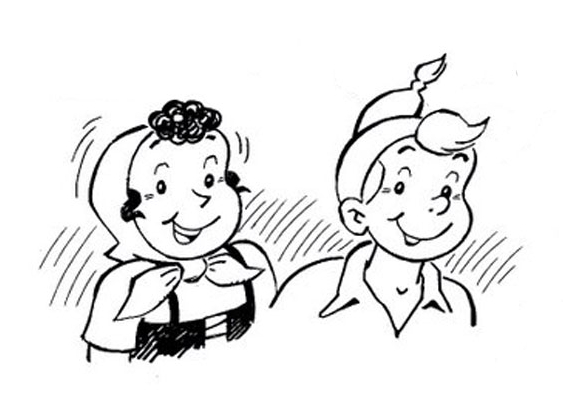
\includegraphics[width=.6\textwidth]{Sylvain+Sylvette_NB.jpg}} 
\newpage

\subsubsection{Exemple \no 7}

Sylvain part à bicyclette de A et se dirige vers B. Il roule à $20$ km/h.



Après avoir parcouru 8 km, il revient en A, s'arrête 12 minutes, puis repart vers B.

Sylvette va directement de A vers B. Elle roule à 16 km/h.

Sylvain et Sylvette sont partis en même temps de A et sont arrivés ensemble à B.

Quelle est la distance entre A et B ? 




\begin{enumerate}
\item \textbf{Choix de l'inconnue}

      Soit d la distance entre A et B. (l'unité est le kilomètre)

\item \textbf{ Mise en équation du problème}

Temps mis par Sylvain : $\dfrac{d+16}{20} + 0,2$

Temps mis par Sylvette : $\dfrac{d}{16}$

$\dfrac{d+16}{20} + \dfrac{1}{5} = \dfrac{d}{16} $


\item \textbf{ Résolution de l'équation}

$\dfrac{d+16}{20} + \dfrac{1}{5} = \dfrac{d}{16} $

$\dfrac{d+16}{20} + \dfrac{4}{20} = \dfrac{d}{16} $

$\dfrac{d+20}{20} = \dfrac{d}{16} $

$\dfrac{4\left(d+20\right)}{80} = \dfrac{5d}{80} $

$4\left(d+20\right) = 5d $

$ 4d + 80 = 5d$

$ -d = -80 $

$ d = 80 $

\item \textbf{ Réponse au problème}

La distance entre A et B est de 80 km.

\end{enumerate}


\newpage

\subsubsection{Exemple \no 8}



Sylvain et Sylvette partent simultanément pour effectuer un trajet de 54 km.


La vitesse de Sylvain est supérieure de 6 km/h à celle de Sylvette.

Sylvain arrive 45 min avant Sylvette.

Quelles sont les vitesses respectives de Sylvain et Sylvette ?



\begin{enumerate}
\item \textbf{Choix de l'inconnue}

Soit V la vitesse de Sylvette en km/h.

\item \textbf{Mise en équation du problème}

Temps mis par Sylvain : $\dfrac{54}{V+6}$

Temps mis par Sylvette : $\dfrac{54}{V}$

$\dfrac{54}{V+6} + \dfrac{3}{4} = \dfrac{54}{V}$

\item \textbf{Résolution de l'équation}

$\dfrac{54}{V+6} + \dfrac{3}{4} = \dfrac{54}{V}$

$\dfrac{216}{4V+24} + \dfrac{3V+18}{4V+24} = \dfrac{54}{V}$

$V\left(216+3V+18\right)=54\left(4V+24\right) $

$ 216V + 3V^2 + 18V = 216V + 1296 $

$ 3V^2 + 18V -1296 = 0 $

$ 3\left(V^2 + 6V - 432\right)=0 $

$ 3\left[\left(V^2 + 6V +9\right) - 441\right] = 0 $

$ 3\left(V+3\right)^2 - 21^2 = 0 $

$ 3\left(V + 3 + 21 \right)\left(V+3-21\right)=0 $

$ 3\left(V+24\right)\left(V-18\right) = 0 $ \\

\begin{tabular}{lcl}
$V+24 = 0$ & ou &$V-18=0$\\
$V=-24$ & ou &$V=18$\\
\end{tabular} \\

Une vitesse ne peut être négative, donc $V=18$.

On sait que la vitesse de Sylvain est $V+6$. Donc la vitesse de Sylvette est de 18 hm/h et celle de Sylvain 24 km/h.
\end{enumerate}



\ifdefined\COMPLETE
\else
    \end{document}
\fi             \newpage  $\;$ \newpage

\section{Inéquations à une inconnue}


\subsection{Inéquations du premier degré}

$ 2x - 5 \leqslant 0 $\\

$2x \leqslant 5 $\\

$ x \leqslant \dfrac{5}{2} $\\ 

Résoudre l'inéquation $ 2x-5\leqslant 0 $, c'est trouver l'ensemble des nombres réels x tels que :\\

$ 2x -5 \leqslant 0 $.

\vspace*{-.3cm}
\begin{tikzpicture}
     \tkzInit[xmin=-30,xmax=20,xstep=6]
     \tkzDrawX[label={},noticks,nograd]
     
     \tkzXHW    % I=]-10,7[
     {
%      -30/T//-10/T/],        % On hachure  de -inf à -10
        7/T/[/20/T/          % et de 9 à +inf
     }
%     \tkzText(-10,-.5){a}    % Etiquette gauche
     \tkzText(6.5,.6){$\dfrac{5}{2}$}      % Etiquette droite
%     \tkzText(0,0){\textcolor{red}{$\times$}}  % Etiquette croix sur R
%     \tkzText(0,-.3){\textcolor{red}{$x$}}     % Etiquette x sous croix
\end{tikzpicture}

$ S = \left]-\infty ; \dfrac{5}{2}\right[ $ \\

Néanmoins, il faut faire attention, car parfois, le sens se modifie : \\

$ -3x + 7 < 0 $\\

$ -3x < -7 $\\

$ 3x > 7 $\\

$ x > \dfrac{7}{3} $ 

\vspace*{-.3cm}
\begin{tikzpicture}
     \tkzInit[xmin=-30,xmax=20,xstep=6]
     \tkzDrawX[label={},noticks,nograd]
     
     \tkzXHW {
      -30/T//-10/T/]        % On hachure  de -inf à -10
%        7/T/[/20/T/          % et de 9 à +inf
     }
     \tkzText(-9.5,.6){$\dfrac{7}{3}$}    % Etiquette gauche
%     \tkzText(6.5,.6){$\dfrac{5}{2}$}      % Etiquette droite
%     \tkzText(0,0){\textcolor{red}{$\times$}}  % Etiquette croix sur R
%     \tkzText(0,-.3){\textcolor{red}{$x$}}     % Etiquette x sous croix
\end{tikzpicture}

\hspace*{4cm}$ S = \left]\dfrac{7}{3}, +\infty\right[ $ \\

\textbf{Attention à certaines inéquations}

$ 2x + 3 \leqslant x + 1 + x + 7 $\\

$ 2x - 2x \leqslant 1 + 7 - 3 $\\

$ 0x \leqslant 5 $ \\

Toujours vrai, donc : $ S = \R = \left]-\infty, +\infty\right[ $ \\

\newpage 

\textbf{Remarque}

Pour les 3 autres équations de la même famille, on aurait : 

$ 0x < 5 $ donne $ S = \R = \left]-\infty, +\infty\right[ $\\

$ 0x > 5 $ donne $ S = \varnothing $\\

$ 0x \geqslant 5 $ donne $ S = \varnothing $ \\

Pour $ 3 + 5x > 2 + 3x + 1 + 2x $, on a :\\

$ -3x - 2x + 5x > 1 + 2 - 3 $\\

$ 0x > 0 $ 

Impossible, donc $ S = \varnothing $ \\

\newpage 
\subsection{Signe de $\mathbf{ax+b}$ (Tableau de signes)}

\begin{tabular}{rl}
Soit : & $ f : \R \rightarrow \R$\\
& $ x\mapsto f(x) = ax + b $ avec $ a \neq 0 $ \\
&\\
& \textbf{Remarque}\\
& La fonction $f$ est une fonction affine, car $ f(x) = ax + b $\\
\end{tabular}

\subsubsection{Exemple \no 1}

Si $ f(x) = 2x-5 $ avec $a = 2$ et $b = -5$, on a : \\

\begin{tabular}{ccc}

$f(x) = 0$ & $f(x) < 0 $ & $f(x) > 0$ \\
\\
$2x - 5 = 0$ & $2x - 5 < 0$ & $2x - 5 > 0$ \\
$2x = 5 $ & $ 2x < 5 $ & $2x > 5 $ \\
$ x = \dfrac{5}{2} $ & $x <\dfrac{5}{2}$ & $x>\dfrac{5}{2}$ \\
\end{tabular}\\


\begin{tikzpicture} 

\tkzTabInit[lgt=2,espcl=1] 
{ $x$         /1, 
$2x-5$   /1}
{$ - \infty $ , $ \dfrac{5}{2} $ , $ + \infty $}
\tkzTabLine{ , - , z , + , }

\end{tikzpicture} 


\subsubsection{Exemple \no 2}

$ f(x) = -3x + 7 $ \\

\begin{tabular}{ccc}

$f(x) = 0$ & $f(x) < 0 $ & $f(x) > 0$ \\

$-3x +7 = 0$ & $-3x +7 < 0$ & $-3x +7 > 0$ \\
$-3x = -7 $ & $ -3x < -7 $ & $-3x > -7 $ \\
$ x = \dfrac{7}{3} $ & $x >\dfrac{7}{3}$ & $x<\dfrac{7}{3}$ \\
\end{tabular}

\begin{tikzpicture} 

\tkzTabInit[lgt=2,espcl=1] 
{ $x$         /1, 
$-3x+7$   /1}
{$ - \infty $ , $ \dfrac{7}{3} $ , $ + \infty $}
\tkzTabLine{ , + , z , - , }

\end{tikzpicture} 

\subsubsection{Tableau récapitulatif}

$ f(x) = ax + b $ avec $ a \neq 0 $ 

$ ax + b = 0 $

$ax = -b $

$ x = -\dfrac{b}{a} $

\vspace {.5cm}

\begin{tikzpicture} 

\tkzTabInit[lgt=4,espcl=3] 
{ $x$ /1, 
$ax+b$  /1}
{$ - \infty $ , $-\dfrac{b}{a} $ , $ + \infty $}
\tkzTabLine{ , $Signe de $-a$$ , z , $Signe de $a$$ }
\end{tikzpicture} 


\subsection{Inéquations produit}

\subsubsection*{Comment faire ?}

\textbf{Exemple \no 0}

$ \left(2x + 5\right)\left(-3x + 7\right) \leqslant 0 $ \\

Il faut faire un tableau de signes : \\

\begin{tikzpicture}

\tkzTabInit[lgt=3,espcl=2]
{ $x$  /1,
$2x+5$   /1,
$-3x + 7$ /1,
$\left(2x+5\right)\left(-3x+7\right)$ /1}
{$ - \infty $ , $-\dfrac{5}{2} $ , $\dfrac{7}{3} $ , $ + \infty $}
\tkzTabLine{ , - , z , +, t  ,+  }
\tkzTabLine{ , + , t , + , z, - }
\tkzTabLine{ , - , z , +, z, - }
\draw[decoration={brace, mirror, raise=0.2cm}, decorate, line width=2pt,black] (T14) -- (N24) ;
\draw[decoration={brace, mirror, raise=0.2cm}, decorate, line width=2pt,black] (N34) -- (T24) ;
\end{tikzpicture}
\\

\begin{tabular}{ccc}
$2x-5=0$& et &$-3x + 7 = 0$ \\
\\
$2x = -5$& et &$-3x = 7 $ \\
\\
$x= -\dfrac{5}{2}$& et & $x=\dfrac{7}{3}$ \\
\end{tabular}\\

\vspace{.1cm}

$ S = \left]-\infty, -\dfrac{5}{2}\right]\cup\left[\dfrac{7}{3},+\infty\right[ $ \\

\textbf{Exemple \no 1}\\

$ x^2 - 9 \leqslant 0 $\\

$ \left(x+3\right)\left(x-3\right) \leqslant 0 $\\

\begin{tabular}{lcl}

$x+3$ & ou & $ x - 3 = 0 $ \\
$x=-3$ & ou & $ x = 3 $ \\
\end{tabular}

\vspace{.5cm}

\begin{tikzpicture}
\tkzTabInit[lgt=3,espcl=2] 
{ $x$        /1 , 
$x+3$ /1 ,
$x-3$ /1,
$\left(x+3\right)\left(x-3\right)$ /1}
{$ -\infty $ , $-3 $ , $3$ , $ +\infty $}
\tkzTabLine{ , - , z , +, t  ,+  }
\tkzTabLine{ , - , t , - , z, + }
\tkzTabLine{ , + , z , -, z, + }
\end{tikzpicture} 

\newpage

\textbf{Exemple \no 2}

$ -x^2+5x < 0 $\\

$ x\left(-x+5\right) = 0$\\

\vspace{.5cm}

\begin{tikzpicture}
\tkzTabInit[lgt=3,espcl=2] 
{ $x$        /1 , 
$x$        /1 , 
$-x+5$ /1 ,
$x\left(-x+5\right)$ /1}
{$ -\infty $ , $0 $ , $5$ , $ +\infty $}
\tkzTabLine{ , - , z , +, t  ,+  }
\tkzTabLine{ , + , t , + , z, - }
\tkzTabLine{ , - , z , +, z, - }
\draw[decoration={brace, mirror, raise=0.2cm}, decorate, line width=2pt,black] (T14) -- (N24) ;
\draw[decoration={brace, mirror, raise=0.2cm}, decorate, line width=2pt,black] (N34) -- (T24) ;
\end{tikzpicture}
\\


$ S = \left]-\infty, 0 \right[\cup\left]5, +\infty\right[ $ \\

\textbf{Exercice \no 1}\\

$ x^2+24x-52 \geqslant 0 $

... 

$ \left(x+26\right)\left(x-2\right) \geqslant 0 $ \\

\begin{tabular}{ccc}
$x+26$ & ou & $x-2 = 0$ \\
$x=-26$ & ou &$x=2$ \\
\end{tabular}

\vspace{.5cm}

\begin{tikzpicture}

\tkzTabInit[lgt=3,espcl=2]
{ $x$  /1,
$x+26$   /1,
$x-2$ /1,
$\left(x+26\right)\left(x-2\right)$ /1}
{$ - \infty $ , $-26 $ , $2 $ , $ + \infty $}
\tkzTabLine{ , - , z , +, t  ,+  }
\tkzTabLine{ , - , t , - , z, + }
\tkzTabLine{ , + , z , -, z, + }
\draw[decoration={brace, mirror, raise=0.2cm}, decorate, line width=2pt,black] (T14) -- (N24) ;
\draw[decoration={brace, mirror, raise=0.2cm}, decorate, line width=2pt,black] (N34) -- (T24) ;
\end{tikzpicture}
\\

$ S = \left]-\infty, -26\right]\cup\left[2, +\infty\right[ $ \\


\newpage 

\textbf{Exercice \no 2}\\

$-9x^2+21x+8 > 0 $

...

$ \left(3x+1\right)\left(3x-8\right)<0 $

\begin{tabular}{ccc}
$3x + 1 = 0$ & ou & $3x - 8 = 0 $ \\
$x = -\dfrac{1}{3} $ & ou & $x=\dfrac{8}{3} $ \\
\end{tabular}\\

\begin{tikzpicture}
\tkzTabInit[lgt=3,espcl=2,]
{ $x$  /1,
$3x+1$   /1,
$3x - 8$ /1,
$\left(3x+1\right)\left(3x-8\right)$ /1}
{$ - \infty $ , $-\dfrac{1}{3} $ , $\dfrac{8}{3} $ , $ + \infty $}
\tkzTabLine{ , - , z , +, t  ,+  }
\tkzTabLine{ , - , t , - , z, + }
\tkzTabLine{ , + , z , -, z, + }
\draw[decoration={brace, mirror, raise=0.2cm}, decorate, line width=2pt,black] (N24) -- (N34) ;

\end{tikzpicture}

$ S = \left]-\dfrac{1}{3}, \dfrac{8}{3} \right[ $ \\

\textbf{Attentions à certaines inéquations}

\textbf{Exemple \no 1}\\

$ 49x^2 - 14x + 1 \leqslant 0 $\\

$ \left(7x-1\right)^2 \leqslant 0 $ \\

$ 7x - 1 = 0 $\\

$ 7x = 1 $\\

$ x = \dfrac{1}{7} $

\begin{tikzpicture}

\tkzTabInit[lgt=3,espcl=2]
{ $x$  /1,
$7x-1$   /1,
$7x-1$ /1,
$\left(7x-1\right)^2$ /1}
{$ - \infty $ , $\dfrac{1}{7} $ , $ + \infty $}
\tkzTabLine{ , - , z , +  }
\tkzTabLine{ , - , z , + }
\tkzTabLine{ , + , z , +, }
\end{tikzpicture}

$ S = \lb \dfrac{1}{7} \rb $ \\

\textbf{Remarque :}

Pour les 3 autres inéquations de la même famille, on aura :

\begin{tabular}{cc}
$49x^2 - 14x + 1 < 0$ & $S = \varnothing$ \\
$49x^2 - 14x + 1 \geqslant 0$& $ S = \R = \left]-\infty ; +\infty\right[$ \\
$49x^2 - 14x + 1 > 0$ & $ S = \left]-\infty ; \dfrac{1}{7} \right[\cup \left]\dfrac{1}{7}; +\infty\right[ $ \\
\end{tabular}

\newpage 

\textbf{Exemple \no 2} 

$ 25x^2 + 20x + 13 \leqslant 0 $\\

$ 25x^2 + 20x + 4 + 9 \leqslant 0 $\\

$ \left(5x + 2\right)^2 + 9 \leqslant 0 $\\

$ \left(5x + 2\right)^2 \leqslant - 9 $\\

Or, le carré d'un nombre est toujours positif. \\
Donc $ S = \varnothing $.\\

\textbf{Remarque :}

Pour les 3 autres inéquations de la même famille, on aura :

\begin{tabular}{cc}
$25x^2 + 20x + 13 < 0$ & $S = \varnothing$ \\
$25x^2 + 20x + 13 < 0$ & $ S = \R = \left]-\infty ; +\infty\right[$ \\
$25x^2 + 20x + 13 < 0$ & $ S = \R = \left]-\infty ; +\infty\right[$ \\
\end{tabular}

\newpage 
\subsection{Inéquation avec l'inconnue au dénominateur}

$ \dfrac{6}{x-2} \leqslant x-3 $\\

\textbf{Il ne faut pas que $ x-2 = 0 $ donc que $ x = 2 $}\\

\textbf{Valeur interdite : $ x = 2 $}\\

\textbf{Attention, dans le cas des inéquations, le produit en croix est interdit}\\

$ \dfrac{6}{x-2} - \left(x-3\right) \leqslant 0 $\\

$ \dfrac{6 - \left(x-2\right)\left(x-3\right)}{x-2} \leqslant 0 $\\

$ \dfrac{6 - \left(x^2 - 5x + 6 \right)}{x-2} \leqslant 0 $\\

$ \dfrac{-x^2 + 5x}{x-2} \leqslant 0 $\\

\vspace{.5cm}

\begin{tikzpicture}

\tkzTabInit[lgt=3,espcl=2,]
{ $x$  /1,
$x$ /1,
$-x+5$   /1,
$x -2 $ /1,
$\dfrac{x\left(-x+5\right)}{x-2}$ /1}
{$ - \infty $ , $0 $ , $2 $ , $5$ , $ + \infty $}
\tkzTabLine{ , - , z , +, t  ,+ , t , + }
\tkzTabLine{ , + , t , + , t , + , z, - }
\tkzTabLine{ , - , t , - , z , + , t , + }
\tkzTabLine{ , + , z , - , d , + , z , - }
\draw[decoration={brace, mirror, raise=0.2cm}, decorate, line width=2pt,black] (N25) -- (N35) ;
\draw[decoration={brace, mirror, raise=0.2cm}, decorate, line width=2pt,black] (N45) -- (T25) ;
\end{tikzpicture}
\\

$ S = \left[0,2\right[\cup \left[5, + \infty \right[ $ \\
\newpage
\textbf{Exercice \no 2} \\

$ \dfrac{x^2-15}{\left(x-4\right)\left(x-3\right)} \geqslant \dfrac{1}{x-4} - \dfrac{1}{x-3} $ \\

\textbf{Valeurs interdites : $x=4 $ et $ x = 3 $}  \\

$ \dfrac{x^2-15}{\left(x-4\right)\left(x-3\right)} \geqslant \dfrac{\left(x-3\right)-\left(x-4\right)}{\left(x-4\right)\left(x+3\right)} $ \\

$ \dfrac{x^2-15}{\left(x-4\right)\left(x-3\right)} \geqslant \dfrac{1}{\left(x-4\right)\left(x+3\right)} $ \\

$ \dfrac{x^2-15-1}{\left(x-4\right)\left(x-3\right)} \geqslant 0  $ \\

$ \dfrac{x^2-16}{\left(x-4\right)\left(x-3\right)} \geqslant 0  $ \\

$ \dfrac{\left(x+4\right)\left(x-4\right)}{\left(x-4\right)\left(x-3\right)} \geqslant 0  $ \\

\textbf{Remarque}

Simplifier est alors dangereux... Il est plus prudent d'écrire le tableau de signes ainsi : \\

\begin{tikzpicture}

\tkzTabInit[lgt=3,espcl=2]
{ $x$  /1,
$x+4$ /1,
$x-4$   /1,
$x-4 $ /1,
$x-3$ /1,
$\dfrac{x\left(x+4\right)\left(x-4\right)}{\left(x-4\right)\left(x-3\right)}$ /1}
{$ - \infty $ , $-4 $ , $3 $ , $4$ , $ + \infty $}
\tkzTabLine{ , - , z , +, t  ,+ , t , + }
\tkzTabLine{ , - , t , - , t , - , z, + }
\tkzTabLine{ , - , t , - , t , - , z, + }
\tkzTabLine{ , - , t , - , z , + , t , + }
\tkzTabLine{ , + , z , - , d , + , d , + }
\draw[decoration={brace, mirror, raise=0.2cm}, decorate, line width=2pt,black] (T16) -- (N26) ;
\draw[decoration={brace, mirror, raise=0.2cm}, decorate, line width=2pt,black] (N36) -- (N46) ;
\draw[decoration={brace, mirror, raise=0.2cm}, decorate, line width=2pt,black] (N46) -- (T26) ;
\end{tikzpicture}\\

$S=\left]-\infty,-4\right]\cup\left]3,4\right[\cup\left]4,+\infty\right[$

\newpage 
\subsection{Systèmes d'inéquations}

\subsubsection{Exemple \no 1}

\vspace*{.5cm}

\begin{minipage}{3cm}
\begin{equation*}
\left\lbrace \begin{aligned}
2x+3      &> 3x-2\\
3(x-2)    &\geqslant 2-5x\\
\end{aligned}
\right.
\end{equation*}
\end{minipage}

\vspace*{.5cm}

Résoudre un tel système, c'est trouver l'ensemble des nombres réels $x$ \\
tels que $ 2x + 3 > 3x - 2 $ 
\textbf{et} $ 3\left(x-2\right) \geqslant 2 -5x $\\

\textbf{1$^{re}$ inéquation :}\\

$2x + 3 > 3x - 2$\\

$- x > -5$\\

$x < 5$ \\

$ S_1 = \left]-\infty, 5 \right[ $ \\

\textbf{2$^{me}$ inéquation :}\\

$ 3\left(x-2\right) \geqslant 2 - 5x $\\

$ 3x - 5 \geqslant 2 - 5x $\\

$ 8 x \geqslant 8 $\\

$ x \geqslant 1 $ \\

$ S_2 = \left[1, +\infty\right[ $ \\

\textbf{3 : Système}\\

$ S = S_1 \cap S_2 $


\vspace*{-.3cm}
\begin{tikzpicture}
     \tkzInit[xmin=-30,xmax=20,xstep=6]
     \tkzDrawX[label={},noticks,nograd]
     
      \tkzDefPoint(-30,-.05){A1} 
      \tkzDefPoint(7,-.05){A2} 
     \tkzDrawSegment[color=green](A1,A2) ; 
       \tkzXHW [color=green]  % XHW : hachures SW -> NE  
     {
%      -30/T//-10/T/],        % On hachure  de -inf à -10
        7/T/[/20/T/          % et de 9 à +inf
     }
        
     \tkzDefPoint(-10,.05){B1} 
      \tkzDefPoint(20,.05){B2} 
     \tkzDrawSegment[color=red](B1,B2) ; 
     \tkzXH [color=red]   % XH : hachures NW -> SE
     {
      -30/T//-10/T/[        % On hachure  de -inf à -10
%        7/T/[/20/T/          % et de 9 à +inf
     }
     
     \tkzText(-10,.5){$1$}    % Etiquette gauche
     \tkzText(6.5,.6){$5$}      % Etiquette droite
%     \tkzText(0,0){\textcolor{red}{$\times$}}  % Etiquette croix sur R
%     \tkzText(0,-.3){\textcolor{red}{$x$}}     % Etiquette x sous croix
\end{tikzpicture}


$ S= \left[1,5\right[ $
\newpage
\subsubsection{Exemple \no 2}

\vspace*{.5cm}

\begin{minipage}{3cm}
\begin{equation*}
\left\lbrace \begin{aligned}
\dfrac{3}{5}x     &  >     \dfrac{1}{5} + x \\
6\left(2-x\right) & \leqslant   -2x \\
\end{aligned}
\right.
\end{equation*}
\end{minipage}

\vspace*{.5cm}

\textbf{1$^{re}$ inéquation :}

$ \dfrac{3}{5}x - x > \dfrac{1}{5} $\\

$ x \left(\dfrac{3}{5} - 1\right) > \dfrac{1}{5} $\\

$ -\dfrac{2}{5}x > \dfrac{1}{5} $\\

$ x < \dfrac{1}{5} \times \left(-\dfrac{5}{2}\right) $\\

$ x < -\dfrac{1}{2} $ \\

$ S_1 = \left]-\infty, -\dfrac{1}{2} \right[ $\\

\textbf{2$^{me}$ inéquation :}

$12 - 6x \leqslant -2x $\\

$ -4x \leqslant -12 $\\

$ 4x \geqslant 12 $\\

$ x \geqslant 3 $ \\

$ S_2 = \left[3, +\infty\right[ $\\

\textbf{3 : Système}\\

$ S = S_1 \cap S_2 = \varnothing $\\

\vspace*{-.3cm}
\begin{tikzpicture}   
     \tkzInit[xmin=-5,xmax=7]
     \tkzDrawX[label={},noticks,nograd]
     
      \tkzDefPoint(3,.1){A1} 
      \tkzDefPoint(7,.1){A2} 
     \tkzDrawSegment[color=red](A1,A2) ; 
       \tkzXH [color=red]  % XHW : hachures SW -> NE  
     {
        -5/T//3/T/[          % True de 3 à +inf 
     }
        
     \tkzDefPoint(-5,-.1){B1} 
      \tkzDefPoint(-1/2,-.1){B2} 
     \tkzDrawSegment[color=blue](B1,B2) ; 
     \tkzXHW [color=blue]   % XH : hachures NW -> SE
     {
      -.5/T/[/7/T/        % On hachure  de -inf à -10
     }
     
    \tkzText(-1/2,.5){$-\dfrac{1}{2}$}    % Etiquette gauche
    \tkzText(3,.6){$3$}      % Etiquette droite
\end{tikzpicture}

\textbf{Remarque}

Les 2 inéquations sont incompatibles.
\newpage 
\subsubsection{Exercice \no 1}

\begin{minipage}{3cm}
\begin{equation*}
\left\lbrace \begin{aligned}
4x^2 + 3x + 1&\geqslant x^2 - 3x + 1\\
\left(x+1\right)^2&> 5x+5 \\
\end{aligned}
\right.
\end{equation*}
\end{minipage}

\vspace{.5cm}

\textbf{1$^{re}$ inéquation}\\

$ 3x^2 + 6x \geqslant 0 $

$ 3x \left(x+2\right) \geqslant 0 $\\ 

\begin{tikzpicture}
\tkzTabInit[lgt=3,espcl=2]
{ $x$  /1,
$3x$ /1,
$x+2$   /1,
$3x\left(x+2\right)$ /1}
{$ - \infty $ , $-2 $ , $0 $ , $ + \infty $}
\tkzTabLine{ , - , t , -, z  ,+ }
\tkzTabLine{ , - , z , + , t , + }
\tkzTabLine{ , + , z , - , z , + }
\draw[decoration={brace, mirror, raise=0.2cm}, decorate, line width=2pt,black] (T14) -- (N24) ;
\draw[decoration={brace, mirror, raise=0.2cm}, decorate, line width=2pt,black] (N34) -- (T24) ;
\end{tikzpicture}


$ S_1 = \left]-\infty, -2\right]\cup[0,+\infty[ $ \\

\textbf{2$^{me}$ inéquation}\\

$ \left(x+1\right)^2 > 5\left(x+1\right) $

$ \left(x+1\right)^2 - 5\left(x+1\right)  > 0 $

$ \left(x+1\right)\left(x+1-5\right) > 0 $

$ \left(x+1\right)\left(x-4\right) > 0 $\\



\begin{tikzpicture}
\tkzTabInit[lgt=3,espcl=2]
{ $x$  /1,
$x+1$ /1,
$x-4$   /1,
$\left(x+1\right)\left(x-4\right)$ /1}
{$ - \infty $ , $-1 $ , $4 $ , $ + \infty $}
\tkzTabLine{ , - , z , +, t  ,+ }
\tkzTabLine{ , - , t , - , z , + }
\tkzTabLine{ , + , z , - , z , + }
\draw[decoration={brace, mirror, raise=0.2cm}, decorate, line width=2pt,black] (T14) -- (N24) ;
\draw[decoration={brace, mirror, raise=0.2cm}, decorate, line width=2pt,black] (N34) -- (T24) ;
\end{tikzpicture}\\

$ S_2 = \left]-\infty, -1\right[\cup\left]4, + \infty \right[ $\\

\textbf{3 : Système}

$ S = S_1 \cap S_2 = \left]-\infty, -2\right]\cup\left]4, + \infty\right[ $\\


\begin{tikzpicture}   
     \tkzInit[xmin=-5,xmax=7]
     \tkzDrawX[label={},noticks,nograd]
     
      \tkzDefPoint(-5,.1){A1} 
      \tkzDefPoint(-1,.1){A2} 
      \tkzDefPoint(4,.1){A3} 
      \tkzDefPoint(7,.1){A4} 
      \tkzDrawSegments[color=red](A1,A2 A3,A4) ; 
       \tkzXHW [color=red]   
     {
        -1/T/[/4/T/]          
     }
        
     \tkzDefPoint(-5,-.1){B1} 
     \tkzDefPoint(-2,-.1){B2}
     \tkzDefPoint(0,-.1){B3} 
     \tkzDefPoint(7,-.1){B4}  
     \tkzDrawSegments[color=blue](B1,B2 B3,B4) ; 
     \tkzXH [color=blue]  
     {
      -2/T/]/0/T/[       
     }
     
    \tkzText(-2,.5){$-2$} 
    \tkzText(-1,.5){$-1$}  
    \tkzText(0,.5){$0$}   
    \tkzText(4,.5){$4$}  
\end{tikzpicture}

\newpage 

\subsubsection{Exercice \no 2}

$ 0 \leqslant \left(3x-8\right)^2-\left(x-4\right)^2 \leqslant 48 $

C'est une \textbf{double inéquation}, cela veut dire que : \\

$ \left(3x-8\right)^2-\left(x-4\right)^2 \geqslant 0 $

$ \left(3x-8\right)^2-\left(x-4\right)^2 \leqslant 48 $ \\

\textbf{1$^{re}$ inéquation}

$ \left(3x-8+x+4\right)\left[\left(3x-8\right)-\left(x+4\right)\right] \geqslant 0 $

$ \left(3x-8+x+4\right)\left(3x-8-x-4\right) \geqslant 0 $

$ \left(4x-4\right)\left(2x-12\right) \geqslant 0 $ \\

\begin{tikzpicture}
\tkzTabInit[lgt=3,espcl=2]
{ $x$  /1,
$4x-4$ /1,
$2x-12$   /1,
$\left(4x-4\right)\left(2x-12\right)$ /1}
{$ - \infty $ , $1 $ , $6 $ , $ + \infty $}
\tkzTabLine{ , - , z , +, t  ,+ }
\tkzTabLine{ , - , t , - , z , + }
\tkzTabLine{ , + , z , - , z , + }
\draw[decoration={brace, mirror, raise=0.2cm}, decorate, line width=2pt,black] (T14) -- (N24) ;
\draw[decoration={brace, mirror, raise=0.2cm}, decorate, line width=2pt,black] (N34) -- (T24) ;
\end{tikzpicture}

$ S_1 = \left]-\infty, 1 \right]\cup\left[6, + \infty\right[ $ \\

\textbf{2$^{me}$ inéquation}

$ \left(3x-8\right)^2-\left(x+4\right)^2 \leqslant 48 $

$ \left(9x^2 - 48x + 64\right)-\left(x^2+8x+16\right) \leqslant 48 $

$ 9x^2 - 48x + 64 -x^2- 8x- 16 \leqslant 48 $

$ 8x^2 -56x + 48 \leqslant 48 $

$ 8x^2 - 56x \leqslant 0 $

$ 8x \left(x-7\right)\leqslant 0 $\\

\begin{tikzpicture}
\tkzTabInit[lgt=3,espcl=2]
{ $x$  /1,
$8x$ /1,
$x-7$   /1,
$8x\left(x-7\right)$ /1}
{$ - \infty $ , $0 $ , $7 $ , $ + \infty $}
\tkzTabLine{ , - , z , +, t  ,+ }
\tkzTabLine{ , - , t , - , z , + }
\tkzTabLine{ , + , z , - , z , + }
\draw[decoration={brace, mirror, raise=0.2cm}, decorate, line width=2pt,black] (N24) -- (N34) ;
\end{tikzpicture}

$ S_2 = \left[0,7\right] $ \\

\textbf{3 : Système}\\

$ S = S_1 \cap S_2 = \left[0,1\right]\cup \left[6,7\right] $\\

\begin{tikzpicture}   
     \tkzInit[xmin=-2,xmax=9]
     \tkzDrawX[label={},noticks,nograd]
 
       \tkzXHW [color=blue]   
     {
        -2/T//0/T/[,   
         7/T/]/9/T/           
     }

     \tkzXH [color=blue]  
     {
      1/T/]/6/T/[       
     }
     
    \tkzText(0,.5){$0$} 
    \tkzText(1,.5){$1$}  
    \tkzText(6,.5){$6$}   
    \tkzText(7,.5){$7$}  
\end{tikzpicture}
\subsubsection{Exercice \no 3}

$ 2 \leqslant \dfrac{x+5}{x+2} \leqslant 3 $ \\

\textbf{Valeur interdite : $\mathbf{x = -2 }$} \\

Pour la première inéquation, on a :\\

$ \dfrac{-x+1}{x+2} \geqslant 0 $ \\

\vspace{.5cm}

\begin{tikzpicture}
\tkzTabInit[lgt=3,espcl=2]
{ $x$  /1,
$-x+1$ /1,
$x+2$   /1,
$\left(-x+1\right)\left(x+2\right)$ /1}
{$ - \infty $ , $-2 $ , $1 $ , $ + \infty $}
\tkzTabLine{ , + , t , +, z  ,- }
\tkzTabLine{ , - , z , + , t , + }
\tkzTabLine{ , - , d , + , z , - }
\draw[decoration={brace, mirror, raise=0.2cm}, decorate, line width=2pt,black] (N24) -- (N34) ;
\end{tikzpicture}
\\

$ S_1 = \left]-2, 1 \right] $ \\

Pour la deuxième inéquation, on a : \\

$ \dfrac{-2x-1}{x+2} \leqslant 0 $ \\

\vspace{.5cm}

\begin{tikzpicture}
\tkzTabInit[lgt=3,espcl=2]
{ $x$  /1,
$-2x-1$ /1,
$x+2$   /1,
$\left(-2x-1\right)\left(x+2\right)$ /1}
{$ - \infty $ , $-2 $ , $-\dfrac{1}{2} $ , $ + \infty $}
\tkzTabLine{ , +, t , +, z  ,- }
\tkzTabLine{ , - , z , + , t , + }
\tkzTabLine{ , - , d , + , z , - }
\draw[decoration={brace, mirror, raise=0.2cm}, decorate, line width=2pt,black] (T14) -- (N24) ;
\draw[decoration={brace, mirror, raise=0.2cm}, decorate, line width=2pt,black] (N34) -- (T24) ;
\end{tikzpicture}
\\

$ S_2 = \left]-\infty,-2\right[\cup\left[-\dfrac{1}{2}, +\infty \right[ $ \\

$  S = S_1 \cap S_2 = \left[-\dfrac{1}{2}, 1 \right] $\\

\begin{tikzpicture}   
     \tkzInit[xmin=-4,xmax=3]
     \tkzDrawX[label={},noticks,nograd]
 
       \tkzXHW [color=blue]   
     {
        -4/T//-2/T/],   
         1/T/]/3/T/           
     }

     \tkzXH [color=blue]  
     {
      -2/T/]/-.5/T/[       
     }
     
    \tkzText(-2,.5){$-2$} 
    \tkzText(-1/2,.5){$-\dfrac{1}{2}$}  
    \tkzText(1,.5){$1$}   
\end{tikzpicture}

\newpage

\subsection{Exemples de problèmes pratiques}

\subsubsection{Exemple \no 1}

Un motard poursuit une voiture sur l'autoroute. La voiture est à $150$ km de la sortie. Elle roule à 120 km/h. \\ 

Le motard est à $x$ km derrière la voiture. Il roule à $130$ km/h. \\ 

Pour quelles valeurs de $x$ Sylvain rattrape-t-il Sylvette, avant la sortie de l'autoroute ? \\

\textbf{1) Choix de l'inconnue.}

Soit $x$ la distance, en km, qui sépare le motard de la voiture. \\

\textbf{2) Mise en équation du problème} \\

Temps mis par le motard  : $\dfrac{x+150}{130} $ \\

Temps mis par la voiture : $\dfrac{150}{120} $ \\

Donc $ \dfrac{x+150}{130} \leqslant \dfrac{150}{120}$ \\

\textbf{3) Résolution de l'équation}

$ \dfrac{x+150}{130} \leqslant \dfrac{150}{120}$ \\

$ \dfrac{x+150}{130} \leqslant \dfrac{5}{4}$ \\

$ \dfrac{2\left(x+150\right)}{260} \leqslant \dfrac{325}{260} $ \\

$ 2x + 300 \leqslant 325 $ \\

$ 2x \leqslant 25 $ \\

$ x \leqslant 12,5 $ \\

\textbf{4) Réponse au problème}

Donc le motard rattrapera la voiture si la distance qui le sépare est inférieur à $12,5$ km. \\

\newpage

\subsubsection{Exemple \no 2}

Voici les tarifs pratiqués par 3 agences de location de voiture pour des véhicules identiques : \\

\begin{itemize}
\item Agence A : $52,74$\euro par jour et $0,41$ \euro par km ; 
\item Agence B : $43,14$\euro  par jour et $0,49$ \euro par km ; 
\item Agence C : $47,40$\euro par jour et $0,44$ \euro par km. \\
\end{itemize} 

Sylvain et Sylvette désirent parcourir $x$ km par jour. Quelle agence choisissent-ils ? \\

\begin{enumerate}


\item \textbf{Choix de l'inconnue.}

Soit $x$ le nombre de km parcourus. \\

\item \textbf{ Mise en équation du problème} \\

$P_A(x) = 52,74$\euro $+0,41x$ 

$P_B(x) = 43,14$\euro $+0,49x$ 

$P_C(x) = 57,40$\euro $+0,44x$ \\

Sylvain et Sylvette choisissent l'agence A si $P_A(x) \leqslant P_B(x)$ et $ P_A(x) \leqslant P_C(x)$. 

Sylvain et Sylvette choisissent l'agence B si $P_B(x) \leqslant P_A(x)$ et $ P_B(x) \leqslant P_C(x)$. 

Sylvain et Sylvette choisissent l'agence C si $P_C(x) \leqslant P_A(x)$ et $ P_C(x) \leqslant P_B(x)$. \\

\item \textbf{Résolution de l'équation} \\

\begin{enumerate}


\item {$\begin{cases}
52,74+0,41x &\leqslant 43,14+0,49x\\
52,74+0,41x & \leqslant 57,40+0,44x\\
\end{cases}$}

\begin{enumerate}


\item $52,74+0,41x \leqslant 43,14+0,49x$ 

$ -0,08x \leqslant -9,6 $

$ 0,08 \geqslant 9,6 $

$ x \geqslant 120 $ \\

\item $52,74+0,41x \leqslant 57,40+0,44x$

$-0,03x \leqslant -5,34$ 

$ 0,03x \geqslant  5,34 $

$ x \geqslant 178 $ \\


\begin{tikzpicture}   
     \tkzInit[xmin=8,xmax=20]
     \tkzDrawX[label={},noticks,nograd]
 
       \tkzXH [color=blue]   
     {
        8/T//17.8/T/|            
     }

     \tkzXHW [color=blue]  
     {
      8/T//12/T/|       
     }
     
    \tkzText(12,1){$120$} 
    \tkzText(17.8,1){$178$}     
\end{tikzpicture}

Sylvain et Sylvette choisissent l'agence A s'ils parcourent une distance supérieure à $178$ km. \\
\end{enumerate}
\newpage

\item  $\begin{cases}
43,14+0,49x &\leqslant 52,74+0,41x\\
43,14+0,49x & \leqslant 57,40+0,44x\\
\end{cases}$  \\

\begin{enumerate}
\item $43,14+0,49x \leqslant 52,74+0,41x$ \\

       D'après (a)i. , on a : $x\leqslant 120$ \\

\item $43,14+0,49x \leqslant 57,40+0,44x$\\

$0,05x \leqslant 4,26 $\\

$x \leqslant 85,2 $ \\


\begin{tikzpicture}   
     \tkzInit[xmin=8,xmax=20]
     \tkzDrawX[label={},noticks,nograd]
 
       \tkzXH [color=blue]   
     {
        12/T/|/20/T/            
     }

     \tkzXHW [color=blue]  
     {
      8.52/T/|/20/T/       
     }

    \tkzText(8.52,1){$85,2$}       
    \tkzText(12,1){$120$} 
   
\end{tikzpicture}


Sylvain et Sylvette choisissent l'agence $B$ s'ils parcourent une distance inférieure à $85,2$ km. 
\end{enumerate}

\item  $\begin{cases}
57,40+0,44x &\leqslant 52,74+0,41x\\
57,40+0,44x & \leqslant 43,14+0,49x\\
\end{cases}$  \\

\begin{enumerate}


\item  D'après (a)ii, on a : $x 178$ \\

\item 
 D'après (b)ii, on a : $x\geq 85,2$ \\

\end{enumerate}
\end{enumerate}
\end{enumerate}

\begin{tikzpicture}   
     \tkzInit[xmin=5,xmax=20]
     \tkzDrawX[label={},noticks,nograd]
 
       \tkzXHW [color=blue]   
     {
        17.8/T/|/20/T/            
     }

     \tkzXH [color=blue]  
     {
      5/T//8.52/T/|       
     }

    \tkzText(8.52,1){$85,2$}       
    \tkzText(17.8,1){$178$} 
   
\end{tikzpicture}

Sylvain et Sylvette choisissent l'agence $C$ s'ils parcourent une distance comprise entre $85,2$ km et $178$ km. \\


           \newpage  $\;$ \newpage
\ifdefined\COMPLETE
\else
    \input{./preambule-sacha-utf8.ltx}
    \begin{document}
\fi

\section{Fonctions numérique de la variable réelle : Généralités et définitions}

\subsection{Fonction}

\begin{tabular}{lll}
Soit & $f:$ & $ \R \rightarrow \R$ \\
& & $x\mapsto \underbrace{f(x)}_{\textrm{image de} x}$ \\
\end{tabular}

$f$ est une fonction numérique de la variable réelle si et seulement si :

\textbf{Tout élément de $\mathbf{\R}$ a au plus une image dans $\mathbf{\R}$.} \\

\textbf{Remarques}

\begin{itemize}


\item[*]Vocabulaire : "Au plus une" veut dire, soit une, soit aucune. \\ 

\item[*] $f$ est une fonction et $f(x)$ un nombre réel.
\end{itemize}
\subsection{Ensemble de définition d'une fonction}

\begin{tabular}{lll}

Soit & $f:$& $ \R \rightarrow \R$ \\
& & $x\mapsto f(x)$ \\
\end{tabular}

\textbf{L'ensemble de définition de f, noté $ \mathbf{D_f} $, est l'ensemble de élément de $\mathbf{\R}$\\qui ont une image dans $\mathbf{\R}$}


\begin{minipage}{5cm}
\begin{tikzpicture}[scale=.8]

\tkzDefPoint [label=left:$a$](0,1.5){a}
\tkzDrawPoint[size=10,color=black](a)
\tkzDefPoint [label=left:$b$](0,1){b}
\tkzDrawPoint[size=10,color=black](b)
\tkzDefPoint [label=left:$c$](0,.5){c}
\tkzDrawPoint[size=10,color=black](c)
\tkzDefPoint [label=left:$d$](0,0){d}
\tkzDrawPoint[size=10,color=black](d)
\tkzDefPoint [label=right:$\Delta$](3,1.5){de}
\tkzDrawPoint[size=10,color=black](de)
\tkzDefPoint [label=right:$\bigstar$](3,1){st}
\tkzDrawPoint[size=10,color=black](st)
\tkzDefPoint [label=right:$\bigcirc$](3,.5){nada}
\tkzDrawPoint[size=10,color=black](nada)



\node [draw,ellipse,minimum height=3cm,minimum width=1.5cm, fit={(a) (b) (c) (d) }] {};
\node [draw,ellipse,minimum height=3cm,minimum width=1cm,fit={(de) (st) (nada) }] {};

\draw  [bend left=20,-latex](a) to (de) ; 
\draw  [bend right=20,-latex](b) to (de) ; 
\draw  [bend right=20,-latex](c) to (st) ; 
\end{tikzpicture}
\end{minipage}
\begin{minipage}{3cm}

$f(a) = \Delta$

$f(b) = \Delta$

$f(c) = \bigstar $ \\

$ D_f = \lb a, b, c \rb $

$D_f = E \setminus\lb d \rb $

\end{minipage}\\


\subsubsection{Exercice \no 1}

\begin{tabular}{llll}
Soit & $f:$& $ \R \rightarrow \R$ & \\
& & $x\mapsto f(x)$ & $=\dfrac{x-4}{x-2}$ \\
\end{tabular}\\

Il ne faut pas que $x-2=0$, donc que $x=2$.

$D_f = \R \setminus \lb 2 \rb = \left]-\infty,2\right[\cup\left]2, +\infty\right[$

\subsubsection{Exercice \no 2}

\begin{tabular}{llll}

Soit & $f:$& $ \R \rightarrow \R$ & \\
& & $x\mapsto f(x)$ & $=\sqrt{x-2}$ \\
\end{tabular}\\

Il faut que $x-2 \geqslant 0$, donc que $x \geqslant 2 $

$D_f = \left[2, +\infty\right[ $

\newpage

\subsubsection{Exercice \no 3}

\begin{tabular}{llll}

Soit & $f:$& $ \R \rightarrow \R$ & \\
& & $x\mapsto f(x)$ & $=\dfrac{x^2 + 4}{x^2 - 4}$ \\
\end{tabular}\\

Il ne faut pas que $x^2 - 4 = 0$, donc que $\left(x+2\right)\left(x-2\right) = 0 $

\begin{tabular}{lll}
$x+2=0$ & ou & $x-2 = 0 $ \\
$x = -2 $ & ou & $x=2$ \\
\end{tabular}

$ D_f = \R \setminus\lb -2,2\rb = \left]-\infty, -2\right[\cup \left]-2,2\right[\cup\left]2, +\infty\right[ $

\subsubsection{Exercice \no 4}

\begin{tabular}{llll}

Soit & $f:$& $ \R \rightarrow \R$ & \\
& & $x\mapsto f(x)$ & $=\sqrt{x^2 - 4}$ \\
\end{tabular}

Il faut que $x^2 - 4 \geqslant 0 $, donc que $\left(x+2\right)\left(x-2\right) \geqslant 0$

\begin{tikzpicture}
\tkzTabInit[lgt=3,espcl=2]
{ $x$  /1,
$x+2$ /1,
$x-2$   /1,
$\left(x+2\right)\left(x-2\right)$ /1}
{$ - \infty $ , $-2 $ , $2 $ , $ + \infty $}
\tkzTabLine{ , - , z , +, t  ,+ }
\tkzTabLine{ , - , t , - , z , + }
\tkzTabLine{ , + , z , - , z , + }
\draw[decoration={brace, mirror, raise=0.2cm}, decorate, line width=2pt,black] (T14) -- (N24) ;
\draw[decoration={brace, mirror, raise=0.2cm}, decorate, line width=2pt,black] (N34) -- (T24) ;
\end{tikzpicture}

$D_f = \left]-\infty,-2\right[\cup\left[2,+\infty\right[ $

\subsubsection{Exercice \no 5}

\begin{tabular}{llll}

Soit & $f:$& $ \R \rightarrow \R$ & \\
& & $x\mapsto f(x)$ & $=\dfrac{x^2 - 4}{x^2 + 4}$ \\
\end{tabular}\\

Il ne faut pas que $x^2 + 4 = 0$, donc $x^2 = -4$.

Ceci est impossible, donc $D_f = \R$.

\textbf{Remarque}

Il s'agit du problème de la continuité.

\subsubsection{Exercice \no 6}

\begin{tabular}{llll}

Soit & $f:$& $ \R \rightarrow \R$ & \\
& & $x\mapsto f(x)$ & $=\sqrt{x^2 + 4}$ \\
\end{tabular}

Il faut que $x^2+4 \geqslant 0$, donc $x^2 \geqslant -4$

Ceci est toujours vrai, donc $D_f = \R$.

\subsection{Représentation graphique d'une fonction}

\begin{tabular}{lll}

Soit & $f:$& $ \R \rightarrow \R$ \\
& & $x\mapsto f(x)$ \\
\end{tabular}\\

Soit $\left(0, \overrightarrow{i}, \overrightarrow{j}\right)$ un repère.

La représentation graphique de $f$, notée $C_f$, est l'ensemble des points $M\left(x,y\right)$ avec $x\in D_f$ et $y = f(x)$.

\newpage

\vspace*{-2cm}
\textbf{I}\\

\centerline{
\begin{minipage}{.45\textwidth}
\shorthandoff{:}
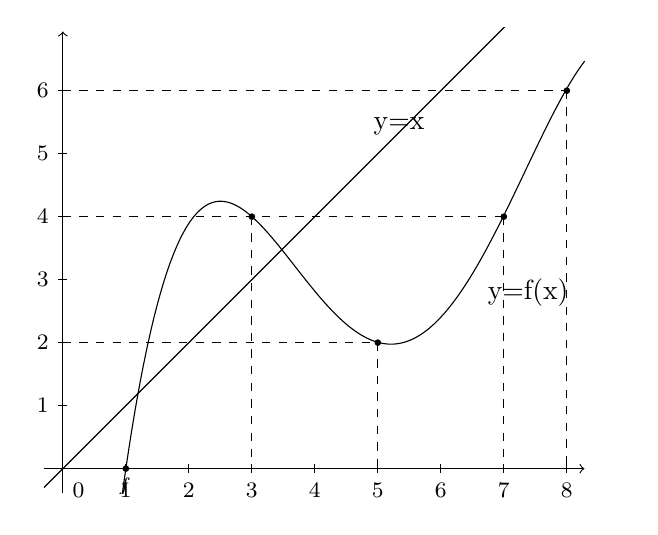
\begin{tikzpicture}[scale=0.8]
\draw[->,color=black] (-0.3,0) -- (8.28,0);
\foreach \x in {,1,2,3,4,5,6,7,8}
\draw[shift={(\x,0)},color=black] (0pt,2pt) -- (0pt,-2pt) node[below] {\footnotesize $\x$};
\draw[->,color=black] (0,-0.38) -- (0,6.94);
\foreach \y in {,1,2,3,4,5,6}
\draw[shift={(0,\y)},color=black] (2pt,0pt) -- (-2pt,0pt) node[left] {\footnotesize $\y$};
\draw[color=black] (0pt,-10pt) node[right] {\footnotesize $0$};
\clip(-0.3,-0.4) rectangle (9,7);
\draw[smooth,samples=100,domain=-0.301:8.284] plot(\x,{
-(29/840)*(\x)^4 
+(213/280)*(\x)^3 
-(4699/840)*(\x)^2 
+(4443/280)*\x 
-11});
\draw [dashed] (3,4)-- (3,0);
\draw [dashed] (0,4)-- (7,4);
\draw [dashed] (7,4)-- (7,0);
\draw [dashed] (0,2)-- (5,2);
\draw [dashed] (5,2)-- (5,0);
\draw [dashed] (0,6)-- (8,6);
\draw [dashed] (8,6)-- (8,0);
\draw[smooth,samples=100,domain=-0.301:8.284] plot(\x,{(\x)});
\draw (6.59,3.17) node[anchor=north west] {y=f(x)};
\draw (4.78,5.72) node[anchor=north west] {y=x};
\begin{scriptsize}
\fill (1,0) circle (1.5pt);
\fill (3,4) circle (1.5pt);
\fill (5,2) circle (1.5pt);
\fill (7,4) circle (1.5pt);
\draw(0.98,-0.29) node {$f$};
\fill (8,6) circle (1.5pt);
\end{scriptsize}
\end{tikzpicture}
\shorthandon{:}
\end{minipage} \hspace*{1cm}
\begin{minipage}{.45\textwidth}
On a représenté ci-contre : \\
\begin{itemize}
\item[*] La droite d'équation $y=x$ ; 
\item[*] La courbe représentative d'une fonction $f$ définie sur l'intervalle $[1;8]$. 
\end{itemize}
Les question posées seront résolues par {\bf lecture graphique}. 
\end{minipage}}
\vspace{.5cm}
Répondre par vrai ou faux aux questions suivantes : 

\vspace{.1cm}

\begin{tabular}{|l|c|l}
\multicolumn{2}{r}{vrai ou faux} & \\
\cline{1-2}
$1$ a pour image $0$ par la fonction $f$ & \textcolor{blue} {\it \Large V } & \\
\cline{1-2}
$0$ a pour image $1$ par la fonction $f$ & \textcolor{blue} {\it \Large F } & \\
\cline{1-2}
$5$ est un antécédent de $2$ par la fonction $f$ & \textcolor{blue} {\it \Large V } & \\
\cline{1-2}
$4$ a deux  antécédents  par la fonction $f$ : $3$ et $7$ &  \textcolor{blue} {\it \Large F}& \\
\cline{1-2}
\textcolor{blue} {\it Combien 3 a-t-il d'antécédents ? }& \textcolor{blue} {\it \Large 3 }&\\
\cline{1-2}
& \\
\cline{1-2}
$f(3) \leqslant f(5) $ & \textcolor{blue} {\it \Large F } &\\
\cline{1-2}
$f$ est croissante sur l'intervalle $[1 ; 8]$ & \textcolor{blue} {\it \Large V } & pas strictement\\
\cline{1-2}
& \\
\cline{1-2}
& \\
\cline{1-2}
L'équation $f(x) = x $ a au moins une solution dans l'intervalle $[1 ; 8]$ &  \textcolor{blue} {\it \Large V } &\\
\cline{1-2}
Si $x$ appartient à l'intervalle $[3 ; 5]$ alors $f(x) \leqslant x $ & \textcolor{blue} {\it \Large F } &\\
\cline{1-2}
\end{tabular}

\medskip 

\textbf{II}\\

On considère la fonction $f$ définie sur l'intervalle $[-7 ; 4]$ par sa représentation graphique $\mathcal{C}$ et la fonction $g$ dont la représentation graphique est la droite $d$.
 
\centerline{
\begin{minipage}{.6\textwidth}
\textbf{Répondre aux questions suivantes par lecture graphique}
\begin{enumerate}
\item  \begin{enumerate}
        \item Quelles sont les images par $f$ des réels $-3$ et $0$ ? 
        \item  Quels sont les antécédents éventuels de $4$ par $f$ ?  
       \end{enumerate}
\item Résoudre graphiquement les équations et les inéquations suivantes en justifiant les réponses ; 
        \begin{enumerate}
        \item $f(x)= 5$ 
        \item $f(x)= g(x)$ 
        \item $f(x)\geqslant 4$ 
        \item $f(x) > g(x)$ 
        \end{enumerate}
\item Dresser le tableau de variations de la fonction $f$.
\end{enumerate}
\end{minipage}\hspace*{1cm}
\begin{minipage}{.35\textwidth}
\definecolor{ffqqtt}{rgb}{1,0,0.2}
\definecolor{ttzzqq}{rgb}{0.2,0.6,0}
\definecolor{qqqqff}{rgb}{0,0,1}
\definecolor{xdxdff}{rgb}{0.49,0.49,1}
\definecolor{cqcqcq}{rgb}{0.75,0.75,0.75}
\begin{tikzpicture}[scale=.4,line cap=round,line join=round,>=triangle 45,x=1.0cm,y=1.0cm]
\draw [color=cqcqcq,dotted, xstep=1.0cm,ystep=1.0cm] (-9,-7.66) grid (6,9.19);
\draw[->,color=black] (-9,0) -- (6,0);
\foreach \x in {-8,-6,-4,-2,2,4,6}
\draw[shift={(\x,0)},color=black] (0pt,2pt) -- (0pt,-2pt);
\draw[->,color=black] (0,-7.66) -- (0,9.19);
\foreach \y in {-6,-4,-2,2,4,6,8}
\draw[shift={(0,\y)},color=black] (2pt,0pt) -- (-2pt,0pt);
\clip(-8.5,-4.5) rectangle (5.5,5.5);
\draw[smooth,samples=100,domain=-7.0:-3.0] plot(\x,{0.5*(\x)^2+3*(\x)+0.5});
\draw (-3,-4)-- (-1,2);
\draw[color=ttzzqq, smooth,samples=100,domain=-7.0:-5.0] plot(\x,{0.5*(\x)^2+3*(\x)+0.5});
\draw [color=ttzzqq] (-1,2)-- (2,5);
\draw [color=ttzzqq] (2,5)-- (4,3);
\draw [color=ffqqtt] (1,4)-- (2,5);
\draw [color=ffqqtt] (2,5)-- (3,4);
\draw[smooth,samples=100,domain=-9.0:6.000000000000002] plot(\x,{(\x)/3-1/3});
\draw (-6.57,4.01) node[anchor=north west] {$ \mathcal{C} $};
\draw (-8.08,-2.08) node[anchor=north west] {$$ d $$};
\begin{scriptsize}
\fill [color=xdxdff] (1,0) circle (1.5pt);
\draw[color=xdxdff] (1.11,0.26) node {$I$};
\fill [color=xdxdff] (0,1) circle (1.5pt);
\draw[color=xdxdff] (0.12,1.27) node {$J$};
\fill [color=qqqqff] (-7,4) circle (1.5pt);
\end{scriptsize}
\end{tikzpicture}
\end{minipage} 
}

\newpage


        
\textcolor{blue} 
{
     \begin{enumerate}
     \item \begin{enumerate}
     	   \item $f(-3)=-4 $\\
     	      $f(0) = 3 $
     	   \item Les antécédents de $4$ par $f$ sont $-7$, $1$ et $3$.
           \end{enumerate}
     \item \begin{enumerate}
           \item $f(x) = 5$\\
               $S = \lbrace 2 \rbrace$ 
           \item $f(x) = g(x) $\\ 
               $S = \lbrace -5, -2\rbrace$   
           \item $f(x) \geqslant 4$\\
              $S = \lbrace -7\rbrace \cup \left[ 1,3\right]$                        
           \end{enumerate} 
     \item $S = \left[ -7, -5\right[ \cup \left] -2,4 \right] $\\
     \vspace{1cm}
   \centerline{\variations
            x   & -7  &    &   -3  &     &  2  &    &  4   \\ 
    f(x)  & \h{4} & \dl &  \b {-4} &  \cl & \h{5} & \dl & \b{3} \\
               \fin }                                      
     \end{enumerate}   
}



\ifdefined\COMPLETE
\else
    \end{document}
\fi


 \newpage
\vspace*{-1.5cm}
\section{Vecteurs du plan}

\subsection{Définition}

\subsubsection{Direction d'une droite, et sens sur une direction de droite}

\begin{itemize}
\item Soit $D$ une droite \\ On appelle \textbf{direction de D} l'ensemble des droites parallèles à $D$.

\item Soit $D$ une droite \\ On dit qu'on a choisi un \textbf{sens sur la direction de $\mathbf{D}$} dès que l'on a orienté toutes les droites  parralèles à $\mathbf{D}$ de la même façon.
\end{itemize}

\subsubsection{Définition fondamentale}

On appelle \textbf{vecteur} la donnée de : \\

\begin{itemize}
\item[*] Une direction de droite ;
\item[*] Un sens sur cette direction ;
\item[*] Un nombre réel positif. \\


\end{itemize}

Plus précisément : Soient A et B deux points distincts.

La donnée \textbf{dans cet ordre} des points A et B définit un vecteur noté $\overrightarrow{AB}$ : \\

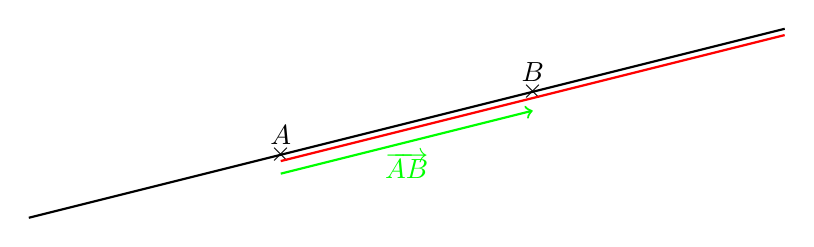
\begin{tikzpicture}[scale=0.8]
\coordinate (A) at (0, 0) ; 
\coordinate (B) at (4, 1) ; 
% Le coef directeur est 1/4 et le vecteur directeur (4 ; 1)     
   
\coordinate (A2) at (0, 0) ; 
\coordinate (B2) at (3, 1) ; 
\coordinate (A3) at (0, 0) ; 
\coordinate (B3) at (3, 1) ; 
\draw[thick] (-4,-1)  -- (8,2) ;
\draw (0,0) node {$\times$} ; \draw (0,0) node [above] {$A$} ;
\draw (4,1) node {$\times$} ; \draw (4,1) node [above] {$B$} ;
    
\draw[thick,red] (0,-0.1)  -- (8,1.9) ;
\draw[thick,green, ->] (0,-0.3)  -- node[midway,below, green]{$ \overrightarrow{AB}$} (4,0.7) ;
\end{tikzpicture}

\begin{itemize}
\item[*] La direction de droite est la direction de la droite $ \left(AB\right) $
\item[*] Le sens sur cete direction est le sens de A vers B, c'est-à-dire le sens de la demi-droite $\left[AB\right)$
\item[*] Le nombre réel positif est la longueur du segment $\left[AB\right]$, c'est-à-dire la distance AB.
\end{itemize}

\subsection{Égalité de 2 vecteurs}

Soient $\overrightarrow{AB}$ et $\overrightarrow{CD}$ deux vecteurs. \\

$\overrightarrow{AB}=\overrightarrow{CD}$ si et seulement si :
\begin{itemize}
\item[*] La direction $(AB) =$ la direction de $(CD)$, c'est-à-dire $(AB)//(CD)$.
\item[*] Le sens de $\left[AB\right) =$ le sens de $\left[CD\right)$
\item[*] La longueur de $[AB] =$ la longueur de $[CD]$
\end{itemize}

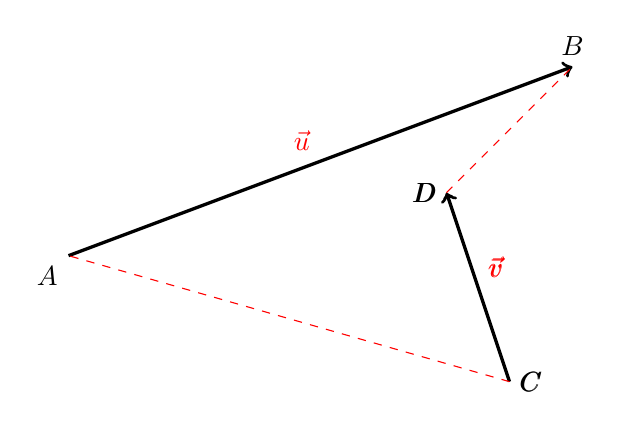
\begin{tikzpicture}[scale=0.8]
\draw[color=black,very thick, ->]
% A(0,0) L'étiquette est à côté de du point.
% Le nom du vecteur u est au dessus à gauche du milieu du trait épais 
(0,2) node [below left] {$A$} --  node[color=red, midway,above left]{$\vec{u}$}
% Le + signifie la translation 
+(8,3) node [above] {$B$} ;
\draw[color=black,very thick,->] (7,0) node [right] {$C$} --  node[color=red, above right]{$\vec{v}$} +(-1,3) node [left] {$D$} ;
\draw[color=black,->] (7,0) node [right] {$C$} --  node[color=red, above right]{$\vec{v}$} +(-1,3) node [left] {$D$} ;
\draw[color=red,dashed] (7,0)  -- (0,2) ;
\draw[color=red,dashed] (6,3)  -- (8,5) ;
\end{tikzpicture}\\
$\overrightarrow{AB} \neq \overrightarrow{CD}$ car $(AB)$ et $(CD)$ ne sont pas parralèles

\newpage



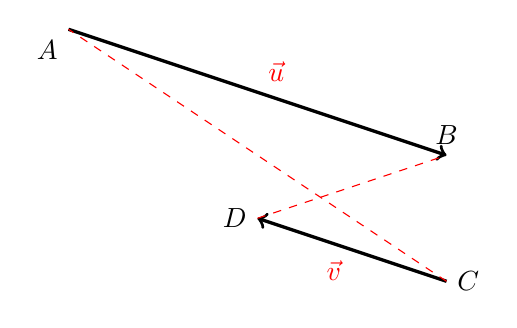
\begin{tikzpicture}[scale=0.8]
\draw[color=black,very thick, ->]
(0,4) node [below left] {$A$} --  node[color=red, midway,above right]{$\vec{u}$}+(6,-2) node [above] {$B$} ;
\draw[color=black,very thick,->] (6,0) node [right] {$C$} --  node[color=red, below left]{$\vec{v}$} +(-3,1) node [left] {$D$} ;
\draw[color=red,dashed] (6,0)  -- (0,4) ;
\draw[color=red,dashed] (3,1)  -- (6,2) ;
\end{tikzpicture}\\


$\overrightarrow{AB} \neq \overrightarrow{CD}$ car $(AB) // (CD)$ mais le sens de $[AB) \neq$ le sens de $[CD)$.

\vspace{1cm}

\begin{tikzpicture}[scale=0.8]
\draw[color=black,very thick, ->]
(5,5) node [below left] {$A$} --  node[color=red, midway,above left]{$\vec{u}$}+(-4,-2) node [above] {$B$} ;
\draw[color=black,very thick,->] (9,5) node [right] {$C$} --  node[color=red, below right]{$\vec{v}$} +(-9,-5) node [left] {$D$} ;
\draw[color=red,dashed] (0,0)  -- (1,3) ;
\draw[color=red,dashed] (5,5)  -- (9,5) ;
\end{tikzpicture}\\

$\overrightarrow{AB} \neq \overrightarrow{CD}$ car $(AB) // (CD)$, le sens de $[AB) = $ le sens de $[CD)$, mais $AB \neq CD$.

\vspace{1cm}

\begin{tikzpicture}[scale=0.8]
\draw[color=black,very thick, ->]
(0,2) node [above left] {$A$} --  node[color=red, midway,above left]{$\vec{u}$}+(8, 2) node [above] {$B$} ;
\draw[color=black,very thick,->] (0,0) node [left] {$C$} --  node[color=red, below right]{$\vec{v}$} +(8, 2) node [right] {$D$} ;
\draw[color=red,dashed] (0,0)  -- (0, 2) ;
\draw[color=red,dashed] (8,2)  -- (8, 4) ;
\end{tikzpicture}\\

$\overrightarrow{AB} = \overrightarrow{CD}$ car $(AB) // (CD)$, le sens de $[AB) = $ le sens de $[CD)$ et $AB = CD$.

$\overrightarrow{u} =\overrightarrow{AB} = \overrightarrow{CD}$

En rouge, le quadrilatère ABDC.

$\overrightarrow{AB} = \overrightarrow{CD} \Longleftrightarrow$ ABDC est un parallélogramme.

Remarques :
\begin{itemize}
\item[*] {\Large $\Longleftrightarrow$} se lit : \og  équivalent à \fg , ou \og  si et seulement si \fg
\item[*] Si $\overrightarrow{AB} = \overrightarrow{CD}$, et ABDC est un parallélogramme, on a aussi :
\begin{itemize}
\item[*]$\overrightarrow{BA} = \overrightarrow{DC}$
\item[*]$\overrightarrow{AC} = \overrightarrow{BD}$
\item[*]$\overrightarrow{CA} = \overrightarrow{DB}$
\end{itemize}
\end{itemize}

\newpage

\subsection{Axiome fondamental}

Soit O un point. 

Soit $\overrightarrow{u}$ un vecteur.

\begin{tikzpicture}[scale=0.8]
\tkzDefPoint [label=left:$O$](0,0){O}
\tkzDrawPoint[size=10,color=black](O)

	\coordinate (M) at (6, 2) ; 

    \draw[very thick,->] (0,0) --  (6,2) node [above] {$M$}  ;
    \draw[thick, ->] (0,-2) -- node[midway,above]{$\vec{u}$} +(6,2);
\end{tikzpicture} \\

Il existe un point M et un seul tel que $\overrightarrow{OM} = \overrightarrow{u}$

\subsection{Addition de vecteurs}

Soit $\vec{u}$ et $\vec{v}$ deux vecteurs.

\begin{tikzpicture}[scale=0.8]
    \coordinate (A) at (0, 0) ; 
    \coordinate (B) at (2, 4) ; 
    \coordinate (C) at (7, 4) ; 	
    \coordinate (C) at (11, 4) ; 	

  \draw[thick,green, ->] (0,0)  --  node[midway,above, green]{$\vec{u}$} +(2,4);
    \draw[thick, ->] (7,4) -- node[midway,above]{$\vec{v}$} +(4,0);

\end{tikzpicture} \\

\subsubsection{Méthode mathématique}

\begin{tikzpicture}[scale=0.8]
    \coordinate (A) at (0, 0) ; 
    \coordinate (B) at (2, 4) ; 
    \coordinate (C) at (2, 4) ; 	
    \coordinate (C) at (6, 4) ; 	
    \draw[thick,green, ->] (0,0) node [below left, black] {$A$} --  node[midway,above, green]{$\vec{u}$} +(2,4) node [above, black] {$B$} ;
    \draw[thick, ->] (2,4) -- node[midway,above]{$\vec{v}$} +(4,0) node [above] {$C$} ;
    \draw[thick,red, ->] (0,0) --  node[midway,below right]{$\vec{u}+\vec{v}$} +(6,4);
\end{tikzpicture}

$\vec{u} + \vec{v} = \overrightarrow{AC}$ \\

$\overrightarrow{AB} + \overrightarrow{BC} = \overrightarrow{AC}$ \\

Ceci s'appelle la \textbf{Relation de Chasles} (Michel Chasles est un mathématicien français (1793-1880)).

\subsubsection{Méthode physique}

\begin{tikzpicture}[scale=0.8]
    \coordinate (A) at (0, 0) ; 
    \coordinate (B) at (2, 4) ; 
    \coordinate (C) at (2, 4) ; 	
    \coordinate (C) at (6, 4) ; 	
    \draw[thick,green, ->] (0,0) node [below left, black] {$O$} --  node[midway,above, green]{$\vec{u}$} +(2,4) node [above, black] {$A$} ;
    \draw[dashed] (2,4) --  +(4,0) node [above] {$C$} ;
    \draw[thick, ->] (0,0) -- node[midway,above]{$\vec{v}$} +(4,0) node [above] {$B$} ;
    \draw[thick,red, ->] (0,0) --  node[midway,below right]{$\vec{u}+\vec{v}$} +(6,4);
    \draw[dashed] (4,0) --  +(2,4) node [above] {$C$} ;
\end{tikzpicture} 

$\vec{u} + \vec{v} = \overrightarrow{OC}$ \\

$\overrightarrow{OA} + \overrightarrow{OB} = \overrightarrow{OC}$ \\

Ceci est \textbf{la règle du parallélogramme}. Le vecteur
$\overrightarrow{OC}$ s'appelle \textbf{la résultante des forces}. \\

\subsection{Conséquences de la relation de Chasles}

\subsubsection{Le vecteur nul}

Soit A un point. \\

Combien vaut le vecteur $\overrightarrow{AA}$ ? \\


$\overrightarrow{AA} + \overrightarrow{AB} = \overrightarrow{AB}$

$ x + a = a $

$ x = 0 $.

Donc $\overrightarrow{AA} = \overrightarrow{0}$ (<-- vecteur nul) \\

\subsubsection{L'opposé d'un vecteur}

Soient A et B deux points.


Combien vaut le vecteur $\overrightarrow{BA}$ ? \\


$\overrightarrow{AB} + \overrightarrow{BA} = \overrightarrow{AA}$

$\overrightarrow{AB} + \overrightarrow{BA} = \overrightarrow{0}$

$ a + x = 0 $

$ x = - a $

Donc $\overrightarrow{BA} = -\overrightarrow{AB}$ (<-- opposé de $\overrightarrow{AB}$

\subsubsection{Soustraction de deux vecteurs}

\begin{tikzpicture}[scale=0.8]
 \draw[thick,green, ->] (0,0)  --  node[midway,below right , green]{$\vec{u}$} +(2,4);
    \draw[thick, ->] (7,4) -- node[midway,above]{$\vec{v}$} +(4,0);
\end{tikzpicture} 

$\overrightarrow{u} - \overrightarrow{v} = \overrightarrow{u}+\left(-\overrightarrow{v}\right)$

\begin{tikzpicture}[scale=0.8]

    \draw[thick, <-] (0,0) -- node[midway,above]{$-\vec{v}$} +(-4,0) node [above] {$C$} ;
    \draw[thick,green, ->] (-2,-4) --  node[midway,below right, green]{$\vec{u}$} +(2,4);
    \draw[thick,red, ->] (-2,-4) --  node[midway,below left]{$\vec{u}-\vec{v}$} +(-2,4);
\end{tikzpicture} 

\subsection{Multiplication d'un vecteur par un nombre réel}

Soit $\overrightarrow{u}$ un vecteur.

Soit $\lambda$ un nombre réel. 

\begin{tikzpicture}[scale=0.8]
 \draw[thick,green, ->] (0,0)  --  node[midway,below right , green]{$\vec{u}$} +(2,4);
\end{tikzpicture} 

Le produit du vecteur $\overrightarrow{u}$ par le nombre réel $\lambda$ est le vecteur noté $\lambda\overrightarrow{u}$ défini par : 

-- La direction de $\left(CD\right) = $ la direction de $\left(AB\right)$, c'est-à-dire $\left(AB\right) // \left(CD\right) $ \\

\begin{tabular}{l|l}

$\lambda > 0 $ & $\lambda < 0$ \\
* Le sens de $\left[CD\right) $ & * le sens de $\left[AB\right) $ \\ 
 $ CD = \lambda AB $ & $ CD = -\lambda AB$ \\
\end{tabular}


\subsubsection{Exemple \no 1}

$\lambda = 3 $

\begin{tikzpicture}[scale=0.6]
\draw[thick,green, ->] (1,2) node [below left] {$A$} --  node[midway,above left, green]{$\vec{u}$} +(1,2) node [above] {$B$} ;
    
\draw[thick,green, ->] (3,0) node [below] {$C$} --  node[midway, below right, green]{$3\vec{u}$} +(3,6) node [above ] {$D$} ;
\draw (4,2) node {$-$} ; \draw (5,4) node {$-$} ; 
\end{tikzpicture}

\subsubsection{Exemple \no 2}

$\lambda = -2 $

\begin{tikzpicture}[scale=0.8]
\draw[thick, ->] (1,2) node [below left] {$A$} --  node[midway,above left]{$\vec{u}$} +(1,2) node [above] {$B$} ;
    
\draw[thick, <-] (3,0) node [below] {$D$} --  node[midway, below right]{$-2\vec{u}$} +(2,4) node [above ] {$C$} ;
\draw (4,2) node {$-$} ; 
\end{tikzpicture}

Et si $\lambda = 0$ ? \\

Alors $0\overrightarrow{u} = \overrightarrow{0}$

\subsection{Notions d'espace vectoriel}

Soient $\overrightarrow{u}$, $\overrightarrow{v}$, et  $\overrightarrow{w}$ trois vecteurs.

Soient $\lambda$ et $\mu$ deux nombres réels. \\

\subsubsection{Relations avec des vecteurs}

\begin{itemize}
\item[*] $\overrightarrow{u} + \overrightarrow{v}$ = $\overrightarrow{v} + \overrightarrow{u}$
\item[*] $\overrightarrow{u} + \left(\overrightarrow{v} + \overrightarrow{w} \right) = \left( \overrightarrow{u} + \overrightarrow{v} \right) + \overrightarrow{w}$
\item[*] $\overrightarrow{u} + \overrightarrow{0} = \overrightarrow{u}$
\item[*] $\overrightarrow{u} + \left(-\overrightarrow{u}\right) = \overrightarrow{0}$
\end{itemize}

\subsubsection{Relations avec des vecteurs et des nombres réels}

\begin{itemize}
\item[*]$1\overrightarrow{u} = \overrightarrow{u}$
\item[*]$\lambda\left(\mu \overrightarrow{u} \right) = \left(\lambda\mu\right)\overrightarrow{u}$
\item[*] $\lambda \times \left( \overrightarrow{u} + \overrightarrow{v}\right) = \lambda \overrightarrow{u} + \lambda \overrightarrow{v}$
\item[*] $\left(\lambda + \mu \right) \overrightarrow{u} = \lambda \overrightarrow{u} + \mu \overrightarrow{u}$
\end{itemize}

\newpage 
\subsection{Vecteurs colinéaires}

\subsubsection{Définition}

Soient $\overrightarrow{u}$ et $\overrightarrow{v}$ deux vecteurs, avec $\overrightarrow{u} \neq \overrightarrow{0}$.

$\overrightarrow{v}$ est colinéaire à $\overrightarrow{u}$ si et seulement si : il existe $\lambda \in \R$ tel que $\overrightarrow{v} = \lambda\overrightarrow{u}$ \\

Exemple :

\begin{tikzpicture}[scale=0.6]
% A(0,0) L'étiquette est à côté de du point.
% Le nom du vecteur u est au dessus à gauche du milieu du trait épais 
\draw[thick, ->] (0,0) node [below left] {$A$} --  node[midway,above left]{$\vec{u}$}
% Le + signifie la translation 
+(2,2) node [above] {$B$} ;

% D(3,0)
\draw[thick, ->] (3,0) node [below] {$D$} --  node[midway, below right]{$\vec{v}$} +(6,6) node [above ] {$C$} ;
% On place deux petites marques pour montrer v = 3u
\draw (5,2) node {$\setminus$} ; 
\draw (7,4) node {$\setminus$} ; 
\end{tikzpicture}

$\overrightarrow{v}$ est coliénaire à $\overrightarrow{u}$ car  $\overrightarrow{v} = 3 \overrightarrow{u}$. \\

\textbf{Remarque}

$\overrightarrow{0}$ est colinéaire à tous les vecteurs du plan. En effet, pour tout vecteur $\overrightarrow{u}$, on a $\overrightarrow{0} = 0 \overrightarrow{u}$ \\

Soient $\overrightarrow{u} \neq \overrightarrow{0}$ et $\overrightarrow{v} \neq \overrightarrow{0}$ tels que $\overrightarrow{v}$ est colinéaire à $\overrightarrow{u}$. Il existe $ \lambda \in \R $ tel que $\overrightarrow{v} = \lambda\overrightarrow{u}$ avec $\lambda \neq 0 $.

On a donc $\overrightarrow{u} = \dfrac{1}{\lambda}\overrightarrow{v}$ et non $\overrightarrow{u} = \dfrac{\overrightarrow{v}}{\lambda}$

\subsubsection{Syntaxe}

On dit que $\overrightarrow{u}$ et $\overrightarrow{v}$ sont colinéaires, ou que $\overrightarrow{v}$ est colinéaire à  $\overrightarrow{u}$. 

\subsubsection{À retenir}

Soient $\overrightarrow{u}$ et $ \overrightarrow{v} $ deux vecteurs 
colinéaires. Il existe un nombre $\lambda \in \R $ tel que $ \overrightarrow{v} = \lambda \overrightarrow{u} $ avec $ \lambda \neq 0$ \\

\begin{tabular}{c|c}

Si $\lambda > 0 $ & Si $\lambda < 0$ \\
$\overrightarrow{u}$ et $\overrightarrow{v}$ sont colinéaires et de même sens & $\overrightarrow{u}$ et $\overrightarrow{v}$ sont colinéaires et de sens contraires.

\end{tabular}

\subsubsection{Points alignés}

Soient A, B et C trois points alignés.\\

A, B et C sont alignés si et seulement si : $ \overrightarrow{AB}$ et $\overrightarrow{AC}$ sont colinéaires.

% Points alignés
\begin{tikzpicture}[scale=0.8]
\draw[thick, ->] (0,0) --  +(5,3)  ;
 \tkzText(0.5,0.3){\textcolor{black}{$\times$}}  % cf ci-dessus
 \tkzText(.5,.7){\textcolor{black}{A}}
 \tkzText(1.5,.9){\textcolor{black}{$\times$}}  % cf ci-dessus
 \tkzText(1.5,1.3){\textcolor{black}{B}}
 \tkzText(4,2.4){\textcolor{black}{$\times$}}  % cf ci-dessus
 \tkzText(3.9,2.8){\textcolor{black}{C}}
\end{tikzpicture}

A, B et C sont alignés car $\overrightarrow{AB}$ et $\overrightarrow{AC}$ sont colinéaires.

\subsubsection{Droites parallèles}

Soient $\left(AB\right)$ et $\left(CD\right)$ deux droites : \\

$\left(AB\right)$ et $\left(CD\right)$ sont parallèles si et seulement si : $\overrightarrow{AB}$ et $\overrightarrow{AC}$ sont colinéaires.

% Droites //
\begin{tikzpicture}[scale=0.8]
% A(0,0) 
\draw[-] (-2,-1) -- +(8,4) ;
\draw[very thick, ->] (0,0) node [below left] {$A$} -- +(4,2) ;
\draw (0,0) node {$\setminus$} ; 
%\draw (2,1) node {$-$} ; 
%\draw (4,2) node {$-$} ; 
%\draw (4,2) node {$\times$} ; 
%\draw (4,2) node {$\times$} ; 
\draw (4,2) node [above]{$B$} ; 
% D(3,0)
\draw[-] (2,-1) -- +(8,4) ;
\draw[very thick, ->] (4,0) node [below] {$C$} --   +(1, .5) node [above ] {$D$} ;
\end{tikzpicture}

$\left(AB\right) // \left(CD\right) $ car $\overrightarrow{CD} = \dfrac{1}{4} \overrightarrow{AB}$

\subsection{Milieu d'un segment}

\subsubsection{Définition}

Soient A et B deux points distincts.

Il existe un point I et un seul tel que $\overrightarrow{IA} + \overrightarrow{IB} = \overrightarrow{0}$, c'est-à-dire $\overrightarrow{AI} = \dfrac{1}{2} \overrightarrow{AB} $

I est le milieu de $\left[AB\right]$

% milieu d'un segmeny
\begin{tikzpicture}[scale=0.8]
\draw[very thick, -] (-.2,0) --  +(6.4,0)  ;
 \tkzText(0,0){\textcolor{black}{$|$}}  % cf ci-dessus
 \tkzText(0,.5){\textcolor{black}{A}}
 \tkzText(3,0){\textcolor{black}{$|$}}  % cf ci-dessus
 \tkzText(3,.5){\textcolor{black}{$I$}}
 \tkzText(6,0){\textcolor{black}{$|$}}  % cf ci-dessus
 \tkzText(6,.5){\textcolor{black}{$B$}}
\draw (1.47,0.09) -- (1.47,-0.09);
\draw (1.54,0.09) -- (1.54,-0.09);
\draw (4.47,0.09) -- (4.47,-0.09);
\draw (4.54,0.09) -- (4.54,-0.09);
\end{tikzpicture}

\subsubsection{Démonstration}

$\overrightarrow{IA} + \overrightarrow{IB} = \overrightarrow{0} $\\

$ \overrightarrow{IA} + \left(\overrightarrow{IA} + \overrightarrow{AB}\right) = \overrightarrow{0} $\\

$ 2\overrightarrow{IA} + \overrightarrow{AB} = \overrightarrow{0} $\\

$ 2\overrightarrow{IA} = -\overrightarrow{AB} $\\

$\overrightarrow{IA} = -\dfrac{1}{2} \overrightarrow{AB} $\\

$ \overrightarrow{AI} = \dfrac{1}{2} \overrightarrow{AB} $\\

\newpage 

\subsection{Centre de gravité d'un triangle}

Soient A, B et C trois points non-alignés.

Il existe un point G et un seul tel que $\overrightarrow{GA} + \overrightarrow{GB} + \overrightarrow{GC} = \overrightarrow{0} $, c'est-à-dire $\overrightarrow{AG} = \dfrac{1}{3} \overrightarrow{AB} + \dfrac{1}{3} \overrightarrow{AC} $ \\

\subsubsection{Démonstration}

$\overrightarrow{GA}+\overrightarrow{BG}+\overrightarrow{GC}=\overrightarrow{0}$\\

$ \overrightarrow{GA} + \left(\overrightarrow{GA} + \overrightarrow{AB} \right) + \left(\overrightarrow{GA} + \overrightarrow{AC}\right) = \overrightarrow{0} $\\

$ 3\overrightarrow{GA} = -\overrightarrow{AB} - \overrightarrow{AC} $\\

$ \overrightarrow{GA} = -\dfrac{1}{3} \overrightarrow{AB} - \dfrac{1}{3} \overrightarrow{AC} $\\

$ \overrightarrow{AG} = \dfrac{1}{3} \overrightarrow{AB} + \dfrac{1}{3} \overrightarrow{AC} $\\

\subsubsection{Propriété fondamentale}

\begin{tikzpicture}[scale=0.5]
\coordinate (G) at (0.2,-0.07) ; 

\draw (6,8) node [above] {$A$} --  (-8.7,-5) node [left] {$B$} -- (8.7,-5) node [right] {$C$}-- (6, 8) ; 
\draw (6,8) -- (0,-5) node [below] {$A'$} ;
\draw (-8.7,-5) -- (7.4,1.5) node [right] {$B'$} ;
\draw (8.7,-5) -- (-1.3,1.5) node [left] {$C'$} ;
\draw (2,-0.7) node [below right] {$G$} ; 

\draw [very thick, ->](6,8) -- +(-14.7/3, -13/3) ; % 1/3 de vec(AB)
\draw [dashed](2, -0.7) -- +(-2.7/3, 13/3) ;       % 1/3 de vec(-AC)
\draw [very thick, ->](6,8) -- +(2.7/3, -13/3) ;   % 1/3 de vec(AC)
\draw [dashed](2, -0.7) -- +(14.7/3, 13/3) ;       % 1/3 de vec(-AB)
\draw [very thick, ->](6,8) -- +(-12/3, -26/3) ;   % 2/3 de vec(AA')
\draw [very thick, red] (4,7.3/2) node {\bf ---} ; % 1/2 de AG 

\end{tikzpicture}

Soit A' le milieu de $\left[BC\right]$

$ \overrightarrow{AG} = \dfrac{1}{3} \overrightarrow{AB} + \dfrac{1}{3} \overrightarrow{AC} $\\

$ \overrightarrow{AG} = \dfrac{1}{3} \left(\overrightarrow{AA'} + \overrightarrow{A'B}\right) + \dfrac{1}{3} \left(\overrightarrow{AA'} + \overrightarrow{A'C} \right) $ \\

$ \overrightarrow{AG} = \dfrac{2}{3} \overrightarrow{AA'} + \dfrac{1}{3} \underbrace{\left(\overrightarrow{A'B} + \overrightarrow{A'C}\right)}_{= \overrightarrow{0} \textrm {car} A' \textrm {est le milieu de} \left[BC\right]} $\\

$ \overrightarrow{AG} = \dfrac{2}{3} \overrightarrow{AA'} $\\

On aussi, avec B' le milieu de $\left[AC\right]$, on a $\overrightarrow{BG} = \dfrac{2}{3} \overrightarrow{BB'} $, et avec C' le milieu de $\left[AB\right]$, on a $\overrightarrow{CG} = \dfrac{2}{3} \overrightarrow{CC'} $

Les trois médianes du triangle sont concourantes en un point, ici G.

\newpage

\subsection{Exercices}

\subsubsection{Exercice \no 0}

Soit ABC un triangle. \\

1. Soit A' le milieu de $\left[BC\right]$. Montrer que $\overrightarrow{AB} + \overrightarrow{AC} = 2\overrightarrow{AA'}$. \\

2. Soient I le milieu de $\left[AB\right]$ et J le milieu de $\left[AC\right]$. Montrer que $\overrightarrow{IJ} = \dfrac{1}{2} \overrightarrow{BC}$.

\begin{tikzpicture}[scale=0.3]
\draw (6,8) node [above] {$A$} --  (-8.7,-5) node [left] {$B$} -- (8.7,-5) node [right] {$C$} -- (6, 8) ; 
\draw [red,->](6,8) -- +(-12, -26) node [midway,below right] {$A'$} node [below] {$G$} ;

\draw [green, ->] (-1.3, 1.5) node [left] {$I$} -- (7.4,1.5) node [right] {$J$} ;

\draw [dashed] (-8.7, -5) -- +(2.7,-13) ;     % ie vec(AC)
\draw [dashed] (8.7, -5) -- +(-14.7,-13) ;     % ie vec(AB)

\end{tikzpicture}

1. $\overrightarrow{AB} + \overrightarrow{AC} = \left(\overrightarrow{AA'} + \overrightarrow{A'B}\right) + \left(\overrightarrow{AA'} + \overrightarrow{A'C}\right) $\\

$ \overrightarrow{AB} + \overrightarrow{AC} = 2 \overrightarrow{AA'} + \underbrace{\overrightarrow{A'B} + \overrightarrow{A'C}}_{= \overrightarrow{0} \textrm{ car } A' \textrm { est le milieu de } \left[BC\right]} $

$ \overrightarrow{AB} + \overrightarrow{AC} = 2 \overrightarrow{AA'} $\\

Donc les diagonales du parallélogramme se coupent en leur milieu. \\

2. $ \overrightarrow{IJ} = \overrightarrow{IA} + \overrightarrow{AJ} $\\

$ \overrightarrow{IJ} = -\overrightarrow{AI} + \overrightarrow{AJ} $\\

$ \overrightarrow{IJ} = -\dfrac{1}{2} \overrightarrow{AB} + \dfrac{1}{2} \overrightarrow{AC} $\\

$ \overrightarrow{IJ} = \dfrac{1}{2} \left(-\overrightarrow{AB} + \overrightarrow{AC} \right) $\\

$ \overrightarrow{IJ} = \dfrac{1}{2} \left(\overrightarrow{BA} + \overrightarrow{AC}\right) $\\

$ \overrightarrow{IJ} = \dfrac{1}{2} \overrightarrow{BC} $
\newpage
\subsubsection{Un superbe exercice}

Soit ABC un triangle.

Soit A' le milieu de $\left[BC\right]$.

Soit G le centre de gravité de ABC.

Soit M un point quelconque.\\

1. Montrer que $ \overrightarrow{MA} + \overrightarrow{MB} + \overrightarrow{MC} = 3\overrightarrow{MA} + 2\overrightarrow{AA'}$

2. Montrer que $ \overrightarrow{MA} + \overrightarrow{MB} + \overrightarrow{MC} = 3\overrightarrow{MG} $

\begin{tikzpicture}[scale=0.7]
\draw (0,8) node [left] {$A$} --  (8,4) node [below] {$B$} -- (12,16) node [right] {$C$} -- (0, 8) ; 
\draw [thick, ->] (0,8) -- +(10,2) node [right] {$A'$} ;   
\draw [dashed] (8,4) -- +(-2,8) ;   
\draw [dashed] (12,16) -- +(-8,-10);   
\draw (20/3, 18/2) node [below] {$G$} ; 

\draw [blue, ->] (0,12) node [left] {$M$} -- +(0,-4) ; 
\draw [green, ->] (0,12) node [left] {$M$} -- +(8,-8) ; 
\draw [violet, ->] (0,12) node [left] {$M$} -- +(12,4) ; 

\draw [thick, blue, ->] (0,12) node [left] {$M$} -- +(0,-12) ; 
\draw [black, ->] (0,0) --  +(20,4) ; 
\draw [red, ->] (0,12) -- +(20, -8) ; 

\draw [green, ->] (0,8) -- +(8,-8) ; 
\draw [violet, ->] (8,0) -- +(12,4) ; 

\end{tikzpicture}

\vspace*{1cm}

\begin{enumerate}


\item $\overrightarrow{MA} + \overrightarrow{MB} + \overrightarrow{MC} = \overrightarrow{MA} + \left(\overrightarrow{MA} + \overrightarrow{AA'} + \overrightarrow{A'B}\right) + \left(\overrightarrow{MA} + \overrightarrow{AA'} + \overrightarrow{A'C}\right) $\\

$ \overrightarrow{MA} + \overrightarrow{MB} + \overrightarrow{MC} = 3\overrightarrow{MA} + 2\overrightarrow{AA'} +$\hspace*{-0.94cm}$ \underbrace{\overrightarrow{A'B} + \overrightarrow{A'C}}_{= \overrightarrow{0} \textrm{ car } A' \textrm{ est le milieu de } \left[BC\right]}$ 

\item  $ \overrightarrow{MA} + \overrightarrow{MB} + \overrightarrow{MC} = \left(\overrightarrow{MG} + \overrightarrow{GA}\right) + \left(\overrightarrow{MG} + \overrightarrow{GB} \right) + \left(\overrightarrow{MG} + \overrightarrow{GC} \right) $\\

$ \overrightarrow{MA} + \overrightarrow{MB} + \overrightarrow{MC} =
3\overrightarrow{MG} + $\hspace*{-1.8cm}$\underbrace{\overrightarrow{GA} + \overrightarrow{GB} + \overrightarrow{GC}}_{=\overrightarrow{0} \textrm{car } G \textrm { est le centre de gravité du triangle } ABC} $

\end{enumerate}
\newpage
\subsubsection{Exercice \no 1}

Soit ABC un triangle.

1. Construire les points M et N définis par : \\

\begin{itemize}
\item[*] $ \overrightarrow{AM} = \dfrac{1}{3} \overrightarrow{AB} + \overrightarrow{AC} $ \\
\item[*] $ \overrightarrow{AN} = 2\overrightarrow{AB} - \dfrac{2}{3} \overrightarrow{AC} $ \\
\end{itemize}

2. Exprimer $\overrightarrow{MN}$ en fonction de $\overrightarrow{AB}$ et de $\overrightarrow{AC}$. \\

3. Montrer que les droites $\left(MN\right)$ et $\left(BC\right)$ sont parallèles. \\

\begin{enumerate}


\item ~   % Le tilde (~) est nécessaire pour que le numéro précède la figure

\begin{tikzpicture}[scale=0.2]
\draw [color=black] (0,0) node [left] {$B'$} --  (6,12) node [below] {$B$} -- (12,24) node [right] {$A$} ; 
\draw [color=violet] (12,24) -- +(+12, -12)  node [right] {$C$} ; 
\draw [color=black] (24,12) -- (6, 12) ; 
\draw (8,16) node {$-$} ;   
\draw (16,20) node {$-$} ;   
\draw (20,16) node {$-$} ;   

\draw [color=green, very thick, ->] (12, 24) -- +(-2,-4) ; 
\draw [color=violet, thick, ->] (10, 20) -- +(12,-12) node [below] {$M$} ; 
\draw [color=magenta, thick, ->] (0, 0) -- +(-8,8) node [below] {$N$} ; 

\draw [color=red, thick, -] (-10, 12) -- (26,12) ; 
\draw [color=red, thick, -] (-10, 8) -- (26,8) ; 

\end{tikzpicture}\\


\item  $\overrightarrow{MN} = \overrightarrow{MA} + \overrightarrow{AN} $\\

$ \overrightarrow{MN} = -\overrightarrow{AM} + \overrightarrow{AN} $\\

$ \overrightarrow{MN} = -\dfrac{1}{3} \overrightarrow{AB} - \overrightarrow{AC} + 2\overrightarrow{AB} - \dfrac{2}{3} \overrightarrow{AC} $\\

$ \overrightarrow{MN} = \dfrac{5}{3} \overrightarrow{AB} - \dfrac{5}{3} \overrightarrow{AC} $\\

$ \overrightarrow{MN} = \dfrac{5}{3} \left(\overrightarrow{AB} - \overrightarrow{AC}\right) $\\

\item  $ \overrightarrow{MN} = \dfrac{5}{3} \left(\overrightarrow{AB} - \overrightarrow{AC} \right)$\\

$ \overrightarrow{MN} = \dfrac{5}{3} \left(\overrightarrow{AB} + \overrightarrow{CA} \right)$\\

$ \overrightarrow{MN} = \dfrac{5}{3} \left(\overrightarrow{CA} + \overrightarrow{AB} \right)$\\

$ \overrightarrow{MN} = \dfrac{5}{3} \left(\overrightarrow{CB} \right)$\\

$ \overrightarrow{MN} = -\dfrac{5}{3} \left(\overrightarrow{BC}\right)$\\

Les vecteurs $\overrightarrow{MN}$ et $\overrightarrow{BC}$ sont colinéaires, donc $\left(MN\right)//\left(BC\right)$
\end{enumerate}
\newpage
\subsubsection{Exercice \no 2}

Soit ABC un triangle.

\begin{enumerate}


\item  Construire les points I, J et K définis par :

\begin{itemize}
\item[*] $\overrightarrow{AI} = \dfrac{1}{3} \overrightarrow{AB}$\\
\item[*] $\overrightarrow{BJ} = \dfrac{1}{2} \overrightarrow{BA} - \dfrac{1}{4} \overrightarrow{BC}$\\
\item[*] $\overrightarrow{CK} = -\overrightarrow{AB} - \dfrac{1}{2} \overrightarrow{BC}$\\
\end{itemize}

\item  Exprimer $\overrightarrow{IJ}$ fonction de $\overrightarrow{AB}$ et de $ \overrightarrow{BC}$. 

Puis, exprimer $\overrightarrow{IK}$ en fonction de $\overrightarrow{AB}$ et de $\overrightarrow{BC}$.

\item  Montrer que les points I, J et K sont alignés.

\end{enumerate}

~

\begin{enumerate}

\item  ~ % (Garder là le tilde) Exercice n°2 

\begin{tikzpicture}[scale=0.3]

\draw [->] (0, 0) node [left] {$B$} --  +(12, 0) node [below] {$C$} ; 
\draw [color=green, <-] (0, 0) -- +(3, 9) node [above] {$A$} ; 
\draw      (3, 9) --  (12, 0); 

\draw [very thick, color=green, ->] (3, 9) -- +(-1, -3) node [left] {$I$} ; 
\draw [->] (3/2, 9/2) -- +(-3, 0) node [above] {$J$} ; 
\draw [color=green, ->] (12, 0) -- +(3, 9); 
\draw [color=violet, ->] (15, 9) -- +(-6, 0) node [above] {$K$} ; 
\draw [color=red] (2, 6) -- +(14, 6) -- +(-7, -3); 

\end{tikzpicture}\\

\begin{multicols}{2}


\item  {\small $\overrightarrow{IJ} = \overrightarrow{IA} + \overrightarrow{AB} + \overrightarrow{BJ} $\\

$\overrightarrow{IJ} = -\dfrac{1}{3} \overrightarrow{AB} + \overrightarrow{AB} + \dfrac{1}{2} \overrightarrow{BA} - \dfrac{1}{4} \overrightarrow{BC} $\\

$\overrightarrow{IJ} = -\dfrac{1}{3} \overrightarrow{AB} + \overrightarrow{AB} - \dfrac{1}{2} \overrightarrow{AB} - \dfrac{1}{4} \overrightarrow{BC} $\\

$ \overrightarrow{IJ} = \dfrac{1}{6} \overrightarrow{AB} - \dfrac{1}{4} \overrightarrow{BC} $\\

Et : $\overrightarrow{IK} = \overrightarrow{IA} + \overrightarrow{AB} + \overrightarrow{BC} + \overrightarrow{CK} $\\

$ \overrightarrow{IK} = -\dfrac{1}{3} \overrightarrow{AB} + \overrightarrow{AB} + \overrightarrow{BC} - \overrightarrow{AB} - \dfrac{1}{2} \overrightarrow{BC} $\\

$ \overrightarrow{IK} = -\dfrac{1}{3} \overrightarrow{AB} + \dfrac{1}{2} \overrightarrow{BC} $\\

\item $\overrightarrow{IK} = \overrightarrow{IB} + \overrightarrow{BC} + \overrightarrow{BA} + \dfrac{1}{2} \overrightarrow{CB} $\\

$ \overrightarrow{IK} = \dfrac{2}{3} \overrightarrow{AB} + \overrightarrow{BC} - \overrightarrow{AB} - \dfrac{1}{2} \overrightarrow{BC} $\\

$ \overrightarrow{IK} = -\dfrac{1}{3} \overrightarrow{AB} + \dfrac{1}{2} \overrightarrow{BC} $\\

On constate que $\overrightarrow{IK} = -2\left(\dfrac{1}{6} \overrightarrow{AB} + \dfrac{1}{2} \overrightarrow{BC}\right) $\\

$ \overrightarrow{IK} = -2\overrightarrow{IJ} $
}\\

Donc les vecteurs $\overrightarrow{IK}$ et $\overrightarrow{IJ}$ sont colinéaires, donc les points I, J et K sont alignés.

\end{multicols} 
\end{enumerate}
\newpage
\subsubsection{Exercice \no 3}

Soit ABC un triangle.

\begin{enumerate}


\item  Construire les points I et J tels que :

\begin{itemize}
\item[*] $\overrightarrow{AI} = -2\overrightarrow{AB}$\\
\item[*] $\overrightarrow{AJ} = - \overrightarrow{AB} + \dfrac{1}{2} \overrightarrow{AC}$\\
\end{itemize}

\item  Montrer que J et le milieu de $\left[IC\right]$
\end{enumerate}



\begin{enumerate}

 \item ~ \\% Exercice n°3 (suite) 
 
\begin{tikzpicture}[scale=.4]

\draw [color=black] (0, 0) node [left] {$B$} --  (6, 6) node [left] {$A$} ; 
\draw [color=green, ->] (6, 6) -- +(4, -6) node [right] {$C$} ; 
\draw (0, 0) --  (10, 0); 
\draw [color=green, ->] (6, 6) -- +(2, -3); 
\draw [color=violet, ->] (6, 6) -- +(12, 12) node [right] {$I$} ; 
\draw [color=red, ->] (10, 0) -- +(8, 18); 
\draw [color=green, ->] (12, 12) -- +(2, -3) node [right] {$J$} ; 
\end{tikzpicture}

\vspace*{1cm}


\item $\overrightarrow{JI} + \overrightarrow{JC} = \left(\overrightarrow{JA} + \overrightarrow{AI}\right) + \left(\overrightarrow{JA} + \overrightarrow{AC}\right) $

$ \overrightarrow{JI} + \overrightarrow{JC} = \overrightarrow{AB} - \dfrac{1}{2} \overrightarrow{AC} + \overrightarrow{AI} +\overrightarrow{AB} - \dfrac{1}{2} \overrightarrow{AC} + \overrightarrow{AC} $

$\overrightarrow{JI} + \overrightarrow{JC} = 2\overrightarrow{AB} + \overrightarrow{AI} $

$ \overrightarrow{JI} + \overrightarrow{JC} = 2\overrightarrow{AB} + \left(-2\right)\overrightarrow{AB} $

$ \overrightarrow{JI} + \overrightarrow{JC} = \overrightarrow{0} $

Donc J est le milieu de $\left[IC\right]$.

\end{enumerate}

\newpage
\subsubsection{Exercice \no 4}

Soit ABC un triangle.

Soient A' le milieu de $\left[BC\right]$, B' le milieu de $\left[AC\right]$, et C' le milieu de $\left[AB\right]$

Soit G le centre de gravité de ABC.

\begin{enumerate}


\item  Exprimer :

\begin{itemize}
\item[*] $\overrightarrow{AB} + \overrightarrow{AC} $ en fonction de $\overrightarrow{AA'}$\\
\item[*] $\overrightarrow{BA} + \overrightarrow{BC}$ en fonction de $\overrightarrow{BB'}$\\
\item[*] $\overrightarrow{CA} + \overrightarrow{CB}$ en fontion de $\overrightarrow{CC'}$\\
\end{itemize}

\item Montrer que $\overrightarrow{AA'} + \overrightarrow{BB'} + \overrightarrow{CC'} = \overrightarrow{0} $

\item  Montrer que $G$ est le centre de gravité du triangle A'B'C'.
\end{enumerate}



\begin{enumerate}

\item ~ 

\begin{tikzpicture}[scale=1]
\draw (0,0) node [left] {$B$} -- (2,4) node [above] {$A$} -- (8,0) node [right] {$C$} -- cycle ;  
\draw [red] (1,2) node [left] {$C'$} -- (5,2) node [right] {$B'$} -- (4,0) node [below] {$A'$} -- cycle ; 
\draw [thick, ->] (2,4) -- (4,0) ; 
\draw [blue, ->] (0,0) -- +(5,2) (4,0) -- +(5,2) ; 
\draw [green, ->] (8,0) -- +(-7,2) (9,2) -- +(-7,2) ; 
\end{tikzpicture}


 $\overrightarrow{AB} + \overrightarrow{AC} = \left(\overrightarrow{AA'} + \overrightarrow{A'B}\right) + \left(\overrightarrow{AA'} + \overrightarrow{A'C}\right) $\\

$ \overrightarrow{AB} + \overrightarrow{AC} = 2\overrightarrow{AA'} + \underbrace{\overrightarrow{A'B} + \overrightarrow{A'C}}_{= \overrightarrow{0} \textrm { car } A' \textrm { est le milieu de } \left[BC\right]}$\\

$\overrightarrow{AB} + \overrightarrow{AC} = 2\overrightarrow{AA'} $\\

Donc $\overrightarrow{BA} + \overrightarrow{BC} = 2\overrightarrow{BB'} $ et $ \overrightarrow{CA} + \overrightarrow{CB} = 2\overrightarrow{CC'} $\\

\item  $\overrightarrow{AA'} + \overrightarrow{BB'} + \overrightarrow{CC'} = \dfrac{1}{2} \left(\overrightarrow{AB} + \overrightarrow{AC} \right) + \dfrac{1}{2} \left(\overrightarrow{BA} + \overrightarrow{BC} \right) + \dfrac{1}{2} \left( \overrightarrow{CA} + \overrightarrow{CB} \right) $\\

$\overrightarrow{AA'} + \overrightarrow{BB'} + \overrightarrow{CC'} = \dfrac{1}{2} \overrightarrow{AB} + \dfrac{1}{2} \overrightarrow{BA} + \dfrac{1}{2} \overrightarrow{AC} + \dfrac{1}{2} \overrightarrow{CA} + \dfrac{1}{2} \overrightarrow{BC} + \dfrac{1}{2} \overrightarrow{CB} $\\

$ \overrightarrow{AA'} + \overrightarrow{BB'} + \overrightarrow{CC'} = \dfrac{1}{2} \overrightarrow{AA} + \dfrac{1}{2} \overrightarrow{AA} + \dfrac{1}{2} \overrightarrow{BB} $

$ \overrightarrow{AA'} + \overrightarrow{BB'} + \overrightarrow{CC'} = \overrightarrow{0} $\\

\item $\overrightarrow{GA'} + \overrightarrow{GB'} + \overrightarrow{GC'} = \left(\overrightarrow{GA} + \overrightarrow{AA'} \right) + \left(\overrightarrow{GB} + \overrightarrow{BB'} \right) + \left(\overrightarrow{GC} + \overrightarrow{CC'} \right) $\\

$ \overrightarrow{GA'} + \overrightarrow{GB'} + \overrightarrow{GC'} = \underbrace{\overrightarrow{GA} + \overrightarrow{GB} + \overrightarrow{GC}}_{=\overrightarrow{0} \textrm { car } G \textrm { est le centre de gravité de }  ABC} + \underbrace{\overrightarrow{AA'} + \overrightarrow{BB'} + \overrightarrow{CC'}}_{=\overrightarrow{0} \textrm { d'après } 2.} $\\

Donc G est le centre de gravité du triangle A'B'C'.
\end{enumerate}
\newpage
\subsubsection{Exercice \no 5}

Soit ABCD un quadrilatère quelconque.

Soit $O$ le point d'intersection de $\left[AC\right]$ et de $\left[BD\right] $

\begin{enumerate}


\item  Construire les points I, J, K et L tels que 

\begin{itemize}
\item[*]$\overrightarrow{OI} = \overrightarrow{OA} + \overrightarrow{OB} $\\
\item [*]$ \overrightarrow{OJ} = \overrightarrow{OB} + \overrightarrow{OC} $\\
\item [*]$ \overrightarrow{OK} = \overrightarrow{OC} + \overrightarrow{OD} $\\
\item[*] $ \overrightarrow{OL} = \overrightarrow{OD} + \overrightarrow{OA} $\\
\end{itemize}

\item  Montrer que $\overrightarrow{IJ} = \overrightarrow{AC}$.

De même, exprimer $\overrightarrow{LK}$ en fonction de $\overrightarrow{AC}$

\item  Montrer qie IJKL est un parallélogramme.
\end{enumerate}

\begin{enumerate}


\item ~

\begin{tikzpicture}[scale=1]
\draw (1,6) node [left] {$D$} -- (6,12) node [above] {$A$} -- (11, 11) node [right] {$B$} -- (9,3) node [below] {$C$} -- cycle ;  

\draw [green, ->]  (7,9) node [right] {$O$} -- +(4,2) ; 
\draw [blue, ->]   (7,9) -- +(2, -6) ; 
\draw [violet, ->] (7,9) -- +(-6, -3) ; 
\draw [->]         (7,9) -- +(-1,3) ; 

\draw [dashed] (7,9) -- (0,9) ;
\draw [dashed] (7,9) -- (10,14) ;
\draw [dashed] (7,9) -- (13,5) ;
\draw [dashed] (7,9) -- (3,0) ;

\draw [green, ->]  (6,12)  -- +(4,2)   node [above] {$I$} ; 
\draw [blue, ->]   (11,11) -- +(2,-6)  node [right] {$J$} ; 
\draw [violet, ->] (9,3)   -- +(-6,-3) node [below] {$K$} ; 
\draw [->]         (1,6)   -- +(-1,3)  node [left] {$L$} ; 

\draw [red] (10,14) -- ++(3, -9) -- ++(-10, -5) -- ++(-3, 9) -- cycle ; 

\end{tikzpicture}

\item  $\overrightarrow{IJ} = \overrightarrow{IO} + \overrightarrow{OJ}$\\

$ \overrightarrow{IJ} = -\left(\overrightarrow{OA} + \overrightarrow{OB}\right) + \left(\overrightarrow{OB} + \overrightarrow{OC}\right) $\\

$ \overrightarrow{IJ} = -\overrightarrow{OA} - \overrightarrow{OB} + \overrightarrow{OB} + \overrightarrow{OC} $\\

$ \overrightarrow{IJ} = \overrightarrow{AO} + \overrightarrow{OC} $\\

$ \overrightarrow{IJ} = \overrightarrow{AC} $\\

De même :\\

$\overrightarrow{LK} = \overrightarrow{LO} + \overrightarrow{OK}$\\

$ \overrightarrow{LK} = -\left(\overrightarrow{OD} + \overrightarrow{OA}\right) + \left(\overrightarrow{OC} + \overrightarrow{OD}\right) $\\

$ \overrightarrow{LK} = -\overrightarrow{AO} - \overrightarrow{OD} + \overrightarrow{OC} + \overrightarrow{OD} $\\

$ \overrightarrow{LK} = \overrightarrow{AO} + \overrightarrow{OC} $\\

$ \overrightarrow{LK} = \overrightarrow{AC} $\\

\item $ \overrightarrow{IJ} = \overrightarrow{LK} $\\

Donc IJKL est un parallélogramme.

\end{enumerate}
\newpage
\subsubsection{Exercice \no 6}

Soit ABCD un parallélogramme de centre O.

\begin{enumerate}

\item  Montrer que $\overrightarrow{OA} + \overrightarrow{OB} + \overrightarrow{OC} + \overrightarrow{OD} = \overrightarrow{0} $

\item  Soient les points E, F, G et H définis par :

\begin{itemize}
\item[*] $\overrightarrow{OE} = \overrightarrow{OA} + \overrightarrow{OB} $\\
\item [*]$ \overrightarrow{OF} = \overrightarrow{OB} + \overrightarrow{OC} $\\
\item [*]$ \overrightarrow{OG} = \overrightarrow{OC} + \overrightarrow{OD} $\\
\item [*]$ \overrightarrow{OH} = \overrightarrow{OD} + \overrightarrow{OA} $\\
\end{itemize}

Montrer que EFGH est un parallélogramme.

\end{enumerate}


\begin{enumerate}

\item ~

\begin{tikzpicture}[scale=0.8]
\draw [color=black] (1.5, 5) node [left] {$D$} -- 
   (7.5, 7) node [above] {$A$} -- 
   (10.5, 3) node [right] {$B$}  --
   (4.5, 1) node [below] {$C$} -- cycle ; 
\draw [color=black, dashed] (0, 2) node [left] {$G$} -- 
   (3, 8) node [above] {$H$} -- 
   (12, 6) node [right] {$E$}  --
   (9, 0) node [below] {$F$} -- cycle ; 
\draw [color=black] (1.5, 5) -- (10.5, 3)  ;  
\draw [color=black] (7.5, 7) -- (4.5, 1)  ;  
\tkzText(6.4,4.2){\textcolor{black}{$0$}} % A côté de l'intersection 
 
\end{tikzpicture}

$\overrightarrow{OA} + \overrightarrow{OB} + \overrightarrow{OC} + \overrightarrow{OD} = \underbrace{\left(\overrightarrow{OA} + \overrightarrow{OB}\right)}_{=\overrightarrow{0} \textrm { car } O \textrm{ est le milieu de }  \left[AC\right]} + \underbrace{\left(\overrightarrow{OB} + \overrightarrow{OD}\right)}_{\overrightarrow{0} \textrm{ car } O \textrm{ est le milieu de}  \left[BD\right]} $

\item  $\overrightarrow{OE} + \overrightarrow{OG} = \overrightarrow{OA} + \overrightarrow{OB} + \overrightarrow{OC} + \overrightarrow{OD} $

$\overrightarrow{OE} + \overrightarrow{OG} = \overrightarrow{0}$ 

Donc O est le milieu de $\left[EG\right]$. \\

De même, $\overrightarrow{OF} + \overrightarrow{OH} = \overrightarrow{OA} + \overrightarrow{OC} + \overrightarrow{OB} + \overrightarrow{OD} $\\

$\overrightarrow{OF} + \overrightarrow{OH} = \overrightarrow{0}$ \\

Donc O est le milieu de $\left[HF\right]$.\\

O est le milieu de $\left[EG\right]$ et de $\left[HF\right]$, donc EFGH est un parallélogramme de centre O.

\end{enumerate}
                   \newpage
\ifdefined\COMPLETE
\else
    \input{./preambule-sacha-utf8.ltx}
    \begin{document}
\fi


\section{Repères du plan}

\subsection{Définition}

Soit O un point.

Soient $\vec{i}$ et $\vec{j}$ deux vecteurs non colinéaires.

% Les petits poids 
\begin{tikzpicture}[scale=0.6]

\draw[thick, ->] (0,0)  --  node[midway,above]{$\vec{i}$}(2,0) ;
\draw[color=green, thick, ->] (0,1)  --  node[midway,above]{$\vec{j}$}(1,2) ;
\tkzDefPoint [label=below left:$O$](6,0){O}
\tkzDrawPoint [color=black,size=5](O)

\draw[thick, ->] (6,0)  --  node[midway,above]{$\vec{i}$}(8,0) ;
\draw[color=green, thick, ->] (6,0)  --  node[midway,above]{$\vec{j}$}(7,1) ;

\end{tikzpicture}

$\left(O, \vec{i}, \vec{J}\right)$ est un repère du plan.

\subsection{Coordonnées d'un point dans un repère}

Soit $\left(O, \vec{i}, \vec{j}\right)$\\

Soit M un point. \\

Il existe un nombre réel x unique et un nombre réel y unique tels que : \\

$ \overrightarrow{OM} = x\vec{i} + y\vec{j} $ \\

On écrit :

\begin{itemize}
\item $x$ est l'abscisse de M dans $\left(O, \vec{i}, \vec{j}\right)$\\
\item $y$ est l'ordonnée de M dans $\left(O,\vec{i}, \vec{j}\right)$\\
\end{itemize}

\textbf{Remarque}

On dit que $x$ et $y$ sont les coordonnées de M dans $\left(O, \vec{i}, \vec{j}\right) $\\

% Le repère oblique 
\begin{tikzpicture}[scale=0.5]

\draw[color=black, very thick, ->] (0,0)  --  node[midway,below]{$\vec{i}$}(2,0) ;
\draw[color=black, very thick, ->] (0,0)  --  node[midway,above]{$\vec{j}$}(1,1) ;
\draw[color=black, ->] (-3,0) --( 15,0) ; 
\tkzText(12,-0.3){\textcolor{black}{Axes des abscisses}}
\draw[color=black, ->] (-3,-3) -- ( 10,10) ; 
\tkzText(7,8){\textcolor{black}{Axes des}}
\tkzText(6,7.5){\textcolor{black}{ordonnées}}
\draw[color=black, thick, ->] (0, 0) -- (8, 0) ; 
\tkzText(4, 0){\textcolor{black}{|}} 
\tkzText(6, 0){\textcolor{black}{|}} 

\draw[color=black, thick, ->] (8, 0) -- (11, 3) ; 
\tkzText(2, 2){\textcolor{black}{-}} 
\tkzText(3, 3){\textcolor{black}{-}} 

\draw[color=black, thick, -] (3, 3) -- (11, 3) ; 
\draw[color=red, very thick, ->] (0, 0) -- (11, 3) ; 

\tkzText(11.3,3.3){\textcolor{black}{M}}
\end{tikzpicture}\\

$M\left(x,y,\right) \textrm{dans} \left(O, \vec{i}, \vec{j}\right) \Longleftrightarrow \overrightarrow{OM} = x\vec{i} + y\vec{j} $\\
\newpage 
Dans la pratique, on utilise un repère orthogonal, ou mieux, un repère orthonormal. Avant, on appelait cela un repère "orthonormé".\\

% Repère orthogonal
\begin{tikzpicture}[scale=.8]
\tkzInit[xmin=-3,xmax=4, ymin=-2, ymax=4]
\tkzDrawXY [noticks]

\draw[color=red, very thick, ->] (0,0)  --  node[midway,below]{$\vec{i}$}(2,0) ;
\draw [color=red, very thick] (0,.4)  -- (.4,.4) -- (.4, 0) ;  
\draw[color=black, very thick, ->] (0,0) node [below left] {$O$} --  node[midway,above left]{$\vec{j}$}(0,1) ;
\end{tikzpicture} \hspace{1cm}
% Repère orthonormal                 <<<<<<<<<<<<<<<<<<<<<<
\begin{tikzpicture}[scale=.8]
\tkzInit[xmin=-3,xmax=4, ymin=-2, ymax=4]
\tkzDrawXY [noticks]

\draw[color=black, very thick, ->] (0,0)  --  node[midway,below]{$\vec{i}$}(1,0) ;
\draw[color=black, very thick, ->] (0,0) node [below left] {$O$} --  node[midway,above left]{$\vec{j}$}(0,1) ;
\draw [color=red, very thick] (0,.4)  -- (.4,.4) -- (.4, 0) ;  
\end{tikzpicture}
\newpage 
\subsection{Milieu d'un segment}

Soit $\left(O,\vec{i}, \vec{j}\right)$ un repère.

Soient $A\left(x_A,y_A \right) $ et $B \left( x_B,y_B \right) $. 

Soit I le milieu de $\left[AB\right]$ \\

On a I $ \left(\underbrace{\dfrac{x_A + x_B}{2}}_{\textrm{Moyenne des abscisses}}, \underbrace{\dfrac{y_A + y_B}{2}}_{\textrm{Moyenne des ordonnées}}\right) $ \\

\subsubsection{Exemple}

\begin{tabular}{ll}
$x_I = \dfrac{x_A + x_B}{2} $ & $y_I = \dfrac{y_A + y_B}{2}$ \\
 & \\
$ x_I = \dfrac{-3 + 7}{2}$ & $y_I = \dfrac{2+6}{2}$ \\
 & \\
$x_I = 2$ & $y_I = 4$ \\
\end{tabular}

Donc $I\left(2,4\right)$

\begin{center}
% Milieu d'un segment
\begin{tikzpicture}[scale=.4]
\tkzInit[xmin=-4,xmax=8, ymin=-4, ymax=10]
\tkzDrawXY [noticks]
\draw[color=black, very thick, ->] (0,0)  --  node[midway,below]{$\vec{i}$}(1,0) ;
\draw[color=black, very thick, ->] (0,0) node [below left] {$O$} --  node[midway,above left]{$\vec{j}$}(0,1) ;

\draw [color=red, thick] (-3,2) node [color=black, above] {$A (-3, 2)$} -- (2,4)
node [color=black, below right] {$I (2, 4)$} -- (7,6)  node [color=black, above] {$B (7, 6)$} ; 
\tkzText(-3,2){\textcolor{black}{$\times$}}
\tkzText(2,4){\textcolor{black}{$\times$}}
\tkzText(7,6){\textcolor{black}{$\times$}}

\tkzDefPoint(-3,0){XA} 
\tkzText(-3,0){\textcolor{black}{|}}
\tkzLabelPoint[color=black,below](XA){$-3$}
\tkzDefPoint(0,2){YA}
\tkzText(0,2){\textcolor{black}{-}}
\tkzLabelPoint[color=black,right](YA){$2$}
\tkzDefPoint(7,0){XB} 
\tkzLabelPoint[color=black,below](7,-.5){$7$}
\tkzText(7,0){\textcolor{black}{|}}
\tkzDefPoint(0,6){YB}
\tkzText(0,6){\textcolor{black}{-}}
\tkzLabelPoint[color=black,right](YB){$6$}

\end{tikzpicture}\\
\end{center}

\subsubsection{Démonstration}

$ \overrightarrow{IA} + \overrightarrow{IB} = \overrightarrow{0} $\\

$ \overrightarrow{IO} + \overrightarrow{OA} + \overrightarrow{IO} + \overrightarrow{OB} = \overrightarrow{0} $\\

$ 2\overrightarrow{IO} = -\overrightarrow{OA} -\overrightarrow{OB} $\\

$ \overrightarrow{IO} = -\dfrac{1}{2} \overrightarrow{OA} - \dfrac{1}{2} \overrightarrow{OB} $\\

$ \overrightarrow{OI} = \dfrac{1}{2} \overrightarrow{OA} + \dfrac{1}{2} \overrightarrow{OB} $\\

$ \overrightarrow{OI} = \dfrac{1}{2} \left(x_A\vec{i} + x_B\vec{j} \right) + \dfrac{1}{2} \left( y_A\vec{i} + y_B\vec{j}\right) $\\

$ \overrightarrow{OI} = \dfrac{x_A + x_B}{2}\vec{i} + \dfrac{y_A + y_B}{2} \vec{j} $


\newpage


\subsection{Centre de gravité d'un triangle}

Soit $\left(O, \vec{i}, \vec{j}\right)$ un repère.

Soient les points :

\begin{itemize}
\item $A\left(x_A,y_A\right)$\\
\item $B\left(x_B,y_B\right)$\\
\item $C\left(x_C,y_C\right)$\\
\end{itemize}
 
 Soit G le centre de gravité de ABC.
 
On a G $ \left(\underbrace{\dfrac{x_A + x_B + x_C}{3}}_{\textrm{Moyenne des abscisses}}, \underbrace{\dfrac{y_A + y_B + y_C}{3}}_{\textrm{Moyenne des ordonnées}}\right) $ \\

\subsubsection{Exemple}

\begin{tabular}{ll}
$x_G = \dfrac{x_A + x_B + x_C}{3} $ & $y_G = \dfrac{y_A + y_B + y_C}{3}$ \\
$ x_G = \dfrac{5 + 1 + 9}{3}$ & $y_G = \dfrac{10 + 2+6}{3}$ \\
$x_G = 5$ & $y_G = 6$ \\
\end{tabular}

Donc $G\left(5,6\right)$\\

% Centre de gravité
\begin{tikzpicture}[scale=.8]
\tkzInit[xmin=-1,xmax=10, ymin=-1, ymax=11]
\tkzDrawXY [noticks]
\draw[color=black, very thick, ->] (0,0)  --  node[midway,below]{$\vec{i}$}(1,0) ;
\draw[color=black, very thick, ->] (0,0) node [below left] {$O$} --  node[midway,above left]{$\vec{j}$}(0,1) ;

\tkzText(1,2){\textcolor{black}{$\times$}}
\tkzText(5,10){\textcolor{black}{$\times$}}
\tkzText(9,6){\textcolor{black}{$\times$}}
\tkzText(5,6){\textcolor{black}{$\times$}}

\tkzDefPoint(5,10){A} 
\tkzDefPoint(1,2){B} 
\tkzDefPoint(9,6){C} 
\tkzDefPoint(5,6){G} 

\tkzText(5,0){\textcolor{black}{|}}
\tkzText(9,0){\textcolor{black}{|}}
\tkzText(0,2){\textcolor{black}{-}}
\tkzText(0,6){\textcolor{black}{-}}
\tkzText(0,10){\textcolor{black}{-}}


\tkzDefPoint(5,0){XA}  \tkzDefPoint(0,10){YA}
\tkzDefPoint(1,0){XB}  \tkzDefPoint(0,2){YB}
\tkzDefPoint(9,0){XC}  \tkzDefPoint(0,6){YC}

\tkzLabelPoint[color=black,below](XA){$5$}
\tkzLabelPoint[color=black,left](YA){$10$}
\tkzLabelPoint[color=black,left](YB){$2$}
\tkzLabelPoint[color=black,below](XC){$9$}
\tkzLabelPoint[color=black,left](YC){$6$}

\draw [color=red, thick] (A)  node [color=black, above ] {$A$} 
-- (B) node  [color=black,below] {$B$}   -- (C) node  [color=black,right] {$C$}   -- cycle ; 

\draw [color=black, dashed] (3,6) -- (9,6) ; 
\draw [color=black, dashed] (5,10) -- (5,4) ; 

\tkzLabelPoint[color=black,above right](G){$G$}

\end{tikzpicture}

\subsubsection{Démonstration}

$ \overrightarrow{GA} + \overrightarrow{GB} + \overrightarrow{GC} = \overrightarrow{0} $\\

$\left( \overrightarrow{GO} + \overrightarrow{OA} \right) + \left(\overrightarrow{GO} + \overrightarrow{OB}\right) + \left(\overrightarrow{GO} + \overrightarrow{OC} \right) = \overrightarrow{0} $\\

$ 3\overrightarrow{GO} + \overrightarrow{OA} + \overrightarrow{OB} + \overrightarrow{OC} = \overrightarrow{0} $\\

$ \overrightarrow{GO} = \dfrac{1}{3} \left(-\overrightarrow{OA} -\overrightarrow{OB} - \overrightarrow{OC} \right) $\\

$ \overrightarrow{GO} = -\dfrac{1}{3} \overrightarrow{OA} -\dfrac{1}{3} \overrightarrow{OB} - \dfrac{1}{3} \overrightarrow{OC} $\\

$ \overrightarrow{OG} = \dfrac{1}{3} \overrightarrow{OA} +\dfrac{1}{3} \overrightarrow{OB} + \dfrac{1}{3} \overrightarrow{OC} $\\

$ \overrightarrow{OG} = \dfrac{1}{3} \left(x_A\vec{i} + y_A\vec{j} \right) +\dfrac{1}{3} \left(x_B\vec{i} + y_B\vec{j} \right) + \dfrac{1}{3} \left(x_C\vec{i} / y_C\vec{j} \right) $\\

$ \overrightarrow{OG} = \dfrac{x_A + x_B + x_C}{3}\vec{i} + \dfrac{y_A + y_B + y_C}{3} \vec{j} $\\

\newpage

\subsection{Coordonnées d'un vecteur défini par un de ses représentants}

Soit $\left( O, \vec{i}, \vec{j}\right)$\\

Soient  $A\left(x_A, y_A\right)$ et $B\left(x_B, y_B\right) $.\\

$\overrightarrow{AB} \left(\begin{array}{c} x_B - x_A\\ y_B - y_A \end{array}\right)$\\

\subsubsection{Exemple}

Soient les points :\\

\begin{minipage}{.4\textwidth}
\begin{itemize}
\item[*] $A\left(-5,-4\right) $\\
\item[*] $B\left(-2,-3\right) $\\
\item[*] $C\left(1,2\right) $\\
\item [*] $D\left(4,3\right) $\\
\end{itemize}
\end{minipage}
\begin{minipage}{.3\textwidth}
$ x_B - x_A = -2 + 5 = 3 $\\

$ y_B - y_A = -3 - (-4) = -3 + 4 = 1 $\\

$ x_D - x_C = 4 - 1 = 3 $\\

$ y_D - y_C = 3 - 2 = 1 $\\
\end{minipage}

\hspace*{1cm} Donc $ \overrightarrow{AB} \left(\begin{array}{c} 3\\ 1 \end{array}\right)$ et $\overrightarrow{CD} \left(\begin{array}{c} 3\\ 1 \end{array}\right)$\\

\begin{center} 
% \vspace*{.1cm} 
% Vecteur 
\begin{tikzpicture}[scale=.4]
\tkzInit[xmin=-6,xmax=7, ymin=-5, ymax=5]
\tkzDrawXY [noticks]
\draw[color=black, very thick, ->] (0,0)  --  node[midway,below]{$\vec{i}$}(1,0) ;
\draw[color=black, very thick, ->] (0,0) node [below left] {$O$} --  node[midway,above left]{$\vec{j}$}(0,1) ;

\tkzDefPoint(-5,-4){A} 
\tkzDefPoint(-2,-3){B} 
\tkzDefPoint(1,2){C} 
\tkzDefPoint(4,3){D} 

\draw [color=red, thick, ->] (A) node [color=black, above] {$A$} -- +(3, 1) node [color=black, above] {$B$} ; 

\draw [color=red, thick, ->] (C) node [color=black, above] {$C$} -- +(3, 1) node [color=black, above] {$D$} ; 
\end{tikzpicture}
\end{center}

$ \overrightarrow{AB} = 3\vec{i} + \vec{j}$\\

On constate que $\overrightarrow{AB} = \overrightarrow{CD}$\\

\subsubsection{Démonstration}

$\overrightarrow{AB} = \overrightarrow{AO} + \overrightarrow{OB} $\\

$ \overrightarrow{AB} = -\overrightarrow{OA} + \overrightarrow{OB} $\\

$ \overrightarrow{AB} = \overrightarrow{OB} - \overrightarrow{OA} $\\

$ \overrightarrow{AB} = \left( x_B \vec{i} + y_B\vec{j} \right) - \left( x_A\vec{i} + y_A\vec{j} \right) $\\

$ \overrightarrow{AB} = \left(x_B - x_A\right) \vec{i} + \left(y_B - y_A\right) \vec{j} $\\
\newpage
\subsection{Exemples de changements de repères}

\subsubsection{Exemple \no 1}

Soit $\left(O,\vec{i}, \vec{j}\right)$ un repère.\

Soit $\Omega\left(-2,1\right)$\\

Soit $\vec{u} \left(\begin{array}{c} 1\\ 1 \end{array}\right) $ et $\vec{v} \left(\begin{array}{c} 1\\ -1 \end{array}\right)$\\

Soit $M\left(1,4\right)$ dans $\left(\Omega,\vec{u}, \vec{v}\right) $\\

Déterminer les coordonnées de M dans $\left(O, \vec{i}, \vec{j}\right)$\\

% Changement de repères
\begin{tikzpicture}[scale=.8]
\tkzInit[xmin=-6,xmax=5, ymin=-5, ymax=7]
\tkzDrawXY [noticks, label={}]

\draw[color=black,thick, ->] (0,0)  --  node[midway,below]{$\vec{i}$}(1,0) ;
\draw[color=black,very thick, ->] (0,0) node [below left] {$O$} --  node[midway,above left]{$\vec{j}$}(0,1) ;

\tkzDefPoint  (-2,1){Omega} 
\tkzDrawPoints (Omega)
\tkzLabelPoint[left](Omega){$\Omega$}

\tkzDefPoint(3, -2){M} 
\tkzDrawPoints(M)
\tkzLabelPoint[right](M){$M$}

\draw [color=black, thick, ->] (-5, -2) -- (5,8) ; 
\draw [color=black, thick, ->] (-5, 4) -- (4, -5) ; 

\draw[color=black,very thick, ->] (-2,1)  --  node[midway,above]{$\vec{u}$}(-1,2) ;
\draw[color=black,very thick, ->] (-2,1)  --  node[midway,below] {$\vec{v}$}(-1,0) ;
\tkzText(0,-1){\textcolor{black}{/}} \tkzLabelPoint[color=black,left](0,-1){$2$}
\tkzText(1,-2){\textcolor{black}{/}}\tkzLabelPoint[color=black,left](1,-2){$3$}
\tkzText(2,-3){\textcolor{black}{/}}\tkzLabelPoint[color=black,left](2,-3){$2$}

\tkzText(0,3){\textcolor{black}{$\setminus$}} \tkzLabelPoint[color=black,left](0,3){$2$}
\tkzText(1,4){\textcolor{black}{$\setminus$}}\tkzLabelPoint[color=black,left](1,4){$3$}
\tkzText(2,5){\textcolor{black}{$\setminus$}}\tkzLabelPoint[color=black,left](2,5){$4$}
\draw [color=orange, dashed] (3,0) -- (3, -2) -- (0, -2) ; 
\draw [color=black, dashed] (-1,2) -- (3, -2) -- (2, -3) ; 
\end{tikzpicture}

On conjecture $M\left(3,2\right)$\\

$\overrightarrow{OM} = \overrightarrow{O \Omega} + \overrightarrow{\Omega M} $\\

$ \overrightarrow{OM} = \left(-2\vec{i} + \vec{j}\right) + \left(\overrightarrow{u} + 4\overrightarrow{v}\right) $\\

$ \overrightarrow{OM} = \left(-2\vec{i} + \vec{j} \right) + \left(\vec{i} + \vec{j} \right) + 4\left(\vec{i} - \vec{j} \right) $\\

$ \overrightarrow{OM} = 3\vec{i} - 2\vec{j} $\\
\newpage
\subsubsection{Exercice \no 2}

Soit $\left(O, \vec{i}, \vec{j}\right)$ un repère.\\

Soit $\Omega\left(3,2\right)$\\

Soit $\vec{u} \left(\begin{array}{c} 1\\ 2 \end{array}\right)$ et $\vec{v} \left(\begin{array}{c} -2\\ -1 \end{array}\right)$.\\

Soit $M\left(4,3\right)$ dans $\left(\Omega, \vec{u}, \vec{v}\right)$.\\

Déterminer les coordonnées de M dans $\left(O,\vec{i}, \vec{j}\right)$\\

% Ex2 
\begin{tikzpicture}[scale=.6]
\tkzInit[xmin=-4,xmax=5, ymin=-5, ymax=7]
\tkzLabelX[text=bistre] \tkzLabelY[text=bistre]
\tkzRep[xlabel=$\vec{i}$, ylabel=$\vec{j}$]
\tkzDrawXY [text=black]


\tkzDefPoint  (3,2){Omega} 
\tkzDrawPoints (Omega)
\tkzLabelPoint[below right](Omega){$\Omega$}

\tkzDefPoint(1, 7){M} 
\tkzDrawPoints(M)
\tkzLabelPoint[right](M){$M$}

\draw [color=black, thick, ->] (-7, -3) -- (11,6) ; 
\draw [color=black, thick, ->] (-1, -6) -- (8, 12) ; 

\draw[color=black,very thick, ->] (Omega)  --  node[midway,above]{$\vec{u}$} +(1,2) ;
\draw[color=black,very thick, ->] (Omega)  --  node[midway,below] {$\vec{v}$} +(-2,-1) ;

\draw  [color=black, dashed] (-3, -1) -- (1,7) -- (7,10) ; 

\tkzText(5,3){\textcolor{black}{$\setminus$}} \tkzLabelPoint[color=bistre,below right](5, 3){$-1$}
\tkzText(7,4){\textcolor{black}{$\setminus$}} \tkzLabelPoint[color=bistre,below right](7, 4){$-2$}
\tkzText(-3,-1){\textcolor{black}{$\setminus$}}\tkzLabelPoint[color=bistre,below](-3,-1){$3$}


\tkzText(5,6){\textcolor{black}{$-$}} \tkzLabelPoint[color=bistre,left](5,6){$2$}
\tkzText(6,8){\textcolor{black}{$-$}} \tkzLabelPoint[color=bistre,left](6,8){$3$}
\tkzText(7,10){\textcolor{black}{$-$}} \tkzLabelPoint[color=bistre,left](7,10){$4$}

\end{tikzpicture}

On conjecture $M\left(1,7\right)$ dans $\left(O, \vec{i}, \vec{j}\right) $\\

$\overrightarrow{OM} = \overrightarrow{O \Omega} + \overrightarrow{\Omega M} $\\

$ \overrightarrow{OM} = \left(3\vec{i} + 2\vec{j}\right) + \left(4\overrightarrow{u} + 3\overrightarrow{v}\right) $\\

$ \overrightarrow{OM} = \left(3\vec{i} + 2\vec{j} \right) + 4\left(\vec{i} + 2\vec{j} \right) + 3\left(-2\vec{i} - \vec{j} \right) $\\

$ \overrightarrow{OM} = \vec{i} + 7\vec{j} $\\

Donc $M\left(1,7\right)$\\

\newpage

%    \usepackage{variations}

\ifdefined\COMPLETE
\else
    \end{document}
\fi                    \newpage
\ifdefined\COMPLETE
\else
    \input{./preambule-sacha-utf8.ltx}
    \begin{document}
\fi



\section{Bases du plan}

\subsection{Définition}

Soit $\left(O, \vec{i}, \vec{j}\right)$ un repère du plan.

$\left(\vec{i}, \vec{j}\right)$ est une base du plan.

\subsection{Coordonnées d'un vecteur dans une base}

Soit $\left(\vec{i}, \vec{j}\right)$.

Soit $\vec{u}$ un vecteur. \\

Il existe un nombre réel $x$ unique et un nombre réel $y$ unique tels que $\vec{u} = x\vec{i} + y\vec{j}$.

On écrit $\vec{u}\left(\begin{array}{c} x\\ y \end{array}\right)$

$x$ est la première coodonnée (ou composante) de $\vec{u}$.

$ y$ est la deuxième coodonnée (ou composante) de $\vec{v}$

$\vec{u}\left(\begin{array}{c} x\\ y \end{array}\right)$ dans $\left(\vec{i}, \vec{j}\right) \Longleftrightarrow \vec{u} = x\vec{i} + y\vec{i}$

\subsection{Coordonnées de la somme de deux vecteurs et coordonnées du produit d'un vecteur par un nombre réel}

Soit $\left(\vec{i}, \vec{j}\right)$ une base.

Soit $\vec{u}\left(\begin{array}{c} x\\ y \end{array}\right)$ et $\overrightarrow{u'}\left(\begin{array}{c} x'\\ y' \end{array}\right)$

Soit $ \lambda \in \R$.

$\vec{u} + \overrightarrow{u'}\left(\begin{array}{c} x+x'\\ y+y' \end{array}\right)$ et $\lambda \vec{u}\left(\begin{array}{c} \lambda x\\\lambda y \end{array}\right)$

\subsubsection{Exemple}

Soient $\vec{u}\left(\begin{array}{c} 4\\ -2 \end{array}\right)$ et $\vec{v}\left(\begin{array}{c} 2\\ 6 \end{array}\right)$

% Ex 
\begin{tikzpicture}[scale=.4]
\tkzInit[xmin=-3,xmax=13, ymin=-7, ymax=7]
\tkzRep[xlabel=$\vec{i}$, ylabel=$\vec{j}$]
\tkzDrawXY [noticks]%, label={}]


\draw [color=violet, thick, ->] (0,0) -- +(2,6) ; 
\draw [color=red, thick, ->] (0, 0 ) -- +(6, 4) ; 
\draw [color=black, very thick, ->] (0, 0 ) -- +(4, -2) ; 
\draw [color=black, thick, ->] (0, 0 ) -- +(12, -6) ; 

\tkzText(0,-6){\textcolor{black}{-}}\tkzLabelPoint[color=bistre,left](0, -6){$-6$}
\tkzText(0,-2){\textcolor{black}{-}}\tkzLabelPoint[color=bistre,left](0, -2){$-2$}
\tkzText(0,4){\textcolor{black}{-}} \tkzLabelPoint[color=bistre,left](0,4){$4$}
\tkzText(0, 6){\textcolor{black}{-}} \tkzLabelPoint[color=bistre, left](0, 6){$6$}



\tkzText(2,0){\textcolor{black}{|}} \tkzLabelPoint[color=bistre,below](2,0){$2$}
\tkzText(4,0){\textcolor{black}{|}} \tkzLabelPoint[color=bistre,below](4,0){$4$}
\tkzText(6,0){\textcolor{black}{|}} \tkzLabelPoint[color=bistre,below](6,0){$6$}
\tkzText(12,0){\textcolor{black}{|}} \tkzLabelPoint[color=bistre,below](12,0){$12$}

\draw[color=black, dashed] (2,6) -- (6, 4) -- (4, -2) ; 

\end{tikzpicture}

On a $\vec{u} + \vec{v}\left(\begin{array}{c} 6\\ 4 \end{array}\right)$ et $ 3 \vec{u}\left(\begin{array}{c} 12\\ -6 \end{array}\right)$
\newpage
\subsubsection{Démonstration} 

1. $\vec{u} + \overrightarrow{u'} = \left(x\vec{i} + y\vec{i}\right) + \left(x'\vec{i} + y'\vec{j}\right) $

$ \vec{u} + \overrightarrow{u'} = \left(x+x'\right) \vec{i} + \left(y + y'\right)\vec{j} $

$\lambda \vec{u} = \lambda \left(x\vec{i} + y\vec{j}\right)$

$\lambda \vec{u} = \lambda x\vec{i} + \lambda y\vec{j} $

\subsection{Vecteurs colinéaires}

Soit $\left(\vec{i}, \vec{j}\right)$.

\subsubsection{Notion de déterminant}

Soit $\vec{u}\left(\begin{array}{c} a\\ b \end{array}\right)$ et $\vec{v}\left(\begin{array}{c} c\\ d \end{array}\right)$

Par définition, on appelle le déterminant de $\vec{u}$ et de $\vec{v}$ : $\det\left(\vec{u}, \vec{v}\right) = \left| \begin{array}{cc}  a & c \\ b & d  \\ \end{array} \right| = ad- bc $

\subsubsection{Exemple \no 1}

Soient $\vec{u}\left(\begin{array}{c} 2\\ 1 \end{array}\right)$ et $\vec{v}\left(\begin{array}{c} 4\\ 5 \end{array}\right)$

$\det\left(\vec{u}, \vec{v}\right) = \left| \begin{array}{cc}  2 & 4 \\ 1 & 5  \\ \end{array} \right| = 10 - 4 = 6 $

\subsubsection{Exemple \no 2}

Soient $\vec{u}\left(\begin{array}{c} 8\\ -6 \end{array}\right)$ et $\vec{v}\left(\begin{array}{c} -4\\ 3 \end{array}\right)$

$\det\left(\vec{u}, \vec{v}\right) = \left| \begin{array}{cc}  8 & -4 \\ -6 & 3  \\ \end{array} \right| = 24 - 24 = 0 $

$\vec{v} = -\dfrac{1}{2} \vec{u} $

\subsubsection{Condition de colinéarité de deux vecteurs}

Soient $\vec{u} \neq \overrightarrow{0} $ et $ \vec{v} \neq \overrightarrow{0} $

$\vec{u}$ et $ \vec{v}$ sont colinéaires $\Longleftrightarrow det\left(\vec{u}, \vec{v}\right) = 0 $
\newpage 
\subsubsection{Démonstration}

\textbf{Sens gauche-droite}

Soient $\vec{u}$ et $ \vec{v}$ deux vecteurs colinéaires.

$\vec{u}\left(\begin{array}{c} a\\ b \end{array}\right)$ et $\vec{v}\left(\begin{array}{c} c\\ d \end{array}\right)$

Il existe $\lambda \in \R$ tel que $\vec{v} = \lambda \vec{u} $

On a alors : $\vec{u}\left(\begin{array}{c} a\\ b \end{array}\right)$ et $\vec{v}\left(\begin{array}{c} \lambda a\\ \lambda b \end{array}\right)$

$\det\left(\vec{u}, \vec{v}\right) = \left| \begin{array}{cc}  a & \lambda a \\ b & \lambda b  \\ \end{array} \right| = a \left(\lambda b\right) - b \left(\lambda a\right)= 0 $

\textbf{Sens droite-gauche}

Soient $\vec{u}$ et $\vec{v}$ deux vecteurs colinéaires tels que $\det(\vec{u}, \vec{v})=0$

$\vec{u}\left(\begin{array}{c} a\\ b \end{array}\right)$ et $\vec{v}\left(\begin{array}{c} c\\ d \end{array}\right)$ \\

L'un au moins des 2 nombres réels $a$ et $b$ n'est pas nul car $\vec{u} \neq \overrightarrow{0} $

Supposons par exemple $a \neq 0$ et posons $\lambda = \dfrac{c}{a}$ et $c = \lambda a$.

$\det (\vec{u}, \vec{v}) = 0$

$\left| \begin{array}{cc}  a & c \\ b & d  \\ \end{array} \right| = 10 - 4 = 6 $

$ad - bc = 0$

$ad - b\left(\lambda a \right) = 0 $

$ a \left( d - \lambda b\right) = 0 $ \\

\begin{tabular}{lll}
$ \underbrace{a = 0}_{\textrm{Impossible}}$ & ou & $d - \lambda b = 0$ \\
 & & $ d = \lambda b $ \\
  
\end{tabular}

Conclusion :

\begin{itemize}
\item $ c = \lambda a $
\item $ d = \lambda b$
\end{itemize}

Donc $\vec{v}\left(\begin{array}{c} \lambda a\\ \lambda b \end{array}\right)$, et $\vec{v}$ est colinéaire à $\vec{u}$.
\newpage
\subsection{Exercices}

\subsubsection{Exercice \no 1}

Soit ABC un triangle.

Soit A' le milieu de $\left[BC\right]$

Soit G le centre de gravité de ABC.

On se place dans le repère $\left(A, \overrightarrow{AB}, \overrightarrow{AC}\right)$

Déterminer les coordonnées de A' dans $\left(A, \overrightarrow{AB}, \overrightarrow{AC}\right)$, puis les coordonnées de G dans $\left(A, \overrightarrow{AB}, \overrightarrow{AC}\right)$.\\

% exercice 1
\begin{tikzpicture}[scale=0.4]
\coordinate (G) at (0.2,-0.07) ; 

\draw (6,8) node [above] {$A$} --  (-8.7,-5) node [left] {$B$} -- (8.7,-5) node [right] {$C$}-- (6, 8) ; 
\draw [dashed] (6,8) -- (0,-5) node [below] {$A'$} ;
\draw [dashed](-8.7,-5) -- (7.4,1.5) node [right] {$B'$} ;
\draw [dashed](8.7,-5) -- (-1.3,1.5) node [left] {$C'$} ;
\draw (2,-0.7) node [below right] {$G$} ; 

\end{tikzpicture}\\

$\overrightarrow{AA'} = \dfrac{1}{2} \overrightarrow{AB} + \dfrac{1}{2}\overrightarrow{AC}$\\

Donc $A'\left(\dfrac{1}{2}, \dfrac{1}{2}\right)$\\

$\overrightarrow{AG} = \dfrac{1}{3} \overrightarrow{AB} + \dfrac{1}{3}\overrightarrow{AC}$\\

Donc $G\left(\dfrac{1}{3}, \dfrac{1}{3}\right)$\\

\textbf{Remarque}\\

$A\left(0,0\right) \textrm{car} \overrightarrow{AA} = 0\overrightarrow{AB} + 0\overrightarrow{AC}$\\

$B\left(1,0\right) \textrm{car} \overrightarrow{AB} = 1\overrightarrow{AB} + 0\overrightarrow{AC}$\\

$C\left(0,1\right) \textrm{car} \overrightarrow{AC} = 0\overrightarrow{AB} + 1\overrightarrow{AC}$\\

\newpage
\subsubsection{Exercice \no 2}

Soit $\left(O,\vec{i}, \vec{j}\right)$ un repère. 

Soient les points $A\left(4,2\right)$, $B\left(-4,-4\right)$, $C\left(2,-8\right)$, $D\left(10,-2\right)$.


1.  Montrer par 2 méthodes que ABCD est un parallélogramme.

\vspace*{-9cm}
\begin{tikzpicture}[scale=.6]
\tkzInit[xmin=-5,xmax=12, ymin=-9, ymax=4]
\tkzDrawXY [color=black, noticks] 
\tkzRep[xlabel=$\vec{i}$, ylabel=$\vec{j}$]
\tkzLabelPoint[color=bistre,below left](0,0){$0$}

\tkzDefPoint (4,2){A} \tkzDefPoint (-4, -4){B} \tkzDefPoint (2, -8){C}
\tkzDefPoint (10, -2){D} \tkzDefPoint (3,-3){I}

\draw [color=black, thick] (A) node [above] {$A$}-- 
(B) node [below] {$B$} -- (C) node [below right] {$C$}-- (D) node [below right] {$D$} -- cycle ;   

\draw[color=black] (A) -- (C);  
\draw[color=black] (B) -- (D) ;

\tkzLabelPoint[color=black, below left](I){$I$}

\tkzText(-4,0){\textcolor{bistre}{|}} \tkzLabelPoint[color=bistre, below](-4,0){$-4$}
\tkzText(4,0){\textcolor{bistre}{|}} \tkzLabelPoint[color=bistre, below](4,0){$4$}
\tkzText(10,0){\textcolor{bistre}{|}} \tkzLabelPoint[color=bistre, below](10,0){$10$}
\tkzText(0,-8){\textcolor{bistre}{-}} \tkzLabelPoint[color=bistre, right](0,-8){$-8$}
\tkzText(0, -4){\textcolor{bistre}{-}}  \tkzLabelPoint[color=bistre, left](0,-4){$-4$}
\tkzText(0, -2){\textcolor{bistre}{-}}  \tkzLabelPoint[color=bistre, left](0,-2){$-2$}
\tkzText(0, 22){\textcolor{bistre}{-}}  \tkzLabelPoint[color=bistre, left](0,2){$2$}
\end{tikzpicture}\\

\textbf{Première méthode} \\

$x_B - x_A = -4 - 4 = -8 $

$y_B - y_A = -4 - 2 = -6 $

Donc $\overrightarrow{AB}\left(\begin{array}{c} -8\\ -6 \end{array}\right)$ \\

$x_C - x_D = 2 - 10 = -8 $

$ y_C - y_D = -8 - \left(-2\right) = -6 $

Donc $\overrightarrow{DC}\left(\begin{array}{c} -8\\ -6 \end{array}\right)$ 

On a $\overrightarrow{AB} = \overrightarrow{DC}$ donc ABCD est un parallélogramme. \\

\textbf{Deuxième méthode}\\

Soit I le milieu de $\left(AC\right)$ : \\

\begin{itemize}
\item[*] $x_I = \dfrac{x_A + x_C}{2} = \dfrac{4+2}{2} = 3 $\\
\item[*] $ y_I = \dfrac{y_A + y_C}{2} = \dfrac{2 - 8}{2} = -3 $\\
\end{itemize}

Donc $I\left(3,-3\right)$ \\

Soit J le milieu de $\left(BD\right)$ : \\

\begin{itemize}
\item $x_J = \dfrac{x_B + x_D}{2} = \dfrac{-4+10}{2} = 3 $\\
\item $ y_J = \dfrac{y_B + y_D}{2} = \dfrac{-4 -2}{2} = -3 $\\
\end{itemize}

Donc $J\left(3,-3\right)$\\

$I = J$, donc ABCD est un parallélogramme.  \\

2. Soient $A\left(-6,0\right)$, $ B\left(-1,3\right)$, $C\left(7,-5\right)$, et $D\left(x,y\right)$

Déterminer x et y pour que ABCD soit un parallélogramme. (2 méthodes) \\

% Première méthode
\begin{tikzpicture}[scale=.5]

\tkzInit[xmin=-7,xmax=8, ymin=-9, ymax=4]
\tkzRep[xlabel=$\vec{i}$, ylabel=$\vec{j}$]
\tkzDrawXY [color=black, noticks]%, label={}]
\tkzLabelPoint[color=bistre,below left](0,0){$0$}

\draw [color=black]  (-6, 0) node [above] {$A$} -- (-1, 3) node [above] {$B$} -- (7, -5) node [right] {$C$} -- (2, -8) node [below] {$D$} -- cycle  ; 
\draw [color=black] (-6,0) -- (.5, -2.5) node [above] {$I$} -- (7, -5) ; 
\tkzDrawPoint[color=black](.5,-2.5) 
\tkzLabelPoint[color=bistre, below left](-6,0){$-6$}
\tkzText(-1,0){\textcolor{bistre}{|}} \tkzLabelPoint[color=bistre, below left](-1,0){$-1$}
\tkzText(7,0){\textcolor{bistre}{|}} \tkzLabelPoint[color=bistre, below left](7,0){$7$}
\tkzText(0,-5){\textcolor{bistre}{-}} \tkzLabelPoint[color=bistre, left](0,-5){$-5$}
\tkzText(0, 3){\textcolor{bistre}{-}}  \tkzLabelPoint[color=bistre, left](0,3){$3$}

\end{tikzpicture}

$D\left(2,-8\right)$ On conjecture que $D\left(2,-8\right)$.\\

\textbf{Première méthode}\\

$x_B - x_A = -1 -\left(-6\right) = 5 $

$ y_B - y_A = 3 - 0 = 3 $\\

Donc $\overrightarrow{AB}\left(\begin{array}{c} 5\\ 3 \end{array}\right)$

$x_C - x_D = 7 - x$

$ y_C - y_D = -5 - y $ \\


Donc $\overrightarrow{DC}\left(\begin{array}{c} 7-x\\ -5-y \end{array}\right)$


\begin{tabular}{lll}
$ABCD$ est un parallélogramme & $\Longleftrightarrow$ & $\overrightarrow{AB} = \overrightarrow{DC} $ \\
& $\Longleftrightarrow$ & $ \begin{cases} 7 - x = 5 \\ -5 - y = 3 \end{cases}$ \\
& $ \Longleftrightarrow$ & $ \begin{cases} -x = -2 \\ -y = 8 \end{cases} $ \\
& $\Longleftrightarrow$ & $ \begin{cases}x = 2 \\ y = -8 \end{cases} $ \\
\end{tabular}

Donc $D\left(2,-8\right)$\\

\textbf{Deuxième méthode}\\
Soient I le milieu de $ \left[AC\right] $ et J le milieu de $\left[BD\right]$.\\

$x_I = \dfrac{-6 + 7}{2} = \dfrac{1}{2} $\\

$ y_I = \dfrac{0-5}{2} = -\dfrac{5}{2} $\\

$ x_J = \dfrac{-1 + x}{2} $\\

$ y_J = \dfrac{3 + y}{2} $\\

\begin{tabular}{lll}
$ABCD$ est un parallélogramme & $\Longleftrightarrow$ & I = J \\
& $\Longleftrightarrow$ & $ \begin{cases} \dfrac{-1 + x}{2} = \dfrac{1}{2} \\ 
              \\
\dfrac{3 + y}{2} = -\dfrac{5}{2} \end{cases}$ \\
&& \\
& $ \Longleftrightarrow$ & $ \begin{cases} -1 + x = 1 \\ 3 + y = -5 \end{cases} $ \\
&& \\
& $\Longleftrightarrow$ & $ \begin{cases} x = 2 \\ y = -8 \end{cases} $ \\
\end{tabular}


\newpage
\subsubsection{Exercice \no 3}

Soit $\left(O, \vec{i}, \vec{j}\right)$ un repère. \\

1. Soient $A\left(5,3\right)$, $B\left(8,5\right)$, $C\left(13,9\right)$.

Les points A, B et C sont-il alignés ?

% Exercice n°3
\begin{tikzpicture}[scale=.6]

\tkzInit[xmin=-2,xmax=15, ymin=-2, ymax=9]
\tkzDrawXY [color=black, noticks] 
\tkzLabelPoint[color=bistre,below left](0,0){$0$}
 
\draw [color=black] (-1,-1) -- (14,9) ; 
\tkzDrawPoint[color=black](5,3) \tkzLabelPoint[color=black, above](5,3){$A$} 
\tkzDrawPoint[color=black](8, 5) \tkzLabelPoint[color=black, above](8,5){$B$}
\tkzDrawPoint[color=black](13,8) \tkzLabelPoint[color=black, below](13,8){$C$}  

\tkzText(5,0){\textcolor{bistre}{|}} \tkzLabelPoint[color=bistre, below](5,0){$5$}
\tkzText(8,0){\textcolor{bistre}{|}} \tkzLabelPoint[color=bistre, below](8,0){$8$}
\tkzText(13,0){\textcolor{bistre}{|}} \tkzLabelPoint[color=bistre, below](13,0){$13$}
\tkzText(0,3){\textcolor{bistre}{-}} \tkzLabelPoint[color=bistre, left](0,3){$3$}
\tkzText(0, 5){\textcolor{bistre}{-}}  \tkzLabelPoint[color=bistre, left](0,5){$5$}
\tkzText(0, 8){\textcolor{bistre}{-}}  \tkzLabelPoint[color=bistre, left](0,8){$8$}

\end{tikzpicture}

$x_B - x_A = 8 - 5 = 3 $

$ y_B - y_A = 5 - 3 = 2 $

Donc $\overrightarrow{AB}\left(\begin{array}{c} 3\\ 2 \end{array}\right)$ \\

$ x_C - x_A = 13 - 5 = 8 $

$ y_C - x_A = 8 - 3 = 5 $

Donc $\overrightarrow{AC}\left(\begin{array}{c} 8\\ 5 \end{array}\right)$

$\det\left(\overrightarrow{AB}, \overrightarrow{AC}\right) = \left| \begin{array}{cc}  3 & 8 \\ 2 & 5  \\ \end{array} \right| = 15- 16 = -1 $

$\det\left(\overrightarrow{AB}, \overrightarrow{AC}\right) \neq 0 $

$\overrightarrow{AB}$ et $ \overrightarrow{AC}$ ne sont pas colinéaires. Donc les points A, B et C ne sont pas alignés. \\

\newpage

2. Soient $A\left(-4,5\right)$, $B\left(4,1\right)$, $C\left(x,-1\right)$.

Déterminer $x$ pour que les points A, B et C soient alignés.

$\overrightarrow{AB}\left(\begin{array}{c} 8\\ -4 \end{array}\right)$ et $\overrightarrow{AC}\left(\begin{array}{c} x+4\\ -6 \end{array}\right)$

\begin{tabular}{lll}
A, B et C sont alignés & $\Longleftrightarrow $ & $\overrightarrow{AB}$ et $\overrightarrow{AC}$ sont colinéaires. \\
& $\Longleftrightarrow$ & $\det\left(\overrightarrow{AB}, \overrightarrow{AC} \right) = 0 $ \\
& $\Longleftrightarrow$ & $-48 + 4\left(x+4\right) = 0$ \\
& $\Longleftrightarrow$ & $4\left(x+4\right) = 48 $ \\
& $ \Longleftrightarrow$ & $4x + 16 = 48$ \\
& $ \Longleftrightarrow$ & $4x = 32$ \\
& $\Longleftrightarrow $ & $x = 8 $ \\
\end{tabular}

Donc $C\left(8, -1\right)$

% Exercice n°3 suite .
\begin{tikzpicture}[scale=.6]

\tkzInit[xmin=-7,xmax=13, ymin=-4, ymax=6]
\tkzDrawXY [color=black, noticks] 
\tkzLabelPoint[color=bistre,below left](0,0){$0$}
 
\draw [color=black] (-6,6) -- (12,-3) ; 
\tkzDrawPoint[color=black](-4,5) \tkzLabelPoint[color=black, above](-4,5){$A$} 
\tkzDrawPoint[color=black](4, 1) \tkzLabelPoint[color=black, above](4,1){$B$}
\tkzDrawPoint[color=black](8,-1) \tkzLabelPoint[color=black, below](8,-1){$C$}  

\tkzText(-4,0){\textcolor{bistre}{|}} \tkzLabelPoint[color=bistre, below](-4,0){$-4$}
\tkzText(4,0){\textcolor{bistre}{|}} \tkzLabelPoint[color=bistre, below](4,0){$4$}
\tkzText(8,0){\textcolor{bistre}{|}} \tkzLabelPoint[color=bistre, below](8,0){$8$}
\tkzText(0,-1){\textcolor{bistre}{-}} \tkzLabelPoint[color=bistre, left](0,-1){$-1$}
\tkzText(0, 1){\textcolor{bistre}{-}}  \tkzLabelPoint[color=bistre, left](0,1){$1$}
\tkzText(0, 5){\textcolor{bistre}{-}}  \tkzLabelPoint[color=bistre, left](0,5){$5$}
\end{tikzpicture}

\newpage 
\subsubsection{Exercice \no 4}

Soit $\left(O, \vec{i}, \vec{j}\right)$ un repère.

Soient $A\left(-7,12\right)$, $B\left(-1,-8\right)$, $C\left(12,-5\right)$ et $D\left(4,1\right)$.

1. Déterminer les coordonnées de I défini par $ \overrightarrow{IA} + \overrightarrow{IB} + \overrightarrow{IC} + \overrightarrow{ID} = \overrightarrow{0} $

2. Déterminer les coordonnées de G, centre de gravité du triangle BCD. Montrer que les points A, G et I sont alignés.

3. Déterminer les coordonnées du point $G_1$, milieu de $\left[AB\right]$, puis ceux de $G_2$, milieu de $\left[CD\right]$. Montrer que I est le milieu de $\left[G_1G_2\right]$.

% Exercice n°4 
\begin{tikzpicture}[scale=.8]

\tkzInit[xmin=-9,xmax=13, ymin=-9, ymax=13]
\tkzDrawXY [color=black, thick, ticks] 
\tkzRep[xlabel=$\vec{i}$, ylabel=$\vec{j}$]
\tkzLabelPoint[color=bistre,below left](0,0){$0$}
% \tkzGrid

\tkzDefPoint (-7, 12){A} \tkzDefPoint (-1, -8){B} \tkzDefPoint (12, -5){C}
\tkzDefPoint (4, 1){D} \tkzDefPoint (-4, 2){G1} \tkzDefPoint (8, -2){G2}  
\tkzDefPoint (2, 0){I} \tkzDefPoint (5, -4){G}  
\draw [color=black, thick] (A) node [above] {$A$} --
(B) node [below] {$B$} -- (C) node [below right] {$C$} -- 
(D) node [right] {$D$} -- cycle ;   

\draw[color=black, dashed] (A) -- (G) node [right] {$G$} ;  
\draw[color=black, dashed] (B) -- (D) node [right] {$D$} ;
\draw[color=black, dashed] (G1) node [left] {$G_{1}$} -- (G2) node [below] {$G_{2}$};

\tkzLabelPoint[color=bistre, below left](I){$I$}

\tkzText(-7,0){\textcolor{bistre}{|}} \tkzLabelPoint[color=bistre, below](-7,0){$-7$}
\tkzText(-1,0){\textcolor{bistre}{|}} \tkzLabelPoint[color=bistre, below](-1,0){$-1$}
\tkzText(12,0){\textcolor{bistre}{|}} \tkzLabelPoint[color=bistre, below](12,0){$12$}
\tkzText(0,-8){\textcolor{bistre}{-}} \tkzLabelPoint[color=bistre, right](0,-8){$-8$}
\tkzText(0, -5){\textcolor{bistre}{-}}  \tkzLabelPoint[color=bistre, left](0,-5){$-5$}
\tkzText(0, 12){\textcolor{bistre}{-}}  \tkzLabelPoint[color=bistre, left](0,12){$12$}
\end{tikzpicture}

\newpage
\vspace*{-1.5cm}
On a $I\left(x,y\right)$.

$\overrightarrow{IA}\left(\begin{array}{c} -7 - x\\ 12 - y \end{array}\right)$ \\

$\overrightarrow{IB}\left(\begin{array}{c} -1 - x\\ -8 - y \end{array}\right)$ \\

$\overrightarrow{IC}\left(\begin{array}{c} 12 - x\\ -5 - y \end{array}\right)$ \\

$\overrightarrow{ID}\left(\begin{array}{c} 4 - x\\ 1 - y \end{array}\right)$ \\

$ \overrightarrow{IA} + \overrightarrow{IB} + \overrightarrow{IC} + \overrightarrow{ID} \left(\begin{array}{c} 8 - 4x\\ -4y \end{array}\right)$ \\

\begin{tabular}{lll}
$\overrightarrow{IA} + \overrightarrow{IB} + \overrightarrow{IC} + \overrightarrow{ID} = \overrightarrow{0}$ & $\Longleftrightarrow$&  $ \begin{cases} 8 - 4x = 0 \\ -4y = 0 \end{cases}$ \\
& $\Longleftrightarrow$ & $\begin{cases}-4x = -8 \\ y + 0 \end{cases}$ \\
& $\Longleftrightarrow$ & $\begin{cases} x = 2 \\ y = 0 \end{cases}$ \\
\end{tabular}

Donc $I\left(2,0\right)$.\\

2. $G\left(\dfrac{x_B + x_C + x_D}{3} ; \dfrac{y_B + y_C + y_D}{3}\right)$\\

$ G\left(\dfrac{-1 + 12+ 4}{3} ; \dfrac{-8 - 5 + 1}{3}\right)$\\

$ G \left(5,-4\right) $\\

On a $\overrightarrow{AI}\left(\begin{array}{c} 9\\ -12 \end{array}\right)$ et $\overrightarrow{AG}\left(\begin{array}{c} 12\\ -16 \end{array}\right)$\\

$\det\left(\overrightarrow{AI}, \overrightarrow{AG}\right) = \left| \begin{array}{cc}  9 & 12 \\ -12 & -16  \\ \end{array} \right| = - 144 - \left(-140\right) = 0 $\\

Donc $\overrightarrow{AI}$ et $\overrightarrow{AG}$ sont colinéaires.

Donc les points A, I et G sont alignés.\\

3. $G_1 \left(\dfrac{-7 - 1}{2} , \dfrac{12-4}{2}\right)$\\

$ G_1 \left(-4, 2\right) $\\

$ G_2 \left(\dfrac{12 + 4}{2} , \dfrac{-5 + 1}{2} \right) $\\

$ G_2\left(8,-2\right) $\\

Soit J le milieu de $\left[G_1G_2\right]$\\

On a $J\left(\dfrac{-4 + 8}{2}, \dfrac{2-2}{2} \right)$\\

$J\left(2,0\right)$  

I = J.

Donc I est l milieu de $\left[G_1G_2\right]$.
\newpage

\subsubsection{Exercice \no 5}

Soit $\left(\vec{i}, \vec{j}\right)$ une base.

Soit $m \in \R$

Soient $\vec{u}\left(\begin{array}{c} m+7\\ -10 \end{array}\right)$, $\vec{v}\left(\begin{array}{c} m-47\\ 50 \end{array}\right)$ et $\overrightarrow{w}\left(\begin{array}{c} m+3\\ m-6 \end{array}\right)$

1. Déterminer m pour que $\vec{u}$ et $\vec{v}$ soient colinéaires. Exprimer alors $\vec{u}$ en fonction de $\vec{v}$.\\

2. Déterminer m pour que $\vec{u}$ et $\overrightarrow{w}$ soient colinéaires. Exprimer alors $\overrightarrow{w}$ en fonction de $\vec{u}$.\\


\begin{tabular}{lll}
$\vec{u}$ et $\vec{v}$ sont colinéaires & $\Longleftrightarrow$ & $\det\left(\vec{u}, \vec{v}\right) = 0$ \\
& $\Longleftrightarrow$ & $ 50\left(m+7\right) + 10 \left(m - 47\right) = 0$ \\
& $\Longleftrightarrow$ & $ 50m + 350 + 10m - 470 = 0 $ \\
& $\Longleftrightarrow$ & $ 60m - 120 = 0 $ \\
& $\Longleftrightarrow$ & $ 60 = 120 $ \\
& $\Longleftrightarrow$ & $ m = 2 $ \\
\end{tabular}

$\det\left(\vec{u}, \vec{v}\right) = \left| \begin{array}{cc}  9 & -45 \\ -10 & 50  \\ \end{array} \right| = 450 - 450 = 0 $

$\vec{u}\left(\begin{array}{c} 9\\ -10 \end{array}\right)$ et $\vec{v}\left(\begin{array}{c} -45\\ 50 \end{array}\right)$.

Donc $\vec{v} = -5\vec{u} $.\\

\begin{tabular}{lll}
$\vec{u}$ et $\overrightarrow{w}$ sont colinéaires & $\Longleftrightarrow$ & $\det\left(\vec{u}, \overrightarrow{w}\right) = 0$ \\
& $\Longleftrightarrow$ & $\left(m+7\right)\left(m-6\right) + 10 \left(m+3\right) = 0 $ \\
& $\Longleftrightarrow$ & $m^2 - 6m + 7m - 42 + 10m + 30 = 0 $\\
& $\Longleftrightarrow$ & $ m^2 +11m -12 = 0 $ \\
& $\Longleftrightarrow$ & $ \left(m^2 + 11m + \dfrac{121}{4} \right) - \dfrac{169}{4} = 0 $ \\
& $\Longleftrightarrow$ & $ \left(m+\dfrac{11}{2} \right)^2 - \left(\dfrac{13}{2} \right)^2 = 0 $ \\
& $\Longleftrightarrow$ & $ \left(m + \dfrac{11}{2} - \dfrac{13}{2} \right) \left(m + \dfrac{11}{2} + \dfrac{13}{2}\right) = 0 $ \\
& $\Longleftrightarrow$ & $ \left(m-1\right)\left(m + 12\right) = 0 $ \\
\end{tabular}

\begin{tabular}{lll}
$ m-1 = 0$ & ou & $m+12 = 0$ \\
$m = 1$ & ou & $ m = -12 $ \\
\end{tabular}\\

\textbf{Premier cas}

On a $\vec{u}\left(\begin{array}{c} 8\\ -10 \end{array}\right)$ et $\overrightarrow{w}\left(\begin{array}{c} 4\\ -5 \end{array}\right)$, donc $\overrightarrow{w} = \dfrac{1}{2} \vec{u}$.\\

\textbf{Deuxième cas}

On a $\vec{u}\left(\begin{array}{c} -5\\ -10 \end{array}\right)$ et $\overrightarrow{w}\left(\begin{array}{c} -9\\ -18 \end{array}\right)$, donc $\overrightarrow{w} = \dfrac{9}{5} \vec{u}$.


\ifdefined\COMPLETE
\else
    \end{document}
\fi                      \newpage
\ifdefined\COMPLETE
\else
    \input{./preambule-sacha-utf8.ltx}
    \begin{document}
\fi

\section{Repères orthonormaux du plan}

Soit $\left(O, \vec{i}, \vec{j} \right)$ un repère orthonormal.

Soit I le point tel que $\overrightarrow{OI} = \vec{i}$\\

Soit J le point tel que $\overrightarrow{OJ} = \vec{j}$\\

% Repère orthonormal
\begin{tikzpicture}[scale=.8]

\tkzInit[xmin=-3,xmax=4, ymin=-2, ymax=4]
\tkzRep[xlabel=$\vec{i}$, ylabel=$\vec{j}$]
\tkzDrawXY [color=black, noticks]%, label={}]
\tkzLabelPoint[color=bistre,below left](0,0){$0$}
\tkzLabelPoint[color=bistre, below](1,0){$I$}
\tkzLabelPoint[color=bistre, left](0,1){$J$}

\end{tikzpicture}

$\left(OI\right) \perp \left(OJ\right) $\\

$OI = OJ = 1 $\\

\subsection{Norme euclidienne d'un vecteur}

Soit $\left(O, \vec{i}, \vec{j} \right)$ un repère orthonormal.

\subsubsection{Définition}

Soit $\vec{u}$ un vecteur.

Soit le point M tel que $\overrightarrow{OM} = \vec{u} $\\

% Norme euclidienne
\begin{tikzpicture}[scale=.8]

\tkzInit[xmin=-3,xmax=10, ymin=-4, ymax=3]
\tkzRep[xlabel=$\vec{i}$, ylabel=$\vec{j}$]
\tkzDrawXY [color=black, noticks]%, label={}]
\tkzLabelPoint[color=bistre,below left](0,0){$0$}
\tkzLabelPoint[color=bistre, below](1,0){$I$}
\tkzLabelPoint[color=bistre, left](0,1){$J$}

\draw [color=blue, thick, ->] (0,0) -- +(6, 2) node [right] {$M$} ; 
\draw [color=blue, thick, ->] (3,-3) -- node[midway,below]{$\vec{u}$} +(6, 2); 

\tkzLabelPoint[color=red, left](0,2){$K$}
\tkzLabelPoint[color=red, below](6,0){$H$}
\end{tikzpicture}

On note $\Vert \vec{u} \Vert $ la norme euclidienne de $\vec{u}$, et on dit que : $\Vert \vec{u} \Vert = OM $\\

\newpage

\subsubsection{Expression de la norme euclidienne d'un vecteur}

Soit $\vec{u}\left(\begin{array}{c} x\\ y \end{array}\right)$\\

Donc $\overrightarrow{OM}\left(\begin{array}{c} x\\ y \end{array}\right)$ et $M\left(x, y\right)$\\

Soit $H$ le projecté orthogonal de M sur $\left(OI\right)$\\

Soit $K$ le projecté orthogonal de M sur $\left(OJ\right)$\\

On peut appliquer le théorème de Pythagore dans le triangle OHM rectangle en H.\\

$ OM^2 = OH^2 + HM^2 $\\

$ OM^2 = OH^2 + OK^2 $\\

$ OM^2 = x^2 + y^2 $\\

$ OM = \sqrt{x^{2} + y^{2}} $\\

Donc, on a pour $\vec{u}\left(\begin{array}{c} x\\ y \end{array}\right)$ : $\Vert \vec{u} \Vert = \sqrt{x^2 + y^2}$\\

\textbf{Exemple}

Pour $\vec{u}\left(\begin{array}{c} 3\\ -4 \end{array}\right)$, on a :

$\Vert \vec{u} \Vert = \sqrt{3^2 + \left(-4\right)^2}$\\

$\Vert \vec{u} \Vert = \sqrt{9 + 16}$\\

$\Vert \vec{u} \Vert = \sqrt{25} $\\

$\Vert \vec{u} \Vert = 5 $\\

\newpage

\subsubsection{Quelques propriétés de la norme euclidienne d'un vecteur}

Soit $\vec{u}$ et $ \vec{v}$ deux vecteurs.

Soit $\lambda \in \R $\\

\begin{itemize}
\item [*] $\Vert \vec{u} \Vert = 0 \Longleftrightarrow \vec{u} = \overrightarrow{0} $\\
\item [*] $\Vert \lambda \vec{u} \Vert = \left|\lambda \right| \Vert \vec{u} \Vert $\\
\item [*] $\Vert \vec{u} + \vec{v} \Vert \leqslant \Vert \vec{u} \Vert + \Vert \vec{v} \Vert $\\
\end{itemize}

\textbf{Remarque}

Il s'agit de l'inégalité triangulaire.

% Propriétés de la norme euclidienne
\begin{tikzpicture}[scale=.8]

\tkzInit[xmin=-2,xmax=9, ymin=-6, ymax=3]
\tkzRep[xlabel=$\vec{i}$, ylabel=$\vec{j}$]
\tkzDrawXY [color=black, noticks]%, label={}]
\tkzLabelPoint[color=bistre,below left](0,0){$0$}

\draw [color=green, thick, ->] (2, -3) -- node[midway,below]{$\vec{u}$} +(4, 2) ; 
\draw [color=blue, thick, ->] (6,-2) -- node[midway,right]{$\vec{v}$} +(1, -3) ; 

\draw [color=green, thick, ->] (0,0) -- +(4, 2) node [above] {$M$} ; 
\draw [color=blue, thick, ->] (4,2) -- +(1, -3) node [right] {$N$} ; 
\draw [color=red, thick, ->] (0,0) -- +(5, -1) ;  

\end{tikzpicture}

$ ON \leqslant OM + MN $


\newpage

\subsection{Distance de deux points}

Soit $\left(O, \vec{i}, \vec{j}\right)$ un repère orthonormal.

Soient $A\left(x_A, y_A\right)$ et $B\left(x_B, y_B\right)$\\

$\overrightarrow{AB}\left(\begin{array}{c} x_B - x_A\\ y_B - y_A \end{array}\right)$\\

$AB = \Vert \overrightarrow{AB} \Vert = \sqrt{\left(x_B - x_A\right)^2 + \left(y_B - y_A\right)^2}$\\

\textbf{Exemple}

$A\left(-1,2\right) $ et $B\left(3,-1\right)$\\

% Distance de deux points
\begin{tikzpicture}[scale=.8]

\tkzInit[xmin=-2,xmax=4, ymin=-2, ymax=3]
\tkzRep[xlabel=$\vec{i}$, ylabel=$\vec{j}$]
\tkzDrawXY [very thick, color=black, noticks]%, label={}]
\tkzLabelPoint[color=bistre,below left](0,0){$0$}
\tkzGrid [color=bistre] 

\tkzText(-1, 2){\textcolor{black}{$\times$}} 
\tkzText(3, -1){\textcolor{black}{$\times$}} 

\draw [color=blue, thick] (-1,2) node [above] {$A$} -- (3, -1) node [right] {$B$} ; 


\end{tikzpicture}

$x_B - x_A = 3 + 1 = 4 $\\

$ y_B - y_A = -1 -2 = -3 $\\

$\overrightarrow{AB}\left(\begin{array}{c} 4\\ -3 \end{array}\right)$ \\

$AB = \sqrt{4^2 + \left(-3\right)^2}$\\

$ AB = \sqrt{16 + 9}$\\

$ AB = \sqrt{25} $\\

$ AB = 5 $\\

\textbf{Remarque}

\begin{itemize}
\item[*] Si l'unité est un grand carreau, soit 0,8 cm, alors, la longueur du segment $\left[AB\right] = 5 \time 0,8 = 4 $ cm.
\item[*] Si l'unité est deux petits carreaux, soit 1 cm, alors, la longueur du segment $\left[AB\right] = 5 \time 1 = 5 $ cm.
\end{itemize}

\newpage
\subsection{Exercices}

\subsubsection{Exercice \no 1}

Soit $\left(O, \vec{i}, \vec{j}\right)$ un repère orthonormal.

Soient $A\left(-1,2\right)$ et $B\left(x,-1\right)$\\

Déterminer $x$ pour que $AB = 5$\\

$x_B - x_A = x - \left(-1\right) = x + 1 $\\

$ y_B - y_A = -1 - 2 = -3$. \\

Donc $\overrightarrow{AB}\left(\begin{array}{c} x+1\\ -3 \end{array}\right)$ \\

$ AB = 5 $\\

$ \sqrt{\left(x+1\right)^2 + \left(-3\right)^2} = 5 $\\

$ \sqrt{x^2 + 2x + 10} = 5 $\\

$ x^2 + 2x + 10 = 25 $\\

$ x^2 + 2x - 15 = 0 $\\

$ \left(x+1\right)^2  -16 = 0 $\\

$ \left(x + 1 + 4\right)\left(x+1-4\right) = 0 $\\

$ \left(x+5\right)\left(x-3\right) = 0 $\\

On trouve 2 valeurs à $x$, donc 2 points B : $B_1 \left(-5,1\right)$ et $B_2\left(3,-1\right)$\\

% Ex 1 Arc de cercle
\begin{tikzpicture}[scale=.7]

\tkzInit[xmin=-7,xmax=5, ymin=-4, ymax=3]
\tkzRep[xlabel=$\vec{i}$, ylabel=$\vec{j}$]
\tkzDrawXY [very thick, color=black, noticks]
\tkzLabelPoint[color=bistre,below left](0,0){$0$}

\tkzDefPoint [label=above:$A$](-1,2){A} 
\tkzDefPoint [label=below left:$B_{1}$](-5,-1){B1} 
\tkzDefPoint [label=below right:$B_{2}$](3,-1){B2}

\tkzDrawPoints[size=2,color=black](A,B1,B2)

\tkzCalcLength[cm](A,B1)
\tkzGetLength{rAB}
\draw (B1) arc (217:322:\rAB cm) ; 
\draw [color=black, thick] (B1) -- (A) -- (B2) ;  


\end{tikzpicture}

\newpage
\subsubsection{Exercice \no 2}

Soit $\left(O, \vec{i}, \vec{j}\right)$ un repère orthonormal.

Soient les points $A\left(-2,7\right)$, $B\left(6,1\right)$, $C\left(-3,4\right)$ et $D\left(x,8\right)$\\


1. Soit $\scrC$ le cercle dirconscrit au triangle ABC. Déterminer \textbf{astucieusement} les coordonnées du centre $\Omega$ de $\scrC$. Puis, déterminer le rayon $r$ de $\scrC$\\

% Centre du cercle (astucieusement)
\begin{tikzpicture}[scale=.7]

\tkzInit[xmin=-4,xmax=8, ymin=-2, ymax=9]
\tkzRep[xlabel=$\vec{i}$, ylabel=$\vec{j}$]
\tkzDrawXY [very thick, color=black, noticks]%, label={}]
\tkzLabelPoint[color=bistre,below left](0,0){$0$}
% \tkzGrid [color=bistre] 

\tkzDefPoint [label=left:$A$](-2,7){A} 
\tkzDefPoint [label=right:$B$](6,1){B} 
\tkzDefPoint [label=left:$C$](-3,4){C}
\tkzDefPoint [label=above left:$D_{1}$](-1,8){D1} 
\tkzDefPoint [label=above right:$D_{2}$](5,8){D2}
\tkzDefPoint[label=above right:$\Omega$](2, 4){O} 
\tkzDrawPoints[size=2,color=black](A,B,C,D1,D2,O)

\tkzCalcLength[cm](O,A)
\tkzGetLength{rOB}
\tkzDrawCircle[R](O,\rOB cm)
\draw [color=black, thick] (A) -- (B) -- (C) -- cycle ; 
\draw [color=blue, thick] (A) -- (D1) -- (B) ;
\draw [color=blue] (-1.2,7.8) -- (-1,7.6) -- (-0.8,7.8) ;
\draw [color=red, thick] (A) -- (D2) -- (B) ;  
\draw [color=blue] (-1.2,7.8) -- (-1,7.6) -- (-0.8,7.8) ;
\draw [color=red] (4.75,7.93) -- (4.8,7.7 ) -- (5.05, 7.75) ;  

\tkzDefPoint [label=below:$-3$](-3,0){Xc} 
\tkzDefPoint [label=below:$-2$](-2,0){Xa} 
\tkzDefPoint [label=below:$6$](6,0){Xb} 
\tkzDefPoint [label=left:$4$](0,4){Yc} 
\tkzDefPoint [label=right:$7$](0,7){Ya} 

\tkzDrawPoints[size=2,color=black](Xa,Xb,Xc,Ya,Yc)

\end{tikzpicture}\\



1. Montrons que ABC est un triangle rectangle en C.\\

$\overrightarrow{AB}\left(\begin{array}{c} 8\\ -6 \end{array}\right)$\\

$ AB^2 = 8^2 + \left(-6\right)^2$\\

$ AB^2 = 64 + 36 $\\

$ AB^2 = 100 $\\

$\overrightarrow{CA}\left(\begin{array}{c} 1 \\ 3 \end{array}\right)$ et $\overrightarrow{CB}\left(\begin{array}{c} 9\\ -3 \end{array}\right)$\\

$ CA^2 + CB^2 = 1^2 + 3^2 + 9^2 + \left(-3\right)^2 $\\

$ CA^2 + CB^2 = 1 + 9 + 81 + 9 $\\

$ CA^2 + CB^2 = 100 $\\

On a $ AB^2 = CA^2 + CB^2 $\\

D'après la réciproque du théorème de Pythagore, ABC est un triangle rectangle en C.

Le centre $\Omega$ de $\scrC$ est le milieu de $\left[AB\right]$ car ABC est rectangle en C.\\

$\dfrac{x_A + x_B}{2} = \dfrac{4}{2} = 2$\\

$ \dfrac{y_A + y_B}{2} = \dfrac{8}{2} = 4$\\

On a donc $\Omega \left(2,4\right)$\\

On a $r = \Omega A$\\

$\overrightarrow{\Omega A}\left(\begin{array}{c} -4\\ 3 \end{array}\right)$\\

$\Vert \overrightarrow{\Omega A} \Vert = \sqrt{\left(-4\right)^2 + 3^2} $\\

$\Vert \overrightarrow{\Omega A} \Vert = \sqrt{16 + 9} $\\

$\Vert \overrightarrow{\Omega A} \Vert = \sqrt{25}$\\

$\Vert \overrightarrow{\Omega A} \Vert = 5 $\\

Donc $r=5$


\newpage


2. Déterminer $x$ pour que le triangle ABD soit rectangle en D.

On trouvera deux valeurs de x et donc deux points D : $D_1$ et $D_2$\\

Déterminer $AD_1$ et $BD_1$, puis $AD_2$ et $BD_2$\\

Que remarque-t-on ?\\

On a : $\overrightarrow{DA}\left(\begin{array}{c} -2-x\\ -1 \end{array}\right)$ et $\overrightarrow{DB}\left(\begin{array}{c} 6-x\\ -7 \end{array}\right)$\\

ABD est un triangle rectangle en D.

$ DA^2 + DB^2 = AB^2 $\\

$ \left(-x-2\right)^2 + \left(-1\right)^2 + \left(-x + 6\right)^2 + \left(-7\right)^2 = 100 $\\

$ x^2 + 4x + 4 + 1 + x^2 - 12x + 36 + 49 = 100 $\\

$ 2x^2 - 8x + 90 = 100 $\\

$ 2x^2 - 8x - 10 = 0 $\\

$ 2\left(x^2 - 4x - 5\right) = 0 $\\

$ 2\left[\left(x-2\right)^2 - 9\right] = 0 $\\

$ 2 \left[\left(x - 2 - 3\right)\left(x - 2 + 3\right)\right] = 0 $\\

$ 2\left(x-5\right)\left(x + 1 \right) = 0 $\\

\begin{tabular}{lll}
$x-5 = 0$ & ou & $x+1 = 0$ \\
$ x = 5 $ & ou & $x = -1$ \\
\end{tabular}
\\

$ D_1\left(-1,8\right) $ et $D_2\left(5,8\right)$\\

On a : $\overrightarrow{AD_1}\left(\begin{array}{c} 1\\ 1 \end{array}\right)$, $\overrightarrow{BD_1}\left(\begin{array}{c} -7\\ 7 \end{array}\right)$, $\overrightarrow{AD_2}\left(\begin{array}{c} 7\\ -1 \end{array}\right)$, $\overrightarrow{BD_2}\left(\begin{array}{c} -1\\ 7 \end{array}\right)$\\

On a alors : 
\\
\begin{itemize}
\item [*] $ AD_1 = \sqrt{1^2 + 1^2} = \sqrt{2} $\\
\item [*] $ BD_1 = \sqrt{\left(-7\right)^2 + 7^2} $\\
\item [*] $ AD_2 = \sqrt{7^2 + 1^2} = \sqrt{50} = 5\sqrt{2} $\\
\item [*] $ BD_2 = \sqrt{\left(-1\right)^2 + 7^2} = \sqrt{50} = 5\sqrt{2} $\\
\end{itemize}

Donc $ABD_2$ est un triangle isocèle rectangle.


\ifdefined\COMPLETE
\else
    \end{document}
\fi
               \newpage  


%
\section{Droites du plan}
\subsection{Définitions}

Une droite $(d)$ est définie :

\begin{itemize}
    \item Soit par la donnée d'un point $M_{0}$ et d'un vecteur non nul         
          $\vec{u}$ \\ 

           \vspace{.5cm}
 \begin{center}
       
\begin{tikzpicture}[scale=0.8]
      \coordinate (M) at (0, 0) ; 

        % Le coef directeur est 1/3 et le vecteur directeur (3 ; 1)     

         \draw[thick] (-4,-1.5)  -- (8,2.5) ;
         \draw (0,0) node {$\times$} ; \draw (0,0) node [above] {$M_{0}$} ;
         \draw[thick,darkgreen, ->] (0,-0.1)  -- (3,0.9) ;
         \draw[thick,darkgreen, ->] (-1,2)  -- node[midway,above, darkgreen]
              {$\overrightarrow{u}$} (2,3) ;
         \tkzDefPoint(8,2.5){D}
        \tkzLabelPoint[color=black,below](D){$(d)$}
\end{tikzpicture}
   
 
\end{center} 

\centerline{\textcolor{darkgreen}
           {\bf $\mathbf{\overrightarrow{u}}$est le vecteur directeur de
            la droite $\mathbf{(d)}$.}
            } 

\vspace{.5cm}

\begin{center}
     \fcolorbox{black}  {white}{
      \hbox{
        $M\in(d)\Longleftrightarrow\overrightarrow{M_{0}M}$ 
            et     $\overrightarrow{u}$ sont colinéaires.}}
\end{center}

\vspace{.5cm}

\item Soit par la donnée de 2 points distincts $A$ et $B$.

\begin{center}
\begin{tikzpicture}[scale=0.8]
% Le coef directeur est 1/5 et le vecteur directeur (5 ; 1)     
      \tkzDefPoint(5,1){A}
      \tkzText(A){\textcolor{black}{$\times$}}
      \tkzLabelPoint[color=black,below](A){$A$}
      \tkzDefPoint(10,2){B}
      \tkzText(B){\textcolor{black}{$\times$}}
      \tkzLabelPoint[color=black,below](B){$B$}
      \tkzDefPoint(15,3){D}
      \tkzLabelPoint[color=black,below](D){$(d)$}
      \draw [thick] (0,0) -- (15,3) ; 
\end{tikzpicture}
\end{center}

\vspace{.5cm}

\begin{center}
    \fcolorbox{black}  {white}{
     \hbox{
       $M\in(d)\Longleftrightarrow\overrightarrow{AM}$ 
           et $\overrightarrow{AB}$ sont colinéaires.}}
\end{center}

\end{itemize}

\newpage 


\subsection{Équation cartésienne d'une droite}
\vspace{-.4cm}\hspace{3cm}$\llcorner$ {\footnotesize de René Descartes}

\subsubsection{Exemple \no 1}
Soit $(O, \vec{i}, \vec{j})$ un repère. \\
Soient $M_{0}(-3,2) $ et $\vec{u}\left(\begin{array}{c}
                                    1\\
                                    -2
                               \end{array}\right)$.
                 
Soit $(d)$ la droite définie par $M_{0}$ et $\vec{u}$.

\begin{center}
\begin{tikzpicture}[scale=.8]
     \tkzInit[xmin=-4.5,xmax=2.5, ymin=-5.5, ymax=5.5]
     \tkzRep[xlabel=$\vec{i}$, ylabel=$\vec{j}$]
     \tkzDrawXY [noticks]%, label={}]
     \tkzGrid [color=bistre,line width=0.01] 

     \tkzLabelPoint[color=black,below](-3,0){$-3$} 
     \tkzLabelPoint[color=black,left](0,2){$2$}
     \draw [color=violet, thick, ->] (0,0)   -- +(1,-2) 
               node[midway,below, violet]{$ \overrightarrow{u}$}; 
     \draw [color=violet, thick, ->] (-3.05,2)   -- +(1,-2) 
               node[midway,below, violet]{$ \overrightarrow{u}$};
     \tkzDefPoint(-3,2){M0}
     \tkzText(M0){\textcolor{violet}{$\times$}}
     \tkzLabelPoint[color=violet,below](M0){$M_{0}$}
     \draw [color=black, thick] (-5, 6 ) -- +(6, -12) ; 
     \tkzLabelPoint[color=black,above](-5,6){$(d)$}
     \tkzDefPoint(-1,-2){M1}
     \tkzText(M1){\textcolor{black}{$\times$}}
     \tkzLabelPoint[color=black,below](M1){$M_{1}$}
\end{tikzpicture}
\end{center}
\vspace{.5cm}

\begin{align*}
    M(x,y)\in(d) 
        &\Longleftrightarrow   \overrightarrow{M_{0}M} 
             \text { et }      \vec{u} \text{ sont colinéaires} \\ 
        &\Longleftrightarrow   \text{Det}(\overrightarrow{M_{0}M},
                                          \vec{u})        = 0 \\
        & \Longleftrightarrow \left| \begin{array}{cc}
                                          x + 3 & 1\\
                                          y - 2 & -2
                                     \end{array} \right|  =  0 \\
       & \Longleftrightarrow      -2(x+3)-(y-2)   =   0\\
       & \Longleftrightarrow          -2x-6-y+2   =   0\\
       & \Longleftrightarrow          -2x-y-4     =   0\\
       & \Longleftrightarrow           2x+y+4     =   0\\
\end{align*}

Équation cartésienne de (d) : $2x+y+4=0$ 

\vspace{.5cm}


\begin{tabular}{lll}
\textbf{Remarque :} 
         & $2x+y+4 = 0$     &      \\
         &   $ y = -2x -4 $ & Cette équation est l'équation réduite de la droite $(d)$ \\
\end{tabular}

\newpage

\subsubsection{Exemple \no 2}

Soient $A(-1, -3) $ et$  B(2, -1)$ \\
Soit $(d)$ la droite définie par $A$ et $B$ \\



\begin{center}
\begin{tikzpicture}[scale=.8]
    \tkzInit[xmin=-4.5,xmax=6.5, ymin=-5.5, ymax=3.5]
    \tkzRep[xlabel=$\vec{i}$, ylabel=$\vec{j}$]
    \tkzDrawXY [noticks]%, label={}]
    \tkzGrid [color=bistre,line width=0.01] 
    \tkzLabelPoint[color=black,below](-1,0){$-1$}
    \tkzLabelPoint[color=black,below](2,0){$2$}
    \tkzLabelPoint[color=black,left](0,-1){$-1$}
    \tkzLabelPoint[color=black,right](0,-3){$-3$}
    \tkzDefPoint(-1,-3){A}
    \tkzText(A){\textcolor{red}{$\times$}}
    \tkzLabelPoint[color=red,below](A){$A$}
    \tkzDefPoint(2,-1){B}
    \tkzText(B){\textcolor{red}{$\times$}}
    \tkzLabelPoint[color=red,below](B){$B$}
    \draw [color=black, thick] (-4, -5 ) -- +(12, 8) ; 
    \tkzDefPoint(5,1){M1}
    \tkzText(M1){\textcolor{black}{$\times$}}
    \tkzLabelPoint[color=black,above](M1){$M_{1}$}
    \tkzDefPoint(1,1){M2}
    \tkzText(M2){\textcolor{black}{$\times$}}
    \tkzLabelPoint[color=black,above](M2){$M_{2}$}
\end{tikzpicture}
\end{center}

\vspace{.5cm}

\begin{align*}
    M(x,y)\in(d) 
        & \Longleftrightarrow \overrightarrow{M_{0}M} \text { et } \vec{u} \text{ sont colinéaires} \\ 
        & \Longleftrightarrow \text{Det}(\overrightarrow{AM},\overrightarrow{AB}) = 0 \\
        & \Longleftrightarrow \left|
                   \begin{array}{cc}
                     x+1 & 3\\
                     y+3 & 2
                   \end{array} \right|        =    0 \\
        & \Longleftrightarrow 2(x+1)-3(y+3)   =    0 \\
        & \Longleftrightarrow  2x+2-3y-9      =    0 \\
        & \Longleftrightarrow  2x-3y-7        =    0 \\
\end{align*}


\vspace{.5cm}

% A reprendre l'espacement des 2 lignes de l'équation réduite
{\renewcommand{\arraystretch }{1.75}
\begin{tabular}{rrl}
	Équation cartésienne de (d) : & $  2x-3y-7 $ & $ = 0 $ \\
	Équation réduite de (d) :     & $ -3y      $ & $ = -2x +7 $\\
                                      & $   y      $ & $ = \dfrac{2}{3}x -\dfrac{7}{3}$ \\
\end{tabular}}
\renewcommand{\arraystretch }{1}



\vspace{.5cm}

Par exemple : \\

Pour  $M_{1}(5,1)$ : $10 -3 -7 = 0 $ 
donc, $M_{1} \in (d)$. \\

Pour  $M_{2}(1,1)$ : $2-3-7\neq 0$
donc, $M_{1} \notin (d)$

\newpage

\subsubsection{Conclusion}

\textbf{En résumé} Soit $\mathbf{ (d) }$ une droite,\\

les équations cartésiennes de (d) sont de la forme :\\
            $ax+by+c=0$ \\
           \textcolor{red}{avec $a$ et $b$ non simultanément nuls.
	  } 

\vspace{.5cm}

{\bf Réciproquement} : \begin{quote}
    Tout équation de la forme $ax+by+c=0$ avec $a$ et $b$ simultanément non nuls est l'équation cartésienne d'une droite.
\end{quote} 

\subsubsection{Exercice \no 1}

Soit la droite $(d)$ d'équation cartésienne $ x-3y+4=0$ \\

\begin{center}
\begin{tikzpicture}[scale=.7]
    \tkzInit[xmin=-6.5,xmax=7.5, ymin=-2.5, ymax=4.5]
    \tkzRep[xlabel=$\vec{i}$, ylabel=$\vec{j}$]
    \tkzDrawXY [noticks]%, label={}]
    \tkzGrid [color=bistre,line width=0.01] 
    \tkzDefPoint(-4,-0){A}
    \tkzText(A){\textcolor{red}{$\times$}}
    \tkzLabelPoint[color=red,above](A){$A$}
    \tkzDefPoint(-1,1){B}
    \tkzText(B){\textcolor{red}{$\times$}}
    \tkzLabelPoint[color=red,above](B){$B$}
    \tkzDefPoint(2,2){C}
    \tkzText(C){\textcolor{red}{$\times$}}
    \tkzLabelPoint[color=red,above](C){$C$}
    \tkzDefPoint(5,3){D}
    \tkzText(D){\textcolor{red}{$\times$}}
    \tkzLabelPoint[color=red,above](D){$B$}
    \draw [color=red, thick] (-7, -1 ) -- +(15, 5) ; 
\end{tikzpicture}
\end{center}

On cherche graphiquement des points de $(d)$.

    $A(-4,0)$\\
    $B(-1,1)$\\
    $C(2,2)$\\
    $D(5,3)$\\

On remarque que :
%Dans la liste des vecteurs, il faut aligner le vecteur AB avec AC et AD.

$\overrightarrow{AB}
		          \left(\begin{array}{c}
                                3\\
                                1
                           \end{array}\right) 
			        \overrightarrow{AB} = \overrightarrow{BC} = \overrightarrow{CD}$ \\

$\overrightarrow{AC}
	                 \left(\begin{array}{c}
                               6\\
                               2
                         \end{array}\right) \overrightarrow{AC} = 2\overrightarrow{AB}$ \\

$\overrightarrow{AD}
	                \left(\begin{array}{c}
                              9\\
                              3
                        \end{array}\right) \overrightarrow{AD} = 3\overrightarrow{AB}$ \\
                        
Ainsi, l'incrément de $x$ est : $+ 3$ \\ 
et l'incrément de $y$ est : $ + 1$. \\

$\overrightarrow{AB}$ est donc un vecteur directeur de $(d)$. \\

De manière générale, $(d) : ax+by+c = 0$  est caractérisée par le vecteur directeur $\vec{u} 
                        \left(\begin{array}{c}
                              -b\\
                              a
                        \end{array}\right)$


\newpage

\subsubsection{Exercice \no 2}

Soit $D : 10x-7y+8 = 0$ \\

L'équation réduite de $(D)$ est : 

\begin{tabular}{r@{$\;$}c@{$\;$}l}
$-7y$ & = & $-10x-8 $\\
$y$ &  = & $ \dfrac{10}{7} x + \dfrac{8}{7} $ \\
\end{tabular}        \\

On cherche 2 points appartenant à $(D)$ :
        
$A(-5, -6)$ et
$B(2,4) $

\subsubsection{Exercice \no 3}

Soit $(D): 13x +12y+57 = 0$. \\

L'équation réduite de $(D)$ est : 

\begin{tabular}{r@{$\;$}c@{$\;$}l}
$12y$ &= & $-13x-57 $\\
$y$ & =& $ -\dfrac{13}{12}x-\dfrac{57}{12} $ \\
\end{tabular}        \\

On cherche 2 points appartenant à $(D)$ : 

$A(-9, 5)$ et
$B(3,-8) $

\newpage

\subsubsection{Exercice \no 4}

Soit $D_{1} : 10x -7y -2 = 0$.

L'équation réduite de $(D_{1})$ est :

\begin{tabular}{r@{$\;$}c@{$\;$}l}
$-7y$ & = & $ -10x +2 $ \\
$y$ & =& $ \dfrac{10}{7}x-\dfrac{2}{7} $ \\
\end{tabular} \\

On trouve les points $A_{1}(-4, -6) $ et $  B_{1}(3,4) $ qui appartiennent à $(D_{1})$.

\vspace{.5cm}

Soit $D_{2} : 5x +9y -76 = 0$ 

L'équation réduite de $(D_{2})$ est :

\begin{tabular}{r@{$\;$}c@{$\;$}l}
$9y$ & =& $ -5x +76 $ \\
$y$ & =& $ -\dfrac{5}{9}x+\dfrac{76}{9}$\\
\end{tabular} \\

On trouve les points  $A_{2}(-1, 9) $ et $ B_{2}(8,4) $ qui appartiennent à $(D_{2})$.


\vspace{.5cm}

\begin{center}
\begin{tikzpicture}[scale=.6]
\tkzInit[xmin=-4.5,xmax=10.5, ymin=-6.5, ymax=10.5]
\tkzRep[xlabel=$\vec{i}$, ylabel=$\vec{j}$]
\tkzDrawXY [noticks]%, label={}]
\tkzGrid [color=bistre,line width=0.01] 
\clip (-5,11) rectangle (11,-7);

\tkzDefPoint(-4,-6){A1}
\tkzText(A1){\textcolor{black}{$\times$}}
\tkzLabelPoint[color=black,below](A1){$A_{1}$}
\tkzDefPoint(3,4){B1}
\tkzText(B1){\textcolor{black}{$\times$}}
\tkzLabelPoint[color=black,below](B1){$B_{1}$}

\tkzDefPoint(-1,9){A2}
\tkzText(A2){\textcolor{black}{$\times$}}
\tkzLabelPoint[color=black,above](A2){$A_{2}$}
\tkzDefPoint(8,4){B2}
\tkzText(B2){\textcolor{black}{$\times$}}
\tkzLabelPoint[color=black,above](B2){$B_{2}$}

\tkzDefPoint(22/5, 6){I}
\tkzText(I){\textcolor{black}{$\times$}}
\tkzLabelPoint[color=black,below](I){$I$}

\draw [thick] (-5, -52/7 ) -- +(14, 20) ; 
\draw [thick] (-5, 101/9 ) -- +(18, -10) ; 
\draw [thick, dashed] (0,6 ) -- +(4.4,0) ; 
\draw [thick, dashed] (4.4,0 ) -- +(0,6) ; 

\tkzLabelPoint[color=black,below](4.4,6){$I$}

\tkzText(-4,0){\textcolor{black}{$\mid$}}
\tkzLabelPoint[color=black,below](-4,0){$-4$}
\tkzText(-1,0){\textcolor{black}{$\mid$}}
\tkzLabelPoint[color=black,below](-1,0){$-1$}
\tkzText(3,0){\textcolor{black}{$\mid$}}
\tkzLabelPoint[color=black,below](3,0){$3$}
\tkzText(4.4,0){\textcolor{black}{$\mid$}}
\tkzLabelPoint[color=black,below](4.4,0){$4.4$}
\tkzText(8,0){\textcolor{black}{$\mid$}}
\tkzLabelPoint[color=black,below](8,0){$8$}
\tkzText(0,9){\textcolor{black}{\_}}
\tkzLabelPoint[color=black,right](0,9){$9$}
\tkzText(0,8){\textcolor{black}{\_}}
\tkzLabelPoint[color=black,left](0,8){$8$}
\tkzText(0,6){\textcolor{black}{\_}}
\tkzLabelPoint[color=black,left](0,6){$6$}
\tkzText(0,4){\textcolor{black}{\_}}
\tkzLabelPoint[color=black,left](0,4){$4$}
\tkzText(0,-6){\textcolor{black}{\_}}
\tkzLabelPoint[color=black,left](0,-6){$-6$}

% \tkzLabelPoint[color=black,above](-7,-1){$(d)$}
\end{tikzpicture}
\end{center}


\vspace{.5cm}

Soit $I$ le point d'intersection de $D_{1}$ et $D_{2}$. \\
 On cherche le point qui associe à $x$ la même ordonnée $y$ :

\begin{tabular}{l|l|l|l}
\multicolumn{1}{c|}{$x$} & \multicolumn{1}{c|}{$y_{1}$}  & \multicolumn{1}{c|}{$y_{2}$} & \\
\hline
$4$ & $5,4286$ & $6,2222$ & \\
$4,2$ & $5,7143$ & $6,1111$ & \\
$4,4$ & $6$ & $6$ & $\longleftarrow$ OUI \\
\end{tabular}

Ainsi, le point d'intersection des deux droites $(D_{1})$ et $ (D_{2}) $ est le point $ I\left(\dfrac{22}{5}, 6\right) $

\newpage
\subsection{Droites parallèles et droites sécantes}
\subsubsection{Conditions de parallélisme de deux droites}

Soit $(O,\vec{i},\vec{j})$ un repère.

Soit $D$ : $ax +by + c = 0 \qquad $ avec comme vecteur directeur $ \vec{u}
\left(\begin{array}{c}
-b\\
a
\end{array}\right)$


Soit $D'$ : $a'x +b'y + c' = 0 \quad $ avec comme vecteur directeur $ \overrightarrow{u'}
\left(\begin{array}{c}
-b'\\
a'
\end{array}\right)$

% \sslash necessite \usepackage{stmaryrd}


\begin{align*}
     D \sslash D' &\Longleftrightarrow   \overrightarrow{u} \text { et }\overrightarrow{u'}               \text{ sont colinéaires} \\ 
     &\Longleftrightarrow \text{det}(\overrightarrow{u},\overrightarrow{u'})=0 \\
     & \Longleftrightarrow \left| \begin{array}{cc}
                                    -b & -b'\\
                                     a & a'
                                  \end{array} \right|=0 \\
    & \Longleftrightarrow -ba'-a \times (-b')=0\\
    & \Longleftrightarrow  -a'b+ab'=0\\
    & \Longleftrightarrow ab' - a'b=0\\
    & \Longleftrightarrow \left| \begin{array}{cc}
                                    a & b\\
                                   a' & b'
                                 \end{array} \right|=0 \\
\end{align*}

\fcolorbox{black}  {white}{\hbox
{\begin{tabular}{rrl}
$D$ :& $ax +by + c =$&$0$\\
      $D'$ : & $a'x +b'y + c' =$ &$0$\\ 
\multicolumn{3}{c}{$D \sslash D' \Longleftrightarrow \left| \begin{array}{cc}
-b & -b'\\
a & a'
\end{array} \right|=0 $}           
\end{tabular}       
}}

\vspace{.5cm}

\subsubsection{Exemple}

%\begin{tabular}{llll|l}
%            &     &  &    & NB :   \\
%{\bf Ex : } & $D$ & :   & $x -3y +4 =0$ & $D$ : $x -3y +4 = 0 $ \\
 %           & $D'$ & :  & $3x -9y -14 = 0 $ & $D'$ : $3x -9y +12 = 0 $ \\
%            
\begin{tabular}{lll}
$D$ & :   & $x -3y +4 =0$ \\
$D'$ & :  & $3x -9y -14 = 0 $ \\
\end{tabular} \\

\begin{tabular}{ll}
$ \left| \begin{array}{cc}
1 & -3 \\
3 & -9  \end{array} \right| = -9 +9 = 0$
\end{tabular}

Ainsi $ D \sslash D'  $. \\

\textbf{Remarque}

Si les droites sont parallèles, alors, dans le déterminant, les coefficients $a$ ,$a'$ et $b$, $b'$ sont proportionnels deux à deux. \\

Si même $c$ et $c'$ sont dans la même proportion, alors les droites sont confondues :

\begin{tabular}{lll}
$D$ & :   & $x -3y +4 =0$ \\
$D'$ & :  & $3x -9y + 12 = 0 $ \\
\end{tabular} \\

\begin{tabular}{ll}
$ \left| \begin{array}{cc}
1 & -3 \\
3 & -9  \end{array} \right| = -9 +9 = 0$ \\
\end{tabular} \\

Mais on peut aussi simplifier $D'$ :  $3x -9y + 12 = 0 $ en $D'$ :   $x -3y +4 =0$ \\

Ainsi $D = D'$.

\newpage 

\subsection{Intersection de 2 droites non parallèles}

Soit $(O,\vec{i},\vec{j})$ un repère.

\vspace{.5cm}


Soit $D_{1}$ : $10x -7y -2 = 0 $

Soit $D_{2}$ : $5x +9y -76 = 0 $

\vspace{.5cm}


$\left| \begin{array}{cc}
10 & -7\\
5 & 9    \end{array} \right|= 90 +35 = 125 \neq 0 $

\vspace{.5cm}

Donc $D_{1}$ et $D_{2}$ sont sécantes en un point $I$.

\vspace{.5cm}

\begin{tabular}{lcl}
$\left\{ \begin{array}{ll|l} 
10x -7y &=2 &9 \\
  5x +9y &=76 & 7
\end{array} \right. $ & \hspace{1cm} & $\left\{ \begin{array}{ll|l} 
10x -7y &=2 & \\
  5x +9y &=76 & -2
\end{array} \right. $ \\
   & & \\
$\left\{ \begin{array}{ll} 
90x -63y &=18  \\
  35x +63y &=532 
\end{array} \right. $ & \hspace{1cm} & $\left\{ \begin{array}{ll} 
10x -7y &=2  \\
  -10x -18y &=-152
\end{array} \right. $ \\
\cline{1-1} \cline{3-3}\\
$125x = 550$ & & $-25y=-150 $\\
$ x = 4,4$   & & $25y=150$ \\
$x = \frac{22}{5}$ & & $y=6$ \\
\end{tabular}

\vspace{.5cm}

$I\left(\dfrac{22}{5}; 6\right)$ 

\vspace{.5cm}

\textbf{Remarque :}

Après avoir procédé à la méthode de combinaison linéaire, on trouve une équation à une inconnue. Le coefficient de l'inconnue est alors toujours un diviseur du déterminant.

\newpage

\subsection*{Un superbe exercice : $\star \star \star$ } 

Soit $(O,\vec{i},\vec{j})$ un repère.

\vspace{.1cm}

\begin{enumerate}
\item Soient $A(-2,1)$ et $B(1, -7) $\\
Déterminer l'équation cartésienne de la droite $(AB)$

\item Construire avec précision : 

\begin{tabular}{lccl}
$D_{1}$ & : & $2x -15y +61$ & $= 0 $ \\
$D_{2}$ & : & $14x -9y -21$ & $ = 0 $ \\
\end{tabular}

\item Déterminer une équation cartésienne de la droite $\Delta$ qui passe par $C(-6, -1)$ et qui est parallèle à   $D_{2}$ 

\item Montrer que $(AB)$, $D_{1}$ et $\Delta$ sont concourantes en un point $I$ dont on déterminera les coordonnées.
\end{enumerate}

% -------------------- Vérification faite, c'est bien -13 ---------- 
% --- D'ailleurs, à la question 4 on a 8x +3y = -13
% ------  J'ai bien des difficultés à distinguer 3 et 9 dans tes écrits.
% -- C'est important de réctifier dès maintenant 


1. \raisebox{-13.75ex}{\parbox{8cm}{
\begin{align*}
M(x,y)\in(d) &\Longleftrightarrow   \overrightarrow{AM} \text { et } \overrightarrow{AB}\text{ sont colinéaires} \\ 
            &\Longleftrightarrow \text{Det}(\overrightarrow{AM},\overrightarrow{AB})=0 \\
            & \Longleftrightarrow \left| \begin{array}{cc}
                                             x+2 & 3\\
                                             y-1 & -8
                                         \end{array} \right|=0 \\
            & \Longleftrightarrow -8(x+2)-3(y-1)=0\\
            & \Longleftrightarrow  -8x -16 -3y -3 = 0 \\
            & \Longleftrightarrow  -8x -3y -13 = 0 \\
            & \Longleftrightarrow  8x +3y +13 = 0 \\
\end{align*}}
}

2. \definecolor{xdxdff}{rgb}{0.49,0.49,1}
\definecolor{uuuuuu}{rgb}{0.27,0.27,0.27}
\definecolor{qqqqff}{rgb}{0,0,1}
\begin{center}
\begin{tikzpicture}[line cap=round,line join=round,>=triangle 45,x=1.0cm,y=1.0cm,scale=0.6]
\clip(-9,-9) rectangle (8,8);
\draw[->,color=black] (-10,0) -- (9,0);
\foreach \x in {-8,-7,-6,-5,-4,-3,-2,-1,1,2,3,4,5,6,7,8}
\draw[shift={(\x,0)},color=black] (0pt,2pt) -- (0pt,-2pt);
\draw[->,color=black] (0,-12.84) -- (0,11.41);
\foreach \y in {-8,-7,-6,-5,-4,-3,-2,-1,1,2,3,4,5,6,7}
\draw[shift={(0,\y)},color=black] (2pt,0pt) -- (-2pt,0pt);

\draw [domain=-10:9] plot(\x,{(-13-8*\x)/3});
\draw [domain=-10:9] plot(\x,{(--69--3*\x)/15});
\draw [domain=-10:9] plot(\x,{(-26.98-4.98*\x)/-2.88});
\draw [domain=-10:9] plot(\x,{(--26.98--4.98*\x)/2.88});
\draw (-6.5,4.5) node[anchor=north west] {$ (D_1) $};
\draw (-8,-2.5) node[right] {$(\Delta)$};
\draw [domain=-10:9] plot(\x,{(-7--14*\x)/9});
\draw (7,0) node[below] {$ 7 $};
\draw [->] (0,0) -- (1,0);
\draw [->] (0,0) -- (0,1);
\draw (0,-7) node[left] {$ -7 $};
\draw (-8,0) node[below] {$ -8 $};
\draw (0,7) node[left ] {$ 5 $};
\draw (1.5,-7.24) node[anchor=north west] {$(AB)$};
\draw (0,0) node[anchor=north east] {$ O $};
\begin{scriptsize}
\fill [color=qqqqff] (-8,3) circle (1.5pt);
\draw[color=qqqqff] (-8,3) node[below] {$A1$};
\fill [color=qqqqff] (7,6) circle (1.5pt);
\draw[color=qqqqff] (7,6) node [below]{$B1$};
\fill [color=qqqqff] (-2,1) circle (1.5pt);
\draw[color=qqqqff] (-2,1) node[right] {$A$};
\fill [color=qqqqff] (1,-7) circle (1.5pt);
\draw[color=qqqqff] (1,-7) node [right]{$B$};
\fill [color=uuuuuu] (-3.12,3.98) circle (1.5pt);
\draw[color=uuuuuu] (-3,3.7) node [right]{$I$};
\fill [color=qqqqff] (-6,-1) circle (1.5pt);
\draw[color=qqqqff] (-6,-1) node [right]{$C$};
\fill [color=qqqqff] (-4,-7) circle (1.5pt);
\draw[color=qqqqff] (-4,-7) node[right] {$A2$};
\fill [color=qqqqff] (5,7) circle (1.5pt);
\draw[color=qqqqff] (5,7) node [right] {$B2$};
\fill [color=xdxdff] (1,0) circle (1.5pt);
\draw[color=black] (0.5,0) node [below] {$i$};
\fill [color=xdxdff] (0,1) circle (1.5pt);
\draw[color=black] (0,0.5) node [left] {$j$};
\end{scriptsize}
\end{tikzpicture}\\
\end{center}

\newpage

\begin{tabular}{llll}
      &   \begin{minipage}{3cm}
            \begin{equation*} \begin{aligned}
 D_1 :     -15y    &= -2x -61\\
                   y    &=\dfrac{2}{15}x +\dfrac{61}{15}\\
             \end{aligned} \end{equation*}
              \end{minipage} 
                       & \hspace*{2cm} 
                          & $A_1(-8,3) \qquad B_1(7,5) $\\
  &   & &  \\       
& \begin{minipage}{3cm} 
          \begin{equation*} \begin{aligned}
D_2 :     -9y   &= -14x +211\\
                y   &=\dfrac{14}{9}x +\dfrac{7}{9}\\
          \end{aligned} \end{equation*}
          \end{minipage} 
                   & \hspace*{2cm} 
                      & $A_2(-4,-7) \qquad B_2(5,7) $ \\
\end{tabular}\\

3. Si les deux droites sont parallèles, alors les vecteurs directeurs sont colinéaires.\\

$D_2$ a pour vecteur directeur $\vec{u} \left( \begin{array}{c}
            9\\
            14
        \end{array} \right) $\\

Donc $\Delta$ est définie par $C(-6,-1)$ et         
$ \vec{u} \left( \begin{array}{c}
            9\\
            14
        \end{array} \right)$
     
\raisebox{4.7ex}{\begin{minipage}[t]{5cm}
\begin{equation*}  \begin{aligned}
M(x,y) \in \Delta  &\Longleftrightarrow \overrightarrow{CM} \textrm{ et } \vec{u} \textrm{ sont colinéaires} \\
   & \Longleftrightarrow \textrm{Det }  (\overrightarrow{CM},\vec{u}) = 0 \\
   & \Longleftrightarrow \left|\begin{array}{ll}
x+6 & 9\\
y+1 & 14
\end{array}\right| = 0 \\
    & \Longleftrightarrow 14(x+6) -9 (y+1) = 0 \\
    & \Longleftrightarrow 14x +84 -9y -9 = 0 \\
    & \Longleftrightarrow 14x -9y +75 = 0 \\
 \end{aligned}  \end{equation*}
\end{minipage}}  \\

Donc $\Delta : 14x -9y +75 = 0$ \\

  4.  \raisebox{-16 ex}{\parbox{7.5cm}{
        \begin{tabular}{ll}
\begin{minipage}[t]{4cm}
   \begin{equation*} \left\lbrace \begin{aligned}
              8x +3y   &= -13  \quad\mid 1 \\
              2x -15y   &= -61  \quad\mid -4 \\
    \end{aligned} \right.  \end{equation*}
\end{minipage} & \begin{minipage}[t]{3cm} 
             \begin{equation*} \left\lbrace\begin{aligned}
              8x +3y  &= -13 \quad\mid 5\\
              2x -15y &= -61  \quad\mid 1\\
                  \end{aligned}\right.  \end{equation*}               
\end{minipage}\\
\begin{minipage}[t]{4cm}
   \begin{equation*} \left\lbrace \begin{aligned}
              8x +3y   &= -13 \\
              -8x +60y &= 244 \\
    \end{aligned} \right.  \end{equation*}
\end{minipage} & \begin{minipage}[t]{3cm} 
             \begin{equation*} \left\lbrace\begin{aligned}
              40x +15y  &= -65 \\
              2x -15y &= -61\\
                  \end{aligned}\right.  \end{equation*}               
\end{minipage}\\
      &      \\
\begin{minipage}[b]{4cm}
   \begin{equation*}  \begin{aligned}
              63y   &= 231 \\
                    &       \\
              y  &= \dfrac{231}{63} \\ 
                    &     \\
              y  &= \dfrac{11}{3} \\      
   \end{aligned} \end{equation*}
\end{minipage} & \begin{minipage}[b]{3cm} 
             \begin{equation*} \begin{aligned}
              42x &= -126\\
                  &      \\
              x  &= \dfrac{-126}{42} \\ 
                 &      \\
              x  &= -3 \\   
                  \end{aligned} \end{equation*}               
\end{minipage}\\
\end{tabular} \\  
}}\\

Vérifions que $I \in \Delta$\\

$14 \times (-3) -9 \times \dfrac{11}{3} +75 = 42 -33 +75=0$\\
Donc $I(-3, \dfrac{11}{3}) $

\newpage

         
\subsection{Droites remarquables}         

Soit $(O, \vec{i}, \vec{j})$ un repère.

\subsubsection{Droites parallèles à l'axe des abscisses}

Soit $D$ une droite parallèle à l'axe des abscisses et $M_0(x_0,y_0)$\\
Un vecteur directeur de $D$ est 
$\vec{i} \left( \begin{array}{c}
                      1\\
                      0
               \end{array} 
         \right)$
         
\begin{minipage}[t]{6cm}
\begin{equation*}  \begin{aligned}
M(x,y) \in \Delta  &\Longleftrightarrow \overrightarrow{M_0M} \textrm{ et } \vec{i} \textrm{ sont colinéaires} \\
   & \Longleftrightarrow \textrm{Det }  (\overrightarrow{M_0M},\vec{i}) = 0 \\
   & \Longleftrightarrow \left|\begin{array}{ll}
x-x_0 & 1\\
y-y_0 & 0
\end{array}\right| = 0 \\
    & \Longleftrightarrow 0(x-x_0) - 1(y-y_0) = 0 \\
    & \Longleftrightarrow -y+y_0 = 0 \\
    & \Longleftrightarrow y=y_0 \\
 \end{aligned}  \end{equation*}
 
\begin{center}
\fcolorbox{black}  {white}{
\vbox{
        $y=y_0$  et $y-y_0=0$\\
\vspace*{.01cm}        
       Forme : $ax+by+c=0$     
\begin{flushleft} avec \end{flushleft} \vspace*{-.75cm}         
             \begin{equation*} \begin{aligned}
              a  &= 0\\
              b  &= 1 \\ 
              c  &= -y_0 \\   
             \end{aligned} \end{equation*}           
   }
}
\end{center}
\end{minipage}

\subsubsection{Droites parallèles à l'axe des ordonnées}

Soit $D$ une droite parallèle à l'axe des ordonnées
et  $M_0(x_0,y_0)$. \\
Un vecteur directeur de $D$ est 
$\vec{j} \left( \begin{array}{c}
                      0\\
                      1
               \end{array} 
         \right)$
              
\begin{minipage}[t]{6cm}
\begin{equation*}  \begin{aligned}
M(x,y) \in \Delta  &\Longleftrightarrow \overrightarrow{M_0M} \textrm{ et } \vec{j} \textrm{ sont colinéaires} \\
   & \Longleftrightarrow \textrm{Det }  (\overrightarrow{M_0M},\vec{j}) = 0 \\
   & \Longleftrightarrow \left|\begin{array}{ll}
x-x_0 & 0\\
y-y_0 & 1
\end{array}\right| = 0 \\
    & \Longleftrightarrow 1(x-x_0) - 0(y-y_0) = 0 \\
    & \Longleftrightarrow x-x_0 = 0 \\
    & \Longleftrightarrow x=x_0 \\
 \end{aligned}  \end{equation*}
 
\begin{center}
\fcolorbox{black}  {white}{
\vbox{
        $x=x_0$  et $x-x_0=0$\\
\vspace*{.01cm}        
       Forme : $ax+by+c=0$\\     
\begin{flushleft} avec \end{flushleft} \vspace*{-.75cm}         
             \begin{equation*} \begin{aligned}
              a  &= 1\\
              b  &= 0 \\ 
              c  &= -x_0 \\   
             \end{aligned} \end{equation*}           
   }
}
\end{center}
\end{minipage}
\newpage 

\vspace*{-1.5cm}

\subsubsection{Droites \underline{ non } parallèles à l'un des axes}
Soit $D$ une droite \underline{ non }   parallèles à l'un des axes.

\smallskip
$D$  : \raisebox{4.5ex}{\begin{minipage}[t]{4cm}
                           \begin{equation*} 
                                 \begin{aligned}
                                ax +by +c &= 0 \\
                                 by       &= -ax -c \\ 
                             y        &=  -\dfrac{a}{b}x -\frac{c}{b} \\   
                                 \end{aligned} 
                           \end{equation*}
                      \end{minipage}}\\
             
\fcolorbox{black}  {white}{
\vbox{\hsize=8.5cm \begin{center}
\smallskip        
       $y=mx+p$ est l'équation réduite de la droite $D$\\     
             \begin{equation*} \begin{aligned}
            \mathrm{avec\;\; } &  m  &= -\dfrac{a}{b}\\
            \mathrm{et\;\;}   &  p  &= -\dfrac{c}{b}\\  
             \end{aligned} \end{equation*}  
             
             $m =$ le coefficient directeur de $D$\\
             $p =$ l'ordonnée à l'origine de $D$         
   \end{center}}}   
   
\smallskip 
%\medskip 
%\bigskip

\underline{Réciproquement :}
\smallskip 

Toute équation de la forme $y=mx+p$, avec $a \neq 0 $ et $b \neq 0$ 
est celle d'une droite $D$  non parallèle à l'un des axes.
\begin{minipage}[t]{4.5cm}
   \begin{equation*} \begin{aligned}
            y        &= mx+p\\
            mx -y +p &= 0 \\  
             \end{aligned} \end{equation*} 

\fcolorbox{black}  {white}{
\vbox{\hsize=5cm \begin{center}
\vspace*{.01cm}        
       Forme : $ax+by+c=0$      
\begin{flushleft} avec \end{flushleft} \vspace*{-.75cm}         
             \begin{equation*} \begin{aligned}
              a  &= m\\
              b  &= -1 \\ 
              c  &= p \\   
             \end{aligned} \end{equation*}                 
   \end{center}}}
\end{minipage}
         
\smallskip 
%\medskip 
%\bigskip 
Un vecteur directeur de $D$ est $\vec{u} \left( \begin{array}{c}
                      1\\
                      m
               \end{array} 
         \right)$\\

     
\begin{tabular}{r@{$\;$}cl}    
Det  & $(\vec{u},\vec{j}) \left|\begin{array}{ll}
1 & 0\\
m & 1
\end{array}\right| = 1 \neq 0$   & \begin{minipage}[t]{10cm}
$\vec{u}$ et $\vec{j}$ ne sont pas colinéaires,\\
                       donc $D$ n'est pas parallèle
                       à l'axe des ordonnées.
\end{minipage}
\end{tabular}  \\

%\smallskip 
%\medskip 
%\bigskip 
              
\begin{minipage}[t]{6cm}
\begin{tabular}{rl}
\underline{Remarque} \hspace{1cm}
  Soit & \parbox[t]{6cm}
{
           $D \mathrm{ : } y=mx+p \qquad
               \vec{u}\left(           
                      \begin{array}{c}1\\m
                      \end{array}\right)$\\ 
                                          
           $D'\mathrm{ : } y=m'x+p' \quad 
   \overrightarrow{u'}\left(
                      \begin{array}{c} 1\\m'
                      \end{array} \right)$
}\\                                  
\end{tabular}
\end{minipage}

\begin{tabular}{lcc}
\parbox{5cm}{
\begin{equation*}  \begin{aligned}
D\; /\!\!/ \;D' &\Longleftrightarrow \vec{u} \textrm{ et } \vec{u'} \textrm{ sont colinéaires} \\
   & \Longleftrightarrow \textrm{Det }  (\vec{u}, \vec{u'}) = 0 \\
   & \Longleftrightarrow \left|\begin{array}{ll}
1 & 1\\
m & m'
\end{array}\right| = 0 \\
    & \Longleftrightarrow m' - m = 0 \\
    & \Longleftrightarrow m = m' \\
 \end{aligned}  \end{equation*} 
 } & 
        \hspace*{2cm}
                          &\parbox{5cm}{
\fcolorbox{black}  {white}{
\vbox{
       $D\; /\!\!/ \;D'$ 
                  
\begin{flushleft} Donc \end{flushleft} \vspace*{-.75cm}         
             \begin{equation*} \begin{aligned}
             D   &: mx+p\\
             D'  &=m'x +p' \\ 
D\; /\!\!/ \;D' &\Longleftrightarrow m=m' 
             \end{aligned} \end{equation*}           
   }
}}\\
\end{tabular}

\samepage

\newpage
\vspace{-1cm}
\subsection{Un soupçon d'algorithmique}
\subsubsection{Équation cartésienne d'une droite (AB)}

Soit $(O, \vec{i}, \vec{j})$ un repère.
\smallskip
Soient $A(x_A, y_A)$  et$  B(x_B, y_B)$ avec $ A \neq B $.     

\vspace*{-.2cm}

\begin{minipage}[t]{6cm}
\begin{equation*}  \begin{aligned}
M(x,y) \in (AB)  &\Longleftrightarrow \overrightarrow{AM} \textrm{ et } \overrightarrow{AB} \textrm{ sont colinéaires} \\
   & \Longleftrightarrow\textrm{Det } (\overrightarrow{AB},\overrightarrow{AM}) = 0 \\
   & \Longleftrightarrow \left|\begin{array}{ll}
x-x_A & x_B-x_A\\
y-y_A & y_B-y_A
\end{array}\right| = 0 \\
    & \Longleftrightarrow (x-x_A) (y_B-y_A)- (y-y_A)(x_B-x_A) = 0 \\
    & \Longleftrightarrow xy_B-xy_A -x_Ay_B+x_Ay_A - (yx_B-yx_A-x_By_A+x_Ay_A)= 0 \\
    & \Longleftrightarrow xy_B-xy_A-x_Ay_B+x_Ay_A-yx_B+yx_A+x_By_A-x_Ay_A= 0 \\
    & \Longleftrightarrow xy_B-xy_A-yx_B+yx_A-x_Ay_B+x_By_A 
                         +\cancel{x_AyA}-\cancel{x_Ay_A}= 0 \\
   & \Longleftrightarrow xy_B-xy_A-yx_B+yx_A-x_Ay_B+x_By_A \\  
   & \Longleftrightarrow x\underset{a}{\underbrace{(y_B-y_A)}} +y \underset{b}{\underbrace{(x_A -x_B)}}    -\underset{c}{\underbrace{x_Ay_B+x_By_A}} \\
 \end{aligned}  \end{equation*}
 
\begin{tabular}{rl}
 Forme carthésienne & $ax+by+c=0$ \\
  avec & \parbox[t]{3cm}{ $a=y_B - y_A$\\
                       $b=x_A - x_B $ \\
                       $c=x_By_A - x_Ay_B$\\                        
          } \\
\end{tabular}
 
\begin{tabular}{l|l}
Algorithme                        &  Programme calculatrice \\
\parbox{6cm}{\vspace*{-.75cm}
\ding{43} \underline{entrées}\\ %
    \begin{minipage}{0.5\columnwidth}%          
              \begin{minipage}[t]{\columnwidth}%
                  \hspace{1.5cm}$x_{A},y_{A},x_{B},y_{B}$
             \end{minipage}%
     \end{minipage} \\
             }   & 
\begin{minipage}{0.8\columnwidth}
%    \vspace*{-1cm}      
\fcolorbox{ecranTI}{ecranTI}{\parbox{3cm}
{ \small
\texttt{PROGRAM:EQLINE}\\
\texttt{:Input "XA : ",X}\\
\texttt{:Input "YA : ",Y}\\
\texttt{:Input "XB : ",Z}\\
\texttt{:Input "YB : ",T}
}}
\smallskip
  \end{minipage} \\
\hline
\parbox{6cm}{\medskip
\ding{43} \underline{Traitement}\\ %
    \begin{minipage}{\columnwidth}%    
              %\vspace*{-1cm}       
              \begin{minipage}[t]{\columnwidth}%
              \begin{tabular}{rl}
                 $y_{B}-y_{A}$ & donne la valeur $a$\\%
                 $x_{A}-x_{B}$ & donne la valeur $b$\\%
                 $x_{B}y_{A}-x_Ay_B$ & donne la valeur $c$\\%
              \end{tabular}  
     \end{minipage}
          \end{minipage} \\
            }    & 
\begin{minipage}{0.8\columnwidth}
    %\vspace*{-2cm}      
\fcolorbox{ecranTI}{ecranTI}{\parbox{3cm}
{ \small
\texttt{PROGRAM:EQLINE}\\
\texttt{:T-Y$\rightarrow$A}\\
\texttt{:X-Z$\rightarrow$B}\\
\texttt{:Z*Y-X*T$\rightarrow$C}
}}
\smallskip
  \end{minipage} \\
\hline
\parbox{6cm}{\medskip
\ding{43} \underline{Sorties}\\ %
    \begin{minipage}{\columnwidth}%    
              %\vspace*{-1cm}       
              \begin{minipage}[t]{\columnwidth}%
              \begin{tabular}{ll}
                 Afficher "\texttt{ax + by + c = 0}"\\
                 Afficher "\texttt{a, b, c}"\\
              \end{tabular}  
     \end{minipage}
          \end{minipage} \\
            }    & 
\begin{minipage}{0.8\columnwidth}    
\fcolorbox{ecranTI}{ecranTI}{\parbox{3cm}
{ \small
\texttt{:Disp "AX+BY+C=0"}\\
\texttt{:Disp A,B,C}
}}
  \end{minipage} \\
\end{tabular} \\

\medskip

\begin{tabular}{lr}
\textbf{Exemple n°1} :& $A(-1, -3)$ et $B(2,-1)$\\
Éq. cart. & $2x-3y-7=0$\\
\end{tabular}
\medskip

\begin{tabular}{lrl}
\textbf{Exemple n°2} :& $A(-3, 5)$ et $B(3,-8)$&\\
Équ. cart. &$-13x-12y-57=0$&\\
&$13x+12y+57=0$&\reflectbox{\ding{43}}\\
\end{tabular}
\medskip

\begin{tabular}{lrl}
\textbf{Exemple n°3} :& $A(-3, -10)$ et $B(5,-4)$&\\
Équ. cart. &$6x-8y-62=0$&\\
&$3x-4y-31=0$&\reflectbox{\ding{43}}\\
\end{tabular}
\end{minipage}

\newpage

\subsubsection{Équation réduite d'une droite (AB)}

\begin{tabular}{lc}
$A(x_A, y_A)$ & $A\neq B$ \\
$B(x_B, y_B)$ & et $x_A \neq x_B$\\
\end{tabular}\\

\textbf{Remarque :}

Si $x_A = x_B $, alors la droite $(AB)$ est parallèle à l'axe des ordonnées.

Soit la droite $D$ définie par l'équation réduite $y=mx+p$\\

on a : $\begin{cases}
y_A\!\!\!\!\!\!\!\!&= mx_A + p\\
y_B\!\!\!\!\!\!\!\!&= mx_B +p\\
      \end{cases}$\\
      
\begin{minipage}{6cm}      
  \begin{equation*} 
    \begin{aligned}
      y_B-y_A &= mx_B-mxA\\
      y_B-y_A &= m(x_B-xA)\\
            m &= \begin{tabular}{rl}
                    $y_B-y_A$ & $\longrightarrow$ différences des ordonnées \\
                    \cline{1-1}
                    $x_B-x_A$ & $\longrightarrow$ différences des abscisses \\
                 \end{tabular} \\                     
    \end{aligned} 
 \end{equation*}
\end{minipage}\\

$p=y_A - mx_A$\\

$p=y_A - \dfrac{y_B-y_A}{x_B-x_A} x_A$\\

\begin{tabular}{l|l}
Algorithme                        &  Programme calculatrice \\
\parbox{6cm}{\vspace*{-.75cm}
\ding{43} \underline{entrées}\\ %
    \begin{minipage}{0.5\columnwidth}%          
              \begin{minipage}[t]{\columnwidth}%
                  \hspace{1.5cm}$x_{A},y_{A},x_{B},y_{B}$
             \end{minipage}%
     \end{minipage} \\
             }   & 
\begin{minipage}{0.8\columnwidth}
%    \vspace*{-1cm}      
\fcolorbox{ecranTI}{ecranTI}{\parbox{3cm}
{ \small
\texttt{PROGRAM:EQLINE}\\
\texttt{:Input "XA : ",X}\\
\texttt{:Input "YA : ",Y}\\
\texttt{:Input "XB : ",Z}\\
\texttt{:Input "YB : ",T}
}}
\smallskip
  \end{minipage} \\
\hline
\parbox{6cm}{\medskip
\ding{43} \underline{Traitement}\\ %
    \begin{minipage}{\columnwidth}%       
        \begin{minipage}[t]{\columnwidth}%
        $\dfrac{y_B-y_A}{x_B-x_A}$ donne la valeur de $m$ \\
        
        $yA - \dfrac{y_B-y_A}{x_B-x_A} x_A$ donne la valeur de $p$
        \end{minipage}
     \end{minipage} \\
            }    & 
\begin{minipage}{0.8\columnwidth}
    %\vspace*{-2cm}      
\fcolorbox{ecranTI}{ecranTI}{\parbox{3cm}
{ \small
\texttt{PROGRAM:EQLINE}\\
\texttt{:(T-Y)/(Z-X)$\rightarrow$M}\\
\texttt{:Y-(M)*X$\rightarrow$P}\\
}}
\smallskip
  \end{minipage} \\
\hline
\parbox{6cm}{\medskip
\ding{43} \underline{Sorties}\\ %
    \begin{minipage}{\columnwidth}%    
              %\vspace*{-1cm}       
              \begin{minipage}[t]{\columnwidth}%
                 Afficher "\texttt{y = mx + p}"\\
                 Afficher "\texttt{m} et \texttt{p} "
     \end{minipage}
          \end{minipage} \\
            }    & 
\begin{minipage}{0.8\columnwidth}    
\fcolorbox{ecranTI}{ecranTI}{\parbox{3cm}
{ \small
\texttt{:Disp "Y=MX+P"}\\
\texttt{:Disp M,P}
}}
  \end{minipage} \\
\end{tabular} \\

\newpage



\textbf{Exemple n°1} : $A(-1,2)$ et $B(3,2)$\\

$(AB)$ est parallèle à l'axe des abscisses. Donc :\\

$a=0$ 
$b=-4$
$c=8$ 

Ainsi : 

$0x-4y+8 =  0 $ \\
$-4y+8   =  0 $ \\
$-4y     = -8 $ \\
$y       =  2 $ \\


\begin{tabular}{lr}
Equation réduite : & $m=0$\\
           & $p=2$\\
\end{tabular} \\           

$y=0x+2$\\
$y=2$\\


\textbf{Exemple n°2} : $A(3,1)$ et $B(3,4)$\\

$(AB)$ est parallèle à l'axe des ordonnées. Donc : \\

$a=3$
$b=0$
$c=-9$

Ainsi :

$3x+0y-9 =0$ \\
$-x-9=0$ \\
$3x=9$ \\
$x=3$ \\

Pas d'équation réduite sous la forme habituelle. 

$y=mx+p\qquad \longleftarrow$ ne convient pas. On écrit : $x=3$ \\


\textbf{Équation réduite donnée}

\textbf{Exercice n°1} \\

$y=2x+3$ \\

$A(1,5)$\\
$B(2,7)$\\
$m=2$\\
$p=3$\\

\textbf{Exercice n°2} : $y=\dfrac{2}{3}x-\frac{7}{3}$\\

$A(-1, -3)$ et $B(2,1)$\\

$m=0,66666667 \qquad m=\dfrac{2}{3}$\\
$p=-2,3333334 \qquad p=-\dfrac{7}{3}$\\

\textbf{Exercice \no 2 Un superbe exercice : Étude d'une famille de droites} \\

Soit $(O, \vec{i}, \vec{j})$\\

Soit $n \in \Re$\\  

Soit $D_n $ la droite d'équation cartésienne : $(m - 5)x + (m - 3)y + m + 1 = 0 $ \\

$m$ est un paramètre et de  forme  $ax + by +c = 0$\\

$ \begin{array}{r@{$\;$}l}
a &= m-5\\
b &= m-3\\
c &= m+1\\
\end{array}$

\begin{enumerate}
\item Déterminer les équations de $D_2$ et de $D_4$ ; 
\item Déterminer l'équation réduite de $D_m$ qui est parallèle à l'axe des abscisses ;
\item Déterminer l'équation réduite de $D_m$ qui est parallèle à l'axe des ordonnées ;  
\item Montrer que toutes les droites $D_M$ passent par un point fixe $I$ dont in déterminera les coordonnées.
\end{enumerate}

\begin{enumerate}
\item $D_2 :$\raisebox{-3ex}{$ \begin{array}{r@{$\;$}r@{$\;$}r@{$\;$}l}
             (2-5)x &+ (2-3) y & +2 +1 &= 0 \\
               -3x  &     -y   &    +3 &= 0 \\
                3x  &      +y  &    +3 &= 0 \\
             \end{array}$}\\
$D_4 :$\raisebox{-3ex}{$ \begin{array}{r@{$\;$}r@{$\;$}r@{$\;$}l}
             (4-5)x &+ (4-3) y & +4 +1 &= 0 \\
                -x  &     +y   &    +5 &= 0 \\
                 x  &      -y  &    -5 &= 0 \\
             \end{array}$}\\
             
\item Si $D_m$ est paralèle à l'axe des abscisses, alors on a $ax+by +c =0$ avec $a=0$\\

pour que $a = 0$ on a $m = 5$ \\

\begin{minipage}{9.5cm}
$D_5 :$\raisebox{-1.5ex}{$ \begin{array}{r@{$\;$}r@{$\;$}r@{$\;$}l}
             (5-5)x &+ (5-3) y & +5 +1 &= 0 \\
                    &    +2y   &    +6 &= 0 \\
             \end{array}$}
\begin{center}
\fcolorbox{black}  {white}{$y=3$}
\end{center}
\end{minipage}\\

         
Si $D_m$ est paralèle à l'axe des ordonnées, alors on a $ax+by +c =0$ avec $b=0$\\

pour que $b = 0$ on a $m = 3$ \\

\begin{minipage}{9.5cm}
$D_3 :$\raisebox{-3ex}{$ \begin{array}{r@{$\;$}r@{$\;$}r@{$\;$}l}
             (3-5)x &+ (3-3) y & +3 +1 &= 0 \\
              -2x   &          &    +4 &= 0 \\
              -2x   &         &        &= -4 \\
             \end{array}$}           
\begin{center}
\fcolorbox{black}  {white}{$x=2$}
\end{center}
\end{minipage}\\

\newpage

\begin{tabular}{l}
{\begin{tikzpicture}[line cap=round,line join=round,>=triangle 45,scale=1.02]
\draw[->,color=black] (-6,0) -- (10,0);
\foreach \x in {-6,-5,-4,-3,-2,-1,1,2,3,4,5,6,7,8,9}
\draw[shift={(\x,0)},color=black] (0pt,2pt) -- (0pt,-2pt);
\draw[->,color=black] (0,-7.33) -- (0,7.33);
\foreach \y in {-7,-6,-5,-4,-3,-2,-1,1,2,3,4,5,6,7}
\draw[shift={(0,\y)},color=black] (2pt,0pt) -- (-2pt,0pt);
\clip(-6,-7.33) rectangle (10,7.33);
\draw (2,-7.33) -- (2,7.33);
\draw [domain=-6:10] plot(\x,{(-3-0*\x)/1});
\draw [domain=-6:10] plot(\x,{(--3-3*\x)/1});
\draw [domain=-6:10] plot(\x,{(--5-1*\x)/-1});
\draw [->] (0,0) -- (1,0);
\draw [->] (0,0) -- (0,1);
\draw (3.5,-5.3) node {$(D_2)$};
\draw (1.5,4) node{$(D_3)$};
\draw (7,-2.5) node {$(D_5)$};
\draw (8,4) node{$(D_4)$};
\draw (-0.2,-0.3) node {$O$};

\draw[color=black] (0.5,-0.3) node {$\vec{i}$};
\draw[color=black] (-0.3,0.5) node {$\vec{j}$};
\fill [color=black] (3,-6) circle (1.5pt);
\draw[color=black] (3,-6) node [left]{$B_2$};
\fill [color=black] (3,-2) circle (1.5pt);
\draw[color=black] (3,-2) node [right] {$B_4$};
\fill [color=black] (0,3) circle (1.5pt);
\draw[color=black] (0,3) node [left]{$A_2$};
\fill [color=black] (0,-5) circle (1.5pt);
\draw[color=black] (0,-5) node [left]{$A_4$};

\end{tikzpicture}} \\
\end{tabular}

\newpage

\item \raisebox{-2.5ex}{\begin{minipage}{7cm}
\begin{align*}
I(x,y) \in D_n  &\Longleftrightarrow  ax+by+c=0 \\ 
&\Longleftrightarrow (m-5)x+(m-3)y+m+1=0\\
\end{align*}
\end{minipage}}\\

        \begin{enumerate}
          \item [1{)}] \raisebox{-3ex} { \begin{minipage}{11.2cm}
$D_2 :$\raisebox{-3ex}{$ \begin{array}{r@{$\;$}r@{$\;$}r@{$\;$}l}
             (2-5)x &+ (2-3) y & +2 +1 &= 0 \\
              -3x   &    -y   &    +3 &= 0 \\
               3x   &    +y   &    -3  &= 0 \\
             \end{array}$}           
        \end{minipage}}
        
        \begin{minipage}{11.2cm}   
$D_4 :$\raisebox{-3ex}{$ \begin{array}{r@{$\;$}r@{$\;$}r@{$\;$}l}
             (4-5)x &+ (4-3) y & +4 +1 &= 0 \\
              -x    &    +y   &    +5 &= 0 \\
               x   &    -y   &    -5  &= 0 \\
             \end{array}$}           
\end{minipage}\\
        
\underline{Eq red : } \raisebox{-3ex}{
\parbox{10cm}{
$y  = -3x + 3  \textrm { pour } D_2 \quad A_2(0,3) \textrm { et } B_2(2,-6)$\\

$ y = x -  3  \textrm { pour } D_4 \quad A_4(0,-5) \textrm { et } B_2(3,-2)$            
           } }\\          

\item [2{)}]  Si $D_m$ est parallèle à l'axe des abscisses, alors on a $ax+by+c=0$ avec $a=0$ 

Pour que $a=0$ il faut $m=5$\\

\begin{minipage}{9.8cm}
$D_5 :$\raisebox{-4.5ex}{$ \begin{array}{r@{$\;$}r@{$\;$}r@{$\;$}l}
             (5-5)x &+ (5-3) y & +5 +1 &= 0 \\
                &    2y   &    +6 &= 0 \\
                &    2y   &     &= -6 \\               
             \end{array}$}    
\begin{center}
\fcolorbox{black}  {white}{$y=-3$}
\end{center}       
        \end{minipage}\\
        
Si $D_m$ est parallèle à l'axe des ordonnées, alors on a $ax+by+c=0$ avec $b=0$ 

Pour que $b=0$ il faut $m=3$ \\

\begin{minipage}{9.6cm}
$D_3 :$\raisebox{-4.5ex}{$ \begin{array}{r@{$\;$}r@{$\;$}r@{$\;$}l}
             (3-5)x &+ (3-3) y & +3 +1 &= 0 \\
              -2x  &      &    +4 &= 0 \\
                -2x &     &     &= -4 \\               
                  x &       &     &= 2 \\
             \end{array}$}  
\begin{center}             
\fcolorbox{black}  {white}{$x=2$}
\end{center}                          
        \end{minipage}        
\end{enumerate} 

\item $D_3$ et $D_5$ sont sécantes au point $I(2,-3)$

Montrons que $I\in$ à toutes les droites $D_m$ \\

$(m-5)\times 2 + (m-3) \times -3 + m +1 $\\
$= 2m -10 -3m +9 +m +1 $\\
$= 0$ \\ 
     
\end{enumerate}
              \newpage
\ifdefined\COMPLETE
\else
    \input{./preambule-sacha-utf8.ltx}
    \begin{document}
\fi

\vspace*{-2.5cm}

\section{Systèmes d'équations linéaires à deux inconnues}

\subsection{Introduction}

\subsubsection{Exemple \no 1}

\raisebox{-2ex}{$\quad \begin{cases}
               2x -3y \!\!\!\!\!\!\!\!&= -13\\
               5x +9y \!\!\!\!\!\!\!\!&= 17\\
                        \end{cases}$ }\\

\underline{Interprétation géométrique}

Soit $(O, \vec{i}, \vec{j})$ un repère. 

$D_1 : 2x -3y +13 = 0$\\

$D_2 : 5x +3y -17 = 0$\\

$A_1 (-5, 1) \textrm { et } B_1(1,5)$ \\

$A_2 (-11, 8) \textrm { et } B_2(7,-2)$ \\

\begin{tabular}{ll}
\begin{minipage}{5cm}
$D_1$ :  \raisebox{-2ex}{$\quad \begin{cases}
               3y \!\!\!\!\!\!\!\!&= -2x +13\\
                \;\;y\!\!\!\!\!\!\!\!&= \dfrac{2x}{3} +\dfrac{13}{3}\\
                        \end{cases}$ }\\
\end{minipage}  & 
                   \begin{minipage}{5cm}
                  $D_2$ :   \raisebox{-2ex}{$\quad \begin{cases}
                                           9y \!\!\!\!\!\!\!\!&= -5x +17\\
                                            \;\;y\!\!\!\!\!\!\!\!&= \dfrac{-5}{9}x +\dfrac{17}{9}\\
                        \end{cases}$ }\\
\end{minipage}\\
\end{tabular}\\

\bigskip

\begin{center}
\begin{tikzpicture}[line cap=round,line join=round,>=triangle 45, scale=.45]
\draw[->,color=black] (-12.5,0) -- (9.28,0);
\foreach \x in {-12,-11,-10,-9, 8,-7, -6,-5, -4,-3, -2,-1,1, 2,3, 4,5, 6,7, 8}
\draw[shift={(\x,0)},color=black] (0pt,2pt) -- (0pt,-2pt);
\draw[->,color=black] (0,-4) -- (0,9);
\foreach \y in {-4,-3,-2,-1,1,2,3,4,5,6,7,8,9}
\draw[shift={(0,\y)},color=black] (2pt,0pt) -- (-2pt,0pt);
\clip(-12,-4) rectangle (8,9);
\draw [->] (0,0) -- (1,0);
\draw [->] (0,0) -- (0,1);
\draw (0,0) node[anchor=north east] {$O$};
\draw [domain=-17.83:9.28] plot(\x,{(--26--4*\x)/6});
\draw [domain=-17.83:9.28] plot(\x,{(--34-10*\x)/18});
\draw [dash pattern=on 4pt off 4pt] (-2,3)-- (-2,0);
\draw [dash pattern=on 4pt off 4pt] (-2,3)-- (0,3);
\draw (-2,0) node[below] {$-2$};
\draw (0,3) node[right] {$3$};
\draw (-11,0) node[below] {$-11$};
\draw (0,8) node[left] {$8$};

\draw(0.5,0) node [below]{$\vec{i}$};
\draw(0,0.5) node [left]{$\vec{j}$};
\fill (-2,3) circle (2pt);
\draw(-1.85,3.42) node {$I$};
\fill (-5,1) circle (2pt);
\draw(-5,1) node [below]{$A_1$};
\fill  (1,5) circle (2pt);
\draw(1,5) node [above]{$B_1$};
\fill  (7,-2) circle (2pt);
\draw(7,-2) node [above]{$B2$};
\fill (-11,8) circle (2pt);
\draw(-11,8) node [right]{$A_2$};
\fill(0,3) circle (2pt);
\fill (-2,0) circle (1.5pt);

\end{tikzpicture}\\

\end{center}
$ \begin{vmatrix}
   2 &-3 \\ 
   5 & 9\\
   \end{vmatrix}   = 18 + 15 = 33 \neq 0 
$ \\

$D_1$ et $D_2$ sont sécantes en $I$.\\

\underline{Résolution du système}\\

\begin{tabular}{lp{3cm}ll}
\begin{minipage}{3cm}
$\begin{cases}
   2x -3y\!\!\!\!\!\!\!\! &= -13\\
   5x +3y\!\!\!\!\!\!\!\!&= 17\\
\end{cases}$ 
\end{minipage}  &  \multicolumn{1}{|l}{$\begin{array}{l}
                     3\\ ~ \\ 
                  \end{array}$ } & 
                   \begin{minipage}{3cm}
                   $\begin{cases}
                         2x -3y\!\!\!\!\!\!\!\!&= -13\\
                         5x +9y\!\!\!\!\!\!\!\!&= 17 \\
                   \end{cases} $ 
                \end{minipage} &  \multicolumn{1}{|l}{ $\begin{array}{l}
                                        5\\-2\\ 
                                  \end{array}$}\\
& & & \\
\begin{minipage}{3cm}
$\begin{cases}
   26x -9y \!\!\!\!\!\!\!\!&= -39\\
   5x +3y\!\!\!\!\!\!\!\!&= 17\\
\end{cases}$ 
\end{minipage}  &  & 
                   \begin{minipage}{3cm}
                   $\begin{cases}
                         10x -15y\!\!\!\!\!\!\!\!&= -65\\
                         -10x -18y\!\!\!\!\!\!\!\!&= -34 \\
                   \end{cases} $ 
                \end{minipage} &  \\
\cline{1-1} \cline{3-3}
\multicolumn{1}{r}{$11x = -22 $ } && \multicolumn{1}{r}{$-33y=-99$} & \\
$x=-2$ && $y=3$ & \\
\end{tabular}\\

Le système admet un \underline{couple unique} de solutions : \\

$S=\left\lbrace(-2,3)\right\rbrace$  

\newpage

% -----------------Ex  2 Eq lin 2 inconnues   -------------------------

\subsubsection{Exemple \no 2}

 \raisebox{-2ex}{$\quad \begin{cases}
               \; \;\;\;\;\;x -2y  \!\!\!\!\!\!\!\!&= 4\\
              -2x +4y \!\!\!\!\!\!\!\!&= 5\\
                        \end{cases}$ }\\

\underline{Interprétation géométrique}

Soit $(O, \vec{i}, \vec{j})$ un repère. 

$D_1 : x -2y -4 = 0 \qquad A_1 (-2, -3) \textrm { et } B_1(2,-1)$ \\

$D_2 : \begin{array}{r}
                   -2x +4y -5 = 0\\
                   2x  -4y +5 = 0\\ 
                  \end{array} \qquad A_2 (-\dfrac{5}{2}, -3) \textrm { et }            B_2(\dfrac{3}{2},2)$

\underline{Eq red} : 
\begin{tabular}{ll}
\begin{minipage}{5cm}
$D_1$ :  \raisebox{-2ex}{$\quad \begin{cases}
               -2y \!\!\!\!\!\!\!\!&= -x +4\\
                 \quad \; y \!\!\!\!\!\!\!\!&= \dfrac{1}{2}x -2\\
                        \end{cases}$ }\\
\end{minipage}  & 
                   \begin{minipage}{5cm}
                  $D_2$ :   \raisebox{-2ex}{$\quad \begin{cases}
                                           -4y \!\!\!\!\!\!\!\!&= -2x -5\\
                                            \quad \; y \!\!\!\!\!\!\!\!&= \dfrac{1}{2}x +\dfrac{5}{4}\\
                        \end{cases}$ }\\
\end{minipage}\\
\end{tabular}\\

\bigskip

\begin{center}
\begin{tikzpicture}[line cap=round,line join=round,>=triangle 45,scale=.7]
\draw[->] (-4,0) -- (6,0);
\foreach \x in {-4,-3,-2,-1,1,2,3,4,5}
\draw[shift={(\x,0)}] (0pt,2pt) -- (0pt,-2pt);
\draw[->] (0,-5.33) -- (0,4.26);
\foreach \y in {-5,-4,-3,-2,-1,1,2,3,4}
\draw[shift={(0,\y)}] (2pt,0pt) -- (-2pt,0pt);
\clip(-4,-5.33) rectangle (6,4.26);
\draw [domain=-4:6] plot(\x,{(--5--2*\x)/4});
\draw [domain=-4:6] plot(\x,{(-8--2*\x)/4});
\draw [->] (0,0) -- (1,0);
\draw [->] (0,0) -- (0,1);
\fill  (-2.5,0) circle (1.5pt);
\draw (-2.5,0) node[below] {$A_2$};
\fill  (-2,-3) circle (1.5pt);
\draw(-2,-3) node [above]{$A_1$};
\fill  (1.5,2) circle (1.5pt);
\draw (1.5,2) node [below]{$B_2$};
\fill  (2,-1) circle (1.5pt);
\draw (2,-1) node [above]{$B_1$};
\fill  (0,0) circle (1.5pt);
\draw (0,0) node[anchor=north east] {$O$};
\draw(0.5,0) node [below]{$\vec{i}$};
\draw (0, .5) node [left] {$\vec{j}$};
\end{tikzpicture}\\
\end{center}



$
\begin{vmatrix}
1 & -2 \\ 
2 & -4\\
\end{vmatrix}  = -4 +4 = 0 $ \\

$D_1$ et $D_2$ ne sont pas sécantes.\\

\underline{Résolution du système}\\

\textdbend La méthode des combinaisons linéaires est interdite. \\

\begin{tabular}{ll}
\begin{minipage}{3cm}
$\begin{cases}
   \; \quad x -2y   \!\!\!\!\!\!\!\!&= 4\\
   -2x +4y  \!\!\!\!\!\!\!\!&= 5\\
\end{cases}$ 
\end{minipage}  &  \multicolumn{1}{|l}{$\begin{array}{l}
                     ~ \\ -\dfrac{1}{2} \\ 
                  \end{array}$ } \\
&  \\
\begin{minipage}{3cm}
$\begin{cases}
   x -2y   \!\!\!\!\!\!\!\!&= 4\\
   x -2y   \!\!\!\!\!\!\!\!&= -\dfrac{5}{2}\\
\end{cases}$ 
\end{minipage}  &    Impossible  \\
\end{tabular}\\

Le système n'admet pas  de solutions : \\

$S=\left\lbrace \emptyset \right\rbrace$  

\newpage
% -----------------Ex 3 Eq lin 2 inconnues   -------------------------

\subsubsection{Exercice \no 3}

\raisebox{-2ex}{$\quad \begin{cases}
               10x +6y  \!\!\!\!\!\!\!\!&= 16\\
               -5x -3y  \!\!\!\!\!\!\!\!&= -8\\
                        \end{cases}$ }\\

\underline{Interprétation géométrique}

Soit $(O, \vec{i}, \vec{j})$ un repère. 


\begin{minipage}{5cm}
$D_1$ :  \raisebox{-2ex}{$\quad \begin{cases}
               10x +6y -16 \!\!\!\!\!\!\!\! &= 0\\
                \quad 5x +3y -8 \!\!\!\!\!\!\!\!&= 0\\
                        \end{cases}$ }\\
\end{minipage} \\

\begin{minipage}{5cm}
$D_2$ :   \raisebox{-2ex}{$\quad \begin{cases}
        -5x -3y +8 \!\!\!\!\!\!\!\!&= 0\\
          \quad 5x +3y -8 \!\!\!\!\!\!\!\!&=0\\
                        \end{cases}$ }\\
\end{minipage}\\

$D_1 = D_2$\\

$A(-2, 6) B(1,1)$ 

\vspace*{-2cm}

\hspace*{3cm}
\begin{center}
\begin{tikzpicture}[line cap=round,line join=round,>=triangle 45, scale=.45]
\clip(-4,-4) rectangle (4,8);
\draw[->,color=black] (-12.5,0) -- (9.28,0);
\foreach \x in {-12,-11,-10,-9, 8,-7, -6,-5, -4,-3, -2,-1,1, 2,3, 4,5, 6,7, 8}
\draw[shift={(\x,0)},color=black] (0pt,2pt) -- (0pt,-2pt);
\draw[->,color=black] (0,-4) -- (0,9);
\foreach \y in {-4,-3,-2,-1,1,2,3,4,5,6,7,8,9}
\draw[shift={(0,\y)},color=black] (2pt,0pt) -- (-2pt,0pt);

\draw [->] (0,0) -- (1,0);
\draw [->] (0,0) -- (0,1);
\draw (0,0) node[anchor=north east] {$O$};
\draw [domain=-17.83:9.28] plot(\x,{(8 -5*\x)/3});
% \draw [domain=-17.83:9.28] plot(\x,{(--34-10*\x)/18});

\draw (-2,0) node[below] {$-2$};


\draw (0,6) node[left] {$6$};

\draw(0.5,0) node [below]{$\vec{i}$};
\draw(0,0.5) node [left]{$\vec{j}$};

\fill (-2,6) circle (2pt);
\draw(-2,6) node [below]{$A$};

\fill  (1,1) circle (2pt);
\draw(1,1) node [above]{$B$};

\end{tikzpicture}\\
\end{center}

\underline{Résolution du système}\\

\textdbend La méthode des combinaisons linéaires est interdite. \\


$\begin{vmatrix}
10 & 6 \\ 
-5 & -3\\
\end{vmatrix}  = -30 +30 = 0 $ \\


\begin{tabular}{lp{3cm}ll}
\begin{minipage}{3cm}
$\begin{cases}
   10x +6y   \!\!\!\!\!\!\!\!&= 16\\
   -5x -3y  \!\!\!\!\!\!\!\!&=  -8\\
\end{cases}$ 
\end{minipage}  &  \multicolumn{1}{|l}{$\begin{array}{l}
                     \dfrac{1}{2}\\ -1 \\ 
                  \end{array}$ } & 
                   \begin{minipage}{3cm}
                   $\begin{cases}
                         5x +3y  \!\!\!\!\!\!\!\! &= 8\\
                         5x +3y  \!\!\!\!\!\!\!\! &= 8 \\
                   \end{cases} $ 
                \end{minipage} &  \\

\end{tabular}\\

\underline{Une seule équation} à deux inconnues\\
 Le système admet une infinité de solutions : \\

$5x +3y =8$\\
On pose $x=\lambda$ \\


\begin{minipage}{5cm}
Il vient :  \raisebox{-2ex}{$\quad \begin{cases}
               3y  \!\!\!\!\!\!\!\! &= -5\lambda  +8\\
               \; \;   y  \!\!\!\!\!\!\!\! &= -\dfrac{5\lambda +8 }{3}\\
                        \end{cases}$ }
\end{minipage}  

$S=\lbrace\lambda ,-\dfrac{5\lambda +8 }{3}\rbrace$  

\samepage

\newpage

\subsection{Systèmes se ramenant à des systèmes linéaires}

% -----------------Ex  1 Eq lin par substitution   ---------------------

\subsubsection{Exercice \no 1}

\raisebox{-2ex}{$\quad \begin{cases}
                  \dfrac{1}{x-2} + \dfrac{8}{y+5}\!\!\!\!\!\!\!\!&= 17\\
                \dfrac{7}{x-2} - \dfrac{3}{y+5} \!\!\!\!\!\!\!\! &= 1\\
                        \end{cases}$ }\\

\bigskip 

Valeurs interdites   \raisebox{-2ex}{$\quad \begin{array}{ll}
                  x\!\!\!\!\!\!\!\! &= 2\\
                  y\!\!\!\!\!\!\!\! &= -5\\
                        \end{array}$ }\\

\bigskip 


On pose :   \raisebox{-2ex}{$\quad \begin{array}{lr}
                 X \!\!\!\!\!\!\!\!&= \dfrac{1}{x-2}\\
                Y \!\!\!\!\!\!\!\!&=  \dfrac{1}{y+5}\\
                        \end{array}$ }\\
                        
\bigskip 


Le système devient  \raisebox{-2ex}{$\quad \begin{cases}
                  \;\;\; X + 8Y \!\!\!\!\!\!\!\!&= 17\\
                  7X -3Y  \!\!\!\!\!\!\!\!&= 1\\
                        \end{cases}$ }\\          
Système linéaire.             
                          
 \bigskip 
                                                           
Det = $\begin{vmatrix}
1 & 8 \\ 
7 & -3\\
\end{vmatrix}  = -3 -56 = -59 \neq 0 $ \\
  
\medskip 

\begin{tabular}{lp{3cm}ll}
\begin{minipage}{3cm}
$\begin{cases}
   \;\;\; X +8Y  \!\!\!\!\!\!\!\!&= 17\\
   7X -3Y \!\!\!\!\!\!\!\!&= 1\\
\end{cases}$ 
\end{minipage}  &  \multicolumn{1}{|l}{$\begin{array}{l}
                     3\\ 8 \\ 
                  \end{array}$ } & 
                   \begin{minipage}{3cm}
                   $\begin{cases}
                         \;\;\; X +8Y \!\!\!\!\!\!\!\!&= 17\\
                         7X -3Y  \!\!\!\!\!\!\!\!&= 1 \\
                   \end{cases} $ 
                \end{minipage} &  \multicolumn{1}{|l}{ $\begin{array}{l}
                                        -7\\~\\ 
                                  \end{array}$}\\
& & & \\
\begin{minipage}{3cm}
$\begin{cases}
   \;\;\; 3X +24Y \!\!\!\!\!\!\!\! &= 51\\
   56X -24Y \!\!\!\!\!\!\!\! &= 8\\
\end{cases}$ 
\end{minipage}  &  & 
                   \begin{minipage}{3cm}
                   $\begin{cases}
                         -7X -56Y \!\!\!\!\!\!\!\! &= -119\\
                          \quad 7X -3Y  \!\!\!\!\!\!\!\! &= 1 \\
                   \end{cases} $ 
                \end{minipage} &  \\
\cline{1-1} \cline{3-3}
\multicolumn{1}{l}{$\;\; \quad \qquad 59X=59$ } && \multicolumn{1}{r}{$\qquad \quad -59Y = -118$} & \\
$\;\;  \qquad \qquad X = 1$ && $\qquad \qquad \;\;\;\; Y = 2$ & \\
\end{tabular}\\
  
\medskip 

Il vient :\raisebox{-10ex}{
\begin{tabular}{rp{2cm}r}
$ \dfrac{1}{x-2}=1$ & & $ \dfrac{1}{y+5}= 2$  \\
&& \\
$x-2=1$ && $2(y+5)=1$ \\
$x=3$ && $2y+10 = 1$ \\
\underline{Convient} && $2y=-9$ \\
         && $y=-\dfrac{9}{2}$\\
         && \underline{Convient}\\
\end{tabular}}\\

  
\medskip 

$S=\left\lbrace(3 ,-\dfrac{9 }{2})\right\rbrace$  

\newpage

% -----------------Ex 2 Eq lin par substitution   ---------------------

\subsubsection{Exercice \no 2}
\raisebox{-2ex}{$\quad \begin{cases}
                    4 (x-3)^{2}  -3(y+2)^{2}\!\!\!\!\!\!\!\! &= -83\\
                    6 (x-3)^{2} +11(y+2)^{2}\!\!\!\!\!\!\!\! &= 635\\
                        \end{cases}$ }\\

\bigskip 

On pose :   \raisebox{-2ex}{$\quad \begin{array}{lr}
                 X \!\!\!\!\!\!\!\!&= (x-3)^{2}\\
                Y \!\!\!\!\!\!\!\!&=  (y+2)^{2}\\
                        \end{array}$ }\\
                        

\bigskip 

Le système devient  \raisebox{-2ex}{$\quad \begin{cases}
                  \;\;\; 4X  -3Y \!\!\!\!\!\!\!\!&= -83\\
                  6X +11Y \!\!\!\!\!\!\!\!&= 635\\
                        \end{cases}$ }\\            

\bigskip 
                                               
Det = $\begin{vmatrix}
4 & -3 \\ 
6 & 11\\
\end{vmatrix}  = 44 + 18 = 62 \neq 0 $ \\
  

\bigskip 

\begin{tabular}{lp{3cm}ll}
\begin{minipage}{3cm}
$\begin{cases}
   \;\;\;4X -3Y \!\!\!\!\!\!\!\!&= -83\\
   6X +11Y \!\!\!\!\!\!\!\!&= 635\\
\end{cases}$ 
\end{minipage}  &  \multicolumn{1}{|l}{$\begin{array}{l}
                     11\\ 3 \\ 
                  \end{array}$ } & 
                   \begin{minipage}{3cm}
                   $\begin{cases}
                         \;\;\; 4X  -3Y \!\!\!\!\!\!\!\!&= -83\\
                         6X +11Y \!\!\!\!\!\!\!\!&= 635 \\
                   \end{cases} $ 
                \end{minipage} &  \multicolumn{1}{|l}{ $\begin{array}{l}
                                        -3\\2\\ 
                                  \end{array}$}\\
& & & \\
\begin{minipage}{3cm}
$\begin{cases}
   44X   -33Y \!\!\!\!\!\!\!\! &= -913\\
   18X   +33Y \!\!\!\!\!\!\!\!&= 1905\\
\end{cases}$ 
\end{minipage}  &  & 
                   \begin{minipage}{3cm}
                   $\begin{cases}
                         -12X + 9Y  \!\!\!\!\!\!\!\!&= 249\\
                          12X +22Y  \!\!\!\!\!\!\!\!&= 1270 \\
                   \end{cases} $ 
                \end{minipage} &  \\
\cline{1-1} \cline{3-3}
\multicolumn{1}{l}{$\;\; \quad \qquad 62X=992$ } && \multicolumn{1}{r}{$31Y = 1519$} & \\
$\qquad \qquad \; \; X = 16$ && $\qquad \qquad \quad  Y = 49$ & \\
\end{tabular}\\

\bigskip 

Il vient : \raisebox{-8ex}{
\begin{tabular}{rp{2cm}r}
$ (x-3)^{2}=16$ & \multicolumn{1}{c}{et} & $ (y+2)^{2} = 49$  \\
&& \\
$(x-3)^{2} -16 = 0$ && $(y+2)^{2}-49 = 0$ \\
$(x-3+4)(x-3-4) = 0 $ && $(y+2+7)(y+2-7) = 0$ \\
$(x+1)(x-7) = 0 $ && $(y+9)(y-5) = 0$ \\
$x+1 = 0 \textrm{ ou } x-7 = 0 $ && $y +9 = 0 \textrm{ ou } y -5 = 0$ \\
$x = -1 \textrm{ ou } x = 7 $ && $y = -9 \textrm{ ou } y = 5 $ \\
\end{tabular}}\\


\bigskip 

$S=\left\lbrace(-1 ,-9), (-1, 5), (7, -9), (7, 5)\right\rbrace$  

Le système admet 4 couples de solutions.

\newpage



\subsection{Algorithmique}
\subsubsection{Colinéarité de deux vecteurs}

Soit $(O, \vec{i}, \vec{j})$ un repère.
\smallskip
Soit $ A(x_A, y_A) \quad B(x_B, y_B) \quad C(x_C, y_C) \quad D(x_D, y_D) $
 
\begin{tabular}{l|l}
\multicolumn{2}{c}{~} \\
\parbox{9cm}{\vspace{.5cm}
\ding{43} \underline{Saisir}
    \raisebox{-5.5ex}{\hspace*{.5cm}\parbox{0.5\columnwidth}{%                        
                  $x_{A}, y_{A},$\\
                  $x_{B}, y_{B},$  \\
                  $x_{C}, y_{C},$  \\
                  $x_{D}, y_{D} $  \\
                  }}}   & 
                           \begin{minipage}{0.8\columnwidth}
        %                   \underline{Prog} 
                            
        %                   \raisebox{-10ex}{   
                           \fcolorbox{ecranTI}{ecranTI}{\parbox{3cm}
                           { \small
                                \texttt{PROGRAM:COLINE}\\
                                \texttt{:Input "XA : ",X}\\
                                \texttt{:Input "YA : ",Y}\\
                                \texttt{:Input "XB : ",Z}\\
                                \texttt{:Input "YB : ",T}\\
                                \texttt{:Input "XC : ",S}\\
                                \texttt{:Input "YC : ",U}\\
                                \texttt{:Input "XD : ",V}\\
                                \texttt{:Input "YD : ",W}\\
                           }}
        %                   }
        \smallskip
                         \end{minipage} \\
& \\
& \\
\parbox{8cm}{\medskip
\ding{43} \underline{Traitement} $\overrightarrow{AB}\left(\begin{array}{l} x_B-x_A\\
y_B-y_A\\
\end{array} \right)  \quad \left(\begin{array}{l} 
                              x_D-x_C\\
                              y_D-y_C\\
                        \end{array} \right)$\\
                        
    \begin{minipage}{\columnwidth}%    
              \begin{tabular}{rl}
                 $x_{B}-x_{A}$ & donne la valeur $a$\\%
                 $y_{B}-y_{A}$ & donne la valeur $b$\\%
                 $x_{D}-x_{C}$ & donne la valeur $c$\\%
                 $y_{D}-y_{C}$ & donne la valeur $d$\\%

              \end{tabular}  
          \end{minipage} \\
            }    & 
\begin{minipage}{0.8\columnwidth}
    %\vspace*{-2cm}      
\fcolorbox{ecranTI}{ecranTI}{\parbox{3cm}
{ \small
\texttt{:Z-X$\rightarrow$A}\\
\texttt{:T-Y$\rightarrow$B}\\
\texttt{:V-S$\rightarrow$C}\\
\texttt{:W-U$\rightarrow$D}\\
}}
\smallskip
  \end{minipage} \\
 & \\
\parbox{6cm}{
    \begin{minipage}{\columnwidth}%    
 $(x_B-x_A)(y_D-y_c)-(y_B-y_A)(x_D-x_C)$ prend la valeur $e$\\
\medskip 
$\begin{vmatrix}
   x_B - x_A & x_D - x_C \\
   y_B - y_A & y_D - y_C\\
\end{vmatrix}  = e $             
    \end{minipage} \\
            }    & 
\begin{minipage}{0.8\columnwidth}
    %\vspace*{-2cm}      
\fcolorbox{ecranTI}{ecranTI}{\parbox{3cm}
{ \small
\texttt{:A*D-B*C$\rightarrow$E}\\
}}
\smallskip
  \end{minipage} \\ 
& \\
& \\  
\parbox{8cm}{\medskip
\ding{43} \underline{Sorties} $\quad e=0 \Longleftrightarrow \overrightarrow{AB}$ et $\overrightarrow{CD}$ sont colinéaires\\

    \begin{minipage}{\columnwidth}%           
        Si $e = 0 $ \\
        \hspace *{.5cm} Afficher "OUI"\\
        Sinon\\
         \hspace *{.5cm} Afficher "NON"\\
        fin de Si       
     \end{minipage} \\
            }    & 
\begin{minipage}{0.8\columnwidth}    
\fcolorbox{ecranTI}{ecranTI}{\parbox{3cm}
{ \small
\texttt{:IF E=0}\\
\texttt{:Disp "OUI"}\\
\texttt{:ELSE}\\
\texttt{:Disp "NON"}\\
\texttt{:End}
}}
  \end{minipage} \\
\end{tabular} \\

\newpage

\subsection{Exemples de problèmes}

\bigskip 

\begin{enumerate}
\reversemarginpar 

% -----------------Ex  1 Eq lin Nombreux exemples  ---------------------

\item \marginpar[\underline{Ex \no 1}]~ \underline{ Énoncé }:\\

Chez un confiseur, Sylvette achète des chocolats noirs et des chocolats blancs au détail.\\

Chaque chocolat noir est vendu 0,45\euro et pèse 35g.\\
Chaque chocolat blanc est vendu 0,30\euro et pèse 20g. \\

Sylvette paie 13,80\euro pour 980g de chocolat. \\

Déterminer le nombre de chocolats de chaque sorte achetés par Sylvette.\\


\bigskip 

\marginpar[{\it Choix des inconnues}]
~\parbox{9cm}{Soit $x$ le \underline{nombre} de chocolats noirs.\\
Soit $y$ le \underline{nombre} de chocolats blancs.}

\bigskip 

\item \underline{Mise en équation du problème :  }\\

$\begin{cases}
0,45x + 0,30y \!\!\!\!\!\!\!\! &= 13,80\\
\qquad 35x + 20y     \!\!\!\!\!\!\!\! &= 980\\
\end{cases}$ \\

\bigskip 

\item \underline{Résolution du système : }\\

\begin{tabular}{lp{3cm}ll}
\begin{minipage}{4cm}
$\begin{cases}
  0,45x + 0,30y \!\!\!\!\!\!\!\! &= 13,80\\
  \qquad  35x + 20y \!\!\!\!\!\!\!\! &= 980\\
\end{cases}$ 
\end{minipage}  &  \multicolumn{1}{|l}{$\begin{array}{l}
                     200\\ -3 \\ 
                  \end{array}$ } & 
                   \begin{minipage}{4cm}
                   $\begin{cases}
                        0,45x + 0,30y \!\!\!\!\!\!\!\! &= 13,80\\
                        \qquad  35x + 20y\!\!\!\!\!\!\!\! &= 980\\
                   \end{cases} $ 
                \end{minipage} &  \multicolumn{1}{|l}{ $\begin{array}{l}
                                        -35\\0,45\\ 
                                  \end{array}$}\\
& & & \\
\begin{minipage}{3cm}
$\begin{cases}
   \quad 30x   +60y \!\!\!\!\!\!\!\!&= 2760\\
   -105x -60y \!\!\!\!\!\!\!\! &= -2940\\
\end{cases}$ 
\end{minipage}  &  & 
                   \begin{minipage}{3cm}
                   $\begin{cases}
                        -15,75x -10,5y \!\!\!\!\!\!\!\!&= -483\\
                         \qquad  15,75x  +3Y   \!\!\!\!\!\!\!\!&= 441\\
                   \end{cases} $ 
                \end{minipage} &  \\
\cline{1-1} \cline{3-3}
\multicolumn{1}{l}{$\qquad \qquad \;  -15x = -180$ } && \multicolumn{1}{l}{$\qquad \qquad \quad \;\;\;  -1,5y = -42$} & \\
$\qquad \qquad \qquad \; x = 12$ && $\qquad \qquad \qquad \quad \;\;\;\; y = 28$ & \\
\end{tabular}\\


\begin{tabular}{lp{3cm}ll}
\begin{minipage}{4cm}
$\begin{cases}
 3x + 2y  \!\!\!\!\!\!\!\!&= 92\\
   7x + 4y \!\!\!\!\!\!\!\!&= 196\\
\end{cases}$ 
\end{minipage}  &  \multicolumn{1}{|l}{$\begin{array}{l}
                     -2\\ ~ \\ 
                  \end{array}$ } & 
                   \begin{minipage}{4cm}
                   $\begin{cases}
                        3x + 2y  \!\!\!\!\!\!\!\!&= 92\\
                          7x + 4y \!\!\!\!\!\!\!\!&= 196\\
                   \end{cases} $ 
                \end{minipage} &  \multicolumn{1}{|l}{ $\begin{array}{r}
                                        7\\-3\\ 
                                  \end{array}$}\\
& & & \\

\multicolumn{1}{l}{$x = 12$  } && \multicolumn{1}{l}{$2y = 56$ } & \\
&& $y = 28$ & \\
\end{tabular}\\

\item \underline{Réponse :} Sylvette a acheté 12 chocolats noirs et 28 chocolats blancs.
  
 
\end{enumerate}

\newpage 

\begin{enumerate}
\reversemarginpar 
% -----------------Ex  2 Eq lin Nombreux exemples  ---------------------
\item \marginpar[\underline{Ex \no 2}]~ \underline{ Énoncé }:\\

\begin{itemize}
\item [*] Si l'on augmente de $2m$ la longueur $L$ d'un rectangle et de $3m$ sa largeur $l$, alors l'aire du rectangle augmente de $36m^{2}$.
\item [*] Si l'on diminue $L$ de $5m$ et $l$ de $4m$, alors l'aire diminue de $135m^{2}$. 
\end{itemize}

Quelles sont les dimensions initiales du rectangle ? 

\bigskip 

\marginpar[{\it Choix des inconnues}]
~\parbox{9cm}{Soit $L$ la longueur initiale du rectangle et $l$ la largeur initiale du rectangle ; unité : le mètre.}

\bigskip 

\item \underline{Mise en équarion du problème :  }\\

$\begin{cases}
(L+2)(l+3) \!\!\!\!\!\!\!\!&= L{\times}l + 96 \\
(L-5)(l-4) \!\!\!\!\!\!\!\!&= L{\times}l -135 \\
\end{cases}$ \\


\item \underline{Résolution du système : }\\


\begin{tabular}{lp{3cm}ll}
\multicolumn{4}{l}{
$\begin{cases}
(L+2)(l+3)\!\!\!\!\!\!\!\! &= L{\times}l + 96 \\
(L-5)(l-4) \!\!\!\!\!\!\!\!&= L{\times}l -135 \\
\end{cases}$} \\
& & & \\
\multicolumn{4}{l}{
$\begin{cases}
\;\; Ll +3L +2l +6  \!\!\!\!\!\!\!\!&= Ll + 96 \\
Ll -4L -5l +20 \!\!\!\!\!\!\!\!&= Ll -135 \\
\end{cases}$ } \\
& & & \\
\begin{minipage}{4cm}
$\begin{cases}
\;\; \; 3L +2l  \!\!\!\!\!\!\!\!&= \quad 90 \\
-4L -5l \!\!\!\!\!\!\!\!&= -155 \\
\end{cases}$ \\

\end{minipage}  &  \multicolumn{1}{|l}{$\begin{array}{l}
                     5\\ 2 \\ 
                  \end{array}$ } & 
                   \begin{minipage}{4cm}       
                         $\begin{cases}
                             \;\; \; 3L +2l  \!\!\!\!\!\!\!\!&= \quad 90 \\
                            -4L -5l \!\!\!\!\!\!\!\!&= -155 \\
                          \end{cases}$ 
                \end{minipage} &  \multicolumn{1}{|l}{ $\begin{array}{l}
                                        4\\3\\ 
                                  \end{array}$}\\
& & & \\
\begin{minipage}{3cm}
$\begin{cases}
15L + 10l \!\!\!\!\!\!\!\! &= 450\\
-8L -10l \!\!\!\!\!\!\!\! &= -310 \\
\end{cases}$ 
\end{minipage}  &  & 
                   \begin{minipage}{3cm}
                   $\begin{cases}
                        \quad 12L + 8l \!\!\!\!\!\!\!\! &= 360 \\
                       -12L -15l \!\!\!\!\!\!\!\!  &= -465\\
                   \end{cases} $ 
                \end{minipage} &  \\
\cline{1-1} \cline{3-3}
\multicolumn{1}{l}{$\qquad \qquad 7L = 140 $ } && \multicolumn{1}{l}{$\qquad \qquad -7L = -105$} & \\
$\qquad \qquad \; \; \;  L = 20 $ && $\qquad \qquad \quad \; \;  l = 15$ & \\
\end{tabular}\\


\bigskip 

\item \underline{Réponse au problème } :\\

      La longueur initiale était de $20m$ et la largeur initiale de $15m$ 

  
  
\end{enumerate}

  \newpage
  

\begin{enumerate}
\reversemarginpar 
% -----------------Ex  3 Eq lin Nombreux exemples  ---------------------

\vspace*{-1cm}
\item \marginpar[\underline{Ex \no 3}]~ \underline{ Énoncé }:\\

Soit $(0,\vec{i}, \vec{j})$ un repère orthonormal.

Soient $A(6,3) \quad B(-2,-7) \quad C (16,-1)$ 

Soit $\Omega$ le centre du cercle circonscrit au triangle $ABC$.

Déterminer les coordonnées du point $\Omega$.\\



\begin{tabbing}
On a \hspace*{1cm}\= $\Omega{A} = \Omega{B} = \Omega{C}$ \\ 
     \> $ \Longleftrightarrow  \begin{cases}
                        \Omega{A}\!\!\!\!\!\!\!\! &= \Omega{B} \\
                        \Omega{A} \!\!\!\!\!\!\!\!&= \Omega{C} \\
                   \end{cases} $ \\
     \> $ \Longleftrightarrow \begin{cases}
                        \Omega{A}^{2} \!\!\!\!\!\!\!\! &= \Omega{B}^{2} \\
                        \Omega{A}^{2} \!\!\!\!\!\!\!\! &= \Omega{C}^{2} \\
                   \end{cases} $ \\
\end{tabbing}

\marginpar[{\it Choix des inconnues}]
~\parbox{9cm}{Soit $x$ l'abscisse de $\Omega$ \\
              Soit $y$ l'ordonnée de $\Omega$}\\

\item \underline{Mise en équation du problème :  }\\


$\overrightarrow{\Omega{A}}\left( \begin{array}{l}
                     6-x\\ 9-y\\ 
                  \end{array} \right) \quad  
         \overrightarrow{\Omega{B}} \left( \begin{array}{l}
                     -2-x\\ -7-y\\ 
               \end{array} \right)  \quad   
             \overrightarrow{\Omega{C}}\left( \begin{array}{l}
                     16-x\\ -1-y\\ 
                  \end{array} \right) $ \\
 
$\begin{array}{r@{\;}l}
   \Omega{A}^{2} &= (6 - x)^{2} + (9 - y)^{2} \\
   \Omega{B}^{2} &= (-2 - x)^{2} + (-7 - y)^{2} \\
   \Omega{C}^{2} &= (16 - x)^{2} + (-1- y)^{2} \\   
\end{array}$ \\

$\begin{cases}
 (6 - x)^{2} + (9 - y)^{2} \!\!\!\!\!\!\!\! &= (-2 - x)^{2} + (-7 - y)^{2} \\
 (6 - x)^{2} + (9 - y)^{2} \!\!\!\!\!\!\!\! &= (16 - x)^{2} + (1- y)^{2} \\
\end{cases} $\\               
 
\item \underline{Résolution du système : }

\begin{tabular}{lp{3cm}ll}
\multicolumn{4}{l}{
$\begin{cases}
36 -12x\ \cancel {+x^2} +81 -18y \ \cancel {+y^2}  
 \!\!\!\!\!\!\!\! &= 4 + 4x\ \cancel {+x^2} +49 +14y \ \cancel {+y^2} \\
36 -12x\ \cancel {+x^2} +81 -18y \ \cancel {+y^2} 
 \!\!\!\!\!\!\!\! &= 256 -32x\ \cancel {+x^2} +1 +2y \ \cancel {+y^2}  \\
\end{cases}$} \\
& & & \\
\multicolumn{4}{l}{
$\begin{cases}
-12x -18y +117  \!\!\!\!\!\!\!\! &= 4x +14y +53 \\
-12x -18y +117 \!\!\!\!\!\!\!\!  &= -32x +2y +257 \\
\end{cases}$} \\
& & & \\
\multicolumn{4}{l}{
$\begin{cases}
-16x -32y \!\!\!\!\!\!\!\! &= -64\\
\quad 20x -20y  \!\!\!\!\!\!\!\! &= 140 \\
\end{cases}$ } \\
& & & \\
\begin{minipage}{4cm}
$\begin{cases}
x +2y   \!\!\!\!\!\!\!\! &= 4 \\
\;\; x -y    \!\!\!\!\!\!\!\! &= 7 \\
\end{cases}$ \\
\end{minipage}  &  \multicolumn{1}{|l}{$\begin{array}{l}
                     ~\\ 2 \\ 
                  \end{array}$ } & 
                   \begin{minipage}{4cm}       
                         $\begin{cases}
                             x +2y   \!\!\!\!\!\!\!\!&= 4 \\
                             \;\; x -y   \!\!\!\!\!\!\!\!  &= 7 \\
                          \end{cases}$ 
                \end{minipage} &  \multicolumn{1}{|l}{ $\begin{array}{l}
                                        ~\\-1\\ 
                                  \end{array}$}\\
& & & \\
\begin{minipage}{3cm}
$\begin{cases}
\; \; x +2y \!\!\!\!\!\!\!\!  &=  4 \\
 2x -2y  \!\!\!\!\!\!\!\!  &= 14 \\
\end{cases}$ 
\end{minipage}  &  & 
                   \begin{minipage}{3cm}
                   $\begin{cases}
                         \; \; x +2y  \!\!\!\!\!\!\!\!  &=  4 \\
                       -x +y   \!\!\!\!\!\!\!  &= -7 \\
                   \end{cases} $ 
                \end{minipage} &  \\
\cline{1-1} \cline{3-3}
\multicolumn{1}{l}{$\qquad \quad 2x=18$ } && \multicolumn{1}{l}{$\qquad \; \; \;\;   3y = -3$} & \\
$\qquad \quad \; \; \; x = 6$ && $ \qquad \quad \;  y = -1$& \\
\end{tabular}

\item \underline{Réponse au problème } :\\

$\Omega (6, -1) $ 
  
\end{enumerate}

  \newpage  
  
\begin{enumerate}
\reversemarginpar 
% -----------------Ex  4 Eq lin Nombreux exemples  ---------------------
\item \marginpar[\underline{Ex \no 4}]~ \underline{ Énoncé }:\\

Deux motocyclistes (Sylvain et Sylvette) quittent simultanément une ville $A$ et se dirigent vers une ville $B$\\

Sylvain arrive en $B$ à 12h. Il a roulé à 80km/h.\\
Sylvette arrive en $B$ à 13h. Elle a roulé à 60km.h$^{-1}$.\\

Déterminer la distance entre $A$ et $B$ et l'heure de départ des deux motocyclistes.

\marginpar[{\it Choix des inconnues}]
~\parbox{9cm}{Soit $d$ la distance entre $A$ et $B$. Unité : km \\
              Soit $h$ l'heure de départ des deux motocyclistes}\\

\item \underline{Mise en équation du problème :  }\\

$v = \dfrac{d}{t}$ en km$\times$ heure$^{-1} \quad d=vt \quad t=\dfrac{d}{v}$ \\



\item \underline{Résolution du système : }

\begin{tabular}{lp{3cm}ll}
\multicolumn{4}{l}{
$\begin{cases}
d  \!\!\!\!\!\!\!\! &= 80 \times (12-h) \\
d  \!\!\!\!\!\!\!\! &= 60 \times (13-h) \\
\end{cases}$} \\
& & & \\
\multicolumn{4}{l}{
$\begin{cases}
-960 \!\!\!\!\!\!\!\!  &= -d -80h  \\
-780 \!\!\!\!\!\!\!\!  &= -d -60h \\
\end{cases}$} \\
& & & \\
\begin{minipage}{4cm}
$\begin{cases}
d +80h \!\!\!\!\!\!\!\! &= 360 \\
d +60h \!\!\!\!\!\!\!\! &= 780\\
\end{cases}$ \\
\end{minipage}  &  \multicolumn{1}{|l}{$\begin{array}{l}
                     3\\ -4 \\ 
                  \end{array}$ } & 
                   \begin{minipage}{4cm}       
                         $\begin{cases}
                             d +80h \!\!\!\!\!\!\!\! &= 360 \\
                             d +60h \!\!\!\!\!\!\!\! &= 780\\
                          \end{cases}$ 
                \end{minipage} &  \multicolumn{1}{|l}{ $\begin{array}{l}
                                        ~\\-1\\ 
                                  \end{array}$}\\
& & & \\
\begin{minipage}{3cm}
$\begin{cases}
 \;\;\; 3d +240h \!\!\!\!\!\!\!\!    &=  2880 \\
-4d -240h \!\!\!\!\!\!\!\!   &= -3120 \\
\end{cases}$ 
\end{minipage}  &  & 
                   \begin{minipage}{3cm}
                   $\begin{cases}
                        \;\;\; d +80h  \!\!\!\!\!\!\!\!   &=   360\\
                       -d -60h  \!\!\!\!\!\!\!\!   &=  -780\\
                   \end{cases} $ 
                \end{minipage} &  \\                
\cline{1-1} \cline{3-3}
\multicolumn{1}{l}{$\qquad \qquad \; \; \;  -d=-240$  } && \multicolumn{1}{l}{$\qquad \quad 20h = 180$} & \\
$\qquad \qquad \quad \; \;   d = 240$ && $ \qquad \qquad h = 9h$& \\
\end{tabular}

\item \underline{Réponse au problème } :\\

La distance parcourue est de 240 km et l'heure de départ est 9h.
  
\end{enumerate}



  \newpage  

\begin{enumerate}
\reversemarginpar 

\item \marginpar[\underline{Ex \no 5}]~ \underline{ Énoncé }:\\
% -----------------Ex  5 Eq lin Nombreux exemples  ---------------------
Sylvain et Sylvette vont en voiture de $A$ à  $B$. Le trajet comporte une partie de route et une partie d'autoroute.

\hspace*{2cm}\begin{tabular}{l|c|c}
 & Route & Autoroute \\
 \hline
\parbox{3cm}{\smallskip Vitesse\\ (en km.h$^{-1}$)\smallskip } & 90 & 130 \\
 \hline
\parbox{3cm}{\smallskip Consommation\\ d'essence\\ (litres/100km)\smallskip } & 6,5 & 9 \\
  
\end{tabular}\\

Sylvain et Sylvette ont mis 1h50 et ont consommé 13,5l d'essence.\\
Déterminez la longueur totale du trajet.\\


\marginpar[{\it Choix des inconnues}]
~\parbox{9cm}{Soit $x$ la longueur de partie route du trajet.\\
              Soit $y$ la longueur de partie autoroute du trajet.\\
              \underline{Unité} : le kilomètre.}\\

\item \underline{Mise en équation du problème :  }\\

\begin{minipage}{2.8cm}
\flushright Temps : 

\bigskip

\medskip 

Consommation :
\end{minipage}               
$\begin{cases}
\qquad \dfrac{x}{30} +\dfrac{y}{130} \!\!\!\!\!\!\!\!  &= \dfrac{11}{6}  \\
 & \\
\dfrac{6,5}{100} x +\dfrac{9}{100} y \!\!\!\!\!\!\!\! &= 13,5  \\
\end{cases}$\\

\item \underline{Résolution du système : }\\

\begin{tabular}{lp{3cm}ll}
\multicolumn{4}{l}{
$\begin{cases}
\quad \quad \dfrac{x}{90} +\dfrac{y}{130} \!\!\!\!\!\!\!\! &= \dfrac{11}{6}  \\
& \\
\dfrac{6,5}{100} x +\dfrac{9}{100} y\!\!\!\!\!\!\!\!  &= 13,5  \\
\end{cases}$} \\
& & & \\
\multicolumn{4}{l}{
$\begin{cases}
\dfrac{13x}{117} +\dfrac{9y}{117}\!\!\!\!\!\!\!\!  &= \dfrac{11}{6}  \\
         \; \; \; 6,5x    +9y \!\!\!\!\!\!\!\! &= 1950  \\
\end{cases}$} \\
& & & \\
\multicolumn{4}{l}{
$\begin{cases}
78x + 54y\!\!\!\!\!\!\!\! &= 12870  \\
6,5x    +9y \!\!\!\!\!\!\!\! &= 1950  \\
\end{cases}$} \\
& & & \\
\begin{minipage}{4cm}
$\begin{cases}
39x + 27y \!\!\!\!\!\!\!\! &= 6435  \\
6,5x    +9y \!\!\!\!\!\!\!\! &= 1950  \\
\end{cases}$ \\
\end{minipage}  &  \multicolumn{1}{|l}{$\begin{array}{l}
                     ~\\ -3 \\ 
                  \end{array}$ } & 
                   \begin{minipage}{4cm}       
                         $\begin{cases}
                            39x + 27y \!\!\!\!\!\!\!\! &= 6435  \\
                           6,5x    +9y \!\!\!\!\!\!\!\! &= 1950  \\
                          \end{cases}$ 
                \end{minipage} &  \multicolumn{1}{|l}{ $\begin{array}{l}
                                        ~\\-6\\ 
                                  \end{array}$}\\
& & & \\               
\cline{1-1} \cline{3-3}
\multicolumn{1}{l}{$\qquad \; \;  19,5x = 585$} && \multicolumn{1}{l}{$\qquad  \; \; -27y =-5265$}&\\
$\qquad \qquad \; \; \; x = 30$ && $\qquad \qquad \; \; \; y = 195$& \\
\end{tabular}

\item \underline{Réponse au problème } :\\

Sylvain et Sylvette ont parcouru : $30 + 195 = 225$Km au total.
  
\end{enumerate}

\newpage
% -----------------Ex 6 Eq lin Nombreux exemples  ---------------------

\begin{enumerate}
\reversemarginpar 

\item \marginpar[\underline{Ex \no 6}]~ \underline{ Énoncé }:\\

Deux villes $A$ et $B$ sont distantes de 130km.

Sylvain part à 8h de $A$ et se dirige vers $B$.\\
Sylvette\ding{172} part à 9h de $B$ et se dirige vers $A$.\\
Sylvette\ding{173} part à 9h30 de $B$ et se dirige vers $A$.\\
Les deux Sylvettes  à la même vitesse.\\
Sylvain rencontre Sylvette\ding{172} après avoir parcouru 88km\\ 
Sylvain rencontre Sylvette\ding{173} après avoir parcouru 106km\\ 
Déterminer la vitesse de Sylvain et la vitesse des Sylvettes.

\item  \underline{Choix des inconnues} \\

$\left. \begin{array}{l}
      \text{Soit } V_1 \text { la vitesse de Sylvain.}\\
      \text {Soit } V_2 \text { la vitesse des Sylvettes.}
\end{array}         
 \right\rbrace V_1 \text{ et } V_2 \text { en km/h}. $        

\medskip             

\item \underline{Mise en équation du problème :  }\\
\begin{itemize}
\item [\ding{87}] \raisebox{-1.6ex}{\parbox{5cm}{Temps mis par Sylvain \\
jusqu'à la première rencontre} :$\qquad \dfrac{88}{V_1}$} \\

~\raisebox {-1.6ex}{\parbox{5cm}{Temps mis par Sylvette\ding{172}\\ 
jusqu'à la première rencontre}  :$\qquad \dfrac{42}{V_2}$ }
\marginpar[{\flushright \it Et alors}] ~\\

\item [\ding{87}] \raisebox {-1.6ex}{\parbox{5cm}{Temps mis par Sylvain \\
jusqu'à la deuxième rencontre} :$\qquad \dfrac{106}{V_1}$} \\

~\raisebox {-1.6ex}{\parbox{5cm}{Temps mis par Sylvette\ding{173}\\
jusqu'à la deuxième rencontre} :$\qquad \dfrac{24}{V_2}$ }
\marginpar[{\flushright  \it Et alors}] ~
\end{itemize}

\medskip             

On a : $\left\{ \begin{array}{l@{\;}ll}
8+\dfrac{88}{V_{1}} & =9+\dfrac{42}{V_{2}} & \longleftarrow\textrm{Heure de la première rencontre}\\
& & \\
8+\dfrac{106}{V_{1}} & =9,5+\dfrac{24}{V_{2}} & \longleftarrow\textrm{Heure de la deuxième rencontre}\\
\end{array}\right.$\\

\bigskip 

\centerline {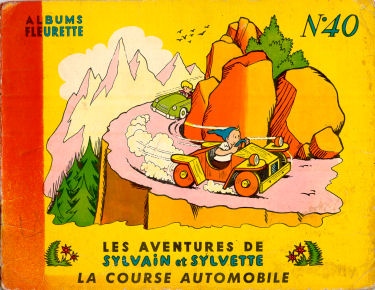
\includegraphics[width=.6\textwidth]{Sylvain+Sylvette_Course.jpg}} 
\newpage           

\item \underline{Résolution du système : }\\

\begin{tabular}{lp{3.5cm}ll}
\multicolumn{4}{l}{
$\begin{cases}
\qquad\dfrac{88}{V_1} -\dfrac{42}{V_2} \!\!\!\!\!\!\!\! &= 1 \\
& \\
\dfrac{106}{V_1} x -\dfrac{24}{V_2} y \!\!\!\!\!\!\!\!&= 1,5  \\
\end{cases}$} \\
& & & \\
\multicolumn{4}{l}{
Le système est linéaire si l'on pose :
       $X=\dfrac{1}{V_1} \text{ et }  Y=\dfrac{1}{V_2}$}\\
& & & \\
\begin{minipage}{4cm}
$\begin{cases}
 \; \; \; 88X - 42Y \!\!\!\!\!\!\!\!&= 1 \\
106X - 24Y\!\!\!\!\!\!\!\! &= 1,5  \\
\end{cases}$ \\
\end{minipage}  &  \multicolumn{1}{|l}{$\begin{array}{l}
                     24\\ -42 \\ 
                  \end{array}$ } & 
                   \begin{minipage}{4cm}       
                         $\begin{cases}
                             \; \; \; 88X - 42Y \!\!\!\!\!\!\!\!&= 1 \\
                            106X - 24Y \!\!\!\!\!\!\!\!&= 1,5  \\
                          \end{cases}$ 
                \end{minipage} &  \multicolumn{1}{|l}{ $\begin{array}{l}
                                        106\\-88\\ 
                                  \end{array}$}\\
& & & \\   
\begin{minipage}{4cm}
$\begin{cases}
 \quad 2112X - 1008Y \!\!\!\!\!\!\!\!&= 24 \\
-4452X - 1008Y \!\!\!\!\!\!\!\!&= -63  \\
\end{cases}$ \\
\end{minipage}  &  & 
                   \begin{minipage}{4cm}       
                         $\begin{cases}
                             \quad 9328X - 4452Y \!\!\!\!\!\!\!\!&= 106 \\
                            -9328X + 2112Y \!\!\!\!\!\!\!\!&= -132  \\
                          \end{cases}$ 
                \end{minipage} &  \\
& & & \\                           
\cline{1-1} \cline{3-3}
\multicolumn{1}{l}{$\qquad \qquad \; \; \; -2340X = -39$} &&
               \multicolumn{1}{l}{$\qquad \qquad \; \; \; -2340Y =-26$}&\\
$\qquad \qquad \qquad \quad \;\; \; X = \dfrac{1}{60}$ && $\qquad \qquad \qquad \quad \;  \; \; Y = \dfrac{1}{90}$& \\
\end{tabular}\\

Il vient : $\dfrac{1}{V_1} = \dfrac{1}{60} $ 
       et  $\dfrac{1}{V_2} = \dfrac{1}{90} $\\


\item \underline{Réponse au problème } :\\

Sylvain roule à 60km/h et les 2 Sylvettes à 90km/h.
  
\end{enumerate} 

\ifdefined\COMPLETE
\else
    \end{document}
\fi  \newpage $\;$ \newpage

\section{Trigonométrie}
\subsection{Cercle trigonométrique}
On appelle cercle trigonométrique tout cercle de rayon $R=1$ sur lequel on a choisi une origine $I$ et un sens de parcours appelé « sens trigonométrique ». 

%------------- Cerlcle trigonométrique ------------------

\hspace*{2cm}
\begin{tikzpicture}[line cap=round,line join=round,>=triangle 45,x=1.0cm,y=1.0cm,scale=.8]
\clip(-3,-3) rectangle (3,3);
\draw [color=gray] (0,0) circle (2cm);
\draw (0,0)-- (2,0);
\draw [shift={(0,0)}] plot[domain=0.17:1.12,variable=\t]({1*2.35*cos(\t r)+0*2.35*sin(\t r)},{0*2.35*cos(\t r)+1*2.35*sin(\t r)});
\draw [->] (1.05,2.1) -- (1.03,2.11);
\fill (0,0) circle (1.5pt);
\draw (0,0) node [below]{$O$};
\fill (2,0) circle (1.5pt);
\draw(2,0) node [right] {$I$};
% \draw (-1/2, sqrt(3)/2) node [left] {$I'$};
\end{tikzpicture}\raisebox{10ex}{$R=OI=1$}
 
\subsection{Image d'un nombre réel sur le cercle trigonométrique}

Soit $\mathcal{C}$ un cercle trigonométrique.

$\mathcal{P} = 2{\pi}R = 2\pi \text{ puisque } R=1$ \\ 

\begin{itemize}
\item [\ding{87}] À tout nombre réel $x$ correspond un point et un seul de $\mathcal{C}$ appelé « image de $x$ sur $\mathcal{C}$ 
noté $M(x)$.\\

$M(\pi) = I'$ 
\item [\ding{87}] Tout point $M$ de  $\mathcal{C}$ est l'image d'une infinité de nombres réels.

\begin{minipage}{9cm}
\begin{tabbing}
Si \= $M$ est $\qquad\quad$ \= l'image de $x$ sur  $\mathcal{C}$\\
   \>  $M$ est aussi \> l'image de $x+2\pi$ \\
   \>  $M$ est aussi \> l'image de $x+4\pi$ \\  
   \>  $M$ est aussi \> l'image de $x+6\pi$\ldots  \\   
   \>  $M$ est aussi \> l'image de $x+2k\pi \quad k\in \mathbb{Z}$ \\    
\end{tabbing}
\hspace*{5cm}
\end{minipage}
%
%------- Enroulement des réels sur le cercle trigo --------
% Pour tracer les courbes de Bésier : 
% ajouter, 
% 1 - dans les préférences de TexMaker, 
%     dans  la ligne  pdflatex 
%     "--shell-escape  -enable-write18 " avant "%.tex"
% 2 - un lien vers gnuplot dans le répertoire  texbin 
%     cd /usr/texbin/
%     sudo ln -s /opt/local/bin/gnuplot ./gnuplot
%
\raisebox{-30ex}{\begin{tikzpicture}[line cap=round,line join=round,>=triangle 45,x=1.0cm,y=1.0cm, scale=.55]
\draw[->,color=black] (0,-7.1) -- (0,11.85);
\foreach \y in {-6,-4,-2,2,4,6,8,10}
\draw[shift={(0,\y)},color=black] (2pt,0pt) -- (-2pt,0pt);
\clip(-4.19,-7.1) rectangle (3.6,11.85);
\draw(-1,0) circle (1cm);
\draw (-2,0)-- (0,0);
\draw [shift={(1.63,-0.1)}] plot[domain=2.04:3.11,variable=\t]({1*3.63*cos(\t r)+0*3.63*sin(\t r)},{0*3.63*cos(\t r)+1*3.63*sin(\t r)});
\draw[smooth,samples=100,domain=0.0:1.0] plot[parametric] function{(1-t)**3*0.01+3*(1-t)**2*t*(-2.81)+3*(1-t)*t**2*(-2.81)+t**3*(-1),(1-t)**3*4.72+3*(1-t)**2*t*2.77+3*(1-t)*t**2*(-1.53)+t**3*(-1)};
\draw[smooth,samples=100,domain=0.0:1.0] plot[parametric] function{(1-t)**3*0+3*(1-t)**2*t*(-7)+3*(1-t)*t**2*2.23+t**3*0,(1-t)**3*6.28+3*(1-t)**2*t*(-2)+3*(1-t)*t**2*(-4.14)+t**3*0};
\draw [shift={(-0.13,-0.64)}] plot[domain=3.54:4.85,variable=\t]({1*0.94*cos(\t r)+0*0.94*sin(\t r)},{0*0.94*cos(\t r)+1*0.94*sin(\t r)});
\draw [shift={(1.64,5.56)}] plot[domain=1.97:2.71,variable=\t]({1*4.2*cos(\t r)+0*4.2*sin(\t r)},{0*4.2*cos(\t r)+1*4.2*sin(\t r)});
\draw [shift={(0.64,7.45)}] plot[domain=1.75:2.8,variable=\t]({1*3.6*cos(\t r)+0*3.6*sin(\t r)},{0*3.6*cos(\t r)+1*3.6*sin(\t r)});
\draw[smooth,samples=100,domain=0.0:1.0] plot[parametric] function{(1-t)**3*0+3*(1-t)**2*t*(-9.62)+3*(1-t)*t**2*7.32+t**3*(-1),(1-t)**3*7.85+3*(1-t)**2*t*(-8.49)+3*(1-t)*t**2*(-1.24)+t**3*1};
\draw [shift={(0.02,0.37)}] plot[domain=1.59:2.59,variable=\t]({1*1.2*cos(\t r)+0*1.2*sin(\t r)},{0*1.2*cos(\t r)+1*1.2*sin(\t r)});
\draw [shift={(-1.27,-0.26)}] plot[domain=4.29:5.13,variable=\t]({1*3.15*cos(\t r)+0*3.15*sin(\t r)},{0*3.15*cos(\t r)+1*3.15*sin(\t r)});
\draw [shift={(-0.52,-0.36)}] plot[domain=4.13:4.83,variable=\t]({1*4.39*cos(\t r)+0*4.39*sin(\t r)},{0*4.39*cos(\t r)+1*4.39*sin(\t r)});
\draw [shift={(0.18,-1.34)}] plot[domain=3.85:4.68,variable=\t]({1*4.95*cos(\t r)+0*4.95*sin(\t r)},{0*4.95*cos(\t r)+1*4.95*sin(\t r)});
\draw (-1,-1) -- (-1,1) ; 
\draw [->] (-2.73,8.71) -- (-2.75,8.66);
\draw [->] (-2.12,7.42) -- (-2.17,7.31);
\draw [->] (-2.4,-3.2) -- (-2.56,-3.14);
\draw [->] (-2.85,-4.07) -- (-2.92,-4.02);
\draw [->] (-3.51,-4.64) -- (-3.57,-4.57);
\draw [->] (.01,-.02) -- (0,0);
\draw [->] (-0.99,1.01) -- (-1,1);
\draw [->] (-0.98,.995) -- (-1,1);
\draw [->] (-0.99,-1.02) -- (-1,-1);
\draw [->] (-1.01,-1) -- (-1,-1);
\draw [->] (-2,.01) -- (-2,0);
\fill  (0,1.57) circle (1.5pt);
\draw (0,1.57) node [right] {${\pi}/2$};
\fill  (0,3.14) circle (1.5pt);
\draw (0,3.14) node [right]{$\pi$};
\fill  (0,9.42) circle (1.5pt);
\draw (0,9.42) node [right]{$3\pi$};
\fill  (0,11) circle (1.5pt);
\draw (0,11) node [right]{$\dfrac{7\pi}{2}$};
\fill  (0,-3.14) circle (1.5pt);
\draw (0,-3.14) node [right]{$-\pi$};
\fill  (0,-4.71) circle (1.5pt);
\draw (0,-4.71) node [right]{$-\dfrac{3\pi}{2}$};
\fill  (0,-1.57) circle (1.5pt);
\draw (0,-1.57) node [right]{$-\dfrac{\pi}{2}$};
\fill  (0,-6.28) circle (1.5pt);
\draw (0,-6.28) node [right]{$-2\pi$};
\fill  (-1,0) circle (1.5pt);
\draw (-1.28,-0.16) node {$O$};
\fill  (0,4.72) circle (1.5pt);
\draw (0,4.72) node [right]{$\dfrac{3\pi}{2}$};
\fill  (-1,-1) circle (1.5pt);
\draw (-1.1,-1) node [below] {$J'$};
\fill  (0,6.28) circle (1.5pt);
\draw (0,6.28) node [right]{$2\pi$};
\fill  (0,0) circle (1.5pt);
\draw (0,0) node [right]{$I$};
\fill  (-2,0) circle (1.5pt);
\draw (-1.7,0.27) node {$I'$};
\fill  (0,7.85) circle (1.5pt);
\draw (0,7.85) node [right]{$\dfrac{5\pi}{2}$};
\fill  (-1,1) circle (1.5pt);
\draw (-0.87,1.28) node {$J$};
\end{tikzpicture}}

\end{itemize}
\newpage

% ---------- Points remarquable du cercle trigo -----------

\begin{tikzpicture}[line cap=round,line join=round,>=triangle 45,x=1.0cm,y=1.0cm, scale=4]
\clip(-1.4,-1.4) rectangle (1.5,1.2);
\draw(0,0) circle (1cm);
\draw [dash pattern=on 1pt off 1pt,color=gray] (-1,1)-- (-1,-1);
\draw [dash pattern=on 1pt off 1pt,color=gray] (-1,-1)-- (1,-1);
\draw [dash pattern=on 1pt off 1pt,color=gray] (1,-1)-- (1,1);
\draw [dash pattern=on 1pt off 1pt,color=gray] (1,1)-- (-1,1);
\draw (-1,1)-- (1,-1);
\draw (1,1)-- (-1,-1);
\draw (0,1) node[above left] {$J$};
\draw [line width=1.2pt] (0,1)-- (0,-1);
\draw [color=violet](1,0) node[above right] {$M(0)$};
\draw [color=violet](1,0) node[below right] {$M(2\pi)\ldots$};
\draw [color=violet](-1,0) node[below left] {$ M(\pi) $};
\draw [dash pattern=on 1pt off 1pt,color=gray] (-0.5,0.87)-- (0.5,0.87);
\draw [dash pattern=on 1pt off 1pt,color=gray] (0.5,0.87)-- (0.5,-0.87);
\draw [dash pattern=on 1pt off 1pt,color=gray] (0.5,-0.87)-- (-0.5,-0.87);
\draw [dash pattern=on 1pt off 1pt,color=gray] (-0.5,-0.87)-- (-0.5,0.87);
\draw [dash pattern=on 1pt off 1pt,color=gray] (-0.87,0.5)-- (0.87,0.5);
\draw [dash pattern=on 1pt off 1pt,color=gray] (0.87,0.5)-- (0.87,-0.5);
\draw [dash pattern=on 1pt off 1pt,color=gray] (0.87,-0.5)-- (-0.87,-0.5);
\draw [dash pattern=on 1pt off 1pt,color=gray] (-0.87,-0.5)-- (-0.87,0.5);
\draw [line width=1.2pt] (-1,0)-- (1,0);
\begin{scriptsize}
\fill  (0,0) circle (.5pt);
\draw (0,0) node [below left]{$O$};
\fill [color=blue] (0.71,0.71) circle (.5pt);
\draw[color=blue] (0.71,0.71) node[right] {$M(\dfrac{\pi}{4})$};
\fill [color=blue] (-0.71,0.71) circle (.5pt);
\draw[color=blue] (-0.71,0.71) node [left]{$M(\dfrac{3\pi}{4})$};
\fill [color=VertClair] (0.87,0.5) circle (.5pt);
\draw[color=VertClair] (0.87,0.5) node [right] {$M(\dfrac{\pi}{6})$};
\fill [color=darkgreen] (0.5,0.87) circle (.5pt);
\draw[color=darkgreen] (0.5,0.87) node [right]{$M(\dfrac{\pi}{3})$};
\fill [color=violet] (0,1) circle (.5pt);
\draw[color=violet] (0,1) node [above right]{$M(\dfrac{\pi}{2})$};
\fill [color=darkgreen] (-0.5,0.87) circle (.5pt);
\draw[color=darkgreen] (-0.5,0.87) node [left]{$M(\dfrac{2\pi}{3)})$};
\fill [color=VertClair] (-0.87,0.5) circle (.5pt);
\draw[color=VertClair] (-0.87,0.5) node [left]{$M(\dfrac{5\pi}{6})$};
\fill [color=blue] (-1,0) circle (.5pt);
\draw[color=blue] (-1,0) node [above left]{$I'$};
\fill [color=blue] (1,0) circle (.5pt);
\draw[color=blue] (1,0) node [above left]{$I$};
\fill [color=blue] (0,-1) circle (.5pt);
\draw[color=blue] (0,-1) node[below left] {$J'$};
\fill [color=VertClair] (-0.87,-0.5) circle (.5pt);
\draw[color=VertClair] (-.87,-0.5) node[left]{$M(\dfrac{7\pi}{6})$};
\fill [color=blue] (-0.71,-0.71) circle (.5pt);
\draw[color=blue] (-0.71,-0.71) node [left]{$M(\dfrac{5\pi}{4})$};
\fill [color=darkgreen] (-0.5,-0.87) circle (.5pt);
\draw[color=darkgreen] (-0.5,-0.87) node [left]{$M(\dfrac{4\pi}{3})$};
\fill [color=violet] (0,-1) circle (.5pt);
\draw[color=violet] (0,-1) node [below right]{$M(\dfrac{3\pi}{2})$};
\fill [color=darkgreen] (0.5,-0.87) circle (.5pt);
\draw[color=darkgreen] (0.5,-0.87) node [right] {$(\dfrac{5\pi}{3})$};
\fill [color=blue] (0.71,-0.71) circle (.5pt);
\draw[color=blue] (0.71,-0.71) node [right] {$M(\dfrac{7\pi}{4})$};
\fill [color=VertClair] (0.87,-0.5) circle (.5pt);
\draw[color=VertClair](0.87,-0.5)node[right]{$M(\dfrac{11\pi}{6})$};
\end{scriptsize}
\end{tikzpicture}\\

Notion de congruence 

$\dfrac{5\pi}{2} \equiv \dfrac{\pi}{2} \left[2\pi\right] \text{ car } \dfrac{5\pi}{2}-\dfrac{\pi}{2} = 2\pi \longleftarrow \text{ Un tour de cercle.}$\\

$\dfrac{9\pi}{2} \equiv \dfrac{\pi}{2} \left[2\pi\right] \text{ car } \dfrac{9\pi}{2}-\dfrac{\pi}{2} = 4\pi \longleftarrow \text{ Deux tours de cercle.}$\\

$\dfrac{15\pi}{2} \cancel{\equiv} \dfrac{\pi}{2} \left[2\pi\right] \text{ car } \dfrac{15\pi}{2}-\dfrac{\pi}{2} = 7\pi \longleftarrow \dfrac{7}{2}\text{ tours de cercle.}$\\

Exercice : Placer sur un cercle trigonométrique les images de : \\
$\dfrac{223\pi}{6},\quad  \dfrac{252\pi}{4}, \quad \dfrac{431\pi}{3},\quad  \dfrac{1035\pi}{4}, \quad \dfrac{1702\pi}{3}, \quad \dfrac{2015\pi}{6}$ \\

\bigskip 

\begin{tabular}{c@{}c@{}c@{}c@{}c@{}l}
\ding{43} 
   $\qquad\dfrac{223\pi}{6}  $ & 
        $ \equiv \dfrac{7\pi}{6}   $ &
           $ \left[2\pi\right] $ & 
               $\text{ car } \dfrac{223\pi}{6}-\dfrac{7\pi}{6}  $ & 
                  $ = 36\pi   $ &
                    $ \longleftarrow \text{ 18 tours de cercle.}$\\
&&&\\
\ding{43}$\qquad\dfrac{291\pi}{4}   $ & $ \equiv \dfrac{3\pi}{4}   $ & $ \left[2\pi\right] $ & $\text{ car } \dfrac{291\pi}{4}-\dfrac{3\pi}{4}  $ & $ = 72\pi   $ & $ \longleftarrow \text{ 36 tours de cercle.}$\\
&&&\\
\ding{43}$\qquad\dfrac{431\pi}{3}   $ & $ \equiv \dfrac{5\pi}{3}   $ & $ \left[2\pi\right] $ & $\text{ car } \dfrac{231\pi}{3}-\dfrac{5\pi}{3}  $ & $ = 142\pi   $ & $ \longleftarrow \text{ 71 tours de cercle.}$\\
&&&\\
\ding{43}$\qquad\dfrac{1035\pi}{4}   $ & $ \equiv \dfrac{3\pi}{4}   $ & $ \left[2\pi\right] $ & $\text{ car } \dfrac{1035\pi}{4}-\dfrac{3\pi}{4}  $ & $ = 258\pi   $ & $ \longleftarrow \text{ 129 tours de cercle.}$\\
&&&\\
\ding{43}$\qquad\dfrac{1702\pi}{3}   $ & $ \equiv \dfrac{4\pi}{3}   $ & $ \left[2\pi\right] $ & $\text{ car } \dfrac{1702\pi}{3}-\dfrac{4\pi}{3}  $ & $ = 566\pi   $ & $ \longleftarrow \text{ 283 tours de cercle.}$\\
&&&\\
\ding{43}$\qquad\dfrac{2015\pi}{6}   $ & $ \equiv \dfrac{11\pi}{6}   $ & $ \left[2\pi\right] $ & $\text{ car } \dfrac{2015\pi}{6}-\dfrac{11\pi}{6}  $ & $ = 334\pi   $ & $ \longleftarrow \text{ 167 tours de cercle.}$\\
\end{tabular}

\newpage

\subsection{Cosinus et sinus d'un nombre réel}

Soit $\mathcal{C}$ un cercle trigonométrique.\\
Soit $M(x)$ l'image de $x$ sur $\mathcal{C}$.\\
Soit $H$ le projeté orthogonal de $M$ sur $(OI)$.\\
Soit $K$ le projeté orthogonal de $M$ sur $(OJ)$.\\

% ------•---- Projetés des points du cercle trigo -----------


\begin{tikzpicture}[line cap=round,line join=round,>=triangle 45,x=1.0cm,y=1.0cm,scale=.8]
\clip(0.3,1) rectangle (14,12.56);
\draw[line width=0.4pt,color=red] (3,11.44) -- (3.21,11.44) -- (3.21,11.65) -- (3,11.65) -- cycle; 
\draw[line width=0.4pt,color=red] (4.13,10.21) -- (3.92,10.21) -- (3.92,10) -- (4.13,10) -- cycle; 
\draw[line width=0.4pt,color=red] (9.79,11) -- (9.79,10.79) -- (10,10.79) -- (10,11) -- cycle; 
\draw[line width=0.4pt,color=red] (8.48,10) -- (8.48,10.21) -- (8.27,10.21) -- (8.27,10) -- cycle; 
\draw[line width=0.4pt,color=red] (1.99,3.79) -- (2.2,3.79) -- (2.2,4) -- (1.99,4) -- cycle; 
\draw[line width=0.4pt,color=red] (3,2.49) -- (2.79,2.49) -- (2.79,2.27) -- (3,2.27) -- cycle; 
\draw[line width=0.4pt,color=red] (11.51,4) -- (11.51,3.79) -- (11.72,3.79) -- (11.72,4) -- cycle; 
\draw[line width=0.4pt,color=red] (10.21,2.98) -- (10.21,3.19) -- (10,3.19) -- (10,2.98) -- cycle; 
\draw(3,4) circle (2cm);
\draw(10,4) circle (2cm);
\draw(3,10) circle (2cm);
\draw(10,10) circle (2cm);
\draw (1,10)-- (5,10);
\draw (3,12)-- (3,8);
\draw [dash pattern=on 5pt off 5pt,color=red] (4.13,11.65)-- (3,11.65);
\draw [dash pattern=on 5pt off 5pt,color=red] (4.13,11.65)-- (4.13,10);
\draw (4.6,8.66) node[anchor=north west] {\parbox{2.12 cm}{${\color{blue}\cos x=OH}\\{\color{Green}\sin x = OK}$}};
\draw [line width=1.6pt,very thick,color=Green] (3,11.65)-- (3,10);
\draw [line width=1.6pt,very thick,color=blue] (3,10)-- (4.13,10);
\draw (10,12)-- (10,8);
\draw [dash pattern=on 5pt off 5pt,color=red] (8.27,10)-- (8.27,11);
\draw (12,10)-- (8,10);
\draw [dash pattern=on 5pt off 5pt,color=red] (8.27,11)-- (10,11);
\draw (10,6)-- (10,2);
\draw (8,4)-- (12,4);
\draw [dash pattern=on 5pt off 5pt,color=red] (11.72,4)-- (11.72,2.98);
\draw [dash pattern=on 5pt off 5pt,color=red] (11.72,2.98)-- (10,2.98);
\draw (1,4)-- (5,4);
\draw (3,6)-- (3,2);
\draw [dash pattern=on 5pt off 5pt,color=red] (3,2.27)-- (1.99,2.27);
\draw [dash pattern=on 5pt off 5pt,color=red] (1.99,2.27)-- (1.99,4);
\draw (0,0.24) node[anchor=north west] {\parbox{2.12 cm}{${\color{blue}\cos x=OH}\\{\color{Green}\sin x = OK}$}};
\draw (11.68,8.68) node[anchor=north west] {\parbox{2.2 cm}{${\color{blue}\cos x=-OH}\\{\color{Green}\sin x = OK}$}};
\draw (4.62,2.7) node[anchor=north west] {\parbox{2.2 cm}{${\color{blue}\cos x= -OH}\\{\color{Green}\sin x = -OK}$}};
\draw (11.62,2.6) node[anchor=north west] {\parbox{2.16 cm}{${\color{blue}\cos x=OH}\\{\color{Green}\sin x = -OK}$}};
\draw [very thick, color=blue] (8.27,10)-- (10,10);
\draw [very thick,color=Green] (10,10)-- (10,11);
\draw [very thick, color=blue] (3,4)-- (1.99,4);
\draw [very thick,color=Green] (3,4)-- (3,2.27);
\draw [very thick, color=blue] (10,4)-- (11.72,4);
\draw [very thick,color=Green] (10,4)-- (10,2.98);

\fill (3,4) circle (1.5pt);
\draw(3,4) node [below left]{$O$};
\fill (10,4) circle (1.5pt);
\draw(10,4) node [below left]{$O$};
\fill (3,10) circle (1.5pt);
\draw(3,10) node [below left]{$O$};
\fill (10,10) circle (1.5pt);
\draw(10,10) node [below left]{$O$};
\fill (1,10) circle (1.5pt);
\draw(1,10) node [left] {$I'$};
\fill (5,10) circle (1.5pt);
\draw(5.32,10.1) node {$I$};
\fill (3,12) circle (1.5pt);
\draw(3,12) node [above]{$J$};
\fill (3,8) circle (1.5pt);
\draw(3,8) node [below] {$J'$};
\fill [color=red] (4.13,11.65) circle (1.5pt);
\draw[color=red] (4.13,11.65) node [right] {$M(x)$};
\fill [color=red] (3,11.65) circle (1.5pt);
\draw[color=red] (3,11.65) node [left] {$K$};
\fill [color=red] (4.13,10) circle (1.5pt);
\draw[color=red] (4.13,10) node [below] {$H$};
\fill [color=red] (8.27,11) circle (1.5pt);
\draw[color=red] (8.27,11) node [left]{$M(x)$};
\fill [color=red] (1.99,2.27) circle (1.5pt);
\draw[color=red] (1.99,2.27) node [left]{$M(x)$};
\fill [color=red] (11.72,2.98) circle (1.5pt);
\draw[color=red] (11.72,2.98) node [right]{$M(x)$};
\fill [color=red] (10,11) circle (1.5pt);
\draw[color=red] (10,11) node [right]{$K$};
\fill [color=red] (8.27,10) circle (1.5pt);
\draw[color=red] (8.27,10) node [below]{$H$};
\fill [color=red] (10,2.98) circle (1.5pt);
\draw[color=red] (10,2.98) node [left]{$K$};
\fill [color=red] (11.72,4) circle (1.5pt);
\draw[color=red] (11.72,4) node [above]{$H$};
\fill [color=red] (3,2.27) circle (1.5pt);
\draw[color=red] (3,2.27) node [right]{$K$};
\fill [color=red] (1.99,4) circle (1.5pt);
\draw[color=red] (1.99,4) node [above]{$H$};
\fill (8,10) circle (1.5pt);
\draw(8,10)  node [left] {$I'$};
\fill (12,10) circle (1.5pt);
\draw(12,10) node [right] {$I$};
\fill (1,4) circle (1.5pt);
\draw(1,4)  node [left] {$I'$};
\fill (5,4) circle (1.5pt);
\draw(5,4) node [right] {$I$};
\fill (8,4) circle (1.5pt);
\draw(8,4)  node [left] {$I'$};
\fill (12,4) circle (1.5pt);
\draw(12,4) node [right] {$I$};
\fill (10,12) circle (1.5pt);
\draw(10,12) node [above] {$J$};
\fill (10,8) circle (1.5pt);
\draw(10,8) node [below] {$J'$};
\fill (10,6) circle (1.5pt);
\draw(10,6)  node [above] {$J$};
\fill (10,2) circle (1.5pt);
\draw(10,2) node [below] {$J'$};
\fill (3,6) circle (1.5pt);
\draw(3,6)  node [above] {$J$};
\fill (3,2) circle (1.5pt);
\draw(3,2) node [below] {$J'$};

\end{tikzpicture}


% ------•---- Les quatres cadrans --------------------------

Quatre quadrants.

\parbox{5cm}{\begin{tikzpicture}[line cap=round,line join=round,>=triangle 45,x=1.0cm,y=1.0cm, scale=.8]
\clip (0.38,7.29) rectangle (6.04,12.92);
\draw (3,10) circle (2cm);
\draw (1,10)-- (5,10);
\draw (3,12)-- (3,8);
\draw (3.75,10.75)    node {\Huge \ding{172}};
\draw (2.25,10.75)       node {\Huge  \ding{173}};
\draw (2.25,9)     node {\Huge  \ding{174}};
\draw (3.75,9)  node {\Huge  \ding{175}};
\fill (3,10) circle (1.5pt);
\draw (3,10) node [below left]{$O$};
\fill (1,10) circle (1.5pt);
\draw (1,10) node [left] {$I'$};
\fill (5,10) circle (1.5pt);
\draw (5,10) node [right] {$I$};
\fill (3,12) circle (1.5pt);
\draw (3,12) node [above]{$J$};
\fill (3,8) circle (1.5pt);
\draw (3,8) node [below]{$J'$};
\end{tikzpicture}}
\parbox{10cm}{
   \ding{172} $\longrightarrow$\raisebox{-1ex}{$ \begin{array}{c}  
\cos (x) > 0 \\ 
\sin (x) >0 \\ 
   \end{array} 
        \qquad$}  
 \ding{173}
        $\longrightarrow$\raisebox{-1ex}{$\begin{array}{c}  
                 \cos (x) < 0 \\ 
                 \sin (x) > 0 \\ 
               \end{array}$}\\
               
               
\ding{174} 
    $\longrightarrow$\raisebox{-1ex}{$ \begin{array}{c}  
\cos (x) < 0 \\ 
\sin (x) < 0 \\ 
   \end{array} 
        \qquad$}  \ding{175}$\longrightarrow$\raisebox{-1ex}{ $\begin{array}{c}  
                 \cos (x) > 0 \\ 
                 \sin (x) < 0 \\ 
               \end{array}$}\\               
} \\
\renewcommand{\arraystretch }{1.75}
En particulier : 
\begin{quote}
{
\begin{tabular}{l@{$\;$}c@{$\qquad$}l@{$\;$}c}
$\bullet$  & $\cos 0 = 1 $ 
         & $\bullet$ & $\cos \dfrac{\pi}{2} = 0 $ \\  
          & $\sin 0 = 0 $ 
         &  & $\sin \dfrac{\pi}{2} = 1 $ \\  
& & & \\
$\bullet$  & $\cos \pi = -1 $ 
         & $\bullet$ & $\cos \dfrac{3\pi}{2} = 0 $ \\  
  & $\sin \pi = 0 $ 
         & & $\sin \dfrac{3\pi}{2} = -1 $ \\                             
\end{tabular}              
}
\end{quote}
\renewcommand{\arraystretch }{1}
\newpage 

Propriétés fondamentales pour $k \in \mathbb{Z}$  

\begin{quote}
\begin{tabular}{l@{$\,$}cc@{$\,$}l}
\ding{81} & Pour tout $x\in \Re$ & $\bullet$ & $-1
                       \leqslant \cos x  \leqslant 1 $ \\
          &          & $\bullet$ & $-1
                       \leqslant \sin x  \leqslant 1 $ \\
 & & & \\ 
 \ding{81} & Pour tout $x\in \Re$ & $\bullet$ 
                     & $ \cos (x+2k\pi) = \cos x $ \\
       &   & $\bullet$ & $ \sin x  (x+2k\pi) = \sin x $ \\
                        & & & \\ 
 \ding{81} & Pour tout $x\in \Re$ & $\bullet$ 
         & $ \cos^2 (x+2k\pi) + \sin^2 (x+2k\pi) = 1 $ \\

\end{tabular}\\

\bigskip

$(O, \overrightarrow{OI},  \overrightarrow{OJ})$ un repère orthonormal.\\

$M(\cos x, \sin x)$ dans $(O, \overrightarrow{OI},  \overrightarrow{OJ})$. \\

\begin{tabular}{r@{\,}l}
$ \cos^2 (x+2k\pi) + \sin^2 x $ &$= OH^2 + OK^2$\\
 &$= OH^2 + HM^2 $\\
 &$= OM^2$\\
 &$= 1 \qquad \qquad \text{ car }\; OM = 1 $\\ 
\end{tabular}\\

{\renewcommand{\arraystretch }{1.75}
\begin{tabular}{ll}
 
\begin{tikzpicture}[line cap=round,line join=round,>=triangle 45,x=1.0cm,y=1.0cm,scale=1]
\clip(-2.25,-2.38) rectangle (2.37,2.39);
\draw[line width=0.4pt] (0,1.32) -- (0.1,1.32) -- (0.1,1.42) -- (0,1.42) -- cycle; 
\draw[line width=0.4pt] (1.41,0.1) -- (1.31,0.1) -- (1.31,0) -- (1.41,0) -- cycle; 
\draw(0,0) circle (2cm);
\draw (-2,0)-- (2,0);
\draw (0,2)-- (0,-2);
\draw [dash pattern=on 2pt off 2pt] (1.41,1.42)-- (0,1.42);
\draw [dash pattern=on 2pt off 2pt] (1.41,1.42)-- (1.41,0);
\draw [line width=1.6pt] (0,1.42)-- (0,0);
\draw [line width=1.6pt] (0,0)-- (1.41,0);
\draw [line width=0.4pt] (0,2)-- (0,0);
\draw [line width=0.4pt] (0,0)-- (2,0);
\draw [line width=0.4pt] (2,0)-- (2,2);
\draw [line width=0.4pt] (2,2)-- (0,2);
\draw (0,0)-- (2,2);

\fill  (0,0) circle (1.5pt);
\draw(0,0) node [below left] {$O$};
\fill (-2,0) circle (1.5pt);
\draw(-2,0) node [left] {$I'$};
\fill (2,0) circle (1.5pt);
\draw(2,0) node [right] {$I$};
\fill (0,2) circle (1.5pt);
\draw(0,2) node [above] {$J$};
\fill (0,-2) circle (1.5pt);
\draw(0,-2) node [below] {$J'$};
\fill (1.41,1.42) circle (1.5pt);
\draw(1.41,1.42) node [above] {$M$};
\fill (0,1.42) circle (1.5pt);
\draw(0,1.42) node [left]{$K$};
\fill (1.41,0) circle (1.5pt);
\draw(1.41,0) node [below] {$H$};

\end{tikzpicture}


         &  \raisebox{27ex}{ \ding{81}}
            \raisebox{16.5ex}{              
         \parbox{.5\textwidth}{ 
        Cosinus et sinus de $\dfrac{\pi}{4}$ \\
        
        $ \begin{array}{r@{\;}l}
                 \cos^2 x + \sin^2 x              &= 1 \\
\cos^2 (\dfrac{\pi}{4}) + \sin^2 (\dfrac{\pi}{4}) &= 1 \\
                             2 sin^2 \dfrac{\pi}{4}      &= 1 \\ 
                         cos^2    \dfrac{\pi}{4} =     sin^2  \dfrac{\pi}{4} &= 
   \dfrac{1}{2} \quad \text { donc }= \dfrac{\sqrt{2}}{2} \text { ou } \cancel {-\dfrac{\sqrt{2}}{2}}\\  
        \end{array}$
         }}\\
\end{tabular}\\
\vspace*{-1cm}
\begin{center}
\fcolorbox{black}  {white}{
\hbox{
$\cos \dfrac{\pi}{4} = \dfrac{\sqrt{2}}{2} \quad \text{ et } \quad \sin \dfrac{\pi}{4} =  \dfrac{\sqrt{2}}{2} $ 
}}
\end{center}

\bigskip 

\begin{tabular}{ll}
 
% \definecolor{uuuuuu}{rgb}{0.27,0.27,0.27}
% \definecolor{qqffqq}{rgb}{0,1,0}
% \definecolor{ffqqqq}{rgb}{1,0,0}
% \definecolor{qqqqff}{rgb}{0,0,1}
\begin{tikzpicture}[line cap=round,line join=round,>=triangle 45,x=1.0cm,y=1.0cm,scale=1]
\clip(-2.25,-2.38) rectangle (2.37,2.39);
\draw[line width=0.4pt] (0,1.64) -- (0.1,1.64) -- (0.1,1.73) -- (0,1.73) -- cycle; 
\draw[line width=0.4pt] (1,0.1) -- (0.9,0.1) -- (0.9,0) -- (1,0) -- cycle; 
\draw(0,0) circle (2cm);
\draw (-2,0)-- (2,0);
\draw (0,2)-- (0,-2);
\draw [dash pattern=on 2pt off 2pt] (1,1.73)-- (0,1.73);
\draw [dash pattern=on 2pt off 2pt] (1,1.73)-- (1,0);
\draw [line width=1.6pt] (0,1.73)-- (0,0);
\draw [line width=1.6pt] (0,0)-- (1,0);
\draw  (0,0)-- (2,0);
\draw  (2,0)-- (1,1.73);
\draw  (1,1.73)-- (0,0);

\fill  (0,0) circle (1.5pt);
\draw(0,0) node [below left] {$O$};
\fill (-2,0) circle (1.5pt);
\draw(-2,0) node [left] {$I'$};
\fill (2,0) circle (1.5pt);
\draw(2,0) node [right] {$I$};
\fill (0,2) circle (1.5pt);
\draw(0,2) node [above] {$J$};
\fill (0,-2) circle (1.5pt);
\draw(0,-2) node [below] {$J'$};
\fill  (1,1.73) circle (1.5pt);
\draw (1.1,1.73) node [right]{$M$};
\fill  (0,1.73) circle (1.5pt);
\draw (0,1.73) node [left] {$K$};
\fill  (1,0) circle (1.5pt);
\draw (1,0) node [below] {$H$};
\end{tikzpicture}

         &  \raisebox{31ex}{ \ding{81}}
            \raisebox{10ex}{              
         \parbox{.5\textwidth}{ 
        Cosinus et sinus de $\dfrac{\pi}{3}$ \\
        
        $ \begin{array}{r@{\;}l}
                 \cos^2 x + \sin^2 x              &= 1 \\
\cos^2 (\dfrac{\pi}{3}) + \sin^2 (\dfrac{\pi}{3}) &= 1 \\
                                       & \qquad \qquad 0H=\dfrac{1}{2} \\
                     \dfrac{1}{4} + \sin^2 (\dfrac{\pi}{3})    &= 1 \\
                       \sin^2 (\dfrac{\pi}{3}) &= 1 - \dfrac{1}{4} \\
                          \sin^2 (\dfrac{\pi}{3}) -\dfrac{3}{4}  &= 0 \\ 
 \left( \sin (\dfrac{\pi}{3} - \sqrt{\dfrac{3}{4}}\right)  \left( \sin (\dfrac{\pi}{3}) +\sqrt{\dfrac{3}{4}}\right) &= 0 \\       
                                   \sin (\dfrac{\pi}{3}) &= 
\dfrac{\sqrt{3}}{2} \text { ou } \cancel {-\dfrac{\sqrt{3}}{2}}\\  
        \end{array}$
         }}\\         
\end{tabular}\\
}
\renewcommand{\arraystretch }{1}
\begin{center}
\fcolorbox{black}  {white}{
\hbox{
$\cos \dfrac{\pi}{3} = \dfrac{1}{2} \quad \text{ et } \quad \sin \dfrac{\pi}{3} =  \dfrac{\sqrt{3}}{2} $ 
}}
\end{center}

\newpage

{\renewcommand{\arraystretch }{1.75}
\begin{tabular}{ll}

\begin{tikzpicture}[line cap=round,line join=round,>=triangle 45,x=1.0cm,y=1.0cm]
\clip(-2.4,-2.38) rectangle (2.8,2.39);
\draw(0,0) circle (2cm);
\draw (-2,0)-- (2,0);
\draw (0,2)-- (0,-2);
\draw [dash pattern=on 2pt off 2pt] (1.73,1)-- (0,1);
\draw [dash pattern=on 2pt off 2pt] (1.73,1)-- (1.73,0);
\draw [line width=1.6pt] (0,1)-- (0,0);
\draw [line width=1.6pt] (0,0)-- (1.73,0);
\draw [line width=2pt](0,0)-- (1.73,1);
\draw [line width=2pt](1.73,1)-- (0,2);
\draw [line width=2pt](0,0)-- (0,2);
\draw (0,2)-- (0,0);
\fill  (0,0) circle (1.5pt);
\draw(0,0) node [below left] {$O$};
\fill (-2,0) circle (1.5pt);
\draw(-2,0) node [left] {$I'$};
\fill (2,0) circle (1.5pt);
\draw(2,0) node [right] {$I$};
\fill (0,2) circle (1.5pt);
\draw(0,2) node [above] {$J$};
\fill (0,-2) circle (1.5pt);
\draw(0,-2) node [below] {$J'$};
\fill  (1.73,1) circle (1.5pt);
\draw (1.73,1) node [right] {$M(\dfrac{\pi}{6})$};
\fill  (0,1) circle (1.5pt);
\draw (0,1) node [left]{$K$};
\fill  (1.73,0) circle (1.5pt);
\draw (1.73,0) node [below] {$H$};
\end{tikzpicture}
         &  \raisebox{31ex}{ \ding{81}}
            \raisebox{10ex}{              
         \parbox{.5\textwidth}{ 
        Cosinus et sinus de $\dfrac{\pi}{6}$ \\
        
        $ \begin{array}{r@{\;}l}
                 \cos^2 x + \sin^2 x              &= 1 \\
\cos^2 (\dfrac{\pi}{6}) + \sin^2 (\dfrac{\pi}{6}) &= 1 \\
                                       & \qquad \qquad OK=\dfrac{1}{2} \\
                      \cos^2 (\dfrac{\pi}{6})  +\dfrac{1}{4}   &= 1 \\
                       \cos^2 (\dfrac{\pi}{6}) &= 1 - \dfrac{1}{4} \\
                          \cos^2 (\dfrac{\pi}{6}) -\dfrac{3}{4}  &= 0 \\ 
 \left( \cos^2 (\dfrac{\pi}{6}) - \sqrt{\dfrac{3}{4}}\right)  \left( \cos^2 (\dfrac{\pi}{6})) +\sqrt{\dfrac{3}{4}}\right) &= 0 \\       
                                   \cos (\dfrac{\pi}{6}) &= 
\dfrac{\sqrt{3}}{2} \text { ou } \cancel {-\dfrac{\sqrt{3}}{2}}\\  
        \end{array}$
         }}\\         
\end{tabular}\\
}
\renewcommand{\arraystretch }{1}
\begin{center}
\fcolorbox{black}  {white}{
\hbox{
$\cos \dfrac{\pi}{6} = \dfrac{\sqrt{3}}{2} \quad \text{ et } \quad \sin \dfrac{\pi}{6} =  \dfrac{1}{2} $ 
}}
\end{center}
\end{quote}

\vspace{2cm}

\underline{Récapitulation} : \\

\bigskip 

\hspace*{2cm}
{\renewcommand{\arraystretch }{2.3}
\begin{tabular}{|c||c|c|c|c|c|}
\hline
$x$ & $0$ & $\dfrac{\pi}{6}$ & $\dfrac{\pi}{4}$ & $\dfrac{\pi}{3}$ & $\dfrac{\pi}{2}$ \\
\hline
\hline
$\cos x$ & $1$ & $\dfrac{\sqrt{3}}{2}$ & $\dfrac{\sqrt{2}}{2}$ & $\dfrac{1}{2}$ & $0$ \\
\hline
$\sin x$ & $0$ & $\dfrac{1}{2}$ & $\dfrac{\sqrt{2}}{2}$ & $\dfrac{\sqrt{3}}{2}$ & $1$ \\
\hline
\end{tabular}
}

\vspace{2cm}


\centerline{
 \renewcommand{\arraystretch }{2.3}
\begin{tabular}{|c||c|c|c|c|c|c|c|c|c|c|c|c|c|c|c|c|}
\hline
$x$ & $0$ & $\dfrac{\pi}{6}$ & $\dfrac{\pi}{4}$ & $\dfrac{\pi}{3}$ & $\dfrac{\pi}{2}$ & $\dfrac{2\pi}{3}$ & $\dfrac{3\pi}{4}$ & $\dfrac{5\pi}{6}$ & $\pi$ & $\dfrac{7\pi}{6}$ & $\dfrac{5\pi}{4}$ & $\dfrac{4\pi}{3}$ & $\dfrac{3\pi}{2}$ & $\dfrac{5\pi}{3}$ & $\dfrac{7\pi}{4}$ & $\dfrac{11\pi}{6}$ \\
\hline
\hline
$\cos x$ & $1$ & $\dfrac{\sqrt{3}}{2}$ & $\dfrac{\sqrt{2}}{2}$ & $\dfrac{1}{2}$ & $0$
         & $-\dfrac{1}{2}$ & $-\dfrac{\sqrt{2}}{2}$ & $- \dfrac{\sqrt{3}}{2}$ & $-1$ 
         & $-\dfrac{\sqrt{3}}{2}$ & $-\dfrac{\sqrt{2}}{2}$ & $-\dfrac{1}{2}$ & $0$ 
         & $\dfrac{1}{2}$ & $\dfrac{\sqrt{2}}{2}$ & $\dfrac{\sqrt{3}}{2}$\\
\hline
$\sin x$ & $0$ &  $\dfrac{1}{2}$ & $\dfrac{\sqrt{2}}{2}$ & $\dfrac{\sqrt{3}}{2}$ & $1$
         & $\dfrac{\sqrt{3}}{2}$ & $\dfrac{\sqrt{2}}{2}$ & $\dfrac{1}{2}$ & $0$
         & $-\dfrac{1}{2}$ & $-\dfrac{\sqrt{2}}{2}$ & $- \dfrac{\sqrt{3}}{2}$ & $-1$ 
         & $-\dfrac{\sqrt{3}}{2}$ & $-\dfrac{\sqrt{2}}{2}$ & $-\dfrac{1}{2}$\\
\hline
\end{tabular}
}



\newpage

\subsection*{Formules de transposition}

\definecolor{uuuuuu}{rgb}{0.27,0.27,0.27}
\begin{tikzpicture}[line cap=round,line join=round,>=triangle 45,x=1.0cm,y=1.0cm,scale=.8]
\clip(-2.52,-2.76) rectangle (16.6,2.76);
\draw[line width=0.4pt,color=red] (0,1.44) -- (0.21,1.44) -- (0.21,1.65) -- (0,1.65) -- cycle; 
\draw[line width=0.4pt,color=red] (1.13,0.21) -- (0.91,0.21) -- (0.91,0) -- (1.13,0) -- cycle; 
\draw[line width=0.4pt,color=red] (0.21,-1.65) -- (0.21,-1.44) -- (0,-1.44) -- (0,-1.65) -- cycle; 
\draw[line width=0.4pt,color=red] (6.98,1.46) -- (7.19,1.46) -- (7.19,1.68) -- (6.98,1.68) -- cycle; 
\draw[line width=0.4pt,color=red] (8.11,0.24) -- (7.89,0.24) -- (7.89,0.03) -- (8.11,0.03) -- cycle; 
\draw[line width=0.4pt,color=red] (14,1.44) -- (14.21,1.44) -- (14.21,1.65) -- (14,1.65) -- cycle; 
\draw[line width=0.4pt,color=red] (15.13,0.21) -- (14.91,0.21) -- (14.91,0) -- (15.13,0) -- cycle; 
\draw[line width=0.4pt,color=red] (6.07,0.03) -- (6.07,0.24) -- (5.85,0.24) -- (5.85,0.03) -- cycle; 
\draw[line width=0.4pt,color=red] (12.87,-0.21) -- (13.09,-0.21) -- (13.09,0) -- (12.87,0) -- cycle; 
\draw[line width=0.4pt,color=red] (14,-1.44) -- (13.79,-1.44) -- (13.79,-1.65) -- (14,-1.65) -- cycle; 
\draw(0,0) circle (2cm);
\draw (-2,0)-- (2,0);
\draw (0,2)-- (0,-2);
\draw [dash pattern=on 5pt off 5pt,color=red] (1.13,1.65)-- (0,1.65);
\draw [dash pattern=on 5pt off 5pt,color=red] (1.13,1.65)-- (1.13,0);
\draw [line width=1.6pt,color=Green] (0,1.65)-- (0,0);
\draw [line width=1.6pt,color=blue] (0,0)-- (1.13,0);
\draw [dash pattern=on 5pt off 5pt,color=red] (1.13,0)-- (1.13,-1.65);
\draw [dash pattern=on 5pt off 5pt,color=red] (1.13,-1.65)-- (0,-1.65);
\draw [line width=1.6pt,color=Green] (0,-1.65)-- (0,0);
\draw(6.98,0.03) circle (2cm);
\draw (4.98,0.03)-- (8.98,0.03);
\draw (6.98,2.03)-- (6.98,-1.97);
\draw [dash pattern=on 5pt off 5pt,color=red] (8.11,1.68)-- (6.98,1.68);
\draw [dash pattern=on 5pt off 5pt,color=red] (8.11,1.68)-- (8.11,0.03);
\draw [line width=1.6pt,color=Green] (6.98,1.68)-- (6.98,0.03);
\draw [line width=1.6pt,color=blue] (6.98,0.03)-- (8.11,0.03);
\draw(14,0) circle (2cm);
\draw (12,0)-- (16,0);
\draw (14,2)-- (14,-2);
\draw [dash pattern=on 5pt off 5pt,color=red] (15.13,1.65)-- (14,1.65);
\draw [dash pattern=on 5pt off 5pt,color=red] (15.13,1.65)-- (15.13,0);
\draw [line width=1.6pt,color=Green] (14,1.65)-- (14,0);
\draw [line width=1.6pt,color=blue] (14,0)-- (15.13,0);
\draw [dash pattern=on 5pt off 5pt,color=red] (5.85,1.68)-- (6.98,1.68);
\draw [dash pattern=on 5pt off 5pt,color=red] (5.85,1.68)-- (5.85,0.03);
\draw [dash pattern=on 5pt off 5pt,color=red] (12.87,-1.65)-- (15.13,1.65);
\draw [dash pattern=on 5pt off 5pt,color=red] (12.87,-1.65)-- (14,-1.65);
\draw [dash pattern=on 5pt off 5pt,color=red] (12.87,-1.65)-- (12.87,0);
\draw [line width=1.6pt,color=Green] (14,0)-- (14,-1.65);
\draw [line width=1.2pt,color=blue] (14,0)-- (12.87,0);
\fill (0,0) circle (1.5pt);
\draw(0,0) node [below left] {$O$};
\fill (-2,0) circle (1.5pt);
\draw(-2,0) node [left] {$I'$};
\fill (2,0) circle (1.5pt);
\draw(2,0) node [right] {$I$};
\fill (0,2) circle (1.5pt);
\draw(0.01,2.47) node {$J$};
\fill (0,-2) circle (1.5pt);
\draw(-0.09,-2.18) node [below] {$J'$};
\fill [color=red] (1.13,1.65) circle (1.5pt);
\draw[color=red] (1.3,1.91) node {$M(x)$};
\fill [color=red] (0,1.65) circle (1.5pt);
\draw[color=red] (0,1.65) node [left]{$K$};
\fill [color=red] (1.13,0) circle (1.5pt);
\draw[color=red] (1.13,0) node [below left]{$H$};
\fill [color=red] (1.13,-1.65) circle (1.5pt);
\draw[color=red] (1.13,-1.65) node [right]{$M'(x)$};
\fill [color=red] (0,-1.65) circle (1.5pt);
\draw[color=red] (0,-1.65) node [left] {$K'$};
\fill (7,0) circle (1.5pt);
\draw(7,0) node [below left]{$O$};
\fill (5,0) circle (1.5pt);
\draw(5,0) node[below left] {$I'$};
\fill (9,0) circle (1.5pt);
\draw(9,0) node [right] {$I$};
\fill (7,2.5) circle (1.5pt);
\draw(7,2.5) node {$J$};
\fill (7,-2) circle (1.5pt);
\draw(7,-2) node [below] {$J'$};
\fill [color=red] (8.11,1.68) circle (1.5pt);
\draw[color=red] (8.11,1.68) node [right]{$M(x)$};
\fill [color=red] (7,1.68) circle (1.5pt);
\draw[color=red] (7,1.68) node [below left] {$K$};
\fill [color=red] (8.11,0) circle (1.5pt);
\draw[color=red] (8.11,0) node [below]{$H$};
\fill (14,0) circle (1.5pt);
\draw(14,0) node [above left]{$O$};
\fill (12,0) circle (1.5pt);
\draw(12,0) node [left]{$I'$};
\fill (16,0) circle (1.5pt);
\draw(16,0) node [right] {$I$};
\fill (14,2) circle (1.5pt);
\draw(14,2) node [above]{$J$};
\fill (14,-2) circle (1.5pt);
\draw(14,-2) node [below]{$J'$};
\fill [color=red] (15.13,1.65) circle (1.5pt);
\draw[color=red] (15.13,1.65) node [right]{$M(x)$};
\fill [color=red] (14,1.65) circle (1.5pt);
\draw[color=red] (14,1.65) node [left]{$K$};
\fill [color=red] (15.13,0) circle (1.5pt);
\draw[color=red] (15,0) node [below]{$H$};
\fill [color=red] (5.85,1.68) circle (1.5pt);
\draw[color=red] (5.85,1.68) node [left]{$M'(x)$};
\fill (5.85,0) circle (1.5pt);
\draw [color=red] (5.85,0) node [below] {$H'$};
\fill [color=red] (12.87,-1.65) circle (1.5pt);
\draw[color=red] (12.87,-1.65) node [below left]{$M'(x)$};
\fill (12.87,0) circle (1.5pt);
\draw [color=red] (12.87,0) node [above]{$H'$};
\fill (14,-1.65) circle (1.5pt);
\draw [color=red](14,-1.65) node [right] {$K'$};
\end{tikzpicture}


\bigskip 

\centerline{
\begin{tabular}{c@{$\,$}l@{\hspace{3cm}}c@{$\,$}l@{\hspace{3cm}}c@{$\,$}l}
% $\bullet$ & $M'(x) \text{ image de } x $ & 
%      $\bullet$ & $M'(\pi - x) \text{ image de } \pi - x $& 
%           $\bullet$ & $M'(\pi + x) \text{ image de } \pi + x $ \\
&$\cos (-x) = \cos (x) $& &$\cos (\pi -x) = -\cos (x)$&&$\cos (\pi+x) = -\cos (x)$\\
&$\sin(-x) = -\sin (x) $& &$\sin (\pi -x) = \sin (x)$&&$\sin (\pi+x) = \sin (x)$\\
\end{tabular}
}

\centerline{
\begin{tikzpicture}[line cap=round,line join=round,>=triangle 45,x=1.0cm,y=1.0cm, scale=.8]
\clip(-2.33,-2.76) rectangle (10.12,2.59);
\draw[line width=0.4pt,color=red] (0,0.81) -- (0.19,0.81) -- (0.19,1) -- (0,1) -- cycle; 
\draw[line width=0.4pt,color=red] (1.73,0.19) -- (1.54,0.19) -- (1.54,0) -- (1.73,0) -- cycle; 
\draw[line width=0.4pt,color=red] (6.98,1.65) -- (7.18,1.65) -- (7.18,1.45) -- (6.98,1.45) -- cycle; 
\draw[line width=0.4pt,color=red] (8.13,0.19) -- (7.94,0.19) -- (7.94,0) -- (8.13,0) -- cycle; 
\draw[line width=0.4pt,color=red] (0.16,0.09) -- (0.07,0.26) -- (-0.09,0.16) -- (0,0) -- cycle; 
\draw[line width=0.4pt,color=red] (-0.19,1.73) -- (-0.19,1.54) -- (0,1.54) -- (0,1.73) -- cycle; 
\draw[line width=0.4pt,color=red] (-0.81,0) -- (-0.81,0.19) -- (-1,0.19) -- (-1,0) -- cycle; 
\draw(0,0) circle (2cm);
\draw (-2,0)-- (2,0);
\draw (0,2)-- (0,-2);
\draw [dash pattern=on 5pt off 5pt,color=red] (1.73,1)-- (0,1);
\draw [dash pattern=on 5pt off 5pt,color=red] (1.73,1)-- (1.73,0);
\draw [line width=1.6pt,color=Green] (0,1)-- (0,0);
\draw [line width=1.6pt,color=blue] (0,0)-- (1.73,0);
\draw(7,0) circle (2cm);
\draw (5,0)-- (9,0);
\draw (6.98,2.03)-- (6.98,-1.97);
\draw [dash pattern=on 5pt off 5pt,color=red] (8.13,1.65)-- (6.98,1.65);
\draw [dash pattern=on 5pt off 5pt,color=red] (8.13,1.65)-- (8.13,0);
\draw [line width=1.6pt,color=Green] (6.98,1.65)-- (7,0);
\draw [line width=1.6pt,color=blue] (7,0)-- (8.13,0);
\draw [dash pattern=on 2pt off 2pt,color=red] (0,0)-- (-1,1.73);
\draw [dash pattern=on 2pt off 2pt,color=red] (0,0)-- (1.73,1);
\draw [dash pattern=on 5pt off 5pt,color=red] (-1,1.73)-- (0,1.73);
\draw [dash pattern=on 5pt off 5pt,color=red] (-1,1.73)-- (-1,0);
\draw [dotted,color=red] (7,0)-- (8.87,0.7);
\draw [dotted,color=red] (7,0)-- (8.13,1.65);
\draw [dash pattern=on 5pt off 5pt,color=red] (8.87,0)-- (8.87,0.7);
\draw [dash pattern=on 5pt off 5pt,color=red] (8.87,0.7)-- (6.98,0.7);
\fill  (0,0) circle (1.5pt);
\draw (0,0) node [below left]{$O$};
\fill  (-2,0) circle (1.5pt);
\draw (-2,0) node [left]{$I'$};
\fill  (2,0) circle (1.5pt);
\draw (2,0) node [right] {$I$};
\fill  (0,2) circle (1.5pt);
\draw (0,2) node [above] {$J$};
\fill  (0,-2) circle (1.5pt);
\draw (0,-2) node [below] {$J'$};
\fill [color=red] (1.73,1) circle (1.5pt);
\draw[color=red] (1.73,1) node [right] {$M(x)$};
\fill [color=red] (0,1) circle (1.5pt);
\draw[color=red] (0,1) node [left] {$K$};
\fill [color=red] (1.73,0) circle (1.5pt);
\draw[color=red] (1.73,0) node [below] {$H$};
\fill  (7,0) circle (1.5pt);
\draw (7,0) node [below left]{$O$};
\fill  (5,0) circle (1.5pt);
\draw (5,0) node [left] {$I'$};
\fill  (9,0) circle (1.5pt);
\draw (9,0) node [right] {$I$};
\fill  (7,2) circle (1.5pt);
\draw (7,2) node [above] {$J$};
\fill  (7,-2) circle (1.5pt);
\draw (7,-2) node [below] {$J'$};
\fill [color=red] (8.13,1.65) circle (1.5pt);
\draw[color=red] (8.13,1.65) node [right]{$M(x)$};
\fill [color=red] (6.98,1.65) circle (1.5pt);
\draw[color=red] (6.98,1.65) node [left] {$K$};
\fill [color=red] (8.13,0) circle (1.5pt);
\draw[color=red] (8.13,0) node [below] {$H$};
\fill [color=red] (-1,1.73) circle (1.5pt);
\draw[color=red] (-1,1.73) node [left] {$M'(x)$};
\fill [color=red] (0,1.73) circle (1.5pt);
\draw[color=red] (0,1.73) node [right] {$K'$};
\fill [color=red] (-1,0) circle (1.5pt);
\draw[color=red] (-1,0) node [below]{$H'$};
\fill [color=red] (8.87,0.7) circle (1.5pt);
\draw[color=red] (8.87,0.7) node [right] {$M'(x)$};
\fill [color=red] (6.98,0.7) circle (1.5pt);
\draw[color=red] (6.98,0.7) node [left] {$K'$};
\fill [color=red] (8.87,0) circle (1.5pt);
\draw[color=red] (8.87,0) node [below] {$H'$};
\end{tikzpicture}
}

\centerline{\renewcommand{\arraystretch }{2}
\begin{tabular}{c@{$\,$}l@{\hspace{2.5cm}}%
                           c@{$\,$}l}
% $\bullet$ & $M'\left( x+\dfrac{\pi}{2} \right) \text{ est l'image ddu réel  } x $ & 
%      $\bullet$ & $M'\left(\dfrac{\pi}{2} - x\right) \text{ image de } x $ \\
           &$\cos \left(x+\dfrac{\pi}{2}\right) = -\sin (x) $& 
               &$\cos \left(\dfrac{\pi}{2} -x\right) = \sin (x)$\\
          &$\sin \left(x+\dfrac{\pi}{2}\right) = \cos (x) $& 
            &$\sin \left(\dfrac{\pi}{2} -x\right) = \cos (x)$\\
\end{tabular}}

\vspace*{.3cm}

Un superbe exercice : 

Soit $x\in \mathbb{R}$, simplifier : 

\begin{enumerate}

\item \raisebox{-2.8ex}{\renewcommand{\arraystretch }{1}
\begin{tabular}{r@{}l}
$A$&$=\cos x +\cos \left(\dfrac{\pi}{2}-x\right) +\cos \left(x +\dfrac{\pi}{2}\right)+\cos (\pi -x) $\\ 
   &$=\cos x + \sin x - \sin x - \cos x $ \\
   & $= 0$ \\
\end{tabular}}

\item \raisebox{-7ex}{\renewcommand{\arraystretch }{1.6}
\begin{tabular}{r@{$\,$}l}
$A'$&$=\cos \left(\dfrac{\pi}{8}\right) +\cos \left(\dfrac{3\pi}{8}\right)+ \cos \left(\dfrac{5\pi}{8}\right) +\cos \left(\dfrac{7\pi}{8}\right)$\\ 
    &$=\cos \left(\dfrac{\pi}{8}\right) +\cos \left(\dfrac{\pi}{2}-\dfrac{\pi}{8}\right)+ \cos \left(\dfrac{\pi}{2}+\dfrac{\pi}{8}\right) +\cos \left(\pi - \dfrac{\pi}{8}\right)$\\ 
   &$=\cos \dfrac{\pi}{8}+ \sin \dfrac{\pi}{8} -  \sin \dfrac{\pi}{8} - \cos \dfrac{\pi}{8}$  \\
   & $=0$ \\
\end{tabular}}

\item \raisebox{-3ex}{\renewcommand{\arraystretch }{1}
\begin{tabular}{r@{$\,$}l}
 $B$ & $=\sin^2 x 
         + \sin^2\left(\dfrac{\pi}{2} - x\right) 
         + \sin^2\left(x +\dfrac{\pi}{2}\right)
         +\sin^2 (\pi - x) $\\ 
   & $=\sin^2 x + \cos^2 x + \cos^2 x + \sin^2 x $  \\
   & $= 1 + 1 = 2 $ \\
\end{tabular}}

\item \raisebox{-4.5ex}{\renewcommand{\arraystretch }{1.6}
\begin{tabular}{r@{$\,$}l}
$B'$&$= \sin^2 \left(\dfrac{\pi}{8}\right) 
      + \sin^2 \left(\dfrac{\pi}{2} - \dfrac{\pi}{8}\right)) 
      + \sin^2 \left(\dfrac{\pi}{2}+\dfrac{\pi}{8}\right)) +  \sin^2 (\pi - \dfrac{\pi}{8}) $\\ 
    &$=\sin^2 \left(\dfrac{\pi}{8}\right) 
       + \cos^2 \left(\dfrac{\pi}{8}\right) 
       + \cos^2 \left(\dfrac{\pi}{8}\right) 
       + \sin^2 \left(\dfrac{\pi}{8}\right) $  \\
   & $= 1 + 1 = 2 $ \\
\end{tabular}}

\end{enumerate}

\samepage

\newpage 

\renewcommand{\arraystretch }{1}

\subsection{Représentations graphiques}

\subsubsection{Représentation graphique de la fonction sinus}

\begin{tabular}{rl}
$\sin\quad : $ & $\mathbb{R} \longrightarrow \mathbb{R} $ \\
               &  $x \longmapsto \sin x $ \\
               & \\
               & $ {\Large \mathcal{D}_{\sin}} = \mathbb{R} $ \\
\end{tabular}\\

% \definecolor{ttzzqq}{rgb}{0.2,0.6,0} % Vert agreable
% \definecolor{qqzzqq}{rgb}{0,0.6,0}   % Vert agreable
% \definecolor{ffefdv}{rgb}{1,0.94,0.84} % AntiqueWhite pour grid
\begin{tikzpicture}[line cap=round,line join=round,>=triangle 45,x=1.0cm,y=1.0cm,scale=.8]

% \draw [color=AntiqueWhite,, xstep=0.1cm,ystep=0.1cm] (-7.1,-1.54) grid (13.29,2.53);


\draw[->,color=black] (-7.1,0) -- (13.29,0);
\foreach \x in {-6,-4,-2,2,4,6,8,10,12}
\draw[shift={(\x,0)},color=black] (0pt,2pt) -- (0pt,-2pt);
\draw[->] (0,-1.54) -- (0,2.53);
\foreach \y in {-1,1,2}
\draw[shift={(0,\y)},color=black] (2pt,0pt) -- (-2pt,0pt);
\clip(-7.1,-1.54) rectangle (13.29,2.53);
\draw[color=Green, smooth,samples=100,domain=-7.097377544417069:13.285348399587015] plot(\x,{sin(((\x))*180/pi)});

% Délimite les périodes 
\draw (-6.28,2)-- (-6.28,-2);
% \draw (0,2.39)-- (0,-2.27);
\draw (12.57,2)-- (12.57,-2);
\draw (6.28,2)-- (6.28,-2);

\draw (0,2) -- node[below, midway] {Période $2\pi$}  (6.28,2);

\begin{tiny}
\draw  (1.05,0)-- ++(-1.0pt,0 pt) -- ++(2.0pt,0 pt) ++(-1.0pt,-1.0pt) -- ++(0 pt,2.0pt);
\draw (pi/3,0) node [below]{$\dfrac{\pi}{3}$};
\draw  (1.57,0)-- ++(-1.0pt,0 pt) -- ++(2.0pt,0 pt) ++(-1.0pt,-1.0pt) -- ++(0 pt,2.0pt);
\draw (pi/2,0 ) node [below] {$\dfrac{\pi}{2}$};
\draw  (3.67,0)-- ++(-1.0pt,0 pt) -- ++(2.0pt,0 pt) ++(-1.0pt,-1.0pt) -- ++(0 pt,2.0pt);
\draw (2*pi/3,0) node [below]{$\dfrac{2\pi}{3}$};
\draw  (4.71,0)-- ++(-1.0pt,0 pt) -- ++(2.0pt,0 pt) ++(-1.0pt,-1.0pt) -- ++(0 pt,2.0pt);
\draw (3*pi/2,0) node [below] {$\dfrac{3\pi}{2}$};
\draw  (5.76,0)-- ++(-1.0pt,0 pt) -- ++(2.0pt,0 pt) ++(-1.0pt,-1.0pt) -- ++(0 pt,2.0pt);
\draw (5*pi/6,0) node [below] {$\dfrac{5\pi}{6}$};
\draw [color=Green] (6.28,0)-- ++(-1.0pt,-1.0pt) -- ++(2.0pt,2.0pt) ++(-2.0pt,0) -- ++(2.0pt,-2.0pt);
\draw  (2.62,0)-- ++(-1.0pt,0 pt) -- ++(2.0pt,0 pt) ++(-1.0pt,-1.0pt) -- ++(0 pt,2.0pt);
\draw (11*pi/6,0) node [above]{$\dfrac{11\pi}{6}$};
\draw (7*pi/6,0) node [above]{$\dfrac{7\pi}{6}$};
\draw  (0.57,0)-- ++(-1.0pt,0 pt) -- ++(2.0pt,0 pt) ++(-1.0pt,-1.0pt) -- ++(0 pt,2.0pt);
\draw (pi/6,0) node [below] {$\dfrac{\pi}{6}$};
\draw (0,0.5) node [left] {$\dfrac{1}{2}$};
\draw  (0,-0.5)-- ++(-1.0pt,0 pt) -- ++(2.0pt,0 pt) ++(-1.0pt,-1.0pt) -- ++(0 pt,2.0pt);
\draw (0,-0.5) node [left]{$-\dfrac{1}{2}$};
\end{tiny}
\begin{scriptsize}
\draw (pi,0) node [above]{$\pi$};
\draw (2*pi,0) node [below right]{$2\pi$};
\draw (0,1) node[right] {$1$};
\draw  (0,-1)-- ++(-1.0pt,0 pt) -- ++(2.0pt,0 pt) ++(-1.0pt,-1.0pt) -- ++(0 pt,2.0pt);
\draw (0,-1) node [left]{$-1$};
\end{scriptsize}
\fill [color=black,shift={(0.1,2)},rotate=90] (0,0) ++(0 pt,2.25pt) -- ++(1.95pt,-3.375pt)--++(-3.9pt,0 pt) -- ++(1.95pt,3.375pt);
\fill [color=black,shift={(6.18,2)},rotate=270] (0,0) ++(0 pt,2.25pt) -- ++(1.95pt,-3.375pt)--++(-3.9pt,0 pt) -- ++(1.95pt,3.375pt);
\draw [color=Green] (0.52,0.5)-- ++(-1.0pt,-1.0pt) -- ++(2.0pt,2.0pt) ++(-2.0pt,0) -- ++(2.0pt,-2.0pt);
\draw [color=Green] (-6.28,0)-- ++(-1.0pt,-1.0pt) -- ++(2.0pt,2.0pt) ++(-2.0pt,0) -- ++(2.0pt,-2.0pt);
\draw [color=Green] (-5.76,0.5)-- ++(-1.0pt,-1.0pt) -- ++(2.0pt,2.0pt) ++(-2.0pt,0) -- ++(2.0pt,-2.0pt);
\draw [color=Green] (-4.71,1)-- ++(-1.0pt,-1.0pt) -- ++(2.0pt,2.0pt) ++(-2.0pt,0) -- ++(2.0pt,-2.0pt);
\draw [color=Green] (-3.67,0.5)-- ++(-1.0pt,-1.0pt) -- ++(2.0pt,2.0pt) ++(-2.0pt,0) -- ++(2.0pt,-2.0pt);
\draw [color=Green] (-2.62,-0.5)-- ++(-1.0pt,-1.0pt) -- ++(2.0pt,2.0pt) ++(-2.0pt,0) -- ++(2.0pt,-2.0pt);
\draw [color=Green] (-3.14,0)-- ++(-1.0pt,-1.0pt) -- ++(2.0pt,2.0pt) ++(-2.0pt,0) -- ++(2.0pt,-2.0pt);
\draw [color=Green] (-1.57,-1)-- ++(-1.0pt,-1.0pt) -- ++(2.0pt,2.0pt) ++(-2.0pt,0) -- ++(2.0pt,-2.0pt);
\draw [color=Green] (-0.52,-0.5)-- ++(-1.0pt,-1.0pt) -- ++(2.0pt,2.0pt) ++(-2.0pt,0) -- ++(2.0pt,-2.0pt);
\draw [color=Green] (1.05,0.87)-- ++(-1.0pt,-1.0pt) -- ++(2.0pt,2.0pt) ++(-2.0pt,0) -- ++(2.0pt,-2.0pt);
\draw [color=Green] (1.57,1)-- ++(-1.0pt,-1.0pt) -- ++(2.0pt,2.0pt) ++(-2.0pt,0) -- ++(2.0pt,-2.0pt);
\draw [color=Green] (2.09,0.87)-- ++(-1.0pt,-1.0pt) -- ++(2.0pt,2.0pt) ++(-2.0pt,0) -- ++(2.0pt,-2.0pt);
\draw [color=Green] (2.62,0.5)-- ++(-1.0pt,-1.0pt) -- ++(2.0pt,2.0pt) ++(-2.0pt,0) -- ++(2.0pt,-2.0pt);
\draw [color=Green] (3.14,0)-- ++(-1.0pt,-1.0pt) -- ++(2.0pt,2.0pt) ++(-2.0pt,0) -- ++(2.0pt,-2.0pt);
\draw [color=Green] (3.67,-0.5)-- ++(-1.0pt,-1.0pt) -- ++(2.0pt,2.0pt) ++(-2.0pt,0) -- ++(2.0pt,-2.0pt);
\draw [color=Green] (4.71,-1)-- ++(-1.0pt,-1.0pt) -- ++(2.0pt,2.0pt) ++(-2.0pt,0) -- ++(2.0pt,-2.0pt);
\draw [color=Green] (5.76,-0.5)-- ++(-1.0pt,-1.0pt) -- ++(2.0pt,2.0pt) ++(-2.0pt,0) -- ++(2.0pt,-2.0pt);
\draw  (0,0.5)-- ++(-1.0pt,0 pt) -- ++(2.0pt,0 pt) ++(-1.0pt,-1.0pt) -- ++(0 pt,2.0pt);

\begin{pgfonlayer}{background}  
% Attention l'ordre de ces lignes est important 
% Ne pas le modifier   
\draw[step=1mm,ultra thin,AntiqueWhite!10](-7,-2)  grid (14,2.6);
\draw[step=5mm,very thin,AntiqueWhite!30] (-7,-2)  grid (14,2.6);
\draw[step=1cm,very thin,AntiqueWhite!50] (-7,-2)  grid (14,2.6);
\draw[step=5cm,thin,AntiqueWhite]         (-7,-2)  grid (14,2.6);

\end{pgfonlayer} 

\end{tikzpicture}

\bigskip 

La fonction sinus est périodique de période $2\pi$. \\

La fonction est dite \underline{sinusoïde}. 


\bigskip 

\subsubsection{Représentation graphique de la fonction cosinus}

\begin{tabular}{rl}
$\cos\quad : $ & $\mathbb{R} \longrightarrow \mathbb{R} $ \\
               &  $x \longmapsto \cos x $ \\
               & \\
               & $ {\Large \mathcal{D}_{\cos}} = \mathbb{R} $ \\
\end{tabular}\\

% \definecolor{ttzzqq}{rgb}{0.2,0.6,0} % Vert agreable
% \definecolor{qqzzqq}{rgb}{0,0.6,0}   % Vert agreable
% \definecolor{ffefdv}{rgb}{1,0.94,0.84} % AntiqueWhite pour grid
\begin{tikzpicture}[line cap=round,line join=round,>=triangle 45,x=1.0cm,y=1.0cm,scale=.8]
% \draw [color=AntiqueWhite,, xstep=0.1cm,ystep=0.1cm] (-7.1,-1.54) grid (13.29,2.53);
\draw[->,color=black] (-7.1,0) -- (13.29,0);
\foreach \x in {-6,-4,-2,2,4,6,8,10,12}
\draw[shift={(\x,0)},color=black] (0pt,2pt) -- (0pt,-2pt);
\draw[->,color=black] (0,-1.54) -- (0,2.53);
\foreach \y in {-1,1,2}
\draw[shift={(0,\y)},color=black] (2pt,0pt) -- (-2pt,0pt);
\clip(-7.1,-1.54) rectangle (13.29,2.53);
\draw[color=Green, smooth,samples=100,domain=-7.097377544417069:13.285348399587015] plot(\x,{cos(((\x))*180/pi)});

% \draw (-6.28,1.5)-- (-6.28,-2);
% \draw (0,2.39)-- (0,-2.27);
% \draw (12.57,1.5)-- (12.57,-2);
% \draw (6.28,2)-- (6.28,-2);


% Délimite les périodes 
\draw (-6.28,2)-- (-6.28,-2);
% \draw (0,2.39)-- (0,-2.27);
\draw (12.57,2)-- (12.57,-2);
\draw (6.28,2)-- (6.28,-2);

\draw (0,2) -- node[below, midway] {Période $2\pi$}  (6.28,2);
% \draw (1.53,1.78) node] {...};
\begin{tiny}
\draw  (1.05,0)-- ++(-1.0pt,0 pt) -- ++(2.0pt,0 pt) ++(-1.0pt,-1.0pt) -- ++(0 pt,2.0pt);
\draw (pi/3,0) node [below]{$\dfrac{\pi}{3}$};
\draw  (1.57,0)-- ++(-1.0pt,0 pt) -- ++(2.0pt,0 pt) ++(-1.0pt,-1.0pt) -- ++(0 pt,2.0pt);
\draw (pi/2,0 ) node [below] {$\dfrac{\pi}{2}$};
\draw  (3.67,0)-- ++(-1.0pt,0 pt) -- ++(2.0pt,0 pt) ++(-1.0pt,-1.0pt) -- ++(0 pt,2.0pt);
\draw (2*pi/3,0) node [below]{$\dfrac{2\pi}{3}$};
\draw  (4.71,0)-- ++(-1.0pt,0 pt) -- ++(2.0pt,0 pt) ++(-1.0pt,-1.0pt) -- ++(0 pt,2.0pt);
\draw (3*pi/2,0) node [below] {$\dfrac{3\pi}{2}$};
\draw  (5.76,0)-- ++(-1.0pt,0 pt) -- ++(2.0pt,0 pt) ++(-1.0pt,-1.0pt) -- ++(0 pt,2.0pt);
\draw (5*pi/6,0) node [below] {$\dfrac{5\pi}{6}$};
\draw [color=Green] (6.28,0)-- ++(-1.0pt,-1.0pt) -- ++(2.0pt,2.0pt) ++(-2.0pt,0) -- ++(2.0pt,-2.0pt);
\draw  (2.62,0)-- ++(-1.0pt,0 pt) -- ++(2.0pt,0 pt) ++(-1.0pt,-1.0pt) -- ++(0 pt,2.0pt);
\draw (11*pi/6,0) node [above]{$\dfrac{11\pi}{6}$};
\draw (7*pi/6,0) node [above]{$\dfrac{7\pi}{6}$};
\draw  (0.57,0)-- ++(-1.0pt,0 pt) -- ++(2.0pt,0 pt) ++(-1.0pt,-1.0pt) -- ++(0 pt,2.0pt);
\draw (pi/6,0) node [below] {$\dfrac{\pi}{6}$};
\draw (0,0.5) node [left] {$\dfrac{1}{2}$};
\draw  (0,-0.5)-- ++(-1.0pt,0 pt) -- ++(2.0pt,0 pt) ++(-1.0pt,-1.0pt) -- ++(0 pt,2.0pt);
\draw (0,-0.5) node [left]{$-\dfrac{1}{2}$};
\end{tiny}
\begin{scriptsize}
\draw (pi,0) node [above]{$\pi$};
\draw (2*pi,0) node [below right]{$2\pi$};
\draw (0,1) node[right] {$1$};
\draw  (0,-1)-- ++(-1.0pt,0 pt) -- ++(2.0pt,0 pt) ++(-1.0pt,-1.0pt) -- ++(0 pt,2.0pt);
\draw (0,-1) node [left]{$-1$};
\end{scriptsize}
\fill [color=black,shift={(0.1,2)},rotate=90] (0,0) ++(0 pt,2.25pt) -- ++(1.95pt,-3.375pt)--++(-3.9pt,0 pt) -- ++(1.95pt,3.375pt);
\fill [color=black,shift={(6.18,2)},rotate=270] (0,0) ++(0 pt,2.25pt) -- ++(1.95pt,-3.375pt)--++(-3.9pt,0 pt) -- ++(1.95pt,3.375pt);


\draw [color=Green] (0.52-pi/2,0.5)-- ++(-1.0pt,-1.0pt) -- ++(2.0pt,2.0pt) ++(-2.0pt,0) -- ++(2.0pt,-2.0pt);
\draw [color=Green] (-6.28-pi/2,0)-- ++(-1.0pt,-1.0pt) -- ++(2.0pt,2.0pt) ++(-2.0pt,0) -- ++(2.0pt,-2.0pt);
\draw [color=Green] (-5.76-pi/2,0.5)-- ++(-1.0pt,-1.0pt) -- ++(2.0pt,2.0pt) ++(-2.0pt,0) -- ++(2.0pt,-2.0pt);
\draw [color=Green] (-4.71-pi/2,1)-- ++(-1.0pt,-1.0pt) -- ++(2.0pt,2.0pt) ++(-2.0pt,0) -- ++(2.0pt,-2.0pt);
\draw [color=Green] (-3.67-pi/2,0.5)-- ++(-1.0pt,-1.0pt) -- ++(2.0pt,2.0pt) ++(-2.0pt,0) -- ++(2.0pt,-2.0pt);
\draw [color=Green] (-2.62-pi/2,-0.5)-- ++(-1.0pt,-1.0pt) -- ++(2.0pt,2.0pt) ++(-2.0pt,0) -- ++(2.0pt,-2.0pt);
\draw [color=Green] (-3.14-pi/2,0)-- ++(-1.0pt,-1.0pt) -- ++(2.0pt,2.0pt) ++(-2.0pt,0) -- ++(2.0pt,-2.0pt);
\draw [color=Green] (-1.57-pi/2,-1)-- ++(-1.0pt,-1.0pt) -- ++(2.0pt,2.0pt) ++(-2.0pt,0) -- ++(2.0pt,-2.0pt);
\draw [color=Green] (-0.52-pi/2,-0.5)-- ++(-1.0pt,-1.0pt) -- ++(2.0pt,2.0pt) ++(-2.0pt,0) -- ++(2.0pt,-2.0pt);
\draw [color=Green] (1.05-pi/2,0.87)-- ++(-1.0pt,-1.0pt) -- ++(2.0pt,2.0pt) ++(-2.0pt,0) -- ++(2.0pt,-2.0pt);
\draw [color=Green] (1.57-pi/2,1)-- ++(-1.0pt,-1.0pt) -- ++(2.0pt,2.0pt) ++(-2.0pt,0) -- ++(2.0pt,-2.0pt);
\draw [color=Green] (2.09-pi/2,0.87)-- ++(-1.0pt,-1.0pt) -- ++(2.0pt,2.0pt) ++(-2.0pt,0) -- ++(2.0pt,-2.0pt);
\draw [color=Green] (2.62-pi/2,0.5)-- ++(-1.0pt,-1.0pt) -- ++(2.0pt,2.0pt) ++(-2.0pt,0) -- ++(2.0pt,-2.0pt);
\draw [color=Green] (3.14-pi/2,0)-- ++(-1.0pt,-1.0pt) -- ++(2.0pt,2.0pt) ++(-2.0pt,0) -- ++(2.0pt,-2.0pt);
\draw [color=Green] (3.67-pi/2,-0.5)-- ++(-1.0pt,-1.0pt) -- ++(2.0pt,2.0pt) ++(-2.0pt,0) -- ++(2.0pt,-2.0pt);
\draw [color=Green] (4.71-pi/2,-1)-- ++(-1.0pt,-1.0pt) -- ++(2.0pt,2.0pt) ++(-2.0pt,0) -- ++(2.0pt,-2.0pt);
\draw [color=Green] (5.76-pi/2,-0.5)-- ++(-1.0pt,-1.0pt) -- ++(2.0pt,2.0pt) ++(-2.0pt,0) -- ++(2.0pt,-2.0pt);
\draw  (0,0.5)-- ++(-1.0pt,0 pt) -- ++(2.0pt,0 pt) ++(-1.0pt,-1.0pt) -- ++(0 pt,2.0pt);

\begin{pgfonlayer}{background}  
% Attention l'ordre de ces lignes est important 
% Ne pas le modifier   
\draw[step=1mm,ultra thin,AntiqueWhite!10](-7,-2)  grid (14,2.6);
\draw[step=5mm,very thin,AntiqueWhite!30] (-7,-2)  grid (14,2.6);
\draw[step=1cm,very thin,AntiqueWhite!50] (-7,-2)  grid (14,2.6);
\draw[step=5cm,thin,AntiqueWhite]         (-7,-2)  grid (14,2.6);

\end{pgfonlayer} 

\end{tikzpicture}

\bigskip 

La fonction cosinus est périodique de période $2\pi$. \\

La fonction est dite \underline{sinusoïde}. 

\newpage 

\subsubsection{Comparaison des représentations graphiques des fonctions sinus et cosinus}

\centerline{\begin{tabular}{r@{\hspace*{3cm}}l}
    \begin{tabular}{rl}
    \multicolumn{2}{c}{\textcolor{Green} {Cosinus tracé en vert}} \\
    $\cos\quad : $ & $\mathbb{R} \longrightarrow \mathbb{R} $ \\
                   &  $x \longmapsto \cos x $ \\
                   & \\
                   & $ {\Large \mathcal{D}_{\cos}} = \mathbb{R} $ \\
    \end{tabular} & 
                   \begin{tabular}{rl}
                       \multicolumn{2}{c}{\textcolor{Red} {Sinus tracé en rouge}} \\
                    $\sin\quad : $ & $\mathbb{R} \longrightarrow \mathbb{R} $ \\
                                &  $x \longmapsto \sin x $ \\
                                & \\
                                & $ {\Large \mathcal{D}_{\cos}} = \mathbb{R} $ \\
                     \end{tabular}\\
\end{tabular}}

\bigskip 


% \definecolor{ttzzqq}{rgb}{0.2,0.6,0} % Vert agreable
% \definecolor{qqzzqq}{rgb}{0,0.6,0}   % Vert agreable
% \definecolor{ffefdv}{rgb}{1,0.94,0.84} % AntiqueWhite pour grid
\begin{tikzpicture}[line cap=round,line join=round,>=triangle 45,x=1.0cm,y=1.0cm,scale=.8]
% \draw [color=AntiqueWhite,, xstep=0.1cm,ystep=0.1cm] (-7.1,-1.54) grid (13.29,2.53);
\draw[->,color=black] (-7.1,0) -- (13.29,0);
\foreach \x in {-6,-4,-2,2,4,6,8,10,12}
\draw[shift={(\x,0)},color=black] (0pt,2pt) -- (0pt,-2pt);
\draw[->,color=black] (0,-1.54) -- (0,2.53);
\foreach \y in {-1,1,2}
\draw[shift={(0,\y)},color=black] (2pt,0pt) -- (-2pt,0pt);
\clip(-7.1,-1.54) rectangle (13.29,2.53);
\draw[color=Green, smooth,samples=100,domain=-7.097377544417069:13.285348399587015] plot(\x,{cos(((\x))*180/pi)});
\draw[color=red, smooth,samples=100,domain=-7.097377544417069:13.285348399587015] plot(\x,{sin(((\x))*180/pi)});

% \draw (-6.28,1.5)-- (-6.28,-2);
% \draw (0,2.39)-- (0,-2.27);
% \draw (12.57,1.5)-- (12.57,-2);
% \draw (6.28,2)-- (6.28,-2);


% Délimite les périodes 
\draw (-6.28,2)-- (-6.28,-2);
% \draw (0,2.39)-- (0,-2.27);
\draw (12.57,2)-- (12.57,-2);
\draw (6.28,2)-- (6.28,-2);

\draw (0,2) -- node[below, midway] {Période $2\pi$}  (6.28,2);

\begin{tiny}
% \draw  (1.05,0)-- ++(-1.0pt,0 pt) -- ++(2.0pt,0 pt) ++(-1.0pt,-1.0pt) -- ++(0 pt,2.0pt);
%\draw (pi/3,0) node [below]{$\dfrac{\pi}{3}$};
%\draw  (1.57,0)-- ++(-1.0pt,0 pt) -- ++(2.0pt,0 pt) ++(-1.0pt,-1.0pt) -- ++(0 pt,2.0pt);
%\draw (pi/2,0 ) node [below] {$\dfrac{\pi}{2}$};
%\draw  (3.67,0)-- ++(-1.0pt,0 pt) -- ++(2.0pt,0 pt) ++(-1.0pt,-1.0pt) -- ++(0 pt,2.0pt);
%\draw (2*pi/3,0) node [below]{$\dfrac{2\pi}{3}$};
%\draw  (4.71,0)-- ++(-1.0pt,0 pt) -- ++(2.0pt,0 pt) ++(-1.0pt,-1.0pt) -- ++(0 pt,2.0pt);
%\draw (3*pi/2,0) node [below] {$\dfrac{3\pi}{2}$};
%\draw  (5.76,0)-- ++(-1.0pt,0 pt) -- ++(2.0pt,0 pt) ++(-1.0pt,-1.0pt) -- ++(0 pt,2.0pt);
%\draw (5*pi/6,0) node [below] {$\dfrac{5\pi}{6}$};
%\draw [color=Green] (6.28,0)-- ++(-1.0pt,-1.0pt) -- ++(2.0pt,2.0pt) ++(-2.0pt,0) -- ++(2.0pt,-2.0pt);
%\draw  (2.62,0)-- ++(-1.0pt,0 pt) -- ++(2.0pt,0 pt) ++(-1.0pt,-1.0pt) -- ++(0 pt,2.0pt);
%\draw (11*pi/6,0) node [above]{$\dfrac{11\pi}{6}$};
%\draw (7*pi/6,0) node [above]{$\dfrac{7\pi}{6}$};
%\draw  (0.57,0)-- ++(-1.0pt,0 pt) -- ++(2.0pt,0 pt) ++(-1.0pt,-1.0pt) -- ++(0 pt,2.0pt);
%\draw (pi/6,0) node [below] {$\dfrac{\pi}{6}$};

\draw (0,0.5) node [left] {$\dfrac{1}{2}$};
\draw  (0,-0.5)-- ++(-1.0pt,0 pt) -- ++(2.0pt,0 pt) ++(-1.0pt,-1.0pt) -- ++(0 pt,2.0pt);
\draw (0,-0.5) node [left]{$-\dfrac{1}{2}$};
\end{tiny}
\begin{scriptsize}
\draw (pi,0) node [above]{$\pi$};
\draw (2*pi,0) node [below right]{$2\pi$};
\draw (0,1) node[right] {$1$};
\draw  (0,-1)-- ++(-1.0pt,0 pt) -- ++(2.0pt,0 pt) ++(-1.0pt,-1.0pt) -- ++(0 pt,2.0pt);
\draw (0,-1) node [left]{$-1$};
\end{scriptsize}
\fill [color=black,shift={(0.1,2)},rotate=90] (0,0) ++(0 pt,2.25pt) -- ++(1.95pt,-3.375pt)--++(-3.9pt,0 pt) -- ++(1.95pt,3.375pt);
\fill [color=black,shift={(6.18,2)},rotate=270] (0,0) ++(0 pt,2.25pt) -- ++(1.95pt,-3.375pt)--++(-3.9pt,0 pt) -- ++(1.95pt,3.375pt);


\draw [color=Green] (0.52-pi/2,0.5)-- ++(-1.0pt,-1.0pt) -- ++(2.0pt,2.0pt) ++(-2.0pt,0) -- ++(2.0pt,-2.0pt);


\begin{pgfonlayer}{background}  
% Attention l'ordre de ces lignes est important 
% Ne pas le modifier   
\draw[step=1mm,ultra thin,AntiqueWhite!10](-7,-2)  grid (14,2.6);
\draw[step=5mm,very thin,AntiqueWhite!30] (-7,-2)  grid (14,2.6);
\draw[step=1cm,very thin,AntiqueWhite!50] (-7,-2)  grid (14,2.6);
\draw[step=5cm,thin,AntiqueWhite]         (-7,-2)  grid (14,2.6);

\end{pgfonlayer} 

% \clip(-7.1,-1.54) rectangle (13.29,2.53);
% \draw [color=AntiqueWhite,, xstep=0.1cm,ystep=0.1cm] (-7.1,-1.54) grid (13.29,2.53);
%\draw [color=Green] (-6.28-pi/2,0)-- ++(-1.0pt,-1.0pt) -- ++(2.0pt,2.0pt) ++(-2.0pt,0) -- ++(2.0pt,-2.0pt);
%\draw [color=Green] (-5.76-pi/2,0.5)-- ++(-1.0pt,-1.0pt) -- ++(2.0pt,2.0pt) ++(-2.0pt,0) -- ++(2.0pt,-2.0pt);
%\draw [color=Green] (-4.71-pi/2,1)-- ++(-1.0pt,-1.0pt) -- ++(2.0pt,2.0pt) ++(-2.0pt,0) -- ++(2.0pt,-2.0pt);
%\draw [color=Green] (-3.67-pi/2,0.5)-- ++(-1.0pt,-1.0pt) -- ++(2.0pt,2.0pt) ++(-2.0pt,0) -- ++(2.0pt,-2.0pt);
%\draw [color=Green] (-2.62-pi/2,-0.5)-- ++(-1.0pt,-1.0pt) -- ++(2.0pt,2.0pt) ++(-2.0pt,0) -- ++(2.0pt,-2.0pt);
%\draw [color=Green] (-3.14-pi/2,0)-- ++(-1.0pt,-1.0pt) -- ++(2.0pt,2.0pt) ++(-2.0pt,0) -- ++(2.0pt,-2.0pt);
%\draw [color=Green] (-1.57-pi/2,-1)-- ++(-1.0pt,-1.0pt) -- ++(2.0pt,2.0pt) ++(-2.0pt,0) -- ++(2.0pt,-2.0pt);
%\draw [color=Green] (-0.52-pi/2,-0.5)-- ++(-1.0pt,-1.0pt) -- ++(2.0pt,2.0pt) ++(-2.0pt,0) -- ++(2.0pt,-2.0pt);
%\draw [color=Green] (1.05-pi/2,0.87)-- ++(-1.0pt,-1.0pt) -- ++(2.0pt,2.0pt) ++(-2.0pt,0) -- ++(2.0pt,-2.0pt);
%\draw [color=Green] (1.57-pi/2,1)-- ++(-1.0pt,-1.0pt) -- ++(2.0pt,2.0pt) ++(-2.0pt,0) -- ++(2.0pt,-2.0pt);
%\draw [color=Green] (2.09-pi/2,0.87)-- ++(-1.0pt,-1.0pt) -- ++(2.0pt,2.0pt) ++(-2.0pt,0) -- ++(2.0pt,-2.0pt);
%\draw [color=Green] (2.62-pi/2,0.5)-- ++(-1.0pt,-1.0pt) -- ++(2.0pt,2.0pt) ++(-2.0pt,0) -- ++(2.0pt,-2.0pt);
%\draw [color=Green] (3.14-pi/2,0)-- ++(-1.0pt,-1.0pt) -- ++(2.0pt,2.0pt) ++(-2.0pt,0) -- ++(2.0pt,-2.0pt);
%\draw [color=Green] (3.67-pi/2,-0.5)-- ++(-1.0pt,-1.0pt) -- ++(2.0pt,2.0pt) ++(-2.0pt,0) -- ++(2.0pt,-2.0pt);
%\draw [color=Green] (4.71-pi/2,-1)-- ++(-1.0pt,-1.0pt) -- ++(2.0pt,2.0pt) ++(-2.0pt,0) -- ++(2.0pt,-2.0pt);
%\draw [color=Green] (5.76-pi/2,-0.5)-- ++(-1.0pt,-1.0pt) -- ++(2.0pt,2.0pt) ++(-2.0pt,0) -- ++(2.0pt,-2.0pt);
%\draw  (0,0.5)-- ++(-1.0pt,0 pt) -- ++(2.0pt,0 pt) ++(-1.0pt,-1.0pt) -- ++(0 pt,2.0pt);
\end{tikzpicture}

\bigskip 

La représentation graphique de la fonction cosinus est obtenue par translation de la fonction sinus avec un décalage de $\dfrac{\pi}{2}$. \\

En effet, pour tout $x \in \mathbb{R}$ \\
\begin{quote}
$\cos \left(\dfrac{\pi}{2}-x\right) = \sin x$ \\

\smallskip 
$\sin \left(\dfrac{\pi}{2}-x\right) = \cos x$ \\
\end{quote}

\newpage

\subsubsection{Exercice}

\begin{tabular}{r@{\hspace*{3cm}}l}
    \begin{tabular}{rl}
    \multicolumn{2}{c}{\textcolor{Green} {$f$ tracé en vert}} \\
    $f \quad : $ & $\mathbb{R} \longrightarrow \mathbb{R} $ \\
                   &  $x \longmapsto f(x) = \cos x $ \\
                   & $f$ est périodique de période $2\pi$ \\ 
                   & \\
                   & $ {\Large \mathcal{D}_{f}} = \mathbb{R} $ \\
    \end{tabular} & 
                   \begin{tabular}{rl}
                     \multicolumn{2}{c}{\textcolor{Red} {$g$ tracé en rouge}} \\
                    $g \quad : $ & $\mathbb{R} \longrightarrow \mathbb{R} $ \\
                        &  $x \longmapsto \sin \left(\dfrac{1}{2} x\right) $ \\
                                & $g$ est périodique de période $\pi$ \\ 
                                & \\
                                & $ {\Large \mathcal{D}_{g}} = \mathbb{R} $ \\
                     \end{tabular}\\
\end{tabular}

% \definecolor{ttzzqq}{rgb}{0.2,0.6,0} % Vert agreable
% \definecolor{qqzzqq}{rgb}{0,0.6,0}   % Vert agreable
% \definecolor{ffefdv}{rgb}{1,0.94,0.84} % AntiqueWhite pour grid
\begin{tikzpicture}[line cap=round,line join=round,>=triangle 45,x=1.0cm,y=1.0cm,scale=.8]
% \draw [color=AntiqueWhite,, xstep=0.1cm,ystep=0.1cm] (-7.1,-1.54) grid (13.29,2.53);
\draw[->,color=black] (-7.1,0) -- (13.29,0);
\foreach \x in {-6,-4,-2,2,4,6,8,10,12}
\draw[shift={(\x,0)},color=black] (0pt,2pt) -- (0pt,-2pt);
\draw[->,color=black] (0,-1.54) -- (0,2.53);
\foreach \y in {-1,1,2}
\draw[shift={(0,\y)}] (2pt,0pt) -- (-2pt,0pt);
\clip(-7.1,-1.54) rectangle (13.29,2.80);
\draw[color=Green, smooth,samples=100,domain=-7.097377544417069:13.285348399587015] plot(\x,{cos(((\x))*180/pi)});
\draw[color=red, smooth,samples=100,domain=-7.097377544417069:13.285348399587015] plot(\x,{sin(((\x/2))*180/pi)});

% Délimite les périodes 
\draw (-6.28,2)-- (-6.28,-2);
% \draw (0,2.39)-- (0,-2.27);
\draw (12.57,2)-- (12.57,-2);
\draw (6.28,2)-- (6.28,-2);

\draw (0,2) -- node[above, midway] {La période de $f \text{ est } 2\pi$}  (6.28,2);
\draw [<->] (-2*pi,1.5) -- node[below, midway] {La période de $g \text{ est } 4\pi$}  (6.28,1.5);

\begin{tiny}
% \draw  (1.05,0)-- ++(-1.0pt,0 pt) -- ++(2.0pt,0 pt) ++(-1.0pt,-1.0pt) -- ++(0 pt,2.0pt);
% \draw (pi/3,0) node [below]{$\dfrac{\pi}{3}$};
% \draw  (1.57,0)-- ++(-1.0pt,0 pt) -- ++(2.0pt,0 pt) ++(-1.0pt,-1.0pt) -- ++(0 pt,2.0pt);
% \draw (pi/2,0 ) node [below] {$\dfrac{\pi}{2}$};
% \draw  (3.67,0)-- ++(-1.0pt,0 pt) -- ++(2.0pt,0 pt) ++(-1.0pt,-1.0pt) -- ++(0 % pt,2.0pt);
% \draw (2*pi/3,0) node [below]{$\dfrac{2\pi}{3}$};
% \draw  (4.71,0)-- ++(-1.0pt,0 pt) -- ++(2.0pt,0 pt) ++(-1.0pt,-1.0pt) -- ++(0 pt,2.0pt);
% \draw (3*pi/2,0) node [below] {$\dfrac{3\pi}{2}$};
% \draw  (5.76,0)-- ++(-1.0pt,0 pt) -- ++(2.0pt,0 pt) ++(-1.0pt,-1.0pt) -- ++(0 pt,2.0pt);
% \draw (5*pi/6,0) node [below] {$\dfrac{5\pi}{6}$};
% \draw [color=Green] (6.28,0)-- ++(-1.0pt,-1.0pt) -- ++(2.0pt,2.0pt) ++(-2.0pt,0) -- ++(2.0pt,-2.0pt);
% \draw  (2.62,0)-- ++(-1.0pt,0 pt) -- ++(2.0pt,0 pt) ++(-1.0pt,-1.0pt) -- ++(0 pt,2.0pt);
% \draw (11*pi/6,0) node [above]{$\dfrac{11\pi}{6}$};
% \draw (7*pi/6,0) node [above]{$\dfrac{7\pi}{6}$};
% \draw  (0.57,0)-- ++(-1.0pt,0 pt) -- ++(2.0pt,0 pt) ++(-1.0pt,-1.0pt) -- ++(0 pt,2.0pt);
% \draw (pi/6,0) node [below] {$\dfrac{\pi}{6}$};

\draw (0,0.5) node [left] {$\dfrac{1}{2}$};
\draw  (0,-0.5)-- ++(-1.0pt,0 pt) -- ++(2.0pt,0 pt) ++(-1.0pt,-1.0pt) -- ++(0 pt,2.0pt);
\draw (0,-0.5) node [left]{$-\dfrac{1}{2}$};
\end{tiny}
\begin{scriptsize}
\draw (pi,0) node [above]{$\pi$};
\draw (2*pi,0) node [below right]{$2\pi$};
\draw (0,1) node[right] {$1$};
\draw  (0,-1)-- ++(-1.0pt,0 pt) -- ++(2.0pt,0 pt) ++(-1.0pt,-1.0pt) -- ++(0 pt,2.0pt);
\draw (0,-1) node [left]{$-1$};
\end{scriptsize}

\fill [color=black,shift={(0.1,2)},rotate=90] (0,0) ++(0 pt,2.25pt) -- ++(1.95pt,-3.375pt)--++(-3.9pt,0 pt) -- ++(1.95pt,3.375pt);
\fill [color=black,shift={(6.18,2)},rotate=270] (0,0) ++(0 pt,2.25pt) -- ++(1.95pt,-3.375pt)--++(-3.9pt,0 pt) -- ++(1.95pt,3.375pt);


\draw [color=Green] (0.52-pi/2,0.5)-- ++(-1.0pt,-1.0pt) -- ++(2.0pt,2.0pt) ++(-2.0pt,0) -- ++(2.0pt,-2.0pt);
\begin{pgfonlayer}{background}  
% Attention l'ordre de ces lignes est important 
% Ne pas le modifier   
\draw[step=1mm,ultra thin,AntiqueWhite!10](-7,-2)  grid (14,2.6);
\draw[step=5mm,very thin,AntiqueWhite!30] (-7,-2)  grid (14,2.6);
\draw[step=1cm,very thin,AntiqueWhite!50] (-7,-2)  grid (14,2.6);
\draw[step=5cm,thin,AntiqueWhite]         (-7,-2)  grid (14,2.6);

\end{pgfonlayer} 

%\draw [color=Green] (-6.28-pi/2,0)-- ++(-1.0pt,-1.0pt) -- ++(2.0pt,2.0pt) ++(-2.0pt,0) -- ++(2.0pt,-2.0pt);
%\draw [color=Green] (-5.76-pi/2,0.5)-- ++(-1.0pt,-1.0pt) -- ++(2.0pt,2.0pt) ++(-2.0pt,0) -- ++(2.0pt,-2.0pt);
%\draw [color=Green] (-4.71-pi/2,1)-- ++(-1.0pt,-1.0pt) -- ++(2.0pt,2.0pt) ++(-2.0pt,0) -- ++(2.0pt,-2.0pt);
%\draw [color=Green] (-3.67-pi/2,0.5)-- ++(-1.0pt,-1.0pt) -- ++(2.0pt,2.0pt) ++(-2.0pt,0) -- ++(2.0pt,-2.0pt);
%\draw [color=Green] (-2.62-pi/2,-0.5)-- ++(-1.0pt,-1.0pt) -- ++(2.0pt,2.0pt) ++(-2.0pt,0) -- ++(2.0pt,-2.0pt);
%\draw [color=Green] (-3.14-pi/2,0)-- ++(-1.0pt,-1.0pt) -- ++(2.0pt,2.0pt) ++(-2.0pt,0) -- ++(2.0pt,-2.0pt);
%\draw [color=Green] (-1.57-pi/2,-1)-- ++(-1.0pt,-1.0pt) -- ++(2.0pt,2.0pt) ++(-2.0pt,0) -- ++(2.0pt,-2.0pt);
%\draw [color=Green] (-0.52-pi/2,-0.5)-- ++(-1.0pt,-1.0pt) -- ++(2.0pt,2.0pt) ++(-2.0pt,0) -- ++(2.0pt,-2.0pt);
%\draw [color=Green] (1.05-pi/2,0.87)-- ++(-1.0pt,-1.0pt) -- ++(2.0pt,2.0pt) ++(-2.0pt,0) -- ++(2.0pt,-2.0pt);
%\draw [color=Green] (1.57-pi/2,1)-- ++(-1.0pt,-1.0pt) -- ++(2.0pt,2.0pt) ++(-2.0pt,0) -- ++(2.0pt,-2.0pt);
%\draw [color=Green] (2.09-pi/2,0.87)-- ++(-1.0pt,-1.0pt) -- ++(2.0pt,2.0pt) ++(-2.0pt,0) -- ++(2.0pt,-2.0pt);
%\draw [color=Green] (2.62-pi/2,0.5)-- ++(-1.0pt,-1.0pt) -- ++(2.0pt,2.0pt) ++(-2.0pt,0) -- ++(2.0pt,-2.0pt);
%\draw [color=Green] (3.14-pi/2,0)-- ++(-1.0pt,-1.0pt) -- ++(2.0pt,2.0pt) ++(-2.0pt,0) -- ++(2.0pt,-2.0pt);
%\draw [color=Green] (3.67-pi/2,-0.5)-- ++(-1.0pt,-1.0pt) -- ++(2.0pt,2.0pt) ++(-2.0pt,0) -- ++(2.0pt,-2.0pt);
%\draw [color=Green] (4.71-pi/2,-1)-- ++(-1.0pt,-1.0pt) -- ++(2.0pt,2.0pt) ++(-2.0pt,0) -- ++(2.0pt,-2.0pt);
%\draw [color=Green] (5.76-pi/2,-0.5)-- ++(-1.0pt,-1.0pt) -- ++(2.0pt,2.0pt) ++(-2.0pt,0) -- ++(2.0pt,-2.0pt);
%\draw  (0,0.5)-- ++(-1.0pt,0 pt) -- ++(2.0pt,0 pt) ++(-1.0pt,-1.0pt) -- ++(0 pt,2.0pt);
\end{tikzpicture}

{\renewcommand{\arraystretch }{2}
\begin{tabular}{c@{$\, \longrightarrow\,$}c@{$\, \longrightarrow \,$}c
@{\hspace*{3cm}}lc@{$ \; = \; $}c}
$2\pi$ & $\pi $  & $0$ &$x=0$ & $\sin 0 $ & $0$ \\
$\pi$ & $ \dfrac{ \pi}{2} $  & $1$ &$x=\dfrac{\pi}{3}$ & $\sin \dfrac{\pi}{6} $ & $\dfrac{1}{2}$ \\
$\dfrac{\pi}{2}$ & $\dfrac{\pi}{4}$  & $\dfrac{\sqrt{2}}{2}$ &$x=\pi$ & $\sin \dfrac{\pi}{2} $ & $1$ \\
$\dfrac{\pi}{3}$ & $\dfrac{\pi}{6}$  & $\dfrac{1}{2}$ &$x=\dfrac{5\pi}{3}$ & $\sin \dfrac{5\pi}{6} $ & $\dfrac{1}{2}$ \\
\multicolumn{3}{c}{}&$x=2\pi$ & $\sin \pi $ & $0$ \\
\end{tabular}
}\renewcommand{\arraystretch }{1}

                 \newpage 
\ifdefined\COMPLETE
\else
    \input{./preambule-sacha-utf8.ltx}
    \begin{document}
\fi


\vspace*{-2cm}

% ------------ Pour elargir la double barre dans les tableaux de signes --------

\tikzset{double style/.style = {double,thick, double distance=1pt}}

%-------------------------------------------------------------------------------


\section{Fonctions numériques de la variable réelle}

\subsection{Introduction}

\subsubsection{Exemples de représentations graphiques de fonctions polynômes.}

\paragraph{Exercice \no 1}% Garder le tilde ci-dessous, sinon pas de saut de ligne
~\\
 
\begin{tabular}{l@{$\;$ }l}
$f$ : & $ \mathbb{R} \longrightarrow \mathbb{R}$\\
      & $ x \longmapsto f(x) = x^3 -3x^2 +4$\\
\end{tabular}\\

$\mathscr{D}_f = \mathbb{R} = ] -\infty, +\infty [ $ \\

$
\begin{array}{l@{}l}
          x_{min} &= -3 \\
          x_{max} &= 5  \\
          y_{min} &= -3 \\
          y_{max} &= 5  \\
\end{array}
 %    \qquad  \text{(3 mouvements = }3^{\text{me}} \text{ degré } \longrightarrow \text{ normal) }
$

\vspace*{-2cm}
\centerline{\ifdefined\COMPLETE
\else
    \input{./preambule-sacha-utf8.ltx}
    \begin{document}
\fi

% \definecolor{bistre}{rgb}{1,0.94,0.84}
\begin{tikzpicture}[line cap=round,line join=round,>=triangle 45,x=1.0cm,y=1.0cm,scale=1]
% \draw [color=bistre,dotted, xstep=0.1cm,ystep=0.1cm] (-1.97,-2.77) grid (3.65,5.23);


\draw[->,color=black] (-2,0) -- (6,0);
\foreach \x in {-1.5,-1,-0.5,0.5,1,1.5,2,2.5,3,3.5}
% \draw[shift={(\x,0)},color=black] (0pt,2pt) -- (0pt,-2pt) node[below] {\footnotesize $\x$};
\draw[->,color=black] (0,-3) -- (0,6);
% \foreach \y in {-2.5,-2,-1.5,-1,-0.5,0.5,1,1.5,2,2.5,3,3.5,4,4.5,5}
% \draw[shift={(0,\y)},color=black] (2pt,0pt) -- (-2pt,0pt) node[left] % {\footnotesize $\y$};
\draw (0,0) node[below left] {\footnotesize $0$};

\clip(-1.97,-2.77) rectangle (6,6);
\draw[smooth,samples=100,domain=-1.9669243523648017:3.6547612536527065] plot(\x,{(\x)^3-3*(\x)^2+4});

\draw (-1.52,-2.05) node {$f$};
\draw  (-1,0)-- ++(-1.0pt,-1.0pt) -- ++(2.0pt,2.0pt) ++(-2.0pt,0) -- ++(2.0pt,-2.0pt);
\draw  (-0.5,3.13)-- ++(-1.0pt,-1.0pt) -- ++(2.0pt,2.0pt) ++(-2.0pt,0) -- ++(2.0pt,-2.0pt);
\draw  (-0.25,3.8)-- ++(-1.0pt,-1.0pt) -- ++(2.0pt,2.0pt) ++(-2.0pt,0) -- ++(2.0pt,-2.0pt);
\draw  (0,4)-- ++(-1.0pt,-1.0pt) -- ++(2.0pt,2.0pt) ++(-2.0pt,0) -- ++(2.0pt,-2.0pt);
\draw (0,4) node [above left] {$M$};
\draw  (0.5,3.38)-- ++(-1.0pt,-1.0pt) -- ++(2.0pt,2.0pt) ++(-2.0pt,0) -- ++(2.0pt,-2.0pt);
\draw  (1,2)-- ++(-1.0pt,-1.0pt) -- ++(2.0pt,2.0pt) ++(-2.0pt,0) -- ++(2.0pt,-2.0pt);
\draw (1,2) node [right] {$I$};
\draw  (1.5,0.63)-- ++(-1.0pt,-1.0pt) -- ++(2.0pt,2.0pt) ++(-2.0pt,0) -- ++(2.0pt,-2.0pt);
\draw  (1.6,0.42)-- ++(-1.0pt,-1.0pt) -- ++(2.0pt,2.0pt) ++(-2.0pt,0) -- ++(2.0pt,-2.0pt);
\draw  (1.7,0.24)-- ++(-1.0pt,-1.0pt) -- ++(2.0pt,2.0pt) ++(-2.0pt,0) -- ++(2.0pt,-2.0pt);
\draw  (2,0)-- ++(-1.0pt,-1.0pt) -- ++(2.0pt,2.0pt) ++(-2.0pt,0) -- ++(2.0pt,-2.0pt);
\draw (2,0) node [below] {$m$};
\draw  (2.1,0.03)-- ++(-1.0pt,-1.0pt) -- ++(2.0pt,2.0pt) ++(-2.0pt,0) -- ++(2.0pt,-2.0pt);
\draw  (2.2,0.13)-- ++(-1.0pt,-1.0pt) -- ++(2.0pt,2.0pt) ++(-2.0pt,0) -- ++(2.0pt,-2.0pt);
\draw  (2.3,0.3)-- ++(-1.0pt,-1.0pt) -- ++(2.0pt,2.0pt) ++(-2.0pt,0) -- ++(2.0pt,-2.0pt);
\draw  (2.4,0.54)-- ++(-1.0pt,-1.0pt) -- ++(2.0pt,2.0pt) ++(-2.0pt,0) -- ++(2.0pt,-2.0pt);
\draw  (2.5,0.88)-- ++(-1.0pt,-1.0pt) -- ++(2.0pt,2.0pt) ++(-2.0pt,0) -- ++(2.0pt,-2.0pt);
\draw  (3,4)-- ++(-1.0pt,-1.0pt) -- ++(2.0pt,2.0pt) ++(-2.0pt,0) -- ++(2.0pt,-2.0pt);



\begin{pgfonlayer}{background}  
% Attention l'ordre de ces lignes est important 
% Ne pas le modifier   
\draw[step=1mm,ultra thin,AntiqueWhite!10](-2,-3)  grid (6,6);
\draw[step=5mm,very thin,AntiqueWhite!30](-2,-3)  grid (6,6);
\draw[step=1cm,very thin,AntiqueWhite!50]        (-2,-3)  grid (6,6);
\draw[step=5cm,thin,AntiqueWhite]     (-2,-3)  grid (6,6);

\end{pgfonlayer} 

\end{tikzpicture}
% xstep=0.1cm,ystep=0.1cm

\ifdefined\COMPLETE
\else
    \end{document}
\fi }

\textbf{Commentaires :}

 Sens de variation 

$f$ est croissante sur $]- \infty, 0]$ \\
$f$ est décroissante sur $[0, 2]$ \\
$f$ est croissante sur $[2, \infty[$ \\

\smallskip 

$M(0,4) \longrightarrow $ un maximum (des maxima) local (sinon absolu) \\
$M(2,0) \longrightarrow $ un minimum (des minima) local (sinon absolu)\\

$\lim\limits_{\substack{x \to -\infty}} f(x) = -\infty \qquad \qquad \lim\limits_{\substack{x \to +\infty}} f(x) = +\infty $ \\


\textbf{Tableau de variations}\\

\begin{tikzpicture}
\tkzTabInit[espcl=4]{
    $x$   /.8,
    $f(x)$ /1}     {$-\infty$ , $0$ ,$2$, $+\infty$}
\tkzTabVar{-/$-\infty$,+/$4$,-/$0$,+/ $+\infty$}
\end{tikzpicture}\\

$\mathscr{C}_f$ est symétrique par rapport à $I(1,2)$ . (Symétrie centrale). 

\newpage

\paragraph{Exercice \no 2}~\\

\begin{tabular}{l@{$\;$ }l}
 $f$ : & $ \mathbb{R} \longrightarrow \mathbb{R}$\\
       & $ x \longmapsto f(x) = \dfrac{1}{4}x^4 -2x^3 +4x^2 +1$ 
\end{tabular}\\

$\mathscr{D}_f = \mathbb{R} = ] -\infty, +\infty [ $ \\

\vspace{1cm}
\hspace*{7.5cm}$\;$\footnote{Où on peut voir un chameau ou un $\Omega$ (oméga dodu)}

\ifdefined\COMPLETE
\else
    \input{./preambule-sacha-utf8.ltx}
    \begin{document}
\fi


\begin{tikzpicture}[line cap=round,line join=round,>=triangle 45,x=1.0cm,y=1.0cm]

\clip(-1.7,-.8) rectangle (5.81,9.47);


\draw[->] (-1.7,0) -- (5.81,0);
\foreach \x in {-1,1,2,3,4,5}
\draw[shift={(\x,0)}] (0pt,2pt) -- (0pt,-2pt);
\draw[->] (0,-2.28) -- (0,9.47);
\foreach \y in {1,2,3,4,5,6,7,8}
\draw[shift={(0,\y)}] (2pt,0pt) -- (-2pt,0pt);


\draw [-, dashed] (2,-2) -- (2,10);
\draw (2,6) node [right] {$(\Delta)$};


\draw[smooth,samples=100,domain=-1.702640509906506:5.808636640617362] plot(\x,{1/4*(\x)^4-2*(\x)^3+4*(\x)^2+1});

\draw (-1,7.25)-- ++(-1.0pt,-1.0pt) -- ++(2.0pt,2.0pt) ++(-2.0pt,0) -- ++(2.0pt,-2.0pt);
\draw (-0.5,2.27)-- ++(-1.0pt,-1.0pt) -- ++(2.0pt,2.0pt) ++(-2.0pt,0) -- ++(2.0pt,-2.0pt);
\draw (-0.4,1.77)-- ++(-1.0pt,-1.0pt) -- ++(2.0pt,2.0pt) ++(-2.0pt,0) -- ++(2.0pt,-2.0pt);
\draw (-0.2,1.18)-- ++(-1.0pt,-1.0pt) -- ++(2.0pt,2.0pt) ++(-2.0pt,0) -- ++(2.0pt,-2.0pt);
\draw (0,1)-- ++(-1.0pt,-1.0pt) -- ++(2.0pt,2.0pt) ++(-2.0pt,0) -- ++(2.0pt,-2.0pt);
\draw(0,1) node [below left] {$m_1$};
\draw (0.3,1.31)-- ++(-1.0pt,-1.0pt) -- ++(2.0pt,2.0pt) ++(-2.0pt,0) -- ++(2.0pt,-2.0pt);
\draw (0.6,2.04)-- ++(-1.0pt,-1.0pt) -- ++(2.0pt,2.0pt) ++(-2.0pt,0) -- ++(2.0pt,-2.0pt);
\draw (1,3.25)-- ++(-1.0pt,-1.0pt) -- ++(2.0pt,2.0pt) ++(-2.0pt,0) -- ++(2.0pt,-2.0pt);
\draw (1.5,4.52)-- ++(-1.0pt,-1.0pt) -- ++(2.0pt,2.0pt) ++(-2.0pt,0) -- ++(2.0pt,-2.0pt);
\draw (1.8,4.92)-- ++(-1.0pt,-1.0pt) -- ++(2.0pt,2.0pt) ++(-2.0pt,0) -- ++(2.0pt,-2.0pt);
\draw (2,5)-- ++(-1.0pt,-1.0pt) -- ++(2.0pt,2.0pt) ++(-2.0pt,0) -- ++(2.0pt,-2.0pt);
\draw(2,5) node [above] {$M$};
\draw (2.3,4.82)-- ++(-1.0pt,-1.0pt) -- ++(2.0pt,2.0pt) ++(-2.0pt,0) -- ++(2.0pt,-2.0pt);
\draw (3,3.25)-- ++(-1.0pt,-1.0pt) -- ++(2.0pt,2.0pt) ++(-2.0pt,0) -- ++(2.0pt,-2.0pt);
\draw (3.5,1.77)-- ++(-1.0pt,-1.0pt) -- ++(2.0pt,2.0pt) ++(-2.0pt,0) -- ++(2.0pt,-2.0pt);
\draw (3.7,1.31)-- ++(-1.0pt,-1.0pt) -- ++(2.0pt,2.0pt) ++(-2.0pt,0) -- ++(2.0pt,-2.0pt);
\draw (3.9,1.04)-- ++(-1.0pt,-1.0pt) -- ++(2.0pt,2.0pt) ++(-2.0pt,0) -- ++(2.0pt,-2.0pt);
\draw (4,1)-- ++(-1.0pt,-1.0pt) -- ++(2.0pt,2.0pt) ++(-2.0pt,0) -- ++(2.0pt,-2.0pt);
\draw(5,1) node [below] {$m_2$};
\draw (4.3,1.42)-- ++(-1.0pt,-1.0pt) -- ++(2.0pt,2.0pt) ++(-2.0pt,0) -- ++(2.0pt,-2.0pt);
\draw (4.4,1.77)-- ++(-1.0pt,-1.0pt) -- ++(2.0pt,2.0pt) ++(-2.0pt,0) -- ++(2.0pt,-2.0pt);
\draw (4.5,2.27)-- ++(-1.0pt,-1.0pt) -- ++(2.0pt,2.0pt) ++(-2.0pt,0) -- ++(2.0pt,-2.0pt);
\draw (5,7.25)-- ++(-1.0pt,-1.0pt) -- ++(2.0pt,2.0pt) ++(-2.0pt,0) -- ++(2.0pt,-2.0pt);



\begin{pgfonlayer}{background}  
% Attention l'ordre de ces lignes est important 
% Ne pas le modifier   
\draw[step=1mm,ultra thin,AntiqueWhite!10](-2,-1)  grid (6,10);
\draw[step=5mm,very thin,AntiqueWhite!30](-2,-1)  grid (6,10);
\draw[step=1cm,very thin,AntiqueWhite!50]        (-2,-1)  grid (6,10);
\draw[step=5cm,thin,AntiqueWhite]     (-2,-1)  grid (6,10);

\end{pgfonlayer} 

\end{tikzpicture}


\ifdefined\COMPLETE
\else
    \end{document}
\fi \hspace{1cm}%
    \raisebox{40ex}{\begin{minipage}{.4\textwidth}%
       \begin{tabular}{l@{$\quad$}l}
        $f$ est décroissante & sur $]-\infty, 0]$\\ 
        $f$ est croissante   & sur $[0, 2]$\\
        $f$ est décroissante & sur $[2,4]$\\
        $f$ est croissante   & sur $[4,+\infty[$\\    
       \end{tabular} \\
      
      $M(2,5) \longrightarrow $ maximum local \\
      $m_1(0,1)$ et $m_2(4,1) \longrightarrow $ minima absolus.\\
      
      
      $\lim\limits_{\substack{x \to -\infty}} f(x) = +\infty $ \\

      $\lim\limits_{\substack{x \to +\infty}} f(x) = +\infty $ \\
     
 \begin{center}      
 
\begin{tikzpicture}
\tkzTabInit[lgt=1,espcl=1.5]{
    $x$   /.8,
    $f(x)$ /1}     {$-\infty$ , $0$ ,$2$, $4$, $+\infty$}
\tkzTabVar{+/$+\infty$,-/$1$,+/$5$,-/$1$,+/ $+\infty$}
\end{tikzpicture}\\
\end{center} 
       \end{minipage}}\\
       
\bigskip 

$\mathscr{C}_f$ est symétrique par rapport à la droite $\Delta$ d'équation $x=2$. (Symétrie axiale). 

\newpage

\subsubsection{Exemples de représentations graphiques de fonctions rationnelles}

%---  Exercice 1   ------------------------------------------------------------      

\paragraph{Exercice \no 1}~\\

\begin{tabular}{ll@{$\;$ }l}
 $f$ : & $ \mathbb{R} \longrightarrow \mathbb{R}$\\
       & $ x \longmapsto f(x) = \dfrac{2x^2 -7x +5}{x^2 -5x +7}$ \\
\end{tabular}\\

\begin{tabular}{lr@{$\;=\;$}r}
Il ne faut pas que & $x^2 -5x +7$  & $0$ \\
         & $(x^2 -5x +\dfrac{25}{4}) +\dfrac{3}{4}$& $0$\\
         & $(x -\dfrac{5}{2})^2 +\dfrac{3}{4}$& $0$ 
\end{tabular}\\

$\mathscr{D}_f = \mathbb{R} = ] -\infty, +\infty [ $ puisque l'équation $(x^2 -\dfrac{5}{2})^2 = -\dfrac{3}{4}$ n'a pas de solution.\\


\bigskip 


\centerline{
\begin{tikzpicture}[line cap=round,line join=round,>=triangle 45,x=1.0cm,y=1.0cm]

\draw[->,color=black] (-4.61,0) -- (10.33,0);
\foreach \x in {-4,-3,-2,-1,1,2,3,4,5,6,7,8,9,10}
\draw[shift={(\x,0)},color=black] (0pt,2pt) -- (0pt,-2pt);
\draw[->,color=black] (0,-1.52) -- (0,3.88);
\foreach \y in {-1,1,2,3}
\draw[shift={(0,\y)},color=black] (2pt,0pt) -- (-2pt,0pt);

\clip(-4.61,-1.52) rectangle (10.33,3.88);

\begin{pgfonlayer}{background}  
% Attention l'ordre de ces lignes est important 
% Ne pas le modifier   
\draw[step=1mm,ultra thin,AntiqueWhite!10](-4.61,-1.52)  grid (10.33,3.88);
\draw[step=5mm,very thin,AntiqueWhite!30] (-4.61,-1.52)  grid (10.33,3.88);
\draw[step=1cm,very thin,AntiqueWhite!50] (-4.61,-1.52)  grid (10.33,3.88);
\draw[step=5cm,thin,AntiqueWhite]         (-4.61,-1.52)  grid (10.33,3.88);

\end{pgfonlayer} 
\draw[smooth,samples=100,domain=-4.607462622368634:10.327241402849797] plot(\x,{(2*(\x)^2-7*(\x)+5)/((\x)^2-5*(\x)+7)});
\draw (-0.28,-0.15) node[anchor=north west] {O};
\draw [color=red,domain=-4.61:10.33] plot(\x,{(--2.01-0*\x)/1});

\draw [color=red] (0,2)-- ++(-1.0pt,-1.0pt) -- ++(2.0pt,2.0pt) ++(-2.0pt,0) -- ++(2.0pt,-2.0pt);
\draw  (4,3)-- ++(-1.0pt,-1.0pt) -- ++(2.0pt,2.0pt) ++(-2.0pt,0) -- ++(2.0pt,-2.0pt);
\draw (4.02,3.24) node {$M$};
\draw  (2,-1)-- ++(-1.0pt,-1.0pt) -- ++(2.0pt,2.0pt) ++(-2.0pt,0) -- ++(2.0pt,-2.0pt);
\draw (2,-1.08) node {$m$};
\draw  (-4,1.51)-- ++(-1.0pt,-1.0pt) -- ++(2.0pt,2.0pt) ++(-2.0pt,0) -- ++(2.0pt,-2.0pt);
\draw  (-3.5,1.47)-- ++(-1.0pt,-1.0pt) -- ++(2.0pt,2.0pt) ++(-2.0pt,0) -- ++(2.0pt,-2.0pt);
\draw  (-3,1.42)-- ++(-1.0pt,-1.0pt) -- ++(2.0pt,2.0pt) ++(-2.0pt,0) -- ++(2.0pt,-2.0pt);
\draw  (-2.5,1.36)-- ++(-1.0pt,-1.0pt) -- ++(2.0pt,2.0pt) ++(-2.0pt,0) -- ++(2.0pt,-2.0pt);
\draw  (-2,1.29)-- ++(-1.0pt,-1.0pt) -- ++(2.0pt,2.0pt) ++(-2.0pt,0) -- ++(2.0pt,-2.0pt);
\draw  (-1.5,1.19)-- ++(-1.0pt,-1.0pt) -- ++(2.0pt,2.0pt) ++(-2.0pt,0) -- ++(2.0pt,-2.0pt);
\draw  (-1,1.08)-- ++(-1.0pt,-1.0pt) -- ++(2.0pt,2.0pt) ++(-2.0pt,0) -- ++(2.0pt,-2.0pt);
\draw  (-0.5,0.92)-- ++(-1.0pt,-1.0pt) -- ++(2.0pt,2.0pt) ++(-2.0pt,0) -- ++(2.0pt,-2.0pt);
\draw  (0,0.71)-- ++(-1.0pt,-1.0pt) -- ++(2.0pt,2.0pt) ++(-2.0pt,0) -- ++(2.0pt,-2.0pt);
\draw  (0.5,0.42)-- ++(-1.0pt,-1.0pt) -- ++(2.0pt,2.0pt) ++(-2.0pt,0) -- ++(2.0pt,-2.0pt);
\draw  (1,0)-- ++(-1.0pt,-1.0pt) -- ++(2.0pt,2.0pt) ++(-2.0pt,0) -- ++(2.0pt,-2.0pt);
\draw  (1.5,-0.57)-- ++(-1.0pt,-1.0pt) -- ++(2.0pt,2.0pt) ++(-2.0pt,0) -- ++(2.0pt,-2.0pt);
\draw  (2,-1)-- ++(-1.0pt,-1.0pt) -- ++(2.0pt,2.0pt) ++(-2.0pt,0) -- ++(2.0pt,-2.0pt);
\draw  (2.5,0)-- ++(-1.0pt,-1.0pt) -- ++(2.0pt,2.0pt) ++(-2.0pt,0) -- ++(2.0pt,-2.0pt);
\draw  (3,2)-- ++(-1.0pt,-1.0pt) -- ++(2.0pt,2.0pt) ++(-2.0pt,0) -- ++(2.0pt,-2.0pt);
\draw  (3.5,2.86)-- ++(-1.0pt,-1.0pt) -- ++(2.0pt,2.0pt) ++(-2.0pt,0) -- ++(2.0pt,-2.0pt);
\draw  (4,3)-- ++(-1.0pt,-1.0pt) -- ++(2.0pt,2.0pt) ++(-2.0pt,0) -- ++(2.0pt,-2.0pt);
\draw  (4.5,2.95)-- ++(-1.0pt,-1.0pt) -- ++(2.0pt,2.0pt) ++(-2.0pt,0) -- ++(2.0pt,-2.0pt);
\draw  (5,2.86)-- ++(-1.0pt,-1.0pt) -- ++(2.0pt,2.0pt) ++(-2.0pt,0) -- ++(2.0pt,-2.0pt);
\draw  (5.5,2.77)-- ++(-1.0pt,-1.0pt) -- ++(2.0pt,2.0pt) ++(-2.0pt,0) -- ++(2.0pt,-2.0pt);
\draw  (6,2.69)-- ++(-1.0pt,-1.0pt) -- ++(2.0pt,2.0pt) ++(-2.0pt,0) -- ++(2.0pt,-2.0pt);
\draw  (6.5,2.63)-- ++(-1.0pt,-1.0pt) -- ++(2.0pt,2.0pt) ++(-2.0pt,0) -- ++(2.0pt,-2.0pt);
\draw  (7,2.57)-- ++(-1.0pt,-1.0pt) -- ++(2.0pt,2.0pt) ++(-2.0pt,0) -- ++(2.0pt,-2.0pt);
\draw  (7.5,2.52)-- ++(-1.0pt,-1.0pt) -- ++(2.0pt,2.0pt) ++(-2.0pt,0) -- ++(2.0pt,-2.0pt);
\draw  (8,2.48)-- ++(-1.0pt,-1.0pt) -- ++(2.0pt,2.0pt) ++(-2.0pt,0) -- ++(2.0pt,-2.0pt);
\draw  (8.5,2.45)-- ++(-1.0pt,-1.0pt) -- ++(2.0pt,2.0pt) ++(-2.0pt,0) -- ++(2.0pt,-2.0pt);
\draw  (9,2.42)-- ++(-1.0pt,-1.0pt) -- ++(2.0pt,2.0pt) ++(-2.0pt,0) -- ++(2.0pt,-2.0pt);
\draw  (9.5,2.39)-- ++(-1.0pt,-1.0pt) -- ++(2.0pt,2.0pt) ++(-2.0pt,0) -- ++(2.0pt,-2.0pt);
\draw  (10,2.37)-- ++(-1.0pt,-1.0pt) -- ++(2.0pt,2.0pt) ++(-2.0pt,0) -- ++(2.0pt,-2.0pt);
\draw  (-1.08,2.01)-- ++(-1.0pt,-1.0pt) -- ++(2.0pt,2.0pt) ++(-2.0pt,0) -- ++(2.0pt,-2.0pt);
\draw (-1,2.15) node {$B$};

\end{tikzpicture}
 }


\bigskip 



\begin{tabular}{l@{}l}
        $f$ est décroissante & sur $]-\infty, 2]$\\ 
        $f$ est croissante   & sur $[2, 4]$\\
        $f$ est décroissante   & sur $[4,+\infty[$\\    
       \end{tabular}

\smallskip 

$M(4,3) \longrightarrow $ un maximum (des maxima) local (sinon absolu) \\
$M(2,-1) \longrightarrow $ un minimum (des minima) local (sinon absolu)\\

$\lim\limits_{\substack{x \to -\infty}} f(x) = 2 $ \\

$\lim\limits_{\substack{x \to +\infty}} f(x) = 2 $ \\

\begin{center}
\begin{tikzpicture}
\tkzTabInit[espcl=3]{
    $x$   /.8,
    $f(x)$ /1}     {$-\infty$ , $2$ ,$4$, $+\infty$}
\tkzTabVar{+/$2$,-/$-1$,+/$3$,-/ $2$}
\end{tikzpicture}\\
\end{center}

\newpage   

%---  Exercice 2   ------------------------------------------------------------

\vspace*{-2cm}  % Pour garder le tableau sur la même page
\paragraph{Exercice \no 2}~\\

\begin{tabular}{ll@{$\;$ }l}
$f$ : & $ \mathbb{R} \longrightarrow \mathbb{R}$\\
      & $ x \longmapsto f(x) = \dfrac{2x^2 +x -13}{x^2 -x -2}$ \\
\end{tabular}\\

{\renewcommand{\arraystretch }{1.75}
\begin{tabular}{l|r@{$\;=\;$}r}
Il ne faut pas que & $x^2 -x -2$  & $0$ \\
         & $(x^2 -x +\dfrac{1}{4}) -\dfrac{9}{4}$& $0$\\
         & $(x -\dfrac{1}{2})^2 - (\dfrac{3}{2})^2$& $0$ \\
   & $(x -\dfrac{1}{2} + \dfrac{3}{2}) (x -\dfrac{1}{2} - \dfrac{3}{2})$& $0$\\
         & $(x  + 1) (x -2)$                    & $0$   \\          
          & \multicolumn{2}{c}{$x = -1$  ou $x=2$ }   \\        
\end{tabular}
}

\renewcommand{\arraystretch }{1}
\begin{tabular}{r@{$\;=\;$}l}
$\mathscr{D}_f $ & $ \mathbb{R} \setminus \{-1,2\} $\\
                 & $ ] -\infty, -1 [ \cup ] -1, 2[ \cup ] 2, +\infty[$ . 
\end{tabular}\\


\renewcommand{\arraystretch }{1}
\begin{tabular}{r@{$\;\;$}r@{\hspace{2cm}}r@{$\;\;$}r}
Asymptotes verticales & $ \begin{cases}
                           x = -1  \\
                            x = 2 
                         \end{cases}$ &  Asymptote horizontale  & $ y = 2$\\
\end{tabular}\\

\centerline{\ifdefined\COMPLETE
\else
    \input{./preambule-sacha-utf8.ltx}
    \begin{document}
\fi


\begin{tikzpicture}[line cap=round,line join=round,>=triangle 45,x=1.0cm,y=1.0cm,scale=.5]

\draw[->] (-7.24,0) -- (11.88,0);
\foreach \x in {-6,-4,-2,2,4,6,8,10}
\draw[shift={(\x,0)}] (0pt,2pt) -- (0pt,-2pt);
\draw[->] (0,-10.09) -- (0,9.11);
\foreach \y in {-10,-8,-6,-4,-2,2,4,6,8}
\draw[shift={(0,\y)}] (2pt,0pt) -- (-2pt,0pt);

\clip(-7.24,-10.09) rectangle (11.88,9.11);


\begin{pgfonlayer}{background}  
% Attention l'ordre de ces lignes est important 
% Ne pas le modifier   
\draw[step=2mm,ultra thin,AntiqueWhite!20](-7.24,-10.09)  grid (11.87,9.11); \draw[step=1cm,very thin,AntiqueWhite!60] (-7.24,-10.09)  grid (11.87,9.11);
\draw[step=2cm,very thin,AntiqueWhite] (-7.24,-10.09)  grid (11.87,9.11);
% \draw[step=20cm,thin,AntiqueWhite]         (-7.24,-10.09)  grid (11.87,9.11);

\end{pgfonlayer} 


\draw (0,0) node[below left] {\scriptsize O};

% \draw[smooth,samples=100,domain=-7.239:11.875000000000002] plot(\x,{(2*(\x)^2+(\x)-13)/((\x)^2-(\x)-2)});
% Pour éviter les bavures, on dessine par morceaux.

\draw[smooth,samples=100,domain=-7.239:-1.1] plot(\x,{(2*(\x)^2+(\x)-13)/((\x)^2-(\x)-2)});
\draw[smooth,samples=100,domain=-.99:1.99] plot(\x,{(2*(\x)^2+(\x)-13)/((\x)^2-(\x)-2)});
\draw[smooth,samples=250,domain=2.01:11.875] plot(\x,{(2*(\x)^2+(\x)-13)/((\x)^2-(\x)-2)});
\draw [color=red] (-1,-10.09) -- (-1,9.11);
\draw [color=red] (2,-10.09) -- (2,9.11);
\draw [color=red,domain=-7.24:11.88] plot(\x,{(--2-0*\x)/1});

\draw (-6.19,0.81) node {$f$};

% \draw  [color=red] (-6,1.33)-- ++(-4pt,-4pt) -- ++(8.0pt,8.0pt) ++(-8.0pt,0) -- ++(8.0pt,-8.0pt);
\draw  (-6,1.33)-- ++(-2pt,-2pt) -- ++(4.0pt,4.0pt) ++(-4.0pt,0) -- ++(4.0pt,-4.0pt);
% \draw  (-5.75,1.29)-- ++(-0.5pt,-0.5pt) -- ++(1.0pt,1.0pt) ++(-1.0pt,0) -- ++(1.0pt,-1.0pt);
\draw  (-5.5,1.24)-- ++(-2pt,-2pt) -- ++(4.0pt,4.0pt) ++(-4.0pt,0) -- ++(4.0pt,-4.0pt);
% \draw  (-5.25,1.2)-- ++(-0.5pt,-0.5pt) -- ++(1.0pt,1.0pt) ++(-1.0pt,0) -- ++(1.0pt,-1.0pt);
\draw  (-5,1.14)-- ++(-2pt,-2pt) -- ++(4.0pt,4.0pt) ++(-4.0pt,0) -- ++(4.0pt,-4.0pt);
% \draw  (-4.75,1.08)-- ++(-0.5pt,-0.5pt) -- ++(1.0pt,1.0pt) ++(-1.0pt,0) -- ++(1.0pt,-1.0pt);
\draw  (-4.5,1.01)-- ++(-2pt,-2pt) -- ++(4.0pt,4.0pt) ++(-4.0pt,0) -- ++(4.0pt,-4.0pt);
% \draw  (-4.25,0.93)-- ++(-0.5pt,-0.5pt) -- ++(1.0pt,1.0pt) ++(-1.0pt,0) -- ++(1.0pt,-1.0pt);
\draw  (-4,0.83)-- ++(-2pt,-2pt) -- ++(4.0pt,4.0pt) ++(-4.0pt,0) -- ++(4.0pt,-4.0pt);
% \draw  (-3.75,0.72)-- ++(-0.5pt,-0.5pt) -- ++(1.0pt,1.0pt) ++(-1.0pt,0) -- ++(1.0pt,-1.0pt);
\draw  (-3.5,0.58)-- ++(-2pt,-2pt) -- ++(4.0pt,4.0pt) ++(-4.0pt,0) -- ++(4.0pt,-4.0pt);
% \draw  (-3.25,0.41)-- ++(-0.5pt,-0.5pt) -- ++(1.0pt,1.0pt) ++(-1.0pt,0) -- ++(1.0pt,-1.0pt);
\draw  (-3,0.2)-- ++(-2pt,-2pt) -- ++(4.0pt,4.0pt) ++(-4.0pt,0) -- ++(4.0pt,-4.0pt);
\draw  (-2.75,-0.08)-- ++(-2pt,-2pt) -- ++(4.0pt,4.0pt) ++(-4.0pt,0) -- ++(4.0pt,-4.0pt);
\draw  (-2.5,-0.44)-- ++(-2pt,-2pt) -- ++(4.0pt,4.0pt) ++(-4.0pt,0) -- ++(4.0pt,-4.0pt);
\draw  (-2.25,-0.96)-- ++(-2pt,-2pt) -- ++(4.0pt,4.0pt) ++(-4.0pt,0) -- ++(4.0pt,-4.0pt);
\draw  (-2,-1.75)-- ++(-2pt,-2pt) -- ++(4.0pt,4.0pt) ++(-4.0pt,0) -- ++(4.0pt,-4.0pt);
% \draw  (-1.75,-3.07)-- ++(-0.5pt,-0.5pt) -- ++(1.0pt,1.0pt) ++(-1.0pt,0) -- ++(1.0pt,-1.0pt);
\draw  (-1.5,-5.71)-- ++(-2pt,-2pt) -- ++(4.0pt,4.0pt) ++(-4.0pt,0) -- ++(4.0pt,-4.0pt);
\draw  (-1.25,-13.69)-- ++(-2pt,-2pt) -- ++(4.0pt,4.0pt) ++(-4.0pt,0) -- ++(4.0pt,-4.0pt);
\draw  (-0.75,18.36)-- ++(-2pt,-2pt) -- ++(4.0pt,4.0pt) ++(-4.0pt,0) -- ++(4.0pt,-4.0pt);
\draw  (-0.5,10.4)-- ++(-2pt,-2pt) -- ++(4.0pt,4.0pt) ++(-4.0pt,0) -- ++(4.0pt,-4.0pt);
\draw  (-0.25,7.78)-- ++(-2pt,-2pt) -- ++(4.0pt,4.0pt) ++(-4.0pt,0) -- ++(4.0pt,-4.0pt);
\draw  (0,6.5)-- ++(-2pt,-2pt) -- ++(4.0pt,4.0pt) ++(-4.0pt,0) -- ++(4.0pt,-4.0pt);
\draw  (0.25,5.77)-- ++(-2pt,-2pt) -- ++(4.0pt,4.0pt) ++(-4.0pt,0) -- ++(4.0pt,-4.0pt);
\draw  (0.5,5.33)-- ++(-2pt,-2pt) -- ++(4.0pt,4.0pt) ++(-4.0pt,0) -- ++(4.0pt,-4.0pt);
\draw  (0.75,5.09)-- ++(-2pt,-2pt) -- ++(4.0pt,4.0pt) ++(-4.0pt,0) -- ++(4.0pt,-4.0pt);
\draw  (1,5)-- ++(-4pt,-4pt) -- ++(8.0pt,8.0pt) ++(-8.0pt,0) -- ++(8.0pt,-8.0pt);
\draw (1,5) node [below]{$m$};
\draw  (1.25,5.11)-- ++(-2pt,-2pt) -- ++(4.0pt,4.0pt) ++(-4.0pt,0) -- ++(4.0pt,-4.0pt);
\draw  (1.5,5.6)-- ++(-2pt,-2pt) -- ++(4.0pt,4.0pt) ++(-4.0pt,0) -- ++(4.0pt,-4.0pt);
\draw  (1.75,7.45)-- ++(-2pt,-2pt) -- ++(4.0pt,4.0pt) ++(-4.0pt,0) -- ++(4.0pt,-4.0pt);
\draw  (2.25,-0.77)-- ++(-2pt,-2pt) -- ++(4.0pt,4.0pt) ++(-4.0pt,0) -- ++(4.0pt,-4.0pt);
\draw  (2.5,1.14)-- ++(-2pt,-2pt) -- ++(4.0pt,4.0pt) ++(-4.0pt,0) -- ++(4.0pt,-4.0pt);
\draw  (2.75,1.73)-- ++(-2pt,-2pt) -- ++(4.0pt,4.0pt) ++(-4.0pt,0) -- ++(4.0pt,-4.0pt);
\draw  (3,2)-- ++(-2pt,-2pt) -- ++(4.0pt,4.0pt) ++(-4.0pt,0) -- ++(4.0pt,-4.0pt);
\draw  (3.25,2.14)-- ++(-2pt,-2pt) -- ++(4.0pt,4.0pt) ++(-4.0pt,0) -- ++(4.0pt,-4.0pt);
\draw  (3.5,2.22)-- ++(-2pt,-2pt) -- ++(4.0pt,4.0pt) ++(-4.0pt,0) -- ++(4.0pt,-4.0pt);
\draw  (3.75,2.27)-- ++(-2pt,-2pt) -- ++(4.0pt,4.0pt) ++(-4.0pt,0) -- ++(4.0pt,-4.0pt);
\draw  (4,2.3)-- ++(-2pt,-2pt) -- ++(4.0pt,4.0pt) ++(-4.0pt,0) -- ++(4.0pt,-4.0pt);
% \draw  (4.25,2.32)-- ++(-0.5pt,-0.5pt) -- ++(1.0pt,1.0pt) ++(-1.0pt,0) -- ++(1.0pt,-1.0pt);
\draw  (4.5,2.33)-- ++(-2pt,-2pt) -- ++(4.0pt,4.0pt) ++(-4.0pt,0) -- ++(4.0pt,-4.0pt);
% \draw  (4.75,2.33)-- ++(-0.5pt,-0.5pt) -- ++(1.0pt,1.0pt) ++(-1.0pt,0) -- ++(1.0pt,-1.0pt);
\draw  (5,7/3)-- ++(-4pt,-4pt) -- ++(8.0pt,8.0pt) ++(-8.0pt,0) -- ++(8.0pt,-8.0pt);
\draw (5,7/3) node [above] {$M$};
% \draw  (5.25,2.33)-- ++(-0.5pt,-0.5pt) -- ++(1.0pt,1.0pt) ++(-1.0pt,0) -- ++(1.0pt,-1.0pt);
% \draw  (5.5,2.33)-- ++(-0.5pt,-0.5pt) -- ++(1.0pt,1.0pt) ++(-1.0pt,0) -- ++(1.0pt,-1.0pt);
% \draw  (5.75,2.33)-- ++(-0.5pt,-0.5pt) -- ++(1.0pt,1.0pt) ++(-1.0pt,0) -- ++(1.0pt,-1.0pt);
\draw  (6,2.32)-- ++(-2pt,-2pt) -- ++(4.0pt,4.0pt) ++(-4.0pt,0) -- ++(4.0pt,-4.0pt);
% \draw  (6.25,2.32)-- ++(-0.5pt,-0.5pt) -- ++(1.0pt,1.0pt) ++(-1.0pt,0) -- ++(1.0pt,-1.0pt);
% \draw  (6.5,2.31)-- ++(-0.5pt,-0.5pt) -- ++(1.0pt,1.0pt) ++(-1.0pt,0) -- ++(1.0pt,-1.0pt);
% \draw  (6.75,2.31)-- ++(-0.5pt,-0.5pt) -- ++(1.0pt,1.0pt) ++(-1.0pt,0) -- ++(1.0pt,-1.0pt);
\draw  (7,2.3)-- ++(-2pt,-2pt) -- ++(4.0pt,4.0pt) ++(-4.0pt,0) -- ++(4.0pt,-4.0pt);
% \draw  (7.25,2.29)-- ++(-0.5pt,-0.5pt) -- ++(1.0pt,1.0pt) ++(-1.0pt,0) -- ++(1.0pt,-1.0pt);
\draw  (7.5,2.29)-- ++(-2pt,-2pt) -- ++(4.0pt,4.0pt) ++(-4.0pt,0) -- ++(4.0pt,-4.0pt);
% \draw  (7.75,2.28)-- ++(-0.5pt,-0.5pt) -- ++(1.0pt,1.0pt) ++(-1.0pt,0) -- ++(1.0pt,-1.0pt);
\draw  (8,2.28)-- ++(-2pt,-2pt) -- ++(4.0pt,4.0pt) ++(-4.0pt,0) -- ++(4.0pt,-4.0pt);
% \draw  (8.25,2.27)-- ++(-0.5pt,-0.5pt) -- ++(1.0pt,1.0pt) ++(-1.0pt,0) -- ++(1.0pt,-1.0pt);
\draw  (8.5,2.27)-- ++(-2pt,-2pt) -- ++(4.0pt,4.0pt) ++(-4.0pt,0) -- ++(4.0pt,-4.0pt);
% \draw  (8.75,2.26)-- ++(-0.5pt,-0.5pt) -- ++(1.0pt,1.0pt) ++(-1.0pt,0) -- ++(1.0pt,-1.0pt);
\draw  (9,2.26)-- ++(-2pt,-2pt) -- ++(4.0pt,4.0pt) ++(-4.0pt,0) -- ++(4.0pt,-4.0pt);
% \draw  (9.25,2.25)-- ++(-0.5pt,-0.5pt) -- ++(1.0pt,1.0pt) ++(-1.0pt,0) -- ++(1.0pt,-1.0pt);
% \draw  (9.5,2.25)-- ++(-0.5pt,-0.5pt) -- ++(1.0pt,1.0pt) ++(-1.0pt,0) -- ++(1.0pt,-1.0pt);
% \draw  (9.75,2.24)-- ++(-0.5pt,-0.5pt) -- ++(1.0pt,1.0pt) ++(-1.0pt,0) -- ++(1.0pt,-1.0pt);
\draw  (10,2.24)-- ++(-2pt,-2pt) -- ++(4.0pt,4.0pt) ++(-4.0pt,0) -- ++(4.0pt,-4.0pt);



\end{tikzpicture}


\ifdefined\COMPLETE
\else
    \end{document}
\fi }

\smallskip 

\begin{tabular}{lr}
\begin{tabular}{l@{$\;\;$}l}
        $f$ est décroissante & sur $]-\infty, -1[$\\ 
        $f$ est décroissante   & sur $]-1, 1]$\\
        $f$ est croissante   & sur $[1, 2[$\\
        $f$ est croissante  & sur $]2, 4]$\\
        $f$ est décroissante   & sur $[4,+\infty[$\\    
       \end{tabular} & \parbox{7cm}
                        {\lineskip=5mm
                           $m(5,\dfrac{7}{3}) \longrightarrow $ un minimum  local\\
                           $M(1,5) \longrightarrow $ un maximum  local
                           
                        } \\     
\end{tabular}\\

\medskip

\begin{tabular}{l@{\hspace{.5cm}}r}
\raisebox{4ex}{\parbox{2.5cm}
{\lineskip=3mm
       $\lim\limits_{\substack{x \to -\infty}} f(x) = 2 $ \\
       $\lim\limits_{\substack{x \to +\infty}} f(x) = 2 $ 
}}   
 &   \begin{tikzpicture}
      \tkzTabInit[lgt=1,espcl=1.7]{
       $x$   /.8,
      $f(x)$ /1}     {$-\infty$, $-1$,$1$, $2$, $5$, $+\infty$}
     \tkzTabVar{+/$2$,-D+/$-\infty$/$+\infty$, -/$5$,+D-/$+\infty$/$-\infty$,+/$\frac{7}{3}$,-/$2$}
     \end{tikzpicture}\\
\end{tabular}

\samepage

\newpage

%---  Exercice 3 ------------------------------------------------------------


\paragraph{Exercice \no 3}~\\

\begin{tabular}{l@{$\;$ }l}
$f$ : & $ \mathbb{R} \longrightarrow \mathbb{R}$\\
      & $ x \longmapsto f(x) = \sqrt{-x^2 + 2x +3}$ \\
\end{tabular}\\


\bigskip 

\begin{tabular}{lr@{$\;$}cr@{$\,$}r}
Il faut que & $-x^2 +2x +3$  & $\geqslant$ & $0$ \\
         & $x^2 -2x -3$  & $\leqslant$ & $0$ \\
         & \multicolumn{3}{l}{$\qquad$ \ldots} \\
         & $(x  + 1) (x -3)$ & $\leqslant$ & $0$ \\             
\end{tabular}
\\

\[
\begin{tabvar}{|C|CCRCCCCC|} 
 \hline
x &-\infty& \hspace*{15mm}&  &-1 & \hspace*{15mm} &3 & \hspace*{15mm}&+\infty \\ 
\hline
 (x +1 ) & & -  &  &\barre{0} & + & \barre{} &+ & \\ 
 \hline
  (x -3 ) & & -  &  &\barre{} & -  & \barre{0} &+ & \\ 
 \hline
  (x +1)  (x -3 )  & & + &  &\barre{0} & - & \barre{0} &+ & \\ 
  \hline
\end{tabvar}
\]




\renewcommand{\arraystretch }{1}
\begin{tabular}{r@{$\qquad\qquad$}l}
$\mathscr{D}_f = [-1, 3] $ &  Qu'est-ce qu'il y a avant $-1$ ? \\
                           & Rien, le néant, le vide total ! \\ 
\end{tabular}\\




\bigskip 


\bigskip 

\centerline{% \input{preambule-sacha-utf8.ltx}

% \begin{document}

\begin{tikzpicture}[line cap=round,line join=round,>=triangle 45,x=1.0cm,y=1.0cm]
\draw[->] (-1.54,0) -- (3.94,0);
\foreach \x in {-1,1,2,3}
\draw[shift={(\x,0)}] (0pt,2pt) -- (0pt,-2pt);
\draw[->] (0,-2.14) -- (0,3.37);
\foreach \y in {-2,-1,1,2,3}
\draw[shift={(0,\y)}] (2pt,0pt) -- (-2pt,0pt);
\clip(-1.54,-2.14) rectangle (3.94,3.37);
\begin{pgfonlayer}{background}  
% Attention l'ordre de ces lignes est important 
% Ne pas le modifier   
\draw[step=1mm,ultra thin,AntiqueWhite!10](-1.54,-2.14)  grid (3.94,3.37);
\draw[step=5mm,very thin,AntiqueWhite!30] (-1.54,-2.14)  grid (3.94,3.37);
\draw[step=1cm,very thin,AntiqueWhite!50] (-1.54,-2.14)  grid (3.94,3.37);
\draw[step=5cm,thin,AntiqueWhite]         (-1.54,-2.14)  grid (3.94,3.37);

\end{pgfonlayer} 
\draw (0,0 ) node[below left] {O};
\draw[smooth,samples=100,domain=-0.9999990589764385:2.9999994338555847] plot(\x,{sqrt(-(\x)^2+2*(\x)+3)});
\draw [dash pattern=on 3pt off 3pt] (1,-2.14) -- (1,3.37);



\fill  (-1,0) circle (1.5pt);
\fill  (-0.75,0.97) circle (1.5pt);
\fill  (-0.5,1.32) circle (1.5pt);
\fill  (-0.25,1.56) circle (1.5pt);
\fill  (0,1.73) circle (1.5pt);
\fill  (0.25,1.85) circle (1.5pt);
\fill  (0.5,1.94) circle (1.5pt);
\fill  (0.75,1.98) circle (1.5pt);
\fill  (1,2) circle (1.5pt);
\fill  (1.25,1.98) circle (1.5pt);
\fill  (1.5,1.94) circle (1.5pt);
\fill  (1.75,1.85) circle (1.5pt);
\fill  (2,1.73) circle (1.5pt);
\fill  (2.25,1.56) circle (1.5pt);
\fill  (2.5,1.32) circle (1.5pt);
\fill  (2.75,0.97) circle (1.5pt);
\fill  (3,0) circle (1.5pt);
% \draw  (-1.07,-0.49)-- ++(-1.5pt,-1.5pt) -- ++(3.0pt,3.0pt) ++(-3.0pt,0) -- ++(3.0pt,-3.0pt);
\draw (-1,0) node [below] {$m_1$};
% \draw  (2.97,-0.32)-- ++(-1.5pt,-1.5pt) -- ++(3.0pt,3.0pt) ++(-3.0pt,0) -- ++(3.0pt,-3.0pt);
\draw (3,0) node [below] {$m_2$};
% \draw  (0.92,2.38)-- ++(-1.5pt,-1.5pt) -- ++(3.0pt,3.0pt) ++(-3.0pt,0) -- ++(3.0pt,-3.0pt);
\draw (1,2) node [above] {$M$};


\end{tikzpicture}
% \end{document} }


\bigskip 



\bigskip 

\begin{tabular}{lr}
\begin{tabular}{l@{$\;\;$}l}
        $f$ est croissante & sur $]-1, 1[$\\ 
        $f$ est décroissante   & sur $]1, 3[$\\
   
       \end{tabular} & \parbox{8cm}
                        {\lineskip=5mm
            $m_1(-1,0) $ et $ m_2(3,0) $  sont des minima absolus \\
            $M(1,2)  $ est un maximum  absolu                        
                        } \\     
\end{tabular}\\

\bigskip 


\centerline{\begin{tikzpicture}
      \tkzTabInit[lgt=1,espcl=1.7]{
       $x$   /.8,
      $f(x)$ /1}     {$-1$, $1$, $3$}
     \tkzTabVar{-/$0$,+/$2$, -/$0$}
     \end{tikzpicture}}


\bigskip 

La fonction $f$ est symétrique par rapport à la droite d'équation $x=1$. 


\newpage

Montrons que $\mathscr{C}_f $ est un demi-cercle de centre $\Omega(1 ; 0)$ et de rayon $R=2$ \\

Dans un repère orthonormal : \\

Soit $M(x, y) \in \mathscr{C}_f 
       \Longleftrightarrow 
           \begin{cases}
               -1 \leqslant x \leqslant 3\\
               y = \sqrt{-x^2 +2x +3} \\   
           \end{cases} $ \\

\centerline {$\Longleftrightarrow$\\}


\begin{tabular}{l@{$\;$}l@{$\;$ }l}
$ \Omega{M}^2$ & $=$ & $ (x-1)^2 + (\sqrt{-x^2 +2x +3})^2$ \\
               & $=$ & $ x^2 -2x +1 -x^2 +2x +3 $ \\
               & $=$ & $4$ \\
\end{tabular} \\

$\Omega{M} = 2$ \\

D'autre part, pour tout $x\in [-1, 3] \quad f(x) \geqslant 0$. \\

$\mathscr{C}_f $ est au dessus de l'axe des abscisses. 



%---  Exercice 4 --------------------------------------------------

\paragraph{Exercice \no 4}~\\

\begin{tabular}{l@{$\;$ }l}
$f$ : & $ \mathbb{R} \longrightarrow \mathbb{R}$\\
      & $ x \longmapsto f(x) = \sqrt{x^2 - 2x -3}$ \\
\end{tabular}\\


\bigskip 

\begin{tabular}{lr@{$\;$}c@{$\;$}l}
Il faut que & $x^2 -2x -3$  & $\geqslant$ & $0$ \\
            & $ (x^2 -2x +1) -4$  & $\geqslant$ & $0$ \\
            & $ (x^2 -1)^2 -4 $ & $\geqslant$ & $0$ \\            
         & $(x -1 +2 ) (x -1 -2 )$ & $\geqslant$ & $0$ \\   
          & $(x + 1 ) (x -3 )$ & $\geqslant$ & $0$ \\                
\end{tabular}\\


\[
\begin{tabvar}{C|CCRCCCCC} 
\hline
x &-\infty& \hspace*{15mm}&  &-1 & \hspace*{15mm} &3 & \hspace*{15mm}&+\infty \\ 
\hline
 (x +1 ) & & -  &  &\barre{0} & + & \barre{} &+ & \\ 
 \hline
  (x -3 ) & & -  &  &\barre{} & -  & \barre{0} &+ & \\ 
 \hline
  (x +1)  (x -3 )  & & + &  &\barre{0} & - & \barre{0} &+ & \\ 
 \hline
\end{tabvar}
\]

$\mathscr{D}_f = ]-\infty, -1] \cup [3, +\infty [ $\\

Sur $]-\infty, -1]$ \\
Soit ${\Delta}_1$ la demi-droite d'équation : $y=-x+1$ \\

Sur $[3, +\infty [ $ \\
Soit ${\Delta}_2$ la demi-droite d'équation : $y=x-1$ \\


\centerline{

\begin{tikzpicture}[line cap=round,line join=round,>=triangle 45,x=1.0cm,y=1.0cm]
\draw[->,color=black] (-7.04,0) -- (9.28,0);
\foreach \x in {-7,-6,-5,-4,-3,-2,-1,1,2,3,4,5,6,7,8,9}
\draw[shift={(\x,0)},color=black] (0pt,2pt) -- (0pt,-2pt) node[below] {\footnotesize $\x$};
\draw[->,color=black] (0,-0.62) -- (0,8.94);
\foreach \y in {,1,2,3,4,5,6,7,8}
\draw[shift={(0,\y)},color=black] (2pt,0pt) -- (-2pt,0pt) node[left] {\footnotesize $\y$};
\draw[color=black] (0pt,-10pt) node[right] {\footnotesize $0$};
\clip(-7.04,-0.62) rectangle (9.28,8.94);
\draw[smooth,samples=100,domain=-7.040000000000002:-1.000000150399996] plot(\x,{sqrt((\x)^2-2*(\x)-3)});
\draw[smooth,samples=100,domain=3.0000000714765283:9.280000000000005] plot(\x,{sqrt((\x)^2-2*(\x)-3)});
\draw [dash pattern=on 5pt off 5pt] (1,-0.62) -- (1,8.94);
\draw [color=red,domain=-7.040000000000002:-1.0] plot(\x,{(-4--4*\x)/-4});
\draw [color=red,domain=3.0:9.280000000000005] plot(\x,{(-4--4*\x)/4});

\begin{pgfonlayer}{background}   
\draw[step=1mm,ultra thin,AntiqueWhite!10] (-7.04,-0.62)  grid (9.28,8.94);
\draw[step=5mm,very thin,AntiqueWhite!30]  (-7.04,-0.62)  grid (9.28,8.94);
\draw[step=1cm,very thin,AntiqueWhite!50]  (-7.04,-0.62)  grid (9.28,8.94);
\draw[step=5cm,thin,AntiqueWhite]          (-7.04,-0.62)  grid (9.28,8.94);

\end{pgfonlayer} 
\end{tikzpicture}
 }

\bigskip

$f$ est décroissante sur $]-\infty, -1]$ \\
$f$ est croissante sur $[3, +\infty[$ \\

$\lim\limits_{\substack{x \to -\infty}} f(x) = +\infty $ \\

$\lim\limits_{\substack{x \to +\infty}} f(x) = +\infty $ \\

\bigskip 

\centerline{
\begin{tikzpicture}
\tikzset{double style/.style = {double,thin, double distance=0pt}}
      \tkzTabInit[lgt=1,espcl=1.7]{
       $x$   /.8,
      $f(x)$ /1}     {$-\infty$, $1$, $3$, $+\infty$}
     \tkzTabVar{+/$+\infty$,-CH/$0$,  -C/$0$, +/$+\infty$/}
\end{tikzpicture}}



$\mathscr{C}_f $ est symétrique par rapport à la droite d'équation $x=1$. 

${\Delta}_1$ sur $]-\infty, -1] \qquad y = -x +1$\\
${\Delta}_2$ sur $[3, +\infty[ \qquad \quad y = x -1$\\

$f(x) = \sqrt{x^2 - 2x -3}$

\begin{tabular}{l@{\hspace{3cm}}|l}
\multicolumn{1}{c}{$g(x)=-x+1$} & \multicolumn{1}{c}{$g(x)=x - 1$}\\
                                &                                 \\
$\begin{cases}
f(-10) \approx 10,815\\
g(-10) = 11
\end{cases}$                  & $ \begin{array}{rl}
                                f(+10) \approx 8,774 \\
                                g(10) = 9  
                                \end{array}$ \\
$\begin{cases}
f(-100) \approx 100,980\\
g(-100) = 101
\end{cases}$                  & $ \begin{array}{rl}
                                f(+100) \approx 98,975 \\
                                g(100) = 99  
                                \end{array}$ \\
$\begin{cases}
f(-1000) \approx 1000,998\\
g(-1000) = 1001
\end{cases}$                  & $ \begin{array}{rl}
                                f(+1000) \approx 998,997 \\
                                g(1000) = 999  
                                \end{array}$ \\                             
\end{tabular}

\newpage

%---  Exercice 1 ( suite)  ------------------------------------------------------------

\paragraph{Exercice \no 1 (suite)}~\\

\begin{itemize}
    \item Déterminer le nombre et le signe des solutions $f(x) =2$ \\
    $\begin{cases}
        y = x^3 -3x^2 +4\\
        y = 2
    \end{cases}$ \\
    
    3 points d'intersection de $\mathscr{C}_f$ et de $\Delta$ d'équation $y=2$ \\
    
    L'équation admet 3 solutions $\underbrace{x_1, x_2 \text{ et }x_3}_{\text{Les abscisses de 3 points d'intersection}}$ \\
    
    $x_1 < 0 \quad (\approx 0,7)$\\
    $x_2 = 1 $\\
    $x_3 > 0 \quad (\approx 2,7)$\\
    
    \item Soit $m \in \mathbb{R}$ \\
    
    Discuter graphiquement le nombre et le signe des solutions de l'équation $f(x) = m $\\
    
    $\begin{cases}
        y = x^3 -3x^2 +4\\
        y = m 
    \end{cases}$ \\

\bigskip

\begin{tikzpicture}
% lgt   = largeur colonne 1 (en cm)
% espcl = espace entre 2 valeurs (la meme pout tous) 
\tkzTabInit[lgt=1.9,espcl=4]%
% Les élements de la première colonne entre {}
% sont séparés par des virgules
% ce sont des couples "blabla" / hauteur en cm
{$m$ / .8, $f(x)=m$ /2, $\,$ /1.5}
                          {$-\infty$, $0$, $4$, $+\infty$}
\tkzTabLine[]{, 
% \genfrac voir  http://www-sop.inria.fr/marelle/tralics/doc-g.html
         \genfrac{}{}{0pt}{0}
                {\text{Une solution}}
                {x_1 \text{ avec } x < 0 } , d,
          \genfrac{}{}{0pt}{0}      
              {\genfrac{}{}{0pt}{0}
                {\text{3 solutions }} 
                {x_1, x_2 \text{ et } x_3 \text{ avec}}
              }  
              {\genfrac{}{}{0pt}{0}
                {x_1<0 \ x_2>0  \text{ et } x_3>0}
                  {} 
              }
                              , d,
          \genfrac{}{}{0pt}{0}
                {\text{Une solution}}
                {x_1 \text{ avec } x > 0 }
             }
     \draw [decoration={brace,amplitude=12pt,raise=-12pt},
            decorate, line width=1] (M12) -- (M22) ; 
     \draw [decoration={brace,amplitude=12pt,raise=-12pt},
            decorate, line width=1] (M22) -- (M32) ; 
            
        \tkzTabLine[]{  , , 
          \genfrac{}{}{0pt}{0}
                {x_1=-1, x_2=2}
                {\text{ double car minimum }}
                 , ,\genfrac{}{}{0pt}{0}
                {x_1=-1, x_2=2}
                {\text{ double car minimum }}
                 , , }   
\end{tikzpicture}    
\end{itemize}

\newpage


%---  Exercice 2 (suite)  ------------------------------------------------------------


\paragraph{Exercice \no 2 (suite)}~\\


\begin{itemize}
    \item Déterminer le nombre et le signe des solutions $f(x) =4$ \\
    $\begin{cases}
        y = \dfrac{1}{4} x^4 -2x^3 +4x^2 +1\\
        y = 3
    \end{cases}$ \\
    
    4 points d'intersection de $\mathscr{C}_f$ et de $\Delta$ d'équation $y=3$ \\
    
    L'équation admet 4 solutions $\underbrace{x_1, x_2, x_3 \text{ et }x_4}_{\text{Les abscisses de 3 points d'intersection}}$ \\
    
    $x_1 < 0 $\\
    $x_2 > 0 $\\
    $x_3 > 0 $\\
    $x_4 > 0 $\\
    
    \item Soit $m \in \mathbb{R}$ \\
    
    Discuter graphiquement le nombre et le signe des solutions de l'équation $f(x) = m $\\
    
    $\begin{cases}
        y = \dfrac{1}{4} x^4 -2x^3 +4x^2 +1\\
        y = m 
    \end{cases}$ \\

\bigskip

\begin{tikzpicture}
% lgt   = largeur colonne 1 (en cm)
% espcl = espace entre 2 valeurs (la meme pout tous) 
\tkzTabInit[lgt=1.9,espcl=4.6]%
% Les élements de la première colonne entre {}
% sont séparés par des virgules
% ce sont des couples "blabla" / hauteur en cm
{$m$ / .8, $f(x)=m$ /2, $\,$ /1.5}
                          {$-\infty$, $1$, $5$, $+\infty$}
\tkzTabLine[]{, 
% \genfrac voir  http://www-sop.inria.fr/marelle/tralics/doc-g.html
         \genfrac{}{}{0pt}{0}
                {\text{Aucune solution}}
                {\text{pas de solution}} , d,
          \genfrac{}{}{0pt}{0}      
              {\genfrac{}{}{0pt}{0}
                {\text{4 solutions }} 
                {x_1, x_2, x_3 x_3 \text{ et } x_4 \text{ avec}}
              }  
              {\genfrac{}{}{0pt}{0}
                {x_1<0 \ x_2>0, x_3 > 0   \text{ et } x_4>0}
                  {} 
              }
                              , d,
          \genfrac{}{}{0pt}{0}
                {\text{2 solutions} x_1 et x_2}
                {\text{ avec } x_1 < 0 \text{ et } x_2 > 0 }
             }
     \draw [decoration={brace,amplitude=12pt,raise=-12pt},
            decorate, line width=1] (M12) -- (M22) ; 
     \draw [decoration={brace,amplitude=12pt,raise=-12pt},
            decorate, line width=1] (M22) -- (M32) ; 
            
        \tkzTabLine[]{  , , 
          \genfrac{}{}{0pt}{0}
                {x_1=0, x_2=4}
                {\text{ double car minimum }}
                 , ,\genfrac{}{}{0pt}{0}
                {x_1<0 , x_2=2, \text{ et } x_3>0}
                {x_2 \text{ est une solution double }}
                 , , }   
\end{tikzpicture}    
\end{itemize}

\newpage 


%---  Exercice 3 (suite)  ------------------------------------------------------------

\paragraph{Exercice \no 3 (suite)}~\\


\begin{itemize}
    \item Déterminer le nombre et le signe des solutions $f(x) =1$ \\
    $\begin{cases}
        y = \dfrac{2x^2 -7x +5}{x^2 -5x +7} \\
        y = 1
    \end{cases}$ \\
    
    2 points d'intersection de $\mathscr{C}_f$ et de $\Delta$ d'équation $y=1$ \\
    
    L'équation admet 2 solutions $x_1 \text{ et } x_2$ \\
    
    $x_1 < 0 $\\
    $x_2 > 0 $\\
  
    
    \item Soit $m \in \mathbb{R}$ \\
    
    Discuter graphiquement le nombre et le signe des solutions de l'équation $f(x) = m $\\
    
    $\begin{cases}
        y = \dfrac{2x^2 -7x +5}{x^2 -5x +7} \\
        y = m
    \end{cases}$ \\

\bigskip

{ \footnotesize
\begin{tikzpicture}
% lgt   = largeur colonne 1 (en cm)
% espcl = espace entre 2 valeurs (la meme pout tous) 
\tkzTabInit[lgt=1.9,espcl=2.3]%
% Les élements de la première colonne entre {}
% sont séparés par des virgules
% ce sont des couples "blabla" / hauteur en cm
{$m$ / .8, $f(x)=m$ /2, $\,$ /1.5}
                          {$-\infty$, $-1$, $\dfrac{5}{7}$,2,3, $+\infty$}
\tkzTabLine[]{, 
% \genfrac voir  http://www-sop.inria.fr/marelle/tralics/doc-g.html
         \genfrac{}{}{0pt}{0}
                {\text{pas de}}
                {\text{solution}} , d,                     
          \genfrac{}{}{0pt}{0}
                {\text{2 solutions }} 
                {x_1>0 , x_2 > 0}, d, 
          \genfrac{}{}{0pt}{0}
                {\text{2 solutions }} 
                {x_1<0 , x_2 > 0} , d,
                    \genfrac{}{}{0pt}{0}
                {\text{2 solutions }} 
                {x_1 > 0 , x_2 > 0}, d,      
         \genfrac{}{}{0pt}{0}
                {\text{pas de}}
                {\text{solution}}
             }
     \draw [decoration={brace,amplitude=12pt,raise=-12pt},
            decorate, line width=1] (M12) -- (M22) ; 
     \draw [decoration={brace,amplitude=12pt,raise=-12pt},
            decorate, line width=1] (M22) -- (M32) ; 
     \draw [decoration={brace,amplitude=12pt,raise=-12pt},
            decorate, line width=1] (M32) -- (M42) ; 
     \draw [decoration={brace,amplitude=12pt,raise=-12pt},
            decorate, line width=1] (M42) -- (M52) ;        
\tkzTabLine[]
{  , , 
          \genfrac{}{}{0pt}{0}
                {x=2}
                {\text{double}}
                 , ,
           \genfrac{}{}{0pt}{0}
                {x=0}
                {x_2 >0 }
                 , , 
            \genfrac{}{}{0pt}{0}
                {x=3}
                {\text{Simple} }
                 , ,
             \genfrac{}{}{0pt}{0}
                {x=0}
                {\text{Double}}
}   
\end{tikzpicture}\\
}    

    \item  $f(x) = 2$ \\
    
       $ \dfrac{2x^2 -7x +5}{x^2 -5x +7} = 2 $ \\

       $ 2x^2 -7x +5 = 2 (x^2 -5x +7) $ \\
       
        $ 2x^2 -7x +5 = 2x^2 -10x +14) $ \\
        
        $ 3x = 9  \longleftarrow $ 1$^{\text{er}}$ degré. \\
       
        $ x = 3 $ 
\end{itemize}

\newpage


%---  Exercice 4 (suite)  ------------------------------------------------------------

\paragraph{Exercice \no 4 (suite)}~\\

\begin{itemize}
    \item Déterminer le nombre et le signe des solutions $f(x) = -2$ \\
    $\begin{cases}
        y = \dfrac{2x^2 +x +3}{x^2 -x -2} \\
        y = -2
    \end{cases}$ \\
    
    2 points d'intersection de $\mathscr{C}_f$ et de $\Delta$ d'équation $y=1$ \\
    
    L'équation admet 2 solutions $x_1 \text{ et } x_2$ \\
    
    $x_1 < 0 $\\
    $x_2 > 0 $\\
  
    
    \item Soit $m \in \mathbb{R}$ \\
    
    Discuter graphiquement le nombre et le signe des solutions de l'équation $f(x) = m $\\
    
    $\begin{cases}
        y = \dfrac{2x^2 +x +3}{x^2 -x -2} \\
        y = -2
    \end{cases}$ \\
    

\bigskip

{ \footnotesize
\begin{tikzpicture}
% lgt   = largeur colonne 1 (en cm)
% espcl = espace entre 2 valeurs (la meme pout tous) 
\tkzTabInit[lgt=1.9,espcl=2.3]%
% Les élements de la première colonne entre {}
% sont séparés par des virgules
% ce sont des couples "blabla" / hauteur en cm
{$x$ / .8, $f(x)=m$ /2, $\,$ /1.5}
                          {$-\infty$, $-1$, $\dfrac{7}{3}$,5, 
                           $\dfrac{13}{2}$, $+\infty$
                          }
\tkzTabLine[]{, 
% \genfrac voir  http://www-sop.inria.fr/marelle/tralics/doc-g.html
          \genfrac{}{}{0pt}{0}
                {\text{2 solutions }} 
                {x_1<0 , x_2 > 0}, d,                      
          \genfrac{}{}{0pt}{0}
                {\text{2 solutions }} 
                {x_1>0 , x_2 > 0}, d, 
          \genfrac{}{}{0pt}{0}
                {\text{Pas de solution}} 
                {} , d,
           \genfrac{}{}{0pt}{0}
                {\text{2 solutions }} 
                {x_1 > 0 , x_2 > 0}, d,      
           \genfrac{}{}{0pt}{0}
                {\text{2 solutions }} 
                {x_1 < 0 , x_2 > 0}
             }
     \draw [decoration={brace,amplitude=12pt,raise=-12pt},
            decorate, line width=1] (M12) -- (M22) ; 
     \draw [decoration={brace,amplitude=12pt,raise=-12pt},
            decorate, line width=1] (M22) -- (M32) ; 
     \draw [decoration={brace,amplitude=12pt,raise=-12pt},
            decorate, line width=1] (M32) -- (M42) ; 
     \draw [decoration={brace,amplitude=12pt,raise=-12pt},
            decorate, line width=1] (M42) -- (M52) ;        
\tkzTabLine[]
{  , , 
          \genfrac{}{}{0pt}{0}
                {x=3}
                {\text{Simple}}
                 , ,
           \genfrac{}{}{0pt}{0}
                {x=5}
                {\text{Double}}
                 , , 
            \genfrac{}{}{0pt}{0}
                {x=1}
                {\text{Double} }
                 , ,
             \genfrac{}{}{0pt}{0}
                {x=0}
                {x_2>0}
}   
\end{tikzpicture}\\
}   
\end{itemize}

\newpage
\subsection{Fonctions affines}


\begin{tabular}{l@{$\;$ }l}
  $f$ : & $ \mathbb{R} \longrightarrow \mathbb{R}\qquad \qquad a \neq 0 $  (sinon la fonction est constante)\\
        & $ x \longmapsto f(x) = ax+b$  \\
\end{tabular}\\

$\mathscr{D}_f = \mathbb{R} = ] -\infty, +\infty [ $ \\

Soit $ (O, \vec{i}, \vec{j}) $ un repère. $\mathscr{C}_f$ sa représentation graphique.\\

 
\begin{tabular}{r@{$\;$}r@{$\;$}l}
$M(x,y) \in \mathscr{C}_f  
          \Longleftrightarrow $ &        $ y $ & $= f(x) $\\
         $\Longleftrightarrow $ &        $ y $ & $= ax + b$ \\
         $\Longleftrightarrow $ & $ ax -y +b $ & $= 0$ \\                     
\end{tabular}

\'{E}quation cartésienne de la droite 
         
           
\begin{tabular}{|cc|c}
\multicolumn{1}{c}{$\vec{u}$}    &\multicolumn{1}{c}{$\vec{j}$}     & \\
\multicolumn{1}{c}{$\downarrow $}&\multicolumn{1}{c}{$\downarrow $} & \\
$1$ & $0$ & $ 1 - 0 =  1 \neq 0 $ \\
$a$ & $ 1$ &  
\end{tabular}  \\

$\vec{u}$ et $\vec{j}$ ne sont pas colinéaires.

Donc la représentation graphique d'une fonction affine                                           est une droite non parallèle à l'axe des ordonnées. 

\begin{tabular}{l@{$\qquad$}l@{$\quad$}l}
$y=x-2$   & $A(0, \; -2)$ &  $B(2, \; 0)$ \\
$y=4x-24$ & $A(6, \; 0)$  &  $B(7, \; 4)$ \\
\end{tabular}\\

\subsubsection*{Sens de variation d'une fonction}


\begin{tabular}{l@{$\;$ }l}
  Soit $f$ : & $ \mathbb{R} \longrightarrow \mathbb{R}$\\
        & $ x \longmapsto f(x) = ax+b$  \\
\end{tabular}\\

Soit $I$ un intervalle inclus dans $\mathscr{D}_f$ \\

Soit $x_1 \in I$ et $x_2 \in I$ avec $x_1 < x_2$ \\

\centerline{
\begin{tabular}{r@{}c@{}l@{$\qquad \qquad$}r@{}c@{}l}
\multicolumn{3}{c}{\ifdefined\COMPLETE
\else
    \input{./preambule-sacha-utf8.ltx}
    \begin{document}
\fi

\begin{tikzpicture}[line cap=round,line join=round,>=triangle 45,x=1.0cm,y=1.0cm]
\draw[->] (-1.23,0) -- (5.66,0);
\foreach \x in {,2,4}
\draw[shift={(\x,0)}] (0pt,2pt) -- (0pt,-2pt);
\draw[->] (0,-1.15) -- (0,5.03);
\foreach \y in {,2,4}
\draw[shift={(0,\y)}] (2pt,0pt) -- (-2pt,0pt);
\clip(-1.23,-1.15) rectangle (5.66,5.03);
\draw[smooth,samples=100,domain=0.5:4.9] plot(\x,{0.5-4/((\x)-5)});

\draw  (2.15,1.9)-- ++(-1.5pt,-1.5pt) -- ++(3.0pt,3.0pt) ++(-3.0pt,0) -- ++(3.0pt,-3.0pt);
\draw  (3.93,4.24)-- ++(-1.5pt,-1.5pt) -- ++(3.0pt,3.0pt) ++(-3.0pt,0) -- ++(3.0pt,-3.0pt);
\draw  (2.15,0)-- ++(-1.5pt,-1.5pt) -- ++(3.0pt,3.0pt) ++(-3.0pt,0) -- ++(3.0pt,-3.0pt);

\draw (2.15,0) node [below] {$x_1$};
\fill  (0,1.9) circle (1.5pt);
\draw (0,1.9) node [left] {$f(x_1)$};
\fill (0,4.24) circle (1.5pt);
\draw (0,4.24) node [left] {$f(x_2)$};
\fill (3.93,0) circle (1.5pt);
\draw (3.93,0) node [below] {$x_2$};
\begin{pgfonlayer}{background}   
\draw[step=1mm,ultra thin,AntiqueWhite!10](-1.23,-1.15) grid (5.66,5.03);
\draw[step=5mm,very thin,AntiqueWhite!30] (-1.23,-1.15) grid (5.66,5.03);
\draw[step=1cm,very thin,AntiqueWhite!50] (-1.23,-1.15) grid (5.66,5.03);
\draw[step=5cm,thin,AntiqueWhite]         (-1.23,-1.15) grid (5.66,5.03);
\end{pgfonlayer}
\end{tikzpicture}


\ifdefined\COMPLETE
\else
    \end{document}
\fi} &
     \multicolumn{3}{c}{% \input{preambule-sacha-utf8.ltx}
% \begin{document}

\begin{tikzpicture}[line cap=round,line join=round,>=triangle 45,x=1.0cm,y=1.0cm]
\draw[->] (-1.23,0) -- (5.31,0);
\foreach \x in {,2,4}
\draw[shift={(\x,0)}] (0pt,2pt) -- (0pt,-2pt);
\draw[->] (0,-1.1) -- (0,5.03);
\foreach \y in {,2,4}
\draw[shift={(0,\y)}] (2pt,0pt) -- (-2pt,0pt);
\clip(-1.23,-1.1) rectangle (5.31,5.03);
\draw[smooth,samples=100,domain=0.2:5.0] plot(\x,{0.5+4/(\x)});

\draw  (1.38,0)-- ++(-1.5pt,-1.5pt) -- ++(3.0pt,3.0pt) ++(-3.0pt,0) -- ++(3.0pt,-3.0pt);
\draw (1.38,0) node [below]{$x_1$};
\fill  (0,3.41) circle (1.5pt);
\draw (0,3.41) node [left]{$f(x_1)$};
\fill  (0,1.68) circle (1.5pt);
\draw (0,1.68) node [left]{$f(x_2)$};
\fill  (3.38,0) circle (1.5pt);
\draw (3.58,0) node [below]{$x_2$};
\draw  (1.38,3.41)-- ++(-1.5pt,-1.5pt) -- ++(3.0pt,3.0pt) ++(-3.0pt,0) -- ++(3.0pt,-3.0pt);
\draw  (3.38,1.68)-- ++(-1.5pt,-1.5pt) -- ++(3.0pt,3.0pt) ++(-3.0pt,0) -- ++(3.0pt,-3.0pt);

\begin{pgfonlayer}{background}   
\draw[step=1mm,ultra thin,AntiqueWhite!10] (-1.23,-1.1) grid (5.31,5.03);
\draw[step=5mm,very thin,AntiqueWhite!30]  (-1.23,-1.1) grid (5.31,5.03);
\draw[step=1cm,very thin,AntiqueWhite!50]  (-1.23,-1.1) grid (5.31,5.03);
\draw[step=5cm,thin,AntiqueWhite]          (-1.23,-1.1) grid (5.31,5.03);
\end{pgfonlayer} 

\end{tikzpicture}
% \end{document}} \\
$x_1$ & $<$ & $ x_2 $ & $x_1$ & $<$ & $ x_2 $ \\
$f(x_1)$ & $ < $ & $f(x_2) $ &  $f(x_1)$ & $ > $ & $f(x_2) $ \\
$f(x_2) - f(x_1)$& $>$ & $0$ & $f(x_2) - f(x_1)$& $<$ & $0$  \\
\multicolumn{3}{c}{$f$ est croissante sur $I$} &
     \multicolumn{3}{c}{$f$ est décroissante sur $I$} \\
\end{tabular}
}

\newpage

Pour étudier le sens de variation d'une fonction $f$, on étudie le signe de $f(x_2)-f(x_1)$ \\

Pour tout couple $x_1$, $x_2$ vérifiant  $x_1 \in I$ et $x_2 \in I$ et $x_1 < x_2$ \\

\begin{itemize}
\item[*] Si $f(x_2) -f(x_1) >0$ alors $f$ est strictement croissante sur $I$.
\item[*] Si $f(x_2) -f(x_1) < 0$ alors $f$ est strictement décroissante sur $I$.
\end{itemize}

\bigskip

\underline { Cas d'une fonction affine}

\begin{tabular}{l@{$\;$ }l}
  $f$ : & $ \mathbb{R} \longrightarrow \mathbb{R}\qquad \qquad a \neq 0 $  \\
        & $ x \longmapsto f(x) = ax+b$  \\
\end{tabular}\\

$\mathscr{D}_f = \mathbb{R} $ \\

\begin{tabular}{rl}
Soit & $x_1 \in \mathbb{R} $ \\
     & $x_2 \in \mathbb{R} $ \\
avec & $x_1 < x_2 $ 
\end{tabular}   

\begin{tabular}{rl}
$f(x_2) -f(x_1) $ & $=(ax_2 +b) - (ax_1 +b) $ \\
                  & $= ax_2 +b - ax_1 - b $ \\ 
$f(x_2) -f(x_1) $ & $= a \;  \; \underbrace{(x_2 - x_1)} $ \\
                  & $ \qquad $ strictement positif \\                  
\end{tabular}  \\

\begin{enumerate}
\item Cas $a>0$ 

\begin{tabular}{rl}
$f(x_2) -f(x_1) = \underbrace{a}$ & $\underbrace{(x_2 - x_1)} $ \\
              strictement positif & strictement positif  aussi \\
\end{tabular}\\

Donc $f$ est strictement croissante sur $ \mathbb{R}$.

\item Cas $a<0$ 

\begin{tabular}{rl}
$f(x_2) -f(x_1) = \underbrace{a}$ & $\underbrace{(x_2 - x_1)} $ \\
              strictement négatif & strictement positif \\
\end{tabular}\\

Donc $f$ est strictement décroissante sur $ \mathbb{R}$.             
\end{enumerate}

\bigskip
\centerline{
\begin{tabular}{r@{$\qquad$}l 
                                   @{\hspace*{5cm}}
                r@{$\qquad$}l }
\underline {Ex \no 1} : &  $f : \mathbb{R} \longrightarrow \mathbb{R}$ & 
\underline {Ex \no 2} : &  $f : \mathbb{R} \longrightarrow \mathbb{R}$ \\
      & \multicolumn{1}{l}{$x \mapsto 2x -3 $}  &
      &       \multicolumn{1}{l}{$x \mapsto -2x +3 $} \\
\multicolumn{2}{l}{$\mathscr{D}_f = \mathbb{R} $} &
    \multicolumn{2}{l}{$\mathscr{D}_f = \mathbb{R} $} \\                               
\multicolumn{2}{l}{$A(0,-3) \qquad B(3, 3)$} &
    \multicolumn{2}{l}{$A(0,3)\qquad B(3, -3)$} \\    
\multicolumn{2}{l}{% \input{preambule-sacha-utf8.ltx}
%\begin{document}

\begin{tikzpicture}[line cap=round,line join=round,>=triangle 45,x=1.0cm,y=1.0cm,scale=.8]
\draw[->] (-1,0) -- (3.9,0);
\foreach \x in {-1,1,2,3}
\draw[shift={(\x,0)}] (0pt,2pt) -- (0pt,-2pt);
\draw[->] (0,-4.23) -- (0,4.41);
\foreach \y in {-4,-3,-2,-1,1,2,3,4}
\draw[shift={(0,\y)},color=black] (2pt,0pt) -- (-2pt,0pt);
\clip(-1,-4.23) rectangle (3.9,4.41);
\draw[smooth,samples=100,domain=-0.5:3.5] plot(\x,{2*(\x)-3});
\draw  (0,-3)-- ++(-1.0pt,-1.0pt) -- ++(2.0pt,2.0pt) ++(-2.0pt,0) -- ++(2.0pt,-2.0pt);
\draw  (0,-3) node [right] {$A$};
\draw   (3,3)-- ++(-1.0pt,-1.0pt) -- ++(2.0pt,2.0pt) ++(-2.0pt,0) -- ++(2.0pt,-2.0pt);
\draw  (2.6,3.08) node {$B$};
\begin{pgfonlayer}{background}   
\draw[step=1mm,ultra thin,AntiqueWhite!10] (-1,-4.23) grid (3.9,4.41);
\draw[step=5mm,very thin,AntiqueWhite!30]  (-1,-4.23) grid (3.9,4.41);
\draw[step=1cm,very thin,AntiqueWhite!50]  (-1,-4.23) grid (3.9,4.41);
\draw[step=5cm,thin,AntiqueWhite]          (-1,-4.23) grid (3.9,4.41);
\end{pgfonlayer} 
\end{tikzpicture}
% \end{document}} &
    \multicolumn{2}{l}{\ifdefined\COMPLETE
\else
    \input{./preambule-sacha-utf8.ltx}
    \begin{document}
\fi

\begin{tikzpicture}[line cap=round,line join=round,>=triangle 45,x=1.0cm,y=1.0cm,scale=.8]
\draw[->] (-1,0) -- (3.9,0);
\foreach \x in {-1,1,2,3}
\draw[shift={(\x,0)}] (0pt,2pt) -- (0pt,-2pt);
\draw[->] (0,-4.23) -- (0,4.41);
\foreach \y in {-4,-3,-2,-1,1,2,3,4}
\draw[shift={(0,\y)},color=black] (2pt,0pt) -- (-2pt,0pt);
\clip(-1,-4.23) rectangle (3.9,4.41);

\draw[smooth,samples=100,domain=-1.0:4.0] plot(\x,{0-2*(\x)+3});
\draw  (0,3)-- ++(-1.0pt,-1.0pt) -- ++(2.0pt,2.0pt) ++(-2.0pt,0) -- ++(2.0pt,-2.0pt);
\draw (0.3,3.03) node {$A$};
\draw  (3,-3)-- ++(-1.0pt,-1.0pt) -- ++(2.0pt,2.0pt) ++(-2.0pt,0) -- ++(2.0pt,-2.0pt);
\draw (2.6,-2.93) node {$B$};

\begin{pgfonlayer}{background}   
\draw[step=1mm,ultra thin,AntiqueWhite!10] (-1,-4.23) grid (3.9,4.41);
\draw[step=5mm,very thin,AntiqueWhite!30]  (-1,-4.23) grid (3.9,4.41);
\draw[step=1cm,very thin,AntiqueWhite!50]  (-1,-4.23) grid (3.9,4.41);
\draw[step=5cm,thin,AntiqueWhite]          (-1,-4.23) grid (3.9,4.41);
\end{pgfonlayer} 
\end{tikzpicture}


\ifdefined\COMPLETE
\else
    \end{document}
\fi} \\
\end{tabular}
}
\newpage

\underline{Problème inverse} \\


\begin{center}
                    \ifdefined\COMPLETE
\else
    \input{./preambule-sacha-utf8.ltx}
    \begin{document}
\fi

\begin{tikzpicture}[line cap=round,line join=round,>=triangle 45,x=1.0cm,y=1.0cm,scale=.8]
\draw[->] (-0.85,0) -- (3.95,0);
\foreach \x in {,1,2,3}
\draw[shift={(\x,0)}] (0pt,2pt) -- (0pt,-2pt);
\draw[->] (0,-3.85) -- (0,5.11);
\foreach \y in {-3,-2,-1,1,2,3,4,5}
\draw[shift={(0,\y)}] (2pt,0pt) -- (-2pt,0pt);
\clip(-0.85,-3.85) rectangle (3.95,5.11);

\draw[smooth,samples=100,domain=-0.5:2.8] plot(\x,{3*(\x)-2});
\draw (1.58,5.23) node[anchor=north west] {$ \Delta $};
\draw (1,0) node[below] {1};
\draw (2,0) node[below] {2};
\draw (0,1) node[left] {1};
\draw (0,4) node[left] {4};


\draw  (1,1)-- ++(-1.0pt,-1.0pt) -- ++(2.0pt,2.0pt) ++(-2.0pt,0) -- ++(2.0pt,-2.0pt);
\draw (1,1) node [left]{$A$};
\draw  (2,4)-- ++(-1.0pt,-1.0pt) -- ++(2.0pt,2.0pt) ++(-2.0pt,0) -- ++(2.0pt,-2.0pt);
\draw (2,4) node [right] {$B$};
\begin{pgfonlayer}{background}   
\draw[step=1mm,ultra thin,AntiqueWhite!10] (-0.85,-3.85) grid (3.95,5.11);
\draw[step=5mm,very thin,AntiqueWhite!30]  (-0.85,-3.85) grid (3.95,5.11);
\draw[step=1cm,very thin,AntiqueWhite!50]  (-0.85,-3.85) grid (3.95,5.11);
\draw[step=5cm,thin,AntiqueWhite]          (-0.85,-3.85) grid (3.95,5.11);
\end{pgfonlayer} 
\end{tikzpicture}

\ifdefined\COMPLETE
\else
    \end{document}
\fi 
\end{center}

     Déterminer la fonction assocée à $\Delta$, \\
     
     $A(1,1)$\\
     $B(2,4)$ \\
     
     $y = ax + b$ \\
     
     on a : $\begin{cases}
               1 = a \times 1 + b \\
               4 = a \times 2 + b \\ 
             \end{cases}$ \\
\bigskip  
             
\begin{tabular}{lcl}
$\left\{ \begin{array}{ll|l} 
      \;\;\; a + b  \!\!\!\!\!\!\!\! & = 1 & -1 \\
     2a + b   \!\!\!\!\!\!\!\!& = 4 & 
          \end{array} \right. $ & \hspace{1cm} 
   & $\left\{ \begin{array}{ll|l} 
                  \; \; a + b \!\!\!\!\!\!\!\!& = 1 & -2 \\
                 2a + b  \!\!\!\!\!\!\!\!& = 4 & 
              \end{array} \right. $ \\
   & & \\
$\left\{ \begin{array}{ll} 
       \; \; -a - b \!\!\!\!\!\!\!\! & = -1  \\
       2a + b \!\!\!\!\!\!\!\! & = 4
          \end{array} \right. $ & \hspace{1cm} 
   & $\left\{ \begin{array}{ll} 
                 -2a - 2b  \!\!\!\!\!\!\!\! & = -2  \\
                  \; \; 2a +  b  \!\!\!\!\!\!\!\! & = \;\; 4
               \end{array} \right. $ \\
\cline{1-1} \cline{3-3}\\
$  \qquad \qquad   a  =  3 $ & & $ \qquad \qquad -b = \; \; 2 $\\
               & & $ \qquad \qquad  \; \; \; b = -2 $ \\
\end{tabular}   

\bigskip          


\begin{tabular}{l@{$\;$ }l}
  $f$ : & $ \mathbb{R} \longrightarrow \mathbb{R}$  \\
        & $ x \longmapsto f(x) = 3x - 2$  \\
\end{tabular}\\
     
\newpage

\subsection{Fonctions polynômes du second degré}


\begin{tabular}{l@{$\;$ }l}
  $f$ : & $ \mathbb{R} \longrightarrow \mathbb{R}$  \\
        & $ x \longmapsto f(x) = ax^2 + bx + c \qquad \qquad a \neq 0$ \\
\end{tabular}\\

\subsubsection{Fonction de référence}

\begin{tabular}{l@{$\;$ }l}
  $f$ : & $ \mathbb{R} \longrightarrow \mathbb{R}$  \\
        & $ x \longmapsto f(x) = x^2$ \\
\end{tabular}\\


$\mathscr{D}_f = \mathbb{R} = ] -\infty, +\infty [ $ \\

\centerline{\ifdefined\COMPLETE
\else
    \input{./preambule-sacha-utf8.ltx}
    \begin{document}
\fi


\begin{tikzpicture}[line cap=round,line join=round,>=triangle 45,x=1.0cm,y=1.0cm]
\draw[->] (-4.35,0) -- (4.72,0);
\foreach \x in {-4,-3,-2,-1,1,2,3,4}
\draw[shift={(\x,0)}] (0pt,2pt) -- (0pt,-2pt) node[below] {\footnotesize $\x$};
\draw[->] (0,-1.43) -- (0,9.89);
\foreach \y in {-1,1,2,3,4,5,6,7,8,9}
\draw[shift={(0,\y)}] (2pt,0pt) -- (-2pt,0pt) node[left] {\footnotesize $\y$};
\draw (0pt,-10pt) node[right] {\footnotesize $0$};
\clip(-4.35,-1.43) rectangle (4.72,9.89);
\draw[smooth,samples=100,domain=-3.5:3.5] plot(\x,{(\x)^2});

\draw (-2.77,9.63) node {$\mathcal{C}_f$};
\draw  (-2,4)-- ++(-1.0pt,-1.0pt) -- ++(2.0pt,2.0pt) ++(-2.0pt,0) -- ++(2.0pt,-2.0pt);
\draw  (2,4)-- ++(-1.0pt,-1.0pt) -- ++(2.0pt,2.0pt) ++(-2.0pt,0) -- ++(2.0pt,-2.0pt);
\draw  (-3,9)-- ++(-1.0pt,-1.0pt) -- ++(2.0pt,2.0pt) ++(-2.0pt,0) -- ++(2.0pt,-2.0pt);
\draw  (3,9)-- ++(-1.0pt,-1.0pt) -- ++(2.0pt,2.0pt) ++(-2.0pt,0) -- ++(2.0pt,-2.0pt);

\begin{pgfonlayer}{background}   
\draw[step=1mm,ultra thin,AntiqueWhite!10] (-4.35,-1.43) grid (4.72,9.89);
\draw[step=5mm,very thin,AntiqueWhite!30]  (-4.35,-1.43) grid (4.72,9.89);
\draw[step=1cm,very thin,AntiqueWhite!50]  (-4.35,-1.43) grid (4.72,9.89);
\draw[step=5cm,thin,AntiqueWhite]          (-1.23,-1.1) grid (5.31,5.03);
\end{pgfonlayer} 
\end{tikzpicture}


\ifdefined\COMPLETE
\else
    \end{document}
\fi}

$\mathcal{C}_f$ est symétrique par rapport à l'axe des ordonnées (symétrie axiale).\\

$\mathcal{C}_f$ est une parabole \\

\begin{itemize}
\item [*] Montrons que $f$ est décroissante sur $] -\infty, 0[ $.\\

\begin{tabular}{ll}
\parbox{3.5cm}{$\left.\begin{array}{c}
                           x_1 \leqslant 0\\
                           x_2 \leqslant 0 \\
                               \end{array} \right\rbrace  x_1 + x_2 < 0 $} 
   &                                
        \begin{tabular}{rl@{$\qquad$}l}
            Soit & $x_1 \in ]-\infty, 0[$ & avec  $x_1 < x_2 $ \\
                 & $x_2 \in  ]-\infty, 0[ $ &  \\
        \end{tabular}\\
\end{tabular}\\        

\begin{tabular}{r@{}l}
$f(x_2) -f(x_1) $ & $=x_{2}^2 -  x_{1}^2$ \\
$f(x_2) -f(x_1) $ 
& $=\underbrace{(x_2 - x_1)}_\text{\makebox[1.5cm][l]{strictement positif}}
    \overbrace{(x_2 + x_1)}^\text{négatif}
  $ \\
\end{tabular} 

\newpage

\item [*] Montrons que $f$ est croissante sur $] 0, +\infty[$ .\\

\begin{tabular}{rl@{$\qquad$}l}
 Soit & $x_1 \in ]0, +\infty[$ & avec  $x_1 < x_2 $ \\
     & $x_2 \in  ]0, +\infty[ $ &  \\
\end{tabular}


\begin{tabular}{r@{}l}
$f(x_2) -f(x_1) $ 
& $=\underbrace{(x_2 - x_1)}_\text{\makebox[1.5cm][l]{strictement positif}}
    \overbrace{(x_2 + x_1)}^\text{positif}
  $ \\
\end{tabular}  \\


$\left.\begin{array}{c}
        x_1 \geqslant 0\\
        x_2 \geqslant 0 \\
\end{array} \right\rbrace  x_1 + x_2 \geqslant 0 $

Minimum $\overbrace{O}^{[\omega]}(0,0)$.

pour tout $x \in \mathbb{R}, x^2 \geqslant 0 $ donc $f(x) \geqslant 0$

\end{itemize}


\subsubsection{Exemple fondamental}


\begin{tabular}{l@{$\;$ }l}
  $f$ : & $ \mathbb{R} \longrightarrow \mathbb{R}$  \\
        & $ x \longmapsto f(x) = x^2 -2x -3 $ \\
\end{tabular}\\

$\mathscr{D}_f = \mathbb{R} = ] -\infty, +\infty [ $ \\

\centerline{\ifdefined\COMPLETE
\else
    \input{./preambule-sacha-utf8.ltx}
    \begin{document}
\fi

\begin{tikzpicture}[line cap=round,line join=round,>=triangle 45,scale=.8]
\draw[->] (-2.87,0) -- (6.06,0);
\foreach \x in {-2,-1,1,2,3,4,5}
\draw[shift={(\x,0)}] (0pt,2pt) -- (0pt,-2pt) node[below] {\footnotesize $\x$};
\draw[->] (0,-5.44) -- (0,9.43);
\foreach \y in {-1,1,2,3,4,5,6,7,8,9}
\draw[shift={(0,\y)}] (2pt,0pt) -- (-2pt,0pt) node[left] {\footnotesize $\y$};
\draw (0pt,0pt) node[below left] { $0$};
\draw (0,-4) node[below left] {-4};

\clip(-2.87,-5.44) rectangle (6.06,9.43);

\draw[smooth,samples=100,domain=-2.8:4.8] plot(\x,{(\x)^2-2*(\x)-3});
\draw [line width=0.4pt,domain=-2.87:6.06,color=blue] plot(\x,{(-4-0*\x)/1});
\draw [line width=0.4pt,color=blue] (1,-5.44) -- (1,9.43);
\draw [->] (0,0) -- (0,1);
\draw [->] (0,0) -- (1,0);
\draw [->] (0,-4) -- (0,-3);
\draw [->] (0,-4) -- (1,-4);

\draw (0,0.3)     node [left]  {$\vec{j}$};
\draw (0.5,0)     node [below] {$\vec{i}$};
\draw (0,-3.8)    node [left]  {$\vec{j}$};
\draw (0.5,-4) node [below] {$\vec{i}$};
\draw (-2,5)-- ++(-1.0pt,-1.0pt) -- ++(2.0pt,2.0pt) ++(-2.0pt,0) -- ++(2.0pt,-2.0pt);
\draw (4,5)-- ++(-1.0pt,-1.0pt) -- ++(2.0pt,2.0pt) ++(-2.0pt,0) -- ++(2.0pt,-2.0pt);

\begin{pgfonlayer}{background}   
\draw[step=1mm,ultra thin,AntiqueWhite!10] (-2.87,-5.44) grid (6.06,9.43);
\draw[step=5mm,very thin,AntiqueWhite!30]  (-2.87,-5.44) grid (6.06,9.43);
\draw[step=1cm,very thin,AntiqueWhite!50]  (-2.87,-5.44) grid (6.06,9.43);
\draw[step=5cm,thin,AntiqueWhite]          (-2.87,-5.44) grid (6.06,9.43);
\end{pgfonlayer} 
\end{tikzpicture}

\ifdefined\COMPLETE
\else
    \end{document}
\fi
} 

\newpage



\begin{enumerate}
\renewcommand{\theenumi}{\alph{enumi})}
\item \underline{Changement de repère}


\underline{Nouveau repère} $(S, \vec{i}, \vec{j}) 
               \qquad S(1, -4) \overrightarrow{OS}\left(\begin{array}{c}
                                                          1\\
                                                         -4\\
                                                   \end{array}\right)$ \\
                                    
\begin{tabular}{r@{$\left.\begin{array}{c}  \\ \\ \\ \\ 
                               \end{array} \right\lbrace $}l}
\raisebox{-1ex}{\parbox[l]{1.9cm}
{Dans la\\
même base}} & \begin{tabular}{r@{$\Longleftrightarrow$}l}
    $M(x,y)$ dans $(0, \vec{i}, \vec{j}) $ 
          & $ \overrightarrow{OM} = x\vec{i} +y\vec{j} $ \\
          & $ \overrightarrow{OM} =\left(\begin{array}{c}
                                            x\\
                                            y\\
                                   \end{array}\right)$ \\
   $M(X,Y)$ dans $(S, \vec{i}, \vec{j}) $ 
          & $ \overrightarrow{SM} =\left(\begin{array}{c}
                                            X\\
                                            Y\\
                                   \end{array}\right)$ \\                                   
   \end{tabular}\\
\end{tabular}                                                   


\begin{tabular}{rl}
On a 
    & $\overrightarrow{OM} = \overrightarrow{OS} + \overrightarrow{SM}$\\
    & $\begin{cases}
           \; x = 1 + X\\
           \; y = -4 +Y\\
        \end{cases}$   
\end{tabular}\\

\begin{tabular}{r@{$\Longleftrightarrow$}r@{$\;$}l}
$M(x,y)\in \mathcal{C}_f$  
          & $ y $ & $ = f(x) $ \\
          & $ y $ & $ = x^2 -2x -3 \leftarrow$ Équation de la parabole dans l'ancien repère\\
          & $-4 + Y $ & $ = (1+X)^2 -2(1+X) -3 $ \\                                        
          & $-4 + Y $ & $ = 1 + 2X + X^2 -2 -2 X -3 $ \\                                        
          & $-4 + Y $ & $ = -4 + X^2 $ \\                                                  
          &    $Y$  & $ = X^2 \leftarrow$  Équation de la parabole dans le nouveau repère\\                                                            
\end{tabular}\\
                                              

\begin{tabular}{l@{$\;$ }l}
  $f$ : & $ \mathbb{R} \longrightarrow \mathbb{R}$  \\
        & $ X \longmapsto F(X) = X^2 $ \\
\end{tabular}\\

$\mathscr{D}_F = \mathbb{R}$                                               

\newpage
               
\item \underline{Sens de variation}

\begin{itemize}
\item [*] Montrons que $f$ est décroissante sur $] -\infty, 1] $.\\

Soit $x_1 < x_2 \text{ et }  x_1, x_2 \in  ]-\infty, 1[  $   \\    

\begin{tabular}{r@{}l}
$f(x_2) -f(x_1) $ & $= (x^{2}_2 -2x_2 -3) - (x^{2}_1 -2x_1 -3)$ \\
                  & $= x^{2}_2 -2x_2 -3 - x^{2}_1 + 2x_1 +3$ \\
                  & $= (x_2 - x_1) (x_2 + x_1) -2 (x_2 - x_1) $ \\                  
                  & $=\overbrace{(x_2 - x_1)}^\text{\makebox[1.5cm][l]{strictement positif}}
    \underbrace{(x_2 + x_1 -2 )}_{\begin{array}{r@{\;\leqslant\;}l}
                                       x_1 & 1 \\
                                       x_2 & 1 \\
                                  x_2 + x_1 & 2 \\
                                x_2 +x_1 -2 & 0 \\
                       \multicolumn{2}{c}{\uparrow\text{Négatif}}\\
                                    \end{array}
                                  }
    $
  \\
\end{tabular}\\

\item [*] Montrons que $f$ est croissante sur $[1, +\infty[ $.\\

Soit $x_1 < x_2 \text{ et }  x_1, x_2 \in  [1,+\infty[  $   \\    

\begin{tabular}{r@{}l}
$f(x_2) -f(x_1) $ & $= (x^{2}_2 -2x_2 -3) - (x^{2}_1 -2x_1 -3)$ \\
                  & $= x^{2}_2 -2x_2 -3 - x^{2}_1 + 2x_1 +3$ \\
                  & $= (x_2 - x_1) (x_2 + x_1) -2 (x_2 - x_1) $ \\                  
                  & $=\overbrace{(x_2 - x_1)}^\text{\makebox[1.5cm][l]{strictement positif}}
    \underbrace{(x_2 + x_1 -2 )}_{\begin{array}{r@{\;\geqslant\;}l}
                                       x_1 & 1 \\
                                       x_2 & 1 \\
                                  x_2 + x_1 & 2 \\
                                x_2 +x_1 -2 & 0 \\
                       \multicolumn{2}{c}{\uparrow\text{Positif}}\\
                                    \end{array}
                                  }
    $
  \\
\end{tabular}      \\   
\end{itemize}

Extremum : $S(1, -4) \leftarrow $ Minimum absolu.      
                                        
\item Forme canonique

$f(x) = ax^2 +bx +c \qquad a\neq 0$\\

$f(x) = a (x - \alpha) ^2 + \beta $\\

\begin{tabular}{l@{$\;$}ll}
$f(x) $  & $= x^2 -2x -3$            & $a=1$ \\
            & $= (x^2 -2x) -3$          &           \\
            & $= [(x^2 -1)^2 -1] -3 $ &          \\            
            & $=  (x^2 -1)^2 -4       $ &  $ \alpha = 1  \quad  \beta = -4 $ \\                 
\end{tabular}\\

$S(1,-4) $\\

$\left\lbrace \begin{array}{r@{$\;$}l}
\text{Pour tout  } x \in \Re (x-1)^2 &   \geqslant 0 \\
                          (x-1)^2 -4  &  \geqslant -4 \\     
 \multicolumn{2}{l}{ f(x) \geqslant -4 } \\                                              
\end{array}   \right. $ \\

Donc $f(x)$ a pour minimum absolu  $-4$ \\

\newpage
Encore des formes canoniques ? Oh oui ! 


\begin{tabular}{l@{$\;$}ll}
$f(x) $  & $= 3x^2 -12x +7$            & $a=3$ \\
            & $= 3(x^2 -4x)  +7$          &           \\
            & $= 3[(x -2)^2 -4] +7 $ &          \\            
            & $=  3(x -2)^2 -12 +7 $ &  $ \alpha = 2  \quad  \beta = -5 $ \\      
            & $=  3(x -2)^2 -5       $ &   \\               
\end{tabular}\\

$S(2,-5) $\\
 

$\begin{array}{r@{$\;$}l}
\text{Pour tout  } x \in \Re (x-2)^2 &   \geqslant 0 \\
                                        3 (x-2)^2 &   \geqslant 0 \\
                          3(x-2)^2 -5  &  \geqslant -5 \\     
 \multicolumn{2}{l}{ f(x) \geqslant -5 } \\                                              
\end{array}    $  \\ 

Minimum absolu \\

 {\renewcommand{\arraystretch }{2}
\begin{tabular}{l@{$\;$}l}
$f(x) $  & $= 3x^2 +5x -8$                                              \\
            & $= 3(x^2 +\dfrac{5}{3} x)  -8$                          \\
            & $= 3[(x +\dfrac{5}{6})^2  -\dfrac{25}{36} ] -8$  \\      
            & $= 3(x +\dfrac{5}{6})^2  -\dfrac{75}{36}  -8$    \\                  
            &$= 3(x +\dfrac{5}{6})^2  -\dfrac{121}{12}$         \\            
\end{tabular}\\

$S(-\dfrac{5}{6}, -\dfrac{121}{12}) $\\
 
$\begin{array}{r@{$\;$}l}
\text{Pour tout  } x \in \Re, (x+\dfrac{5}{6})^2 &   \geqslant 0 \\
                                        3 (x+\dfrac{5}{6})^2 &   \geqslant 0 \\
                          3(x+\dfrac{5}{6})^2 -\dfrac{121}{12}  &  \geqslant -\dfrac{121}{12}  \\     
 \multicolumn{2}{l}{ f(x) \geqslant -\dfrac{121}{12}  } \\                                              
\end{array}   $ \\

\renewcommand{\arraystretch }{1}}

\end{enumerate}


\newpage

\vspace*{-1cm}

\subsubsection{Autre exemple fondamental}

\begin{tabular}{l@{$\;$ }l}
 $f$ : & $ \mathbb{R} \longrightarrow \mathbb{R}$\\
        & $ x \longmapsto f(x) = -x^2 +6x -4$ \\
\multicolumn{2}{l}{$\mathscr{D}_f = ]-\infty, +\infty [ $ }       \\
\end{tabular}\\


\centerline{\begin{tikzpicture}[line cap=round,line join=round,>=triangle 45,x=1.0cm,y=1.0cm,scale=.9]
\draw[->] (-2.5,0) -- (7.16,0);
\foreach \x in {-2,-1,1,2,3,4,5,6,7}
\draw[shift={(\x,0)}] (0pt,2pt) -- (0pt,-2pt) node[below] {\footnotesize $\x$};
\draw[->,color=black] (0,-6.58) -- (0,5.72);
\foreach \y in {-6,-5,-4,-3,-2,-1,1,2,3,4,5}
\draw[shift={(0,\y)},color=black] (2pt,0pt) -- (-2pt,0pt) node[left] {\footnotesize $\y$};
\draw(0,0) node[below left] {\footnotesize $0$};
\clip(-2.5,-6.58) rectangle (7.16,5.72);
\draw [samples=50,rotate around={-180:(3,5)},xshift=3cm,yshift=5cm,domain=-5.0:5.0)] plot (\x,{(\x)^2/2/0.5});
\draw [dash pattern=on 2pt off 2pt,domain=-2.5:7.16] plot(\x,{(--5-0*\x)/1});
\draw [dash pattern=on 2pt off 2pt] (3,-6.58) -- (3,5.72);

\draw  (1,1)-- ++(-1.0pt,-1.0pt) -- ++(2.0pt,2.0pt) ++(-2.0pt,0) -- ++(2.0pt,-2.0pt);
\draw (2,4)-- ++(-1.0pt,-1.0pt) -- ++(2.0pt,2.0pt) ++(-2.0pt,0) -- ++(2.0pt,-2.0pt);
\draw  (4,4)-- ++(-1.0pt,-1.0pt) -- ++(2.0pt,2.0pt) ++(-2.0pt,0) -- ++(2.0pt,-2.0pt);
\draw  (5,1)-- ++(-1.0pt,-1.0pt) -- ++(2.0pt,2.0pt) ++(-2.0pt,0) -- ++(2.0pt,-2.0pt);
\draw (0,-4)-- ++(-1.0pt,-1.0pt) -- ++(2.0pt,2.0pt) ++(-2.0pt,0) -- ++(2.0pt,-2.0pt);
\draw  (6,-4)-- ++(-1.0pt,-1.0pt) -- ++(2.0pt,2.0pt) ++(-2.0pt,0) -- ++(2.0pt,-2.0pt);
\draw   (3,5)-- ++(-1.0pt,-1.0pt) -- ++(2.0pt,2.0pt) ++(-2.0pt,0) -- ++(2.0pt,-2.0pt);

\begin{pgfonlayer}{background}   
\draw[step=1mm,ultra thin,AntiqueWhite!10] (-2.5,-6.58) grid (7.16,5.72);
\draw[step=5mm,very thin,AntiqueWhite!30] (-2.5,-6.58) grid (7.16,5.72);
\draw[step=1cm,very thin,AntiqueWhite!50] (-2.5,-6.58) grid (7.16,5.72);
\draw[step=5cm,thin,AntiqueWhite]             (-2.5,-6.58) grid (7.16,5.72);

\end{pgfonlayer} 
\end{tikzpicture}}

\bigskip 


\begin{enumerate}
\renewcommand{\theenumi}{\alph{enumi})}

\item \underline{Nouveau repère} $(S, \vec{i}, \vec{J}) \quad
                          S(3,5) \quad \overrightarrow{OS}\left(\begin{array}{c}
                                                                                 3\\
                                                                                 5\\
                                                                            \end{array} \right)$ \\
\begin{tabular}{l
                             @{$\;$}
                                             l}
$M(x,y)$ dans $(O, \vec{i, \vec{j}}) $ & $ \Longleftrightarrow \overrightarrow{OM}\left(\begin{array}{c}
                                                                                 x\\
                                                                                 y\\
                                                                            \end{array} \right)$ \\
   & \\                                            
$M(X, Y) \text { dans } (S, \vec{i}, \vec{J}) $ & $ \Longleftrightarrow \overrightarrow{SM}\left(\begin{array}{c}
                                                                                 X\\
                                                                                 Y\\
                                                                            \end{array} \right)$ \\
\end{tabular}\\

$
  \begin{array}{r@{\;}l@{\;}c@{}c@{}c}
     \overrightarrow{OM}  & = & \overrightarrow{OS} & + & \overrightarrow{SM}\\
    \ldelim\{{2}{4mm}  x   & = &              3                & +  & X \\
                                  y   & = &              5                & +  & Y \\
  \end{array}
$\\

\begin{tabular}{r@{$\;$}r@{$\;$}l}
$M(x,y) \in \mathscr{C}_f  
           \Longleftrightarrow $ & $ y $ & $= f(x) $\\
         $\Longleftrightarrow $ & $ y $ & $= -x^2 +6x -4$ \\
         $\Longleftrightarrow $ & $ 5 + Y  $ & $= -(3 + X)^2 + 6(3+X) -4$ \\        
         $\Longleftrightarrow $ & $ 5 + Y  $ & $= -(9 + X^2 +6X) +18 +6X  -4$ \\                
         $\Longleftrightarrow $ & $ 5 + Y  $ & $= -9 - X^2 - 6X +18 +6X  -4$ \\                
         $\Longleftrightarrow $ & $ 5 + Y  $ & $= - X^2 + 5$ \\         
         $\Longleftrightarrow $ & $  Y  $ & $= - X^2 $ \\    
\end{tabular}

\begin{tabular}{l@{$\;$ }l}
 $F$ : & $ \mathbb{R} \longrightarrow \mathbb{R}$\\
        & $ X \longmapsto F(X) = -X^2$ \\
\multicolumn{2}{l}{$\mathscr{D}_{F} = \R $ }       \\
\end{tabular}
 
\samepage
 
 \newpage
 \item \underline{Sens de variation}

\begin{itemize}

\item [*] Montrons que $f$ est croissante sur $]-\infty, 3]$ \\

Soient $x_1 < x_2$   et  $x_2 \in ] -\infty, 3]$ \\

\begin{tabular}{r@{$\;$}l}
$f(x_2) -f(x_1) =$      &  $ (-x_{2}^{2} +6x_2 -4 ) - (-x_{1}^{2} +6x_1 -4 ) $\\
         $=$ & $  -x_{2}^{2} +6x_2 +x_{1}^{2} -6x_1 $\\
         $=$ & $(x_1 + x_2) (x_1 - x_2) -6 (x_1 -x_2) $ \\        
         $=$ & $\overbrace{(x_2 - x_1)}^\text{\makebox[1.5cm][l]{strictement négatif}}
    \underbrace{(x_2 + x_1 -6 )}_{\begin{array}{r@{\;\leqslant\;}l}
                                       x_1 & 3 \\
                                       x_2 & 3 \\
                                  x_2 + x_1 & 6 \\
                                x_2 +x_1 -6 & 0 \\
                       \multicolumn{2}{c}{\uparrow\text{Négatif}}\\
                                    \end{array}
                                  }
    $
\end{tabular}\\

\item [*] Montrons que $f$ est décroissante sur $[3,\; +\infty$ \\

Soient $3 \leqslant x_1 < x_2$  \\

\begin{tabular}{r@{$\;$}l}
$f(x_2) -f(x_1) =$      & $(x_1 + x_2) (x_1 - x_2) -6 (x_1 -x_2) $ \\        
         $=$ & $\overbrace{(x_2 - x_1)}^\text{\makebox[1.5cm][l]{strictement négatif}}
    \underbrace{(x_2 + x_1 -6 )}_{\begin{array}{r@{\;\geqslant\;}l}
                           \multicolumn{2}{c}{\uparrow\text{Positif car}}\\
                                       x_1 & 3 \\
                                       x_2 & 3 \\
                                  x_2 + x_1 & 6 \\
                                x_2 +x_1 -6 & 0 \\
                                    \end{array}
                                  }
    $
\end{tabular}\\ 

$S(3,5)$ maximum absolu. \\
\end{itemize}

\item \underline{Écriture canonique}

\begin{tabular}{r@{$=\;$}l}
$f(x)$ & $ -x^2 + 6x        -4 $ \\
       & $ -( x^2 -6x)      -4 $ \\
       & $ -[ (x - 3)^2 -9] -4 $ \\
       & $ -(x -3)^2    +9  -4 $ \\
       & $ - (x - 3)^2 + 5 $ \\
\end{tabular}\\

\begin{tabular}{r@{$\!\!\!\!\!\!\!\!\!\!\!\!\!\!$}r@{$\;\;$}c@{}l}
Pour tout $ x \in \mathbb{R}, $ 
       & $   (x - 3)^2 $ & $ \geqslant $ & 0 \\
       & $ - (x - 3)^2 $ & $ \leqslant $ & 0 \\
       & $ - (x - 3)^2 + 5$ & $ \leqslant $ & 5 \\
\end{tabular}\\

$S(3, 5)$ \\

$f(x) \leqslant 5$ \\


 
\end{enumerate}


\newpage

Encore des formes canoniques ? Oh Oui ! \\

\begin{tabular}{r@{$=\;$}l}
$f(x)$ & $ -2x^2 + 4x        +1 $ \\
       & $ -2( x^2 -2x)      +1 $ \\
       & $ -2[ (x - 1)^2 -1] +1 $ \\
       & $ -2(x -1)^2    +2  +1 $ \\
       & $ -2(x - 1)^2 + 3 $ \\
\end{tabular}\\

$S(1,3)$ car $\alpha = 1$ et $\beta = 3$.\\

\begin{tabular}{r@{$\!\!\!\!\!\!\!\!\!\!\!\!\!\!$}r@{$\;\;$}c@{}l}
Pour tout $ x \in \mathbb{R}, $ 
       & $   (x - 1)^2 $ & $ \geqslant $ & 0 \\
       & $ -2(x - 1)^2 $ & $ \leqslant $ & 0 \\
       & $ -2(x - 1)^2 + 3$ & $ \leqslant $ & 3 \\
       & $ f(x) $           & $ \leqslant $ & 3 \\
\end{tabular}\\


\begin{tabular}{r@{$=\;$}l}
$f(x)$ & $ -5x^2  -30x       +19 $ \\
       & $ -5(x^2 + 6x)      +19 $ \\
       & $ -5[ (x + 3)^2 -9] +19 $ \\
       & $ -5(x + 3)^2  +45  +19 $ \\
       & $ -2(x - 1)^2 + 64  $ \\
\end{tabular}\\

$S(-3, 64)$ car $\alpha = -3$ et $\beta = 64$.\\

\marginpar [\flushleft \footnotesize 
Problème avec ma calculatrice ; 
il ne fallait pas prendre de bain avec !]{} 
\begin{tabular}{r@{$\!\!\!\!\!\!\!\!\!\!\!\!\!\!$}r@{$\;\;$}c@{}l}
Pour tout $ x \in \mathbb{R}, $ 
       & $   (x + 3)^2 $      & $ \geqslant $ & 0 \\
       & $ -5(x + 3)^2 $      & $ \leqslant $ & 0 \\
       & $ -5(x + 3)^2 + 64 $ & $ \leqslant $ & 64 \\
       & $ f(x) $           & $ \leqslant $ & 64 \\
\end{tabular}\\

Supplément gratuit : Algorithmique. \\


\begin{tabular}{r@{$=\;$}l}
$f(x)$ & $ ax^2  +bx                                    +c $ \\
       & $ a(x^2 + \dfrac{b}{a}x)                       +c $ \\
       & $ a[ (x + \dfrac{b}{2a})^2 -\dfrac{b^2}{4a^2}] +c $ \\
       & $ a (x + \dfrac{b}{2a})^2 -\dfrac{b^2}{4a}     +c $ \\
       & $ a (x + \dfrac{b}{2a})^2 -\dfrac{\fcolorbox{red}{white}{$b^2 - 4ac$}}{4a}  $ \\
\end{tabular}\\

$S(\alpha, \beta)$ ;  $\alpha = -\dfrac{-b}{2a}$ et $\beta = - \dfrac{\fcolorbox{red}{white}{$b^2 - 4ac$}}{4a}$.\\

\newpage

\subsection{Fonctions homographiques}


\begin{tabular}{l@{$\;$ }l@{$\qquad \qquad$}r}
  $f$ : & $ \mathbb{R} \longrightarrow \mathbb{R}$ &  \\
        & $ x \longmapsto f(x) = \dfrac{ax + b}{cx + d} $
                &  avec $ \qquad \left| \begin{array}{c}
                                           a b \\
                                           c d \\
                                          \end{array}
                                 \right|          
                                                         \neq 0$ \\  
\end{tabular}

\renewcommand{\arraystretch }{1}
\subsubsection{Fonction de référence}

\begin{tabular}{l@{$\;$ }l}
  $f$ : & $ \mathbb{R} \longrightarrow \mathbb{R}$  \\
        & $ x \longmapsto f(x) = \dfrac{1}{x}$ \\
\end{tabular}\\

\begin{itemize}
\item [*] Il ne faut pas que $x = 0 \qquad \qquad 
                    \mathscr{D}_f = \mathbb{R}\setminus\!\!\{0\} = ] -\infty,0[\cup]0, +\infty [ $ \\
                    
Asymptote verticale : $x = 0$.\\

\item[*] $\lim\limits_{x \to -\infty} f(x) = 0 $ 
        et  $\lim\limits_{x \to +\infty} f(x) = 0 $ \\
        
  Asymptote horizontale : $y = 0$.   \\         
                     
\end{itemize}

% \hspace*{10cm}{\parbox{5cm}{\flushleft \footnotesize
% Ma calculatrice ne marche pas\\
% faut aller voir un marabou !}

\centerline{% \input{preambule-sacha-utf8.ltx}

% \begin{document}

\begin{tikzpicture}[line cap=round,line join=round,>=triangle 45,x=1.0cm,y=1.0cm]
\draw[->] (-4.48,0) -- (4.54,0);
\foreach \x in {-4,-3,-2,-1,1/4, 1/2,1,2,3,4}
\draw[shift={(\x,0)}] (0pt,2pt) -- (0pt,-2pt);
\draw[->] (0,-4.84) -- (0,5.14);
\foreach \y in {-4,-3,-2,-1,1,2,3,4,5}
\draw[shift={(0,\y)}] (2pt,0pt) -- (-2pt,0pt);
\clip(-4.48,-4.84) rectangle (4.54,5.14);
\draw[smooth,samples=100,domain=-4.48:4.5] plot(\x,{1/(\x)});
\draw [color=red] (0,5)-- (0,-5);
\draw [color=red] (-5,0)-- (5,0);
\draw [color=red] (0,0) node [below left] {$O$} ; 
\draw (0,1) node [left] {$1$} ; 
\draw (0,2) node [left] {$2$} ; 
\draw (1/4,0) node [below] {\tiny $\frac{1}{4}$} ; 
\draw (1/2,0) node [below] {\footnotesize $\frac{1}{2}$} ; 
\draw (1,0) node [below] {\small $1$} ;
\draw (2,0) node [below] {$2$} ; 
\draw (4,0) node [below] {$4$} ; 
\begin{pgfonlayer}{background}   
\draw[step=1mm,ultra thin,AntiqueWhite!10] (-4.48,-4.84) grid (4.54,5.14);
\draw[step=5mm,very thin,AntiqueWhite!30]  (-4.48,-4.84) grid (4.54,5.14);
\draw[step=1cm,very thin,AntiqueWhite!50]  (-4.48,-4.84) grid (4.54,5.14);
\draw[step=5cm,thin,AntiqueWhite]          (-4.48,-4.84) grid (4.54,5.14);
\end{pgfonlayer} 
\end{tikzpicture}
% \end{document}}

\medskip 

$\mathcal{C}_f$ est symétrique par rapport au point $O$ (symétrie centrale). \\

\newpage 

\begin{itemize}

\item [*] Montrons que $f$ est décroissante sur $]-\infty, 0[$ \\

Soient $x_1 < x_2$   et  $x_1, x_2 \in ] -\infty, 0[$ \\

{\renewcommand{\arraystretch }{1.75}
\begin{tabular}{r@{$\;$}l}
$f(x_2) -f(x_1) =$      &  $ \dfrac{1}{x_2} -\dfrac{1}{x_1} $\\
      $=$ & {\renewcommand{\arraystretch }{1}
            \begin{tabular}{c@{}l}
           $x_1 - x_2$ 
             & $\longleftarrow $ {\footnotesize Strictement négatif}  \\
\cline{1-1}             
           $x_1 x_2$ 
             & $\longleftarrow $ {\footnotesize Strictement positif}  \\  
\end{tabular}}\\   
\end{tabular}}\\

\renewcommand{\arraystretch }{1}

Donc $f(x_2) - f(x_1) \leqslant 0 $ \\


\item [*] Montrons que $f$ est décroissante sur $]0, +\infty[$ \\

Soient $x_1 < x_2$   et  $x_1, x_2 \in ]0, \infty[$ \\

{\renewcommand{\arraystretch }{1.75}
\begin{tabular}{r@{$\;$}l}
$f(x_2) -f(x_1) =$      &  $ \dfrac{1}{x_2} -\dfrac{1}{x_1} $\\
      $=$ & {\renewcommand{\arraystretch }{1}
            \begin{tabular}{c@{}l}
           $x_1 - x_2$ 
             & $\longleftarrow $ {\footnotesize Strictement négatif}  \\
\cline{1-1}             
           $x_1 x_2$ 
             & $\longleftarrow $ {\footnotesize Strictement positif}  \\  
\end{tabular}}\\   
\end{tabular}}\\

\renewcommand{\arraystretch }{1}

Donc $f(x_2) - f(x_1) \leqslant 0 $ \\
\end{itemize}
% \newpage 
\subsubsection{Exemple fondamental}


\begin{tabular}{l@{$\;$ }l}
  $f$ : & $ \mathbb{R} \longrightarrow \mathbb{R}$  \\
        & $ x \longmapsto f(x) = \dfrac{x - 1}{x + 1}$ \\
\end{tabular}\\


\begin{enumerate}
\renewcommand{\theenumi}{\alph{enumi})}
\item \underline{Changement de repère}

\begin{itemize}
\item [*] Il ne faut pas que \raisebox{-1.5ex}{\begin{tabular}{r@{$\;=\;$}l}
                                    $x + 1$ & $ 0 $\\
                                    $x $ & $ -1 $ \\
                              \end{tabular}} 
            $ \qquad \qquad 
                    \mathscr{D}_f = \mathbb{R}\setminus\!\!\{-1\} = ] -\infty,-1[\cup]-1, +\infty [ $ \\
                    
Asymptote verticale : $x = -1\longleftarrow $ barrière infranchissable.\\

\item[*] $\lim\limits_{x \to -\infty} f(x) = 1 $ 
        et  $\lim\limits_{x \to +\infty} f(x) = 1 $ \\
        
  Asymptote horizontale : $y = 1$.   \\   
 
  
\centerline{\ifdefined\COMPLETE
\else
    \input{./preambule-sacha-utf8.ltx}
    \begin{document}
\fi

\begin{tikzpicture}[line cap=round,line join=round,>=triangle 45,x=1.0cm,y=1.0cm,scale=.8]
\draw[->] (-5.5,0) -- (4.56,0);
\foreach \x in {-5,-4,-3,-2,-1,1,2,3,4}
\draw[shift={(\x,0)}] (0pt,2pt) -- (0pt,-2pt) node[below] {\footnotesize $\x$};
\draw[->] (0,-4.28) -- (0,5.3);
\foreach \y in {-4,-3,-2,-1,1,2,3,4,5}
\draw[shift={(0,\y)}] (2pt,0pt) -- (-2pt,0pt) node[left] {\footnotesize $\y$};
\draw[color=black] (0pt,-10pt) node[right] {\footnotesize $0$};
\clip(-5.5,-4.28) rectangle (4.56,5.3);
\draw[smooth,samples=100,domain=-5.5:-1.01] plot(\x,{((\x)-1)/((\x)+1)});
\draw[smooth,samples=100,domain=-.99:4.5] plot(\x,{((\x)-1)/((\x)+1)});
\draw [color=red,domain=-5.5:4.56] plot(\x,{(--1-0*\x)/1});
\draw [color=red] (-1,-4.28) -- (-1,5.3);
\draw [color=red] (-1,1)-- ++(-1.0pt,-1.0pt) -- ++(2.0pt,2.0pt) ++(-2.0pt,0) -- ++(2.0pt,-2.0pt);
\draw[color=red] (-1,1) node [above left]{$I$};
\draw [color=black] (-2,3)-- ++(-1.0pt,-1.0pt) -- ++(2.0pt,2.0pt) ++(-2.0pt,0) -- ++(2.0pt,-2.0pt);
\draw [color=black] (-3,2)-- ++(-1.0pt,-1.0pt) -- ++(2.0pt,2.0pt) ++(-2.0pt,0) -- ++(2.0pt,-2.0pt);

\begin{pgfonlayer}{background}   
\draw[step=1mm,ultra thin,AntiqueWhite!10] (-5.5,-4.28) grid (4.56,5.3) ;
\draw[step=5mm,very thin,AntiqueWhite!30]  (-5.5,-4.28) grid (4.56,5.3) ;
\draw[step=1cm,very thin,AntiqueWhite!50]  (-5.5,-4.28) grid (4.56,5.3) ;
\draw[step=5cm,thin,AntiqueWhite]          (-5.5,-4.28) grid (4.56,5.3) ;
\end{pgfonlayer} 
\end{tikzpicture}

\ifdefined\COMPLETE
\else
    \end{document}
\fi }    

$I(-1,1)$ donc $\overrightarrow{OI} \left(\begin{array}{c}
                                                           -1\\
                                                           1\\
                                                      \end{array} \right)$ 
$M(x,y)$ dans $(O, \vec{i}, \vec{j}) 
      \Longleftrightarrow \overrightarrow{OM} \left(\begin{array}{c}
                                                           x\\
                                                           y\\
                                                      \end{array} \right)$\\
                                                      
$M(X,Y)$ dans $(I, \vec{i}, \vec{j}) 
      \Longleftrightarrow \overrightarrow{IM} \left(\begin{array}{c}
                                                           X\\
                                                           Y\\
                                                      \end{array} \right)$\\                               
                                                      
Grâce à la relation magique de Michel Chasles ; 

$\overrightarrow{OM} = \overrightarrow{OI} + \overrightarrow{IM} $\\

$\begin{cases}
  x =           -1 + X \\
  y = \phantom{-}1 + Y \\
 \end{cases}$ \\

{\renewcommand{\arraystretch }{1.75} 
\begin{tabular}{r@{$\;=\;$}l}
$ 1 + Y $ & $ \dfrac{-1 + \cancel{X} -1}{\cancel{-1} + \cancel{X} + \cancel{1} } $\\
$ 1 + Y $ & $ \dfrac{-2 + X}{X} $ \\
$     Y $ & $ \dfrac{-2 + X }{X} -1 $ \\
$     Y $ & $ \dfrac{-2 + X - X}{X} $ \\
$     Y $ & $ \dfrac{-2}{X} $\\
\end{tabular}\\       
} \renewcommand{\arraystretch }{1}
               
$M(x, y) \in \mathcal{C}_f \Longleftrightarrow \begin{array}{c}
                                                  x \neq -1\\
                                                  y = f(x)\\
                                                \end{array} $ \\
                                                
$\rightarrow \begin{cases}
                X \neq 0 \\
                1 + Y = \dfrac{-1 +X -1}{-1 + X +1}\\
             \end{cases}$ \\
             
La fonction de référence est multipliée par -2.\\


\begin{tabular}{l@{$\;$ }l}
  $f$ : & $ \mathbb{R} \longrightarrow \mathbb{R}$  \\
        & $ X \longmapsto F(X) = \dfrac{-2}{X}$ \\
\end{tabular}\\

$ \mathscr{D}_F = \mathbb{R}\setminus\!\!\{0\}$ \\
                    

\end{itemize}
\newpage     
 
\item Sens de variations


\begin{itemize}

\item [*] Montrons que $f$ est croissante sur $]-\infty, -1[$ \\

Soient $x_1 < x_2$   et  $x_2 \in ] -\infty, -1[$ \\

 
\begin{tabular}{l@{\hspace*{1cm}}l}
{\renewcommand{\arraystretch }{1.75}
  \begin{tabular}{r@{$\;=\;$}l}
  $f(x_2) -f(x_1) $      &  $ \dfrac{x_2 - 1}{x_2 + 1} -  \dfrac{x_1 - 1}{x_1 + 1}$\\
          & $\dfrac{(x_2 -1)(x_1 + 1) - (x_1 -1)(x_2 + 1)} {(x_2 + 1)(x_1 + 1)} $\\
          &  $\dfrac{(x_2 x_1 + x_2 - x_1 -1) - (x_1x_2 +x_1 -x_2 - 1)} 
                 {(x_2 + 1)(x_1 + 1)} $\\        
          &  $\dfrac{\cancel{x_2x_1} + x_2 - x_1 \cancel{-1} 
                     \cancel{-x_1x_2} - x_1 + x_2 \cancel{+1}} 
                 {(x_2 + 1)(x_1 + 1)} $\\ 
          & $ \dfrac{2x_2 - 2x_1}{(x_2 + 1)(x_1 + 1)}   $ \\    
          & {\renewcommand{\arraystretch }{1}
            \begin{tabular}{c@{}l}
                 $2(x_2 - x_1)$ 
                     & $\longleftarrow $ {\footnotesize Strictement positif}  \\
              \cline{1-1}             
                 $(x_2 + 1)(x_1 + 1)$ 
                      & $\longleftarrow $ {\footnotesize Strictement positif }  \\ 
            \end{tabular}}\\
   \end{tabular}}          
 & \raisebox{-1.8cm}{\begin{tabular}{r@{$\;$}c@{$\;$}l}
                  $x_1$     & $ < $ & $ -1 $ \\     
                  $x_1 + 1$ & $ < $ & $ 0 $  \\                    
                  $x_2$     & $ < $ & $ -1 $ \\     
                  $x_2 + 1$ & $ < $ & $ 0 $  \\    
  $(x_1 + 1) (x_2 + 1)$     & $ > $ & $ 0 $  \\
   \end{tabular}} \\
\end{tabular}\\



\item [*] Montrons que $f$ est croissante sur $]-1, +\infty[$ \\

Soient $x_1 < x_2$   et  $x_2 \in ] -1, +\infty[$ \\

Donc $x_2 -x_1 > 0 $\\
 
\begin{tabular}{l@{\hspace*{1cm}}l}
{\renewcommand{\arraystretch }{1.75}
  \begin{tabular}{r@{$\;=\;$}l}
$f(x_2) -f(x_1) $   & {\renewcommand{\arraystretch }{1}
            \begin{tabular}{c@{}l}
                 $2(x_2 - x_1)$ 
                     & $\longleftarrow $ {\footnotesize Strictement positif}  \\
              \cline{1-1}             
                 $(x_2 + 1)(x_1 + 1)$ 
                      & $\longleftarrow $ {\footnotesize Strictement positif}  \\ 
            \end{tabular}}\\
   \end{tabular}}          
 &{\begin{tabular}{r@{$\;$}c@{$\;$}l}
                  $x_1$     & $ > $ & $ -1 $ \\     
                  $x_1 + 1$ & $ > $ & $ 0 $  \\                    
                  $x_2$     & $ > $ & $ -1 $ \\     
                  $x_2 + 1$ & $ > $ & $ 0 $  \\    
  $(x_1 + 1) (x_2 + 1)$     & $ > $ & $ 0 $  \\
   \end{tabular}} \\
\end{tabular}\\

Donc $f(x_2) -f(x_1) > 0$. \\

\end{itemize}

\item \underline{Écriture canonique}

{\renewcommand{\arraystretch }{1.75}
\begin{tabular}{r@{$\;=\;$}l@{\hspace*{2cm}}c}
$f(x)$ & $\dfrac{x - 1}{x + 1}  $                   &    $ \alpha + \dfrac{\beta}{x + 1} $\\
$f(x)$ & $ \alpha + \dfrac{\beta}{x + 1} $          & Pour tout $x \neq -1$ \\
       & $ \dfrac{\alpha (x + 1) + \beta }{x + 1} $ &        \\
$f(x)$ & $ \dfrac{\alpha x + \alpha + \beta }{ x + 1 } $ & $ = \dfrac{x - 1}{x + 1}  $ \\       
\end{tabular}\\
}\renewcommand{\arraystretch }{1}

\begin{tabular}{rl}
Il vient que & $\left\lbrace \begin{array}{r@{\;=\;}l}
                              \alpha   &  1 \\
                        \alpha + \beta & -1 \\
                            \end{array} \right.$ \\
             & $\left\lbrace \begin{array}{r@{\;=\;}l}
                                \phantom{a +} \alpha &  1 \\
                                 \beta & -2 \\
                            \end{array} \right.$ \\               
\end{tabular}\\

$f(x) = 1 - \dfrac{2}{x + 1} $
\end{enumerate}


\newpage 

\subsubsection{Un autre exemple}

\begin{tabular}{l@{$\;$ }l}
  $f$ : & $ \mathbb{R} \longrightarrow \mathbb{R}$  \\
        & $ x \longmapsto f(x) = \dfrac{2x - 8}{x - 3}$ \\
\end{tabular}\\

\begin{itemize}

\item [*] Il ne faut pas que \raisebox{-1.5ex}{\begin{tabular}{r@{$\;=\;$}l}
                                    $x - 3$ & $ 0 $\\
                                    $x $ & $ 3 $ \\
                              \end{tabular}} 
            $ \qquad \qquad 
                    \mathscr{D}_f =  ] -\infty,3[\cup]3, +\infty [ $ \\
                                       
                    
Asymptote verticale : $x = 3\longleftarrow $.\\

\centerline{\ifdefined\COMPLETE
\else
    \input{./preambule-sacha-utf8.ltx}
    \begin{document}
\fi


\begin{tikzpicture}[line cap=round,line join=round,>=triangle 45,x=1.0cm,y=1.0cm]
\draw[->] (-4.06,0) -- (9.4,0);
\foreach \x in {-4,-3,-2,-1,1,2,3,4,5,6,7,8,9}
\draw[shift={(\x,0)}] (0pt,2pt) -- (0pt,-2pt);
\draw[->] (0,-3.24) -- (0,6.06);
\foreach \y in {-3,-2,-1,1,2,3,4,5,6}
\draw[shift={(0,\y)}] (2pt,0pt) -- (-2pt,0pt);
\clip(-4.06,-3.24) rectangle (9.4,6.06);
% Le dessin doit etre fait en deux parties sinon erreur autour de l'asymptote verticale
\draw[smooth,samples=100,domain=-4.06:2.9] plot(\x,{(2*\x - 8 ) / (\x - 3)});
\draw[smooth,samples=100,domain=3.1:9.4] plot(\x,{(2*\x - 8 ) / (\x - 3)});
\draw (0,0) node[below left] {O};
\draw (0,2) node[below left] {2};
\draw (3,0) node[below left] {3};
\draw (3,2) node[below left] {$I$};
\draw [color=red] (3,-3.24) -- (3,6.06);
\draw [color=red,domain=-4.06:9.4] plot(\x,{(--2-0*\x)/1});

\begin{pgfonlayer}{background}   
\draw[step=1mm,ultra thin,AntiqueWhite!10] (-4.06,-3.24) grid (9.4,6.06);
\draw[step=5mm,very thin,AntiqueWhite!30]  (-4.06,-3.24) grid (9.4,6.06);
\draw[step=1cm,very thin,AntiqueWhite!50]  (-4.06,-3.24) grid (9.4,6.06);
\draw[step=5cm,thin,AntiqueWhite]          (-4.06,-3.24) grid (9.4,6.06);
\end{pgfonlayer} 
\end{tikzpicture}


\ifdefined\COMPLETE
\else
    \end{document}
\fi }   

\medskip 

\item[*] $\lim\limits_{x \to -\infty} f(x) = 2 $ 
        et  $\lim\limits_{x \to +\infty} f(x) = 2 $ \\
        
  Asymptote horizontale : $y = 2$.   \\   

\end{itemize}

\newpage

\begin{enumerate}

\renewcommand{\theenumi}{\alph{enumi})}
\item \underline{Changement de repère}  

\medskip 

$I(3,2)$ donc $\overrightarrow{OI} \left(\begin{array}{c}
                                                           3\\
                                                           2\\
                                                      \end{array} \right)$ \\
                                                      
$M(x,y)$ dans $(O, \vec{i}, \vec{j}) 
      \Longleftrightarrow \overrightarrow{OM} \left(\begin{array}{c}
                                                           x\\
                                                           y\\
                                                      \end{array} \right)$\\
                                                      
$M(X,Y)$ dans $(I, \vec{i}, \vec{j}) 
      \Longleftrightarrow \overrightarrow{IM} \left(\begin{array}{c}
                                                           X\\
                                                           Y\\
                                                      \end{array} \right)$\\                               

$\overrightarrow{OM} = \overrightarrow{OI} + \overrightarrow{IM} $\\

$\begin{cases}
  x =  3 + X \\
  y =  1 + Y \\
 \end{cases}$ \\
         
\begin{tabular}{r@{$\Longleftrightarrow$}l}              
$M(x, y) \in \mathcal{C}_f$ & $\begin{cases}
                                  x \neq 3\\
                                  y = f(x)\\
                               \end{cases} $ \\
            & $\begin{cases}
                  X \neq 0\\
                  2 + Y = \dfrac{2(3 + X) -8 }{(3 + X) -3}\\
               \end{cases} $ \\
            & $\begin{cases}
                  X \neq 0\\
                  2 + Y = \dfrac{6 + 2X -8}{X} - 2 \\
               \end{cases} $ \\               
            & $\begin{cases}
                  X \neq 0\\
                  2 + Y = \dfrac{-2 \cancel{+ 2X} \cancel{- 2X}}{X} \\
               \end{cases} $ \\  
            & $\begin{cases}
                  X \neq 0\\
                  2 + Y = \dfrac{-2}{X} \\
               \end{cases} $ \\ 
\end{tabular} 
             
\begin{tabular}{l@{$\;$ }l}
  $F$ : & $ \mathbb{R} \longrightarrow \mathbb{R}$  \\
        & $ X \longmapsto F(X) = \dfrac{-2}{X} 
                  \qquad \qquad \text{ avec } X \neq 0$, donc \\
\end{tabular}\\

$ \mathscr{D}_F = \mathbb{R}\setminus\!\!\{0\}$ \\

\newpage
                      
 
\item \underline{Sens de variations}

\begin{itemize}

\item [*] Montrons que $f$ est croissante sur $]-\infty, 3[$ 

Soient $x_1 < x_2$   et  $x_1 \in ] -\infty, 3[$ et $x_2 \in ] -\infty, 3[$ 

 
\begin{tabular}{l@{\hspace*{1cm}}l}
{\renewcommand{\arraystretch }{1.75}
  \begin{tabular}{r@{$\;=\;$}l}
  $f(x_2) -f(x_1) $      &  $ \dfrac{2x_2 - 8}{x_2 - 3} -  \dfrac{2x_1 - 8}{x_1 - 3}$\\
          & $\dfrac{(2x_2 -8)(x_1 - 3) - (2x_1 -8)(x_2 -3)} {(x_2 - 3)(x_1 - 3)} $\\
          &  $\dfrac{(2x_2 x_1 -6x_2 -8x_1 +24) - (2x_1x_2 -6x_1 -8x_2 +24)} 
                 {(x_2 - 3)(x_1 - 3)} $\\        
          &  $\dfrac{\cancel{2x_2x_1} -6x_2 -8x_1 \cancel{+24} 
                     \cancel{-2x_1x_2} +6x_1 +8x_2 \cancel{-24}} 
                 {(x_2 - 3)(x_1 - 3)} $\\ 
          & $ \dfrac{-6x_2 -8x_1 + 6x_1 + 8x_2}{(x_2 - 3)(x_1 - 3)}   $ \\   
          & $ \dfrac{2x_2 -2x_1}{(x_2 - 3)(x_1 - 3)}   $ \\   
          & {\renewcommand{\arraystretch }{1}
            \begin{tabular}{c@{}l}
                 $2(x_2 - x_1)$ 
                     & $\longleftarrow $ {\footnotesize Strictement positif}  \\
              \cline{1-1}             
                 $(x_2 + 1)(x_1 + 1)$ 
                      & $\longleftarrow $ {\footnotesize Strictement positif }  \\ 
            \end{tabular}}\\
   \end{tabular}}          
 & \raisebox{-1.8cm}{\begin{tabular}{r@{$\;$}c@{$\;$}l}
                  $x_1$     & $ < $ & $ 3 $ \\     
                  $x_1 - 3$ & $ < $ & $ 0 $  \\                    
                  $x_2$     & $ < $ & $ 3 $ \\     
                  $x_2 - 3$ & $ < $ & $ 0 $  \\    
  $(x_1 + 1) (x_2 + 1)$     & $ > $ & $ 0 $  \\
   \end{tabular}} \\
\end{tabular}\\

  $f(x_2) -f(x_1)  > 0 $ \\

\item [*] Montrons que $f$ est croissante sur $]3, +\infty[$

Soient $x_1 < x_2$ et  $x_2 \in ] 3, +\infty[$ et  $x_2 \in ] 3, +\infty[$

Donc $x_2 -x_1 > 0 $
 
\begin{tabular}{l@{\hspace*{1cm}}l}
{\renewcommand{\arraystretch }{1.75}
  \begin{tabular}{r@{$\;=\;$}l}
$f(x_2) -f(x_1) $   & {\renewcommand{\arraystretch }{1}
            \begin{tabular}{c@{}l}
                 $2(x_2 - x_1)$ 
                     & $\longleftarrow $ {\footnotesize Strictement positif}  \\
              \cline{1-1}             
                 $(x_2 + 1)(x_1 + 1)$ 
                      & $\longleftarrow $ {\footnotesize Strictement positif}  \\ 
            \end{tabular}}\\
   \end{tabular}}          
 &{\begin{tabular}{r@{$\;$}c@{$\;$}l}
                  $x_1$     & $ > $ & $ 3 $ \\     
                  $x_1 -3$ & $ > $ & $ 0 $  \\                    
                  $x_2$     & $ > $ & $ 3 $ \\     
                  $x_2 -3$ & $ > $ & $ 0 $  \\    
  $(x_1 + 1) (x_2 + 1)$     & $ > $ & $ 0 $  \\
   \end{tabular}} \\
\end{tabular}\\

Donc $f(x_2) -f(x_1) > 0$. \\

\end{itemize}

\item \underline{Forme « canonique »}


{\renewcommand{\arraystretch }{1.75}
\begin{tabular}{r@{$\;=\;$}l@{\hspace*{2cm}}c}
$f(x)$ & $\dfrac{2x - 8}{x - 3} $                   &    $ f(x) = \alpha + \dfrac{\beta}{x - 3} $\\
$f(x)$ & $ \alpha + \dfrac{\beta}{x - 3} $          & Pour tout $x \neq 3$ \\
       & $ \dfrac{\alpha (x - 3) + \beta }{x - 3} $ &        \\
$f(x)$ & $ \dfrac{\alpha x - 3\alpha + \beta }{ x - 3 } $ & $\dfrac{2x - 8}{x - 3} $ \\       
\end{tabular}\\
}\renewcommand{\arraystretch }{1}

\begin{tabular}{rl}
Il vient que & $\left\lbrace \begin{array}{r@{\;=\;}l}
                              \alpha   &  2 \\
                        -3\alpha + \beta & -8 \\
                            \end{array} \right.$ \\
             & \\              
             & $ \beta = -8 +3 \times 2$ \\               
             & $ \beta = -8 + 6 $ \\      
             & $ \beta = -2$ \\      
\end{tabular}\\

$f(x) = 2 - \dfrac{2}{x - 3} $\\

Deux asymptotes : $\begin{array}{l}
                    x = 3 \\
                    y = 2 \\
                   \end{array}$
\end{enumerate}


\samepage

\newpage

\subsection{Intersections de courbes}




\subsubsection{Exercice \no 1}

\begin{tabular}{r@{$\;$ }l@{\hspace*{1cm}}l}
Soit  $f$ : & $ \mathbb{R} \longrightarrow \mathbb{R}$  & \\
        & $ x \longmapsto f(x) = x^2 -2x -3$        & $\mathcal{C}_f$ \\
$D_f=\mathbb{R} $ & & \\
        & & \\
\multicolumn{2}{c}{Soit $\Delta$ d'équation $y = 5$ } & \\
        & & \\
  $f_1$ : & $ \mathbb{R} \longrightarrow \mathbb{R}$  & \\  
          & $ x \longmapsto f_1(x) = -x -1 $        & $\mathcal{C}_{f_1} = \Delta_1$ \\          
        & & \\
  $f_2$ : & $ \mathbb{R} \longrightarrow \mathbb{R}$  & \\  
          & $ x \longmapsto f_2(x) = -x -5 $        & $\mathcal{C}_{f_2} = \Delta_2$ \\          
        & & \\
  $f_3$ : & $ \mathbb{R} \longrightarrow \mathbb{R}$  & \\  
          & $ x \longmapsto f_3(x) = 2x -7 $        & $\mathcal{C}_{f_3} = \Delta_3$ \\          
\end{tabular}\\

\centerline{% \input{preambule-sacha-utf8.ltx}
%\begin{document}

\definecolor{ttqqqq}{rgb}{0.2,0,0}
\definecolor{qqqqff}{rgb}{0,0,1}
\definecolor{zzttqq}{rgb}{0.6,0.2,0}
\definecolor{qqwuqq}{rgb}{0,0.39,0}
\definecolor{qqccqq}{rgb}{0,0.8,0}

\begin{tikzpicture}[line cap=round,line join=round,>=triangle 45,x=1.0cm,y=1.0cm,scale=.8]
\draw[->] (-6.63,0) -- (7.26,0);
\foreach \x in {-6,-5,-4,-3,-2,-1,1,2,3,4,5,6,7}
\draw[shift={(\x,0)}] (0pt,2pt) -- (0pt,-2pt);
\draw[->] (0,-7.71) -- (0,6.23);
\foreach \y in {-7,-6,-5,-4,-3,-2,-1,1,2,3,4,5,6}
\draw[shift={(0,\y)}] (2pt,0pt) -- (-2pt,0pt);
\clip(-6.63,-7.71) rectangle (7.26,6.23);
\draw [samples=50,rotate around={0:(1,-4)},xshift=1cm,yshift=-4cm,domain=-5.0:5.0)] plot (\x,{(\x)^2/2/0.5});
\draw [color=qqccqq,domain=-6.63:7.26] plot(\x,{(-1-1*\x)/1});
\draw [color=qqwuqq,domain=-6.63:7.26] plot(\x,{(-5-1*\x)/1});
\draw [color=zzttqq,domain=-6.63:7.26] plot(\x,{(-7--2*\x)/1});
\draw [color=blue,domain=-6.63:7.26] plot(\x,{(--5-0*\x)/1});
\draw (0,0) node[above right] {O};

\draw (-2.5,5.7) node {$\mathcal{C}_f$};
\draw (2,-7) node [right]{$\Delta_2$};
\draw (5,-6) node [right]{$\Delta_1$};
\draw (0,-7) node [left] {$\Delta_3$};
\draw (6.8,5) node [below] {$\Delta$};
\draw [color=ttqqqq] (-1,0)-- ++(-1.0pt,-1.0pt) -- ++(2.0pt,2.0pt) ++(-2.0pt,0) -- ++(2.0pt,-2.0pt);
\draw[color=ttqqqq] (-1,0) node [above right] {$A_1$};
\draw [color=ttqqqq] (2,-3)-- ++(-1.0pt,-1.0pt) -- ++(2.0pt,2.0pt) ++(-2.0pt,0) -- ++(2.0pt,-2.0pt);
\draw[color=ttqqqq] (2,-3) node [right]{$B_1=A_3$};
\begin{pgfonlayer}{background}   
\draw[step=1mm,ultra thin,AntiqueWhite!10] (-6.63,-7.71) grid (7.26,6.23);
\draw[step=5mm,very thin,AntiqueWhite!30]  (-6.63,-7.71) grid (7.26,6.23);
\draw[step=1cm,very thin,AntiqueWhite!50]  (-6.63,-7.71) grid (7.26,6.23);
\draw[step=5cm,thin,AntiqueWhite]          (-6.63,-7.71) grid (7.26,6.23);
\end{pgfonlayer}
\end{tikzpicture}
% \end{document} }   

\newpage

\begin{enumerate}
\item Intersection de $\mathcal{C}_f$ et de $\Delta$.

\begin{itemize}
\item [*] Graphiquement, on lit 2 points d'intersection : $A(-2, 5)$ et $B(4, 5)$.

\item [*] Résoudre l'équation $f(x) = 5$\\

$ x^2 -2x -3 = 5$\\
$(x^2 -2x +1) -9 = 0 $\\
$(x - 1)^2 -9 = 0 $ \\
$(x -1 -3) (x -1 +3) = 0 $\\
$(x - 4) (x + 2) = 0 $\\

$x = 4$ ou $ x = -2$ \\

$S=\{-2, 4\}$ Les solutions sont les abscisses 
               des points d'intersection de $\mathcal{C}_f$ et de $\Delta$.\\
               
               
               
\item [*] Résoudre l'inéquation : \\

$f(x) \leqslant 5$\\
$ x^2 -2x -3 \leqslant 5$\\
$(x^2 -2x +1) -9 \leqslant 0 $\\
$(x - 1)^2 -9 \leqslant 0 $ \\
$(x -1 -3) (x -1 +3) \leqslant 0 $\\
$(x - 4) (x + 2) \leqslant 0 $\\           

\begin{tikzpicture} % [help lines] % Help lines grise le tableau 
% lgt   = largeur colonne 1 (en cm)
% espcl = espace entre 2 valeurs (la meme pout tous) 
%\tkzTabInit[lgt=2.5,espcl=3,help]%
\tkzTabInit[lgt=2.5,espcl=3]%
% Les élements de la première colonne entre {}
% sont séparés par des virgules
% ce sont des couples "blabla" / hauteur en cm
{$x$ / .8, $x - 4$ /.8, $x + 2$ /.8,$(x-4)(x+2)$/.8 }
                          {$-\infty$, $-2$, $4$, $+\infty$}
\tkzTabLine[]{, 
              {\Huge -}, t,        
              {\Huge -}, z,  
              {\Huge +}
             }
\tkzTabLine[]{,
              {\Huge -}, z,        
              {\Huge +}, t,  
              {\Huge +}
             }
\tkzTabLine[]{,
              {\Huge +}, z,        
              {\Huge -}, z,  
              {\Huge +}
             }             
     \draw [decoration={brace, mirror, amplitude=12pt,raise=1pt},
            decorate,line width=1] (N24) -- (N34) ;  
\end{tikzpicture} \\

$S = [-2, 4]$ \\

Les solutions sont les abscisses des points de $\mathcal{C}_f$ situés au dessous de $\Delta$.\\

\end{itemize}

\item Intersection de $\mathcal{C}_f$ et de $\Delta_1$.

\begin{itemize}
\item [*] Graphiquement, on lit 2 points d'intersection : $A(-1, 0)$ et $B(2, -3)$.

\item [*] Résoudre l'équation $f(x) = f_1(x)$\\

$ x^2 -2x -3 = -x - 1$\\
$ x^2 -x  -2 = 0 $\\
$(x + 1) (x - 2) = 0 $\\
$x = -1$ ou $ x = 2$ \\

$S=\{-1, 2\}$ Les solutions sont les abscisses 
               des points d'intersection de $\mathcal{C}_f$ et de $\Delta_1$.\\
               
               \newpage
               
\item [*] Résoudre l'inéquation : \\

$f(x) \leqslant f_1(x)$\\
$ x^2 -2x -3 \leqslant -x - 1$\\
$ x^2 -2x  -2 \leqslant 0 $\\
$(x + 1) (x - 2) \leqslant 0 $\\

\begin{tikzpicture} % [help lines] % Help lines grise le tableau 
% lgt   = largeur colonne 1 (en cm)
% espcl = espace entre 2 valeurs (la meme pout tous) 
%\tkzTabInit[lgt=2.5,espcl=3,help]%
\tkzTabInit[lgt=2.5,espcl=3]%
% Les élements de la première colonne entre {}
% sont séparés par des virgules
% ce sont des couples "blabla" / hauteur en cm
{$x$ / .8, $x + 1$ /.8, $x - 2$ /.8,$(x+1)(x-2)$/.8 }
                          {$-\infty$, $-1$, $2$, $+\infty$}
\tkzTabLine[]{, 
              {\Huge -}, z,        
              {\Huge +}, t,  
              {\Huge +}
             }
\tkzTabLine[]{,
              {\Huge -}, t,        
              {\Huge -}, z,  
              {\Huge +}
             }
\tkzTabLine[]{,
              {\Huge +}, z,        
              {\Huge -}, z,  
              {\Huge +}
             }             
     \draw [decoration={brace, mirror, amplitude=12pt,raise=1pt},
            decorate,line width=1] (N24) -- (N34) ;  
\end{tikzpicture} \\

$S = [-2, 2]$ \\

Les solutions sont les abscisses des points de $\mathcal{C}_f$ situés au dessous de $\Delta$.\\

\end{itemize} 


\item Intersection de $\mathcal{C}_f$ et de $\Delta_2$.

\begin{itemize}
\item [*] Graphiquement, on ne lit aucun point d'intersection.

\item [*] Résoudre l'équation $f(x) = f_2(x)$\\

$ x^2 -2x -3 = -x - 5$\\
$ x^2 -x  +2 = 0 $\\

$(x + \dfrac{1}{2})^2 +\dfrac{7}{4} = 0 $\\

$(x + \dfrac{1}{2})^2 = -\dfrac{7}{4} \qquad $ Or, un carré est toujours positif.\\

Donc $S= \emptyset $ Les solutions sont les abscisses 
               des points d'intersection de $\mathcal{C}_f$ et de $\Delta_1$. Mais il n'y en a pas !\\
               
\item [*] Résoudre l'inéquation : \\

$f(x) \leqslant f_2(x)$\\

$(x + \dfrac{1}{2})^2 \leqslant -\dfrac{7}{4} \qquad $ Impossible !

\end{itemize} 

\newpage

\item Intersection de $\mathcal{C}_f$ et de $\Delta_3$.

\begin{itemize}
\item [*] Graphiquement, on lit 1 point d'intersection : $A_3(-2, -3)$.

\item [*] Résoudre l'équation $f(x) = f_3(x)$\\

$ x^2 -2x -3 = 2x - 7$\\
$ x^2 -4x  + 4 = 0 $\\
$(x - 2)^2 = 0  $\\
$x = 2$ \\

$S=\{2\}$ La solution est double.\\

La droite $\Delta$ est tangente à $\mathcal{C}_f$ au point $A_3(2, -3)$.
               
\item [*] Résoudre l'inéquation : \\

$f(x) \leqslant f_3(x)$\\
$ x^2 -2x -3 \leqslant 2x - 7$\\
$ x^2 -4x  + 4 \leqslant 0 $\\
$(x + 1)^2 \leqslant 0  $\\
$x = 2$ \\

\begin{tikzpicture} % [help lines] % Help lines grise le tableau 
% lgt   = largeur colonne 1 (en cm)
% espcl = espace entre 2 valeurs (la meme pout tous) 
%\tkzTabInit[lgt=2.5,espcl=3,help]%
\tkzTabInit[lgt=2.5,espcl=3]%
% Les élements de la première colonne entre {}
% sont séparés par des virgules
% ce sont des couples "blabla" / hauteur en cm
{$x$ / .8, $x -2 $ /.8, $x - 2$ /.8,$(x-2)^2$/.8 }
                          {$-\infty$, $2$, $+\infty$}
\tkzTabLine[]{, 
              {\Huge -}, z,        
              {\Huge +}
             }
\tkzTabLine[]{,       
              {\Huge -}, z,  
              {\Huge +}
             }
\tkzTabLine[]{,       
              {\Huge +}, z,  
              {\Huge +}
             }             
\end{tikzpicture} \\

$S = \{2\}$ \\

\end{itemize} 
\end{enumerate}

\newpage

\subsubsection{Exercice \no 2}

\begin{tabular}{r@{$\;$ }l@{\hspace*{1cm}}l}
Soit  $f$ : & $ \mathbb{R} \longrightarrow \mathbb{R}$  & \\
        & $ x \longmapsto f(x) = \dfrac{x - 1}{x + 1}$        &  \\
$D_f=\mathbb{R} $ & & \\
        & & \\
\multicolumn{2}{c}{Soit $\Delta$ d'équation $y = 3$ } & \\
        & & \\
  $f_1$ : & $ \mathbb{R} \longrightarrow \mathbb{R}$  & \\  
          & $ x \longmapsto f_1(x) = -x + 1 $        & $\mathcal{C}_{f_1} = \Delta_1$ \\          
        & & \\
  $f_2$ : & $ \mathbb{R} \longrightarrow \mathbb{R}$  & \\  
          & $ x \longmapsto f_2(x) = x + 1 $        & $\mathcal{C}_{f_2} = \Delta_2$ \\          
        & & \\
  $f_3$ : & $ \mathbb{R} \longrightarrow \mathbb{R}$  & \\  
          & $ x \longmapsto f_3(x) = 2x + 7 $        & $\mathcal{C}_{f_3} = \Delta_3$ \\          
\end{tabular}\\

\bigskip

\centerline{%\input{preambule-sacha-utf8.ltx}
%\begin{document}

\definecolor{ffqqqq}{rgb}{1,0,0}
\definecolor{yqqqqq}{rgb}{0.5,0,0}
\definecolor{wwffqq}{rgb}{0.4,1,0}
\definecolor{qqzzqq}{rgb}{0,0.6,0}

\begin{tikzpicture}[line cap=round,line join=round,>=triangle 45,x=1.0cm,y=1.0cm,scale=.8]
\draw[->] (-6.76,0) -- (6.08,0);
\foreach \x in {-6,-5,-4,-3,-2,-1,1,2,3,4,5,6}
\draw[shift={(\x,0)}] (0pt,2pt) -- (0pt,-2pt);
\draw[->] (0,-7.04) -- (0,7.66);
\foreach \y in {-7,-6,-5,-4,-3,-2,-1,1,2,3,4,5,6,7}
\draw[shift={(0,\y)}] (2pt,0pt) -- (-2pt,0pt);
\draw (0,0) node [below left] {$O$};
\draw (0,3) node [above left] {$3$};
\draw (0,1) node [above left] {$1$};
\draw (1,0) node [below] {$1$};
\draw (0,7) node [right] {$7$};
\draw (-.8,0) node [above left] {$-1$};
\clip(-6.76,-7.04) rectangle (6.08,7.66);
\draw[smooth,samples=100,domain=-6.75:-1.02] plot(\x,{((\x)-1)/((\x)+1)});
\draw[smooth,samples=100,domain=-.8:6.1] plot(\x,{((\x)-1)/((\x)+1)});
\draw [color=blue,domain=-6.76:6.08] plot(\x,{(--3-0*\x)/1});
\draw [color=qqzzqq,domain=-6.76:6.08] plot(\x,{(--1-1*\x)/1});
\draw [color=wwffqq,domain=-6.76:6.08] plot(\x,{(--1--1*\x)/1});
\draw [color=yqqqqq,domain=-6.76:6.08] plot(\x,{(--7--2*\x)/1});
\draw [color=ffqqqq,domain=-6.76:6.08] plot(\x,{(--1-0*\x)/1});
\draw [color=ffqqqq] (-1,-7.04) -- (-1,7.66);
\draw (-6,1.5) node [above] {$f$};
\draw (-.8,-6) node [right] {$f$};
\draw (5,3) node [above] {$\Delta$};
\draw (5,-4) node [right]{$\Delta_1$};
\draw (5,6) node [below right] {$\Delta_2$};
\draw (-5,-3) node [left] {$\Delta_3$};


\begin{pgfonlayer}{background}   
\draw[step=1mm,ultra thin,AntiqueWhite!10] (-6.76,-7.04) grid (6.08,7.66);
\draw[step=5mm,very thin,AntiqueWhite!30]  (-6.76,-7.04) grid (6.08,7.66);
\draw[step=1cm,very thin,AntiqueWhite!50]  (-6.76,-7.04) grid (6.08,7.66);
\draw[step=5cm,thin,AntiqueWhite]          (-6.76,-7.04) grid (6.08,7.66);
\end{pgfonlayer} 
\end{tikzpicture}

%\end{document} }   

\newpage

\begin{enumerate}
\item Intersection de $\mathcal{C}_f$ et de $\Delta$.

\begin{itemize}
\item [*] Graphiquement, on lit 1 point d'intersection : $A(-2, 3)$.

\item [*] Résoudre l'équation $f(x) = 3$\\

$ \dfrac{x - 1}{x + 1} = 3$\\

$3 (x + 1)  = x - 1 $\\
$3 x + 3 = x - 1$ \\
$2x = -4 $\\


$ x = -2 $ \\

$S=\{-2\}$ La solution est l'abscisse 
               du point d'intersection de $\mathcal{C}_f$ et de $\Delta$.\\
               
\item [*] Résoudre l'inéquation : \\

$f(x) \leqslant 3$\\

$ \dfrac{x - 1}{x + 1} \leqslant 3$\\

$\dfrac{x - 1}{x + 1} - 3 \leqslant 0 $ \\

$\dfrac{x - 1 -3(x + 1)}{x + 1}  \leqslant 0 $ \\

$\dfrac{x - 1 -3x -3 }{x + 1}  \leqslant 0 $ \\

$\dfrac{-2x -4 }{x + 1}  \leqslant 0 $ \\


\begin{tikzpicture} % [help lines] % Help lines grise le tableau 
% lgt   = largeur colonne 1 (en cm)
% espcl = espace entre 2 valeurs (la meme pout tous) 
% \tkzTabInit[lgt=2.5,espcl=3,help]%
\tkzTabInit[lgt=2.5,espcl=3]%
% Les élements de la première colonne entre {}
% sont séparés par des virgules
% ce sont des couples "blabla" / hauteur en cm
{      $ x $  /.8,
    $-2x - 4$  /.8, 
    $x + 1$   /.8,
 $(-2x-4)(x+1)$/.8,
    $S=$     /1.6
}
                    {$-\infty$, $-2$, $-1$, $+\infty$}
\tkzTabLine[]{, 
              {\Huge +}, z,        
              {\Huge -}, t,  
              {\Huge -}
             }
\tkzTabLine[]{,
              {\Huge -}, t,        
              {\Huge -}, z,  
              {\Huge +}
             }
\tkzTabLine[]{,
              {\Huge -}, z,        
              {\Huge +}, d,  
              {\Huge -}
             }             
     \draw [decoration={brace, mirror, amplitude=12pt,raise=1pt},
            decorate,line width=1] (T14) -- (N24) ;  
     \draw [decoration={brace, mirror, amplitude=12pt,raise=1pt},
            decorate,line width=1] (N34) -- (T24) ;    
\tkzTabLine[]{,
               {]-\infty, -2]  },,
               \cup,,
                ]-1, +\infty[
              }                                        
\end{tikzpicture} \\


Les solutions sont les abscisses des points de $\mathcal{C}_f$ situés au dessous de $\Delta$.\\

\end{itemize}

\newpage

\item Intersection de $\mathcal{C}_f$ et de $\Delta_1$.

\begin{itemize}
\item [*] Graphiquement, on lit 2 points d'intersection : $A(-2, 3)$ et $B_1(1,0)$.

\item [*] Résoudre l'équation $f(x) = f_1(x)$\\

$ \dfrac{x - 1}{x + 1} = -x + 1$\\
$ (-x + 1) (x + 1) = x - 1  $\\
$ -x^2 + 1 = x - 1$ \\
$ -x^2 -x +2 = 0 $\\
$ x^2 +x -2 = 0 $ \\
$ (x + 2) ( x - 1) = 0 $ \\
$ x = -2 $  ou $ x = 1 $ \\

$S=\{-2, 1\}$ Les solutions sont les abscisses 
               des points d'intersection de $\mathcal{C}_f$ et de $\Delta_1$.\\

             
\item [*] Résoudre l'inéquation : \\

$f(x) \leqslant f_1(x)$\\

$ \dfrac{x - 1}{x + 1} \leqslant  -x + 1$\\

$\dfrac{x - 1}{x + 1}  + x - 1 \leqslant 0 $ \\

$\dfrac{x - 1 + (x -1)(x + 1)}{x + 1}  \leqslant 0 $ \\

$\dfrac{x - 1 +x^2 -1 }{x + 1}  \leqslant 0 $ \\

$\dfrac{(x^2 +x -2 )}{x + 1}  \leqslant 0 $ \\

$\dfrac{(x + 2) (x - 1)}{x + 1}  \leqslant 0 $ \\


\begin{tikzpicture} % [help lines] % Help lines grise le tableau 
% lgt   = largeur colonne 1 (en cm)
% espcl = espace entre 2 valeurs (la meme pout tous) 
% \tkzTabInit[lgt=2.5,espcl=3,help]%
\tkzTabInit[lgt=2.5,espcl=3]%
% Les élements de la première colonne entre {}
% sont séparés par des virgules
% ce sont des couples "blabla" / hauteur en cm
{      $ x $  /.8,
    $ x + 2 $  /.8, 
    $x - 1$   /.8,
    $x + 1$   /.8,
 $\dfrac{(x+2)(x-1)}{x + 1}$/1.6,
    $S=$     /1.6
}
                    {$-\infty$, $-2$, $-1$, $1$, $+\infty$}
\tkzTabLine[]{, 
              {\Huge -}, z,        
              {\Huge +}, t,  
              {\Huge +}, t,  
              {\Huge +}
             }
\tkzTabLine[]{,
              {\Huge -}, t,        
              {\Huge -}, t,  
              {\Huge -}, z,  
              {\Huge +}
             }
\tkzTabLine[]{,
              {\Huge -}, t,  
              {\Huge -}, z,        
              {\Huge +}, t,  
              {\Huge +}
             }              
\tkzTabLine[]{,
              {\Huge -}, z,        
              {\Huge +}, d,  
              {\Huge -}, z,
              {\Huge +}
             }             
     \draw [decoration={brace, mirror, amplitude=12pt,raise=1pt},
            decorate,line width=1] (T15) -- (N25) ;  
     \draw [decoration={brace, mirror, amplitude=12pt,raise=1pt},
            decorate,line width=1] (N35) -- (N45) ;    
\tkzTabLine[]{,
               {]-\infty, -2]  },,
               \cup,,
                ]-1,+1],,
              }                                        
\end{tikzpicture} \\


Les solutions sont les abscisses des points de $\mathcal{C}_f$ situés au dessous de $\Delta_1$.\\

\end{itemize}

\newpage


\item Intersection de $\mathcal{C}_f$ et de $\Delta_2$.

\begin{itemize}
\item [*] Graphiquement, on ne lit aucun point d'intersection.

\item [*] Résoudre l'équation $f(x) = f_2(x)$\\

$ \dfrac{x - 1}{x + 1} = x + 1$\\

$ (x + 1)^2 = x - 1 $ \\
$ x^2 +2x +1  =  x -1  $ \\
$ x^2 +x +2  = 0  $ \\

$ (x + \dfrac{1}{2})^2 + \dfrac{7}{4} = 0 $ \\

$ (x + \dfrac{1}{2})^2 = -\dfrac{7}{4}  \qquad $ Impossible \\
             
\item [*] Résoudre l'inéquation : \\

$f(x) \leqslant f_2(x)$\\

$ \dfrac{x - 1}{x + 1} \leqslant  x + 1$\\

$\dfrac{x - 1}{x + 1}  - ( x + 1)  \leqslant 0 $ \\

$\dfrac{x - 1 - (x + 1)(x + 1)}{x + 1}  \leqslant 0 $ \\

$\dfrac{x - 1 - x^2 -2x -1 }{x + 1}  \leqslant 0 $ \\

$\dfrac{-x^2 -x -2 }{x + 1}  \leqslant 0 $ \\

$\dfrac{x^2 +x +2 }{x + 1}  \geqslant 0 $ \\

$ \dfrac{\left(x +\dfrac{1}{2}\right)^2 + \dfrac{7}{4} }{x + 1} \geqslant 0 $ \\

\begin{tikzpicture} % [help lines] % Help lines grise le tableau 
% lgt   = largeur colonne 1 (en cm)
% espcl = espace entre 2 valeurs (la meme pout tous) 
% \tkzTabInit[lgt=2.5,espcl=3,help]%
\tkzTabInit[lgt=2.5,espcl=3]%
% Les élements de la première colonne entre {}
% sont séparés par des virgules
% ce sont des couples "blabla" / hauteur en cm
{      $ x $  /.8,
    $ \left(x +\dfrac{1}{2}\right)^2 + \dfrac{7}{4}  $  /1.6, 
    $x + 1$   /.8,
    $\dfrac{\left(x +\dfrac{1}{2}\right)^2 + \dfrac{7}{4} }{x + 1}$   /1.6
}
                    {$-\infty$,  $-1$, $+\infty$}
\tkzTabLine[]{,        
              {\Huge +}, t,  
              {\Huge +}
             }
\tkzTabLine[]{,
              {\Huge -}, z,  
              {\Huge +}
             }           
\tkzTabLine[]{,  
              {\Huge -}, d,
              {\Huge +}
             }                                                  
\end{tikzpicture} \\

$S = ]-1, +\infty[ $ 

Les solutions sont les abscisses des points de $\mathcal{C}_f$ situés au dessous de $\Delta_2$.\\

\end{itemize}

\newpage 

\item Intersection de $\mathcal{C}_f$ et de $\Delta_3$.

\begin{itemize}
\item [*] Graphiquement, on lit 1 point d'intersection : $A(-2, 3)$.

\item [*] Résoudre l'équation $f(x) = f_3(x)$

$ \dfrac{x - 1}{x + 1} = 2x + 7$\\

$ (2x + 7) (x + 1) = x - 1  $\\
$ 2x^2 + 2x +7x +7  = x - 1$ \\
$ 2x^2 +8x +8 = 0 $\\
$ 2(x^2 +4x +4)  = 0 $ \\
$ 2(x + 2)^2  = 0 $ \\
$ x = -2 $ \\

$S=\{-2\}$ La solution est double. \\
               
$\Delta_1$ est tangente à   $\mathcal{C}_f$ au point $A_3(-2, 3)$.
             
\item [*] Résoudre l'inéquation :

$f(x) \leqslant f_3(x)$\\

$ \dfrac{x - 1}{x + 1} \leqslant  2x + 7$\\

$\dfrac{x - 1}{x + 1} - (2x + 7)  \leqslant 0 $ \\

$\dfrac{x - 1 + (2x + 7)(x + 1)}{x + 1}  \leqslant 0 $ \\

$\dfrac{x - 1 - (2x^2 + 9x + 7)}{x + 1}  \leqslant 0 $ \\

$\dfrac{-2x^2 -8x -8}{x + 1}  \leqslant 0 $ \\

$\dfrac{2x^2 +8x +8  }{x + 1}  \leqslant 0 $ \\

$\dfrac{2(x + 2)^2}{x + 1}  \leqslant 0 $ \\


\begin{tikzpicture} % [help lines] % Help lines grise le tableau 
% lgt   = largeur colonne 1 (en cm)
% espcl = espace entre 2 valeurs (la meme pout tous) 
% \tkzTabInit[lgt=2.5,espcl=3,help]%
 \tkzTabInit[lgt=2.5,espcl=3]%
% Les élements de la première colonne entre {}
% sont séparés par des virgules
% ce sont des couples "blabla" / hauteur en cm
{      $ x $  /.8,
    $ x + 2 $  /.8, 
    $x + 2 $   /.8,
    $x + 1$   /.8,
 $\dfrac{2(x+2)^2}{x + 1}$/1.2,
    $S=$     /1.1
}
                    {$-\infty$, $-2$, $-1$, $+\infty$}
\tkzTabLine[]{, 
              {\Huge -}, z,        
              {\Huge +}, t,  
              {\Huge +}
             }
\tkzTabLine[]{, 
              {\Huge -}, z,        
              {\Huge +}, t,  
              {\Huge +}
             }
\tkzTabLine[]{,
              {\Huge -}, t,        
              {\Huge -}, z,  
              {\Huge +}
             }        
\tkzTabLine[]{,
              {\Huge -}, z,        
              {\Huge -}, d,  
              {\Huge +}
             }             
     \draw [decoration={brace, mirror, amplitude=8pt,raise=1pt},
            decorate,line width=1] (N35) -- (T25) ;    
\tkzTabLine[]{,,,,,
               {\{-2\}}
               \cup
                ]-1,+\infty [
              }                                        
\end{tikzpicture} \\


Les solutions sont les abscisses des points de $\mathcal{C}_f$ situés au dessous de $\Delta_3$.\\

\end{itemize}

\end{enumerate}

\samepage

\newpage

\subsubsection{Exercices (Énoncés)}

\paragraph{Excercice \no 3}~\\

\begin{tabular}{r@{$\;$ }l}
  $f_1$ : & $ \mathbb{R} \longrightarrow \mathbb{R}$  \\
        & $ x \longmapsto f_1(x) = x^2 -2x + 1$       \\
        &                                             \\ 
  $f_2$ : & $ \mathbb{R} \longrightarrow \mathbb{R}$  \\
        & $ x \longmapsto f_2(x) = -2x^2 +16x  -26$   \\
\end{tabular}\\


\begin{enumerate} 
\renewcommand{\theenumi}{\alph{enumi})}

\item Formes canoniques de $f_1(x)$ et de $f_2(x)$.

\item Représentations graphiques de $f_1(x)$ et de $f_2(x)$.

\item $\Delta : y = 4x - 8$

\item Intersection de \raisebox{-3ex}{\begin{tabular}{rcl}
a) $\mathcal{C}_{f_1}$ & et & $\Delta$\\ 
b) $\mathcal{C}_{f_2}$ & et & $\Delta$\\ 
c) $\mathcal{C}_{f_1}$ & et & $\mathcal{C}_{f_2}$\\ 
\end{tabular}}\\

\end{enumerate}


\paragraph{Excercice \no 4}~\\

\begin{tabular}{r@{$\;$ }l@{\hspace*{1cm}}l@{\hspace*{1cm}}c}
  $f_1$ : & $ \mathbb{R} \longrightarrow \mathbb{R}$       &   \\
          & $ x \longmapsto f_1(x) = \dfrac{2x - 10}{x - 4}$ 
                        & $ \mathscr{D}_{f_1} = \mathbb{R}\!\!\setminus\!\!\!\{4\}$ \\
          &                 &                                   \\                   
  $f_2$ : & $ \mathbb{R} \longrightarrow \mathbb{R}$  & \\
          & $ x \longmapsto f_2(x) = \dfrac{2x +2}{x - 1}$        
                        & $ \mathscr{D}_{f_1} = \mathbb{R}\!\!\setminus\!\!\!\{1\}$ \\ 
\end{tabular}\\

\begin{enumerate} 

\item Formes canoniques de $f_1(x)$ et de $f_2(x)$.

\item Représentations graphiques de $f_1(x)$ et de $f_2(x)$.

\item Intersection de $\mathcal{C}_{f_1}$  et  $\mathcal{C}_{f_2}$\\ 

\end{enumerate}

\newpage


% ------------ Coorections ----Ex 3 --------------
\subsubsection{Exercices (Correction)}

\paragraph{Excercice \no 3}

\begin{enumerate} 

\item \raisebox{-11ex}{
\begin{tabular}{r@{$\;=\;$ }l@{$\qquad \qquad$ }l}
  $f_1(x)$  & $  x^2 -2x + 1$              &                                 \\
         & $ (x - 1)^2 $                &  $ \alpha = 1 \quad \beta = 0 $ \\ 
\multicolumn{3}{c}{} \\
  $f_2(x)$  & $ -2x^2 +16x  -26$           &                                 \\
         & $ -2 (x^2 -8x) -26$          &                                 \\
         & $ -2 [ (x - 4)^2 -16 ] -26 $ &                                 \\
         & $ -2 (x - 4)^2   +32  -26 $ &                                 \\
         & $ -2 (x - 4)^2   +32  -26 $ &                                 \\
         & $ -2 (x - 4)^2    +6 $       &  $ \alpha = 4 \quad \beta = 6 $ \\
\end{tabular}}\\

\item et 3)\\
\centerline{% \input{preambule-sacha-utf8.ltx}
%\begin{document}

\begin{tikzpicture}[line cap=round,line join=round,>=triangle 45,x=1.0cm,y=1.0cm, scale=.8]
\draw[->] (-2.67,0) -- (6.84,0);
\foreach \x in {-2,-1,1,2,3,4,5,6}
\draw[shift={(\x,0)}] (0pt,2pt) -- (0pt,-2pt);
\draw[->] (0,-2.79) -- (0,10.03);
\foreach \y in {-2,-1,1,2,3,4,5,6,7,8,9,10}
\draw[shift={(0,\y)}] (2pt,0pt) -- (-2pt,0pt);
\clip(-2.67,-2.79) rectangle (6.84,10.03);
\draw[smooth,samples=100,domain=-2.7:6.9,color=blue] plot(\x,{(\x)^2-2*(\x)+1});
\draw [samples=50,rotate around={-180:(4,6)},xshift=4cm,yshift=6cm,domain=-3.0:3.0)] plot (\x,{(\x)^2/2/0.25});
\draw [domain=-2.67:6.84,color=brown] plot(\x,{(-8--4*\x)/1});

\draw (1.5,-2) node [left]{$\Delta$};
\draw (6,-2) node [left] {$f_2$};
\draw (4,9) node [left] {$f_1$};
\draw (-2,9)-- ++(-1.0pt,-1.0pt) -- ++(2.0pt,2.0pt) ++(-2.0pt,0) -- ++(2.0pt,-2.0pt);
\draw (-1,4)-- ++(-1.0pt,-1.0pt) -- ++(2.0pt,2.0pt) ++(-2.0pt,0) -- ++(2.0pt,-2.0pt);
\draw (0,1)-- ++(-1.0pt,-1.0pt) -- ++(2.0pt,2.0pt) ++(-2.0pt,0) -- ++(2.0pt,-2.0pt);
\draw (1,0)-- ++(-1.0pt,-1.0pt) -- ++(2.0pt,2.0pt) ++(-2.0pt,0) -- ++(2.0pt,-2.0pt);
\draw (2,1)-- ++(-1.0pt,-1.0pt) -- ++(2.0pt,2.0pt) ++(-2.0pt,0) -- ++(2.0pt,-2.0pt);
\draw (3,4)-- ++(-1.0pt,-1.0pt) -- ++(2.0pt,2.0pt) ++(-2.0pt,0) -- ++(2.0pt,-2.0pt);
\draw (3,4) node [left] {$A_1$};
\draw (3,4) node [right] {$A_2,A_3$};
\draw (4,9)-- ++(-1.0pt,-1.0pt) -- ++(2.0pt,2.0pt) ++(-2.0pt,0) -- ++(2.0pt,-2.0pt);
\draw (2,-2)-- ++(-1.0pt,-1.0pt) -- ++(2.0pt,2.0pt) ++(-2.0pt,0) -- ++(2.0pt,-2.0pt);
\draw (4,6)-- ++(-1.0pt,-1.0pt) -- ++(2.0pt,2.0pt) ++(-2.0pt,0) -- ++(2.0pt,-2.0pt);
\draw (5,4)-- ++(-1.0pt,-1.0pt) -- ++(2.0pt,2.0pt) ++(-2.0pt,0) -- ++(2.0pt,-2.0pt);
\draw (6,-2)-- ++(-1.0pt,-1.0pt) -- ++(2.0pt,2.0pt) ++(-2.0pt,0) -- ++(2.0pt,-2.0pt);

\begin{pgfonlayer}{background}   
\draw[step=1mm,ultra thin,AntiqueWhite!10] (-2.67,-2.79) grid (6.84,10.03);
\draw[step=5mm,very thin,AntiqueWhite!30]  (-2.67,-2.79) grid (6.84,10.03);
\draw[step=1cm,very thin,AntiqueWhite!50]  (-2.67,-2.79) grid (6.84,10.03);
\draw[step=5cm,thin,AntiqueWhite]          (-2.67,-2.79) grid (6.84,10.03);
\end{pgfonlayer} 
\end{tikzpicture}
% \end{document}}

\setcounter{enumi}{4} 

4) $\; \;$ Intersections 


\begin{enumerate}
\renewcommand{\theenumi}{\alph{enumi})}

\item Intersection de $\mathcal{C}_{f_1}$ et $\Delta$

\begin{itemize}
\item [*] Graphiquement, on lit 1 point d'intersection  $A(3, 4)$  pour $\mathcal{C}_{f_1}$ et $\Delta$

\item [*] Résoudre l'équation $f_1(x) = 4x - 8$\\

$  x^2 -2x + 1 = 4x -8 $\\
$  x^2 -6x +9 = 0 $\\
$  (x - 3)^2 = 0 $ \\
$ x = 3 $ \\

$S=\{3\}$ La solution est double. 
               
$\Delta$ est tangente à   $\mathcal{C}_{f_1}$ au point $A_3(3,4)$.

\item [*] Résoudre l'inéquation : $f_1(x) \leqslant 4x - 8$\\

$  x^2 -2x + 1 \leqslant 4x -8 $\\
$  x^2 -6x +9  \leqslant   0   $\\
$  (x - 3)^2   \leqslant   0   $  \\


\begin{tikzpicture} % [help lines] % Help lines grise le tableau 
% lgt   = largeur colonne 1 (en cm)
% espcl = espace entre 2 valeurs (la meme pout tous) 
% \tkzTabInit[lgt=2.5,espcl=3,help]%
 \tkzTabInit[lgt=2.5,espcl=3]%
% Les élements de la première colonne entre {}
% sont séparés par des virgules
% ce sont des couples "blabla" / hauteur en cm
{      $ x $      /.8,
    $ x - 3 $     /.8, 
    $ x - 3 $     /.8,
    $ (x - 3)^2 $ /.8
}
                    {$-\infty$, $3$, $+\infty$}
\tkzTabLine[]{, 
              {\Huge -}, z,         
              {\Huge +}
             }
\tkzTabLine[]{, 
              {\Huge -}, z,         
              {\Huge +}
             }
\tkzTabLine[]{, 
              {\Huge +}, z,         
              {\Huge +}
             }                                           
\end{tikzpicture} \\

$S = \{3\}$ 

Une seule solution, puisque  $\Delta_1$ est tangente à $\mathcal{C}_{f_1}$.

\end{itemize}

\item Intersection de $\mathcal{C}_{f_2}$ et $\Delta$ \\

\begin{itemize}
\item [*] Graphiquement, on lit 1 point d'intersection  $A(3, 4)$  pour $\mathcal{C}_{f_2}$ et $\Delta$\\ 

\item [*] Résoudre l'équation $f_2(x) = 4x - 8$\\

$  -2x^2 +16x -26 = 4x -8 $\\
$  -2x^2 +12x -18 = 0 $\\
$  -2(x^2 -6x +9) = 0 $\\
$  (x - 3)^2 = 0 $ \\
$ x = 3 $ \\

$S=\{3\}$ La solution est double. \\
               
$\Delta$ est tangente à   $\mathcal{C}_{f_2}$ au point $A_2(3,4)$.
             
\item [*] Résoudre l'inéquation : $f_2(x) \leqslant 4x - 8$\\

$  -2x^2 +16x -26 \leqslant 4x -8 $\\
$  -2x^2 +12x -18 \leqslant 0 $\\
$  -2(x^2 -6x +9) \leqslant 0 $\\
$  (x - 3)^2 \geqslant 0 $ \\


\begin{tikzpicture} % [help lines] % Help lines grise le tableau 
% lgt   = largeur colonne 1 (en cm)
% espcl = espace entre 2 valeurs (la meme pout tous) 
% \tkzTabInit[lgt=2.5,espcl=3,help]%
 \tkzTabInit[lgt=2.5,espcl=3]%
% Les élements de la première colonne entre {}
% sont séparés par des virgules
% ce sont des couples "blabla" / hauteur en cm
{      $ x $      /.8,
    $ x - 3 $     /.8, 
    $ x - 3 $     /.8,
    $ -2(x - 3)^2 $ /.8
}
                    {$-\infty$, $3$, $+\infty$}
\tkzTabLine[]{, 
              {\Huge -}, z,         
              {\Huge +}
             }
\tkzTabLine[]{, 
              {\Huge -}, z,         
              {\Huge +}
             }
\tkzTabLine[]{, 
              {\Huge -}, z,         
              {\Huge -}
             }                                           
\end{tikzpicture} \\

$S = ]-\infty, +\infty[ = \mathbb{R}$ 

Une seule solution, puisque  $\Delta_1$ est tangente à $\mathcal{C}_{f_1}$ par le dessus.

\end{itemize}

\newpage

\item Intersection de $\mathcal{C}_{f_1}$ et $\mathcal{C}_{f_2}$ \\

\begin{itemize}
\item [*] Graphiquement, on lit 1 point d'intersection  $A(3, 4)$  pour $\mathcal{C}_{f_1}$ et $\mathcal{C}_{f_2}$.\\ 

\item [*] Résoudre l'équation $f_1(x) = f_2(x)$\\

$  x^2 -2x +1 = -2x^2 +16x -26 $\\
$  3x^2 -18x +27 = 0 $\\
$  3(x^2 -6x +9) = 0 $\\
$  3(x - 3)^2 = 0 $ \\
$ x = 3 $ \\

$S=\{3\}$ La solution est double. \\
               
Les paraboles $\mathcal{C}_{f_1}$ et $\mathcal{C}_{f_2}$ sont tangentes.
             
\item [*] Résoudre l'inéquation : $f_1(x) \leqslant f_2(x)$\\

$  x^2 -2x +1    \leqslant -2x^2 +16x -26 $\\
$  3x^2 -18x +27 \leqslant 0 $\\
$  3(x^2 -6x +9) \leqslant 0 $\\
$  3(x - 3)^2    \leqslant 0 $ \\


\begin{tikzpicture} % [help lines] % Help lines grise le tableau 
% lgt   = largeur colonne 1 (en cm)
% espcl = espace entre 2 valeurs (la meme pout tous) 
% \tkzTabInit[lgt=2.5,espcl=3,help]%
 \tkzTabInit[lgt=2.5,espcl=3]%
% Les élements de la première colonne entre {}
% sont séparés par des virgules
% ce sont des couples "blabla" / hauteur en cm
{      $ x $      /.8,
    $ x - 3 $     /.8, 
    $ x - 3 $     /.8,
    $ 3(x - 3)^2 $ /.8
}
                    {$-\infty$, $3$, $+\infty$}
\tkzTabLine[]{, 
              {\Huge -}, z,         
              {\Huge +}
             }
\tkzTabLine[]{, 
              {\Huge -}, z,         
              {\Huge +}
             }
\tkzTabLine[]{, 
              {\Huge +}, z,         
              {\Huge +}
             }                                           
\end{tikzpicture} \\

$S = \{3\}$ 

Une seule solution, puisque  les paraboles $\mathcal{C}_{f_1}$ et $\mathcal{C}_{f_2}$ sont tangentes.

\end{itemize}

\end{enumerate}

\end{enumerate}

\newpage 

% ------------ Coorections ----Ex 4 --------------

\paragraph{Excercice \no 4} ~\\


\begin{enumerate}
\renewcommand{\theenumi}{\arabic{enumi})}

\item \raisebox{-5ex}{\renewcommand{\arraystretch }{1.75}
\begin{tabular}{r@{$\;=\;$ }l@{$\qquad \qquad$ }l}
$f_1(x)$ & $ \dfrac{2x - 10}{x - 4}$ 
                        & $ f_1(x) = \alpha + \dfrac{\beta}{x - 4}$ \\
         & $ \dfrac{\alpha (x - 4) +\beta}{x - 4}$  &               \\
         & $ \dfrac{\alpha x - 4\alpha  +\beta}{x - 4}$  &               \\
\end{tabular}}\\

Il vient \raisebox{-2ex}
          {$\left\lbrace
             \begin{array}{rl}
                    \alpha \!\!\!\!\!\!\!\!& = 2   \\
          - 4\alpha +\beta \!\!\!\!\!\!\!\!& = -10 \\        
            \end{array}
            \right.$}\\ 

Donc \raisebox{-2ex}
          {$\begin{array}{rl}
                    \alpha \!\!\!\!\!\!\!\!& =  2 \\
                    \beta  \!\!\!\!\!\!\!\!& = -2 \\        
             \end{array}$}\\             
            
Ainsi $ f_1(x) = 2 -\dfrac{2}{x - 4}$ \\

\bigskip 
            
{\renewcommand{\arraystretch }{1.75}
\begin{tabular}{r@{$\;=\;$ }l@{$\qquad \qquad$ }l}
$f_2(x)$ & $ \dfrac{2x +2}{x - 1}$ 
                        & $ f_2(x) = \alpha + \dfrac{\beta}{x - 1}$ \\
         & $ \dfrac{\alpha x - \alpha  +\beta}{x - 1}$  &               \\
\end{tabular}}\\

Il vient \raisebox{-2ex}
          {$\left\lbrace
             \begin{array}{rl}
                    \alpha \!\!\!\!\!\!\!\!& = 2   \\
            -\alpha +\beta \!\!\!\!\!\!\!\!& = 2 \\        
            \end{array}
            \right.$}\\    
            

Donc \raisebox{-2ex}
          {$\begin{array}{rl}
                    \alpha \!\!\!\!\!\!\!\!& =  2 \\
                    \beta  \!\!\!\!\!\!\!\!& =  4 \\        
             \end{array}$}\\             
            
Ainsi $ f_2(x) = 2 + \dfrac{4}{x - 1}$ \\

                              
            
\item ~\\
\centerline{\ifdefined\COMPLETE
\else
    \input{./preambule-sacha-utf8.ltx}
    \begin{document}
\fi

\begin{tikzpicture}[line cap=round,line join=round,>=triangle 45,x=1.0cm,y=1.0cm]
\draw[->] (-3.46,0) -- (9.2,0);
\foreach \x in {-3,-2,-1,1,2,3,4,5,6,7,8,9}
\draw[shift={(\x,0)}] (0pt,2pt) -- (0pt,-2pt);
\draw[->] (0,-3.46) -- (0,4.64);
\foreach \y in {-3,-2,-1,1,2,3,4}
\draw[shift={(0,\y)}] (2pt,0pt) -- (-2pt,0pt);
\draw (-1,0) node[below] {$-1$};
\draw (1,0) node[below] {$1$};
\draw (3,0) node[below] {$3$};
\draw (4,0) node[below] {$4$};
\draw (5,0) node[below] {$5$};
\draw (0,-2) node[left] {$-2$};
\draw (0,2) node[left] {$2$};
\draw (0,4) node[left] {$4$};
\clip(-3.46,-3.46) rectangle (9.2,4.64);
\draw[smooth,samples=100,domain=-3.5:3.9] plot(\x,{(2*(\x)-10)/((\x)-4)});
\draw[smooth,samples=100,domain=4.1:9.2] plot(\x,{(2*(\x)-10)/((\x)-4)});
\draw[smooth,samples=100,domain=-3.5:.9] plot(\x,{(2*(\x)+2)/((\x)-1)});
\draw[smooth,samples=100,domain=1.1:9.2] plot(\x,{(2*(\x)+2)/((\x)-1)});
\draw [color=red] (1,-3.46) -- (1,4.64);
\draw [color=red] (4,-3.46) -- (4,4.64);
\draw [color=red,domain=-3.46:9.2] plot(\x,{(--2-0*\x)/1});
\draw (3.2,4.3) node[right] {$C_{f_1}$};
\draw (7,1) node[right] {$C_{f_1}$};
\draw (2.8,4.3) node[left] {$C_{f_2}$};
\draw (-2,.5) node[left] {$C_{f_2}$};
\draw (0,0) node[below left] {$O$};
\begin{pgfonlayer}{background}   
\draw[step=1mm,ultra thin,AntiqueWhite!10] (-3.46,-3.46) grid (9.2,4.64);
\draw[step=5mm,very thin,AntiqueWhite!30]  (-3.46,-3.46) grid (9.2,4.64);
\draw[step=1cm,very thin,AntiqueWhite!50]  (-3.46,-3.46) grid (9.2,4.64);
\draw[step=5cm,thin,AntiqueWhite]          (-3.46,-3.46) grid (9.2,4.64);
\end{pgfonlayer} 

\end{tikzpicture}

\ifdefined\COMPLETE
\else
    \end{document}
\fi}\\

\newpage

\item Intersection de $\mathcal{C}_{f_1}$ et $\Delta$ \\

\begin{itemize}
\item [*] Graphiquement, on lit 1 point d'intersection  $A(3, 4)$  pour $\mathcal{C}_{f_1}$ et $\Delta$\\ 

\item [*] Résoudre l'équation $f_1(x) = 4x - 8$\\

$  x^2 -2x + 1 = 4x -8 $\\
$  x^2 -6x +9 = 0 $\\
$  (x - 3)^2 = 0 $ \\
$ x = 3 $ \\

$S=\{3\}$ La solution est double. \\
               
$\Delta$ est tangente à   $\mathcal{C}_{f_1}$ au point $A_3(3,4)$.
             
\item [*] Résoudre l'inéquation : $f_1(x) \leqslant 4x - 8$\\

$  x^2 -2x + 1 \leqslant 4x -8 $\\
$  x^2 -6x +9  \leqslant   0   $\\
$  (x - 3)^2   \leqslant   0   $  \\


\begin{tikzpicture} % [help lines] % Help lines grise le tableau 
% lgt   = largeur colonne 1 (en cm)
% espcl = espace entre 2 valeurs (la meme pout tous) 
% \tkzTabInit[lgt=2.5,espcl=3,help]%
 \tkzTabInit[lgt=2.5,espcl=3]%
% Les élements de la première colonne entre {}
% sont séparés par des virgules
% ce sont des couples "blabla" / hauteur en cm
{      $ x $      /.8,
    $ x - 3 $     /.8, 
    $ x - 3 $     /.8,
    $ (x - 3)^2 $ /.8
}
                    {$-\infty$, $3$, $+\infty$}
\tkzTabLine[]{, 
              {\Huge -}, z,         
              {\Huge +}
             }
\tkzTabLine[]{, 
              {\Huge -}, z,         
              {\Huge +}
             }
\tkzTabLine[]{, 
              {\Huge +}, z,         
              {\Huge +}
             }                                           
\end{tikzpicture} \\

$S = \{3\}$ 

Une seule solution, puisque  $\Delta_1$ est tangente à $\mathcal{C}_{f_1}$.

\end{itemize}

\item Intersection de $\mathcal{C}_{f_2}$ et $\Delta$ \\

\begin{itemize}
\item [*] Graphiquement, on lit 1 point d'intersection  $A(3, 4)$  pour $\mathcal{C}_{f_2}$ et $\Delta$\\ 

\item [*] Résoudre l'équation $f_2(x) = 4x - 8$\\

$  -2x^2 +16x -26 = 4x -8 $\\
$  -2x^2 +12x -18 = 0 $\\
$  -2(x^2 -6x +9) = 0 $\\
$  (x - 3)^2 = 0 $ \\
$ x = 3 $ \\

$S=\{3\}$ La solution est double. \\
               
$\Delta$ est tangente à   $\mathcal{C}_{f_2}$ au point $A_2(3,4)$.

\newpage
             
\item [*] Résoudre l'inéquation : $f_2(x) \leqslant 4x - 8$\\

$  -2x^2 +16x -26 \leqslant 4x -8 $\\
$  -2x^2 +12x -18 \leqslant 0 $\\
$  -2(x^2 -6x +9) \leqslant 0 $\\
$  (x - 3)^2 \leqslant 0 $ \\


\begin{tikzpicture} % [help lines] % Help lines grise le tableau 
% lgt   = largeur colonne 1 (en cm)
% espcl = espace entre 2 valeurs (la meme pout tous) 
% \tkzTabInit[lgt=2.5,espcl=3,help]%
 \tkzTabInit[lgt=2.5,espcl=3]%
% Les élements de la première colonne entre {}
% sont séparés par des virgules
% ce sont des couples "blabla" / hauteur en cm
{      $ x $      /.8,
    $ x - 3 $     /.8, 
    $ x - 3 $     /.8,
    $ -2(x - 3)^2 $ /.8
}
                    {$-\infty$, $3$, $+\infty$}
\tkzTabLine[]{, 
              {\Huge -}, z,         
              {\Huge +}
             }
\tkzTabLine[]{, 
              {\Huge -}, z,         
              {\Huge +}
             }
\tkzTabLine[]{, 
              {\Huge -}, z,         
              {\Huge -}
             }                                           
\end{tikzpicture} \\

$S = ]-\infty, +\infty[ = \mathbb{R}$ 

Une seule solution, puisque  $\Delta_1$ est tangente à $\mathcal{C}_{f_1}$ par le dessus.

\end{itemize}

\newpage

\item Intersection de $\mathcal{C}_{f_1}$ et $\mathcal{C}_{f_2}$ \\

\begin{itemize}
\item [*] Graphiquement, on lit 1 point d'intersection  $A(3, 4)$  pour $\mathcal{C}_{f_1}$ et $\mathcal{C}_{f_2}$.\\ 

\item [*] Résoudre l'équation $f_1(x) = f_2(x)$\\

$ \dfrac{2x - 10}{x - 4} = \dfrac{2x + 2}{x - 1} $ \\

$ (2x - 10) ( x - 1) = (2x + 2) (x - 4) $ \\
$ \cancel{2x^2} -2x -10x +10 = \cancel{2x^2} -8x +2x -8 $\\
$ -12x +10 = -6x -8 $\\
$ -6x = -18 $ \\
$ x = 3 $ \\

$S = \{3\}$ \\

La solution est l'abscisse du point d'intersection de $\mathcal{C}_{f_1}$ et  $\mathcal{C}_{f_1}$\\

\newpage
             
\item [*] Résoudre l'inéquation : $f_1(x) \leqslant f_2(x)$\\

$ \dfrac{2x - 10}{x - 4} \leqslant \dfrac{2x + 2}{x - 1} $ \\

$ \dfrac{2x - 10}{x - 4}  - \dfrac{2x + 2}{x - 1} \leqslant 0 $ \\

$ \dfrac{(2x - 10) (x - 1) -  (2x + 2) ( x - 4) }{(x - 4)(x - 1)} \leqslant 0 $ \\

$ \dfrac{2x^2 -2x -10x +10 - (2x^2 -8x +2x -8) }{(x - 4)(x - 1)} \leqslant 0 $ \\

$ \dfrac{\cancel{2x^2} -12x +10 \; \cancel{-2x^2} +8x -2x +8 }
                                                 {(x - 4)(x - 1)} \leqslant 0 $ \\
                                                 
$ \dfrac{-6x +18}{(x-4)(x-1)}  \leqslant 0 $ \\                                                



\begin{tikzpicture} % [help lines] % Help lines grise le tableau 
% lgt   = largeur colonne 1 (en cm)
% espcl = espace entre 2 valeurs (la meme pout tous) 
% \tkzTabInit[lgt=2.5,espcl=3,help]%
\tkzTabInit[lgt=2.5,espcl=3]%
% Les élements de la première colonne entre {}
% sont séparés par des virgules
% ce sont des couples "blabla" / hauteur en cm
{      $ x $      /.8,
    $ -6x +18 $     /.8, 
    $ x - 4$     /.8,
    $ x - 1$     /.8,
$ \dfrac{-6x +18}{(x-4)(x-1)} $ /1.6
}
                    {$-\infty$, $1$, $3$, $4$, $+\infty$}
\tkzTabLine[]{, 
              {\Huge +}, t,  
              {\Huge +}, z,         
              {\Huge -}, t,
              {\Huge -}
             }
\tkzTabLine[]{, 
              {\Huge -}, t,  
              {\Huge -}, t,         
              {\Huge -}, z,
              {\Huge +}
             }
\tkzTabLine[]{, 
              {\Huge -}, z,  
              {\Huge +}, t,         
              {\Huge +}, t,
              {\Huge +}
             } 
\tkzTabLine[]{, 
              {\Huge +}, d,  
              {\Huge -}, z,         
              {\Huge +}, d,
              {\Huge +}
             }     
\draw [decoration={brace, mirror, amplitude=8pt,raise=1pt},
            decorate,line width=1] (N25) -- (N35) ;                                                     
\draw [decoration={brace, mirror, amplitude=8pt,raise=1pt},
            decorate,line width=1] (N45) -- (T25) ;                                                     
\end{tikzpicture} \\

$S = ]1, 3] \cup ]4, +\infty [ $ 

Les solutions sont les abscisses des points d'intersections et des points de  $\mathcal{C}_{f_1}$ qui sont situés sous  $\mathcal{C}_{f_2}$.

\end{itemize}

\end{enumerate}

\newpage

\subsection{Exemples de problèmes}
\subsubsection{Exercice \no 1} ~\\
Dans le système métrique l'unité de température est le degré Celcius ($^{o}$C).\\
Dans certains pays anglo-saxons, l'unité de température est le degré Farenheit ($^{o}$F). \\

\begin{itemize}
\item[*] La glace fond à 0$^{o}$C ou 32$^{o}$F.
\item[*] l'eau bout à 100$^{o}$C ou 212$^{o}$F.
\end{itemize}

Le modèle mathématique de correspondance entre les deux échelles de température est une {\it fonction affine}. \\

Soit $f$ la fonction qui, à la mesure$x$ en $^{o}$C d'une température, associe sa mesure $f(x)$ en $^{o}$F.\\

Soit $g$ la fonction qui, à la mesure $x$ en $^{o}$F d'une température, associe sa mesure $g(x)$ en degré $^{o}$C.\\


\begin{enumerate}
\item Déterminer $f$ et $g$.
\item Compléter le tableau suivant : 
\begin{tabular}{c@{$\;\mid\quad$}c@{$\quad\mid\quad$}c@{$\quad$}}
$^{o}$C&20& \\
\hline
$^{o}$F & & 86 \\
\end{tabular}


\item Existe-t-il une température qui a la même mesure $^{o}$C et en $^{o}$F ? \\
Si oui laquelle ? 
\end{enumerate}

\begin{enumerate}
\item $f(x) = ax +b $ \\

\begin{tabular}{r@{$\;$}c@{$\;$}rcr@{$\;$}c@{$\;$}r}
$f(0) $    & $=$ & $ 32$  & donc & $a \times 0 +b $ & $=$ & $32$ \\
$f (100) $ & $=$ & $ 212$ & donc & $a \times 100 +b $ & $=$ & $212$ \\
\end{tabular}\\

$b=32$ \\

\begin{tabular}{lr@{$\;$}c@{$\;$}l}
Il vient que & $212$   & $=$ & $ 100a +32 $ \\
             & $180$   & $=$ & $ 100a$ \\
             & $a$     & $=$ & $\dfrac{9}{5} $ \\
             &         &     &                   \\ 
Ainsi        & $f(x) $ & $=$ & $\dfrac{9x}{5}  +32 $ \\    
\end{tabular}\\

\newpage 
$g(x) = ax +b $ \\

\begin{tabular}{r@{$\;$}c@{$\;$}rcr@{$\;$}c@{$\;$}r}
$f(32) $    & $=$ & $ 0$  & donc & $a \times 32 +b $ & $=$ & $0$ \\
$f (212) $ & $=$ & $ 100$ & donc & $a \times 212 +b $ & $=$ & $100$ \\
\end{tabular}

\renewcommand{\arraystretch }{1.7}
\begin{tabular}{lcl}
$\left\{ \begin{array}{ll|l} 
      \;\;\;\;\;\; 0  \!\!\!\!\!\!\!\! & = 32a   + b  &  \\
          100   \!\!\!\!\!\!\!\! & = 212 a + b  & -1
          \end{array} \right. $ & \hspace{1cm} 
   & $\left\{ \begin{array}{ll|l} 
                  \;\;\;\; \; 0  \!\!\!\!\!\!\!\!& = 32 a + b  & -\dfrac{53}{8} \\
                      100  \!\!\!\!\!\!\!\!& = 212 a + b & 
              \end{array} \right. $ \\
$\left\{ \begin{array}{ll} 
       \;\;\;\;  \;\;\;\; \; 0  \!\!\!\!\!\!\!\! & = 32 a + b   \\
           -100 \!\!\!\!\!\!\!\! & = -212 a -b 
          \end{array} \right. $ & \hspace{1cm} 
   & $\left\{ \begin{array}{ll} 
                 \;\;\;\;\;\;0   \!\!\!\!\!\!\!\! & = -212a - \dfrac{53}{8} b  \\
                 100  \!\!\!\!\!\!\!\! & = 212a + b \\
               \end{array} \right. $ \\
\cline{1-1} \cline{3-3}
$  \quad  \;\;\;  -100 =  -180a  $ & & $ \quad \;\; 100 = -\dfrac{45}{8} b $\\
$  \quad  \;\;\;\;\; \;  100 =  180a  $ & & \\
$ \qquad \quad    a  =  \dfrac{100}{180} $ & & $ \qquad  \;  b  = -\dfrac{800}{45}$\\
$ \qquad \quad   a  =  \dfrac{5}{9} $ & & $ \qquad \;  b  =  -\dfrac{160}{9}$\\
\end{tabular}   \\
\renewcommand{\arraystretch }{1}
 
 
 
Ainsi         $g(x) = \dfrac{5x}{9} -\dfrac{160}{9} $ \\  
 
\end{enumerate}

%------------------   Exercice sur la petite feuille  Clermont -- Paris --------

\newpage

\subsubsection{Exercice \no 2} ~\\

 Sylvain se rend de Clermont-Ferrand à Paris en utilisant l'autoroute A71. La distance de Clermont-Ferrand à Paris est 400 km. \\

Le trajet de l'autoroute est représenté par le graphique ci-dessous : 

\bigskip 

\centerline{\ifdefined\COMPLETE
\else
    \input{./preambule-sacha-utf8.ltx}
     \usepackage{pgf,tikz}
     \usetikzlibrary{arrows}
    \begin{document}
\fi




\begin{tikzpicture}[line cap=round,line join=round,>=triangle 45,x=.2mm,y=.2mm]
\draw[->,color=black] (-15.99,0) -- (365.78,0);
\foreach \x in  {10,20,30,40,50,60,70,80,90,100,110,130,140,150,160,170,
                 190,200,210,220,230,250,260,270,280,290,310,320,330,340,350}
\draw[shift={(\x,0)}] (0pt,2pt) -- (0pt,-2pt) ;
\foreach \x in  {60,120,180,240,300,360}
\draw[shift={(\x,0)}] (0pt,2pt) -- (0pt,-2pt) node[below] {\footnotesize $\x$};
\draw[->] (0,-10.46) -- (0,417.84);
\foreach \y in  {25,50,75,125,150,175,200,225,250,275,300,325,350,375}
\draw[shift={(0,\y)},color=black] (2pt,0pt) -- (-2pt,0pt);
\foreach \y in  {100,400}
\draw[shift={(0,\y)},color=black] (2pt,0pt) -- (-2pt,0pt) node[left] {\footnotesize $\y$};
\draw[color=black] (0pt,-10pt) node[right] {\footnotesize $0$};
\clip(-80,-55) rectangle (370,420);
\draw  (0,0)-- (90,150);
\draw  (90,150)-- (110,150);
\draw  (110,150)-- (140,200);
\draw  (140,200)-- (170,150);
\draw  (170,150)-- (180,150);
\draw  (180,150)-- (330,400);
\draw [dashed] (90,150)-- (90,0);
\draw [dashed] (180,150)-- (0,150);
\draw [dashed] (140,200)-- (140,0);
\draw [dashed] (140,200)-- (0,200);
\draw [dashed] (170,150)-- (170,0);
\draw [dashed] (180,150)-- (180,0);
\draw [dashed] (330,400)-- (330,0);
\draw [dashed] (330,400)-- (0,400);

\begin{scriptsize}
\draw (-35,400) node [left] {\sc paris}  ; 
\draw (0,-40) node [below] {\sc clermont-fd}  ; 
\draw (0,-20) node [below] {(14h)} ;  
\draw (60,-20) node [below] {(15h)} ; 
\draw (120,-20) node [below] {(16h)} ; 
\draw (0,200) node [left]   {\boxed {\parbox{1.1cm}{ Distances\\
\centerline{(en km)}}}} ; 
\draw (200,-20) node [below]{\boxed { \parbox{2.3cm}{Durée (en minutes)}}} ; 
\end{scriptsize}
\end{tikzpicture}

\ifdefined\COMPLETE
\else
    \end{document}
\fi}

\newpage 

\vspace*{-2cm}

En {\it abscisse}, sont portées les durées calculées en minutes, à partir de 14h, heure de départ de Clermont-Ferrand de Sylvain. \\
En {\it ordonnée}, sont portées les distances calculées en kilomètres, entre Sylvain et Clermont-Ferrand. 

\begin{enumerate}
   \item En lisant sur le graphique, répondre aux questions suivantes : 

       \begin{enumerate}
          \renewcommand{\theenumii}{\alph{enumii}}
           \item Quelle est la durée totale du voyage de Clermont-Ferrand à Paris ? \\
                 À quelle heure Sylvain arrive-t-il à Paris ? 
           \item À quelle distance de Clermont-Ferrand Sylvain se trouve-t-il 
                 une heure et demie après sont départ ? 
           \item Combien d'arrêts a-t-il faits ? 
           \item Quelle est la durée totale des arrêts ? 
           \item Qu'a fait Sylvain entre 16h20min et 16h50min ?       
       \end{enumerate}   
   \item Un deuxième automobiliste (part de Paris à 15h pour se rendre à Clermont-Ferrand en 
         empruntant lui aussi l'autoroute A71. Il roule à 100km/h. Au bout de 2 heures et demie,
          il s'arrête pendant 30 minutes. Puis il repart à la même vitesse jusqu'à 
          Clermont-Ferrand sans s'arrêter. 
       \begin{enumerate}
           \item Représenter le trajet Paris-Clermont-Ferrand de ce deuxième automobiliste 
                 sur le graphique. \\
                 En {\it abscisse}, sont toujours portées les durées calculées en minutes, 
                 à partir de 14h. \\
                 En {\it ordonnée}, sont portées les distances calculées en kilomètres, 
                 entre ce deuxième automobiliste et Clermont-Ferrand. 
           \item Trouver, à partir de ce graphique, une valeur approchée de l'heure de croisement
                 des deux automobilistes, ainsi qu'une valeur approchée de la distance 
                 du lieu de croisement à Clermont-Ferrand.  
       \end{enumerate}   
   \item Placer sur le graphique, les points A, B, C et D définis par : \\
         $ A(130,150) ; \quad B(330,400) ; \quad C(60,400) ; \quad D(210, 150) ;  $\\
         \begin{enumerate}
            \item Déterminer une équation dela droite $(AB)$. 
            \item On admet qu'une équation de la droite $(CD)$ est : \\
                   \[ y=-\dfrac{5}{3} +500 \]
                  calculer les coordonnées du point commun des droites $(AB)$ et $(CD)$. 
            \item Que représente l'abscisse obtenue ? l'ordonnée obtenue ? 
         \end{enumerate}                 
\end{enumerate}

\begin{enumerate}
    \setcounter{enumi}{1}
    \item 
     \begin{enumerate}
       \item  1$^{\mathrm{er}}$ morceau $A_1(0,0)$ et $B_1(90,150)$ \\

        $f(x) = ax + b$ \\

        $\begin{cases}
        \;\;\;\;\; 0 \!\!\!\!\!\!\!\!&= 0\times a +b\\
         150 \!\!\!\!\!\!\!\!&= a \times 90 + b\\
        \end{cases} $ \\


        $\begin{cases}
        \;\;\; 0a +b \!\!\!\!\!\!\!\!&= 0\\
        90a + b \!\!\!\!\!\!\!\!&= 150 \\
        \end{cases} $ \\


        $\begin{cases}
        a = \dfrac{5}{3}\\
        b = 0 \\
        \end{cases} $ \\

        3$^{\mathrm{me}}$ morceau $A_3(110,150)$ et $B_3(140,200)$ \\
        4$^{\mathrm{me}}$ morceau $A_3(140,200)$ et $B_3(170,150)$ \\
        6$^{\mathrm{me}}$ morceau $A_3(180,150)$ et $B_3(330,400)$ \\
\bigskip 

\centerline{\ifdefined\COMPLETE
\else
    \input{./preambule-sacha-utf8.ltx}
\usepackage{pgf,tikz}
\usetikzlibrary{arrows}
    \begin{document}
\fi


\begin{tikzpicture}[line cap=round,line join=round,>=triangle 45,x=.2mm,y=.2mm]
\draw[->,color=black] (-15.99,0) -- (365.78,0);
\foreach \x in  {10,20,30,40,50,60,70,80,90,100,110,130,140,150,160,170,
                 190,200,210,220,230,250,260,270,280,290,310,320,330,340,350}
\draw[shift={(\x,0)}] (0pt,2pt) -- (0pt,-2pt) ;
\foreach \x in  {60,120,180,240,300,360}
\draw[shift={(\x,0)}] (0pt,2pt) -- (0pt,-2pt) node[below] {\footnotesize $\x$};
\draw[->] (0,-10.46) -- (0,417.84);
\foreach \y in  {25,50,75,125,150,175,200,225,250,275,300,325,350,375}
\draw[shift={(0,\y)},color=black] (2pt,0pt) -- (-2pt,0pt);
\foreach \y in  {100,400}
\draw[shift={(0,\y)},color=black] (2pt,0pt) -- (-2pt,0pt) node[left] {\footnotesize $\y$};
\draw[color=black] (0pt,-10pt) node[right] {\footnotesize $0$};
\clip(-80,-55) rectangle (370,420);
\draw  (0,0)-- (90,150);
\draw  (90,150)-- (110,150);
\draw  (110,150)-- (140,200);
\draw  (140,200)-- (170,150);
\draw  (170,150)-- (180,150) node [below] {A};
\draw  (180,150)-- (330,400) node [above] {B};
\draw [dashed] (90,150)-- (90,0);
\draw [dashed] (180,150)-- (0,150);
\draw [dashed] (140,200)-- (140,0);
\draw [dashed] (140,200)-- (0,200);
\draw [dashed] (170,150)-- (170,0);
\draw [dashed] (180,150)  -- (180,0);
\draw [dashed] (330,400)-- (330,0);
\draw [dashed] (330,400)-- (0,400);

\draw  (60,400) node [above] {C} -- (210,150) node [below] {D} 
      -- (240, 150) -- (330, 0) ;
      
\draw (195, 175) node [right] {I} ;       


\begin{scriptsize}
\draw (-35,400) node [left] {\sc paris}  ; 
\draw (0,-40) node [below] {\sc clermont-fd}  ; 
\draw (0,-20) node [below] {(14h)} ;  
\draw (60,-20) node [below] {(15h)} ; 
\draw (120,-20) node [below] {(16h)} ; 
\draw (0,200) node [left]   {\boxed {\parbox{1.1cm}{ Distances\\
\centerline{(en km)}}}} ; 
\draw (200,-20) node [below]{\boxed { \parbox{2.3cm}{Durée (en minutes)}}} ; 
\end{scriptsize}

\begin{pgfonlayer}{background}   
\draw[step=1mm,ultra thin,AntiqueWhite!10] (-80,-55) grid (370,420);
\draw[step=5mm,very thin,AntiqueWhite!30]  (-80,-55) grid (370,420);
\draw[step=1cm,very thin,AntiqueWhite!50]  (-80,-55) grid (370,420);
\draw[step=5cm,thin,AntiqueWhite]          (-80,-55) grid (370,420);
\end{pgfonlayer} 
\end{tikzpicture}


\ifdefined\COMPLETE
\else
    \end{document}
\fi
}

\bigskip 

        Fonction affine par morceaux. \\
   \item Intersection de $(AB)$ et $(CD)$  \\
   
   $\begin{cases}
       y = \dfrac{5}{3} x -150 \\
       y = - \dfrac{5}{3} x +500 \\
    \end{cases} $ \\    
 
 \medskip 
    
   $  \dfrac{5}{3} x -150 = - \dfrac{5}{3} x +500 $ \\

\smallskip 
   
   $ \dfrac{10}{3} x = 650 $ \\

   $ x = 195 $ \\
    
   Les deux automobilistes se sont croisés à 17h15 à 175 km de Clermont-Ferrand.  
\end{enumerate}

\item La fonction affine devient le trajet du deuxième automobiliste. 

$g : \mathbb{R} \longrightarrow  \mathbb{R}$ \\
\begin{tabular}{l@{$\;$}c@{$\;$}l@{$\qquad$}l}
$x\longmapsto g(x) $ & $=$ & $ - \dfrac{5}{3} x + 500$ & si $ x \in [ 60, 210 ] $ \\
                     & $=$ & $ 150 $                   & si $ x \in [210, 240 ]  $ \\
                     & $=$ & $ - \dfrac{5}{3} x + 550$ & si $ x \in [240,330 ]  $ \\
                     &     &                           &   \\
                     &     &                           &   $D_g = [60, 330] $ \\
\end{tabular}

\end{enumerate}

\newpage 
%------------------   Problème d'optimisation --------

\subsubsection{Exercice \no 3 : Problème d'optimisation }
\includegraphics[width=.5cm]{264_Pouce_leve.jpg}\\

Un maître nageur dispose d'une corde de 160m de longueur pour délimiter un rectangle de baignade surveillée. \\

À quelle distance du rivage doit-il placer les 2 bouées A et B pour que le rectangle de baignade surveillée ait une aire maximale ? 

\bigskip 

\centerline{\ifdefined\COMPLETE
\else
    \input{./preambule-sacha-utf8.ltx}
    \begin{document}
\fi

\begin{tikzpicture}[line cap=round,line join=round,>=triangle 45,scale=.6]
\clip(-6.77,-1) rectangle (10.85,6.05);
\fill[dash pattern=on 6pt off 6pt,color=LightCyan,fill=LightCyan,fill opacity=0.1] (-3.04,0.05) -- (-6.37,0.02) -- (-6.35,7.55) -- (10.1,7.65) -- (10.07,0.05) -- (6.97,0.02) -- (6.99,4.05) -- (-3.02,4) -- cycle;
\draw [domain=-6.77:10.85] plot(\x,{(-0-0*\x)/10});
\draw [line width=1.6pt] (-3,0)-- (-3,4);
\draw [line width=1.6pt] (-3,4)-- (7,4);
\draw [line width=1.6pt] (7,4)-- (7,0);
\draw [dash pattern=on 6pt off 6pt,color=LightCyan] (-3.04,0.05)-- (-6.37,0.02);
\draw [dash pattern=on 6pt off 6pt,color=LightCyan] (-6.37,0.02)-- (-6.35,7.55);
\draw [dash pattern=on 6pt off 6pt,color=LightCyan] (-6.35,7.55)-- (10.1,7.65);
\draw [dash pattern=on 6pt off 6pt,color=LightCyan] (10.1,7.65)-- (10.07,0.05);
\draw [dash pattern=on 6pt off 6pt,color=LightCyan] (10.07,0.05)-- (6.97,0.02);
\draw [dash pattern=on 6pt off 6pt,color=LightCyan] (6.97,0.02)-- (6.99,4.05);
\draw [dash pattern=on 6pt off 6pt,color=LightCyan] (6.99,4.05)-- (-3.02,4);
\draw [dash pattern=on 6pt off 6pt,color=LightCyan] (-3.02,4)-- (-3.04,0.05);

\draw [color=blue] (-3,4)-- ++(-1.0pt,-1.0pt) -- ++(2.0pt,2.0pt) ++(-2.0pt,0) -- ++(2.0pt,-2.0pt);
\draw (-3.19,4.27) node {$A$};
\draw (7,4)-- ++(-1.0pt,-1.0pt) -- ++(2.0pt,2.0pt) ++(-2.0pt,0) -- ++(2.0pt,-2.0pt);
\draw (7.17,4.27) node {$B$};
\draw (-3.44,2.2) node {$x$};
\draw (2.14,4.43) node {$y$};
\draw (2.14,0) node [below] {Rivage} ; 
\end{tikzpicture}

\ifdefined\COMPLETE
\else
    \end{document}
\fi
}

\bigskip 

Soit $x$ la distance cherchée ; Unité : m. \\

On a $2x +y = 160 $ \\

\begin{tabular}{r@{$\;$}c@{$\;$}l}
$\scrA $ & $=$ & $xy$ \\
               & $=$ & $x (-2x+160)$ \\
               & $=$ & $-2x^2 +160x$ \\
\end{tabular}\\

Soit $f : \mathbb{R} \longrightarrow  \mathbb{R}$ \\
$x \longrightarrow f(x) = -2x^2 + 160x \qquad \mathrm{D}_f=[0,80]$ \\

\begin{tabular}{rll}
RG de $f$ : & en abscisses : & 1 cm pour  10 \\
            & en ordonnées : & 1 cm pour 400 \\
\end{tabular}\\

\centerline{% \input{preambule-sacha-utf8.ltx}
 

% \begin{document}

\begin{tikzpicture}[line cap=round,line join=round,>=triangle 45,x=1.0cm,y=0.25cm]
% \draw [dotted, xstep=1.0cm,ystep=1.0cm] (-0.41,-2.44) grid (8.68,34.53);
\draw[->] (-0.41,0) -- (8.68,0);
\foreach \x in {1,2,3,4,5,6,7,8}
\draw[shift={(\x,0)}] (0pt,2pt) -- (0pt,-2pt) node[below] {\footnotesize ${\x}0$};
\draw[->] (0,-2.44) -- (0,34.53);
\foreach \y in {4,8,12,16,20,24,28,32}
\draw[shift={(0,\y)}] (-2pt,0pt) node[left] {\footnotesize ${\y}00$};
\draw[] (0pt,-10pt) node[right] {\footnotesize $0$};
\clip(-0.41,-2.44) rectangle (8.68,34.53);
\draw[smooth,samples=100,domain=0.0:8.0] plot(\x,{16*(\x)-2*(\x)^2});

\draw  (1,14)-- ++(-1.0pt,-1.0pt) -- ++(2.0pt,2.0pt) ++(-2.0pt,0) -- ++(2.0pt,-2.0pt);
\draw  (2,24)-- ++(-1.0pt,-1.0pt) -- ++(2.0pt,2.0pt) ++(-2.0pt,0) -- ++(2.0pt,-2.0pt);
\draw  (3,30)-- ++(-1.0pt,-1.0pt) -- ++(2.0pt,2.0pt) ++(-2.0pt,0) -- ++(2.0pt,-2.0pt);
\draw  (4,32)-- ++(-1.0pt,-1.0pt) -- ++(2.0pt,2.0pt) ++(-2.0pt,0) -- ++(2.0pt,-2.0pt);
\draw (4.11,32.7) node {$S$};
\draw  (5,30)-- ++(-1.0pt,-1.0pt) -- ++(2.0pt,2.0pt) ++(-2.0pt,0) -- ++(2.0pt,-2.0pt);
\draw  (6,24)-- ++(-1.0pt,-1.0pt) -- ++(2.0pt,2.0pt) ++(-2.0pt,0) -- ++(2.0pt,-2.0pt);
\draw  (7,14)-- ++(-1.0pt,-1.0pt) -- ++(2.0pt,2.0pt) ++(-2.0pt,0) -- ++(2.0pt,-2.0pt);

\begin{pgfonlayer}{background}   
\draw[step=1mm,ultra thin,AntiqueWhite!10] (-0.5,-2.5) grid (9.5,33);
\draw[step=5mm,very thin,AntiqueWhite!30]  (-0.5,-2.5) grid (9.5,33);
\draw[step=1cm,very thin,AntiqueWhite!50]  (-0.5,-2.5) grid (9.5,33);
\draw[step=5cm,thin,AntiqueWhite]          (-0.5,-2.5) grid (9.5,33);
\end{pgfonlayer} 
\end{tikzpicture}

% \end{document}}


\begin{tabular}{l@{$\;$}c@{$\;$}l}
$f(x)$ & $=$ & $-2x^2 +160x $\\
       & $=$ & $ -2(x^2 -80x) $\\
       & $=$ & $ -2[ (x-40)^2 - 1600]$ \\
       & $=$ & $ 2(x-40)^2 +3200 \qquad \qquad   \alpha = 40 \quad \beta = 3200 $ \\
\end{tabular} \\

La solution de $f$ est donc le point $S(40, 3200)$. \\

\begin{tabular}{r@{$\;$}r@{$\;$}c@{$\;$}l}
Pour tout $x \in [0, 50] $ & $ \qquad \qquad \quad(x-40)^2 $  & $ \geqslant $ & $0$ \\
                           & $-2(x-40)^2 $ & $ \leqslant $ & $0$ \\
\multicolumn{2}{r}{$-2(x-40)^2 +3200 $ }   &  $ \leqslant $ & $3200$ \\
             \multicolumn{2}{r}{$f(x)$ }   &  $ \leqslant $ & $3200$ \\                                  
\end{tabular}\\

Le maître nageur doit placer ses bouées à $40m$ du rivage,\\
et l'aire du rectangle de baignade sera alors de $3200m^2$ \\

\newpage 

%------------------   2me problème d'optimisation --------

\subsubsection{Exercice \no 4 : Problème d'optimisation }

On considère une boîte sans couvercle.

\bigskip 

\bigskip 

\centerline {\begin{tabular}{c@{$\qquad \qquad$}c}
\begin{tikzpicture}  % ------ La boite sans couvercle ------------------
      [x={(-0.572cm,-0.416cm)},y={(1cm,0cm)},z={(0cm,1cm)}]
    \draw [dashed] (1,0,0)--(0,0,0) --(0,2,0) ;
    \draw  (0,2,0) --  node [pos=.8, right ] {$x$} (1,2,0)-- node [midway, below ] {$x$}(1,0,0);
    \draw (0,0,1)--(1,0,1)-- (1,2,1)-- (0,2,1)-- cycle;
    \draw [dashed] (0,0,0)--(0,0,1) ;
    \draw (1,0,0)--(1,0,1);
    \draw (0,2,0)-- node [midway, right ] {$h$}(0,2,1);
    \draw (1,2,0)-- (1,2,1);
\end{tikzpicture} & \raisebox{3ex}{ \parbox{5cm}{ Volume : $\dfrac{1}{2}$ L \\
                                  $x$ et $h$ en $cm$ \\ 
                                }} \\
\end{tabular}}

Déterminer $x$ pour que l'aire extérieure de la boîte soit minimale (parce que on veut peindre la boîte à moindre frais). \\


\begin{tabular}{l@{$\;$}l}
{\renewcommand{\arraystretch }{1.75}
\begin{tabular}{r@{$\;$}ll}
On a $\qquad \qquad \mathcal{V}$ & $ = x^2h $ & \multirow{2}{3cm}{$\left.\begin{array}{c}
                                                 \\
                                                 \\
                                                 \end{array}\right \rbrace x^2h =500$ }\\
     $\mathcal{V}$ & $ = 500 cm^3  $ &\\
                   &            &     \\
     $\scrA$ & $ = x^2 + 4xh $ & \\  
                   & $ = x^2 + 4x \dfrac{500}{x^2} $ \\
                   & $ = x^2 + \dfrac{2000}{x}  $ \\           
\end{tabular}} & \raisebox{-10ex}{\parbox{8cm}{
                     \renewcommand{\arraystretch }{1.5}
                     \begin{tabular}{r@{$\;$}l}
                      Soit $f:$ & $ \mathbb{R}\rightarrow \mathbb{R} $ \\
                                & $ x \rightarrow f(x) : x^2 + \dfrac{2000}{x}    
                                      \qquad \qquad \mathrm{D}_f = ] 0,+\infty[ $ \\
                     \end{tabular}   \\              
                        Asymptote verticale $x=0$ \\
                        \begin{tabular}{r@{$\;$}l}
                            RG de $f$ en abscisse & : 1 cm pour 5 \\
                                       en ordonnées & : 1 cm pour 100.\\
                       \end{tabular}
                       }} \\
\end{tabular}\\
\renewcommand{\arraystretch }{1}
\centerline{% \input{preambule-sacha-utf8.ltx}


% \begin{document}

\begin{tikzpicture}[line cap=round,line join=round,>=triangle 45,x=0.2cm,y=.01cm,scale=.8]
\draw[->] (-5,0) -- (45,0);
\foreach \x in {5,10,15,20,25,30,35,40}
\draw[shift={(\x,0)}] (0pt,2pt) -- (0pt,-2pt) node[below] {\footnotesize $\x$};
\draw[->] (0,-50) -- (0,1450);
\foreach \y in {,100,200,300,400,500,600,700,800,900,1000,1100,1200,1300,1400}
\draw[shift={(0,\y)}] (2pt,0pt) -- (-2pt,0pt) node[left] {\footnotesize $\y$};
\draw (0pt,-5pt) node[left] {\footnotesize $0$};
\clip(-8,-55) rectangle (50,1400);
\draw[smooth,samples=100,domain=1:50.0] plot(\x,{(\x)^2+2000/(\x)});

\begin{pgfonlayer}{background}   
\draw[step=1mm,ultra thin,AntiqueWhite!10] (-8,-55)  grid (45,1400);
\draw[step=5mm,very thin,AntiqueWhite!30]   (-8,-55)  grid (45,1400);
\draw[step=1cm,very thin,AntiqueWhite!50]   (-8,-55)  grid (45,1400);
\draw[step=5cm,thin,AntiqueWhite]          (-8,-55)  grid (45,1400);
\end{pgfonlayer} 

\end{tikzpicture}



% \end{document}
}

\newpage

Montrons que $f$ est décroissante sur $]0,10]$\\
Soit $x_1$ et $x_2 \in ]0,10] \qquad $ avec $\boxed {x_1 < x_2} $ \\

%\bigskip 

\begin{tikzpicture}  

\tikzstyle{block} = [color=darkgreen] 
%      \draw [help lines] (0,0) grid (8,5)  ; 
   \matrix 
    {
    a & b \\ 
\node {$f(x_2) - f(x_1) $} ;  & \node {$=$} ;  & \node [left=1.7cm] {$ \left({x_2}^2 + \dfrac{2000}{x_2}\right) 
                               - \left({x_1}^2 
                                 + \dfrac{2000}{x_1}\right) $ } ; \\
                 & \node {$=$} ;  &  \node [left=2.2cm] {$ {x_2}^2 + \dfrac{2000}{x_2} - {x_1}^2 
                                    - \dfrac{2000}{x_1}$ }  ; \\                              
                  & \node {$=$} ; & \node [left=.8cm]{ $ \left({x_2} - {x_1}\right) 
                            \left({x_2} + {x_1}\right) 
                            + 2000 
                               \left(\dfrac{1}{x_2} - \dfrac{1}{x_1}\right)$ }; \\    
                  & \node {$=$}; & \node [left=.2cm]{ $ \dfrac{\left({x_2} - {x_1}\right) 
                                                \left({x_2} + {x_1}\right) x_1 x_2 - 2000 
                                                \left( x_2 - x_1 \right)}      {x_1 x_2}$ } ; \\                                                  
                   &   & \node (a) {\textcolor{darkgreen}{Négatif}} ; \\                                                                                                                                          
                  & \node (b) {$=$} ;  & \node (c) [left=1.3cm]{ $ \dfrac{\left(x_2 - x_1\right) \quad \big[
                             \left({x_2} + {x_1}\right) x_1 x_2 - 2000\big]}{\quad x_1 x_2}$ } ;\\                                                                                                                                         
                  &    & \node  (d) [left=4cm] {\textcolor{darkgreen}{\parbox{2cm}{Strictement\\positif}}} ; 
                          \node (e) [left] {\textcolor{darkgreen}{\parbox{2cm}{Strictement\\positif}}} ;\\                                                                                                                        
} ; 
\draw [->, darkgreen] (a.west)  to [bend right]  (c.north); 
\draw [->, darkgreen] (d)  to [bend left]  (c.west); 
\draw [->, darkgreen] (e.north west)  to [bend left]  (c);   ; 
\end{tikzpicture} \\

\begin{itemize}
\item[*] $\left. \begin{array}{c}
                     x_1 > 0\\
                     x_2 > 0 
                 \end{array} \right\rbrace x_2 x_1 > 0 $ \\
                 
\item[*] \raisebox{-9ex}{$       \begin{array}{r@{\;}c@{\;}l}
                     x_1 & \leqslant & 10\\
                     x_2 & \leqslant & 10\\
                         &           &    \\    
              (x_2 + x_1)& \leqslant & 20\\   
                 x_1 x_2 & \leqslant & 100 \\ 
               (x_2 + x_1) x_1 x_2 & \leqslant & 2000 \\ 
(x_2 + x_1) x_1 x_2  -2000 & \leqslant & 0  \\               
                 \end{array} $  } \\

\bigskip 
                 
  Conclusion : $f(x_2) - f(x_1) \leqslant 0 $

\end{itemize}

\bigskip    

\newpage
  
Montrons que $f$ est croissante sur $]10, +\infty[$ \\
                              
Soit $x_1$ et $x_2 \in [10,+\infty \qquad $ avec $\boxed {x_1 < x_2} $ \\

\begin{tikzpicture}  
   \matrix 
    {
                   &   & \node (a) {\textcolor{darkgreen}{Positif}} ; \\                                                                                                                                          
\node {$f(x_2) - f(x_1) $} ;  & \node {$=$} ;  & \node (c) [left=1.3cm]{ $ \dfrac{\left(x_2 - x_1\right) \quad \big[
                             \left({x_2} + {x_1}\right) x_1 x_2 - 2000\big]}{\quad x_1 x_2}$ } ;\\                                                                                                                                         
                  &    & \node  (d) [left=4cm] {\textcolor{darkgreen}{\parbox{2cm}{Strictement\\positif}}} ; 
                          \node (e) [left] {\textcolor{darkgreen}{\parbox{2cm}{Strictement\\positif}}} ;\\                                                                                                                        
} ; 
\draw [->, darkgreen] (a.west)  to [bend right]  (c.north); 
\draw [->, darkgreen] (d)  to [bend left]  (c.west); 
\draw [->, darkgreen] (e.north west)  to [bend left]  (c);   ; 
\end{tikzpicture} \\


\begin{itemize}
\item[*] $\left. \begin{array}{c}
                     x_1 > 0\\
                     x_2 > 0 
                 \end{array} \right\rbrace x_2 x_1 > 0 $ \\
                 
\item[*] \raisebox{-9ex}{$       \begin{array}{r@{\;}c@{\;}l}
                     x_1 & \geqslant& 10\\
                     x_2 & \geqslant & 10\\
                         &           &    \\    
              (x_2 + x_1)& \geqslant & 20\\   
                 x_1 x_2 & \geqslant & 100 \\ 
               (x_2 + x_1) x_1 x_2 & \geqslant & 2000 \\ 
(x_2 + x_1) x_1 x_2  -2000 & \geqslant & 0  \\               
                 \end{array} $  } \\
            
\bigskip                  
  Conclusion : $f(x_2) - f(x_1) \geqslant 0 $
\end{itemize}

\bigskip    

Le minimum a donc pour coordonnées $(10, 300)$. 

L'aire maximale est donc obtenue pour $x = 10 cm$. Elle est alors de $300 cm^2$. 


\ifdefined\COMPLETE
\else
    \end{document}
\fi       \newpage $\;$ \newpage


%\setcounter{section}{0} 

\part{Mathématiques appliquées à l'économie}

\section{Coût total, coût marginal et coût moyen}

\subsection{Première partie}

Le coût total de fabrication de $x$ objets est donnée par : $CT(x) = -0,01x^2 + 100x + 2000$. \\
$CT(x)$ est exprimé en euros. \\

\begin{itemize}
\item[1.] 
\begin{itemize}
\item[a)] Déterminer le coût total de fabrication de 1000 objets puis de 1001 objets. 
\item[b)] Déterminer \hbox{l'augmentation du coût total entraînée par la fabrication de cet objet supplémentaire.}
\end{itemize}
\item[2.]
\begin{itemize}
\item[a)] Exprimer en fonction de $x$ la différence $CT(x+1) - CT(x)$. \\ Ce nombre, noté $Cm(x)$, représente l'augmentation du coût total entraînée par la fabrication d'un objet supplémentaire lorsque l'on en a fabriqué $x$. Il est appelé \textbf{coût marginal} de $x$.
\item[b)] Déterminer $CT'(x)$. ($CT'$ est la fonction dérivée de $CT$). 
\end{itemize}
\item[3.] On suppose que $Cm(x) = CT'(x)$. 
\begin{itemize}
\item[a)] Quelle est l'erreur commise ?
\item[b)] Vérifier le résultat pour 1000 objets. 
\item[c)] Exprimer l'erreur commise en pourcentage relatif au coup marginal pour 1000 objets.
\end{itemize}
\end{itemize}

\vspace*{.3cm}

\textbf{Conclusion :} \\ Dans \hbox{la pratique, pourvu que $x$ soit assez grand, on assimile le \textbf{coût marginal} à la \textbf{dérivée du coût total}.}

\vspace*{.3cm}

\begin{itemize}
\item[1.] 
\begin{itemize}
\item[a)] $CT(1000) = 92 000$ € et $CT(1001) = 92 079,99$ €. \\
\item[b)] $CT(1001) - CT(1000) = \dfrac{7999}{100} = 79,99$ €. \\ Donc produire un objet de plus coûte 79,99 €. \\
\end{itemize}
\item[2.] 
\begin{itemize}
\item[a)] $CT(x+1) - CT(x) = -0,02x + 99,99$. \\ Donc $Cm(x) = -0,02x + 99,99$. \\
\item[b)] On a $CT(x) = -0,01x^2 + 100x + 2000$. \\ Donc $CT'(x) = -0,02x + 100$. \\
\end{itemize}
\item[3.] 
\begin{itemize}
\item[a)] L'erreur est donc de $0,01$ € $ = 1$ centime \\
\item[b)] $CT'(1000) = 80$ et $Cm'(1000) = 79,99$. \\  
\item[c)] $\dfrac{CT'(1000) - Cm(1000)}{Cm(1000)} \times 100 = \dfrac{80 - 79,99}{79,99} \times 100 \approx 0,0125$ \%. \vspace*{.3cm} \\ L'erreur commise est donc de $0,0125$ \% du coût marginal. 
\end{itemize}
\end{itemize}

\newpage

\subsection{Deuxième partie}

\textbf{Coût total $\mathbf{CT(x)}$} \\

Le coût total de fabrication de $x$ centaines d'objets est donné par : $CT(x) = x^3 - 12x^2 + 48x$. \\
$CT(x)$ est exprimé en milliers d'euros. \\

Étudier les variations de la fonction $CT$ sur l'intervalle $\left[0\; ; \; 8\right]$. \\

Représenter graphiquement la fonction $CT$ sur l'intervalle $\left[0\; ; \; 8\right]$ dans un repère $\left(O \; ; \; \overrightarrow{i} \; ; \; \overrightarrow{j}\right)$ \\

Définition du repère $\left(O \; ; \; \overrightarrow{i} \; ; \; \overrightarrow{j}\right)$ : \\

$\left(O \; ; \; \overrightarrow{i} \; ; \; \overrightarrow{j}\right)$ est un repère orthogonal défini par : sur l'axe des abscisses, 1 cm correspond à 1 et sur l'axe des ordonnées, 1 cm correspond à 10. \\

\textbf{Coût marginal $\mathbf{Cm(x)}$}. \\

La production étant importante, on assimile le coup marginal à la dérivée du coup total. \\

\begin{itemize}
\item[1.] Déterminer $Cm(x)$. \\
\item[2.] Étudier les variations de la fonction $Cm$ sur l'intervalle $\left[0\; ; \; 8\right]$. \\

Représenter graphiquement la fonction $CT$ sur l'intervalle $\left[0\; ; \; 8\right]$ dans un repère $\left(O \; ; \; \overrightarrow{i} \; ; \; \overrightarrow{j}\right)$ \\

$\left(O \; ; \; \overrightarrow{i} \; ; \; \overrightarrow{j}\right)$ est un repère orthogonal défini par : sur l'axe des abscisses, 1 cm correspond à 1 et sur l'axe des ordonnées, 1 cm correspond à 10. \\
\end{itemize}

\textbf{Coût moyen $\mathbf{CM(x)}$} \\

$CM(x) = \dfrac{CT(x)}{x}$ pour tout $x \neq 0$. \\

\begin{itemize}
\item[1.] Déterminer $CM(x)$. \\
\item[2.] Étudier les variations de la fonction $CM$ sur l'intervalle $\left]0\; ; \; 8\right]$. \\

Représenter graphiquement la fonction $CT$ sur l'intervalle $\left]0\; ; \; 8\right]$ dans un repère $\left(O \; ; \; \overrightarrow{i} \; ; \; \overrightarrow{j}\right)$. On utilisera le même repère que pour la fonction $Cm$ \\
\end{itemize}

Pour quelle valeur $x_0$ de $x$ le coût moyen est-il minimum.  ? \\ Comparer $CM(x_0)$ et $Cm(x_0)$. Que remarque-t-on ? \\ Généraliser ce résultat. \\

\textbf{Conclusion} \\

Le \textbf{coût moyen} est \textbf{minimum} lorsqu'il est \textbf{égal} au \textbf{coût marginal}. 

\newpage

\textbf{Coût total $\mathbf{CT(x)}$} \\

$CT(x) = x^3 - 12x^2 + 48x$. \\

La fonction $CT$ est définie sur $\R$, donc sur $\left[0\ ; ;\; 8\right]$ \\

$CT'(x) = 3x^2 - 24x + 48$. \\

\begin{tabular}{lll}
$CT'(x) = 0$ & $\Longleftrightarrow$ & $3x^2 - 24x + 48 = 0$ \\
& $\Longleftrightarrow$ & $x = 4$. \\
\end{tabular}

\vspace*{.3cm}

On peut en déduire le signe de $CT'(x)$ et les variations de $CT$ : \\

\variations
x & -\infty & & 0 & & & 4 & & & 8 & & +\infty \\
CT'(x) & \ha & \ha & \bg & & + & \z & \; \; \; \; \; \; \; \; \;  + & & \bd & \ha & \ha \\
CT(x) & \hv & \hv &\bg & \b{0} & \tcb & 64 & \ch & \h{128} & \bd & \hv & \hv \\
\fin

\vspace*{.3cm}

Une tangente horizontale passe au point $I\left(4 \; ; \; 64\right)$. \\

\begin{tikzpicture}[line cap=round,line join=round,>=triangle 45,x=1.0cm,y=0.10cm,scale=.8]
\draw[->] (-0.91,0) -- (10.76,0);
\foreach \x in {,2,4,6,8,10}
\draw[shift={(\x,0)}] (0pt,2pt) -- (0pt,-2pt) node[below] {\footnotesize $\x$};
\draw[->] (0,-1) -- (0,150);
\foreach \y in {,20,40,50,60,70,80,100,120,140}
\draw[shift={(0,\y)}] (2pt,0pt) -- (-2pt,0pt) node[left] {\footnotesize $\y$};
\draw(0pt,-10pt) node[right] {\footnotesize $0$};
\clip(-0.91,-1) rectangle (10.76,150);
\draw[smooth,samples=100,domain=0:10] plot(\x,{(\x)*(\x)*(\x)-12*(\x)*(\x)+48*(\x)});
\draw [color=red,domain=0:10.76] plot(\x,{(-0--35*\x)/1});
\draw [<->,color=blue] (3.5,64) -- (4.5,64) ; 
\node [color=blue] at (4,64) [above]  {$I$} ;
\draw [color=red,domain=0:10.76] plot(\x,{(-0--18.33*\x)/1});
\draw [color=green,domain=0:10.76] plot(\x,{(-0--12*\x)/1});
\begin{scriptsize}
\node at (8,120) [right] {$CT$};
\draw [color=red] (6,72)-- ++(-1.5pt,-1.5pt) -- ++(3.0pt,3.0pt) ++(-3.0pt,0) -- ++(3.0pt,-3.0pt);
\draw[color=red] (6,72) node [left]{$T$};
\end{scriptsize}
\begin{pgfonlayer}{background}   
\draw[step=1mm,ultra thin,AntiqueWhite!10] (-0.91,-1) grid (10.76,150);
\draw[step=5mm,very thin,AntiqueWhite!30]  (-0.91,-1) grid (10.76,150);
\draw[step=1cm,very thin,AntiqueWhite!50]  (-0.91,-1) grid (10.76,150);
\draw[step=5cm,thin,AntiqueWhite]          (-0.91,-1) grid (10.76,150);
\end{pgfonlayer}
\end{tikzpicture}

\newpage

\textbf{Coût marginal $\mathbf{Cm(x)}$}. \\

$Cm(x) = CT'(x) = 3x^2 - 24x + 48$. \\

La fonction $Cm$ est définie sur $\R$, donc sur $\left[0\; ; \; 8\right]$. \\

$Cm'(x) = 6x - 24$. \\

\begin{tabular}{lll}
$Cm'(x) = 0$ & $\Longleftrightarrow$ & $6x - 24 = 0$ \\
& $\Longleftrightarrow$ & $x = 4$ \\
\end{tabular}

\vspace*{.3cm}

On peut en déduire le signe de $Cm'(x)$ et la variations de $Cm$ : \\

\variations
x & -\infty & & 0 & & & 4 & & & 8 & & +\infty \\
Cm'(x) & \ha & \ha & \bg & & - & \z & \; \; \; \; \; \; \; \; \;  + & & \bd & \ha & \ha \\
Cm(x) & \hv & \hv &\bg & \h{48} & \dl & \b{0} & \cl & \h{48} & \bd & \hv & \hv \\
\fin

\vspace*{.3cm}

Le point $m(4 \; ; \; 0)$ est un minimum absolu par lequel asse une tangente horizontale. \\

\begin{tikzpicture}[line cap=round,line join=round,>=triangle 45,x=1.0cm,y=.10cm]
\draw[->] (-0.66,0) -- (8.48,0);
\foreach \x in {,1,2,3,4,5,6,7,8}
\draw[shift={(\x,0)}] (0pt,2pt) -- (0pt,-2pt) node[below] {\footnotesize $\x$};
\draw[->] (0,-5) -- (0,60);
\foreach \y in {,10,20,30,40,50,60}
\draw[shift={(0,\y)}] (2pt,0pt) -- (-2pt,0pt) node[left] {\footnotesize $\y$};
\draw(0pt,-10pt) node[right] {\footnotesize $0$};
\clip(-0.66,-12.6) rectangle (9,65);
%\draw[smooth,samples=100,domain=-0:8] plot(\x,{(\x)*(\x)-12*(\x)+48});
\draw[smooth,samples=100,domain=-0:8] plot(\x,{3*(\x)*(\x)-24*(\x)+48});
\draw (7.06,25.8) node[anchor=north west] {C marginal};
%\draw (7.08,11) node[anchor=north west] {C moyen};
\begin{scriptsize}
%\draw [fill=blue] (4,0) circle (1.5pt);
%\draw[<->, >=latex, color=blue] (5.5,12) -- (6.5,12) ;
%\draw[color=blue] (6,12) node [above] {$M$};
\draw[<->, >=latex, color=blue] (3.5,0) -- (4.5,0) ;
\draw[color=blue] (4,0) node [above] {$m$};
\end{scriptsize}
\begin{pgfonlayer}{background}   
\draw[step=1mm,ultra thin,AntiqueWhite!10] (-0.66,-12.6) grid (9,65);
\draw[step=5mm,very thin,AntiqueWhite!30]  (-0.66,-12.6) grid (9,65);
\draw[step=1cm,very thin,AntiqueWhite!50]  (-0.66,-12.6) grid (9,65);
\draw[step=5cm,thin,AntiqueWhite]          (-0.66,-12.6) grid (9,65);
\end{pgfonlayer}
\end{tikzpicture}

Pour $x_0 = 6$, on a : $CM(6) = 12$ et $Cm(6) = 12$. \\ 

D'où $CM(6) = Cm(6)$. \\

\newpage

\textbf{Coût moyen $\mathbf{CM(x)}$} \\

$CM(x) = \dfrac{CT(x)}{x}$ pour tout $x \neq 0$. \\

$CM(x) = \dfrac{CT(x)}{x} = \dfrac{x^3 - 12x^2 + 48x}{x} = \dfrac{x\left(x^2 - 12x + 48\right)}{x} = x^2 - 12x + 48$ pour tout $x \neq 0$. \\

La fonction $CM$ est définie sur $\R^* = \R \setminus \lb 0 \rb$, donc sur $\left]0 \; ; \; 8\right]$. 

$CM'(x) = 2x - 12$. \\

\begin{tabular}{lll}
$CM'(x) = 0$ & $\Longleftrightarrow$ & $2x - 12 = 0$ \\
& $\Longleftrightarrow$ & $2x = 12$ \\
& $\Longleftrightarrow$ & $x = 6$ \\ 
\end{tabular}

\vspace*{.3cm}

\variations
x & -\infty & & 0 & & & 6 & & & 8 & & +\infty \\
CM'(x) & \ha & \ha & \bg & & - & \z & \; \; \; \; \; \; \; \; \;  + & & \bd & \ha & \ha \\
CM(x) & \hv & \hv &\bg & \h{48} & \dl & \b{12} & \cl & \h{16} & \bd & \hv & \hv \\
\fin

\vspace*{.3cm}

$M(6 \; ; \; 12)$ est un minimum absolu, par lequel passe une tangente horizontale. 

\begin{tikzpicture}[line cap=round,line join=round,>=triangle 45,x=1.0cm,y=.10cm]
\draw[->] (-0.66,0) -- (8.48,0);
\foreach \x in {,1,2,3,4,5,6,7,8}
\draw[shift={(\x,0)}] (0pt,2pt) -- (0pt,-2pt) node[below] {\footnotesize $\x$};
\draw[->] (0,-5) -- (0,60);
\foreach \y in {,10,20,30,40,50,60}
\draw[shift={(0,\y)}] (2pt,0pt) -- (-2pt,0pt) node[left] {\footnotesize $\y$};
\draw(0pt,-10pt) node[right] {\footnotesize $0$};
\clip(-0.66,-12.6) rectangle (9,65);
\draw[smooth,samples=100,domain=-0:8] plot(\x,{(\x)*(\x)-12*(\x)+48});
\draw[smooth,samples=100,domain=-0:8] plot(\x,{3*(\x)*(\x)-24*(\x)+48});
\draw (7.06,25.8) node[anchor=north west] {C marginal};
\draw (7.08,11) node[anchor=north west] {C Moyen};
\begin{scriptsize}
%\draw [fill=blue] (4,0) circle (1.5pt);
\draw[<->, >=latex, color=blue] (5.5,12) -- (6.5,12) ;
\draw[color=blue] (6,12) node [above] {$M$};
\draw[<->, >=latex, color=blue] (3.5,0) -- (4.5,0) ;
\draw[color=blue] (4,0) node [above] {$m$};
\end{scriptsize}
\begin{pgfonlayer}{background}   
\draw[step=1mm,ultra thin,AntiqueWhite!10] (-0.66,-12.6) grid (9,65);
\draw[step=5mm,very thin,AntiqueWhite!30]  (-0.66,-12.6) grid (9,65);
\draw[step=1cm,very thin,AntiqueWhite!50]  (-0.66,-12.6) grid (9,65);
\draw[step=5cm,thin,AntiqueWhite]          (-0.66,-12.6) grid (9,65);
\end{pgfonlayer}
\end{tikzpicture}

\newpage

On a aussi : \\

\begin{tabular}{lll}
$CM(x)$ & $=$ & $\dfrac{CT(x)}{x}$ \vspace*{.3cm} \\
$CM'(x)$ & $=$ & $\dfrac{CT'(x)x - CT(x)}{x^2}$ \\
\end{tabular}

\vspace*{.3cm}

\begin{tabular}{lll}
$CM'(x) = 0$ & $\Longleftrightarrow$ & $\dfrac{CT'(x)x - CT(x)}{x^2} = 0$ \vspace*{.3cm} \\
& $\Longleftrightarrow$ & $CT'(x)x - CT(x) = 0$ \vspace*{.3cm} \\
& $\Longleftrightarrow$ & $CT'(x)x = CT(x)$ \vspace*{.3cm} \\
& $\Longleftrightarrow$ & $CT'(x) = \dfrac{CT(x)}{x}$ \vspace*{.3cm} \\
& $\Longleftrightarrow$ & $Cm(x) = CM(x)$ \vspace*{.3cm} \\
\end{tabular}

\textbf{Conclusion} 

Le coût moyen est minimum lorsqu'il est égal au coût marginal. 

\newpage

\subsection{Troisième partie}

Soit $M$ un point d'abscisse $x$ de la représentation graphique de $CT$. \\

Montrer que le coefficient directeur de la droite $\left(OM\right)$ est $CM(x)$. \\

Montrer \hbox{que le coefficient directeur de la tangente en $M$ à la représentation graphique de $CT$ est $Cm(x)$.} \\

Déterminer l'équation de la tangente à la représentation graphique de la fonction $CT$ au point \\ d'abscisse $x_0$. \\

Tracer cette tangente. Que remarque-t-on ? \\

Généraliser ce résultat. \\

Montrer que l'on peut déterminer graphiquement la valeur de $x_0$ de $x$ pour laquelle le coût moyen est minimum. \\

\textbf{Conclusion}

Le \textbf{coût moyen} est \textbf{minimum} lorsque la \textbf{sécante $ \; \mathbf{\left(OM\right)}$} est \textbf{tangente} à la représentation \\ graphique de la fonction $CT$.

\vspace*{.6cm}

\hbox{Équation de la droite tangente au point de la représentation graphique de la fonction $CT$ d'abscisse $x_0 = 6$,} donc au point $I(6 \; ; \; 72)$. \\

$y = CT'(x_0)(x-x_0)+CT(x_0)$ \\
$y = CT'(6)(x-6)+CT(6)$ \\
$y = 12\left(x-6\right)+72$ \\
$ y = 12x$ \\

Généralisation : \\

Soit $M\left(x \; ; \; CT(x)\right)$ appartenant à la représentation graphique de la fonction $CT$. On cherche l'équation de la droite $\left(OM\right)$. \\

La droite $\left(OM\right)$ passe par l'origine, son équation est donc de la forme : $y = ax$. \\

On cherche l'expression du coefficient directeur de la droite : \\

$a = \dfrac{y_M - y_0}{x_M - x_0} = \dfrac{y_M}{x_M} = \dfrac{CT(x)}{x}$ \\

Donc la droite $\left(OM\right)$ a pour équation $ y = \dfrac{CT(x)}{x}x \Longleftrightarrow y = CM(x)x$ \\

\newpage

\section{Problème}

Une entreprise fabrique un certain objet. \\
Le coût total de fabrication est donné par : $CT(x) = 2x^3 -33x^2 + 181,5x$ \\
$x$ exprime une quantité en centaines d'objets et $CT(x)$ un prix en milliers d'euros. \\

\begin{itemize}
\item[1.] Étudier la fonction $CT$ sur l'intervalle $\left[0\; ; \; 10\right]$. La représenter graphiquement dans un repère $\left(O \; ;\; \overrightarrow{i} \; ; \; \overrightarrow{j}\right)$ défini par : en abscisses, 1 cm pour 1 et en ordonnées 1 cm pour 50. \\
\item[2.] Le coût moyen de fabrication est désigné par $CM(x)$. $CM(x) = \dfrac{CT(x)}{x}$ pour tout $x \neq 0$. \\

Déterminer graphiquement le nombre d'objets à fabriquer pour que le coût moyen soit minimum. \\

\item[3.] Étudier la fonction $CM$. \\ Déterminer par le calcul le nombre d'objets à fabriquer pour que le coût moyen soit minimum. \\

\item[4.] Le coût marginal pour $x$ centaines d'objets par désigné par $Cm(x)$. \\ La production étant importante, le coût marginal est assimilé à la dérivée du coût total. \\ Résoudre l'équation $CM(x) = Cm(x)$. \\ 

\item[5.] Montrer que le coût moyen est minimum lorsqu'il est égal au coût marginal. \\ Que vaut ce coût moyen minimum ? \\

\item[6.] Soit $p(x) = -83,1x + 1270,5$. \\ Lorsque $x$ centaines d'objets sont vendues, chacune l'est au prix $p(x)$. \\ Déterminer la recette totale $RT(x)$ pour la vente de $x$ centaines d'objets. \\

\item[7.] La recette marginale pour $x$ centaines d'objets est désignée par $Rm(x)$. \\ La recette marginale est assimilée à la dérivée de la recette totale. \\ Résoudre l'équation $Rm(x) = Cm(x)$. \\

\item[8.] Déterminer le bénéfice $B(x)$ pour la production et la vente de $x$ centaines d'objets. \\

\item[9.] Étudier la fonction $B$. \\ Déterminer le nombre d'objets à fabriquer et à vendre pour que le bénéfice soit maximum. \\

\item[10.] Montrer que le bénéfice est maximum lorsque la recette marginale est égale au coût marginal. \\ Que vaut ce bénéfice maximum ?
\end{itemize}

\newpage

\vspace*{-1.2cm}

$CT(x) = 2x^3 -33x^2 + 181,5x$ 

$CT(x)$ est définie sur $\R$, donc sur $\left[0 \; ; \; 10\right]$. 

\begin{itemize}
\item[1.] $CT'(x) = 6x^2 - 66x + 181,5$. \\
\end{itemize}

\begin{tabular}{lll}
$CT'(x) = 0$ & $\Longleftrightarrow$ & $6x^2 - 66x + 181,5 = 0$ \\
& $\Longleftrightarrow$ & $x = 5,5$ \\
\end{tabular}

On peut en déduire le signe de $CT'(x)$ et les variations de $CT$ : 

\vspace*{.1cm}

\variations
x & -\infty & & 0 & & & 5,5 & & & 10 & & +\infty \\
CT'(x) & \ha & \ha & \bg & & + & \z & \; \; \; \; \; \; \; \; \;  + & & \bd & \ha & \ha \\
CT(x) & \hv & \hv &\bg & \b{0} & \tcb & 332,75 & \ch & \h{515} & \bd & \hv & \hv \\
\fin

\vspace*{.1cm}

Une tangente horizontale passe au point $I\left(5,5 \; ; \; 332,75\right)$. \\

\begin{tikzpicture}[line cap=round,line join=round,>=triangle 45,x=1.0cm,y=.02cm,scale=.6]
\draw[->] (-0.9,0) -- (11.26,0);
\foreach \x in {,2,4,6,8,10}
\draw[shift={(\x,0)}] (0pt,2pt) -- (0pt,-2pt) node[below] {\footnotesize $\x$};
\draw[->] (0,-43.33) -- (0,577.11);
\foreach \y in {,100,200,300,400,500}
\draw[shift={(0,\y)}] (2pt,0pt) -- (-2pt,0pt) node[left] {\footnotesize $\y$};
\draw[color=black] (0pt,-10pt) node[right] {\footnotesize $0$};
\clip(-1,-50) rectangle (11,575);
\draw[smooth,samples=100,domain=-0:11] plot(\x,{2*(\x)*(\x)*(\x)-33*(\x)*(\x)+181.5*(\x)});
\draw [color=red,domain=0:11] plot(\x,{(-0--45.38*\x)/1});
\begin{scriptsize}
\draw [fill=blue] (5.5,332.75) circle (1.5pt) node [above] {$I$} ;
\draw[<->, >=latex, color=blue] (5,332.75) -- (6,332.75) ;
\node [red] at (9.5,400) {$CM$} ; 
\end{scriptsize}
\begin{pgfonlayer}{background}   
\draw[step=1mm,ultra thin,AntiqueWhite!10] (-1,-50) grid (11,575);
\draw[step=5mm,very thin,AntiqueWhite!30]  (-1,-50) grid (11,575);
\draw[step=1cm,very thin,AntiqueWhite!50]  (-1,-50) grid (11,575);
\draw[step=5cm,thin,AntiqueWhite]          (-1,-50) grid (11,575);
\end{pgfonlayer}
\end{tikzpicture}

\begin{itemize}
\item[2.] Tangente à $C_{CT}$ passant par l'origine. 

Graphiquement, on lit que le coût marginal est minimum pour la fabrication de 825 objets. \\

\item[3.] $CM(x) = \dfrac{CT(x)}{x} = 2x^2 -33x + 181,5$. \\

Donc $CM'(x) = 4x - 33$ \\
\end{itemize}

\vspace*{-.3cm}

\begin{tabular}{lll}
$CM'(x) = 0$ & $\Longleftrightarrow$ & $4x - 33 = 0$ \\
& $\Longleftrightarrow$ & $4x = 33$ \\
& $\Longleftrightarrow$ & $x = \dfrac{33}{3}$ \\
& $\Longleftrightarrow$ & $x = 8,25$ \\
\end{tabular}

\vspace*{.3cm}

\variations
x & -\infty & & 0 & & & 4 & & & 8 & & +\infty \\
CM'(x) & \ha & \ha & \bg & & - & \z & \; \; \; \; \; \; \; \; \;  + & & \bd & \ha & \ha \\
CM(x) & \hv & \hv &\bg & \h{181,5} & \dl & \b{45,375} & \cl & \h{51,5} & \bd & \hv & \hv \\
\fin

\vspace*{.3cm}

$m(8,25 \; ; \; 45,375)$ est un minimum absolu. \\

Donc le coût moyen est minimum pour la fabrication de $8,25$ centaines d'objets, donc pour la fabrication de 825 objets. Ce coût moyen minimum est de $45 375$ euros. 

\vspace*{-5cm}

\newpage

\begin{itemize}
\item[4.] $Cm(x) \approx CT'(x) \Longleftrightarrow Cm(x) \approx 6x^2 -66x + 181,5$. \\
\end{itemize}

\vspace*{.3cm}

\begin{tabular}{lll}
$CM(x) = Cm(x)$ & $\Longleftrightarrow$ & $2x^2 - 33x + 181,5 = 6x^2 - 66x + 181,5$ \\
& $\Longleftrightarrow$ & $-4x^2 + 33x = 0$ \\
& $\Longleftrightarrow$ & $x\left(-4x + 33\right) = 0$ \\
& $\Longleftrightarrow$ & $x = 0$ ou $-4x + 33 = 0$ \\
& $\Longleftrightarrow$ & $x = 0$ ou $ -4x = -33$ \\
& $\Longleftrightarrow$ & $x = 0$ ou $ x = 8,25$ \\
\end{tabular}

\vspace*{.3cm}

Or, $x \neq 0$, donc $x = 8,25$. \\

\begin{itemize}
\item[5.] Ainsi, le coût moyen est minimum lorsqu'il est égal au coût marginal. Ici, on a $x = 8,25$. \\

\item[6.] $p(x) = -83,1x + 1270,5$ \\

$RT(x) = xp(x) = x\left(-83,1x + 1270,5\right) = -83,1x^2 + 1270,5x$ \\

\item[7.] On a $Rm(x) = RT'(x) \Longleftrightarrow Rm(x) = -166,2x 1270,5$ \\
\end{itemize}

\begin{tabular}{lll}
$Rm(x) = Cm(x) $ & $\Longleftrightarrow$ & $-166,2x 1270,5 = 6x^2 -66x + 181,5$ \\
& $\Longleftrightarrow$ & $-6x^2 - 100,2x + 1089 = 0$ \\
& $\Longleftrightarrow$ & $x = -94,2$ ou $x = 7,5$. \\
\end{tabular}

\vspace*{.3cm}

\begin{itemize}
\item[8.] Déterminer le bénéfice $B$. \\
\end{itemize}

\vspace*{.3cm}

\begin{tabular}{lll}
$B(x)$ & $ = $ & $RT(x) - CT(x)$ \\
& $=$ & $\left(-83,1x^2 + 1270x\right) -\left(2x^3 -33x^2 + 181,5x\right)$ \\
& $=$ & $-2x^3 -50,1x^2 + 1099x$ \\
\end{tabular}

\vspace*{.3cm}

\begin{itemize}
\item[9.] $B'(x) = -6x^2 - 100,2x + 1089$ \\
\end{itemize}

\begin{tabular}{lll}
$B'(x) = 0$ & $\Longleftrightarrow$ & $-6x^2 - 100,2x + 1089 = 0$ \\
& $\Longleftrightarrow$ & $x = -24,2$ ou $x = 7,5$. \\
\end{tabular}

\vspace*{.3cm}

\variations
x & -\infty & & -24,2 & & & 0 & & & 7,5 & & & 10 & & +\infty \\
6x^2 - 100,2x + 1089 & &  - & \z & \; \; \; + & & \bg & & + & \z & \; \; \; \; \; \; \; \; - & & \bd & \; \; \; \; \; \; \; \; \; \; \; \; \;  -  \\
B'(x) & \ha & \ha & \ha & \ha & \ha & \bg & & + & \z & \; \; \; \; \; \; \; \; \; - & & \bd & \ha & \ha \\
B(x) & \hv & \hv & \hv & \hv & \hv & \bg & \b{0} & \cl & \h{4\; 505 \; 625} & \dl & \b{3880} & \bd & \hv & \hv  \\
\fin

\vspace*{.3cm}

\begin{itemize}
\item[10.] Le bénéfice est donc maximum pour la fabrication et la vente de 750 objets. Ce bénéfice est alors  de $4 \; 505 \; 625$ euros. \\ Le bénéfice est maximum lorsque la recette marginale est égale au coût marginal. Ici, $x = 7,5$.
\end{itemize}              \newpage

\ifdefined\COMPLETE
\else
    \input{./preambule-sacha-utf8.ltx}
    \begin{document}
\fi


\setcounter{section}{0} 

\part{Statistique}

\section{Vocabulaire}

\begin{tabular}{c|c|c}

Vocabulaire ensembliste & Vocabulaire statistique & Vocabulaire probabiliste \\
\hline
Ensemble & Population & Univers \\
Sous-ensemble & Échantillon & Événement \\
Élément & Individu & Éventualité (cas possible) \\
Propriété & Caractère & {\Large $\times$} \\
\end{tabular} \\

% \textbf{Exemple} \\

\begin{center}

\begin{tikzpicture}
\begin{scope} [rotate=-30]
\draw (0,0)  circle  (1 and 2); 
\draw (0,0) ++(0:-.2) circle (.6 and 1); 
\end{scope} 
\draw (0.7,1.5) node {$E$} ; 
\draw (.2,.6) node {$A$} ; 
\draw (-.3,-.5) node {{\tiny $\times$} $\!\!x$} ; 
\end{tikzpicture}

$ A \subset E $, car A est un sous-ensemble de E.

$ x \in A $ et $ x \in E $ car $x$ est un élément de A, et par conséquent un élément de E. \\

\vspace*{2cm}


Il existe différents types de caractères : \\

\bigskip 
\begin{tikzpicture}
\draw(-2,2) node [below] {Qualitatif} -- (0,3) node [above] {Caractère} 
-- (1.5,2) node [below] {Quantitatif} ; 
\draw (-2,1.5) -- (-2,-.5) node [below] {Rouge} ; 
\draw (0.3,1) node [below]{Discret} -- (1.5,1.5) -- (2.8,1) node [below]{Continu} ; 
\draw (0.3,.5) -- (0.3,-.5) node [below]{13} ; 
\draw (2.8,.5) -- (2.8, -.5) node [below]{Entre 13 et 15} ; 
\end{tikzpicture}
\end{center} 

\newpage

\vspace*{-2cm}

\section{Caractéristiques d'une série statistique}

Soit $\left(x_i \; ; \; n_i \right)$ une série statistique, dont le caractère étudié est le nombre de frères et sœurs. \\

\begin{tabular}{c|c}
Valeur du caractère $x_i$ & Effectifs $n_i$ \\
\hline
$0$ & $3$ \\
$1$ & $7$ \\
$2$ & $10$ \\
$3$ & $5$ \\
$4$ & $2$ \\
$5$ & $1$ \\
\hline
$\Sigma$ & $28$ \\
\end{tabular}

\vspace*{.3cm}

On lit que $x_2 = 1$ ; $n_1 = 3$ et $n_6 = 1$. \\

On a $\Sigma_{n_i} = 28 = n_1 + n_2 + n_3 + n_4 + n_5 + n_6$ 

\subsection{Le mode}

Le mode est la  valeur du caractère qui a le plus grand effectif. \\

\textbf{Exemple}

Les modes de la série statistique de la série précédente est $2$.

\subsection{L'étendue}

C'est la différence entre la plus grande valeur et la plus petite valeur du caractère. \\

\textbf{Exemple}

Dans la série statistique de la série précédente, l'étendue est $5 - 0 = 5$.

\subsection{La médiane}

Si elle existe, la médiane est la valeur du caractère qui partage l'effectif total en deux parties de même effectif. \\

\textbf{Exemple n°1}

Notes classées par ordre croissant. \\

$ \underbrace{ 7 \, ; \,  8 \, ; \,  9 \, ; \,  9 \, ; \,  10 \, ; \,  10 \, ; \, } 11 \underbrace{\, ; \,  12 \, ; \,  13 \, ; \,  14 \, ; \,  14 \, ; \,  15 \, ; \,  17.} $ \\

$ N = \Sigma_{n_i} = 13$ \\

$N$ est impair. La médiane est donc le terme de rang $\dfrac{N+1}{2}$. 

Donc $med = 11$ \\

\textbf{Exemple n°2} \\

$ \underbrace{7 \, ; \,  7 \, ; \,  9 \, ; \,  9 \, ; \,  10 \, ; \,  11 \, ; \, } 12 \, ; \,  13 \underbrace{\, ; \,  13 \, ; \,  13 \, ; \,  14 \, ; \,  14 \, ; \,  15 \, ; \,  15.}$ \\

$ N = 14 $. \\

$N$ est pair. La médiane est donc la moyenne entre le terme de rang $\dfrac{N}{2}$ et celui de rang $\dfrac{N}{2} + 1$. \\
Donc $med = \dfrac{12 + 13}{2} = 12,5 $. 

\newpage

\subsection{Les quartiles}

\begin{itemize}
\item[*] Le premier quartile $Q_1$ est la plus petite valeur du caractère telle qu'au moins 25\% des valeurs du caractère soient inférieures ou égales à ce nombre.
\item[*] Le troisième quartile $Q_3$ est la plus petite valeur du caractère telle qu'au moins 75\% des valeurs du caractère soient inférieures ou égales à ce nombre.
\end{itemize}

\vspace*{.3cm}

\textbf{N.B.} : Le deuxième quartile n'est autre que la médiane.

\vspace*{.3cm}

\textbf{Exemple n°1} \\

$ 7 \, ; \,  7 \, ; \,  8 \, ; \,  9 \, ; \,  10 \, ; \,  12 \, ; \,  13 \, ; \,  13 \, ; \,  15 \, ; \,  16 \, ; \,  17 \, ; \,  18.$ \\

$\Sigma_{n_i} = N = 12$ \\

$N$ est divisible par 4. Donc $Q_1$ est le terme de rang $\dfrac{N}{4}$, et $Q_3$ est le terme de rang $\dfrac{3N}{4}$. \\

Ainsi,  \\

\begin{itemize}
\item[*] $\dfrac{N}{4} = 3$, donc $Q_1 = 8$.
\\
\item[*] $ \dfrac{3N}{4} = 9$, donc $Q_3 = 15$.
\end{itemize}

\vspace*{.3cm}

\textbf{Exemple n°2} \\

$ 7 \, ; \,  7 \, ; \,  8 \, ; \,  9 \, ; \,  10 \, ; \,  12 \, ; \,  13 \, ; \,  13 \, ; \,  15 \, ; \,  16 \, ; \,  17 \, ; \,  18 \, ; \,  19.$ \\

$\Sigma_{n_i} = N = 13$ \\

$N$ n'est pas divisible par 4. Donc $Q_1$ est le terme de rang le premier nombre entier qui suit $\dfrac{N}{4}$, 

et $Q_3$ est le terme de rang le premier nombre entier qui suit $\dfrac{3N}{4}$. \\

Ainsi,  \\

\begin{itemize}
\item[*] $\dfrac{N}{4} = 3,25$, donc $Q_1$ est le terme de rang 4, et $Q_1 = 9$.
\\
\item[*] $ \dfrac{3N}{4} = 9,75$, donc $Q_3$ est le terùe de rang 10, et $Q_3 = 16$.
\end{itemize}

\newpage

\textbf{On peut aussi faire des tableaux :}

%Y mettre les couleurs. J'ai écrit la légende...

En orange l'« affichage machine », en rouge les quartiles et en vert la médiane. \\

Sur l'exemple n°1 : \\

\begin{itemize}
\item[*] Médiane : $N$ est pair. On a $\dfrac{N}{2} = 6$ et $\dfrac{N}{2} + 1 = 7$. D'où $med = \dfrac{12 + 13}{2} = 12,5$. \\
\item[*] Quartiles : $N$ est divisible par $4$. On a $\dfrac{N}{4} = 3$, et $\dfrac{3N}{4} = 9$. D'où $Q_1 = 8$ et $Q_3 =15$. \\
\end{itemize}

\begin{tabular}{rrc|c|c}
& & $x_i$ & $n_i$ & Effectifs cumulés croissants \\
\cline{3-5}
\textcolor{DarkOrange}{$\mathrm{min}_{x}$}&   & 7 & 2 & 2 \\
\textcolor{DarkOrange}{$Q_1 = 8.5$}& \textcolor{Red}{$Q_1$}
    & 8 & 1 & $\quad$ 3 \textcolor{red}{$\leftarrow$}\\
& & 9 & 1 & 4 \\
& & 10 & 1 & 5 \\
% Les accollades par paire sinon le vert déteint
& \multirow{2}{2cm}{{\color{VertClair}
 $\left. \begin{array}{c}
          \mathrm{\fcolorbox{red}{white}{med=12.5}}\\
          \end{array}
  \right[$
 } }                  & 12 & 1 
           & $\quad$ 6 \textcolor{VertClair}{$\leftarrow$} \\
& & 13 & 2 & $\quad$ 8 \textcolor{VertClair}{$\leftarrow$}  \\
\textcolor{DarkOrange}{$Q_3 = 15.5$}
    &  \textcolor{Red}{$Q_3$}& 15 & 1 & $\quad$ 9 \textcolor{red}{$\leftarrow$} \\
& & 16 & 1 & 10 \\
& & 17 & 1 & 11 \\
\textcolor{DarkOrange}{$\mathrm{max}_x$}& & 18 & 1 & 12 \\
\cline{3-5}
& &  $\Sigma$ & 12 & {\Large $\times$} \\
& &  &\textcolor{DarkOrange}{n}& \\
\end{tabular}

\vspace*{.5cm}

Sur l'exemple n°2 : \\

\begin{itemize}
\item[*] Médiane : $N$ est impair. On a $\dfrac{N+1}{2} = 7$ D'où $med = 13$. \\
\item[*] Quartiles : $N$ n'est pas divisible par $4$. On a $\dfrac{N}{4} = 3,25$, et $\dfrac{3N}{4} = 9,75$. \vspace*{.3cm} \\ D'où $Q_1$ est le $4^{\mathrm{ème}}$ terme et $Q_1 = 9$ et $Q_3$ est le $10^{\mathrm{ème}}$ terme et $Q_3 =16$. \\
\end{itemize}

\begin{tabular}{rrc|c|c}
&&$x_i$ & $n_i$ & Effectifs cumulés croissants \\
\cline{3-5}
\textcolor{DarkOrange}{$\mathrm{min}_{x}$} & & 7 & 2 & 2 \\
&&8 & 1 & 3 \\
\textcolor{DarkOrange}{$Q_1 = 8.5$}& \textcolor{Red}{$Q_1$}
       & 9 & 1 & $\quad$ 4 \textcolor{red}{$\leftarrow$} \\
&&10 & 1 & 5 \\
&&12 & 1 & 6 \\
&\textcolor{VertClair}{med} & \fcolorbox{red}{white}{13} 
     & 2 & $\quad$ 8 \textcolor{VertClair}{$\leftarrow$}  \\
&&15 & 1 & 9 \\
\textcolor{DarkOrange}{$Q_3 = 15.5$}
    &  \textcolor{Red}{$Q_3$} & 16 & 1 
            &  $\quad$ 10 \textcolor{red}{$\leftarrow$} \\
&&17 & 1 & 11 \\
&&18 & 1 & 12 \\
\textcolor{DarkOrange}{$\mathrm{max}_x$}&&19 & 1 & 13 \\
\cline{3-5}
&&$\Sigma$ & 13 & {\Large $\times$} \\
& &  &\textcolor{DarkOrange}{n}& \\
\end{tabular}

\newpage

\subsection{Diagramme en boîte (ou boîte à moustaches)}

\textbf{Exemple n°1 :}

%Mettre le dessin.
 \begin{tikzpicture}[scale=0.7]
\tkzInit[xmax=20,xstep=1,ymax=2]
\tkzGrid [ultra thin,
% color=AntiqueWhite!10,sub,
color=AntiqueWhite,sub,
%       subcolor=AntiqueWhite!20,
       subxstep = 1](0,0)(20,2)
% \tkzLabelX[orig=false, color=white]
\tkzLabelX 
\tkzWhbox{7,8,12.5,15,18}
\draw (7,-1) node{$\mathrm{Min}_{x}$} ;  
\draw (8,-1) node{$\mathrm{Q}_{1}$} ;  
\draw (12.5,-1) node{Med} ; 
\draw (15,-1) node{$\mathrm{Q}_{3}$} ;   
\draw (18,-1) node{$\mathrm{Max}_{x}$} ;  
\end{tikzpicture}

\vspace*{.3cm}

L'écart inter-quartile est $Q_3 - Q_1 = 15 - 8 = 7$. \\ C'est la longueur de la boîte.

% \bigskip

\textbf{Exemple n°2 :}

%Mettre le dessin.
 \begin{tikzpicture}[scale=0.7]
\tkzInit[xmax=20,xstep=1,ymax=2]
\tkzGrid [ultra thin,
% color=AntiqueWhite!10,sub,
color=AntiqueWhite,sub,
%       subcolor=AntiqueWhite!20,
       subxstep = 1](0,0)(20,2)
% \tkzLabelX[orig=false, color=white]
\tkzLabelX 

\tkzWhbox{7,9,13,16,19}
\draw (7,-1) node{$\mathrm{Min}_{x}$} ;  
\draw (9,-1) node{$\mathrm{Q}_{1}$} ;  
\draw (13,-1) node{Med} ; 
\draw (16,-1) node{$\mathrm{Q}_{3}$} ;   
\draw (19,-1) node{$\mathrm{Max}_{x}$} ;  

\end{tikzpicture}

L'écart inter-quartile est $Q_3 - Q_1 = 16 - 9 = 7$. \\ C'est la longueur de la boîte. \\

\textbf{À la calculatrice :} \\

Rentrer les valeurs dans les colonnes $L1$ pour les $x_i$ et $L2$ pour les $n_i$, en appuyant sur « stats » \\ puis « 1: Edite ». \\
Après que les valeurs aient été entrées, appuyer sur « stats » puis aller dans l'onglet « CALC ». \\ Appuyer sur « 1: Stats 1 - Var », puis entrer « L1,L2 » (les touches L1 et L2 sont accessibles \\ par l'intermédiaire de la touche « 2nde »). On peut donc vérifier ses résultats. \\

\underline{Pour la boite à moustaches}, faire « 2nde » puis « f(x) » pour activer la fonction « graph stats ». \\ Puis « Entrer » pour choisir le premier Graph, et choisir en-dessous celui qui ressemble à une \\ boite à moustaches, le deuxième de la deuxième ligne. \\

Enfin, appuyer sur « fenêtre », la définir, puis « graphe » pour tracer la boîte à moustaches. 

\subsection{La moyenne}

Soit $\left(x_i \; ; \; n_i\right)$ une série statistique. \\ 

\begin{tabular}{c|c|c}
$x_i$ & $n_i$ & $n_ix_i$ \\
\hline
2 & 2 & 4	\\
6 & 7 & 42 \\
10 & 9 & 90 \\
14 & 9 & 126 \\
18 & 1 & 18 \\
\hline
$\Sigma$ & 28 & 280 \\
    & \textcolor{DarkOrange}{n} & \textcolor{DarkOrange}{$\Sigma x$} \\
\end{tabular}

\vspace{.3cm}

$\overline{x} = \dfrac{\Sigma_{n_ix_i}}{\Sigma_{n_i}} $ \\

$\overline{x} = \dfrac{280}{28} = 10 $

\newpage

\subsection{L'écart type}

\textbf{a) Introduction}

On observe les résultats en mathématique de 2 élèves, Sylvain et Sylvette, au cours d'un trimestre. On appelle « Élève A » Sylvain, et « Élève B », Sylvette. \\

\begin{itemize}
\item[*] Élève A : $ 11 / 9 / 13 $
\item[*] Élève B : $ 12 / 3 / 18 $
\end{itemize}

\vspace{.3cm}

On constate que $\overline{x_A} = \overline{x_B} = 11 $. \\

\centerline{\footnotesize
\begin{tabular}{c|c|c|c|c|c|c|c|c|c}
& Notes & Moyenne & Écarts & Moyenne & Valeurs & Moyenne & Carrés & Moyenne & Racine \\ 
& & & par & des & absolues & des & des & des & carrée \\
& & & rapport & écarts & des & valeurs & écarts & carrés & de la \\
& & & à la & par & écarts & absolues & par & des & moyenne \\
& & & moyenne & rapport & par & des & rapport & écarts & des \\
& & & & à la & rapport & écarts & à la & par & carrés \\
& & & & moyenne & à la & par & moyenne & rapport & des \\
& & & & & moyenne & rapport & & à la & écarts \\
& & & & & & à la & & moyenne & par \\
& & & & & & moyenne & & & rapport \\
& & & & & & & & & à la \\
& & & & & & & & & moyenne \\
\hline
& & & & & & & & & \\
Élève A & $11$ / $9$ / $13$ & $11$ & $0$ / $-2$ / $+2$ & $0$ & $0$ / $2$ / $2$ & $\dfrac{4}{3} \approx 1,33$ & $0$ / $4$ / $4$ & $\dfrac{8}{3} \approx 2,67$ & $\sqrt{\dfrac{8}{3}} \approx 1,63$ \\
& & & & & & & & & \\
Élève B & $12$ / $3$ / $18$ & $11$ & $+1$ / $-8$ / $+7$ & $0$ & $1$ / $8$ / $7$ & $\dfrac{16}{3} \approx 5,33$ & $1$ / $64$ / $49$ & $38$ & $\sqrt{38} \approx 6,16$ \\
%& & & & RATÉ, il aurait fallu faire une moyenne arithmétique, pas algébrique & & Pas mal, mais pas exploitable & & Ça n'a pas de signification, des points au carré & \\
\hline
& & & & & & & & & \\
& & & & & & & ÉCART-MOYEN & VARIANCE & ÉCART-TYPE \\
\end{tabular}}

\vspace*{.5cm}

\textbf{b) Définition :}

On note l'écart type $\sigma_x$, et on a : $ \sigma_x = \sqrt{\dfrac{\Sigma_{n_i}\left(x_i - \overline{x}\right)^2}{\Sigma_{n_i}}} $. \\

\textbf{c) Exemple :} \\

\begin{tabular}{c|c|c|c}
$x_i$ & $n_i$ & $n_ix_i$ & $n_i\left(x_i - \overline{x}\right)^2$ \\
\hline
2 & 2 & 4 & 128 	\\
6 & 7 & 42 & 112 \\
10 & 9 & 90 & 0 \\
14 & 9 & 126 & 144 \\
18 & 1 & 18 & 64 \\
\hline
$\Sigma$ & 28 & 280 & 448 \\
\end{tabular}

\vspace*{.3cm}

$ \overline{x} = \dfrac{\Sigma{n_ix_i}}{\Sigma_{n_i}} = \dfrac{280}{28} = 10 $ \\

\vspace*{.3cm}

$\sigma_x = \sqrt{\dfrac{448}{28}} = 4 $ \\

\newpage

\vspace*{-1cm}

\textbf{d) Autre formule} \\

$ \sigma_x^2 = \dfrac{\Sigma_{n_i \times \left(x_i - \overline{x}\right)^2}}{\Sigma_{n_i}} $ \\

$ \sigma_x^2 = \dfrac{\Sigma_{n_i \left(x_i^2 - 2\overline{x}x_i + \overline{x}^2\right)}}{\Sigma_{n_i}} $ \\

$ \sigma_x^2 = \dfrac{\Sigma_{n_ix_i^2 - 2n_ix_i\overline{x} + n_i\overline{x}^2}}{\Sigma_{n_i}} $ \\

$ \sigma_x^2 = \dfrac{\Sigma_{n_ix_i^2} - 2\overline{x}\Sigma_{n_ix_i} + \overline{x}^2\Sigma{n_i}}{\Sigma_{n_i}} $ \\

$ \sigma_x^2 = \dfrac{\Sigma_{n_ix_i^2}}{\Sigma_{n_i}} - 2\overline{x} \dfrac{\Sigma_{n_ix_i}}{\Sigma_{n_i}} + \overline{x}^2 \dfrac{\Sigma_{n_i}}{\Sigma_{n_i}} $ \\

$ \sigma_x^2 = \overline{x^2} - 2\overline{x} \times \overline{x} + \overline{x}^2 \times 1 $ \\

$ \sigma_x^2 = \overline{x^2} - 2\overline{x}^2 + \overline{x}^2 $ \\

$ \sigma_x^2 = \overline{x^2} - \overline{x}^2 $

Et donc $ \sigma_x = \sqrt{\overline{x^2} - \overline{x}^2} $ \\

\textbf{e) Exemple :} \\

\begin{tabular}{c|c|c|c}
$x_i$ & $n_i$ & $n_ix_i$ & $n_ix_i^2$ \\
\hline
2 & 2 & 4 & 8 	\\
6 & 7 & 42 & 252 \\
10 & 9 & 90 & 900 \\
14 & 9 & 126 & 1764 \\
18 & 1 & 18 & 324 \\
\hline
$\Sigma$ & 28 & 280 & 3248 \\
\end{tabular}

\vspace{.3cm
}
On rappelle que $\overline{x} = 10 $. \\

On a : $ \sigma_x = \sqrt{\overline{x^2} - \overline{x}^2} = \sqrt{\dfrac{3248}{28} - \left(\dfrac{280}{28}\right)^2} = 4 $ \\

%On notera l'affiche machine en orange...

On peut vérifier à la calculatrice : 

\begin{itemize}
\item[*] $\overline{x} = 10$ 
\item[*] $\Sigma_x = 280$ 
\item[*] $\Sigma_{x^2} = 3248$ 
\item[*] $\sigma_x = 4$ 
\item[*] $n = 28$ 
\item[*] $min_x = 2$ 
\item[*] $Q_1 = 6$ 
\item[*] $Med = 10$ 
\item[*] $Q_3 = 14$ 
\item[*] $max_x = 18$ \\
\end{itemize}

Elle nous donne tout ! \vspace*{.3cm}

Néanmoins, il faut faire attention aux valeurs des quartiles données par la calculatrice... \\ Elles sont à prendre avec des pincettes !

\vspace*{-5cm}

\newpage

\subsection{Répartition « normale »}

Soit $\left(x_i,n_i\right)$ une série statistique. 

Soient $\overline{x}$ la moyenne et $\sigma_x$ l'écart-type. \\

On considère que la répartition est « normale » : \\

\begin{itemize}
\item[*] si les valeurs du caractère comprises entre $\overline{x} - \sigma_x$ et $\overline{x} + \sigma_x$ représentent 68\% de l'effectif total.
\item[*] \textbf{ou} si les valeurs du caractère comprises entre $2\overline{x} - 2\sigma_x$ et $2\overline{x} + 2\sigma_x$ représentent 95\% de l'effectif total.
\item[*] \textbf{ou} si les valeurs du caractère comprises entre $3\overline{x} - 3\sigma_x$ et $3\overline{x} + 3\sigma_x$ représentent 99\% de l'effectif total.
\end{itemize}

\vspace*{.3cm}

%Mettre les dessin.

\pgfmathdeclarefunction{gauss}{2}{%
    \pgfmathparse{1/(#2*sqrt(2*pi))*exp(-((x-#1)^2)/(2*#2^2))}%
        }

\begin{tikzpicture}

    \begin{axis}[
      hide y axis, tick align=outside,
      domain=-4:4, samples=50,
%       axis lines*=left, xlabel=Gauss, ylabel=$~$,
        axis lines*=left, xlabel=$~$, ylabel=$~$,
      height=5cm, width=13cm,
      xtick={-4,-3,-1.5,-1,0,1,1.5,3,4}, ytick=\empty,
      xticklabels={%
        $\overline{x}-3\sigma_x$,
        $\overline{x}-2\sigma_x$,
        $\overline{x}-\sigma_x$,
        ,
        $\overline{x}$,
        ,
        $\overline{x}+\sigma_x$,
        $\overline{x}+2\sigma_x$,
        $\overline{x}+3\sigma_x$}      
      ]
   
      \addplot [fill=blue!30, domain=-1.5:1.5] {gauss(0,1)}\closedcycle;
         
            \addplot [thick,red,domain=-4:4] {gauss(0,1)};
   \addplot [red, domain=-4:4] {gauss(0,1)}\closedcycle;
   
         \addplot [thick,green,domain=-3:3] {gauss(0,1)};
      \addplot [fill=VertClair, domain=-3:-1.5] {gauss(0,1)}\closedcycle;   
      \addplot [fill=VertClair, domain=1.5:3] {gauss(0,1)}\closedcycle;

      \addplot [thick,black!50!black,domain=-1.5:1.5] {gauss(0,1)};

    \end{axis}
    
    \draw (5.7,1.5) node {68\%} ;  
    \draw [VertClair](10,3) node {$\bumpeq \; $ 95\%} ;    
    \draw [red](10,2.5) node {$\bumpeq \; $ 99\%} ; 
\end{tikzpicture}

Ceci est appelé « Courbe en cloche de Gauss ». \\

\textbf{Exemple} \\

Si $\overline{x} = 10$ et $ \sigma_x = 4$, alors : \\

\begin{itemize}
\item[*] $\overline{x} - \sigma_x = 6$ et $\overline{x} + \sigma_x = 14$. On a donc $7 + 9 + 9 = 25$ élèves, soit 89,3\%. \\
\item[*] $2\overline{x} - 2\sigma_x = 2$ et $2\overline{x} + 2\sigma_x = 18$. On a donc $28$ élèves, soit 100\%. 
\end{itemize}

\newpage

\section{Exercice : Étude d'un caractère quantitatif discret}

Dans une maternité, on étudie la taille des bébés en cm pour 200 bébés. \\

\begin{tabular}{rc|c|c|c|c|c}
&\textcolor{DarkOrange}{\Ovalbox{$L_1$}}
          &\textcolor{DarkOrange}{\Ovalbox{$L_2$}}&&&&\\
 & $x_i$ & $n_i$ & $p_i$ & Effectifs cumulés croissants & $n_ix_i$ & $n_ix_i^2$ \\
\cline{2-7}
 \textcolor{DarkOrange}{$\mathrm{min}_{x}$} & 43 & 4 & 2 & 4 & 172 & 7 396 \\
 & 44 & 0 & 0 & 4 & 0 & 0 \\
 & 45 & 0 & 0 & 4 & 0 & 0 \\
 & 46 & 8 & 4 & 12 & 368 & 16 928 \\
 & 47 & 16 & 8 & 28 & 752 & 35 344 \\
 & 48 & 22 & 11 & 50 & 1056 & 50 688 \\
 & 49 & 38 & 19 & 88 & 1862 & 91 238 \\
 & 50 & 42 & 21 & 130 & 2100 & 105 000 \\
 & 51 & 30 & 15 & 160 & 1530 & 78 030 \\
 & 52 & 16 & 8 & 176 & 832 & 43 264 \\
 & 53 & 14 & 7 & 190 & 742 & 39 326 \\
 & 54 & 4 & 2 & 194 & 216 & 11 664 \\
 & 55 & 4 & 2 & 198 & 220 & 12 100 \\
 & 56 & 0 & 0 & 198 & 0 & 0 \\
 \textcolor{DarkOrange}{$\mathrm{max}_{x}$} & 57 & 2 & 1 & 200 & 114 & 6 498 \\
\cline{2-7}
 & $\Sigma$ & 200 & 100 & {\Large $\times$} & 9 964 & 497 476 \\
 &  & \textcolor{DarkOrange}{n} &\multicolumn{2}{c}{}   
 & \multicolumn{1}{c}{\textcolor{DarkOrange}{$\Sigma x$} } 
 &  \multicolumn{1}{c}{\textcolor{DarkOrange}{$\Sigma x^2$}}\\ 
\end{tabular}

\subsection{Mode et étendue}

\begin{itemize}
\item[*] Mode : $50$
\item[*] Etendue : $57 - 43 = 14$.
\end{itemize}

\medskip 

\begin{center}
\textbf{Diagramme en bâtons des pourcentages}

\begin{tikzpicture}[scale=.7]
    \tkzInit[xmin=42,xmax=57,ymax=22, ystep=2]

    \tkzGrid[color=AntiqueWhite]
    \tkzDrawX[label=$~$]
    \tkzLabelX[orig=false, color=black ]
   \tkzDrawY[label=$~$]
    \tkzLabelY[orig=false]
%     \tkzAxeXY
    \tkzBardiagram[wd = 0.1,
                   pos = {below,outer sep = 5pt},
                   sp = 1,
                   noval]
     { /2, /0, /0, /4, /8, /10.5, /19, /21, /17, /8, /7, /2, /2, /0, /1}
%            \draw (13,9) node{\large Diagramme en bâtons des effectifs} ;  
\end{tikzpicture}
\end{center}

\newpage 

\subsection{Médiane, 1$^{\mathrm {\bf er}}$ quartile et 3$^{\mathrm{\bf e}}$ quartile}

\textbf{Médiane} \\

$ N = 200 $. $N$ est un nombre pair. \\

$\dfrac{N}{2} = 100 $ et $\dfrac{N}{2} + 1 = 101 $. \\

\begin{itemize}
\item[*] Le terme de rang 100 est 50.
\item[*] Le terme de rang 101 est 50.
\end{itemize}

\vspace*{.3cm}

$\mathrm{med} = \dfrac{50 + 50}{2} = $ 
      \textcolor {DarkOrange}{\Ovalbox {\textcolor{black}{50}} med = 50}. \\

$\mathbf{Q_1}$ \textbf{et} $\mathbf{Q_3}$ \\

$ N = 200 $. $N$ est divisible par 4. \\

$\dfrac{N}{4} = 50 $ et $\dfrac{3N}{4} = 150 $. \\

\begin{itemize}
\item[*] Le terme de rang 50 est 48.
\item[*] Le terme de rang 150 est 51.
\end{itemize}

\vspace*{.3cm}

Donc $Q_1 = 48$ et $Q_3 = 51$. \\

\textbf{Boîte à moustaches}

\bigskip 

%Inclure le dessin.

 \begin{tikzpicture}[scale=0.7]
\tkzInit[xmin=42,xmax=58,xstep=1,ymax=2]
\tkzGrid [ultra thin,
% color=AntiqueWhite!10,sub,
color=AntiqueWhite,sub,
%       subcolor=AntiqueWhite!20,
       subxstep = 1](42,0)(58,2)
% \tkzLabelX[orig=false, color=white]
\tkzLabelX 

\tkzWhbox{43,48,50,51,57}
\draw (1,1.5) node{$\mathrm{Min}_{x}$} ;  
\draw (5.5,1.5) node{$\mathrm{Q}_{1}$} ;  
\draw (8,1.8) node{Med} ; 
\draw (9.5,1.5) node{$\mathrm{Q}_{3}$} ;   
\draw (15,1.5) node{$\mathrm{Max}_{x}$} ;  

\end{tikzpicture}

Interprétation de la médiane : \\

Environ 50\% des bébés mesurent moins de 50 cm. \\
Environ 50\% des bébés mesurent plus de 50 cm. \\

Interprétation de l'\underline{écart interquartile} : \\

Environ 50\% des bébés mesurent entre 48 et 51 cm. 

\subsection{Moyenne et écart-type}

$\overline{x} = \dfrac{\Sigma_{n_ix_i}}{\Sigma_{n_i}} = \dfrac{9964}{200} = 49,82$. \\

Donc $\overline{x} = 49,82$cm. \\

$\sigma_x = \sqrt{\overline{x^2} - \overline{x}^2} = \sqrt{\dfrac{497476}{200} - \left(\dfrac{9964}{200}\right)^2} \approx 2,31$. \\

Donc $\sigma_x = 2,31$cm. \\

\subsection{Répartition « normale »}

\begin{itemize}
\item[*] $\overline{x} - \sigma_x = 47,51$. \\ $\overline{x} + \sigma_x = 52,13$. \\On a donc $22 + 38 + 42 + 30 + 16 = 148$ bébés, soit 74\%. 
\\
\item[*] $\overline{x} - 2\sigma_x = 45,20$ \\ $\overline{x} + 2\sigma_x = 54,44$. \\ On a donc $200 - 4 - 4 - 2 = 190$ bébés, soit 95\%. 
\end{itemize}

\ifdefined\COMPLETE
\else
    \end{document}
\fi              \newpage
\ifdefined\COMPLETE
\else
    \input{./preambule-sacha-utf8.ltx}
    \begin{document}
\fi


\setcounter{section}{0} 

\part{Probabilités}

\section{Ensembles finis}

\subsection{Définitions}

\begin{itemize}
\item[*] Soit $E$ un ensemble. \\ $E$ est un ensemble fini si et seulement si $E$ est vide, ou si E est constitué d'un nombre défini d'éléments.
\item[*] Soit E un ensemble fini non vide. On appelle \underline{cardinal de E} et on note $\mathrm{Card} \; E$ le nombre d'éléments de E.
\end{itemize} 

\vspace*{.3cm}

\textbf{Exemple}

\centerline{\begin{tabular}{c@{$\qquad \qquad$}c}
\begin{tikzpicture}
% \draw [help lines] (-2,-2) grid (2,2)  ;
% \tkzTabInit[help]
{\begin{scope} [rotate=-30]
\draw (0,0)  circle  (1 and 2); 
% \draw (0,0) ++(0:-.2) circle (.6 and 1); 
\end{scope} 
\draw (1,2) node {$E$} ; 
\draw (.2,.9) node {\Large $\bigstar$} ; 
\draw (.3,-.1) node { \Large $\blacksquare$} ; 
\draw (-.6,-.3) node { \Huge $\sharp$} ; 
\draw (-.3,-1.3) node {\Huge $\flat$} ; 
}
\end{tikzpicture} 
                     &    \raisebox{8ex}{Card E = 4} \\
                     & \\
\end{tabular}} 

On complète la définition en posant : $\mathrm{Card} \; \varnothing = 0 $.

\subsection{Propriétés}

Soient E et F deux ensembles finis.

\textbf{a)} 


\centerline{
\begin{tabular}{c@{$\qquad \qquad$}c}
                       & \\
\begin{tikzpicture}
% \draw [help lines] (-2,-2) grid (2,2)  ;
\begin{scope}   [rotate=-90]
\draw (0,0)  circle  (1 and 2); 
\draw (0,0) ++(0:-.2) circle (.6 and 1); 
\end{scope} 
\draw (1.5,-0.3) node {$F$} ; 
\draw (.2,.5) node {$E$} ; 
\draw (-.3,0) node {{\tiny $\times$} $\!\!x$} ; 
\draw (-.3,-.75) node {{\tiny $\times$} $\!\!y$} ; 
\end{tikzpicture}
                     &    \raisebox{5ex}{\parbox{5cm}{
                               \begin{itemize}
                                  \item[*] $\forall x\in E$, $x\in F$.
                                  \item[*] $\exists y\in F$ tel que $y\notin E$                               
                               \end{itemize} 
                               \bigskip                            
                               Si $E\subset F$, alors Card $E \leq$ Card $F$.
                               }} \\
                      & \\         
\end{tabular}} 


\textbf{b)} 

%Dessin, et à côté le texte ci-dessous.

\begin{center}

\begin{tabular}{c@{$\qquad \qquad$}c}
\begin{tikzpicture}
% \draw [help lines] (-2,-2) grid (3,3)  ;

\begin{scope} [rotate=-30]
    \draw (0,0) circle (1.5 and 2.5); 
    \draw (1,1) circle (1   and 2.5); 
\end{scope} 

\draw (1,2) node {$E$} ; 
\draw (2.5,2.2) node {$F$} ; 

\draw (-1,.-1.3)  node {\Large $\times$} ; 
\draw (-.6,-.6)   node {\Large $\times$} ; 
\draw (-.3,.5)    node {\Large $\times$} ; 
\draw (1,.2) node {\Large $\times$} ; 
\draw (1,1)   node {\Large $\times$} ; 
\draw (0,1)   node {\Large $\times$} ; 
% \draw (.8,1)   node {\Large $\times$} ; 
\draw (2,0)   node {\Large $\times$} ; 
\draw (2.2,1.2)   node {\Large $\times$} ; 
\draw (2,2) node {\Large $\times$} ; 
\end{tikzpicture} 
                     &    \raisebox{15ex}{\parbox{7cm}{
                               On a : $\mathrm{Card} \; E = 6 \qquad $ et $\qquad \mathrm{Card} \; F = 5$.\\
                            
                            \bigskip

                              Card $\left(E \cup F\right) = 9$. \\
                              
                            \bigskip
                             
                             $\mathrm{Card} \; \left(E \cap F\right) = 2$.\\    
                          }} \\
\end{tabular} 

Plus généralement, $\mathrm{Card} \; \left(E \cup F\right) 
                 = \mathrm{Card} \; E +\mathrm{Card} \; F - \mathrm{Card} \; \left(E\cap F\right)$. 
\end{center}

\newpage 

\textbf{c)} On a : $E = \lb A ; B ; C\rb $ et $F = \lb 1 ; 2\rb $. Donc $\mathrm{Card} \; E = 3$ et $\mathrm{Card} \; F = 2$. \\

Ainsi, $E {\Large\times} F = \lb \left(a;1\right)\left(a;2\right)\left(b;1\right)\left(b;2\right)\left(c;1\right)\left(c;2\right) \rb $, et $\mathrm{Card} \; \left(E {\Large\times} F\right) = 6$. \\

Donc, $\mathrm{Card} \; \left(E {\Large\times} F\right) = \left(\mathrm{Card} \; E\right)\left(\mathrm{Card} \; F\right)$. \\

$E \times F$ est l’ensemble des couples que l’on peut former avec les éléments des ensembles E et F.
Le signe « $\times$ » est une opération de produit cartésien (ce n’est donc pas une multiplication « habituelle » ).

\subsection{Ensemble des parties d'un ensemble fini}

Soit $E$ un ensemble fini. On donne $\mathrm{Card} \; E = n$.

Soit $\mathcal{P} \left(E\right)$ l'ensemble des parties de E, c'est-à-dire l'ensemble des sous-ensembles de E. \\

\textbf{Exemples : } \\

\begin{itemize}
\item[*] $E = \varnothing$. Donc $\mathrm{Card} \; E = 0$

On a $\mathcal{P} \left(E\right) = \big\lbrace \varnothing \big\rbrace $, et $\mathrm{Card} \; \mathcal{P}\left(E\right)  = 1 = 2^0$ \\

\item[*] $E = \big\lbrace a \big\rbrace $. Donc $\mathrm{Card} \; E = 1$ 

On a $\mathcal{P} \left(E\right) = \lb \varnothing ; \big\lbrace a \big\rbrace \rb $,  et $\mathrm{Card} \; \mathcal{P}\left(E\right)  = 2 = 2^1$ \\
\item[*] $E = \lb a,b \rb $. Donc $\mathrm{Card} \; E = 2$

On a $\mathcal{P} \left(E\right) = \lb \varnothing ;\big\lbrace a \big\rbrace \; ; \; \big\lbrace b \big\rbrace \; ; \; \big\lbrace a,b \big\rbrace \rb $,  et $\mathrm{Card} \; \mathcal{P}\left(E\right)  = 4 = 2^2$ \\
\item[*] $E = \lb a,b,c \rb $. Donc $\mathrm{Card} E = 3$

On a $\mathcal{P} \left(E\right) = \lb \varnothing \; ; \;  \big\lbrace a \big\rbrace \; ; \; \big\lbrace b \big\rbrace \; ; \; \big\lbrace c \big\rbrace \; ; \; \big\lbrace a,b \big\rbrace \; ; \; \big\lbrace a,c \big\rbrace \; ; \; \big\lbrace b,c \big\rbrace \; ; \; \big\lbrace a,b,c \big\rbrace \rb$ , et $\mathrm{Card} \; \mathcal{P}\left(E\right)  = 8 = 2^3$  \\
\end{itemize}

\vspace{.3cm}

D'une manière générale : \\ Soit E un ensemble fini tel que $\mathrm{Card} \; E = n$, on a $\mathrm{Card} \; \mathcal{P} \left(E\right) = 2^n$. \\

\textbf{Exercice}

Soit une assemblée de 10 personnes.

Combien de délégations constituées d'au moins 2 personnes peut-on constituer ? \\

$ N = 2^{10} - 1 - 10 = 1013$ \\

% \begin{tikzpicture}  
%    \matrix 
%     {
%        \node (a)  {$ N = 2^{10} -1$} ;  & \node (b) %{$-10 = 1013$};    \\
%    \node (c) {\textcolor{darkgreen} %{\parbox{2cm}%{partie vide,\\ musclée  !}}} ;  &  \\
% } ; 
% \draw [<-, darkgreen] (a.south east)  to [bend left]  %(c.east); 
% \end{tikzpicture} \\


\newpage 

\section{Vocabulaire des probabilités}

\begin{tabular}{c|c|c}
Vocabulaire ensembliste & Vocabulaire statistique & Vocabulaire probabiliste \\
\hline
Ensemble $E$ & Population & Univers $\Omega$. \\
\hline
Élément $x$, avec $x\in E$ & Individu & Éventualité ou cas possible. \\
& & Un univers est constitué d'éventualités. \\
\hline
Sous-ensemble A, avec $A\subset E$ & Échantillon & Événement $A \subset \Omega$. \\
\hline
Partie vide & \Large{$\times$} & Événement impossible \\
\hline
Partie pleine & \Large{$\times$} & Événement certain \\
\hline
Singleton & \Large{$\times$} & Événement élémentaire \\
\end{tabular}

\vspace*{.3cm}

Soit $\Omega$ un univers. 

Soient A et B deux événements de $\Omega$.

%Faire les dessins, et écrire le texte à côté.

% ------------------- Dessin A et A barre  -----------
\begin{center}
\begin{tabular}{c@{$\qquad \qquad$}c}
\raisebox{5ex}{\parbox{9cm}{
\textbf{1.} $\overline{A}$ est l'événement contraire de A. \\ $x \in \overline{A} \Longleftrightarrow x \notin A $.}}
  & \begin{tikzpicture}
    \begin{scope}   [rotate=-90]
%     \draw [pattern color=blue, pattern=north east lines]  (0,0)  circle  (1 and 2);
    \fill [color=PaleTurquoise]  (0,0)  circle  (1 and 2);    
    \fill [color=white]  (0,0) ++(0:-.2) circle (.6 and 1);
    \draw (0,0)  circle  (1 and 2); 
    \draw (0,0) ++(0:-.2) circle (.6 and 1); 
    \end{scope} 
    \draw (1.5,-0.2) node {\Large $\overline{A}$ } ; 
    \draw (0,.3) node {\Large $A$} ; 
    \draw (1.3,1.1) node {\Large $\Omega$} ; 
    \end{tikzpicture} \\
    &       \\                
\end{tabular} 
\end{center}

% ------------------- Dessin A inter B -----------

\begin{center}
\begin{tabular}{c@{$\qquad \qquad$}c}
\raisebox{15ex}{\parbox{9cm}{
\textbf{2.} $ A \cap B $ est l'événement intersection de A et de B. \\ $x\in A\cap B \Longleftrightarrow x \in A \;  \mathbf{et} \; x \in B $.  \\ }}
  & \def\A_rond{(0,0)  circle  (1 and 2)}
\def\B_rond{(1,1)  circle  (1 and 2)}
\def\GrandRond{(2:0) circle (2.5 and 4)}

% On trace les ensembles 
\begin{tikzpicture}[scale=.6]

% On materialise l'intersection      
    \begin{scope}  [rotate=-30]
      \clip \A_rond;
      \clip \B_rond;
      \fill[color=PaleTurquoise] \GrandRond;
    \end{scope}
% On trace les bords ensuite       
    \begin{scope}  [rotate=-30]
    \draw \A_rond node[left] {$A$};
    \draw \B_rond node [right] {$B$};
    \draw \GrandRond node [above=2] {$\Omega$};
     \end{scope}     
\end{tikzpicture}\\
    &       \\                      
\end{tabular} 
\end{center}


\begin{center}
\begin{tabular}{c@{$\qquad \qquad$}c}
\raisebox{15ex}{\parbox{9cm}{
\textbf{3.} $ A \cup B $ est l'événement réunion de A et de B. \\ $ x \in A \cup B \Longleftrightarrow x \in A \; \mathbf{ou} \;  x \in B$.}}
  & \def\A_rond{(0,0)  circle  (1 and 2)}
\def\B_rond{(1,1)  circle  (1 and 2)}
\def\GrandRond{(2:0) circle (2.5 and 4)}

% On trace les ensembles 
\begin{tikzpicture}[scale=.6]
% On materialise l'union      
    \begin{scope}  [rotate=30]
      \clip \GrandRond ;
      \fill[color=PaleTurquoise] \A_rond \B_rond ; % ;
    \end{scope}
% On trace les bords ensuite     
    \begin{scope}  [rotate=30]
    \draw \A_rond node[left] {$A$};
    \draw \B_rond node [right] {$B$};
    \draw \GrandRond node [above=2.1] {$\Omega$};
     \end{scope} 
\end{tikzpicture}\\
    &       \\                      
\end{tabular} 
\end{center}

\newpage 

\section{Lois de De Morgan}

On jette un dé non pipé. \\

Univers $\Omega = \lb 1\; ; \; 2 \; ; \; 3 \; ; \; 4 \; ; \; 5 \; ; \; 6 \rb $.

Événement A : « Le résultat est pair » $ A = \lb 2 \; ; \; 4 \; ; \; 6 \rb $. \\

Événement B : « Le résultat est supérieur ou égal à 3 » $ B = \lb 3\; ; \; 4 \; ; \; 5 \; ; \; 6 \rb $ \\

On a : 

\begin{itemize}
\item[*] $ \overline{A} = \lb 1\; ; \; 3 \; ; \; 5\rb $ \\
\item[*] $ \overline{B} = \lb 1 \; ; \; 2 \rb $ \\
\item[*] $ A \cap B = \lb 4 \; ; \; 6 \rb $ \\
\item[*] $ A \cup B = \lb 2 \; ; \; 3 \; ; \; 4 \; ; \; 5 \; ; \; 6 \rb $ \\
\item[*] $ \overline{A \cap B} = \lb 1 \; ; \; 2 \; ; \;  3 \; ; \; 5 \rb $ \\
\item[*] $\overline{A \cup B} = \lb 1 \rb $ \\
\item[*] $ \overline{A} \cap \overline{B} = \lb 1 \rb $ \\
\item[*] $ \overline{A} \cup \overline{B} = \lb 1 \; ; \; 2 \; ; \; 3 \; ; \; 5 \rb $ \\
\end{itemize}

On constate que : 

\begin{itemize}
\item[*] $ \overline{A} \cap \overline{B} = \overline{A \cup B} $ \\
\item[*] $ \overline{A} \cup \overline{B} = \overline{A \cap B} $ \\
\end{itemize}


\tikzstyle{reverseclip}=[insert path={(current page.north east) --
  (current page.south east) --
  (current page.south west) --
  (current page.north west) --
  (current page.north east)}
]

\def\A_rond{(0,-.5)  circle  (1 and 2.5)}
\def\B_rond{(1,1)  circle  (1 and 2)}
\def\GrandRond{(2:0) circle (3.5 and 4)}

\begin{center}
\begin{tabular}{cc}

\begin{tikzpicture}[remember picture, scale=.4]

%------- Non (A inter B) 

\begin{scope}  [rotate=90]
    \fill [PaleTurquoise] \GrandRond;
\end{scope}

\begin{scope}  [rotate=90]
    \clip \A_rond;
    \clip \B_rond;
    \fill [color=white] \GrandRond;    
    \draw [color=white, pattern=north east lines] \GrandRond;
\end{scope}

\begin{scope}  [rotate=90]
    \draw \A_rond node[below] {$A$};
    \draw \B_rond node [above] {$B$};    
    \draw \GrandRond node [right=1.8cm ] {\Large $\overline{A \cap B}$};
\end{scope}
\end{tikzpicture} & 
\begin{tikzpicture}[remember picture, scale=.4] 

%------- (Non A) union (non B) ------------

% Je verdis non A 
\begin{scope}  [rotate=90]
   \begin{pgfinterruptboundingbox}
        \path  [clip] \A_rond  [reverseclip];
    \end{pgfinterruptboundingbox}
     \draw [opacity=0.5, pattern color=PaleGreen!60, 
           pattern=north east lines] \GrandRond;
\end{scope}

\begin{scope}  [rotate=90]    
   \begin{pgfinterruptboundingbox}
       \path  [clip] \B_rond [reverseclip];     
    \end{pgfinterruptboundingbox}
    \fill [opacity=0.5, pattern color=Salmon!60,
           pattern=fivepointed stars] \GrandRond;   
\end{scope}

\begin{scope}  [rotate=90]
    \clip \A_rond;
    \clip \B_rond;  
    \draw [pattern=north east lines] \GrandRond;    
\end{scope}

 \begin{scope}  [rotate=90]
    \draw \A_rond node[below] {$A$};
    \draw \B_rond node [above] {$B$};    
    \draw \GrandRond node [right=1.8cm ] 
            {\Large $\overline{A} \cup \overline{B}$};
\end{scope}
\end{tikzpicture} \\
 & \begin{tikzpicture} 
    \draw [opacity=0.5, pattern color=PaleGreen!60, 
           pattern=north east lines]
          (-3,0)   rectangle  (-1,.5) ;
         \draw (-2,.5)  node [above] {\Large $\overline{A}$}   ; 
        \draw [opacity=0.5, pattern color=Salmon!60,
           pattern=fivepointed stars]
          (0,0)  rectangle   (2,.5) ;      
         \draw (1,.5)  node [above] {\Large $\overline{B}$}   ; 
    \end{tikzpicture} \\
    & \\
%------- non (A union B )
\begin{tikzpicture}[remember picture, scale=.4] 
\begin{scope}  [rotate=90]
    \begin{pgfinterruptboundingbox}
        \path  [clip] \A_rond [reverseclip];
        \path  [clip] \B_rond [reverseclip];
    \end{pgfinterruptboundingbox}
     \fill [PaleTurquoise] \GrandRond;
\end{scope}

\begin{scope}  [rotate=90]
    \fill [pattern=north east lines] \A_rond  \B_rond;
\end{scope}

\begin{scope}  [rotate=90]
    \draw \A_rond node[below] {$A$};
    \draw \B_rond node [above] {$B$};    
    \draw \GrandRond node [right=1.8cm ]  {\Large $\overline{A \cup B}$};
\end{scope}
\end{tikzpicture} & 
\begin{tikzpicture}[remember picture, scale=.4] 

%-------  (non A) inter (non B)  
\begin{scope}  [rotate=90]
   \begin{pgfinterruptboundingbox}
        \path  [clip] \A_rond  [reverseclip];
    \end{pgfinterruptboundingbox}
     \draw [opacity=0.5, pattern color=PaleGreen!60, 
           pattern=north east lines] \GrandRond;
\end{scope}

\begin{scope}  [rotate=90]    
   \begin{pgfinterruptboundingbox}
       \path  [clip] \B_rond [reverseclip];     
    \end{pgfinterruptboundingbox}
    \fill [opacity=0.5, pattern color=Salmon!60,
           pattern=fivepointed stars] \GrandRond;   
\end{scope}

\begin{scope}  [rotate=90] 
    \fill [white] \A_rond \B_rond ;    
    \fill [pattern=north east lines] \A_rond \B_rond ;    
\end{scope}

 \begin{scope}  [rotate=90]
    \draw \A_rond node[below] {$A$};
    \draw \B_rond node [above] {$B$};    
    \draw \GrandRond node [right=1.8cm ] {\Large $\overline{A} \cap \overline{B}$};
\end{scope}
\end{tikzpicture} \\
\end{tabular}
\end{center}

\newpage

\section{Probabilité et espace probabilisé fini}

\subsection{Définition}

Soit $\Omega$ un univers.

On appelle \underline{probabilité} sur $\Omega$ toute fonction $p$ : $\mathcal{P}\left (\Omega\right ) \longrightarrow \R $

$\;  \;  \;  \;  \;  \;  \;  \;  \;  \; \;  \;  \;  \;  \; \; \; \;   \;  \;  \;  \; \;  \;  \;  \;  \;  \;  \;  \;  \;  \; \;  \;  \;  \;  \;  \;  \;  \;  \;  \;  \;  \;  \;  \;  \;  \;  \;  \;  \;  \; \;  \;  \;  \;  \;  \;  \;  \;  \;  \; \;  \;  \;  \;  \;  \;  \;  \;  \;  \;  \;  \;  \; \;  \;  \;  \;  \;  \;  \;  \;  \;  \; \;  \;  \;  \;  \;  \;  \;  \;  \;  \; \;  \;  \;  \;  \;  \;  \;  \;  \;  \; \;  \;  \;  \;  \;  \;  \;  \;  \;  \; \;  \;  \;  \;  \;  \;  \;  \; A  \;  \; \longmapsto p\left (A\right )$ \\

telle que : \\

\textbf{Premier axiome :} La probabilité de l'événement certain est égale à 1 : $p\left(\Omega\right) = 1$. \\

\textbf{Deuxième axiome : } Pour tout $A \in \mathcal{P}\left (\Omega\right )$, on a $ p\left(A\right) \geqslant 0$. \\

\textbf{Troisième axiome :} Pour tout $A \in \mathcal{P}\left (\Omega\right )$ et pour tout $B \in \mathcal{P}\left (\Omega\right )$,  \\ si $A \cap B = \varnothing$, c'est-à-dire si A et B sont incompatibles, alors $p\left(A\cup B\right) = p \left(A\right) + \left(B \right)$.

\subsection{Théorèmes fondamentaux}

Soit $\Omega$ un univers. Soit $p$ une probabilité définie sur $\Omega$. \\

\begin{itemize}
\item[*] Pour tout $A \in \mathcal{P}\left (\Omega\right )$, on a $p\left(\overline{A}\right) = 1 - p\left(A\right)$. \\ En particulier, $p\left(\varnothing\right) = p\left(\overline{\Omega}\right) = 1 - p\left(\Omega\right) = 1 - 1 = 0$. \\ La probabilité de l'événement impossible est donc nulle. \\

\item[*] Pour tout $A \in \mathcal{P}\left (\Omega\right )$ et pour tout $B\in \mathcal{P}\left (\Omega\right )$ : \\ Si $A \subset B$, alors $p\left(A\right) \leqslant p\left(B\right)$. \\ Ainsi, pour tout $A \in \mathcal{P}\left (\Omega\right )$, on a : $0 \leqslant p\left(A\right) \leqslant 1$. \\

\item[*] Pour tout $A\in \mathcal{P}\left (\Omega\right )$ et pour tout $B \in \mathcal{P}\left (\Omega\right )$, on a : $p\left(A\cup B\right) = p\left(A\right) + p\left(B\right) - p\left(A\cap B\right).$ \\
\end{itemize}

\subsection{Récapitulation}

\begin{itemize}
\item[*]$0 \leqslant p\left(A\right) \leqslant 1$. \\
\item[*] $p\left( \varnothing\right) = 0 $ et $ p\left(\Omega\right) = 1$ \\
\item[*] $p\left(\overline{A}\right) = 1 - p\left(A\right) $ \\
\item[*] $p\left( A \cup B \right) = p \left(A \right) - p \left(B \right) - p\left(A \cap B\right) $. \\
\end{itemize}

\vspace*{.3cm}

Enfin, on appelle \underline{espace probabilisé fini} tout univers dans lequel on a défini une probabilité.

\newpage

\section{Espace probabilisé fini dans lequel les événements sont équiprobables}

Soit $\Omega$ un univers tel que $\mathrm{card} \; \Omega = n$. \\
 
$\Omega = \lb \omega_1 \; ; \; \omega_2 \; ; \; \omega_3 \; ; \;  ... \; ; \; \omega_n \rb $ \\
 
On suppose que $p\left( \lb \omega_1 \rb \right) = p\left( \lb \omega_2 \rb \right) = p\left( \lb \omega_3 \rb \right) = ... = p\left( \lb \omega_n \rb \right) = p_0 $. \\
 
On a aussi : $\Omega = \lb \omega_1 \rb \cup \lb \omega_2 \rb \cup \lb \omega_3 \rb \cup ... \cup \lb \omega_n \rb = \displaystyle\bigcup_{i=1}^n \; \omega_i$ \\
 
Les événements élémentaires distincts sont incompatibles. \\ D'où : $p\left(\Omega\right) = p\left(\omega_1\right) + p\left(\omega_2\right) + p\left(\omega_3\right) + ... + p\left(\omega_n\right)$. \\

$p\left(\Omega\right) = p_0 + p_0 + p_0 + ... + p_0 $ \\

$p\left(\Omega\right) = np_0$ \\

Or, on sait que : $p\left(\Omega\right) = 1$. \\

Donc $np_0 = 1 $ \\

et $ p_0 = \dfrac{1}{n} $. \\

Soit A un événement quelconque non impossible, tel que $\mathrm{card} \; A = k$ avec $k \leqslant n$. \\

$A = \lb \omega_1 \; ; \;  \omega_2 \; ; \; \omega_3 \; ; \; ... \; ; \; \omega_k \rb $ \\

$p\left(A\right) = kp_0$ \\

$ p\left(A\right) = \dfrac{k}{n} $ \\

Soit $\Omega$ un univers dans lequel les événements élémentaires sont équiprobables. \\ Soit $A$ un événement quelconque tel que $\mathrm{card} \;  A = k$  \\

$ p\left(A\right) = \dfrac{\mathrm{card} \; A}{\mathrm{card} \; \Omega} $ \\

Et si $ A = \varnothing $ ? \\ 

$ p \left(A\right) = p \left(\varnothing\right) = 0 $ \\

$\dfrac{\mathrm{card} \; A}{\mathrm{card} \; \Omega} = \dfrac{\mathrm{card} \; \varnothing }{\mathrm{card} \; \Omega} = \dfrac{0}{n} = 0 $ \\

\newpage

\section{Exemples}

\subsection{Exemple \no 1}

Soit un jeu de 52 cartes. On tire une carte.

Événement A : « On tire un pique. » \\
Événement B : « On tire une carte rouge. » \\
Événement C : « On tire une figure. » \\

$\Omega =$ ensemble des 52 cartes du jeu. Donc $\mathrm{card} \; \Omega = 52$. 

\begin{itemize}
\item[*] $A = $ ensemble des piques, et $\mathrm{card} \; A = 13$ \\ $p\left(A\right) = \dfrac{\mathrm{card} \; A}{\mathrm{card} \; \Omega} = \dfrac{13}{52} = \dfrac{1}{4} $ \\
\item[*] $B = $ ensemble des cartes rouges, et $\mathrm{card} \; B = 26$ \\ $p\left(B\right) = \dfrac{\mathrm{card} \; B}{\mathrm{card} \; \Omega} = \dfrac{26}{52} = \dfrac{1}{2} $ \\
\item[*] $C = $ ensemble des figures, et $\mathrm{card} \; C = 12$ \\ $p\left(C\right) = \dfrac{\mathrm{card} \; C}{\mathrm{card} \; \Omega} = \dfrac{12}{52} = \dfrac{3}{13} $ \\
\item[*] $A\cap B = $ ensemble des piques rouges, et $\mathrm{card} \; \left(A \cap B\right) = 0$ \\ $p\left(A \cap B\right) = 0$ car A et B sont incompatibles. \\
\item[*] $A \cap C = $ ensemble des figures piques, et $\mathrm{card} \; \left(A \cap C\right) = 3$ \\ $p\left(A \cap C \right) = \dfrac{ \mathrm{card} \; \left(A \cap C\right)}{\mathrm{card} \; \Omega} = \dfrac{3}{52} $ \\
\item[*] $A \cup B = $ ensemble des piques ou des cartes rouges \\ $p\left(A \cup B\right) = p\left(A\right) + p\left(B\right)$ car A et B sont incompatibles. \\ $p\left(A \cup B\right) = \dfrac{1}{4} + \dfrac{1}{2} = \dfrac{3}{4} $ \\
\item[*]  $ A \cup C =$ ensembles des piques ou des figures ou les deux. \\ $p\left(A \cup C\right) = p\left(A\right) + p\left(C\right) - p\left(A \cap C\right) $ \\ $p\left(A \cup C\right) = \dfrac{1}{4} + \dfrac{3}{13} - \dfrac{3}{52} = \dfrac{11}{26} $ \\
\end{itemize}

Soit un événement E : « On tire ni un pique ni une carte rouge. » \\  Ainsi, la probabilité de tirer un trèfle est $p\left(E\right) = \dfrac{1}{4} $.

Autre méthode : $E = \overline{A} \cap \overline{B} = \overline{A \cup B}$. 

$p\left(E\right) = p\left(\overline{A\cup B}\right) = 1 - p\left(A \cup B\right) $

$p\left(E\right) = 1 - \dfrac{3}{4} $ 

$p\left(E\right) = \dfrac{1}{4} $ \\

Soit un événement F : « On tire ni un pique ni une figure. »

$F = \overline{A} \cap \overline{C} = \overline{A \cup C}$. 

$p\left(F\right) = p\left(\overline{A\cup C}\right) = 1 - p\left(A \cup C\right) $ 

$p\left(F\right) = 1 - \dfrac{11}{26} $ 

$p\left(F\right) = \dfrac{15}{26} $ 

\newpage

\subsection{Exercice \no 2}

\textbf{Première partie} \\

On jette un dé non pipé. \\ 

Soit un événement A : « Le résultat est pair. » \\

$\Omega = \lb 1,2,3,4,5,6 \rb $, avec $\mathrm{card} \; \Omega = 6$. \\

$ A = \lb 2,4,6 \rb $ et $ \mathrm{card} \; A = 3$. \\

$p\left(A\right) = \dfrac{\mathrm{card} \; A}{\mathrm{card} \; \Omega} = \dfrac{3}{6} = \dfrac{1}{2} $ \\

\textbf{Deuxième partie} \\

On jette 2 dés non pipés. \\ 

Soit un événement B : « La sommes des résultats est supérieure ou égale à 10. » \\

$\Omega = \lb 1,2,3,4,5,6 \rb \times \lb 1,2,3,4,5,6 \rb$, avec $\mathrm{card} \; \Omega = 6 \times 6 = 36$. \\

$B = \lb \left(4,6\right) \left(5,6\right) \left(5,5\right) \left(5,6\right) \left(6,5\right) \left(6,4\right) \rb $, avec $\mathrm{card} \; B = 6 $ \\

$p\left(B\right) = \dfrac{\mathrm{card} \; B}{\mathrm{card} \; \Omega} = \dfrac{6}{36} = \dfrac{1}{6} $ \\

\textbf{Troisième partie} \\

On jette 3 dés non pipés. \\ Soit un événement C : « On fait 421. » \\

$\Omega = \lb 1,2,3,4,5,6 \rb \times \lb 1,2,3,4,5,6 \rb \times \lb 1,2,3,4,5,6 \rb$ , avec $\mathrm{card} \; \Omega = 6 \times 6 \times 6 = 216$. \\

$C = \lb \left(4,2,1\right) \left(4,1,2\right) \left(2,4,1\right) \left(2,1,4\right) \left(1,4,2\right) \left(1,2,4\right) \rb $, avec $\mathrm{card} \; C = 6 $ \\

$p\left(C\right) = \dfrac{\mathrm{card} \; C}{\mathrm{card} \; \Omega} = \dfrac{6}{216} = \dfrac{1}{36} $ \\

\newpage

\subsection{Amusette \no 1}

On jette deux dés non pipés. On s'intéresse à la sommes des résultats, et on appelle $A$ cette somme. \\ Quelle est l'événement qui a la probabilité la plus élevée ? \\

\begin{itemize}
\item[*] $p\left(A = 1\right) = 0 $ \\
\item[*] $p\left(A = 2\right) = \dfrac{1}{36} $ \\
\item[*] $p\left(A = 3\right) = \dfrac{1}{18} $ \\
\item[*] $p\left(A = 4\right) = \dfrac{1}{12} $ \\
\item[*] $p\left(A = 5\right) = \dfrac{1}{9} $ \\
\item[*] $p\left(A = 6\right) = \dfrac{5}{36} $ \\
\item[*] $p\left(A = 7\right) = \dfrac{1}{6} $ \\
\item[*] $p\left(A = 8\right) = \dfrac{5}{36} $ \\
\item[*] $p\left(A = 9\right) = \dfrac{1}{9} $ \\
\item[*] $p\left(A = 10\right) = \dfrac{1}{12} $ \\
\item[*] $p\left(A = 11\right) = \dfrac{1}{18} $ \\
\item[*] $p\left(A = 12\right) = \dfrac{1}{36}  $ \\
\end{itemize}

L'événement $A=7$ a donc la probabilité la plus élevée. \\

\textbf{Remarque :} La somme des probabilités est bien égale à 1.

\newpage

\subsection{Amusette \no 2}

On jette un dé pipé. \\Les nombres 1,2,3,4, et 5 ont la même probabilité de sortie, mais la probabilité d'obtenir un 6 est égale \\ à 3 fois la probabilité d'obtenir un 1. \\

Déterminer la probabilité de sortie de chaque nombre. \\

$p\left(X=1\right) = p\left(X=2\right) = p\left(X=3\right) = p\left(X=4\right) = p\left(X=5\right) = p_0 $ \\

$p\left(X=6\right) = 3p\left(X=1\right) = 3p_0 $ \\

On a $p\left(X=1\right) + p\left(X=2\right) + p\left(X=3\right) + p\left(X=4\right) + p\left(X=5\right) + p\left(X=6\right) = 1$ \\

$ p_0 + p_0 + p_0 + p_0 + p_0 + 3p_0 = 1 $ \\

$ 5p_0 + 3p_0 = 1 $ \\

$ 8p_0 = 1 $ \\

 $p_0 = \dfrac{1}{8} $ \\
 
Donc :

\begin{itemize}
\item[*] $p\left(X=1\right) = \dfrac{1}{8} $ \\
\item[*] $p\left(X=2\right) = \dfrac{1}{8} $ \\
\item[*] $p\left(X=3\right) = \dfrac{1}{8} $ \\
\item[*] $p\left(X=4\right) = \dfrac{1}{8} $ \\
\item[*] $p\left(X=5\right) = \dfrac{1}{8} $ \\
\item[*] $p\left(X=6\right) = \dfrac{3}{8} $ \\
\end{itemize}

\newpage

\subsection{Exercice \no 3}

Soit une urne contenant deux boules rouges et trois boules blanches. \\

\textbf{Première partie} \\

Soit un événement A : « On tire une boule rouge. » \\

Quelle est la probabilité de A ? \\

$ \Omega = \lb R_1, R_2, B_1, B_2, B_3 \rb $, et $\mathrm{card} \; \Omega = 5 $ \\

$ A = \lb R_1, R_2 \rb $, et $ \mathrm{card} \; A = 2 $ \\

$ p\left(A\right) = \dfrac{\mathrm{card} \; A}{\mathrm{card} \; \Omega} = \dfrac{2}{5} $ \\

\textbf{Deuxième partie} \\

On tire deux boules simultanément. \\ Soit un événement A : « On tire deux boules rouges. » \\Soit un événement B : « On tire une boule rouge et une boules blanche. » \\Soit un événement C : « On tire deux boules blanches. » \\

$\Omega = \lb \lb R_1,R_2 \rb \lb R_1,B_1 \rb \lb R_1,B_2 \rb \lb R_1,B_3 \rb \lb R_2,B_1 \rb \lb R_2,B_2 \rb \lb R_2,B_3 \rb \lb B_1,B_2 \rb \lb B_1,B_3 \rb \lb B_2,B_3 \rb \rb  $, $\mathrm{card} \; \Omega = 10 $. \\

\textbf{Remarque :} $\Omega$ est un ensemble de paires de boules. \\

$A = \lb \lb R_1, R_2 \rb \rb $, et $\mathrm{card} \; A = 1 $ \\

$ p\left(A\right) = \dfrac{\mathrm{card} \; A}{\mathrm{card} \; \Omega} = \dfrac{1}{10}$ \\

\vspace*{.3cm}

$B = \lb \lb R_1, B_1 \rb \lb R_1, B_2 \rb\lb R_1, B_3 \rb\lb R_2, B_1 \rb \lb R_2, B_2 \rb \lb R_2, B_3 \rb \rb $, et $\mathrm{card} \; B = 6 $ \\

$ p\left(A\right) = \dfrac{\mathrm{card} \; B}{\mathrm{card} \; \Omega} = \dfrac{6}{10} = \dfrac{3}{5}$ \\

\vspace*{.3cm}

$B = \lb  \lb B_1, B_2 \rb \lb B_1, B_3 \rb \lb B_2, B_3 \rb \rb $, et $\mathrm{card} \; C = 3 $ \\

$ p\left(A\right) = \dfrac{\mathrm{card} \; C}{\mathrm{card} \; \Omega} = \dfrac{3}{10} $ \\

On vérifie que $p\left(A\right) + p\left(B\right) + p\left(C\right) = 1 $ \\

On a bien $\dfrac{1}{10} + \dfrac{6}{10} + \dfrac{3}{10} = 1 $

\newpage 

\subsection{Exercice \no 4}

Soit un jeu de 52 cartes. \\

\textbf{Première partie} \\

On tire successivement deux cartes avec remise. \\

$\Omega =$  ensemble des 52 cartes $ \times $ ensemble des 52 cartes, avec $\mathrm{card} \; \Omega = 52 \times 52 = 2704 $ \\

\begin{itemize}
\item[*] Soit un événement A : « On tire deux piques. » 
\item[*] Soit un événement B : « On ne tire pas de pique. » 
\item[*] Soit un événement C : « On tire au moins un pique. » 
\item[*] Soit un événement D : « On tire un pique et un seul. » 
\end{itemize}

\vspace*{.3cm }
$ A = $ ensemble des 13 piques $ \times $ ensemble des 13 piques, et $\mathrm{card} \; A = 13 \times 13 = 169 $ \\

$ p\left(A\right) = \dfrac{\mathrm{card} \; A}{\mathrm{card} \; \Omega} = \dfrac{169}{2704} = \dfrac{1}{16} $ \\

$ B = $ \hbox{ensemble des 39 cartes non-piques $ \times $ ensemble des 39 cartes non-piques, et $\mathrm{card} \; B = 39 \times 39 = 1521 $.} \\

$ p\left(B\right) = \dfrac{\mathrm{card} \; B}{\mathrm{card} \; \Omega} = \dfrac{1521}{2704} = \dfrac{9}{16} $ \\

$ C = \overline{B} $ \\

$ p\left(C\right) = p\left(\overline{B} \right) = 1 - p\left(B\right) = 1 - \dfrac{9}{16} = \dfrac{7}{16} $ \\

$ D = \overline{A} \cap \overline{B} = \overline{A \cup B} $ \\

$ p\left(D\right) = p\left(\overline{A\cup B}\right) = 1 - p\left(A\cup B\right)$.  \\

Or, $p\left(A\cup B\right) = p\left(A\right) + p\left(B\right) $ car A et B sont incompatibles. \\

Ainsi $p\left(A\cup B\right) = \dfrac{1}{16} + \dfrac{9}{16} = \dfrac{10}{16} = \dfrac{5}{8} $ \\

Et $p\left(D\right) = 1 - \dfrac{5}{8} = \dfrac{3}{8} $ \\

On vérifie que $\left(A\right) + \left(D\right) + \left(B\right) = 1$ (ensemble des cas possibles). \\ On constate d'ailleurs que $p\left(A\right) + p\left(B\right) + p\left(C\right) + p\left(D\right) \neq 1 $.

\newpage

\textbf{Seconde partie} \\

On tire successivement deux cartes sans remise. \\

$\Omega =$  ensemble des 52 cartes $ \times $ ensemble des 51 cartes restantes, avec $\mathrm{card} \; \Omega = 52 \times 51 = 2652 $. \\

$ A = $ ensemble des 13 piques $ \times $ ensemble des 12 piques restants, et $\mathrm{card} \; A = 13 \times 12 = 156 $ \\

$ p\left(A\right) = \dfrac{\mathrm{card} \; A}{\mathrm{card} \; \Omega} = \dfrac{156}{2652} = \dfrac{1}{17} $ \\

$ B = $ ensemble des 39 cartes non-piques $ \times $ ensemble des 38 cartes non-piques restantes, et $\mathrm{card} \; B = 39 \times 38 = 1482 $ \\

$ p\left(B\right) = \dfrac{\mathrm{card} \; B}{\mathrm{card} \; \Omega} = \dfrac{1482}{2652} = \dfrac{19}{34} $ \\

$ C = \overline{B} $ \\

$ p\left(C\right) = p\left(\overline{B} \right) = 1 - p\left(B\right) = 1 - \dfrac{19}{34} = \dfrac{15}{34} $ \\

$ D = \overline{A} \cap \overline{B} = \overline{A \cup B} $ \\

$ p\left(D\right) = p\left(\overline{A\cup B}\right) = 1 - p\left(A\cup B\right)$.  \\

Or, $p\left(A\cup B\right) = p\left(A\right) + p\left(B\right) $ car A et B sont incompatibles. \\

Ainsi $p\left(A\cup B\right) = \dfrac{1}{17} + \dfrac{19}{34} = \dfrac{21}{34} $ \\

Et $p\left(D\right) = 1 - \dfrac{21}{34} = \dfrac{13}{34} $ \\

On vérifie que $p\left(A\right) + p\left(D\right) + p\left(B\right) = 1$ (ensemble des cas possibles). On constate d'ailleurs que $p\left(A\right) + p\left(B\right) + p\left(C\right) + p\left(D\right) \neq 1 $.

\newpage

\section{Événements indépendants : Exercice, le Pachinko}

Soit $\Omega$ un univers. \\ Soit $p$ une probabilité définie sur $\Omega$. \\ Soient A et B deux événements sur $\Omega$. \\

A et B sont indépendants $ \Longleftrightarrow p\left(A \cap B \right) = p\left(A\right) \times p\left(B\right) $ \\

\textbf{Attention :} ne pas confondre « indépendants » et « incompatibles ». \\

\textbf{Schéma du Pachinko :}

\begin{center}

\begin{tikzpicture}[node distance=1cm]
% \draw[help lines, gray] (0,0) grid (7,8);
\draw (0,-.2) circle (6pt) ; \draw (0,-.2) node {A} ;
\draw (2,-.2) circle (6pt) ; \draw (2,-.2) node {B} ;
\draw (4,-.2) circle (6pt) ; \draw (4,-.2) node {C} ;
\draw (6,-.2) circle (6pt) ; \draw (6,-.2) node {D} ;
 \draw [very thick] (0,0) -- (0,1)   -- (1,2) circle (2pt)  -- (1,3) -- (2,4) circle (2pt)   -- (2,5) -- (3,6) circle (2pt)  -- (3,7) node (I) [above] {\Large I} ; 
\draw [very thick] (2,0) -- (2,1)   -- (1,2) ; 
\draw [very thick] (2,1) -- (3,2) circle (2pt)  -- (3,3) -- (2,4) ; 
\draw [very thick] (4,0) -- (4,1) -- (3,2) -- (3,3) -- (4,4) circle (2pt)  -- (4,5) -- (3,6) ;  
\draw [very thick] (4,1) -- (5,2)circle (2pt)   ; 
\draw [very thick] (6,0) -- (6,1) -- (5,2) -- (5,3) -- (4,4)  ; 
\draw ((2,6.7) node {Gauche $\longleftarrow \;\;$} ; 
\draw ((4,6.7) node {$\longrightarrow$ droite} ; 
\end{tikzpicture}

\end{center}

La probabilité qu'une boule lâchée en I prenne la direction « gauche » \\ à une intersection est de $\dfrac{1}{3} $. Les événements successifs sont indépendants. \\

Soit $G_i$ l'événement : « La boule prend la direction gauche à la $i^\mathrm{ème}$ intersection. »

$p\left(G_1\right) = p\left(G_2\right) = p\left(G_3\right) = p\left(G_4\right) = p\left(G_5\right) = p\left(G_6\right) = p\left(G\right) =  \dfrac{1}{3}$. \\

$p\left(\overline{G}\right) = 1 - p\left(G\right) = 1 - \dfrac{1}{3} = \dfrac{2}{3} $ \\

Soit un événement A : « La boule arrive en A. » \\

$ A = G \cap G \cap G $ \\

$ p\left(A\right) = p\left(G \cap G \cap G\right) = p\left(G\right) \times p\left(G\right) \times p\left(G\right) = \dfrac{1}{3} \times \dfrac{1}{3} \times \dfrac{1}{3} = \left(\dfrac{1}{3}\right)^3 = \dfrac{1}{27} $ \\

\newpage

Soit un événement B : « La boule arrive en B. » \\

$ B = \left( G \cap G \cap \overline{G} \right) \cup \left( G \cap \overline{G} \cap G \right) \cup \left( \overline{G} \cap G \cap G \right) $ \\

Ces trois éléments sont incompatibles deux à deux. \\

$ p\left(B\right) = p\left[\left( G \cap G \cap \overline{G} \right) \cup \left( G \cap \overline{G} \cap G \right) \cup \left( \overline{G} \cap G \cap G \right)\right] $ \\

$ p\left(B\right) = p\left( G \cap G \cap \overline{G} \right) +  p\left( G \cap \overline{G} \cap G \right) +  p\left( \overline{G} \cap G \cap G \right) $ \\

$ p\left(B\right) = p\left(G\right) \times p\left(G\right) \times p\left(\overline{G}\right) + p\left(G\right) \times p\left(\overline{G}\right) \times p\left(G\right) + p\left(\overline{G}\right) \times p\left(G\right) \times p\left(G\right) $ \\

$ p\left(B\right) = \dfrac{1}{3} \times \dfrac{1}{3} \times \dfrac{2}{3} +  \dfrac{1}{3} \times \dfrac{2}{3} \times \dfrac{1}{3} +  \dfrac{2}{3} \times \dfrac{1}{3} \times \dfrac{1}{3} $ \\

$ p\left(B\right) = \left(\dfrac{1}{3}\right)^2 \times \dfrac{2}{3} +  \left(\dfrac{1}{3}\right)^2 \times \dfrac{2}{3} +  \left(\dfrac{1}{3}\right)^2 \times \dfrac{2}{3} $ \\

$ p\left(B\right) = 3\left(\dfrac{1}{3}\right)^2 \times \dfrac{2}{3} $ \\

$ p\left(B\right) = \dfrac{2}{9} $ \\

Soit un événement C : « La boule arrive en C. » \\

$ C = \left( \overline{G} \cap  \overline{G} \cap G \right) \cup \left( \overline{G} \cap G \cap \overline{G} \right) \cup \left( G \cap \overline{G} \cap \overline{G} \right) $ \\

Ces trois éléments sont incompatibles deux à deux. \\

$ p\left(C\right) = p\left[\left( \overline{G} \cap  \overline{G} \cap G \right) \cup \left( \overline{G} \cap G \cap \overline{G} \right) \cup \left( G \cap \overline{G} \cap \overline{G} \right)\right] $ \\

$ p\left(C\right) = p\left(\overline{G} \cap  \overline{G} \cap G \right) + p\left( \overline{G} \cap G \cap \overline{G} \right) + p\left( G \cap \overline{G} \cap \overline{G} \right) $ \\

$ p\left(C\right) = p\left(\overline{G}\right) \times p\left(\overline{G}\right) \times p\left(G\right) + p\left(\overline{G}\right) \times p\left(G\right) \times p\left(\overline{G}\right) + p\left(G\right) \times p\left(\overline{G}\right) \times p\left(\overline{G}\right) $ \\

$ p\left(C\right) = \dfrac{2}{3} \times \dfrac{2}{3} \times \dfrac{1}{3} +  \dfrac{2}{3} \times \dfrac{1}{3} \times \dfrac{2}{3} +  \dfrac{1}{3} \times \dfrac{2}{3} \times \dfrac{2}{3} $ \\

$ p\left(C\right) = \left(\dfrac{2}{3}\right)^2 \times \dfrac{1}{3} +  \left(\dfrac{2}{3}\right)^2 \times \dfrac{1}{3} +  \left(\dfrac{2}{3}\right)^2 \times \dfrac{1}{3} $ \\

$ p\left(C\right) = 3\left(\dfrac{2}{3}\right)^2 \times \dfrac{1}{3} $ \\

$ p\left(C\right) = \dfrac{4}{9} $ \\

Soit un événement D : « La boule arrive en D. » \\

$ D = \overline{G} \cap \overline{G} \cap \overline{G} $ \\

$ p\left(D\right) = p\left(\overline{G} \cap \overline{G} \cap \overline{G}\right) = p\left(\overline{G}\right) \times p\left(\overline{G}\right) \times p\left(\overline{G}\right) = \dfrac{2}{3} \times \dfrac{2}{3} \times \dfrac{2}{3} = \left(\dfrac{2}{3}\right)^3 = \dfrac{8}{27} $ \\

On vérifie que $p\left(A\right) + p\left(B\right) + p\left(C\right) + p\left(D\right) = 1$.

\newpage

\section{Variable aléatoire, loi de probabilité et espérance mathématique}

\subsection{Exemple}

On investit un euro. \\ On tire une carte dans un jeu de 52 cartes. On gagne 4 euros si la carte tirée est un cœur. On perd sa mise sinon. \\

\begin{itemize}
\item[•] Soit $X$ la \textbf{variable aléatoire} qui correspond au gain du jouer. \\ 

$X\left(\Omega\right) = \lb -1 \; ; \; 3 \rb$. \\
\item[•] \textbf{Loi de probabilité} de $X$ : \\
\end{itemize}

\begin{tabular}{|c|l|l|}
\hline
$x_i$ & $-1$ & $3$ \\
\hline
& & \\
$p\left(X = x_i\right)$ & $\dfrac{3}{4}$ & $\dfrac{1}{4}$ \\
& & \\
\hline
\end{tabular}

\vspace*{.3cm}

On a bien $p\left(X = -1\right) + p\left(X = 3\right) = 1$ \\

\begin{itemize}
\item[•] \textbf{Espérance mathématique} de X : \\
\end{itemize}

$E(x) = \displaystyle \sum  x_ip\left(X = x_i\right)$ \\

$ E(x) = -1 \times \dfrac{3}{4} + 3 \times \dfrac{1}{4} = 0$. \\

Donc le jeu est équilibré. \\

L'espérance mathématique s'apparente à la moyenne des gains, car on peut écrire : \\

$E(x) = \dfrac{3 \times \left(-1\right)+ 1 \times 3}{4}$, qui est de la forme : $\overline{x} = \dfrac{\Sigma n_ix_i}{\Sigma n_i}$ \\

\textbf{Remarque :} \\

\begin{itemize}
\item[*] Si $E(x) > 0$, alors le jeu est favorable au joueur.  
\item[*] Si $E(x) < 0$, alors le jeu est défavorable au joueur. 
\end{itemize} 

\newpage

\subsection{Sujet de bac}

Un fabricant d'objets périssables : \\

\begin{itemize}
\item[•] gagne $300$ euros par objet vendu.
\item[•] perd $200$ euros par objet invendu. 
\end{itemize}

\vspace*{.3cm}

On appelle $D$ la demande journalière. \\
On appelle $G_k$ la variable aléatoire correspondant au gain quotidien réalisé lorsque l'on fabrique $k$ objets avec $0 \leqslant k \leqslant 4$. \\

On donne : \\

\begin{tabular}{|c|c|c|c|c|c|c|}
\hline
& & & & & & \\
Demandes journalières $d_i$ & 0 & 1 & 2 & 3 & 4 & 5 ou plus \\
& & & & & & \\
\hline
& & & & & & \\
$p\left(D = d_i\right)$ & $0,1$ & $0,2$ & $0,35$ & $0,25$ & $0,1$ & $0$ \\
& & & & & & \\
\hline
& & & & & & \\
$G_1$ & $-200$ & $300$ & $300$ & $300$ & $300$ & $300$ \\
& & & & & & \\
\hline
& & & & & & \\
$G_2$ & $-400$ & $100$ & $600$ & $600$ & $600$ & $600$ \\
& & & & & & \\
\hline
& & & & & & \\
$G_3$ & $-600$ & $-100$ & $400$ & $900$ & $900$ & $900$ \\
& & & & & & \\
\hline
& & & & & & \\
$G_4$ & $-800$ & $-300$ & $200$ & $700$ & $1200$ & $1200$ \\
& & & & & & \\
\hline
\end{tabular}

\vspace*{.3cm}

On calcule l'espérance mathématique des différents gains : \\

$E(G_1) = -200 \times 0,1 + 300 \times 0,2 + 300 \times 0,35 + 300 \times 0,25 + 300 \times 0,1$ \\
$E(G_1) = 250$ \\

De même, on trouve : \\ 

$E(G_2) = 400$ \\

$E(G_3) = 375$ \\

$E(G_4) = 225$ \\

Donc l'artisan doit fabriquer $2$ objets pour espérer obtenir la gain le plus important. \\ La moyenne de ses gains sera alors de $400$ euros par jour.

\newpage

\vspace*{-2.3cm}

\section{Épreuves répétées}

On considère une expérience n'admettant que deux résultats possibles, appelés « succès » ou « échec~» et notés \\ respectivement $S$ et $\overline{S} $.

\vspace*{-.3cm}

\subsection{Épreuve de Bernoulli}

On répète l'épreuve dans des conditions identiques, les résultats successifs étant indépendants les uns des autres. 

\vspace*{-.3cm}

\subsection{Schéma de Bernoulli ou loi binomiale}

\textbf{Exemple}

On jette un dé non-pipé. \\ Soit un événement S : « On obtient un 6. » $p\left(S\right) = \dfrac{1}{6} $. \\

\underline{Épreuve de Bernoulli :} On jette le dé trois fois de suite. \\

\underline{Schéma de Bernoulli :} Soit \hbox{un événement A : « On obtient exactement deux fois 6 au cours des trois jets. »} \\

Quelle est la probabilité de A ? \\

\begin{tikzpicture} 
[level distance=10mm]
\tikzstyle{level 1}=[sibling distance=40mm]
\tikzstyle{level 2}=[sibling distance=20mm]
\tikzstyle{level 3}=[sibling distance=10mm]

\node (root) {}
[grow=right]
child {node {$\overline{S}$}
       child {node {$\overline{S}$}              
              child {node {$\overline{S}$}}
              child {node {$S$}} 
             }
       child {node {$S$}             
              child {node {$\overline{S}$}}
              child {node {$S$}} 
             }
      }
child {node {$S$}
       child {node {$\overline{S}$}
              child {node {$\overline{S}$}}
              child {node {$S$}} 
             }
       child {node {$S$}
              child {node {$\overline{S}$}}
              child {node {$S$}} 
             } 
      }
; 

\node at (root-2-2-2) [right] {$\qquad\qquad S\cap S\cap S \quad p(S)\times p(S) \times p(S) = \dfrac{1}{6} \times \dfrac{1}{6} \times \dfrac{1}{6} = \left(\dfrac{1}{6}\right)^3$} ; 
\node at (root-2-2-1) [right] {$\star \quad\qquad S\cap S\cap \overline{S} \quad p(S)\times p(S) \times p(\overline{S}) = \dfrac{1}{6} \times \dfrac{1}{6} \times \dfrac{5}{6} = \left(\dfrac{1}{6}\right)^2 \times \dfrac{5}{6}$} ; 
\node at (root-2-1-2) [right] {$\star \quad\qquad S\cap \overline{S}\cap S \quad p(S)\times p(\overline{S}) \times p(S) = \dfrac{1}{6} \times \dfrac{5}{6} \times \dfrac{1}{6} = \left(\dfrac{1}{6}\right)^2 \times \dfrac{5}{6}$} ; 
\node at (root-2-1-1) [right] {$\qquad\qquad S\cap \overline{S}\cap \overline{S} \quad p(S)\times p(\overline{S}) \times p(\overline{S}) = \dfrac{1}{6} \times \dfrac{5}{6} \times \dfrac{5}{6} = \dfrac{1}{6} \times \left(\dfrac{5}{6}\right)^2$} ; 
\node at (root-1-2-2) [right] {$\star \quad\qquad \overline{S}\cap S\cap S \quad p(\overline{S})\times p(S) \times p(S) = \dfrac{5}{6} \times \dfrac{1}{6} \times \dfrac{1}{6} = \left(\dfrac{1}{6}\right)^2 \times \dfrac{5}{6}$} ; 
\node at (root-1-2-1) [right] {$\qquad\qquad \overline{S}\cap S\cap \overline{S} \quad p(\overline{S})\times p(S) \times p(\overline{S}) = \dfrac{5}{6} \times \dfrac{1}{6} \times \dfrac{5}{6} = \dfrac{1}{6} \times \left(\dfrac{5}{6}\right)^2$} ; 
\node at (root-1-1-2) [right] {$\qquad\qquad \overline{S}\cap \overline{S}\cap S \quad p(\overline{S})\times p(\overline{S}) \times p(S) = \dfrac{5}{6} \times \dfrac{5}{6} \times \dfrac{1}{6} = \dfrac{1}{6} \times \left(\dfrac{5}{6}\right)^2$} ; 
\node at (root-1-1-1) [right] {$\qquad\qquad \overline{S}\cap \overline{S}\cap \overline{S} \quad p(\overline{S})\times p(\overline{S}) \times p(\overline{S}) = \dfrac{5}{6} \times \dfrac{5}{6} \times \dfrac{5}{6} = \left(\dfrac{5}{6}\right)^3$} ; 
\end{tikzpicture}

$ A = \left(S \cap S \cap \overline{S} \right) \cup \left(S \cap \overline{S} \cap S \right) \cup \left(\overline{S} \cap S \cap S\right)$. \\

Ces trois événements sont incompatibles deux à deux. \\

$ p\left(A\right) = p\left[\left(S \cap S \cap \overline{S} \right) \cup \left(S \cap \overline{S} \cap S \right) \cup \left(\overline{S} \cap S \cap S\right)\right] $ \\

$ p\left(A\right) = p\left(S \cap S \cap \overline{S} \right) + p\left(S \cap \overline{S} \cap S \right) + p\left(\overline{S} \cap S \cap S\right) $ \\

$ p\left(A\right) = \dfrac{1}{6} \times \dfrac{1}{6} \times \dfrac{5}{6} + \dfrac{1}{6} \times \dfrac{5}{6} \times \dfrac{1}{6} + \dfrac{5}{6} \times \dfrac{1}{6} \times \dfrac{1}{6} $ \\

$ p\left(A\right) =  \left(\dfrac{1}{6}\right)^2 \times \dfrac{5}{6} + \left(\dfrac{1}{6}\right)^2 \times \dfrac{5}{6} + \left(\dfrac{1}{6}\right)^2 \times \dfrac{5}{6} $ \\

$p\left(A\right) = 3 \left(\dfrac{1}{6} \right)^2 \times \dfrac{5}{6} $ \\

$ p\left(A\right) = \dfrac{5}{72} $

\vspace*{-5cm}

\newpage

\subsection{Généralisation}

Soit une épreuve de Bernoulli, avec $p$ la probabilité de succès de l'épreuve. \\
On répète l'épreuve $n$ fois dans des conditions identiques. \\ Les résultats étant indépendants les uns des autres. \\

\textbf{Schéma de Bernoulli de paramètres $\mathbf{n}$ et $\mathbf{p}$, ou loi binomiale :} $\mathbf{\mathcal{B} \left(n,p\right)}$ \\

Soit A l'événement « On obtient exactement k succès. » $p(A)$ est donnée par la formule : \\

$ p\left(A\right)  = \left(\begin{array}{c} n \\ k \end{array} \right) p^k \left(1-p\right)^{n-k} \; \;  $ avec $\left(\begin{array}{c} n \\ k \end{array} \right)$ le nombre de manières d'obtenir $k$ succès dans $n$ épreuves. \\

\textbf{Remarque :} On a $ 0 \leqslant k \leqslant n $.  \\

\textbf{Exemples :}

$\left(\begin{array}{c} 4 \\ 3 \end{array} \right)$ = 4. Il y a 4 façons d'obtenir trois succès quand l'épreuve est répétée quatre fois : \\

\begin{tabular}{l}
$ S \; S \; S \; \overline{S} $ \\
$ S \; S  \; \overline{S} \; S $ \\
$ S \; \overline{S} \; S \; S $ \\
$ \overline{S} \; S \; S \; S $ \\
\end{tabular}

\vspace{.3cm}

$\left(\begin{array}{c} 4 \\ 2 \end{array} \right)$ = 6. Il y a 6 façons d'obtenir deux succès quand l'épreuve est répétée quatre fois : \\

\begin{tabular}{l}
$ S \; S \; \overline{S} \; \overline{S} $ \\
$ S \; \overline{S} \; S \overline{S} $ \\
$ \overline{S} \; S \; S \overline{S} $ \\
$ S \; \overline{S}  \; \overline{S} \; S $ \\
$ \overline{S} \; S \; \overline{S} \; S $ \\
$ \overline{S} \; \overline{S} \; S \; S $ \\
\end{tabular}

\vspace{.3cm}

$\left(\begin{array}{c} 5 \\ 3 \end{array} \right)$ = 10. Il y a 10 façons d'obtenir trois succès quand l'épreuve est répétée cinq fois : \\

\begin{tabular}{l}
$ S \; S \; S\; \overline{S} \; \overline{S} $ \\
$ S \; S \overline{S} \; S \; \overline{S} $ \\
$ S \; \overline{S} \; S \; S \; \overline{S} $ \\
$ \overline{S}  \; S \; S \; S \overline{S} $ \\
$ S \; S \;  \overline{S} \; \overline{S} \; S $ \\
$ S \; \overline{S} \; S \; \overline{S} \; S $ \\
$ \overline{S} \; S \; S \; \overline{S} \; S $ \\
$ S \; \overline{S} \; \overline{S} \; S \; S $ \\
$  \overline{S} \; S \; \overline{S} \; S \; S $ \\
$  \overline{S} \; \overline{S} \; S \; S \; S $ \\
\end{tabular}

\vspace{.3cm}

\subsection{Triangle de Pascal}

%Papa + Texte à mettre en orange

\begin{tabular}{r@{$\;=\;$}lll}
\multicolumn{2}{l}{$\;\;\; a+b$} & $1 \;\;\; 1$ & $n=1$ \\
$(a+b)^2 $ & $ a^2 +2ab+b^2$ & $1 \;\;\; 2 \;\;\; 1 $ & $n =2$ \\
$(a+b)^3 $ & $ a^3 +3a^2b+3ab^2+b^3$ & $1 \;\;\; 3 \;\;\; 3 \;\;\;\; 1 $ & $n =3$ \\
$(a+b)^4 $ & $ a^4 + 4a^3b +6a^2 b^2 + 4ab^3 +b^4 $
           &  $1 \;\;\; 4 \;\;\; 6 \;\;\;\; 4 \;\;\;\; 1 $ & $n =4$ \\
$(a+b)^5 $ & $ a^5 + 5a^4b +10a^3 b^2 + 10a^2b^3 + 5ab^4 + b^5 $
           &  $1 \;\;\; 5 \; 10 \; 10 \;\;\;  5 \;\; 1 $ & $n =5$ \\    
$(a+b)^6 $ & $ a^6 + 6a^5b +15a^4 b^2 + 20a^3b^3 + 15a^2b^4 + 6ab^5 +b^6 $
           &  $1 \;\;\; 6 \; 15 \; 20 \; 15 \;  6 \;\;\; 1 $ & $n =6$ \\                     
\end{tabular}\\

\textcolor{orange} {\begin{tabular}{lccc}
Calculatrice : & 3 & combinaison & 2 \\
& 4 & combinaison & 2 \\
& 4 & combinaison & 3 \\
& 5 & combinaison & 3 \\
\end{tabular}}

\subsection{Loi de probabilité et espérance mathématique de la loi binomiale}

\textbf{Exemple :} $n = 3$ et $p = \dfrac{1}{6}$ \\

$p\left(X = 0\right) = \left(\begin{array}{c} 3 \\ 0 \end{array}\right) \left(\dfrac{1}{6}\right)^0\left(\dfrac{5}{6}\right)^3 = \left(\dfrac{5}{6}\right)^3 = \dfrac{125}{216}$ \vspace*{.3cm} \\

$p\left(X = 1\right) = \left(\begin{array}{c} 3 \\ 1 \end{array}\right) \left(\dfrac{1}{6}\right)^1\left(\dfrac{5}{6}\right)^2 = 3 \times \dfrac{1}{6} \left(\dfrac{5}{6}\right)^2 = \dfrac{25}{72}$ \vspace*{.3cm} \\

$p\left(X = 2\right) = \left(\begin{array}{c} 3 \\ 2 \end{array}\right) \left(\dfrac{1}{6}\right)^2\left(\dfrac{5}{6}\right)^1 = 3 \times \left(\dfrac{1}{6}\right)^2 \dfrac{5}{6} = \dfrac{5}{72}$ \vspace*{.3cm} \\

$p\left(X = 3\right) = \left(\begin{array}{c} 3 \\ 3 \end{array}\right) \left(\dfrac{1}{6}\right)^3\left(\dfrac{5}{6}\right)^0 = \left(\dfrac{1}{6}\right)^3 = \dfrac{1}{216}$ \vspace*{.3cm} \\

On vérifie que l'ensemble des solutions fait 1 : $\dfrac{125}{216} + \dfrac{25}{72} + \dfrac{5}{72} + \dfrac{1}{216} = 1$. \\

On calcule l'espérance mathématique : $0 \times \dfrac{125}{216} + 1 \times \dfrac{25}{72} + 2 \times \dfrac{5}{72} + 3 \times \dfrac{1}{216} = \dfrac{1}{2}$ \\

\textbf{Remarque :} Soit $\mathcal{B} \left(n,p\right)$ une loi binomiale de paramètres $n$ et $p$. \\

$E(x) = np$ \\

On a $n = 3$ et $p = \dfrac{1}{6}$ \\

D'où $E(x) = 3 \times \dfrac{1}{6} = \dfrac{1}{2}$ \\

Les résultats concordent. 

\newpage

\subsection{Amusette}

Il naît 1044 garçons pour 1000 filles. \\ Quelle est la probabilité qu'il y ait 3 garçons pour 5 familles de 5 enfants ? \\

Épreuve de Bernoulli : Faire un enfant. \\

Succès $S$ : « Avoir un garçon. » $p\left(S\right) = \dfrac{1044}{2044} = \dfrac{261}{511} $ \\

On répète l'épreuve 5 fois. \\

Schéma de Bernoulli de paramètre $n = 5 $ et $p = \dfrac{1044}{2044} $ \\

Soit un événement A : « On obtient exactement trois garçons. » \\

$p\left(X = 3\right) = \left(\begin{array}{c} 3 \\ 5 \end{array}\right) \left(\dfrac{261}{511}\right)^3\left(\dfrac{1000}{2044}\right)^2$ \\

$p\left(X=3\right) = 10 \times \left(\dfrac{261}{511}\right)^3\left(\dfrac{1000}{2044}\right)^2 $ \\

$ p\left(X=3\right)  \approx 0,3189 $ \\

\textcolor{orange} {À la calculatrice : $\mathrm{binompdf} \left(5,\dfrac{261}{511},3\right)$} 

\vspace*{.3cm}

\textbf{Loi de probabilité : }\\

$p\left(X = 0\right) \approx 0,0280$ \\

$p\left(X = 1\right) \approx 0,1463$ \\

$p\left(X = 2\right) \approx 0,3055$ \\

$p\left(X = 3\right) \approx 0,3189$ \\

$p\left(X = 4\right) \approx 0,1665$ \\

$p\left(X = 5\right) \approx 0,0348$ \\

\textbf{Espérance mathématique :} \\

$E(x) = np = 5 \times \dfrac{261}{511} \approx 2,5538$ \\

En moyenne, dans une famille de 5 enfants, il y a environ 2,55 garçons.

\newpage

\section{Lien entre les tableaux à  doubles entrées et les arbres de probabilités}


\begin{tabular}{|l|c|c|c|c|}
\hline
Sexe / Série & L & ES & S & Total \\
\hline
Garçons & 12 & 25 & 30 & 67 \\
\hline
Filles & 20 & 15 & 15 & 50 \\
\hline
Total & 32 & 40 & 45 & 117 \\
\hline
\end{tabular}

\vspace*{.3cm}

Deux arbres à probabilités possibles :

\begin{center}

\begin{tikzpicture} 
% \draw [help lines]  (0,-3) grid (4,3)  ;
[level distance=30mm]
\tikzstyle{level 1}=[sibling distance=30mm]
\tikzstyle{level 2}=[sibling distance=10mm]

\node (root) {}
[grow=right]
 child  {  node {G} 
       child {node {S}}   
       child {node {ES}}     
       child {node {L}}                
      }
child {node {F}
       child {node {S}}   
       child {node {ES}}     
       child {node {L}}                
      }
; 

\draw (1.5,.80) node {$\dfrac{50}{117}$} ; 
\draw (1.5,-.80) node {$\dfrac{67}{117}$} ; 

\draw (4,2.4) node {$\dfrac{20}{50}$} ; 
\draw (5,1.6) node {$\dfrac{15}{50}$} ; 
\draw (4,.6) node {$\dfrac{15}{50}$} ; 

\draw (4,-.6) node {$\dfrac{12}{67}$} ; 
\draw (5,-1.6) node {$\dfrac{25}{67}$} ; 
\draw (4,-2.4) node {$\dfrac{30}{67}$} ; 

\end{tikzpicture} \\

\end{center}

\textbf{Notations :} $p\left(G\right) = \dfrac{67}{117}$ et $p\left(F\right) = \dfrac{50}{117} $. On a aussi $p_G\left(L\right) = \dfrac{12}{67}$, ceci s'appelle une \underline{probabilité conditionnelle}. \\


\begin{center}
\begin{tikzpicture} 
% \draw [help lines]  (0,-3) grid (4,3)  ;
[level distance=30mm]
\tikzstyle{level 1}=[sibling distance=20mm]
\tikzstyle{level 2}=[sibling distance=10mm]

\node (root) {}
[grow=right]
 child  {  node {S} 
       child {node {F}}   
       child {node {G}}                  
      }
child {node {ES}
       child {node {F}}   
       child {node {G}}                    
      }
child {node {L}
       child {node {F}}   
       child {node {G}}                   
      }      
; 

\draw (1,1.80) node {$\dfrac{32}{117}$} ; 
\draw (1.5,.2) node {$\dfrac{40}{117}$} ; 
\draw (1,-1.80) node {$\dfrac{45}{117}$} ; 

\draw (4.5,2.4) node {$\dfrac{12}{32}$} ; 
\draw (4,1.6) node {$\dfrac{20}{32}$} ; 

\draw (4.5,.5) node {$\dfrac{25}{40}$} ; 
\draw (4,-.5) node {$\dfrac{15}{40}$} ; 


\draw (4.5,-1.6) node {$\dfrac{30}{45}$} ; 
\draw (4,-2.4) node {$\dfrac{15}{45}$} ; 

\end{tikzpicture} \\

\end{center}

\textbf{Notations :} $p\left(L\right) = \dfrac{32}{117}$, $p\left(ES\right) = \dfrac{40}{117} $ et $p\left(S\right) = \dfrac{45}{117}$. On a aussi $p_L\left(G\right) = \dfrac{12}{32}$. \\

\newpage

Maintenant, une petite amusette : \\

Soit un événement A : « L'élève est une fille et une élève de L. » \\ Quelle est la probabilité de A ? \\

$ A = F \cap L $ \\

$p\left(A\right) = p\left(F\cap L\right) = \dfrac{20}{117} $ \\

%D'après la formule des probabilités conditionnelles, on a $p\left(F\cap L\right) = p\left(F\right) \times p_F\left(L\right) $ \\

$p\left(F\cap L\right) = \dfrac{50}{117} \times \dfrac{20}{50} = \dfrac{20}{117} $\\

Soit un événement B : « L'élève est un garçon ou un élève de S. » \\

$ B = G\cup S$ \\

$p\left(G\cup S\right) = p\left(G\right) + p\left(S\right) - p\left(G\cap S\right) $ \\

$p\left(G\cup S\right) = \dfrac{67}{117} + \dfrac{45}{117} - \dfrac{30}{117} $ \\

$p\left(G\cup S\right) = \dfrac{82}{117} $ \\

\newpage

\section{Exercices}

\subsection{Exercice \no 1}

On jette simultanément trois dés non-pipés. \\ 

Soit un événement A : « On fait un triple. » \\

Quelle est la probabilité de A ? \\

$\Omega = \lb 1,2,3,4,5,6 \rb \times \lb 1,2,3,4,5,6 \rb \times \lb 1,2,3,4,5,6 \rb $, et $\mathrm{card} \; \Omega = 6 \times 6 \times 6 = 216 $ \\

$ A = \left(1,1,1\right) \cap \left(2,2,2\right) \cap \left(3,3,3\right)\cap \left(4,4,4\right)\cap \left(5,5,5\right)\cap \left(6,6,6\right) $, et $\mathrm{card} \; A = 6 $ \\

$p\left(A\right) = \dfrac{6}{216} = \dfrac{1}{36} $ 

\subsection{Exercice \no 2}

On joue 4 fois à pile ou face. \\

Soit un événement A : « On obtient exactement deux fois pile et deux fois face. » \\

Soit un événement B : « On obtient au moins une fois pile. » \\

On a : $\mathcal{B} \left(2,\dfrac{1}{2}\right) $ \\

$p\left(A\right) = \left( \begin{array}{c} 4 \\ 2 \end{array} \right) \times \left(\dfrac{1}{2}\right)^2 \times \left( 1 - \dfrac{1}{2} \right)^2 $ \\

$ p\left(A\right) = 6 \times \left(\dfrac{1}{2} \right)^4 $ \\

$ p\left(A\right) = \dfrac{3}{8} $ \\

$ p\left(B\right) = 1 - p\left(X=0\right) $ \\

$p\left(X=0\right) = \left( \begin{array}{c} 4 \\ 0 \end{array} \right) \times \left(\dfrac{1}{2}\right)^0 \times \left(1 - \dfrac{1}{2} \right)^4 $ \\

$p\left(X=0\right) = 1 \times \left(\dfrac{1}{2}\right)^4 $ \\

$ p\left(X=0\right) = \dfrac{1}{16} $ \\

$ p\left(B\right) = 1 - \dfrac{1}{16} = \dfrac{15}{16} $ \\
 

\ifdefined\COMPLETE
\else
    \end{document}
\fi              \newpage



% PREMIÈRE PARTIE : LES SUITES

\ifdefined\COMPLETE
\else
    \input{./preambule-sacha-utf8.ltx}
    \begin{document}
\fi




\vspace*{-1cm}

\part{Suites numériques}

\section{Introduction : le raisonnement par récurrence}

\subsection{Exemples}

\subsubsection{Exemple \no 1}

Montrer que : $\forall n \in \N, 1 + 2 + 3 + 4 + ... + n = \dfrac{n\left(n+1\right)}{2}$. \\

On raisonnera par récurrence :

\begin{itemize}

\item[*] On vérifie que la formule est vraie pour la première valeur de $n$, c'est-à-dire ici $n = 1$ : \vspace{.3cm} \\ $\dfrac{1\left(1+1\right)}{2} = \dfrac{1\times 2}{2} = 1$. \\

\item[*] On démontre que si la formule est vraie pour $n$, alors elle est vraie pour $n+1$, c'est-à-dire que si \\ $1 + 2 + 3 + 4 + ... + n = \dfrac{n\left(n+1\right)}{2}$ est vraie, alors $1 + 2 + 3 + 4 + ... + n + \left(n + 1\right) = \dfrac{\left(n+1\right)\left(n+2\right)}{2}$. \vspace{.3cm} \\ On pose une \textbf{hypothèse de récurrence} : $1 + 2 + 3 + 4 + ... + n = \dfrac{n\left(n+1\right)}{2}$.
\end{itemize}

\vspace*{.3cm}

\begin{tabular}{lll}
$1 + 2 + 3 + 4 + ... + n + \left(n+1\right)$ & $ = $ & $ \dfrac{n\left(n+1\right)}{2} + \left(n+1\right)$ \vspace*{.3cm} \\
& $=$ & $\dfrac{n\left(n+1\right) + 2\left(n+1\right)}{2}$ \vspace*{.3cm} \\
& $=$ & $\dfrac{\left(n+1\right)\left(n+2\right)}{2}$ \vspace*{.3cm} \\
\end{tabular}

\vspace*{-.6cm}

\subsubsection{Exemple \no 2}

Montrer que : $\forall n \in \N^*, 1^3 + 3^3 + 5^3 + 7^3 + ... + \left(2n - 1\right)^3 = 2n^4 - n^2$. \\ %Faire une accolade en dessous pour écrire qu'il y a n termes. Cf cahier

On raisonnera par récurrence : \\

\begin{itemize}

\item[*] On vérifie que la formule est vraie pour la première valeur de $n$, c'est-à-dire ici $n = 1$ :  \vspace{.3cm} \\ $1^3 = 1$ et $2 \times 2^4 - 1^2 = 2 - 1 = 1$. \\

\item[*] On démontre que si la formule est vraie pour $n$, alors elle est vraie pour $n+1$, c'est-à-dire que si $1^3 + 3^3 + ... + \left(2n-1\right)^3 = 2n^4 - n^2$ est vraie, alors $1^3 + 3^3 + ... + \left(2n-1\right)^3 + \left(2n+1\right)^3 = 2\left(n+1\right)^4 - \left(n+1\right)^2$. \vspace{.3cm} \\ On pose une \textbf{hypothèse de récurrence} : $1^3 + 3^3 + 5^3 + 7^3 + ... + \left(2n-1\right)^3 = 2n^4 - n^2$.
\end{itemize}

\vspace*{.3cm}

Pour montrer que $1^3 + 3^3 + 5^3 + 7^3 + ... + \left(2n-1\right)^3 + \left(2n+1\right) = 2\left(n+1\right)^4 - \left(n+1\right)^2$, on va calculer chaque membre de l'égalité séparément. \\

Or, d'après l'hypothèse de récurrence, $1^3 + 3^3 + 5^3 + 7^3 + ... + \left(2n-1\right)^3 + \left(2n+1\right) = 2n^4 - n^2 + \left(2n+1\right)^3$. \\

On calcule $2n^4 - n^2 + \left(2n+1\right)^3$ et $2\left(n+1\right)^4 - \left(n+1\right)^2$. \\

\vspace*{-5cm}

\newpage

\begin{tabular}{lll}
$2n^4 - n^2 + \left(2n+1\right)^3$ & $=$ & $2n^4 - n^2 + \left(2n+1\right)^2 \times \left(2n+1\right)$. \\
& $=$ & $2n^4 -n^2 + \left(2n+1\right)\left(4n^2 + 4n + 1\right)$ \\
& $=$ & $2n^4 - n^2 + 8n^3 + 8n^2 + 2n + 4n^2 + 4n + 1$ \\
& $=$ & $2n^4 + 8n^3 + 11n^2 + 6n + 1$ \\
\end{tabular}

\vspace*{.3cm}

\begin{tabular}{lll}
On a aussi $2\left(n+1\right)^4 - \left(n+1\right)^2$ & $ =$ &$ 2\left(n+1\right)^2\times\left(n+1\right)^2 - \left(n+1\right)^2$ \\
& $=$ & $2\left(n^2 + 2n + 1\right)\left(n^2 + 2n + 1\right) - \left(n^2 + 2n + 1\right)$ \\
& $=$ & $2\left(n^4 + 2n^3 + n^2 + 2n^3 + 4n^2 + 2n + n^2 + 2n + 1\right)-\left(n^2 + 2n + 1\right)$ \\
& $=$ & $2\left(n^4 + 4n^3 + 6n^2 + 4n + 1\right)-\left(n^2 + 2n + 1\right)$ \\
& $=$ & $2n^4 + 8n^3 + 12n^2 + 8n + 2 - n^2 - 2n - 1$ \\
& $=$ & $2n^4 + 8n^3 + 11n^2 + 6n + 1$ \\
\end{tabular}

\vspace*{.3cm}

On en conclut que $2n^4 - n^2 + \left(2n+1\right)^3 = 2\left(n+1\right)^4 - \left(n+1\right)^2$

\subsection{Conjecture et récurrence}

\subsubsection{Exemple \no 1}

Soit $n \in \N^*$. \\

Exprimer en fonction de $n$ la somme $S_n = 1 + 3 + 5 + 7 + ... + \left(2n -1\right)$. \\

On calcule les premiers termes afin de pouvoir conjecturer l'hypothèse à démontrer : \\

$S_1 = 1$. \\

$S_2 = 1 + 3 = 4$. \\

$S_3 = 1 + 3 + 5 = 9$ \\

$S_4 = 1 + 3 + 5 + 7 = 16$ \\

On conjecture que : $\forall n \in \N^*, S_n = n^2$. \\

Montrons que : $\forall n \in \N^*, 1 + 3 + 5 + 7 + ... + \left(2n-1\right) = n^2$. \\

On raisonnera par récurrence : \\

\begin{itemize}

\item[*] On vérifie que la formule est vraie pour la première valeur de $n$, c'est-à-dire ici $n = 1$ : \vspace{.3cm} \\ $S_1 = 1$ et $1^2 = 1$. \\

\item[*] On démontre que si la formule est vraie pour $n$, alors elle est vraie pour $n+1$, c'est-à-dire que si \\ $1 + 3 + 5 + 7 + ... + \left(2n-1\right) = n^2$ est vraie, alors $1 + 3 + 5 + 7 + ... + \left(2n-1\right) + \left(2n +1\right) = \left(n+1\right)^2.$ \vspace{.3cm} \\ On pose une \textbf{hypothèse de récurrence} : $1 + 3 + 5 + 7 + ... + \left(2n-1\right) = n^2$.
\end{itemize}

\vspace*{.3cm}

\begin{tabular}{lll}
$1 + 3 + 5 + 7 + ... + \left(2n-1\right) + \left(2n+1\right)$ & $ = $ & $ n^2 + \left(2n+1\right)$ \vspace*{.3cm} \\
& $=$ & $\left(n+1\right)^2$ \\
\end{tabular}

\newpage

\subsubsection{Exemple \no 2}

Soit $n \in \N^*$. \\

Exprimer en fonction de $n$ la somme $S_n = \dfrac{1}{3} + \dfrac{1}{15} + \dfrac{1}{35} + ... + \dfrac{1}{4n^2 - 1}$. \\

On calcule les premiers termes afin de pouvoir conjecturer l'hypothèse à démontrer : \\

$S_1 = \dfrac{1}{3}$. \\

$S_2 = \dfrac{6}{15} = \dfrac{2}{5}$. \\

$S_3 = \dfrac{35}{105} + \dfrac{7}{105} + \dfrac{3}{105} = \dfrac{45}{105} = \dfrac{3}{7}$ \\

$S_4 = \dfrac{1}{3} + \dfrac{1}{15} + \dfrac{1}{35} + \dfrac{1}{63} = \dfrac{315}{945} + \dfrac{63}{945} + \dfrac{27}{945} + \dfrac{15}{945} = \dfrac{420}{945} = \dfrac{4}{9}$ \\

On conjecture que : $\forall n \in \N^*, S_n = \dfrac{n}{2n+1}$. \\

Montrons que : $\forall n \in \N^*, \dfrac{1}{3} + \dfrac{1}{15} + \dfrac{1}{35} + ... + \dfrac{1}{4n^2 - 1} = \dfrac{n}{2n+1}$. \\

On raisonnera par récurrence : \\

\begin{itemize}

\item[*] On vérifie que la formule est vraie pour la première valeur de $n$, c'est-à-dire ici $n = 1$ : \vspace{.3cm} \\ $S_1 = \dfrac{1}{3}$ et $\dfrac{1}{1+ 1 + 1} = \dfrac{1}{3}$. \\

\item[*] On démontre que si la formule est vraie pour $n$, alors elle est vraie pour $n+1$, c'est-à-dire que si \\ $\dfrac{1}{3} + \dfrac{1}{15} + \dfrac{1}{35} + ... + \dfrac{1}{4n^2 - 1} = \dfrac{n}{2n+1}$ est vraie, alors $ \dfrac{1}{3} + \dfrac{1}{5} + \dfrac{1}{15} + ... + \dfrac{1}{4n^2 - 1} + \dfrac{1}{4\left(n+1\right)^2 - 1} = \dfrac{n+1}{2n + 3}$ \vspace{.3cm} \\ On pose une \textbf{hypothèse de récurrence} : $\dfrac{1}{3} + \dfrac{1}{15} + \dfrac{1}{35} + ... + \dfrac{1}{4n^2 - 1} = \dfrac{n}{2n+1}$.
\end{itemize}

\vspace*{.3cm}

\begin{tabular}{lll}
$\dfrac{1}{3} + \dfrac{1}{5} + \dfrac{1}{15} + ... + \dfrac{1}{4n^2 - 1} + \dfrac{1}{4\left(n+1\right)^2 - 1}$ & $=$ & $\dfrac{n}{2n + 1} + \dfrac{1}{4\left(n+1\right)^2 - 1}$ \vspace*{.3cm} \\
& $=$ & $\dfrac{n}{2n +1} + \dfrac{1}{\left[2\left(n+1\right)+1\right]
\left[2\left(n+1\right)-1\right]}$ \vspace*{.3cm} \\
& $=$ & $\dfrac{n}{2n + 1} + \dfrac{1}{\left(2n + 2 + 1\right)\left(2n + 2 - 1\right)}$ \\
& $=$ & $\dfrac{n}{2n + 1} + \dfrac{1}{\left(2n + 3\right)\left(2n + 1\right)}$ \vspace*{.3cm} \\ 
& $=$ & $\dfrac{n\left(2n+3\right)+1}{\left(2n+3\right)\left(2n+1\right)}$ \vspace*{.3cm} \\
& $=$ & $\dfrac{2n^2 + 3n + 1}{\left(2n+3\right)\left(2n+1\right)}$ \vspace*{.3cm} \\
& $=$ & $\dfrac{\left(2n+1\right)\left(n+1\right)}{\left(2n+3\right)\left(2n+1\right)}$ \vspace*{.3cm} \\
& $=$ & $\dfrac{n+1}{2n+3}$ \\
\end{tabular}


\ifdefined\COMPLETE
\else
    \end{document}
\fi \newpage


\ifdefined\COMPLETE
\else
    \input{./preambule-sacha-utf8.ltx}
    \begin{document}
\fi



%\setcounter{section}{0}

\section{Généralités sur les suites}

\subsection{Définition}

On appelle « suite numérique » une \textbf{fonction} de $\N$ (ou d'une partie de $\N$) dans $\R$ : \\

\begin{tabular}{lllll}
Soit une fonction $f$ : & $\N$ & $\longrightarrow$ & $\R$ \\
& $n$ & $\longrightarrow$ & $f\left(n\right)$ \\ 
\end{tabular}

\vspace*{.3cm}

Tout élément de $\N$ (ou d'une partie de $\N$) a au plus une image dans $\R$.

\textbf{Remarque :} au plus une image : soit une image, soit aucune. 

\subsection{Notation}

\begin{itemize}
\item[•] La suite $f$ est notée $\left(u_n\right)_{n \in \N}$ ou plus simplement $\left(u_n\right)$. \\

\item[•] Le nombre réel $f\left(n\right)$ est noté $u_n$ et est un \textbf{terme général} de la suite $\left(u_n\right)_{n \in \N}$ \\

\textbf{Attention :} ce n'est pas nécessairement le $n^\mathrm{ième}$ terme de la suite. 
\end{itemize}

\subsection{Les différents types de suite}

\subsubsection{Suite définie par son terme général}

Soit $\left(u_n\right)_{n \in \N}$ la suite définie par $\forall n \in \N, u_n = 2n - 3$ \\

Calculer les termes suivants : \\

\begin{itemize}
\item[•] $u_0 = -3$ ; c'est le premier terme de la suite.
\item[•] $u_1 = -1$ ; c'est le deuxième terme de la suite.
\item[•] $u_2 = 1$ ; c'est le troisième terme de la suite.
\item[•] $u_3 = 3$ ; c'est le quatrième terme de la suite.
\item[•] $u_{1000} = 1997$ ; c'est le mille-et-unième terme de la suite.
\end{itemize}

\vspace*{.3cm}

\textbf{Attention : } $u_{n+1} \neq u_n + 1$ \\

En effet, $u_{n+1} = 2\left(n+1\right) -3 = 2n + 2 - 3 = 2n - 1 $ \\

$u_n + 1 = \left(2n - 3\right) + 1 = 2n - 2$

\newpage

\subsubsection{Suite définie par une relation de récurrence}

Soit $\left(u_n\right)_{n \in \N}$ la suite définie par :$ \; \; \; \begin{cases}
u_0 = 2 \\
\forall n \in \N, u_{n+1} = u_n + 3 \\
\end{cases}$ \\

Calculer les termes suivants : 

\begin{itemize}
\item[•] $u_0 = 2$
\item[•] $ u_1 = u_0 + 3 = 2 + 3 = 5$ 
\item[•] $ u_2 = u_1 + 3 = 5 + 3 = 8$ 
\item[•] $ u_3 = u_2 + 3 = 8 + 3 = 11$
\end{itemize}

\vspace*{.3cm}

On conjecture que : $\forall n \in \N, u_n = 3n + 2$

\subsection{Notion de raisonnement par récurrence}

On cherche à montrer \hbox{que la formule conjecturée, appelée \textbf{hypothèse de récurrence} est vraie pour tout $n$.}

\subsubsection{Montrer que la formule conjecturée est vraie pour la première valeur de $\mathbf{n}$}

$u_0 = 3 \times 0 + 2 = 2$. L'initialisation du raisonnement par récurrence est donc vérifiée. 

\subsubsection{On démontre que, si la formule conjecturée est vraie pour le terme de rang $\mathbf{n}$, alors elle est vraie pour le terme de rang $\mathbf{n + 1}$.}

Ainsi, on cherche à montrer que $u_{n+1} = 3\left(n+1\right) + 2 = 3n + 5$. \\

L'hypothèse de récurrence est : $u_n = 3n + 2$. On la suppose vraie. \\

\begin{tabular}{lll}
$u_{n+1}$ & $=$ & $u_n + 3$ \\
& $=$ & $\left(3n + 2\right) + 3$ \\
& $=$ & $3n + 5$ \\ 
\end{tabular}

\vspace*{.3cm}

Donc l'hypothèse est vérifiée, et la suite peut se définir par l'expression de son terme général  : \\ $\forall n \in \N, u_n = 3n + 2$.

\newpage

\vspace*{-2cm}

\subsection{Exercices}

\subsubsection{Exercice \no 1}

Soit $\left(u_n\right)_{n \in \N^*}$ la suite définie par :$ \; \; \; \begin{cases}
u_1 = 0 \\
\forall n \in \N^*, u_{n+1} = \dfrac{1}{2 - u_n} \\
\end{cases}$ \\

Calculer les termes suivants : \\

\begin{itemize}
\item[•] $u_2 = \dfrac{1}{2 - u_1} = \dfrac{1}{2 - 0} = \dfrac{1}{2}$ \vspace*{.3cm} \\
\item[•] $ u_3 = \dfrac{1}{2 - u_2} = \dfrac{1}{2 - \dfrac{1}{2}} = \dfrac{1}{\dfrac{3}{2}} = \dfrac{2}{3}$ \vspace*{.3cm} \\
\item[•] $u_4 = \dfrac{1}{2 - u_3} = \dfrac{1}{2 - \dfrac{2}{3}} = \dfrac{1}{\dfrac{4}{3}} = \dfrac{3}{4}$ \vspace*{.3cm} \\
\item[•] $u_5 = \dfrac{1}{2 - u_4} = \dfrac{1}{2 - \dfrac{3}{4}} = \dfrac{1}{\dfrac{5}{4}} = \dfrac{4}{5}$ \vspace*{.3cm} \\
\end{itemize}

\vspace*{.3cm}

On conjecture que : $\forall n \in \N^*, u_n = \dfrac{n - 1}{n}$ \\

On vérifie que la formule conjecturée est vraie pour la première valeur de $n$, c'est-à-dire $n = 1$ : $u_1 = \dfrac{1 - 1}{1} = 0$ \\

On démontre que si la formule conjecturée est vraie pour le terme de rang $n$, alors elle l'est aussi pour le terme de rang $n + 1$ : \\

Si $u_n = \dfrac{n-1}{n}$, alors $ u_{n+1} = \dfrac{\left(n+1\right) - 1}{n + 1} = \dfrac{n}{n+1}$ \\

D'après l'énoncé, on a : $u_{n+1} = \dfrac{1}{2 - u_n}$. \\


\begin{tabular}{lll}
D'où $u_{n+1}$ & $ = $ & $ \dfrac{1}{2 - \dfrac{n-1}{n}}$ \vspace*{.3cm}  \\
& $ = $ & $\dfrac{1}{\dfrac{2n - \left(n-1\right)}{n}}$ \vspace*{.3cm} \\
& $=$ & $\dfrac{1}{\dfrac{2n - n + 1}{n}}$ \vspace*{.3cm} \\
& $=$ & $\dfrac{1}{\dfrac{n+1}{n}}$ \vspace*{.3cm} \\
& $=$ & $\dfrac{n}{n+1}$ \vspace*{.3cm} \\
\end{tabular}

\vspace*{.3cm}

L'hypothèse \hbox{est vérifiée, et la suite peut se caractériser par son terme général $u_n = \dfrac{n-1}{n}$ pour tout $n \in \N^*$.}

\newpage
 
\subsubsection{Amusette}

Soit $\left(u_n\right)_{n \in \N}$ la suite définie par :$ \; \; \; \begin{cases}
u_0 = 1 \\
\forall n \in \N, u_{n+1} = 10u_n + 1 - 9n \\
\end{cases}$ \\

\begin{itemize}
\item[1.] Déterminer $u_1$, $u_2$, $u_3$, $u_4$. \\
\item[2.] Conjecturer le terme général de la suite $\left(u_n\right)_{n \in \N}$. \\
\item[3.] Démontrer la conjecture. \\
\end{itemize}

\begin{itemize}
\item[•] $u_1 = 10u_0 + 1 - 9 \times 0 = 10 \times 1 + 1 = 11$ \\
\item[•] $u_2 = 10u_1 + 1 - 9 \times 1 = 10 \times 11 + 1 - 9 = 111 - 9 = 102$ \\
\item[•] $u_3 = 10u_2 + 1 - 9 \times 2 = 10 \times 102 + 1 - 18 = 1020 + 1 - 18 = 1021 - 18 = 1003 $ \\
\item[•] $u_4 = 10u_3 + 1 - 9 \times 3 = 10 \times 1003 + 1 - 27 = 10031 - 27 = 10004$ \\
\end{itemize}

2) On conjecture que $u_n = 10^n + n$. \\

3) On vérifie que la valeur est vraie pour la première valeur de $n$, c'est-à-dire $n = 0$ : \\

$u_0 = 10^0 + 0 = 1 + 0 = 1 $ \\

On démontre que la formule conjecturée est vraie pour $n + 1$, c'est-à-dire si $u_n = 10^n + n$, alors $u_{n+1} = 10^{n+1} + \left(n+1\right)$ \\

\begin{tabular}{lll}
$u_{n+1}$ & $=$ & $10u_n + 1 - 9n$ \\
& $=$ & $10\left(10^n + n\right) + 1 - 9n$ \\
& $=$ & $10^{n+1} + 10n + 1 - 9n $ \\
& $=$ & $10^{n+1} + n + 1$ \\
\end{tabular}

\subsubsection{À la calculatrice...}

\textbf{Mode d'emploi : }

\begin{itemize}
\item[•] Mode : Normal
\item[•] Suite
\item[•] Non-relié
\end{itemize}

\vspace*{.3cm}

On peut étudier les premiers termes des suites suivantes, en appuyant sur 2nde, puis Table. \\

\begin{tabular}{lll}

\hspace*{-2cm}

Soit $\left(u_n\right)_{n \in \N}$ la suite définie par &

\hspace*{-.6cm}

Soit $\left(u_n\right)_{n \in \N^*}$ la suite définie par &

\hspace*{-.3cm}

Soit $\left(u_n\right)_{n \in \N}$ la suite définie par \\

\hspace*{-2cm}

définie par :$ \; \; \; \begin{cases}
u_0 = 2 \\
\forall n \in \N, u_{n+1} = u_n + 3 \\
\end{cases}$ 

&

\hspace*{-.6cm}

définie par :$ \; \; \; \begin{cases}
u_1 = 0 \\
\forall n \in \N, u_{n+1} = \dfrac{1}{2 - u_n} \\
\end{cases}$ 

&

\hspace*{-.3cm}

définie par :$ \; \; \; \begin{cases}
u_0 = 1 \\
\forall n \in \N, u_{n+1} = 10u_n -9n + 1 \\
\end{cases}$ 

\vspace*{.5cm}

\\

\hspace*{-2cm}

On a :

$n_{min} = 0$ & 

\hspace*{-.6cm}

On a :

$n_{min} = 1$ (car $n \; \in \; \N^*$)

& 

\hspace*{-.3cm}

On a :

$n_{min} = 0$ \\

\hspace*{-1cm}

$u_n = u_{n-1} +3$ & 

\hspace*{.4cm}

$u_n = \dfrac{1}{2 - u_{n-1}}$ & 

\hspace*{.7cm}

$u_n = 10u_{n-1} - 9\left(n-1\right) + 1$  \\

\hspace*{-1cm}

$u_{n_{min}} = 2$ & 

\hspace*{.4cm}

$u_{n_{min}} = 0$ & 

\hspace*{.7cm}

$u_{n_{min}} = 1$ \\

\end{tabular}

\newpage

\subsection{Représentations graphiques de suites}

\subsubsection{Suite définie par son terme général}

Soit la suite $\left(u_n\right)_{n \; \in \; \N}$ définie par $u_n = \dfrac{2}{3}n + 1$. \\

\definecolor{yqyqyq}{rgb}{0.5,0.5,0.5}

\definecolor{xdxdff}{rgb}{0.49,0.49,1}

\definecolor{ffqqqq}{rgb}{1,0,0}

\definecolor{cqcqcq}{rgb}{0.75,0.75,0.75}


\begin{tikzpicture}[line cap=round,line join=round,>=triangle 45,x=1cm,y=1cm,scale=1.2]

\draw[->] (-0.7,0) -- (12.75,0);
\foreach \x in {,1,2,3,4,5,6,7,8,9,10,11,12}
\draw[shift={(\x,0)}] (0pt,2pt) -- (0pt,-2pt) node[below] {\footnotesize $\x$};
\draw[->] (0,-0.7) -- (0,10.5);
\draw[color=black] (0pt,-8pt) node[left] {\footnotesize $0$};
\clip(-0.7,-0.7) rectangle (12.75,9.5);
\draw[dotted,color=cqcqcq, smooth,samples=100,domain=0.0:12.75] plot(\x,{(2*(\x))/3+1});
\draw [dash pattern=on 3pt off 3pt,color=yqyqyq] (1,0)-- (1,1.66);
\draw [dash pattern=on 3pt off 3pt,color=yqyqyq] (1,1.66)-- (0,1.66);
\draw [dash pattern=on 3pt off 3pt,color=yqyqyq] (2,0)-- (2,2.33);
\draw [dash pattern=on 3pt off 3pt,color=yqyqyq] (2,2.33)-- (0,2.33);
\draw [dash pattern=on 3pt off 3pt,color=yqyqyq] (3,0)-- (3,3);
\draw [dash pattern=on 3pt off 3pt,color=yqyqyq] (3,3)-- (0,3);
\draw [dash pattern=on 3pt off 3pt,color=yqyqyq] (4,0)-- (4,3.66);
\draw [dash pattern=on 3pt off 3pt,color=yqyqyq] (4,3.66)-- (0,3.66);
\draw [dash pattern=on 3pt off 3pt,color=yqyqyq] (5,0)-- (5,4.33);
\draw [dash pattern=on 3pt off 3pt,color=yqyqyq] (5,4.33)-- (0,4.33);
\draw [dash pattern=on 3pt off 3pt,color=yqyqyq] (6,0)-- (6,5);
\draw [dash pattern=on 3pt off 3pt,color=yqyqyq] (6,5)-- (0,5);
\draw [dash pattern=on 3pt off 3pt,color=yqyqyq] (7,0)-- (7,5.66);
\draw [dash pattern=on 3pt off 3pt,color=yqyqyq] (7,5.66)-- (0,5.66);
\draw [dash pattern=on 3pt off 3pt,color=yqyqyq] (8,0)-- (8,6.33);
\draw [dash pattern=on 3pt off 3pt,color=yqyqyq] (8,6.33)-- (0,6.33);
\draw [dash pattern=on 3pt off 3pt,color=yqyqyq] (10,0)-- (10,7.66);
\draw [dash pattern=on 3pt off 3pt,color=yqyqyq] (10,7.66)-- (0,7.66);
\draw [dash pattern=on 3pt off 3pt,color=yqyqyq] (9,0)-- (9,7);
\draw [dash pattern=on 3pt off 3pt,color=yqyqyq] (9,7)-- (0,7);
\draw [dash pattern=on 3pt off 3pt,color=yqyqyq] (11,0)-- (11,8.33);
\draw [dash pattern=on 3pt off 3pt,color=yqyqyq] (11,8.33)-- (0,8.33);
\draw [dash pattern=on 3pt off 3pt,color=yqyqyq] (12,0)-- (12,9);

\draw [dash pattern=on 3pt off 3pt,color=yqyqyq] (12,9)-- (0,9);

\draw [dash pattern=on 3pt off 3pt,color=yqyqyq] (13,0)-- (13,9.66);

\draw [dash pattern=on 3pt off 3pt,color=yqyqyq] (13,9.66)-- (0,9.66);


\draw [color=ffqqqq] (0,1)-- ++(-1.0pt,-1.0pt) -- ++(2.0pt,2.0pt) ++(-2.0pt,0) -- ++(2.0pt,-2.0pt);

\draw [color=ffqqqq] (0.98,1.65)-- ++(-1.0pt,-1.0pt) -- ++(2.0pt,2.0pt) ++(-2.0pt,0) -- ++(2.0pt,-2.0pt);

\draw [color=ffqqqq] (2,2.33)-- ++(-1.0pt,-1.0pt) -- ++(2.0pt,2.0pt) ++(-2.0pt,0) -- ++(2.0pt,-2.0pt);

\draw [color=ffqqqq] (3,3)-- ++(-1.0pt,-1.0pt) -- ++(2.0pt,2.0pt) ++(-2.0pt,0) -- ++(2.0pt,-2.0pt);

\draw [color=ffqqqq] (4.02,3.68)-- ++(-1.0pt,-1.0pt) -- ++(2.0pt,2.0pt) ++(-2.0pt,0) -- ++(2.0pt,-2.0pt);

\draw [color=ffqqqq] (5.02,4.35)-- ++(-1.0pt,-1.0pt) -- ++(2.0pt,2.0pt) ++(-2.0pt,0) -- ++(2.0pt,-2.0pt);

\draw [color=ffqqqq] (6,5)-- ++(-1.0pt,-1.0pt) -- ++(2.0pt,2.0pt) ++(-2.0pt,0) -- ++(2.0pt,-2.0pt);

\draw [color=ffqqqq] (7.02,5.68)-- ++(-1.0pt,-1.0pt) -- ++(2.0pt,2.0pt) ++(-2.0pt,0) -- ++(2.0pt,-2.0pt);

\draw [color=ffqqqq] (8.04,6.36)-- ++(-1.0pt,-1.0pt) -- ++(2.0pt,2.0pt) ++(-2.0pt,0) -- ++(2.0pt,-2.0pt);

\draw [color=ffqqqq] (9,7)-- ++(-1.0pt,-1.0pt) -- ++(2.0pt,2.0pt) ++(-2.0pt,0) -- ++(2.0pt,-2.0pt);

\draw [color=ffqqqq] (10.04,7.69)-- ++(-1.0pt,-1.0pt) -- ++(2.0pt,2.0pt) ++(-2.0pt,0) -- ++(2.0pt,-2.0pt);

\draw [color=ffqqqq] (10.96,8.31)-- ++(-1.0pt,-1.0pt) -- ++(2.0pt,2.0pt) ++(-2.0pt,0) -- ++(2.0pt,-2.0pt);

\draw [color=ffqqqq] (12,9)-- ++(-1.0pt,-1.0pt) -- ++(2.0pt,2.0pt) ++(-2.0pt,0) -- ++(2.0pt,-2.0pt);

\draw [color=ffqqqq] (13,9.67)-- ++(-1.0pt,-1.0pt) -- ++(2.0pt,2.0pt) ++(-2.0pt,0) -- ++(2.0pt,-2.0pt);


% \fill [color=xdxdff] (0,1.66) circle (1.5pt);

\draw (0,1) node [left] {$u_0$};

\draw (0,1.66) node [left] {$u_1$};

\draw (0,2.33) node [left] {$u_2$};

\draw (0,3) node [left] {$u_3$};

\draw (0,3.66) node [left] {$u_4$};

\draw (0,4.33) node [left] {$u_5$};

\draw (0,5) node [left] {$u_6$};

\draw (0,5.66) node [left] {$u_7$};

\draw (0,6.33) node [left] {$u_8$};

\draw (0,7) node [left] {$u_9$};

\draw (0,7.66) node [left] {$u_{10}$};

\draw (0,8.33) node [left] {$u_{11}$};

\draw (0,9) node [left] {$u_{12}$};


\begin{pgfonlayer}{background}   


\draw[step=1mm,ultra thin,AntiqueWhite!10] (-0.7,-0.7) grid (12.75,10.5);

\draw[step=5mm,very thin,AntiqueWhite!30]  (-0.7,-0.7) grid (12.75,10.5);

\draw[step=1cm,very thin,AntiqueWhite!50](-0.7,-0.7) grid (12.75,10.5);

\draw[step=5cm,thin,AntiqueWhite]         (-0.7,-0.7) grid (12.75,10.5);


\end{pgfonlayer}

\end{tikzpicture}

\newpage

\subsubsection{Suite définie par une relation de récurrence}

\textbf{Exemple n°1} \\

Soit $\left(u_n\right)_{n \; \in \N}$ une suite définie par :$ \; \; \; \begin{cases}
u_0 = 11 \\
\forall n \in \N, u_{n+1} = \dfrac{3}{4}u_n + 1 \\
\end{cases}$ 

\vspace*{.3cm}

On appelle $\Delta$ la droite d'équation $y = \dfrac{3}{4}x + 1$. \\

On a $u_1 = \dfrac{3}{4}u_0 + 1$. \\

On trace également la droite d'équation $ y = x$.

Cette droite est la représentation graphique de la fonction identité, définie par $f(x) = x$. \\ Elle est appelée \textbf{la première bissectrice du plan}. \\

\begin{texgraph}[file,name=suite_02,export=tkz]
Include "papiers.mac";
Graph image = [
Fenetre(-.9+12*i, 12-.9*i, 1+i),Marges(0,0,0,0),
papier(milli,-1-i,12+12*i,
[subsubgridcolor :=beige,
subgridcolor:=antiquewhite,
gridcolor :=bisque]
),
  Arrows:=1,
Axes(0,1 +i),
  Arrows:=0,
  u0:=11,nb:=15, Width:=6,
Color:=darkseagreen, Droite(1,-1,0), 
LabelAngle:=0, Label (2+i, "$y=x$") ,
Color:=red,  tMin:=-1, tMax:=12, Width:=8, 
              Cartesienne((3/4)*x+1),
LabelAngle:=0, Label (6+4.3*i, "$y=\frac{3x}{4}+1$"),              
 Width:=6, Color:=gray,
  suite((3/4)*x+1, u0,nb),
Color:=black,LabelAngle:=0, 
Label(8.5+9.25*i, "$u_1$", 
      7.5+7.93*i, "$u_2$",  
      6.6+6.95*i, "$u_3$",   
      5.7+6.21*i, "$u_4$",   
      5.3+5.66*i, "$u_5$")   
];
\end{texgraph}

\vspace*{.5cm}

On conjecture que :

\begin{itemize}
\item[•] $\left(u_n\right)_{n \in \N}$ est décroissante.
\item[•] $\forall n \in \N, 4 < u_n \leq 11$.
\item[•] La suite est convergente vers 4. On écrit alors $\lim\limits_{n \to +\infty} u_n = 4$. 
\end{itemize}

\vspace*{.3cm}

\newpage

\textbf{Exercice n°2} \\

Soit $\left(u_n\right)_{n \; \in \N}$ une suite définie par :$ \; \; \; \begin{cases}
u_0 = -2 \\
\forall n \in \N, u_{n+1} = -\dfrac{3}{4}u_n + 7 \\
\end{cases}$ 

\vspace*{.3cm}

On a $\Delta : y = -\dfrac{3}{4}x + 7$. On trace également $y = x$, la première bissectrice du plan. \\

\begin{texgraph}[file,name=Suite03,export=pgf]
Include "papiers.mac";
Graph image = [
Fenetre(-3+12*i, 12-.9*i, 1+i),Marges(0,0,0,0),
papier(milli,-3-i,12+12*i,
          [subsubgridcolor :=beige,
              subgridcolor :=antiquewhite,
                 gridcolor :=bisque]
      ),
  Arrows:=1,
  Axes(0,1 +i),
  Arrows:=0,
  u0:=-2,nb:=15, Width:=6,
Color:=darkseagreen, Droite(1,-1,0), 
 Label (2+i, "$y=x$"),
Color:=red,  tMin:=-3, tMax:=11, Width:=8, 
              Cartesienne(-1*(3/4)*x+7),
 Label (-2+9.6*i, "$y=\frac{-3x}{4}+7$"),              
 Width:=6, Color:=gray,
             suite(-1*(3/4)*x+7, u0,nb),
Color:=black,LabelAngle:=0, 
Label(-5/2+8.5*i, "$u_1$", 
        9+.7*i,   "$u_2$",  
        .8+6.8*i, "$u_3$",   
         7+2.2*i, "$u_4$",   
       2.5+5.66*i,"$u_5$"
)   
];
\end{texgraph}

\vspace*{.5cm}

On conjecture que  :
\begin{itemize}
\item[•] $\left(u_n\right)_{n \in \N}$ est non monotone.
\item[•] $\forall n \in \N, -2 \leqslant u_n \leq \dfrac{17}{2}$. (on a $u_0 = -2$ et $u_1 = \dfrac{17}{2}$ )
\item[•] La suite est convergente vers 4. On écrit alors $\lim\limits_{n \to +\infty} u_n = 4$. 
\end{itemize}


\ifdefined\COMPLETE
\else
    \end{document}
\fi \newpage


% \newpage

\ifdefined\COMPLETE
\else
    \input{./preambule-sacha-utf8.ltx}
    \begin{document}
\fi



\section{Suites arithmétiques}

\subsection{Définition}

\subsubsection{Expression et vocabulaire}

Soit $\left(u_n\right)_{n \in \N}$ une suite. \\

$\left(u_n\right)_{n \in \N}$ est une suite arithmétique si, et seulement si, il existe un réel $r$ tel que : \\
$\forall n \in \N, u_{n+1} = u_n + r$. \\

$r$ est appelé la \textbf{raison de la suite arithmétique}. 

\subsubsection{Exemple}
Soit $\left(u_n\right)_{n \in \N}$ une suite définie par $u_n = 3n - 5$. \\

On a : 

\begin{itemize}
\item[•] $u_0 = -5$
\item[•] $u_1 = -2$
\item[•] $u_2 = 1$
\item[•] $u_3 = 4$
\item[•] $u_4 = 7$
\end{itemize}

\vspace*{.3cm}

\begin{tabular}{lll}
On a $u_{n+1}$ & $ = $ & $ 3\left(n+1\right)-5$ \\
& $=$ & $3n + 3 - 5$ \\
& $=$ & $3n - 5 + 3$ \\
& $=$ & $u_n + 3$ \\
\end{tabular}

\vspace*{.3cm}

D'où $\forall n \in \N, u_{n+1} = u_n + 3$. \\

Donc $\left(u_n\right)_{n \in \N}$ est une suite arithmétique de 1$^{\mathrm{er}}$ terme $u_0 = -5$ et de raison $r = 3$. 

\subsection{Terme général d'une suite arithmétique}

Soit $\left(u_n\right)_{n \in \N}$ une suite arithmétique de premier terme $u_0$ et de raison $r$. \\

On a :

\begin{itemize}
\item[•] $u_1 = u_0 + r$
\item[•] $u_2 = u_1 + r = u_0 + r + r = u_0 + 2r$
\item[•] $u_3 = u_2 + r = u_0 + 2r + r = u_0 + 3r$
\item[•] $u_4 = u_3 + r = u_0 + 3r + r = u_0 + 4r$
\end{itemize}

\vspace*{.3cm}

On conjecture que : $\forall n \in \N, u_n = u_0 + nr$ \\

\newpage

Montrons que $\forall n \in \N, u_n = u_0 + nr$ \\

On vérifie que la formule conjecturée est vraie pour la première valeur de $n$, c'est-à-dire $n = 0$ : \\

$u_0 = u_0 + 0r$. \\

Puis, on démontre que, si la formule conjecturée est vraie pour $n$, alors elle est vraie pour $n+1$, \\ c'est-à-dire que si $u_n = u_0 + nr$, alors $u_{n+1} = u_0 + \left(n+1\right)r$ \\

Hypothèse de récurrence : $u_n = u_0 + nr$. \\

On calcule $u_{n+1}$. \\

\begin{tabular}{lll}
$u_{n+1}$ & $ = $ & $u_n + r$ \\
& $=$ & $u_0 + nr + r$ \\
& $=$ & $u_0 + r\left(n+1\right)$ \\ 
\end{tabular}

\vspace*{.3cm}

Donc $\forall n \in \N, u_n = u_0 + nr$ \\

\textbf{Attention !}

Soit $\left(u_n\right)_{n \in \N^*}$ une suite arithmétique de premier terme $u_1$ et de raison $r$. \\

On a :

\begin{itemize}
\item[•] $u_2 = u_1 + r$
\item[•] $u_3 = u_2 + r = u_1 + r + r = u_1 + 2r$
\item[•] $u_4 = u_3 + r = u_1 + 2r + r = u_1 + 3r$
\item[•] $u_5 = u_4 + r = u_1 + 3r + r = u_1 + 4r$
\end{itemize}

\vspace*{.3cm}

On a ici : $\forall n \in \N^*, u_n = u_1 + \left(n-1\right)r$. 

\newpage

\subsection{Somme des termes d'une suite arithmétique}

\subsubsection{Formule et démonstration}


Soit $\left(u_n\right)_{n \in \N}$ une suite arithmétique de premier terme $u_0$ et de raison $r$. \\

$ S = \underbrace{u_0 + u_1 + u_2 + u_3 + ... + u_n}_{n+1 \; \mathrm{termes}}$ \vspace*{.5cm} \\

\centerline{\footnotesize
\begin{tabular}{llrlllllllllllll}
On peut écrire : & & $S$ & $=$ &$u_0$ & $+$ &$u_1$ & $+$ &$u_2$ & $+$ & $...$ & $+$ &$u_{n-1}$ & $+$ &$u_n$ \\
& $+$ & $S$ & $=$ &$u_n$ & $+$ &$u_{n-1}$ & $+$ &$u_{n-2}$ & $+$ & $...$ & $+$ &$u_1$ & $+$ &$u_0$ \\
\hline
En posant l'addition, on a : & & $2S$ & $=$ & $\left(u_0 + u_n\right)$& $+$ & $\left(u_1 + u_{n-1}\right)$ & $+$ & $\left(u_2 + u_{n-2}\right)$ & $+$ & $...$ & $+$ & $\left(u_{n-1} + u_1\right)$ & $+$ & $\left(u_n + u_0\right)$ \\ 
\end{tabular}}

\vspace*{.3cm}

On observe, grâce à la propriété démontrée au paragraphe précédent, que :  \\

\begin{itemize}
\item[•]$u_0 + u_n = u_0 + \left(u_0 + nr\right) = 2u_0 + nr$ \\
\item[•] $u_1 + u_{n-1} = \left(u_0 + r\right) + \left[u_0+\left(n-1\right)r\right] = u_0 + r + u_0 + nr - r = 2u_0 + nr$ \\ 
\item[•] $u_2 + u_{n-2} = \left(u_0 + 2r\right) + \left[u_0 + \left(n-2\right)r\right] = u_0 + 2r + u_0 + nr -2r = 2u_0 + nr$ \\
\end{itemize}

On cherche à montrer que $u_p + u_{n-p} = 2u_0 + nr$ \\

Toujours d'après la propriété du paragraphe 2.2, on a : \\

\begin{tabular}{lll}
$u_p + u_{n-p}$ & $ = $ & $ \left(u_0 + pr\right) + \left[u_0 + \left(n-p\right)r\right]$ \\
& $=$ & $u_0 + pr + u_0 + nr - pr$ \\
& $=$ & $2u_0 + nr$. \\
\end{tabular}

\vspace*{.3cm}

Or, $2u_0 + nr = u_0 + \left(u_0 + nr\right) =  u_0 + u_n$. \\ 

\begin{tabular}{rll}
On a donc $2S$ & $=$ & $\left(u_0 + u_n\right) + \left(u_0 + u_n\right) + \left(u_0 + u_n\right) + ... + \left(u_0 + u_n\right)$ \vspace*{.3cm} \\
$2S$ & $ = $ & $ \left(n+1\right)\left(u_0 + u_n\right)$ \vspace*{.3cm} \\
$S$ & $=$ & $\left(n+1\right)\dfrac{\left(u_0 + u_n\right)}{2}$ \vspace*{.3cm} \\
\end{tabular}

\vspace*{.3cm} 

Ainsi, on a $u_0 + u_1 + u_2 + u_3 + ... + u_n = \left(n+1\right) \dfrac{u_0 + u_n}{2}$ \\

\textbf{Attention !} \\

Soit $\left(u_n\right)_{n\in \N^*}$ une suite arithmétique de premier terme $u_1$ et de raison $r$. \\

$u_1 + u_2 + u_3 + ... + u_n = n\dfrac{u_1 + u_n}{2}$

\newpage

\subsubsection{Exercice \no 1 : la suite de Gauß}

Soit $S = 1 + 2 + 3 + 4 + ... + n$. Donner la valeur de $S$. \\

Soit $\left(u_n\right)_{n \in \N^*}$ une suite arithmétique de premier terme $u_1 = 1$ et de raison $1$. \\

On peut écrire $ S = u_1 + u_2 + u_3 + u_4 + ... + u_n$ \\

Donc $S = n\dfrac{1+n}{2}$ 

Ainsi, $1 + 2+ 3 + 4 + ... + n = \dfrac{n\left(n+1\right)}{2}$ \\

Vérification : $1 + 2 + 3 + 4 + 5 = \dfrac{5 \times 6}{2} = 15$ \\

$1 + 2 + 3 + 4 + ... + 1000 = \dfrac{1000 \times 1001}{2} = 500\; 500$.

\subsubsection{Exercice \no 2}

Soit $S = 7 + 18 + 29 + 40 + ... + 2856$. Donner la valeur de $S$. \\

Soit $\left(u_n\right)_{n \in \N^*}$ une suite arithmétique de premier terme $u_1 = 7$ et de raison $r = 11$. \\

La somme des termes de la suite est donnée par $S = n\dfrac{u_1+u_n}{2}$. \\

On cherche à connaître le rang $n$ du terme $u_n = 2856$. \\

\begin{tabular}{lll}
$u_n$ & $=$ & $ u_1 + \left(n-1\right)r$ \\
& $=$ & $7 + 11\left(n-1\right)$ \\
& $=$ & $7 + 11n - 11$ \\
& $=$ & $11n - 4$ \\
\end{tabular}

\vspace*{.3cm}

\begin{tabular}{rll}
On a donc $11n - 4$ & $=$ & $2856$ \\
$11n$ & $=$ &$2860$ \\
$n$ & $=$ & $260$ \\ 
\end{tabular}

\vspace*{.3cm}

\begin{tabular}{lll}
D'où $S$ & $ \! \! \! \! \! \! \! \! \! \! =$ & $\! \! \! \! \! \! \! \! \! \! n\dfrac{u_1+u_n}{2}$ \vspace*{.3cm} \\
& $ \! \! \! \! \! \! \! \! \! \! =$ & $ \! \! \! \! \! 260 \times \dfrac{7 + 2856}{2}$ \vspace*{.3cm} \\
& $ \! \! \! \! \! \! \! \! \! \! =$ & $ \! \! \! \! \! 372 190$ \\
\end{tabular}

\vspace*{.3cm}

D'où $S = 372 190$.

\newpage

\vspace*{-1.8cm} 

\subsubsection{Exercice \no 3}

Soit $S = 3 + 8 + 13 + 18 + ... + 1003$. Donner la valeur de $S$. \\

Soit $\left(u_n\right)_{n \in \N^*}$ une suite arithmétique de premier terme $u_1 = 3$ et de raison $r = 5$. \\

La somme des termes de la suite est donnée par $S = n\dfrac{u_1+u_n}{2}$. \\

On cherche à connaître le rang $n$ du terme $u_n = 1003$. \\


\begin{tabular}{lll}
$u_n$ & $=$ & $ u_1 + \left(n-1\right)r$ \\
& $=$ & $3 + 5\left(n-1\right)$ \\
& $=$ & $3 + 5n - 5$ \\
& $=$ & $5n - 2$ \\
\end{tabular}

\vspace*{.3cm}

\begin{tabular}{rll}
On a donc $5n - 2$ & $=$ & $1003$ \\
$5n$ & $=$ &$1005$ \\
$n$ & $=$ & $201$ \\ 
\end{tabular}

\vspace*{.3cm}

\begin{tabular}{lll}
D'où $S$ & $=$ & $n\dfrac{u_1+u_n}{2}$ \vspace*{.3cm} \\
& $=$ & $201 \times \dfrac{3 + 1003}{2}$ \vspace*{.3cm} \\
& $=$ & $101 103$ \\
\end{tabular}

\vspace*{.3cm}

D'où $S = 101 103$.

\subsection{Sens de variation d'une suite arithmétique}

Soit $\left(u_n\right)_{n \in \N}$ une suite arithmétique de premier terme $u_0$ et de raison $r \neq 0$. \\

On a donc : $\forall n \in \N, u_{n+1} = u_n + r$. \\

On étudie le signe de $u_{n+1} - u_{n}$. \\

On a  $u_{n+1} - u_{n} = r$. \\

Donc :

\begin{itemize}
\item[•] Si $r > 0$, alors $\left(u_n\right)_{n \in \N}$ est strictement croissante. 
\item[•] Si $r < 0$, alors $\left(u_n\right)_{n \in \N}$ est strictement décroissante. 
\end{itemize}

\subsection{Notion de limite d'une suite arithmétique}

Soit $\left(u_n\right)_{n \in \N}$ une suite arithmétique de premier terme $u_0$ et de raison $r \neq 0$. \\

On a donc : $\forall n \in \N, u_{n} = u_0 + nr$. \\

On étudie la limite de la suite arithmétique, ce qui s'écrit $\lim\limits_{n \to +\infty} u_n$. \\

On a : \\

\begin{itemize}
\item[•] Si $r > 0$, alors $\lim\limits_{n \to +\infty} u_n = +\infty$ 
\item[•] Si $r < 0$, alors $\lim\limits_{n \to +\infty} u_n = -\infty$ 
\end{itemize}

\vspace*{-5cm}

\newpage

\vspace*{-1cm}

\subsection{Un superbe exercice}

1) Soit $\left(u_n\right)_{u \in \N}$ la suite arithmétique décroissante définie par :$ \; \; \; \begin{cases}
u_0 + u_1 + u_2 = 270 \\
u_0 \times u_1 \times u_2 = 720 000 \\
\end{cases}$ \\

Déterminer $u_0$, $u_1$ et $u_2$. \\

On peut dire que $u_1 = u_0 + r$ et $u_2 = u_0 + 2r$. \\ On peut aussi dire $u_0 = u_1 - r$ et $u_2 = u_1 + r$. \\

On a alors $\left(u_1 - r\right) + u_1 + \left(u_1 + r\right) = 270$ \\

Ainsi, $3u_1 = 270$ et $u_1 = 90$. \\

On sait que $u_0 \times u_1 \times u_2 = 720 000$ \\

Il vient que $\left(90 - r\right) \times 90 \times \left(90+r\right) = 720 000$. \\

$\left(90-r\right)\left(90+r\right) = \dfrac{720 000}{90}$ \\

$8100 - r^2 = 8000$ 

$-r^2 = -100$ 

$r^2 = 100$ 

Donc $r = 10$ ou $r = -10$. \\

Cependant, on sait que la suite $\left(u_n\right)_{n \in \N}$ est décroissante. Donc $r < 0$. \\

Ainsi, $r = -10$. \\

On a donc $u_0 = 100$, $u_1 = 90$ et $u_2 = 80$. \\

2) Soit $S = u_0 + u_1 + u_2 + ... + u_n$ 

Déterminer $n$ tel que $S = 450$. \\

On cherche à trouver $n$ tel que $\left(n+1\right)\dfrac{u_0 + u_n}{2} = 450$ \\

$\left(u_n\right)_{n \in \N}$ est une suite arithmétique de premier terme $u_0 = 100$ et de raison $r = -10$. \\

On a $u_n = u_0 + nr = 100 - 10n$ \\

Donc on résout $\left(n+1\right)\dfrac{100 + \left(100 -10n\right)}{2} = 450$ \\

$\left(n+1\right)\left(100 - 5n\right) = 450$ 

$100n -5n^2 + 100 - 5n = 450$ 

$-5n^2 + 95n - 350 = 0$ 

$ n = 5$ ou $n = 14$ \\

Et en effet : \\

\centerline{\footnotesize
\begin{tabular}{rllllllllllllllllllllllllllll}
$u_0$ & \hspace*{-.3cm} $+$ \hspace*{-.3cm} & \hspace*{-.3cm} $u_1$ \hspace*{-.3cm} & \hspace*{-.3cm} $+$ \hspace*{-.3cm} & \hspace*{-.3cm}$u_2$ \hspace*{-.3cm} & \hspace*{-.3cm} $+$ \hspace*{-.3cm} & \hspace*{-.3cm}$u_3$ \hspace*{-.3cm} & \hspace*{-.3cm} $+$ \hspace*{-.3cm} &  \hspace*{-.3cm} $u_4$ \hspace*{-.3cm} & \hspace*{-.3cm} $+$ \hspace*{-.3cm} & \hspace*{-.3cm} $u_5$ \hspace*{-.3cm} & \hspace*{-.3cm} $+$ \hspace*{-.3cm} & \hspace*{-.3cm} $u_6$ \hspace*{-.3cm} & \hspace*{-.3cm} $+$ \hspace*{-.3cm} & \hspace*{-.3cm} $u_7$ \hspace*{-.3cm} & \hspace*{-.3cm} $+$ \hspace*{-.3cm} & \hspace*{-.3cm} $u_8$ \hspace*{-.3cm} & \hspace*{-.3cm} $+$ \hspace*{-.3cm} & \hspace*{-.3cm} $u_9$\hspace*{-.3cm} &  \hspace*{-.3cm}$+$ \hspace*{-.3cm} &  \hspace*{-.3cm}$u_{10}$ \hspace*{-.3cm} & \hspace*{-.3cm} $+$ \hspace*{-.3cm} & \hspace*{-.3cm} $u_{11}$ \hspace*{-.3cm} &  \hspace*{-.3cm} $+$ \hspace*{-.3cm} & \hspace*{-.3cm} $u_{12}$ \hspace*{-.3cm} & \hspace*{-.3cm} $+$ \hspace*{-.3cm} & \hspace*{-.3cm} $u_{13}$ \hspace*{-.3cm} &  \hspace*{-.3cm} $+$ \hspace*{-.3cm} & \hspace*{-.3cm} $u_{14}$ \\
$100$ & \hspace*{-.3cm} $+$ & \hspace*{-.3cm} $90$  & \hspace*{-.3cm} $+$ & \hspace*{-.3cm} $80$ & \hspace*{-.3cm} $+$ & \hspace*{-.3cm} $70$ & \hspace*{-.3cm} $+$ & \hspace*{-.3cm} $60$ & \hspace*{-.3cm} $+$ & \hspace*{-.3cm} $50$ & \hspace*{-.3cm} $+$ & \hspace*{-.3cm} $40$ & \hspace*{-.3cm} $+$ & \hspace*{-.3cm} $30$ & \hspace*{-.3cm} $+$ & \hspace*{-.3cm} $20$ & \hspace*{-.3cm} $+$ & \hspace*{-.3cm} $10$ & \hspace*{-.3cm} $+$ & \hspace*{-.3cm} $0$ & \hspace*{-.3cm} $-$ & \hspace*{-.3cm} $10$ & \hspace*{-.3cm} $-$ & \hspace*{-.3cm} $20$ & \hspace*{-.3cm} $-$ & \hspace*{-.3cm} $30$ & \hspace*{-.3cm} $-$ & \hspace*{-.3cm} $40$ \\
\end{tabular}}


\ifdefined\COMPLETE
\else
    \end{document}
\fi \newpage
\section{Suites géométriques}

\subsection{Définition}

\subsubsection{Expression et vocabulaire}

Soit $\left(u_n\right)_{n \in \N}$ une suite. \\

$\left(u_n\right)_{n \in \N}$ est une suite géométrique si, et seulement si, il existe un réel $q$ \textbf{non nul} tel que : \\
$\forall n \in \N, u_{n+1} = u_n \times q$. \\

$q$ est appelé la \textbf{raison de la suite géométrique}. 

\subsubsection{Exemple}
Soit $\left(u_n\right)_{n \in \N}$ une suite définie par $u_n = 2 \times 3^n$. \\

On a : 

\begin{itemize}
\item[•] $u_0 = 2 \times 3^0 = 2 \times 1 = 2$
\item[•] $u_1 = 2 \times 3^1 = 2 \times 3 = 6$
\item[•] $u_2 = 2 \times 3^2 = 2 \times 9 = 18$
\item[•] $u_3 = 2 \times 3^3 = 2 \times 27 = 54$
\item[•] $u_4 = 2 \times 3^4 = 2 \times 81 = 162$
\end{itemize}

\vspace*{.3cm}

\begin{tabular}{lll}
On a $u_{n+1}$ & $ = $ & $ 2 \times 3^{n+1}$ \\
& $=$ & $2 \times \left(3^n \times 3\right)$ \\
& $=$ & $\left(2 \times 3^n\right) \times 3$ \\
& $=$ & $u_n \times 3$ \\
\end{tabular}

\vspace*{.3cm}

D'où $\forall n \in \R, u_{n+1} = u_n \times 3$. \\

Donc $\left(u_n\right)_{n \in \N}$ est une suite arithmétique de 1$^{\mathrm{er}}$ terme $u_0 = 2$ et de raison $q = 3$. 

\subsection{Terme général d'une suite géométrique}

Soit $\left(u_n\right)_{n \in \N}$ une suite géométrique de premier terme $u_0$ et de raison $q$. \\

On a :

\begin{itemize}
\item[•] $u_1 = u_0 \times q$
\item[•] $u_2 = u_1 \times q = u_0 \times q \times q = u_0 \times q^2$
\item[•] $u_3 = u_2 \times q = u_0 \times q^2 \times q = u_0 \times q^3$
\item[•] $u_4 = u_3 \times q = u_0 \times q^3 \times q = u_0 \times q^4$
\end{itemize}

\vspace*{.3cm}

On conjecture que : $\forall n \in \N, u_n = u_0 \times q^n$ \\

\newpage

Montrons que $\forall n \in \N, u_n = u_0 \times q^n$ \\

On vérifie que la formule conjecturée est vraie pour la première valeur de $n$, c'est-à-dire $n = 0$. \\

$u_0 = u_0 \times q^0 = u_0$. 

Puis, on démontre que, si la formule conjecturée est vraie pour $n$, alors elle est vraie pour $n+1$, c'est-à-dire que si $u_n = u_0 \times q^n$, alors $u_{n+1} = u_0 \times q^{n+1}$ \\

Hypothèse de récurrence : $u_n = u_0 \times q^n$. \\

On calcule $u_{n+1}$. \\

\begin{tabular}{lll}
$u_{n+1}$ & $ = $ & $u_n \times q$ \\
& $=$ & $u_0 \times q^n \times q$ \\
& $=$ & $u_0 \times q^{n+1}$ \\ 
\end{tabular}

Donc $\forall n \in \N, u_n = u_0 + nr$ \\

\textbf{Attention !}

Soit $\left(u_n\right)_{n \in \N^*}$ une suite géométrique de premier terme $u_1$ et de raison $r$. \\

On a :

\begin{itemize}
\item[•] $u_2 = u_1 \times q$
\item[•] $u_3 = u_2 \times q = u_1 \times q \times q = u_1 \times q^2$
\item[•] $u_4 = u_3 \times q = u_1 \times q^2 \times q = u_1 + \times q^3$
\item[•] $u_5 = u_4 \times q = u_1 \times q^3 \times q = u_1 \times q^4$
\end{itemize}

\vspace*{.3cm}

On a ici : $\forall n \in \N^*, u_n = u_1 \times q^{n-1}$. 

\newpage

\subsection{Somme des termes d'une suite géométrique}

\subsubsection{Formule et démonstration}

Soit $\left(u_n\right)_{n \in \N}$ une suite géométrique de premier terme $u_0$ et de raison $q$. \\

$ S = \underbrace{u_0 + u_1 + u_2 + u_3 + ... + u_n}_{n+1 \; \mathrm{termes}}$ \vspace*{.5cm} \\

\centerline{\footnotesize
\begin{tabular}{llrlllllllllllll}
On peut écrire : & & $S$ & $=$ &$u_0$ & $+$ &$u_1$ & $+$ &$u_2$ & $+$ & $...$ & $+$ &$u_{n-1}$ & $+$ &$u_n$ \\
& et & $S$ & $=$ &$u_0$ & $+$ &$u_0 \times q$ & $+$ &$u_0 \times q^2$ & $+$ & $...$ & $+$ &$u_0 \times \times q^{n-1}$ & $+$ &$u_0 \times q^n$ \\
En multipliant par $q$ chaque \\
membre de l'égalité, on a : & & $qS$ & $=$ & $u_0 \times q$& $+$ & $u_0 \times q^2$ & $+$ & $u_0 \times q^3$ & $+$ & $...$ & $+$ & $u_0 \times q^n$ & $+$ & $u_0 \times q^{n+1}$ \\ 
\end{tabular}}

\vspace*{.3cm}

Ainsi, on peut dire que : \\

\begin{itemize}
\item[•]$ S - qS = u_0 - u_0 \times q^{n+1}$ \\
\item[•] $\left(1 \times q\right)S = u_0 \left(1 - q^{n+1}\right)$ \\
\item[•] $S = u_0 \times \dfrac{1 - q^{n+1}}{1 - q}$ \\
\end{itemize}

\vspace*{.3cm}

Donc, on a $u_0 + u_1 + u_2 + u_3 + ... + u_n = u_0 \dfrac{1 - q^{n+1}}{1 - q}$ \\

\textbf{Attention !} \\

Soit $\left(u_n\right)_{n\in \N^*}$ une suite géométrique de premier terme $u_1$ et de raison $q$. \\

$u_1 + u_2 + u_3 + ... + u_n = u_1 \dfrac{1 - q^n}{1 - q}$

\newpage

\vspace*{-1.5cm}

\subsubsection{Exemple fondamental : somme des puissances de 2}

$S = 2^0 + 2^1 + 2^2 + 2^3 + 2^4 + ... + 2^n$. Calculer $S$. \\

$S = u_0 + u_1 + u_2 + u_3 + u_4 + ... + u_n$. \\

Soit $\left(u_n\right)_{n \in \N^*}$ une suite géométrique de premier terme $u_0 = 1$ et de raison $q = 2$. \\

\textbf{Attention !}  \\

\textbf{$\mathbf{S}$ n'est pas une suites géométriques mais la sommes des termes d'une suites géométrique.} \\

La somme des termes de la suite est donnée par $S = u_0\dfrac{1 - q^{n+1}}{1 - q}$. \\

$S = 1 \times \dfrac{1 - 2^{n+1}}{1-2}$ \\

$ S = -1 \times \left(1 - 2^{n+1}\right)$ \\

$ S = -1 + 2^{n+1}$ \\

Donc $2^0 + 2^1 + 2^2 + 2^3 + ... + 2^n = -1 + 2^{n+1}$ \\

\textbf{N.B. : Tout nombre de la forme $\mathbf{2^p - 1}$ est appelé \underline{nombre de Mersenne}. Les nombres premiers de Mersenne ont des propriétés \hbox{très particulières pour trouver rapidement de grands nombres parfaits}. }

\subsubsection{Exemple \no 2}

Soit $S = 5 + 15 + 45 + 135 + ... + 295 245$. Calculer $S$. \\

$ S = u_1 + u_2 + u_3 + u_4 + ... + u_n$ \\

Soit $\left(u_n\right)_{n \in \N^*}$ une suite géométrique de premier terme $u_1 = 5$ et de raison $q = 3$. \\

\textbf{Attention !}  \\

\textbf{$\mathbf{S}$ n'est pas une suites géométriques mais la sommes des termes d'une suites géométrique.} \\

La somme des termes de la suite est donnée par $S = u_1\dfrac{1 - q^n}{1 - q}$. \\

On cherche à connaître le rang $n$ du terme $u_n = 295 245 $. \\

\begin{tabular}{lll}
$u_n$ & $=$ & $295 245$ \\
$u_1q^{n-1}$& $=$ & $295 245$ \\
$5 \times 3^{n-1}$ & $=$ & $295 245$ \\
$3^{n-1}$& $=$ & $59049$ \\
\end{tabular}

\vspace*{.3cm}

On a $n - 1 = 10$ car $3^{10} = 59049$. \\

D'où $n = 11$. \\

Enfin, $S = 5 \times \dfrac{1 - 3^{11}}{1 - 3} = 442 865$ 

\vspace*{-5cm}

\newpage

\vspace*{-1.4cm}

\subsection{Sens de variation d'une suite géométrique}

Soit $\left(u_n\right)_{n \in \N}$ une suite arithmétique de premier terme $u_0 \neq 0$ et de raison $q \neq 1$. \\

On a donc : $\forall n \in \N, u_{n} = u_0 \times q^n$. \\

On étudie le signe de $u_{n+1} - u_{n}$ \\

\begin{tabular}{lll}
On a  $u_{n+1} - u_{n}$ & $ = $ &$ u_0 \times q^{n+1} - u_0 \times q^{n}$ \\
& $=$ & $u_0q^n \left(q-1\right)$
\end{tabular}

\vspace*{.3cm}

On a donc trois cas possibles : \\
\begin{itemize}
\item[•] Si $q > 1$, $q^n > 0$ et $q - 1 > 0$ alors on a :
\begin{itemize}
\item[*] Si $u_0 > 0$, alors $u_{n+1} - u_n > 0$ et $\left(u_n\right)_{n \in \N}$ est strictement croissante. \\
\item[*] Si $u_0 < 0$, alors $u_{n+1} - u_n < 0$ et $\left(u_n\right)_{n \in \N}$ est strictement décroissante. \\
\end{itemize} 
\item[•] Si $q > 1$, $q^n > 0$ et $q - 1 < 0$ alors on a :
\begin{itemize}
\item[*] Si $u_0 > 0$, alors $u_{n+1} - u_n < 0$ et $\left(u_n\right)_{n \in \N}$ est strictement décroissante. \\
\item[*] Si $u_0 < 0$, alors $u_{n+1} - u_n > 0$ et $\left(u_n\right)_{n \in \N}$ est strictement croissante. \\
\end{itemize} 
\item[•] Si $q < 0$, alors le signe de $q^n$ dépend de $n$ et $\left(u_n\right)_{n \in \N}$ est non monotone.
\end{itemize}

\subsection{Notion de limite d'une suite géométrique}

Soit $\left(u_n\right)_{n \in \N}$ une suite géométrique de premier terme $u_0$ et de raison $q$. \\

On peut étudier ici deux limites : \\

\begin{itemize}
\item[1.] Étudions la limites de $q^n$ selon les valeurs de $q$ :
\begin{itemize}
\item[•] Si $q > 1$, alors $\lim\limits_{n \to +\infty} q^n = + \infty$ \\ 
\item[•] Si $0 < q < 1$, alors $\lim\limits_{n \to +\infty} q^n = 0$. Exemple : Si $q = \dfrac{1}{2}$, alors $\lim\limits_{n \to +\infty} \left(\dfrac{1}{2}\right)^n = 0$ \\ 
\item[•] Si $-1 < q < 0$, alors $\lim\limits_{n \to +\infty} q^n = 0$. Exemple : Si $q = -\dfrac{1}{2}$, alors $\lim\limits_{n \to +\infty} \left(-\dfrac{1}{2}\right)^n = 0$ \\ 
\item[•] Si $q < -1$, alors $\lim\limits_{n \to +\infty} q^n$ n'existe pas. Exemple : Si $q = -2$, alors $\lim\limits_{n \to +\infty} \left(-2\right)^n$ n'existe pas. \\ 
\end{itemize}
\item[2.] Étudions la limite de $u_n$ selon les valeurs de $q$ et les valeurs de $u_0$, en rappelant que  : $u_n = u_0q^n$ :
\begin{itemize}
\item[•] Si $q > 1$, alors on a deux cas possibles :
\begin{itemize}
\item[*] Si $u_0 > 0$, alors $\lim\limits_{n \to +\infty} u_n = +\infty$ \\
\item[*] Si $u_0 < 0$, alors $\lim\limits_{n \to +\infty} u_n = -\infty$ \\
\end{itemize}
\item[•] Si $0 < q < 1$, alors $\lim\limits_{n \to +\infty} u_n = 0$ \\
\item[•] Si $-1 < q < 0$, alors $\lim\limits_{n \to +\infty} u_n = 0$ \\
\item[•] Si $q < -1$, alors $\lim\limits_{n \to +\infty} u_n$ n'existe pas. 
\end{itemize}
\end{itemize}

\vspace*{-5cm}

\newpage

\subsection{Un superbe exercice}

1) Soit $\left(u_n\right)_{u \in \N}$ la suite géométrique décroissante définie par :$ \; \; \; \begin{cases}
u_0 + u_1 + u_2 = 999 \\
u_0 \times u_1 \times u_2 = 729 000 \\
\end{cases}$ \\

Déterminer $u_0$, $u_1$ et $u_2$ \\

2) Soit $S = u_0 + u_1 + u_2 + ... + u_n$ \\

Déterminer $n$ tel que $S = 999 999$. \\

1) On peut dire que $u_1 = u_0 \times q $ et $u_2 = u_0 + \times q^2$. \\ On peut aussi dire $u_0 = \dfrac{u_1}{q}$ et $u_2 = u_1 \times q$. \\

On a alors $\dfrac{u_1}{q} \times u_1 \times \left(u_1 \times q\right) = 729 000$ \\

Ainsi, $u_1^3 = 729 000$ et $u_1 = 729 000^{\dfrac{1}{3}}$. \\

D'où $u_1 = 90$ \\

On sait que $u_0 + u_1 + u_2 = 999$ \\

Il vient que $\dfrac{90}{q} + 90 + 90q = 999$. \\

$\dfrac{90}{q} + 90q = 909$ \\

$\dfrac{90 + 90q^2}{q} = 909$ \\

$90q^2 + 90 = 909q$ \\

$90q^2 - 909 + 90 = 0$ \\ 

Donc $q = \dfrac{1}{10}$ ou $q = 1$. \\

Cependant, on sait que la suite $\left(u_n\right)_{n \in \N}$ est décroissante. Donc $q \neq 10$. \\

Ainsi, $q = \dfrac{1}{10}$. \\

On a donc $u_0 = \dfrac{u_1}{q} = \dfrac{90}{\dfrac{1}{10}} = 900$, $u_1 = 90$ et $u_2 = u_1q = 90 \times \dfrac{1}{10} = 9$. \\

\newpage

2) On cherche à trouver $n$ tel que $u_0\dfrac{1-q^{n+1}}{1-q} = 999 999$ \vspace*{.3cm} \\

$900\dfrac{1- \left(\dfrac{1}{10}\right)^{n+1}}{1 - \dfrac{1}{10}} = 999 999$ \vspace*{.3cm} \\

$1000 \left[1 - \left(\dfrac{1}{10}\right)^{n+1}\right] = 999 999$ \vspace*{.3cm} \\

$1 - \left(\dfrac{1}{10}\right)^{n+1} = 0,999999$ \vspace*{.3cm} \\

$ - \left(\dfrac{1}{10}\right)^{n+1} = -0,000001$ \vspace*{.3cm} \\

$\left(\dfrac{1}{10}\right)^{n+1} = 0,000001$ \vspace*{.3cm} \\

$ n + 1 = 6$ \\

$ n = 5$.  \newpage
\vspace*{-1.5cm}

\section{Suites arithmético-géométriques}

\subsection{Exemple \no 1}

Soit $\left(u_n\right)_{n\; \in \; \N}$ la suite définie par : $\left\{
  \begin{array}{lll}
    u_0 = 11 \\
    \forall n \in \N, u_{n+1} = \dfrac{3}{4}u_n + 1
  \end{array}
\right.$

\vspace*{.3cm}

\begin{itemize}
\item[1.] Déterminer $u_1$, $u_2$, $u_3$ et $u_4$. \\
\end{itemize}

\begin{itemize}
\item[•] $u_1 = \dfrac{3}{4}u_0 + 1 = \dfrac{3}{4} \times 11 + 1 = \dfrac{33}{4} + \dfrac{4}{4} = \dfrac{37}{4}$ \vspace*{.3cm} \\
\item[•] $u_2 = \dfrac{3}{4}u_1 + 1 = \dfrac{3}{4} \times \dfrac{37}{4} + 1 = \dfrac{111}{16} + \dfrac{16}{16} = \dfrac{127}{16}$ \vspace*{.3cm} \\
\item[•] $u_3 = \dfrac{3}{4}u_2 + 1 = \dfrac{3}{4} \times \dfrac{127}{16} + 1 = \dfrac{381}{64} + \dfrac{64}{64} = \dfrac{445}{64}$ \vspace*{.3cm} \\
\item[•] $u_4 = \dfrac{3}{4}u_3 + 1 = \dfrac{3}{4} \times \dfrac{445}{64} + 1 = \dfrac{1335}{256} + \dfrac{256}{256} = \dfrac{1591}{256}$ \vspace*{.3cm} \\
\end{itemize}

\begin{itemize}
\item[2.] Soit $\left(v_n\right)_{n\; \in \; \N}$ la suite définie par $v_n = u_n - 4$. \\ Montrer que $\left(v_n\right)_{n\; \in \; \N}$ est une suite géométrique donc on précisera le premier terme et la raison.
\end{itemize}

\vspace*{.3cm}

On a $v_n = u_n - 4$ et $u_n = v_n + 4$. \\

\begin{tabular}{lll}
$v_{n+1}$ & $=$ & $u_{n+1} - 4$ \vspace*{.3cm} \\
& $=$ & $\left(\dfrac{3}{4}u_n + 1\right) - 4$ \vspace*{.3cm} \\
& $=$ & $\dfrac{3}{4}u_n - 3$ \vspace*{.3cm}
\\
& $=$ & $\dfrac{3}{4}\left(v_n + 4\right) - 3$ \vspace*{.3cm} \\
& $=$ & $\dfrac{3}{4}v_n + 3 - 3$ \vspace*{.3cm} \\
& $=$ & $\dfrac{3}{4}v_n$ \vspace*{.3cm} \\
\end{tabular}

\vspace*{.3cm}

Pour tout $n \in \N$, on a $v_{n+1} = \dfrac{3}{4}v_n$, dont $\left(v_n\right)_{n \in \N}$ est une suite géométrique de raison $q = \dfrac{3}{4}$ et de premier terme $v_0 = u_0 - 4 = 11 - 4 = 7$. \\

\begin{itemize}
\item[3.] Exprimer $v_n$ en fonction de $n$, puis $u_n$ en fonction de $n$. \\
\end{itemize}

$\left(v_n\right)_{n \; \in \; \N}$ est une suite géométrique de premier terme $v_0 =7$ et de raison $q =\dfrac{3}{4}$. \\

Ainsi, l'expression de son terme général est $v_n = v_0 \times q^n = 7 \times \left(\dfrac{3}{4}\right)^n$. \\

On a $u_n = v_n + 4 = 7 \times \left(\dfrac{3}{4}\right)^n + 4$. \\

Ainsi $\forall n \in \N, u_n = 7 \times \left(\dfrac{3}{4}\right)^n + 4$. 

\vspace*{-5cm}

\newpage

\vspace*{-1cm}

\begin{itemize}
\item[4.] Déterminer $ \displaystyle {\lim_{n \rightarrow +\infty}} \; v_n$ puis $ \displaystyle {\lim_{n \rightarrow +\infty}} \; u_n$. \\
\end{itemize}

$\left(v_n\right)_{n \; \in \; \N}$ est une suite géométrique de premier terme $v_0 =7$ et de raison $q =\dfrac{3}{4}$. \\

On a $0 < \dfrac{3}{4} < 1$. \\

Donc $ \displaystyle {\lim_{n \rightarrow +\infty}} \; v_n = 0$. \\ 

On a $u_n = v_n + 4$, d'où $ \displaystyle {\lim_{n \rightarrow +\infty}} \; u_n = 4$. \\

\begin{itemize}
\item[5.] Soit $S_n = v_0 + v_1 + v_2 + v_3 + ... + v_n$ et $\Sigma_n = u_0 + u_1 + u_2 + u_3 + ... + u_n$. \\ Exprimer $S_n$ et $\Sigma_n$ en fonction de $n$. \\
\end{itemize}

$S_n$ est la somme des termes d'une suite géométrique $\left(v_n\right)$ de raison $q = \dfrac{3}{4}$ et de premier terme $v_0 = 7$. \\

Donc $S_n = v_0 \times \dfrac{1 - q^{n+1}}{1 - q}$. \\

\begin{tabular}{lll}
D'où $S_n$ & $=$ & $7 \times \dfrac{1 - \left(\dfrac{3}{4}\right)^{n+1}}{1 - \dfrac{3}{4}}$ \vspace*{.3cm} \\
& $=$ & $7 \times \dfrac{1 - \left(\dfrac{3}{4}\right)^{n+1}}{\dfrac{1}{4}}$ \vspace*{.3cm} \\
& $=$ & $28 \left[1 - \left(\dfrac{3}{4}\right)^{n+1}\right]$ \\
\end{tabular}

\vspace*{.3cm} 

\begin{tabular}{lll}
$\Sigma_n$ & $=$ & $u_0 + u_1 + u_2 + u_3 + ... + u_n$ \\
& $=$ & $\left(v_0 + 4\right) + \left(v_1 + 4 \right) + \left(v_2 + 4\right) + \left(v_3 + 4\right) + ... + \left(v_n + 4\right)$ \\
& $=$ & $v_0 + v_1 + v_2 + v_3 + ... + v_n + 4\left(n+1\right)$ \\
& $=$ & $S_n + 4\left(n+1\right)$ \vspace*{.1cm} \\
& $=$ & $28\left[1 - \left(\dfrac{3}{4}\right)^{n+1} \right] + 4n + 4$ \vspace*{.3cm} \\
\end{tabular}

\vspace*{.3cm}

\begin{itemize}
\item[6.] Déterminer $ \displaystyle {\lim_{n \rightarrow +\infty}} \; S_n$ puis $ \displaystyle {\lim_{n \rightarrow +\infty}} \; \Sigma_n$. \\
\end{itemize}

\vspace*{.3cm}

\begin{tabular}{lll}
$S_n$ & $=$ & $28\left[1 - \left(\dfrac{3}{4}\right)^{n+1}\right]$ \vspace*{.1cm} \\
& $=$ & $28 - 28 \times \left(\dfrac{3}{4}\right)^{n+1}$ \\
\end{tabular}

\vspace*{.3cm}

On a $ \displaystyle {\lim_{n \rightarrow +\infty}} \; \left(\dfrac{3}{4}\right)^{n+1} = 0$. \\

Donc $ \displaystyle {\lim_{n \rightarrow +\infty}} \; S_n = 28$. \\

On a $ \displaystyle {\lim_{n \rightarrow +\infty}} \; \Sigma_n = S_n + 4n + 4$. \\

Ainsi $ \displaystyle {\lim_{n \rightarrow +\infty}} \; \Sigma_n = +\infty$. 

\vspace*{-5cm}

\newpage

\subsection{Exemple \no 2}

Soit $\left(u_n\right)_{n\; \in \; \N}$ la suite définie par : $\left\{
  \begin{array}{lll}
    u_0 = -2 \\
    \forall n \in \N, u_{n+1} = -\dfrac{3}{4}u_n + 7
  \end{array}
\right.$

\vspace*{.3cm}

\begin{itemize}
\item[1.] Déterminer $u_1$, $u_2$, $u_3$ et $u_4$. \\
\end{itemize}

\begin{itemize}
\item[•] $u_1 = -\dfrac{3}{4}u_0 + 7 = -\dfrac{3}{4} \times \left(-2\right) + 7 = \dfrac{6}{4} + \dfrac{28}{4} = \dfrac{34}{4} = \dfrac{17}{2}$ \vspace*{.3cm} \\
\item[•] $u_2 = -\dfrac{3}{4}u_1 + 7 = -\dfrac{3}{4} \times \dfrac{17}{2} + 7 = -\dfrac{51}{8} + \dfrac{56}{8} = \dfrac{5}{8}$ \vspace*{.3cm} \\
\item[•] $u_3 = -\dfrac{3}{4}u_2 + 7 = -\dfrac{3}{4} \times \dfrac{5}{8} + 7 = -\dfrac{15}{32} + \dfrac{224}{32} = \dfrac{209}{32}$ \vspace*{.3cm} \\ 
\item[•] $u_4 = -\dfrac{3}{4}u_3 + 7 = -\dfrac{3}{4} \times \dfrac{209}{32} + 7 = -\dfrac{627}{128} + \dfrac{896}{128} = \dfrac{269}{128}$ \\ 
\end{itemize}

\vspace*{.3cm}

\begin{itemize}
\item[2.] Soit $\left(v_n\right)_{n\; \in \; \N}$ la suite définie par $v_n =u_n - 4$. \\ Montrer que $\left(v_n\right)_{n\; \in \; \N}$ est une suite géométrique dont on précisera le premier terme et la raison.
\end{itemize}

\vspace*{.3cm}

On a $v_n = u_n - 4$ et $u_n = v_n + 4$. \\

\begin{tabular}{lll}
$v_{n+1}$ & $=$ & $u_{n+1} - 4$ \vspace*{.3cm} \\
& $=$ & $\left(-\dfrac{3}{4}u_n + 1\right) - 4$ \vspace*{.3cm} \\
& $=$ & $-\dfrac{3}{4}u_n - 3$ \vspace*{.3cm}
\\
& $=$ & $-\dfrac{3}{4}\left(v_n + 4\right) - 3$ \vspace*{.3cm} \\
& $=$ & $-\dfrac{3}{4}v_n + 3 - 3$ \vspace*{.3cm} \\
& $=$ & $-\dfrac{3}{4}v_n$ \vspace*{.3cm} \\
\end{tabular}

\vspace*{.3cm}

Pour tout $n \in \N$, on a $v_{n+1} =-\dfrac{3}{4}v_n$, donc $\left(v_n\right)_{n \in \N}$ est une suite géométrique de raison $q = -\dfrac{3}{4}$ et de premier terme $v_0 = u_0 - 4 = -2 - 4 = -6$. \\

\begin{itemize}
\item[3.] Exprimer $v_n$ en fonction de $n$, puis $u_n$ en fonction de $n$. \\
\end{itemize}

$\left(v_n\right)_{n \; \in \; \N}$ est une suite géométrique de premier terme $v_0 =-6$ et de raison $q = -\dfrac{3}{4}$. \\

Ainsi, l'expression de son terme général est $v_n = v_0 \times q^n = -6 \times \left(-\dfrac{3}{4}\right)^n$. \\

On a $u_n = v_n + 4$. \\

Donc $\forall n \in \N, u_n = -6 \times \left(-\dfrac{3}{4}\right)^n + 4$. 

\vspace*{-5cm}

\newpage

\vspace*{-1.8cm}

\begin{itemize}
\item[4.] Déterminer $ \displaystyle {\lim_{n \rightarrow +\infty}} \; v_n$ puis $ \displaystyle {\lim_{n \rightarrow +\infty}} \; u_n$. \\
\end{itemize}

$\left(v_n\right)_{n \; \in \; \N}$ est une suite géométrique de premier terme $v_0 = -6$ et de raison $q = -\dfrac{3}{4}$. \\

On a $-1 < -\dfrac{3}{4} < 0$. \\

Donc $ \displaystyle {\lim_{n \rightarrow +\infty}} \; v_n = 0$. \\

On a $u_n = v_n + 4$. \\

Donc $ \displaystyle {\lim_{n \rightarrow +\infty}} \; u_n = 4$. \\

\begin{itemize}
\item[5.] Soit $S_n = v_0 + v_1 + v_2 + v_3 + ... + v_n$ et $\Sigma_n = u_0 + u_1 + u_2 + u_3 + ... + u_n$. \\ Exprimer $S_n$ et $\Sigma_n$ en fonction de $n$. \\
\end{itemize}

$\left(v_n\right)_{n \; \in \; \N}$ est une suite géométrique de premier terme $v_0 = -6$ et de raison $q = -\dfrac{3}{4} $. \\

Donc $S_n = v_0 \times \dfrac{1 - q^{n+1}}{1 - q}$. \vspace*{.3cm} \\

D'où $S_n = -6 \times \dfrac{1 - \left(-\dfrac{3}{4}\right)^{n+1}}{1 - \left(-\dfrac{3}{4}\right)}$. \vspace*{.3cm} \\

$S_n = -6 \times \dfrac{1 - \left(-\dfrac{3}{4}\right)^{n+1}}{\dfrac{7}{4}}$ \vspace*{.3cm} \\

Donc $S_n = -\dfrac{24}{7} \left[1 - \left(-\dfrac{3}{4}\right)^{n+1}\right]$ \vspace*{.3cm} \\

\begin{tabular}{lll}
On a aussi $\Sigma_n$ & $=$ & $u_0 + u_1 + u_2 + u_3 + ... + u_n$ \\
& $=$ & $\left(v_0 + 4\right) + \left(v_1 + 4\right) + \left(v_2 + 4\right) + \left(v_3 + 4\right) + ... + \left(v_n + 4\right)$ \\
& $=$ & $v_0 + v_1 + v_2 + v_3 + ... + v_n + 4\left(n+1\right)$ \\
& $=$ & $S_n + 4n + 4$ \vspace*{.1cm} \\
& $=$ & $-\dfrac{24}{7}\left[1 - \left(-\dfrac{3}{4}\right)^{n+1}\right] + 4n + 4$ \\
\end{tabular}

\vspace*{.3cm}

\begin{itemize}
\item[6.] Déterminer $ \displaystyle {\lim_{n \rightarrow +\infty}} \; S_n$ puis $ \displaystyle {\lim_{n \rightarrow +\infty}} \; \Sigma_n$. \\
\end{itemize}

\begin{tabular}{lll}
On a $S_n$ & $=$ & $-\dfrac{24}{7} \left[1 - \left(-\dfrac{3}{4}\right)^{n+1}\right]$ \vspace*{.3cm} \\
& $=$ & $-\dfrac{24}{7} + \dfrac{24}{7} \times \left(-\dfrac{3}{4}\right)^{n+1}$ \\
\end{tabular}

\vspace*{.3cm}

On a $ \displaystyle {\lim_{n \rightarrow +\infty}} \; \left(-\dfrac{3}{4}\right)^{n+1} = 0$. \\

D'où $ \displaystyle {\lim_{n \rightarrow +\infty}} \; S_n = -\dfrac{24}{7}$. \\

On a $\Sigma_n = S_n + 4n + 4$. \\

D'où $ \displaystyle {\lim_{n \rightarrow +\infty}} \; \Sigma_n = +\infty$. 

\vspace*{-5cm}

\newpage

\vspace*{-2cm}

\subsection{Exemple \no 3} 

% A VERIFIER !!!! PAS CERTAIN DES RESULTATS (SN = -5/9 ... ou SN = -55/9)

Soit $\left(u_n\right)_{n\; \in \; \N^*}$ la suite définie par : $\left\{
  \begin{array}{lll}
    u_1 = -2 \\
    \forall n \in \N^*, u_{n+1} = \dfrac{2}{5}u_n + 1
  \end{array}
\right.$

\begin{itemize}
\item[1.] Déterminer $u_2$, $u_3$, $u_4$ et $u_5$. \\
\end{itemize}

\begin{itemize}
\item[•] $u_2 = \dfrac{2}{5}u_1 + 1 = \dfrac{2}{5} \times \left(-2\right) + 1 = \dfrac{-4}{5} + \dfrac{5}{5} = \dfrac{1}{5}$ \vspace*{.3cm} \\
\item[•] $u_3 = \dfrac{2}{5}u_2 + 1 = \dfrac{2}{5} \times \dfrac{1}{5} + 1 = \dfrac{2}{25} + \dfrac{25}{25} = \dfrac{27}{25}$ \vspace*{.3cm} \\
\item[•] $u_4 = \dfrac{2}{5}u_3 + 1 = \dfrac{2}{5} \times \dfrac{27}{25} + 1 = \dfrac{54}{125} + \dfrac{125}{125} = \dfrac{179}{125}$ \vspace*{.3cm} \\
\item[•] $u_5 = \dfrac{2}{5}u_4 + 1 = \dfrac{2}{5} \times \dfrac{179}{125} + 1 = \dfrac{358}{625} + \dfrac{625}{625} = \dfrac{983}{625}$ \\
\end{itemize}

\vspace*{.3cm}

\begin{itemize}
\item[2.] Soit $\left(v_n\right)_{n\; \in \; \N^*}$ la suite définie par $v_n =u_n + \alpha$. \\ Déterminer $\alpha$ tel que $\left(v_n\right)_{n\; \in \; \N^*}$ soit une \hbox{suite géométrique dont on précisera le premier terme et la raison.}
\end{itemize}

\vspace*{.3cm}

On a $v_n = u_n + \alpha$ et $u_n = v_n - \alpha$. \\

\begin{tabular}{lll}
$v_{n+1}$ & $=$ & $u_{n+1} + \alpha$ \vspace*{.2cm} \\
& $=$ & $\left(\dfrac{2}{5}u_n + 1\right) + \alpha$ \vspace*{.2cm} \\
& $=$ & $\dfrac{2}{5}\left(v_n - \alpha\right) + 1 + \alpha$ \vspace*{.2cm} \\
& $=$ & $\dfrac{2}{5}v_n - \dfrac{2}{5}\alpha + 1 + \alpha$ \vspace*{.2cm} \\
& $=$ & $\dfrac{2}{5}v_n + \dfrac{3}{5}\alpha + 1$. \\
\end{tabular}

\vspace*{.1cm}

$\left(v_n\right)_{n \in \N^*}$ est une suite géométrique si et seulement si $\dfrac{3}{5} \alpha + 1 = 0$. \\

\begin{tabular}{lll}
$\dfrac{3}{5}\alpha + 1 = 0$ & $\Longleftrightarrow$ & $\dfrac{3}{5}\alpha = -1$ \\
& $\Longleftrightarrow$ & $\alpha = -\dfrac{5}{3}$ \\
\end{tabular}

On a donc la suite $\left(v_n\right)_{n \in \N^*}$ définie par $v_n = u_n - \dfrac{5}{3}$. On a aussi $v_{n+1} = \dfrac{2}{5}v_n$. \\

Donc $\left(v_n\right)_{n \in \N}$ est une suite géométrique de raison $q = \dfrac{2}{5}$ \vspace*{.1cm} \\ et de premier terme $v_1 = u_1 - \dfrac{5}{3} = -2 -\dfrac{5}{3} = -\dfrac{6}{3} - \dfrac{5}{3} = -\dfrac{11}{3}$. \\

%VERIFIER CE RESULTAT

\begin{itemize}
\item[3.] Exprimer $v_n$ en fonction de $n$, puis $u_n$ en fonction de $n$. \\
\end{itemize}

$\left(v_n\right)_{n \; \in \; \N}$ est une suite géométrique de premier terme $v_1 =-\dfrac{11}{3}$ et de raison $q =\dfrac{2}{5}$. \\

Ainsi, l'expression de son terme général est $v_n = v_1 \times q^{n-1} = -\dfrac{11}{3} \times \left(\dfrac{2}{5}\right)^{n-1} $. \\

On a $u_n = v_n + \dfrac{5}{3}$. \\

Ainsi $\forall n \in \N, u_n = -\dfrac{11}{3} \times \left(\dfrac{2}{5}\right)^n + \dfrac{5}{3}$. 

\vspace*{-5cm}

\newpage

\vspace*{-1cm}

\begin{itemize}
\item[4.] Déterminer $ \displaystyle {\lim_{n \rightarrow +\infty}} \; v_n$ puis $ \displaystyle {\lim_{n \rightarrow +\infty}} \; u_n$. \\
\end{itemize}

$\left(v_n\right)_{n \; \in \; \N}$ est une suite géométrique de premier terme $v_1 =-\dfrac{11}{3}$ et de raison $q =\dfrac{2}{5}$. \\

On a $0 < \dfrac{2}{5} < 1$. \\

Donc $ \displaystyle {\lim_{n \rightarrow +\infty}} \; v_n = 0$. \\

On a $u_n = v_n + \dfrac{5}{3}$. \\

D'où $ \displaystyle {\lim_{n \rightarrow +\infty}} \; u_n = \dfrac{5}{3}$. \\

\begin{itemize}
\item[5.] Soit $S_n = v_1 + v_2 + v_3 + v_4 + ... + v_n$ et $\Sigma_n = u_1 + u_2 + u_3 + u_4 + ... + u_n$. \\ Exprimer $S_n$ et $\Sigma_n$ en fonction de $n$. \\
\end{itemize}

$\left(v_n\right)_{n \; \in \; \N}$ est une suite géométrique de premier terme $v_1 = -\dfrac{11}{3} $ et de raison $q = \dfrac{2}{5}$. \\

Donc $S_n = v_1 \times \dfrac{1 - q^{n}}{1 - q} =$. \\

\begin{tabular}{lll}
Donc $S_n$ & $=$ & $-\dfrac{11}{3} \times \dfrac{1 - \left(\dfrac{2}{5}\right)^n}{1 - \dfrac{2}{5}}$ \vspace*{.3cm} \\
& $=$ & $-\dfrac{11}{3} \times \dfrac{1 - \left(\dfrac{2}{5}\right)^n}{\dfrac{3}{5}}$ \vspace*{.3cm} \\
& $=$ & $-\dfrac{55}{9} \left[1 - \left(\dfrac{2}{5}\right)^n\right]$ \\
\end{tabular} 

\vspace*{.3cm}

\begin{tabular}{lll}
$\Sigma_n$ & $=$ & $u_1 + u_2 + u_3 + u_4 + ... + u_n$ \vspace*{.2cm} \\
& $=$ & $\left(v_1 + \dfrac{5}{3}\right) + \left(v_2 + \dfrac{5}{3}\right) + \left(v_3 + \dfrac{5}{3}\right) + \left(v_4 + \dfrac{5}{3}\right) + ... + \left(v_n + \dfrac{5}{3}\right)$ \vspace*{.2cm} \\
& $=$ & $v_1 + v_2 + v_3 + v_4 + ... + v_n + \dfrac{5}{3}n$ \vspace*{.2cm} \\
& $=$ & $S_n + \dfrac{5}{3}n$ \vspace*{.2cm} \\
& $=$ & $-\dfrac{55}{9}\left[1 - \left(\dfrac{2}{5}\right)^n\right] + \dfrac{5}{3}n$. \\
\end{tabular}

\vspace*{.3cm}

\begin{itemize}
\item[6.] Déterminer $ \displaystyle {\lim_{n \rightarrow +\infty}} \; S_n$ puis $ \displaystyle {\lim_{n \rightarrow +\infty}} \; \Sigma_n$. \\
\end{itemize}

On a $S_n = -\dfrac{55}{9} \left[1 - \left(\dfrac{2}{5}\right)^n\right] = -\dfrac{55}{9} + \dfrac{55}{9} \times \left(\dfrac{2}{5}\right)^n$. \\

On a $ \displaystyle {\lim_{n \rightarrow +\infty}} \; \left(\dfrac{2}{5}\right)^n = 0$, donc $ \displaystyle {\lim_{n \rightarrow +\infty}} \; S_n = -\dfrac{55}{9}$. \vspace*{.3cm} \\

On a $\Sigma_n = S_n + \dfrac{5}{3}n$ \\

D'où $ \displaystyle {\lim_{n \rightarrow +\infty}} \; \Sigma_n = +\infty$.

\vspace*{-5cm}

\newpage \newpage
\ifdefined\COMPLETE
\else
    \input{./preambule-sacha-utf8.ltx}
    \begin{document}
\fi


\section{Suites arithmético-géométriques doubles}

\subsection{Exemple \no 1}

Soit $\left(u_n\right)_{n\; \in \; \N}$ la suite définie par : $\left\{
  \begin{array}{lll}
    u_0 = 1 \\
    u_1 = 2 \\
    \forall n \in \N, u_{n+2} = 4u_{n+1} - 3u_n
  \end{array}
\right.$

\vspace*{.3cm}

\begin{itemize}
\item[•] Déterminer $u_2$, $u_3$, $u_4$ et $u_5$. \\
\end{itemize}

\begin{itemize}
\item[*] $u_2 = 4u_1 - 3u_0 = 4 \times 2 - 3 \times 1 = 8 - 3 = 5$ \\
\item[*] $u_3 = 4u_2 - 3u_1 = 4 \times 5 - 3 \times 2 = 20 - 6 = 14$ \\
\item[*] $u_4 = 4u_3 - 3u_2 = 4 \times 14 - 3 \times 5 = 56 - 15 = 41$ \\
\item[*] $u_5 = 4u_4 - 3u_3 = 4 \times 41 - 3 \times 14 = 164 - 42 = 122$ \\
\end{itemize}

\vspace*{.3cm}

\begin{itemize}
\item[•] Soit $\left(v_n\right)_{n\; \in \; \N}$ la suite définie par $v_n = u_{n+1} - u_n$. \\ Montrer que $\left(v_n\right)_{n\; \in \; \N}$ est une suite géométrique dont on précisera le premier terme et la raison.
\end{itemize}

\vspace*{.3cm}

\begin{tabular}{lll}
$v_{n+1}$ & $=$ & $u_{n+2} - u_{n+1}$ \\
& $=$ & $\left(4u_{n+1} - 3u_n\right) - u_{n+1}$ \\
& $=$ & $3u_{n+1} - 3u_n$ \\
& $=$ & $3\left(u_{n+1} - u_n\right)$ \\
& $=$ & $3v_n$ \\
\end{tabular}

\vspace*{.3cm}

Pour tout $n \in \N$, on a $v_{n+1} = 3v_n$, donc $\left(v_n\right)_{n \in \N}$ est une suite géométrique de raison $q = 3$ et de premier terme $v_0 = u_1 - u_0 = 2 - 1 = 1$. \\

\begin{itemize}
\item[•] Exprimer $v_n$ en fonction de $n$. \\
\end{itemize}

$\left(v_n\right)_{n \; \in \; \N}$ est une suite géométrique de premier terme $v_0 = 1$ et de raison $q = 3$. \\

Ainsi, l'expression de son terme général est $v_n = v_0 \times q^n = 1 \times 3^n = 3^n$. \\

\begin{itemize}
\item[•] Déterminer $ \displaystyle {\lim_{n \rightarrow +\infty}} \; v_n$. \\
\end{itemize}

$\left(v_n\right)_{n \; \in \; \N}$ est une suite géométrique de premier terme $v_0 = 1$ et de raison $q = 3$. \\

$v_0 > 0$ et $q > 1$, donc $ \displaystyle {\lim_{n \rightarrow +\infty}} \; v_n = +\infty$. 

\newpage

\begin{itemize}
\item[•] Soit $S_n = v_0 + v_1 + v_2 + ... + v_n$. \\ Exprimer $S_n$ en fonction de $n$. \\
\end{itemize}

$\left(v_n\right)_{n \; \in \; \N}$ est une suite géométrique de premier terme $v_0 = 1$ et de raison $q = 3$. \\

Donc $S_n = v_0 \times \dfrac{1 - q^{n+1}}{1 - q} = 1 \times \dfrac{1-3^{n+1}}{1 - 3}$. \\

D'où $S_n = -\dfrac{1}{2}\left(1-3^{n+1}\right)$. 

\vspace*{.3cm}

\begin{itemize}
\item[•] Exprimer $S_n$ en fonction de $u_0$ et de $u_{n+1}$. \\
\end{itemize}

\begin{tabular}{lll}
$S_n$ & $ = $ & $ v_0 + v_1 + v_2 + ... + v_n$ \\
& $=$ & $\left(u_1 - u_0\right) + \left(u_2-u_1\right) + \left(u_3 - u_2\right) + ... + \left(u_{n+1} - u_n\right)$ \\
& $=$ & $-u_0 + u_{n+1}$ \\
& $=$ & $-1 + u_{n+1}$ \\
\end{tabular}

\vspace*{.3cm}

\begin{itemize}
\item[•] Déterminer $u_n$. \\
\end{itemize}

On a $-1 + u_{n+1} = -\dfrac{1}{2}\left(1 - 3^{n+1}\right)$. \\

D'où $u_{n+1} = -\dfrac{1}{2}\left(1-3^{n+1}\right) + 1$ \\

Il vient que $u_n = -\dfrac{1}{2}\left(1 - 3^n\right) + 1$. \\

Ainsi $u_n = -\dfrac{1}{2}\left(1 - 3^n\right) + 1$. \\

\newpage

\subsection{Exemple \no 2}

Soit $\left(u_n\right)_{n\; \in \; \N}$ la suite définie par : $\left\{
  \begin{array}{lll}
    u_1 = 2 \\
    u_2 = 1 \\
    \forall n \in \N, u_{n+2} = \dfrac{2u_{n+1} + u_n}{3}
  \end{array}
\right.$

\vspace*{.3cm}

\begin{itemize}
\item[•] Déterminer $u_3$, $u_4$. \\
\end{itemize}

\begin{itemize}
\item[*] $u_3 = \dfrac{2u_2 + u_1}{3} = \dfrac{2 \times 1 + 2}{3} = \dfrac{4}{3}$ \vspace*{.3cm} \\
\item[*] $u_4 = \dfrac{2u_3 + u_2}{3} = \dfrac{2 \times \dfrac{4}{3} + 1}{3} = \dfrac{\dfrac{8}{3} + 1}{3} = \dfrac{\dfrac{11}{3}}{3} = \dfrac{11}{3} \times \dfrac{1}{3} = \dfrac{11}{9}$ \vspace*{.3cm} \\
\end{itemize}

\vspace*{.3cm}

\begin{itemize}
\item[•] Soit $\left(v_n\right)_{n \geqslant 2}$ la suite définie par $v_n = u_{n+1} - u_n$. \\ Montrer que $\left(v_n\right)_{n \geqslant 2}$ est une suite géométrique dont on précisera le premier terme et la raison.
\end{itemize}

\vspace*{.3cm}

\begin{tabular}{lll}
$v_{n+1}$ & $=$ & $u_{n+1} - u_{n}$ \vspace*{.3cm} \\
& $=$ & $\dfrac{2u_n + u_{n-1}}{3} - u_n$ \vspace*{.3cm} \\
& $=$ & $\dfrac{2u_n + u_{n-1} - 3u_n}{3}$ \vspace*{.3cm} \\
& $=$ & $\dfrac{-u_n + u_{n-1}}{3}$ \vspace*{.3cm} \\
& $=$ & $\dfrac{-\left(u_n - u_{n-1}\right)}{3}$ \vspace*{.3cm} \\
& $=$ & $\dfrac{-v_n}{3}$ \vspace*{.3cm} \\
\end{tabular}

\vspace*{.3cm}

Ainsi pour tout $n \geqslant 2$, on a $v_{n+1} = v_n \times \left(-\dfrac{1}{3}\right)$, donc $\left(v_n\right)_{n \geqslant 2}$ est une suite géométrique de raison $q = -\dfrac{1}{3}$ et de premier terme $v_2 = u_2 - u_1 = 1 - 2 = -1$. \\

\begin{itemize}
\item[•] Exprimer $v_n$ en fonction de $n$. \\
\end{itemize}

$\left(v_n\right)_{n \geqslant 2}$ est une suite géométrique de premier terme $v_2 = -1$ et de raison $q = -\dfrac{1}{3}$. \\

Notons que, dans $\N$, $v_n = v_0 \times q^n$ et dans $\N*$, $v_n = v_1 \times q^{n-1}$. \\

Ainsi, l'expression du terme général de $\left(v_n\right)_{n \geqslant 2}$ est $v_n = v_2 \times q^{n-2} = -1 \times \left(-\dfrac{1}{3}\right)^{n-2} = -\left(-\dfrac{1}{3}\right)^{n-2}$. \\

\begin{itemize}
\item[•] Déterminer $ \displaystyle {\lim_{n \rightarrow +\infty}} \; v_n$. \\
\end{itemize}

$\left(v_n\right)_{n \geqslant 2}$ est une suite géométrique de raison $q = -\dfrac{1}{3}$. \\

$-1 < q < 0$, donc $ \displaystyle {\lim_{n \rightarrow +\infty}} \; v_n = 0$. \\

\begin{itemize}
\item[•] Soit $S_n = v_2 + v_3 + v_4 + ... + v_n$. \\ Exprimer $S_n$ en fonction de $n$. \\
\end{itemize}

$\left(v_n\right)_{n \; \in \; \N}$ est une suite géométrique de premier terme $v_2 = -1$ et de raison $q = -\dfrac{1}{3}$. \\

Notons que, dans $\N$, $S_n = v_0 \times \dfrac{1 - q^{n+1}}{1 - q}$ et dans $\N*$, $S_n = v_1 \times \dfrac{1-q^n}{1-q}$. \\

Ainsi, $S_n = v_2 \times \dfrac{1 - q^{n-1}}{1 - q} = -1\times \dfrac{1-\left(-\dfrac{1}{3}\right)^{n-1}}{1 + \dfrac{1}{3}} = -\dfrac{3}{4}\left[1 - \left(-\dfrac{1}{3}\right)^{n-1}\right]$. \\

D'où $S_n = -\dfrac{3}{4}\left[1 - \left(-\dfrac{1}{3}\right)^{n-1}\right]$. 

\vspace*{.3cm}

\begin{itemize}
\item[•] Exprimer $S_n$ en fonction de $u_1$ et de $u_{n}$. \\
\end{itemize}

\begin{tabular}{lll}
$S_n$ & $ = $ & $ v_2 + v_3 + v_4 + ... + v_n$ \\
& $=$ & $\left(u_2 - u_1\right) + \left(u_3-u_2\right) + \left(u_4 - u_3\right) + ... + \left(u_{n} - u_{n-1}\right)$ \\
& $=$ & $-u_1 + u_{n}$ \\
& $=$ & $-2 + u_{n}$ \\
\end{tabular}

\vspace*{.3cm}

\begin{itemize}
\item[•] Déterminer $u_n$. \\
\end{itemize}

On a $-2 + u_{n} = -\dfrac{3}{4}\left[1 - \left(-\dfrac{1}{3}\right)^{n-1}\right]$. \\

D'où $u_{n} = -\dfrac{3}{4}\left[1 - \left(-\dfrac{1}{3}\right)^{n-1}\right] + 2$ \\

\vspace*{.3cm}

\begin{itemize}
\item[•] Déterminer $ \displaystyle {\lim_{n \rightarrow +\infty}} \; u_n$. \\
\end{itemize}

\vspace*{.3cm}

\begin{tabular}{lll}
$u_n$ & $=$ & $-\dfrac{3}{4}\left[1-\left(-\dfrac{1}{3}\right)^{n-1}\right] + 2$ \vspace*{.3cm} \\
& $=$ & $-\dfrac{3}{4} + \dfrac{3}{4} \times \left(-\dfrac{1}{3}\right)^{n-1} + 2$ \vspace*{.3cm} \\
& $=$ & $\dfrac{5}{4} + \dfrac{3}{4} \times \left(-\dfrac{1}{3}\right)^{n-1}$ \vspace*{.3cm} \\
\end{tabular}

\vspace*{.3cm}

On sait que $ \displaystyle {\lim_{n \rightarrow +\infty}} \; \left(-\dfrac{1}{3}\right)^{n-1} = 0$, donc $ \displaystyle {\lim_{n \rightarrow +\infty}} \; u_n = \dfrac{5}{4}$. \\


\ifdefined\COMPLETE
\else
    \end{document}
\fi                         \newpage
\section{Applications des suites}

\subsection{Placements}

\subsection{Emprunts}

\subsubsection{Emprunts à amortissements constants}

\subsubsection{Emprunts à versements constants}

\subsection{Exercices}

\subsubsection{Amusette}

\begin{itemize}
\item[•] Sylvain emprunte $1 000$ euros. On lui impose un remboursement annuel à $6,62 \;$ \% par an. \\
\item[•] Sylvette emprunte aussi $1 000$ euros. On lui impose douze remboursements mensuels à $1 \;$ \% par mois. \\
\end{itemize}

Qui de Sylvain ou de Sylvette devra rembourser le plus d'argent ? \\

\subsubsection{Type Bac}

Un étudiant dispose de $2500$ euros au début de son année scolaire. Au $1^{\mathrm{er}}$ septembre 2013, il place son capital, noté $c_0$, à un taux de $0,2 \;$ \% par mois. \\

On sait que la chambre dans laquelle loge l'étudiant lui coûte $425$ euros par mois, jusqu'à la fin de l'année scolaire, en juin 2014. \\

On note $c_n$ le capital disponible au début de chaque mois. \\

\textbf{Proposition :} L'étudiant sera à découvert au début de mars 2014. \\

La proposition est-elle vraie ? \\

\newpage

\subsubsection{À la montagne...}

Le conseil municipal d'une station touristique de montagne a décidé de faire équiper une falaise afin de créer un site d'escalade. L'équipement doit se faire depuis le pied de la falaise. Deux entreprises spécialisées dans ce type de chantier ont été contactées et ont envoyé des devis. On se propose d'étudier ceux-ci : \\

\begin{itemize}
\item[•] \textbf{Devis A} : Le premier mètre équipé coûte 100 € puis chaque mètre supplémentaire équipé coûte 20 € de plus que le mètre précédent (100 € pour équiper une falaise d'un mètre, $100 + 120 = 220$ € pour équiper une falaise de deux mètres, $100 + 120 + 140 = 360$ pour équiper une falaise de trois mètres, etc.) \\
\item[•] \textbf{Devis B} : Le premier mètre équipé coûte 50 € puis chaque mètre supplémentaire équipé coûte 5\% de plus que le mètre précédent (50 € pour équiper une falaise d'un mètre, $50 + 52,50 = 102,50$ € pour équiper une falaise de deux mètres, $50 + 52,50 + 55,215 = 157,625$ € pour équiper une falaise de trois mètres, etc.) \\
\end{itemize}

On appelle $u_n$ le prix d'un n-ième mètre équipé et $S_n$ le prix de l'équipement d'une falaise de $n$ mètres de hauteur indiqué par l'entreprise A. \\
On appelle $v_n$ le prix d'un n-ième mètre équipé et $R_n$ le prix de l'équipement d'une falaise de $n$ mètres de hauteur indiqué par l'entreprise B. \\

\begin{itemize}
\item[1.] Exprimer $u_n$ et $S_n$ en fonction de $n$. \\
\item[2.] Exprimer $v_n$ et $R_n$ en fonction de $n$. \\
\item[3.] Calculer le prix à payer pour équiper une falaise de 92 mètres de hauteur avec chacune des deux entreprises. Préciser l'entreprise la moins chère. On arrondira les prix à l'euro près. \\
\item[4.] Le conseil municipal a décidé d'accorder un budget de 120 000 € pour équiper le site. Calculer la hauteur de la falaise qui peut être équipée avec cette \hbox{somme par chacune des deux entreprises A et B} (on arrondira les hauteurs au mètre près). \\
\end{itemize}

\vspace*{.3cm}

\begin{itemize}
\item[1.] Soit $\left(u_n\right)_{n\in \N^*}$ la suite arithmétique de premier terme $u_1 = 100$ et de raison $r = 20$ \\

\begin{tabular}{rrll}
On a $\forall n \in \N^*$, & $u_n$ & $ =$ & $ u_1 + \left(n-1\right)r$ \\
& $u_n$ & $=$ & $100 + 20\left(n-1\right)$ \\
Donc & $u_n$ & $=$ & $80 + 20n$ \\
\end{tabular}

\vspace*{.3cm} 

\begin{tabular}{rrll}
On a $\forall n \in \N^*$, & $S_n$ & $ = $ & $ n \dfrac{u_1 + u_n}{2}$ \vspace*{.3cm} \\
& $S_n$ & $=$ & $n \dfrac{100 + 80 + 20n}{2}$ \vspace*{.3cm} \\
& $S_n$ & $=$ & $n \dfrac{180 + 20n}{2}$ \vspace*{.3cm} \\
& $S_n$ & $=$ & $n \dfrac{2\left(10n + 90\right)}{2}$ \vspace*{.3cm} \\
& $S_n$ & $=$ & $n\left(10n + 90\right)$ \vspace*{.3cm} \\
Donc & $S_n$ & $=$ & $10n^2 + 90$
\end{tabular}

\vspace*{-5cm}

\end{itemize}

\newpage

\begin{itemize}
\item[2.] Soit $\left(v_n\right)_{n\in \N^*}$ la suite géométrique de premier terme $v_1 = 50$ et de raison $r = 1,05$ \\

\begin{tabular}{rrll}
On a $\forall n \in \N^*$, & $v_n$ & $ =$ & $ v_1 \times q^{n-1}$ \\
Donc & $v_n$ & $=$ & $50 \times \left(1,05\right)^{n-1}$ \\
\end{tabular}

\vspace*{.3cm} 

\begin{tabular}{rrll}
On a $\forall n \in \N^*$, & $R_n$ & $ = $ & $ v_1\times \dfrac{1-q^n}{1-q}$ \vspace*{.3cm} \\
& $R_n$ & $=$ & $50 \times \dfrac{1-\left(1,05\right)^{n}}{1- 1,05}$ \vspace*{.3cm} \\
Donc & $R_n$ & $=$ & $-1000\left[1 - \left(1,05\right)^n\right]$ \vspace*{.3cm} \\
\end{tabular}

\item[3.] On cherche $S_{92}$. On calcule $u_{92} = u_1 + \left(92-1\right)r = 100 + 91\times 20 = 1920$ \\

On a donc : $92 \times \dfrac{100 + 1920}{2}$

D'où $S_{92} = 92920$ \\

On cherche ensuite $R_{92}$. \\

On a donc : $u_1 \times \dfrac{1 - q^{92}}{1 - 1,05} = 50 \times \dfrac{1-1,05^{92}}{1-1,05} \approx 88005$ \\

D'où $R_{92} = 88005$. On préfèrera choisir l'entreprise B. \\

\item[4.] On cherche $S_n \leqslant 120 000$ \\

\begin{tabular}{rll}
$10n^2 + 90n$ & $ \leqslant $ & $ 120 000$ \\
$10n^2 + 90n - 120 000$ & $ \leqslant $ & $0$ \\
\end{tabular}

\vspace*{.3cm}

On a $n_1 \approx -114,1$ et $n_2 \approx 105,1$ \\

\begin{tikzpicture}
\tkzTabInit[lgt=4.2,espcl=2.5]
{ $n$  /1,
$10n^2 + 90n - 120 000$ /1}
{$ - \infty $ , $n_1$, $0$ , $n_2$,  $ + \infty $}
\tkzTabLine{ , +, z, -, t, -, z, + }
\end{tikzpicture}

\vspace*{.3cm}

On sait que $n \geqslant 0$. On peut donc équiper une mur d'une hauteur compris entre 0 et 105 mètres avec une subvention de $120 000$ €. \\

On cherche $R_n \leqslant 120 000$ \\

\begin{tabular}{rll}
$ -1000\left[1-\left(1,05\right)^n\right]$ & $\leq$ &  $120 000$ \\
$1-\left(1,05\right)^n$ & $\geq$ & $-120$ \\
$-\left(1,05\right)^n$ & $\geq$ & $-121$ \\
$\left(1,05\right)^n$ & $\leq$ & $121$ \\
\end{tabular}

\vspace*{.3cm}

On peut donc équiper un mur d'une hauteur maximale de 98 mètres. On préfèrera choisir le devis A pour les travaux.

\end{itemize}

\newpage

\subsubsection{Le mondial de football}

Lors du Mondial de 1998, l'équipe de France de football a disputé 7 matches : 3 matches de poule, un huitième de final, un quart de finale, une demi-finale et la finale. \\ Dans un petit village de France de 600 habitants, 400 personnes ont regardé la première rencontre à la télévision. \\

Par la suite, on a constaté que : \\

\begin{itemize}
\item[•] parmi toutes les personnes qui ont regardé un match, quatre seulement n'ont pas regardé le match suivant.
\item[•] parmi toutes les personnes qui n'ont pas vu un match, la moitié ont regardé le suivant. 
\end{itemize}

\vspace*{.3cm}

On appelle $u_n$ le nombre de personne ayant vu le $n^{\mathrm{ième}}$. \\

\begin{itemize}
\item[1.] Déterminer $u_1$, $u_2$, $u_3$ et $u_4$. \\
\item[2.] Montrer que pour tout entier naturel $n$ tel que $1 \leqslant n \leqslant 6$, $u_{n+1} = \dfrac{1}{2}u_n + 296$. \\ On pourra utiliser le nombre de personnes qui n'ont pas vu le $n^{\mathrm{ième}}$ match. \\
\item[3.] Soit $\left(v_n\right){1 \; \leqslant n \; \leqslant 7}$ la suite définie par : $v_n = u_n - 592$. \\ Montrer que $\left(v_n\right){1 \; \leqslant n \; \leqslant 7}$ est une suite géométrique. \\ Quel est son premier terme ? Quelle est sa raison ? \\
\item[4.] Exprimer $v_n$ en fonction de $n$, puis $u_n$ en fonction de $n$. \\ 
\item[5.] Quel est le nombre d'habitants du village qui n'ont pas vu la finale ? \\
\end{itemize}

\vspace*{.3cm}

\begin{itemize}
\item[1.] On a $u_{n+1} = u_n - 4 + 0,5\left(600-u_n\right)$. \\

On sait que $u_1 = 400$. \\
De la relation précédente, on a $u_2 = u_1 - 4 + 0,5\left(600-u_1\right) = 400 - 4 + 0,5\left(600-400\right) = 496$. \\
De même, $u_3 = u_2 - 4 + 0,5\left(600-u_2\right) = 496 - 4 + 0,5\left(600-496\right) = 544$. \\
Enfin, $u_4 = u_3 - 4 + 0,5\left(600-u_3\right) = 544 - 4 + 0,5\left(600 - 544\right) = 568$. \\

\item[2.] On calcule $u_{n+1}$. \\

\begin{tabular}{lll}
\hspace*{-.3cm} On a $u_{n+1}$ & $=$ & $u_n - 4 + \dfrac{1}{2}\left(600 - u_n\right)$ \vspace*{.3cm} \\
& $=$ & $u_n - 4 + 300 - \dfrac{u_n}{2}$ \vspace*{.3cm} \\
& $=$ & $u_n - \dfrac{u_n}{2} + 296$ \vspace*{.3cm} \\
& $=$ & $\dfrac{1}{2}u_n + 296$ \\ 
\end{tabular}

%\vspace*{.3cm}

\newpage

\item[3.] On a $v_n = u_n - 592$. \\

On a donc : \\

\begin{tabular}{lll}
\hspace*{-.3cm} $v_{n+1}$ & $=$ & $u_{n+1} - 592$ \vspace*{.3cm} \\
& $=$ & $\dfrac{1}{2}u_n + 296 - 592$ \vspace*{.3cm} \\
& $=$ & $\dfrac{1}{2}u_n - 296$ \vspace*{.3cm} \\
& $=$ & $\dfrac{1}{2}\left(u_n - 592\right)$ \vspace*{.3cm} \\
& $=$ & $\dfrac{1}{2}v_n$ \\
\end{tabular}

\vspace*{.3cm}

Ainsi $\left(v_n\right)$ est bien une suite géométrie de raison $q = \dfrac{1}{2}$ et de premier terme \\ $v_0 = u_0 - 592 = 400 - 592 = -192$. \\

\item[4.] On sait que $v_n = v_1 \times q^{n-1}$. \\

D'où $v_n = 400 \times \left(\dfrac{1}{2}\right)^{n-1}$. \\

Il vient que $u_n = v_n + 592 \Longleftrightarrow u_n = -192 \times \left(\dfrac{1}{2}\right)^{n-1} + 592$. \vspace*{.3cm} \\

\item[5.] On cherche le nombre de personnes qui n'ont pas regardé le septième match. \\

On sait que $u_n = -192 \times \left(\dfrac{1}{2}\right)^{n-1} + 592$. \\

D'où $u_7 = -192 \times \left(\dfrac{1}{2}\right)^{7-1} + 592 = 589$. \\

Alors, on a $600 - 589 = 11$. \\

Donc $11$ personnes n'ont pas regardé le match.

\end{itemize}

\newpage

\subsubsection{Sylvain à la banque}

Sylvain a placé $2000$ euros le 31 décembre 2002 sur son livret bancaire, à intérêts composés au taux annuel de $3,5$ \%. \\

À partir de l'année suivante, il a prévu de placer, chaque 31 décembre, 700 euros supplémentaires sur son livret. \\

On désigne par $C_n$ le capital, exprimé en euros, disponible le $1^{\mathrm{er}}$ janvier de l'année $2003 + n$. \\ On a donc $C_0 = 2000$. \\

\begin{itemize}
\item[1.] Déterminer $C_1$, c'est-à-dire le capital disponible le $1^{\mathrm{er}}$ janvier de l'année 2004. \\
Déterminer $C_2$, c'est-à-dire le capital disponible le $1^{\mathrm{er}}$ janvier de l'année 2005. \\
Déterminer $C_3$, c'est-à-dire le capital disponible le $1^{\mathrm{er}}$ janvier de l'année 2006. \\
\item[2.] La suite $\left(C_n\right)_{n \in \N}$ est une suite arithmético-géométrique. \\ Établir, pour tout entier $n$, la relation entre $C_{n+1}$ et $C_{n}$. \\
\item[3.] Pour tout entier naturel $n$, on pose $v_n = C_n + 20 000$. \\ Montrer que la suite $\left(v_n\right)_{n \in \N}$ est une suite géométrique. \\ Quel est son premier terme ? Quelle est sa raison ? \\
\item[4.] Exprimer $v_n$ en fonction de $n$. \\ Montrer que, pour tout entier naturel $n$, $C_n = 22 000 \times \left(1,035\right)^n - 20000$. \\
\item[5.] Déterminer le capital disponible le $1^{\mathrm{er}}$ janvier 2008 (on arrondira le résultat à l'euro près). \\
\item[6.] Le $1^{\mathrm{er}}$ janvier d'une certaine année, le capital initial de Sylvain aura quintuplé. \\ Quelle est cette année ? \\
\end{itemize}

\vspace*{.3cm}

\begin{itemize}
\item[1.] On a $C_0 = 2000$. \\
D'où $C_1 = 2000 \times 1,035 + 700 = 2770$. \\
De plus, $C_2 = C_1 \times 1,035 + 700 = 2770 \times 1,035 + 700 = 3566,95$. \\
Enfin, $C_3 = C_2 \times 1,035 + 700 = 3566,95 \times 1,035 + 700 = 4391,79$. \\

\item[2.] On a alors $\forall n \in \N, C_{n+1} = 1,035C_n + 700$. \\

\newpage

\item[3.] On a $v_n = C_n + 20000 \Longleftrightarrow C_n = v_n - 20000$. \\

\begin{tabular}{lll}
\hspace*{-.3cm} D'où $v_{n+1}$ & $=$ & $u_{n+1} + 20000$ \vspace*{.3cm} \\
& $=$ & $\left(C_n \times 1,035 + 700\right) + 20000$ \vspace*{.3cm} \\
& $=$ & $C_n \times 1,035 + 20700$ \vspace*{.3cm} \\
& $=$ & $\left(v_n - 20000\right)\times 1,035 + 20700$ \vspace*{.3cm} \\
& $=$ & $1,035v_n - 20700 + 20700$ \vspace*{.3cm} \\
& $=$ & $1,035v_n$ \\
\end{tabular}

\vspace*{.3cm}

D'où $\forall n \in \N, v_{n+1} = 1,035v_n$. \\

Donc $\left(v_n\right)$ est une suite géométrique de raison $q = 1,035$ et de premier terme \\ $v_0 = c_0 + 20000 = 2000 + 20000 = 22000$. \\

\item[4.] On a $v_n = v_0 \times q^n$. \\

D'où $v_n = 22000 \times 1,035^n$. \\

On a ainsi $C_n = v_n - 20000 \Longleftrightarrow C_n = 22000 \times 1,035^n - 20000$. \\

\item[5.] L'année $2008$ correspond au cas $n = 5$. \\

On a $C_5 = 22000 \times 1,035^n - 20000 = 6129$. \\

Donc le capital disponible le $1^{\mathrm{er}}$ janvier $2008$ est de $6129$ euros. \\

\item[6.] On cherche $n$ tel que $C_n \geqslant 10000$. \\

\begin{tabular}{lll}
$C_n \geqslant 10000$ & $\Longleftrightarrow$ & $22000 \times 1,035^n - 20000 \geqslant 10000$ \\
& $\Longleftrightarrow$ & $22000 \times 1,035^n \geqslant 30000$ \\
& $\Longleftrightarrow$ & $1,035^n \geqslant \dfrac{15}{11}$ \\
\end{tabular}

\vspace*{.3cm}

À l'aide de la calculatrice, on trouve $n = 10$. \\

Le capital de Sylvain aura quintuplé le $1^{\mathrm{er}}
$ janvier $2013$.

\end{itemize}





















\newpage

\vspace*{-1.8cm}

\subsubsection{Somme infinie de limite finie}

Soit $S = 1 + \dfrac{1}{2} + \dfrac{1}{4} + \dfrac{1}{8} + \dfrac{1}{16} + ... + \dfrac{1}{2^n}$. \\

\begin{itemize}
\item[•] Montrer que $S$ est la somme des termes d'une suite dont on précisera la nature, le premier terme et la raison. 
\end{itemize}

\vspace*{.3cm}

$S = \dfrac{1}{2^0} + \dfrac{1}{2^1} + \dfrac{1}{2^2} + \dfrac{1}{2^3} + \dfrac{1}{2^4} + ... + \dfrac{1}{2^n}$. \\

$S$ est la \hbox{somme des termes d'une suite géométrique $\left(u_n\right)_{n \; \in \; \N}$ de premier terme $u_0 = 1$ et de raison $q = \dfrac{1}{2}$.} \\

D'où $u_n = u_0 \times q^n$ et $u_n = \left(\dfrac{1}{2}\right)^n$. Les résultats concordent. \\

\begin{itemize}
\item[•] Calculer $S$. \\
\end{itemize}

\vspace*{-.3cm}

$S = u_0 \times \dfrac{1-q^{n+1}}{1-q} = \dfrac{1-\left(\dfrac{1}{2}\right)^{n+1}}{1-\dfrac{1}{2}} = \dfrac{1-\left(\dfrac{1}{2}\right)^{n+1}}{\dfrac{1}{2}} = 2\left[1-\left(\dfrac{1}{2}\right)^{n+1}\right]$. \\

\begin{itemize}
\item[•] Déterminer $\displaystyle {\lim_{n \rightarrow +\infty}} \; S$. \\
\end{itemize}

$S = 2\left[1-\left(\dfrac{1}{2}\right)^{n+1}\right] = 2 - 2\left(\dfrac{1}{2}\right)^{n+1}$. \vspace*{.3cm} \\

On a $\displaystyle {\lim_{n \rightarrow +\infty}} \; \left(\dfrac{1}{2}\right)^{n+1} = 0$, d'où $\displaystyle {\lim_{n \rightarrow +\infty}} \; S = 2$. \vspace*{.3cm} \\

Donc $S$ est une somme infinie de limite finie.

\subsubsection{Développement périodique illimité et fraction irréductible}

Soit $a = 2,7777777...$ \\

On cherche à trouver une valeur exacte sous forme de fraction irréductible à ce développement décimal périodique illimité. \\

Soit $\left(u_n\right)_{n \; \in \N*}$ la suite définie par : $u_n = 0, \! \! \! \underbrace{777...7}_{\mathrm{n \; chiffres \; 7}} = 7 \left(\dfrac{1}{10} + \dfrac{1}{10^2} + \dfrac{1}{10^3} + ... + \dfrac{1}{10^n}\right)$. \\

\begin{itemize}
\item[•] Calculer $u_1$, $u_2$, $u_3$ et $u_4$. \\
\end{itemize} 

\begin{itemize}
\item[*] $u_1 = 0,7 = \dfrac{7}{10} = 7 \times \dfrac{1}{10}$ \vspace*{.3cm} \\
\item[*] $u_2 = 0,77 = 0,7 + 0,07 = \dfrac{7}{10} + \dfrac{7}{100} = \dfrac{7}{10} + \dfrac{7}{10^2} = 7 \left(\dfrac{1}{10} + \dfrac{1}{10^2}\right)$ \vspace*{.3cm} \\
\item[*] $u_3 = 0,777 = 0,7 + 0,07 + 0,007 = \dfrac{7}{10} + \dfrac{7}{100} + \dfrac{7}{1000} = \dfrac{7}{10} + \dfrac{7}{10^2} + \dfrac{7}{10^3} = 7 \left(\dfrac{1}{10} + \dfrac{1}{10^2} + \dfrac{1}{10^3}\right)$ \vspace*{.3cm} \\
\item[*] $u_4 = 0,7777 = 0,7 + 0,07 + 0,007 + 0,0007 = \dfrac{7}{10} + \dfrac{7}{100} + \dfrac{7}{1000} + \dfrac{7}{10000} = \dfrac{7}{10} + \dfrac{7}{10^2} + \dfrac{7}{10^3} + \dfrac{7}{10^4}$ \\ \hspace*{.45cm}$ = 7 \left(\dfrac{1}{10} + \dfrac{1}{10^2} + \dfrac{1}{10^3} + \dfrac{1}{10^4}\right)$ \\
\end{itemize}

\vspace*{-5cm}

\newpage

\vspace*{-1cm}

\begin{itemize}
\item[•] On pose $S_n = \dfrac{1}{10} + \dfrac{1}{10^2} + \dfrac{1}{10^3} + ... + \dfrac{1}{10^n}$. \\
\end{itemize}

Montrer que $S_n$ est la somme des termes d'une suite dont on précisera la nature, le premier terme et la raison. \\

$S_n$ est la somme \hbox{des termes d'une suite géométrique $\left(v_n\right)_{n \; \in \; \N*}$ de premier terme $v_1 = \dfrac{1}{10}$ et de raison $q = \dfrac{1}{10}$.} \\

\begin{itemize}
\item[•] Calculer $S_n$. \\
\end{itemize}

$S_n = v_1 \times \dfrac{1 - q^n}{1-q}$ \\

Donc $S_n = \dfrac{1}{10} \times \dfrac{1-\left(\dfrac{1}{10}\right)^n}{1-\dfrac{1}{10}} = \dfrac{1}{9} \left[1-\left(\dfrac{1}{10}\right)^n\right]$. \vspace*{.3cm} \\

Ainsi $S_n = \dfrac{1}{9}\left[1-\left(\dfrac{1}{10}\right)^n\right]$. \vspace*{.3cm} \\

On sait que $u_n$ $=$ $7\left(\dfrac{1}{10} + \dfrac{1}{10^2} + \dfrac{1}{10^3} + ... + \dfrac{1}{10^n}\right)$. \vspace*{.3cm} \\

\begin{tabular}{llll}
Donc & $u_n$ & $=$ & $7 \times S_n$ \vspace*{.3cm} \\
& & $=$ & $7 \times \dfrac{1}{9}\left[1-\left(\dfrac{1}{10}\right)^n\right]$ \vspace*{.3cm} \\
& & $=$ & $\dfrac{7}{9}\left[1-\left(\dfrac{1}{10}\right)^n\right]$ \vspace*{.3cm} \\
\end{tabular}

\begin{itemize}
\item[•] Déterminer $\displaystyle {\lim_{n \rightarrow +\infty}} \; u_n$.
\end{itemize}

\vspace*{.3cm}

\begin{tabular}{lll}
$u_n$ & $=$ & $\dfrac{7}{9}\left[1-\left(\dfrac{1}{10}\right)^n\right]$ \vspace*{.3cm} \\
& $=$ & $\dfrac{7}{9} - \dfrac{7}{9} \times \left(\dfrac{1}{10}\right)^n$ \vspace*{.3cm} \\
\end{tabular}

Or, $\displaystyle {\lim_{n \rightarrow +\infty}} \; \left(\dfrac{1}{10}\right)^n = 0$, d'où $\displaystyle {\lim_{n \rightarrow +\infty}} \; u_n = \dfrac{7}{9}$. \vspace*{.3cm} \\

Ainsi, on a : \\

\begin{tabular}{lll}
$a$ & $=$ & $2 + 0,77777...$ \vspace*{.3cm} \\
& $=$ & $2 + \displaystyle {\lim_{n \rightarrow +\infty}} \; u_n$ \vspace*{.3cm} \\
& $=$ & $2 + \dfrac{7}{9}$ \vspace*{.3cm} \\
& $=$ & $\dfrac{18 + 7}{9}$ \vspace*{.3cm} \\
& $=$ & $\dfrac{25}{9}$ \\
\end{tabular}

\vspace*{.3cm}

Donc $a = \dfrac{25}{9}$.

\vspace*{-5cm}                         \newpage

% DEUXIÈME PARTIE : LES FONCTIONS NUMÉRIQUES À UNE VARIABLE


\ifdefined\COMPLETE
\else
    \input{./preambule-sacha-utf8.ltx}
    \begin{document}
\fi


\setcounter{section}{0}

\vspace*{-2cm} 

\part{Fonction numérique de la variable réelle}

\section{Généralités}

\subsection{Définitions}

\subsubsection{Fonctions}

\begin{tabular}{ll}
\begin{minipage}{4cm}
\begin{tabular}{llll}
\hspace{-.5cm} Soit $f:$ & $ \R$ &  $\rightarrow$ & $\R$ \\
& $x$ & $\mapsto$ & \hspace*{-.5cm}$\underbrace{f(x)}_{\textrm{image de} x}$ \\
\end{tabular}
\end{minipage}
&
\begin{minipage}{11cm}
$f$ est une fonction numérique de la variable réelle si et seulement si :

\textbf{Tout élément de $\mathbf{\R}$ a au plus une image dans $\mathbf{\R}$.} \\
\end{minipage}
\end{tabular}

\vspace*{.3cm}

\textbf{Remarques :}

\begin{itemize}

\item[*]Vocabulaire : "Au plus une" veut dire, soit une, soit aucune. 

\item[*] $f$ est une fonction et $f(x)$ un nombre réel.

\item[*] \textbf{Attention :} $f$ est une fonction $\neq$ $f(x)$ est un nombre réel.
\end{itemize}

\subsubsection{Ensemble de définition d'une fonction}

\begin{tabular}{lllll}
\hspace{-.3cm} Soit $f:$ & $\R$ & $\longrightarrow$ & $\R$ & une fonction. \\
& $x$ & $\longmapsto$ & $f(x)$ & \\
\end{tabular}

\vspace*{.5cm}

L'ensemble de définition de $f$, noté $D_f$, est l'ensemble des éléments de $\mathbf{\R}$ \\ qui ont une image dans $\mathbf{\R}$.

\vspace*{.3cm}

\textbf{Exemple n°1} 

\begin{tabular}{llll}
\hspace{-.3cm} Soit $f:$ & $\R$ & $\longrightarrow$ & $\R$ \\
& $x$ & $\longmapsto$ & $f(x) = x^2 - 2x - 3$. \\
\end{tabular}

\vspace*{.3cm}

On dit que $f$ est une \textbf{fonction polynôme}. \\

On a $D_f = \R$. \\

\textbf{Exemple n°2} 

\begin{tabular}{llll}
\hspace{-.3cm} Soit $f:$ & $\R$ & $\longrightarrow$ & $\R$ \\
& $x$ & $\longmapsto$ & $f(x) = \dfrac{1}{x^2 - 2x - 3}$. \\
\end{tabular}

\vspace*{.3cm}

On dit que $f$ est une \textbf{fonction rationnelle}. \\

Il ne faut pas que $x^2 - 2x - 3 = 0 \Longleftrightarrow x = -1$ ou $x = 3$. \\

D'où $D_f = \R \setminus \lb -1 \; ; \; 3\rb = \left]-\infty \; ; \; -1\right[ \cup \left]-1 \; ; \; 3\right[ \cup \left] 3 \; ; \; +\infty\right[$.

\vspace*{.3cm}

\textbf{Exemple n°3} 

\begin{tabular}{llll}
\hspace{-.3cm} Soit $f:$ & $\R$ & $\longrightarrow$ & $\R$ \\
& $x$ & $\longmapsto$ & $f(x) = \sqrt{x^2 - 2x - 3}$. \\
\end{tabular}

\vspace*{.3cm}

On dit que $f$ est une \textbf{fonction irrationnelle}. \\

\begin{tabular}{ll}
\hspace*{-.3cm}
\begin{minipage}{5cm}
Il faut que $x^2 - 2x - 3 \geqslant 0$. \\

D'où $D_f = \left]-\infty \; ; \; -1\right[ \cup \left] 3 \; ; \; +\infty\right[$.
\end{minipage}
&
\begin{minipage}{10cm}
\begin{tikzpicture}
\tkzTabInit[lgt=4,espcl=2]
{ $x$               /1,
$x^2 - 2x - 3$     /1}
{$ - \infty $ , $-1$, $3$, $+ \infty $}
\tkzTabLine{ , + , z , - , z , + , }
\end{tikzpicture}
\end{minipage}
\end{tabular}

\vspace*{-5cm}

\newpage

\subsubsection{Représentation graphique d'une fonction}

\begin{tabular}{lllll}
\hspace{-.3cm} Soit $f:$ & $\R$ & $\longrightarrow$ & $\R$ & une fonction. \\
& $x$ & $\longmapsto$ & $f(x)$ & \\
\end{tabular}

\vspace*{.3cm}

Soit $\left(O \; ; \; \overrightarrow{i} \; ; \; \overrightarrow{j}\right)$ un repère. \\ La représentation graphique de $f$, notée $C_f$ est l'ensemble des point $M\left(x \; ; \; f\left(x\right)\right)$, avec $x \in D_f$. \\

\textbf{Exemple n°1} \\

\begin{tabular}{llll}
\hspace{-.3cm} Soit $f:$ & $\R$ & $\longrightarrow$ & $\R$ \\
& $x$ & $\longmapsto$ & $f(x) = x^2 - 2x - 3$. \\
\end{tabular}

\vspace*{.3cm}

On a $D_f = \R = \left]-\infty \; ; \; +\infty\right[$. \\

\begin{tikzpicture}[line cap=round,line join=round,>=triangle 45,x=1.0cm,y=1.0cm]
\draw[->,color=black] (-4.3,0) -- (6.28,0);
\foreach \x in {-4,-3,-2,-1,1,2,3,4,5,6}
\draw[shift={(\x,0)},color=black] (0pt,2pt) -- (0pt,-2pt) node[below] {\footnotesize $\x$};
\draw[->,color=black] (0,-5.32) -- (0,6.3);
\foreach \y in {-5,-4,-3,-2,-1,1,2,3,4,5,6}
\draw[shift={(0,\y)},color=black] (2pt,0pt) -- (-2pt,0pt) node[left] {\footnotesize $\y$};
\draw[color=black] (0pt,-10pt) node[right] {\footnotesize $0$};
\clip(-4.3,-5.32) rectangle (6.28,6.3);
\draw [samples=50,rotate around={0:(1,-4)},xshift=1cm,yshift=-4cm,domain=-5.0:5.0)] plot (\x,{(\x)^2/2/0.5});
\begin{scriptsize}
\draw [fill=black] (-2,5) circle (1.0pt);
\draw [fill=black] (-1,0) circle (1.0pt);
\draw [fill=black] (0,-3) circle (1.0pt);
\draw [fill=black] (1,-4) circle (1.0pt);
\draw [fill=black] (2,-3) circle (1.0pt);
\draw [fill=black] (3,0) circle (1.0pt);
\draw [fill=black] (4,5) circle (1.0pt);
\end{scriptsize}

\begin{pgfonlayer}{background}   
\draw[step=1mm,ultra thin,AntiqueWhite!10] (-4.3,-5.32) grid (6.28,6.3);
\draw[step=5mm,very thin,AntiqueWhite!30]  (-4.3,-5.32) grid (6.28,6.3);
\draw[step=1cm,very thin,AntiqueWhite!50]  (-4.3,-5.32) grid (6.28,6.3);
\draw[step=5cm,thin,AntiqueWhite]          (-4.3,-5.32) grid (6.28,6.3);
\end{pgfonlayer}

\end{tikzpicture}

\vspace*{.3cm}

$C_f$ est une parabole. \\

$f$ est continue sur $\left]-\infty \; ; \; +\infty\right[$. 

\newpage

\textbf{Exemple n°2} \\

\begin{tabular}{llll}
\hspace{-.3cm} Soit $f:$ & $ \R$ & $ \rightarrow$ & $ \R$ \\
& $x$ & $\mapsto$ & $f(x) =\dfrac{x-1}{x+1}$ \\
\end{tabular}

\vspace*{.3cm}

Il ne faut pas que $x+1=0$, donc que $x=-1$. \\

D'où $D_f = \R \setminus \lb -1 \rb = \left]-\infty,-1\right[\cup\left]-1, +\infty\right[$ \\

\begin{tikzpicture}[line cap=round,line join=round,>=triangle 45,x=1.0cm,y=1.0cm]
\draw[->] (-8.84,0) -- (8.96,0);
\foreach \x in {-8,-7,-6,-5,-4,-3,-2,-1,1,2,3,4,5,6,7,8}
\draw[shift={(\x,0)}] (0pt,2pt) -- (0pt,-2pt) node[below] {\footnotesize $\x$};
\draw[->] (0,-7.72) -- (0,6.54);
\foreach \y in {-7,-6,-5,-4,-3,-2,-1,1,2,3,4,5,6}
\draw[shift={(0,\y)}] (2pt,0pt) -- (-2pt,0pt) node[left] {\footnotesize $\y$};
\draw[color=black] (0pt,-10pt) node[right] {\footnotesize $0$};
\clip(-8.84,-7.72) rectangle (8.96,6.54);
\draw[smooth,samples=100,domain=-8.85:-1.1] plot(\x,{((\x)-1)/((\x)+1)});
\draw[smooth,samples=100,domain=-.9:8.96] plot(\x,{((\x)-1)/((\x)+1)});
\draw [color=red] (-1,-7.72) -- (-1,6.54);
\draw [color=red,domain=-8.84:8.96] plot(\x,{(--1-0*\x)/1});

\begin{pgfonlayer}{background}   
\draw[step=1mm,ultra thin,AntiqueWhite!10] (-8.84,-7.72) grid (8.96,6.54);
\draw[step=5mm,very thin,AntiqueWhite!30]  (-8.84,-7.72) grid (8.96,6.54);
\draw[step=1cm,very thin,AntiqueWhite!50]  (-8.84,-7.72) grid (8.96,6.54);
\draw[step=5cm,thin,AntiqueWhite]          (-8.84,-7.72) grid (8.96,6.54);
\end{pgfonlayer}

\end{tikzpicture}

\vspace*{.3cm}

$C_f$ est une hyperbole. \\

$f$ est continue sur $\left]-\infty \; ; \; -1\right[$. \\
$f$ est continue sur $\left]-1 \; ; \; +\infty\right[$. 

\newpage

\textbf{Exemple n°3} \\

\begin{tabular}{llll}
\hspace{-.3cm} Soit $f:$ & $ \R $ & $\rightarrow$ & $\R$ \\
& $x$ & $\mapsto$ & $f(x) = -1 + \sqrt{x+4}$ \\
\end{tabular}

\vspace*{.3cm}

Il faut que $x + 4 \geqslant 0 \Longleftrightarrow x \geqslant -4$. \\

On a donc $D_f = \left[-4 \; ; \; +\infty\right[$. \\

\begin{tikzpicture}[line cap=round,line join=round,>=triangle 45,x=1.0cm,y=1.0cm]
\draw[->,] (-4.3,0) -- (12.74,0);
\foreach \x in {-4,-3,-2,-1,1,2,3,4,5,6,7,8,9,10,11,12}
\draw[shift={(\x,0)}] (0pt,2pt) -- (0pt,-2pt) node[below] {\footnotesize $\x$};
\draw[->] (0,-4.5) -- (0,6.3);
\foreach \y in {-4,-3,-2,-1,1,2,3,4,5,6}
\draw[shift={(0,\y)}] (2pt,0pt) -- (-2pt,0pt) node[left] {\footnotesize $\y$};
\draw[] (0pt,-10pt) node[right] {\footnotesize $0$};
\clip(-4.3,-4.5) rectangle (12.74,6.3);
\draw[smooth,samples=100,domain=-4:12.75] plot(\x,{0-1+sqrt((\x)+4)});
\begin{scriptsize}
\draw (-4,-1)-- ++(-1.0pt,-1.0pt) -- ++(2.0pt,2.0pt) ++(-2.0pt,0) -- ++(2.0pt,-2.0pt);
\draw (-3,0) -- ++(-1.0pt,-1.0pt) -- ++(2.0pt,2.0pt) ++(-2.0pt,0) -- ++(2.0pt,-2.0pt);
\draw (0,1)  -- ++(-1.0pt,-1.0pt) -- ++(2.0pt,2.0pt) ++(-2.0pt,0) -- ++(2.0pt,-2.0pt);
\draw (5,2)  -- ++(-1.0pt,-1.0pt) -- ++(2.0pt,2.0pt) ++(-2.0pt,0) -- ++(2.0pt,-2.0pt);
\draw (12,3) -- ++(-1.0pt,-1.0pt) -- ++(2.0pt,2.0pt) ++(-2.0pt,0) -- ++(2.0pt,-2.0pt);
\end{scriptsize}

\begin{pgfonlayer}{background}   
\draw[step=1mm,ultra thin,AntiqueWhite!10] (-4.3,-4.5) grid (12.74,6.3);
\draw[step=5mm,very thin,AntiqueWhite!30]  (-4.3,-4.5) grid (12.74,6.3);
\draw[step=1cm,very thin,AntiqueWhite!50]  (-4.3,-4.5) grid (12.74,6.3);
\draw[step=5cm,thin,AntiqueWhite]          (-4.3,-4.5) grid (12.74,6.3);
\end{pgfonlayer}

\end{tikzpicture}

\vspace*{.3cm}

$C_f$ est une demi-parabole. \\

$f$ est continue sur $\left[-4 \; ; \; +\infty\right[$.

\newpage

\subsection{Fonction continue sur un intervalle}

\subsubsection{Définition}

\begin{tabular}{lllll}
\hspace{-.3cm} Soit $f:$ & $\R$ & $\longrightarrow$ & $\R$ & une fonction. \\
& $x$ & $\longmapsto$ & $f(x)$ & \\
\end{tabular}

\vspace*{.3cm}

Soit $I$ un intervalle inclus dans $D_f$. Soit $C_f$ la représentation graphique de $f$ dans un repère $\left(O \; ; \; \overrightarrow{i} \; ; \; \overrightarrow{j}\right)$. \\
Dire que $f$ est continue sur $I$, c'est dire que l'on peut tracer $C_f$ sur $I$ sans lever le crayon.

\subsubsection{Exemple \no 1}

\begin{tabular}{llllllll}
\hspace{-.3cm} Soit la fonction $f$ : & $\R$ & $\longrightarrow$ & $\R$ & & & & \\
& $x$ & $\longmapsto$ & $f\left(x\right)$ & $ = $ & $ x + 2$ & si & $x \in \left]-\infty \; ; \; -2\right[$ \\
& & & & $=$ & $-x - 2$ &  si & $x \in \left]-2 \; ; \; 2\right[$ \\
& & & & $=$ & $x + 2$ &  si & $x \in \left]2 \; ; \; +\infty\right[$ \\
& & & $f\left(-2\right)$ & $=$ & $0$ \\
& & & $f\left(2\right)$ & $=$ & $0$ \\
\end{tabular}

\vspace*{.3cm}

On a $D_f = \R$. \\

\begin{tikzpicture}[line cap=round,line join=round,>=triangle 45,x=1.0cm,y=1.0cm=scala=.8]
\draw[->,color=black] (-6.67,0) -- (6.6,0);
\foreach \x in {-6,-5,-4,-3,-2,-1,1,2,3,4,5,6}
\draw[shift={(\x,0)},color=black] (0pt,2pt) -- (0pt,-2pt) node[below] {\footnotesize $\x$};
\draw[->,color=black] (0,-5.69) -- (0,8.25);
\foreach \y in {-5,-4,-3,-2,-1,1,2,3,4,5,6,7,8}
\draw[shift={(0,\y)},color=black] (2pt,0pt) -- (-2pt,0pt) node[left] {\footnotesize $\y$};
\draw[color=black] (0pt,-10pt) node[right] {\footnotesize $0$};
\clip(-6.67,-5.69) rectangle (6.6,8.25);
\draw [domain=-6.667491653245479:-2.0] plot(\x,{(-4-2*\x)/-2});
\draw (-2,0)-- (2,-4);
\draw [domain=2.0:6.596313424673678] plot(\x,{(--4--2*\x)/2});
\begin{scriptsize}
\draw[color=black] (-3.17,-0.64) node {};
\draw[color=black] (-0.16,-2.06) node {};
\draw[color=black] (3.27,4.94) node {};
\end{scriptsize}
\begin{pgfonlayer}{background}   
\draw[step=1mm,ultra thin,AntiqueWhite!10] (-6.67,-5.69) grid (6.6,8.25);
\draw[step=5mm,very thin,AntiqueWhite!30]  (-6.67,-5.69) grid (6.6,8.25);
\draw[step=1cm,very thin,AntiqueWhite!50]  (-6.67,-5.69) grid (6.6,8.25);
\draw[step=5cm,thin,AntiqueWhite]          (-6.67,-5.69) grid (6.6,8.25);
\end{pgfonlayer} 
\end{tikzpicture}

\vspace*{.3cm}

$f$ n'est pas continue sur $\R$ mais $f$ est continue sur $\left]-\infty \; ; \; 2\right[$ et $f$ est continue sur $\left]2 \; ; \; +\infty\right[$.

\vspace*{-5cm}

\newpage

\subsubsection{Exemple \no 2}

\begin{tabular}{llllllll}
\hspace{-.3cm} Soit la fonction $f$ : & $\R$ & $\longrightarrow$ & $\R$ & & & & \\
& $x$ & $\longmapsto$ & $f\left(x\right)$ & $ = $ & $ \dfrac{2x - 8}{x-3}$ & si & $x \in \left]-\infty \; ; \; 2\right[$ \vspace*{.3cm} \\
& & & & $=$ & $-x^2 + 6x - 4$ &  si & $x \in \left]2 \; ; \; 5\right[$ \vspace*{.3cm} \\
& & & & $=$ & $\dfrac{2x - 8}{x-3}$ &  si & $x \in \left]5 \; ; \; +\infty\right[$ \vspace*{.3cm} \\
& & et & $f(2)$ & $ = $ & $4$ & & \\
& & et & $f(5)$ & $ = $ & $1$ & & \\
\end{tabular}

On a $D_f = \R$. \\

\definecolor{wwqqzz}{rgb}{0.4,0,0.6}
\definecolor{uuuuuu}{rgb}{0.27,0.27,0.27}
\definecolor{qqccqq}{rgb}{0,0.8,0}
\definecolor{ffqqqq}{rgb}{1,0,0}
\begin{tikzpicture}[line cap=round,line join=round,>=triangle 45,x=1.0cm,y=1.0cm, scale=.92]
\draw[->,color=black] (-5.33,0) -- (11.35,0);
\foreach \x in {-5,-4,-3,-2,-1,1,2,3,4,5,6,7,8,9,10,11}
\draw[shift={(\x,0)},color=black] (0pt,2pt) -- (0pt,-2pt) node[below] {\footnotesize $\x$};
\draw[->,color=black] (0,-6.2) -- (0,12.91);
\foreach \y in {-6,-5,-4,-3,-2,-1,1,2,3,4,5,6,7,8,9,10,11,12}
\draw[shift={(0,\y)},color=black] (2pt,0pt) -- (-2pt,0pt) node[left] {\footnotesize $\y$};
\draw[color=black] (0pt,-10pt) node[right] {\footnotesize $0$};
\clip(-5.33,-6.2) rectangle (11.35,12.91);
\draw[color=ffqqqq,smooth,samples=100,domain=3.1:11] plot(\x,{(2*(\x)-8)/((\x)-3)});
\draw[color=ffqqqq] plot[raw gnuplot, id=func0] function{set samples 100; set xrange [2.1:4.9]; plot -x**(2)+6*x-4};
\draw[color=ffqqqq,smooth,samples=100,domain=-5.3:2.9] plot(\x,{(2*(\x)-8)/((\x)-3)});
\draw[smooth,samples=100,domain=2.0:2.9] plot(\x,{(2*(\x)-8)/((\x)-3)});
\draw[smooth,samples=100,domain=3.01:5.0] plot(\x,{(2*(\x)-8)/((\x)-3)});
\draw [smooth,samples=100,domain=-1:2] plot(\x,{(-1)*(\x)*(\x)  +6*(\x)-4});
\draw [color=red,smooth,samples=100,domain=2:5] plot(\x,{(-1)*(\x)*(\x)  +6*(\x)-4});
\draw [smooth,samples=100,domain=5:8] plot(\x,{(-1)*(\x)*(\x)  +6*(\x)-4});
\draw [color=qqccqq] (3,-6.2) -- (3,12.91);
\draw [color=wwqqzz,domain=-5.33:11.35] plot(\x,{(-0--2*\x)/1});
\draw [color=wwqqzz,domain=-5.33:11.35] plot(\x,{(--21-4*\x)/1});
\draw [color=qqccqq] (11.5,2) -- (-5.5,2);
\begin{scriptsize}
\draw[color=ffqqqq] (-5.12,2.08) node {};
\draw[color=ffqqqq] (2.35,3.89) node {};
\draw[color=ffqqqq] (5.39,0.86) node {};
\draw[color=black] (2.33,3.84) node {};
\draw[color=black] (3.58,-5.86) node {};
\draw[color=black] (-0.03,-5.86) node {};
\draw[color=black] (5.36,0.72) node {};
\draw[color=qqccqq] (3.27,12.73) node {};
\draw [fill=uuuuuu] (2,4) circle (1.5pt);
\draw[color=uuuuuu] (1.67,4.28) node {$A$};
\draw [fill=uuuuuu] (5,1) circle (1.5pt);
\draw[color=uuuuuu] (5.15,1.4) node {$B$};
\draw[color=wwqqzz] (5.96,12.73) node {};
\draw[color=wwqqzz] (2.38,12.73) node {};
\end{scriptsize}
\begin{pgfonlayer}{background}   
\draw[step=1mm,ultra thin,AntiqueWhite!10] (-5.33,-6.2) grid (11.35,12.91);
\draw[step=5mm,very thin,AntiqueWhite!30]  (-5.33,-6.2) grid (11.35,12.91);
\draw[step=1cm,very thin,AntiqueWhite!50]  (-5.33,-6.2) grid (11.35,12.91);
\draw[step=5cm,thin,AntiqueWhite]          (-5.33,-6.2) grid (11.35,12.91);
\end{pgfonlayer} 
\end{tikzpicture}

\subsubsection{Exercice \no 1}

Le tarif en euros pratiqué à la journée par une commune pour l'accueil des enfants selon le quotient familial est associé à une fonction $f$. \\

\begin{tabular}{llllllll}
\hspace*{-.3cm} $f:$ & $\left[0 \; ; \; +\infty\right[$ & $\longrightarrow$ & $\R$ \\
& $\; \; \; \; \; \; \; \; x$ & $\longmapsto$ & $f(x)$ & $=$ & $3$ & si & $0 \leqslant x < 400$ \\
& & & & $=$ & $6$ & si & $400 \leqslant x < 600$ \\
& & & & $=$ & $8$ & si & $600 \leqslant x < 1200$ \\
& & & & $=$ & $10$ & si & $x \geqslant 1200$ \\
\end{tabular}

\vspace*{.3cm}

\definecolor{qqwwtt}{rgb}{0,0.4,0.2}
\begin{tikzpicture}[line cap=round,line join=round,>=triangle 45,x=1.0cm,y=1.0cm]
\draw[->] (-0.56,0) -- (14.52,0);
\foreach \x in {,1,2,3,4,5,6,7,8,9,10,11,12,13,14}
\draw[shift={(\x,0)}] (0pt,2pt) -- (0pt,-2pt) ; % node[below] {\footnotesize $\x$};
\draw (2,0) node[below] {\footnotesize $200$};
\draw (4,0) node[below] {\footnotesize $400$};
\draw (6,0) node[below] {\footnotesize $600$};
\draw (8,0) node[below] {\footnotesize $800$};
\draw (10,0) node[below] {\footnotesize $1000$};
\draw (12,0) node[below] {\footnotesize $1200$};
\draw[->] (0,-0.98) -- (0,11.42);
\foreach \y in {,1,2,3,4,5,6,7,8,9,10,11}
\draw[shift={(0,\y)}] (2pt,0pt) -- (-2pt,0pt) node[left] {\footnotesize $\y$};
\draw[] (-.2,0) node[below] {\footnotesize $0$};
\clip(-0.56,-0.98) rectangle (14.52,11.42);
\draw [color=DarkGreen] (0,3)-- (4,3);
\draw [color=DarkGreen] (4,6)-- (6,6);
\draw [color=DarkGreen] (6,8)-- (12,8);
\draw [color=DarkGreen] (12,10)-- (15,10);
\begin{scriptsize}
\draw [fill=DarkGreen] (0,3) circle (1.5pt);
\draw [color=DarkGreen] (4,3)-- ++(0pt,0pt) -- ++(2.5pt,2.5pt)   ++(0pt,-5pt) -- ++(-2.5pt,2.5pt);
\draw [fill=DarkGreen] (4,6) circle (1.0pt);
\draw [color=DarkGreen] (6,6)-- ++(0pt,0pt) -- ++(2.5pt,2.5pt)   ++(0pt,-5pt) -- ++(-2.5pt,2.5pt);
\draw [fill=DarkGreen] (6,8) circle (1.0pt);
\draw [color=DarkGreen] (12,8)-- ++(0pt,0pt) -- ++(2.5pt,2.5pt)   ++(0pt,-5pt) -- ++(-2.5pt,2.5pt);
\draw [fill=DarkGreen] (12,10) circle (1.0pt);
\end{scriptsize}

\begin{pgfonlayer}{background}   
\draw[step=1mm,ultra thin,AntiqueWhite!10] (-0.56,-0.98) grid (14.52,11.42);
\draw[step=5mm,very thin,AntiqueWhite!30]  (-0.56,-0.98) grid (14.52,11.42);
\draw[step=1cm,very thin,AntiqueWhite!50]  (-0.56,-0.98) grid (14.52,11.42);
\draw[step=5cm,thin,AntiqueWhite]          (-0.56,-0.98) grid (14.52,11.42);
\end{pgfonlayer}

\end{tikzpicture}

\vspace*{.3cm}

$f$ est une fonction escalier. \\

$f$ n'est pas continue sur $\left[0 \; ; \; +\infty\right[$.

\newpage

\subsubsection{Exercice \no 2}

À 8h45, Sylvain part à pied d'une ville $A$ pour aller dans une ville $B$ située à $20$km de $A$. \\
Son parcours est associé à la fonction $f$ suivante :

\begin{tabular}{llllllll}
\hspace*{-.3cm} $f:$ & $\left[0 \; ; \; 300\right]$ & $\longrightarrow$ & $\R$ \\
& $\; \; \; \; \; \; \; \; x$ & $\longmapsto$ & $f(x)$ & $=$ & $\dfrac{1}{15}$ & si & $0 \leqslant x \leqslant 150$ \vspace*{.3cm} \\
& & & & $=$ & $10$ & si & $150 \leqslant x \geqslant 180$ \\
& & & & $=$ & $\dfrac{1}{12}x - 5$ & si & $180 \leqslant x \geqslant 300$ \\
\end{tabular}

\vspace*{.3cm}

\begin{tikzpicture}[line cap=round,line join=round,>=triangle 45,x=1.0cm,y=1.0cm, scale=0.7]
\draw[->] (-0.6,0) -- (20.72,0);
% Attention de ne pas mettre de cas vide (ie ,,) dans cette liste 
\foreach \x in {1,2,3,4,5,6,7,8,9,10,11,12,13,14,15,16,17,18,19,20}
{% ------- attention aux accollades ----------
    \pgfmathsetmacro\ECHL{\x * 15}
    \draw[shift={(\x,0)}] (0pt,2pt) -- (0pt,-2pt) node[below] {\footnotesize $\pgfmathprintnumber{\ECHL}$};
}
\draw[->] (0,-0.96) -- (0,10.75);
\foreach \y in {1,2,3,4,5,6,7,8,9,10}
{\pgfmathsetmacro\ECHL{\y * 2}
\draw[shift={(0,\y)}] (2pt,0pt) -- (-2pt,0pt) node[left] {\footnotesize $\pgfmathprintnumber{\ECHL}$};
}
\draw (0pt,-10pt) node[right] {\footnotesize $0$};
\clip(-0.6,-0.96) rectangle (20.72,10.75);
\draw[color=DarkGreen,smooth,samples=100,domain=0.0:10.0] plot(\x,{0.5*(\x)});
\draw[color=DarkGreen,smooth,samples=100,domain=10.0:12.0] plot(\x,{5});
\draw[color=DarkGreen,smooth,samples=100,domain=12.0:20.0] plot(\x,{5/8*(\x)-5/2});

\begin{pgfonlayer}{background}   
\draw[step=1mm,ultra thin,AntiqueWhite!10] (-0.6,-0.96) grid (20.72,10.75);
\draw[step=5mm,very thin,AntiqueWhite!30]  (-0.6,-0.96) grid (20.72,10.75);
\draw[step=1cm,very thin,AntiqueWhite!50]  (-0.6,-0.96) grid (20.72,10.75);
\draw[step=5cm,thin,AntiqueWhite]          (-0.6,-0.96) grid (20.72,10.75);
\end{pgfonlayer}

\end{tikzpicture}

\vspace*{.3cm}

$f$ est une fonction affine par morceaux. \\

$f$ est continue sur $\left[0 \; ; \; 300\right]$.

\subsubsection{Théorèmes fondamentaux}

\begin{itemize}
\item[•] Toute fonction polynôme est continue sur $\R$. \\
\item[•] Toute fonction rationnelle est continue sur chacun des intervalles de son ensembles de définition. \\

Par exemple, si $f(x) = \dfrac{x+3}{x-5}$, on a $D_f = \R \setminus \lb 5 \rb = \left]-\infty \; ; \; 5\right[ \cup \left]5 \; ; \; +\infty\right[$. \\

$f$ n'est pas continue sur $\R \setminus \lb 5 \rb$, mais $f$ est continue sur $\left]-\infty \; ; \; 5\right[$ et sur $\left]5 \; ; \; +\infty\right[$. 
\end{itemize}

\newpage

\vspace*{-2cm}

\subsection{Fonction dérivable sur un intervalle}

\subsubsection{Fonction dérivable en un point}

\textbf{Exemple n°1} \\

\begin{tabular}{llll}
\hspace{-.3cm} Soit la fonction $f$ : & $\R$ & $\longrightarrow$ & $\R$ \\
& $x$ & $\longmapsto$ & $f\left(x\right) = x^2$ \\
\end{tabular}

On a $D_f = \R$. \\

Montrons que $f$ est dérivable en $x_0 = 5$. On a alors $f(5) = 25$. \\

\begin{tabular}{llll}
$T(h)$ & $=$ & $\dfrac{f(x_0 + h) - f(x_0)}{h}$ & \vspace*{.3cm} \\
& $=$ & $\dfrac{f(5 + h) - f(5)}{h}$ & \vspace*{.3cm} \\
& $=$ & $\dfrac{(5+h)^2 - 25}{h}$ & \vspace*{.3cm} \\
& $=$ & $\dfrac{h^2 + 10h + 25 - 25}{h}$ & \vspace*{.3cm} \\
& $=$ & $\dfrac{h^2 + 10h}{h}$ & \vspace*{.3cm} \\
& $=$ & $\dfrac{h\left(h+ 10\right)}{h}$ & \vspace*{.3cm} \\
& $=$ & $ h + 10$ & si $h \neq 0$ \vspace*{.3cm} \\
\end{tabular}

$\lim\limits_{h \to 0} T(h) = \lim\limits_{h \to 0} (h + 10) = 10$. Donc $f$ est dérivable en $x_0 = 5$ et $f'(5) = 10$. \\

\textbf{Exemple n°2} \\

\begin{tabular}{llll}
\hspace{-.3cm} Soit la fonction $f$ : & $\R$ & $\longrightarrow$ & $\R$ \\
& $x$ & $\longmapsto$ & $f\left(x\right) = \dfrac{1}{x}$ \\
\end{tabular}

On a $D_f = \R \setminus \lb 0 \rb$. \\

Montrons que $f$ est dérivable en $x_0 = 5$. On a alors $f(5) = \dfrac{1}{5}$. \\

\begin{tabular}{llclc}
$T(h)$ & $=$ & $\dfrac{f(x_0 + h) - f(x_0)}{h}$ & $=$ & $\dfrac{f(5 + h) - f(5)}{h}$ \vspace*{.3cm} \\
& $=$ & $\dfrac{ \dfrac{1}{5+h} - \dfrac{1}{5}}{h}$ & $=$ & $\dfrac{\dfrac{5-(5+h)}{5(5+h)}}{h}$ \vspace*{.3cm} \\
& $=$ & $\dfrac{\dfrac{-h}{5(5+h)}}{h}$ & $=$ & $\dfrac{-h}{5(5+h)} \times \dfrac{1}{h}$ \vspace*{.3cm} \\
& $=$ & $\dfrac{-1}{5\left(5+h\right)} \; \; \; \; \; \; \; $ si $h \neq 0$ \\
\end{tabular}

\vspace*{.5cm}

$\lim\limits_{h \to 0} T(h) = \lim\limits_{h \to 0} \dfrac{-1}{5\left(5+h\right)} = \dfrac{-1}{25}$. Donc $f$ est dérivable en $x_0 = 5$ et $f'(5) = -\dfrac{1}{25}$. 

\vspace*{-5cm}

\newpage

\subsubsection{Fonction dérivable sur un intervalle}

\textbf{Exemple n°1} \\

\begin{tabular}{llll}
\hspace{-.3cm} Soit la fonction $f :$ & $\R$ & $\longrightarrow$ & $\R$ \\
& $f$ & $\longmapsto$ & $f(x) = x^2$ \\
\end{tabular}

On a $D_f = \R$. \\

Soit $x_0 \in D_f$. \\

Montrons que $f$ est dérivable en $x_0$. \\

\begin{itemize}
\item[•] Calcul du taux d'accroissement : \vspace*{.3cm}
\\
\begin{tabular}{llll}
$T(h)$ & $=$ & $\dfrac{f(x_0 + h) - f(x_0)}{h}$ & \vspace*{.3cm} \\
& $=$ & $\dfrac{\left(x_0 + h\right)^2 - x_0^2}{h}$ & \vspace*{.3cm} \\
& $=$ & $\dfrac{x_0^2 + 2x_0h + h^2 - x_0^2}{h}$ & \vspace*{.3cm} \\
& $=$ & $\dfrac{2x_0h + h^2}{h}$ & \vspace*{.3cm} \\
& $=$ & $\dfrac{h\left(2x_0 + h\right)}{h}$ & \vspace*{.3cm} \\
& $=$ & $2x_0 + h$ & si $h \neq 0$ \\
\end{tabular} \\
\vspace*{.3cm}

\item[•] Limite du taux d'accroissement : \vspace*{.3cm}

$\lim\limits_{h \to 0} T(h) = \lim\limits_{h \to 0} (2x_0 + h) = 2x_0$ \vspace*{.3cm} \\

Donc $f$ est dérivable en $x_0$ et $f'(x_0) = 2x_0$. \\

\item[•] Fonction dérivée : \\

\begin{tabular}{llllll}
$f' :$ & $\R$ & $\longrightarrow$ & $\R$ & & \\
& $x_0$ & $\longmapsto$ & $f'(x_0)$ & $ = $ & $2x_0$ \\
& $x$ & $\longmapsto$ & $f'(x)$ & $ = $ & $2x$ \\
\end{tabular}
\end{itemize}

\vspace*{.3cm}

On a $D_{f'} = \R$ \\

\newpage

\textbf{Exemple n°2} \\

\begin{tabular}{llll}
\hspace{-.3cm} Soit la fonction $f :$ & $\R$ & $\longrightarrow$ & $\R$ \\
& $f$ & $\longmapsto$ & $f(x) = \dfrac{1}{x} $ \\
\end{tabular}

On a $D_f = \R \setminus \lb 0 \rb $. \\

Soit $x_0 \in D_f$. \\

Montrons que $f$ est dérivable en $x_0$. \\

\begin{itemize}
\item[•] Calcul du taux d'accroissement : \vspace*{.3cm}
\\
\begin{tabular}{llll}
$T(h)$ & $=$ & $\dfrac{f(x_0 + h) - f(x_0)}{h}$ & \vspace*{.3cm} \\
& $=$ & $\dfrac{\dfrac{1}{x_0 + h} - \dfrac{1}{x_0}}{h}$ & \vspace*{.3cm} \\
& $=$ & $\dfrac{\dfrac{x_0-\left(x_0 + h\right)}{x_0\left(x_0 + h\right)}}{h}$ & \vspace*{.3cm} \\
& $=$ & $\dfrac{\dfrac{x_0 - x_0 - h}{x_0\left(x_0 + h\right)}}{h}$ & \vspace*{.3cm} \\
& $=$ & $\dfrac{\dfrac{-h}{x_0\left(x_0 + h\right)}}{h}$ & \vspace*{.3cm} \\
& $=$ & $\dfrac{-h}{x_0\left(x_0 + h\right)} \times \dfrac{1}{h}$ & \vspace*{.3cm} \\
& $=$ & $\dfrac{-1}{x_0\left(x_0 + h\right)}$ & si $h \neq 0$ \\
\end{tabular} \\
\vspace*{.3cm}

\item[•] Limite du taux d'accroissement : \vspace*{.3cm}

$\lim\limits_{h \to 0} T(h) = \lim\limits_{h \to 0} \dfrac{-1}{x_0\left(x_0 + h\right)} = \dfrac{-1}{x_0^2}$ \vspace*{.3cm} \\

Donc $f$ est dérivable en $x_0$ et $f'(x_0) = \dfrac{-1}{x_0^2}$. \\

\item[•] Fonction dérivée : \\

\begin{tabular}{llllll}
$f' :$ & $\R$ & $\longrightarrow$ & $\R$ & & \\
& $x_0$ & $\longmapsto$ & $f'(x_0)$ & $ = $ & $\dfrac{-1}{x_0^2}$ \vspace*{.3cm} \\
& $x$ & $\longmapsto$ & $f'(x)$ & $ = $ & $\dfrac{-1}{x^2}$ \\
\end{tabular}
\end{itemize}

\vspace*{.3cm}

On a $D_{f'} = \R \setminus \lb 0 \rb $.
 
\vspace*{-5cm}

\newpage

\subsubsection{Fonction dérivées de fonctions usuelles}

\vspace*{.3cm}

\begin{tabular}{|c|c|c|}
\hline
& & \\
$f\left(x\right)$ & $f'\left(x\right)$ & $f$ est dérivable sur... \\
& & \\
\hline
& & \\
$x$ & $0$ & $\R = \left]-\infty \; ; \; +\infty\right[$ \\
& & \\
\hline
& & \\
$ax + b$ & $a$ & $\R = \left]-\infty \; ; \; +\infty\right[$ \\
& & \\
\hline
& & \\
$x$ & $1$ & $\R = \left]-\infty \; ; \; +\infty\right[$ \\
& & \\
\hline
& & \\
$x^2$ & $2x$ & $\R = \left]-\infty \; ; \; +\infty\right[$ \\
& & \\
\hline
& & \\
$x^n$ & $nx^{n-1}$ & $\R = \left]-\infty \; ; \; +\infty\right[$ \\
& & \\
\hline
& & \\
$\dfrac{1}{x}$ & $\dfrac{-1}{x^2}$ & $\left]-\infty \; ; \; 0\right[$ ou $\left]0\; ; \; +\infty\right[$ \\
& & \\
\hline
& & \\
$\sqrt{x}$ & $\dfrac{-1}{2\sqrt{x}}$ & $\left]0\; ; \; +\infty\right[$ \\
& & \\
\hline
& & \\
$e^x$ & $e^x$ & $\R = \left]-\infty \; ; \; +\infty\right[$ \\
& & \\
\hline
& & \\
$\ln x$ & $\dfrac{1}{x}$ & $\left]0 \; ; \; +\infty\right[$ \\
& & \\
\hline
\end{tabular}

\vspace*{.3cm}

\textbf{N.B. :} Les fonctions exponentielle, notée $e$ et logarithme népérien, notée $\ln$, seront étudiées plus tard dans le cours.

\newpage

\subsubsection{Formules fondamentales}

Soient $u$ et $v$ deux fonctions définie sur un même intervalle $I$. \\ Soit $\lambda \in \R$. \\

On a :  \\

\begin{itemize}
\item[•] $\left(u + v\right)' = u' + v'$. \\
\item[•] $\left(\lambda u\right)' = \lambda u'$. \\ 
\item[•] $\left(uv\right)' = u'v + uv'$.  \\
\item[•] $\left(u^n\right)' = nu^{n-1}u'$. \\
\item[•] $\left(\dfrac{1}{v}\right)' = \dfrac{-v'}{v^2}$. \\
\item[•] $\left(\dfrac{u}{v}\right)' = \dfrac{u'v - uv'}{v^2}$. \\
\item[•] $\left(\sqrt{u}\right)' = \dfrac{u'}{2\sqrt{u}}$. \\
\item[•] $\left(e^u\right)' = u'e^u$.
\end{itemize}

\subsubsection{Exemple}

\begin{tabular}{llll}
Soit $f:$ & $\R$ & $\longrightarrow$ & $\R$ \\
& $x$ & $\longmapsto$ & $\left(5x - 3\right)^2$ \\
\end{tabular}

\vspace*{.5cm}

Calculer $f'(x)$ de deux façons différentes. \\

\begin{itemize}
\item[•] $f(x) = \left(5x - 3\right)^2 = 25x^2 - 30x + 19$. \\

Donc $f'(x) = 50x - 30$. \\

\item[•] $f(x) = \left(5x - 3\right)^2$. \\

Donc $f'(x) = 2\left(5x - 3\right) \times 5 = 10\left(5x - 3\right) = 50x - 30$.
\end{itemize}

\newpage

\subsubsection{Calculs de dérivées}

\textbf{Exercice n°1} \\

\begin{tabular}{llll}
\hspace{-.3cm} Soit $f:$ & $\R$ & $\longrightarrow$ & $\R$ \\
& $x$ & $\longmapsto$ & $f(x) = \dfrac{4x^2 - 17x+1}{x^2 - 5x + 4}$ \\
\end{tabular}

\vspace*{.3cm}

\begin{tabular}{lll}
\hspace*{-.3cm} Il ne faut pas que $x^2 - 5x + 4 = 0$ & $\Longleftrightarrow$ & $\left(x-1\right)\left(x-4\right) = 0$ \\
& $\Longleftrightarrow$ & $x-1 = 0$ ou $x-4 = 0$ \\
& $\Longleftrightarrow$ & $x = 1$ ou $x=4$ \\
\end{tabular}

\vspace*{.3cm}

Donc $D_f = \R \setminus \lb 1 \; ; \; 4 \rb = \left]-\infty \; ; \; 1 \right[\cup \left]1 \; ; \; 4\right[ \cup \left]4 \; ; \; +\infty\right[$. \\

\begin{tabular}{llll}
\hspace{-.3cm} On pose & $u(x) = 4x^2 - 17x + 1$ & et & $v(x) = x^2 - 5x + 4$ \\
\hspace{-.3cm} D'où & $u'(x) = 8x - 17$ & et & $v'(x) = 2x - 5$ \\
\end{tabular}

On a $f = \dfrac{u}{v}$, donc $f' = \dfrac{u'v - uv'}{v^2}$. \vspace*{.3cm} \\

\begin{tabular}{lll}
\hspace*{-.3cm} Ainsi $\forall x \in D_f, f'(x)$ & $=$ & $\dfrac{\left(8x-17\right)\left(x^2-5x+4\right) - \left(4x^2-17x+1\right)\left(2x-5\right)}{\left(x^2-5x+4\right)^2}$ \vspace*{.3cm} \\
& $=$ & $\dfrac{\left(8x^3 - 40x^2 + 32x - 17x^2 + 85x - 68\right) - \left(8x^3 - 20x^2 - 34x^2 + 85x + 2x - 5\right)}{\left(x^2-5x+4\right)^2}$ \vspace*{.3cm} \\
& $=$ & $\dfrac{8x^2 - 40x^2 + 32x - 17x^2 + 85x - 68 - 8x^3 + 20x^2 + 34x^2 - 85x - 2x + 5}{\left(x^2 - 5x + 4\right)^2}$ \vspace*{.3cm} \\
& $=$ & $\dfrac{-3x^2 + 30x - 63}{\left(x^2 - 5x + 4\right)^2}$ \\
\end{tabular}

\vspace*{.3cm}

Donc $\forall x \in D_f, f'(x) = \dfrac{-3x^2 + 30x - 63}{\left(x^2 - 5x + 4\right)^2}$. \vspace*{.3cm} \\

\begin{tabular}{lll}
\hspace*{-.3cm} On a $f'(x) = 0$ & $\Longleftrightarrow$ & $\dfrac{-3x^2 + 30x - 63}{\left(x^2 - 5x + 4\right)^2} = 0$ \vspace*{.3cm} \\
& $\Longleftrightarrow$ & $-3x^2 + 30x - 63 = 0$ \vspace*{.3cm} \\
& $\Longleftrightarrow$ & $x=3$ ou $x=7$ \\
\end{tabular}

\vspace*{-5cm}

\newpage

\textbf{Exercice n°2} \\

\begin{tabular}{llll}
\hspace{-.3cm} Soit $f:$ & $\R$ & $\longrightarrow$ & $\R$ \\
& $x$ & $\longmapsto$ & $f(x) = \left(3x+2\right)^2\left(2x-5\right)^3$ \\
\end{tabular}

\vspace*{.3cm}

Donc $D_f = \R$. \\

On pose $u(x) = \left(3x+2\right)^2$ et $v(x) = \left(2x - 5\right)^3$ \\
D'où $u'(x) = 2\times 3\left(3x+2\right) = 6\left(3x+2\right)$ \\ et $v'(x) = 3 \times 2\left(2x-5\right)^2 = 6\left(2x-5\right)^2$ \\

On a $f = uv$, donc $f' = u'v+uv'$. \vspace*{.3cm} \\

\begin{tabular}{lll}
\hspace*{-.3cm} Ainsi $\forall x \in D_f, f'(x)$ & $=$ &  $6\left(3x+2\right)\left(2x-5\right)^3 + 6\left(2x-5\right)^2\left(3x+2\right)^3$ \vspace*{.3cm} \\
& $=$ & $6\left(3x+2\right)\left(2x-5\right)^2\left(2x-5 + 3w + 2\right)$ \vspace*{.3cm} \\
& $=$ & $6\left(3x+2\right)\left(2x-5\right)^2\left(5x-3\right)$ \\
\end{tabular}

\vspace*{.3cm}

Donc $\forall x \in D_f, f'(x) = 6\left(3x+2\right)\left(2x-5\right)^2\left(5x-3\right)$. \vspace*{.3cm} \\

\begin{tabular}{lll}
\hspace*{-.3cm} On a $f'(x) = 0$ & $\Longleftrightarrow$ & $6\left(3x+2\right)\left(2x-5\right)^2\left(5x-3\right)$ \vspace*{.3cm} \\
& $\Longleftrightarrow$ & $\left(3x+2\right)\left(2x-5\right)^2\left(5x-3\right)$ \vspace*{.3cm} \\
& $\Longleftrightarrow$ & $3x+2 = 0$ ou $\left(2x-5\right)^2 = 0$ ou $5x-3 = 0$ \vspace*{.3cm} \\
& $\Longleftrightarrow$ & $3x = -2$ ou $2x = 5$ ou $5x = 3$ \vspace*{.3cm} \\
& $\Longleftrightarrow$ & $x = -\dfrac{2}{3}$ ou $x = \dfrac{5}{2}$ ou $x = \dfrac{3}{5}$ \\
\end{tabular}

\vspace*{.5cm}

\textbf{N.B. :} $x = \dfrac{5}{2}$ est une solution double, alors que $x = -\dfrac{2}{3}$ et $x = \dfrac{3}{5}$ sont des solutions simples.

\vspace*{-5cm}

\newpage

\textbf{Exemple n°3} \\

\begin{tabular}{llll}
\hspace{-.3cm} Soit $f:$ & $\R$ & $\longrightarrow$ & $\R$ \\
& $x$ & $\longmapsto$ & $f(x) = \dfrac{\left(3x+2\right)^2}{\left(2x-5\right)^3}$ \\
\end{tabular}

\vspace*{.3cm}

\begin{tabular}{lll}
\hspace*{-.3cm} Il ne faut pas que $\left(2x-5\right)^3 = 0$ & $\Longleftrightarrow$ & $2x-5 = 0$ \\
& $\Longleftrightarrow$ & $2x = 5$ \\
& $\Longleftrightarrow$ & $x = \dfrac{5}{2}$ \\
\end{tabular}

\vspace*{.3cm}

Donc $D_f = \R \setminus \lb \dfrac{5}{2} \rb = \left]-\infty \; ; \; \dfrac{5}{2} \right[\cup \left]\dfrac{5}{2} \; ; \; +\infty\right[$. \\

\vspace*{.3cm}

On pose $u(x) = \left(3x+2\right)^2$ et $v(x) = \left(2x - 5\right)^3$ \\
D'où $u'(x) = 2\times 3\left(3x+2\right) = 6\left(3x+2\right)$ \\ et $v'(x) = 3 \times 2\left(2x-5\right)^2 = 6\left(2x-5\right)^2$ \\

On a $f = \dfrac{u}{v}$, donc $f' = \dfrac{u'v - uv'}{v^2}$. \vspace*{.3cm} \\

\begin{tabular}{lll}
\hspace*{-.3cm} Ainsi $\forall x \in D_f, f'(x)$ & $=$ &  $\dfrac{6\left(3x+2\right)\left(2x-5\right)^3-\left(3x+2\right)^2 \times 6\left(2x-5\right)^2}{\left(\left(2x-5\right)^3\right)^2}$ \vspace*{.3cm} \\
& $=$ & $\dfrac{6\left(3x+2\right)\left(2x-5\right)^2\left[2x - 5 - \left(3x+2\right)\right]}{\left(2x-5\right)^6}$ \vspace*{.3cm} \\
& $=$ & $\dfrac{6\left(3x+2\right)\left(2x-5-3x-2\right)}{\left(2x-5\right)^4}$ \vspace*{.3cm} \\
& $=$ & $\dfrac{6\left(3x+2\right)\left(-x-7\right)}{\left(2x-5\right)^4}$ \\
\end{tabular}

\vspace*{.3cm}

Donc $\forall x \in D_f, f'(x) = \dfrac{6\left(3x+2\right)\left(-x-7\right)}{\left(2x-5\right)^4}$. \\

\vspace*{.5cm}

\begin{tabular}{lll}
\hspace*{-.3cm} On a $f'(x) = 0$ & $\Longleftrightarrow$ & $\dfrac{6\left(3x+2\right)\left(-x-7\right)}{\left(2x-5\right)^4} = 0$ \vspace*{.3cm} \\
& $\Longleftrightarrow$ & $6\left(3x+2\right)\left(-x-7\right) = 0$ \vspace*{.3cm} \\
& $\Longleftrightarrow$ & $\left(3x+2\right)\left(-x-7\right) = 0$ \vspace*{.3cm} \\
& $\Longleftrightarrow$ & $3x + 2 = 0$ ou $-x -7 = 0$ \vspace*{.3cm} \\
& $\Longleftrightarrow$ & $3x = -2$ ou $-x = 7$ \vspace*{.3cm} \\
& $\Longleftrightarrow$ & $x = -\dfrac{2}{3}$ ou $x = -7$ \\
\end{tabular}

\vspace*{-5cm}

\newpage

\textbf{Exemple n°4} \\

\begin{tabular}{llll}
\hspace{-.3cm} Soit la fonction $f :$ & $\R$ & $\longrightarrow$ & $\R$ \\
& $x$ & $\longmapsto$ & $f(x) = \dfrac{3x + 1}{5x + 2}$ \\
\end{tabular}

\vspace*{.3cm}

Il ne faut pas que $5x +2 = 0 \Longleftrightarrow x= -\dfrac{2}{5}$. \\

$D_f = \R \setminus \lb -\dfrac{2}{5} \rb = \left]-\infty \; ; \; -\dfrac{2}{5}\right[\cup\left]-\dfrac{2}{5} \; ; \; +\infty\right[$. \\

On a $u(x) = 3x + 1$ et $v(x) = 5x +2$. \\
Donc $u'(x) = 3$ et $v'(x) = 5$. \\

On sait que $f' = \dfrac{u'v - uv'}{v^2}$.

\begin{tabular}{lllll}
\hspace{-.3cm} Donc & $\forall x \in D_f,$ & $ f'(x)$ & $ = $ & $ \dfrac{3\left(5x +2\right)-5\left(3x +1\right)}{\left(5x+2\right)^2}$ \vspace*{.3cm} \\
& & & $=$ & $\dfrac{15x + 6 - 15x - 5}{\left(5x+2\right)^2}$ \vspace*{.3cm} \\
& & & $=$ & $\dfrac{1}{\left(5x+2\right)^2}$ \vspace*{.3cm} \\
\end{tabular}

On calcule les dérivées successives de la fonctions $f$ : \\

\begin{tabular}{lllll}
& $\forall x \in D_f,$ & $f''(x)$ & $=$ & $\dfrac{-2 \times 5\left(5x + 2\right)}{\left(5x+2\right)^4}$ \vspace*{.3cm} \\
& & & $=$ & $\dfrac{-10}{\left(5x+2\right)^3}$ \vspace*{.3cm} \\
& & & $=$ & $-10 \times \dfrac{1}{\left(5x +2\right)^3}$ \vspace*{.3cm} \\
\end{tabular}

\begin{tabular}{lllll}
De même, & $\forall x \in D_f$ & $f'''(x)$ & $=$ & $-10 \times \dfrac{-3 \times 5\left(5x+2\right)^2}{\left(5x+2\right)^6}$ \vspace*{.3cm} \\
& & & $=$ & $\dfrac{150}{\left(5x+2\right)^4}$ \vspace*{.3cm} \\
& & & $=$ & $150 \times \dfrac{1}{\left(5x+2\right)^4}$ \vspace*{.3cm} \\
\end{tabular}

\begin{tabular}{lllll}
De même,& $\forall x \in D_f,$ & $f^{(4)}(x)$ & $=$ & $150 \times \dfrac{-4 \times 5\left(5x+2\right)^3}{\left(5x+2\right)^8}$ \vspace*{.3cm} \\
& & & $=$ & $\dfrac{-3000}{\left(5x+2\right)^5}$ \vspace*{.3cm} \\
& & & $=$ & $-3000 \times \dfrac{1}{\left(5x+2\right)^5}$ \vspace*{.3cm} \\
\end{tabular}

\vspace*{.3cm} 

On conjecture que : $\forall x \in D_f$, $f^{(n)}(x) =  \dfrac{\left(-1\right)^{n+1} \times 5^{n-1} \times n!}{\left(5x+2\right)^{n+1}}$ \\

\newpage


\subsection{Sens de variation, extrema et tangentes horizontales}

\begin{tabular}{lllll}
Soit $f :$ & $\R$ & $\longrightarrow$ & $\R$ & une fonction \\
& $x$ & $\longmapsto$ & $f(x)$ & \\
\end{tabular}

\vspace*{.3cm}

Soit $D_f$ le domaine de définition de la fonction $f$. \\
Soit $I$ un intervalle inclus dans $D_f$. \\
On suppose que $f$ est dérivable sur $I$, c'est-à-dire dérivable en $x_0$ pour tout $x_0 \in I$. 

\subsubsection{Sens de variation}

L'étude du signe de $f'(x)$ sur $I$ permet de connaître le sens de variation de $f$ sur $I$. \\

\textbf{Théorème fondamental :} \\

\begin{itemize}
\item[•] Pour tout $x \in I$, $f'(x) > 0 \Longleftrightarrow$ $f$ est strictement croissante sur $I$. 
\item[•] Pour tout $x \in I$, $f'(x) < 0 \Longleftrightarrow$ $f$ est strictement décroissante sur $I$. 
\item[•] Pour tout $x \in I$, $f'(x) = 0 \Longleftrightarrow$ $f$ est strictement constante sur $I$. 
\end{itemize}

\vspace*{.3cm}

Pour étudier le sens de variations de $f$ sur $D_f$, on partage $D_f$ en intervalles sur lesquels $f'(x)$ garde un signe constant. 

\subsubsection{Extrema}

Soit $\left( O \; ; \; \overrightarrow{i} \; ; \; \overrightarrow{j} \right)$ un repère. \\

Soit $C_f$ la représentation graphique de $f$ dans $\left( O \; ; \; \overrightarrow{i} \; ; \; \overrightarrow{j} \right)$. \\

Soit $M_0\left(x_0\; ; \; f(x_0)\right) \in C_f$. \\

$M_0$ est un extremum $\Longleftrightarrow$ $\left\{
  \begin{array}{l}
    f'(x_0) = 0 \\
    f'(x) \mathrm{\; change \; de \; signe \; en \; x_0} \\
  \end{array}
\right.$

\vspace*{.3cm}

\variations
x & -\infty & & x_0 & & +\infty \\
f'(x) & & - & \z & + & \\
f(x) & & \dl & \b{f(x_0)} & \cl & \\
\fin 

\vspace*{-2.7cm}

\hspace*{9cm}
\variations
x & -\infty & & x_0 & & +\infty \\
f'(x) & & - & \z & + & \\
f(x) & & \cl & \h{f(x_0)} & \dl & \\
\fin 

\vspace*{.3cm}

\hspace*{2cm} $m_0\left(x_0 \; ; \; f(x_0)\right)$ est un minimum. \hspace*{3.3cm} $M_0\left(x_0 \; ; \; f(x_0)\right)$ est un maximum. \\

\textbf{Attention !} \\

\begin{tabular}{llll}
Soit la fonction $f :$ & $\R$ & $\longrightarrow$ & $\R$ \\
& $x$ & $\longmapsto$ & $f(x) = x^3 + 1$ \\
\end{tabular}

\vspace*{.3cm}

$f'(x) = 3x^2$. \\
$f'(x) = 0 \Longleftrightarrow x = 0$. \\

\vspace*{-3cm}

\hspace*{9cm}
\variations
x & -\infty & & x_0 & & +\infty \\
f'(x) & & + & \z & + & \\
f(x) & \b{-\infty} & \tcb & 0 & \ch & \h{+\infty} \\
\fin 

\vspace*{.1cm}

\hspace*{8.3cm}
Cependant, $O(0 \; ; \; 0)$ n'est pas un extremum.

\newpage

\subsubsection{Tangente horizontale}

Soit $\left( O \; ; \; \overrightarrow{i} \; ; \; \overrightarrow{j} \right)$ un repère. \\

Soit $C_f$ la représentation graphique de $f$ dans $\left( O \; ; \; \overrightarrow{i} \; ; \; \overrightarrow{j} \right)$. \\

Soit $M_0\left(x_0\; ; \; f(x_0)\right) \in C_f$ tel que $f'(x_0) = 0$ \\

On cherche l'équation de la tangente au point $M_0\left(x_0 \; ; \; f(x_0)\right)$\\

$y = f'(x_0)\left(x-x_0\right) + f(x_0)$ \\
$y = 0\left(x-x_0\right) + f(x_0)$ \\
$y = f(x_0)$. \\

La tangente est au point $M_0$ est donc une droite parallèle à l'axe des abscisses. \\

\textbf{Conséquence fondamentale :} $C_f$ admet une tangente horizontale en tout extremum. \\

\begin{tabular}{ll}
\begin{tikzpicture}[line cap=round,line join=round,>=triangle 45,x=1.0cm,y=1.0cm]
\draw[->,color=black] (-1,0) -- (4.26,0);
\foreach \x in {,1,2,3,4}
\draw[shift={(\x,0)}] (0pt,2pt) -- (0pt,-2pt);
\draw[->] (0,-0.92) -- (0,3.42);
\foreach \y in {,1,2,3}
\draw[shift={(0,\y)}] (2pt,0pt) -- (-2pt,0pt);
\draw (0pt,-10pt) node[right] {\footnotesize $0$};
\clip(-1,-0.88) rectangle (4.26,3.46);
\draw [samples=50,rotate around={0:(2,1)},xshift=2cm,yshift=1cm,domain=-3.0:3.0)] plot (\x,{(\x)^2/2/0.5});
\draw [<->, color=black] (1.5,1) -- (2.5,1);
\draw [dashed] (0,1) -- (2,1) -- (2,0) ; 
\node at (0,1) [left] {$f(x_0)$} ; 
\node at (2,0) [below] {$x_0$} ; 
\begin{pgfonlayer}{background}   
\draw[step=1mm,ultra thin,AntiqueWhite!10] (-1,-0.88) grid  (4.26,3.46);
\draw[step=5mm,very thin,AntiqueWhite!30]  (-1,-0.88) grid  (4.26,3.46);
\draw[step=1cm,very thin,AntiqueWhite!50]  (-1,-0.88) grid  (4.26,3.46);
\draw[step=5cm,thin,AntiqueWhite]          (-1,-0.88) grid  (4.26,3.46);
\end{pgfonlayer}
\end{tikzpicture}
&
\begin{tikzpicture}[line cap=round,line join=round,>=triangle 45,x=1.0cm,y=1.0cm]
\draw[->,color=black] (-0.78,0) -- (4.26,0);
\foreach \x in {,1,2,3,4}
\draw[shift={(\x,0)}] (0pt,2pt) -- (0pt,-2pt);
\draw[->] (0,-0.92) -- (0,3.42);
\foreach \y in {,1,2,3}
\draw[shift={(0,\y)}] (2pt,0pt) -- (-2pt,0pt);
\draw (0pt,-10pt) node[right] {\footnotesize $0$};
\clip(-1.5,-0.92) rectangle (4.26,3.42);
\draw [samples=50,rotate around={-180:(2,2)},xshift=2cm,yshift=2cm,domain=-3.0:3.0)] plot (\x,{(\x)^2/2/0.5});
\draw [<->, color=black] (1.5,2) -- (2.5,2);
\draw [dashed] (0,2) -- (2,2) -- (2,0) ; 
\node at (0,2) [left] {$f(x_0)$} ; 
\node at (2,0) [below] {$x_0$} ; 
\begin{pgfonlayer}{background}   
\draw[step=1mm,ultra thin,AntiqueWhite!10] (-0.78,-0.92) grid (4.26,3.42);
\draw[step=5mm,very thin,AntiqueWhite!30]  (-0.78,-0.92) grid (4.26,3.42);
\draw[step=1cm,very thin,AntiqueWhite!50]  (-0.78,-0.92) grid (4.26,3.42);
\draw[step=5cm,thin,AntiqueWhite]          (-0.78,-0.92) grid (4.26,3.42);
\end{pgfonlayer}
\end{tikzpicture}
\\
\end{tabular}

\vspace*{.3cm}

On en conclut que les tangentes à la courbe aux extrema de la fonction sont parallèles à l'axe des abscisses. \\

\begin{tabular}{llll}
Cependant, on a aussi, pour la fonction $f$ : & $\R$ & $\longrightarrow$ & $\R$ \\
& $x$ & $\longmapsto$ & $f(x) = x^3$ \\
\end{tabular}

\vspace*{.3cm}

\begin{tikzpicture}[line cap=round,line join=round,>=triangle 45,x=1.0cm,y=1.0cm]
\draw[->] (-2.26,0) -- (2.78,0);
\foreach \x in {-2,-1,1,2}
\draw[shift={(\x,0)},color=black] (0pt,2pt) -- (0pt,-2pt);
\draw[->,color=black] (0,-1.9) -- (0,2.44);
\foreach \y in {-1,1,2}
\draw[shift={(0,\y)}] (2pt,0pt) -- (-2pt,0pt);
\clip(-2.26,-1.9) rectangle (2.78,2.44);
\draw[smooth,samples=100,domain=-2.26:2.78] plot(\x,{(\x)*(\x)*(\x)});
\draw [<->, color=black] (-0.5,0) -- (0.5,0);
\begin{pgfonlayer}{background}   
\draw[step=1mm,ultra thin,AntiqueWhite!10] (-2.26,-1.9) grid (2.78,2.44);
\draw[step=5mm,very thin,AntiqueWhite!30]  (-2.26,-1.9) grid (2.78,2.44);
\draw[step=1cm,very thin,AntiqueWhite!50]  (-2.26,-1.9) grid (2.78,2.44);
\draw[step=5cm,thin,AntiqueWhite]          (-2.26,-1.9) grid (2.78,2.44); 
\end{pgfonlayer}
\end{tikzpicture}

\newpage

\subsubsection{Études de fonctions}

\textbf{Exemple n°1} \\

\begin{tabular}{llll}
\hspace{-.3cm} Soit $f:$ & $\R$ & $\longrightarrow$ & $\R$ \\
& $x$ & $\longmapsto$ & $f(x) = x^2 - 2x - 3$ \\
\end{tabular}

\vspace*{.3cm}

On a $D_f = \R$. \\

De plus, $f'(x) = 2x - 2$. \\

\begin{tabular}{lll}
\hspace*{-.3cm} Enfin, $f'(x) = 0$ & $\Longleftrightarrow$ & $2x-2 = 0$ \\
& $\Longleftrightarrow$ & $x = 1$ \\
\end{tabular}

\vspace*{.3cm}

\vspace*{-3.8cm}{
\hspace*{7cm}
\variations
x & -\infty & & 1 & & +\infty \\
f'(x) & & - & \z & + & \\
f(x) & \h\pI & \dl & \b{-4} & \cl & \h\pI \\
\fin}

\vspace*{1.2cm}

\begin{tikzpicture}[line cap=round,line join=round,>=triangle 45,x=1.0cm,y=1.0cm]
\draw[->] (-4.3,0) -- (6.28,0);
\foreach \x in {-4,-3,-2,-1,1,2,3,4,5,6}
\draw[shift={(\x,0)}] (0pt,2pt) -- (0pt,-2pt) node[below] {\footnotesize $\x$};
\draw[->] (0,-5.32) -- (0,6.3);
\foreach \y in {-5,-4,-3,-2,-1,1,2,3,4,5,6}
\draw[shift={(0,\y)}] (2pt,0pt) -- (-2pt,0pt) node[left] {\footnotesize $\y$};
\draw (0pt,-10pt) node[right] {\footnotesize $0$};
\clip(-4.3,-5.32) rectangle (6.28,6.3);
\draw [color=DarkGreen,samples=50,rotate around={0:(1,-4)},xshift=1cm,yshift=-4cm,domain=-5.0:5.0)] plot (\x,{(\x)^2/2/0.5});

\draw  (-2,5) circle (1.0pt);
\draw  (-1,0) circle (1.0pt);
\draw  (0,-3) circle (1.0pt);
\draw  (1,-4) circle (1.0pt);
\draw  (2,-3) circle (1.0pt);
\draw  (3,0) circle (1.0pt);
\draw  (4,5) circle (1.0pt);
\draw[dashed] (1,0) -- (1,-4);
\draw[<->] (.5,-4) -- (1.5,-4);
\draw[dashed] (2,0) -- (2,-3);
\draw [dashed] (2,0) -- (2,-3);
\draw[samples=100,domain=1.7:2.3] plot(\x,{2*(\x)-7});


\begin{pgfonlayer}{background}   
\draw[step=1mm,ultra thin,AntiqueWhite!10] (-4.3,-5.32) grid (6.28,6.3);
\draw[step=5mm,very thin,AntiqueWhite!30]  (-4.3,-5.32) grid (6.28,6.3);
\draw[step=1cm,very thin,AntiqueWhite!50]  (-4.3,-5.32) grid (6.28,6.3);
\draw[step=5cm,thin,AntiqueWhite]          (-4.3,-5.32) grid (6.28,6.3);
\end{pgfonlayer}

\end{tikzpicture}

























\newpage

\textbf{Exemple n°2} \\

\begin{tabular}{llll}
\hspace{-.3cm} Soit $f:$ & $\R$ & $\longrightarrow$ & $\R$ \\
& $x$ & $\longmapsto$ & $f(x) = -x^2 + 2x + 3$ \\
\end{tabular}

\vspace*{.3cm}

On a $D_f = \R$. \\

De plus, $f'(x) = -2x + 2$. \\

\begin{tabular}{lll}
\hspace*{-.3cm} Enfin, $f'(x) = 0$ & $\Longleftrightarrow$ & $-2x+2 = 0$ \\
& $\Longleftrightarrow$ & $x = 1$ \\
\end{tabular}

\vspace*{.3cm}

\vspace*{-3.8cm}{
\hspace*{7cm}
\variations
x & -\infty & & 1 & & +\infty \\
f'(x) & & + & \z & - & \\
f(x) & \b\mI & \cl & \h{4} & \dl & \b\mI \\
\fin}

\vspace*{1.2cm}

\begin{tikzpicture}[line cap=round,line join=round,>=triangle 45,x=1.0cm,y=1.0cm]
\draw[->] (-4.3,0) -- (6.28,0);
\foreach \x in {-4,-3,-2,-1,1,2,3,4,5,6}
\draw[shift={(\x,0)}] (0pt,2pt) -- (0pt,-2pt) node[below] {\footnotesize $\x$};
\draw[->] (0,-5.32) -- (0,6.3);
\foreach \y in {-5,-4,-3,-2,-1,1,2,3,4,5,6}
\draw[shift={(0,\y)}] (2pt,0pt) -- (-2pt,0pt) node[left] {\footnotesize $\y$};
\draw (0pt,-10pt) node[right] {\footnotesize $0$};
\clip(-4.3,-5.32) rectangle (6.28,6.3);
\draw [color=DarkGreen,samples=50,rotate around={-180:(1,4)},xshift=1cm,yshift=4cm,domain=-5.0:5.0)] plot (\x,{(\x)^2/2/0.5});

\draw          (-2,-5) circle (1.0pt);
\draw          (-1,0)  circle (1.0pt);
\draw          (0,-3)  circle (1.0pt);
\draw          (1,4)   circle (1.0pt);
\draw          (2,3)   circle (1.0pt);
\draw          (3,0)   circle (1.0pt);
\draw          (4,-5)  circle (1.0pt);
\draw [dashed] (1,0) -- (1,4);
\draw [<->]    (.5,4) -- (1.5,4);
\draw [dashed] (2,0) -- (2,3);
\draw [dashed] (2,0) -- (2,3);
\draw[samples=100,domain=1.7:2.3] plot(\x,{-2*(\x)+7});


\begin{pgfonlayer}{background}   
\draw[step=1mm,ultra thin,AntiqueWhite!10] (-4.3,-5.32) grid (6.28,6.3);
\draw[step=5mm,very thin,AntiqueWhite!30]  (-4.3,-5.32) grid (6.28,6.3);
\draw[step=1cm,very thin,AntiqueWhite!50]  (-4.3,-5.32) grid (6.28,6.3);
\draw[step=5cm,thin,AntiqueWhite]          (-4.3,-5.32) grid (6.28,6.3);
\end{pgfonlayer}

\end{tikzpicture}

\vspace*{-5cm}

\newpage

\textbf{Exemple n°3} \\

\begin{tabular}{llll}
\hspace{-.3cm} Soit $f:$ & $\R$ & $\longrightarrow$ & $\R$ \\
& $x$ & $\longmapsto$ & $f(x) = x^3 + 1$ \\
\end{tabular}

\vspace*{.3cm}

On a $D_f = \R$. \\

De plus, $f'(x) = 3x^2$. \\

\begin{tabular}{lll}
\hspace*{-.3cm} Enfin, $f'(x) = 0$ & $\Longleftrightarrow$ & $3x^2 = 0$ \\
& $\Longleftrightarrow$ & $x = 0$ \\
\end{tabular}

\vspace*{.3cm}

\vspace*{-3.8cm}{
\hspace*{6cm}
\variations
x & -\infty & & 0 & & +\infty \\
f'(x) & & + & \z & + & \\
f(x) & \b\mI & \cb & 1 & \ch & \h\pI \\
\fin}

\vspace*{.8cm}

\begin{tikzpicture}[line cap=round,line join=round,>=triangle 45,x=1.0cm,y=1.0cm]
\draw[->] (-4.36,0) -- (3.86,0);
\foreach \x in {-4,-3,-2,-1,1,2,3}
\draw[shift={(\x,0)}] (0pt,2pt) -- (0pt,-2pt) node[below] {\footnotesize $\x$};
\draw[->] (0,-7.22) -- (0,9.2);
\foreach \y in {-7,-6,-5,-4,-3,-2,-1,1,2,3,4,5,6,7,8,9}
\draw[shift={(0,\y)}] (2pt,0pt) -- (-2pt,0pt) node[left] {\footnotesize $\y$};
\draw (0pt,-10pt) node[right] {\footnotesize $0$};
\clip(-4.36,-7.22) rectangle (3.86,9.2);
\draw[color=DarkGreen,smooth,samples=100,domain=-4.360626377671447:3.8580976999329772] plot(\x,{(\x)*(\x)*(\x)+1});

\draw  (-2,-7)-- ++(-1.5pt,-1.5pt) -- ++(3.0pt,3.0pt) ++(-3.0pt,0) -- ++(3.0pt,-3.0pt);
\draw  (-1,0)-- ++(-1.5pt,-1.5pt) -- ++(3.0pt,3.0pt) ++(-3.0pt,0) -- ++(3.0pt,-3.0pt);
\draw  (1,2)-- ++(-1.5pt,-1.5pt) -- ++(3.0pt,3.0pt) ++(-3.0pt,0) -- ++(3.0pt,-3.0pt);
\draw  (2,9)-- ++(-1.5pt,-1.5pt) -- ++(3.0pt,3.0pt) ++(-3.0pt,0) -- ++(3.0pt,-3.0pt);

\draw [<->]    (-.5,1) -- (.5,1);

\begin{pgfonlayer}{background}   
\draw[step=1mm,ultra thin,AntiqueWhite!10] (-4.36,-7.22) grid (3.86,9.2);
\draw[step=5mm,very thin,AntiqueWhite!30]  (-4.36,-7.22) grid (3.86,9.2);
\draw[step=1cm,very thin,AntiqueWhite!50]  (-4.36,-7.22) grid (3.86,9.2);
\draw[step=5cm,thin,AntiqueWhite]          (-4.36,-7.22) grid (3.86,9.2);
\end{pgfonlayer}

\end{tikzpicture}

\vspace*{-5cm}

\newpage

\vspace*{-2cm}

\subsection{Lien entre dérivabilité et continuité}

\subsubsection{Théorème fondamental}

\begin{tabular}{lllll}
Soit $f:$ & $\R$ & $\longrightarrow$ & $\R$ & une fonction. \\
& $x$ & $\longmapsto$ & $f(x)$ & \\
\end{tabular}

\vspace*{.3cm}

Soit $I$ un intervalle inclus dans $D_f$. \\

Si $f$ est dérivable sur $I$, alors $f$ est continue sur $I$. \\

\textbf{Attention :} la réciproque est fausse !

\subsubsection{Retour à l'exemple 1.2.2.}

\begin{tabular}{llllllll}
Soit la fonction $f$ : & $\R$ & $\longrightarrow$ & $\R$ & & & & \\
& $x$ & $\longmapsto$ & $f\left(x\right)$ & $ = $ & $ \dfrac{2x - 8}{x-3}$ & si & $x \in \left]-\infty \; ; \; 2\right[$ \vspace*{.3cm} \\
& & & & $=$ & $-x^2 + 6x - 4$ &  si & $x \in \left]2 \; ; \; 5\right[$ \vspace*{.3cm} \\
& & & & $=$ & $\dfrac{2x - 8}{x-3}$ &  si & $x \in \left]5 \; ; \; +\infty\right[$ \vspace*{.3cm} \\
& & et & $f(2)$ & $ = $ & $4$ & & \\
& & et & $f(5)$ & $ = $ & $1$ & & \\
\end{tabular}

On a $D_f = \R$. \\

\definecolor{wwqqzz}{rgb}{0.4,0,0.6}
\definecolor{uuuuuu}{rgb}{0.27,0.27,0.27}
\definecolor{qqccqq}{rgb}{0,0.8,0}
\definecolor{ffqqqq}{rgb}{1,0,0}
\begin{tikzpicture}[line cap=round,line join=round,>=triangle 45,x=1.0cm,y=1.0cm, scale=.6]
\draw[->,color=black] (-5.33,0) -- (11.35,0);
\foreach \x in {-5,-4,-3,-2,-1,1,2,3,4,5,6,7,8,9,10,11}
\draw[shift={(\x,0)},color=black] (0pt,2pt) -- (0pt,-2pt) node[below] {\footnotesize $\x$};
\draw[->,color=black] (0,-6.2) -- (0,12.91);
\foreach \y in {-6,-5,-4,-3,-2,-1,1,2,3,4,5,6,7,8,9,10,11,12}
\draw[shift={(0,\y)},color=black] (2pt,0pt) -- (-2pt,0pt) node[left] {\footnotesize $\y$};
\draw[color=black] (0pt,-10pt) node[right] {\footnotesize $0$};
\clip(-5.33,-6.2) rectangle (11.35,12.91);
\draw[color=ffqqqq,smooth,samples=100,domain=3.1:11] plot(\x,{(2*(\x)-8)/((\x)-3)});
\draw[color=ffqqqq] plot[raw gnuplot, id=func0] function{set samples 100; set xrange [2.1:4.9]; plot -x**(2)+6*x-4};
\draw[color=ffqqqq,smooth,samples=100,domain=-5.3:2.9] plot(\x,{(2*(\x)-8)/((\x)-3)});
\draw[smooth,samples=100,domain=2.0:2.9] plot(\x,{(2*(\x)-8)/((\x)-3)});
\draw[smooth,samples=100,domain=3.01:5.0] plot(\x,{(2*(\x)-8)/((\x)-3)});
\draw [smooth,samples=100,domain=-1:2] plot(\x,{(-1)*(\x)*(\x)  +6*(\x)-4});
\draw [color=red,smooth,samples=100,domain=2:5] plot(\x,{(-1)*(\x)*(\x)  +6*(\x)-4});
\draw [smooth,samples=100,domain=5:8] plot(\x,{(-1)*(\x)*(\x)  +6*(\x)-4});
\draw [color=qqccqq] (3,-6.2) -- (3,12.91);
\draw [color=qqccqq] (11.5,2) -- (-5.5,2);
\draw [color=wwqqzz,domain=-5.33:11.35] plot(\x,{(-0--2*\x)/1});
\draw [color=wwqqzz,domain=-5.33:11.35] plot(\x,{(--21-4*\x)/1});
\begin{scriptsize}
\draw[color=ffqqqq] (-5.12,2.08) node {};
\draw[color=ffqqqq] (2.35,3.89) node {};
\draw[color=ffqqqq] (5.39,0.86) node {};
\draw[color=black] (2.33,3.84) node {};
\draw[color=black] (3.58,-5.86) node {};
\draw[color=black] (-0.03,-5.86) node {};
\draw[color=black] (5.36,0.72) node {};
\draw[color=qqccqq] (3.27,12.73) node {};
\draw [fill=uuuuuu] (2,4) circle (1.5pt);
\draw[color=uuuuuu] (1.67,4.28) node {$A$};
\draw [fill=uuuuuu] (5,1) circle (1.5pt);
\draw[color=uuuuuu] (5.15,1.4) node {$B$};
\draw[color=wwqqzz] (5.96,12.73) node {};
\draw[color=wwqqzz] (2.38,12.73) node {};
\end{scriptsize}
\begin{pgfonlayer}{background}   
\draw[step=1mm,ultra thin,AntiqueWhite!10] (-5.33,-6.2) grid (11.35,12.91);
\draw[step=5mm,very thin,AntiqueWhite!30]  (-5.33,-6.2) grid (11.35,12.91);
\draw[step=1cm,very thin,AntiqueWhite!50]  (-5.33,-6.2) grid (11.35,12.91);
\draw[step=5cm,thin,AntiqueWhite]          (-5.33,-6.2) grid (11.35,12.91);
\end{pgfonlayer} 
\end{tikzpicture}

\vspace*{.3cm}

$f$ est continue en $x_0 = 2$ et dérivable en $x_0 = 2$. \\

Mais, $f$ est continue en $x_0 = 5$ et non dérivable en $x_0 = 5$. 

\vspace*{-5cm}

\newpage

\vspace*{-2cm}

\subsection{Théorème des valeurs intermédiaires}

\subsubsection{Théorème}

\begin{tabular}{lllll}
\hspace{-.3cm} Soit $f:$ & $\R$ & $\longrightarrow$ & $\R$ & une fonction. \\
& $x$ & $\longmapsto$ & $f(x)$ & \\
\end{tabular}

\vspace*{.3cm}

Soit $I$ un intervalle inclus dans $D_f$. \\
Soit $J$ l'image de $I$, c'est-à-dire l'ensemble des images des éléments de $I$. \\
Soit $k \in J$. \\

\begin{itemize}
\item[•] Si $f$ est continue sur $I$, alors il existe au moins un $x_0 \in I$ tel que $f(x_0) = k$. \\

En d'autres termes, l'équation $f(x) = k$ \textbf{admet au moins une solution} sur $I$. \\

\item[•] Si, de plus, $f$ est strictement monotone sur $I$, alors il existe un $x_0$ unique appartenant à $I$ tel que $f(x_0) = k$. \\

En d'autres termes, l'équation $f(x) = k$ \textbf{admet une solution unique} sur $I$. \\ 
\end{itemize}

\begin{tabular}{ll}
\hspace*{-.3cm}
\begin{minipage}{6cm}
\definecolor{qqweqq}{rgb}{0,0.43,0}
\definecolor{qqqqff}{rgb}{0,0,1}
\definecolor{ffqqqq}{rgb}{1,0,0}
\begin{tikzpicture}[line cap=round,line join=round,>=triangle 45,x=1.0cm,y=1.0cm,scale=.8]
\draw[->,color=black] (-3.81,0) -- (4.84,0);
\foreach \x in {-3,-2,,1,2,3,4}
\draw[shift={(\x,0)},color=black] (0pt,2pt) -- (0pt,-2pt) node[below] {\footnotesize $\x$};
\draw[->,color=black] (0,-4.07) -- (0,5.54);
\foreach \y in {-3,-2,-1,1,2,3}
\draw[shift={(0,\y)},color=black] (2pt,0pt) -- (-2pt,0pt) node[left] {\footnotesize $\y$};
\draw[color=black] (0pt,-10pt) node[right] {\footnotesize $0$};
\clip(-3.81,-4.5) rectangle (5.5,5.5);

% ----- La courbe est réalisée en 3 morceraux ! 
\draw[color=blue,smooth,samples=100,domain=-2:0] plot(\x, {-0.32*(\x)*(\x)*(\x)-1.38*(\x)*(\x)+2});
\draw[color=blue,smooth,samples=100,domain=0:2] plot(\x, {1.25*(\x)*(\x)*(\x)-3.75*(\x)*(\x)+2});
\draw[color=blue,smooth,samples=100,domain=2:4] plot(\x, {-0.6*(\x)*(\x)*(\x)+6.81*(\x)*(\x)-20.03*(\x)+14.62});

\draw [color=DarkGreen, <->]    (-.5,2) -- (.5,2);
\draw [color=DarkGreen, <->]    (1.5,-3) -- (2.5,-3);
\draw [color=DarkGreen]  (-2,1) node[above] {\footnotesize $y=1$};
\draw [color=DarkGreen]    (-4,1) -- (5,1);
\draw [color=DarkGreen,dashed]    (-1,1) -- (-1,0);
\draw [color=DarkGreen]    (-1,0) node [below] {\footnotesize $x_1$};
\draw [color=DarkGreen,dashed]    (.5,1) -- (.5,0);
\draw [color=DarkGreen]    (.5,0) node [below] {\footnotesize $x_2$};
\draw [color=DarkGreen,dashed]    (3.3,1) -- (3.3,0);
\draw [color=DarkGreen]    (3.3,0) node [below] {\footnotesize $x_3$};
\draw [color=DarkGreen,|-|]    (-2,-4) -- (4,-4);
\draw [color=DarkGreen]    (1.5,-4) node [below] {\footnotesize $I$};
\draw [color=red,|-|]    (5,5) -- (5,-3);
\draw [color=red]    (5,1) node [right] {\footnotesize $J$};



\begin{pgfonlayer}{background}   
\draw[step=1mm,ultra thin,AntiqueWhite!10] (-3.81,-4.5) grid (5.5,5.5);
\draw[step=5mm,very thin,AntiqueWhite!30]  (-3.81,-4.5) grid (5.5,5.5);
\draw[step=1cm,very thin,AntiqueWhite!50]  (-3.81,-4.5) grid (5.5,5.5);
\draw[step=5cm,thin,AntiqueWhite]          (-3.81,-4.5) grid (5.5,5.5);
\end{pgfonlayer}

\end{tikzpicture}
\end{minipage}
&
\hspace*{-1.5cm}\begin{minipage}{8cm}
On a $I = \left[-2 \; ; \; 4\right]$ et $J = \left[-3 \; ; \; 5\right]$. \\

$f$ est continue sur $I$. \\

Prenons par exemple $k = 1$. \\

L'équation $f(x) = 1$ admet 3 solutions : $x_1$, $x_2$ et $x_3$. \\

Les solutions sont les abscisses des points d'intersection de $C_f$ et de la droite d'équation $y = 1$. \\
\end{minipage}
\vspace*{.3cm} \\
\hspace*{-.3cm} \begin{minipage}{10cm}
\definecolor{xdxdff}{rgb}{0.49,0.49,1}
\begin{tikzpicture}[line cap=round,line join=round,>=triangle 45,x=1.0cm,y=1.0cm]
\draw[->,color=black] (-2.61,0) -- (6.64,0);
\foreach \x in {-2,1,2,3,4,5,6}
\draw[shift={(\x,0)},color=black] (0pt,2pt) -- (0pt,-2pt) node[below] {\footnotesize $\x$};
\draw[->,color=black] (0,-2.42) -- (0,3.33);
\foreach \y in {-2,-1,1,2,3}
\draw[shift={(0,\y)},color=black] (2pt,0pt) -- (-2pt,0pt) node[left] {\footnotesize $\y$};
\draw[color=black] (0pt,-10pt) node[right] {\footnotesize $0$};
\clip(-2.6,-2.5) rectangle (6.5,3.5);

\draw[color=blue,smooth,samples=100,domain=-2:0] plot(\x, {-0.1*(\x)*(\x)*(\x)-0.69*(\x)*(\x)+0.52*(\x)+2});
\draw[color=blue,smooth,samples=100,domain=0:5] plot(\x, {0.01*(\x)*(\x)*(\x)-0.115*(\x)*(\x)+0.52*(\x)+2});

\draw [dashed,color=DarkGreen] (-0.95,1)-- (-0.95,0);
\draw [color=DarkGreen] (-2,-1.5)-- (5,-1.5);
\draw [color=DarkGreen] (-3,1) -- (5.2,1) ;

\draw[color=DarkGreen] (-1.5,1) node [above] {$y=1$};
\draw[color=DarkGreen] (-0.95,0) node [below] {$x_1$};
% \draw [color=DarkGreen] (-3,1) -- (5.5,1) ;
\draw [color=DarkGreen, |-|] (-2,-1.5)-- (5,-1.5) ;
\draw[color=DarkGreen] (1.5,-1.5) node [below] {$I$};
\draw [color=red, |-|] (5.5,3)-- (5.5,-1) ;
\draw[color=red] (5.5,1) node [right] {$J$};

\begin{pgfonlayer}{background}   
\draw[step=1mm,ultra thin,AntiqueWhite!10] (-2.6,-2.5) grid(6.5,3.5);
\draw[step=5mm,very thin,AntiqueWhite!30]  (-2.6,-2.5) grid(6.5,3.5);
\draw[step=1cm,very thin,AntiqueWhite!50]  (-2.6,-2.5) grid(6.5,3.5);
\draw[step=5cm,thin,AntiqueWhite]          (-2.6,-2.5) grid(6.5,3.5);
\end{pgfonlayer}

\end{tikzpicture}
\end{minipage}
&
\begin{minipage}{7cm}
On a $I = \left[-2 \; ; \; 5\right]$ et $J = \left[-1 \; ; \; 5\right]$. \\

$f$ est continue sur $I$ et strictement croissante \\ sur $I$. \\

Prenons par exemple $k = 1$. \\

L'équation $f(x) = 1$ admet une solution unique. \\

Cette solution est l'abscisse du point d'intersection de $C_f$ et de la droite d'équation $y = 1$. \\
\end{minipage}
\end{tabular}

\subsubsection{Importance de la continuité}

\begin{tabular}{ll}
\hspace*{-.3cm}
\begin{minipage}{8cm}
\definecolor{ttttff}{rgb}{0.2,0.2,1}
\definecolor{blue}{rgb}{0,0,1}
\begin{tikzpicture}[line cap=round,line join=round,>=triangle 45,x=1.0cm,y=1.0cm,scale=.8]
\draw[->,color=black] (-3.34,0) -- (5,0);
\foreach \x in {-3,-2,-1,1,2,3,4,}
\draw[shift={(\x,0)},color=black] (0pt,2pt) -- (0pt,-2pt) node[below] {\footnotesize $\x$};
\draw[->,color=black] (0,-2.62) -- (0,5.6);
\foreach \y in {-2,-1,1,2,3,4,5}
\draw[shift={(0,\y)},color=black] (2pt,0pt) -- (-2pt,0pt) node[left] {\footnotesize $\y$};
\draw[color=black] (0pt,-10pt) node[right] {\footnotesize $0$};
\clip(-3.34,-2.62) rectangle (5.56,5.6);
\draw [shift={(3.7,-6.74)},color=ttttff]  plot[domain=1.91:2.53,variable=\t]({1*8.2*cos(\t r)+0*8.2*sin(\t r)},{0*8.2*cos(\t r)+1*8.2*sin(\t r)});
\draw [shift={(6.6,-2.18)},color=ttttff]  plot[domain=1.92:2.4,variable=\t]({1*7.64*cos(\t r)+0*7.64*sin(\t r)},{0*7.64*cos(\t r)+1*7.64*sin(\t r)});
\draw [color=DarkGreen] (-4,2)-- (4.5,2);

\draw [fill=blue] (-3,-2) circle (1pt);
\draw [fill=blue] (1,3) circle (1pt);
\draw [fill=blue] (4,5) circle (1pt);
\draw[color=DarkGreen] (-2,2) node [above] {\footnotesize $y=2$};
\draw[color=blue] (1,.98) node  {\tiny $<$};

\begin{pgfonlayer}{background}   
\draw[step=1mm,ultra thin,AntiqueWhite!10] (-3.34,-2.62) grid (5.56,5.6);
\draw[step=5mm,very thin,AntiqueWhite!30]  (-3.34,-2.62) grid (5.56,5.6);
\draw[step=1cm,very thin,AntiqueWhite!50]  (-3.34,-2.62) grid (5.56,5.6);
\draw[step=5cm,thin,AntiqueWhite]          (-3.34,-2.62) grid (5.56,5.6);
\end{pgfonlayer}

\end{tikzpicture}
\end{minipage}
&
\begin{minipage}{8cm}
On a $I = \left[-3 \; ; \; 4\right]$ et $J = \left[-2 \; ; \; 5\right]$. \\

De plus, $k = 2$ et $2 \in J$. \\

Cependant, la fonction n'est pas continue sur $I$, et l'équation $f(x) = 2$ n'admet ici pas de solution. 
\end{minipage}
\end{tabular}

\subsubsection{Exemple}

\begin{tabular}{llll}
\hspace*{-.3cm} Soit la fonction $f:$ & $\R$ & $\longrightarrow$ & $\R$ \\
& $x$ & $\longmapsto$ & $f(x) = x^3 - 6x^2 + 9x + 1$. \\
\end{tabular}

\vspace*{.3cm}

On a $D_f = \R$. \\

\begin{itemize}
\item[1.] Étudier et représenter graphiquement la fonction $f$. \\
\item[2.] Déterminer le nombre de solutions de l'équation $f(x) = 3$. \\ Déterminer un encadrement de chacune de ces solutions. \\
\item[3.] Montrer que l'équation $f(x) = 0$ admet une solution unique. \\ Déterminer un encadrement de cette solution. \\
\end{itemize}

\vspace*{-.1cm}

\begin{itemize}
\item[] \vspace{.4cm} \begin{tabular}{llll}
\hspace*{-.3cm} 1. On a la fonction $f:$ & $\R$ & $\longrightarrow$ & $\R$ \\
& $x$ & $\longmapsto$ & $f(x) = x^3 - 6x^2 + 9x + 1$. \\
\end{tabular}

\vspace*{.3cm}

On a $D_f = \R$. \\

On a donc $f'(x) = 3x^2 - 12x + 9$. \\

\begin{tabular}{lll}
\hspace*{-.3cm} On a enfin $f'(x) = 0$ & $\Longleftrightarrow$ & $3x^2 - 12x + 9 = 0$ \\
& $\Longleftrightarrow$ & $x = 1$ ou $x = 3$. \\
\end{tabular}

\vspace*{.3cm}

On en déduit le tableau de signes et de variations suivant : \\

\variations
x & -\infty & & 1 & & 3 & & +\infty \\
f'(x) & & + & \z & - & \z & + & \\
f(x) & \b\mI & \cl & \h{5} & \dl & \b{1} & \cl & \h\pI \\
\fin

\vspace*{.3cm}

$M\left(1 \; ; \; 5\right)$ est un maximum local. \\
$m\left(3 \;  ;\; 1\right)$ est un minimum local. 

\vspace*{-5cm}

\newpage

\begin{tikzpicture}[line cap=round,line join=round,>=triangle 45,x=1.0cm,y=1.0cm,scale=1.2]
\draw[->] (-1.14,0) -- (5.6,0);
\foreach \x in {-1,1,2,3,4,5}
\draw[shift={(\x,0)}] (0pt,2pt) -- (0pt,-2pt) node[above] {\footnotesize $\x$};
\draw[->] (0,-1.84) -- (0,5.82);
\foreach \y in {-1,1,2,3,4,5}
\draw[shift={(0,\y)}] (2pt,0pt) -- (-2pt,0pt) node[left] {\footnotesize $\y$};
\draw (-10pt,0) node[below] {\footnotesize $0$};
\clip(-1.14,-1.84) rectangle (5.6,5.82);
\draw[color=blue,smooth,samples=100,domain=-1.14:5.5] plot(\x,{(\x)*(\x)*(\x)-6*(\x)*(\x)+9*(\x)+1});
\draw [color=DarkGreen] (0,1) node  {$\times$};
\draw [dash pattern=on 3pt off 3pt,color=DarkGreen] (0.27,3)-- (0.27,0);
\draw [color=DarkGreen] (0.27,3) node  {$\times$};
\draw [color=DarkGreen](0.27,0) node[below] {\footnotesize $x_1$};
\draw [dash pattern=on 3pt off 3pt,color=DarkGreen] (2,3)-- (2,0);
\draw [color=DarkGreen] (2,0) node[below] {\footnotesize $x_2$};
\draw [color=DarkGreen] (3.73,3) node  {$\times$};
\draw [dash pattern=on 3pt off 3pt,color=DarkGreen] (3.73,3)-- (3.73,0);
\draw [color=DarkGreen] (3.73,0) node[below] {\footnotesize $x_3$};
\draw [color=DarkGreen] (-1.25,3)-- (5.25,3);
\draw [color=DarkGreen] (4.5,3) node [above] {\footnotesize $y=3$};
\draw [line width=0.4pt,color=DarkGreen] (1.17,5.48)-- (3.46,-1.37);
\draw [color=DarkGreen,<->] (.5,5)-- (1.5,5);
\draw [color=DarkGreen] (1,5) node  {$\times$};
\draw [color=DarkGreen] (1,5) node [above] {\footnotesize $M$};
\draw [color=DarkGreen] (2,3) node  {$\times$};
\draw [color=DarkGreen,<->] (2.5,1)-- (3.5,1);
\draw [color=DarkGreen] (3,1) node  {$\times$};
\draw [color=DarkGreen] (3,1) node [below] {\footnotesize $m$};

\begin{pgfonlayer}{background}   
\draw[step=1mm,ultra thin,AntiqueWhite!10] (-1.14,-1.84) grid (5.6,5.82);
\draw[step=5mm,very thin,AntiqueWhite!30]  (-1.14,-1.84) grid (5.6,5.82);
\draw[step=1cm,very thin,AntiqueWhite!50]  (-1.14,-1.84) grid (5.6,5.82);
\draw[step=5cm,thin,AntiqueWhite]          (-1.14,-1.84) grid (5.6,5.82);
\end{pgfonlayer}

\end{tikzpicture}

\vspace*{.3cm}

\item[2.] On a $I = \left]-\infty \; ; \; +\infty\right[$ et $J = \left]-\infty \; ; \; +\infty\right[$. \\
$f$ est continue sur $\left]-\infty \; ; \; +\infty\right[$. \\
On pose $k = 3$. \\
D'après le théorème des valeurs intermédiaires, l'équation $f(x) = 3$ admet trois solutions. \\ Ces solutions sont les abscisses des points d'intersection de $C_f$ et de la droite $y = 3$. \\

On a $0 < x_1 < 1$, car l'image de $0$ $f(0) = 1$ est $< 3$ et l'image de $1$ $f(1) = 5$ est $> 3$. \\
$x_2 = 2$. \\
$3 < x_3 < 4$, car l'image de $3$ $f(3) = 1$ est $< 3$ et l'image de $4$ $f(4) = 5$ est $> 3$. \\

On a même, plus précisément : 

$0,2 < x_1 < 0,3$ car $f(0,2) < 3 < f(0,3)$. \\
$x_2 = 2$. \\
$3,7 < x_3 < 3,8$ car $f(3,7) < 3 < f(3,8)$. \\

\item[3.] On a $I = \left]-1 \; ; \; 0\right[$ et $J = \left]-15 \; ; \; 1\right[$. \\
$f$ est continue et strictement croissante sur $\left]-1 \; ; \; 0\right[$. \\
On pose $k = 0$. \\
D'après le théorème des valeurs intermédiaires, l'équation $f(x) = 0$ admet une solution unique $x_0$. Cette solution est l'abscisse du point d'intersection de $C_f$ et de la droite $y = 0$, donc avec l'axe des abscisses. \\

On a $-1 < x_0 < 0$, car $f(-1) = -15 < 0$ et $f(0) = 1 > 0$. \\

On a même, plus précisément : 

$-0,2 < x_0 < -0,1$ car $f(-0,2) = -1,048 < 0$ et $f(-0,1) = 0,39 > 0$. \\

Et encore plus précisément : 

$-0,11 < x_0 < -0,10$ car $f(-0,11) = -0,07 < 0$ et $f(-0,10) = 0,39 > 0$.


\end{itemize}

\vspace*{-5cm}

\newpage

\vspace*{-2cm}

\subsection{Tangente à la représentation graphique d'une fonction}

\subsubsection{Équation d'une tangente}

\begin{tabular}{lllll}
\hspace{-.3cm} Soit $f:$ & $\R$ & $\longrightarrow$ & $\R$ & une fonction. \\
& $x$ & $\longmapsto$ & $f(x)$ & \\
\end{tabular}

\vspace*{.3cm}

Soit $I$ un intervalle inclus dans $D_f$. \\
Soit $x_0 \in I$. \\

Si \hbox{$f$ est dérivable en $x_0$, $C_f$ admet une tangente au point $M_0\left(x_0 \; ; \; f\left(x_0\right)\right)$ d'équation $y = f'\left(x_0\right)\left(x-x_0\right) + f\left(x_0\right)$.}

\subsubsection{Exemples}

\textbf{Exemple n°1} \\

\begin{tabular}{llll}
\hspace*{-.3cm} Soit $f:$ & $\R$ & $\longrightarrow$ & $\R$ \\
& $x$ & $\longmapsto$ & $f(x) = x^2 - 2x - 3$ \\
\end{tabular}

\vspace*{.3cm}

On a $D_f = \R$. \\

De plus, $f'(x) = 2x - 2$. \\

\begin{tabular}{lll}
\hspace*{-.3cm} Enfin, $f'(x) = 0$ & $\Longleftrightarrow$ & $2x - 2 = 0$ \\
& $\Longleftrightarrow$ & $x = 1$ \\
\end{tabular}

\vspace*{.3cm}

On en déduit le tableau de signes et de variations ci-contre. \\


\vspace*{-3.8cm}{
\hspace*{6cm}
\variations
x & -\infty & & 1 & & +\infty \\
f'(x) & & - & \z & + & \\
f(x) & \h\pI & \dl & \b{-4} & \cl & \h\pI \\
\fin}

\vspace*{.8cm}

\begin{tabular}{ll}
\begin{minipage}{9cm}
\begin{tikzpicture}[line cap=round,line join=round,>=triangle 45,x=1.0cm,y=1.0cm,scale=.75]
\draw[->] (-4.3,0) -- (6.28,0);
\foreach \x in {-4,-3,-2,-1,1,2,3,4,5,6}
\draw[shift={(\x,0)}] (0pt,2pt) -- (0pt,-2pt) node[below] {\footnotesize $\x$};
\draw[->] (0,-5.32) -- (0,6.3);
\foreach \y in {-5,-4,-3,-2,-1,1,2,3,4,5,6}
\draw[shift={(0,\y)}] (2pt,0pt) -- (-2pt,0pt) node[left] {\footnotesize $\y$};
\draw (0pt,-10pt) node[right] {\footnotesize $0$};
\clip(-4.3,-5.32) rectangle (6.28,6.3);
\draw [color=blue,samples=50,rotate around={0:(1,-4)},xshift=1cm,yshift=-4cm,domain=-5.0:5.0)] plot (\x,{(\x)^2/2/0.5});
\begin{scriptsize}
\draw  [color=blue] (-2,5) node { $\times$};
\draw  [color=blue] (-1,0) node { $\times$};
\draw  [color=blue] (0,-3) node { $\times$};
\draw  [color=blue] (1,-4) node { $\times$};
\draw  [color=blue] (2,-3) node { $\times$};
\draw  [color=blue] (3,0) node { $\times$};
\draw  [color=blue] (4,5) node { $\times$};
\end{scriptsize}

\draw[<->,color=DarkGreen] (0.5,-4) -- (1.5,-4);
\draw (1,-5) node { $\times$};
\draw  [color=blue] (3,-1) node { $\times$};
\draw[color=DarkGreen,smooth,samples=100,domain=0:3.25] plot(\x, {2*(\x)-7});
\draw[<->,color=DarkGreen] (1.75,-3.5) -- (2.25,-2.5);
\draw (2,-3) node [right] { $I$};

\begin{pgfonlayer}{background}   
\draw[step=1mm,ultra thin,AntiqueWhite!10] (-4.3,-5.5) grid (6.28,6.3);
\draw[step=5mm,very thin,AntiqueWhite!30]  (-4.3,-5.5) grid (6.28,6.3);
\draw[step=1cm,very thin,AntiqueWhite!50]  (-4.3,-5.5) grid (6.28,6.3);
\draw[step=5cm,thin,AntiqueWhite]          (-4.3,-5.5) grid (6.28,6.3);
\end{pgfonlayer}
\end{tikzpicture}
\end{minipage}
&
\begin{minipage}{8cm}
Équation de la tangente au point $I\left(2 \; ; \; -3\right)$ \\

On a $y = f(2)(x-2) + f(2)$ \\

Donc $y = 2\left(x-2\right) + \left(-3\right)$ \\

Ainsi $y = 2x -7$.  \\

Étude la position de $C_f$ et de $\Delta$. \\
On étudie le signe de $f(x) - \left(2x-7\right)$. \\

\begin{tabular}{lll}
\hspace*{-.3cm} $f(x) - \left(2x-7\right)$ & $=$ & $\left(x^2 - 2x - 3\right) - \left(2x-7\right)$ \\
& $=$ & $x^2 - 2x - 3 - 2x + 7$ \\
& $=$ & $x^2 - 4x + 4$ \\
& $=$ & $\left(x-2\right)^2$ \\
\end{tabular}


\end{minipage}
\\
\end{tabular}

\vspace*{.5cm}

On a donc : \\

\begin{tikzpicture}
\tkzTabInit[lgt=3,espcl=4]
{ $x$               /1,
$f(x) - \left(2x-7\right)$       /1,
$\mathrm{Interprétation}$   /1}
{ , $2$, }
\tkzTabLine{ , + , z , + , }
\tkzTabLine{ , f\mathrm{ \; est \; au-dessus \; de \;} \Delta , t , f\mathrm{ \; est \; au-dessus \; de \;} \Delta , }
\end{tikzpicture}

\vspace*{-5cm}

\newpage

\vspace*{-2cm}

\textbf{Exemple n°2} \\

\begin{tabular}{llll}
\hspace*{-.3cm} Soit $f:$ & $\R$ & $\longrightarrow$ & $\R$ \\
& $x$ & $\longmapsto$ & $f(x) = \dfrac{x-1}{x+1}$ \\
\end{tabular}

\vspace*{.3cm}

On a $D_f = \R \setminus \lb -1 \rb = \left]-\infty \; ; \; -1\right[ \cup \left] -1 \; ; \; +\infty \right[$. \\

De plus, on a $f'(x) = \dfrac{2}{\left(x+1\right)^2}$. \\

On en déduit le tableau de signes et de variations ci-contre. 

\vspace*{-3.8cm}{
\hspace*{7.5cm}
\variations
x & -\infty & & & -1 & & & +\infty \\
f'(x) & & + & & \bb & & + & \\
f(x) & \b{1} & \cl & \h\pI & \bb & \b\mI & \cl & \h{1} \\
\fin}

\vspace*{1.2cm}

\begin{tabular}{ll}
\hspace*{-.3cm} \begin{minipage}{11cm}
\begin{tikzpicture}[line cap=round,line join=round,>=triangle 45,x=1.0cm,y=1.0cm,scale=.8]
\draw[->,color=black] (-7.5,0) -- (6.2,0);
\foreach \x in {-7,-6,-5,-4,-3,-2,-1,1,2,3,4,5,6}
\draw[shift={(\x,0)},color=black] (0pt,2pt) -- (0pt,-2pt) node[below] {\footnotesize $\x$};
\draw[->,color=black] (0,-4) -- (0,6);
\foreach \y in {-3,-2,-1,1,2,3,4,5,6}
\draw[shift={(0,\y)},color=black] (2pt,0pt) -- (-2pt,0pt) node[left] {\footnotesize $\y$};
\draw[color=black] (0pt,-10pt) node[right] {\footnotesize $0$};
\clip(-7.5,-4) rectangle (6,6);
\draw[color=blue,smooth,samples=100,domain=-7.5:-1.1] plot(\x,{((\x)-1)/((\x)+1)});
\draw[color=blue,smooth,samples=100,domain=-0.9:6.5] plot(\x,{((\x)-1)/((\x)+1)});
\draw [color=red] (-1,-3.85) -- (-1,6.1);
\draw [color=red,domain=-7.62:6.71] plot(\x,{(--1-0*\x)/1});
\draw [color=DarkGreen,domain=-7.62:6.71] plot(\x,{(--7--2*\x)/1});
\draw [->,color=DarkGreen] (-2,3) -- (-1.5,4);
\draw [->,color=DarkGreen] (-2,3) -- (-2.5,2);

\draw[color=red] (-1,-3) node [left]{$x=-1$};
\draw[color=red] (4,1) node [above] {$y=1$};
\draw [color=DarkGreen] (-2,3)-- ++(-1.5pt,-1.5pt) -- ++(3.0pt,3.0pt) ++(-3.0pt,0) -- ++(3.0pt,-3.0pt);

\begin{pgfonlayer}{background}   
\draw[step=1mm,ultra thin,AntiqueWhite!10] (-7.5,-4) grid (6,6);
\draw[step=5mm,very thin,AntiqueWhite!30]  (-7.5,-4) grid (6,6);
\draw[step=1cm,very thin,AntiqueWhite!50]  (-7.5,-4) grid (6,6);
\draw[step=5cm,thin,AntiqueWhite]          (-7.5,-4) grid (6,6);
\end{pgfonlayer}

\end{tikzpicture}
\end{minipage}
&
\begin{minipage}{5cm}
Équation de la tangente au point $I\left(-2 \; ; \; 3\right)$. \\

$y = f'(-2)\left(x+2\right) + f\left(-2\right)$ \\

$y = 2\left(x+2\right) + 3$ \\

$y = 2x+7$ \\

On cherche à déterminer la position de $C_f$ par rapport à $\Delta$. \\
On étudie donc le signe de $f(x) - \left(2x+7\right)$. \\
\end{minipage}
\end{tabular}

\begin{tabular}{lll}
\hspace*{-.3cm} On a $f(x) - \left(2x+7\right)$ & $=$ & $\dfrac{x-1}{x+1} - \left(2x+7\right)$ \\
& $=$ & $\dfrac{x-1 - \left(x+1\right)\left(2x+7\right)}{x+1}$ \\
& $=$ & $\dfrac{x-1-\left(2x^2 + 7x + 2x + 7\right)}{x+1}$ \\
& $=$ & $\dfrac{x-1 -2x^2 - 9x - 7}{x+1}$ \\
& $=$ & $\dfrac{-2x^2 - 8x-8}{x+1}$ \\
& $=$ & $\dfrac{-2\left(x^2+4x+4\right)}{x+1}$ \\
& $=$ & $\dfrac{-2\left(x+2\right)^2}{x+1}$ \\
\end{tabular}

\vspace*{.3cm}

On a alors le tableau de signes ci-contre.

\vspace*{-4.3cm}{
\hspace*{7.3cm}
\begin{tikzpicture}
\tkzTabInit[lgt=3,espcl=2]
{ $x$               /1,
$\left(x+2\right)^2$    /1,
$x+1$    /1,
$\dfrac{\left(x+2\right)^2}{x+1}$  /1,
$f(x) - \left(2x+7\right)$       /1}
{ $-\infty$ , $-2$, $-1$, $+\infty$ }
\tkzTabLine{ , + , z , + , t, + }
\tkzTabLine{ , - , t , - , z, + }
\tkzTabLine{ , - , z , - , d, + }
\tkzTabLine{ , + , z , + , d, - }
\end{tikzpicture}}

\vspace*{.3cm}

On peut en conclure que : \\

\begin{tikzpicture}
\tkzTabInit[lgt=3,espcl=4]
{ $x$               /1,
$f(x) - \left(2x+7\right)$       /1,
$\mathrm{Interprétation}$   /1}
{ $-\infty$ , $-2$, $-1$, $+\infty$ }
\tkzTabLine{ , + , z , + , d, - }
\tkzTabLine{ , f\mathrm{ \; est \; au-dessus \; de \;} \Delta , z,  f\mathrm{ \; est \; au-dessus \; de \;} \Delta , d , f\mathrm{ \; est \; au-dessous \; de \;} \Delta , }
\end{tikzpicture}

\vspace*{.3cm}

\textbf{N.B. :} On a $f(x) - \left(2x+7\right) = 0$ en $x = -2$, donc $C_f$ et $\Delta$ sont tangentes en $x = -2$.

\vspace*{-5cm}

\newpage

\subsection{Révisions}

\subsubsection{Exemple \no 1}

\begin{tabular}{llll}
Soit $f:$ & $\R$ & $\longrightarrow$ & $\R$ \\
& $x$ & $\longmapsto$ & $f(x) = ax^2 + bx + c$ \\
\end{tabular}

\vspace*{.3cm}

Soit $C_f$ la représentation graphique de $f$. \\

On sait que $C_f$ passe par $A\left(0 \; ; \; 3\right)$ et admet une tangente de coefficient directeur $3$ au point $B\left(1 \; ; \; 4\right)$. \\

Déterminer $a, b$ et $c$. \\

On a $f(x) = ax^2 + bx + c$ et $f'(x) = 2ax + b$. \\

On a aussi $f(0) = 3$, $f(1) = 4$ et $f'(1) = 3$. \\

\begin{tabular}{ll}
Il vient & $\left\{
  \begin{array}{rll}
    f(0) & = & 3 \\
    f(1) & = & 4 \\
    f'(1)& = & 3 \\
  \end{array}
\right.$ \\

& \\

$\Longleftrightarrow$ & $\left\{
  \begin{array}{rll}
    c & = & 3 \\
    a+b+c & = & 4 \\
    2a+b& = & 3 \\
  \end{array}
\right.$ \\

& \\

$\Longleftrightarrow$ & $\left\{
  \begin{array}{rll}
    c & = & 3 \\
    a+b & = & 1 \\
    2a+b & = & 3 \\
  \end{array}
\right.$ \\

& \\

$\Longleftrightarrow$ & $\left\{
  \begin{array}{rll}
    c & = & 3 \\
    b & = & 1 - a \\
    2a+\left(1-a\right) & = & 3 \\
  \end{array}
\right.$ \\

& \\

$\Longleftrightarrow$ & $\left\{
  \begin{array}{rll}
    c & = & 3 \\
    b & = & 1 - a \\
    a+1 & = & 3 \\
  \end{array}
\right.$ \\

$\Longleftrightarrow$ & $\left\{
  \begin{array}{rll}
    c & = & 3 \\
    b & = & -1 \\
    a & = & 2 \\
  \end{array}
\right.$ \\
\end{tabular}

\vspace*{.5cm}

D'où $f(x) = 2x-2 - x + 3$.

\vspace*{-5cm}

\newpage

\subsubsection{Exemple \no 2}

On considère la figure suivante : \\

\begin{tikzpicture}[line cap=round,line join=round,>=triangle 45,x=1.0cm,y=1.0cm]
\draw[->] (-3.66,0) -- (8.07,0);
\foreach \x in {-3,-2,-1,1,2,3,4,5,6,7}
\draw[shift={(\x,0)}] (0pt,2pt) -- (0pt,-2pt) node[below] {\footnotesize $\x$};
\draw[->] (0,-0.68) -- (0,5.25);
\foreach \y in {,1,3,4,}
\draw[shift={(0,\y)}] (2pt,0pt) -- (-2pt,0pt) node[left] {\footnotesize $\y$};
\draw (0pt,-10pt) node[right] {\footnotesize $0$};
\clip(-3.66,-0.68) rectangle (8.07,5.25);
\draw[line width=2pt,color=blue] (-0.23,1.92) -- (-0.17,1.97) -- (-0.11,2.03) -- (-0.04,2.09) -- (0.02,2.14) -- (0.08,2.19) -- (0.15,2.25) -- (0.21,2.3) -- (0.28,2.35) -- (0.34,2.4) -- (0.4,2.45) -- (0.47,2.5) -- (0.53,2.54) -- (0.6,2.59) -- (0.66,2.64) -- (0.73,2.68) -- (0.79,2.73) -- (0.86,2.77) -- (0.92,2.81) -- (0.99,2.85) -- (1.06,2.9) -- (1.12,2.94) -- (1.19,2.98) -- (1.25,3.02) -- (1.32,3.05) -- (1.39,3.09) -- (1.46,3.13) -- (1.52,3.16) -- (1.59,3.2) -- (1.66,3.23) -- (1.73,3.27) -- (1.79,3.3) -- (1.86,3.33) -- (1.93,3.36) -- (2,3.39) -- (2.07,3.42) -- (2.14,3.45) -- (2.21,3.48) -- (2.28,3.51) -- (2.35,3.53) -- (2.42,3.56) -- (2.49,3.58) -- (2.56,3.61) -- (2.63,3.63) -- (2.7,3.65) -- (2.77,3.67) -- (2.84,3.7) -- (2.91,3.72) -- (2.99,3.74) -- (3.06,3.75) -- (3.13,3.77) -- (3.2,3.79) -- (3.28,3.81) -- (3.35,3.82) -- (3.42,3.84) -- (3.5,3.85) -- (3.57,3.86) -- (3.65,3.88) -- (3.72,3.89) -- (3.8,3.9) -- (3.87,3.91) -- (3.95,3.92) -- (4.03,3.93) -- (4.1,3.94) -- (4.18,3.95) -- (4.26,3.95) -- (4.33,3.96) -- (4.41,3.96) -- (4.49,3.97) -- (4.57,3.97) -- (4.65,3.97) -- (4.73,3.98) -- (4.81,3.98) -- (4.89,3.98) -- (4.97,3.98) -- (5.05,3.98) -- (5.13,3.98) -- (5.21,3.98) -- (5.29,3.97) -- (5.37,3.97) -- (5.46,3.96) -- (5.54,3.96) -- (5.62,3.95) -- (5.71,3.95) -- (5.79,3.94) -- (5.88,3.93) -- (5.96,3.92) -- (6.05,3.91) -- (6.13,3.9) -- (6.22,3.89) -- (6.3,3.88) -- (6.39,3.87) -- (6.48,3.86) -- (6.57,3.84) -- (6.65,3.83) -- (6.74,3.81) -- (6.83,3.8) -- (6.92,3.78) -- (7.01,3.76) -- (7.1,3.75) -- (7.19,3.73) -- (7.28,3.71) -- (7.38,3.69) -- (7.42,3.68) -- (7.47,3.67) -- (7.51,3.66) -- (7.56,3.64) -- (7.61,3.63) -- (7.65,3.62) -- (7.7,3.61) -- (7.75,3.6) -- (7.79,3.59) -- (7.84,3.58) -- (7.89,3.56) -- (7.94,3.55) -- (7.98,3.54) -- (8.03,3.53) -- (8.08,3.51)(-2.44,-0.63) -- (-2.4,-0.57) -- (-2.36,-0.51) -- (-2.32,-0.45) -- (-2.27,-0.4) -- (-2.23,-0.34) -- (-2.19,-0.28) -- (-2.15,-0.23) -- (-2.11,-0.17) -- (-2.07,-0.12) -- (-2.03,-0.06) -- (-1.98,-0.01) -- (-1.94,0.04) -- (-1.9,0.1) -- (-1.86,0.15) -- (-1.82,0.2) -- (-1.78,0.25) -- (-1.74,0.31) -- (-1.7,0.36) -- (-1.65,0.41) -- (-1.61,0.46) -- (-1.57,0.51) -- (-1.53,0.56) -- (-1.49,0.61) -- (-1.45,0.66) -- (-1.41,0.71) -- (-1.36,0.75) -- (-1.32,0.8) -- (-1.28,0.85) -- (-1.24,0.9) -- (-1.2,0.94) -- (-1.16,0.99) -- (-1.11,1.04) -- (-1.07,1.08) -- (-1.03,1.13) -- (-0.99,1.17) -- (-0.95,1.22) -- (-0.91,1.26) -- (-0.86,1.31) -- (-0.82,1.35) -- (-0.78,1.39) -- (-0.74,1.43) -- (-0.7,1.48) -- (-0.65,1.52) -- (-0.61,1.56) -- (-0.57,1.6) -- (-0.53,1.64) -- (-0.49,1.68) -- (-0.44,1.72) -- (-0.4,1.76) -- (-0.32,1.84) -- (-0.23,1.92) -- (-0.23,1.92);
\draw [color=DarkGreen,domain=-3.66:8.07] plot(\x,{(--1.36--0.39*\x)/0.61});
\draw [->,color=DarkGreen] (1.15,2.95) -- (1.89,3.42);
\draw [->,color=DarkGreen] (1.15,2.95) -- (0.14,2.31);
\draw [->,color=DarkGreen] (5,4) -- (6.25,4);
\draw [->,color=DarkGreen] (5,4) -- (3.7,4);

\draw [color=blue] (0,2.05)-- ++(-2.0pt,-2.0pt) -- ++(4.0pt,4.0pt) ++(-4.0pt,0) -- ++(4.0pt,-4.0pt);
\draw [color=blue] (1.15,2.95)-- ++(-1.5pt,-1.5pt) -- ++(3.0pt,3.0pt) ++(-3.0pt,0) -- ++(3.0pt,-3.0pt);
\draw[color=blue] (1,3) node [left] {$I$};
\draw [color=blue] (5,4)-- ++(-1.5pt,-1.5pt) -- ++(3.0pt,3.0pt) ++(-3.0pt,0) -- ++(3.0pt,-3.0pt);
\draw[color=blue] (5,4) node [above] {\footnotesize $M$};
\draw [color=blue] (-2,0)-- ++(-1.5pt,-1.5pt) -- ++(3.0pt,3.0pt) ++(-3.0pt,0) -- ++(3.0pt,-3.0pt);
\draw[color=DarkGreen] (3.5,4.5) node [above] {\footnotesize $\Delta$};
\draw[color=blue] (7,3.75) node [below] {\footnotesize $\mathcal{C}_f$};

\begin{pgfonlayer}{background}   
\draw[step=1mm,ultra thin,AntiqueWhite!10] (-3.66,-0.68) grid (8.07,5.25);
\draw[step=5mm,very thin,AntiqueWhite!30]  (-3.66,-0.68) grid (8.07,5.25);
\draw[step=1cm,very thin,AntiqueWhite!50]  (-3.66,-0.68) grid (8.07,5.25);
\draw[step=5cm,thin,AntiqueWhite]          (-3.66,-0.68) grid (8.07,5.25);
\end{pgfonlayer}

\end{tikzpicture}

\vspace*{.3cm}

\begin{itemize}
\item[1.] Déterminer $f(5)$, $f(1)$, $f'(5)$ et $f'(1)$. \\

Graphiquement, on lit $f(5) = 4$ et $f(1) = 3$. \\

On a $f'(5) = 0$, car la courbe $C_f$ admet une tangente horizontale au point d'abscisse $5$. \\

On a aussi : $f'(1)$ est le coefficient directeur de $\Delta$. $\Delta$ passe par $A\left(-2 \;  ;\; 2\right)$ et par $I\left(1 \;  ;\; 3\right)$. \\

D'où $f'(1) = \dfrac{y_I - y_A}{x_I - x_A} = \dfrac{3 - 1}{1 - \left(-2\right)}= \dfrac{2}{3}$. \\

\item[2.] Déterminer l'équation réduite de $\Delta$. \\

$\Delta$ : $y = f'(1)\left(x-1\right) + f(1)$ \\

$\Delta$ : $y = \dfrac{2}{3}\left(x-1\right) + 3$ \\

$\Delta$ : $y = \dfrac{2}{3}x - \dfrac{2}{3} + 3$ \\

$\Delta$ : $y = \dfrac{2}{3}x + \dfrac{7}{3}$. 

\end{itemize}

\newpage

\vspace*{-2cm}

\subsubsection{Exemple \no 3}

On considère la représentation graphique d'une fonction $f$ suivante : \\

\hspace*{5cm}\begin{minipage}{8cm}
\begin{tikzpicture}[line cap=round,line join=round,>=triangle 45,x=1.0cm,y=1.0cm,scale=.7]
\draw[->,color=black] (-3.65,0) -- (3.87,0);
\foreach \x in {-3,-2,-1,1,2,3}
\draw[shift={(\x,0)},color=black] (0pt,2pt) -- (0pt,-2pt) node[below] {\footnotesize $\x$};
\draw[->,color=black] (0,-3.57) -- (0,3.4);
\foreach \y in {-3,-2,-1,1,3}
\draw[shift={(0,\y)},color=black] (2pt,0pt) -- (-2pt,0pt) node[left] {\footnotesize $\y$};
\draw[color=black] (0pt,-10pt) node[right] {\footnotesize $0$};
\clip(-3.65,-3.57) rectangle (3.87,3.4);

\draw[color=blue,smooth,samples=100,domain=-4:0] plot(\x, {0.01*(\x)*(\x)*(\x)+0.22*(\x)*(\x)+1.11*(\x)+2});
\draw[color=blue,smooth,samples=100,domain=0:1] plot(\x, {-0.45*(\x)*(\x)*(\x)+0.15*(\x)*(\x)+1.11*(\x)+2});
\draw[color=blue,smooth,samples=100,domain=1:2] plot(\x, {-0.45*(\x)*(\x)*(\x)-1.01*(\x)*(\x)+3.4*(\x)+0.88});
\draw[color=blue,smooth,samples=100,domain=2:4] plot(\x, {7.28*(\x)*(\x)*(\x)-60.08*(\x)*(\x)+146.84*(\x)-111.63});

\draw [color=blue] (-2pt,2)  node [left] {\footnotesize $2$};
\draw [color=blue] (0,2) node {\footnotesize $\times$};
\draw [color=DarkGreen] (1,2.8) node [above] {$M(1,e)$};
\draw [color=DarkGreen,<->] (.5,2.8) -- (1.5,2.8) ;
\draw [color=blue] (1,2.8) node {\footnotesize $\times$};
\draw [color=blue] (2,0) node {\footnotesize $\times$};
\draw [color=blue] (2.25,-2) node [right]{\footnotesize $\mathcal{C}_f$};


\begin{pgfonlayer}{background}   
\draw[step=1mm,ultra thin,AntiqueWhite!10] (-3.65,-3.57) grid (3.87,3.4);
\draw[step=5mm,very thin,AntiqueWhite!30]  (-3.65,-3.57) grid (3.87,3.4);
\draw[step=1cm,very thin,AntiqueWhite!50]  (-3.65,-3.57) grid (3.87,3.4);
\draw[step=5cm,thin,AntiqueWhite]          (-3.65,-3.57) grid (3.87,3.4);
\end{pgfonlayer}

\end{tikzpicture}
\end{minipage}

\vspace*{.3cm}

1. L'une des trois courbes ci-dessous est la représentation graphique de $f'$. Déterminer laquelle.

\begin{tabular}{ll}
\begin{minipage}{8cm}
\vspace*{.2cm}
\begin{tikzpicture}[line cap=round,line join=round,>=triangle 45,x=1.0cm,y=1.0cm,scale=.7]
\draw[->,color=black] (-3.65,0) -- (4,0);
\foreach \x in {-3,-2,-1,1,2,3}
\draw[shift={(\x,0)},color=black] (0pt,2pt) -- (0pt,-2pt) node[below] {\footnotesize $\x$};
\draw[->,color=black] (0,-2) -- (0,4);
\foreach \y in {-2,-1,1,3}
\draw[shift={(0,\y)},color=black] (2pt,0pt) -- (-2pt,0pt) node[left] {\footnotesize $\y$};
\draw[color=black] (0pt,-10pt) node[right] {\footnotesize $0$};
\clip(-3.65,-2) rectangle (4,4);

\draw[color=red,smooth,samples=100,domain=-4:0] plot(\x, {0.01*(\x)*(\x)*(\x)+0.24*(\x)*(\x)+1.26*(\x)+2.35});
\draw[color=red,smooth,samples=100,domain=0:1.89] plot(\x, {0.01*(\x)*(\x)*(\x)-0.35*(\x)*(\x)+1.3*(\x)+2.35});
\draw[color=red,smooth,samples=100,domain=1.89:3] plot(\x, {0.19*(\x)*(\x)*(\x)-2.35*(\x)*(\x)+7.11*(\x)-2.72});

\draw [color=red] (2.5,2.2)  node [above] {\footnotesize $\mathcal{C}_1$};

\begin{pgfonlayer}{background}   
\draw[step=1mm,ultra thin,AntiqueWhite!10] (-3.65,-2) grid (4,4);
\draw[step=5mm,very thin,AntiqueWhite!30]  (-3.65,-2) grid (4,4);
\draw[step=1cm,very thin,AntiqueWhite!50]  (-3.65,-2) grid (4,4);
\draw[step=5cm,thin,AntiqueWhite]          (-3.65,-2) grid (4,4);
\end{pgfonlayer}

\end{tikzpicture}
\end{minipage}
&
\begin{minipage}{8cm}
\vspace*{-.7cm}
\begin{tikzpicture}[line cap=round,line join=round,>=triangle 45,x=1.0cm,y=1.0cm,scale=.7]
\draw[->,color=black] (-4,0) -- (4,0);
\foreach \x in {-4,-3,-2,-1,1,2,3}
\draw[shift={(\x,0)},color=black] (0pt,2pt) -- (0pt,-2pt) node[below] {\footnotesize $\x$};
\draw[->,color=black] (0,-2.7) -- (0,3.5);
\foreach \y in {-2,-1,1,2,3}
\draw[shift={(0,\y)},color=black] (2pt,0pt) -- (-2pt,0pt) node[left] {\footnotesize $\y$};
\draw[color=black] (0pt,-10pt) node[right] {\footnotesize $0$};
\clip(-4.12,-2.71) rectangle (4,4.52);

\draw[color=red,smooth,samples=100,domain=-4:3] plot(\x, {0.04*(\x)*(\x)*(\x)+0.26*(\x)*(\x)+0.27*(\x)-1.16});


\draw [color=red] (3,2)  node [above] {\footnotesize $\mathcal{C}_2$};

\begin{pgfonlayer}{background}   
\draw[step=1mm,ultra thin,AntiqueWhite!10] (-4.12,-2.71) grid (4,3.5);
\draw[step=5mm,very thin,AntiqueWhite!30]  (-4.12,-2.71) grid (4,3.5);
\draw[step=1cm,very thin,AntiqueWhite!50]  (-4.12,-2.71) grid (4,3.5);
\draw[step=5cm,thin,AntiqueWhite]          (-4.12,-2.71) grid (4,3.5);
\end{pgfonlayer}

\end{tikzpicture}
\end{minipage}
\end{tabular}

\vspace*{.3cm}

\hspace*{4.2cm}\begin{minipage}{8cm}
\begin{tikzpicture}[line cap=round,line join=round,>=triangle 45,x=1.0cm,y=1.0cm,scale=.8]
\draw[->,color=black] (-4,0) -- (4,0);
\foreach \x in {-3,-2,-1,1,2,3}
\draw[shift={(\x,0)},color=black] (0pt,2pt) -- (0pt,-2pt) node[below] {\footnotesize $\x$};
\draw[->,color=black] (0,-2.7) -- (0,2.4);
\foreach \y in {-2,-1,1,2}
\draw[shift={(0,\y)},color=black] (2pt,0pt) -- (-2pt,0pt) node[left] {\footnotesize $\y$};
\draw[color=black] (0pt,-10pt) node[right] {\footnotesize $0$};
\clip(-4.12,-2.71) rectangle (4,2.5);

\draw[color=red,smooth,samples=100,domain=-3.5:0] plot(\x, {-0.04*(\x)*(\x)*(\x)-0.19*(\x)*(\x)-0.02*(\x)+1});
\draw[color=red,smooth,samples=100,domain=0:1] plot(\x, {-0.49*(\x)*(\x)*(\x)-0.52*(\x)*(\x)-0.02*(\x)+1});
\draw[color=red,smooth,samples=100,domain=1:2] plot(\x, {6.01*(\x)*(\x)*(\x)-26.87*(\x)*(\x)+33.4*(\x)-12.57});

\draw [color=red] (1.5,-2)  node [right] {\footnotesize $\mathcal{C}_3$};

\begin{pgfonlayer}{background}   
\draw[step=1mm,ultra thin,AntiqueWhite!10] (-4.12,-2.71) grid (4,2.5);
\draw[step=5mm,very thin,AntiqueWhite!30]  (-4.12,-2.71) grid (4,2.5);
\draw[step=1cm,very thin,AntiqueWhite!50]  (-4.12,-2.71) grid (4,2.5);
\draw[step=5cm,thin,AntiqueWhite]          (-4.12,-2.71) grid (4,2.5);
\end{pgfonlayer}
\end{tikzpicture}
\end{minipage}


\vspace*{.3cm}

C'est la courbe $C_3$. \\

2. On donne maintenant le tableau de variations de $f$ et le tableau de signes de $f'$. \\

\variations
x & -\infty & & 1 & & +\infty \\
f'(x) & & + & \z & - & \\
f(x) & \b{0} & \cl & \h{e} & \dl & \b\mI \\
\fin

\vspace*{.3cm}

Résoudre, à l'aide des tableaux et des graphiques, les inéquations suivantes : \\

\begin{itemize}
\item[•] $f(x) \geqslant 0$ 
\item[•] $f'(x) \geqslant 0$ \\
\end{itemize}

Pour $f(x) \geqslant 0$, on a $S = \left]-\infty \; ; \; 2\right]$. 

Pour $f'(x) \geqslant 0$, on a $S = \left]-\infty \; ; \; 1\right]$. 

\vspace*{-5cm}





















\newpage

\subsubsection{Exemple \no 4}

Une entreprise fabrique entre $2000$ et $8000$ objets par jour. \\ Le bénéfice réalisé par la fabrication et la vente de $x$ millier d'objets est modélisé par la fonction $B$, définie par $B(x) = -\dfrac{1}{100}x^4 + \dfrac{2}{25}x^3 - \dfrac{1}{5}x + \dfrac{13}{100}$, où $x \in \left[2 \; ; \; 8\right]$, et $x$ est exprimé en milliers d'euros. \vspace*{.3cm }\\

\begin{itemize}
\item[1.] Déterminer $B'(x)$. \\
\item[2.] Soit $g$ la fonction définie sur $\R$ par $g(x) = -4x^3 + 24x^2 - 20$. 
\begin{itemize}
\item[a)] Déterminer les variations de $g$. \\ Dresser le tableau de variations de $g$ sur $\left[2 \; ; \; 8\right]$
\item[b)] Montrer que l'équation $g(x) = 0$ admet une solution $\alpha$ sur $\left[2 \; ; \; 8\right]$. \\ Déterminer un encadrement de $\alpha$ d'amplitude $10^{-3}$. \\ Déterminer le signe de $g\left(x\right)$ sur $\left[2 \; ; \; 8\right]$. \\
\end{itemize}
\item[3.]
\begin{itemize}
\item[a)] Dresser le tableau de variations de la fonction $B$ sur $\left[2 \; ; \; 8\right]$ 
\item[b)] En déduire le nombre d'objets à fabriquer et à vendre par jour pour réaliser le maximum de bénéfices. \\ Quel est ce bénéfice maximum ? Exprimer le résultat arrondi à l'euro près.
\end{itemize}
\end{itemize}

\vspace*{.3cm}

\begin{itemize}
\item[1.] On a $B'(x) = -4 \times \dfrac{1}{100}x^3 + 3 \times \dfrac{2}{25}x^2 - \dfrac{1}{5}$. \\

Donc $B'(x) = -\dfrac{4}{100}x^3 + \dfrac{6}{25}x^2 - \dfrac{1}{5}$. \\

\item[2.]
\begin{itemize}
\item[a)] On a $g'(x) = -12x^2 + 48x$. \\

\begin{tabular}{lll}
\hspace{-.3cm} De plus, on a $g'(x) = 0$ & $\Longleftrightarrow$ & $-12x^2 + 48x = 0$ \\
& $\Longleftrightarrow$ & $x\left(48 - 12x\right) = 0$ \\
& $\Longleftrightarrow$ & $x = 0$ ou $48 - 12x = 0$ \\
& $\Longleftrightarrow$ & $x = 0$ ou $x = 4$ \\
\end{tabular}

\vspace*{.3cm}

On a donc le tableau de signes et de variations suivant : \\

\variations
x & -\infty & & 2 & & 4 & & & \alpha & & & 8 & & +\infty \\
g'(x) & & - & \z & + & \l & & + & \z & - & & \l & - & \\
g(x) & \hv & \l & \cl & \l & \b{44} & \cl & \h{108} & \dl & \b{-532} & \l & \hv & \hv \\
\fin

\item[b)] La fonction $g$ est continue et strictement croissante sur $\left[4 \; ; \; 8\right]$. De plus, $g(4) = 108 > 0$ et $g(8) = -532 < 0$. \\
Donc l'équation $g(x) = 0$ admet une unique solution $\alpha$ sur $\left[4 \; ; \; 8\right]$. \\
De plus, l'équation $g(x) = 0$ n'admet pas de solutions sur $\left[2 \;  ;\; 4\right]$. \\

À l'aide de la calculatrice, on trouve $5,854 < \alpha < 5,855$. \\

On en déduit le tableau de signes de $g$ : \\

\variations
x & -\infty & & 0 & & 2 & & & 4 & & & 8 & & +\infty \\
g'(x) & & - & \z & + & \l & & + & \z & - & & \l & - & \\
g(x) & \hv & \hv & \l & \hv & \l & \b{0,21} & \cb & \l & \ch & \h{3,764} & \dl & \b{-1,47} & \hv \\
\fin

\vspace*{.3cm}

\end{itemize}

\item[3.]
\begin{itemize}
\item[a)] On a $g(x) = -4x^3 + 24x^2 - 20$. \\

De plus, $B'(x) = -\dfrac{4}{100}x^3 + \dfrac{6}{25}x^2 - \dfrac{1}{5} = -\dfrac{4}{100} + \dfrac{24}{100}x^2 - \dfrac{20}{100}$. \\

Donc $B'(x) = \dfrac{1}{100}g'(x)$. \\

Le signe de $B'(x)$ est le signe de $g(x)$. \\

% TABLEAU

\vspace*{.3cm}

\item[b)] On a $B(5,854) = 3,2643459$ et $B(5,855) = 3,2643454$. \\

Donc il faut fabriquer et vendre $5824$ objets pour réaliser le maximum de bénéfice, qui est alors de $3264$ euros.
\end{itemize}
\end{itemize}





























\newpage

\subsection{Fonction convexe, fonction concave}

\subsubsection{Fonction convexe sur un intervalle}

\begin{tabular}{llllll}
\hspace{-.3cm} Soit & $f:$ & $\R$ & $\longrightarrow$ & $\R$ & une fonction. \\
& & $x$ & $\longmapsto$ & $f(x)$ & \\
\end{tabular}

\vspace*{.3cm}

Soit $D_f$ l'ensemble de définition de $f$. Soit $I$ un intervalle inclus dans $D_f$. \\

On suppose $f$ dérivable sur $I$. \\

Soit $C_f$ la représentation graphique de $f$ dans un repère $\left(O \; ; \; \overrightarrow{i} \; ; \; \overrightarrow{j}\right)$. \\

On \hbox{dit que $f$ est \textbf{convexe sur I} si et seulement si $C_f$ est toujours au-dessus de chacune de ses tangentes.} \\

\textbf{Exemple} \\

\begin{tabular}{lllll}
\hspace{-.3cm} Soit la fonction & $f:$ & $\R$ & $\longrightarrow$ & $\R$ \\
& & $x$ & $\longmapsto$ & $f(x) = x^2$ \\
\end{tabular}

\vspace*{.3cm}

\begin{tikzpicture}[line cap=round,line join=round,>=triangle 45,x=1.0cm,y=1.0cm]
\draw[->] (-3.5,0) -- (3.68,0);
\foreach \x in {-3,-2,-1,1,2,3}
\draw[shift={(\x,0)}] (0pt,2pt) -- (0pt,-2pt) node[below] {\footnotesize $\x$};
\draw[->] (0,-1.44) -- (0,8.5);
\foreach \y in {-1,1,2,3,4,5,6,7,8}
\draw[shift={(0,\y)}] (2pt,0pt) -- (-2pt,0pt) node[left] {\footnotesize $\y$};
\draw (0pt,-10pt) node[right] {\footnotesize $0$};
\clip(-3.5,-1.44) rectangle (3.68,8.5);
\draw [color=blue,samples=50,rotate around={0:(0,0)},xshift=0cm,yshift=0cm,domain=-5.0:5.0)] plot (\x,{(\x)^2/2/0.5});
\draw[color=DarkGreen,smooth,samples=100,domain=0.75:3.0] plot(\x,{4*(\x)-4});
\draw[color=DarkGreen,smooth,samples=100,domain=-3.0:-0.75] plot(\x,{0-4*(\x)-4});
\draw [color=DarkGreen,<->](-2.16,4.64) -- (-1.86,3.44);
\draw [color=DarkGreen,<->](2.2,4.8) -- (1.78,3.12);
\draw [color=DarkGreen,<->](-0.5,0) -- (0.5,0);

\draw [color=blue] (-2,4)-- ++(-1.5pt,-1.5pt) -- ++(3.0pt,3.0pt) ++(-3.0pt,0) -- ++(3.0pt,-3.0pt);
\draw [color=blue] (2,4)-- ++(-1.5pt,-1.5pt) -- ++(3.0pt,3.0pt) ++(-3.0pt,0) -- ++(3.0pt,-3.0pt);

\begin{pgfonlayer}{background}   
\draw[step=1mm,ultra thin,AntiqueWhite!10] (-3.5,-1.44) grid (3.68,8.5);
\draw[step=5mm,very thin,AntiqueWhite!30]  (-3.5,-1.44) grid (3.68,8.5);
\draw[step=1cm,very thin,AntiqueWhite!50]  (-3.5,-1.44) grid (3.68,8.5);
\draw[step=5cm,thin,AntiqueWhite]          (-3.5,-1.44) grid (3.68,8.5);
\end{pgfonlayer}

\end{tikzpicture}

\hspace{-.3cm}

On a $D_f = \R$. \\

La fonction $f$ est convexe sur $\R$. 

\newpage

\subsubsection{Fonction concave sur un intervalle}

\begin{tabular}{llllll}
Soit & $f:$ & $\R$ & $\longrightarrow$ & $\R$ & une fonction. \\
& & $x$ & $\longmapsto$ & $f(x)$ & \\
\end{tabular}

\vspace*{.3cm}

Soit $D_f$ l'ensemble de définition de $f$. Soit $I$ un intervalle inclus dans $D_f$. \\

On suppose $f$ dérivable sur $I$. \\

Soit $C_f$ la représentation graphique de $f$ dans un repère $\left(O \; ; \; \overrightarrow{i} \; ; \; \overrightarrow{j}\right)$. \\

On \hbox{dit que $f$ est \textbf{concave sur I} si et seulement si $C_f$ est toujours au-dessus de chacune de ses tangentes.} \\

\textbf{Exemple} \\

\begin{tabular}{lllll}
Soit la fonction & $f:$ & $\R$ & $\longrightarrow$ & $\R$ \\
& & $x$ & $\longmapsto$ & $f(x) = \sqrt{x}$ \\
\end{tabular}

\definecolor{qqccqq}{rgb}{0,0.8,0}
\definecolor{qqwwzz}{rgb}{0,0.4,0.6}
\definecolor{qqqqff}{rgb}{0,0,1}
\begin{tikzpicture}[line cap=round,line join=round,>=triangle 45,x=1.0cm,y=1.0cm]
\draw[->,color=black] (-0.88,0) -- (10.76,0);
\foreach \x in {,1,2,3,4,5,6,7,8,9,10}
\draw[shift={(\x,0)},color=black] (0pt,2pt) -- (0pt,-2pt) node[below] {\footnotesize $\x$};
\draw[->,color=black] (0,-1.4) -- (0,4.04);
\foreach \y in {-1,1,2,3,4}
\draw[shift={(0,\y)},color=black] (2pt,0pt) -- (-2pt,0pt) node[left] {\footnotesize $\y$};
\draw[color=black] (0pt,-10pt) node[right] {\footnotesize $0$};
\clip(-0.88,-1.4) rectangle (10.76,4.04);
\draw[color=blue,smooth,samples=100,domain=0.01:10] plot(\x,{sqrt((\x))});
\draw [->,color=qqccqq] (1,1) -- (1.35,1.18);
\draw [->,color=qqccqq] (1,1) -- (0.66,0.83);
\draw [->,color=qqccqq] (4,2) -- (4.55,2.14);
\draw [->,color=qqccqq] (4,2) -- (3.61,1.9);
\draw [->,color=qqccqq] (9,3) -- (9.56,3.09);
\draw [->,color=qqccqq] (9,3) -- (8.46,2.91);

\draw[color=qqqqff] (0.28,0.04) node {$f$};
\draw [color=qqwwzz] (1,1)-- ++(-1.5pt,-1.5pt) -- ++(3.0pt,3.0pt) ++(-3.0pt,0) -- ++(3.0pt,-3.0pt);
\draw [color=qqwwzz] (4,2)-- ++(-1.5pt,-1.5pt) -- ++(3.0pt,3.0pt) ++(-3.0pt,0) -- ++(3.0pt,-3.0pt);
\draw [color=qqwwzz] (9,3)-- ++(-1.5pt,-1.5pt) -- ++(3.0pt,3.0pt) ++(-3.0pt,0) -- ++(3.0pt,-3.0pt);

\begin{pgfonlayer}{background}   
\draw[step=1mm,ultra thin,AntiqueWhite!10] (-0.88,-1.4) grid (10.76,4.04);
\draw[step=5mm,very thin,AntiqueWhite!30]  (-0.88,-1.4) grid (10.76,4.04);
\draw[step=1cm,very thin,AntiqueWhite!50]  (-0.88,-1.4) grid (10.76,4.04);
\draw[step=5cm,thin,AntiqueWhite]          (-0.88,-1.4) grid (10.76,4.04);
\end{pgfonlayer}

\end{tikzpicture}

On a $D_f = \left[0 \; ; \; +\infty\right[$. \\

La fonction $f$ est concave sur $\left]0 \; ; \; +\infty\right[$.

\subsubsection{Point d'inflexion}

\begin{tabular}{llllll}
Soit & $f:$ & $\R$ & $\longrightarrow$ & $\R$ & une fonction dérivable sur un intervalle I. \\
& & $x$ & $\longmapsto$ & $f(x)$ & \\
\end{tabular}

Soit $C_f$ la représentation graphique de $f$ dans un repère $\left(O \; ; \; \overrightarrow{i} \; ; \; \overrightarrow{j}\right)$. \\

Soit $M_0\left(x_0 \; ; \; f\left(x_0\right)\right)$ un point de $C_f$. \\

On dit que $M_0$ est un \textbf{point d'inflexion} de $C_f$ si et seulement si $C_f$ traverse sa tangente au point $M_0$. \\

\begin{tikzpicture}[line cap=round,line join=round,>=triangle 45,x=1.0cm,y=1.0cm]
\draw[->,color=black] (-0.22,0) -- (6.82,0);
\foreach \x in {,1,2,3,4,5,6}
\draw[shift={(\x,0)},color=black] (0pt,2pt) -- (0pt,-2pt) ; % node[below] {\footnotesize $\x$};
\draw[->,color=black] (0,-0.52) -- (0,3.95);
\foreach \y in {1,2,3}
\draw[shift={(0,\y)},color=black] (2pt,0pt) -- (-2pt,0pt); % node[left] {\footnotesize $\y$};
%  \draw[color=black] (0pt,-10pt) node[right] {\footnotesize $0$};
\clip(-0.22,-0.52) rectangle (6.82,3.95);

\draw[color=blue,smooth,samples=100,domain=0.8:5.8] plot(\x,{-0.1*(\x)*(\x)*(\x)+1.03*(\x)*(\x)-2.85*(\x)+4.07});

\draw [color=DarkGreen, domain=0.5:6] plot(\x,{0.69*(\x)});


% \draw [->] (3.72,2.77) -- (4.82,3.67);
% \draw [->] (3.72,2.77) -- (2.83,2.04);

\draw (3.4,2.33) node {$\times$} ; 
\draw [color=red, dashed] (3.4,2.33) -- (3.4,-.5) ; 

\begin{pgfonlayer}{background}   
\draw[step=1mm,ultra thin,AntiqueWhite!10] (-0.22,-0.52) grid (6.82,3.95);
\draw[step=5mm,very thin,AntiqueWhite!30]  (-0.22,-0.52) grid (6.82,3.95);
\draw[step=1cm,very thin,AntiqueWhite!50]  (-0.22,-0.52) grid (6.82,3.95);
\draw[step=5cm,thin,AntiqueWhite]          (-0.22,-0.52) grid (6.82,3.95);
\end{pgfonlayer}

\end{tikzpicture}

\vspace*{-5cm}

\newpage

\subsection{Convexité, concavité et dérivabilité}

\begin{tabular}{llllll}
Soit & $f:$ & $\R$ & $\longrightarrow$ & $\R$ & une fonction deux fois dérivable sur un intervalle I. \\
& & $x$ & $\longmapsto$ & $f(x)$ & 
\end{tabular}

\subsubsection{Fonction convexe, fonction concave}

L'étude du signe de $f''(x)$ permet d'étudier la convexité ou la concavité de $f$. \\

\begin{itemize}
\item[•] Pour tout $x \in I, f''(x) > 0 \Longleftrightarrow f'$ est croissante sur I. \\
\hspace*{3.8cm} $\Longleftrightarrow$ $f$ est convexe sur I. \\
\item[•] Pour tout $x \in I, f''(x) < 0 \Longleftrightarrow f'$ est décroissante sur I. \\
\hspace*{3.8cm} $\Longleftrightarrow$ $f$ est concave sur I.
\end{itemize}

\vspace*{.3cm}

Pour étudier la convexité ou la concavité de $f$ sur $D_f$, on partage $D_f$ en intervalles sur lesquels \\ $f''(x)$ garde un signe contant. 

\subsubsection{Point d'inflexion}

Soit $\left(O \; ; \; \overrightarrow{i} \; ; \; \overrightarrow{j}\right)$ un repère. \\

Soit $C_f$ la représentation graphique de $f$ dans $\left(O \; ; \; \overrightarrow{i} \; ; \; \overrightarrow{j}\right)$. \\

Soit $M_0\left(x_0 \; ; \; f\left(x_0\right)\right) \in C_f$. \\

$M_0$ est un point d'inflexion $\Longleftrightarrow$ $f''(x_0) = 0$. \\ \hspace*{4.27cm} $\Longleftrightarrow$ $f''(x)$ change de signe de $x_0$.  \\

On a donc deux cas possibles : \\

\begin{tikzpicture}
\tkzTabInit[lgt=3,espcl=4]
{ $x$               /1,
$f''(x)$       /1,
$f(x)$     /1}
{ , $x_0$, }
\tkzTabLine{ , - , z , + , }
\tkzTabLine{ , f\mathrm{ \; est \; concave} , t , f\mathrm{ \; est \; convexe} , }
\end{tikzpicture}

\vspace*{.3cm}

\begin{tikzpicture}
\tkzTabInit[lgt=3,espcl=4]
{ $x$               /1,
$f''(x)$       /1,
$f(x)$     /1}
{ , $x_0$, }
\tkzTabLine{ , + , z , - , }
\tkzTabLine{ , f\mathrm{ \; est \; convexe} , t , f\mathrm{ \; est \; concave} , }
\end{tikzpicture}

\newpage

\subsubsection{Exemples}

\textbf{Exemple n°1} \\

\begin{tabular}{llll}
Soit la fonction $f:$ & $\R$ & $\longrightarrow$ & $\R$ \\
& $x$ & $\longmapsto$ & $f(x) = x^3 - 6x^2 + 9x +1$ \\
\end{tabular}

\begin{itemize}
\item[•] On a $D_f = \R$. \\

\item[•] On étudie les variations de $f$. \\
\end{itemize}

On a $f'(x) = 3x^2 - 12x + 9$. \\

On étudie le trinôme $3x^2 - 12x + 9$. \\

\begin{tabular}{lll}
$\Delta$ & $=$ & $b^2 - 4ac$ \\
& $=$ & $144 - 4 \times 3 \times 9$ \\
& $=$ & $144 - 108$ \\
& $=$ & $36$ \\
\end{tabular}

\vspace*{.3cm}

$\Delta > 0$, donc le trinôme admet deux racines : \\

\begin{tabular}{lll}
$x_1 = \dfrac{-b - \sqrt{\Delta}}{2a}$ & et & $x_2 = \dfrac{-b + \sqrt{\Delta}}{2a}$ \vspace*{.3cm} \\
$x_1 = \dfrac{12-6}{6}$ & et &  $x_2 = \dfrac{12 + 6}{6}$ \vspace*{.3cm} \\
$x_1 = \dfrac{6}{6}$ & et & $x_2 = \dfrac{18}{6}$ \vspace*{.3cm} \\
$x_1 = 1$ & et & $x_2 = 3$ \vspace*{.3cm} \\
\end{tabular}

On en déduit le tableau de signes et de variations suivant : \\

\variations
x & -\infty & & 1 & & 3 & & +\infty \\
3x^2 - 12x + 9 & & + & \z & - & \z & + & & \\
f'(x) &  & + & \z & - & \z & + & & \\
f & \b\mI & \cl & \h{5} & \dl & \b{1} & \cl & \h\pI \\
\fin

\vspace*{.3cm}

$f$ admet un maximum absolu en $M\left(1 \; ; \; 5\right)$ et un minimum absolu en $m\left(3 \; ; \; 1\right)$. \\

Donc $C_f$ admet des tangentes horizontales en $M$ et en $m$. \\

\newpage

\begin{itemize}
\item[•] On étudie la convexité et la concavité de la fonction $f$. \\
\end{itemize}

$f''(x) = 6x - 12$ \\

\begin{tabular}{lll}
$f''(x) = 0$ & $\Longleftrightarrow$ & $6x - 12 = 0$ \\
& $\Longleftrightarrow$ & $6x = 12$ \\
& $\Longleftrightarrow$ & $x = 2$ \\
\end{tabular}

\vspace*{.3cm}

On peut dresser le tableau suivant : \\

\begin{tikzpicture}
\tkzTabInit[lgt=3,espcl=4]
{ $x$               /1,
$f''(x)$       /1,
$f(x)$     /1}
{$-\infty$ , $2$, $+\infty$ }
\tkzTabLine{ , - , z , + , }
\tkzTabLine{ , f\mathrm{ \; est \; concave} , t , f\mathrm{ \; est \; convexe} , }
\end{tikzpicture}

\vspace*{.3cm}

Le point $I\left(2 \; ; \; 3\right)$ est un point d'inflexion. 

\vspace*{.3cm}

\begin{itemize}
\item[•] On étudie la représentation graphique de $f$. \\
\end{itemize}

\begin{tikzpicture}[line cap=round,line join=round,>=triangle 45,x=1.0cm,y=1.0cm,scale=1.25]
\draw[->] (-0.63,0) -- (5.03,0);
\foreach \x in {,1,2,3,4,5}
\draw[shift={(\x,0)}] (0pt,2pt) -- (0pt,-2pt) node[below] {\footnotesize $\x$};
\draw[->] (0,-1.59) -- (0,5.86);
\foreach \y in {-1,1,2,3,4,5}
\draw[shift={(0,\y)}] (2pt,0pt) -- (-2pt,0pt) node[left] {\footnotesize $\y$};
\draw (0pt,-10pt) node[right] {\footnotesize $0$};
\clip(-0.63,-1.59) rectangle (5.03,5.86);

\draw [color=blue, domain=-0.5:5,smooth,samples=100] plot (\x,{(\x)*(\x)*(\x)-6*(\x)*(\x)+9*(\x)+1});

\draw [color=DarkGreen,domain=-0.63:5.03] plot(\x,{(--9-3*\x)/1});

\draw [<->,color=DarkGreen](1.74,3.77) -- (2.31,2.08);
\draw [<->,color=DarkGreen](2.5,1) -- (3.5,1);
\draw [<->,color=DarkGreen](0.5,5) -- (1.5,5);

\draw [color=blue] (1,5)-- ++(-1.5pt,-1.5pt) -- ++(3.0pt,3.0pt) ++(-3.0pt,0) -- ++(3.0pt,-3.0pt);
\draw [color=blue] (2,3)-- ++(-1.5pt,-1.5pt) -- ++(3.0pt,3.0pt) ++(-3.0pt,0) -- ++(3.0pt,-3.0pt);
\draw [color=blue] (3,1)-- ++(-1.5pt,-1.5pt) -- ++(3.0pt,3.0pt) ++(-3.0pt,0) -- ++(3.0pt,-3.0pt);
\draw [color=blue] (4,5)-- ++(-1.5pt,-1.5pt) -- ++(3.0pt,3.0pt) ++(-3.0pt,0) -- ++(3.0pt,-3.0pt);
\begin{pgfonlayer}{background}   
\draw[step=1mm,ultra thin,AntiqueWhite!10] (-0.63,-1.59) grid (5.03,5.86);
\draw[step=5mm,very thin,AntiqueWhite!30]  (-0.63,-1.59) grid (5.03,5.86);
\draw[step=1cm,very thin,AntiqueWhite!50]  (-0.63,-1.59) grid (5.03,5.86);
\draw[step=5cm,thin,AntiqueWhite]          (-0.63,-1.59) grid (5.03,5.86);
\end{pgfonlayer}

\end{tikzpicture}

\vspace*{.3cm}

\begin{itemize}
\item[•] On étudie l'équation de la tangente à $C_f$ au point d'abscisse $I$. \\ 
\end{itemize}

$y = f'(2) \left(x-2\right) + f(2)$ \\

$y = -3 \left(x-2\right) + 3$ \\

$y = -3x + 6 + 3$ \\

$y = -3x + 9$ 

\vspace*{-5cm}

\newpage

\vspace*{-1.5cm}

\textbf{Exercice n°2} \\

\begin{tabular}{llll}
Soit la fonction $f:$ & $\R$ & $\longrightarrow$ & $\R$ \\
& $x$ & $\longmapsto$ & $f(x) = \dfrac{1}{4}x^4 - 2x^3 + \dfrac{9}{2}x^2 - 1$ \\ 
\end{tabular}

\vspace*{.3cm}

Soit $C_f$ la représentation graphique de $f$ dans un repère $\left(O \; ; \; \overrightarrow{i} \; ; \; \overrightarrow{j}\right)$. \\

\begin{itemize}
\item[1.] Étudier les variations de $f$. On précisera les coordonnées du minimum $S$ de $C_f$. \\
\item[2.] Étudier la convexité et la concavité de $f$. On précisera les coordonnées des deux points d'inflexion $I$ et $J$ de $C_f$. \\
\item[3.] Construire soigneusement $C_f$ ainsi que les tangentes à $C_f$ aux points d'abscisses $S$, $I$ et $J$. 
\end{itemize}

\vspace*{.3cm}

\begin{itemize}
\item[1.] On a $f(x) = \dfrac{1}{4}x^4 - 2x^3 + \dfrac{9}{2}x^2 - 1$ \\ 
\end{itemize}

\begin{tabular}{lll}
D'où $f'(x)$ & $ = $ & $ x^3 - 6x^2 + 9x$ \\
& $=$ & $x\left(x^2 - 6x + 9\right)$ \\
& $=$ & $x\left(x-3\right)^2$ 
\end{tabular}

\vspace*{.3cm}

\begin{tabular}{lll}
Il vient que $f'(x) = 0$ & $\Longleftrightarrow$ & $x\left(x-3\right)^2 = 0$ \\
& $\Longleftrightarrow$ & $x= 0$ ou $x = 3$ 
\end{tabular}

\vspace*{.3cm}

On peut en déduire le tableau de signes et de variations suivant : \\

\variations
x & -\infty & & 0 & & 3 & & +\infty \\
x & & - & \z & + & \l & + & & \\
\left(x-3\right)^2 & & + & \l & + & \z & + & \\
f'(x) & & - & \z & + & \z & + & \\
f & \h\pI & \dl & \b{-1} & \tcb & \dfrac{23}{4} & \ch & \h\pI \\
\fin

\vspace*{-4cm}

\begin{tabular}{ll}
\hspace*{9cm}
&
\begin{minipage}{6cm}
La fonction $f$ admet un minimum en $S \left(0 \; ; \; -1\right)$. Donc la représentation graphique de fonction $f$ admet une tangente horizontale en $S$. \\


\textbf{N.B. : } On note que $f$ admet aussi une tangente horizontale en $G\left(3 \; ; \; \dfrac{23}{4}\right)$. \\
\end{minipage}
\end{tabular}

\vspace*{.6cm}

\begin{itemize}
\item[2.] On a $f''(x) = 3x^2 - 12x + 9$. \\
\end{itemize}

D'après l'exercice n°1 (exercice précédent), on a : \\

\begin{tabular}{lll}
$f''(x) = 0$ & $\Longleftrightarrow$ & $3x^2 - 12x + 9$ \\
& $\Longleftrightarrow$ & $x = 1$ ou $x=3$ \\
\end{tabular}

\vspace*{.3cm}

On peut en déduire le tableau suivant : \\

\begin{tikzpicture}
\tkzTabInit[lgt=3,espcl=4]
{ $x$               /1,
$f''(x)$       /1,
$f(x)$     /1}
{$-\infty$ , $1$, $3$, $+\infty$ }
\tkzTabLine{ , + , z , - , z , + , }
\tkzTabLine{ , f\mathrm{ \; est \; convexe}, t , f\mathrm{ \; est \; concave} , t , f\mathrm{ \; est \; convexe} , }
\end{tikzpicture}

\vspace*{.3cm}

Les points $I\left(1 \; ; \; \dfrac{7}{4}\right)$ et $J\left(3 \; ; \; \dfrac{23}{4}\right)$ sont des points d'inflexion. \\

\textbf{N.B. :} On a $J = G$.

\newpage

\begin{itemize}
\item[3.] On étudie la représentation graphique de $f$. \\
\end{itemize}

\begin{tikzpicture}[line cap=round,line join=round,>=triangle 45,x=1.0cm,y=1.0cm]
\draw[->] (-1.66,0) -- (4.83,0);
\foreach \x in {-1,1,2,3,4}
\draw[shift={(\x,0)}] (0pt,2pt) -- (0pt,-2pt) node[below] {\footnotesize $\x$};
\draw[->] (0,-1.73) -- (0,8.29);
\foreach \y in {-1,1,2,3,4,5,6,7,8}
\draw[shift={(0,\y)}] (2pt,0pt) -- (-2pt,0pt) node[left] {\footnotesize $\y$};
\draw (0pt,-10pt) node[right] {\footnotesize $0$};
\clip(-1.66,-1.73) rectangle (4.83,8.29);

\draw[color=blue,domain=-1.6:4.7,smooth,samples=100] plot(\x, {0.25*(\x)*(\x)*(\x)*(\x)-2*(\x)*(\x)*(\x)+4.5*(\x)*(\x)-1});

\draw [<->,color=DarkGreen] (1.14,2.31)-- (0.86,1.18);
\draw [<->,color=DarkGreen] (2.5,5.75) -- (3.5,5.75);

\draw[color=DarkGreen,smooth,samples=100,domain=0.2:2.0] plot(\x,{4*(\x)-2.25});

\draw [color=DarkGreen] (1,1.75)-- ++(-1.5pt,-1.5pt) -- ++(3.0pt,3.0pt) ++(-3.0pt,0) -- ++(3.0pt,-3.0pt);
\draw [color=DarkGreen] (3,5.75)-- ++(-1.5pt,-1.5pt) -- ++(3.0pt,3.0pt) ++(-3.0pt,0) -- ++(3.0pt,-3.0pt);
\draw [color=blue] (4,7)-- ++(-1.5pt,-1.5pt) -- ++(3.0pt,3.0pt) ++(-3.0pt,0) -- ++(3.0pt,-3.0pt);
\draw [color=blue] (0,-1)-- ++(-1.5pt,-1.5pt) -- ++(3.0pt,3.0pt) ++(-3.0pt,0) -- ++(3.0pt,-3.0pt);
\draw [color=blue] (-1,5.75)-- ++(-1.5pt,-1.5pt) -- ++(3.0pt,3.0pt) ++(-3.0pt,0) -- ++(3.0pt,-3.0pt);

\begin{pgfonlayer}{background}   
\draw[step=1mm,ultra thin,AntiqueWhite!10] (-1.66,-1.73) grid (4.83,8.29);
\draw[step=5mm,very thin,AntiqueWhite!30]  (-1.66,-1.73) grid (4.83,8.29);
\draw[step=1cm,very thin,AntiqueWhite!50]  (-1.66,-1.73) grid (4.83,8.29);
\draw[step=5cm,thin,AntiqueWhite]          (-1.66,-1.73) grid (4.83,8.29);
\end{pgfonlayer}

\end{tikzpicture}

\vspace*{.3cm}

\textbf{Exercice n°3}

% CETTE EXERCICE N'AVAIS AUCUN TEXTE. IL EST DONC IMPORTANT DE BIEN VERIFIE S'IL EST CORRECT OU NON.

On considère les figures suivantes : \\


\begin{tabular}{cc}
\begin{tikzpicture}[line cap=round,line join=round,>=triangle 45,x=1.0cm,y=1.0cm]
\draw[->] (-1.18,0) -- (4.74,0);
\foreach \x in {-1,1,2,3,4}
\draw[shift={(\x,0)}] (0pt,2pt) -- (0pt,-2pt) node[below] {\footnotesize $\x$};
\draw[->] (0,-1.47) -- (0,2.72);
\foreach \y in {-1,1,2}
\draw[shift={(0,\y)}] (2pt,0pt) -- (-2pt,0pt) node[left] {\footnotesize $\y$};
\draw(0pt,-10pt) node[right] {\footnotesize $0$};

\clip(-1.18,-1.47) rectangle (4.74,2.72);
\draw[color=blue,smooth,samples=100,domain=-0.5:1] plot(\x,{0.38*(\x)*(\x)*(\x)-1.76*(\x)*(\x)+2.39*(\x)+1});
\draw[color=blue,smooth,samples=100,domain=1:3] plot(\x,{0.26*(\x)*(\x)*(\x)-1.55*(\x)*(\x)+2.31*(\x)+1});
\draw[color=blue,smooth,samples=100,domain=3:5] plot(\x,{-0.14*(\x)*(\x)*(\x)+2.59*(\x)*(\x)-11.773*(\x)+16.8});

\draw [color=blue] (1,2)-- ++(-1.5pt,-1.5pt) -- ++(3.0pt,3.0pt) ++(-3.0pt,0) -- ++(3.0pt,-3.0pt);
\draw [color=blue] (3,1)-- ++(-1.5pt,-1.5pt) -- ++(3.0pt,3.0pt) ++(-3.0pt,0) -- ++(3.0pt,-3.0pt);

\draw [color=DarkGreen,<->] (.5,2)-- (1.5,2) ; 
\draw [color=DarkGreen,<->] (2.5,1)-- (3.5,1) ; 

\begin{pgfonlayer}{background}   
\draw[step=1mm,ultra thin,AntiqueWhite!10] (-1.18,-1.47) grid (4.74,2.72);
\draw[step=5mm,very thin,AntiqueWhite!30]  (-1.18,-1.47) grid (4.74,2.72);
\draw[step=1cm,very thin,AntiqueWhite!50]  (-1.18,-1.47) grid (4.74,2.72);
\draw[step=5cm,thin,AntiqueWhite]          (-1.18,-1.47) grid (4.74,2.72);
\end{pgfonlayer}

\end{tikzpicture}
&
\begin{tikzpicture}[line cap=round,line join=round,>=triangle 45,x=1.0cm,y=1.0cm]
\draw[->] (-0.64,0) -- (4.94,0);
\foreach \x in {,1,2,3,4}
\draw[shift={(\x,0)}] (0pt,2pt) -- (0pt,-2pt) node[below] {\footnotesize $\x$};
\draw[->] (0,-1.4) -- (0,4.1);
\foreach \y in {-1,1,2,3,4}
\draw[shift={(0,\y)}] (2pt,0pt) -- (-2pt,0pt) node[left] {\footnotesize $\y$};
\draw (0pt,-10pt) node[right] {\footnotesize $0$};
\clip(-0.64,-1.4) rectangle (4.94,4.1);
\draw [samples=50,rotate around={0:(2,-1)},xshift=2cm,yshift=-1cm,domain=-4.0:4.0)] plot (\x,{(\x)^2/2/0.5});

\draw (1.44,0.16) node {$c$};
\draw [color=blue] (0,3)-- ++(-1.5pt,-1.5pt) -- ++(3.0pt,3.0pt) ++(-3.0pt,0) -- ++(3.0pt,-3.0pt);
\draw [color=blue] (1,0)-- ++(-1.5pt,-1.5pt) -- ++(3.0pt,3.0pt) ++(-3.0pt,0) -- ++(3.0pt,-3.0pt);
\draw [color=blue] (2,-1)-- ++(-1.5pt,-1.5pt) -- ++(3.0pt,3.0pt) ++(-3.0pt,0) -- ++(3.0pt,-3.0pt);
\draw [color=blue] (3,0)-- ++(-1.5pt,-1.5pt) -- ++(3.0pt,3.0pt) ++(-3.0pt,0) -- ++(3.0pt,-3.0pt);
\draw [color=DarkGreen,<->] (1.5,-1)-- (2.5,-1) ; 

\begin{pgfonlayer}{background}   
\draw[step=1mm,ultra thin,AntiqueWhite!10] (-0.64,-1.4) grid (4.94,4.1);
\draw[step=5mm,very thin,AntiqueWhite!30]  (-0.64,-1.4) grid (4.94,4.1);
\draw[step=1cm,very thin,AntiqueWhite!50]  (-0.64,-1.4) grid (4.94,4.1);
\draw[step=5cm,thin,AntiqueWhite]          (-0.64,-1.4) grid (4.94,4.1);
\end{pgfonlayer}

\end{tikzpicture}
\\
Représentation graphique de $f$ & Représentation graphique de $f'$ \\
\end{tabular}

\vspace*{.3cm}

Les résultats sont cohérents avec le tableau de signes et de variations suivant : \\

\variations
x & -\infty & & 1 & & 3 & & +\infty \\
f'(x) & & + & \l & - & \l & + \\
f & \b\mI & \cl & \h{2} & \dl & \b{1} & \cl & \h\pI \\
\fin

\newpage

\vspace*{-1cm}

\textbf{Exercice n°4} \\

% IL FAUT CORRIGER LA QUESTION 2 : IL FAUT FAIRE TRES ATTENTION QUE F(-5) = 2, CE QUI N'EST PAS LE CAS ICI.

On considère la figure suivante, sur laquelle est tracée la fonction $f'$, dérivée de la fonction $f$ : \\

\begin{tikzpicture}[line cap=round,line join=round,>=triangle 45,x=1.0cm,y=1.0cm]
\draw[->] (-7.62,0) -- (5.82,0);
\foreach \x in {-7,-6,-5,-4,-3,-2,-1,1,2,3,4,5}
\draw[shift={(\x,0)}] (0pt,2pt) -- (0pt,-2pt) node[below] {\footnotesize $\x$};
\draw[->] (0,-2.94) -- (0,2.5);
\foreach \y in {-2,-1,1,2}
\draw[shift={(0,\y)}] (2pt,0pt) -- (-2pt,0pt) node[left] {\footnotesize $\y$};
\draw[color=black] (0pt,-10pt) node[right] {\footnotesize $0$};
\clip(-7.62,-2.94) rectangle (5.82,2.5);

\draw [color=blue, samples=50,smooth,domain=-7.0:-5)] plot (\x,
{-0.16*(\x)^3 -1.75*(\x)^2 -5.44*(\x) -5.47});
\draw [color=blue, samples=50,smooth,domain=-5.0:-2)] plot (\x,
{-0.03*(\x)^3 -0.2*(\x)^2 +0.45*(\x) +1.49});
\draw [color=blue, samples=50,smooth,domain=-2.0:1)] plot (\x,
{-0.03*(\x)^3 -0.22*(\x)^2 +0.55*(\x) +1.71});
\draw [color=blue, samples=50,smooth,domain=1:8)] plot (\x,
{ -0.13*(\x)^2 +0.25*(\x) +1.88});

\draw [color=blue] (-5,-2)-- ++(-1.5pt,-1.5pt) -- ++(3.0pt,3.0pt) ++(-3.0pt,0) -- ++(3.0pt,-3.0pt);
\draw [color=DarkGreen,<->] (-5.5,-2)-- (-4.5,-2);
\draw [color=blue] (1,2)-- ++(-1.5pt,-1.5pt) -- ++(3.0pt,3.0pt) ++(-3.0pt,0) -- ++(3.0pt,-3.0pt);
\draw [color=blue] (-2,0)-- ++(-1.5pt,-1.5pt) -- ++(3.0pt,3.0pt) ++(-3.0pt,0) -- ++(3.0pt,-3.0pt);
\draw [color=DarkGreen,<->] (.5,2)-- (1.5,2);

\begin{pgfonlayer}{background}   
\draw[step=1mm,ultra thin,AntiqueWhite!10] (-7.62,-2.94) grid (5.82,2.5);
\draw[step=5mm,very thin,AntiqueWhite!30]  (-7.62,-2.94) grid (5.82,2.5);
\draw[step=1cm,very thin,AntiqueWhite!50]  (-7.62,-2.94) grid (5.82,2.5);
\draw[step=5cm,thin,AntiqueWhite]          (-7.62,-2.94) grid (5.82,2.5);
\end{pgfonlayer}

\end{tikzpicture} 

\vspace*{.3cm}

\begin{itemize}
\item[1.] Étudier la convexité et la concavité de $f$. \\ Préciser les points d'inflexion. \\
\item[2.]  Sachant que $f(-5) = -2$ et $f(1) = -3$, tracer une représentation graphique possible de $f$. \\
\end{itemize}

\begin{itemize}
\item[1.] On résume les résultats dans un tableau : \\
\end{itemize}

\begin{tikzpicture}
\tkzTabInit[lgt=3,espcl=4]
{ $x$               /1,
$f''(x)$       /1,
$f'(x)$      /1,
$f(x)$     /1}
{$-\infty$ , $1$, $3$, $+\infty$ }
\tkzTabLine{ , - , z , + , z , - , }
\tkzTabVar{+/$+\infty$,-/$-2$,+/$2$,-/$-\infty$}
\tkzTabLine{ , f\mathrm{ \; est \; concave}, t , f\mathrm{ \; est \; convexe} , t , f\mathrm{ \; est \; concave} , }
\end{tikzpicture}

\vspace*{.3cm}

\begin{itemize}
\item[2.] On peut tracer une représentation graphique de $f$ telle que : \\
\end{itemize}

\begin{tikzpicture}[line cap=round,line join=round,>=triangle 45,x=1.0cm,y=1.0cm]
\draw[->] (-6.5,0) -- (7.5,0);
\foreach \x in {-6,-5,-4,-3,-2,-1,1,2,3,4,5,6,7}
\draw[shift={(\x,0)}] (0pt,2pt) -- (0pt,-2pt) node[below] {\footnotesize $\x$};
\draw[->] (0,-5) -- (0,3);
\foreach \y in {-4,-3,-2,-1,1,2}
\draw[shift={(0,\y)}] (2pt,0pt) -- (-2pt,0pt) node[left] {\footnotesize $\y$};
\draw[color=black] (0pt,-10pt) node[right] {\footnotesize $0$};
\clip(-6.5,-5) rectangle (7.5,3);

\draw [color=blue, samples=50,smooth,domain=-6.0:-2)] plot (\x,
{0.37*(\x)^2 +1.49*(\x) -2.51});
\draw [color=blue, samples=50,smooth,domain=-2:1)] plot (\x,
{0.04*(\x)^3 +0.22*(\x)^2 +0.44*(\x) -3.7});
\draw [color=blue, samples=50,smooth,domain=1:3)] plot (\x,
{-0.09*(\x)^3 +0.73*(\x)^2 -0.23*(\x) -3.45});
\draw [color=blue, samples=50,smooth,domain=3:8.5)] plot (\x,
{ -.5*(\x)^2 +5*(\x) -10.5});

\draw [color=blue] (1,-3)-- ++(-1.5pt,-1.5pt) -- ++(3.0pt,3.0pt) ++(-3.0pt,0) -- ++(3.0pt,-3.0pt);

\draw [color=blue] (-2,-4)-- ++(-1.5pt,-1.5pt) -- ++(3.0pt,3.0pt) ++(-3.0pt,0) -- ++(3.0pt,-3.0pt);
\draw [color=DarkGreen,<->] (4.5,2)-- (5.5,2);

\draw [color=DarkGreen,<->] (-2.5,-4)-- (-1.5,-4);


\draw [color=blue] (5,2)-- ++(-1.5pt,-1.5pt) -- ++(3.0pt,3.0pt) ++(-3.0pt,0) -- ++(3.0pt,-3.0pt);



\begin{pgfonlayer}{background}   
\draw[step=1mm,ultra thin,AntiqueWhite!10] (-6.5,-5) grid (7.5,3);
\draw[step=5mm,very thin,AntiqueWhite!30]  (-6.5,-5) grid (7.5,3);
\draw[step=1cm,very thin,AntiqueWhite!50]  (-6.5,-5) grid (7.5,3);
\draw[step=5cm,thin,AntiqueWhite]          (-6.5,-5) grid (7.5,3);
\end{pgfonlayer}

\end{tikzpicture}

\vspace*{-5cm}


\ifdefined\COMPLETE
\else
    \end{document}
\fi\newpage
\ifdefined\COMPLETE
\else
    \input{./preambule-sacha-utf8.ltx}
    
    \usepackage{variations}
\pgfmathdeclarefunction{gauss}{2}{%
  \pgfmathparse{1/(#2*sqrt(2*pi))*exp(-((\x-#1)^2)/(2*#2^2))}%
}

    \begin{document}
\fi


\vspace*{-2cm}

\section{Fonctions exponentielles}

\subsection{Fonctions exponentielles de base $q$, avec $q > 0$}

\subsubsection{Définition}

Soit $q$ un réel strictement positif. \\
Soit la suite $\left(u_n\right)_{n\; \in \N}$ définie par $u_n = q^n$. Cette suite est une suite géométrique de premier terme $u_0 = 1$ et de raison $q$. \\

On a bien $u_{n+1} = u_n \times q = \left(q^n\right) \times q$. \\
On a bien $u_{n+1} = q^{n+1}$. \\

\textbf{Exemple n°1} \\

Soit la suite $\left(u_n\right)_{n\; \in \; \N}$ la suite géométrique de premier terme $u_0 = 1$ et de raison $2$.\\ Donc $\left(u_n\right)_{n \; \in \N}$ est définie par $u_n = 2^n$. \\

\begin{tabular}{llll}
\hspace*{-.3cm} Soit la fonction $f:$ & $\R$ & $\longrightarrow$ & $\R$ \\
& $x$ & $\longmapsto$ & $f(x) = 2^x$ \\
\end{tabular}

\vspace*{.3cm}

Sur le dessin ci-dessous, on trace en vert la suite $\left(u_n\right)$ et en bleu la fonction $f$. \\
L'asymptote d'équation $y = 0$ est représentée en rouge. \\

\begin{tikzpicture}[line cap=round,line join=round,>=triangle 45,x=1.0cm,y=1.0cm]
\draw[->] (-7.7,0) -- (5.5,0);
\foreach \x in {-7,-6,-5,-4,-3,-2,-1,1,2,3,4,5}
\draw[shift={(\x,0)}] (0pt,2pt) -- (0pt,-2pt) node[below] {\footnotesize $\x$};
\draw[->] (0,-2.14) -- (0,10.68);
\foreach \y in {-2,-1,1,2,3,4,5,6,7,8,9,10}
\draw[shift={(0,\y)}] (2pt,0pt) -- (-2pt,0pt) node[left] {\footnotesize $\y$};
\draw (0pt,-10pt) node[right] {\footnotesize $0$};
\clip(-7.5,-2.14) rectangle (5,10.68);

\draw [domain=-7:4,blue,smooth,samples=100] plot(\x,{exp(\x*ln(2)}) ; 
\draw [color=red,domain=-7.7:6.34] plot(\x,{(-0-0*\x)/1});

\draw [color=DarkGreen] (0,1)-- ++(-1.5pt,-1.5pt) -- ++(3.0pt,3.0pt) ++(-3.0pt,0) -- ++(3.0pt,-3.0pt);
\draw [color=DarkGreen] (2,4)-- ++(-1.5pt,-1.5pt) -- ++(3.0pt,3.0pt) ++(-3.0pt,0) -- ++(3.0pt,-3.0pt);
\draw [color=DarkGreen] (3,8)-- ++(-1.5pt,-1.5pt) -- ++(3.0pt,3.0pt) ++(-3.0pt,0) -- ++(3.0pt,-3.0pt);
\begin{pgfonlayer}{background}   
\draw[step=1mm,ultra thin,AntiqueWhite!10] (-7.5,-2.14) grid (6,10.68);
\draw[step=5mm,very thin,AntiqueWhite!30]  (-7.5,-2.14) grid (6,10.68);
\draw[step=1cm,very thin,AntiqueWhite!50]  (-7.5,-2.14) grid (6,10.68);
\draw[step=5cm,thin,AntiqueWhite]          (-7.5,-2.14) grid (6,10.68);
\end{pgfonlayer}

\end{tikzpicture}

\vspace*{.3cm}

Une fonction exponentielle de base $q$ est le \textbf{prolongement par continuité} de la représentation graphique de la suite $\left(u_n\right)_{n\; \in \; \N}$ définie par $u_n = q^n$.

\vspace*{-5cm}

\newpage

\vspace*{-1.5cm}

\textbf{Exemple n°2} \\

Soit la suite $\left(u_n\right)_{n\; \in \; \N}$ la suite géométrique de premier terme $u_0 = 1$ et de raison $\dfrac{1}{2}$.\\ Donc $\left(u_n\right)_{n \; \in \; \N}$ est définie par $u_n = \left(\dfrac{1}{2}\right)^n$. \\

\begin{tabular}{llll}
\hspace*{-.3cm} Soit la fonction $f:$ & $\R$ & $\longrightarrow$ & $\R$ \\
& $x$ & $\longmapsto$ & $f(x) = \left(\dfrac{1}{2}\right)^x$ \\
\end{tabular}

\vspace*{.3cm}

Sur le dessin ci-dessous, on trace en vert la suite $\left(u_n\right)$ et en bleu la fonction $f$. \\
L'asymptote d'équation $y = 0$ est représentée en rouge. \\

\begin{tikzpicture}[line cap=round,line join=round,>=triangle 45,x=1.0cm,y=1.0cm]
\draw[->] (-4.5,0) -- (5.5,0);
\foreach \x in {-4,-3,-2,-1,1,2,3,4,5}
\draw[shift={(\x,0)}] (0pt,2pt) -- (0pt,-2pt) node[below] {\footnotesize $\x$};
\draw[->] (0,-2.14) -- (0,10.68);
\foreach \y in {-2,-1,1,2,3,4,5,6,7,8,9,10}
\draw[shift={(0,\y)}] (2pt,0pt) -- (-2pt,0pt) node[left] {\footnotesize $\y$};
\draw (0pt,-10pt) node[right] {\footnotesize $0$};
\clip(-4,-2.14) rectangle (5.5,10.68);

\draw [domain=-4:6,blue] plot(\x,{exp(\x*ln(.5)}) ; 
\draw [color=red,domain=-7.7:6.34] plot(\x,{(-0-0*\x)/1});

\draw [color=DarkGreen] (-3,8)-- ++(-1.5pt,-1.5pt) -- ++(3.0pt,3.0pt) ++(-3.0pt,0) -- ++(3.0pt,-3.0pt);
\draw [color=DarkGreen] (-2,4)-- ++(-1.5pt,-1.5pt) -- ++(3.0pt,3.0pt) ++(-3.0pt,0) -- ++(3.0pt,-3.0pt);
\draw [color=DarkGreen] (-1,2)-- ++(-1.5pt,-1.5pt) -- ++(3.0pt,3.0pt) ++(-3.0pt,0) -- ++(3.0pt,-3.0pt);
\draw [color=DarkGreen] (0,1)-- ++(-1.5pt,-1.5pt) -- ++(3.0pt,3.0pt) ++(-3.0pt,0) -- ++(3.0pt,-3.0pt);
\begin{pgfonlayer}{background}   
\draw[step=1mm,ultra thin,AntiqueWhite!10] (-4.5,-2.14) grid (5.5,10.68);
\draw[step=5mm,very thin,AntiqueWhite!30]  (-4.5,-2.14) grid (5.5,10.68);
\draw[step=1cm,very thin,AntiqueWhite!50]  (-4.5,-2.14) grid (5.5,10.68);
\draw[step=5cm,thin,AntiqueWhite]          (-4.5,-2.14) grid (5.5,10.68);
\end{pgfonlayer}

\end{tikzpicture}

\subsubsection{Propriétés}

\begin{itemize}
\item[*] Pour tout réel $x \in \R$, $q^x > 0$. Une exponentielle est toujours strictement positive. 
\item[*] Pour tout $q > 1$, la fonction $f: \R \longrightarrow \R$ est strictement croissante \\
\hspace*{4.8cm} $x \longmapsto f(x) = q^x$ 
\item[*] Pour tout $0 < q < 1$, la fonction $f: \R \longrightarrow \R$ est strictement décroissante \\
\hspace*{5.3cm} $x \longmapsto f(x) = q^x$ 
\item[*] On a aussi $q^0 = 1$. Donc $C_f$ passe par $I\left(0 \; ; \; 1\right)$.
\item[*] Pour $q^1 = q$. Donc $C_f$ passe par $J\left(1 \; ; \; q\right)$.
\item[*] Pour tout $q > 1$, $ \displaystyle {\lim_{x \rightarrow -\infty}} \; q^x = 0$
\item[*] Pour tout $0 < q < 1$, $ \displaystyle {\lim_{x \rightarrow +\infty}} \; q^x = 0$
\end{itemize}

\newpage

\textbf{Exemple n°1} \\

\begin{tabular}{ll}
\begin{minipage}{5cm}
\vspace*{-3cm}
Soient les fonctions suivantes, définies de $\R \longrightarrow \R$ : \\

$f_1\left(x\right) = 2^x$ \vspace*{.3cm} \\
$f_2\left(x\right) = 3^x$ \vspace*{.3cm} \\
$f_3\left(x\right) = 4^x$ \vspace*{.3cm} \\
$f_4\left(x\right) = \left(\dfrac{1}{2}\right)^x$ \vspace*{.3cm} \\
$f_5\left(x\right) = \left(\dfrac{1}{3}\right)^x$ \vspace*{.3cm} \\
$f_6\left(x\right) = \left(\dfrac{1}{4}\right)^x$ \vspace*{.3cm} \\

On peut vérifier les propriétés énoncées précédemment grâce aux représentations graphiques de ces fonctions. \\

La fonction $f_1$ est représentée en bleu, $f_2$ en vert, $f_3$ en rouge, $f_4$ en rose, $f_5$ en jaune et $f_6$ en violet.
\end{minipage}
&
\begin{minipage}{6cm}
\begin{tikzpicture}[line cap=round,line join=round,>=triangle 45,x=1.0cm,y=1.0cm,scale=.8]
\draw[->] (-7,0) -- (7,0);
\foreach \x in {-6,-5,-4,-3,-2,-1,1,2,3,4,5,6}
\draw[shift={(\x,0)}] (0pt,2pt) -- (0pt,-2pt) node[below] {\footnotesize $\x$};
\draw[->] (0,-2.14) -- (0,16.5);
\foreach \y in {-2,-1,1,2,3,4,5,6,7,8,9,10,11,12,13,14,15,16}
\draw[shift={(0,\y)}] (2pt,0pt) -- (-2pt,0pt) node[left] {\footnotesize $\y$};
\draw (0pt,-10pt) node[right] {\footnotesize $0$};
\clip(-7,-2.14) rectangle (7,16.5);


\draw [domain=-7:6,blue] plot(\x,{exp(\x*ln(2)}) ; 
\draw [domain=-7:5,DarkGreen] plot(\x,{exp(\x*ln(3)}) ; 
\draw [domain=-7:4,red] plot(\x,{exp(\x*ln(4)}) ; 
\draw [domain=-7:6,Violet] plot(\x,{exp(\x*ln(.5)}) ; 
\draw [domain=-5:6,Pink] plot(\x,{exp(\x*ln(1/3)}) ; 
\draw [domain=-4:6,Magenta] plot(\x,{exp(\x*ln(.25)}) ; 

\draw [color=red,domain=-7.7:6.34] plot(\x,{(-0-0*\x)/1});

\foreach \x in {-2,-1,0,1,2}
\draw [color=blue] (\x,{exp(\x*ln(2)}) -- ++(-1.5pt,-1.5pt) -- ++(3.0pt,3.0pt) ++(-3.0pt,0) -- ++(3.0pt,-3.0pt);

\foreach \x in {-2,-1,0,1,2}
\draw [color=DarkGreen] (\x,{exp(\x*ln(3)}) -- ++(-1.5pt,-1.5pt) -- ++(3.0pt,3.0pt) ++(-3.0pt,0) -- ++(3.0pt,-3.0pt);

\foreach \x in {-2,-1,0,1,2}
\draw [color=red] (\x,{exp(\x*ln(4)}) -- ++(-1.5pt,-1.5pt) -- ++(3.0pt,3.0pt) ++(-3.0pt,0) -- ++(3.0pt,-3.0pt);

\foreach \x in {-2,-1,0,1,2}
\draw [color=Violet] (\x,{exp(\x*ln(.5)}) -- ++(-1.5pt,-1.5pt) -- ++(3.0pt,3.0pt) ++(-3.0pt,0) -- ++(3.0pt,-3.0pt);
\foreach \x in {-2,-1,0,1,2}
\draw [color=Pink] (\x,{exp(\x*ln(1/3)}) -- ++(-1.5pt,-1.5pt) -- ++(3.0pt,3.0pt) ++(-3.0pt,0) -- ++(3.0pt,-3.0pt);
\foreach \x in {-2,-1,0,1,2}
\draw [color=Magenta] (\x,{exp(\x*ln(1/4)}) -- ++(-1.5pt,-1.5pt) -- ++(3.0pt,3.0pt) ++(-3.0pt,0) -- ++(3.0pt,-3.0pt);

\begin{pgfonlayer}{background}   
\draw[step=1mm,ultra thin,AntiqueWhite!10] (-7,-2.14) grid (7,16.5);
\draw[step=5mm,very thin,AntiqueWhite!30]  (-7,-2.14) grid (7,16.5);
\draw[step=1cm,very thin,AntiqueWhite!50]  (-7,-2.14) grid (7,16.5);
\draw[step=5cm,thin,AntiqueWhite]          (-7,-2.14) grid (7,16.5);
\end{pgfonlayer}

\end{tikzpicture}
\end{minipage}
\end{tabular} 

\vspace*{.6cm}

\textbf{Exemple n°2} \\

À partir des représentations graphiques d'une fonction exponentielle, on peut en déduire la fonction représentée : \\

\begin{itemize}
\item[•] $C_1$ passe par $J_1\left(1 \; ; \; 2\right)$, donc elle représente la fonction $f_1\left(x\right) = 2^x$. \\
\item[•] $C_2$ passe par $J_1\left(1 \; ; \; \dfrac{5}{4}\right)$, donc elle représente la fonction $f_2\left(x\right) = \left(\dfrac{5}{4}\right)^x$. \\
\item[•] $C_3$ passe par $J_1\left(1 \; ; \; \dfrac{3}{4}\right)$, donc elle représente la fonction $f_3\left(x\right) = \left(\dfrac{3}{4}\right)^x$. \\
\item[•] $C_4$ passe par $J_1\left(1 \; ; \; \dfrac{1}{4}\right)$, donc elle représente la fonction $f_4\left(x\right) = \left(\dfrac{1}{4}\right)^x$. \\
\end{itemize}

\newpage


\subsubsection{Relations fonctionnelles}

\begin{tabular}{lllll}
Soit la fonction $f:$ & $\R$ & $\longrightarrow$ & $\R$ & $\! \! \! \! \! \! \! \! \! \! \! \! \! \! \! \! \! \! \! \! \! \! \! \! \! \! \! \! \! \! \! \! \! \! \! \! \! $ une fonction exponentielle de base $q$. \\
& $x$ & $\longmapsto$ & $f(x) = q^x$ & \\ 
\end{tabular}

\vspace*{.3cm}

\textbf{Rappel :} Pour tout $q > 0$, on a $q^n \times q^p = q^{n + p}$. \\

\textbf{Par prolongement :} On a $q^x \times q^y = q^{x + y}$ pour tout réel $x$ et $y$. \\

Cette relation est appelée la \textbf{relation fonctionnelle} de la fonction exponentielle. \\

Pour tout $x \in \R$ et pour tout $y \in \R$, $q^{x + y} = q^x \times q^y$. \\

On peut aussi écrire : Pour tout $x \in \R$ et pour tout $y \in \R$, $f\left(x + y\right) = f\left(x\right) \times f\left(y\right)$. \\

On peut dire que l'exponentielle d'une somme est égale au produit des exponentielles. \\

\textbf{Conséquences :} \\

$\forall x \in \R, q^{-x} = \dfrac{1}{q^x}$. \\

$\forall x \in \R, \forall y \in \R, \dfrac{q^x}{q^y} = q^{x - y}$ \\

$\forall x \in \R, \forall n \in \R, \left(q^x\right)^n = q^{nx}$ \\

En particulier, on a : $q^{\frac{1}{2}} = \sqrt{q}$ \\

\textbf{Exercice :} \\

Écrire sous forme d'une exponentielle de base 2 : \\

\begin{tabular}{lllll}
$A\left(x\right) = 8 \times 2^x$ & $B\left(x\right) = 32 \times \left(2^x\right)^3$ & $C\left(x\right) = \dfrac{128^x}{64}$ & $D\left(x\right) = \dfrac{2^{x+3} - 8 \times 2^{x-2}}{6}$ & $E\left(x\right) = 4^{x - \frac{1}{2}} + \dfrac{1}{2}\left(4^{\frac{x}{3}} \times 4^{\frac{2x}{3}}\right)$ \vspace*{.3cm} \\
$A\left(x\right) = 2^3 \times 2^x$ & $B\left(x\right) = 2^5 \times 2^{3x}$ & $C\left(x\right) = \dfrac{\left(2^7\right)^x}{2^6}$ & $D\left(x\right) = \dfrac{2^{x+3} - 2^3 \times 2^{x-2}}{6}$ & $E\left(x\right) = \left(2^2\right)^{x - \frac{1}{2}} + \dfrac{1}{2}\left[\left(2^2\right)^{\frac{x}{3}} \times \left(2^2\right)^{\frac{2x}{3}}\right]$ \vspace*{.3cm} \\
$A\left(x\right) = 2^{x+3}$ & $B\left(x\right) = 2^{3x + 5}$ & $C\left(x\right) = \dfrac{2^{7x}}{2^6}$ & $D\left(x\right) = \dfrac{2^{x+3} - 2^{x+1}}{6}$ & $E\left(x\right) = 2^{2x-1} + \dfrac{1}{2}\left(2^{\frac{2x}{3}} \times 2^{\frac{4x}{3}}\right)$ \vspace*{.3cm} \\
& & $C\left(x\right) = 2^{7x-6}$ & $D\left(x\right) = \dfrac{2^x\left(2^3 - 2\right)}{6}$ & $E\left(x\right) = 2^{2x-1} + \dfrac{1}{2} \times 2^{\frac{6x}{3}}$  \vspace*{.3cm} \\
& & & $D\left(x\right) = \dfrac{2^x \times 6}{6}$ & $E\left(x\right) = 2^{2x-1} + \dfrac{1}{2} \times 2^{2x}$ \vspace*{.3cm} \\
& & & $D\left(x\right) =2^x$ & $E\left(x\right) = 2^{2x-1} + 2^{-1} \times 2^{2x}$ \vspace*{.3cm} \\
& & & & $E\left(x\right) = 2^{2x-1} + 2^{2x-1}$ \vspace*{.3cm} \\
& & & & $E\left(x\right) = 2 \times 2^{2x-1}$ \vspace*{.3cm} \\
& & & & $E\left(x\right) = 2^{2x}$ 
\end{tabular}

\vspace*{-5cm}

\newpage

\vspace*{-1.5cm}

\subsubsection{Équations comportant des exponentielles}

\begin{tabular}{lllll}
\hspace*{-.3cm} Soit $f:$ & $\R$ & $\longrightarrow$ & $\R$ & \hspace*{-1.4cm} une fonction exponentielle de base $q$ ($q > 0$) \\
& $x$ & $\longmapsto$ & $f(x) = q^x$ \\
\end{tabular}

\vspace*{.3cm}

On cherche à déterminer le nombre de solutions de l'équation $f(x) = k$, avec $k > 0$. \\

On a deux possibilités : \\

\begin{minipage}{8cm}
\begin{tabular}{llll}
Pour $q > 1$, on a par exemple la fonction $f:$ & $\R$ & $\longrightarrow$ & $\R$ \\
& $x$ & $\longmapsto$ & $f(x) = 2^x$. \\
\end{tabular}

\vspace*{.3cm}

\begin{tikzpicture}[line cap=round,line join=round,>=triangle 45,x=1.0cm,y=1.0cm]
\draw[->] (-4.7,0) -- (4,0);
\foreach \x in {1,2,3,4}
\draw[shift={(\x,0)}] (0pt,2pt) -- (0pt,-2pt) node[below] {\footnotesize $\x$};
\draw[->] (0,-2.14) -- (0,5.5);
\foreach \y in {1,2,3,4,5}
\draw[shift={(0,\y)}] (2pt,0pt) -- (-2pt,0pt) node[left] {\footnotesize $\y$};
\draw (0pt,-10pt) node[right] {\footnotesize $0$};
\clip(-4.5,-1.5) rectangle (4,5.5);

\draw [domain=-7:4,blue] plot(\x,{exp(\x*ln(2)}) ; 

\draw [color=blue] (0,1)-- ++(-1.5pt,-1.5pt) -- ++(3.0pt,3.0pt) ++(-3.0pt,0) -- ++(3.0pt,-3.0pt);
\draw [color=blue] (1,2)-- ++(-1.5pt,-1.5pt) -- ++(3.0pt,3.0pt) ++(-3.0pt,0) -- ++(3.0pt,-3.0pt);
\draw [color=blue] (2,4)-- ++(-1.5pt,-1.5pt) -- ++(3.0pt,3.0pt) ++(-3.0pt,0) -- ++(3.0pt,-3.0pt);
\begin{pgfonlayer}{background}   
\draw[step=1mm,ultra thin,AntiqueWhite!10] (-4.5,-1.5) grid (4,5.5);
\draw[step=5mm,very thin,AntiqueWhite!30]  (-4.5,-1.5) grid (4,5.5);
\draw[step=1cm,very thin,AntiqueWhite!50]  (-4.5,-1.5) grid (4,5.5);
\draw[step=5cm,thin,AntiqueWhite]          (-4.5,-1.5) grid (4,5.5);
\end{pgfonlayer}

\end{tikzpicture}
\end{minipage}


\begin{minipage}{8cm}
\begin{tabular}{llll}
Pour $q > 1$, on a par exemple la fonction $f:$ & $\R$ & $\longrightarrow$ & $\R$ \\
& $x$ & $\longmapsto$ & $f(x) = \left(\dfrac{1}{2}\right)^x$. \\
\end{tabular}

\vspace*{.3cm}


\begin{tikzpicture}[line cap=round,line join=round,>=triangle 45,x=1.0cm,y=1.0cm]
\draw[->] (-3.5,0) -- (4,0);
\foreach \x in {-3,-2,-1}
\draw[shift={(\x,0)}] (0pt,2pt) -- (0pt,-2pt) node[below] {\footnotesize $\x$};
\draw[->] (0,-2.14) -- (0,5.5);
\foreach \y in {1,2,3,4,5}
\draw[shift={(0,\y)}] (2pt,0pt) -- (-2pt,0pt) node[left] {\footnotesize $\y$};
\draw (0pt,-10pt) node[right] {\footnotesize $0$};
\clip(-3.5,-1.5) rectangle (4,5.5);

\draw [domain=-7:4,blue] plot(\x,{exp(\x*ln(1/2)}) ; 

\draw [color=blue] (0,1)-- ++(-1.5pt,-1.5pt) -- ++(3.0pt,3.0pt) ++(-3.0pt,0) -- ++(3.0pt,-3.0pt);
\draw [color=blue] (-1,2)-- ++(-1.5pt,-1.5pt) -- ++(3.0pt,3.0pt) ++(-3.0pt,0) -- ++(3.0pt,-3.0pt);
\draw [color=blue] (-2,4)-- ++(-1.5pt,-1.5pt) -- ++(3.0pt,3.0pt) ++(-3.0pt,0) -- ++(3.0pt,-3.0pt);
\begin{pgfonlayer}{background}   
\draw[step=1mm,ultra thin,AntiqueWhite!10] (-3.5,-1.5) grid (4,5.5);
\draw[step=5mm,very thin,AntiqueWhite!30]  (-3.5,-1.5) grid (4,5.5);
\draw[step=1cm,very thin,AntiqueWhite!50]  (-3.5,-1.5) grid (4,5.5);
\draw[step=5cm,thin,AntiqueWhite]          (-3.5,-1.5) grid (4,5.5);
\end{pgfonlayer}

\end{tikzpicture}

\end{minipage}

\vspace*{.3cm}

\textbf{Théorème des valeurs intermédiaires}

$f$ est une fonction continue et strictement monotone (strictement croissante si $q > 1$ et strictement décroissante sur $0 < q < 1$). On a $I = \left]-\infty \; ; \; +\infty\right[$ et $J = \left]0 \; ; \; +\infty\right[$. \\

Donc l'équation $f(x) = k$ avec $k > 0$ admet une solution unique $x_0$. \vspace*{-5cm}

\newpage

\vspace*{-.5cm}

\textbf{Applications :} Résoudre dans $\R$ les équations suivantes :  \\

\begin{tabular}{ll}
\hspace*{7cm} & \hspace*{5cm} \\
\hspace*{-.3cm} \textbf{Exercice n°1} & \textbf{Exercice n°2} \vspace*{.3cm}  \\
\hspace*{-.3cm} $4^{x+1} = 2^x$ & $\left(2^x + 1\right)\left(2^x - 1\right) = 0$ \vspace*{.3cm} \\
\hspace*{-.3cm} $\left(2^2\right)^{x+1} = 2^x$ & $2^x + 1 = 0$ ou $2^x - 1 = 0$ \vspace*{.3cm} \\
\hspace*{-.3cm} $2^{2x + 2} = 2^x$ & $2^x = -1$ ou $2^x = 1$ \vspace*{.3cm} \\
\hspace*{-.3cm} $2x + 2 = x$ & Impossible ou $x=0$ \vspace*{.3cm} \\
\hspace*{-.3cm} $x = -2$ & $x=0$ \vspace*{.6cm} \\
\hspace*{-.3cm} $S = \lb -2 \rb $ & $S = \lb 0 \rb $ \\
\end{tabular}

\vspace*{1cm}

\textbf{Exercice n°3} \\

$2^{2x} - 13 \times 2^x - 48 = 0$ \\

$\left(2^x\right)^2 - 13 \times 2^x - 48 = 0$ \\

On pose $X = 2^x$. \\

L'équation devient $X^2 - 13X - 48 = 0$. On étudie le trinôme $X^2 - 13X - 48 = 0$. \\

\begin{tabular}{lll}
$\Delta$ & $=$ & $b^2 - 4ac$ \\
& $=$ & $169 - 4 \times \left(-48\right)$ \\
& $=$ & $169 + 192$ \\
& $=$ & $361$ \\
& $=$ & $19^2$ \\
\end{tabular}

\vspace*{.3cm}

$\Delta > 0$, donc le trinôme a deux solutions : \\

\begin{tabular}{lll}
$X_1 = \dfrac{-b - \sqrt{\Delta}}{2a}$ & et & $X_2 = \dfrac{-b + \sqrt{\Delta}}{2a}$ \vspace*{.3cm} \\
$X_1 = \dfrac{13 - 19}{2}$ & et & $X_2 = \dfrac{13 + 19}{2}$ \vspace*{.3cm} \\
$X_1 = \dfrac{-6}{2}$ & et & $X_2 = \dfrac{32}{2}$ \vspace*{.3cm} \\
$X_1 = -3$ & et & $X_2 = 16$ \\
\end{tabular}

\vspace*{.3cm}

\begin{tabular}{lll}
Ainsi, on a $X^2 - 13X - 48 = 0$ & $\Longleftrightarrow$ & $X = -3$ ou $X = 16$ \\
& $\Longleftrightarrow$ & $2^x = - 3$ ou $2^x = 16$ \\
& $\Longleftrightarrow$ & Impossible ou $2^x = 2^4$ \\
& $\Longleftrightarrow$ & $x = 4$ \\
\end{tabular}

\vspace*{.3cm}

$S = \lb 4 \rb $. 

\vspace*{-5cm}

\newpage

\subsubsection{Un superbe exercice : une infection}

On va chercher à déterminer le nombre de bactéries contenues dans un organisme. \\
On évalue le nombre de bactéries au début de l'infection à $100\;000$. La population de bactéries augmente de 10 \% toutes les heures. \\

\textbf{Partie A} \\

On modélise la situation par une suite $\left(u_n\right)_{n \; \in \; N}$ géométrique de premier terme $u_0 = 100\;000$ et de raison $q = 11$. \\

Déterminer $u_1$ et $u_2$. \\

Pour tout $n \in \N$, on a $u_n = u_0 \times q^n$. \\
D'où $u_n = 100\; 000 \times 1,1^n$. \\

Ainsi $u_1 = 100\;000 \times 1,1 = 110\;000$.\\
De même, $u_2 = 100\;000 \times 1,1^2 = 121\;000$. \\

\textbf{Partie B}

On modélise la situation par une fonction exponentielle $f$ de base $1,1$. \\

\begin{tabular}{llll}
\hspace*{-.3cm} On a $f:$ & $\R$ & $\longrightarrow$ & $\R$ \\
& $x$ & $\longmapsto$ & $f(x) = 100\;000 \times 1,1^x$ \\
\end{tabular}

\vspace*{.3cm}

1. Déterminer le nombre de bactéries au bout de 1h30 puis au bout de 2h45. Arrondir le résultat à 1000 bactéries près. \\

\begin{itemize}
\item[•] $f(1,5) = 100\;000 \times 1,1^{\frac{3}{2}}$. \\ Ainsi $f(1,5) \approx 115\; 369$. \\ Il y a donc environ $115\;000$ au bout de 1h30. \\
\item[•] $f(2,75) = 100\;000 \times 1,1^{\frac{11}{4}}$. \\ Ainsi $f(2,75) \approx 129\; 966$. \\ Il y a donc environ $129\;966$ au bout de 2h45. \\
\end{itemize}

2. En utilisant la calculatrice, dire au bout de combien de temps de temps la population de bactéries aura augmenté d'au moins 5 \%, puis d'au moins 20 \%. Arrondir le résultat à 5 minutes près. 

\vspace*{.3cm}

\begin{itemize}
\item[•] La population augmente de 5 \%. On a donc $105\; 000$ bactéries. \\
On cherche donc $x$ tel que $f(x) = 105\;000$. \\
On trouve que la population aura augmenté de 5 \% au bout de 35 minutes. \\
En effet, $f\left(\dfrac{35}{60}\right) = 105\; 717$. \\
\item[•] La population augmente de 20 \%. On a donc $120\; 000$ bactéries. \\
On cherche donc $x$ tel que $f(x) = 120\;000$. \\
On trouve que la population aura augmenté de 20 \% au bout de 1h55. \\
En effet, $f\left(\dfrac{115}{60}\right) = 120\;042$. \\
\end{itemize}

\vspace*{.3cm}

\newpage

3. Déterminer le taux d'évolution de la population de bactéries en un quart d'heure. Exprimer le résultat à $10^{-2}$ près. \\

$t = \dfrac{v_A - v_D}{v_D} \times 100$. \vspace*{.3cm} \\

$t = \dfrac{f\left(x + O,25\right) - f\left(x\right)}{f\left(x\right)} \times 100$. \vspace*{.3cm} \\

$t = \dfrac{100\;000 \times 1,1^{x + 0,25} - 100\;000 \times 1,1^{x}}{100\;000 \times 1,1^x} \times 100$. \vspace*{.3cm} \\

$t = \dfrac{100\;000 \times 1,1^x \left(1,1^{0,25} - 1\right)}{100\;000 \times 1,1^x} \times 100$. \vspace*{.3cm} \\

$t = \left(1,1^{0,25} - 1\right) \times 100$. \vspace*{.3cm} \\

$t = 2,41$. \\

Ainsi, chaque quart d'heure, la population de bactéries augmente d'environ 2,41 \%.


\newpage

\vspace*{-2cm}

\subsection{Fonction exponentielle}

\vspace*{-.1cm}

\subsubsection{Introduction}

\begin{tabular}{ll}
\hspace*{-.3cm} \begin{minipage}{10cm}
\begin{tabular}{lllll}
\hspace*{-.3cm} Soit $f:$ & $\R$ & $\longrightarrow$ & $\R$ & \hspace*{-1.4cm} une fonction exponentielle de base $q$ ($q > 0$) \\
& $x$ & $\longmapsto$ & $f(x) = q^x$ \\
\end{tabular}

\vspace*{.3cm}

On se propose de déterminer $q$ pour pour $f'(0) = 1$. \\

\begin{tabular}{llll}
\hspace*{-.3cm} Par exemple, soit la fonction $f:$ & $\R$ & $\longrightarrow$ & $\R$ \\
& $x$ & $\longmapsto$ & $f(x) = 2^x$ \\
\end{tabular}

\vspace*{.3cm}

On cherche l'équation de la tangente au point $I\left(0 \; ; \; 1\right)$ : 

$y = f'(0)\left(x-0\right) + f(0)$ 

$y = f'(0)x + 1$. \\

À la calculatrice, on trouve $y = 0,6931x + 1$. D'où $f'(0) \approx 0,6931$. \\
\end{minipage}
&
\begin{minipage}{5cm}
\vspace*{-5cm}
\hspace*{-4cm}
\begin{tikzpicture}[line cap=round,line join=round,>=triangle 45,x=1.0cm,y=1.0cm,scale=.9]
\draw[->] (-2.5,0) -- (4.5,0);
\foreach \x in {-2,-1,1,2,3,4}
\draw[shift={(\x,0)}] (0pt,2pt) -- (0pt,-2pt) node[below] {\footnotesize $\x$};
\draw[->] (0,-1) -- (0,5.7);
\foreach \y in {-1,1,2,3,4,5}
\draw[shift={(0,\y)}] (2pt,0pt) -- (-2pt,0pt) node[left] {\footnotesize $\y$};
\draw (0pt,-10pt) node[right] {\footnotesize $0$};
\clip(-7.5,-2.14) rectangle (5,10.68);

\draw [domain=-2.5:2.5,blue,smooth,samples=100] plot(\x,{exp(\x*ln(2)}) ; 
\draw [color=red,domain=-2.5:4] plot(\x,{(-0-0*\x)/1});

\draw [color=DarkGreen] (0,1)-- ++(-1.5pt,-1.5pt) -- ++(3.0pt,3.0pt) ++(-3.0pt,0) -- ++(3.0pt,-3.0pt);
\draw [color=DarkGreen] (2,4)-- ++(-1.5pt,-1.5pt) -- ++(3.0pt,3.0pt) ++(-3.0pt,0) -- ++(3.0pt,-3.0pt);
\begin{pgfonlayer}{background}   
\draw[step=1mm,ultra thin,AntiqueWhite!10] (-2.5,-1.14) grid (4,5.68);
\draw[step=5mm,very thin,AntiqueWhite!30]  (-2.5,-1.14) grid (4,5.68);
\draw[step=1cm,very thin,AntiqueWhite!50]  (-2.5,-1.14) grid (4,5.68);
\draw[step=5cm,thin,AntiqueWhite]          (-2.5,-1.14) grid (4,5.68);
\end{pgfonlayer}

\end{tikzpicture}
\end{minipage}
\end{tabular}

Avec $f(x) = 3^x$, on trouve $y = 1,0986x + 1$. D'où $f'(0) \approx 1,0986$. \\

Avec $f(x) = 2,5^x$, on trouve $y = 0,9163x + 1$. D'où $f'(0) \approx 0,9163$. \\

Avec $f(x) = 2,75^x$, on trouve $y = 1,0116x + 1$. D'où $f'(0) \approx 1,0116$. \\

Avec $f(x) = 2,718^x$, on trouve $y = 0,9998x + 1$. D'où $f'(0) \approx 0,9998$. \\

On peut conjecturer qu'il existe une valeur de $q$ pour laquelle la fonction $f$ est telle que $f'(0) = 1$. Cette valeur est notée $e$. \\

La fonction exponentielle correspondante est appelée « fonction exponentielle de base $e$ », ou, plus rapidement, « la fonction exponentielle ». On la note $\exp$. \\

\begin{tabular}{llll}
\hspace*{-.3cm} Ainsi, on a $\exp:$ & $\R$ & $\longrightarrow$ & $\R$ \\
& $x$ & $\longmapsto$ & $ \exp x = e^x$ \\
\end{tabular}

\vspace*{.3cm}

$e$ est un nombre irrationnel transcendant (de la même famille que $\pi$). On a $e \approx 2,718$.

\vspace*{-.3cm}

\subsubsection{Propriétés}

\begin{tabular}{llll}
\hspace*{-.3cm} Soit la fonction $\exp:$ & $\R$ & $\longrightarrow$ & $\R$ \\
& $x$ & $\longmapsto$ & $\exp x = e^x$ \\
\end{tabular}

\vspace*{.3cm}

On a $D_{\exp} = \R$. La fonction exponentielle est définie et continue sur $\R$. \\

La fonction exponentielle est dérivable en $x_0 = 0$ et $\exp'\left(0\right) = 1$. \\

On a des propriétés analogues à celles énoncées précédemment : \\

\begin{itemize}
\item[•] Pour tout $ x \in \R, e^x > 0$ 
\item[•] $e^0 = 1$ et $e^1 = e$ 
\item[•] De même, $e^{-1} = \dfrac{1}{e}$ et $e^{\frac{1}{2}} = \sqrt{e}$ \vspace*{.2cm}
\item[•] $\forall x \in \R, \forall y \in \R, e^{x + y} = e^x \times e^y$ 
\item[•] De même, $\forall x \in \R, \forall y \in \R, e^{x + y} = \dfrac{e^x}{e^y}$ 
\item[•] Pour tout $x \in \R$ et pour tout $n \in \N, \left(e^x\right)^n = e^{xn}$
\end{itemize}

\vspace*{-10cm}

\newpage

\vspace*{-2cm}

\subsubsection{Fonction dérivée de la fonction exponentielle}

\begin{tabular}{llll}
\hspace*{-.3cm} Soit la fonction $\exp :$ & $\R$ & $\longrightarrow$ & $\R$ \\
& $x$ & $\longmapsto$ & $\exp x = e^x$ \\
\end{tabular}

\vspace*{.3cm}

On sait que la fonction $\exp$ est dérivable en $x_0 = 0$ et $\exp'(0) = 1$. \\

\begin{itemize}
\item[•] On calcule le taux d'accroissement en $x_0 = 0$. \\
\end{itemize}

\begin{tabular}{lll}
$T(h)$ & $=$ & $\dfrac{\exp\left(0 + h\right) - \exp 0}{h}$ \vspace*{.3cm} \\
& $=$ & $\dfrac{\exp h - \exp 0}{h}$ \vspace*{.3cm} \\
& $=$ & $\dfrac{e^h - e^0}{h}$ \vspace*{.3cm} \\
& $=$ & $\dfrac{e^h - 1}{h}$ \\
\end{tabular}

\vspace*{.3cm}

On a $ \displaystyle {\lim_{h \rightarrow 0}} \; T(h) = \displaystyle {\lim_{h \rightarrow 0}} \; \dfrac{e^h - 1}{h}$. \\

Or, par définition, $ \displaystyle {\lim_{h \rightarrow 0}} \; T(h) = \exp'\left(x_0\right)$. \\

On sait que $\exp'\left(x_0\right) = 1$ pour $x_0 = 0$. \\

D'où $\displaystyle {\lim_{h \rightarrow 0}} \; \dfrac{e^h - 1}{h} = 1$. \\

\begin{itemize}
\item[•] On calcule le taux d'accroissement en $x_0$ quelconque. \\
\end{itemize}

\begin{tabular}{lll}
$T(h)$ & $=$ & $\dfrac{\exp\left(x_0 + h\right) - \exp x_0}{h}$ \vspace*{.3cm} \\
& $=$ & $\dfrac{e^{x_0 + h} - e^{x_0}}{h}$ \vspace*{.3cm} \\
& $=$ & $\dfrac{e^{x_0}\left(e^h - 1\right)}{h}$ \vspace*{.3cm} \\
& $=$ & $e^{x_0} \times \dfrac{e^h - 1}{h}$ 
\end{tabular}

\vspace*{.3cm}

Or, on sait que $ \displaystyle {\lim_{h \rightarrow 0}} \; \dfrac{e^h - 1}{h} = 1$. \\

D'où $ \displaystyle {\lim_{h \rightarrow 0}} \; T(h) = e^{x_0}$. \\

Or, par définition, $ \displaystyle {\lim_{h \rightarrow 0}} \; T(h) = \exp'\left(x_0\right)$. D'où $\exp'\left(x_0\right) = e^{x_0}$. \\

On conclut que : \\

\begin{tabular}{llll}
\hspace*{-.3cm} La fonction dérivée de la fonction exponentielle est la fonction $\exp':$ & $\R$ & $\longrightarrow$ & $\R$ \\
& $x_0$ & $\longmapsto$ & $\exp'\left(x_0\right) = e^{x_0}$ \\
& $x$ & $\longmapsto$ & $\exp'\left(x\right) = e^{x}$ \\
\end{tabular}

\vspace*{.3cm}

Pour tout $x \in \R$, $\exp'\left(x\right) = e^x$. Ainsi, la fonction dérivée de la fonction exponentielle est la fonction exponentielle elle-même.

\vspace*{-5cm}

\newpage

\subsubsection{Étude et représentation graphique de la fonction dérivée de la fonction exponentielle}

\begin{tabular}{llll}
\hspace*{-.3cm} Soit la fonction $\exp:$ & $\R$ & $\longrightarrow$ & $\R$ \\
& $x$ & $\longmapsto$ & $\exp x = e^x$ \\
\end{tabular}

\vspace*{.3cm}

1. Déterminer l'ensemble de définition de la fonction exponentielle. \\

On a $D_{\mathrm{exp}} = \R$. \\

2. Déterminer la dérivée de la fonction exponentielle sur $\R$. En déduire les variations de la fonction exponentielle sur $\R$. \\

La fonction exponentielle est dérivable sur $\R$ et pour tout $x \in \R$, $\exp'\left(x\right) = e^x$. \\

\begin{tabular}{ll}
\hspace*{-.3cm}
\begin{minipage}{7cm}
On a donc, pour tout $x \in \R$, $\exp'(x) > 0$. \\

$ \displaystyle {\lim_{x \rightarrow -\infty}} \; \exp x = 0$. \\

$ \displaystyle {\lim_{x \rightarrow +\infty}} \; \exp x = +\infty$. \\
\end{minipage}
&
\begin{minipage}{5cm}
{
\variations
x & -\infty & & & & +\infty \\
\exp'(x) & & + & & & \\
\exp x & \b{0} & \cl & & & \h\pI \\
\fin
}
\end{minipage}
\\
\end{tabular}

\vspace*{.3cm}

3. Représenter graphiquement la fonction exponentielle. \\

\begin{tikzpicture}[line cap=round,line join=round,>=triangle 45,x=1.0cm,y=1.0cm]
\draw[->] (-3.5,0) -- (5.5,0);
\foreach \x in {-3,-2,-1,1,2,3,4,5}
\draw[shift={(\x,0)}] (0pt,2pt) -- (0pt,-2pt) node[below] {\footnotesize $\x$};
\draw[->] (0,-2.14) -- (0,6);
\foreach \y in {-2,-1,1,2,3,4,5,6}
\draw[shift={(0,\y)}] (2pt,0pt) -- (-2pt,0pt) node[left] {\footnotesize $\y$};
\draw (0pt,-10pt) node[right] {\footnotesize $0$};
\clip(-3.5,-2.14) rectangle (6,6);

\draw [domain=-7:4,blue] plot(\x,{exp(\x*ln(e)}) ; 

\foreach \x in {2}
\draw [color=blue] (\x,{exp(\x*ln(e)}) -- ++(-1.5pt,-1.5pt) -- ++(3.0pt,3.0pt) ++(-3.0pt,0) -- ++(3.0pt,-3.0pt);

\foreach \x in {0,1}
\draw [color=red] (\x,{exp(\x*ln(e)}) -- ++(-1.5pt,-1.5pt) -- ++(3.0pt,3.0pt) ++(-3.0pt,0) -- ++(3.0pt,-3.0pt);
\draw [red] (0,1) node [right] { $I$} ; 
\draw [red] (0,e) node [left] { $e$} ; 
\draw [red] (1,e) node [right] { $J$} ; 
\draw [red, dashed] (0,e) -- (1,e) ; 
\draw [DarkGreen] (-.8,0.2) -- (1, 2) ;
\draw [<->, DarkGreen] (-.5,.5) -- (.5,1.5) ; 
\draw [DarkGreen] (0,0) -- (7,7) ; 

\begin{pgfonlayer}{background}   
\draw[step=1mm,ultra thin,AntiqueWhite!10] (-3.5,-2.14) grid (6,6);
\draw[step=5mm,very thin,AntiqueWhite!30]  (-3.5,-2.14) grid (6,6);
\draw[step=1cm,very thin,AntiqueWhite!50]  (-3.5,-2.14) grid (6,6);
\draw[step=5cm,thin,AntiqueWhite]          (-3.5,-2.14) grid (6,6);
\end{pgfonlayer}

\end{tikzpicture}

La courbe représentative de la fonction exponentielle admet une asymptote horizontale : \\ la droite d'équation $y = 0$. \\

On a des points remarquables : $I\left(0 \; ; 1 \right)$ et $J \left(1 \; ; \; e\right)$. \\

4. Déterminer l'équation de la tangente au point $I$. \\

$y = \exp'\left(0\right)\left(x-0\right) + \exp\left(0\right)$. \\
$y = x + 1$. 

\newpage

5. De même, déterminer l'équation de la tangente au point $J$. \\

$y = \exp'(1)\left(x-1\right) + \exp\left(1\right)$. \\
$y = e\left(x-1\right) + e$. \\
$y = ex - e + e$. \\
$y = ex$. \\

6. Déterminer \hbox{la convexité ou la concavité de la fonction exponentielle sur son ensemble de définition.} \\

On sait que, pour tout $x \in \R$, $\exp''(x) = e^x$. \\

Donc, pour tout $x \in \R$, $\exp''(x) > 0$. \\

On conclut que la fonction exponentielle est convexe sur $\R$. \\

\textbf{À retenir :} \\

\begin{itemize}
\item[•] La fonction exponentielle est définie, continue et dérivable sur $\R$. \\
\item[•] La fonction exponentielle est strictement croissante sur $\R$. \\
\item[•] La fonction exponentielle est convexe sur $\R$. \\
\item[•] Pour tout $x \in \R$, $e^x > 0$. \\
\item[•] Pour tout $x < 0$, $0 < e^x > 1$. \\
\item[•] Pour tout $x > 0$, $e^x > 1$. \\
\item[•] Pour tout $x \in \R$, $e^x > x+1$. \\ 
\item[•] Pour tout $x \in \R$, $e^x > x$. 
\end{itemize}

\newpage

\vspace*{-2cm}

\subsubsection{Étude et représentation graphique de fonctions comportant des exponentielles}

\vspace*{-.1cm}

\textbf{Exemple n°1} \\

\vspace*{-.2cm}

\begin{tabular}{llll}
\hspace*{-.3cm} Soit la fonction $f:$ & $\R$ & $\longrightarrow$ & $\R$ \\
& $x$ & $\longmapsto$ & $f(x) = e^x + x$
\end{tabular}

\vspace*{.3cm}

1. Déterminer l'ensemble de définition de la fonction $f$. \\

\vspace*{-.2cm}

On a $D_f = \R$. \\

\vspace*{-.2cm}

2. Déterminer la dérivée de la fonction $f$ sur son ensemble de définition. En déduire les variations de la fonction exponentielle sur son ensemble de définition. \\

\vspace*{-.2cm}

$\forall x \in \R, f'(x) = e^x + 1$. \\

\vspace*{-.2cm}

On étudie le signe de $f'(x)$. \\

\vspace*{-.2cm}

\begin{tabular}{lll}
\hspace*{-.3cm} $f'(x) = 0$ & $\Longleftrightarrow$ & $e^x + 1 = 0$. \\
& $\Longleftrightarrow$ & $e^x = -1$. \\
\end{tabular}

\vspace*{.3cm}

Or, $\forall x \in \R$, $e^x > 0$. \\

\vspace*{-.2cm}

D'où $f'(x) > 0$ pour tout réel $x$. \\

\vspace*{-.2cm}

\begin{tabular}{ll}
\hspace*{-.3cm}
\begin{minipage}{9cm}
On a $ \displaystyle {\lim_{x \rightarrow -\infty}} \; e^x = 0$, d'où $ \displaystyle {\lim_{x \rightarrow -\infty}} \; f(x) = -\infty$.  \\

\vspace*{-.2cm}

De même, $ \displaystyle {\lim_{x \rightarrow +\infty}} \; e^x = +\infty$, d'où $ \displaystyle {\lim_{x \rightarrow +\infty}} \; f(x) = +\infty$. \\

\vspace*{-.2cm}

On peut en déduire le tableau de variations ci-contre. \\
\end{minipage}
&
\begin{minipage}{5cm}
{
\variations
x & -\infty & & & & +\infty \\
\exp'(x) & & + & & & \\
\exp x & \b\mI & \cl & & & \h\pI \\
\fin
}
\end{minipage}
\end{tabular}

3. Représenter graphiquement la fonction exponentielle. \\

\vspace*{-.2cm}

\begin{tikzpicture}[line cap=round,line join=round,>=triangle 45,x=1.0cm,y=1.0cm]
\draw[->] (-3.5,0) -- (4,0);
\foreach \x in {-3,-2,-1,1,2,3,4}
\draw[shift={(\x,0)}] (0pt,2pt) -- (0pt,-2pt) node[below] {\footnotesize $\x$};
\draw[->] (0,-2.14) -- (0,5);
\foreach \y in {-2,-1,1,2,3,4,5}
\draw[shift={(0,\y)}] (2pt,0pt) -- (-2pt,0pt) node[left] {\footnotesize $\y$};
\draw (0pt,-10pt) node[right] {\footnotesize $0$};
\clip(-3.5,-2.5) rectangle (6,5);

\draw [domain=-2.1:2,blue,smooth,samples=100] plot(\x,{\x+exp(\x*ln(e)}) ; 
\draw [domain=-1:1.2,DarkGreen] plot(\x,{2*(\x)+1}) ; 
\draw [<->,DarkGreen](-1/4,1/2) -- (1/4, 1.5) ;  

\foreach \x in {2}
\draw [color=blue] (\x,{exp(\x*ln(e)}) -- ++(-1.5pt,-1.5pt) -- ++(3.0pt,3.0pt) ++(-3.0pt,0) -- ++(3.0pt,-3.0pt);

\foreach \x in {-2,-1,0,1}
\draw [color=red] (\x,{\x+exp(\x*ln(e)}) -- ++(-1.5pt,-1.5pt) -- ++(3.0pt,3.0pt) ++(-3.0pt,0) -- ++(3.0pt,-3.0pt);

\begin{pgfonlayer}{background}   
\draw[step=1mm,ultra thin,AntiqueWhite!10] (-3.5,-2) grid (4,5);
\draw[step=5mm,very thin,AntiqueWhite!30]  (-3.5,-2) grid (4,5);
\draw[step=1cm,very thin,AntiqueWhite!50]  (-3.5,-2) grid (4,5);
\draw[step=5cm,thin,AntiqueWhite]          (-3.5,-2) grid (4,5);
\end{pgfonlayer}

\end{tikzpicture}

4. Déterminer l'équation de la tangente au point $I\left(0\; ; \; 1\right)$. \\

\vspace*{-.2cm}

$y = f'(0)(x-0) + f(0)$. \\
$y = 2x+1$. \\

5. Déterminer \hbox{la convexité ou la concavité de la fonction exponentielle sur son ensemble de définition.} \\

On a $f''(x) = e^x$, et $f''(x) = 0 \Longleftrightarrow e^x = 0$, ce qui est impossible. \\

Donc on a pas de point d'inflexion, et pour tout réel $x$, $f''(x) > 0$. La fonction $f$ est convexe sur $\R$.

\vspace*{-5cm}

\newpage

\vspace*{-2cm}

\textbf{Exemple n°2} \\

\begin{tabular}{llll}
\hspace*{-.3cm} Soit la fonction $f:$ & $\R$ & $\longrightarrow$ & $\R$ \\
& $x$ & $\longmapsto$ & $f\left(x\right) = e^x - x$ \\
\end{tabular}

\vspace*{.3cm}

1. Déterminer l'ensemble de définition de la fonction $f$. \\

\vspace*{-.2cm}

On a $D_f = \R$. \\

\vspace*{-.2cm}

2. Déterminer la dérivée de la fonction $f$ sur son ensemble de définition. En déduire les variations de la fonction exponentielle sur son ensemble de définition. \\

\vspace*{-.2cm}

Pour tout $x \in \R$, on a $f'(x) = e^x - 1$. \\

\vspace*{-.2cm}

On étudie le signe de $f'(x)$. \\

\begin{tabular}{lll}
\hspace*{-.3cm} $f'(x) = 0$ & $\Longleftrightarrow$ & $e^x - 1 = 0$ \\
& $\Longleftrightarrow$ & $e^x = 1$ \\
& $\Longleftrightarrow$ & $x = 0$ \\
\end{tabular} 

\vspace*{.3cm}

On peut ainsi dresser le tableau de signes et de variations suivant : \\

\begin{tabular}{ll}
\hspace*{-.3cm}
\begin{minipage}{8cm}
Le point $I\left(0 \; ; \; 1\right)$ est donc un minimum absolu. La représentation graphique de $f$ admet une tangente horizontale au point $I\left(0 \; ; \; 1\right)$. \\

On a $ \displaystyle {\lim_{x \rightarrow -\infty}} \; e^x = 0$, d'où $ \displaystyle {\lim_{x \rightarrow -\infty}} \; f(x) = +\infty$.  \\

\vspace*{-.2cm}

De même, $ \displaystyle {\lim_{x \rightarrow +\infty}} \; e^x = +\infty$, d'où $ \displaystyle {\lim_{x \rightarrow +\infty}} \; f(x) = +\infty$. \\
\end{minipage}
&
\begin{minipage}{5cm}
{
\variations
x & -\infty & & 0 & & +\infty \\
f'(x) & & - & \z & + & \\
f(x) & \h\pI & \dl & \b{1} & \cl & \h\pI \\
\fin
}
\end{minipage}
\end{tabular}

\begin{itemize}
\item[•] Pour tout $x < 0$, on sait que $0 < e^x < 1$, et donc $-1 < e^x - 1 < 0$. 
\item[•] Pour tout $x > 0$, on sait que $e^x > 1$, et donc $e^x - 1 > 0$. \\
\end{itemize}

\vspace*{-.2cm}

3. Représenter graphiquement la fonction $f$.

\begin{tikzpicture}[line cap=round,line join=round,>=triangle 45,x=1.0cm,y=1.0cm]
\draw[->] (-6.5,0) -- (3,0);
\foreach \x in {-6,-5,-4,-3,-2,-1,1,2,3}
\draw[shift={(\x,0)}] (0pt,2pt) -- (0pt,-2pt) node[below] {\footnotesize $\x$};
\draw[->] (0,-2.14) -- (0,6);
\foreach \y in {-2,-1,1,2,3,4,5,6}
\draw[shift={(0,\y)}] (2pt,0pt) -- (-2pt,0pt) node[left] {\footnotesize $\y$};
\draw (0pt,-10pt) node[right] {\footnotesize $0$};
\clip(-6.5,-2.5) rectangle (4,6);

\draw [domain=-6:4,blue,smooth,samples=100] plot(\x,{-\x+exp(\x*ln(e)}) ; 
% \draw [domain=-6:1.2,DarkGreen] plot(\x,{2*(\x)-x}) ; 
\draw [<->,DarkGreen](-.5,1) -- (.5,1) ;  

\foreach \x in {2}
\draw [color=blue] (\x,{exp(\x*ln(e)}) -- ++(-1.5pt,-1.5pt) -- ++(3.0pt,3.0pt) ++(-3.0pt,0) -- ++(3.0pt,-3.0pt);

\foreach \x in {-6,-5,-4,-3,-2,-1,1,2,3}
\draw [color=red] (\x,{-\x+exp(\x*ln(e)}) -- ++(-1.5pt,-1.5pt) -- ++(3.0pt,3.0pt) ++(-3.0pt,0) -- ++(3.0pt,-3.0pt);

\begin{pgfonlayer}{background}   
\draw[step=1mm,ultra thin,AntiqueWhite!10] (-6.5,-2.5) grid (4,6);
\draw[step=5mm,very thin,AntiqueWhite!30]  (-6.5,-2.5) grid (4,6);
\draw[step=1cm,very thin,AntiqueWhite!50]  (-6.5,-2.5) grid (4,6);
\draw[step=5cm,thin,AntiqueWhite]          (-6.5,-2.5) grid (4,6);
\end{pgfonlayer}

\end{tikzpicture}

\vspace*{.2cm}

4. Déterminer \hbox{la convexité ou la concavité de la fonction $f$ sur son ensemble de définition.} \\

Pour tout $x \in \R$, on a $f''(x) = e^x$. \\
Or, pour tout $x \in \R$, $e^x > 0$. D'où $f''(x) > 0$ pour tout réel $x$. \\
On en conclut que la fonction $f$ est convexe sur $\R$.

\vspace*{-5cm}

\newpage

\textbf{Exemple n°3} \\

\begin{tabular}{llll}
\hspace*{-.3cm} Soit la fonction $f:$ & $\R$ & $\longrightarrow$ & $\R$ \\
& $x$ & $\longmapsto$ & $f\left(x\right) = xe^x$ \\
\end{tabular}

\vspace*{.3cm}

1. Déterminer l'ensemble de définition de la fonction $f$. \\

$D_f = \R$. \\

2. Déterminer la dérivée de la fonction $f$ sur son ensemble de définition . En déduire les variations de la fonction $f$ sur son ensemble de définition. \\

On a $\forall x \in \R, f'(x) = e^x + xe^x + e^x\left(x+1\right)$. \\

\begin{tabular}{lll}
\hspace*{-.3cm} On a de plus $f'(x) = 0$ & $\Longleftrightarrow$ & $e^x\left(x+1\right) = 0$ \\
& $\Longleftrightarrow$ & $e^x = 0$ ou $x+1 = 0$ \\
& $\Longleftrightarrow$ & Impossible ou $x = -1$ \\
\end{tabular}

\vspace*{.3cm}

$\forall x \in \R, e^x > 0$, donc $f'(x)$ est du signe de $x+1$. \\

On a $f\left(-1\right) = -1e^{-1} = -\dfrac{1}{e}$. \\

Donc la représentation graphique de $f$ admet une tangente horizontale à $m\left(-1 \; ; \; -\dfrac{1}{e}\right)$. \\

On sait que $ \displaystyle {\lim_{x \rightarrow -\infty}} \; e^x = 0$, donc $ \displaystyle {\lim_{x \rightarrow -\infty}} \; f(x)$ est une forme indéterminée. \\

Cependant, on sait que $\forall x \in \R, e^x > x$. \\

D'où $ \displaystyle {\lim_{x \rightarrow -\infty}} \; f(x) = 0$. \\

On a aussi $ \displaystyle {\lim_{x \rightarrow +\infty}} \; e^x = +\infty$, d'où $ \displaystyle {\lim_{x \rightarrow +\infty}} \; f(x) = +\infty$.

\vspace*{.3cm}

\variations
x & -\infty & & -1 & & +\infty \\
f'(x) & & - & \z & + & \\
f(x) & \h{0} & \dl & \b{\dfrac{-1}{e}} & \cl & \h\pI \\
\fin

\newpage

3. Représenter graphiquement la fonction $f$. \\

\begin{tikzpicture}[line cap=round,line join=round,>=triangle 45,x=1.0cm,y=1.0cm]
\draw[->] (-6.5,0) -- (3,0);
\foreach \x in {-6,-5,-4,-3,-2,-1,1,2,3}
\draw[shift={(\x,0)}] (0pt,2pt) -- (0pt,-2pt) node[below] {\footnotesize $\x$};
\draw[->] (0,-2.14) -- (0,6);
\foreach \y in {-2,-1,1,2,3,4,5,6}
\draw[shift={(0,\y)}] (2pt,0pt) -- (-2pt,0pt) node[left] {\footnotesize $\y$};
\draw (0pt,-10pt) node[right] {\footnotesize $0$};
\clip(-6.5,-2.5) rectangle (4,6);

\draw [domain=-6:4,blue,smooth,samples=100] plot(\x,{\x*exp(\x*ln(e)}) ; 
\draw [domain=-6:17,DarkGreen] plot(\x,{\x}) ; 


\foreach \x in {-4,-3,-2,-1,1,2}
\draw [color=red] (\x,{\x*exp(\x*ln(e)}) -- ++(-1.5pt,-1.5pt) -- ++(3.0pt,3.0pt) ++(-3.0pt,0) -- ++(3.0pt,-3.0pt);

\draw [DarkGreen](-5.5,0.23) -- (0.5,-0.61) ;  
\draw [<->,DarkGreen](-2.5,{-2.5*exp(-2.5*ln(e)}) -- (-1.5,{-1.5*exp(-1.5*ln(e)}) ; 
% \draw [<->,DarkGreen](-1.35,-1/e) -- (-.65,-1/e) ;  


\begin{pgfonlayer}{background}   
\draw[step=1mm,ultra thin,AntiqueWhite!10] (-6.5,-2.5) grid (4,6);
\draw[step=5mm,very thin,AntiqueWhite!30]  (-6.5,-2.5) grid (4,6);
\draw[step=1cm,very thin,AntiqueWhite!50]  (-6.5,-2.5) grid (4,6);
\draw[step=5cm,thin,AntiqueWhite]          (-6.5,-2.5) grid (4,6);
\end{pgfonlayer}
\end{tikzpicture}

\vspace*{.3cm}

4. Déterminer l'équation de la tangente au point $O\left(0 \; ; \; 0\right)$. \\ 

$y = f'(0)\left(x-0\right) + f(0)$ \\
$y = e^0 \times x + 0$ \\
$y = 1 \times x$ \\
$y = x$ \\

5. Déterminer \hbox{la convexité ou la concavité de la fonction $f$ sur son ensemble de définition.} \\

On a aussi $f''(x) = e^x + \left(x+1\right)e^x = \left(x+2\right)e^x$. \\

\begin{tabular}{lll}
\hspace*{-.3cm} $f''(x) = 0$ & $\Longleftrightarrow$ & $\left(x+2\right)e^x + 0$ \\
& $\Longleftrightarrow$ & $x+2 = 0$ ou $e^x + 0$ \\
& $\Longleftrightarrow$ & $x = -2$ ou Impossible. \\
\end{tabular}

\vspace*{.3cm}

On a $\forall x \in \R, e^x > 0$. Donc $f''(x)$ est du signe de $x+2$ pour tout réel $x$. \\

On peut ainsi dresser le tableau suivant : \\

\begin{tikzpicture}
\tkzTabInit[lgt=3,espcl=4]
{ $x$               /1,
$f''(x)$       /1,
$f(x)$     /1}
{$-\infty$ , $-2$, $+\infty$}
\tkzTabLine{ , - , z , + , }
\tkzTabLine{ , f\mathrm{ \; est \; concave} , t , f\mathrm{ \; est \; convexe} , }
\end{tikzpicture}

\vspace*{.3cm}

$f(-2) = -2e^{-2} = -\dfrac{2}{e^2}$. \\

Le point $I\left(-2 \; ; \; -\dfrac{2}{e^2}\right)$ est un point d'inflexion.

\vspace*{-5cm}

\newpage

\textbf{Exemple n°4} \\

\begin{tabular}{llll}
\hspace*{-.3cm} Soit la fonction $f:$ & $\R$ & $\longrightarrow$ & $\R$ \\
& $x$ & $\longmapsto$ & $f\left(x\right) = \dfrac{e^x}{x}$ \\
\end{tabular}

\vspace*{.3cm}

1. Déterminer l'ensemble de définition de la fonction $f$. \\

Il ne faut pas que $x = 0$. Donc $D_f = \R^* = \R \setminus \lb 0 \rb = \left]-\infty \; ; \; 0\right[ \cup \left] 0 \; ; \; +\infty\right[$. \\

2. Déterminer la dérivée de la fonction $f$ sur son ensemble de définition. En déduire les variations de la fonction $f$ sur son ensemble de définition. \\

\begin{tabular}{llll}
\hspace{-.3cm }On a $\forall x \in D_f,$ & $ f'(x)$ & $=$ & $\dfrac{e^xx-e^x \times 1}{x^2}$ \vspace*{.3cm} \\
& & $=$ & $\dfrac{e^x\left(x-1\right)}{x^2}$ \\
\end{tabular}

\vspace*{.3cm}

\begin{tabular}{lll}
\hspace{-.3cm}On a de plus $f'(x) = 0$ & $\Longleftrightarrow$ & $e^x\left(x-1\right) = 0$ \vspace*{.3cm} \\
& $\Longleftrightarrow$ & $e^x = 0$ ou $x-1 = 0$ \vspace*{.3cm} \\
& $\Longleftrightarrow$ & Impossible ou $x = 1$ \\
\end{tabular}

\vspace*{.3cm}

Le signe de $f'(x)$ est le signe de $x-1$ car pour tout $x \in \R, e^x > 0$. \\

On a les limites suivantes : \\

\begin{itemize}
\item[•]$\displaystyle {\lim_{x \rightarrow -\infty}} \; f(x) = 0$ \vspace*{.3cm} \\
\item[•] $\lim\limits_{\substack{x \to 0 \\ x<0}}f(x) = -\infty$ \vspace*{.3cm} \\
\item[•] $\lim\limits_{\substack{x \to 0 \\ x>0}}f(x) = +\infty$\vspace*{.3cm} \\
\item[•]$\displaystyle {\lim_{x \rightarrow +\infty}} \; f(x)$ est une forme indéterminée. Mais on sait que $\forall x \in \R, e^x > x$, on a donc $\displaystyle {\lim_{x \rightarrow +\infty}} \; \dfrac{e^x}{x} = +\infty$ \\
\end{itemize}

\vspace*{.3cm}

On a enfin $f(1) = e$. \\

Ainsi, on peut en déduire le tableau de signes et de variations suivant : \\

\variations
x & -\infty & & & 0 & & & 1 & & +\infty \\
f'(x) & & - & & \bb & & - & \z & + & \\
f(x) & \h{0} & \dl & \b\mI & \bb & \h\pI & \dl & \b{e} & \cl & \h\pI \\
\fin

\vspace*{.3cm}

La fonction $f$ admet un minimum au point $m\left(1 \; ; e\right)$, il y a donc une tangente horizontale à la courbe $C_f$ au point $m$. 

\newpage

3. Représenter graphiquement la fonction $f$. \\

\begin{tikzpicture}[line cap=round,line join=round,>=triangle 45,x=1.0cm,y=1.0cm]
\draw[->] (-6.5,0) -- (4,0);
\foreach \x in {-6,-5,-4,-3,-2,-1,1,2,3,4}
\draw[shift={(\x,0)}] (0pt,2pt) -- (0pt,-2pt) node[below] {\footnotesize $\x$};
\draw[->] (0,-2.14) -- (0,6);
\foreach \y in {-2,-1,1,2,3,4,5,6}
\draw[shift={(0,\y)}] (2pt,0pt) -- (-2pt,0pt) node[left] {\footnotesize $\y$};
\draw (0pt,-10pt) node[right] {\footnotesize $0$};
\clip(-6.5,-2.5) rectangle (4,6);

\draw [domain=-6:-.01,blue,smooth,samples=100] plot(\x,{exp(\x*ln(e))/(\x)}) ;
\draw [domain=.01:4,blue,smooth,samples=100] plot(\x,{exp(\x*ln(e))/(\x)}) ; 



\foreach \x in {-4,-3,-2,-1,-.5,.5,1,2}
\draw [color=red] (\x,{(exp(\x*ln(e))/\x}) -- ++(-1.5pt,-1.5pt) -- ++(3.0pt,3.0pt) ++(-3.0pt,0) -- ++(3.0pt,-3.0pt);

 
\draw [<->,DarkGreen](.5,e) -- (1.5,e) ; 
% \draw [<->,DarkGreen](-1.35,-1/e) -- (-.65,-1/e) ;  
%\draw [DarkGreen](-5.5,0.23) -- (0.5,-0.61) ; 

\begin{pgfonlayer}{background}   
\draw[step=1mm,ultra thin,AntiqueWhite!10] (-6.5,-2.5) grid (4,6);
\draw[step=5mm,very thin,AntiqueWhite!30]  (-6.5,-2.5) grid (4,6);
\draw[step=1cm,very thin,AntiqueWhite!50]  (-6.5,-2.5) grid (4,6);
\draw[step=5cm,thin,AntiqueWhite]          (-6.5,-2.5) grid (4,6);
\end{pgfonlayer}

\end{tikzpicture}

\vspace*{.3cm}

La courbe admet une asymptote horizontale d'équation $y= 0$ et une asymptote verticale d'équation $x = 0$. \\

4. Déterminer \hbox{la convexité ou la concavité de la fonction $f$ sur son ensemble de définition.} \\

On considère tout d'abord la dérivée de $u(x) =  e^x\left(x-1\right)$. \\

On a $\forall x \in \R, u'(x) = e^x \times \left(x-1\right) + e^x \times 1 = e^x\left(x-1+1\right) = xe^x$. \\

\begin{tabular}{lll}
\hspace{-.3cm} On a alors $\forall x \in D_f, f''(x)$ & $=$ & $\dfrac{xe^x \times x^2 - e^x\left(x-1\right) \times 2x}{\left(x^2\right)^2}$ \vspace*{.3cm} \\
& $=$ & $\dfrac{e^x\left(x^3 -2x\left(x - 1\right)\right)}{\left(x^2\right)^2}$ \vspace*{.3cm} \\
& $=$ & $\dfrac{e^x\left(x^3 - 2x^2 + 2x\right)}{\left(x^2\right)^2}$ \vspace*{.3cm} \\
& $=$ & $\dfrac{e^x\left(x\left(x^2 - 2x + 2\right)\right)}{\left(x^2\right)^2}$ \vspace*{.3cm} \\
\end{tabular}

On sait que $\forall x \in \R, e^x > 0$ et $\left(x^2\right)^2 > 0$. On étudie donc le signe de $x\left(x^2 - 2x + 2\right)$. \\

Le trinôme $x^2 - 2x + 2$ a un discriminant $\Delta = b^2 - 4ac = 4 - 4 \times 1 \times 2 = -4 < 0$, donc $x^2 - 2x + 2 > 0$ pour tout réel $x$. \\

Ainsi, pour tout réel $x$, $x\left(x^2 - 2x + 2\right)$ est du signe de $x$, et $e^x\left(x\left(x^2 - 2x + 2\right)\right)$ est du signe de $x$. 

\newpage

On en déduit le tableau suivant : \\

\begin{tikzpicture}
\tkzTabInit[lgt=3,espcl=4]
{ $x$               /1,
$f''(x)$       /1,
$f(x)$     /1}
{ , $0$, }
\tkzTabLine{ , - , d , + , }
\tkzTabLine{ , f\mathrm{ \; est \; concave} , d , f\mathrm{ \; est \; convexe} , }
\end{tikzpicture}

\vspace*{.3cm}

5. Déterminer l'ensemble des solutions de l'équation $f(x) = 1$. \\

Graphiquement, on ne lit aucun point d'intersection entre la courbe $C_f$ et la droite d'équation $y = 1$. Donc l'équation n'a pas de solutions. \\

\begin{tabular}{lll}
\hspace{-.3cm} On a $\forall x \in D_f, f(x) = 1$ & $\Longleftrightarrow$ & $ \dfrac{e^x}{x} = 1$ \vspace*{.3cm} \\
& $\Longleftrightarrow$ & $e^x = x$ \\
\end{tabular}

\vspace*{.3cm}

Or, on sait que pour tout $x \in \R, e^x > x$. Ainsi l'équation n'admet pas de solutions sur $\R^*$. \\

Donc $S = \varnothing$. \\

6. Déterminer l'ensemble des solutions de l'inéquation $f(x) \leqslant 1$. \\

Graphiquement, on conjecture que $S = \left]-\infty \; ; \; 0\right[$. \\

\begin{tabular}{lll}
\hspace{-.3cm} On a $\forall x \in D_f, f(x) \leqslant 1$ & $\Longleftrightarrow$ & $ \dfrac{e^x}{x} \leqslant 1$ \vspace*{.3cm} \\
& $\Longleftrightarrow$ & $\dfrac{e^x}{x} - 1 \leqslant 0$ \vspace*{.3cm} \\
& $\Longleftrightarrow$ & $\dfrac{e^x - x}{x} \leqslant 0$ \\
\end{tabular}

\vspace*{.3cm}

Or, on sait que pour tout $x \in \R, e^x > x$. Ainsi $e^x - x > 0$ pour tout réel $x$. \\

On peut en déduire le tableau de signe suivant : \\

\begin{tikzpicture}
\tkzTabInit[lgt=5,espcl=2]
{ $x$               /1,
$e^x - x$       /1,
$x$     /1,
$\dfrac{e^x - x}{x}$     /1}
{$ - \infty $ , $0$ , $+ \infty $}
\tkzTabLine{ , + , t , + }
\tkzTabLine{ , - , z , + }
\tkzTabLine{ , - , d , + }
\end{tikzpicture}

\vspace*{.3cm}

Ainsi $S = \left]-\infty \; ; \; 0 \right[$.

\newpage

\vspace*{-2cm}

\subsection{Fonction $e^u$}

\subsubsection{Définition}

Soit une fonction $u$ définie, continue et dérivable sur un intervalle $I$. \\

\begin{tabular}{llll}
La fonction $e^u$ est définie par $e^u:$ & $\R$ & $\longrightarrow$ & $\R$ \\
& $x$ & $\longmapsto$ & $e^{u\left(x\right)}$ \\
\end{tabular}

\vspace*{.3cm}

\textbf{Rappel : Composition de fonctions} \\

\begin{tabular}{llll}
Soit la fonction $f:$ & $\R$ & $\longrightarrow$ & $\R$ \\
& $x$ & $\longmapsto$ & $f\left(x\right) = x^2 + 5$ \\
\end{tabular}

\vspace*{.3cm}

\begin{tabular}{llll}
Soit la fonction $g:$ & $\R$ & $\longrightarrow$ & $\R$ \\
& $x$ & $\longmapsto$ & $g\left(x\right) = 3x - 1$ \\
\end{tabular}

\vspace*{.3cm}

\begin{tikzpicture}[line cap=round,line join=round,>=triangle 45,x=1cm,y=1cm,scale=2]
\node[draw,white] (x) at (0,0) {\textcolor{black}{$x$}}        ; 
\node[draw,white] (u) at (1,1) {\textcolor{black}{$f(x)$}}     ;
\node[draw,white] (y) at (2,0) {\textcolor{black}{$\begin{array}{c}
g[f(x)]\\
= g\circ f(x)\\
\end{array}$}} ; 
\draw[->, >=latex] (x)  -- node[midway,left] {$f$ } (u) ; 
\draw[->, >=latex] (u) -- node[midway,right] {$g$ }(y) ; 
\draw[->, >=latex] (x) -- node[midway,below] {$g\circ f$ }(y) ; 
\end{tikzpicture}

\vspace*{.3cm}

\begin{tabular}{llll}
La fonction $g \circ f$ est définie par $g \circ f$ & $\R$ & $\longrightarrow$ & $\R$ \\
& $x$ & $\longmapsto$ & $g\circ f\left(x\right) = g\left[f\left(x\right)\right]$ \\
\end{tabular}

\vspace*{.3cm}

\begin{tabular}{lll}
Ici, $g\circ f\left(x\right)$ & $=$ & $3\left(x^2 + 5\right) - 1$ \\
& $=$ & $3x^2 + 15 - 1$ \\
& $=$ & $3x^2 + 14$ \\
\end{tabular}

\vspace*{.3cm}

Dans le cas de la fonction $e^u$, on a : \\

\begin{tikzpicture}[line cap=round,line join=round,>=triangle 45,x=1cm,y=1cm,scale=2]
\node[draw,white] (x) at (0,0) {\textcolor{black}{$x$}}        ; 
\node[draw,white] (u) at (1,1) {\textcolor{black}{$u(x)$}}     ;
\node[draw,white] (y) at (2,0) {\textcolor{black}{$\begin{array}{c}
\mathrm{exp}[u(x)]\\
=\mathrm{exp}\circ u(x)\\
=  e^{u(x)}
\end{array}$}} ; 
\draw[->, >=latex] (x)  -- node[midway,left] {$u$ } (u) ; 
\draw[->, >=latex] (u) -- node[midway,right] {$\mathrm{exp}$ }(y) ; 
\draw[->, >=latex] (x) -- node[midway,below] {$\mathrm{exp}\circ u$ }(y) ; 

\end{tikzpicture}

\vspace*{.3cm}

\begin{tabular}{llll}
Donc la fonction $f:$ & $\R$ & $\longrightarrow$ & $\R \; \; \; \; \; $ est la fonction composée de la fonction $u$ et de la fonction exponentielle. \\
& $x$ & $\longmapsto$ & $f(x) = e^{u\left(x\right)}$ \\
\end{tabular}

\subsubsection{Dérivée}

\begin{tabular}{llll}
Soit la fonction $f:$ & $\R$ & $\longrightarrow$ & $\R$ \\
& $x$ & $\longmapsto$ & $f(x) = e^{u\left(x\right)}$ \\
\end{tabular}

\vspace*{.3cm}

On suppose la fonction $f$ dérivable sur un intervalle $I$. \\

On a : pour tout $x \in I, f'\left(x\right) = u'\left(x\right)e^{u\left(x\right)}$. \\

\textbf{Exemple} \\

\begin{tabular}{llll}
Soit la fonction $f:$ & $\R$ & $\longrightarrow$ & $\R$ \\
& $x$ & $\longmapsto$ & $f(x) = e^{x^2 - 2x - 3}$ \\
\end{tabular}

\vspace*{.3cm}

Ainsi, on a $f'(x) = \left(2x-2\right)e^{x^2-2x-3}$. 

\vspace*{-5cm}

\newpage

\vspace*{-2cm}

\subsubsection{Fonction du type $f: \R \longrightarrow \R$ \\ \hspace*{3.2cm} $x \longmapsto f(x) = e^{-kx}$}

\begin{tabular}{llll}
\hspace*{-.3cm} Soit la fonction $f:$ & $\R$ & $\longrightarrow$ & $\R$ \\
& $x$ & $\longmapsto$ & $f(x) = e^{-x}$. \\
\end{tabular}

\vspace*{.3cm}

$f(x)$ est bien de la forme $e^{-kx}$, avec $k = 1$. \\

\vspace*{.3cm}

1. Déterminer l'ensemble de définition de la fonction $f$. \\

\vspace*{-.2cm}

On a $D_f = \R$. \\

2. Déterminer la dérivée de la fonction $f$ sur son ensemble de définition. En déduire les variations de la fonction exponentielle sur son ensemble de définition. \\

$\forall x \in \R, f'(x) = -1e^{-x} = -e^{-x}$. \\

On étudie le signe de $f'(x)$. \\

On sait que $\forall x \in \R$, $e^x > 0$. \\

D'où $f'(x) < 0$ pour tout réel $x$. \\

\begin{tabular}{ll}
\hspace*{-.3cm}
\begin{minipage}{9cm}
On a $ \displaystyle {\lim_{x \rightarrow -\infty}} \; \left(-x\right) = +\infty$ et $\displaystyle {\lim_{u \rightarrow +\infty}} \; e^u = +\infty$, \\ d'où $ \displaystyle {\lim_{x \rightarrow -\infty}} \; f(x) = +\infty$.  \\

De même, $ \displaystyle {\lim_{x \rightarrow +\infty}} \; \left(-x\right) = -\infty$ et $\displaystyle {\lim_{u \rightarrow -\infty}} \; e^u = 0$, \\ d'où $ \displaystyle {\lim_{x \rightarrow +\infty}} \; f(x) = 0$. \\

On peut en déduire le tableau de variations ci-contre. \\
\end{minipage}
&
\begin{minipage}{5cm}
{\vspace*{-1cm}
\variations
x & -\infty & & & & +\infty \\
f'(x) & & - & & & \\
f(x) & \h\pI & \dl & & & \b{0} \\
\fin
}
\end{minipage}
\end{tabular}

3. Représenter graphiquement la fonction $f$. \\

\begin{tikzpicture}[line cap=round,line join=round,>=triangle 45,x=1.0cm,y=1.0cm]
\draw[->] (-3.5,0) -- (4,0);
\foreach \x in {-3,-2,-1,1,2,3,4}
\draw[shift={(\x,0)}] (0pt,2pt) -- (0pt,-2pt) node[below] {\footnotesize $\x$};
\draw[->] (0,-2.14) -- (0,6);
\foreach \y in {-2,-1,1,2,3,4,5,6}
\draw[shift={(0,\y)}] (2pt,0pt) -- (-2pt,0pt) node[left] {\footnotesize $\y$};
\draw (0pt,-10pt) node[right] {\footnotesize $0$};
\clip(-3.5,-2.5) rectangle (4,6);

\draw [domain=-3:4,blue,smooth,samples=100] plot(\x,{exp(-\x*ln(e))}) ;
\draw [domain=-3:4,DarkGreen,smooth,samples=100] plot(\x,{-e*\x}) ; 
\draw [domain=-3:4,red,smooth,samples=100] plot(\x,{1-\x}) ; 



\foreach \x in {-1.5,-1,0,1,2}
\draw [color=red] (\x,{(exp(-\x*ln(e))}) -- ++(-1.5pt,-1.5pt) -- ++(3.0pt,3.0pt) ++(-3.0pt,0) -- ++(3.0pt,-3.0pt);

\begin{pgfonlayer}{background}   
\draw[step=1mm,ultra thin,AntiqueWhite!10] (-3.5,-2.5) grid (4,6);
\draw[step=5mm,very thin,AntiqueWhite!30]  (-3.5,-2.5) grid (4,6);
\draw[step=1cm,very thin,AntiqueWhite!50]  (-3.5,-2.5) grid (4,6);
\draw[step=5cm,thin,AntiqueWhite]          (-3.5,-2.5) grid (4,6);
\end{pgfonlayer}

\end{tikzpicture}

\vspace*{.5cm}

La courbe $C_f$ admet une asymptote horizontale d'équation $y = 0$. 

\vspace*{-5cm}

\newpage

\vspace*{-1.5cm}

4. Déterminer l'équation de la tangente au point $I\left(0\; ; \; 1\right)$. \\

\vspace*{-.2cm}

$y = f'(0)(x-0) + f(0)$. \\
$y = -1\left(x-0\right) + 1$. \\
$y = -x+1$. \\

5. Déterminer l'équation de la tangente au point $J\left(-1\; ; \; e\right)$. \\

\vspace*{-.2cm}

$y = f'(-1)(x+1) + f(-1)$. \\
$y = -e\left(x+1\right) + e$. \\
$y = -ex$. \\

6. Déterminer \hbox{la convexité ou la concavité de la fonction exponentielle sur son ensemble de définition.} \\

On a pour tout $x \in \R$, $f''(x) = -\left(-e^{-x}\right)$, et $f''(x) = e^x$. \\

On sait que $\forall x \in \R, e^{-x} > 0$. \\

D'où $f''(x) > 0$ pour tout $x \in \R$. \\

Donc on a pas de point d'inflexion, et pour tout réel $x$, $f''(x) > 0$. La fonction $f$ est convexe sur $\R$. \\

\textbf{Exemple n°2}

On se propose de comparer les fonctions $f_1$, $f_2$ et $f_3$, définies sur $\R$ par : \\

$f_1\left(x\right) = e^{-\frac{1}{2}x}$. \\
$f_2\left(x\right) = e^{-x}$. \\
$f_3\left(x\right) = e^{-2x}$. \\

On a la représentation des trois fonctions dans un même repère $\left(O \; ; \; \overrightarrow{i} \; ; \; \overrightarrow{j}\right)$ : \\

\begin{tabular}{ll}
\hspace*{-.5cm}
\begin{minipage}{9.5cm}
\begin{tikzpicture}[line cap=round,line join=round,>=triangle 45,x=1.0cm,y=1.0cm,scale=1]
\draw[->] (-5,0) -- (4,0);
\foreach \x in {-5,-4,-3,-2,-1,1,2,3,4}
\draw[shift={(\x,0)}] (0pt,2pt) -- (0pt,-2pt) node[below] {\footnotesize $\x$};
\draw[->] (0,-2.14) -- (0,8);
\foreach \y in {-2,-1,1,2,3,4,5,6,7,8}
\draw[shift={(0,\y)}] (2pt,0pt) -- (-2pt,0pt) node[left] {\footnotesize $\y$};
\draw (0pt,-10pt) node[right] {\footnotesize $0$};
\clip(-5,-2.5) rectangle (4,8);

\draw [domain=-5:4,blue,smooth,samples=100] plot(\x,{exp(-.5*\x*ln(e))}) ;
\draw [domain=-3:4,DarkGreen,smooth,samples=100] plot(\x,{exp(-\x*ln(e))}) ;
\draw [domain=-3:4,red,smooth,samples=100] plot(\x,{exp(-2*\x*ln(e))}) ;

\foreach \x in {-1.5,-1,0,1,2}
\draw [color=blue] (\x,{exp(-.5*\x*ln(e))}) -- ++(-1.5pt,-1.5pt) -- ++(3.0pt,3.0pt) ++(-3.0pt,0) -- ++(3.0pt,-3.0pt);

\foreach \x in {-1.5,-1,0,1,2}
\draw [color=DarkGreen] (\x,{(exp(-\x*ln(e))}) -- ++(-1.5pt,-1.5pt) -- ++(3.0pt,3.0pt) ++(-3.0pt,0) -- ++(3.0pt,-3.0pt);

\foreach \x in {-1.5,-1,0,1,2}
\draw [color=red] (\x,{exp(-2*\x*ln(e))}) -- ++(-1.5pt,-1.5pt) -- ++(3.0pt,3.0pt) ++(-3.0pt,0) -- ++(3.0pt,-3.0pt);


\begin{pgfonlayer}{background}   
\draw[step=1mm,ultra thin,AntiqueWhite!10] (-5,-2.5) grid (4,8);
\draw[step=5mm,very thin,AntiqueWhite!30]  (-5,-2.5) grid (4,8);
\draw[step=1cm,very thin,AntiqueWhite!50]  (-5,-2.5) grid (4,8);
\draw[step=5cm,thin,AntiqueWhite]          (-5,-2.5) grid (4,8);
\end{pgfonlayer}
\end{tikzpicture}
\end{minipage}
&
\begin{minipage}{6cm}
$f_1$ est tracée en bleu. \\
$f_2$ est tracée en vert. \\
$f_3$ est tracée en rouge. \\

On observe trois cas selon les valeurs de $x$ : \\

\begin{itemize}
\item[•] Premier cas : \\ si $x<0$, alors $f_1\left(x\right) \leqslant f_2\left(x\right) \leqslant f_3\left(x\right)$. \\
\item[•] Deuxième cas : \\ si $x=0$, alors $f_1\left(x\right) = f_2\left(x\right) = f_3\left(x\right)$. \\
\item[•] Premier cas : \\ si $x>0$, alors $f_1\left(x\right) \geqslant f_2\left(x\right) \geqslant f_3\left(x\right)$. \\
\end{itemize}

\end{minipage}
\\
\end{tabular}

\vspace*{-5cm}

\newpage

\vspace*{-2cm}

\subsubsection{Fonction du type $f: \R \longrightarrow \R$ \\ \hspace*{3.2cm} $x \longmapsto f(x) = e^{-kx^2}$}

\begin{tabular}{llll}
\hspace*{-.3cm} Soit la fonction $f:$ & $\R$ & $\longrightarrow$ & $\R$ \\
& $x$ & $\longmapsto$ & $f(x) = e^{-x^2}$. \\
\end{tabular}

\vspace*{.3cm}

$f(x)$ est bien de la forme $e^{-kx^2}$, avec $k = 1$. \\

1. Déterminer l'ensemble de définition de la fonction $f$. \\

\vspace*{-.2cm}

On a $D_f = \R$. \\

2. Déterminer la dérivée de la fonction $f$ sur son ensemble de définition. En déduire les variations de la fonction exponentielle sur son ensemble de définition. \\

$\forall x \in \R, f'(x) = -2xe^{-x^2}$. \\

\begin{tabular}{lll}
\hspace*{-.3cm} $f'(x) = 0$ & $\Longleftrightarrow$ & $ -2xe^{-x^2} = 0 $ \\
& $\Longleftrightarrow$ & $ -2x = 0 $ ou $e^{-x^2} = 0$ \\
& $\Longleftrightarrow$ & $ x = 0$ ou Impossible \\
\end{tabular}

Le signe de $f'(x)$ est le signe de $-2x$ car pour tout $x \in \R$, $e^{-x^2} > 0$. \\

\begin{tabular}{ll}
\hspace*{-.3cm}
\begin{minipage}{9cm}
On a $ \displaystyle {\lim_{x \rightarrow -\infty}} \; \left(-x^2\right) = -\infty$ et $\displaystyle {\lim_{u \rightarrow -\infty}} \; e^u = 0$, \\ d'où $ \displaystyle {\lim_{x \rightarrow -\infty}} \; f(x) =0 $.  \\

De même, $ \displaystyle {\lim_{x \rightarrow +\infty}} \; \left(-x^2\right) = -\infty$ et $\displaystyle {\lim_{u \rightarrow +\infty}} \; e^u = 0$, \\ d'où $ \displaystyle {\lim_{x \rightarrow +\infty}} \; f(x) = 0$. \\

On peut en déduire le tableau de variations ci-contre. \\
\end{minipage}
&
\begin{minipage}{5cm}
{\vspace*{-1cm}
\variations
x & -\infty & & 0 & & +\infty \\
f'(x) & & + & \z & - & \\
f(x) & \b{0} & \cl & \h{1} & \dl & \b{0} \\
\fin
}
\end{minipage}
\end{tabular}

3. Représenter graphiquement la fonction $f$. \\

\begin{tikzpicture}[line cap=round,line join=round,>=triangle 45,x=1.0cm,y=1.0cm,scale=2.5]
\draw[->] (-2.5,0) -- (2.5,0);
\foreach \x in {-2,-1,1,2}
\draw[shift={(\x,0)}] (0pt,2pt) -- (0pt,-2pt) node[below] {\footnotesize $\x$};
\draw[->] (0,-.5) -- (0,1.5);
\foreach \y in {1}
\draw[shift={(0,\y)}] (2pt,0pt) -- (-2pt,0pt) node[above] {\footnotesize $\y$};
\draw (0pt,-10pt) node[right] {\footnotesize $0$};
\clip(-2.5,-.5) rectangle (2.5,1.5);

\draw [domain=-5:4,blue,smooth,samples=100] plot(\x,{exp(-\x*\x*ln(e))}) ;

\draw [color=blue](-1,1/e) node [left] {\footnotesize $J_1$} ; 
\draw [color=blue](1,1/e) node [right] {\footnotesize $J_2$} ; 
\draw [color=blue,dashed] (-1,0) -- (-1,1/e) -- (1,1/e) -- (1,0) ; 
\draw [color=red](-{sqrt(2)}/2,{1/sqrt(e)}) node [left] {\footnotesize $I_1$} ; 
\draw [color=red](+{sqrt(2)}/2,{1/sqrt(e)}) node [right] {\footnotesize $I_2$} ; 
\draw [red,dashed] (-{sqrt(2)}/2,0) -- (-{sqrt(2)}/2,{1/sqrt(e)})  -- (+{sqrt(2)}/2,{1/sqrt(e)}) -- (+{sqrt(2)}/2,0); 
\draw [red] (-{sqrt(2)}/2,0) node [below] {\footnotesize $-\dfrac{\sqrt{2}}{2}$} ; 
\draw [red] (+{sqrt(2)}/2,0) node [below] {\footnotesize $\dfrac{\sqrt{2}}{2}$} ; 
\draw [<->, green](-0.25,1)  -- (0.25,1) ; 
\draw (0.1,1) node [above] {\footnotesize $I$} ; 

\draw [domain=-2:1,green,smooth,samples=100] plot(\x,{0.86*(\x) +1.21}) ; 
\draw [domain=-1:2,green,smooth,samples=100] plot(\x,{-0.86*(\x) +1.21}) ; 

\draw[blue, shift={(0,1/e)}] (1pt,0pt) -- (-1pt,0pt) node[left] {\footnotesize $\dfrac{1}{e}$};
\draw[red, shift={(0,{1/sqrt(e)})}] (1pt,0pt) -- (-1pt,0pt) node[right] {\footnotesize $\dfrac{1}{\sqrt{e}}$};


\begin{pgfonlayer}{background}   
\draw[step=1mm,ultra thin,AntiqueWhite!10] (-2.5,-.5) grid (2.5,1.5);
\draw[step=5mm,very thin,AntiqueWhite!30]  (-2.5,-.5) grid (2.5,1.5);
\draw[step=1cm,very thin,AntiqueWhite!50]  (-2.5,-.5) grid (2.5,1.5);
\draw[step=5cm,thin,AntiqueWhite]          (-2.5,-.5) grid (2.5,1.5);
\end{pgfonlayer}

\end{tikzpicture}

\vspace*{.5cm}

La courbe $C_f$ admet une asymptote horizontale d'équation $y = 0$.  \\

Le point $I\left(0 \; ; \; 1\right)$ est un maximum totale. La courbe admet donc une tangente horizontale au point $I$. \\

On a remarque des points remarquables, tels que : $I\left(0 \; ; \; 1\right)$, et les symétriques $J_1\left(-1 \; ; \; \dfrac{1}{e}\right)$ et $J_2\left(1 \; ; \; \dfrac{1}{e}\right)$. \\

On en déduit que la courbe est symétrique par rapport à l'axe des ordonnées. \\

Cette courbe est appelée \underline{courbe en cloche de Gauss}.

\vspace*{-5cm}

\newpage

\vspace*{-2cm}

4. Déterminer \hbox{la convexité ou la concavité de la fonction exponentielle sur son ensemble de définition.} \\

On a $f(x) = e^{-x^2}$ et $f'(x) = -2xe^{-x^2}$. \\

\begin{tabular}{lll}
\hspace*{-.3cm} Il vient que $f''(x)$ & $=$ & $-2e^{-x^2} + \left(-2x\right)\times\left(-2xe^{x^2}\right)$ \\
& $=$ & $e^{-x^2}\left(-2 + 4x^2\right)$ \\
& $=$ & $\left(-2 + 4x^2\right)e^{-x^2}$ \\
\end{tabular}

\vspace*{.3cm}

\begin{tabular}{lll}
\hspace*{-.3cm} On a $f''(x) = 0$ & $\Longleftrightarrow$ & $\left(-2 + 4x^2\right)e^{-x^2} = 0$ \\
& $\Longleftrightarrow$ & $4x^2 - 2 = 0$ ou $e^{-x^2} = 0$ \\
& $\Longleftrightarrow$ & $\left(2x + \sqrt{2}\right)\left(2x-\sqrt{2}\right) = 0$ ou Impossible \\
& $\Longleftrightarrow$ & $2x + \sqrt{2} = 0$ ou $2x - \sqrt{2} = 0$ \\
& $\Longleftrightarrow$ & $x = -\dfrac{\sqrt{2}}{2}$ ou $x = \dfrac{\sqrt{2}}{2}$. \\
\end{tabular}

\vspace*{.3cm}

Le signe de $f''(x)$ est le signe de $4x^2 - 2$, car pour tout $x \in \R, e^{-x^2} > 0$. \\

\begin{tabular}{ll}
\hspace*{-.5cm}
\begin{minipage}{10cm}
\begin{tikzpicture}
\tkzTabInit[lgt=1.5,espcl=2.5]
{ $x$               /1,
$f''(x)$       /1,
$f(x)$     /1}
{$-\infty$, $-\dfrac{\sqrt{2}}{2}$, $\dfrac{\sqrt{2}}{2}$, $+\infty$ }
\tkzTabLine{ , + , t , - ,t, + }
\tkzTabLine{ , f\mathrm{ \; est \; convexe} , t , f\mathrm{ \; est \; concave} , t, f\mathrm{ \; est \; convexe} , }
\end{tikzpicture}
\end{minipage}
&
\begin{minipage}{10cm}
$f\left(-\dfrac{\sqrt{2}}{2}\right) = e^{-\left(-\frac{\sqrt{2}}{2}\right)^2} = e^{-\frac{1}{2}} = \dfrac{1}{e^{\frac{1}{2}}} = \dfrac{1}{\sqrt{e}} = \dfrac{\sqrt{e}}{e}$. \\

$f\left(\dfrac{\sqrt{2}}{2}\right) = e^{-\left(\frac{\sqrt{2}}{2}\right)^2} = e^{-\frac{1}{2}} = \dfrac{\sqrt{e}}{e}$. \\
\end{minipage}
\end{tabular}

\vspace*{.3cm}

5. Déterminer l'équation de la tangente au point $I_1\left( -\dfrac{2}{2} \; ; \; \dfrac{1}{e} \right)$. \\

$y = f'\left(-\dfrac{\sqrt{2}}{2}\right)\left(x+\dfrac{\sqrt{2}}{2}\right) + f\left(-\dfrac{\sqrt{2}}{2}\right) \Longleftrightarrow y = 0,86x + 1,21$ \\

6. Déterminer l'équation de la tangente au point $I_1\left(\dfrac{2}{2} \; ; \; \dfrac{1}{e} \right)$. \\

$y = f'\left(\dfrac{\sqrt{2}}{2}\right)\left(x-\dfrac{\sqrt{2}}{2}\right) + f\left(\dfrac{\sqrt{2}}{2}\right)  \Longleftrightarrow y = -0,86x + 1,21$ \\

\textbf{Exemple n°2}

On se propose de comparer les fonctions $f_1$, $f_2$ et $f_3$, définies sur $\R$ par : \\

\vspace*{-.2cm}

$f_1\left(x\right) = e^{-\frac{1}{2}x^2}$. \hspace*{2cm} $f_2\left(x\right) = e^{-x^2}$. \hspace*{2cm}
$f_3\left(x\right) = e^{-2x^2}$. \\

\vspace*{-.2cm}

On a la représentation des trois fonctions dans un même repère $\left(O \; ; \; \overrightarrow{i} \; ; \; \overrightarrow{j}\right)$ : \\

\begin{tabular}{ll}
\hspace*{-.5cm}
\begin{minipage}{9cm}
\begin{tikzpicture}[line cap=round,line join=round,>=triangle 45,x=1.0cm,y=2.0cm,scale=1.8]
\draw[->] (-2.5,0) -- (2.5,0);
\foreach \x in {-2,-1,1,2}
\draw[shift={(\x,0)}] (0pt,2pt) -- (0pt,-2pt) node[below] {\footnotesize $\x$};
\draw[->] (0,-.5) -- (0,1.5);
\foreach \y in {.25,.5,.751}
\draw[shift={(0,\y)}] (2pt,0pt) -- (-2pt,0pt) ; % node[above] {\footnotesize $\y$};
\draw (0pt,-10pt) node[right] {\footnotesize $0$};
\draw (-2pt,1)    node[above] {\footnotesize $1$};
\clip(-2.5,-.5) rectangle (2.5,1.5);

\draw [domain=-5:4,green,smooth,samples=100] plot(\x,{exp(-\x*\x*ln(e))}) ;
\draw [domain=-5:4,blue,smooth,samples=100] plot(\x,{exp(-.5*\x*\x*ln(e))}) ;
\draw [domain=-5:4,red,smooth,samples=100] plot(\x,{exp(-2*\x*\x*ln(e))}) ;

\begin{pgfonlayer}{background}   
\draw[step=1mm,ultra thin,AntiqueWhite!10] (-2.5,-.5) grid (2.5,1.5);
\draw[step=5mm,very thin,AntiqueWhite!30]  (-2.5,-.5) grid (2.5,1.5);
\draw[step=1cm,very thin,AntiqueWhite!50]  (-2.5,-.5) grid (2.5,1.5);
\draw[step=5cm,thin,AntiqueWhite]          (-2.5,-.5) grid (2.5,1.5);
\end{pgfonlayer}

\end{tikzpicture}
\end{minipage}
&
\begin{minipage}{8cm}
$f_1$ est tracée en bleu. \\

$f_2$ est tracée en vert. \\

$f_3$ est tracée en rouge. \\

On a $f_1\left(x\right) \geqslant f_2\left(x\right) \geqslant f_3\left(x\right)$ pour tout réel $x$. \\

On remarque que les représentations graphiques de ces trois fonctions sont symétriques par rapport à l'axe des ordonnées. 

\end{minipage}
\\
\end{tabular}

\vspace*{-5cm}

\newpage

\subsection{Révisions}

\subsubsection{Exercice \no 1}

On appelle « alcoolémie » le taux d'alcool pur dans le sang mesuré en grammes par litre (g/L). \\
On considère un individu dont l'alcoolémie en fonction du temps $x$ écoulé depuis l'absorption d'alcool est modélisé par la fonction $f$, définie sur $\left[0 \;  ;\; +\infty\right[$, par $f(x) = xe^{-0,6x+0,4}$. \\
$x$ sera exprimé en heures. \\

\begin{itemize}
\item[1.] Déterminer l'alcoolémie de l'individu au bout de 2h30, puis au bout de 4h45. \\
\item[2.] Étudier la fonction $f$. \\ Déterminer au bout de combien de temps l'individu aura atteint son pic d'alcoolémie. Quel sera alors son taux d'alcool dans le sang ? \\
\item[3.] Le code de la route en vigueur tolère la conduite automobile avec une alcoolémie d'au maximum 0,5 g/L. À l'aide de la calculatrice, déterminer au bout de combien de temps l'individu pourra prendre sa voiture sans être en infraction. \\
\item[4.] Représenter graphiquement la fonction $f$. \\ On pourra prendre 1 cm pour 15 minutes en abscisse et 1 cm pour 0,1 g/L en ordonnée. \\
\end{itemize}

\vspace*{.3cm}

\begin{itemize}
\item[1.] On a $f\left(2,5\right) = 2,5e^{-0,6\times 2,5 + 0,4} = \dfrac{5}{2}e^{-1,1} = \dfrac{5}{2e^{1,1}}$. \\

Donc l'alcoolémie de l'individu sera d'environ $0,83$ au bout de $2h30$. \\

On a aussi $f\left(4,75\right) = 4,75e^{-0,6\times 4,75 + 0,4} = \dfrac{19}{4}e^{-2,45} = \dfrac{19}{4e^{2,45}}$. \\

Donc l'alcoolémie de l'individu sera d'environ $0,41$ au bout de $2h30$. \\

\item[2.] On cherche à déterminer la dérivée de $f$. \\

$\forall x \in \left[0 \; ; \; +\infty\right[, f'(x) = 1 \times e^{-0,6x + 0,4} + x \times \left(-0,6e^{-0,6x + 0,4}\right)$. \\

Donc $\forall x \in \left[0 \; ; \; +\infty\right[, f'(x) = \left(1-0,6x\right)e^{-0,6x + 0,4}$. \\

Or, on sait que $\forall x \in \R, e^x > 0$. Donc $e^{-0,6x + 0,4} > 0$. \\

Ainsi $f'(x)$ est du signe de $\left(1-0,6x\right)$ sur $\left[0 \; ; \; +\infty\right[$. \\

\begin{tabular}{lll}
\hspace*{-.3cm} On a $f'(x) = 0$ & $\Longleftrightarrow$ & $1 - 0,6x = 0$ ou $e^{-0,6x + 0,4} = 0$ \\
& $\Longleftrightarrow$ & $\dfrac{3}{5}x = 1$ ou Impossible, car $\forall x \in \R, e^{-0,6x + 0,4} > 0$ \\
& $\Longleftrightarrow$ & $x = \dfrac{5}{3}$. \\
\end{tabular}

De plus, $f\left(\dfrac{5}{3}\right) = \dfrac{5}{3}e^{-0,6x \times \frac{5}{3} + 0,4} = \dfrac{5}{3}e^{-1 + 0,4} = \dfrac{5}{3}e^{-0,6} = \dfrac{5}{3}e^{-\frac{3}{5}}$. 

\newpage

Étudions les limites : \\

\begin{itemize}
\item[•] On a $ \displaystyle {\lim_{x \rightarrow 0}} \; f(x) = f(0)$ car $f$ est définie en $0$. \\

On a $f(0) = 0 \times e^{-0,6 \times 0 + 0,4} = 0$. \\

\item[•] On a $ \displaystyle {\lim_{x \rightarrow +\infty}} \; f(x)$ est une forme indéterminée car $ \displaystyle {\lim_{x \rightarrow +\infty}} \; \left(-0,6x + 0,4\right) = -\infty$ et $ \displaystyle {\lim_{U \rightarrow -\infty}} \; e^U = 0$. \\

Or, on sait que $\forall x \in \R, e^x > x$. \\

D'où $ \displaystyle {\lim_{x \rightarrow +\infty}} \; f(x) = 0$. \\
\end{itemize}

On en déduit le tableau de signes et de variations suivant : \\

\variations
x & 0 & & \dfrac{5}{3} & & +\infty \\
f'(x) & & + & \z & - & \\
f(x) & \b{0} & \cl & \h{\frac{5}{3}e^{-\frac{3}{5}}} & \dl & \b{0} \\
\fin

\vspace*{.3cm}

Le pic d'alcoolémie de l'individu correspond au maximum de la fonction $f$. \\

Ainsi le pic d'alcoolémie est atteint à $\dfrac{5}{3}$ d'heure et est de $\dfrac{5}{3}e^{-\frac{3}{5}}$ g/L, c'est-à-dire que le pic d'alcoolémie est atteint au bout de 1h40 et il est d'environ $0,91$ g/L. \\

\item[3.] On cherche à résoudre l'équation $f(x) = 0,5$. \\

À la calculatrice, on trouve $f(1,667) = 0,5$ et $f(4,25) = 0,495$. \\

Donc l'alcoolémie de l'individu sera inférieure à 0,5 g/l au bout de 4h15. \\

\item[4.] On a la représentation graphique suivante : \\

\begin{minipage}{15cm}
\begin{tikzpicture}[line cap=round,line join=round,>=triangle 45,x=1.0cm,y=2.5cm,scale=2]
\clip(-.5,-.25) rectangle (5.25,1.1);
\draw[->] (-.2,0) -- (5.25,0);
\foreach \x in {0,...,5}{
     \draw[shift={(\x,0)}] (0pt,2pt) -- (0pt,-2pt) node[below] {\footnotesize $\x$};
   \foreach \i in {0,.25,.5,.75}
        \draw ({\i+\x},0) --++(0,-0.03);
}         
\draw[->] (0,-.25) -- (0,1.1);
\foreach \y in {1,...,9}
   \draw (0,0.1*\y) -- (-0.05,0.1*\y) node[left] {\footnotesize $0,\y$};
\draw (0pt,-10pt) node[right] {\footnotesize $0$};
\draw (0,1)  -- (-0.1,1)  node[left] {\footnotesize $1$};


\draw [domain=0:6,blue,smooth,samples=100] plot(\x,{(\x)*exp((.4-.6*\x)*ln(e))}) ;
\draw [<->, green] (5/3-.5,{(5/3)*exp((.4-.6*(5/3))*ln(e))})  -- (5/3+.5,{(5/3)*exp((.4-.6*(5/3))*ln(e))}) ; 
\draw [domain=-1:6,red,smooth,samples=100] plot(\x,{.5}) ;

\foreach \x in {0,...,5}{
   \foreach \i in {0,.25,.5,.75}
                \draw [blue] ({\i+\x},{(\i+\x)*exp((.4-.6*(\i+\x))*ln(e))}) -- ++(-0.5pt,-0.5pt) -- ++(1.0pt,1.0pt) ++(-1.0pt,0) -- ++(1.0pt,-1.0pt);
}

\begin{pgfonlayer}{background}   
\draw[step=1mm,ultra thin,AntiqueWhite!10] (-.25,-.25) grid (5.5,1.1);
\draw[step=5mm,very thin,AntiqueWhite!30]  (-.25,-.25) grid (5.5,1.1);
\draw[step=1cm,very thin,AntiqueWhite!50]  (-.25,-.25) grid (5.5,1.1);
\draw[step=5cm,thin,AntiqueWhite]          (-.25,-.25) grid (5.5,1.1);
\end{pgfonlayer}

\end{tikzpicture}
\end{minipage}
\end{itemize}

\vspace*{-5cm}

\newpage

\subsubsection{Exercice \no 2}

On donne dans le tableau suivant le taux d'équipement des ménages français en micro-ordinateurs connectés à internet. \\

\begin{tabular}{|c|c|c|c|c|c|c|c|c|c|c|}
\hline
Années & 2000 & 2001 & 2002 & 2003 & 2004 & 2005 & 2006 & 2007 & 2008 & 2009 \\
\hline
Rang années & 0 & 1 & 2 & 3 & 4 & 5 & 6 & 7 & 8 & 9 \\
\hline
Taux d'équipement & \multirow {2}{.5cm}{10} & \multirow {2}{.5cm}{18} & \multirow {2}{.5cm}{25} & \multirow {2}{.5cm}{34} & \multirow {2}{.5cm}{40} & \multirow {2}{.5cm}{48} & \multirow {2}{.5cm}{51} & \multirow {2}{.5cm}{54} & \multirow {2}{.5cm}{55} & \multirow {2}{.5cm}{56} \\
en pourcentages & & & & & & & & & & \\
\hline
\end{tabular}

\vspace*{.3cm}

On procède à un ajustement logistique. \\

\begin{tabular}{llll}
Le modèle logistique est la fonction $f:$ & $\R$ & $\longrightarrow$ & $\R$ \\
& $x$ & $\longmapsto$ & $f(x) = \dfrac{c}{1+ae^{-bx}}$. \\
\end{tabular}

\vspace*{.3cm}

Ici, on a $a = 4$, $b = 0,6$ et $c = 57$. \\

\begin{tabular}{llll}
La fonction $f$ est donc définie ainsi : $f:$ & $\R$ & $\longrightarrow$ & $\R$ \\
& $x$ & $\longmapsto$ & $f'(x) = \dfrac{57}{1+4e^{0,6x}}$. \\
\end{tabular}

\vspace*{.3cm} 

\variations
x & -\infty & 0 & & & +\infty \\
f'(x) & \ha & \l & & + & \\
f(x) & \hv & \l & \b{\frac{57}{5}} & \cl & \h{57} \\
\fin

\vspace*{.3cm}

\begin{tikzpicture}[line cap=round,line join=round,>=triangle 45,x=1cm,y=1cm,scale=1]
\clip(-1.5,-1) rectangle (10,7.2);

\draw[->] (-.2,0) -- (10,0);
\foreach \x in {1,...,9}
     \draw[shift={(\x,0)}] (0pt,2pt) -- (0pt,-2pt) node[below] {\footnotesize $\x$};       
\draw[->] (0,-.5) -- (0,7);
\foreach \y in {1,...,6}
\draw[shift={(0,\y)}] (2pt,0pt) -- (-2pt,0pt) node[left] {\footnotesize $\y0\%$};

\draw (0pt,-8pt) node[left] {\footnotesize $0$};

\foreach \x in {0,...,9} 
    \draw [blue] (\x, {5.7*(1/(1+(4*exp((-.6*(\x))*ln(e)))))}) -- ++(-1pt,-1pt) -- ++(2.0pt,2.0pt) ++(-2.0pt,0) -- ++(2.0pt,-2.0pt);

\draw [domain=-1:10,red,smooth,samples=100] plot(\x,{5.7}) ;    

\begin{pgfonlayer}{background}   
\draw[step=1mm,ultra thin,AntiqueWhite!10] (-1.5,-1) grid (10,7.2);
\draw[step=5mm,very thin,AntiqueWhite!30]  (-1.5,-1) grid (10,7.2);
\draw[step=1cm,very thin,AntiqueWhite!50]  (-1.5,-1) grid (10,7.2);
\draw[step=5cm,thin,AntiqueWhite]          (-1.5,-1) grid (10,7.2);
\end{pgfonlayer}

\end{tikzpicture}

\newpage


\ifdefined\COMPLETE
\else
    \end{document}
\fi \newpage
\section{Fonction logarithme népérien}

\subsection{Introduction et définition}

\subsubsection{Introduction}

\begin{tabular}{lllll}
Soit la fonction & $\mathrm{exp} \; \; \; :$ & $\R$ & $\longrightarrow$ & $R$ \\
& & $x$ & $\longmapsto$ & $exp(x) = e^x$ \\
\end{tabular}

On sait que la fonction exponentielle est continue, dérivable et strictement croissante sur $\R$. \\ On sait que pour tout $x \in \R, e^x > 0$. \\

\begin{tikzpicture}[line cap=round,line join=round,>=triangle 45,x=1.0cm,y=1.0cm]
\draw[->] (-2.04,0) -- (2.64,0);
\foreach \x in {-2,-1,1,2}
\draw[shift={(\x,0)}] (0pt,2pt) -- (0pt,-2pt) node[below] {\footnotesize $\x$};
\draw[->] (0,-0.9) -- (0,4.54);
\foreach \y in {,1,2,3,4}
\draw[shift={(0,\y)}] (2pt,0pt) -- (-2pt,0pt) node[left] {\footnotesize $\y$};

\draw[shift={(0,e)}] (2pt,0pt) -- (-2pt,0pt) node[left] {\footnotesize $e$};
\draw (0pt,-10pt) node[right] {\footnotesize $0$};

\clip (-2,-1) rectangle (2.5,4.5);

\draw [domain=-2:3,DarkGreen,smooth,samples=100] plot(\x,{exp(\x*ln(e))}) ;
\draw  (1,2.72)-- ++(-1.5pt,-1.5pt) -- ++(3.0pt,3.0pt) ++(-3.0pt,0) -- ++(3.0pt,-3.0pt);
\draw  (0,2.72)-- ++(-1.5pt,0 pt) -- ++(3.0pt,0 pt) ++(-1.5pt,-1.5pt) -- ++(0 pt,3.0pt);

\begin{pgfonlayer}{background}   
\draw[step=1mm,ultra thin,AntiqueWhite!10] (-2,-1) grid (2.5,4.5);
\draw[step=5mm,very thin,AntiqueWhite!30]  (-2,-1) grid (2.5,4.5);
\draw[step=1cm,very thin,AntiqueWhite!50]  (-2,-1) grid (2.5,4.5);
\draw[step=5cm,thin,AntiqueWhite]          (-2,-1) grid (2.5,4.5);
\end{pgfonlayer}
\end{tikzpicture}


Soit $k > 0$. \\ $k$ a un et un seul antécédent dans $\R$. Donc l'équation $e^x = k$ admet une et une seule solution dans $\R$. \\ 
On note cette solution $\ln k$, et on lit « l n de $k$» cette solution, appelée \textbf{logarithme népérien de k}. \\

\textbf{Exemples} \\

\begin{itemize}
\item[•] $k = 1$ : $1$ a un et un seul antécédent dans $\R$, c'est-à-dire que l'équation $e^x = 1$ admet une solution et une seule dans $\R$ : $0$. \\ Donc $\ln 1 = 0$. \\
\item[•] $k = e$ : $e$ a un et un seul antécédent dans $\R$, c'est-à-dire que l'équation $e^x = e$ admet une solution et une seule dans $\R$ : $1$. \\ Donc $\ln e = 1$.
\end{itemize}

\vspace*{.3cm}

On conclut que pour tout $x \in \R$ et pour tout $k > 0$, $e^x = k \Longleftrightarrow \ln k$ 

\subsubsection{Définition}

La fonction logarithme népérien est la fonction définie sur $\left] 0 \; ; \; +\infty \right[$ qui a tout nombre réel $k$ strictement positif associe l'unique antécédent de $k$ par la fonction exponentielle. \\

\begin{tabular}{llll}
$\ln :$ & $\R$ & $\longrightarrow$ & $\R$ \\
& $k$ & $\longmapsto$ & $\ln k$ \\
\end{tabular}

\vspace*{.3cm}

\begin{tabular}{llll}
On peut étendre cette définition et définir la fonction  $\ln :$ & $\R$ & $\longrightarrow$ & $\R$ \\
& $x$ & $\longmapsto$ & $\ln x$ \\
\end{tabular}

\subsubsection{Conséquence immédiate de la définition}

\begin{tabular}{llll}
Soit la fonction  $\ln :$ & $\R$ & $\longrightarrow$ & $\R$ \\
& $x$ & $\longmapsto$ & $\ln x$ \\
\end{tabular}

On a $D_{\ln} = \left]0 \; ; \; +\infty\right[$. \\

\textbf{Attention !} La notion de $x$ n'a de sens que si $x > 0$. \\

On a : \\

\begin{itemize}
\item[•] $\forall x > 0$, $\forall y \in \R$, $y = \ln x \Longleftrightarrow x = e^y$ \\
\item[•] $\forall x \in \R$, $\forall y > 0$, $y = e^x \Longleftrightarrow x = \ln y$ \\
\item[•] $\forall x > 0$,$ e^{\ln x} = x$ \\
\item[•] $\forall x \in \R$, $\ln\left(e^x\right) = x$ \\
\end{itemize}

\vspace*{.3cm}

De plus : \\

\begin{itemize}
\item[•] $\ln 1 = 0$ \\
\item[•] $\ln e = 1$ \\
\end{itemize}

\subsection{Propriétés fondamentales de la fonction logarithme népérien}

\subsubsection{Relation fonctionnelle}

$\forall a >0$, $\forall b > 0$, $\ln \left(ab\right) = \ln a + \ln b$ \\

\textbf{Démonstration} \\

D'après la définition, $e^{\ln x} = x$. \\

On sait que : $\forall x \in \R$, $\forall y \in \R$, $e^{x+y} = e^x \times e^y$ \\

On a $e^{\ln\left(ab\right)} = ab$ \\

On a aussi $e^{\ln a + \ln b} = e^{\ln a} \times e^{\ln b} = ab$. \\

D'où $e^{\ln\left(ab\right)} = e^{\ln a + \ln b}$. \\

On en conclut que $\ln\left(ab\right) = \ln a + \ln b$. 

\newpage

\subsubsection{Conséquences}

Soient $a>0$ et $b>0$. \\

\begin{itemize}
\item[•] Le logarithme de l'inverse est l'opposé du logarithme : $\ln \dfrac{1}{a} = -\ln a$ \\
\end{itemize}

\textbf{Démonstration} : On a : $e^{\ln \frac{1}{a}} = \dfrac{1}{a}$. On a aussi $e^{-\ln a} = \dfrac{1}{e^{\ln a}} = \dfrac{1}{a}$. \\

Il vient que $e^{\ln \frac{1}{a}} = e^{-\ln a}$. \\

D'où $\ln \dfrac{1}{a} = -\ln a$ \\

\begin{itemize}
\item[•] Le logarithme d'un quotient est la différence des logarithmes : $\ln \dfrac{a}{b} = \ln a - \ln b$ \\
\end{itemize}

\textbf{Démonstration} : $\ln \dfrac{a}{b} = \ln\left(a\times\dfrac{1}{b}\right) = \ln a + \ln \dfrac{1}{b} = \ln a - \ln b$ \\

\begin{itemize}
\item[•] Le logarithme d'un carré est le double du logarithme  : $\ln \left(a^2\right) = 2\ln a$ \\
\end{itemize}

\textbf{Démonstration} : $\ln\left(a^2\right) = \ln\left(a\times a\right) = \ln a + \ln a = 2\ln a$ \\

\begin{itemize}
\item[•] Le logarithme d'une racine carrée est la moitié du logarithme : $\ln \sqrt{a} = \dfrac{1}{2}\ln a$ \\
\end{itemize}

\textbf{Démonstration} : On a $\ln \left[\left(\sqrt{a}\right)^2\right] = 2\ln \sqrt{a}$. On a aussi $\ln \left[\left(\sqrt{a}\right)^2\right] = \ln a$. \\

D'où $2\ln \sqrt{a} = \ln a$ et $\ln \sqrt{a} = \dfrac{1}{2} \ln a$. \\

On a aussi : $\forall n \in \N, \ln \left(a^n\right) = n\ln a$. \\

On a même : $\forall p \in \Z, \ln \left(a^p\right) = p\ln a$. \\

\textbf{Par exemple} : $\ln \left(a^{-2}\right) = \ln \dfrac{1}{a^2} = -\ln\left(a^2\right) = -2\ln a$. \\

On a bien $p = -2$. D'où $\ln\left(a^{-2}\right) = -2\ln a$

\subsubsection{Exemples de calculs}

Exprimer en fonction de $\ln 3$.  \\

\begin{tabular}{lll}

\begin{minipage}{7cm}
\vspace*{-.6cm}
\begin{tabular}{lll}
$A$ & $ = $ & $ \ln 27$ \\
$A$ & $=$ & $\ln \left(3^3\right)$ \\
$A$ & $=$ & $3\ln 3$ \\
\end{tabular}
\end{minipage}

&

\begin{minipage}{7cm}
\hspace*{-1cm}
\begin{tabular}{lll}
$B$ & $ = $ & $ \ln \dfrac{1}{9}$ \vspace*{.1cm} \\
$B$ & $=$ & $-\ln 9$ \\
$B$ & $=$ & $-\ln \left(3^2\right)$ \\
$B$ & $=$ & $-2\ln 3$ \\
\end{tabular}
\end{minipage}

&

\begin{minipage}{7cm}
\hspace*{-1.5cm}
\begin{tabular}{lll}
$C$ & $ = $ & $ \ln 63 - \ln 7 $ \\
$C$ & $=$ & $ \ln \dfrac{63}{7} $ \vspace*{.1cm} \\
$C$ & $=$ & $ \ln 9 $ \\
$C$ & $=$ & $ \ln \left(3^2\right) $ \\
$C$ & $=$ & $ 2\ln 3 $ \\
\end{tabular}
\end{minipage}

\\

\begin{minipage}{7cm}
\vspace*{.3cm}
\begin{tabular}{lll}
$D$ & $ = $ & $ 4\ln 6 - \ln 16 $ \\
$D$ & $=$ & $ \ln \left(6^4\right) - \ln 16 $ \\
$D$ & $=$ & $ \ln 1296 - \ln 16 $ \vspace*{.1cm} \\
$D$ & $=$ & $ \ln \dfrac{1296}{16} $ \vspace*{.1cm} \\
$D$ & $=$ & $ \ln 81 $ \\
$D$ & $=$ & $ \ln \left(3^4\right) $ \\
$D$ & $=$ & $ 4\ln 3 $ \\
\end{tabular} 
\end{minipage}

\\

\end{tabular}

\vspace*{-5cm}

\newpage

\subsection{Dérivée de la fonction logarithme népérien}

\begin{tabular}{llll}
Soit la fonction  $\ln :$ & $\R$ & $\longrightarrow$ & $\R$ \\
& $x$ & $\longmapsto$ & $\ln x$ \\
\end{tabular}

\vspace*{.3cm}

On a $D_{\ln} = \R^+* = \left] 0 \; ; \; +\infty\right[$. \\

La fonction $\ln$ est dérivable sur $\left] 0 \; ; \; +\infty\right[$ et pour tout $x \in \left] 0 \; ; \; +\infty\right[$, $\ln'x = \dfrac{1}{x}$. \\

\textbf{Démonstration} : \\

\begin{tabular}{llll}
Soit la fonction  $f :$ & $\R$ & $\longrightarrow$ & $\R$ \\
& $x$ & $\longmapsto$ & $f(x) = e^{\ln x}$ \\
\end{tabular}

\vspace*{.3cm}

$D_f = \left] 0 \; ; \; +\infty\right[$. \\

On pose $u(x) = \ln x$. \\

On sait que $\left(e^u\right)' = u'e^u$. D'où $f'(x) = \left(\ln'x\right)e^{\ln x}$. \\

Or, on sait que $e^{\ln x} = x$. \\

D'où $f'(x) = \left(\ln'x\right)x$. \\

Cependant, $\forall x \in \left] 0 \; ; \; +\infty\right[, f(x) = x$ et $f'(x) = 1$. \\

D'où $\left(\ln'x\right)x = 1$ et $\ln'x = \dfrac{1}{x}$. 

\subsection{Étude de la fonction logarithme népérien}

\begin{tabular}{llll}
Soit la fonction  $\ln :$ & $\R$ & $\longrightarrow$ & $\R$ \\
& $x$ & $\longmapsto$ & $\ln x$ \\
\end{tabular}

\begin{itemize}
\item[•] On a $D_{\ln} = \left]0 \; ; \; +\infty\right[$. \\

\item[•] On étudie les variations de $\ln$. \\
\end{itemize}

On a $\ln'x = \dfrac{1}{x}$, et $\forall x \in \R, \dfrac{1}{x} > 0$. \\

Donc $\ln'x >0$, on en déduit le tableau de variations suivant : \\

\variations
x & -\infty & & 0 & & & & +\infty \\
\ln'x & \ha & \ha & \bb & & + & & & \\
\ln x & \hv & \hv & \bb & \b\mI & \cl & & \h\pI \\
\fin

\vspace*{.3cm}

On a $ \displaystyle {\lim_{x \rightarrow -\infty}} \; e^x = 0$, d'où $ \displaystyle {\lim_{x \rightarrow 0^+}} \; \ln x = -\infty$. \\

On a aussi  $ \displaystyle {\lim_{x \rightarrow +\infty}} \; e^x = +\infty$, d'où $ \displaystyle {\lim_{x \rightarrow +\infty}} \; \ln x = +\infty$.

\newpage

\vspace*{-1.2cm}

\begin{itemize}
\item[•] On étudie la dérivée seconde de la fonction $\ln$
\end{itemize}

\vspace*{.3cm}

$\ln''x = \left(\dfrac{1}{x}\right)' = \dfrac{-1}{x^2}$. \\

Or, pour tout $x \in \R, x^2 \geqslant 0$, donc $\dfrac{-1}{x^2} < 0$. \\

On a $\ln''x < 0$, on peut en déduire la propriété suivante : \\

\variations
x & -\infty & & 0 & & & & +\infty \\
\ln''x & \ha & \ha & \bb & & \; \; \; \; \; \; \; \; \; \; \; \; \; \; \;  - &  & & \\
\ln x & \hv & \hv & \bb & \mathrm{La} & \mathrm{fonction \ln } & \mathrm{est} & \mathrm{concave} \\
\fin

\vspace*{.3cm}

\begin{itemize}
\item[•] On étudie la représentation graphique de la fonction $\ln$
\end{itemize}

\vspace*{.3cm}

\begin{tabular}{ll}
\begin{minipage}{12cm}

\begin{tikzpicture}[line cap=round,line join=round,>=triangle 45,x=1.0cm,y=1.0cm]
\draw[->] (-1.72,0) -- (9.46,0);
\foreach \x in {-1,1,2,e,3,4,5,6,7,e^2,8,9}
\draw[shift={(\x,0)}] (0pt,2pt) -- (0pt,-2pt) node[below] {\footnotesize $\x$};

\draw[->] (0,-1.97) -- (0,3.24);
\foreach \y in {-1,1,2,3}
\draw[shift={(0,\y)}] (2pt,0pt) -- (-2pt,0pt) node[left] {\footnotesize $\y$};
\draw (0pt,-8pt) node[left] {\footnotesize $0$};

\clip(-1.7,-1.9) rectangle (9.5,3.25);
\draw[color=blue,smooth,samples=100,domain=.01:9] plot(\x,{ln((\x))});
\draw[color=green,smooth,samples=100,domain=-1.5:2.8] plot(\x,{(\x)-1});
\draw [<->, green] (0.69,-0.31) -- (1.31,0.31);
\draw [<->, green] (2.14,0.79) -- (3.34,1.23);
\draw[dashed] (0,1) -- (  e,1) -- (  e,0) ; 
\draw[dashed] (0,2) -- (e*e,2) -- (e*e,0) ; 


\draw [color=blue] (1,0)-- ++(-1.5pt,-1.5pt) -- ++(3.0pt,3.0pt) ++(-3.0pt,0) -- ++(3.0pt,-3.0pt);
\draw[color=blue] (0.84,0.37) node {$A$};
\draw [color=blue] (2.72,1)-- ++(-1.5pt,-1.5pt) -- ++(3.0pt,3.0pt) ++(-3.0pt,0) -- ++(3.0pt,-3.0pt);
\draw[color=blue] (2.86,1.28) node {$B$};
\draw [color=blue] (7.39,2)-- ++(-1.5pt,-1.5pt) -- ++(3.0pt,3.0pt) ++(-3.0pt,0) -- ++(3.0pt,-3.0pt);

\begin{pgfonlayer}{background}   
\draw[step=1mm,ultra thin,AntiqueWhite!10] (-1.7,-1.9) grid (9.5,3.25);
\draw[step=5mm,very thin,AntiqueWhite!30]  (-1.7,-1.9) grid (9.5,3.25);
\draw[step=1cm,very thin,AntiqueWhite!50]  (-1.7,-1.9) grid (9.5,3.25);
\draw[step=5cm,thin,AntiqueWhite]          (-1.7,-1.9) grid (9.5,3.25);
\end{pgfonlayer}


\end{tikzpicture}
\end{minipage}
&
\begin{minipage}{5cm}
On a $\ln 1 = 0$ car $e^0 = 1$. \\
On a aussi $\ln e = 1$ car $e^1 = e$. 
\end{minipage}
\end{tabular}

\vspace*{.3cm}

\begin{itemize}
\item[•] On étudie l'équation de la tangente à la courbe au point $A\left(1\; ; \; 0\right)$.
\end{itemize}

\vspace*{.3cm}

\begin{tabular}{lll}
$y$ & $=$ & $\ln'1\left(x-1\right)+\ln 1$ \vspace*{.2cm} \\
$y$ & $=$ & $\dfrac{1}{1}\left(x-1\right)+0$ \vspace*{.2cm} \\
$y$ & $=$ & $x-1$
\end{tabular}

\vspace*{.3cm}

\begin{itemize}
\item[•] On étudie l'équation de la tangente à la courbe au point $B\left(e\; ; \; 1\right)$.
\end{itemize}

\vspace*{.3cm}

\begin{tabular}{lll}
$y$ & $=$ & $\ln'e\left(x-e\right)+\ln e$ \vspace*{.2cm} \\
$y$ & $=$ & $\dfrac{1}{e}\left(x-e\right)+1$ \vspace*{.2cm} \\
$y$ & $=$ & $\dfrac{1}{e} \times x - \dfrac{e}{e} + 1$ \vspace*{.2cm} \\
$y$ & $=$ & $\dfrac{1}{e}x - 1 + 1$ \vspace*{.2cm} \\
$y$ & $=$ & $\dfrac{1}{e}x$ \vspace*{.2cm} \\
\end{tabular}

\vspace*{.3cm}

\begin{itemize}
\item[•] On étudie le signe de $\ln x$. \\

\begin{itemize}
\item[*] Pour $0 < x < 1$, $\ln x < 0$.
\item[*] Pour $x = 1$, $\ln x = 0$.
\item[*] Pour $x > 1$, $\ln x > 0$.
\end{itemize}
\end{itemize}

\vspace*{-5cm}

\newpage

\vspace*{-1.8cm}

\subsection{Comparaison des fonctions logarithme népérien et exponentielle}

\begin{tikzpicture}[line cap=round,line join=round,>=triangle 45,x=1.0cm,y=1.0cm, scale=.8]
\draw [red,line width=1.6pt] (-5,0) -- (8.5,0);
\draw[->] (-5.5,0) -- (9.2,0);
\foreach \x in {-5,...,9}
\draw[shift={(\x,0)}] (0pt,2pt) -- (0pt,-2pt) node[below] {\footnotesize $\x$};
\draw[shift={(e,0)}] (0pt,2pt) -- (0pt,-2pt) node[below] {\tiny $e$};

\draw [red,line width=1.6pt] (0,-4) -- (0,4.75);
\draw[->] (0,-5) -- (0,5.2);
\foreach \y in {-5,...,5}
\draw[shift={(0,\y)}] (2pt,0pt) -- (-2pt,0pt) node[left] {\footnotesize $\y$};
\draw[shift={(0,e)}] (2pt,0pt) -- (-2pt,0pt) node[left] {\footnotesize $e$};

\draw (0pt,-10pt) node[right] {\footnotesize $0$};

\clip(-5.5,-5.5) rectangle (9.5,5.5);
\draw[green,smooth,samples=100,domain=.01:9] plot(\x,{ln((\x))});
\draw [green] (8,{ln(8)}) node [above] {$y=\ln x$} ;
\draw[red,smooth,samples=100,domain=-6:3] plot(\x,{exp(\x*ln(e))}) ;
\draw [red] (1.5,{exp(1.5*ln(e))}) node [right] {$y=e^x$} ;
\draw[dashdotted,line width=1.2pt, smooth,samples=100,domain=-6:6] plot(\x,\x);
\draw  (4.5,4.25) node [right] {$y=x$} ;

\draw [<->, blue] (0.69,-0.31) -- (1.31,0.31);
\draw [<->, blue] (2.14,0.79) -- (3.34,1.23);
\draw[dashed] (0,1) -- (  e,1) -- (  e,0) ; 
\draw[dashed] (0,2) -- (e*e,2) -- (e*e,0) ; 
\draw[dashed] (0,e) -- (1,e) -- (1,0) ; 
\draw [<->, blue] (-0.31,0.69) -- (0.31,1.31);
\draw [<->, blue] (0.79,2.14) -- (1.23,3.34);



\draw [color=blue] (1,0)-- ++(-1.5pt,-1.5pt) -- ++(3.0pt,3.0pt) ++(-3.0pt,0) -- ++(3.0pt,-3.0pt);
%\draw[color=blue] (0.84,0.37) node {$A$};
\draw [color=blue] (e,1)-- ++(-1.5pt,-1.5pt) -- ++(3.0pt,3.0pt) ++(-3.0pt,0) -- ++(3.0pt,-3.0pt);
%\draw[color=blue] (2.86,1.28) node {$B$};
\draw [color=blue] (e*e,2)-- ++(-1.5pt,-1.5pt) -- ++(3.0pt,3.0pt) ++(-3.0pt,0) -- ++(3.0pt,-3.0pt);

\draw [color=blue] (0,1)-- ++(-1.5pt,-1.5pt) -- ++(3.0pt,3.0pt) ++(-3.0pt,0) -- ++(3.0pt,-3.0pt);
\draw [color=blue] (1,e)-- ++(-1.5pt,-1.5pt) -- ++(3.0pt,3.0pt) ++(-3.0pt,0) -- ++(3.0pt,-3.0pt);

\begin{pgfonlayer}{background}   
\draw[step=1mm,ultra thin,AntiqueWhite!10] (-5.5,-5.5) grid (9.5,5.5);
\draw[step=5mm,very thin,AntiqueWhite!30]  (-5.5,-5.5) grid (9.5,5.5);
\draw[step=1cm,very thin,AntiqueWhite!50]  (-5.5,-5.5) grid (9.5,5.5);
\draw[step=5cm,thin,AntiqueWhite]          (-5.5,-5.5) grid (9.5,5.5);
\end{pgfonlayer}

\end{tikzpicture}

\vspace*{.3cm}

Les deux courbes sont symétriques par rapport à la droite d'équation $y = x$. \\

On a : $\forall x \in \left] 0 \; ; \; +\infty\right[, \ln x < x < e^x$.

\subsection{Étude de fonctions comportant des logarithmes}

\subsubsection{Étude \no 1}

\begin{tabular}{llll}
Soit la fonction  $f :$ & $\R$ & $\longrightarrow$ & $\R$ \\
& $x$ & $\longmapsto$ & $f\left(x\right) = x + \ln x$ \\
\end{tabular}

\begin{itemize}
\item[•] On a $D_{f} = \left]0 \; ; \; +\infty\right[$. 

\item[•] On étudie les variations de $f$. \\
\end{itemize}

On a $f'(x) = 1 + \dfrac{1}{x} = \dfrac{x+1}{x}$. \\

\begin{tabular}{lll}
On a $f'(x) = 0$ & $\Longleftrightarrow$ & $x + 1 = 0$ \\
& $\Longleftrightarrow$ & $x = -1$ \\
\end{tabular}

Le signe de $f'(x)$ est le signe de $x+1$ car pour tout $x \in D_f, x>0$. \\

\variations
x & -\infty & & -1 & & 0 & & & & & & +\infty \\
x+1 & & - & \z & + & \bb & & & + & & \\
f'(x) & \ha & \ha & \ha & \ha & \bb & & & + & & & \\
f(x) & \hv & \hv & \hv & \hv & \bb & \b\mI & & \cl & & & \h\pI \\
\fin

\vspace*{.3cm}

On a $ \displaystyle {\lim_{x \rightarrow 0^+}} \; \ln x = -\infty$, d'où $ \displaystyle {\lim_{x \rightarrow 0^+}} \; f(x) = -\infty$. 

\vspace*{.2cm}

On a aussi  $ \displaystyle {\lim_{x \rightarrow +\infty}} \; \ln x = +\infty$, d'où $ \displaystyle {\lim_{x \rightarrow +\infty}} \; f(x) = +\infty$. \\

$f$ admet une asymptote verticale d'équation $x = 0$. 

\vspace*{-5cm}

\newpage

\begin{itemize}
\item[•] On étudie la dérivée seconde de la fonction $f$.
\end{itemize}

\vspace*{.3cm}

$\ln''x = \left( 1 + \dfrac{1}{x}\right)' = \dfrac{-1}{x^2}$. \\

Or, pour tout $x \in \R, x^2 \geqslant 0$, donc $\dfrac{-1}{x^2} < 0$. \\

On a $f''(x) < 0$, on peut en déduire la propriété suivante : \\

\variations
x & -\infty & & 0 & & & & +\infty \\
\ln''x & \ha & \ha & \bb & & \; \; \; \; \; \; \; \; \; \; \; \; \; \; \;  - &  & & \\
f(x) & \hv & \hv & \bb & \mathrm{La} & \mathrm{fonction    \; f } & \mathrm{est} & \mathrm{concave} \\
\fin

\vspace*{.3cm}

\begin{itemize}
\item[•] On étudie la représentation graphique de la fonction $f$.
\end{itemize}

%\vspace*{.3cm}

\begin{tikzpicture}[line cap=round,line join=round,>=triangle 45,x=1.0cm,y=1.0cm]
\draw[->] (-1.5,0) -- (5.2,0);
\foreach \x in {-1,1,2,3,4}
\draw[shift={(\x,0)}] (0pt,2pt) -- (0pt,-2pt) node[below] {\footnotesize $\x$};

\draw [red,line width=2pt] (0,-5.5) -- (0,4);
\draw[->] (0,-5) -- (0,5.2);
\foreach \y in {-5,-4,-3,-2,-1,1,2,3,4,5}
\draw[shift={(0,\y)}] (2pt,0pt) -- (-2pt,0pt) node[left] {\footnotesize $\y$};

\draw (0pt,-8pt) node[left] {\footnotesize $0$};

\clip(-2,-5.5) rectangle (5.5,5.5);

\draw[green,smooth,samples=100,domain=.01:9] plot(\x,{(\x)+ln((\x))});
\draw[blue,smooth,samples=100,domain=-1:5] plot(\x,{-1+2*\x}) ;
\draw [blue] (0,-1)-- ++(-1.5pt,-1.5pt) -- ++(3.0pt,3.0pt) ++(-3.0pt,0) -- ++(3.0pt,-3.0pt);
\draw [blue] (1,1)-- ++(-1.5pt,-1.5pt) -- ++(3.0pt,3.0pt) ++(-3.0pt,0) -- ++(3.0pt,-3.0pt);
\draw [blue] (3,{3+ln(3)})-- ++(-1.5pt,-1.5pt) -- ++(3.0pt,3.0pt) ++(-3.0pt,0) -- ++(3.0pt,-3.0pt);
\draw [<->, blue] (0.7,{-1+2*.7}) -- (1.3,{-1+2*1.3});

\begin{pgfonlayer}{background}   
\draw[step=1mm,ultra thin,AntiqueWhite!10] (-2,-5.5) grid (5.5,5.5);
\draw[step=5mm,very thin,AntiqueWhite!30]  (-2,-5.5) grid (5.5,5.5);
\draw[step=1cm,very thin,AntiqueWhite!50]  (-2,-5.5) grid (5.5,5.5);
\draw[step=5cm,thin,AntiqueWhite]          (-2,-5.5) grid (5.5,5.5);
\end{pgfonlayer}

\end{tikzpicture}

\vspace*{.3cm}

\begin{itemize}
\item[•] On étudie l'équation de la tangente à la courbe au point $I\left(1\; ; \; 1\right)$.
\end{itemize}

\vspace*{.3cm}

\begin{tabular}{lll}
$y$ & $=$ & $f'(1)\left(x-1\right)+ f(1)$ \vspace*{.2cm} \\
$y$ & $=$ & $ \left( 1 + \dfrac{1}{1}\right) \left(x-1\right)+ \left(1 + \ln 1\right)$ \vspace*{.2cm} \\
$y$ & $=$ & $2\left(x-1\right) + 1$ \vspace*{.2cm} \\
$y$ & $=$ & $2x +1$ \\
\end{tabular}

\vspace*{-5cm}

\newpage

\vspace*{-2.5cm}

\subsubsection{Étude \no 2}

\begin{tabular}{llll}
Soit la fonction  $f :$ & $\R$ & $\longrightarrow$ & $\R$ \\
& $x$ & $\longmapsto$ & $f\left(x\right) = x - \ln x$ \\
\end{tabular}

\begin{itemize}
\item[•] On a $D_{f} = \left]0 \; ; \; +\infty\right[$. 

\item[•] On étudie les variations de $f$. \\
\end{itemize}

On a $f'(x) = 1 - \dfrac{1}{x} = \dfrac{x-1}{x}$. \\

\begin{tabular}{lll}
On a $f'(x) = 0$ & $\Longleftrightarrow$ & $x - 1 = 0$ \\
& $\Longleftrightarrow$ & $x = 1$ \\
\end{tabular}

Le signe de $f'(x)$ est le signe de $x-1$ car pour tout $x \in D_f, x>0$. \\

\variations
x & -\infty & & 0 & & & & 1 & & +\infty \\
f'(x) & \ha & \ha & \bb & & & - & \z & + & \\
f(x) & \hv & \hv & \bb & \h\pI & & \dl & \b{1} & \cl & \h\pI \\
\fin

\vspace*{.3cm}

On a $ \displaystyle {\lim_{x \rightarrow 0^+}} \; \ln x = -\infty$, d'où $ \displaystyle {\lim_{x \rightarrow 0^+}} \; f(x) = +\infty$. 

\vspace*{.2cm}

On a aussi  $ \displaystyle {\lim_{x \rightarrow +\infty}} \; \ln x = $ forme indéterminée, car $\displaystyle {\lim_{x \rightarrow +\infty}} \; x = + \infty$ et $\displaystyle {\lim_{x \rightarrow +\infty}} \; \ln x = + \infty$ \\

$f$ admet une asymptote verticale d'équation $x = 0$. \\

On a un minimum $m\left(1\; ; \; 1\right)$, donc une tangente horizontale à la courbe au point I d'abscisse 1.  

\vspace*{.3cm}

\begin{itemize}
\item[•] On étudie la dérivée seconde de la fonction $f$.
\end{itemize}

\vspace*{.3cm}

$\ln''x = \left( 1 - \dfrac{1}{x}\right)' = \dfrac{1}{x^2}$. On a $f''(x) > 0$, on peut en déduire la propriété suivante : \\

\variations
x & -\infty & & 0 & & & & +\infty \\
\ln''x & \ha & \ha & \bb & & \; \; \; \; \; \; \; \; \; \; \; \; \; \; \;  - &  & & \\
f(x) & \hv & \hv & \bb & \mathrm{La} & \mathrm{fonction f } & \mathrm{est} & \mathrm{concave} \\
\fin

\vspace*{.3cm}

\begin{itemize}
\item[•] On étudie la représentation graphique de la fonction $f$.
\end{itemize}

\vspace*{.3cm}

\begin{tikzpicture}[line cap=round,line join=round,>=triangle 45,x=1.0cm,y=1.0cm]
\draw[->] (-1.5,0) -- (8.2,0);
\foreach \x in {-1,1,2,3,4,5,6,7,8}
\draw[shift={(\x,0)}] (0pt,2pt) -- (0pt,-2pt) node[below] {\footnotesize $\x$};

\draw [red,line width=2pt] (0,-1.5) -- (0,5.5);
\draw[->] (0,-2) -- (0,5.2);
\foreach \y in {-1,1,2,3,4,5}
\draw[shift={(0,\y)}] (2pt,0pt) -- (-2pt,0pt) node[left] {\footnotesize $\y$};

\draw (0pt,-8pt) node[left] {\footnotesize $0$};

\clip(-2,-1.5) rectangle (9,5.5);

\draw[blue,smooth,samples=100,domain=.01:9] plot(\x,{(\x)-ln((\x))});
\foreach \x in {.5,.75,1,2,4,6,7}
    \draw [blue] (\x,{(\x)-ln((\x))})-- ++(-1.5pt,-1.5pt) -- ++(3.0pt,3.0pt) ++(-3.0pt,0) -- ++(3.0pt,-3.0pt);


\draw [<->, green] (0.5,1) -- (1.5,1);

\begin{pgfonlayer}{background}   
\draw[step=1mm,ultra thin,AntiqueWhite!10] (-2,-1.5) grid (9,5.5);
\draw[step=5mm,very thin,AntiqueWhite!30]  (-2,-1.5) grid (9,5.5);
\draw[step=1cm,very thin,AntiqueWhite!50]  (-2,-1.5) grid (9,5.5);
\draw[step=5cm,thin,AntiqueWhite]          (-2,-1.5) grid (9,5.5);
\end{pgfonlayer}

\end{tikzpicture}

\vspace*{-5cm}

\newpage

\vspace*{-2cm}

\subsubsection{Étude \no 3}

\begin{tabular}{llll}
Soit la fonction  $f :$ & $\R$ & $\longrightarrow$ & $\R$ \\
& $x$ & $\longmapsto$ & $f\left(x\right) = \dfrac{\ln x}{x}$ \\
\end{tabular}

\begin{itemize}
\item[•] On a $D_{f} = \left]0 \; ; \; +\infty\right[$. 

\item[•] On étudie les variations de $f$. \\
\end{itemize}

\begin{tabular}{llll}
On pose & $u(x) = \ln x$ & et & $v(x) = x$ \\
D'où & $u'(x) = \dfrac{1}{x}$ & et & $v'(x) = 1$ \\
\end{tabular}

\vspace*{.3cm}

$f$ est de la forme $f = \dfrac{u}{v}$, d'où $f' = \dfrac{u'v - uv'}{v^2}$. \vspace*{.3cm} \\

\begin{tabular}{llll}
Ainsi $\forall x \in \left]0 \; ; \; +\infty\right[$, & $f'(x)$ & $=$ & $\dfrac{\dfrac{1}{x} \times x - \ln x \times 1}{x^2}$ \vspace*{.3cm} \\
& & $=$ & $\dfrac{\dfrac{x}{x} - \ln x}{x^2}$ \vspace*{.3cm} \\
& & $=$ & $\dfrac{1 - \ln x}{x^2}$ \vspace*{.3cm} \\
\end{tabular}

\begin{tabular}{lll}
On a $f'(x) = 0$ & $\Longleftrightarrow$ & $\dfrac{1-\ln x}{x^2} = 0$ \\
& $\Longleftrightarrow$ & $1 - \ln x = 0$ \\
& $\Longleftrightarrow$ & $\ln x = 1$ \\
& $\Longleftrightarrow$ & $x = e$ \\
\end{tabular}

\vspace*{.3cm}

Le signe de $f'(x)$ est le signe de $1 - \ln x$ car pour tout $x \in D_f, x^2>0$. \\

\begin{tabular}{llll}
On a : & $x<e$ & $\Longleftrightarrow$ & $\ln x < 1$ \\
& & $\Longleftrightarrow$ & $-\ln x > -1$ \\
& & $\Longleftrightarrow$ & $1 - \ln x > 0$ \\
\end{tabular}

\vspace*{.3cm}

\begin{tabular}{llll}
On a aussi : & $x>e$ & $\Longleftrightarrow$ & $\ln x > 1$ \\
& & $\Longleftrightarrow$ & $-\ln x < -1$ \\
& & $\Longleftrightarrow$ & $1 - \ln x < 0$ \\
\end{tabular}

\vspace*{.3cm}

On en déduit le tableau de variations suivant : \\

\variations
x & -\infty & & 0 & & & & e & & +\infty \\
f'(x) & \ha & \ha & \bb & & + & & \z & - & \\
f(x) & \hv & \hv & \bb & \b\mI & \cl & & \h{\dfrac{1}{e}} & \dl & \b{0} \\
\fin

\begin{tabular}{ll}
\hspace*{9.7cm}
&
\begin{minipage}{6.3cm}

\vspace*{-4cm}

$f(e) = \dfrac{\ln e}{e} = \dfrac{1}{e}$ \\ On a $\dfrac{1}{e} \approx 0,37$. \\

La fonction $f$ admet un maximum en $M\left(e\; ; \; \dfrac{1}{e}\right)$, donc une tangente horizontale à la courbe au point $M$ d'abscisse $e$.

\end{minipage}

\end{tabular}

On a $ \displaystyle {\lim_{x \rightarrow 0^+}} \; \ln x = -\infty$ et $ \displaystyle {\lim_{x \rightarrow 0^+}} \; x = 0^+$ d'où $ \displaystyle {\lim_{x \rightarrow 0^+}} \; f(x) = -\infty$. 

\vspace*{.2cm}

On a aussi  $ \displaystyle {\lim_{x \rightarrow +\infty}} \; \ln x = +\infty$ et $ \displaystyle {\lim_{x \rightarrow +\infty}} \; x = +\infty$,  d'où $ \displaystyle {\lim_{x \rightarrow +\infty}} \; f(x) =$ forme indéterminée. \\

Néanmoins, on lit graphiquement que $ \displaystyle {\lim_{x \rightarrow +\infty}} \; f(x) = 0^+$. \\

$f$ admet une asymptote verticale d'équation $x = 0$ et une asymptote horizontale en $y = 0$. 

\vspace*{-5cm}

\newpage

\vspace*{-1.3cm}

\begin{itemize}
\item[•] On étudie la dérivée seconde de la fonction $f$.
\end{itemize}

\vspace*{.3cm}

$f''(x) = \left(\dfrac{1 - \ln x}{x^2}\right)'$. \\

\begin{tabular}{llll}
On pose & $u(x) = 1 - \ln x$ & et & $v(x) = x^2$ \\
D'où & $u'(x) = -\dfrac{1}{x}$ & et & $v'(x) = 2x$ \\
\end{tabular}

\vspace*{.3cm}

\begin{tabular}{llll}
$\forall x \in \left]0 \; ; \; +\infty\right[,$ & $f''(x)$ & $=$ & $\dfrac{-\dfrac{1}{x}\times x^2 - \left(1-\ln x\right)\times 2x}{\left(x^2\right)^2}$ \vspace*{.3cm} \\
& & $=$ & $\dfrac{-x -2x + 2x\ln x}{x^4}$ \vspace*{.3cm} \\
& & $=$ & $\dfrac{2x\ln x - 3x}{x^4}$ \vspace*{.3cm} \\
& & $=$ & $\dfrac{x\left(2\ln x - 3\right)}{x^4}$ \vspace*{.3cm} \\
& & $=$ & $\dfrac{2\ln x - 3}{x^3}$ \\
\end{tabular}

\vspace*{.3cm}

On étudie le signe de $f''(x)$. \\

\begin{tabular}{lll}
On a $2\ln x -3 > 0$ & $\Longleftrightarrow$ & $2 \ln x > 3$ \\
& $\Longleftrightarrow$ & $\ln x > \dfrac{3}{2}$ \\
& $\Longleftrightarrow$ & $x > e^{\frac{3}{2}}$ \\
\end{tabular}

\vspace*{.3cm}

\begin{tabular}{lll}
De même, on a $2\ln x -3 < 0$ & $\Longleftrightarrow$ & $2 \ln x < 3$ \\
& $\Longleftrightarrow$ & $\ln x < \dfrac{3}{2}$ \\
& $\Longleftrightarrow$ & $x < e^{\frac{3}{2}}$ \\
\end{tabular}

\vspace*{.3cm}

On peut donc en déduire le tableau de signes suivant : \\

\begin{tikzpicture}
\tkzTabInit[lgt=5,espcl=3]
{ $x$  /1,
$x^3$  /1,
$2\ln x - 3$ /1,
$f''(x)$ /1}
{$ -\infty $ , $0$ , $e^{\frac{3}{2}}$ , $ +\infty $}
\tkzTabLine{, - , z , + ,  t  , + ,  }
\tkzTabLine{, h , d , - ,  z  , + ,  }
\tkzTabLine{, h , d , - ,  z  , + ,  }
\end{tikzpicture}

\vspace*{.3cm}

On peut en déduire la propriété suivante : \\

\variations
x & -\infty & & 0 & & & e^{\frac{3}{2}} & & +\infty \\
f''(x) & \ha & \ha & \bb & - &  & \z & + & \\
f(x) & \hv & \hv & \bb & \mathrm{la \; fonction \; f \; est \; concave} & & \l & \mathrm{la \; fonction \; f \; est \; convexe} & \\
\fin

\vspace*{.3cm}

Donc le point $I$ d'abscisse $e^{\frac{3}{2}}$ est un point d'inflexion.

\vspace*{-5cm}

\newpage

\begin{itemize}
\item[•] On étudie la représentation graphique de la fonction $f$.
\end{itemize}

\vspace*{.6cm}

\begin{tikzpicture}[line cap=round,line join=round,>=triangle 45,x=1.0cm,y=1.0cm]
\draw[->] (-1.75,0) -- (5.3,0);
\foreach \x in {-1,1,2,e,3,4,5}
\draw[shift={(\x,0)}] (0pt,2pt) -- (0pt,-2pt) node[below] {\footnotesize $\x$};

\draw[->] (0,-3) -- (0,3.25);
\foreach \y in {-1,1/e, 1,2,3}
\draw[shift={(0,\y)}] (2pt,0pt) -- (-2pt,0pt) node[left] {\footnotesize $\y$};
\draw (0pt,-8pt) node[left] {\footnotesize $0$};
\clip(-1.5,-3.5) rectangle (5.5,3);

\draw[color=green,smooth,samples=100,domain=.1:9] plot(\x,{ln((\x))/(\x)});
\draw[color=blue,smooth,samples=100,domain=-1.5:5] plot(\x,{(\x)-1});
\draw [<->, blue] (0.7,-.3) -- (1.3,0.3);
\draw [<->, blue] (e-0.5,1/e) -- (e+0.5,1/e);
\draw [blue, dashed] (0,1/e) -- (e,1/e) -- (e,0) ; 

\begin{pgfonlayer}{background}   
\draw[step=1mm,ultra thin,AntiqueWhite!10] (-1.5,-3.5) grid (5.5,3.5);
\draw[step=5mm,very thin,AntiqueWhite!30]  (-1.5,-3.5) grid (5.5,3.5);
\draw[step=1cm,very thin,AntiqueWhite!50]  (-1.5,-3.5) grid (5.5,3.5);
\draw[step=5cm,thin,AntiqueWhite]          (-1.5,-3.5) grid (5.5,3.5);
\end{pgfonlayer}

\end{tikzpicture}

\vspace*{.3cm}

\begin{itemize}
\item[•] On étudie l'équation de la tangente à la courbe au point $I\left(1\; ; \; 0\right)$.
\end{itemize}

\vspace*{.3cm}

\begin{tabular}{lll}
$y$ & $=$ & $f'(1)\left(x-1\right)+ f(1)$ \vspace*{.2cm} \\
$y$ & $=$ & $ \dfrac{1 - \ln 1}{1^2}\left(x-1\right)+ \dfrac{\ln 1}{1}$ \vspace*{.2cm} \\
$y$ & $=$ & $1\left(x-1\right) + 0$ \vspace*{.2cm} \\
$y$ & $=$ & $x-1$ \\
\end{tabular}

\vspace*{-5cm}

\newpage

\vspace*{-.8cm}

\subsubsection{Étude \no 4}

\begin{tabular}{llll}
Soit la fonction  $f :$ & $\R$ & $\longrightarrow$ & $\R$ \\
& $x$ & $\longmapsto$ & $f\left(x\right) = x\ln x - x$ \\
\end{tabular}

\begin{itemize}
\item[•] On a $D_{f} = \left]0 \; ; \; +\infty\right[$. 

\item[•] On étudie les variations de $f$. \\
\end{itemize}

\begin{tabular}{llll}
On pose&  $u(x) = x$ & et & $v(x) = \ln x$ \\
D'où & $u'(x) = 1$ & et & $v'(x) = \dfrac{1}{x}$ \\
\end{tabular}

\vspace*{.3cm}

$f$ est de la forme $f = uv - u$, d'où $f' = u'v + uv' - u'$. \\

\begin{tabular}{llll}
Ainsi $\forall x \in \left]0 \; ; +\infty\right[$, & $f'(x)$ & $=$ & $1 \times \ln x + x \times \dfrac{1}{x} - 1$ \\
& & $=$ & $\ln x + \dfrac{x}{x} - 1$ \\
& & $=$ & $\ln x + 1 - 1$ \\
& & $=$ & $\ln x$ \\
\end{tabular}

\vspace*{.3cm}

\begin{tabular}{lll}
On a $f'(x) = 0$ & $\Longleftrightarrow$ & $\ln x = 0$ \\
& $\Longleftrightarrow$ & $x = 1$ \\
\end{tabular}

\vspace*{.3cm}

On en déduit le tableau de variations suivant : \\

\variations
x & -\infty & & 0 & & & 1 & & +\infty \\
f'(x) & \ha & \ha & \bb & & - & \z & + & \\
f & \hv & \hv & \bb & \h{0} & \dl & \b{-1} & \cl & \h\pI \\
\fin

\vspace*{.3cm}

On sait que $f(x) = x \ln x - x = x\left(\ln x -1\right)$ \\

On a $ \displaystyle {\lim_{x \rightarrow 0^+}} \; f(x) = $ forme indéterminée, car $ \displaystyle {\lim_{x \rightarrow 0^+}} \; x = 0^+$ et $ \displaystyle {\lim_{x \rightarrow 0^+}} \; \ln x = -\infty$. \\

Cependant, on lit graphiquement $ \displaystyle {\lim_{x \rightarrow 0^+}} \; f(x) = 0$. \\

%\vspace*{.2cm}

On a aussi  $\displaystyle {\lim_{x \rightarrow +\infty}} \; x = + \infty$ et $\displaystyle {\lim_{x \rightarrow +\infty}} \; \ln x = + \infty$, d'où $ \displaystyle {\lim_{x \rightarrow +\infty}} \; f(x) = +\infty$ \\

On a un minimum $m\left(1\; ; \; -1\right)$, donc une tangente horizontale à la courbe au point I d'abscisse 1.  

\vspace*{.3cm}

\begin{itemize}
\item[•] On étudie la dérivée seconde de la fonction $f$.
\end{itemize}

\vspace*{.3cm}

$f''(x) = \left(\ln x\right)' = \dfrac{1}{x}$. Pour tout $x\in \left]0 \; ; \; +\infty\right[$, on a $f''(x) > 0$, on peut en déduire la propriété suivante : \\

\variations
x & -\infty & & 0 & & & & +\infty \\
\ln''x & \ha & \ha & \bb & & \; \; \; \; \; \; \; \; \; \; \; \; \; \; \;  - &  & & \\
f(x) & \hv & \hv & \bb & \mathrm{La} & \mathrm{fonction f } & \mathrm{est} & \mathrm{convexe} \\
\fin

\vspace*{-5cm}

\newpage

\begin{itemize}
\item[•] On étudie la représentation graphique de la fonction $f$.
\end{itemize}

\vspace*{.3cm}

\begin{tikzpicture}[line cap=round,line join=round,>=triangle 45,x=1.0cm,y=1.0cm]
\draw[->] (-1.75,0) -- (5.3,0);
\foreach \x in {-1,1,2,3,4,5}
\draw[shift={(\x,0)}] (0pt,2pt) -- (0pt,-2pt) node[below] {\footnotesize $\x$};
\draw[DarkGreen,shift={(e,0)}] (0pt,2pt) -- (0pt,-2pt) node[below] {\footnotesize $e$};

\draw[->] (0,-3.5) -- (0,5);
\foreach \y in {-3,-2,-1, 1,2,3,4,5}
\draw[shift={(0,\y)}] (2pt,0pt) -- (-2pt,0pt) node[left] {\footnotesize $\y$};
\draw[DarkGreen, shift={(0,-e)}] (2pt,0pt) -- (-2pt,0pt) node[left] {\footnotesize $-e$};

\draw (0pt,-8pt) node[left] {\footnotesize $0$};
\clip(-1.5,-3.5) rectangle (5.5,5);

\draw[color=blue,smooth,samples=100,domain=.01:9] plot(\x,{-(\x)+(\x)*ln(\x)});
\draw [fill,white] (0,0.1) circle (1mm) ; 
\draw [red] (0,0.1) node {\sf U} ; 
\draw[DarkGreen,smooth,samples=100,domain=-1.5:5] plot(\x,{(\x)-e});
\draw [<->, DarkGreen] (0.5,-1) -- (1.5,-1);

\draw [<->, DarkGreen] (e-0.5,{-0.5}) -- (e+0.5,0.5);


\begin{pgfonlayer}{background}   
\draw[step=1mm,ultra thin,AntiqueWhite!10]  (-1.5,-3.5) grid (5.5,3.5);
\draw[step=5mm,very thin,AntiqueWhite!30]  (-1.5,-3.5) grid (5.5,3.5);
\draw[step=1cm,very thin,AntiqueWhite!50]   (-1.5,-3.5) grid (5.5,3.5);
\draw[step=5cm,thin,AntiqueWhite]                (-1.5,-3.5) grid (5.5,3.5);
\end{pgfonlayer}

\end{tikzpicture}

\vspace*{.3cm}

\begin{itemize}
\item[•] On étudie l'équation de la tangente à la courbe au point $I\left(e\; ; \; 0\right)$.
\end{itemize}

\vspace*{.3cm}

\begin{tabular}{lll}
$y$ & $=$ & $f'(e)\left(x-e\right)+ f(e)$ \vspace*{.2cm} \\
$y$ & $=$ & $ \ln e\left(x-e\right)+ \left(e\ln e - e\right)$ \vspace*{.2cm} \\
$y$ & $=$ & $1\left(x-e\right) + e - e$ \vspace*{.2cm} \\
$y$ & $=$ & $x - e$ \\
\end{tabular}

\vspace*{-5cm}

\newpage

\subsection{Équations comportant des logarithmes}

\subsubsection{Exercice \no 1}

$e^x \times e^{x-2} = 9$  \\

On résout sur $\R$. \\

\begin{tabular}{lll}
$e^x \times e^{x-2} = 9$ & $\Longleftrightarrow$ & $e^{x  + x - 2} = 9$ \vspace*{.3cm} \\
& $\Longleftrightarrow$ & $e^{2x-2} = 9$ \vspace*{.3cm} \\
& $\Longleftrightarrow$ & $2x-2 = \ln 9$ \vspace*{.3cm} \\
& $\Longleftrightarrow$ & $2x = \ln 9 + 2$ \vspace*{.3cm} \\
& $\Longleftrightarrow$ & $x = \dfrac{\ln 9 + 2}{2}$ \vspace*{.3cm} \\
& $\Longleftrightarrow$ & $x = \dfrac{\ln\left(3^2\right) + 2}{2}$ \vspace*{.3cm} \\
& $\Longleftrightarrow$ & $x = \dfrac{2\ln 3 + 2}{2}$ \vspace*{.3cm} \\
& $\Longleftrightarrow$ & $x = \dfrac{2\left(\ln 3 + 1\right)}{2}$ \vspace*{.3cm} \\
& $\Longleftrightarrow$ & $x = 1 + \ln 3$ \vspace*{.3cm} \\
\end{tabular}

D'où $ S = \lb 1 + \ln 3 \rb $. 

%\vspace*{-5cm}

\newpage

\subsubsection{Exercice \no 2}

$5e^{-2x} - 2e^{-x} - 16 = 0$ \\

On résout sur $\R$. \\

$5e^{-2x} - 2e^{-x} - 16 = 0 \Longleftrightarrow 5\left(e^{-x}\right)^2 - 2e^{-x} - 16 = 0$. \\

On pose $X = e^{-x}$. \\

L'équation devient $5X^2 - 2X - 16 = 0$ \\

\begin{tabular}{lll}
$\Delta$ & $=$ & $b^2 - 4ac$ \\
& $=$ & $4 - 4\times 5 \times \left(-16\right)$ \\
& $=$ & $4 + 20 \times 16$ \\
& $=$ & $4 + 320$ \\
& $=$ & $324$ \\
& $=$ & $18^2$ \\
\end{tabular}

\vspace*{.3cm}

Donc le trinôme admet deux solutions : \\

\begin{tabular}{lll}
$X_1 = \dfrac{-b - \sqrt{\Delta}}{2a}$ & et & $X_2 = \dfrac{-b + \sqrt{\Delta}}{2a}$ \vspace*{.3cm} \\
$X_1 = \dfrac{2 - 18}{10}$ & et & $X_2 = \dfrac{2 + 18}{10}$ \vspace*{.3cm} \\
$X_1 = \dfrac{-16}{10}$ & et & $X_2 = \dfrac{20}{10}$ \vspace*{.3cm} \\
$X_1 = \dfrac{-8}{5}$ & et & $X_2 = 2$ \\
\end{tabular}

\vspace*{.3cm}

\begin{tabular}{lll}
Il vient que $5X^2 - 2X - 16 = 0$ & $\Longleftrightarrow$ & $X_1 = \dfrac{-8}{5}$ et $X_2 = 2$ \vspace*{.3cm} \\
& $\Longleftrightarrow$ & $e^{-x} = \dfrac{-8}{5}$ et $e^{-x} = 2$ \\
& $\Longleftrightarrow$ & $\mathrm{Impossible}$ et $e^{-x} = 2$ \\
& $\Longleftrightarrow$ & $-x = \ln 2$ \\
& $\Longleftrightarrow$ & $x = -\ln 2$ \\
\end{tabular}

\vspace*{.3cm}

D'où $S = \lb -\ln 2 \rb$. 

\newpage

\subsubsection*{Exercice \no 3}

$\ln \left(-x+3\right) + \ln 2 = \ln \left(2x +1\right)$. \\

\begin{tabular}{lll}
Il faut que $\left\{
  \begin{array}{rll}
    -x+3 & > & 0 \\
    2x+1 & > & 0 \\
  \end{array}
\right.$
& 
$\Longleftrightarrow$ & 
$\left\{
  \begin{array}{rll}
    -x & > & -3 \\
    2x & > & -1 \\
  \end{array}
\right.$ \\

& 

$\Longleftrightarrow$ &

$\left\{
  \begin{array}{rll}
    x & < & 3 \\
    x & > & -\frac{1}{2} \\
  \end{array}
\right.$ \\
\end{tabular}

\vspace*{.3cm}

\begin{tikzpicture}[>=latex,scale=.5]
% \draw (-1,-1) rectangle (11,2) ; 
\clip (-1,-1) rectangle (11,2) ; 
    \draw[->] (0,0) --(10,0);
    \node[] at (4,0) {$\Big]$};
    \node[] at (7,0) {$\Big[$};
%    \node[below=8pt] at (0,0) {$-\infty$};
    \node[above=4pt] at  (0,0) {\footnotesize $-\infty$};
    \node[above=7pt] at  (4,0) {\tiny $-\dfrac{1}{2}$};
    \node[above=7pt] at  (7,0) {\footnotesize $3$};
    \node[above=4pt] at (10,0) {\footnotesize $+\infty$};
    \foreach \xp in {0,0.2,...,3.8}{\node[] at (\xp,0) {$\backslash$};}
    \foreach \xp in {7.2,7.4,...,9.8}{\node[] at (\xp,0) {$\slash$};}
\end{tikzpicture}

On résout l'équation sur $\left] -\dfrac{1}{2} \; ; \; 3\right[$. \\

\begin{tabular}{lll}
$\ln \left(-x+3\right) + \ln 2 = \ln \left(2x +1\right)$ & $\Longleftrightarrow$ & $\ln\left[2\left(-x+3\right)\right] = \ln\left(2x+1\right)$ \\
& $\Longleftrightarrow$ & $\ln \left(-2x+6\right) = \ln \left(2x+1\right)$ \\
& $\Longleftrightarrow$ & $-2x + 6 = 2x + 1$ \\
& $\Longleftrightarrow$ & $-4x = - 5$ \\
& $\Longleftrightarrow$ & $x = \dfrac{5}{4}$ \\
\end{tabular}

La solution $ x = \dfrac{5}{4}$ car $\dfrac{5}{4} \in \left]\dfrac{-1}{2} \; ; \; 3\right[$. \\

Donc $S = \lb \dfrac{5}{4} \rb$.

%\newpage

\subsubsection{Exercice \no 4}

$\ln \left(x+2\right) + \ln \left(x+8\right) = 2\ln 4$. \\

\begin{tabular}{lll}
Il faut que $\left\{
  \begin{array}{rll}
    x+2 & > & 0 \\
    x+8 & > & 0 \\
  \end{array}
\right.$
& 
$\Longleftrightarrow$ & 
$\left\{
  \begin{array}{rll}
    x & > & -2 \\
    x & > & -8 \\
  \end{array}
\right.$ \\
\end{tabular}

\vspace*{-.5cm}

\begin{tikzpicture}[>=latex,scale=1]
% \draw (-1,-1) rectangle (11,2) ; 
\clip (-1,-1) rectangle (11,2) ; 
    \draw[->] (0,0) --(10,0);
    \node[] at (4,0) {\bf $\Big]$};
    \node[] at (7,0) {\bf $\Big]$};
    \node[above=4pt] at  (0,0) {\footnotesize $-\infty$};
    \node[above=7pt] at  (4,0) {\footnotesize $-8$};
    \node[above=7pt] at  (7,0) {\footnotesize $-2$};
    \node[above=4pt] at (10,0) {\footnotesize $+\infty$};
    \foreach \xp in {0,0.2,...,3.8}{\node[] at(\xp,0) {$\slash$};}
    \foreach \xp in {0,0.2,...,7}{\node[] at (\xp,0) {$\backslash$};}
\end{tikzpicture}

\vspace*{.3cm}

On résout l'équation sur $\left]-2 \; ; \; +\infty\right[$. \\

\begin{tabular}{lll}
$\ln \left(x+2\right) + \ln \left(x+8\right) = 2\ln 4$ & $\Longleftrightarrow$ & $\ln\left[\left(x+2\right)\left(x+8\right)\right] = \ln\left(4^2\right)$ \\
& $\Longleftrightarrow$ & $\ln\left[\left(x+2\right)\left(x+8\right)\right] = \ln 16$ \\
& $\Longleftrightarrow$ & $\left(x+2\right)\left(x+8\right) = 16$ \\
& $\Longleftrightarrow$ & $x^2 + 8x + 2x + 16 = 16$ \\
& $\Longleftrightarrow$ & $x^2 + 10x = 0$ \\
& $\Longleftrightarrow$ & $x\left(x + 10\right) = 0$ \\
& $\Longleftrightarrow$ & $x = 0$ ou $x + 10 = 0$ \\
& $\Longleftrightarrow$ & $x = 0$ ou $x = -10$ \\
\end{tabular}

\vspace*{.3cm}

Or, $0\in \left]-2\; ; \; +\infty\right[$, mais $-10$ ne convient pas. \\

D'où $S = \lb 0 \rb $. 

\newpage

\subsubsection{Exercice Type Bac}

\textbf{Première Partie} \\

Soit $P(x) = 2x^3 - 9x^2 + x + 12$. \\

Déterminer $b$ et $c$ tels que pour tout réel $x$ : $P(x) = \left(x+1\right)\left(2x^2 + bx + c\right)$. \\

En déduire les solutions de l'équation $P(x) = 0$. \\

\begin{itemize}
\item[•] On développe la forme factorisée de $P(x)$ : 
\end{itemize}

\vspace*{.3cm}

\begin{tabular}{lll}
$P(x)$ & $=$ & $\left(x+1\right)\left(2x^2 + bx + c\right)$ \\
& $=$ & $2x^3 + bx^2 + cx + 2x^2 + bx + c$ \\
& $=$ & $2x^3 + \left(b+2\right)x^2 + \left(b+c\right)x + c$ \\
\end{tabular}

\vspace*{.3cm}

Par analogie avec la première forme donnée de $P(x)$, il vient que : \\

\begin{tabular}{lll}
Il faut que $\left\{
  \begin{array}{rll}
    b+2 & = & -9 \\
    b+c & = & 1 \\
    c   & = & 12 \\
  \end{array}
\right.$
& 
$\Longleftrightarrow$ & 
$\left\{
  \begin{array}{rll}
    b & = & -11 \\
    -11 + 12 & = & 1 \\
    c = 12
  \end{array}
\right.$ \\
\end{tabular}

\vspace*{.3cm}

Les résultats sont cohérents. Ainsi $b = -11$ et $c = 12$, et $P(x) = \left(x+1\right)\left(2x^2 -11x + 12\right)$. \\

\begin{itemize}
\item[•] On résout l'équation $P(x) = 0$ et on étudie donc le trinôme $2x^2 - 11x + 12$. \\
\end{itemize}


\begin{tabular}{lll}
$\Delta$ & $=$ & $b^2-4ac$ \\
& $=$ & $121 - 4 \times 2 \times 12$ \\
& $=$ & $121 - 96$ \\
& $=$ & $25$ \\
\end{tabular}

\vspace*{.3cm}

$\Delta > 0$, donc le trinôme admet deux racines : \\

\begin{tabular}{lll}
$x_1 = \dfrac{-b - \sqrt{\Delta}}{2a}$ & et & $x_2 = \dfrac{-b + \sqrt{\Delta}}{2a}$ \vspace*{.3cm} \\
$x_1 = \dfrac{11 - 5}{4}$ & et & $x_2 = \dfrac{11 + 5}{4}$ \vspace*{.3cm} \\
$x_1 = \dfrac{6}{4}$ & et & $x_2 = \dfrac{16}{4}$ \vspace*{.3cm} \\
$x_1 = \dfrac{3}{2}$ & et & $x_2 = 4$ \\
\end{tabular}

\vspace*{.3cm}

\begin{tabular}{lll}
Ainsi $P(x) = 0$ & $\Longleftrightarrow$ & $\left(x+1\right)\left(2x^2 - 11x + 12\right) = 0$ \\
& $\Longleftrightarrow$ & $x+1 = 0$ ou $2x^2 - 11x + 12 = 0$ \\
& $\Longleftrightarrow$ & $x = -1$ ou $x = \dfrac{3}{2}$ ou $x = 4$ \\
\end{tabular}

\vspace*{.3cm}

D'où $S = \lb -1 \; ; \; \dfrac{3}{2} \; ; \; 4\rb$.

\newpage

%\vspace*{-2.5cm}

\textbf{Seconde Partie} \\

Résoudre l'équation $\ln\left(2x-3\right) + 2\ln\left(x-2\right) = \ln\left(-2x^2 + 19x - 24\right)$  \\

\begin{tabular}{lll}
Il faut que $\left\{
  \begin{array}{rll}
    2x-3 & > & 0 \\
    x-2 & > & 0 \\
    -2x^2 + 19x - 24 & > & 0 \\
  \end{array}
\right.$
& 
$\Longleftrightarrow$ & 
$\left\{
  \begin{array}{rll}
    2x & > & 3 \\
    x & > & 2 \\
    -2x^2 + 19x - 24 & > & 0
  \end{array}
\right.$ \\
& & \\
& 
$\Longleftrightarrow$ & 
$\left\{
  \begin{array}{rll}
    x & > & \dfrac{3}{2} \\
    x & > & 2 \\
    -2x^2 + 19x - 24 & > & 0
  \end{array}
\right.$ \\
\end{tabular}

On étudie le trinôme $-2x^2 + 19x - 24$. \\

\begin{tabular}{lll}
$\Delta$ & $=$ & $b^2 - 4ac$ \\
& $=$ & $361 - 4 \times \left(-2\right) \times \left(-24\right)$ \\
& $=$ & $361 - 192$ \\
& $=$ & $169$ \\
\end{tabular}

\vspace*{.3cm}

$\Delta > 0$, donc le trinôme admet deux racines : \\

\begin{tabular}{lll}
$x_1 = \dfrac{-b - \sqrt{\Delta}}{2a}$ & et & $x_2 = \dfrac{-b + \sqrt{\Delta}}{2a}$ \vspace*{.3cm} \\
$x_1 = \dfrac{-19 - 13}{2\times\left(-2\right)}$ & et & $x_2 = \dfrac{-19 + 13}{2\times\left(-2\right)}$ \vspace*{.3cm} \\
$x_1 = \dfrac{-32}{-4}$ & et & $x_2 = \dfrac{-6}{-4}$ \vspace*{.3cm} \\
$x_1 = 8$ & et & $x_2 = \dfrac{3}{2}$ \\
\end{tabular}

\vspace*{.3cm}

On peut dresser le tableau de signes suivant : \\

\begin{tikzpicture}
\tkzTabInit[lgt=3.2,espcl=2]
{ $x$  /1,
$-2x^2 + 19x - 24$ /1}
{$ - \infty $ , $\dfrac{3}{2} $ , $8 $ , $ + \infty $}
\tkzTabLine{ , - , z , +, z  ,+  }
\end{tikzpicture}

\vspace*{.3cm}

Donc il faut que $\left\{
  \begin{array}{rll}
    x & > & \dfrac{3}{2} \\
    x & > & 2 \\
    \dfrac{3}{2} \; \; \;  < & x & < \; \; \; 8 \\
  \end{array}
\right.$

\begin{tikzpicture}[>=latex,scale=1]
%\draw (-1,-1) rectangle (11,1.5) ; 
\clip (-1,-1) rectangle (11,1.5) ; 
    \draw[->] (0,0) --(10,0);
    \node[] at (2.5,0) {\bf $\Big]$};
    \node[] at (5,0) {\bf $\Big]$};
     \node[] at (7.5,0) {\bf $\Big[$};
    \node[above=4pt] at  (0,0) {\footnotesize $-\infty$};
    \node[above=7pt] at  (2.5,0) {\footnotesize $\dfrac{3}{2}$};
    \node[above=7pt] at  (5,0) {\footnotesize $2$};
     \node[above=7pt] at  (7.5,0) {\footnotesize $8$};
    \node[above=4pt] at (10,0) {\footnotesize $+\infty$};
    \foreach \xp in {0,0.2,...,2.4}{\node[] at(\xp,0) {$\slash$};}
    \foreach \xp in {0,0.2,...,4.8}{\node[] at (\xp,0) {$\backslash$};}
    \draw [DarkGreen,decorate,decoration=snake] (0,0) -- (2.5,0);
      \draw [DarkGreen,decorate,decoration=snake] (7.5,0) -- (10,0);
\end{tikzpicture}

\vspace*{.3cm}

On résout sur $\left]2 \; ; \; 8\right[$. \\

\newpage

\begin{tabular}{lll}
$\ln\left(2x-3\right) + 2\ln\left(x-2\right) = \ln\left(-2x^2 + 19x - 24\right)$ & $\Longleftrightarrow$ & $\ln\left(2x-3\right) + \ln\left[\left(x-2\right)^2\right] = \ln\left(-2x^2 + 19x - 24\right) $ \\
& $\Longleftrightarrow$ & $\ln\left(2x-3\right) + \ln\left(x2 -4x + 4\right) = \ln\left(-2x^2 + 19x - 24\right) $ \\
& $\Longleftrightarrow$ & $\ln\left[\left(2x-3\right) \left(x2 -4x + 4\right)\right] = \ln\left(-2x^2 + 19x - 24\right) $ \\
& $\Longleftrightarrow$ & $\ln\left(2x^3 - 8x^2 + 8x - 3x^2 + 12x - 12\right) = \ln\left(-2x^2 + 19x - 24\right) $ \\
& $\Longleftrightarrow$ & $\ln\left(2x^3 - 11x^2 + 20x - 12\right) = \ln\left(-2x^2 + 19x - 24\right) $ \\
& $\Longleftrightarrow$ & $2x^3 - 11x^2 + 20x - 12 = -2x^2 + 19x - 24 $ \\
& $\Longleftrightarrow$ & $2x^3 - 9x^2 + x + 12 = 0$ \\
\end{tabular}

\vspace*{.3cm}

D'après la première partie, cette équation admet trois solutions : \\

\begin{itemize}
\item[•] $x = -1$ \\
\item[•] $x = \dfrac{3}{2}$ \\
\item[•] $x = 4$ \\
\end{itemize}

$x = -1$ et $x= \dfrac{3}{2}$ ne conviennent pas, à cause de l'ensemble de résolution de l'équation. \\ Seule la solution $x = 4$ convient. \\

D'où $ S = \lb 4 \rb$.

\newpage

\vspace*{-2cm}

\subsection{Inéquations comportant des logarithmes}

\subsubsection{Exemple \no 1}

Soit $n\in \N$. Déterminer la plus petite valeur de $n$ telle que $2^n \geqslant 10 000$. \\

\begin{tabular}{llll}
$2^n \geqslant 10 000$ & $\Longleftrightarrow$ & $\ln \left(2^n\right) \geqslant \ln \left(10 000\right)$ & car la fonction $\ln$ est strictement croissante \vspace*{.3cm} \\
& $\Longleftrightarrow$ & $n\ln 2 \geqslant \ln 10 000$ & \vspace*{.3cm} \\
& $\Longleftrightarrow$ & $n \geqslant \dfrac{\ln 10 000}{\ln 2}$ & car $\ln 2 > 0$. \\
\end{tabular}

%\vspace*{.3cm}

$\dfrac{\ln 10 000}{\ln 2} \approx 13,29$, d'où $n = 14$.

\subsubsection{Exemple \no 2}

Soit $n\in \N$. Déterminer la plus petite valeur de $n$ telle que $0,85^n \leqslant 0,1$. \\

\begin{tabular}{llll}
$0,85^n \leqslant 0,1$ & $\Longleftrightarrow$ & $\ln \left(0,85^n\right) \leqslant 0,1$ & car la fonction $\ln$ est strictement croissante \vspace*{.3cm} \\
& $\Longleftrightarrow$ & $n\ln 0,85 \geqslant \ln 0,1$ & \vspace*{.3cm} \\
& $\Longleftrightarrow$ & $n \geqslant \dfrac{\ln 0,1}{\ln 0,85}$ & car $\ln 0,85 < 0$. \\
\end{tabular}

%\vspace*{.3cm}

$\dfrac{\ln 0,1}{\ln 0,85} \approx 14,17$, d'où $n = 15$. \\

\vspace*{.3cm}

\textbf{Remarques} \\

\begin{itemize}
\item[•] Exercice n°1 : Résoudre dans $\R$ l'équation $2^x \geqslant 10 000$. \\
\end{itemize}

$2^x \geqslant 10 000 \Longleftrightarrow x \geqslant \dfrac{\ln 10 000}{\ln 2}$ \\

D'où $S = \left[\dfrac{\ln 10 000}{\ln 2} \; ; \; +\infty\right[$.  \\

%\vspace*{.3cm}

\begin{itemize}
\item[•] Exercice n°2 : Résoudre dans $\R$ l'équation $0,85 \leqslant 0,1$. \\
\end{itemize}

$0,85^x \leqslant 0,1 \Longleftrightarrow x \geqslant \dfrac{\ln 0,1}{\ln 0,85}$ \\

D'où $S = \left[\dfrac{\ln 0,1}{\ln 0,85} \; ; \; +\infty\right[$.  \\

\vspace*{-.3cm}

\subsubsection{Exercice \no 1}

Résoudre dans $\R$ l'inéquation $\ln \left(x-1\right) - \ln 5 \leqslant 3 \ln 2$ \\

Il faut que $x-1 > 0$, donc que $x > 1$. On résout sur $\left]1 \; ; \; +\infty\right[$. \\

\begin{tabular}{llll}
$\ln \left(x-1\right) - \ln 5 \leqslant 3 \ln 2$ & $\Longleftrightarrow$ & $\ln \left(x-1\right) - \ln 5 \leqslant \ln \left(2^3\right)$ & \\
& $\Longleftrightarrow$ & $\ln \left(x-1\right) - \ln 5 \leqslant \ln 8$ & \\
& $\Longleftrightarrow$ & $\ln \dfrac{x-1}{5} \leqslant \ln 8$ & \vspace*{.1cm}
\\
& $\Longleftrightarrow$ & $\dfrac{x-1}{5} \leqslant 8$ & $ \! \! \! \! \! \! \! \! \! \! \! \! \! \! \! \! \! \! \! \! \! \! \! \! \! \! \! \! \! \! $ car la fonction $\ln$ est strictement croissante sur $\left]1 \; ; \; +\infty\right[$. \\
& $\Longleftrightarrow$ & $x-1 \leqslant 40$ & \\
& $\Longleftrightarrow$ & $x \leqslant 41$ & \\
\end{tabular}

\vspace*{.3cm}

D'où $S = \left]1 \; ; \; 41\right]$. 

\vspace*{-5cm}

\newpage

\subsubsection{Exercice \no 2}

Résoudre dans $\R$ l'inéquation $\ln \left(-x+3\right) + \ln 2 \geqslant 2\ln \left(x+1\right)$ \\

\begin{tabular}{lll}
Il faut que $\left\{
  \begin{array}{rll}
    -x+3 & > & 0 \\
    x+1 & > & 0 \\
  \end{array}
\right.$
& 
$\Longleftrightarrow$ & 
$\left\{
  \begin{array}{rll}
    -x & > & -3 \\
    x & > & 1 \\
  \end{array}
\right.$ \\
& & \\
& 
$\Longleftrightarrow$ & 
$\left\{
  \begin{array}{rll}
    x & < & 3 \\
    x & > & -1 \\
  \end{array}
\right.$ \\
\end{tabular}

\vspace*{.3cm}

Donc $-1 < x < 3$. On résout sur $I = \left]-1 \; ; \; 3\right[$. \\

\begin{tabular}{llll}
$\ln \left(-x+3\right) + \ln 2 \geqslant 2\ln \left(x+1\right)$ & $\Longleftrightarrow$ & $\ln\left[2\left(-x+3\right)\right] \geqslant \ln\left[\left(x+1\right)^2\right]$ & \\
& $\Longleftrightarrow$ & $\ln\left(-2x+6\right) \geqslant \ln\left(x^2 + 2x + 1\right)$ & \\
& $\Longleftrightarrow$ & $-2x + 6 \geqslant x^2 + 2x + 1$ & $\! \! \! \! \! \! \! \! \! \! \! \! \! \! \! \! \! \! \! \! \! \! \! \! \! \! \! \! \! \!$ car la fonction $\ln$ est strictement croissante. \\
& $\Longleftrightarrow$ & $-x^2 - 4x + 5 \geqslant 0$ & \\
\end{tabular}

\vspace*{.3cm}

On étudie le trinôme $-x^2 -4x + 5$. \\

\begin{tabular}{lll}
$\Delta$ & $=$ & $b^2 - 4ac$ \\
& $=$ & $16 - 4 \times \left(-1\right) \times 5$ \\
& $=$ & $16 + 20$ \\
& $=$ & $36$ \\ 
\end{tabular}

\vspace*{.3cm}

$\Delta > 0$, donc le trinôme admet deux racines : \\

\begin{tabular}{lll}
$x_1 = \dfrac{-b - \sqrt{\Delta}}{2a}$ & et & $x_2 = \dfrac{-b + \sqrt{\Delta}}{2a}$ \vspace*{.3cm} \\
$x_1 = \dfrac{4 - 6}{-2}$ & et & $x_2 = \dfrac{4 + 6}{-2}$ \vspace*{.3cm} \\
$x_1 = \dfrac{-2}{-2}$ & et & $x_2 = \dfrac{10}{-2}$ \vspace*{.3cm} \\
$x_1 = 1$ & et & $x_2 = -5$ \vspace*{.3cm} \\
\end{tabular}

On peut dresser le tableau de signes suivant : \\

\begin{tikzpicture}
\tkzTabInit[lgt=5,espcl=2]
{ $x$               /1,
$-x^2 - 4x + 5$ /1}
{$ - \infty $ , $-5$, $1$, $+ \infty $}
\tkzTabLine{ , - , z , + , z , - , }
\end{tikzpicture}

\vspace*{.3cm}

Donc $-x^2 - 4x + 5 \geqslant 0$ sur $J = \left[-5\; ; \; 1\right]$. \\

On a $S = I \cap J$. \\

\begin{tikzpicture}[>=latex,scale=1]
%\draw (-7.5,-1) rectangle (5.5,1.5) ; 
% \clip (-1,-1) rectangle (5.5,2) ; 
    \draw[->] (-7,0) --(5,0);
    \node[] at (-5,0) {\bf $\Big]$};
    \node[] at (-1,0) {\bf $\Big]$};
    \node[] at ( 1,0) {\bf $\Big]$};
     \node[] at (3,0) {\bf $\Big[$};
    \node[above=4pt] at  (-7,0) {\footnotesize $-\infty$};
    \node[above=7pt] at  (-5,0) {\footnotesize $-5$};
    \node[above=7pt] at  (-1,0) {\footnotesize $-1$};
    \node[above=7pt] at  ( 1,0) {\footnotesize $1$};
    \node[above=7pt] at  ( 3,0) {\footnotesize $3$};
    \node[above=4pt] at  ( 5,0) {\footnotesize $+\infty$};
    \foreach \xp in {-7.2,-7,...,-5.2}{\node[] at(\xp,0) {$\slash$};}
    \foreach \xp in {-7.2,-7,...,-1.2}{\node[] at(\xp,0) {$\backslash$};}
    \foreach \xp in {1.2,1.4,...,4.8}{\node[] at (\xp,0) {$\backslash$};}
    \foreach \xp in {3.2,3.4,...,4.8}{\node[] at (\xp,0) {$\slash$};}
\end{tikzpicture}

\vspace*{.3cm}

D'où $S = \left]-1 \; ; \; 1\right]$. 

\newpage

\subsubsection{Exercice \no 3 : Un exemple de calcul de taux d'évolution moyen }

Entre 2002 et 2012, la dépense pour un élève de lycée a augmenté de $6,05\;$ \%. \\ 

Déterminer la valeur approchée à $10^{-2}$ près du taux annuel moyen de l'augmentation de la dépense. \\

Soit $D$ la dépense initiale. \\

\begin{tabular}{ll}
Taux réel : & $\! \! \! \! \!$ Dépense initiale $D$ \\
& $\! \! \! \! \!$ Dépense finale $D \times 1,0605$ \\
\end{tabular}

\vspace*{.3cm}

\begin{tabular}{lll}
Taux fictif : & Dépense initiale $D$ &  \\
& Dépense au bout & $\! \! \! \! \! \! \! \! \! \! \! \! \! \! \!$ d'un an : $D \times \left(1 + \dfrac{t}{100}\right)$ \\
& & $\! \! \! \! \! \! \! \! \! \! \! \! \! \! \!$ de deux ans : $D \times \left(1 + \dfrac{t}{100}\right)^2$ \\
& & $\! \! \! \! \! \! \! \! \! \! \! \! \! \! \!$ de trois ans : $D \times \left(1 + \dfrac{t}{100}\right)^2$ \\
& & $\! \! \! \! \! \! \! \! \! \! \! \! \! \! \!$ ... \\
& Dépense finale au & $\! \! \! \! \! \! \! \! \! \! \! \! \! $ bout de 10 ans : $D \times \left(1 + \dfrac{t}{100}\right)^{10}$ \\
\end{tabular}

\vspace*{.6cm}

\begin{tabular}{lll}
Ainsi $D \times 1,0605 = D \times \left(1 + \dfrac{t}{100}\right)^{10}$ & $\Longleftrightarrow$ & $1,0605 = \left(1 + \dfrac{t}{100}\right)^{10}$ \vspace*{.3cm} \\
& $\Longleftrightarrow$ & $\ln 1,0605 = \ln \left[\left(1 + \dfrac{t}{100}\right)^{10}\right]$ \vspace*{.3cm} \\
& $\Longleftrightarrow$ & $\ln 1,0605 = 10\ln \left(1 + \dfrac{t}{100}\right)$ \vspace*{.3cm} \\
& $\Longleftrightarrow$ & $\dfrac{1}{10} \times \ln 1,0605 = \ln \left(1 + \dfrac{t}{100}\right)$ \vspace*{.3cm} \\
& $\Longleftrightarrow$ & $e^{\frac{1}{10} \times \ln 1,0605} = 1 + \dfrac{t}{100}$ \vspace*{.3cm} \\
& $\Longleftrightarrow$ & $e^{\frac{1}{10} \times \ln 1,0605} - 1 = \dfrac{t}{100}$ \vspace*{.3cm} \\
& $\Longleftrightarrow$ & $t = 100\left(e^{\frac{1}{10} \times \ln 1,0605} - 1\right)$ \vspace*{.3cm} \\
\end{tabular}

On a $t \approx 0,59$. \\

Une augmentation de $6,05\; $ \% en 10 ans est équivalente à une augmentation annuelle \\ d'environ $0,59\;$ \% pendant 10 ans.

\newpage

\vspace*{-1.5cm}

\subsection{Exercices type Bac}

\subsubsection{Exercice Type Bac \no 1}

\begin{tabular}{llll}
Soit la fonction $f:$ & $\R$ & $\longrightarrow$ & $\R$ \\
& $x$ & $\longmapsto$ & $f(x) = e^{2x} + ae^x + b $ \\ \end{tabular}

\vspace*{.3cm}

On donne : \\

\variations
x & -\infty & & \ln 3 & & +\infty \\
f'(x) & &  & \z &  & \\
f(x) & \h{-7} & \dl & \b{ } & \cl & \h{ } \\
\fin

\vspace*{.3cm}

\begin{itemize}
\item[1.] Exprimer $f'(x)$ en fonction de $a$ et de $b$. \\
\item[2.]
\begin{itemize}
\item[a)] Déterminer $a$ et $b$ en utilisant le tableau de variations ci-dessus. 
\item[b)]  Déterminer $f\left(\ln 3\right)$ et $ \displaystyle {\lim_{x \rightarrow \infty}} \; f(x)$
\item[c)] Compléter le tableau de variations de $f$. \\
\end{itemize} 
\item[3.] Résoudre dans $\R$ :
\begin{itemize}
\item[a)] l'équation $e^{2x} - 6x - 7 = 16$ 
\item[b)] l'inéquation $e^{2x} - 6x - 7 \geqslant 16$ 
\end{itemize}
\end{itemize}

\vspace*{.3cm}

\begin{itemize}
\item[1.] $f$ est dérivable sur $\R$ et $f'$ est définie sur $\R$ par : $f'(x) = 2e^{2x} + ae^x$. \\
\item[2.]
\begin{itemize}
\item[a)] $\;$ • $\;$ Déterminer $a$ : \\
\end{itemize}
\end{itemize}

On sait que $f'\left(\ln 3\right) = 0$. \\

\begin{tabular}{lll}
D'où $2e^{2\ln 3} + ae^{\ln 3} = 0$ & $\Longleftrightarrow$ & $2e^{\ln\left(3^2\right)} + ae^{\ln 3} = 0$ \\
& $\Longleftrightarrow$ & $2e^{\ln 9} + ae^{\ln 3} = 0$ \\
& $\Longleftrightarrow$ & $2 \times 9 + 3a = 0$ \\
& $\Longleftrightarrow$ & $18 + 3a = 0$ \\
& $\Longleftrightarrow$ & $3a = -18$ \\
& $\Longleftrightarrow$ & $a = \dfrac{-18}{3}$ \\
& $\Longleftrightarrow$ & $a = -6$ \\
\end{tabular}

• Déterminer $b$ : \\

On sait que $ \displaystyle {\lim_{x \rightarrow -\infty}} \; f(x) = \displaystyle {\lim_{x \rightarrow -\infty}} \; \left(e^{2x} - 6x + b\right) = -7$. \\

Or, $\displaystyle {\lim_{x \rightarrow -\infty}} \; e^{2x} = 0$ et $\displaystyle {\lim_{x \rightarrow -\infty}} \; e^x = 0$. \\

D'où $b = -7$. \\

\begin{itemize}
\item[b)] $\;$ • $\;$ On calcule $f\left(\ln 3\right)$. \\
\end{itemize}

\begin{tabular}{lll}
$f\left(\ln 3\right)$ & $=$ & $e^{2\ln 3} - 6e^{\ln 3} - 7$ \\
& $=$ & $e^{\ln \left(3^2\right)} - 6e^{\ln 3} - 7$ \\
& $=$ & $e^{\ln 9} - 6e^{\ln 3} - 7$ \\
& $=$ & $9 - 3 \times 6 - 7$ \\
& $=$ & $9 - 18 - 7$ \\
& $=$ & $-16$ \\
\end{tabular}

\vspace*{-5cm}

\newpage

• On détermine $ \displaystyle {\lim_{x \rightarrow +\infty}} \; f(x)$. \\

$\displaystyle {\lim_{x \rightarrow +\infty}} \; f(x) = $ forme indéterminée, car $ \displaystyle {\lim_{x \rightarrow +\infty}} \; e^{2x} = +\infty $ et $ \displaystyle {\lim_{x \rightarrow +\infty}} \; e^x = +\infty $ \\

On peut lever l'indétermination en factorisant par $e^{2x}$ : \\

$f\left(x\right) = e^{2x} - 6e^x - 7 = e^{2x} \left(1 - \dfrac{6}{e^x} - \dfrac{7}{e^{2x}}\right)$. \\

$ \displaystyle {\lim_{x \rightarrow +\infty}} \; \left(1 - \dfrac{6}{e^x} - \dfrac{7}{e^{2x}}\right) = 1$, car $ \displaystyle {\lim_{x \rightarrow +\infty}} \; \dfrac{1}{e^x} = 0$ et $ \displaystyle {\lim_{x \rightarrow +\infty}} \;\dfrac{1}{e^{2x} = 0}$. \\

D'où $ \displaystyle {\lim_{x \rightarrow +\infty}} \; f(x) = +\infty$. \\

\begin{itemize}
\item[c)] On peut compléter le tableau de variations : \\
\end{itemize}

\variations
x & -\infty & & \ln 3 & & +\infty \\
f'(x) & & \color{red} - \color{black} & \z & \color{red} + \color{black} & \\
f(x) & \h{-7} & \dl & \color{red} \b{-16} \color{black} & \cl & \color{red} \h\pI \color{black} \\
\fin

\vspace*{.3cm}

\begin{itemize}
\item[3. a)] Résoudre dans $\R$ l'équation $e^{2x} - 6e^x - 7 = -16$. \\ 
\end{itemize}

\vspace*{.3cm}

$e^{2x} - 6e^x - 7 = -16 \Longleftrightarrow \left(e^x\right)^2 - 6e^x + 9 = 0$. \\

On pose $X = e^x$. \\

L'équation devient $X^2 - 6X + 9 = 0$ \\

\begin{tabular}{lll}
$X^2 - 6X + 9 = 0$ & $\Longleftrightarrow$ & $\left(X-3\right)^2 = 0$ \\
& $\Longleftrightarrow$ & $X -3 = 0$ \\
& $\Longleftrightarrow$ & $X = 3$ \\
& $\Longleftrightarrow$ & $e^x = 3$ \\
& $\Longleftrightarrow$ & $x = \ln 3$ \\
\end{tabular}

\vspace*{.3cm}

D'où $S = \lb \ln 3 \rb $ \\

\textbf{N.B. :} $x = \ln 3$ est une solution double. \\

\begin{itemize}
\item[b)] Résoudre dans $\R$ l'inéquation $e^{2x} - 6e^x - 7 \geqslant -16$. \\ 
\end{itemize}

\vspace*{.3cm}

$e^{2x} - 6e^x - 7 \geqslant -16 \Longleftrightarrow \left(e^x\right)^2 - 6e^x + 9 \geqslant 0$. \\

D'après la question $2)a)$, l'inéquation devient $\left(e^x - 3\right)^2 \geqslant 0$. \\

Or, un carré est toujours positif ou nul. \\

D'où $S = \left]-\infty \; ; \; +\infty\right[ = \R$.

\vspace*{-5cm}

\newpage

\vspace*{-2cm}

\subsubsection{Exercice Type Bac \no 2}

On considère la courbe donnée ci-dessous, représentative de la fonction $g$ définie et dérivable \\ sur l'intervalle $I = \left] 0 \; ; \; 21 \right]$. \\

La droite tracée sur le \hbox{graphique est la tangente à la courbe au point d'abscisse 1. Elle passe par l'origine.} \\

\begin{tabular}{ll}
\begin{minipage}{6cm}

\begin{itemize}
\item[1.] On note $g'$ la fonction dérivée de la fonction $g$ sur l'intervalle $I$. \\ Utiliser le graphique pour donner les valeurs de $g(1)$ et de $g'(1)$. \\
\item[2.]  On admet que pour tout $x$ de l'intervalle $I$, $g(x) = -4 + ax\left(3-b\ln x\right)$, où $a$ et $b$ sont deux nombres réels. \\ On veut calculer $a$ et $b$. \\
\begin{itemize}
\item[a)] Déterminer $g'(x)$.
\item[b)] À l'aide des valeurs de $g(1)$ et de $g'(1)$ obtenues à la question 1., calculer $a$ et $b$.
\end{itemize}
\end{itemize}
\end{minipage}
&
\begin{minipage}{9cm}
\begin{tikzpicture}[line cap=round,line join=round,>=triangle 45,x=5mm,y=2mm,scale=.9]
\draw[->] (-0.5,0) -- (22,0);
\foreach \x in {1,5,10,15,20}
\draw[shift={(\x,0)}] (0pt,2pt) -- (0pt,-2pt)node[below] {\footnotesize $\x$};
\draw (21,0) node[above] {\footnotesize $x$};

\draw[->] (0,-5) -- (0,27);
\foreach \y in {1,5,10,15,20,25}
\draw[shift={(0,\y)}] (2pt,0pt) -- (-2pt,0pt) node[left] {\footnotesize $\y$};
\draw (0pt,-8pt) node[left] {\footnotesize $0$};
\draw (0,26) node[right] {\footnotesize $y$};

\clip(-1,-5) rectangle (21,28);

\draw[smooth,samples=100,domain=0.01:21] plot(\x,{-4+4*(\x)*(3-ln(\x))});
\draw[smooth,samples=100,domain=-1.5:2.8] plot(\x,{8*(\x)});

\draw  (1,8)-- ++(-1.5pt,-1.5pt) -- ++(3.0pt,3.0pt) ++(-3.0pt,0) -- ++(3.0pt,-3.0pt);


\begin{pgfonlayer}{background}   
\draw[step=1mm,ultra thin,AntiqueWhite!10] (-1,-5) grid (22,28);
\draw[step=5mm,very thin,AntiqueWhite!30]  (-1,-5) grid (22,28);
\draw[step=1cm,very thin,AntiqueWhite!50]  (-1,-5) grid (22,28);
\draw[step=5cm,thin,AntiqueWhite]          (-1,-5) grid (22,28);
\end{pgfonlayer}

\end{tikzpicture}
\end{minipage}
\\
\end{tabular}

\vspace*{.3cm}

1. Graphiquement, on lit $g\left(1\right) = 8$ et $g'\left(1\right) = 8$. \\

\textbf{N.B. : } $g'(1)$ est le coefficient directeur de la droite tangente à la représentation graphique de $g$ \\ au point d'abscisse $1$. \\

On sait que $g(1) = 8$ et que la droite passe par l'origine, $g'(1) = \dfrac{y_A - y_0}{x_A - x_0} = \dfrac{8 - 0}{1 - 0} = 8$. \\

\begin{tabular}{lllll}
2.a) & $\! \! \! \! \! \! \! \! \! \! $ On pose & $u(x) = ax$ & et &  $v(x) = 3 - b\ln x$. \\
& $\! \! \! \! \! \! \! \! \! \! $ D'où & $u'(x) = a$ & et & $v'(x) = -b\times \dfrac{1}{x}$. \\
\end{tabular}

\vspace*{.3cm}

La fonction $g$ est de la forme $g = -4 + uv$. \\
On rappelle que la dérivée d'une constante est nulle, donc la dérivée de $g$ est \\ de la forme $g' = u'v + uv'$. \\

\begin{tabular}{lll}
D'où $\forall x \in I, g'(x)$ & $=$ & $a\left(3 - b\ln x\right) + ax \left(-b\times \dfrac{1}{x}\right)$ \vspace*{.3cm} \\
& $=$ & $3a - ab\ln x + ax \times \left(\dfrac{-b}{x}\right)$ \vspace*{.3cm} \\
& $=$ & $3a - ab\ln x - ab$ \\
\end{tabular}

\vspace*{.3cm}

b) On a $g(1) = 8$, d'où : \\

\begin{tabular}{lll}
$g(1) = 8$ & $\Longleftrightarrow$ & $-4 + a\times 1\left(3-\ln 1\right) = 8$ \\
& $\Longleftrightarrow$ & $a\left(3 - \ln 1\right) = 12$ \\
& $\Longleftrightarrow$ & $3a = 12$ \\
& $\Longleftrightarrow$ & $a = 4$ \\
\end{tabular}

\vspace*{.3cm}

On a $g'(1) = 8$, d'où : \\

\begin{tabular}{lll}
$g'(1) = 8$ & $\Longleftrightarrow$ & $3 \times 4 - 4b \ln 1 - 4b = 8$ \\
& $\Longleftrightarrow$ & $12 - 4b = 8$ \\
& $\Longleftrightarrow$ & $-4b = -4$ \\
& $\Longleftrightarrow$ & $b = 1$ 
\end{tabular}

\vspace*{-5cm}

\newpage

\subsubsection{Exercice Type Bac \no 3}

Le plan est rapporté à un repère orthogonal. \\

On désigne par $a$, $b$ et $c$ trois réels, et on considère la fonction $f$ définie sur $\left[0 \; ; \; 4\right]$ par : \\ $f(x) = ax^2 + bx + c$, dont on donne ci-dessous la représentation graphique $\Gamma$. \\

Les points $A$ et $B$ sont deux point de $\Gamma$. \\

La tangente à la courbe $\Gamma$ au point $A$ passe par le point $E\left(0 \; ; \; -1\right)$. \\

\begin{tikzpicture}[line cap=round,line join=round,>=triangle 45,x=2cm,y=1cm,scale=.8]
\draw[->] (-1.5,0) -- (4.2,0);
\foreach \x in {-1,1,2,3,4}
\draw[shift={(\x,0)}] (0pt,2pt) -- (0pt,-2pt)node[below] {\footnotesize $\x$};
\draw (4.2,0) node[above] {\footnotesize $x$};

\draw[->] (0,-6) -- (0,5.5);
\foreach \y in {-6,-5,-4,-3,-2,-1,1,2,3,4,5}
\draw[shift={(0,\y)}] (2pt,0pt) -- (-2pt,0pt) node[left] {\footnotesize $\y$};
\draw (0pt,-8pt) node[left] {\footnotesize $0$};
\draw (0,5.2) node[right] {\footnotesize $y$};

\clip(-1,-7) rectangle (4.5,6);

\draw[smooth,samples=100,domain=-1:5] plot(\x,{-2*(\x)*(\x) +7*(\x) -3});
\draw  (1,2)   node [right] {\footnotesize $A$} -- ++(-1.5pt,-1.5pt) -- ++(3.0pt,3.0pt) ++(-3.0pt,0) -- ++(3.0pt,-3.0pt);
\draw  (2,3)  -- ++(-1.5pt,-1.5pt) -- ++(3.0pt,3.0pt) node [right] {\footnotesize $B$}++(-3.0pt,0) -- ++(3.0pt,-3.0pt);
\draw  (0,-1) node [right] {\footnotesize $E$} ; % -- ++(-1.5pt,-1.5pt) -- ++(3.0pt,3.0pt) ++(-3.0pt,0) -- ++(3.0pt,-3.0pt);

\draw[smooth,samples=100,domain=-1.5:2.8] plot(\x,{-1+3*(\x)});



% \draw  (1,8)-- ++(-1.5pt,-1.5pt) -- ++(3.0pt,3.0pt) ++(-3.0pt,0) -- ++(3.0pt,-3.0pt);


\begin{pgfonlayer}{background}   
\draw[step=1mm,ultra thin,AntiqueWhite!10] (-1.5,-7) grid (4.5,6);
\draw[step=5mm,very thin,AntiqueWhite!30]  (-1.5,-7) grid (4.5,6);
\draw[step=1cm,very thin,AntiqueWhite!50]  (-1.5,-7) grid (4.5,6);
\draw[step=5cm,thin,AntiqueWhite]          (-1.5,-7) grid (4.5,6);
\end{pgfonlayer}

\end{tikzpicture}

\vspace*{.3cm}

\begin{itemize}
\item[1.] À l'aide du graphique : \\
\begin{itemize}
\item[a)] Donner l'image par $f$ de $1$, puis l'image par $f$ de $2$. 
\item[b)] Donner la valeur de $f'(1)$. \\
\end{itemize}
\item[2.] Déterminer les trois réels $a$, $b$ et $c$ à l'aide des résultats précédents. \\
\item[3.] Soit la fonction $g$ définie par $g(x) = \ln \left(-2x^2 + 7x - 3\right)$. \\
\begin{itemize}
\item[a)] Déterminer l'ensemble de définition $I$ de $g$. \\ Comment peut-on vérifier graphiquement ce résultats à l'aide de $\Gamma$ ?
\item[b)] Déterminer $g'(x)$ et résoudre l'équation $g'(x) = 0$.
\item[c)] Déterminer les limites de $f$ aux bornes de son ensemble de définition. 
\item[d)] Dresser le tableau de variations de la fonction $g$.
\end{itemize}
\end{itemize}

\newpage

\begin{itemize}
\item[1.]
\begin{itemize}
\item[a)] Graphiquement, on lit $f(1) = 2$ et $f(2) = 3$. \\
\item[b] $f'(1) = \dfrac{y_A - y_E}{x_A - x_E} = \dfrac{2-\left(-1\right)}{1 - 0} = \dfrac{3}{1} = 3$ \\
\end{itemize}
\item[2.] On sait que $f(x) = ax^2 + bx + c$, d'où $f'(x) = ax + b$. \\
\end{itemize}

\begin{tabular}{llll}
D'après les résultats de la question 1, on a : & $f(1) = 2$ & $\Longleftrightarrow$ & $a + b + c = 2$ \\
& $f(2) = 3$ & $\Longleftrightarrow$ & $4a + 2b + c = 3$. \\
& $f'(1) = 3$ & $\Longleftrightarrow$ & $2a + b = 3$ \\
\end{tabular}

\vspace*{.3cm}

\begin{tabular}{llll}
Il vient : & $\left\{
  \begin{array}{rll}
    a + b + c & = & 2 \\
    4a + 2b + c & = & 3 \\
   2a + b & = & 3 \\
  \end{array}
\right.$
& $\Longleftrightarrow$ & 
$\left\{
  \begin{array}{rll}
    a + \left(3 - 2a\right) + c & = & 2 \\
    4a + 2\left(3 - 2a\right) + c & = & 3 \\
    b & = & 3 - 2a \\
  \end{array}
\right.$ \vspace*{.3cm} \\
$\Longleftrightarrow$ & 
$\left\{
  \begin{array}{rll}
    -a + 3 + c & = & 2 \\
    4a + 6 - 4a + c & = & 3 \\
    b & = & 3 - 2a \\
  \end{array}
\right.$
& $\Longleftrightarrow$ & 
$\left\{
  \begin{array}{rll}
    -a + c & = & -1 \\
    6 + c & = & 3 \\
    b & = & 3 - 2a \\
  \end{array}
\right.$ \vspace*{.3cm} \\
$\Longleftrightarrow$ & 
$\left\{
  \begin{array}{rll}
    -a + c & = & -1 \\
     c & = & -3 \\
    b & = & 3 - 2a \\
  \end{array}
\right.$ 
& $\Longleftrightarrow$ & 
$\left\{
  \begin{array}{rll}
    -a - 3 & = & -1 \\
     c & = & -3 \\
    b & = & 3 - 2a \\
  \end{array}
\right.$ \vspace*{.3cm} \\
$\Longleftrightarrow$ & 
$\left\{
  \begin{array}{rll}
    a + 3 & = & 1 \\
     c & = & -3 \\
    b & = & 3 - 2a \\
  \end{array}
\right.$
& $\Longleftrightarrow$ & 
$\left\{
  \begin{array}{rll}
    a & = & -2 \\
     c & = & -3 \\
    b & = & 3 - 2\times \left(-2\right) \\
  \end{array}
\right.$ \vspace*{.3cm} \\
$\Longleftrightarrow$ & 
$\left\{
  \begin{array}{rll}
    a & = & -2 \\
     c & = & -3 \\
    b & = & 3 + 4 \\
  \end{array}
\right.$ 
& $\Longleftrightarrow$ & 
$\left\{
  \begin{array}{rll}
    a & = & -2 \\
     c & = & -3 \\
    b & = & 7 \\
  \end{array}
\right.$ \\
\end{tabular}

\vspace*{.3cm}

D'où $f(x) = -2x^2 + 7x - 3$. \\

\begin{tabular}{lllll}
3. a) Soit la fonction $g:$ & $\R$ & $\longrightarrow$ & $\R$ & \\
& $x$ & $\longmapsto$ & $g(x)$ & $\! \! \! \! \! \! \! \! \!= \ln \left(-2x^2 + 7x - 3\right)$ \\
& & & & $\! \! \! \! \! \! \! \! \! = \ln\left[f\left(x\right)\right]$ \\
\end{tabular}

Il faut que $f(x) > 0$. \\

Graphiquement, on lit que $\Gamma$ est au-dessus de l'axe des abscisses sur l'intervalle $I = \left]\dfrac{1}{2} \; ; \; 3\right[$. \\

Donc graphiquement, on a $I = \left]\dfrac{1}{2} \; ; \; 3\right[$. \\

Par le calcul, on étudie le trinôme $-2x^2 + 7x - 3$. \\

\begin{tabular}{lll}
$\Delta$ & $=$ & $b^2 - 4ac$ \\
& $=$ & $49 - 4 \times \left(-2\right) \times \left(-3\right)$ \\
& $=$ & $49 - 24$ \\
& $=$ & $25$ \\
\end{tabular}

\newpage

\vspace*{-1.5cm}

$\Delta > 0$, donc le trinôme admet deux racines : \\

\begin{tabular}{lll}
$x_1 = \dfrac{-b - \sqrt{\Delta}}{2a}$ & et & $x_2 = \dfrac{-b + \sqrt{\Delta}}{2a}$ \vspace*{.3cm} \\
$x_1 = \dfrac{-7 - 5}{2\times \left(-2\right)}$ & et & $x_2 = \dfrac{-7 + 5}{2\times \left(-2\right)}$ \vspace*{.3cm} \\
$x_1 = \dfrac{-12}{-4}$ & et & $x_2 = \dfrac{-2}{-4}$ \vspace*{.3cm} \\
$x_1 = 3$ & et & $x_2 = \dfrac{1}{2}$ \\
\end{tabular}

\vspace*{.5cm}

On peut en déduire le tableau de signes suivant : \\

\begin{tikzpicture}
\tkzTabInit[lgt=5,espcl=2]
{ $x$               /1,
$-2x^2 + 7x - 3$     /1}
{$ - \infty $ , $\dfrac{1}{2}$, $3$, $+ \infty $}
\tkzTabLine{ , - , z , + , z , - , }
\end{tikzpicture}

\vspace*{.3cm}

D'où $I = \left]\dfrac{1}{2} \; ; \; 3\right[$. \\

\begin{itemize}
\item[b)] On admet que pour $u$ une fonction, on a $\left(\ln u\right)' = \dfrac{u'}{u}$. \vspace*{.3cm} \\
\end{itemize}

D'où $g'(x) = \dfrac{-4x + 7}{-2x^2 + 7x - 3}$. \\

On résout ensuite l'équation $g'(x) = 0$. \\

\begin{tabular}{lll}
$g'(x) = 0$ & $\Longleftrightarrow$ & $\dfrac{-4x + 7}{-2x^2 + 7x - 3} = 0$ \vspace*{.3cm} \\
& $\Longleftrightarrow$ & $-4x + 7 = 0$ \vspace*{.3cm} \\
& $\Longleftrightarrow$ & $-4x = -7$ \vspace*{.3cm} \\
& $\Longleftrightarrow$ & $x = \dfrac{7}{4}$  \\ 
\end{tabular}

\vspace*{.3cm}

$\forall x \in \left]\dfrac{1}{2} \; ; \; 3\right[$, $-2x^2 + 7x - 3 > 0$, donc le signe de $g'(x)$ est de signe de $-4x + 7$. \\

\begin{itemize}
\item[c)] On a $\lim\limits_{\substack{x \to \frac{1}{2} \\ x>\frac{1}{2}}} \; g(x) = -\infty$ et $\lim\limits_{\substack{x \to 3 \\ x<3}} \; g(x) = -\infty$ \\
\end{itemize}

\textbf{N.B. : } On note aussi $ \displaystyle {\lim_{x \rightarrow \frac{1}{2}^+}} \; g(x) = -\infty$ et $ \displaystyle {\lim_{x \rightarrow 3^-}} \; g(x) = -\infty$. \\

\begin{itemize}
\item[d)] On peut donc dresser le tableau de signes de $g'(x)$ et en déduire les variations de $g$ : \\
\end{itemize}

\vspace*{.1cm}

\variations
x & -\infty & & \frac{1}{2} & & & \frac{7}{4} & & & 3 & & +\infty \\
g'(x) & \ha & \ha & \bb & &  + & \z & - & &  \bb & \ha & \ha \\
g(x) & \hv & \hv & \bb & \b\mI & \cl & \h{\ln \frac{7}{4}} & \dl & \b\mI &  \bb & \hv & \hv \\
\fin

\vspace*{.3cm}

$g$ admet un maximum absolu en $M\left( \dfrac{7}{4} \; ; \; \ln \dfrac{7}{4} \right)$.

\vspace*{-5cm}  \newpage
\section{Intégration}

\subsection{Intégrale d'une fonction positive sur un intervalle}

\subsubsection{Unité d'aire}

Soit $\left(O\; ; \; \overrightarrow{i} \; ; \; \overrightarrow{j}\right)$ un repère \textbf{orthogonal}. \\
Soit $A$ le point défini par $\overrightarrow{OA} = \overrightarrow{i}$. \\
Soit $B$ le point défini par $\overrightarrow{OB} = \overrightarrow{j}$. \\

L'unité d'aire (ua) est l'aire du rectangle défini par les points $O$, $A$ et $B$, comme sur le dessin suivant : \\

\begin{tikzpicture}[line cap=round,line join=round,>=triangle 45,x=2cm,y=1cm,scale=.8]
\draw[->] (-0.5,0) -- (1.5,0);
\foreach \x in {1}
\draw[shift={(\x,0)}] (0pt,2pt) -- (0pt,-2pt) ; % node[below] {\footnotesize $\x$};
\draw (.5,0) node[below] {\footnotesize $\vec{i}$};
\draw (1,0) node[below] {\footnotesize $A$};

\draw[->] (0,-1.5) -- (0,2.5);
\foreach \y in {1}
\draw[shift={(0,\y)}] (2pt,0pt) -- (-2pt,0pt);  % node[left] {\footnotesize $\y$};
\draw (0pt,-8pt) node[left] {\footnotesize $0$};
\draw (0,.5) node[left] {\footnotesize $\vec{j}$};
\draw (0,1) node[left] {\footnotesize $B$};

\clip (-0.5,-1.5) rectangle (1.5,2.5);


\draw[pattern=north east lines, pattern color=blue] (0,0) rectangle (1,1) ; 
\draw [fill=white] (0,0) rectangle (.125,.25) ; 



\begin{pgfonlayer}{background}   
\draw[step=1mm,ultra thin,AntiqueWhite!10] (-0.5,-1.5) grid (1.5,2.5);
\draw[step=5mm,very thin,AntiqueWhite!30] (-0.5,-1.5) grid (1.5,2.5);
\draw[step=1cm,very thin,AntiqueWhite!50]  (-0.5,-1.5) grid (1.5,2.5);
\draw[step=5cm,thin,AntiqueWhite]           ((-0.5,-1.5) grid (1.5,2.5);
\end{pgfonlayer}

\end{tikzpicture}

\subsubsection{Définition}

Soit $f$ une fonction continue et positive sur un intervalle $\left[a \; ; \; b\right]$. \\ 
Soit $C_f$ ma représentation graphique de $f$ dans un repère orthonormal $\left(O\; ; \; \overrightarrow{i} \; ; \; \overrightarrow{j}\right)$. \\

L'intégrale entre $a$ et $b$ de $f$, notée $\displaystyle \int_a^b f(x) \; \mathrm{dx}$ est l'aire, en unité d'aire, de la portion de plan délimitée par $C_f$, l'axe des abscisses, la droite d'équation $x = a$ et la droite d'équation $x = b$. \\

\begin{tikzpicture}[line cap=round,line join=round,>=triangle 45,x=2cm,y=1cm,scale=1]
\draw[->] (-0.5,0) -- (2.5,0);

\draw (.5,0) node[below] {\footnotesize $a$}; \draw (.5,3.2) node[above] {\footnotesize $x=a$}; 
\draw (2,0) node[below] {\footnotesize $b$};  \draw (2,3.2) node[above] {\footnotesize $x=b$}; 

\draw[->] (0,-1.5) -- (0,3.5);

\draw (0pt,-8pt) node[left] {\footnotesize $0$};


\clip (-0.5,-1) rectangle (2.6,4);

\draw(.5,0) -- (.5,3.2) ; 
\draw(2,0) -- (2,3.2) ; 

\draw [fill=white] (0,0) rectangle (.125,.25) ; 

\draw (2,2.2) node[right] {\footnotesize $\mathcal{C}_f $};

\draw [smooth, samples=100,domain=0.2:2.5]  plot(\x,{(26/15)*(\x)^3 -(31/5)*(\x)^2 +(20/3)*(\x) -(1/5)}) ; 

\fill [pattern=north east lines, smooth, samples=100,domain=0.5:2] (0.5,0) -- (.5, 1.8) -- plot(\x,{(26/15)*(\x)^3 -(31/5)*(\x)^2 +(20/3)*(\x) -(1/5)}) -- (2,2.2) -- (2,0) -- cycle ;

\begin{pgfonlayer}{background}   
\draw[step=1mm,ultra thin,AntiqueWhite!10] (-0.5,-1) grid (2.6,4);
\draw[step=5mm,very thin,AntiqueWhite!30] (-0.5,-1) grid (2.6,4);
\draw[step=1cm,very thin,AntiqueWhite!50]  (-0.5,-1) grid (2.6,4);
\draw[step=5cm,thin,AntiqueWhite]           (-0.5,-1) grid (2.6,4);
\end{pgfonlayer}

\end{tikzpicture}

\vspace*{.3cm}

$\displaystyle \int_a^b f(x) \; \mathrm{dx}$ est lue « intégrale de $a$ à $b$ de $f(x)$ dx », où $a$ est la borne inférieure et $b$ la borne supérieure de l'intégrale. \\

\textbf{Remarque :} $x$ est une lettre muette. On a donc $\displaystyle \int_a^b f(x) \; \mathrm{dx} = \displaystyle \int_a^b f(t) \; \mathrm{dt}$. \\

\newpage

\textbf{Exemple :} \\

\begin{tabular}{llll}
Soit la fonction $f:$ & $\R$ & $\longrightarrow$ & $\R$ \\
& $x$ & $\longmapsto$ & $f(x) = x+1$. \\
\end{tabular}

\vspace*{.3cm}

On a $D_f = \R$. \\

La fonction est représentée ainsi : \\

\begin{tabular}{ll}

\begin{tikzpicture}[line cap=round,line join=round,>=triangle 45,x=1cm,y=1cm,scale=1]
\draw[->] (-0.5,0) -- (8,0);
\foreach \x in {1,...,7}
\draw[shift={(\x,0)}] (0pt,2pt) -- (0pt,-2pt) ; % node[below] {\footnotesize $\x$};
\draw (1,0) node[below] {\footnotesize $1$}; \draw (1,9.5) node[above] {\footnotesize $x=1$}; 
\draw (7,0) node[below] {\footnotesize $7$};  \draw (7,9.5) node[above] {\footnotesize $x=7$}; 

\draw[->] (0,-0.5) -- (0,10);
\foreach \y in {1,...,10}
\draw[shift={(0,\y)}] (2pt,0pt) -- (-2pt,0pt);  % node[left] {\footnotesize $\y$};
\draw (0pt,-8pt) node[left] {\footnotesize $0$};
\draw (0,2) node[left] {\footnotesize $2$};
\draw (0,8) node[left] {\footnotesize $8$};

\clip (-0.5,-.5) rectangle (9,12);

\draw(1,0) -- (1,9.5) ; 
\draw(7,0) -- (7,9.5) ; 
\draw [dashed]  (0,8) -- (7,8) ; 

\draw [smooth, samples=100,domain=-1:8]  plot(\x,{(\x)+1)}) ; 

\fill [pattern=north west lines, smooth, samples=100,domain=1:7] (1,0) -- (1,2) -- plot(\x,{(\x)+1}) -- (7,8) -- (7,0) -- cycle ;

\begin{pgfonlayer}{background}   
\draw[step=1mm,ultra thin,AntiqueWhite!10] (-0.5,-.5) grid (9,12) ;
\draw[step=5mm,very thin,AntiqueWhite!30] (-0.5,-.5) grid (9,12) ;
\draw[step=1cm,very thin,AntiqueWhite!50]  (-0.5,-.5) grid (9,12) ;
\draw[step=5cm,thin,AntiqueWhite]           (-0.5,-.5) grid (9,12) ;
\end{pgfonlayer}

\end{tikzpicture}

& 

\begin{minipage}{5cm}
\vspace*{-13cm}
On cherche à calculer $\mathcal{A} = \displaystyle \int_1^7 f(x) \; \mathrm{dx}$. \\

$\mathcal{A}$ est la somme des aires du rectangle de largeur $2$ et de longueur $7$ et du triangle rectangle restant. \\

On a $\mathcal{A} = 6 \times 2 + \dfrac{1}{2} \times 6 \times 6 = 30$. \\

D'où $\mathcal{A} = 30 ua$. \\

\begin{itemize}
\item[•] Si l'unité de longueur est un grand carreau, soit $0,8$ cm, alors $\mathcal{A} = 30 \times 0,64 \mathrm{cm}^2 = 19,2 \mathrm{cm}^2$. \\
\item[•] Si l'unité de longueur est deux petits carreaux, soit $1$ cm, alors $\mathcal{A} = 30 \times 1 \mathrm{cm}^2 = 1 \mathrm{cm}^2$. \\
\end{itemize}

\vspace*{.3cm}

Donc $\displaystyle \int_1^7 \left(x+1\right) \; \mathrm{dx} = 30$. 
\end{minipage}

\end{tabular}

\subsubsection{Conséquences immédiates}

Soit $f$ une fonction continue et positive sur un intervalle $\left[a \; ; \; b\right]$. \\

On a :

\vspace*{-.5cm}

\begin{tabular}{ll}

\begin{minipage}{10cm}
\begin{itemize}
\item[•] $\displaystyle \int_a^b f(x) \; \mathrm{dx}$ est un nombre positif. \\
\item[•] $\displaystyle \int_a^a f(x) \; \mathrm{dx} = 0$ \\
\item[•] $\displaystyle \int_a^b f(x) \; \mathrm{dx} = \displaystyle \int_a^c f(x) \; \mathrm{dx} + \displaystyle \int_c^b f(x) \; \mathrm{dx}$ \\
\end{itemize}

Cette troisième relation est appelée « relation de Chasles » pour les intégrales, et peut-être représentée par le dessin ci-contre : 
\end{minipage}
&
\begin{minipage}{5cm}
\begin{tikzpicture}[line cap=round,line join=round,>=triangle 45,x=2cm,y=1cm,scale=1]
\draw[->] (-0.5,0) -- (2.5,0); \draw[->] (0,0) -- (0.35,0);
% \foreach \x in {1}
% \draw[shift={(\x,0)}] (0pt,2pt) -- (0pt,-2pt) ; % node[below] {\footnotesize $\x$};

\draw (.5,0) node[below] {\footnotesize $a$} ; 
\draw (1,0) node[below] {\footnotesize $c$} ; 
\draw (2,0) node[below] {\footnotesize $b$} ; 

\draw[->] (0,-1.5) -- (0,3.5);
\draw[->] (0,0) -- (0,1);
% \foreach \y in {1}
% \draw[shift={(0,\y)}] (2pt,0pt) -- (-2pt,0pt);  % node[left] {\footnotesize $\y$};
\draw (0pt,-8pt) node[left] {\footnotesize $0$};
% \draw (0,.5) node[left] {\footnotesize $\vec{i}$};
% \draw (0,1) node[left] {\footnotesize $B$};

\clip (-0.5,-1) rectangle (2.6,4);

\draw(.5,0) -- (.5,1.7) ; 
\draw  (1,0) -- (1,2) ; 
\draw(2,0) -- (2,2.2) ; 

% \draw[pattern=north east lines, pattern color=blue] (0,0) rectangle (1,1) ; 
\draw [fill=white] (0,0) rectangle (.125,.25) ; 

% \draw (2,2.2) node[right] {\footnotesize $\mathcal{C}_f $};

\draw [smooth, samples=100,domain=0.2:2.2]  plot(\x,{(26/15)*(\x)^3 -(31/5)*(\x)^2 +(20/3)*(\x) -(1/5)}) ; 

\fill [pattern=north west lines, smooth, samples=100,domain=0.5:1] (0.5,0) -- (.5, 1.8) -- plot(\x,{(26/15)*(\x)^3 -(31/5)*(\x)^2 +(20/3)*(\x) -(1/5)}) -- (1,1.7) -- (1,0) -- cycle ;
\fill [pattern=north east lines, smooth, samples=100,domain=1:2] (1,0) -- (1, 1.7) -- plot(\x,{(26/15)*(\x)^3 -(31/5)*(\x)^2 +(20/3)*(\x) -(1/5)}) -- (2,2.2) -- (2,0) -- cycle ;

\begin{pgfonlayer}{background}   
\draw[step=1mm,ultra thin,AntiqueWhite!10] (-0.5,-1) grid (2.6,4);
\draw[step=5mm,very thin,AntiqueWhite!30] (-0.5,-1) grid (2.6,4);
\draw[step=1cm,very thin,AntiqueWhite!50]  (-0.5,-1) grid (2.6,4);
\draw[step=5cm,thin,AntiqueWhite]           (-0.5,-1) grid (2.6,4);
\end{pgfonlayer}
\end{tikzpicture}
\end{minipage}
\\
\end{tabular}

\vspace*{-5cm}

\newpage

\vspace*{-1.7cm}

\subsection{Notion de primitives}

\subsubsection{Théorème fondamental}

Soit $f$ une fonction continue et positive sur un intervalle $\left[a \; ; \; b\right]$. \\

La fonction $F\left(x\right) = \displaystyle \int_a^b f(t) \; \mathrm{dt}$ est dérivable sur $\left[a \; ; \; b\right]$ et pour tout $x \in \left[a \; ; \; b\right], F'(x) = f(x)$. \\
On dit que $F$ est \underline{\textbf{une} primitive} de $f$ sur $\left[a \; ; \; b\right]$.

\subsubsection{Exemple}

\begin{tabular}{llll}
Soit la fonction $f:$ & $\R$ & $\longrightarrow$ & $\R$ \\
& $x$ & $\longmapsto$ & $f(x) = 2x$. \\
\end{tabular}

\vspace*{.3cm}

\begin{tabular}{ll}

\begin{minipage}{3.5cm}

\begin{tikzpicture}[line cap=round,line join=round,>=triangle 45,x=1cm,y=1cm,scale=1]
\draw[->] (-0.5,0) -- (3,0);
\foreach \x in {1}
\draw[shift={(\x,0)}] (0pt,2pt) -- (0pt,-2pt)  node[below] {\footnotesize $\x$};
% \draw (1,0) node[below] {\footnotesize $1$}; \draw (1,9.5) node[above] {\footnotesize $x=1$}; 
% \draw (7,0) node[below] {\footnotesize $7$};  \draw (7,9.5) node[above] {\footnotesize $x=7$}; 
 \draw (1.7,0) node[below] {\footnotesize $x$}; 
\draw[->] (0,-0.5) -- (0,3.7);
\foreach \y in {1,...,5}
\draw[shift={(0,1)}] (2pt,0pt) -- (-2pt,0pt)  node[left] {\footnotesize $1$};
\draw[shift={(0,2)}] (2pt,0pt) -- (-2pt,0pt)  node[left] {\footnotesize $2$};`
\draw[shift={(0,3)}] (2pt,0pt) -- (-2pt,0pt)  node[left] {\footnotesize $3$};
\draw[shift={(0,3.4)}] (2pt,0pt) -- (-2pt,0pt)  node[left] {\footnotesize $2x$};

\clip (-0.5,-.5) rectangle (3,4);

\draw (0,0) -- (3,6) ; 
\draw [dashed] (0,3.4) -- (1.7,3.4) -- (1.7,0) ; 

\begin{pgfonlayer}{background}   
\draw[step=1mm,ultra thin,AntiqueWhite!10] (-0.5,-.5) grid (3,4) ;
\draw[step=5mm,very thin,AntiqueWhite!30] (-0.5,-.5) grid (3,4) ;
\draw[step=1cm,very thin,AntiqueWhite!50]  (-0.5,-.5) grid (3,4) ;
\draw[step=5cm,thin,AntiqueWhite]           (-0.5,-.5) grid (3,4) ;
\end{pgfonlayer}

\end{tikzpicture}

\end{minipage}

&

\begin{minipage}{7cm}

\vspace*{.3cm}

On a $D_f = \R$. \\

On a $\displaystyle \int_0^x f(t) \; \mathrm{dt} = \dfrac{1}{2}x \times 2x = x^2$. \\

On a aussi $F(x) = x^2$, car $F'(x) = 2x = f(x)$. 

\end{minipage}

\\

\end{tabular}

\subsubsection{Théorème}

Soit $f$ la fonction continue et positive sur l'intervalle $\left[a \; ; \; b\right]$. 

La fonction $f$ définie par $F(x) = \displaystyle \int_a^x f(t) \; \mathrm{dt}$ est dérivable sur $\left[a \; ; \; b\right]$ et pour tout $x \in \left[a \; ; \; b\right], F'(x) = f(x)$. \\

$F$ est \textbf{une} primitive de $f$ sur l'intervalle $\left[a \; ; \; b\right]$. \\

\begin{tabular}{ll}

\begin{minipage}{8cm}

\begin{tikzpicture}[line cap=round,line join=round,>=triangle 45,x=1.2cm,y=1.3cm]
\draw[->,color=black] (1.5,1) -- (6.82,1);
% \foreach \x in {,1,2,3,4,5,6}
%\draw[shift={(\x,0)},color=black] (0pt,2pt) -- (0pt,-2pt) ; % node[below] {\footnotesize $\x$};
\draw[->,color=black] (2,0.5) -- (2,3.95);
%\foreach \y in {1,2,3}
%\draw[shift={(0,\y)},color=black] (2pt,0pt) -- (-2pt,0pt); % node[left] {\footnotesize $\y$};
%  \draw[color=black] (0pt,-10pt) node[right] {\footnotesize $0$};
\clip (1,.5) rectangle (7,4.4);

\draw[color=blue,smooth,samples=100,domain=2.8:5.2] plot(\x,{-0.1*(\x)*(\x)*(\x)+1.03*(\x)*(\x)-2.85*(\x)+4.07});

\fill [pattern=north west lines,smooth,samples=100,domain=3:5] (3,1)  -- (3, 2.1)  plot(\x,{-0.1*(\x)*(\x)*(\x)+1.03*(\x)*(\x)-2.85*(\x)+4.07}) -- (5,3.07) --   (5,1) --  (3,1)  -- cycle  ; 

\draw [dashed] (3,1)  node [below] {\footnotesize $x_0$}      -- (3, 2.1) -- (2,2.1)  node [left] {\footnotesize $f(x_0)$} ;
\draw [dashed] (5,1)  node [below] {\footnotesize $x_0 + h$} -- (5, 3.07) -- (2,3.07)  node [left] {\footnotesize $f(x_0+h)$} ;


\begin{pgfonlayer}{background}   
\draw[step=1mm,ultra thin,AntiqueWhite!10]  (1,.5) grid (7,4.4) ;
\draw[step=5mm,very thin,AntiqueWhite!30]  (1,.5) grid (7,4.4) ;
\draw[step=1cm,very thin,AntiqueWhite!50]   (1,.5) grid (7,4.4) ;
\draw[step=5cm,thin,AntiqueWhite]            (1,.5) grid (7,4.4) ;
\end{pgfonlayer}

\end{tikzpicture}

\end{minipage}

&

\begin{minipage}{7cm}
$ \mathcal{A} = \displaystyle \int_{x_0}^{x_0+h} f(t) \; \mathrm{dt} \approx h \times f(x_0)$. \\

On a $h$ est la longueur de la portion de plan et $f(x_0)$ est la hauteur de portion de plan. \\

\end{minipage}

\end{tabular}

%\vspace*{-.5cm}

\begin{tabular}{lll}
On a $\displaystyle \int_a^{x_0+h} f(t) \; \mathrm{dt} = \displaystyle \int_a^{x_0} f(t) \; \mathrm{dt} + \displaystyle \int_{x_0}^{x_0 + h} f(t) \; \mathrm{dt}$ & $\Longleftrightarrow$ & $F\left(x_0 + h\right) = F\left(x_0\right) +  \displaystyle \int_{x_0}^{x_0 + h} f(t) \; \mathrm{dt}$ \vspace*{.3cm} \\
& $\Longleftrightarrow$ & $F\left(x_0+h\right) - F\left(x_0\right) = \displaystyle \int_{x_0}^{x_0 + h} f(t) \; \mathrm{dt}$ \vspace*{.3cm} \\
& $\Longleftrightarrow$ & $F\left(x_0+h\right) - F\left(x_0\right) \approx hf\left(x_0\right)$. \\
\end{tabular} 

\vspace*{.3cm}

En divisant par $h$ de chaque côté de l'équation, on a : $\underbrace{\dfrac{F\left(x_0+h\right) - F\left(x_0\right)}{h}}_{\mathrm{Taux \; de \; variations \; de \; F, \\ noté \;} T(h)} \approx \; \; \; \; \;  \; \; \underbrace{\dfrac{hf\left(x_0\right)}{h}}_{f\left(x_0\right)}$.

D'où $T(h) \approx f\left(x_0\right)$.

\vspace*{-5cm}

\newpage

\vspace*{-1.5cm}

\textbf{Rappel :} \\

\begin{tabular}{llll}
\hspace{-.3cm} Soit la fonction $f :$ & $\R$ & $\longrightarrow$ & $\R$ \\
& $f$ & $\longmapsto$ & $f(x) = x^2$ \\
\end{tabular}

On a $D_f = \R$. \\

Soit $x_0 \in D_f$. \\

Montrons que $f$ est dérivable en $x_0$. \\

\begin{itemize}
\item[•] Calcul du taux d'accroissement : \vspace*{.3cm}
\\
\begin{tabular}{llll}
$T(h)$ & $=$ & $\dfrac{f(x_0 + h) - f(x_0)}{h}$ & \vspace*{.3cm} \\
& $=$ & $\dfrac{\left(x_0 + h\right)^2 - x_0^2}{h}$ & \vspace*{.3cm} \\
& $=$ & $\dfrac{x_0^2 + 2x_0h + h^2 - x_0^2}{h}$ & \vspace*{.3cm} \\
& $=$ & $\dfrac{2x_0h + h^2}{h}$ & \vspace*{.3cm} \\
& $=$ & $\dfrac{h\left(2x_0 + h\right)}{h}$ & \vspace*{.3cm} \\
& $=$ & $2x_0 + h$ & si $h \neq 0$ \\
\end{tabular} \\
\vspace*{.3cm}

\item[•] Limite du taux d'accroissement : \vspace*{.3cm}

$\lim\limits_{h \to 0} T(h) = \lim\limits_{h \to 0} (2x_0 + h) = 2x_0$ \vspace*{.3cm} \\

Donc $f$ est dérivable en $x_0$ et $f'(x_0) = 2x_0$. \\

\item[•] Fonction dérivée : \\

\begin{tabular}{llllll}
$f' :$ & $\R$ & $\longrightarrow$ & $\R$ & & \\
& $x_0$ & $\longmapsto$ & $f'(x_0)$ & $ = $ & $2x_0$ \\
& $x$ & $\longmapsto$ & $f'(x)$ & $ = $ & $2x$ \\
\end{tabular}
\end{itemize}

\vspace*{.3cm}

On a $D_{f'} = \R$. \\

$f$ est une primitive de la fonction $f'$. 

\newpage

\vspace*{-2.2cm}

\subsection{Primitives d'une fonction sur un intervalle}

\subsubsection{Définition}

Soit $f$ une fonction définie sur un intervalle $I$. \\
$F$ est \textbf{une} primitive de $f$ sur $I$ si et seulement si $\left\{
  \begin{array}{l}
   F \mathrm{ \; est \; dérivable \; sur \; } I.\\
    \mathrm{pour \; tout \; } x \in I, F'(x) = f(x). \\
  \end{array}
\right.$

\vspace*{.3cm}

\textbf{Exemple :} \\

\begin{tabular}{llll}
\hspace*{-.3cm} Soit la fonction $F:$ & $\R$ & $\longrightarrow$ & $\R$ \\
& $x$ & $\longmapsto$ & $F(x) = \dfrac{1}{3}x^3 - x^2 - 3x + 5$ \\
\end{tabular}

\vspace*{.3cm}

\begin{tabular}{llll}
\hspace*{-.3cm} Soit la fonction $f:$ & $\R$ & $\longrightarrow$ & $\R$ \\
& $x$ & $\longmapsto$ & $f(x) = x^2 - 2x - 3$\\
\end{tabular}

\vspace*{.3cm}

On a $D_F = D_f = \R$. \\

On a aussi $F'(x) = x^2 - 2x - 3$. \\

D'où $\forall x \in \R, F'(x) = f(x)$. \\

Donc $F$ est \textbf{une} primitive de $f$ sur $\R$. 

\subsubsection{Propriétés}

Soit $f$ une fonction définie sur un intervalle $I$. \\ Soit $F$ une primitive de $f$ sur $\R$. \\

\begin{itemize}
\item[1.] L'ensemble \hbox{des primitives de $f$ sur I est constitué par les fonctions $\phi$ telles que pour tout $x \in I$,} \\ $\phi\left(x\right) = F(x) + k$, avec $k$ une constante quelconque. \\

\textbf{Démonstration : } \\

\textbf{Première partie : dans le sens direct} 

On a $\phi\left(x\right) = F\left(x\right) + k$. 

D'où $\phi'\left(x\right) = F'(x) + 0 = f(x)$. 

Donc $\phi$ est une primitive de $f$ sur $I$. \\

\textbf{Seconde partie : Réciproquement} 

Soit $\phi$ une primitive de $f$ sur $I$. \\

\begin{tabular}{lll}
\hspace{-.3cm} On a pour tout $x \in I$, $\phi'\left(x\right) = f\left(x\right)$ & $\Longleftrightarrow$ & $\phi'\left(x\right) = F'\left(x\right)$ \\
& $\Longleftrightarrow$ & $\phi'\left(x\right) - F'\left(x\right) = 0$ \\
& $\Longleftrightarrow$ & $\left(\phi' - F'\right)\left(x\right) = 0$ \\
& $\Longleftrightarrow$ & $\left(\phi - F\right)'\left(x\right) = 0$ \\
& $\Longleftrightarrow$ & $\left(\phi - F\right)\left(x\right) = k$ \\
& $\Longleftrightarrow$ & $\phi\left(x\right) - F\left(x\right) = k$ \\
& $\Longleftrightarrow$ & $\phi\left(x\right) = F\left(x\right) + k$ \\
\end{tabular}

\vspace*{.3cm}

\item[2.] Soit $x_0 \in I$ et soit $y_0 \in \R$. \\

Il existe \textbf{une et une seule primitive de } $\mathbf{f}$ sur $I$ tel que $\phi\left(x_0\right) = y_0$. \\

En effet, on a $ \phi\left(x_0\right) = y_0 \Longleftrightarrow F\left(x_0\right) + k = y_0 \Longleftrightarrow k = y_0 - F(x_0)$
\end{itemize}

\newpage

\subsubsection{Exercices}

\textbf{Exercice n°1} \\

\begin{tabular}{llll}
Soit la fonction $f:$ & $\R$ & $\longrightarrow$ & $\R$ \\
& $x$ & $\longmapsto$ & $f(x) = \left(x-1\right)e^x + 2$ \\
\end{tabular}

\vspace*{.3cm}

\begin{itemize}
\item[1.] Montrer que la fonction $F$ définie par $F(x) = \left(x-2\right)e^x + 2x$ est \textbf{une} primitive de $f$ sur $\R$. \\
\item[2.] Déterminer \textbf{la} primitive $\phi$ de $f$ sur $\R$ telle que $\phi\left(1\right) = 2$ \\
\end{itemize}

\vspace*{.3cm}

1. On a $F(x) = \left(x-2\right)e^x + 2x$. \\

\begin{tabular}{llll}
Ainsi, $\forall x \in \R$, & $F'(x)$ & $=$ & $1 \times e^x + \left(x-2\right)e^x + 2$ \\
& & $=$ & $e^x + \left(x-2\right)e^x + 2$ \\
& & $=$ & $\left(1 + x - 2\right)e^x + 2$ \\
& & $=$ & $\left(x-1\right)e^x + 2$ \\
\end{tabular}

Ainsi, $\forall x \in \R$, $F'(x) = f(x)$. Donc $F$ est une primitive de $f$ sur $\R$. \\

2. $\phi\left(x\right) = F\left(x\right) + k$. \\

Donc $\phi\left(x\right) = \left(x-2\right)e^x + 2x + k$. \\

Or, $\phi\left(1\right) = 2$. \\

\begin{tabular}{lll}
\hspace{-.3cm} D'où, $-1e^1 + 2 + k = 2$ & $\Longleftrightarrow$ & $-e + 2 + k = 2$ \\
& $\Longleftrightarrow$ & $k - e = 0$ \\
& $\Longleftrightarrow$ & $k = e$ \\
\end{tabular}

D'où $\phi\left(x\right) = \left(x-2\right)e^x + 2x + e$ est \textbf{la} primitive cherchée. \\

\newpage

\textbf{Exercice n°2} \\

\begin{tabular}{llll}
\hspace{-.3cm} Soit la fonction $f:$ & $\R$ & $\longrightarrow$ & $\R$ \\
& $x$ & $\longmapsto$ & $f(x) = \ln x - \ln\left(-x + 4\right)$ \\
\end{tabular}

\vspace*{.3cm}

\begin{itemize}
\item[1.] Déterminer $D_f$. \\
\item[2.] Montrer que \hbox{la fonction $F$ définie par $F(x) = x\ln x + \left(-x + 4\right)\ln\left(-x + 4\right)$ est \textbf{une} primitive de $f$ sur $\left[1 \; ; \; 3\right]$.} \\
\item[3.] Déterminer \textbf{la} primitive $\phi$ de $f$ sur $\left[1 \; ; \; 3\right]$ telle que $\phi\left(3\right) = 0$ \\
\end{itemize}

\vspace*{.3cm}

1. Il faut que $\left\{
  \begin{array}{rll}
    x & > & 0 \\
    -x+4 & > & 0 \\
  \end{array}
\right. \Longleftrightarrow \left\{
  \begin{array}{rll}
    x & > & 0 \\
    x & < & 4 \\
  \end{array}
\right.$ \vspace*{.3cm} \\

D'où $D_f = \left]0 \; ; \; 4\right[$. \\

\textbf{Remarque :} On a $\left[1 \; ; \; 3\right] \subset \left] 0 \; ; \; 4\right[$. \\

On raisonnera par la suite dans $\left[1 \; ; \; 3\right]$ afin de raisonner dans un intervalle fermé. \\

2. On a $F(x) = x\ln x + \left(-x + 4\right)\ln\left(-x + 4\right)$. \\

\begin{tabular}{llll}
Ainsi, $\forall x \in \left[1 \; ; \; 3\right]$, & $F'(x)$ & $=$ & $1 \times \ln x + x \times \dfrac{1}{x}  -1\left[\ln\left(-x + 4\right)\right] + \left(-x + 4\right) \left(\dfrac{-1}{-x + 4}\right)$ \vspace*{.3cm} \\
& & $=$ & $\ln x + 1 -\ln\left(-x + 4\right) - 1$ \\
& & $=$ & $\ln x -\ln\left(-x + 4\right)$ \\
\end{tabular}

\vspace*{.3cm}

Ainsi, $\forall x \in \R$, $F'(x) = f(x)$. Donc $F$ est une primitive de $f$ sur $\left[1 \; ; \; 3\right]$. \\

3. $\phi\left(x\right) = F\left(x\right) + k$. \\

Donc $\phi\left(x\right) = x\ln x + \left(-x + 4\right)\ln\left(-x + 4\right) + k$. \\

Or, $\phi\left(3\right) = 0$. \\

\begin{tabular}{lll}
\hspace{-.3cm} D'où, $3 \ln 3 + \left(-3 + 4\right)\ln\left(-3 + 4\right) + k = 0$ & $\Longleftrightarrow$ & $3 \ln 3 + 1 \times 0 + k = 0$ \\
& $\Longleftrightarrow$ & $3 \ln 3 + k = 0$ \\
& $\Longleftrightarrow$ & $k = -3\ln 3$ \\
\end{tabular}

\vspace*{.3cm}

D'où $\phi\left(x\right) = x\ln x + \left(-x + 4\right)\ln\left(-x + 4\right) - 3\ln 3$ est \textbf{la} primitive cherchée. \\

\newpage

\vspace*{-2cm}

\subsection{Calculs de primitives}

\subsubsection{Fonctions continues sur un intervalle}

\textbf{Théorèmes :} \\

\begin{itemize}
\item[•] Tout fonction continue et positive sur un intervalle $\left[a \; ; \; b\right]$ admet une primitive sur $\left[a \; ; \; b\right]$ et donc une infinité de primitives sur $\left[a \; ; \; b\right]$. \\

Soit $f$ une fonction continue et positive sur $\left[a \; ; \; b \right]$. La fonction $F$ définie par $F\left(x\right) = \displaystyle \int_a^b f(t) \; \mathrm{dt}$ est une primitive de $f$ sur $\left[a \; ; \; b\right]$. \\

\item[•] Plus généralement, on admet que tout donction continue sur un intervalle $\left[a \; ; \; b\right]$ admet une primitive sur $\left[a \; ; \; b\right]$ et donc une infinité de primitives sur $\left[a \; ; \; b\right]$
\end{itemize}

%\vspace*{.3cm}

\begin{tabular}{ll}
\begin{minipage}{8cm}

\textbf{Exemple n°1} \\

\begin{tabular}{llll}
Soit la fonction $f:$ & $\R$ & $\longrightarrow$ & $\R$ \\
& $x$ & $\longmapsto$ & $f\left(x\right) = e^x$ \\
\end{tabular}

\vspace*{.3cm}

On a $D_f = \R$. \\

$f$ est continue sur $\R$. \\ Donc $f$ admet une primitive sur $\R$ et donc une infinité de primitives sur $\R$. \\

On a $F(x) = e^x$ et $\phi\left(x\right) = e^x + k$. \\
\end{minipage}
&
\begin{minipage}{5cm}
\begin{tikzpicture}[line cap=round,line join=round,>=triangle 45,x=1.0cm,y=1.0cm,scale=.9]
\draw[->] (-3.5,0) -- (5.5,0);
\foreach \x in {-3,-2,-1,1,2,3,4,5}
\draw[shift={(\x,0)}] (0pt,2pt) -- (0pt,-2pt) node[below] {\footnotesize $\x$};
\draw[->] (0,-2.14) -- (0,6);
\foreach \y in {-2,-1,1,2,3,4,5,6}
\draw[shift={(0,\y)}] (2pt,0pt) -- (-2pt,0pt) node[left] {\footnotesize $\y$};
\draw (0pt,-10pt) node[right] {\footnotesize $0$};
\clip(-3.5,-2.14) rectangle (6,6);

\draw [domain=-7:4,blue] plot(\x,{exp(\x*ln(e)}) ; 

\foreach \x in {2}
\draw [color=blue] (\x,{exp(\x*ln(e)}) -- ++(-1.5pt,-1.5pt) -- ++(3.0pt,3.0pt) ++(-3.0pt,0) -- ++(3.0pt,-3.0pt);

\foreach \x in {0,1}
\draw [color=red] (\x,{exp(\x*ln(e)}) -- ++(-1.5pt,-1.5pt) -- ++(3.0pt,3.0pt) ++(-3.0pt,0) -- ++(3.0pt,-3.0pt);
\draw [red] (0,1) node [right] { $I$} ; 
\draw [red] (0,e) node [left] { $e$} ; 
\draw [red] (1,e) node [right] { $J$} ; 
\draw [red, dashed] (0,e) -- (1,e) ; 
\draw [DarkGreen] (-.8,0.2) -- (1, 2) ;
\draw [<->, DarkGreen] (-.5,.5) -- (.5,1.5) ; 
\draw [DarkGreen] (0,0) -- (7,7) ; 

\begin{pgfonlayer}{background}   
\draw[step=1mm,ultra thin,AntiqueWhite!10] (-3.5,-2.14) grid (6,6);
\draw[step=5mm,very thin,AntiqueWhite!30]  (-3.5,-2.14) grid (6,6);
\draw[step=1cm,very thin,AntiqueWhite!50]  (-3.5,-2.14) grid (6,6);
\draw[step=5cm,thin,AntiqueWhite]          (-3.5,-2.14) grid (6,6);
\end{pgfonlayer}

\end{tikzpicture}
\end{minipage}
\\
\begin{minipage}{8cm}
\textbf{Exercice n°2} \\

\begin{tabular}{llll}
Soit la fonction $f:$ & $\R$ & $\longrightarrow$ & $\R$ \\
& $x$ & $\longmapsto$ & $f(x) = \dfrac{1}{x}$ \\ 
\end{tabular}

\vspace*{.3cm}

On a $D_f = \left]\infty \; ; \; 0 \right[ \cup \left] 0 \; ; \; +\infty\right[$. \\

\begin{itemize}
\item[•] $f$ est continue sur $\left]0 \; ; \; +\infty\right[$. \\
Donc $f$ admet une primitive sur $\left]0 \; ; \; +\infty\right[$ et donc une infinité de primitives sur $\left]0 \; ; \; +\infty\right[$. \\

On a $F(x) = \ln x$ et $\phi\left(x\right) =\ln x + k$. \\

\item[•] $f$ est continue sur $\left]-\infty \; ; \; 0\right[$. \\
Donc $f$ admet une primitive sur $\left]-\infty \; ; \; 0\right[$ et donc une infinité de primitives sur $\left]-\infty \; ; \; 0\right[$. \\

On a \hbox{$F(x) = \ln \left(-x\right)$ car il faut que $-x > 0 \Longleftrightarrow x < 0$.} \\

On a d'ailleurs $F'(x) = \dfrac{-1}{-x} = \dfrac{1}{x} = f(x)$, ce qui confirme notre résultat. \\

D'où $\phi\left(x\right) = \ln \left(-x\right) + k$. \\
\end{itemize}
\end{minipage}
&
\begin{minipage}{5cm}
\begin{tikzpicture}[line cap=round,line join=round,>=triangle 45,x=1.0cm,y=1.0cm,scale=1.225]
\draw[->] (-3.5,0) -- (3.5,0);
\foreach \x in {-3,-2,-1,1,2,}
\draw[shift={(\x,0)}] (0pt,2pt) -- (0pt,-2pt) ; %  node[below] {\footnotesize $\x$};
\draw[->] (0,-3.5) -- (0,3.5);
\foreach \y in {-3,-2,-1,1,2,3}
\draw[shift={(0,\y)}] (2pt,0pt) -- (-2pt,0pt) ; %  node[left] {\footnotesize $\y$};

\draw (0,0) rectangle (0.2,0.2) ; 

\draw (0pt,-10pt) node[left] {\footnotesize $0$};
\clip (-3.5,-3.5) rectangle (3.5,3.5) ;

\draw [domain=-3.5:-0.01,blue,smooth,samples=100] plot(\x,{1/(\x}) ; 
\draw [domain=0.01:3.5,blue,smooth,samples=100] plot(\x,{1/(\x}) ; 

\draw [blue, dashed] (-1,0) node [above] {$-1$} -- (-1,-1) -- (0,-1) node [right] {$-1$} ; 
\draw [blue, dashed] (0,1) node [left] {$1$} -- (1,1) -- (1,0) node [below] {$1$} ; 

\begin{pgfonlayer}{background}   
\draw[step=1mm,ultra thin,AntiqueWhite!10] (-3.5,-3.5) grid (3.5,3.5) ;
\draw[step=5mm,very thin,AntiqueWhite!30]  (-3.5,-3.5) grid (3.5,3.5) ;
\draw[step=1cm,very thin,AntiqueWhite!50]  (-3.5,-3.5) grid (3.5,3.5) ;
\draw[step=5cm,thin,AntiqueWhite]          (-3.5,-3.5) grid (3.5,3.5) ; 
\end{pgfonlayer}

\end{tikzpicture}
\end{minipage}
\end{tabular}

\vspace*{-5cm}

\newpage

\subsubsection{Formulaire}

\vspace*{.3cm} 

\begin{tabular}{llllll}
\hspace{-.3cm} Soit $f:$ & $\R$ & $\longrightarrow$ & $\R$ & une fonction continue sur un intervalle $I$ \\
& $x$ & $\longmapsto$ & $f\left(x\right)$ & \\
\end{tabular}

\vspace*{.3cm}

Soit $F$ une primitive de $f$ sur $I$. \\

Soit $\phi$ la fonction définie par $ \forall x \in I, \phi\left(x\right) = F(x) + k$ \\

On admettra le tableau suivant : \\

\begin{tabular}{|l|l|l|}
\hline
& & \\
$f\left(x\right)$ & $\phi\left(x\right)$ & $I$ \\
& & \\
\hline
& & \\
$a$ & $ax+ k$ & $\R$ \\
& & \\
\hline
& & \\
$x$ & $\dfrac{1}{2}x^2 + k$ & $\R$ \\
& & \\
\hline 
& & \\
$x^n$ & $\dfrac{1}{n+1}x^{n+1} + k$ & $\R$ \\
avec $n \in \N^*$ & & \\ 
\hline
& & \\
$\dfrac{1}{x^2}$ & $-\dfrac{1}{x} + k$ & $\left[-\infty \; ; \; 0\right[$ ou $\left]0 \; ; \; +\infty\right[$ \\
& & \\
\hline
& & \\
$\dfrac{1}{x^n}$ & $-\dfrac{1}{n-1} \times \dfrac{1}{x^{n-1} + k}$ & $\left[-\infty \; ; \; 0\right[$ ou $\left]0 \; ; \; +\infty\right[$ \\
avec $n \in \N \setminus \lb 0 \; ; \; 1\rb$ & & \\
\hline
& & \\
$\dfrac{1}{\sqrt{x}}$ & $2\sqrt{x} + k$ & $\left] 0 \; ; \; +\infty\right[$ \\
& & \\
\hline
& & \\
$e^x$ & $e^x + k$ & $\R$ \\
& & \\
\hline
& & \\
$\dfrac{1}{x}$ & $\ln x + k$ & $\left]0 \; ; \; +\infty\right[$ \\
& & \\
\hline
\end{tabular}

\newpage

\subsubsection{Exemples de calculs de primitives}

\textbf{Exercice n°0} \\

\begin{tabular}{llll}
\hspace*{-.3cm} Soit la fonction $f:$ & $\R$ & $\longrightarrow$ & $\R$ \\
& $x$ & $\longmapsto$ & $f(x) = 3x^4 + 2x^3 - 5x^2 + 10x - 3$ \\
\end{tabular}

On a $D_f = \R$.

\vspace*{.5cm}

On a $F(x) = \dfrac{3}{5}x^5 + \dfrac{1}{2}x^4 - \dfrac{5}{3}x^3 + 5x^2 - 3x$, car pour tout réel $x$, $F'(x) = f(x)$. 

\vspace*{.5cm}

Donc $\phi\left(x\right) = \dfrac{3}{5}x^5 + \dfrac{1}{2}x^4 - \dfrac{5}{3}x^3 + 5x^2 - 3x + k$. \\

\textbf{Exercice n°1} \\

\begin{tabular}{llll}
\hspace*{-.3cm} Soit la fonction $f:$ & $\R$ & $\longrightarrow$ & $\R$ \\
& $x$ & $\longmapsto$ & $f(x) = \left(6x - 5\right)^3$ \\
\end{tabular}

\vspace*{.3cm}

On a $D_f = \R$ \\

On peut essayer avec $F(x) = \left(6x - 5\right)^4$. \\

\begin{tabular}{lll}
\hspace*{-.3cm} On a alors $F'(x)$ & $=$ & $ 4 \left(6x - 5\right)^3 \times 6$ \\
& $=$ & $24 \left(6x-5\right)^3$ \\
& $=$ & $24 f\left(x\right)$ \\
\end{tabular}

\vspace*{.5cm}

Ainsi, on a $F(x) = \dfrac{1}{24}\left(6x-5\right)^4$, car pour tout réel $x$, $F'\left(x\right) = \dfrac{1}{24}\times 24f\left(x\right) = f\left(x\right)$. 

\vspace*{.5cm}

Donc $\phi\left(x\right) = \dfrac{1}{24}\left(6x-5\right)^4 + k$ \\

\textbf{Exercice n°2} \\

\begin{tabular}{llll}
\hspace*{-.3cm} Soit la fonction $f:$ & $\R$ & $\longrightarrow$ & $\R$ \\
& $x$ & $\longmapsto$ & $f(x) = \dfrac{1}{\left(3x-5\right)^2}$ \\
\end{tabular}

\vspace*{.3cm}

On a $D_f = \R \setminus \lb \dfrac{5}{3} \rb = \left]-\infty\; ; \; \dfrac{5}{3}\right[\cup\left]\dfrac{5}{3} \; ; \; +\infty\right[$.

\vspace*{.5cm}

On peut essayer avec $F(x) = \dfrac{1}{3x-5}$. \\

On a alors $F'(x) = \dfrac{-3}{\left(3x-5\right)^2} = -3f\left(x\right)$.

\vspace*{.3cm}

Ainsi, on a $F(x) = -\dfrac{1}{3}\times \dfrac{1}{3x-5}$, car pour tout réel $x$, $F'\left(x\right) = -\dfrac{1}{3}\times \left(-3\right)f\left(x\right) = f\left(x\right)$. 

\vspace*{.5cm}

Donc $\phi\left(x\right) = -\dfrac{1}{3} \times \dfrac{1}{3x-5} + k$ 

\newpage

\textbf{Exercice n°3} \\

\begin{tabular}{llll}
\hspace*{-.3cm} Soit la fonction $f:$ & $\R$ & $\longrightarrow$ & $\R$ \\
& $x$ & $\longmapsto$ & $f(x) = \dfrac{1}{\sqrt{5x+1}}$ \\
\end{tabular}

\vspace*{.3cm}

On a $D_f = \left] -\dfrac{1}{5} \; ; \; +\infty\right[$. \\

On peut essayer avec $F(x) = \sqrt{5x+1}$. \\

\begin{tabular}{lll}
\hspace*{-.3cm} On a alors $F'(x)$ & $=$ & $ \dfrac{5}{2\sqrt{5x+1}}$ \vspace*{.3cm} \\
& $=$ & $\dfrac{5}{2} f\left(x\right)$ \\
\end{tabular}

\vspace*{.5cm}

Ainsi, on a $F(x) = \dfrac{2}{5}\sqrt{5x+1}$, car pour tout réel $x$, $F'\left(x\right) = \dfrac{2}{5}\times \dfrac{5}{2}f\left(x\right) = f\left(x\right)$. 

\vspace*{.5cm}

Donc $\phi\left(x\right) = \dfrac{2}{5} \sqrt{5x+1} + k$ \\

\vspace*{2cm}

\textbf{Exercice n°4} \\

\begin{tabular}{llll}
\hspace*{-.3cm} Soit la fonction $f:$ & $\R$ & $\longrightarrow$ & $\R$ \vspace*{.3cm} \\
& $x$ & $\longmapsto$ & $f(x) = 5e^{7x-3}$ \\
\end{tabular}

\vspace*{.3cm}

On a $D_f = \R$. \\

On peut essayer avec $F(x) = e^{7x - 3}$. \\

\begin{tabular}{lll}
\hspace*{-.3cm} On a alors $F'(x)$ & $=$ & $ 7e^{7x-3}$ \\
& $=$ & $ \dfrac{7}{5}f\left(x\right)$ \\
\end{tabular}

\vspace*{.5cm}

Ainsi, on a $F(x) = \dfrac{5}{7}e^{7x - 3}$, car pour tout réel $x$, $F'\left(x\right) = \dfrac{5}{7} \times 7e^{7x-3} = 5e^{7x-3} = f\left(x\right)$. 

\vspace*{.5cm}

Donc $\phi\left(x\right) = \dfrac{5}{7}e^{7x - 3} + k$ 

\newpage

\vspace*{-2cm}

\textbf{Exercice n°5} 

\begin{tabular}{llll}
\hspace*{-.3cm} Soit la fonction $f:$ & $\R$ & $\longrightarrow$ & $\R$ \\
& $x$ & $\longmapsto$ & $f(x) = \dfrac{11}{4x-9}$ \\
\end{tabular}

\vspace*{.3cm}

On a $D_f = \R \setminus \lb \dfrac{9}{4} \rb = \left]-\infty \; ; \; \dfrac{9}{4}\right[ \cup \left]\dfrac{9}{4} \; ; \; +\infty\right[$. \\

On peut essayer avec $F(x) = \ln\left(4x-9\right)$. \\

\begin{tabular}{lll}
\hspace*{-.3cm} On a alors $F'(x)$ & $=$ & $ \dfrac{4}{4x-9}$ \vspace*{.3cm} \\
& $=$ & $ \dfrac{4}{11}f\left(x\right)$ \\
\end{tabular}

\vspace*{.3cm}

Ainsi, on a $F(x) = \dfrac{11}{4}\ln\left(4x-9\right)$, car pour tout réel $x$, $F'\left(x\right) = \dfrac{11}{4}  \times \dfrac{4}{11} f\left(x\right) = f\left(x\right)$. 

\vspace*{.3cm}

Donc $\phi\left(x\right) = \dfrac{11}{4}\ln\left(4x-9\right) + k$ \\

\textbf{Cette réponse est fausse ! Il y a un problème d'ensemble de définition !} \\

\begin{itemize}
\item[1.] \textbf{Primitive de} $\mathbf{f}$ \textbf{sur} $\mathbf{\left]\dfrac{9}{4} \; ; \; +\infty\right[}$ \\

\begin{tabular}{llll}
\hspace*{-.3cm} On a & $x > \dfrac{9}{4}$ & $\Longleftrightarrow$ & $4x > 9$ \vspace*{.3cm} \\
& & $\Longleftrightarrow$ & $4x - 9 > 0$ \vspace*{.3cm} \\
\end{tabular}

D'où $F(x) = \dfrac{11}{4}\ln\left(4x-9\right)$, sans problème d'ensemble de définition. \\

Il vient que $\phi\left(x\right) = \dfrac{11}{4}\ln\left(4x-9\right) + k$ \\

\item[2.] \textbf{Primitive de} $\mathbf{f}$ \textbf{sur} $\mathbf{\left]-\infty \; ; \; \dfrac{9}{4}\right[}$ \\

\begin{tabular}{llll}
\hspace*{-.3cm} On a & $x < \dfrac{9}{4}$ & $\Longleftrightarrow$ & $4x < 9$ \vspace*{.3cm} \\
& & $\Longleftrightarrow$ & $4x - 9 < 0$ \vspace*{.3cm} \\
\end{tabular}

On peut essayer avec $F(x) = \ln\left(-4x+9\right)$. \\

\begin{tabular}{lll}
\hspace*{-.3cm} On a alors $F'(x)$ & $=$ & $ \dfrac{-4}{-4x+9}$ \vspace*{.3cm} \\
& $=$ & $ \dfrac{4}{4x-9}$ \vspace*{.3cm} \\
& $=$ & $\dfrac{4}{11}f\left(x\right)$ \\
\end{tabular}

\vspace*{.3cm}

Ainsi, on a $F(x) = \dfrac{11}{4}\ln\left(-4x+9\right)$.

\vspace*{.3cm}

Donc $\phi\left(x\right) = \dfrac{11}{4}\ln\left(-4x+9\right) + k$ \\

\textbf{En résumé} \\

$\phi\left(x\right) = \dfrac{11}{4}\ln\vert 4x-9 \vert + k$ \\

$\phi$ est alors une primitive de $f$ sur $\left]-\infty \; ; \; \dfrac{9}{4}\right[$ ou sur $\left]\dfrac{9}{4} \; ; \; +\infty\right[$. 

\vspace*{-5cm}

\end{itemize}

\newpage

\vspace*{-2cm}

\subsubsection{Exercices de type bac}

\textbf{Exercice n°1} \\

\begin{tabular}{llll}
\hspace*{-.3cm} Soit $f:$ & $\R$ & $\longrightarrow$ & $\R$ \\
& $x$ & $\longmapsto$ & $f(x) = \dfrac{3x-4}{\left(3x-5\right)^3}$ \\
\end{tabular}

\vspace*{.3cm}

Il ne faut pas que $3x - 5 = 0 \Longleftrightarrow x = \dfrac{5}{3}$. \\

D'où $D_f = \R \setminus \lb \dfrac{5}{3} \rb = \left]-\infty \; ; \; \dfrac{5}{3} \right[ \cup \left] \dfrac{5}{3} \; ; \; +\infty \right[$. \\

Déterminer une primitive de $f$ sur chacun des intervalles où $f$ est définie. \\

Pour cela, on déterminera $a$ et $b$ les réels définis tels que : pour tout $x \neq \dfrac{5}{3}$, $f(x) = \dfrac{a}{\left(3x - 5\right)^2} + \dfrac{b}{\left(3x-5\right)^3}$. \vspace*{.3cm} \\

\begin{tabular}{lll}
\hspace*{-.3cm} On a $f(x)$ & $ = $ & $\dfrac{a}{\left(3x - 5\right)^2} + \dfrac{b}{\left(3x-5\right)^3}$ \vspace*{.3cm} \\
& $=$ & $\dfrac{a\left(3x-5\right) + b}{\left(3x-5\right)^3}$ \vspace*{.3cm} \\
& $=$ & $\dfrac{3ax - 5a + b}{\left(3x-5\right)^3}$ \\
\end{tabular}

\vspace*{.3cm}

Il vient que $\left\{
  \begin{array}{rll}
    3a & = & 3 \\
    -5a + b & = & -4 \\
  \end{array}
\right. \Longleftrightarrow \left\{
  \begin{array}{rll}
    a & = & 1 \\
    -5 + b & = & -4 \\
  \end{array}
\right. \Longleftrightarrow \left\{
  \begin{array}{rll}
    a & = & 1 \\
    b & = & 1 \\
  \end{array}
\right.$ \vspace*{.3cm} \\

Ainsi $\forall x \neq \dfrac{5}{3}, f(x) = \dfrac{1}{\left(3x-5\right)^2} + \dfrac{1}{\left(3x-5\right)^3}$. \vspace*{.3cm} \\

Essai : Si $F(x) = \dfrac{1}{3x-5} + \dfrac{1}{\left(3x-5\right)^2}$, on a $F'(x) = \dfrac{-3}{\left(3x-5\right)^2} + \dfrac{-2\left(3x-5\right)\times 3}{\left(3x-5\right)^4} = \dfrac{-3}{\left(3x-5\right)^2} + \dfrac{-6}{\left(3x-5\right)^3}$. \vspace*{.3cm} \\

Ainsi, avec $F(x) = \left(-\dfrac{1}{3}\right)\left(\dfrac{1}{3x-5}\right) + \left(-\dfrac{1}{6}\right)\left(\dfrac{1}{\left(3x-5\right)^2}\right)$, on a la dérivée suivante : \vspace*{.3cm} \\

$F'(x) = -\dfrac{1}{3} \times \dfrac{-3}{\left(3x-5\right)^2} - \dfrac{1}{6} \times \dfrac{-2\left(3x-5\right) \times 3}{\left(3x-5\right)^4} = \dfrac{1}{\left(3x-5\right)^2} + \dfrac{1}{\left(3x-5\right)^3} = f(x)$. \vspace*{.3cm} \\

D'où $\phi\left(x\right) = -\dfrac{1}{3} \times \dfrac{1}{3x-5} - \dfrac{1}{6} \times \dfrac{1}{\left(3x-5\right)^2} + k$. \vspace*{.3cm} \\

Quelle est la primitive qui est égale à $1$ pour $x = 0$ ? \\

\begin{tabular}{lll}
\hspace*{-.3cm} $\phi\left(0\right) = 1$ & $\Longleftrightarrow$ & $-\dfrac{1}{3} \times \dfrac{1}{-5} - \dfrac{1}{6} \times \dfrac{1}{25} + k = 1$ \vspace*{.3cm} \\
& $\Longleftrightarrow$ & $\dfrac{1}{15} - \dfrac{1}{150} + k = 1$ \vspace*{.3cm} \\
& $\Longleftrightarrow$ & $k = 1 - \dfrac{1}{15} + \dfrac{1}{150}$ \\
& $\Longleftrightarrow$ & $k = \dfrac{47}{50}$ \\
\end{tabular}

\vspace*{.3cm}

D'où la primitive recherchée est $\phi\left(x\right) = -\dfrac{1}{3} \times \dfrac{1}{3x-5} - \dfrac{1}{6} \times \dfrac{1}{\left(3x-5\right)^2} + \dfrac{47}{50}$

\vspace*{-5cm}

\newpage

\textbf{Exercice n°2} \\

\begin{tabular}{llll}
\hspace*{-.3cm} Soit $f:$ & $\R$ & $\longrightarrow$ & $\R$ \\
& $x$ & $\longmapsto$ & $f(x) = \dfrac{8x-3}{\left(2x-1\right)^2}$ \\
\end{tabular}

\vspace*{.3cm}

Il ne faut pas que $2x -1 = 0 \Longleftrightarrow x = \dfrac{1}{2}$. \\

D'où $D_f = \R \setminus \lb \dfrac{1}{2} \rb = \left]-\infty \; ; \; \dfrac{1}{2} \right[ \cup \left] \dfrac{1}{2} \; ; \; +\infty \right[$. \\

Déterminer une primitive de $f$ sur chacun des intervalles où $f$ est définie. \\

Pour cela, on déterminera $a$ et $b$ les réels définis tels que : pour tout $x \neq \dfrac{1}{2}$, $f(x) = \dfrac{a}{2x - 1} + \dfrac{b}{\left(2x-1\right)^2}$. \vspace*{.3cm} \\

\begin{tabular}{lll}
\hspace*{-.3cm} On a $f(x)$ & $ = $ & $\dfrac{a}{2x - 1} + \dfrac{b}{\left(2x-1\right)^2}$ \vspace*{.3cm} \\
& $=$ & $\dfrac{a\left(2x-1\right) + b}{\left(2x-1\right)^2}$ \vspace*{.3cm} \\
& $=$ & $\dfrac{2ax - a + b}{\left(2x-1\right)^2}$ \\
\end{tabular}

\vspace*{.3cm}

Il vient que $\left\{
  \begin{array}{rll}
    2a & = & 8 \\
    -a + b & = & -3 \\
  \end{array}
\right. \Longleftrightarrow \left\{
  \begin{array}{rll}
    a & = & 4 \\
    -4 + b & = & -3 \\
  \end{array}
\right. \Longleftrightarrow \left\{
  \begin{array}{rll}
    a & = & 4 \\
    b & = & 1 \\
  \end{array}
\right.$ \vspace*{.3cm} \\

Ainsi $\forall x \neq \dfrac{1}{2}, f(x) = \dfrac{4}{2x-1} + \dfrac{1}{\left(2x-1\right)^2}$. \vspace*{.3cm} \\

Essai : Si $F(x) = \ln \abs{2x-1} + \dfrac{1}{2x-1}$, alors on a $F'(x) = \dfrac{2}{2x-1} - \dfrac{2}{\left(2x-1\right)^2}$. \vspace*{.3cm} \\

Ainsi, avec $F(x) = 2\ln\abs{2x-1} - \dfrac{1}{2} \times \dfrac{1}{2x-1}$, on a la dérivée suivante : \vspace*{.3cm} \\

$F'(x) = 2\times \dfrac{2}{2x-1} - \dfrac{1}{2} \times \dfrac{2}{\left(2x-1\right)^2} = \dfrac{4}{2x-1} + \dfrac{1}{\left(2x-1\right)^2} = f(x)$. \vspace*{.3cm} \\

D'où $\phi\left(x\right) = 2\ln\abs{2x-1} - \dfrac{1}{2}\times \dfrac{1}{2x-1} + k$. \vspace*{.3cm} \\

Déterminer la primitive de $f$ sur $\left] \dfrac{1}{2} \; ; \; +\infty\right[$ qui est égale $0$ pour $x = 1$ ? \\

\begin{tabular}{lll}
\hspace*{-.3cm} $\phi\left(1\right) = 0$ & $\Longleftrightarrow$ & $2\ln\abs{1} - \dfrac{1}{2} \times \dfrac{1}{1} + k = 0$ \vspace*{.3cm} \\
& $\Longleftrightarrow$ & $-\dfrac{1}{2} + k = 0$ \vspace*{.3cm} \\
& $\Longleftrightarrow$ & $k = \dfrac{1}{2}$ \\
\end{tabular}

\vspace*{.3cm}

D'où la primitive recherchée est $\phi\left(x\right) = 2\ln\abs{2x-1} - \dfrac{1}{2}\times \dfrac{1}{2x-1} + \dfrac{1}{2}$.

\vspace*{-5cm}

\newpage

\vspace*{-1.7cm}

\textbf{Exercice n°3} \\

\begin{tabular}{llll}
\hspace*{-.3cm} Soit $f:$ & $\R$ & $\longrightarrow$ & $\R$ \\
& $x$ & $\longmapsto$ & $f(x) = \dfrac{3x}{\sqrt{x-2}}$ \\
\end{tabular}

\vspace*{.3cm}

Il faut que $x-2 > 0 \Longleftrightarrow x > 2$. D'où $D_f = \left]2 \;  ;\; +\infty\right[$. \\

Déterminer $a$ et $b$ les réels définis tels que : \\ pour tout $x > 2$, la fonction $F$ définie par $F(x) = \left(ax+b\right)\sqrt{x-2}$ soit une primitive de $f$ sur $\left]2 \; ; \; +\infty\right[$. \\

Si $F(x) = \left(ax+b\right)\sqrt{x-2}$, alors $F'(x)$ est de la forme : \\

\begin{tabular}{lll}
\hspace*{-.3cm} $F'(x)$ & $=$ & $a\sqrt{x-2} + \left(ax+b\right) \dfrac{1}{2\sqrt{x-2}}$ \vspace*{.3cm} \\
& $=$ & $\dfrac{2a\left(x-2\right) + ax + b}{2\sqrt{x-2}}$ \vspace*{.3cm} \\
& $=$ & $\dfrac{2ax - 4a + ax + b}{2\sqrt{x-2}}$ \vspace*{.3cm} \\
& $=$ & $\dfrac{3ax - 4a + b}{2\sqrt{x-2}}$ \vspace*{.3cm} \\
\end{tabular}

Cependant, la fonction est définie par $f(x) = \dfrac{3x}{\sqrt{x-2}} = \dfrac{6x}{2\sqrt{x-2}}$ \\

\vspace*{.3cm}

Il vient que $\left\{
  \begin{array}{rll}
    3a & = & 6 \\
    -4a + b & = & 0 \\
  \end{array}
\right. \Longleftrightarrow \left\{
  \begin{array}{rll}
    a & = & 2 \\
    -8 + b & = & 0 \\
  \end{array}
\right. \Longleftrightarrow \left\{
  \begin{array}{rll}
    a & = & 2 \\
    b & = & 8 \\
  \end{array}
\right.$ \\

\vspace*{.3cm}

D'où $\phi\left(x\right) = \left(2x+8\right)\sqrt{x-2} + k$. \\

%\vspace*{-5cm}

%\newpage

\textbf{Exercice n°4} \\

\begin{tabular}{llll}
\hspace*{-.3cm} Soit $f:$ & $\R$ & $\longrightarrow$ & $\R$ \\
& $x$ & $\longmapsto$ & $f(x) = \left(2x^2-3x\right)e^x$ \\
\end{tabular}

\vspace*{.3cm}

On a $D_f = \R$. \\

Déterminer $a$, $b$ et $c$ les réels définis tels que : \\ pour tout $x \in \R$, la fonction $F$ définie par $F(x) = \left(ax^2+bx + c\right)e^x$ soit une primitive de $f$ sur $\R$. \\

Si $F(x) = \left(ax^2+bx + c\right)e^x$, alors $F'(x)$ est de la forme : \\

\begin{tabular}{lll}
\hspace*{-.3cm} $F'(x)$ & $=$ & $\left(2ax+b\right)e^x + \left(ax^2 + bx + c\right)e^x$ \vspace*{.3cm} \\
& $=$ & $e^x\left[\left(2ax + b\right) + \left(ax^2 + bx + c\right)\right]$ \vspace*{.3cm} \\
& $=$ & $e^x\left(ax^2 + 2ax + bx + b + c\right)$ \vspace*{.3cm} \\
& $=$ & $\left(ax^2 + \left(2a +b\right)x + b + c\right)e^x$ \\
\end{tabular}

\vspace*{.3cm}

Il vient que $\left\{
  \begin{array}{rll}
    a & = & 2 \\
    2a + b & = & -3 \\
    b + c = 0
  \end{array}
\right. \Longleftrightarrow \left\{
  \begin{array}{rll}
    a & = & 2 \\
    -4 + b & = & -3 \\
    b + c = 0
  \end{array}
\right. \Longleftrightarrow \left\{
  \begin{array}{rll}
    a & = & 2 \\
    b & = & -7 \\
    c = 7
  \end{array}
\right.$ \\

\vspace*{.3cm}

D'où $\phi\left(x\right) = \left(2x^2-7x+7\right)e^x + k$. \\

\vspace*{-5cm}

\newpage

\subsection{Intégrale d'une fonction continue de signe quelconque}

\subsubsection{Définition fondamentale}

\begin{tabular}{lllll}
\hspace{-.3cm}Soit $f:$ & $\R$ & $\longrightarrow$ & $\R$ & une fonction continue sur un intervalle $\left[a \; ; \; b\right]$ \\
& $x$ & $\longmapsto$ & $f(x)$ & \\
\end{tabular}

\vspace*{.3cm}

% TROUVER UNE FONCTION CONTINUE DE SIGNE VARIANT SUR UN INTERVALLE [a ; b] DÉLIMITÉ.

Soit $F$ une primitive de $f$ sur $\left[a \; ; \; b\right]$. \\

On a alors : $\displaystyle{\int_a^b f(x) \; \diff x} = F(b) - F(a)$. \\

\textbf{Preuve :} Justification dans le cas où $f$ est continue et positive sur $\left[a \; ; \; b\right]$. \\

Soit $f$ une fonction continue et positive sur $\left[a \; ; \; b\right]$. Soit $F$ une primitive de $f$ sur $\left[a \; ; \; b\right]$. \\

La fonction $\phi$ définie par $\phi\left(x\right) = \displaystyle{\int_a^x f(t) \; \diff t}$ est aussi une primitive de $f$ sur $\left[a \;  ;\; b\right]$. \\

Il existe $k \in \R$ tel que pour tout $x \in \left[a \; ; \; b\right]$, $\phi\left(x\right) = F(x) + k$. \\

Or, $\phi\left(u\right) = \displaystyle{\int_a^u f(t) \; \diff t} = 0$ et $\phi\left(a\right) = F(a) + k$. \\

D'où $F(a) + k = 0 \Longleftrightarrow k = -F(a)$. \\

D'autre part, $\phi\left(b\right) = \displaystyle{\int_a^b f(t) \; \diff t}$ et $\phi\left(b\right) = F(b) + k$. \\

Donc $\displaystyle{\int_a^b f(t) \; \diff t} = F(b) - F(a)$. \\

\vspace*{.5cm}

\newpage

\textbf{Exemple n°1} \\

\begin{tabular}{llll}
\hspace*{-.3cm} Soit $f:$ & $\R$ & $\longrightarrow$ & $\R$ \\
& $x$ & $\longmapsto$ & $f(x) = \dfrac{1}{3}x - 1$.
\end{tabular}

\vspace*{.3cm}

Déterminer $I = \displaystyle{\int_{-3}^6 f(x) \; \diff x}$. \\

On a $F$ la fonction définie par $F(x) = \dfrac{1}{2}x^2 - x$ qui est une primitive de $f$ sur $\R$, car en effet, on a : \vspace*{.2cm} \\ pour tout $x \in \R$, $F'(x) = \dfrac{1}{6} \times 2x - 1 = \dfrac{1}{3}x - 1 = f(x)$. \vspace*{.3cm} \\
 
On a $F(6) = \dfrac{1}{6} \times 36 - 6 = 0$
et $F(-3) = \dfrac{1}{6} \times 9 + 3 = \dfrac{9}{2}$. \\

D'où $I = F(6) - F(-3) = - \dfrac{9}{2}$. \\

\textbf{Interprétation géométrique}

\begin{tikzpicture}[line cap=round,line join=round,>=triangle 45,x=1.0cm,y=1.0cm]
\draw[->] (-4,0) -- (7,0);
\foreach \x in {-3,-2,-1,1,2,3,4,5,6}
\draw[shift={(\x,0)}] (0pt,2pt) -- (0pt,-2pt) ; %  node[below] {\footnotesize $\x$};
\draw[->] (0,-3) -- (0,2.8);
\foreach \y in {-2,-1,1,2}
\draw[shift={(0,\y)}] (2pt,0pt) -- (-2pt,0pt) ; %  node[left] {\footnotesize $\y$};

\draw [->] (0,0) -- (0,1) ; \draw [->] (0,0) -- (1,0) ; 


\clip (-4,-2.5) rectangle (7,3.5) ;

\draw [domain=-8:8,blue,smooth,samples=100] plot(\x,{(1/3)*(\x) -1}) ; 
\draw [domain=-8:3,red,smooth,samples=100] plot(\x,{(-1/3)*(\x)+1}) ; 

\draw [blue, dashed] (-3,0)  -- (-3,-2) -- (0,-2) node [right] {$-2$} ;
\draw [blue] (-3.3,0) node [above] {$-3$} ; 

\draw [blue, dashed] (-3,0) -- (-3,2) -- (0,2) node [right] {$2$} ;  
\draw [blue, dashed] (0,1) %node [left] {$1$} 
-- (6,1) -- (6,0) node [below] {$6$} ; 

\draw [pattern=dots, pattern color=red] (-3,0) -- (-3, 2) -- (3,0) -- (-3,0) -- cycle ;
\draw[fill, white] (-2.3,.7) rectangle (-1.7, 1.2) ; 
\draw[red] (-2,.9) node{\large $A_1$} ; 

\draw [pattern=north west lines, pattern color=DarkGreen] (-3,0) -- (-3, -2) -- (3,0) -- (-3,0) -- cycle ;
%\draw[fill, white] (-2.3,-.7) rectangle (-1.7, -1.2) ; 
%\draw[DarkGreen] (-2,-.97) node  {\large $A_2$} ; 
\draw[fill, white] (-.3,-.5) rectangle (-.1,-.2) ; 
\draw (0pt,-10pt) node[left] {\footnotesize $0$};

\draw [pattern=north west lines, pattern color=DarkGreen] (3,0) -- (6, 1) -- (6,0) -- (3,0) -- cycle ;
\draw[fill, white] (5.25,0.2) rectangle (5.75,.6) ; 
\draw[DarkGreen] (5.5,.4) node {\large $A_2$} ; 

\draw  [blue] (-3,-2)-- ++(-1.5pt,-1.5pt) -- ++(3.0pt,3.0pt) ++(-3.0pt,0) -- ++(3.0pt,-3.0pt);

\draw  [blue] (0,-1) -- ++(-1.5pt,-1.5pt) -- ++(3.0pt,3.0pt) ++(-3.0pt,0) -- ++(3.0pt,-3.0pt);
\draw  [blue] (0,-1.1) node [right] {\footnotesize $-1$} ; 
\draw  [blue] (6,1)-- ++(-1.5pt,-1.5pt) -- ++(3.0pt,3.0pt) ++(-3.0pt,0) -- ++(3.0pt,-3.0pt);

\begin{pgfonlayer}{background}   
\draw[step=1mm,ultra thin,AntiqueWhite!10] (-4,-3) grid (7,3) ;
\draw[step=5mm,very thin,AntiqueWhite!30]  (-4,-3) grid (7,3) ;
\draw[step=1cm,very thin,AntiqueWhite!50]  (-4,-3) grid (7,3) ;
\draw[step=5cm,thin,AntiqueWhite]          (-4,-3) grid (7,3) ; 
\end{pgfonlayer}

\end{tikzpicture}

$f$ n'est pas positive sur $\left[-3 \; ; \; 6\right]$, donc $\displaystyle{\int_{-3}^6 f(x) \; \diff x}$ n'est pas une aire. \\

Si on cherche à calculer l'aire au-dessus de l'axe des abscisses, on a : \\

$\mathscr{A} = \color{red} A_1 \color{black} + \color{DarkGreen} A_2 \color{black} = \dfrac{1}{2}\left(6 \times 2\right) + \dfrac{1}{2} \left(3 \times 1\right)$. \vspace*{.3cm} \\

Pour calculer « l'aire hachurée » en vert, on a : \\

\begin{tabular}{lll}
$\displaystyle{\int_{-3}^6 f(x) \; \diff x}$ & $=$ & $\displaystyle{\int_{-3}^3 f(x) \; \diff x} + \displaystyle{\int_3^6 f(x) \; \diff x}$ \vspace*{.3cm} \\
& $=$ & $-6 + \dfrac{3}{2}$, car $C_f$ est en dessous de l'axe des abscisses sur $\left[-3 \; ; \; 3\right]$ \vspace*{.3cm} \\
& $=$ & $-\dfrac{9}{2}$. \\
\end{tabular}

\newpage

\vspace*{-2cm}

\textbf{Exemple n°2} \\

\begin{tabular}{llll}
\hspace*{-.3cm} Soit la fonction $f:$ & $\R$ & $\longrightarrow$ & $\R$ \\
& $x$ & $\longmapsto$ & $f(x) = x^2 - 2x - 3$ \\
\end{tabular}

\vspace*{.3cm}

On a $D_f = \R$. \\

\begin{tikzpicture}[line cap=round,line join=round,>=triangle 45,x=1.0cm,y=1.0cm,scale=.7]
\draw[->] (-3,0) -- (6.5,0);
\foreach \x in {-2,-1,1,2,3,4}
\draw[shift={(\x,0)}] (0pt,2pt) -- (0pt,-2pt)  node[below] {\footnotesize $\x$};
\draw[->] (0,-5) -- (0,6.5);
\foreach \y in {-5,-4,-3,-2,-1,1,2,3,4,5,6}
\draw[shift={(0,\y)}] (2pt,0pt) -- (-2pt,0pt) node[left] {\footnotesize $\y$};

\clip (-3,-5) rectangle (5,7) ;

\draw [domain=-2.2:4.2,blue,smooth,samples=100] plot(\x,{(\x)*(\x)-2*(\x)-3}) ; 

\draw [pattern=north west lines, pattern color=black,domain=-1:0] (-1,0) plot(\x,{(\x)*(\x)-2*(\x)-3})  -- (0,-3) -- (0,0) -- cycle ;

\draw [pattern=north east lines, pattern color=black,domain=0:3] (0,0) plot(\x,{(\x)*(\x)-2*(\x)-3})  -- (3,0) -- (0,0) -- cycle ;

\draw [blue, dashed] (0,5)  -- (4,5) -- (4,0) ;
\draw [pattern=north west lines, pattern color=black,domain=3:4] (3,0) plot(\x,{(\x)*(\x)-2*(\x)-3})  -- (4,5) -- (4,0) -- cycle ;


\begin{pgfonlayer}{background}   
\draw[step=1mm,ultra thin,AntiqueWhite!10] (-3,-5) grid (5,7) ;
\draw[step=5mm,very thin,AntiqueWhite!30]  (-3,-5) grid (5,7) ;
\draw[step=1cm,very thin,AntiqueWhite!50]  (-3,-5) grid (5,7) ;
\draw[step=5cm,thin,AntiqueWhite]          (-3,-5) grid (5,7) ;
\end{pgfonlayer}

\end{tikzpicture}

\vspace*{.3cm}

Déterminer l'aire de la portion de plan hachurée. \\

Signe de $f(x) = x^2 - 2x - 3$. \\

\begin{tikzpicture}
\tkzTabInit[lgt=5,espcl=2]
{ $x$               /1,
$x^2 -2x -3$       /1}
{$ - \infty $ , $-1$, $3$, $+ \infty $}
\tkzTabLine{, + , z , - , z , + ,}
\end{tikzpicture}

\vspace*{.3cm}

La fonction $F$ définie par $F(x) = \dfrac{1}{3}x^3 - x^2 - 3x$ est une primitive de $f$. \\

On note $A$ l'aire recherchée. Soit $A_1$ et $A_2$ les deux aires hachurée. On a $A = A_1 + A_2$. \\

On a $A_1 = -\displaystyle{\int_{-1}^3 f(x) \; \diff x}$ et $A_2 = \displaystyle{\int_3^4 f(x) \; \diff x}$. \\

\begin{itemize}
\item[•] Calcul de $A_1$. \\

On a $\displaystyle{\int_{-1}^3 f(x) \; \diff x} = F(3) - F(-1) = -9 - \dfrac{5}{3} = -\dfrac{32}{3}$. \\

\item[•] Calcul de $A_2$. \\

On a $\displaystyle{\int_3^4 f(x) \; \diff x} = F(4) - F(3) = -\dfrac{20}{3} - \left(-9\right) = \dfrac{7}{3}$. \\
\end{itemize}

On a donc $A = \dfrac{32}{3} + \dfrac{7}{3} = 13 \; $u.a. . \\

Si $1$ unité d'aire = un grand carreau, alors $A = 13 \times 0,64 \; \mathrm{cm}^2 = 8,32 \; \mathrm{cm}^2$. \\

Si $1$ unité d'aire = quatre petits carreaux, alors $A = 13 \times 1 \; \mathrm{cm}^2 = 13 \; \mathrm{cm}^2$. 

\vspace*{-5cm}

\newpage

\vspace*{-2.3cm}

\subsubsection{Propriétés des intégrales}

Soient $f$ et $g$ deux fonctions désignées et continues sur un intervalle $\left[a \; ; \; b \right]$. \\
Soit $F$ une primitive de $f$ sur $\left[a \; ; \; b \right]$. \\
Soit $G$ une primitive de $g$ sur $\left[a \; ; \; b \right]$. 

\vspace*{.1cm}

On a les propriétés suivantes : \\

\begin{itemize}
\item[1)] $\displaystyle \int_a^a f(x) \; \mathrm{dx} = 0$. \\

\textbf{Démonstration :} On a $\displaystyle \int_a^b f(x) \; \mathrm{dx} = F(a) - F(a) = 0$. \\

\item[2)] $\displaystyle \int_b^a f(x) \; \mathrm{dx} = -\displaystyle \int_a^b f(x) \; \mathrm{dx}$. \\

\textbf{Démonstration :} On a $\displaystyle \int_b^a f(x) \; \mathrm{dx} = F(a) - F(b)$. \\

$\displaystyle \int_a^b f(x) \; \mathrm{dx} = F(b) - F(a) = -\left(F(a) - F(b)\right)$ 

\vspace*{.2cm}

D'où $\displaystyle \int_a^b f(x) \; \mathrm{dx} = -\left(F(a) - F(b)\right) = -\displaystyle \int_b^a f(x) \; \mathrm{dx} = F(a) - F(b)$. \\

\item[3)] $\displaystyle \int_a^b f(x) \; \mathrm{dx} = \displaystyle \int_a^c f(x) \; \mathrm{dx} + \displaystyle \int_c^b f(x) \; \mathrm{dx}$. (Relation de Chasles) \\

\textbf{Démonstration :} On a $\displaystyle \int_a^b f(x) \; \mathrm{dx} = F(b) - F(a)$. \\

\begin{tabular}{lll}
\hspace*{-.3cm} De même, on a $\displaystyle \int_a^c f(x) \; \mathrm{dx} + \displaystyle \int_c^b f(x) \; \mathrm{dx}$ & $=$ & $\left[F\left(c\right) - F\left(a\right)\right] + \left[F\left(b\right) - F\left(c\right)\right]$ \\
& $=$ & $F\left(c\right) - F\left(a\right) + F\left(b\right) - F\left(c\right)$ \\
& $=$ & $F\left(b\right) - F\left(a\right)$ \\
\end{tabular}

\vspace*{.2cm}

D'où $\displaystyle \int_a^c f(x) \; \mathrm{dx} + \displaystyle \int_c^b f(x) \; \mathrm{dx} = F\left(b\right) - F\left(a\right) = \displaystyle \int_a^b f(x) \; \mathrm{dx}$. \\

\item[4)] $\displaystyle \int_a^b \left[f(x) + g\left(x\right)\right] \; \mathrm{dx} = \displaystyle \int_a^b f(x) \; \mathrm{dx} + \displaystyle \int_a^b g(x) \; \mathrm{dx}$. (Formule de linéarité n°1) \\

\textbf{Démonstration :} On a $\displaystyle \int_a^b \left[f(x) + g\left(x\right)\right] \; \mathrm{dx} = \left(F + G\right)\left(b\right) - \left(F + G\right)\left(a\right)$. \\

\begin{tabular}{lll}
\hspace{-.3cm} De même, $\displaystyle \int_a^b f(x) \; \mathrm{dx} + \displaystyle \int_a^b g(x) \; \mathrm{dx}$ & $=$ & $\left[F\left(b\right) - F\left(a\right)\right] + \left[G\left(b\right) - G\left(a\right)\right]$ \\
& $=$ & $F\left(b\right) - F\left(a\right) + G\left(b\right) - G\left(a\right)$ \\
& $=$ & $F\left(b\right) + G\left(b\right) - F\left(a\right) - G\left(a\right)$ \\
& $=$ & $\left(F+G\right)\left(b\right) - \left(F+G\right)\left(a\right)$ \\
\end{tabular}

%\vspace*{.3cm}

On a donc $\displaystyle \int_a^b \left[f(x) + g\left(x\right)\right] \; \mathrm{dx} = \left(F + G\right)\left(b\right) - \left(F + G\right)\left(a\right) = \left(F+G\right)\left(b\right) - \left(F+G\right)\left(a\right)$. \\

\item[5)] $\displaystyle \int_a^b \lambda f(x) \; \mathrm{dx} = \lambda \displaystyle \int_a^b f(x) \; \mathrm{dx}$. (Formule de linéarité n°2) \\

\textbf{Démonstration : } On a $\displaystyle \int_a^b \lambda f(x) \; \mathrm{dx} = \lambda F(b) - \lambda F(a)$. \\

\begin{tabular}{lll}
\hspace*{-.3cm} De même, $\lambda \displaystyle \int_a^b f(x) \; \mathrm{dx}$ & $=$ & $\lambda \left[F\left(b\right) - F\left(a\right)\right]$ \\
& $=$ & $\lambda F(b) - \lambda F(a)$ \\
\end{tabular}

\vspace*{-.1cm}

Donc, on a $\displaystyle \int_a^b \lambda f(x) \; \mathrm{dx} = \lambda F(b) - \lambda F(a) = \lambda \displaystyle \int_a^b f(x) \; \mathrm{dx}$.
\end{itemize}

\vspace*{-10cm}

\newpage

\vspace*{-2cm}

\subsubsection{Exercices de type bac}

\textbf{Exercice de type bac n°1} \\

\begin{tabular}{llll}
\hspace{-.3cm} Soit la fonction $f:$ & $\R$ & $\longrightarrow$ & $\R$ \\
& $x$ & $\longmapsto$ & $f(x) = \dfrac{2x^2 + 3x}{x+2}$ \\
\end{tabular}

\vspace*{.3cm}

\begin{itemize}
\item[1.] Déterminer les réels $a$, $b$ et $c$ tels que pour tout $x \neq 2$, $f(x) = ax + b + \dfrac{c}{x+2}$. 
\item[2.] Déterminer la valeur exacte de l'intégrale $I = \displaystyle \int_{-1}^1 f(x) \; \mathrm{dx}$. \\
\end{itemize}

On a $D_f = \left]-\infty \; ; \; 2\right[\cup \left]2 \; ; \; +\infty\right[$. \\

\begin{tabular}{llll}
\hspace{-.3cm} De plus, $f(x)$ & $=$ & $ax + b + \dfrac{c}{x+2}$ \vspace*{.3cm} \\
& $=$ & $\dfrac{ax\left(x+2\right) + b\left(x+2\right) + c}{x+2}$ \vspace*{.3cm} \\
& $=$ & $\dfrac{ax^2 + 2ax + bx + 2b + c}{x+2}$ \vspace*{.3cm} \\
& $=$ & $\dfrac{ax^2 + \left(2a + b\right)x + 2b + c}{x+2}$ \\
\end{tabular}

\vspace*{.5cm}

1. On a $f(x) = \dfrac{ax^2 + \left(2a + b\right)x + 2b + c}{x+2}$ et $f(x) = \dfrac{2x^2 + 3x}{x+2}$. \\

\vspace*{.3cm}

\begin{tabular}{rll}
Il vient que $\left\{
  \begin{array}{rll}
    a & = & 2 \\
    2a + b & = & 3 \\
    2b + c & = & 0 \\
  \end{array}
\right.$
& $\Longleftrightarrow$ & 
$\left\{
  \begin{array}{rll}
    a & = & 2 \\
    4 + b & = & 3 \\
    2b + c & = & 0 \\
  \end{array}
\right.$ \vspace*{.3cm} \\
\vspace*{.3cm} $\Longleftrightarrow$
$\left\{
  \begin{array}{rll}
    a & = & 2 \\
    b & = & -1 \\
    -2 + c & = & 0 \\
  \end{array}
\right.$ & $\Longleftrightarrow$ & 
$\left\{
  \begin{array}{rll}
    a & = & 2 \\
    b & = & -1 \\
    c & = & 2 \\
  \end{array}
\right.$ \\
\end{tabular}

\vspace*{.2cm}

Ainsi $f(x) = 2x - 1 + \dfrac{2}{x+2}$. 

\vspace*{.3cm}

2. On a $I = \displaystyle \int_{-1}^1 \left(2x - 1 + \dfrac{2}{x+2}\right) \; \mathrm{dx}$. \\

On pose $F(x) = x^2 - x + 2\ln \left(x+2\right)$. \\

$F$ est une primitive de $f$ sur $\left[-1 \; ; \; 1\right]$ car $F'(x) = 2x - 1 + 2 \times \dfrac{1}{x+2} = f(x)$. \\

Sur $\left[-1 \; ; \; 1\right]$, on a $-1 < x < 1$. \\

Or $-1 < x < 1 \Longleftrightarrow 1 < x + 2 < 3$. La condition d'existence du logarithme est $x + 2 > 0$. \\ Ainsi, il n'y a pas de problème de définition. \\

$I = \displaystyle \int_{-1}^1 \left(2x - 1 + \dfrac{2}{x+2}\right) \; \mathrm{dx} = F(1) - F(-1)$. \\

On a $F(1) = 1^2 - 1 + 2\ln 3 = 2 \ln 3$ et $F(-1) = \left(-1\right)^2 + 1 + 2\ln 1 = 1 + 1 = 2$. \\

D'où $I = 2\ln 3 - 2$.

\vspace*{-5cm}

\newpage

\textbf{Exercice de type bac n°2} \\

\begin{tabular}{llll}
Soit la fonction $f:$ & $\R$ & $\longrightarrow$ & $\R$ \\
& $x$ & $\longmapsto$ & $f(x) = \left(x^2 + x - 1\right)e^{-x}$. \\
\end{tabular}

\vspace*{.3cm}

L'objectif est de déterminer la valeur exacte de l'intégrale : $I = \displaystyle \int_0^1 \left(x^2 + x - 1\right)e^{-x} \; \mathrm{dx}$ \\

\begin{itemize}
\item[1.] Soit la fonction $F$ définie sur $\R$ par $F(x) = \left(ax^2 + bx + c\right)e^{-x}$. \\
\begin{itemize}
\item[a)] Déterminer $F'(x)$. 
\item[b)] Déterminer les réels $a$, $b$ et $c$ tels que la fonction $F$ soit une primitive de $f$. \\
\end{itemize}
\item[2.] Déterminer la valeur exacte de $I$. \\
\end{itemize}

\vspace*{.3cm}

\begin{itemize}
\item[1. a)] On pose $u(x) = ax^2 + bx + c$ et $v(x) = e^{-x}$ \\
\end{itemize}

Donc $u'x) = 2ax + b$ et $v'(x) = -e^{-x}$. \\

$F$ est de la forme $F = uv$, d'où $F' = u'v - uv'$. \\

\begin{tabular}{llll}
$\forall x \in \R,$ & $F'(x)$ & $=$ & $\left(2ax + b\right)e^{-x} + \left(ax^2 + bx + c\right)\times \left(-e{-x}\right)$ \\
& & $=$ & $e^{-x}\left[\left(2ax + b\right)+\left(ax^2 + bx + c\right)\times \left(-1\right)\right]$ \\
& & $=$ & $e^{-x}\left(2ax + b - ax^2 - bx - c\right)$ \\
& & $=$ & $e^{-x}\left[-ax^2 + \left(2a-b\right)x + b - c\right]$ \\
\end{tabular}

\vspace*{.5cm}

\begin{itemize}
\item[b)] On a $F'(x) = f(x)$, on a ainsi : \\
\end{itemize}

\vspace*{-1cm}

\begin{tabular}{llll}
\hspace*{5cm}
&
$\left\{
  \begin{array}{rll}
    -a & = & 1 \\
    2a-b & = & 1 \\
    b - c & = & -1 \\
  \end{array}
\right.$
&
$\Longleftrightarrow$
& 
$\left\{
  \begin{array}{rll}
    a & = & -1 \\
    -2-b & = & 1 \\
    - c & = & -1-b \\
  \end{array}
\right.$
\\
& & & \\
& & $\Longleftrightarrow$ & 
$\left\{
  \begin{array}{rll}
    a & = & -1 \\
    -b & = & 1 + 2 \\
    c & = & 1 + b \\
  \end{array}
\right.$ 
\\
& & & \\
& & $\Longleftrightarrow$ & 
$\left\{
  \begin{array}{rll}
    a & = & -1 \\
    b & = & -3 \\
    c & = & -2 \\
  \end{array}
\right.$
\\
\end{tabular}

\vspace*{.3cm}

\begin{itemize}
\item[2.] $I = \displaystyle \int_0^1 \left(x^2 + x - 1\right)e^{-x} \; \mathrm{dx}$ \\
\end{itemize}

On a $I = F\left(1\right) - F\left(0\right)$. \\

$F$ est définie sur $\R$, dons sur $\left[0 \; ; \; 1\right]$. \\

On a $F(1) = \left(-1^2 - 3 \times 1 - 2\right)e^{-1} = -6 \times e^{-1} = \dfrac{-6}{e}$. \\

On a aussi $F\left(0\right) = \left(-0^2 - 3 \times 0 - 2\right)\times e^0 = -2$ \\

D'où $I = \dfrac{-6}{e} - 2$. 

\vspace*{-5cm}

\newpage

\vspace*{-1.3cm}

\textbf{Exercice de type bac n°3} \\

\begin{itemize}
\item[1.] Résoudre le système $\left\{
  \begin{array}{rll}
    x-3y & = & 2\ln 2 \\
    x+y & = & 4\ln 2 \\
  \end{array}
\right.$
\vspace*{.3cm}
\item[2.] On pose $I = \displaystyle \int_0^{\ln 16} \dfrac{e^x + 3}{e^x + 4} \; \mathrm{dx}$ et $J = \displaystyle \int_0^{\ln 16} \dfrac{1}{e^x + 4} \; \mathrm{dx}$ \vspace*{.3cm} \\ Calculer $I - 3J$ et $I+J$. \vspace*{.3cm} \\ En déduire les valeurs exactes de $I$ et de $J$. \\
\end{itemize}

\vspace*{.3cm}

\begin{tabular}{lcl}
1. $\left\{ \begin{array}{ll|l} 
x -3y &= 2\ln 2& \\
  x +y &= 4 \ln 2& 3 \\
\end{array} \right. $ & \hspace{1cm} & $\left\{ \begin{array}{ll|l} 
x -3y &= 2\ln 2 & \\
  x +y &=  4\ln 2 & -1 \\
\end{array} \right. $ \\
   & & \\
$\left\{ \begin{array}{ll} 
x -3y &=2\ln 2  \\
  3x +3y &=12 \ln 2 \\ 
\end{array} \right. $ & \hspace{1cm} & $\left\{ \begin{array}{ll} 
x -3y &=2\ln 2  \\
  -x -y &=-4 \ln 2 \\ 
\end{array} \right.$ \\
\cline{1-1} \cline{3-3}\\
$4x = 14\ln 2$ & & $-4y=-2\ln 2 $ \vspace*{.3cm} \\
$ x = \dfrac{14\ln 2}{4}$   & & $y=\dfrac{2 \ln 2}{4}$ \vspace*{.3cm} \\
$x = \dfrac{7}{2}\ln 2$ & & $y=\dfrac{1}{2}\ln 2$ \\
\end{tabular}

\vspace*{.3cm}

Donc $S = \lb \left(\dfrac{7}{2}\ln 2 \; ; \; \dfrac{1}{2}\ln 2 \right)\rb$ \\

On a un couple unique de solutions. \\

2. $\;$ • $\;$ On calcule $I - 3J$. \\

\begin{tabular}{lll}
$I - 3J$ & $=$ & $\displaystyle \int_0^{\ln 16} \dfrac{e^x + 3}{e^x + 4} \; \mathrm{dx} - 3\displaystyle \int_0^{\ln 16} \dfrac{1}{e^x + 4} \; \mathrm{dx}$ \vspace*{.3cm} \\
& $=$ & $\displaystyle \int_0^{\ln 16} \dfrac{e^x + 3}{e^x + 4} \; \mathrm{dx} - \displaystyle \int_0^{\ln 16} \dfrac{3}{e^x + 4} \; \mathrm{dx}$ \vspace*{.3cm} \\
& $=$ & $\displaystyle \int_0^{\ln 16} \left(\dfrac{e^x + 3}{e^x + 4} - \dfrac{3}{e^x + 4}\right) \; \mathrm{dx}$ \vspace*{.3cm} \\
& $=$ & $\displaystyle \int_0^{\ln 16} \dfrac{e^x + 3 - 3}{e^x + 4} \; \mathrm{dx}$ \vspace*{.3cm} \\
& $=$ & $\displaystyle \int_0^{\ln 16} \dfrac{e^x}{e^x + 4} \; \mathrm{dx}$ \vspace*{.3cm} \\
\end{tabular}

\vspace*{.3cm}

\begin{tabular}{lllll}
La fonction $f:$ & $\R$ & $\longrightarrow$ & $\R$ & $\! \! \! \! \! \! \! \! \! \! \! \! \! \! \! \! \! \! \! \! \! \! \! \! \! \! \! \! \! \! \! \! \! \! \! \! \! \! \! \! \! \! \! \! \! \! \! \! \! \! $ est définie sur $\R$, donc sur $\left[0 \; ; \; 16\right]$. \\
& $x$ & $\longmapsto$ & $f(x) = \dfrac{e^x}{e^x + 4}$ & \\
\end{tabular}

\vspace*{.3cm}

On rappelle que $\ln'u = \dfrac{u'}{u}$, pour $u$ une fonction. On constate que $\left(e^x + 4\right)' = e^x$. \\

Donc $F(x) = \ln\left(e^x + 4\right)$ car $F'\left(x\right) = \dfrac{e^x}{e^x + 4} = f\left(x\right)$. \\

\textbf{N.B. :} Il n'y a pas de problème de définition avec le logarithme car pour tout $x \in \R, e^x + 4 > 0$ 

\newpage

\begin{tabular}{lll}
Ainsi $I - 3J$ & $ = $ & $ F\left(\ln 16\right) - F\left(0\right)$ \\
& $=$ & $\ln\left(e^{\ln 16} + 4\right) - \ln\left(e^0 + 4\right)$ \\
& $=$ & $\ln\left(16 + 4\right) - \ln \left(1+4\right)$ \\
& $=$ & $\ln 20 - \ln 5$ \\
& $=$ & $\ln \dfrac{20}{5}$ \vspace*{.2cm} \\
& $=$ & $\ln 4$ \\
& $=$ & $2\ln 2$ \\
\end{tabular}

\vspace*{.3cm}

Donc $I - 3J = 2\ln2$. \\

• On calcule $I + J$. \\

\begin{tabular}{lll}
$I + J$ & $=$ & $\displaystyle \int_0^{\ln 16} \dfrac{e^x + 3}{e^x + 4} \; \mathrm{dx} + \displaystyle \int_0^{\ln 16} \dfrac{1}{e^x + 4} \; \mathrm{dx}$ \vspace*{.3cm} \\
& $=$ & $\displaystyle \int_0^{\ln 16} \left(\dfrac{e^x + 3}{e^x + 4} + \dfrac{1}{e^x + 4}\right) \; \mathrm{dx} $ \vspace*{.3cm} \\
& $=$ & $\displaystyle \int_0^{\ln 16} \dfrac{e^x + 3 + 1}{e^x + 4} \; \mathrm{dx}$ \vspace*{.3cm} \\
& $=$ & $\displaystyle \int_0^{\ln 16} \dfrac{e^x + 4}{e^x + 4} \; \mathrm{dx}$ \vspace*{.3cm} \\
& $=$ & $\displaystyle \int_0^{\ln 16} 1 \; \mathrm{dx}$ \\
\end{tabular}

\vspace*{.3cm}

$f(x) = 1$, d'où $F(x) = x$, car $F'(x) = 1 = f(x)$. \\

\begin{tabular}{lll}
D'où $I + J$ & $=$ & $F\left(16\right) - F\left(0\right)$ \\
& $=$ & $\ln 16 - 0$ \\
& $=$ & $\ln 16$ \\
& $=$ & $\ln\left(2^4\right)$ \\
& $=$ & $4\ln 2$ \\
\end{tabular}

\vspace*{.3cm}

On a donc le système $\left\{
  \begin{array}{rll}
    I-3J & = & 2\ln 2 \\
    I+J & = & 4\ln 2 \\
  \end{array}
\right.$

\vspace*{.3cm} 

D'après la première question, on conclut que : $I = \dfrac{7}{2}\ln 2$ et $J = \dfrac{1}{2} \ln 2$. 

\newpage

\vspace*{-2cm}

\subsubsection{Intégrales et inégalités}

Soient $f$ et $g$ deux fonctions définie et continues sur un intervalle $\left[a \; ; \; b\right]$.

• Si pour tout $x \in \left[a \; ; \; b \right]$, $f(x) \geqslant 0$, alors $\displaystyle{\int_a^b f(x) \; \diff x} \geqslant 0$. \\

\textbf{Démonstration :} 

Soit $f$ une fonction continue et positive sur $\left[a \; ; \; b\right]$. \\
Soit $F$ une primitive de $f$ sur $\left[a \; ; \; b\right]$ pour tout $x \in \left[a \; ; \; b\right]$. \\

On a donc $F'(x) = f(x)$. \\
Ainsi, pour tout $x \in \left[a \; ; \; b\right], F'(x) \geqslant 0$. \\


\vspace*{-4cm}
\hspace*{9cm}
\begin{minipage}{8cm}
\variations
x & & a & & & & b & \\
F'(x) & \ha & \l & & + & & \l & \ha & \\
F(x) & \hv & \l & \b{F(a)} & \cl & \h{F(b)} & \l & \hv \\
\fin
\end{minipage}

\vspace*{.6cm}

• Si pour tout $x \in \left[a \; ; \; b\right]$, $f(x) \geqslant g(x)$, alors $\displaystyle{\int_a^b f(x) \; \diff x} \geqslant \displaystyle{\int_a^b g(x) \; \diff x}$. \\

\textbf{Démonstration :} Soient $f$ et $g$ deux fonctions continues pour tout $x \in \left[a \; ; \; b\right]$. \\

On a $f(x) \geqslant g(x)$  $\Longleftrightarrow$  $f(x) - g(x) \geqslant 0$ $\Longleftrightarrow$  $\displaystyle{\int_a^b f(x) \; \diff x} - \displaystyle{\int_a^b g(x) \; \diff x} \geqslant 0$ $\Longleftrightarrow$  $\displaystyle{\int_a^b f(x) \; \diff x} \geqslant \displaystyle{\int_a^b g(x) \; \diff x}$

\subsubsection{Application essentielle}

Soient $f$ et $g$ deux fonctions définies et continues sur un intervalle $\left[a \; ; \; b\right]$, \\ telles que pour tout $x \in \left[a \; ; \; b\right], f(x) \geqslant g(x)$. \\
Soit $\mathscr{A}$ l'aire de la portion de plan délimitée par $C_f$, $C_g$, la droite d'équation $x = a$ et la \\ droite d'équation $y = b$. \\

On a donc $\mathscr{A} = \displaystyle{\int_a^b \left[f(x) - g(x)\right] \; \diff x}$, où $\mathscr{A}$ est exprimé en unités d'aire (u.a.). \\

\textbf{Démonstration} \\

\begin{tabular}{ll}
\begin{minipage}{8cm}
\begin{tikzpicture}[line cap=round,line join=round,>=triangle 45,x=2cm,y=1cm,scale=.8]
\draw[->] (-0.5,0) -- (2.5,0);

\draw (.5,0) node[below] {\footnotesize $a$}; %  \draw (.5,3.2) node[above] {\footnotesize $x=a$}; 
\draw (2,0) node[below] {\footnotesize $b$}; %  \draw (2,3.2) node[above] {\footnotesize $x=b$}; 

\draw[->] (0,-1) -- (0,3.5);

\draw (0pt,-8pt) node[left] {\footnotesize $0$};


\clip (-0.5,-1) rectangle (2.6,4);

\draw [green](.5,0) -- (.5,1) ; \draw (.5,1) -- (.5,1.8) ; 
\draw [green](2,0) -- (2,.6) ;  \draw (2,0.6) -- (2,2.2) ; 

\draw (2,2.2) node[right] {\footnotesize $\mathcal{C}_f $};

\draw [smooth, samples=100,domain=0.5:2]  plot(\x,{(26/15)*(\x)^3 -(31/5)*(\x)^2 +(20/3)*(\x) -(1/5)}) ; 
\draw [green, smooth, samples=100,domain=0.5:2]  plot(\x,{-1*((26/15)*(\x)^3 -(31/5)*(\x)^2 +(20/3)*(\x) -3)}) ; 

\fill [pattern=north east lines, smooth, samples=100,domain=0.5:2] (0.5,0) -- (.5, 1.8) --  plot(\x,{(26/15)*(\x)^3 -(31/5)*(\x)^2 +(20/3)*(\x) -(1/5)}) -- (2,2.2)  -- (2,0) -- cycle ;

\fill [pattern color=DarkGreen, pattern=north west lines, smooth, samples=100,domain=0.5:2] (0.5,0) -- (.5, 1) --  plot(\x,{-1*((26/15)*(\x)^3 -(31/5)*(\x)^2 +(20/3)*(\x) -3)}) -- (2,0.6) node [right, green] {\footnotesize $\mathcal{C}_g$} -- (2,0) -- cycle ;

\begin{pgfonlayer}{background}   
\draw[step=1mm,ultra thin,AntiqueWhite!10] (-0.5,-1) grid (2.6,4);
\draw[step=5mm,very thin,AntiqueWhite!30] (-0.5,-1) grid (2.6,4);
\draw[step=1cm,very thin,AntiqueWhite!50]  (-0.5,-1) grid (2.6,4);
\draw[step=5cm,thin,AntiqueWhite]           (-0.5,-1) grid (2.6,4);
\end{pgfonlayer}

\end{tikzpicture}
\end{minipage}
&
\begin{minipage}{8cm}
$\mathscr{A} = \displaystyle{\int_a^b f(x) \; \diff x} - \displaystyle{\int_a^b g(x) \; \diff x}$ \\
$\mathscr{A} = \displaystyle{\int_a^b \left[f(x)-g(x)\right] \; \diff x}$
\end{minipage}
\\
& \\
\begin{minipage}{8cm}
\begin{tikzpicture}[line cap=round,line join=round,>=triangle 45,x=2cm,y=1cm,scale=.8]
\draw[->] (-0.5,3) -- (2.5,3);

\draw (.5,3) node[above] {\footnotesize $a$} ; 
\draw (2,3) node[above] {\footnotesize $b$} ; 

\draw[->] (0,0) -- (0,3.5);


\clip (-0.5,0) rectangle (2.6,4);

\draw [green](.5,3) -- (.5,1) ; \draw (.5,1) -- (.5,1.8) ; 
\draw [green](2,3) -- (2,.6) ;  \draw (2,0.6) -- (2,2.2) ; 


\draw (2,2.2) node[right] {\footnotesize $\mathcal{C}_f $};

\draw [smooth, samples=100,domain=0.5:2]  plot(\x,{(26/15)*(\x)^3 -(31/5)*(\x)^2 +(20/3)*(\x) -(1/5)}) ; 
\draw [green, smooth, samples=100,domain=0.5:2]  plot(\x,{-1*((26/15)*(\x)^3 -(31/5)*(\x)^2 +(20/3)*(\x) -3)}) ; 



\fill [pattern color=DarkGreen, pattern=north west lines, smooth, samples=100,domain=0.5:2] (0.5,3) -- (.5, 1) --  plot(\x,{-1*((26/15)*(\x)^3 -(31/5)*(\x)^2 +(20/3)*(\x) -3)}) -- (2,0.6) node [right, green] {\footnotesize $\mathcal{C}_g$} -- (2,3) -- cycle ;

\fill [fill, white, smooth, samples=100,domain=0.5:2] (0.5,3) -- (.5, 1.8) --  plot(\x,{(26/15)*(\x)^3 -(31/5)*(\x)^2 +(20/3)*(\x) -(1/5)}) -- (2,2.2)  -- (2,3) -- cycle ;

\fill [ pattern=north east lines, smooth, samples=100,domain=0.5:2] (0.5,3) -- (.5, 1.8) --  plot(\x,{(26/15)*(\x)^3 -(31/5)*(\x)^2 +(20/3)*(\x) -(1/5)}) -- (2,2.2)  -- (2,3) -- cycle ;

\draw [blue, smooth, samples=100,domain=0.5:2] (0.5,3) -- (.5, 1.8) --  plot(\x,{(26/15)*(\x)^3 -(31/5)*(\x)^2 +(20/3)*(\x) -(1/5)}) -- (2,2.2)  -- (2,3) -- cycle ;

\begin{pgfonlayer}{background}   
\draw[step=1mm,ultra thin,AntiqueWhite!10] (-0.5,0) grid (2.6,4) ;
\draw[step=5mm,very thin,AntiqueWhite!30]  (-0.5,0) grid (2.6,4) ;
\draw[step=1cm,very thin,AntiqueWhite!50]  (-0.5,0) grid (2.6,4) ;
\draw[step=5cm,thin,AntiqueWhite]          (-0.5,0) grid (2.6,4) ;
\end{pgfonlayer}

\end{tikzpicture}
\end{minipage}
&
\begin{minipage}{8cm}
$\mathscr{A} = -\displaystyle{\int_a^b g(x) \; \diff x} - \left(-\displaystyle{\int_a^b f(x) \; \diff x}\right)$ \\
$\mathscr{A} = \displaystyle{\int_a^b f(x) \; \diff x} - \displaystyle{\int_a^b g(x) \; \diff x}$ \\
$\mathscr{A} = \displaystyle{\int_a^b \left[f(x)-g(x)\right] \; \diff x}$
\end{minipage}
\\
& \\
\begin{minipage}{8cm}
\begin{tikzpicture}[line cap=round,line join=round,>=triangle 45,x=2.0cm,y=1.0cm,scale=.9]
\draw[->] (-.25,0) -- (2.5,0);

\draw[->] (0,-2) -- (0,2.5);


\clip (-.25,-2) rectangle (2.5,2.5) ;

\draw [smooth, blue, samples=100,domain=0.5:2]  plot(\x,{(26/15)*(\x)^3 -(31/5)*(\x)^2 +(20/3)*(\x) -(4/5)}) ; 

\draw [domain=.5:2,green,smooth,samples=100] plot(\x,{(\x)*(\x)-2*(\x)-.5}) ;

\draw [blue, pattern=north east lines, pattern color=blue,domain=0.5:2] (.5,0)  -- (.5,1.2)-- plot(\x,{(26/15)*(\x)^3 -(31/5)*(\x)^2 +(20/3)*(\x) -(4/5)})  node [right] {\footnotesize $\mathcal{C}_f$} -- (2,0)  -- cycle ; 

\draw [DarkGreen, pattern=north east lines, pattern color=blue,domain=0.5:2] (.5,0)  -- (.5,-1.2)-- plot(\x,{(\x)*(\x)-2*(\x)-.5}) node [right] {\footnotesize $\mathcal{C}_g$}  -- (2,0)  -- cycle ; 


%  plot [red, pattern=north west lines, pattern color=black,domain=.5:2] (\x,{(\x)*(\x)-2*(\x)-.5})  ;

\begin{pgfonlayer}{background}   
\draw[step=1mm,ultra thin,AntiqueWhite!10] (-.25,-2) grid (2.5,2.5) ;
\draw[step=5mm,very thin,AntiqueWhite!30]  (-.25,-2) grid (2.5,2.5) ;
\draw[step=1cm,very thin,AntiqueWhite!50]  (-.25,-2) grid (2.5,2.5) ;
\draw[step=5cm,thin,AntiqueWhite]          (-.25,-2) grid (2.5,2.5) ;
\end{pgfonlayer}

\end{tikzpicture}
\end{minipage}
&
\begin{minipage}{8cm}
\vspace*{-.5cm}
$\mathscr{A} = -\displaystyle{\int_a^b f(x) \; \diff x} + \left(-\displaystyle{\int_a^b g(x) \; \diff x}\right)$ \\
$\mathscr{A} = \displaystyle{\int_a^b f(x) \; \diff x} - \displaystyle{\int_a^b g(x) \; \diff x}$ \\
$\mathscr{A} = \displaystyle{\int_a^b \left[f(x)-g(x)\right] \; \diff x}$
\end{minipage}
\\
\end{tabular}

\vspace*{-5cm}

\newpage

\subsubsection{Exercices}

\textbf{Exercice n°1} \\

\begin{tabular}{ll}
\begin{minipage}{8cm}

\begin{tabular}{llll}
\hspace{-.3cm} Soit la fonction $f:$ & $\R$ & $\longrightarrow$ & $\R$ \\
& $x$ &  $\longmapsto$ & $f(x) = -x^2 + 6$ \\
\end{tabular}

\vspace*{.3cm}

\begin{tabular}{llll}
\hspace{-.3cm} Soit la fonction $g:$ & $\R$ & $\longrightarrow$ & $\R$ \\
& $x$ &  $\longmapsto$ & $g(x) = x^2 - 2x + 2$ \\
\end{tabular}

\vspace*{.3cm}

Déterminer l'aide la portion de plan délimitée par $C_f$ et $C_g$. \\

\vspace*{.5cm}

\begin{tabular}{lll}
\hspace{-.3cm} On a $f(x) - g(x)$ & $ = $ & $\left(-x^2 + 6\right) - \left(x^2 - 2x + 2\right)$ \\
& $=$ & $-x^2 + 6 - x^2 + 2x - 2$ \\
& $=$ & $-2x^2 + 2x + 4$ \\
\end{tabular}


\vspace*{.3cm}

\begin{tabular}{lll}
\hspace*{-.3cm} De plus, $f(x) - g(x) = 0$ & $\Longleftrightarrow$ & $-2x^2 + 2x + 4 = 0$ \\
& $\Longleftrightarrow$ & $x = -1$ ou $x = 2$ \\
\end{tabular}

\vspace*{.3cm}

On a ainsi le tableau suivant : \\

\end{minipage}
&
\begin{minipage}{8cm}

\begin{tikzpicture}[line cap=round,line join=round,>=triangle 45,x=1.0cm,y=1.0cm]
\draw[->,color=black] (-3.3,0) -- (4.5,0);
\foreach \x in {-3,-2,-1,1,2,3,4}
\draw[shift={(\x,0)},color=black] (0pt,2pt) -- (0pt,-2pt) node[below] {\footnotesize $\x$};
\draw[->,color=black] (0,-1.3) -- (0,7.7);
\foreach \y in {-1,1,2,3,4,5,6,7}
\draw[shift={(0,\y)},color=black] (2pt,0pt) -- (-2pt,0pt) node[left] {\footnotesize $\y$};
\draw[color=black] (0pt,-10pt) node[right] {\footnotesize $0$};

\clip (-3,-1.3) rectangle (4,7);

\draw [DarkBlue,smooth, samples=100,domain=-4:6]  plot(\x,{-1*(\x)^2 +6}) ; 
\draw [green, smooth, samples=100,domain=-4:6]  plot(\x,{(\x)^2 -2*(\x)+2}) ; 

\filldraw[pattern color=DarkBlue, pattern=north west lines]
plot [smooth, samples=100,domain=-1:2] (\x,{-1*(\x)^2 +6})
--  plot [smooth, samples=100,domain=2:-1] (\x,{(\x)^2 -2*(\x)+2})
-- cycle;

\draw (1,5) node [right, blue] {\footnotesize $\mathcal{C}_g$}  ;
\draw (2.5,3) node [right, green] {\footnotesize $\mathcal{C}_f$} ;

\draw (-1,-.6) node {\footnotesize $a$}  ;
\draw (2,-.6) node {\footnotesize $b$}  ;

\draw[dashed] (-1,0) -- (-1,5) ; 
\draw[dashed] (2,0) -- (2,2) ; 


\begin{pgfonlayer}{background}   
\draw[step=1mm,ultra thin,AntiqueWhite!10] (-3.5,-1.3) grid (4.5,7.5) ;
\draw[step=5mm,very thin,AntiqueWhite!30]  (-3.5,-1.3) grid (4.5,7.5) ;
\draw[step=1cm,very thin,AntiqueWhite!50]  (-3.5,-1.3) grid (4.5,7.5) ;
\draw[step=5cm,thin,AntiqueWhite]          (-3.5,-1.3) grid (4.5,7.5) ;
\end{pgfonlayer}

\end{tikzpicture}
\end{minipage}
\end{tabular}

\vspace*{.5cm}

\begin{tikzpicture}
\tkzTabInit[lgt=3,espcl=4]
{ $x$               /1,
$f(x) - g(x)$       /1,
$Position$     /1}
{ , $-1$, $2$,  }
\tkzTabLine{ , - , z , + , z, - }
\tkzTabLine{ , C_f \mathrm{ \; est \; au-dessus \; de \;} C_g , t , \mathrm{C_f \; est \; en-dessous \; de \;} C_g , t, \mathrm{C_f \; est \; au-dessus \; de \;} C_g }
\end{tikzpicture}

\vspace*{.3cm}

\begin{tabular}{lll}
\hspace{-.3cm} Ainsi, on cherche l'aire $\mathcal{A}$ & $ = $ & $ \displaystyle{\int_{-1}^2 \left[f(x) - g(x)\right] \; \diff x}$ \vspace*{.3cm} \\
& $=$ & $ \displaystyle{\int_{-1}^2 \left(-2x^2 + 2x + 4\right) \; \diff x}$ \vspace*{.3cm} \\
\end{tabular}

\vspace*{.3cm} 

On a $f(x) - g(x) = -2x^2 + 2x + 4$. \vspace*{.3cm} \\

D'où $F(x) - G(x) = \left(F-G\right)\left(x\right) = -\dfrac{2}{3}x^3 + x^2 + 4x$. \vspace*{.3cm} \\

On a alors $\left(F-G\right)\left(-1\right) = -\dfrac{7}{3}$ et $\left(F-G\right)\left(2\right) = \dfrac{20}{3}$. \vspace*{.3cm} \\

Ainsi $\mathcal{A} = \left(F-G\right)\left(2\right) - \left(F-G\right)\left(-1\right) = \dfrac{20}{3} - \left(-\dfrac{7}{3}\right) = \dfrac{27}{3} = 9$. \vspace*{.3cm} \\

D'où l'aire de la portion de plan délimitée par $C_f$ et $C_g$ est de $9$ u.a. .

\vspace*{-5cm}

\newpage

%\vspace*{-1cm}

\begin{tabular}{ll}
\begin{minipage}{8cm}
\textbf{Exercice n°2} \\

On a tracé dans un repère orthonormal $\left(O \;  ;\; \overrightarrow{i} \; ; \; \overrightarrow{j}\right)$ la courbe représentative $\left(C\right)$ de la fonction $f$ définie sur $\left]0 \; ; \; 4\right]$ par $f(x) = x - \dfrac{1}{2} - \ln x$. \\

\begin{itemize}
\item[1.]
\begin{itemize}
\item[a)] Étudier le sens de variation de la fonction $f$ sur l'intervalle $\left]0 \; ; \; 4\right]$. \\

\item[b)] Donner le tableau de variation de $f$. \\
\end{itemize}

\vspace*{.3cm}

\item[2.] Soit $\left(Z\right)$ la partie du plan délimités par la courbe $\left(C\right)$ et les droites d'équations : $ y = \dfrac{1}{2}$ ; $x = 1$ et $x = 3$. \\
\end{itemize}
\end{minipage}
&
\begin{minipage}{8cm}
\begin{tikzpicture}[line cap=round,line join=round,>=triangle 45,x=1.0cm,y=1.0cm,scale=1.5]
\draw[->] (-.5,0) -- (4.5,0);
\foreach \x in {1,2,3,4}
\draw[shift={(\x,0)}] (0pt,2pt) -- (0pt,-2pt) node[below] {\footnotesize $\x$};
\draw[->] (0,-.5) -- (0,4.5);
\foreach \y in {1,2,3,4}
\draw[shift={(0,\y)}] (2pt,0pt) -- (-2pt,0pt) node[left] {\footnotesize $\y$};
\draw (0pt,-5pt) node[left] {\footnotesize $0$};
\draw (3.5,1.8) node[above] {\footnotesize $(C)$};
\clip(-.5,-.5) rectangle (4,4.5);

\draw [domain=0.01:4.5,blue,smooth,samples=100] plot(\x,{(\x)-(1/2)-ln(\x)}) ; 

\draw [<->, DarkGreen] (.5,.5) -- (1.5,.5) ; 

\fill [pattern=north east lines, smooth, samples=100,domain=1:3] (1,.5) -- plot(\x,{(\x)-(1/2)-ln(\x)})  -- (3,.5)   -- cycle ;

\draw[fill, white] (2.5,.7) rectangle (2.9,.95) ; 
\draw (2.7,.8) node {\footnotesize $(Z)$}  ; 
\draw (1,.5) -- (3,.5) -- (3,1.4) ; 
\begin{pgfonlayer}{background}   
\draw[step=1mm,ultra thin,AntiqueWhite!10] (-.5,-.5) grid (4.5,4.5);
\draw[step=5mm,very thin,AntiqueWhite!30]  (-.5,-.5) grid (4.5,4.5);
\draw[step=1cm,very thin,AntiqueWhite!50]  (-.5,-.5) grid (4.5,4.5);
\draw[step=5cm,thin,AntiqueWhite]          (-.5,-.5) grid (4.5,4.5);
\end{pgfonlayer}

\end{tikzpicture}

\end{minipage}

\end{tabular}

\vspace*{.3cm}

\begin{itemize}
\item[]
\begin{itemize}
\item[a)] Justifier que l'on a $f(x) \geqslant \dfrac{1}{2}$ sur $\left]0 \;  ;\; 4\right]$ et exprimer à l'aide d'une intégrale (que l'on n'essaiera pas de calculer dans cette question) l'aire $A_Z$, en unités d'aire, de la partie $\left(Z\right)$ du plan. \\

\item[b)] Soit $g$ la fonction définie sur $\left]0 \; ; \; 4\right]$ par $g(x) = x \ln x - x$. \\ Calculer $g'(x)$. \\

\item[c)] En déduire la valeur exacte de l'aire $A_Z$ en unités d'aire. 
\end{itemize}
\end{itemize}

\vspace*{.3cm}

\begin{itemize}
\item[1.] 
\begin{itemize}
\item[a)] On a $f(x) = x - \dfrac{1}{2} - \ln x$. \\

D'où $f'(x) = 1 - \dfrac{1}{x} = \dfrac{x-1}{x}$. \\

\begin{tabular}{lll}
\hspace*{-.3cm} De plus, $f'(x) = 0$ & $\Longleftrightarrow$ & $1 - \dfrac{1}{x} = 0$ \vspace*{.3cm} \\
& $\Longleftrightarrow$ & $\dfrac{1}{x} = 1$ \vspace*{.3cm} \\
& $\Longleftrightarrow$ & $x = 1$ \vspace*{.3cm }\\
\end{tabular}

\item[b)] On en déduit le tableau de signes ci-contre. \\

% CORRIGER LE TABLEAU CI-CONTRE... IL Y A UNE ERREUR SUR L'ALIGNEMENT...

\variations
x & -\infty & & 0 & & 1 & & 4 & & & +\infty \\
f'(x) & \ha & \ha \bb & & - & \z & + & & \bb \ha & \ha \\
f(x) & \hv & \hv \bb & \h\pI & \dl & \b{\dfrac{1}{2}} & \cl & \h\pI & \bb \hv & \hv \\
\fin

\vspace*{.3cm}

Le point $m\left(1 \; ; \; \dfrac{1}{2}\right)$ est un minimum absolu. \\

Donc pour tout $x \in \left]0 \; ; \; 4\right], f(x) \geqslant \dfrac{1}{2}$. \\

La courbe $C_f$ admet une tangente horizontale au point $m$.

\end{itemize}

\vspace*{-5cm}

\newpage


\item[2.]
\begin{itemize}
\item[a)] On cherche l'aire $\mathcal{A}_Z = \displaystyle{\int_1^3 \left[f(x) - \dfrac{1}{2}\right] \; \diff x} = \displaystyle{\int_1^3 \left(x - \dfrac{1}{2} - \ln x - \dfrac{1}{2}\right) \; \diff x} = \displaystyle{\int_1^3 \left(x - 1 - \ln x\right) \; \diff x}. $ \vspace*{.3cm} \\

\item[b)] On a $g(x) = x\ln x - x$. \\

D'où $g'(x) = 1\ln x + x\times \dfrac{1}{x} - 1 = \ln x + 1 - 1 = \ln x$. \\

Ainsi $g(x) = x\ln x - x$ est une primitive de $g'(x) = \ln x$ sur $\left]0 \; ; \; +\infty\right[$. \\

\item[c)] On pose $h(x) = x - 1 - \ln x$. \\

On cherche $\mathcal{A}_Z = \displaystyle{\int_1^3 h(x) \; \diff x}$. \\

\begin{tabular}{lll}
\hspace*{-.3cm} On a $H(x)$& $=$ & $\dfrac{1}{2}x^2 - x - \left(x\ln x - x\right)$ \vspace*{.3cm} \\
& $=$ & $\dfrac{1}{2}x^2 - x - x\ln x + x$ \vspace*{.3cm} \\
& $=$ & $\dfrac{1}{2}x^2 - x\ln x$ \vspace*{.3cm} \\
\end{tabular}

\vspace*{.3cm}

On a alors $H(3) = \dfrac{9}{2} - 3\ln 3$ et $H(1) = \dfrac{1}{2}$. \\

Ainsi $\mathcal{A}_Z = H(3) - H(1) = \dfrac{9}{2} - 3\ln 3 - \dfrac{1}{2}$. \\

D'où $\mathcal{A}_Z = 4 - \ln 3$ u.a. . \\
\end{itemize}
\end{itemize}

\newpage

\vspace*{-1.5cm}

\textbf{Exemple n°3} \\

\vspace*{-.1cm} 

Soit $f$ la fonction définie pour tout $x$ élément de $\R$ par $f(x) = \left(x^2 + 1\right)e^{-x+2}$. \\

\vspace*{-.1cm}

On note $\Gamma$ la représentation graphique de $f$ dans un repère orthogonal et $\Delta$ la droite \\ d'équation $y = \dfrac{5}{2}x$. \\

\vspace*{-.1cm}

On note $\mathcal{A}$ l'aire (exprimée en unités d'aire) du domaine délimité par la courbe $\Gamma$ la droite $\Delta$ et la droite d'équation $x = 0$. \\

\vspace*{-.1cm}

On note $O,P,Q$ et $R$ les point de coordonnées : $O\left(0 \;  ;\; 0\right)$ ; $P\left(0 \; ; \; 5\right)$ ; $Q\left(2 \;  ;\; 5\right)$ et $R\left(0 \; ; \; e^2\right)$. \\ 

\vspace*{-.1cm}

On donne la représentation graphique suivante : \\

\begin{tikzpicture}[line cap=round,line join=round,>=triangle 45,x=3.0cm,y=1.0cm,scale=.8]
\draw[->] (-.9,0) -- (3.2,0);
\foreach \x in {2}
\draw[shift={(\x,0)}] (0pt,2pt) -- (0pt,-2pt) node[below] {\footnotesize $\x$};
\draw  (3.1,-.1) node[below] {\small $x$};
\draw[->] (0,-2) -- (0,9);
\foreach \y in {-1,1,2,...,8}
\draw[shift={(0,\y)}] (2pt,0pt) -- (-2pt,0pt) node[left] {\footnotesize $\y$};
\draw (0pt,-5pt) node[left] {\footnotesize $0$};
\draw  (0,8.5) node[left] {\small $y$};
\clip (-.9,-2) rectangle (4.5,9) ;

\draw [domain=-0.2:3, blue,smooth,samples=100] plot(\x,{( (\x)*(\x)+1) * exp( (2-\x)*ln(e) ) }) ; 
\draw [blue] (3,3.3) node[left] {\large $\Gamma$};

\draw [domain=-0.2:3,smooth,samples=100] plot(\x,{(5/2)*\x }) ; 
\draw [domain=-0.2:3,smooth,samples=100] plot(\x,{(5/2)*\x }) ; 
\draw  (3,7.6) node[left] {\large $\Delta$};
\draw  (0,e*e) node[right] {\Large $R$};
\draw [color=blue] (0,5) node [left] {\large $P$} -- ++(3.0pt,3.0pt) ++(-3.0pt,0) -- ++(3.0pt,-3.0pt);
\draw [color=blue] (2,5) node [above] {\large $Q$} -- ++(3.0pt,3.0pt) ++(-3.0pt,0) -- ++(3.0pt,-3.0pt);

\draw (0,e*e) -- (2,5)  ; 
\fill [pattern=north east lines, smooth, samples=100,domain=0:2] (0,0) -- (0,e*e) -- plot(\x,{( (\x)*(\x)+1) * exp( (2-\x)*ln(e) ) })  --  cycle ;

\draw [<->] (-.5,0) -- (-.5,1) ; \draw (-.5, .5) node [left] {$1\; \mathrm{cm}$} ; 
\draw [dashed] (-.66, 1) -- (0,1) ; 
\draw [<-] (0,-.5) -- (.25,-0.5) ; \draw (.5,-.5) node  {$3\; \mathrm{cm}$} ; \draw [->] (0.75,-.5) -- (1,-0.5) ; 
\draw [dashed] (1, 0) -- (1,-1) ; 

\begin{pgfonlayer}{background}   
\draw[step=1mm,ultra thin,AntiqueWhite!10] (-.9,-2) grid (3.25,9) ;
\draw[step=5mm,very thin,AntiqueWhite!30]  (-.9,-2) grid (3.25,9) ;
\draw[step=1cm,very thin,AntiqueWhite!50]  (-.9,-2) grid (3.25,9) ;
\draw[step=5cm,thin,AntiqueWhite]          (-.9,-2) grid (3.25,9) ;
\end{pgfonlayer}

\end{tikzpicture}

\vspace*{.3cm}

\begin{itemize}
\item[1.] \textbf{Déterminer d'une encadrement de l'aire $\mathcal{A}$}. \\

\begin{itemize}
\item[a)] Montrer par le calcul que le point $Q$ appartient à la droite $\Delta$ et à la courbe $\Gamma$, et que la courbe $\Gamma$ coupe l'axe des ordonnées au point $R$. \\

\item[b)] Calculer, en unités d'aire, la valeur exacte des aires de chacun des triangles $OPQ$ et $OQR$. \\
En déduire un encadrement de l'aire $\mathcal{A}$ en unités d'aire. \\
\end{itemize}

\item[2.] \textbf{Calcul de la valeur exacte de l'aire $\mathcal{A}$}. \\

\begin{itemize}
\item[a)] Exprimer l'aire $\mathcal{A}$ à l'aide d'une expression faisant intervenir une intégrale. \\

\item[b)] Soit $G$ la fonction définie pour tout $x$ élément de $\R$ par $G(x) = \left(-x^2 -2x - 3\right)e^{-x+2}$. \\
On note $G'(x)$ la fonction dérivée de $G$ sur $\R$. \\
Pour tout $x$ élément de $\R$, calculer $G'(x)$ en donnant les détails du calcul. \\
En déduire une primitive de la fonction $f$ sur $\R$. \\

\item[c)] Déterminer la valeur exacte de $\mathcal{A}$. \\ En donner une valeur approchée en $\mathrm{cm}^2$, arrondie au centième. 
\end{itemize}

\vspace*{-10cm}

\end{itemize}

\newpage

\begin{itemize}
\item[1.] 
\begin{itemize}
\item[a)] • Si $Q \in \Gamma$, alors les coordonnées de $Q$ vérifiant l'équation de $\Gamma$. \\

On a $\left(2^2 + 1\right)e^{-2+2} = 5 \times 1 = 5$. \\

D'où $Q \in \Gamma$. \\

• Si $\Gamma$ coupe l'axe des ordonnées au point $R$ d'ordonnée $e^2$, \\ alors on a $\left(x^2+1\right)e^{-x+2} = e^2$ pour $x = 0$. \\

On a $\left(0^2 + 1\right)e^{0+2} = 1 \times e^2 = e^2$. \\

Ainsi $\Gamma$ coupe l'axe des ordonnées au point $R$. \\

\item[b)] À faire quand M. Hilaire aura fait le chapitre. \\
\end{itemize}

\item[2.] 

\begin{itemize}
\item[a)] On a $\mathcal{A} = \displaystyle{\int_0^2 \left[f(x) - \dfrac{5}{2}x\right] \; \diff x}$, car pour tout $x \in \left[0 \; ; \; 2\right], f(x) \geqslant \dfrac{5}{2}x$, c'est-à-dire que $\Gamma$ est au-dessus de $\Delta$ sur l'intervalle $\left[0 \; ; \; 2\right]$. \\

\item[b)] On a $G(x) = \left(-x^2 - 2x - 3\right)e^{-x+2}$. \\

\begin{tabular}{lll}
\hspace*{-.3cm} D'où $G'(x)$ & $=$ & $\left(-2x-2\right)e^{-x+2} + \left(-x^2-2x-3\right)e^{-x+2}$. \\
& $=$ & $\left(-2x-2+x^2+2x+3\right)e^{-x+2}$. \\
& $=$ & $\left(x^2 + 1\right)e^{-x+2}$. \\
& $=$ & $f(x)$. \\
\end{tabular}

\vspace*{.3cm}

On a $G'(x) = f(x)$, donc $G$ est une primitive de $f$ sur $\left[0 \; ; \; 2\right]$. \\

\item[c)] On a $\mathcal{A} = \displaystyle{\int_0^2 \left[f(x) - \dfrac{5}{2}x\right] \; \diff x}$. \\

Soit $F(x) = G(x) - \dfrac{5}{4}x^2$ une primitive de $f(x) - \dfrac{5}{2}x$ sur $\left[0 \; ; \; 2\right]$. \\

On a alors $F(2) = -11e^0 - 5 = -16$ et $F(0) = 3e^2 - 0 = 3e^2$. \\

Ainsi $\mathcal{A} = F(2) - F(0) = -16 + 3e^2 \;$ u.a. \\

Or, $1 \; \mathrm{u.a.} = 3 \; \mathrm{cm}^2$. \\

Donc $\mathcal{A} = 3\left(3e^2 - 16\right) \; \mathrm{cm}^2$. \\

On en conclut que $\mathcal{A} \approx 18,50 \; \mathrm{cm}^2$. 
\end{itemize}
\end{itemize}

\vspace*{-5cm}

\newpage

\vspace*{-1cm}

\subsection{Valeur moyenne d'une fonction}

\subsubsection{Introduction}

\begin{tabular}{lllll}
\hspace{-.3cm} Soit $f:$ & $\R$ & $\longrightarrow$ & $R$ & une fonction définie et continue sur un intervalle $\left[a \; ; \; b\right]$. \\
& $x$ & $\longmapsto$ & $f(x)$ & \\
\end{tabular}

\vspace*{.3cm}

On suppose qu'il existe $m \in \R$ et $M \in \R$ tels que pour tout $x \in \left[a \; ; \; b\right]$, $m \leqslant f(x) \leqslant M$. \\

\begin{tikzpicture}[scale=1]
\draw[->] (-0.3,0) -- (4,0);
\draw[->] (0,-0.38) -- (0,4);
\draw (0pt,-10pt) node[right] {\footnotesize $0$};
\clip (-0.3,-0.4) rectangle (4.2,4.2) ;

\draw[blue,smooth,samples=100,domain=0.72:3.5] plot(\x,{
(-2+\x)^3 -2*\x +6});

\draw [blue,dashed] (0,3.1)-- (1.2,3.1) -- (1.2, 0) ;
\draw [blue,dashed] (0,.91)-- (2.8,0.91) -- (2.8,0) ;
\draw [blue] (0.72,4) -- (0.72,0) node [below] {\footnotesize $a$}  ;
\draw [blue] (3.5,4)  -- (3.5,0)  node [below] {\footnotesize $b$}  ;


\begin{pgfonlayer}{background}   
\draw[step=1mm,ultra thin,AntiqueWhite!10] (-0.3,-0.4) rectangle (4.2,4.2) ;
\draw[step=5mm,very thin,AntiqueWhite!30]  (-0.3,-0.4) rectangle (4.2,4.2) ;
\draw[step=1cm,very thin,AntiqueWhite!50]  (-0.3,-0.4) rectangle (4.2,4.2) ;
\draw[step=5cm,thin,AntiqueWhite]          (-0.3,-0.4) rectangle (4.2,4.2) ;
\end{pgfonlayer}

\end{tikzpicture}

Si pour tout $x \in \left[a \; ; \; b\right]$, on a $m \leqslant f(x) \leqslant M$, alors on a : \\

\begin{tabular}{lll}
\hspace*{-.3cm} $\displaystyle{\int_a^b m \; \diff x} \leqslant \displaystyle{\int_a^b f(x) \; \diff x} \leqslant \displaystyle{\int_a^b M \; \diff x}$
& $\Longleftrightarrow$ & $mb - ma \leqslant \displaystyle{\int_a^b f(x) \; \diff x} \leqslant Mb - Ma$ \vspace*{.3cm} \\
& $\Longleftrightarrow$ & $m\left(b-a\right) \leqslant \displaystyle{\int_a^b f(x) \; \diff x} \leqslant M\left(b-a\right)$ \vspace*{.3cm} \\
& $\Longleftrightarrow$ & $m \leqslant \dfrac{1}{b-a}\displaystyle{\int_a^b f(x) \; \diff x} \leqslant M$ \\
\end{tabular}

\subsubsection{Définition}

Soit $f$ une fonction définie et continue sur un intervalle. \\

On a alors $\mu$ la valeur moyenne de $f$ sur $\left[a \; ; \; b\right]$ défini par : $\mu = \dfrac{1}{b-a} \displaystyle{\int_a^b f(x) \; \diff x}$. 

\subsubsection{Exercices}

\textbf{Exercice n°1} \\

\begin{tabular}{ll}
\begin{minipage}{8cm}
\begin{tabular}{llll}
\hspace{-.5cm} Soit la fonction $f:$ & $\R$ & $\longrightarrow$ & $\R$ \\
& $x$ & $\longmapsto$ & $f(x) = x^2$ \\
\end{tabular}

\vspace*{.3cm}

\hspace{-.5cm} Déterminer la valeur moyenne de $f$ sur $\left[0 \; ; \; 2\right]$. \\

\hspace{-.5cm} On a $\mu = \dfrac{1}{2-0} \displaystyle{\int_0^2 f(x) \; \diff x}$. \\

\hspace{-.5cm} On a $F(x) = \dfrac{1}{3}x^3$. \\

\hspace{-.5cm} On a alors $F(2) = \dfrac{8}{3}$ et $F(0) = 0$. \\

\hspace{-.5cm} Ainsi $\displaystyle{\int_0^2 f(x) \; \diff x} = F(2) - F(0) = \dfrac{8}{3}$. \\

\hspace{-.5cm}  D'où $\mu = \dfrac{1}{2} \times \dfrac{8}{3} = \dfrac{4}{3}$. 
\end{minipage}
&
\begin{minipage}{8cm}
\begin{tikzpicture}[line cap=round,line join=round,>=triangle 45,x=1.0cm,y=1.0cm,scale=1.1]
\draw[->] (-3,0) -- (3,0);
\foreach \x in {-2,-1,1,2}
\draw[shift={(\x,0)}] (0pt,2pt) -- (0pt,-2pt) node[below] {\footnotesize $\x$};
\draw[->] (0,-.5) -- (0,5.5);
\foreach \y in {1,2,3,4,5}
\draw[shift={(0,\y)}] (2pt,0pt) -- (-2pt,0pt) node[left] {\footnotesize $\y$};
\draw (0pt,-10pt) node[left] {\footnotesize $0$};
\clip (-3,-.5) rectangle (3,5.5) ;

\draw [blue,samples=50,domain=-3:3)] plot (\x,{(\x)^2});
\draw [blue] (1,1) -- ++(-1.5pt,-1.5pt) -- ++(3.0pt,3.0pt) ++(-3.0pt,0) -- ++(3.0pt,-3.0pt);
\draw [blue] (2,4) -- ++(-1.5pt,-1.5pt) -- ++(3.0pt,3.0pt) ++(-3.0pt,0) -- ++(3.0pt,-3.0pt);

\fill [pattern=north east lines, smooth, samples=100,domain=0:2] (0,0)  -- plot(\x,{ (\x)*(\x)})  --  (2,0) -- cycle ;

\draw [red] (0,4/3) node [left] {\footnotesize $\mu$} rectangle (2,0) ; 



\begin{pgfonlayer}{background}   
\draw[step=1mm,ultra thin,AntiqueWhite!10] (-3,-.5) grid (3,5.5) ;
\draw[step=5mm,very thin,AntiqueWhite!30]  (-3,-.5) grid (3,5.5) ;
\draw[step=1cm,very thin,AntiqueWhite!50]  (-3,-.5) grid (3,5.5) ;
\draw[step=5cm,thin,AntiqueWhite]          (-3,-.5) grid (3,5.5) ;
\end{pgfonlayer}

\end{tikzpicture}
\end{minipage}
\end{tabular}

\vspace*{-5cm}

\newpage

\textbf{Exercice n°2} \\

\begin{itemize}
\item[1.] Calculer la valeur moyenne sur $\left[0 \; ; \; 6\right]$ de la fonction $f$ telle que $f(t) = 6t^2 - t^3$. \\

\item[2.] Lors d'une épidémie de grippe dans un lycée, le nombre de malades, $t$ jours après l'apparition des premier cas, est donnée par la fonction $f$ précédente. \\
\begin{itemize}
\item[a)] Déterminer le nombre moyen de malades chaque jour sur cette période de $6$ jours. \\
\item[b)] Construire la représentation graphique de la fonction $f$ et donner une interprétation graphique du nombre moyen de malades sur cette période. \\
\end{itemize}
\end{itemize}

\vspace*{.3cm}

\begin{itemize}
\item[1.] On a $f(t) = 6t^2 - t^3$. \\

On a alors $\mu = \dfrac{1}{6-0}\displaystyle{\int_0^6 \left(6t^2 - t^3\right) \; \diff x}$. \\

\begin{tabular}{lll}
\hspace*{-.3cm} Une primitive de $f$ est $F(t)$ & $ = $ & $ 6 \times \dfrac{1}{3}t^3 - \dfrac{1}{4}t^4$. \\
& $=$ & $2t^3 - \dfrac{1}{4}t^4$. \\
\end{tabular}

\vspace*{.3cm}

On a alors $F(6) = 2\times 6^3 - \dfrac{1}{4}6^4 = 432 - 324 = 108$ et $F(0) = 0$. \\

D'où $\mu = \dfrac{1}{6} \times F\left(6\right) = \dfrac{1}{6} \times 108 = 18$. \\

Ainsi la valeur moyenne de $f$ est $18$. \\

\item[2.]
\begin{itemize}
\item[a)] D'après la question précédente, il y a une moyenne de $18$ malades sur cette période de $6$ jours. \\

\begin{itemize}
\item[b)] ~ \\

\begin{tikzpicture}[line cap=round,line join=round,>=triangle 45,x=1cm,y=.1cm]
\draw[->] (-.5,0) -- (7,0);
\foreach \x in {1,...,7}
\draw[shift={(\x,0)}] (0pt,2pt) -- (0pt,-2pt) node[below] {\footnotesize $\x$};
\draw[->] (0,-5) -- (0,50);
\foreach \y in {10,20,30,40}
\draw[shift={(0,\y)}] (2pt,0pt) -- (-2pt,0pt) node[left] {\footnotesize $\y$};
\draw (0pt,-10pt) node[left] {\footnotesize $0$};
\clip (-.5, -5) rectangle (7.2,52) ;

\draw [blue,samples=50,domain=0:6)] plot (\x,{-1*(\x)^3 + 6*(\x)^2 });
\fill [pattern=north east lines, smooth, samples=100,domain=0:6]  plot (\x,{-1*(\x)^3 + 6*(\x)^2 });

\foreach \x in {1,...,6}
\draw [blue][shift={(\x,{-1*(\x)^3 + 6*(\x)^2 })}]  -- ++(-1.5pt,-1.5pt) -- ++(3.0pt,3.0pt) ++(-3.0pt,0) -- ++(3.0pt,-3.0pt);

\draw[<->, DarkGreen] (3.5, 32) -- (4.5, 32) ;  

\draw [red] (0,18) rectangle (6,0) ; 
\draw [red] (0,20) node [right] {\footnotesize $\mu$} ; 


\begin{pgfonlayer}{background}   
\draw[step=1mm,ultra thin,AntiqueWhite!10] (-.5, -5) grid (7.2,52) ;
\draw[step=5mm,very thin,AntiqueWhite!30]  (-.5, -5) grid (7.2,52) ;
\draw[step=1cm,very thin,AntiqueWhite!50]  (-.5, -5) grid (7.2,52) ;
\draw[step=5cm,thin,AntiqueWhite]          (-.5, -5) grid (7.2,52) ;
\end{pgfonlayer}

\end{tikzpicture}

\vspace*{.3cm}

Le pic de l'épidémie est obtenue au bout de $4$ jours. Il est de $32$ malades. 

\vspace*{-5cm}
\end{itemize}
\end{itemize}
\end{itemize}


















\newpage

\textbf{Exercice n°3} \\

Un super marché souhaite acheter des légumes à un fournisseur. Soit $s\left(x\right)$ la somme en euros à dépenser par le super marché pour une commande de $x$ kilogrammes de légumes. Cette somme est dégressive en fonction du points de légumes commandés. \\

On a $s\left(x\right) = x + 200 - 20000 \times \dfrac{1}{x+100}$, pour $x \in \left[100 \; ; \; +\infty\right[$. \\

Le supermarché estime acheter régulièrement entre $400$ et $600$ kg de légumes à ce fournisseur. \\

Déterminer la valeur moyenne de $s$ sur $\left[400 \; ; \; 600\right]$ et donner le résultat arrondi à l'unité. \\

\vspace*{.7cm}

On a $s(x) = x + 200 - 20000\times \dfrac{1}{x+100}$. \\

On a alors $\mu = \dfrac{1}{600-400} \displaystyle{\int_{400}^{600} \left(x+200-20000\times \dfrac{1}{x+100}\right) \; \diff x}$. \\

Une primitive de $x$ sur $\left[400 \; ; \; 600\right]$ est la fonction $S$ définie par $S\left(x\right) = \dfrac{1}{2}x^2 + 200x - 20000\ln\left(x+100\right)$. \\

\textbf{Remarque :} $x + 100 > 0$ sur $\left[0 \; ; \; +\infty\right[$, donc on a pas de problème d'ensemble de définition pour $S\left(x\right)$. \\

On a $S(400) = 80 000 + 80000 - 20000 \ln \left(500\right) = 160 000 - 20 000\ln \left(500\right)$ \\ et $S(600) = 360 000 + 120 000 - 20000\ln \left(700\right) = 480 000 - 20 000\ln \left(700\right)$. \\

\begin{tabular}{lll}
\hspace*{-.3cm} D'où $\displaystyle{\int_{400}^{600} s(x) \; \diff x}$ & $=$ & $S(600) - S(400)$ \\
& $=$ & $480 000 - 20 000 \ln \left(700\right) - \left(160 000 - 20 000\ln\left(500\right)\right)$ \\
& $=$ & $320 000 - 20 000\left[\ln\left(700\right) - \ln\left(500\right)\right]$. \\
\end{tabular}

\vspace*{.3cm}

\begin{tabular}{lll}
\hspace{-.3cm} Ainsi $\mu$ & $=$ & $\dfrac{1}{200}\left(320 000 - 20 000 \left[\ln \left(700\right) - \ln \left(500\right)\right]\right)$ \vspace*{.3cm} \\
& $=$ & $3200 - 200\left[\ln\left(700\right) - \ln \left(500\right)\right]$. \\
\end{tabular}

% AJOUTER L'ARRONDI !

\vspace*{-5cm}

\newpage

\textbf{Exercice n°4} \\

Dans une entreprise, le résultat mensuel, exprimé en milliers d'euros, réalisé en vendant $x$ centaines d'objets fabriqués, est modélisé par la fonction $B$ définie et dérivable sur l'intervalle $\left[1 \;  ;\; 15\right]$ par : $B(x) = \left(x-5\right)e^{u(x)}$, avec $u(x) = -0,02x^2 + 0,2x - 0,5$. \\

Si $B(x)$ est positif, il s'agit d'un bénéfice, s'il est négatif, il s'agit d'une perte. \\

\begin{itemize}
\item[1.] On note $B'$ la fonction dérivée de la fonction $B$ et $u'$ la fonction dérivée de la fonction $u$. \\

\begin{itemize}
\item[a)] Calculer $u'(x)$ et démontrer que, pour tout $x \in \left[1 \; ; \; 15\right]$, on a $B'(x) = \left(-0,04x^2 + 0,04\right)e^{u(x)}$. \\

\item[b)] Étudier le signe de $B'(x)$ sur $\left[1 \; ; \; 15\right]$, puis dresser le tableau de variation de la fonction $B$. \\
\end{itemize}

\item[2.] \textit{Dans cette question, toute trace de recherche, même incomplète, ou d'initiative, même non fructueuse, sera prise en compte dans l'évaluation.} \\
Déterminer le nombre minimum d'objets que l'entreprise doit vendre pour réaliser un bénéfice. \\
Pour quel nombre d'objets ce bénéfice est-il maximal ? Et quel est alors ce bénéfice maximal (arrondi à l'euro près) ? \\

\item[3.] La valeurs moyenne $m$ d'une fonction $f$ qui admet des primitives sur un intervalle $\left[a \; ; \; b\right]$ \\ avec $a < b$ est $m = \dfrac{1}{b-a}\displaystyle{\int_a^b f(t) \; \diff t}$. \\

\begin{itemize}
\item[a)] Vérifier que $B(x) = -25\times u'(x)e^{u(x)} + 2$. \\

\item[b)] En déduire l'arrondi au millième de la valeur moyenne de $B$ sur $\left[1 \; ; \; 15\right]$. \\

\item[c)] Interpréter ce résultat pour l'entreprise.
\end{itemize}
\end{itemize}

\vspace*{.3cm}


\textbf{À compléter quand M. Hilaire l'aura fait.}

\newpage \newpage

% TROISIÈME PARTIE : STATISTIQUES

\vspace*{-2cm}

\part{Statistique}

\setcounter{section}{0}

\section{Vocabulaire}

\begin{tabular}{c|c|c}

Vocabulaire ensembliste & Vocabulaire statistique & Vocabulaire probabiliste \\
\hline
Ensemble & Population & Univers \\
Sous-ensemble & Échantillon & Événement \\
Élément & Individu & Éventualité (cas possible) \\
Propriété & Caractère & {\Large $\times$} \\
\end{tabular} \\

\begin{center}

\begin{tikzpicture}
\begin{scope} [rotate=-30]
\draw (0,0)  circle  (1 and 2); 
\draw (0,0) ++(0:-.2) circle (.6 and 1); 
\end{scope} 
\draw (0.7,1.5) node {$E$} ; 
\draw (.2,.6) node {$A$} ; 
\draw (-.3,-.5) node {{\tiny $\times$} $\!\!x$} ; 
\end{tikzpicture}

$ A \subset E $, car A est un sous-ensemble de E.

$ x \in A $ et $ x \in E $ car $x$ est un élément de A, et par conséquent un élément de E. \\

\vspace*{.5cm}

Il existe différents types de caractères : \\

\bigskip 
 
\begin{tikzpicture}
\draw(-2,2) node [below] {Qualitatif} -- (0,3) node [above] {Caractère} 
-- (1.5,2) node [below] {Quantitatif} ; 
\draw (-2,1.5) -- (-2,-.5) node [below] {Rouge} ; 
\draw (0.3,1) node [below]{Discret} -- (1.5,1.5) -- (2.8,1) node [below]{Continu} ; 
\draw (0.3,.5) -- (0.3,-.5) node [below]{13} ; 
\draw (2.8,.5) -- (2.8, -.5) node [below]{Entre 13 et 15} ; 
\end{tikzpicture}
\end{center} 

\vspace*{-.8cm}

\section{La moyenne}

Soit $\left(n_i \;  ;\; x_i\right)$ une série statistique. \\

\begin{tabular}{c|c|c}
Valeur $x_i$ du caractère & Effectifs $n_i$ & $n_ix_i$ \\
\hline
2 & 2 & 4 \\
6 & 7 & 42 \\
10 & 9 & 90 \\
14 & 9 & 126 \\
18 & 1 & 18 \\
\hline
$\Sigma$ & 28 & 280 \\
\end{tabular}

\vspace*{.3cm}

La moyenne de la série statistique est définie par $\overline{x} = \dfrac{\displaystyle{\sum n_ix_i}}{\displaystyle{\sum n_i}}$ \\

Ici, on a $\overline{x} = \dfrac{280}{28} = 10$. 

\vspace*{-5cm}

\newpage

\section{L'écart-type}

\subsection{Introduction}

On observe les résultats en mathématique de 2 élèves, Sylvain et Sylvette, au cours d'un trimestre. On appelle « Élève A » Sylvain, et « Élève B », Sylvette. \\

\begin{itemize}
\item[*] Élève A : $ 11 / 9 / 13 $
\item[*] Élève B : $ 12 / 3 / 18 $
\end{itemize}

\vspace{.3cm}

On constate que $\overline{x_A} = \overline{x_B} = 11 $. \\

\centerline{\footnotesize
\begin{tabular}{c|c|c|c|c|c|c|c|c|c}
& Notes & Moyenne & Écarts & Moyenne & Valeurs & Moyenne & Carrés & Moyenne & Racine \\ 
& & & par & des & absolues & des & des & des & carrée \\
& & & rapport & écarts & des & valeurs & écarts & carrés & de la \\
& & & à la & par & écarts & absolues & par & des & moyenne \\
& & & moyenne & rapport & par & des & rapport & écarts & des \\
& & & & à la & rapport & écarts & à la & par & carrés \\
& & & & moyenne & à la & par & moyenne & rapport & des \\
& & & & & moyenne & rapport & & à la & écarts \\
& & & & & & à la & & moyenne & par \\
& & & & & & moyenne & & & rapport \\
& & & & & & & & & à la \\
& & & & & & & & & moyenne \\
\hline
& & & & & & & & & \\
Élève A & $11$ / $9$ / $13$ & $11$ & $0$ / $-2$ / $+2$ & $0$ & $0$ / $2$ / $2$ & $\dfrac{4}{3} \approx 1,33$ & $0$ / $4$ / $4$ & $\dfrac{8}{3} \approx 2,67$ & $\sqrt{\dfrac{8}{3}} \approx 1,63$ \\
& & & & & & & & & \\
Élève B & $12$ / $3$ / $18$ & $11$ & $+1$ / $-8$ / $+7$ & $0$ & $1$ / $8$ / $7$ & $\dfrac{16}{3} \approx 5,33$ & $1$ / $64$ / $49$ & $38$ & $\sqrt{38} \approx 6,16$ \\
%& & & & RATÉ, il aurait fallu faire une moyenne arithmétique, pas algébrique & & Pas mal, mais pas exploitable & & Ça n'a pas de signification, des points au carré & \\
\hline
& & & & & & & & & \\
& & & & & & & ÉCART-MOYEN & VARIANCE & ÉCART-TYPE \\
\end{tabular}}

\vspace*{.5cm}

\subsection{Définition}

On note l'écart type $\sigma_x$, et on a : $ \sigma_x = \sqrt{\dfrac{\displaystyle{\sum n_i}\left(x_i - \overline{x}\right)^2}{\displaystyle{\sum n_i}}} $.

\subsection{Exemple}

\begin{tabular}{c|c|c|c}
$x_i$ & $n_i$ & $n_ix_i$ & $n_i\left(x_i - \overline{x}\right)^2$ \\
\hline
2 & 2 & 4 & 128 	\\
6 & 7 & 42 & 112 \\
10 & 9 & 90 & 0 \\
14 & 9 & 126 & 144 \\
18 & 1 & 18 & 64 \\
\hline
$\Sigma$ & 28 & 280 & 448 \\
\end{tabular}

\vspace*{.3cm}

$ \overline{x} = \dfrac{\displaystyle{\sum n_ix_i}}{\displaystyle{\sum n_i}} = \dfrac{280}{28} = 10 $ \\

\vspace*{.3cm}

$\sigma_x = \sqrt{\dfrac{448}{28}} = 4 $

\newpage

\vspace*{-2cm}

\subsection{Autre formule}

$ \sigma_x^2 = \dfrac{\displaystyle{\sum n_i \left(x_i - \overline{x}\right)^2}}{\displaystyle{\sum n_i}} $ \\

\vspace*{.5cm}

$ \sigma_x^2 = \dfrac{\displaystyle{\sum n_i\left(x_i^2 - 2\overline{x}x_i + \overline{x}^2\right)}}{\displaystyle{\sum n_i}} $ \\

\vspace*{.5cm}

$ \sigma_x^2 = \dfrac{\displaystyle{\sum n_ix_i^2} - 2\overline{x}\displaystyle{\sum n_ix_i} + \overline{x}^2\displaystyle{\sum n_i}}{\displaystyle{\sum n_i}} $ \\

\vspace*{.5cm}

$ \sigma_x^2 = \dfrac{\displaystyle{\sum n_ix_i^2}}{\displaystyle{\sum n_i}} - 2\overline{x} \dfrac{\displaystyle{\sum n_ix_i}}{\displaystyle{\sum n_i}} + \overline{x}^2 \dfrac{\displaystyle{\sum n_i}}{\displaystyle{\sum n_i}} $ \\

\vspace*{.6cm}

$ \sigma_x^2 = \overline{x^2} - 2\overline{x} \times \overline{x} + \overline{x}^2 \times 1 $ \\

\vspace*{.2cm}

$ \sigma_x^2 = \overline{x^2} - 2\overline{x}^2 + \overline{x}^2 $ \\

\vspace*{.2cm}

$ \sigma_x^2 = \overline{x^2} - \overline{x}^2 $ \\

Et donc $ \sigma_x = \sqrt{\overline{x^2} - \overline{x}^2} $

\section{Variations sur les moyennes et les écarts-type}

\subsection{Changement de variable de type : $X = x + k$}

\begin{itemize}
\item[•] On a $\overline{X} = \overline{x} + k$. \\

\textbf{Preuve :} $\overline{X} = \dfrac{\displaystyle{\sum n_iX_i}}{\displaystyle{\sum n_i}} = \dfrac{\displaystyle{\sum n_i\left(x_i + k\right)}}{\displaystyle{\sum n_i}} = \dfrac{\displaystyle{\sum n_ix_i + kn_i}}{\displaystyle{\sum n_i}} = \dfrac{\displaystyle{\sum n_ix_i}}{\displaystyle{\sum n_i}} + \dfrac{\displaystyle{\sum kn_i}}{\displaystyle{\sum n_i}} = \overline{x} + k$ \\

\vspace*{.3cm}

\item[•] On a $\sigma_X = \sigma_x$. \\

\textbf{Preuve :} $\sigma_X = \sqrt{\dfrac{\displaystyle{\sum n_i\left(X_i - \overline{X}\right)^2}}{\displaystyle{\sum n_i}}} = \sqrt{\dfrac{\displaystyle{\sum n_i\left[\left(x_i + k\right) - \left(\overline{x} + k\right)\right]^2}}{\displaystyle{\sum n_i}}} = \sqrt{\dfrac{\displaystyle{\sum n_i\left(x_i - \overline{x}\right)^2}}{\displaystyle{\sum n_i}}} = \sigma_x$ \\
\end{itemize}

\subsection{Changement de variable de type : $X = kx$}

\begin{itemize}
\item[•] On a $\overline{X} = k\overline{x}$. \\

\textbf{Preuve :} $\overline{X} = \dfrac{\displaystyle{\sum n_iX_i}}{\displaystyle{\sum n_i}} = \dfrac{\displaystyle{\sum n_i\left(kx_i\right)}}{\displaystyle{\sum n_i}} = \dfrac{k\displaystyle{\sum n_ix_i}}{\displaystyle{\sum n_i}} = k\overline{x}$ \\

\vspace*{.3cm}

\item[•] On a $\sigma_X = \abs{k}\sigma_x$. \\

\textbf{Preuve :} $\sigma_X = \sqrt{\dfrac{\displaystyle{\sum n_i\left(X_i - \overline{X}\right)^2}}{\displaystyle{\sum n_i}}} = \sqrt{\dfrac{\displaystyle{\sum n_i\left(kx_i - k\overline{x}\right)^2}}{\displaystyle{\sum n_i}}} = \sqrt{\dfrac{k^2\displaystyle{\sum n_i\left(x_i - \overline{x}\right)^2}}{\displaystyle{\sum n_i}}} = \abs{k}\sigma_x$ \\
\end{itemize}

\vspace*{-5cm}

\newpage

\section{Intérêt de l'écart-type}

Soit $\left(x_i \; ; \; n_i\right)$ une série statistique. \\
Soit $\overline{x}$ la moyenne de cette série. \\
Soit $\sigma_x$ l'écart-type de la série. \\

\begin{tabular}{llll}
\hspace{-.3cm} On étudie la fonction $f:$ & $\R$ & $\longrightarrow$ & $\R$ \\
& $x$ & $\longmapsto$ & $f(x) = \dfrac{1}{\sqrt{2\pi}}e
{\frac{x^2}{2}}$ \\
\end{tabular}

\vspace*{.3cm}

On considère que la répartition est « normale » : \\

\begin{itemize}
\item[*] si les valeurs du caractère comprises entre $\overline{x} - \sigma_x$ et $\overline{x} + \sigma_x$ représentent 68\% de l'effectif total.
\item[*] \textbf{ou} \hbox{si les valeurs du caractère comprises entre $2\overline{x} - 2\sigma_x$ et $2\overline{x} + 2\sigma_x$ représentent 95\% de l'effectif total.}
\item[*] \textbf{ou} \hbox{si les valeurs du caractère comprises entre $3\overline{x} - 3\sigma_x$ et $3\overline{x} + 3\sigma_x$ représentent 99\% de l'effectif total.}
\end{itemize}

\vspace*{.3cm}

%Mettre les dessin.

\begin{tikzpicture}

    \begin{axis}[
      hide y axis, tick align=outside,
      domain=-4:4, samples=50,
%       axis lines*=left, xlabel=Gauss, ylabel=$~$,
        axis lines*=left, xlabel=$~$, ylabel=$~$,
      height=5cm, width=13cm,
      xtick={-4,-3,-1.5,-1,0,1,1.5,3,4}, ytick=\empty,
      xticklabels={%
        $\overline{x}-3\sigma_x$,
        $\overline{x}-2\sigma_x$,
        $\overline{x}-\sigma_x$,
        ,
        $\overline{x}$,
        ,
        $\overline{x}+\sigma_x$,
        $\overline{x}+2\sigma_x$,
        $\overline{x}+3\sigma_x$}      
      ]
   
      \addplot [fill=blue!30, domain=-1.5:1.5] {gauss(0,1)}\closedcycle;
         
            \addplot [thick,red,domain=-4:4] {gauss(0,1)};
   \addplot [red, domain=-4:4] {gauss(0,1)}\closedcycle;
   
         \addplot [thick,green,domain=-3:3] {gauss(0,1)};
      \addplot [fill=VertClair, domain=-3:-1.5] {gauss(0,1)}\closedcycle;   
      \addplot [fill=VertClair, domain=1.5:3] {gauss(0,1)}\closedcycle;

      \addplot [thick,black!50!black,domain=-1.5:1.5] {gauss(0,1)};

    \end{axis}
    
    \draw (5.7,1.5) node {68\%} ;  
    \draw [VertClair](10,3) node {$\bumpeq \; $ 95\%} ;    
    \draw [red](10,2.5) node {$\bumpeq \; $ 99\%} ; 
\end{tikzpicture}

La représentation graphique de la fonction $f$ est appelée « Courbe en cloche de Gauss ». \\

\textbf{Exemple} \\

Si $\overline{x} = 10$ et $ \sigma_x = 4$, alors :

\begin{itemize}
\item[*] $\overline{x} - \sigma_x = 6$ et $\overline{x} + \sigma_x = 14$. On a donc $7 + 9 + 9 = 25$ élèves, soit 89,3\%. 
\item[*] $2\overline{x} - 2\sigma_x = 2$ et $2\overline{x} + 2\sigma_x = 18$. On a donc $28$ élèves, soit 100\%. 
\end{itemize}

\newpage

\section{Exemples}

\subsection{Exemple \no 1 : la taille des bébés}

Dans une maternité, on étudie la taille des bébés en cm pour 200 bébés. \\

\begin{tabular}{rc|c|c|c|c|c}
 & $x_i$ & $n_i$ & $p_i$ & Effectifs cumulés croissants & $n_ix_i$ & $n_ix_i^2$ \\
\cline{2-7}
& 43 & 4 & 2 & 4 & 172 & 7 396 \\
 & 44 & 0 & 0 & 4 & 0 & 0 \\
 & 45 & 0 & 0 & 4 & 0 & 0 \\
 & 46 & 8 & 4 & 12 & 368 & 16 928 \\
 & 47 & 16 & 8 & 28 & 752 & 35 344 \\
 & 48 & 22 & 11 & 50 & 1056 & 50 688 \\
 & 49 & 38 & 19 & 88 & 1862 & 91 238 \\
 & 50 & 42 & 21 & 130 & 2100 & 105 000 \\
 & 51 & 30 & 15 & 160 & 1530 & 78 030 \\
 & 52 & 16 & 8 & 176 & 832 & 43 264 \\
 & 53 & 14 & 7 & 190 & 742 & 39 326 \\
 & 54 & 4 & 2 & 194 & 216 & 11 664 \\
 & 55 & 4 & 2 & 198 & 220 & 12 100 \\
 & 56 & 0 & 0 & 198 & 0 & 0 \\
& 57 & 2 & 1 & 200 & 114 & 6 498 \\
\cline{2-7}
 & $\Sigma$ & 200 & 100 & {\Large $\times$} & 9 964 & 497 476 \\
\end{tabular}

\vspace*{.5cm}

\textbf{Moyenne} \\

$\overline{x} = \dfrac{\displaystyle{\sum n_ix_i}}{\displaystyle{\sum n_i}} = \dfrac{9964}{200} = 49,82$. \\

Donc $\overline{x} = 49,82$cm. \\

\textbf{Écart-type} \\

$\sigma_x = \sqrt{\overline{x^2} - \overline{x}^2} = \sqrt{\dfrac{497476}{200} - \left(\dfrac{9964}{200}\right)^2} \approx 2,31$. \\

Donc $\sigma_x = 2,31$cm. \\

\textbf{Répartition normale} \\

\begin{itemize}
\item[*] $\overline{x} - \sigma_x = 47,51$. \\ $\overline{x} + \sigma_x = 52,13$. \\On a donc $22 + 38 + 42 + 30 + 16 = 148$ bébés, soit 74\%. 
\\
\item[*] $\overline{x} - 2\sigma_x = 45,20$ \\ $\overline{x} + 2\sigma_x = 54,44$. \\ On a donc $200 - 4 - 4 - 2 = 190$ bébés, soit 95\%. 
\end{itemize}

\subsection{Exemple \no 2 : le poids des bébés}

Dans une maternité, on étudie la le poids des bébés en grammes pour 200 bébés. \\

On regroupe les bébés par classes d'amplitude 600. \\

On pose $X_i = \dfrac{1}{100}x_i$. \\

\begin{tabular}{c|c|c|c|c|c|c|c}
Classes & $n_i$ & $p_i$ & Pourcentages cumulés croissants & $x_i$ & $X_i$ & $n_iX_i$ & $n_iX_i^2$ \\
\hline
$[2000,2600[$ & 12 & 6 & 6 & 2300 & 23 & 276 & 6348 \\
$[2600,3200[$ & 64 & 32 & 38 & 2900 & 29 & 1856 & 53824 \\
$[3200,3800[$ & 84 & 42 & 80 & 3500 & 35 & 2940 & 102900 \\
$[3800,4400[$ & 38 & 19 & 99 & 4100 & 41 & 1558 & 63878 \\
$[4400,5000]$ & 2 & 1 & 100 & 4700 & 47 & 94 & 4418 \\
\hline
$\Sigma$ & 200 & 100 & {\Large {$\times$}} & {\Large {$\times$}} & {\Large {$\times$}} & 6724 & 231368 \\
\end{tabular}

\vspace*{.3cm}

\textbf{Moyenne} \\

On a $\overline{X} = \dfrac{\displaystyle{\sum n_iX_i}}{\displaystyle{\sum n_i}} = \dfrac{6724}{200} = 33,62. $ \\

Donc $\overline{x} = 100\overline{X} = 3362$ grammes. \\

\textbf{Écart-type} 

On a aussi $\sigma_X = \sqrt{\overline{x^2} - \overline{x}^2} = \sqrt{\dfrac{231368}{200} - \left(\dfrac{6724}{200}\right)^2} \approx 5,15$. \\

Donc $ \sigma_x = \abs{100}\sigma_X = 515$ grammes.  \\

\textbf{Répartition normale} \\

On a : $\overline{x} - \sigma_x = 2847$ et $\overline{x} + \sigma_x = 3877$ \\

On a ainsi : $ 0 + \dfrac{64 \times 353}{600} + 84 + \dfrac{38 \times 77}{600} + 0 = 126,53$ bébés, soit 63,27\%. \\

La répartition est donc normale. \newpage

% QUATRIÈME PARTIE : LES PROBABILITÉS

\vspace*{-2cm}

\setcounter{section}{0} 

\part{Probabilités}

\vspace*{-.2cm}

\section{Généralités}

\vspace*{-.1cm}

\subsection{Ensembles finis}

\vspace*{-.1cm}

\subsubsection{Définitions}

\begin{itemize}
\item[*] Soit $E$ un ensemble. \\ $E$ est \hbox{un ensemble fini si et seulement si $E$ est vide, ou si E est constitué d'un nombre défini d'éléments.}
\item[*] Soit E un ensemble fini non vide. On appelle \underline{cardinal de E} et on note $\mathrm{Card} \; E$ le nombre d'éléments de E.
\end{itemize} 

\vspace*{.3cm}

\textbf{Exemple}

\vspace*{-1cm}

\centerline{\begin{tabular}{c@{$\qquad \qquad$}c}
\begin{tikzpicture}
% \draw [help lines] (-2,-2) grid (2,2)  ;
% \tkzTabInit[help]
{\begin{scope} [rotate=-30]
\draw (0,0)  circle  (1 and 2); 
% \draw (0,0) ++(0:-.2) circle (.6 and 1); 
\end{scope} 
\draw (1,2) node {$E$} ; 
\draw (.2,.9) node {\Large $\bigstar$} ; 
\draw (.3,-.1) node { \Large $\blacksquare$} ; 
\draw (-.6,-.3) node { \Huge $\sharp$} ; 
\draw (-.3,-1.3) node {\Huge $\flat$} ; 
}
\end{tikzpicture} 
                     &    \raisebox{8ex}{Card E = 4} \\
                     & \\
\end{tabular}} 

On complète la définition en posant : $\mathrm{Card} \; \varnothing = 0 $.

\vspace*{-.1cm}

\subsubsection{Propriétés}

Soient E et F deux ensembles finis.

\textbf{a)} 


\centerline{
\begin{tabular}{c@{$\qquad \qquad$}c}
                       & \\
\begin{tikzpicture}
% \draw [help lines] (-2,-2) grid (2,2)  ;
\begin{scope}   [rotate=-90]
\draw (0,0)  circle  (1 and 2); 
\draw (0,0) ++(0:-.2) circle (.6 and 1); 
\end{scope} 
\draw (1.5,-0.3) node {$F$} ; 
\draw (.2,.5) node {$E$} ; 
\draw (-.3,0) node {{\tiny $\times$} $\!\!x$} ; 
\draw (-.3,-.75) node {{\tiny $\times$} $\!\!y$} ; 
\end{tikzpicture}
                     &    \raisebox{5ex}{\parbox{5cm}{
                               \begin{itemize}
                                  \item[*] $\forall x\in E$, $x\in F$.
                                  \item[*] $\exists y\in F$ tel que $y\notin E$                               
                               \end{itemize} 
                               \bigskip                            
                               Si $E\subset F$, alors Card $E \leq$ Card $F$.
                               }} \\
                      & \\         
\end{tabular}} 


\textbf{b)} 

\vspace*{-.5cm}

\begin{center}

\begin{tabular}{c@{$ \;$}c}
\begin{tikzpicture}[scale=.8]
% \draw [help lines] (-2,-2) grid (3,3)  ;

\begin{scope} [rotate=-30]
    \draw (0,0) circle (1.5 and 2.5); 
    \draw (1,1) circle (1   and 2.5); 
\end{scope} 

\draw (1,2) node {$E$} ; 
\draw (2.5,2.2) node {$F$} ; 

\draw (-1,.-1.3)  node {\Large $\times$} ; 
\draw (-.6,-.6)   node {\Large $\times$} ; 
\draw (-.3,.5)    node {\Large $\times$} ; 
\draw (1,.2) node {\Large $\times$} ; 
\draw (1,1)   node {\Large $\times$} ; 
\draw (0,1)   node {\Large $\times$} ; 
% \draw (.8,1)   node {\Large $\times$} ; 
\draw (2,0)   node {\Large $\times$} ; 
\draw (2.2,1.2)   node {\Large $\times$} ; 
\draw (2,2) node {\Large $\times$} ; 
\end{tikzpicture} 
                     &    \raisebox{15ex}{\parbox{7cm}{
                               On a : $\mathrm{Card} \; E = 6 \qquad $ et $\qquad \mathrm{Card} \; F = 5$.\\
                           

                              Card $\left(E \cup F\right) = 9$. \\
                             
                             
                             $\mathrm{Card} \; \left(E \cap F\right) = 2$.\\ 
                             
                             Plus généralement, on a :  \\ $\mathrm{Card} \; \left(E \cup F\right) 
                 = \mathrm{Card} \; E +\mathrm{Card} \; F - \mathrm{Card} \; \left(E\cap F\right)$.    
                          }} \\
                          
\begin{minipage}{9cm}
\textbf{Remarque : Cas particulier} \\

\begin{tikzpicture}[scale=.8]
% \draw [help lines] (-2,-2) grid (3,3)  ;

\begin{scope} [rotate=-30]
    \draw (-1,0) circle (1 and 1); 
    \draw (2,1) circle (1 and 1); 
\end{scope} 

\draw (-1,0) node {$E$} ; 
\draw (2.5,-.5) node {$F$} ; 

\draw (-1.2,.6)  node {\Large $\times$} ; 
\draw (-.6,1)   node {\Large $\times$} ; 
\draw (-.3,.5)    node {\Large $\times$} ; 
\draw (1.8,0) node {\Large $\times$} ; 
\draw (2.2,.4)   node {\Large $\times$} ; 
\end{tikzpicture} 
\end{minipage}
&
\begin{minipage}{8cm}
Si $E \cap F = \varnothing$, alors $\mathrm{card}\left(E\cup F\right) = \mathrm{card}\; E + \mathrm{card} \; F$.
\end{minipage}
\end{tabular} 
\end{center}

\vspace*{-10cm}

\newpage 

\vspace*{-1cm}

\textbf{c)} On a : $E = \lb A ; B ; C\rb $ et $F = \lb 1 ; 2\rb $. Donc $\mathrm{Card} \; E = 3$ et $\mathrm{Card} \; F = 2$. \\

Ainsi, $E {\Large\times} F = \lb \left(a;1\right)\left(a;2\right)\left(b;1\right)\left(b;2\right)\left(c;1\right)\left(c;2\right) \rb $, et $\mathrm{Card} \; \left(E {\Large\times} F\right) = 6$. \\

Donc, $\mathrm{Card} \; \left(E {\Large\times} F\right) = \left(\mathrm{Card} \; E\right)\left(\mathrm{Card} \; F\right)$. \\

$E \times F$ est l’ensemble des couples que l’on peut former avec les éléments des ensembles E et F.
Le signe « $\times$ » est une opération de produit cartésien (ce n’est donc pas une multiplication « habituelle » ).

\subsection{Vocabulaire des probabilités}

\begin{tabular}{c|c|c}
Vocabulaire ensembliste & Vocabulaire statistique & Vocabulaire probabiliste \\
\hline
Ensemble $E$ & Population & Univers $\Omega$. \\
\hline
Élément $x$, avec $x\in E$ & Individu & Éventualité ou cas possible. \\
& & Un univers est constitué d'éventualités. \\
\hline
Sous-ensemble A, avec $A\subset E$ & Échantillon & Événement $A \subset \Omega$. \\
\hline
Partie vide & \Large{$\times$} & Événement impossible \\
\hline
Partie pleine & \Large{$\times$} & Événement certain \\
\hline
Singleton & \Large{$\times$} & Événement élémentaire \\
\end{tabular}

\vspace*{.8cm}

\centerline{
Soit $\Omega$ un univers.}

\centerline{Soient A et B deux événements de $\Omega$.
}

\vspace*{-1.2cm}

\begin{tabular}{ll}
\begin{minipage}{8cm}
\textbf{1.} $\overline{A}$ est l'événement contraire de A. \\ $x \in \overline{A} \Longleftrightarrow x \notin A $. \\


\begin{tikzpicture}
    \begin{scope}   [rotate=-90]
%     \draw [pattern color=blue, pattern=north east lines]  (0,0)  circle  (1 and 2);
    \fill [color=PaleTurquoise]  (0,0)  circle  (1 and 2);    
    \fill [color=white]  (0,0) ++(0:-.2) circle (.6 and 1);
    \draw (0,0)  circle  (1 and 2); 
    \draw (0,0) ++(0:-.2) circle (.6 and 1); 
    \end{scope} 
    \draw (1.5,-0.2) node {\Large $\overline{A}$ } ; 
    \draw (0,.3) node {\Large $A$} ; 
    \draw (1.3,1.1) node {\Large $\Omega$} ; 
    \end{tikzpicture} \\
\end{minipage}
&
\begin{minipage}{8cm}
\vspace*{2cm}
\textbf{2.} $ A \cap B $ est l'événement intersection de A et de B. \\ $x\in A\cap B \Longleftrightarrow x \in A \;  \mathbf{et} \; x \in B $.  \\ 

\def\A_rond{(0,0)  circle  (1 and 2)}
\def\B_rond{(1,1)  circle  (1 and 2)}
\def\GrandRond{(2:0) circle (2.5 and 4)}

% On trace les ensembles 
\begin{tikzpicture}[scale=.6]

% On materialise l'intersection      
    \begin{scope}  [rotate=-30]
      \clip \A_rond;
      \clip \B_rond;
      \fill[color=PaleTurquoise] \GrandRond;
    \end{scope}
% On trace les bords ensuite       
    \begin{scope}  [rotate=-30]
    \draw \A_rond node[left] {$A$};
    \draw \B_rond node [right] {$B$};
    \draw \GrandRond node [above=2] {$\Omega$};
     \end{scope}     
\end{tikzpicture}\\
\end{minipage}
\\
\begin{minipage}{8cm}
\textbf{3.} $ A \cup B $ est l'événement réunion de A et de B. \\ $ x \in A \cup B \Longleftrightarrow x \in A \; \mathbf{ou} \;  x \in B$. \\

\def\A_rond{(0,0)  circle  (1 and 2)}
\def\B_rond{(1,1)  circle  (1 and 2)}
\def\GrandRond{(2:0) circle (2.5 and 4)}

% On trace les ensembles 
\begin{tikzpicture}[scale=.6]
% On materialise l'union      
    \begin{scope}  [rotate=30]
      \clip \GrandRond ;
      \fill[color=PaleTurquoise] \A_rond \B_rond ; % ;
    \end{scope}
% On trace les bords ensuite     
    \begin{scope}  [rotate=30]
    \draw \A_rond node[left] { $A$};
    \draw \B_rond node [right] {$B$};
    \draw \GrandRond node [above=2.1] {$\Omega$};
     \end{scope} 
\end{tikzpicture}\\
\end{minipage}
&
\begin{minipage}{8cm}
\textbf{4.} $A \cap B = \varnothing$. \\
On dit que $A$ et $B$ sont \underline{incompatibles}. \\

\textbf{Remarque :} Deux événements élémentaires distincts sont incompatibles. \\

\def\A_rond{(-.5,-.5)  circle  (1 and 1.2)}
\def\B_rond{(1.2,1.2)  circle  (1 and 1.2)}
\def\GrandRond{(2:0) circle (2.5 and 4)}

% On trace les ensembles 
\begin{tikzpicture}[scale=.6]
% On trace les bords ensuite     
    \begin{scope}  [rotate=30]
    \draw \A_rond node {$A$};
    \draw \B_rond node {$B$};
    \draw \GrandRond node [above=2.1] {$\Omega$};
     \end{scope} 
\end{tikzpicture}\\


\end{minipage}
\end{tabular}

\vspace*{-5cm}

\newpage

\subsection{Lois de De Morgan}

On jette un dé non pipé. \\

Univers $\Omega = \lb 1\; ; \; 2 \; ; \; 3 \; ; \; 4 \; ; \; 5 \; ; \; 6 \rb $.

Événement A : « Le résultat est pair » $ A = \lb 2 \; ; \; 4 \; ; \; 6 \rb $. \\

Événement B : « Le résultat est supérieur ou égal à 3 » $ B = \lb 3\; ; \; 4 \; ; \; 5 \; ; \; 6 \rb $ \\

On a : 

\begin{itemize}
\item[*] $ \overline{A} = \lb 1\; ; \; 3 \; ; \; 5\rb $ \\
\item[*] $ \overline{B} = \lb 1 \; ; \; 2 \rb $ \\
\item[*] $ A \cap B = \lb 4 \; ; \; 6 \rb $ \\
\item[*] $ A \cup B = \lb 2 \; ; \; 3 \; ; \; 4 \; ; \; 5 \; ; \; 6 \rb $ \\
\item[*] $ \overline{A \cap B} = \lb 1 \; ; \; 2 \; ; \;  3 \; ; \; 5 \rb $ \\
\item[*] $\overline{A \cup B} = \lb 1 \rb $ \\
\item[*] $ \overline{A} \cap \overline{B} = \lb 1 \rb $ \\
\item[*] $ \overline{A} \cup \overline{B} = \lb 1 \; ; \; 2 \; ; \; 3 \; ; \; 5 \rb $ \\
\end{itemize}

On constate que : 

\begin{itemize}
\item[*] $ \overline{A} \cap \overline{B} = \overline{A \cup B} $ \\
\item[*] $ \overline{A} \cup \overline{B} = \overline{A \cap B} $ \\
\end{itemize}


\tikzstyle{reverseclip}=[insert path={(current page.north east) --
  (current page.south east) --
  (current page.south west) --
  (current page.north west) --
  (current page.north east)}
]

\def\A_rond{(0,-.5)  circle  (1 and 2.5)}
\def\B_rond{(1,1)  circle  (1 and 2)}
\def\GrandRond{(2:0) circle (3.5 and 4)}

\begin{center}
\begin{tabular}{cc}

\begin{tikzpicture}[remember picture, scale=.4]

%------- Non (A inter B) 

\begin{scope}  [rotate=90]
    \fill [PaleTurquoise] \GrandRond;
\end{scope}

\begin{scope}  [rotate=90]
    \clip \A_rond;
    \clip \B_rond;
    \fill [color=white] \GrandRond;    
    \draw [color=white, pattern=north east lines] \GrandRond;
\end{scope}

\begin{scope}  [rotate=90]
    \draw \A_rond node[below] {$A$};
    \draw \B_rond node [above] {$B$};    
    \draw \GrandRond node [right=1.8cm ] {\Large $\overline{A \cap B}$};
\end{scope}
\end{tikzpicture} & 
\begin{tikzpicture}[remember picture, scale=.4] 

%------- (Non A) union (non B) ------------

% Je verdis non A 
\begin{scope}  [rotate=90]
   \begin{pgfinterruptboundingbox}
        \path  [clip] \A_rond  [reverseclip];
    \end{pgfinterruptboundingbox}
     \draw [opacity=0.5, pattern color=PaleGreen!60, 
           pattern=north east lines] \GrandRond;
\end{scope}

\begin{scope}  [rotate=90]    
   \begin{pgfinterruptboundingbox}
       \path  [clip] \B_rond [reverseclip];     
    \end{pgfinterruptboundingbox}
    \fill [opacity=0.5, pattern color=Salmon!60,
           pattern=fivepointed stars] \GrandRond;   
\end{scope}

\begin{scope}  [rotate=90]
    \clip \A_rond;
    \clip \B_rond;  
    \draw [pattern=north east lines] \GrandRond;    
\end{scope}

 \begin{scope}  [rotate=90]
    \draw \A_rond node[below] {$A$};
    \draw \B_rond node [above] {$B$};    
    \draw \GrandRond node [right=1.8cm ] 
            {\Large $\overline{A} \cup \overline{B}$};
\end{scope}
\end{tikzpicture} \\
 & \begin{tikzpicture} 
    \draw [opacity=0.5, pattern color=PaleGreen!60, 
           pattern=north east lines]
          (-3,0)   rectangle  (-1,.5) ;
         \draw (-2,.5)  node [above] {\Large $\overline{A}$}   ; 
        \draw [opacity=0.5, pattern color=Salmon!60,
           pattern=fivepointed stars]
          (0,0)  rectangle   (2,.5) ;      
         \draw (1,.5)  node [above] {\Large $\overline{B}$}   ; 
    \end{tikzpicture} \\
    & \\
%------- non (A union B )
\begin{tikzpicture}[remember picture, scale=.4] 
\begin{scope}  [rotate=90]
    \begin{pgfinterruptboundingbox}
        \path  [clip] \A_rond [reverseclip];
        \path  [clip] \B_rond [reverseclip];
    \end{pgfinterruptboundingbox}
     \fill [PaleTurquoise] \GrandRond;
\end{scope}

\begin{scope}  [rotate=90]
    \fill [pattern=north east lines] \A_rond  \B_rond;
\end{scope}

\begin{scope}  [rotate=90]
    \draw \A_rond node[below] {$A$};
    \draw \B_rond node [above] {$B$};    
    \draw \GrandRond node [right=1.8cm ]  {\Large $\overline{A \cup B}$};
\end{scope}
\end{tikzpicture} & 
\begin{tikzpicture}[remember picture, scale=.4] 

%-------  (non A) inter (non B)  
\begin{scope}  [rotate=90]
   \begin{pgfinterruptboundingbox}
        \path  [clip] \A_rond  [reverseclip];
    \end{pgfinterruptboundingbox}
     \draw [opacity=0.5, pattern color=PaleGreen!60, 
           pattern=north east lines] \GrandRond;
\end{scope}

\begin{scope}  [rotate=90]    
   \begin{pgfinterruptboundingbox}
       \path  [clip] \B_rond [reverseclip];     
    \end{pgfinterruptboundingbox}
    \fill [opacity=0.5, pattern color=Salmon!60,
           pattern=fivepointed stars] \GrandRond;   
\end{scope}

\begin{scope}  [rotate=90] 
    \fill [white] \A_rond \B_rond ;    
    \fill [pattern=north east lines] \A_rond \B_rond ;    
\end{scope}

 \begin{scope}  [rotate=90]
    \draw \A_rond node[below] {$A$};
    \draw \B_rond node [above] {$B$};    
    \draw \GrandRond node [right=1.8cm ] {\Large $\overline{A} \cap \overline{B}$};
\end{scope}
\end{tikzpicture} \\
\end{tabular}
\end{center}

\newpage

\vspace*{-1.5cm}

\subsection{Probabilité et espace probabilisé fini}

\subsubsection{Définition}

Soit $\Omega$ un univers. \\

On désigne par $\mathcal{P}\left(\Omega\right)$ l'\underline{ensemble des parties} de $\Omega$, c'est-à-dire l'ensemble des sous-ensembles de $\Omega$. \\

\textbf{Exemple :} \\

Soit $E = \lb a \; ; \; b \; ; \; c \rb$. \\

On a $\mathcal{P}\left(E\right) = \lb \underbrace{\varnothing}_{\mathrm{Partie \; vide}} \hspace*{-.2cm} ; \underbrace{\; \lb a \rb \; ; \; \lb b \rb \; ; \; \lb c \rb \; }_{\mathrm{Singletons}} ; \underbrace{\; \lb a \; ; \; b\rb \; ; \; \lb a \; ; \; c \rb \; ; \; \lb b \; ; \; c \rb \;}_{\mathrm{Paires}} ; \underbrace{\; \lb a \; ; \; b \; ; \; c\rb \; }_{\mathrm{Partie \; pleine}} \rb$. \\

On appelle alors \underline{probabilité} sur $\Omega$ toute fonction $p$ : $\mathcal{P}\left (\Omega\right ) \longrightarrow \R $

$\;  \;  \;  \;  \;  \;  \;  \;  \;  \; \;  \;  \;  \;  \; \; \; \;   \;  \;  \;  \; \;  \;  \;  \;  \;  \;  \;  \;  \;  \; \;  \;  \;  \;  \;  \;  \;  \;  \;  \;  \;  \;  \;  \;  \;  \;  \;  \; \; \; \; \; \; \; \; \; \; \; \; \;  \;  \;  \; \;  \;  \;  \;  \;  \;  \;  \;  \;  \; \;  \;  \;  \;  \;  \;  \;  \;  \;  \;  \;  \;  \; \;  \;  \;  \;  \;  \;  \;  \;  \;  \; \;  \;  \;  \;  \;  \;  \;  \;  \;  \; \;  \;  \;  \;  \;  \;  \;  \;  \;  \; \;  \;  \;  \;  \;  \;  \;  \;  \;  \; \;  \;  \;  \;  \;  \;  \;  \; A  \;  \; \longmapsto p\left (A\right )$ \\

telle que : \\

\textbf{Premier axiome :} La probabilité de l'événement certain est égale à 1 : $p\left(\Omega\right) = 1$. \\

\textbf{Deuxième axiome : } Pour tout $A \in \mathcal{P}\left (\Omega\right )$, on a $ p\left(A\right) \geqslant 0$. \\

\textbf{Troisième axiome :} Pour tout $A \in \mathcal{P}\left (\Omega\right )$ et pour tout $B \in \mathcal{P}\left (\Omega\right )$,  \\ si $A \cap B = \varnothing$, c'est-à-dire si A et B sont incompatibles, alors $p\left(A\cup B\right) = p \left(A\right) + \left(B \right)$.

\subsubsection{Théorème fondamental}

Soit $\Omega$ un univers. Soit $p$ une probabilité définie sur $\Omega$. \\

\begin{itemize}
\item[*] Pour tout $A \in \mathcal{P}\left (\Omega\right )$, on a $p\left(\overline{A}\right) = 1 - p\left(A\right)$. \\ En particulier, $p\left(\varnothing\right) = p\left(\overline{\Omega}\right) = 1 - p\left(\Omega\right) = 1 - 1 = 0$. \\ La probabilité de l'événement impossible est donc nulle. \\

\item[*] Pour tout $A \in \mathcal{P}\left (\Omega\right )$ et pour tout $B\in \mathcal{P}\left (\Omega\right )$ : \\ Si $A \subset B$, alors $p\left(A\right) \leqslant p\left(B\right)$. \\ Ainsi, pour tout $A \in \mathcal{P}\left (\Omega\right )$, on a : $0 \leqslant p\left(A\right) \leqslant 1$. \\

\item[*] Pour tout $A\in \mathcal{P}\left (\Omega\right )$ et pour tout $B \in \mathcal{P}\left (\Omega\right )$, on a : $p\left(A\cup B\right) = p\left(A\right) + p\left(B\right) - p\left(A\cap B\right).$ 
\end{itemize}

\subsubsection{Résumé}

\begin{itemize}
\item[*]$0 \leqslant p\left(A\right) \leqslant 1$. \\
\item[*] $p\left( \varnothing\right) = 0 $ et $ p\left(\Omega\right) = 1$ \\
\item[*] $p\left(\overline{A}\right) = 1 - p\left(A\right) $ \\
\item[*] $p\left( A \cup B \right) = p \left(A \right) - p \left(B \right) - p\left(A \cap B\right) $. \\
\end{itemize}

\vspace*{.3cm}

Enfin, on appelle \underline{espace probabilisé fini} tout univers dans lequel on a défini une probabilité.

\vspace*{-5cm}

\newpage

\subsection{Espace probabilisé fini dans lequel les événements élémentaires sont équiprobables}

\subsubsection{Rappel}

Soit $\Omega$ est univers dans lequel les événements élémentaires sont équiprobables. \\
Soit $A$ un événement quelconque. \\

On a $p\left(A\right) = \dfrac{\mathrm{card} \; A}{\mathrm{card} \; \Omega}$.  

\subsubsection{Exercices}

\textbf{Exercice n°1} \\

\vspace*{-.2cm}

\textbf{Première partie} \\

On jette un dé non pipé. \\ 

Soit un événement A : « Le résultat est pair. » \\

$\Omega = \lb 1,2,3,4,5,6 \rb $, avec $\mathrm{card} \; \Omega = 6$. \\

$ A = \lb 2,4,6 \rb $ et $ \mathrm{card} \; A = 3$. \\

$p\left(A\right) = \dfrac{\mathrm{card} \; A}{\mathrm{card} \; \Omega} = \dfrac{3}{6} = \dfrac{1}{2} $ \\

\textbf{Deuxième partie} \\

On jette 2 dés non pipés. \\ 

Soit un événement B : « La sommes des résultats est supérieure ou égale à 10. » \\

$\Omega = \lb 1,2,3,4,5,6 \rb \times \lb 1,2,3,4,5,6 \rb$, avec $\mathrm{card} \; \Omega = 6 \times 6 = 36$. \\

$B = \lb \left(4,6\right) \left(5,6\right) \left(5,5\right) \left(5,6\right) \left(6,5\right) \left(6,4\right) \rb $, avec $\mathrm{card} \; B = 6 $ \\

$p\left(B\right) = \dfrac{\mathrm{card} \; B}{\mathrm{card} \; \Omega} = \dfrac{6}{36} = \dfrac{1}{6} $ \\

\textbf{Troisième partie} \\

On jette 3 dés non pipés. \\ Soit un événement C : « On fait 421. » \\

$\Omega = \lb 1,2,3,4,5,6 \rb \times \lb 1,2,3,4,5,6 \rb \times \lb 1,2,3,4,5,6 \rb$ , avec $\mathrm{card} \; \Omega = 6 \times 6 \times 6 = 216$. \\

$C = \lb \left(4,2,1\right) \left(4,1,2\right) \left(2,4,1\right) \left(2,1,4\right) \left(1,4,2\right) \left(1,2,4\right) \rb $, avec $\mathrm{card} \; C = 6 $ \\

$p\left(C\right) = \dfrac{\mathrm{card} \; C}{\mathrm{card} \; \Omega} = \dfrac{6}{216} = \dfrac{1}{36} $ \\

\newpage

\vspace*{-2cm}

\textbf{Exercice n°2}

Soit un jeu de 52 cartes. On tire une carte.

Événement A : « On tire un pique. » \\
Événement B : « On tire une carte rouge. » \\
Événement C : « On tire une figure. » \\
Événement D : « On tire un pique rouge. » \\
Événement E : « On tire une figure pique. » \\
Événement F : « On tire un pique ou une carte rouge » \\
Événement G : « On tire un pique ou une figure. » \\
Événement H : « On ne tire ni un pique ni une carte rouge. » \\
Événement I : « On ne tire ni un pique ni une figure. » \\

$\Omega =$ ensemble des 52 cartes du jeu. Donc $\mathrm{card} \; \Omega = 52$. 

\begin{itemize}
\item[*] $A = $ ensemble des piques, et $\mathrm{card} \; A = 13$ \\ $p\left(A\right) = \dfrac{\mathrm{card} \; A}{\mathrm{card} \; \Omega} = \dfrac{13}{52} = \dfrac{1}{4} $ \\

\item[*] $B = $ ensemble des cartes rouges, et $\mathrm{card} \; B = 26$ \\ $p\left(B\right) = \dfrac{\mathrm{card} \; B}{\mathrm{card} \; \Omega} = \dfrac{26}{52} = \dfrac{1}{2} $ \\

\item[*] $C = $ ensemble des figures, et $\mathrm{card} \; C = 12$ \\ $p\left(C\right) = \dfrac{\mathrm{card} \; C}{\mathrm{card} \; \Omega} = \dfrac{12}{52} = \dfrac{3}{13} $ \\

\item[*] $D = A\cap B = $ ensemble des piques rouges, et $\mathrm{card} \; \left(A \cap B\right) = 0$ \\ $p\left(A \cap B\right) = 0$ car A et B sont incompatibles. \\

\item[*] $E = A \cap C = $ ensemble des figures piques, et $\mathrm{card} \; \left(A \cap C\right) = 3$ \\ $p\left(A \cap C \right) = \dfrac{ \mathrm{card} \; \left(A \cap C\right)}{\mathrm{card} \; \Omega} = \dfrac{3}{52} $ \\

\item[*] $F = A \cup B = $ ensemble des piques ou des cartes rouges \\ $p\left(A \cup B\right) = p\left(A\right) + p\left(B\right)$ car A et B sont incompatibles. \\ $p\left(A \cup B\right) = \dfrac{1}{4} + \dfrac{1}{2} = \dfrac{3}{4} $ \\

\item[*]  $G = A \cup C =$ ensembles des piques ou des figures ou les deux. \\ $p\left(A \cup C\right) = p\left(A\right) + p\left(C\right) - p\left(A \cap C\right) $ \\ $p\left(A \cup C\right) = \dfrac{1}{4} + \dfrac{3}{13} - \dfrac{3}{52} = \dfrac{11}{26} $ \\

\item[*] $H$ : la probabilité de ne tirer ni un pique ni une carte rouge est la probabilité de tirer un trèfle. \\ D'où $p\left(H\right) = \dfrac{1}{4} $ \\

Autre méthode : $E = \overline{A} \cap \overline{B} = \overline{A \cup B}$. \\

$p\left(E\right) = p\left(\overline{A\cup B}\right) = 1 - p\left(A \cup B\right) $ \\

$p\left(E\right) = 1 - \dfrac{3}{4} = \dfrac{1}{4} $  \\

\item[*] $I = \overline{A} \cap \overline{C} = \overline{A \cup C}$. \\

$p\left(F\right) = p\left(\overline{A\cup C}\right) = 1 - p\left(A \cup C\right) $ \\

$p\left(F\right) = 1 - \dfrac{11}{26} = \dfrac{15}{26} $ 

\vspace*{-5cm}

\end{itemize}

\newpage

\textbf{Exercice n°3} \\

Soit un jeu de 52 cartes. \\

\textbf{Première partie} \\

On tire successivement deux cartes avec remise. \\

$\Omega =$  ensemble des 52 cartes $ \times $ ensemble des 52 cartes, avec $\mathrm{card} \; \Omega = 52 \times 52 = 2704 $ \\

\begin{itemize}
\item[*] Soit un événement A : « On tire deux piques. » 
\item[*] Soit un événement B : « On ne tire pas de pique. » 
\item[*] Soit un événement C : « On tire au moins un pique. » 
\item[*] Soit un événement D : « On tire un pique et un seul. » 
\end{itemize}

\vspace*{.3cm }
$ A = $ ensemble des 13 piques $ \times $ ensemble des 13 piques, et $\mathrm{card} \; A = 13 \times 13 = 169 $ \\

$ p\left(A\right) = \dfrac{\mathrm{card} \; A}{\mathrm{card} \; \Omega} = \dfrac{169}{2704} = \dfrac{1}{16} $ \\

$ B = $ \hbox{ensemble des 39 cartes non-piques $ \times $ ensemble des 39 cartes non-piques, et $\mathrm{card} \; B = 39 \times 39 = 1521 $.} \\

$ p\left(B\right) = \dfrac{\mathrm{card} \; B}{\mathrm{card} \; \Omega} = \dfrac{1521}{2704} = \dfrac{9}{16} $ \\

$ C = \overline{B} $ \\

$ p\left(C\right) = p\left(\overline{B} \right) = 1 - p\left(B\right) = 1 - \dfrac{9}{16} = \dfrac{7}{16} $ \\

$ D = \overline{A} \cap \overline{B} = \overline{A \cup B} $ \\

$ p\left(D\right) = p\left(\overline{A\cup B}\right) = 1 - p\left(A\cup B\right)$.  \\

Or, $p\left(A\cup B\right) = p\left(A\right) + p\left(B\right) $ car A et B sont incompatibles. \\

Ainsi $p\left(A\cup B\right) = \dfrac{1}{16} + \dfrac{9}{16} = \dfrac{10}{16} = \dfrac{5}{8} $ \\

Et $p\left(D\right) = 1 - \dfrac{5}{8} = \dfrac{3}{8} $ \\

On vérifie que $\left(A\right) + \left(D\right) + \left(B\right) = 1$ (ensemble des cas possibles). \\ On constate d'ailleurs que $p\left(A\right) + p\left(B\right) + p\left(C\right) + p\left(D\right) \neq 1 $.

\newpage

\textbf{Seconde partie} \\

On tire successivement deux cartes sans remise. \\

$\Omega =$  ensemble des 52 cartes $ \times $ ensemble des 51 cartes restantes, avec $\mathrm{card} \; \Omega = 52 \times 51 = 2652 $. \\

$ A = $ ensemble des 13 piques $ \times $ ensemble des 12 piques restants, et $\mathrm{card} \; A = 13 \times 12 = 156 $ \\

$ p\left(A\right) = \dfrac{\mathrm{card} \; A}{\mathrm{card} \; \Omega} = \dfrac{156}{2652} = \dfrac{1}{17} $ \\

$ B = $ ensemble des 39 cartes non-piques $ \times $ ensemble des 38 cartes non-piques restantes, \\ et $\mathrm{card} \; B = 39 \times 38 = 1482 $ \\

$ p\left(B\right) = \dfrac{\mathrm{card} \; B}{\mathrm{card} \; \Omega} = \dfrac{1482}{2652} = \dfrac{19}{34} $ \\

$ C = \overline{B} $ \\

$ p\left(C\right) = p\left(\overline{B} \right) = 1 - p\left(B\right) = 1 - \dfrac{19}{34} = \dfrac{15}{34} $ \\

$ D = \overline{A} \cap \overline{B} = \overline{A \cup B} $ \\

$ p\left(D\right) = p\left(\overline{A\cup B}\right) = 1 - p\left(A\cup B\right)$.  \\

Or, $p\left(A\cup B\right) = p\left(A\right) + p\left(B\right) $ car A et B sont incompatibles. \\

Ainsi $p\left(A\cup B\right) = \dfrac{1}{17} + \dfrac{19}{34} = \dfrac{21}{34} $ \\

Et $p\left(D\right) = 1 - \dfrac{21}{34} = \dfrac{13}{34} $ \\

On vérifie que $p\left(A\right) + p\left(D\right) + p\left(B\right) = 1$ (ensemble des cas possibles). \\ On constate d'ailleurs que $p\left(A\right) + p\left(B\right) + p\left(C\right) + p\left(D\right) \neq 1 $.

\newpage

\textbf{Exercice n°4} \\

Soit une urne contenant deux boules rouges et trois boules blanches. \\

\textbf{Première partie} \\

Soit un événement A : « On tire une boule rouge. » \\

Quelle est la probabilité de A ? \\

$ \Omega = \lb R_1, R_2, B_1, B_2, B_3 \rb $, et $\mathrm{card} \; \Omega = 5 $ \\

$ A = \lb R_1, R_2 \rb $, et $ \mathrm{card} \; A = 2 $ \\

$ p\left(A\right) = \dfrac{\mathrm{card} \; A}{\mathrm{card} \; \Omega} = \dfrac{2}{5} $ \\

\textbf{Deuxième partie} \\

On tire deux boules simultanément. \\ Soit un événement A : « On tire deux boules rouges. » \\Soit un événement B : « On tire une boule rouge et une boules blanche. » \\Soit un événement C : « On tire deux boules blanches. » \\

$\Omega = \lb \lb R_1,R_2 \rb \lb R_1,B_1 \rb \lb R_1,B_2 \rb \lb R_1,B_3 \rb \lb R_2,B_1 \rb \lb R_2,B_2 \rb \lb R_2,B_3 \rb \lb B_1,B_2 \rb \lb B_1,B_3 \rb \lb B_2,B_3 \rb \rb  $, $\mathrm{card} \; \Omega = 10 $. \\

\textbf{Remarque :} $\Omega$ est un ensemble de paires de boules. \\

$A = \lb \lb R_1, R_2 \rb \rb $, et $\mathrm{card} \; A = 1 $ \\

$ p\left(A\right) = \dfrac{\mathrm{card} \; A}{\mathrm{card} \; \Omega} = \dfrac{1}{10}$ \\

\vspace*{.3cm}

$B = \lb \lb R_1, B_1 \rb \lb R_1, B_2 \rb\lb R_1, B_3 \rb\lb R_2, B_1 \rb \lb R_2, B_2 \rb \lb R_2, B_3 \rb \rb $, et $\mathrm{card} \; B = 6 $ \\

$ p\left(B\right) = \dfrac{\mathrm{card} \; B}{\mathrm{card} \; \Omega} = \dfrac{6}{10} = \dfrac{3}{5}$ \\

\vspace*{.3cm}

$C = \lb  \lb B_1, B_2 \rb \lb B_1, B_3 \rb \lb B_2, B_3 \rb \rb $, et $\mathrm{card} \; C = 3 $ \\

$ p\left(C\right) = \dfrac{\mathrm{card} \; C}{\mathrm{card} \; \Omega} = \dfrac{3}{10} $ \\

On vérifie que $p\left(A\right) + p\left(B\right) + p\left(C\right) = 1 $, car $A$, $B$ et $C$ sont incompatibles. \\

On a bien $\dfrac{1}{10} + \dfrac{6}{10} + \dfrac{3}{10} = 1 $

\newpage 

\subsection{Événements indépendants}

\subsubsection{Définition}

Soit $\Omega$ un univers. \\ Soit $p$ une probabilité définie sur $\Omega$. \\ Soient A et B deux événements sur $\Omega$. \\

A et B sont indépendants $ \Longleftrightarrow p\left(A \cap B \right) = p\left(A\right) \times p\left(B\right) $ \\

\textbf{Attention :} ne pas confondre « indépendants » et « incompatibles ». 

\subsubsection{Exercices}

\textbf{Exercice n°1} \\

Soit un jeu de $52$ cartes. \\

On tire une carte. \\

Soit $A$ l'événement : « La carte tirée est rouge.» \\
Soit $B$ l'événement : « La carte tirée est un honneur » (c'est-à-dire un as, un roi, une dame, un valet ou un dix). \\

Les événements $A$ et $B$ ne sont pas incompatibles. \\

Les événements $A$ et $B$ sont-ils indépendants ? \\

\begin{itemize}
\item[•] On a $p\left(A \cap B\right) = \dfrac{\mathrm{card \;}\left(A \cap B\right)}{\mathrm{card \;} \Omega} = \dfrac{10}{52} = \dfrac{5}{26}$ \vspace*{.3cm} \\
\item[•] De plus, $p\left(A\right) \times p\left(B\right) = \dfrac{\mathrm{card \;} A}{\mathrm{card \;} \Omega} \times \dfrac{\mathrm{card \;} B}{\mathrm{card \;} \Omega} = \dfrac{26}{52} \times \dfrac{20}{52} = \dfrac{5}{26}$ \\
\end{itemize}

\vspace*{.3cm}

On a $p\left(A \cap B\right) = p\left(A\right) \times p\left(B\right)$. \\

Donc $A$ et $B$ sont indépendants. 

\newpage

\textbf{Exercice n°2 : le triboulet} \\

Soient trois boules, une blanche (notée B), une rouge (notée R) et une verte (notée V). \\
Soit une cuvette avec trois trous, l'un en haut (noté H), un autre à gauche (noté G) et le dernier à droite (noté D). \\

On lance trous boules. Chacune s'immobilise dans un trou. \\

$\Omega$ est l'ensemble des configurations possibles. D'où : \\

{\Huge $\Omega = \left\lbrace\vbox to 1.4cm {\vfil\hbox to 0cm{}\vfil}\right.$}
\raisebox{-.8cm}{
\begin{tikzpicture}[scale=1]
\clip (-1.1,-1.1) rectangle (12.1,1.1) ;  
\draw (0,0) circle (1cm) ; 
\shade[ball color=red]   (-0.4,-0.3)  node [white] {R} circle (0.3cm) ;
\shade[ball color=green] (   0, 0.4)  node [white] {G} circle (0.3cm) ;
\shade[ball color=blue]  ( 0.4,-0.3)  node [white] {B} circle (0.3cm) ;
\draw (2.2,0) circle (1cm) ;
\shade[ball color=blue]  (1.8,-0.3)   node [white] {B} circle (0.3cm) ;
\shade[ball color=green] (2.2, 0.4)   node [white] {G} circle (0.3cm) ;
\shade[ball color=red]   (2.6,-0.3)   node [white] {R} circle (0.3cm) ;
\draw (4.4,0) circle (1cm) ; 
\shade[ball color=green] (  4,-0.3)   node [white] {G} circle (0.3cm) ;
\shade[ball color=red]   (4.4, 0.4)   node [white] {R} circle (0.3cm) ;
\shade[ball color=blue]  (4.8,-0.3)   node [white] {B} circle (0.3cm) ;
\draw (6.6,0) circle (1cm) ; 
\shade[ball color=blue]  (6.2,-0.3)   node [white] {B} circle (0.3cm) ;
\shade[ball color=red]   (6.6, 0.4)   node [white] {R} circle (0.3cm) ;
\shade[ball color=green] (  7,-0.3)   node [white] {G} circle (0.3cm) ;
\draw (8.8,0) circle (1cm) ; 
\shade[ball color=green] (8.4,-0.3)   node [white] {G} circle (0.3cm) ;
\shade[ball color=blue]  (8.8, 0.4)   node [white] {B} circle (0.3cm) ;
\shade[ball color=red]   (9.2,-0.3)   node [white] {R} circle (0.3cm) ;
\draw (11,0) circle (1cm) ;
\shade[ball color=red]   (10.6,-0.3)  node [white] {R} circle (0.3cm) ;
\shade[ball color=blue]  (  11, 0.4)  node [white] {B} circle (0.3cm) ;
\shade[ball color=green] (11.4,-0.3)  node [white] {G} circle (0.3cm) ;                   
\end{tikzpicture}}{\Huge $\left.\vbox to 1.4cm {\vfil\hbox to 0cm{}\vfil}\right\rbrace$}

\vspace*{.3cm}

On a $\mathrm{card \;} \Omega = 6$. \\

Soit l'événement $E_1$ : « La boule verte est tombée dans le trou du haut. » \\
Soit l'événement $E_2$ : « La boule bleue est tombée dans le trou de droite. » \\

Les événements $E_1$ et $E_2$ ne sont pas incompatibles. \\
Les événements $E_1$ et $E_2$ sont-ils indépendants ? \\

\begin{itemize}
\item[•] On a $p\left(E_1 \cap E_2\right) = \dfrac{\mathrm{card \;}\left(E_1 \cap E_2\right)}{\mathrm{card \;} \Omega} = \dfrac{1}{6}$ \vspace*{.3cm} \\
\item[•] De plus, $p\left(E_1\right) \times p\left(E_2\right) = \dfrac{\mathrm{card \;} E_1}{\mathrm{card \;} \Omega} \times \dfrac{\mathrm{card \;} E_2}{\mathrm{card \;} \Omega} = \dfrac{2}{6} \times \dfrac{2}{6} = \dfrac{1}{9}$ \\
\end{itemize}

\vspace*{.3cm}

On a $p\left(E_1 \cap E_2\right) \neq p\left(E_1\right) \times p\left(E_2\right)$. \\

Donc $E_1$ et $E_2$ ne sont pas indépendants.

\newpage

\vspace*{-1cm}

\textbf{Exercice n°3 : Exercice type Bac} \\

On considère une usine d'horlogerie, dans laquelle la fabrication des montres se fait en deux phases. \\
La première phase fait apparaître le défaut « a » dans $2 \;$ \% des cas. \\
La seconde phase fait apparaître le défaut « b » dans $10 \;$ \% des cas. \\

Une montre est tirée au hasard. \\

On a l'événement $A$ : « La montre présente le défaut "a" ». \\
On a l'événement $B$ : « La montre présente le défaut "b" ». \\

On suppose que les événements $A$ et $B$ sont indépendants. \\

On considère les événements suivants :

\begin{itemize}
\item[•] $C$ : « La montre présente les deux défauts. »
\item[•] $D$ : « La montre ne présente aucun des deux défauts. »
\item[•] $E$ : « La montre présente un et un seul défaut . »
\end{itemize}

\vspace*{.3cm}

Déterminer $p\left(C\right)$, $p\left(D\right)$ et $p\left(E\right)$. \\

\textbf{Solution}

\begin{itemize}
\item[•] On a $C = A \cap B$, où $A$ et $B$ sont indépendants. \\

\begin{tabular}{lll}
\hspace*{-.3cm} D'où $p\left(C\right)$ & $=$ & $p\left(A \cap B\right)$ \\
& $=$ & $p\left(A\right) \times p\left(B\right)$ \\
& $=$ & $\dfrac{1}{50} \times \dfrac{1}{10}$ \vspace*{.2cm} \\
& $=$ & $\dfrac{1}{500}$ \\
\end{tabular}

\vspace*{.3cm}

\item[•] On a $D = \overline{C} \cap \overline{D}$. 

Or, d'après les lois de Morgan, $\overline{A} \cap \overline{B} = \overline{A \cup B}$. \\

\begin{tabular}{lll}
\hspace*{-.3cm} Donc $p\left(D\right)$ & $=$ & $p\left(\overline{A \cup B}\right)$ \\
& $=$ & $1 - p\left(A \cup B\right)$ \\
& $=$ & $1 - \left[p\left(A\right) + p\left(B\right) - p\left(A \cap B\right) \right]$ \\
& $=$ & $1 - \left(\dfrac{1}{50} + \dfrac{1}{10} - \dfrac{1}{500}\right)$ \\
& $=$ & $\dfrac{441}{500}$ \\
\end{tabular}

\vspace*{.3cm}

\item[•] On a $E = \left(A \cap \overline{B}\right) \cup \left(\overline{A} \cap B\right)$. \\
On a aussi $E = \overline{C} \cap \overline{D}$. 

Or, d'après les lois de Morgan, $\overline{C} \cap \overline{D} = \overline{C \cup D}$. \\

\begin{tabular}{lll}
\hspace*{-.3cm} Ainsi $p\left(E\right)$ & $=$ & $p\left(\overline{C \cup D}\right)$ \\
& $=$ & $1 - p\left(C \cup D\right)$ \\
& $=$ & $1 - \left[p\left(C\right) + p\left(D\right)\right]$ car $C$ et $D$ sont incompatibles. \\
& $=$ & $1 - \left(\dfrac{1}{500} + \dfrac{441}{500}\right)$ \\
& $=$ & $\dfrac{29}{250}$ \\
\end{tabular}

\vspace*{.3cm}

\textbf{Remarque :} On peut vérifier et on a bien $p\left(C\right) + p\left(D\right) + p\left(E\right) = 1$.

\vspace*{-50cm}
\end{itemize}

\vspace*{-50cm}

\newpage 

\vspace*{-2cm}

\subsection{Loi binomiale}

On considère une expérience n'admettant que deux résultats possibles, appelés « succès » ou « échec~» et notés \\ respectivement $S$ et $\overline{S} $. On effectue donc une \underline{épreuve de Bernoulli}. \\

On répète l'épreuve dans des conditions identiques, les résultats successifs étant indépendants les uns des autres. ON effectue donc un \underline{schéma de Bernoulli}.

\subsubsection{Exemple introductif}

On jette un dé non-pipé. \\ Soit un événement S : « On obtient un 6. » $p\left(S\right) = \dfrac{1}{6} $. \\

\underline{Épreuve de Bernoulli :} On jette le dé trois fois de suite. \\

\underline{Schéma de Bernoulli :} Soit \hbox{un événement S : « On obtient exactement deux fois 6 au cours des trois jets. »} \\

Quelle est la probabilité de S ? \\

\begin{tikzpicture} 
[level distance=10mm]
\tikzstyle{level 1}=[sibling distance=40mm]
\tikzstyle{level 2}=[sibling distance=20mm]
\tikzstyle{level 3}=[sibling distance=10mm]

\node (root) {}
[grow=right]
child {node {$\overline{S}$}
       child {node {$\overline{S}$}              
              child {node {$\overline{S}$}}
              child {node {$S$}} 
             }
       child {node {$S$}             
              child {node {$\overline{S}$}}
              child {node {$S$}} 
             }
      }
child {node {$S$}
       child {node {$\overline{S}$}
              child {node {$\overline{S}$}}
              child {node {$S$}} 
             }
       child {node {$S$}
              child {node {$\overline{S}$}}
              child {node {$S$}} 
             } 
      }
; 

\node at (root-2-2-2) [right] {$\qquad\qquad S\cap S\cap S \quad p(S)\times p(S) \times p(S) = \dfrac{1}{6} \times \dfrac{1}{6} \times \dfrac{1}{6} = \left(\dfrac{1}{6}\right)^3$} ; 
\node at (root-2-2-1) [right] {$\star \quad\qquad S\cap S\cap \overline{S} \quad p(S)\times p(S) \times p(\overline{S}) = \dfrac{1}{6} \times \dfrac{1}{6} \times \dfrac{5}{6} = \left(\dfrac{1}{6}\right)^2 \times \dfrac{5}{6}$} ; 
\node at (root-2-1-2) [right] {$\star \quad\qquad S\cap \overline{S}\cap S \quad p(S)\times p(\overline{S}) \times p(S) = \dfrac{1}{6} \times \dfrac{5}{6} \times \dfrac{1}{6} = \left(\dfrac{1}{6}\right)^2 \times \dfrac{5}{6}$} ; 
\node at (root-2-1-1) [right] {$\qquad\qquad S\cap \overline{S}\cap \overline{S} \quad p(S)\times p(\overline{S}) \times p(\overline{S}) = \dfrac{1}{6} \times \dfrac{5}{6} \times \dfrac{5}{6} = \dfrac{1}{6} \times \left(\dfrac{5}{6}\right)^2$} ; 
\node at (root-1-2-2) [right] {$\star \quad\qquad \overline{S}\cap S\cap S \quad p(\overline{S})\times p(S) \times p(S) = \dfrac{5}{6} \times \dfrac{1}{6} \times \dfrac{1}{6} = \left(\dfrac{1}{6}\right)^2 \times \dfrac{5}{6}$} ; 
\node at (root-1-2-1) [right] {$\qquad\qquad \overline{S}\cap S\cap \overline{S} \quad p(\overline{S})\times p(S) \times p(\overline{S}) = \dfrac{5}{6} \times \dfrac{1}{6} \times \dfrac{5}{6} = \dfrac{1}{6} \times \left(\dfrac{5}{6}\right)^2$} ; 
\node at (root-1-1-2) [right] {$\qquad\qquad \overline{S}\cap \overline{S}\cap S \quad p(\overline{S})\times p(\overline{S}) \times p(S) = \dfrac{5}{6} \times \dfrac{5}{6} \times \dfrac{1}{6} = \dfrac{1}{6} \times \left(\dfrac{5}{6}\right)^2$} ; 
\node at (root-1-1-1) [right] {$\qquad\qquad \overline{S}\cap \overline{S}\cap \overline{S} \quad p(\overline{S})\times p(\overline{S}) \times p(\overline{S}) = \dfrac{5}{6} \times \dfrac{5}{6} \times \dfrac{5}{6} = \left(\dfrac{5}{6}\right)^3$} ; 
\end{tikzpicture}

$ A = \left(S \cap S \cap \overline{S} \right) \cup \left(S \cap \overline{S} \cap S \right) \cup \left(\overline{S} \cap S \cap S\right)$. \\

Ces trois événements sont incompatibles deux à deux. \\

$ p\left(A\right) = p\left[\left(S \cap S \cap \overline{S} \right) \cup \left(S \cap \overline{S} \cap S \right) \cup \left(\overline{S} \cap S \cap S\right)\right] $ \\

$ p\left(A\right) = p\left(S \cap S \cap \overline{S} \right) + p\left(S \cap \overline{S} \cap S \right) + p\left(\overline{S} \cap S \cap S\right) $ \\

$ p\left(A\right) = \dfrac{1}{6} \times \dfrac{1}{6} \times \dfrac{5}{6} + \dfrac{1}{6} \times \dfrac{5}{6} \times \dfrac{1}{6} + \dfrac{5}{6} \times \dfrac{1}{6} \times \dfrac{1}{6} $ \\

$ p\left(A\right) =  \left(\dfrac{1}{6}\right)^2 \times \dfrac{5}{6} + \left(\dfrac{1}{6}\right)^2 \times \dfrac{5}{6} + \left(\dfrac{1}{6}\right)^2 \times \dfrac{5}{6} $ \\

$p\left(A\right) = 3 \left(\dfrac{1}{6} \right)^2 \times \dfrac{5}{6} $ \\

$ p\left(A\right) = \dfrac{5}{72} $

\vspace*{-5cm}

\newpage

\subsubsection{Généralisation}

Soit une épreuve de Bernoulli, avec $p$ la probabilité de succès de l'épreuve. \\
On répète l'épreuve $n$ fois dans des conditions identiques. \\ Les résultats étant indépendants les uns des autres. \\

\textbf{Schéma de Bernoulli de paramètres $\mathbf{n}$ et $\mathbf{p}$, ou loi binomiale :} $\mathbf{\mathcal{B} \left(n,p\right)}$ \\

Soit A l'événement « On obtient exactement k succès. » $p(A)$ est donnée par la formule : \\

$ p\left(A\right)  = \left(\begin{array}{c} n \\ k \end{array} \right) p^k \left(1-p\right)^{n-k} \; \;  $ avec $\left(\begin{array}{c} n \\ k \end{array} \right)$ le nombre de manières d'obtenir $k$ succès dans $n$ épreuves. \\

\textbf{Remarque :} On a $ 0 \leqslant k \leqslant n $.  \\

\textbf{Exemples :}

$\left(\begin{array}{c} 4 \\ 3 \end{array} \right)$ = 4. Il y a 4 façons d'obtenir trois succès quand l'épreuve est répétée quatre fois : \\

\begin{tabular}{l}
$ S \; S \; S \; \overline{S} $ \\
$ S \; S  \; \overline{S} \; S $ \\
$ S \; \overline{S} \; S \; S $ \\
$ \overline{S} \; S \; S \; S $ \\
\end{tabular}

\vspace{.3cm}

$\left(\begin{array}{c} 4 \\ 2 \end{array} \right)$ = 6. Il y a 6 façons d'obtenir deux succès quand l'épreuve est répétée quatre fois : \\

\begin{tabular}{l}
$ S \; S \; \overline{S} \; \overline{S} $ \\
$ S \; \overline{S} \; S \overline{S} $ \\
$ \overline{S} \; S \; S \overline{S} $ \\
$ S \; \overline{S}  \; \overline{S} \; S $ \\
$ \overline{S} \; S \; \overline{S} \; S $ \\
$ \overline{S} \; \overline{S} \; S \; S $ \\
\end{tabular}

\vspace{.3cm}

$\left(\begin{array}{c} 5 \\ 3 \end{array} \right)$ = 10. Il y a 10 façons d'obtenir trois succès quand l'épreuve est répétée cinq fois : \\

\begin{tabular}{l}
$ S \; S \; S\; \overline{S} \; \overline{S} $ \\
$ S \; S \overline{S} \; S \; \overline{S} $ \\
$ S \; \overline{S} \; S \; S \; \overline{S} $ \\
$ \overline{S}  \; S \; S \; S \overline{S} $ \\
$ S \; S \;  \overline{S} \; \overline{S} \; S $ \\
$ S \; \overline{S} \; S \; \overline{S} \; S $ \\
$ \overline{S} \; S \; S \; \overline{S} \; S $ \\
$ S \; \overline{S} \; \overline{S} \; S \; S $ \\
$  \overline{S} \; S \; \overline{S} \; S \; S $ \\
$  \overline{S} \; \overline{S} \; S \; S \; S $ \\
\end{tabular}

\vspace{.3cm}

\subsubsection{Triangle de Pascal}

\begin{tabular}{r@{$\;=\;$}lll}
\multicolumn{2}{l}{$\;\;\; a+b$} & $1 \;\;\; 1$ & $n=1$ \\
$(a+b)^2 $ & $ a^2 +2ab+b^2$ & $1 \;\;\; 2 \;\;\; 1 $ & $n =2$ \\
$(a+b)^3 $ & $ a^3 +3a^2b+3ab^2+b^3$ & $1 \;\;\; 3 \;\;\; 3 \;\;\;\; 1 $ & $n =3$ \\
$(a+b)^4 $ & $ a^4 + 4a^3b +6a^2 b^2 + 4ab^3 +b^4 $
           &  $1 \;\;\; 4 \;\;\; 6 \;\;\;\; 4 \;\;\;\; 1 $ & $n =4$ \\
$(a+b)^5 $ & $ a^5 + 5a^4b +10a^3 b^2 + 10a^2b^3 + 5ab^4 + b^5 $
           &  $1 \;\;\; 5 \; 10 \; 10 \;\;\;  5 \;\; 1 $ & $n =5$ \\    
$(a+b)^6 $ & $ a^6 + 6a^5b +15a^4 b^2 + 20a^3b^3 + 15a^2b^4 + 6ab^5 +b^6 $
           &  $1 \;\;\; 6 \; 15 \; 20 \; 15 \;  6 \;\;\; 1 $ & $n =6$ \\                     
\end{tabular}\\

\textcolor{orange} {\begin{tabular}{lccc}
Calculatrice : & 3 & combinaison & 2 \\
& 4 & combinaison & 2 \\
& 4 & combinaison & 3 \\
& 5 & combinaison & 3 \\
\end{tabular}}

\vspace*{.3cm}

\makeatletter
\newcommand\binomialCoefficient[2]{%
    % Store values 
    \c@pgf@counta=#1% n
    \c@pgf@countb=#2% k
    %
    % Take advantage of symmetry if k > n - k
    \c@pgf@countc=\c@pgf@counta%
    \advance\c@pgf@countc by-\c@pgf@countb%
    \ifnum\c@pgf@countb>\c@pgf@countc%
        \c@pgf@countb=\c@pgf@countc%
    \fi%
    %
    % Recursively compute the coefficients
    \c@pgf@countc=1% will hold the result
    \c@pgf@countd=0% counter
    \pgfmathloop% c -> c*(n-i)/(i+1) for i=0,...,k-1
        \ifnum\c@pgf@countd<\c@pgf@countb%
        \multiply\c@pgf@countc by\c@pgf@counta%
        \advance\c@pgf@counta by-1%
        \advance\c@pgf@countd by1%
        \divide\c@pgf@countc by\c@pgf@countd%
    \repeatpgfmathloop%
    \the\c@pgf@countc%
}
\makeatother

\begin{tikzpicture}
\foreach \n in {0,...,9} {
  \foreach \k in {0,...,\n} {
    \node at (\k-\n/2,-\n) {$\binomialCoefficient{\n}{\k}$};
  }
}
\end{tikzpicture}

\newpage

\subsubsection{Amusette}

Il naît 1044 garçons pour 1000 filles. \\ Quelle est la probabilité qu'il y ait 3 garçons pour 5 familles de 5 enfants ? \\

Épreuve de Bernoulli : Faire un enfant. \\

Succès $S$ : « Avoir un garçon. » $p\left(S\right) = \dfrac{1044}{2044} = \dfrac{261}{511} $ \\

On répète l'épreuve 5 fois. \\

Schéma de Bernoulli de paramètre $n = 5 $ et $p = \dfrac{1044}{2044} $ \\

Soit un événement A : « On obtient exactement trois garçons. » \\

$p\left(X = 3\right) = \left(\begin{array}{c} 3 \\ 5 \end{array}\right) \left(\dfrac{261}{511}\right)^3\left(\dfrac{1000}{2044}\right)^2$ \\

$p\left(X=3\right) = 10 \times \left(\dfrac{261}{511}\right)^3\left(\dfrac{1000}{2044}\right)^2 $ \\

$ p\left(X=3\right)  \approx 0,3189 $ \\

\textcolor{orange}{À la calculatrice : $\mathrm{binompdf} \left(5,\dfrac{261}{511},3\right)$} 

\newpage

\vspace*{-1cm}

\subsubsection{Exercice}

On effectue une enquête auprès des employés d'une entreprise. 

Pendant une période donnée, la durée de congés de $20 \;$ \% d'entre-eux est supérieure à $25$ jours. 

On interroge un employé au hasard. 

On désigne par $A$ l'événement : « Le congé de l'employé interrogé est supérieur à $25$ jours ». 

On interroge $4$ personnes au hasard. 

On désigne par $X$ le nombre de personnes pour lesquelles l'événement $A$ est réalisé. 

On cherche la loi de probabilité de $X$. \\

Compléter le tableau suivant : \\

\begin{tabular}{|c|c|c|c|}
\hline
& Formule & Forme Fractionnaire & Forme décimale \\
\hline
& & & \\
$p\left(X = 0\right)$ & & & \\ 
& & & \\
\hline
& & & \\
$p\left(X = 1\right)$ & & & \\ 
& & & \\
\hline
& & & \\
$p\left(X = 2\right)$ & & & \\ 
& & & \\
\hline
& & & \\
$p\left(X = 3\right)$ & & & \\ 
& & & \\
\hline
& & & \\
$p\left(X = 4\right)$ & & & \\ 
& & & \\
\hline
\end{tabular}

\vspace*{.3cm}

\textbf{Solution} \\

\begin{tabular}{|c|c|c|c|}
\hline
& Formule & Forme Fractionnaire & Forme décimale \\
\hline
& & & \\
$p\left(X = 0\right)$ & \color{red} $1 \times \left(\dfrac{4}{5}\right)^4$ \color{black} & \color{red} $\dfrac{256}{625}$ \color{black} & \color{red} $0,4096$ \color{black} \\ 
& & & \\
\hline
& & & \\
$p\left(X = 1\right)$ & \color{red} $4 \times \dfrac{1}{5} \times \left(\dfrac{4}{5}\right)^3$ \color{black} & \color{red} $\dfrac{256}{625}$ \color{black} & \color{red} $0,4096$ \color{black} \\ 
& & & \\
\hline
& & & \\
$p\left(X = 2\right)$ & \color{red} $6 \times \left(\dfrac{1}{5}\right)^2 \times \left(\dfrac{4}{5}\right)^2$ \color{black} & \color{red} $\dfrac{96}{625}$ \color{black} & \color{red} $0,1536$ \color{black} \\ 
& & & \\
\hline
& & & \\
$p\left(X = 3\right)$ & \color{red} $4 \times \left(\dfrac{1}{5}\right)^3 \times \dfrac{4}{5}$ \color{black} & \color{red} $\dfrac{16}{625}$ \color{black} & \color{red} $0,0254$ \color{black} \\ 
& & & \\
\hline
& & & \\
$p\left(X = 4\right)$ & \color{red} $1 \times \left(\dfrac{1}{5}\right)^4$ \color{black} & \color{red} $\dfrac{1}{625}$ \color{black} & \color{red} $0,0016$ \color{black} \\ 
& & & \\
\hline
\end{tabular}

\vspace*{-5cm}

\newpage

\subsection{Variable aléatoire et espérance mathématique}

\subsubsection{Exemple}

On investit un euro. \\ On tire une carte dans un jeu de 52 cartes. On gagne 4 euros si la carte tirée est un cœur. On perd sa mise sinon. \\

\begin{itemize}
\item[•] Soit $X$ la \textbf{variable aléatoire} qui correspond au gain du jouer. \\ 

$X\left(\Omega\right) = \lb -1 \; ; \; 3 \rb$. \\
\item[•] \textbf{Loi de probabilité} de $X$ : \\
\end{itemize}

\begin{tabular}{|c|l|l|}
\hline
$x_i$ & $-1$ & $3$ \\
\hline
& & \\
$p\left(X = x_i\right)$ & $\dfrac{3}{4}$ & $\dfrac{1}{4}$ \\
& & \\
\hline
\end{tabular}

\vspace*{.3cm}

On a bien $p\left(X = -1\right) + p\left(X = 3\right) = 1$ \\

\begin{itemize}
\item[•] \textbf{Espérance mathématique} de X : \\
\end{itemize}

$E(x) = \displaystyle \sum  x_ip\left(X = x_i\right)$ \\

$ E(x) = -1 \times \dfrac{3}{4} + 3 \times \dfrac{1}{4} = 0$. \\

Donc le jeu est équilibré. \\

L'espérance mathématique s'apparente à la moyenne des gains, car on peut écrire : \\

$E(x) = \dfrac{3 \times \left(-1\right)+ 1 \times 3}{4}$, qui est de la forme : $\overline{x} = \dfrac{\Sigma n_ix_i}{\Sigma n_i}$ \\

\textbf{Remarque :} \\

\begin{itemize}
\item[*] Si $E(x) > 0$, alors le jeu est favorable au joueur.  
\item[*] Si $E(x) < 0$, alors le jeu est défavorable au joueur. 
\end{itemize} 

\newpage

\subsubsection{Sujet de bac}

Un fabricant d'objets périssables : \\

\begin{itemize}
\item[•] gagne $300$ euros par objet vendu.
\item[•] perd $200$ euros par objet invendu. 
\end{itemize}

\vspace*{.3cm}

On appelle $D$ la demande journalière. \\
On appelle $G_k$ la variable aléatoire correspondant au gain quotidien réalisé lorsque l'on fabrique $k$ objets avec $0 \leqslant k \leqslant 4$. \\

On donne : \\

\begin{tabular}{|c|c|c|c|c|c|c|}
\hline
& & & & & & \\
Demandes journalières $d_i$ & 0 & 1 & 2 & 3 & 4 & 5 ou plus \\
& & & & & & \\
\hline
& & & & & & \\
$p\left(D = d_i\right)$ & $0,1$ & $0,2$ & $0,35$ & $0,25$ & $0,1$ & $0$ \\
& & & & & & \\
\hline
& & & & & & \\
$G_1$ & $-200$ & $300$ & $300$ & $300$ & $300$ & $300$ \\
& & & & & & \\
\hline
& & & & & & \\
$G_2$ & $-400$ & $100$ & $600$ & $600$ & $600$ & $600$ \\
& & & & & & \\
\hline
& & & & & & \\
$G_3$ & $-600$ & $-100$ & $400$ & $900$ & $900$ & $900$ \\
& & & & & & \\
\hline
& & & & & & \\
$G_4$ & $-800$ & $-300$ & $200$ & $700$ & $1200$ & $1200$ \\
& & & & & & \\
\hline
\end{tabular}

\vspace*{.3cm}

On calcule l'espérance mathématique des différents gains : \\

$E(G_1) = -200 \times 0,1 + 300 \times 0,2 + 300 \times 0,35 + 300 \times 0,25 + 300 \times 0,1$ \\
$E(G_1) = 250$ \\

De même, on trouve : \\ 

$E(G_2) = 400$ \\

$E(G_3) = 375$ \\

$E(G_4) = 225$ \\

Donc l'artisan doit fabriquer $2$ objets pour espérer obtenir la gain le plus important. \\ La moyenne de ses gains sera alors de $400$ euros par jour.

\newpage

\vspace*{-1.5cm}

\subsection{Écart-type}

\vspace*{.2cm}

\textbf{Exemple :} Le jeu de la roulette. \\

Sur une roulette, on a $37$ numéros : $0$, $1$, $2$, $3$, ... Deux possibilités de jeu existent : \\

\begin{itemize}
\item[1.] Chance pleine \\

On joue un numéro. \\

\begin{itemize}
\item[•] Si on gagne, on gagne $36$ fois la mise. 
\item[•] Si on perd, on perd sa mise. 
\end{itemize}

\vspace*{.3cm}

\item[2.] Chances simples \\

On a $18$ numéros rouges. De même, on a $18$ numéros noirs. \\
$18$ numéros « manqué » de $1$ à $18$. $18$ numéros « passé » de $19$ à $36$. \\

\begin{itemize}
\item[•] Si on gagne, on gagne deux fois sa mise. 
\item[•] Si on perd, on perd sa mise. 
\end{itemize}

\end{itemize}

\vspace*{.3cm}

On joue $1$ euro. \\
On note $X$ la variable aléatoire correspondant aux gains réels du joueurs. \\

On étudie les deux cas possibles. On cherche les lois de probabilités dans les deux possibles, ainsi que l'espérance dans chacun des cas. \\

\begin{itemize}
\item[1.] \textbf{Chance pleine} : On a $X\left(\Omega\right) = \lbb -1 \; ; \; 35 \rbb$. \\

On a alors le tableau suivant : \\

\begin{tabular}{c|c|c}
$x_i$ & $-1$ & $35$ \\
\hline
& \\
$p\left(X = x_i\right)$ & $\dfrac{36}{37}$ & $\dfrac{1}{37}$ \\
& \\
\end{tabular}

\vspace*{.3cm}

On a $E\left(X\right) = -1 \times \dfrac{36}{37} + \dfrac{35}{37} = -\dfrac{1}{37} \approx -0,027$. \\

\item[2.] \textbf{Chances simples} : On a $X\left(\Omega\right) = \lbb -1 \; ; \; 1 \rbb$. \\

On a alors le tableau suivant : \\

\begin{tabular}{c|c|c}
$x_i$ & $-1$ & $1$ \\
\hline
& \\
$p\left(X = x_i\right)$ & $\dfrac{19}{37}$ & $\dfrac{158}{37}$ \\
& \\
\end{tabular}

\vspace*{.3cm}

On a $E\left(X\right) = -1 \times \dfrac{19}{37} + 1 \times \dfrac{18}{37} = -\dfrac{1}{37} \approx -0,027$. 
\end{itemize}

\vspace*{-10cm}

\newpage

Les espérances sont les mêmes, alors que les jeux sont différents. On définit donc l'écart-type de la variable aléatoire $X$ par $\sigma\left(X\right) = \sqrt{E\left(X^2\right) - \left[E\left(X\right)\right]^2}$. \\

On calcule l'écart-type de la variable aléatoire $X$ dans les deux : \\

\begin{itemize}
\item[1.] Chance pleine : \\

On a $E\left(X\right) = -\dfrac{1}{37}$. \vspace*{.3cm} \\

De plus, $E\left(X^2\right) = \left(-1\right)^2 \times \dfrac{36}{37} + 35^2 \times \dfrac{1}{37} = \dfrac{1261}{37}$. \vspace*{.3cm} \\

On a $\sigma\left(X\right) = \sigma\left(X\right) = \sqrt{E\left(X^2\right) - \left[E\left(X\right)\right]^2}$. \vspace*{.3cm} \\

D'où $\sigma\left(X\right) = \sqrt{\dfrac{1261}{37} - \left(-\dfrac{1}{37}\right)^2} \approx 5,838$. \\

\item[2.] Chances simples : \\

On a $E\left(X\right) = -\dfrac{1}{37}$. \vspace*{.3cm} \\

De plus, $E\left(X^2\right) = \left(-1\right)^2 \times \dfrac{19}{37} + 1^2 \times \dfrac{18}{37} = 1$. \vspace*{.3cm} \\

On a $\sigma\left(X\right) = \sigma\left(X\right) = \sqrt{E\left(X^2\right) - \left[E\left(X\right)\right]^2}$. \vspace*{.3cm} \\

D'où $\sigma\left(X\right) = \sqrt{1 - \left(-\dfrac{1}{37}\right)^2} \approx 0,9996$. \\
\end{itemize}

\vspace*{.3cm}

Ainsi, si le joueur est enthousiaste, il choisira de jouer au jeu de la chance pleine. Cependant, si le joueur est prudent, il choisira de jouer au jeu des chances simples.  \newpage
\ifdefined\COMPLETE
\else
    \input{./preambule-sacha-utf8.ltx}
    \begin{document}
\fi


\section{Probabilités conditionnelles}

\subsection{Introduction}

\subsubsection{Exemple introductif}

On considère la répartition suivante : \\

%% IL Y A UN MÉLANGE ENTRE FILLES ET GARÇONS ENTRE LE TABLEAU ET L'ARBRE... A CORRIGER

\begin{tabular}{|c|c|c|c|c|}
\hline
Classes de Terminales & L & ES & S & Total \\
\hline
Filles & 20 & 15 & 15 & 50 \\
\hline
Garçons & 12 & 25 & 30 & 67 \\
\hline
Total & 32 & 40 & 45 & 117 \\
\hline
\end{tabular}

\vspace*{.3cm}

\begin{itemize}
\item[•] On a $p_F\left(L\right) = \dfrac{20}{50}$. \\

On vérifie grâce à la définition : \\

$\dfrac{p\left(F\cap L\right)}{p\left(F\right)} = \dfrac{\dfrac{20}{117}}{\dfrac{50}{117}} = \dfrac{20}{117} \times \dfrac{117}{50} = \dfrac{20}{50}$. \\

\item[•] De même, on a $p_S\left(G\right) = \dfrac{30}{45}$. \\

On vérifie grâce à la définition : \\

$\dfrac{p\left(S\cap G\right)}{p\left(S\right)} = \dfrac{\dfrac{30}{117}}{\dfrac{45}{117}} = \dfrac{30}{117} \times \dfrac{117}{45} = \dfrac{30}{45}$.  
\end{itemize}

\newpage

\subsubsection{Définition}

Soit $\Omega$ un espace probabilisé fini. \\
Soient $A$ et $B$ deux événements de $\Omega$ tel que $p\left(A\right) \neq 0$. \\

La probabilité de l'événement $B$ sachant que l'événement $A$ est réalisé est donnée par la formule : \\

$p_A\left(B\right) = \dfrac{p\left(A \cap B\right)}{p\left(A\right)}$. \\

On a donc $p\left(A \cap B\right) = p\left(A\right) \times p_A\left(B\right)$. \\

\textbf{Remarque :} $p_A\left(B\right)$ est lu « p de B sachant A ».

\subsubsection{Exemples}

\textbf{Exemple n°1} 

Soit un jeu de 52 cartes. \\

On tire successivement deux cartes sans remise. \\

Soit l'événement A : « On tire deux piques ». \\

D'après l'exercice n°3 de la partie 1.5.2, on sait que $p\left(A\right) = \dfrac{1}{17}$. \\

Soit l'événement B : « La première carte tirée est un pique ». \\
Soit l'événement C : « La seconde carte tirée est un pique ». \\

On a $A = B \cap C$. \\
D'où $p\left(A\right) = p\left(B\cap C\right) = p\left(B\right) \times p_B\left(C\right) = \dfrac{13}{52} \times \dfrac{12}{51} = \dfrac{1}{17}$. \\

Les résultats sont cohérents. \\

\textbf{Exemple n°2} 

Soit une urne avec $5$ boules rouges et $1$ boule noire. \\ On tire une boule. \\

Soit l'événement A : « Il faut successivement tirer $3$ boules sans remise pour tirer la boule noire ». \\
Soit l'événement B : « La première boule tirée est rouge ». \\
Soit l'événement C : « La deuxième boule tirée est rouge ». \\
Soit l'événement D : « La troisième boule tirée est noire ». \\

On a $A = B \cap C \cap D$. \\

Ainsi $p\left(A\right)$ $=$ $p\left[\left(B\cap C\right) \cap D\right]$ $=$ $p\left(B \cap C\right) \times p_{B \cap C}\left(D\right)$. \vspace*{.3cm} \\

En appliquant à nouveau la définition, on a $p\left(A\right) = p\left(B\right) \times p_B\left(C\right) \times p_{B\cap C}\left(D\right)$ $=$ $\dfrac{5}{6} \times \dfrac{4}{5} \times \dfrac{1}{4}$. \vspace*{.3cm} \\

D'où $p\left(A\right) = \dfrac{1}{6}$. 

\vspace*{-5cm}

\newpage

\vspace*{-1.5cm}

\textbf{Exemple n°3} 

Soient deux urnes $H$ et $K$. On sait que : \\

\begin{itemize}
\item[•] Dans $H$ : il y a $3$ boules rouges et $2$ boules vertes. 
\item[•] Dans $K$ : il y a $5$ boules rouges et $1$ boules verte. 
\end{itemize}

\vspace*{.3cm}

On jette un dé. Si on obtient un $1$ ou un $2$, on tire une boule de $H$. Sinon, on tire une boule de $K$. \\

Soit l'événement $A$ : « la boule tirée est verte ». \\
Soit l'événement $B$ : « la boule tirée vient de $H$ ». \\

\begin{itemize}
\item[1.] Déterminer la probabilité que la boule tirée soit verte. 
\item[2.] Sachant que la boule tirée est verte, quelle est la probabilité qu'elle vienne de $H$ ? 
\end{itemize}

\vspace*{.3cm}

\begin{itemize}
\item[1.] On cherche $p\left(A\right)$. \\
On a $A = \left(A \cap B\right) \cup \left(A \cap \overline{B}\right)$, avec $A \cap B$ et $A \cap \overleftarrow{B}$ deux événements incompatibles (cf le dessin suivant). \\


\centerline{
\begin{tikzpicture}
    \draw[color=red,thick] (0,0) circle (2cm) ; 
    \draw [red] (.5, 1.5) node {\large $\Omega$} ;
    \draw (0.5cm,0.2cm) circle (0.75cm) node [right] {\large $B$};
   \draw[color=green!70!black,pattern=north east lines] (-0.5cm,-0.3cm) circle (0.75cm) node[left] {\large $A$};
    \begin{scope}
    \clip (0.5cm,0.2cm) circle (0.75cm);
    \fill[fill=green!20] (-0.5cm,-0.3cm) circle (0.75cm);
    \end{scope}
    \pattern[color=green!20] (2.125cm,-1.5cm) rectangle +(0.5cm,0.5cm);
    \node[right] at (3cm,-1.25cm) {= $A \cap B$};
    \pattern[color=green!70!black,pattern=north east lines] (2.125cm,-2.5cm) rectangle +(0.5cm,0.5cm);
    \node[right] at (3cm,-2.25cm) {= $A \cap \overline{B}$};
    \end{tikzpicture}
}

\begin{tabular}{lll}
\hspace*{-.3cm} On a ainsi $p\left(A\right)$ & $=$ & $p\left[\left(A \cap B\right) \cup \left(A \cap \overline{B}\right)\right]$ \\
& $=$ & $p\left(A\cap B\right) \times p\left(A \cap \overleftarrow{B}\right)$ \\
& $=$ & $p\left(B \cap A\right) \times p\left(\overline{B} \cap A\right)$ \\
& $=$ & $p\left(B\right) \times p_B\left(A\right) + p\left(\overline{B}\right) \times p_{\overline{B}}\left(A\right)$ \\
& $=$ & $\dfrac{2}{6} \times \dfrac{2}{5} + \dfrac{4}{6} \times \dfrac{1}{6}$ \vspace*{.3cm} \\
& $=$ & $\dfrac{11}{45}$ \\
\end{tabular}

\vspace*{.3cm}

\item[2.] On cherche maintenant $p_A\left(B\right)$. \\

\begin{tabular}{lll}
\hspace*{-.3cm} On a $p_A\left(B\right)$ & $=$ & $\dfrac{p\left(A \cap B\right)}{p\left(A\right)}$ \vspace*{.3cm} \\
& $=$ & $\dfrac{p\left(B \cap A\right)}{p\left(A\right)}$ \vspace*{.3cm} \\
& $=$ & $\dfrac{p\left(B\right) \times p_B\left(A\right)}{p\left(A\right)}$ \vspace*{.3cm} \\
& $=$ & $\dfrac{\dfrac{2}{6} \times \dfrac{2}{5}}{\dfrac{11}{45}}$ \vspace*{.3cm} \\
& $=$ & $\dfrac{6}{11}$ \\
\end{tabular}

\vspace*{.3cm}

D'où $p_A\left(B\right) = \dfrac{6}{11}$.

\vspace*{-20cm}
\end{itemize}

\vspace*{-20cm}

\newpage

\vspace*{-1.5cm}

\subsection{Probabilités totales}

\subsubsection{Système complet d'événements}

Soit $\Omega$ un espace probabilité fini. \\
Soient $A_1, A_2, A_3, ..., A_n$ $n$ événements de $\Omega$. \\

On dit que $A_1, A_2, A_3, ..., A_n$ forme un \underline{système complet d'événements} de $\Omega$, ou une \underline{partition} de $\Omega$ \\ si et seulement si : \\

\begin{itemize}
\item[1.] Aucun des événements $A_1, A_2, A_3, ..., A_n$ n'est vide. 
\item[2.] L'intersection de deux événements quelconques des événements $A_1, A_2, A_3, ..., A_n$ est vide. 
\item[3.] La réunion des événements $A_1, A_2, A_3, ..., A_n$ est égale à $\Omega$. 
\end{itemize}

\vspace*{.3cm}

On donne l'exemple de représentation suivant : \\

\begin{tikzpicture}[line cap=round,line join=round,>=triangle 45,x=1.0cm,y=1.0cm,scale=.6]
\clip(2,.5) rectangle (13,9);
% \draw (2,1) -- (13,1) -- (13,9) -- (2,9) ; 
\draw [rotate around={21.9:(7.35,4.81)}] (7.35,4.81) ellipse (4.47cm and 3.19cm);

\draw [shift={(3.98,7.76)}] plot[domain=-1.85:0.1,variable=\t]({1*3.23*cos(\t r)+0*3.23*sin(\t r)},{0*3.23*cos(\t r)+1*3.23*sin(\t r)});
\draw [shift={(8.22,8.25)}] plot[domain=4.11:6,variable=\t]({1*2.55*cos(\t r)+0*2.55*sin(\t r)},{0*2.55*cos(\t r)+1*2.55*sin(\t r)});
\draw [shift={(12.16,6.14)}] plot[domain=3.25:4.23,variable=\t]({1*3.24*cos(\t r)+0*3.24*sin(\t r)},{0*3.24*cos(\t r)+1*3.24*sin(\t r)});
\draw [shift={(2.08,2.99)}] plot[domain=-0.26:0.59,variable=\t]({1*5.66*cos(\t r)+0*5.66*sin(\t r)},{0*5.66*cos(\t r)+1*5.66*sin(\t r)});
\draw [shift={(2.19,2.95)}] plot[domain=-0.43:0.55,variable=\t]({1*3.33*cos(\t r)+0*3.33*sin(\t r)},{0*3.33*cos(\t r)+1*3.33*sin(\t r)});
\draw (4.8,6.44) node[anchor=north west] {\Large $A_1$};
\draw (8,7.34) node[anchor=north west] {\Large $A_2$};
\draw (10,5.72) node[anchor=north west] {\Large $A_3$};
\draw (8.2,4.4) node[anchor=north west] {\Large $A_4$};
\draw (6,3.58) node[anchor=north west] {\Large $A_5$};
\draw (4,3.68) node[anchor=north west] {\Large $A_6$};
\end{tikzpicture}

\textbf{Remarque :} $A$ et $\overline{A}$ forment un système complet d'événements.

\subsubsection{Formule des probabilités totales}

Soit $\Omega$ un espace probabilité fini. \\
Soient $A_1, A_2, A_3, ..., A_n$ un système complet d'événements de $\Omega$. \\
Soit $B$ un événement quelconque de $\Omega$. \\

On a $B = \left(A_1 \cap B\right) \cup \left(A_2 \cap B\right) \cup \left(A_3 \cap B\right) \cup ... \cup \left(A_n \cap B\right) = \displaystyle\bigcup_{i=1}^n \; \left(A_i \cap B\right)$, \\ où $A_1 \cap B$, $A_2 \cap B$, $A_3 \cap B$, ... $A_n \cap B$ sont incompatibles. \\

On a la représentation ci-contre : 

\begin{tikzpicture}[line cap=round,line join=round,>=triangle 45,x=1.0cm,y=1.0cm]
\clip (4.5,3) rectangle (9.5,8) ; 
% \draw (4.5,3) rectangle (9.5,8) ;  

\draw [rotate around={40:(7,5.5)},blue] (7,5.5) ellipse (2.25cm and 1.9cm); % Tracé de Omega

\begin{scope} % On ne dessine qu'a l'intérieur de Omega
  \clip [rotate around={40:(7,5.5)}] (7,5.5) ellipse (2.25cm and 1.9cm) ;
    \draw [rotate around={-50:(7.1,5.9)},color=red,pattern=bricks, pattern color=red] (7.1,5.9) ellipse (1.3cm and 1cm);
    \draw [rotate around={70:(8,5)},line width=1.2pt,color=Blue,fill=white,fill opacity=0.25] (8,5) ellipse (1.5cm and 1.1cm); % A3
    \begin{scope} \clip [rotate around={70:(8,5)}] (8,5) ellipse (1.5cm and 1.1cm);
    \draw [rotate around={-50:(7.1,5.9)},color=red,color=red,pattern=north east lines, pattern color=red] (7.1,5.9) ellipse (1.3cm and 1cm);
    \end{scope}
    \draw [rotate around={-30:(8,7)},blue,line width=1.2pt,fill=white,fill opacity=0.5] (8,7) ellipse (2cm and 1cm); % A2   
    
    \begin{scope} \clip [rotate around={-30:(8,7)}] (8,7) ellipse (2cm and 1cm);
        \draw [rotate around={-50:(7.1,5.9)},color=red,pattern=vertical lines, pattern color=red] (7.1,5.9) ellipse (1.3cm and 1cm);
    \end{scope}
  
    \draw [rotate around={30:(6,7)},blue,line width=1.2pt,fill=white] (6,7) ellipse (1.7cm and 0.75cm); % A1
    
    \begin{scope} \clip [rotate around={30:(6,7)}] (6,7) ellipse (1.7cm and 0.75cm);
     \draw [rotate around={-50:(7.1,5.9)},color=red,pattern=dots, pattern color=red] (7.1,5.9) ellipse (1.3cm and 1cm);
    \end{scope}

\draw [rotate around={-50:(7.1,5.9)},color=red,line width=1.2pt] (7.1,5.9) ellipse (1.3cm and 1cm);
\draw [rotate around={40:(7,5.5)},blue,line width=1.2pt] (7,5.5) ellipse (2.25cm and 1.9cm); % On retrace Omega

 \end{scope} % Fin global 
 
 \draw [blue] (5.7,6.4) node {\large $A_1$} ; 
 \draw [blue] (8.3,6.8) node {\large $A_2$} ; 
 \draw [blue] (8.2,4.5) node {\large $A_3$} ; 
  \draw [blue] (6,4.5) node {\large $A_4$} ; 
\end{tikzpicture}

\begin{tabular}{lll}
\hspace*{-.3cm} On en déduit que $p\left(B\right)$ & $ = $ & $p\left[\left(A_1 \cap B\right) \cup \left(A_1 \cap B\right) \cup \left(A_1 \cap B\right) \cup ... \cup \left(A_1 \cap B\right)\right]$ \\
& $=$ & $p\left(A_1\cap B\right) + p\left(A_2 \cap B\right) + p\left(A_3 \cap B\right) + ... + p\left(A_n \cap B\right)$ \\
& $=$ & $p\left(A_1\right) \times p_{A_1}\left(B\right) + p\left(A_2\right) \times p_{A_2}\left(B\right) + p\left(A_3\right) \times p_{A_3}\left(B\right) + ... + p\left(A_n\right) \times p_{A_n}\left(B\right)$. \\
\end{tabular}

\vspace*{-5cm}

\newpage

\subsubsection{Exemple}

Sylvain possède un jeu électronique. \\ Une partie consiste en un duel entre Sylvain et un monstre choisi par la machine. \\

Deux choix équiprobables sont possibles : la machine choisi entre $4$ montres $M_1$ ou le monstre $M_2$. Les deux montres sont de force inégale. On admet que si Sylvain combat $M_1$, la probabilité qu'il gagne est de $\dfrac{1}{3}$. De plus, s'il combat $M_2$, la probabilité qu'il gagne est de $\dfrac{1}{4}$. \\

Soit $G$ l'événement : « Sylvain gagne ». \\
Soit $M_1$ l'événement : « La machine choisi le monstre $M_1$ ». \\
Soit $M_2$ l'événement : « La machine choisi le monstre $M_2$ ». \\

Déterminer $p\left(G\right)$. \\

D'après le texte, on a : \\

\begin{itemize}
\item[•] $p\left(M_1\right) = p\left(M_2\right) = \dfrac{1}{2}$. \\
\item[•] $p_{M_1}\left(G\right) = \dfrac{1}{3}$. \\
\item[•] $p_{M_2}\left(G\right) = \dfrac{1}{4}$. \\
\end{itemize}

On a $G = \left(G \cap M_1\right) \cup \left(G \cap M_2\right)$. \\

De plus, $M_1$ et $M_2$ forme un système complet d'événements (en fait, $M_2 = \overline{M_1}$). \\

Ainsi, d'après la formule des probabilités totales, on a : \\

\begin{tabular}{lll}
$p\left(G\right)$ & $=$ & $p\left[ \left(G \cap M_1\right) \cup \left(G \cap M_2\right) \right]$ \vspace*{.3cm} \\
& $=$ & $p\left(G\cap M_1\right) + p\left(G \cap M_2\right)$ \vspace*{.3cm} \\
& $=$ & $p\left(M_1 \cap G\right) + p\left(M_2 \cap G\right)$ \vspace*{.3cm} \\
& $=$ & $p\left(M_1\right) \times p_{M_1}\left(G\right) + p\left(M_2\right) \times p_{M_2}\left(G\right)$ \vspace*{.3cm} \\
& $=$ & $\dfrac{1}{2} \times \dfrac{1}{3} + \dfrac{1}{2} \times \dfrac{1}{4}$ \vspace*{.3cm} \\
& $=$ & $\dfrac{7}{24}$.
\end{tabular}

\vspace*{.3cm}

Ainsi la probabilité que Sylvain gagner sa partie est de $\dfrac{7}{24}$. 

\newpage

\subsubsection{Exercices}

\textbf{Exercice n°1} \\

À la cafétéria, dans une vitrine pâtisserie : \\

\begin{itemize}
\item[•] $60 \;$ \% des gâteaux sont à base de crème ;
\item[•] parmi ceux qui sont à base de crème, $35 \;$ \% ont aussi des fruits ; 
\item[•] parmi les gâteaux qui n'ont pas de crème, $85 \;$ \% ont des fruits. 
\end{itemize}

\vspace*{.3cm}

On prend un gâteau au hasard. \\

\begin{itemize}
\item[1.]
\begin{itemize}
\item[a)] Calculer la probabilité d'avoir un gâteaux à base de crème et comportant des fruits. 
\item[b)] Calculer la probabilité d'avoir un gâteau avec des fruits mais sans crème.
\item[c)] En déduire la probabilité d'avoir un gâteaux avec des fruits. \\
\end{itemize}
\item[2.]
\begin{itemize}
\item[a)] La gâteau pris au hasard comporte des fruits.\\ Quelle est la probabilité qu'il soit à base de crème ?
\item[b)] Le gâteau pris au hasard ne comporte pas de fruit. \\ Quelle est la probabilité qu'il soit à base de crème ?
\end{itemize}
\end{itemize}

\vspace*{.3cm}

\textbf{Solution} \\

Soit $C$ l'événement : « Le gâteau est à la crème. » \\
Soit $F$ l'événement : « Le gâteau compte des fruits. » \\

D'après le texte : \\

\begin{itemize}
\item[•] $p\left(C\right) = \dfrac{3}{5}$ \vspace*{.3cm} \\
\item[•] $p_C\left(F\right) = \dfrac{7}{20}$, on en déduit que $p_C\left(\overline{F}\right) = \dfrac{13}{20}$ \vspace*{.3cm} \\
\item[•] $p_{\overline{C}}\left(F\right) = \dfrac{17}{20}$ \vspace*{.3cm} \\
\end{itemize}


\begin{itemize}
\item[1.] 
\begin{itemize}
\item[a)] On cherche $p\left(C \cap F\right)$. \\

On a $p\left(C\cap F\right) = p\left(C\right) \times p_C\left(F\right)$. \\

D'où $p\left(C \cap F\right) = \dfrac{3}{5} \times \dfrac{7}{20} = \dfrac{21}{100}$. \\

\item[b)] On cherche $p\left(F \cap \overline{C}\right)$. \\

On a $p\left(F \cap \overline{C}\right) = p\left(\overline{C} \cap F\right) = p\left(\overline{C}\right) \times p_{\overline{C}}\left(F\right)$. \\

D'où $p\left(F \cap \overline{C}\right) = \dfrac{2}{5} \times \dfrac{17}{20} = \dfrac{34}{100} = \dfrac{17}{50}$. \\

\newpage

\item[c)] On cherche $p\left(F\right)$. \\

On a $F = \left(F \cap C\right) \cup \left(F \cap \overline{C}\right)$. \\

$C$ et $\overline{C}$ forment un système complet d'événements. \\

\begin{tabular}{lll}
\hspace*{-.3cm} Ainsi $p\left(F\right)$ & $=$ & $p\left[\left(F \cap C\right) \cup \left(F \cap \overline{C}\right)\right]$. \\
& $=$ & $p\left(F \cap C\right) + p\left(F \cap \overline{C}\right)$. 
\end{tabular}

\vspace*{.3cm}

D'après la question 1.a), on a $p\left(F \cap C\right) = \dfrac{21}{100}$. \\

D'après la question 1.b), on a $p\left(F \cap \overline{C}\right) = \dfrac{17}{50}$. \\

D'où $p\left(F\right) = \dfrac{21}{100} + \dfrac{17}{50}  = \dfrac{55}{100} = \dfrac{11}{20}$. \\

\end{itemize}
\item[2.] 
\begin{itemize}
\item[a)] On cherche $p_F\left(C\right)$. \\

\begin{tabular}{lll}
\hspace*{-.3cm} Par définition, $p_F\left(C\right)$ & $=$ & $\dfrac{p\left(F \cap C\right)}{p\left(F\right)}$. \vspace*{.3cm} \\
& $=$ & $\dfrac{p\left(C\cap F\right)}{p\left(F\right)}$. \vspace*{.3cm} \\
& $=$ & $\dfrac{p\left(C\right) \times p_C\left(F\right)}{p\left(F\right)}$. 
\end{tabular}

\vspace*{.3cm}

Ainsi $p_F\left(C\right) = \dfrac{\dfrac{3}{5} \times \dfrac{7}{20}}{\dfrac{11}{20}} = \dfrac{21}{55}$. \\

\item[b)] On cherche $p_{\overline{F}}\left(C\right)$. \\

\begin{tabular}{lll}
\hspace*{-.3cm} Par définition, $p_{\overline{F}}\left(C\right)$ & $=$ & $\dfrac{p\left(\overline{F} \cap C\right)}{p\left(\overline{F}\right)}$. \vspace*{.3cm} \\
& $=$ & $\dfrac{p\left(C\cap \overline{F} \right)}{p\left(\overline{F}\right)}$. \vspace*{.3cm} \\
& $=$ & $\dfrac{p\left(C\right) \times p_C\left(\overline{F}\right)}{p\left(\overline{F}\right)}$. 
\end{tabular}

\vspace*{.3cm}

Ainsi $p_{\overline{F}}\left(C\right) = \dfrac{\dfrac{3}{5} \times \dfrac{13}{20}}{\dfrac{9}{20}} = \dfrac{13}{15}$. \\
\end{itemize}
\end{itemize}

\newpage

\textbf{Exercice n°2} \\

Un stock de champignons est constitué de trois variétés de champignons conditionnés en barquettes. Ces barquettes proviennent exclusivement de France ou d'Italie. \\

Ce stock est composé à $50 \;$ \% de barquettes de cèpes, à $30 \;$ \% de barquettes de girolles et à $20 \;$ \% de barquettes de morilles. \\

On sait que : \\

\begin{itemize}
\item[•] $15 \;$ \% des barquettes de cèpes proviennent d'Italie. 
\item[•] $20 \;$ \% des barquettes de girolles proviennent d'Italie. 
\item[•] $40 \;$ \% des barquettes de morilles proviennent d'Italie. 
\end{itemize}

\vspace*{.3cm}

On choisit une barquette au hasard. On notera les événements suivants : \\

\begin{itemize}
\item[•] $C$ : « La barquette choisie contient des cèpes . » 
\item[•] $G$ : « La barquette choisie contient des girolles . » 
\item[•] $M$ : « La barquette choisie contient des morilles . » 
\item[•] $I$ : « La barquette choisie provient d'Italie. » 
\item[•] $F$ : « La barquette choisie provient de France. » 
\end{itemize}

\vspace*{.3cm}

\begin{itemize}
\item[1.] On construira l'arbre de probabilités associé au problème. \\

\item[2.] Quelle est la probabilité que la barquette choisie contienne des cèpes et provienne de France ? \\

\item[3.] Quelle est la probabilité que la barquette choisie provienne d'Italie ? \\

\item[4.] Quelle est la probabilité que la barquette choisie contienne des cèpes sachant que cette barquette provient d'Italie ? On donnera une valeur arrondie à $10^{-3}$. \\

\item[5.] La barquette choisie provient de France. Quelle est la probabilité que ce soit une barquette de girolles ? On donnera une valeur arrondie à $10^{-3}$. 
\end{itemize}

\vspace*{.3cm}

\textbf{Solution} \\

D'après le texte : \\

\begin{itemize}
\item[•] $p\left(C\right) = \dfrac{1}{2}$. \\
\item[•] $p\left(G\right) = \dfrac{3}{10}$. \\
\item[•] $p\left(M\right) = \dfrac{1}{5}$. \\
\item[•] $p_C\left(I\right) = \dfrac{3}{20}$. \\
\item[•] $p_G\left(I\right) = \dfrac{1}{5}$. \\
\item[•] $p_M\left(I\right) = \dfrac{2}{5}$. 
\end{itemize}

\newpage

%\vspace*{-.3cm}

\begin{itemize}
\item[1.] On a l'arbre de probabilités suivant : \vspace*{.3cm} \\

\begin{tikzpicture}                                                                                       
  \tikzstyle{level 1}=[level distance=2cm, sibling distance=2cm]
  \tikzstyle{level 2}=[level distance=2cm, sibling distance=1cm]
                    
   \node{}[grow=right] % Pas de ligne blanche ci-dessous 
       child{node[blue]{$M$}                                                                               
                    child{node{$I$} edge from parent node[below,blue]{$\frac{2}{5}$}}              
                    child{node{$F$} edge from parent node[above,green]{$\frac{3}{5}$}}
                    edge from parent node[blue,below]{$\dfrac{1}{5}$}}                   
       child{node[blue]{$G$}
                    child{node{$I$} edge from parent node[below,blue]{$\frac{1}{5}$}}
                    child{node{$F$} edge from parent node[above,green]{$\frac{4}{5}$}}
                    edge from parent node[blue] {$\dfrac{3}{10}$}}                    
       child{node[blue]{$C$}
                    child{node{$I$} edge from parent node[below,blue]{$\frac{3}{20}$}}
                    child{node{$F$} edge from parent node[above,green]{$\frac{17}{20}$}}
                    edge from parent node[blue,above]{$\dfrac{1}{2}$}}                    
       
;
                    
\end{tikzpicture}

\vspace*{.6cm}

\item[2.] On cherche $p\left(C \cap F\right)$. \vspace*{.3cm} \\

On a $p\left(C \cap F\right) = p\left(C\right) \times p\left(F\right)$ car $C$ et $F$ sont indépendants. \vspace*{.3cm} \\

D'où $p\left(C\cap F\right) = \dfrac{1}{2} \times \dfrac{17}{20}$. \vspace*{.3cm} \\

Ainsi $p\left(C\cap F\right) = \dfrac{17}{40}$. \vspace*{.3cm} \\

\item[3.] On cherche $p\left(I\right)$. \vspace*{.3cm} \\

On a $I = \left(I \cap C\right) \cup \left(I \cap G\right) \cup \left(I \cap M\right)$. \vspace*{.3cm} \\

$C$, $G$ et $F$ forment un système complet d'événements, on peut donc appliquer la formule des probabilités totales. \\

\begin{tabular}{lll}
\hspace{-.3cm} Ainsi $p\left(I\right)$ & $=$ & $p\left[\left(I \cap C\right) \cup \left(I \cap G\right) \cup \left(I \cap M\right)\right]$ \vspace*{.3cm} \\
& $=$ & $p\left(I \cap C\right) + p\left(I \cap G\right) + p\left(I \cap M\right)$ \vspace*{.3cm} \\
& $=$ & $p\left(C\right) \times p_C\left(I\right) + p\left(G\right) \times p_G\left(I\right) + p\left(M\right) \times p_M\left(I\right)$ \vspace*{.3cm} \\
& $=$ & $\dfrac{1}{2} \times \dfrac{3}{20} + \dfrac{3}{10} \times \dfrac{1}{5} + \dfrac{1}{5} \times \dfrac{2}{5}$ \vspace*{.3cm} \\
& $=$ & $\dfrac{43}{200}$ \\
\end{tabular}

\newpage

\item[4.] On cherche $p_I\left(C\right)$. \vspace*{.3cm} \\

Par définition, $p_I\left(C\right) = \dfrac{p\left(I \cap C\right)}{p\left(I\right)}$. \vspace*{.3cm} \\

\begin{tabular}{lll}
\hspace*{-.3cm} D'où $p_I\left(C\right)$ & $ = $ & $ \dfrac{p\left(C \cap I\right)}{p\left(I\right)}$ \vspace*{.3cm} \\
& $=$ & $\dfrac{p\left(C\right) \times p_C\left(I\right)}{p\left(I\right)}$ \\
\end{tabular}

\vspace*{.6cm}

Donc $p_I\left(C\right) = \dfrac{\dfrac{1}{2} \times \dfrac{3}{20}}{\dfrac{43}{200}} = \dfrac{15}{43}$. \vspace*{.3cm} \\

D'où $p_I\left(C\right) \approx 0,349$. \vspace*{.3cm} \\

\item[5.] On cherche $p_F\left(G\right)$. \vspace*{.3cm} \\

Par définition, $p_F\left(G\right) = \dfrac{p\left(F \cap G\right)}{p\left(F\right)}$. \vspace*{.3cm} \\

\begin{tabular}{lll}
\hspace*{-.3cm} D'où $p_F\left(G\right)$ & $ = $ & $ \dfrac{p\left(G \cap F\right)}{p\left(F\right)}$ \vspace*{.3cm} \\
& $=$ & $\dfrac{p\left(G\right) \times p_G\left(F\right)}{p\left(F\right)}$ \\
\end{tabular}

\vspace*{.6cm}

On cherche $p_G\left(F\right)$. \vspace*{.3cm} \\

On a $p_G\left(F\right) = 1 - p_G\left(I\right) = 1 - \dfrac{1}{5} = \dfrac{4}{5}$. \vspace*{.3cm} \\

On cherche $p\left(F\right)$. \\

On a $p\left(F\right) = 1 - p\left(I\right) = 1 - \dfrac{43}{200} = \dfrac{157}{200}$. \vspace*{.3cm} \\

\begin{tabular}{lll}
\hspace*{-.3cm} D'où $p_F\left(G\right)$ & $=$ & $\dfrac{\dfrac{3}{10} \times \dfrac{4}{5}}{\dfrac{157}{200}}$. \vspace*{.3cm} \\
& $=$ & $\dfrac{48}{157}$ \\
\end{tabular}

\vspace*{.6cm}

Donc $p_F\left(G\right) \approx 0,306$.

\end{itemize}

\newpage

%\vspace*{-.5cm}

\textbf{Exercice n°3} \\

Dans un magasin, un acheteur potentiel s'intéresse à un lave-linge et un sèche-linge. \\

La probabilité qu'il achète le lave-linge est de $0,6$. \\
La probabilité qu'il achète le sèche-linge quand il a acheté le lave-linge est de $0,7$. \\
La probabilité qu'il achète le sèche-linge quand il n'a pas acheté le lave-linge est de $0,1$. \\

On désigne par $L$ l'événement : « le client achète le lave-linge » et par $S$ l'événement : « le client achète le sèche-linge ». \\

\begin{itemize}
\item[1.] Déterminer les probabilités des événements suivants : \\
\begin{itemize}
\item[a)] « Le client n'achète le lave-linge ». 
\item[b)] « Le client n'achète pas le sèche-linge quand il n'a pas acheté le lave-linge ». \\
\end{itemize}
\item[2.] Montrer que la probabilité que le client n'achète ni le lave-linge ni le sèche-linge est de $0,36$. \\
\item[3.] Le lave-linge coûte $400$ euros et le sèches-linge $320$ euros. \\ On désigne par $D$ la dépense du client. \\
\begin{itemize}
\item[a)] Établir les valeurs possibles de la variable aléatoire $D$.
\item[b)] Déterminer la loi de probabilité de $D$.
\item[c)] Calculer l'espérance mathématique de $D$.
\item[d)] Le « service clientèle » du magasin sait qu'il se présente en moyenne chaque semaine $25$ acheteurs potentiels pour ces deux appareils. Quel chiffre d'affaires hebdomadaire le magasin peut-il espérer réaliser ?
\end{itemize} 
\end{itemize}

\vspace*{.3cm}

\textbf{Solution} \\

D'après le texte : \\

\begin{itemize}
\item[•] $p\left(L\right) = 0,6$. \\
\item[•] $p_L\left(S\right) = 0,7$. \\
\item[•] $p_{\overline{L}}\left(S\right) = 0,1$. \\
\end{itemize}

\vspace*{.3cm}

\begin{itemize}
\item[1.]
\begin{itemize}
\item[a)] On cherche $p\left(\overline{L}\right)$. \\

\begin{tabular}{lll}
\hspace*{-.3cm} $p\left(\overline{L}\right)$ & $=$ & $1 - p\left(L\right)$ \\
& $=$ & $1 - 0,6$ \\
& $=$ & $0,4$ \\
\end{tabular}

\vspace*{.3cm}

\item[b)] On cherche $p_{\overline{L}}\left(\overline{S}\right)$. \\

\begin{tabular}{lll}
On a $p_{\overline{L}}\left(\overline{S}\right)$ & $=$ & $1 - p_{\overline{L}}\left(S\right)$ \\
& $=$ & $1 - 0,1$ \\
& $=$ & $0,9$. 
\end{tabular}
\end{itemize}

\vspace*{-5cm}

\newpage

\item[2.] On cherche $p\left(\overline{S} \cap \overline{L}\right)$. \\

\begin{tabular}{lll}
$p\left(\overline{S} \cap \overline{L}\right)$ & $=$ & $p\left(\overline{L} \cap \overline{S}\right)$ \\
& $=$ & $p\left(\overline{L}\right) \times p_{\overline{L}}\left(\overleftarrow{S}\right)$ \\
& $=$ & $0,4 \times 0,9$ \\
& $=$ & $0,36$ \\
\end{tabular}

\vspace*{.3cm}

\item[3.]
\begin{itemize}
\item[a)] On a $D\left(\Omega\right) = \lbb 0 \; ; \; 320 \; ; \; 400 \; ; \; 720 \rbb$. \\
\item[b)] On cherche à déterminer la loi de probabilité de $D$. \\

\begin{itemize}
\item[•] On a $p\left(\overline{L} \cap \overline{S}\right) = 0,36$. \vspace*{.3cm} \\
\item[•] De plus, $p\left(L \cap \overline{S}\right) = p\left(L\right) \times P_L\left(\overline{S}\right) = p\left(L\right) \times \left(1 - p_L\left(S\right)\right)$. \\

Ainsi $p\left(L \cap \overline{S}\right) = 0,6 \times \left(1 - 0,7\right) = 0,18$. \vspace*{.3cm} \\

\item[•] On a aussi $p\left(\overline{L} \cap S\right) = p\left(\overline{L}\right) \times p_{\overline{L}}\left(S\right) = 0,4 \times 0,1 = 0,04$. \vspace*{.3cm} \\

\item[•] Enfin, $p\left(L\cap S\right) = 1 - \left[p\left(\overline{L} \cap \overline{S}\right) + p\left(L \cap \overline{S}\right) + p\left(\overline{L} \cap S\right) \right]$. \\

Donc $p\left(L \cap S\right) = 1 - \left(0,36 + 0,18 + 0,04\right) = 0,42$. \\
\end{itemize}

\vspace*{.3cm}

On en déduit le tableau suivant, qui donne la loi de probabilités suivie par $D$ : \\

\begin{tabular}{c|c|c|c|c}
$x_i$ & $0$ & $320$ & $400$ & $720$ \\
\hline
$p\left(X = x_i\right)$ & $0,36$ & $0,18$ & $0,04$ & $0,42$ \\
\end{tabular}

\vspace*{.6cm}

\item[c)] On a $E\left(D\right) = 0 \times 0,36 + 320 \times 0,18 + 400 \times 0,04 + 720 \times 0,42$. \\

D'où $E\left(D\right) = 387,2$. \\

Ainsi, en moyenne, un client dépense $387,20$ euros dans le magasin. \\

\item[d)] Soit $CA$ le chiffre d'affaire cherché. \\

On a $CA = 25 \times E\left(D\right) = 25 \times 387,20 = 9680$. \\

Ainsi, le magasin peut espérer réaliser un chiffre d'affaire de $9680$ euros hebdomadaire.
\end{itemize}
\end{itemize}

\newpage

\textbf{Exercice n°4} \\

Une étude a été faite sur la fréquentation du cinéma dans une ville française pendant un mois. \\
Dans cette ville, $25 \;$ \% des habitants sont dans la tranche d'âge $0-14$ ans (les « enfants ») et $20 \;$ \% des habitants sont dans la tranche d'âge $15-25$ ans (les « jeunes »). Les autres habitants seront dits « adultes ». \\

On choisit un habitant dans cette ville au hasard. \\

On note $E$, $J$, $A$ les événements suivants : \\

\begin{itemize}
\item[•] $E$ : « L'habitant choisi est dans la tranche $0-14$ ans. »
\item[•] $J$ : « L'habitant choisi est dans la tranche $15-25$ ans. »
\item[•] $A$ : « L'habitant choisi est un adulte ». 
\end{itemize}

\vspace*{.3cm}

On appelle $X$ la variable aléatoire égale au nombre de séances auxquelles l'habitant choisi a assisté pendant un mois. \\

L'étude menée permet d'établir les tableaux de probabilités conditionnelles suivants : \\

\centerline{
\begin{tabular}{lll}
\hspace*{-.5cm} \begin{minipage}{5.5cm}
\begin{tabular}{|c|c|c|c|c|}
\hline
$x_i$ & $0$ & $1$ & $2$ & $3$ \\
\hline
& & & & \\
$P_E\left(X = x_i\right)$ & $\dfrac{3}{10}$ & $\dfrac{3}{10}$ & $\dfrac{2}{10}$ & $\dfrac{2}{10}$ \\
& & & & \\
\hline
\end{tabular}
\end{minipage}
&
\begin{minipage}{6.3cm}
\begin{tabular}{|c|c|c|c|c|c|}
\hline
$x_i$ & $0$ & $1$ & $2$ & $3$& $4$ \\
\hline
& & & & & \\
$P_J\left(X = x_i\right)$ & $\dfrac{1}{10}$ & $\dfrac{2}{10}$ & $\dfrac{3}{10}$ & $\dfrac{3}{10}$ & $\dfrac{1}{10}$ \\
& & & & & \\
\hline
\end{tabular}
\end{minipage}
&
\begin{minipage}{5cm}
\begin{tabular}{|c|c|c|c|c|}
\hline
$x_i$ & $0$ & $1$ & $2$ & $3$ \\
\hline
& & & & \\
$P_A\left(X = x_i\right)$ & $\dfrac{4}{10}$ & $\dfrac{3}{10}$ & $\dfrac{2}{10}$ & $\dfrac{1}{10}$ \\
& & & & \\
\hline
\end{tabular}
\end{minipage}
\\
\end{tabular}
}

\vspace*{.5cm}

Exemple : $p_J\left(X = 2\right)$ désigne la probabilité pour que l'habitant choisi aille deux fois par mois au \\ cinéma sachant qu'il est jeune. \\

\begin{itemize}
\item[1.] Déterminer la probabilité que l'habitant choisi : \\
\begin{itemize}
\item[a)] soit adulte.
\item[b)] soit jeune et aille deux fois par mois au cinéma. \\
\end{itemize}
\item[2.] Calculer la probabilité pour que l'habitant choisi aille deux fois par mois au cinéma. \\
\item[3.]
\begin{itemize}
\item[a)] Compléter le tableau suivant pour obtenir la loi de probabilité de la variable aléatoire $X$ : \\

\begin{tabular}{|c|c|c|c|c|c|}
\hline
$x_i$ & $0$ & $1$ & $2$ & $3$ & $4$ \\
\hline
$P\left(X = x_i\right)$ & $0,315$ & $0,280$ & \hspace*{.3cm} & \hspace*{.3cm} & \hspace*{.3cm} \\
\hline
\end{tabular}

\vspace*{.5cm}

\item[b)] Calculer l'espérance mathématique de $X$, notée $E\left(X\right)$. \\ Interpréter le résultat obtenu.

\end{itemize}
\end{itemize}

\newpage

\vspace*{-1.5cm}

\textbf{Solution} \\

D'après le texte : \\

\begin{tabular}{ll}
\begin{minipage}{6cm}
\begin{itemize}
\item[•] $\left(E\right) = \dfrac{1}{4}$.
\end{itemize}
\end{minipage}
&
\begin{minipage}{5cm}
\begin{itemize}
\item[•] $p\left(J\right) = \dfrac{1}{5}$. \\
\end{itemize}
\end{minipage}
\end{tabular}

\vspace*{.3cm}

\begin{itemize}
\item[1.]
\begin{itemize}
\item[a)] On cherche $p\left(A\right)$. \\

On a $p\left(A\right) = 1 - \left[p\left(E\right) + p\left(J\right)\right]$. \\

D'où $p\left(A\right) = 1 - \left(\dfrac{1}{4} + \dfrac{1}{5}\right) = \dfrac{11}{20}$. \\

\item[b)] On cherche $p\left(J \cap X = 2\right)$. \\

On a $p\left(J \cap X = 2\right) = p\left(J\right) \times p_J\left(X = 2\right)$. \\

D'où $p\left(J \cap X = 2\right) = \dfrac{1}{5} \times \dfrac{3}{10} = \dfrac{3}{50} = 0,06$. \\

\end{itemize}
\item[2.] On cherche $p\left(X = 2\right)$. \\

On a $\left(X = 2\right) = p\left[\left(E \cap X = 2\right) \cup \left(J \cap X = 2\right) \cup \left(A \cap X = 2\right) \right]$. \\

Or, les événements $E$, $J$ et $A$ forment un système complet d'événements. On peut donc appliquer la formule des probabilités totales. \\

D'où $p\left(X = 2\right) = p\left(E\right) \times p_E\left(X = 2\right) + p\left(J\right) \times p_J\left(X = 2\right) + p\left(A\right) \times p_A\left(X = 2\right)$. \\

Ainsi $p\left(X = 2\right) = \dfrac{1}{4} \times \dfrac{2}{10} + \dfrac{1}{5} \times \dfrac{3}{10} + \dfrac{11}{20} \times \dfrac{2}{10} = \dfrac{11}{50} = 0,22$. \\

\item[3.]
\begin{itemize}
\item[a)] On a $X\left(\Omega\right) = \lbb 0 \; ; \; 1 \; ; \; 2 \; ; \; 3 \; ; \; 4\rbb$. \\

On peut appliquer le même raisonnement qu'à la question $2$. \\

\begin{itemize}
\item[•] On calcule la probabilité que $X = 0$. \\

\begin{tabular}{lll}
\hspace*{-.3cm} $p\left(X = 0\right)$ & $=$ & $p\left(E\right) \times p_E\left(X = 0\right) + p\left(J\right) \times p_J\left(X = 0\right) + p\left(A\right) \times p_A\left(X = 0\right)$. \vspace*{.3cm} \\
& $=$ & $\dfrac{1}{4} \times \dfrac{3}{10} + \dfrac{1}{5} \times \dfrac{1}{10} + \dfrac{11}{20} \times \dfrac{6}{10}$. \vspace*{.3cm} \\
& $ = $ & $\dfrac{63}{200}$. \\
\end{tabular} 

\vspace*{.3cm}

\item[•] De même, $p\left(X = 1\right) = \dfrac{7}{25} = 0,28$. \\

\item[•] On a aussi $p\left(X = 3\right) = \dfrac{33}{200} = 0,165$. \\

\item[•] Enfin, $p\left(X = 4\right) = \dfrac{1}{56} = 0,02$. \\
\end{itemize}

\vspace*{.2cm}

\item[b)] On a $E\left(X\right) = 0 \times 0,315 + 1 \times 0,28 + 2 \times 0,220 + 3 \times 0,165 + 4 \times 0,02 = 1,295$. \\

En moyenne, les habitants vont $1,295$ fois au cinéma par mois. 

\end{itemize}
\end{itemize}

\vspace*{-20cm}

\newpage

\textbf{Exercice n°5} \\

Alain et Benjamin pratiquent assidûment le tennis. Lorsqu'ils se disputent un match l'un contre l'autre, est déclaré vainqueur le premier qui remporte deux manches. \\

Alain et Benjamin décident de faire un match. \\

On considère les événements suivants : \\

\begin{itemize}
\item[•] $A_i$ : « Alain remporte la $i-$ème manche ».\item[•] $B_i$ : « Benjamin remporte la $i-$ème manche ».
\end{itemize}

\vspace*{.3cm}

On donne ci-dessous l'arbre pondéré présentant toutes les issues possibles de cette rencontre. \\

\begin{center}
% Racine à Gauche, développement vers la droite
\begin{tikzpicture}[xscale=1,yscale=1,scale=.9]
% Styles (MODIFIABLES)
\tikzstyle{fleche}=[->,>=latex,thick]
%\tikzstyle{noeud}=[fill=yellow,circle,draw]
\tikzstyle{noeud}=[]
% \tikzstyle{feuille}=[fill=yellow,circle,draw]
\tikzstyle{feuille}=[]
%\tikzstyle{etiquette}=[midway,fill=white,draw]
\tikzstyle{sur}=[midway,above]
\tikzstyle{sous}=[midway,below]
% Dimensions (MODIFIABLES)
\def\DistanceInterNiveaux{3}
\def\DistanceInterFeuilles{2}
% Dimensions calculées (NON MODIFIABLES)
\def\NiveauA{(0)*\DistanceInterNiveaux}
\def\NiveauB{(1.7)*\DistanceInterNiveaux}
\def\NiveauC{(3)*\DistanceInterNiveaux}
\def\NiveauD{(4)*\DistanceInterNiveaux}
\def\InterFeuilles{(-1)*\DistanceInterFeuilles}
% Noeuds (MODIFIABLES : Styles et Coefficients d'InterFeuilles)
% \node[noeud] (R) at ({\NiveauA},{(2.5)*\InterFeuilles}) {$Racine$};
\node[noeud] (R) at ({\NiveauA},{(2.5)*\InterFeuilles}) {};
\node[noeud] (Ra) at ({\NiveauB},{(1)*\InterFeuilles}) {$A_1$};
\node[feuille] (Raa) at ({\NiveauC},{(0)*\InterFeuilles}) {$A_2$};
\node[noeud] (Rab) at ({\NiveauC},{(1.5)*\InterFeuilles}) {$B_2$};
\node[feuille] (Raba) at ({\NiveauD},{(1)*\InterFeuilles}) {$A_3$};
\node[feuille] (Rabb) at ({\NiveauD},{(2)*\InterFeuilles}) {$B_3$};
\node[noeud] (Rb) at ({\NiveauB},{(4)*\InterFeuilles}) {$B_1$};
\node[noeud] (Rba) at ({\NiveauC},{(3.5)*\InterFeuilles}) {$A_2$};
\node[feuille] (Rbaa) at ({\NiveauD},{(3)*\InterFeuilles}) {$A_3$};
\node[feuille] (Rbab) at ({\NiveauD},{(4)*\InterFeuilles}) {$B_3$};
\node[feuille] (Rbb) at ({\NiveauC},{(5)*\InterFeuilles}) {$B_2$};
% Arcs (MODIFIABLES : Styles)
\draw[fleche] (R)--(Ra) node[sur]      {$\dfrac{1}{3}$};
\draw[fleche] (Ra)--(Raa) node[sur]    {$\dfrac{3}{5}$};
\draw[fleche] (Ra)--(Rab) node[sous]   {};
\draw[fleche] (Rab)--(Raba) node[sur]  {$\dfrac{3}{4}$};
\draw[fleche] (Rab)--(Rabb) node[sous] {};
\draw[fleche] (R)--(Rb) node[sous]     {};
\draw[fleche] (Rb)--(Rba) node[sur]    {$\dfrac{3}{5}$};
\draw[fleche] (Rba)--(Rbaa) node[sur]  {$\dfrac{3}{4}$};
\draw[fleche] (Rba)--(Rbab) node[sous] {};
\draw[fleche] (Rb)--(Rbb) node[sous]   {};
\end{tikzpicture}
\end{center}

\begin{itemize}
\item[1.] Compléter l'arbre précédent. \\
\item[2.] Quelle est la probabilité qu'Alain remporte ce match en trois manches ? \\
\item[3.] Démontrer que la probabilité qu'Alain gage cette rencontre est $0,6$. \\
\item[4.] Ils décident de jouer $3$ matchs dans l'année (les résultats des matchs sont indépendant les uns des autres) et de faire une cagnotte pour s'offrir un repas en fin d'année. À la fin de chaque match, le perdant versera $20$ euros. Benjamin s'intéresse sur sa dépense éventuelle en fin d'année. \\

\begin{itemize}
\item[a)] Quelles sont les dépenses possibles de Benjamin ?
\item[b)] Démontrer que la probabilité que Benjamin dépense $40$ euros est $0,432$. 
\item[c)] Quelle est la loi de probabilité associée à la dépense possible de Benjamin ? 
\item[d)] Calculer l'espérance de dépense en fin d'année pour Benjamin.
\end{itemize}
\end{itemize}

\newpage

\textbf{Solution} \\

\begin{itemize}
\item[1.] On peut compléter l'arbre en sachant que $p\left(\overline{A}\right) = 1 - p\left(A\right)$, avec $B_1 = \overline{A_1}$, $B_2 = \overline{A_2}$, $B_3 = \overline{A_3}$. \\

\begin{center}
% Racine à Gauche, développement vers la droite
\begin{tikzpicture}[xscale=1,yscale=1,scale=.9]
% Styles (MODIFIABLES)
\tikzstyle{fleche}=[->,>=latex,thick]
%\tikzstyle{noeud}=[fill=yellow,circle,draw]
\tikzstyle{noeud}=[]
% \tikzstyle{feuille}=[fill=yellow,circle,draw]
\tikzstyle{feuille}=[]
%\tikzstyle{etiquette}=[midway,fill=white,draw]
\tikzstyle{sur}=[midway,above]
\tikzstyle{sous}=[midway,below]
% Dimensions (MODIFIABLES)
\def\DistanceInterNiveaux{3}
\def\DistanceInterFeuilles{2}
% Dimensions calculées (NON MODIFIABLES)
\def\NiveauA{(0)*\DistanceInterNiveaux}
\def\NiveauB{(1.7)*\DistanceInterNiveaux}
\def\NiveauC{(3)*\DistanceInterNiveaux}
\def\NiveauD{(4)*\DistanceInterNiveaux}
\def\InterFeuilles{(-1)*\DistanceInterFeuilles}
% Noeuds (MODIFIABLES : Styles et Coefficients d'InterFeuilles)
% \node[noeud] (R) at ({\NiveauA},{(2.5)*\InterFeuilles}) {$Racine$};
\node[noeud] (R) at ({\NiveauA},{(2.5)*\InterFeuilles}) {};
\node[noeud] (Ra) at ({\NiveauB},{(1)*\InterFeuilles}) {$A_1$};
\node[feuille] (Raa) at ({\NiveauC},{(0)*\InterFeuilles}) {$A_2$};
\node[noeud] (Rab) at ({\NiveauC},{(1.5)*\InterFeuilles}) {$B_2$};
\node[feuille] (Raba) at ({\NiveauD},{(1)*\InterFeuilles}) {$A_3$};
\node[feuille] (Rabb) at ({\NiveauD},{(2)*\InterFeuilles}) {$B_3$};
\node[noeud] (Rb) at ({\NiveauB},{(4)*\InterFeuilles}) {$B_1$};
\node[noeud] (Rba) at ({\NiveauC},{(3.5)*\InterFeuilles}) {$A_2$};
\node[feuille] (Rbaa) at ({\NiveauD},{(3)*\InterFeuilles}) {$A_3$};
\node[feuille] (Rbab) at ({\NiveauD},{(4)*\InterFeuilles}) {$B_3$};
\node[feuille] (Rbb) at ({\NiveauC},{(5)*\InterFeuilles}) {$B_2$};
% Arcs (MODIFIABLES : Styles)
\draw[fleche] (R)--(Ra) node[sur]      {$\dfrac{1}{3}$};
\draw[fleche] (Ra)--(Raa) node[sur]    {$\dfrac{3}{5}$};
\draw[fleche] (Ra)--(Rab) node[sous]   {\color{red} $\dfrac{2}{5}$ \color{black}};
\draw[fleche] (Rab)--(Raba) node[sur]  {$\dfrac{3}{4}$};
\draw[fleche] (Rab)--(Rabb) node[sous] {\color{red} $\dfrac{1}{4}$ \color{black}};
\draw[fleche] (R)--(Rb) node[sous]     {\color{red} $\dfrac{2}{3}$ \color{black}};
\draw[fleche] (Rb)--(Rba) node[sur]    {$\dfrac{3}{5}$};
\draw[fleche] (Rba)--(Rbaa) node[sur]  {$\dfrac{3}{4}$};
\draw[fleche] (Rba)--(Rbab) node[sous] {\color{red} $\dfrac{1}{4}$ \color{black}};
\draw[fleche] (Rb)--(Rbb) node[sous]   {\color{red} $\dfrac{2}{5}$ \color{black}};
\end{tikzpicture}
\end{center}

\vspace*{.3cm}

\item[2.] Soit $E$ l'événement : « Alain remporte le match en trois manches. » \\

On a $E = \left(A_1 \cap B_2 \cap A_3\right) \cup \left(B_1 \cap A_2 \cap A_3\right)$. \\

Les événements $A_1 \cap B_2 \cap A_3$ et $B_1 \cap A_2 \cap A_3$ sont incompatibles. \\

\begin{tabular}{lll}
\hspace{-.3cm} D'où $p\left(E\right)$ & $=$ & $p\left[\left(A_1 \cap B_2 \cap A_3\right) \cup \left(B_1 \cap A_2 \cap A_3\right)\right]$ \\
& $=$ & $p\left(A_1 \cap B_2 \cap A_3\right) + p\left(B_1 \cap A_2 \cap A_3\right)$ \\
& $=$ & $p\left[\left(A_1 \cap B_2\right) \cap B_3\right] + p\left[\left(B_1 \cap A_2\right) \cap A_3\right]$ \\
& $=$ & $p\left(A_1 \cap B_2\right) \times p_{A_1 \cap B_2}\left(A_3\right) + p\left(B_1 \cap A_2\right) \times p_{B_1 \cap A_2}\left(A_3\right)$ \\
& $=$ & $p\left(A_1\right) \times p_{A_1}\left(B_2\right) \times p_{A_1 \cap B_2}\left(A_3\right) + p\left(B_1\right) \times p_{B_1}\left(A_2\right) \times p_{B_1 \cap A_2}\left(A_3\right)$ \vspace*{.3cm} \\
& $=$ & $\dfrac{1}{3} \times \dfrac{2}{5} \times \dfrac{3}{4} + \dfrac{2}{3} \times \dfrac{3}{5} \times \dfrac{3}{4}$ \vspace*{.3cm} \\
& $=$ & $\dfrac{1}{10} + \dfrac{3}{10}$ \vspace*{.3cm} \\
& $=$ & $\dfrac{2}{5}$. \\
\end{tabular}

\vspace*{.3cm}

Donc la probabilité que Alain remporte le match en trois manches est de $0,4$. \\

\item[3.] Soit $G$ l'événement : « Alain gagne .» \\

On a $G = \left(A_1 \cap A_2\right) \cup E$. \\

Les événements $A_1 \cap A_2$ et $E$ sont incompatibles. 

\vspace*{-5cm}

\newpage

\vspace*{-.5cm}

\begin{tabular}{lll}
\hspace*{-.3cm} D'où $p\left(G\right)$ & $=$ & $p\left[\left(A_1 \cap A_2\right) \cup E\right]$ \\
& $=$ & $p\left(A_1 \cap A_2\right) + p\left(E\right)$ \\
& $=$ & $p\left(A_1\right) \times p_{A_1}\left(A_2\right) + p\left(E\right)$ \vspace*{.3cm} \\
& $=$ & $\dfrac{1}{3} \times \dfrac{3}{5} + \dfrac{2}{5}$ \vspace*{.3cm} \\
& $=$ & $\dfrac{3}{5}$. \\
\end{tabular}

\vspace*{.3cm}

Donc la probabilité qu'Alain gagne est de $0,6$. \\

\item[4.]
\begin{itemize}
\item[a)] $X\left(\Omega\right)$ est l'ensemble des dépenses possibles de $B$. \\

On a $X\left(\Omega\right) = \lbb 0 \; ; \; 20 \; ; \; 40 \; ; \; 60 \rbb $. \\

\item[b)] $X$ suit une loi binomiale de paramètres $n = 3$ et $p = 0,6$. \\

D'où la probabilité que Benjamin ait gagné $3$ matches, c'est-à-dire Alain a gagné $0$ match est \\ $p\left(X = 0\right) = \begin{pmatrix}
3 \\
2 \\
\end{pmatrix} \times 0,6^2 \times \left(1 - 0,6\right)^1 = 0,432$. \\

\item[c)] On a la loi de probabilité suivante : \\

\begin{tabular}{c|c|c|c|c}
$x_i$ & $0$ & $20$ & $40$ & $60$ \\
\hline
$p\left(X = x_i\right)$ & $0,064$ & $0,288$ & $0,432$ & $0,216$ \\
\end{tabular}

\vspace*{.3cm}

\textbf{Justification :} \\

On est dans le cas d'un schéma de Bernoulli de paramètres $ n =3$ et $p = 0,6$. \\

\begin{itemize}
\item[•] Benjamin a gagné $3$ matches, c'est-à-dire dire Alain a gagné $0$ match. \\

D'où $p\left(X = 0\right) = \begin{pmatrix}
3 \\
0 \\
\end{pmatrix} \times 0,6^0 \times \left(1 - 0,6\right)^3 = 0,064$. \\

\item[•] Benjamin a gagné $2$ matches, c'est-à-dire dire Alain a gagné $1$ match. \\

D'où $p\left(X = 1\right) = \begin{pmatrix}
3 \\
1 \\
\end{pmatrix} \times 0,6^1 \times \left(1 - 0,6\right)^2 = 0,064$. \\

\item[•] Benjamin a gagné $1$ match, c'est-à-dire dire Alain a gagné $2$ matches. D'où $p\left(X = 2\right) = 0,432$, d'après la question 4.c). \\

\item[•] Benjamin a gagné $0$ match, c'est-à-dire dire Alain a gagné $3$ matches. \\

D'où $p\left(X = 3\right) = \begin{pmatrix}
3 \\
3 \\
\end{pmatrix} \times 0,6^3 \times \left(1 - 0,6\right)^0 = 0,216$. \\

\textbf{Vérification :} On a bien $0,064 + 0,288 + 0,432 + 0,216 = 1$. \\

\end{itemize}

\item[d)] On sait que $E\left(X\right) = \somme{}{}{x_i p\left(X = x_i\right)}$. \\

D'où $E\left(X\right) = 0 \times 0,0,64 + 20 \times 0,288 + 40 \times 0,432 + 60 \times 0,216 = 36$. \\

Donc, en fin d'année, Benjamin aura dépensé en moyenne $36$ euros. 

\vspace*{-5cm}
\end{itemize}
\vspace*{-5cm}
\end{itemize}

\vspace*{-30cm}


\ifdefined\COMPLETE
\else
    \end{document}
\fi \newpage
\ifdefined\COMPLETE
\else
    \input{./preambule-sacha-utf8.ltx}
    \begin{document}
\fi



\section{Lois à densité sur un intervalle}

\subsection{Variable aléatoire discrète, variable aléatoire continue}

\subsubsection{Rappel : Variable aléatoire discrète}

Soit $\Omega$ un espace probabilité fini. \\
Soit $X$ une variable aléatoire définie sur $\Omega$ ne prenant qu'un nombre fini de valeurs. \\

La \underline{loi de probabilité} $X$ est en général présentée sous fome d'un tableau. \\

\textbf{Exemple} : \\

\begin{tabular}{|c|c|c|c|c|}
\hline
$x$ & $x_1$ & $x_2$ & $x_3$ & $x_4$ \\
\hline
$p\left(x=x_i\right)$ & $0,4$ & $0,2$ & $0,3$ & $0,4$ \\
\hline 
\end{tabular}

\vspace*{.7cm}

On a $X\left(\Omega\right) = \lb x_1 \; ; \; x_2 \; ; \; x_3 \; ; \; x_4 \rb$. \\

De plus, on a bien $\somme{}{}{p\left(x=x_i\right)} = 1$. \\

On définit alors une fonction $f$ par $f(x) = p\left(X=x\right)$.

\subsubsection{Variable aléatoire continue}

Soit $\Omega$ un espace probabilisé fini. \\
Soit $X$ une variable aléatoire définie sur $\Omega$ qui peut prendre comme valeurs (au moins théoriquement) tous les nombres réels d'un intervalles $\left[a \; ; \; b\right]$ inclus dans $\R$. \\

Pour la loi de probabilité de $X$, on a recours à une fonction, appelée \underline{fonction de densité}, ou plus simplement \underline{densité}.

\subsection{Fonction de densité}

\subsubsection{Définition}

Soit $\left[a \; ; \; b\right]$ in intervalle inclus dans $\R$. \\

On appelle fonction de densité sur $\left[a \; ; \; b\right]$ toute fonction continue et positive sur $\left[a \; ; \; b\right]$ \\ et telle que $\displaystyle{ \int_a^b f(x) \; \diff x} = 1$.

\newpage

\subsubsection{Loi de probabilité d'une variable aléatoire continue munie d'une fonction de densité}

Soit $\Omega$ un espace probabilisé fini. \\
Soit $X$ une variable aléatoire continue de valeurs dans un intervalle $\left[a \; ; \; b\right]$ inclus dans $\R$. \\
Soit $f$ sa fonction de densité. \\

\begin{itemize}
\item[•] Probabilité d'un événement : \\

$p\left(a \leqslant X \leqslant b\right) = \displaystyle{\int_a^b f(x) \; \diff x} = 1$ \\

\begin{tikzpicture}[line cap=round,line join=round,>=triangle 45,x=2cm,y=1cm,scale=1]
\draw[->] (-0.5,0) -- (2.5,0);
% \foreach \x in {1}
% \draw[shift={(\x,0)}] (0pt,2pt) -- (0pt,-2pt) ; % node[below] {\footnotesize $\x$};
\draw (.5,0) node[below] {\footnotesize $a$}; % \draw (.5,3.2) node[above] {\footnotesize $x=a$}; 
\draw (2,0) node[below] {\footnotesize $b$}; % \draw (2,3.2) node[above] {\footnotesize $x=b$}; 

\draw[->] (0,-1.5) -- (0,3.5);
% \foreach \y in {1}
% \draw[shift={(0,\y)}] (2pt,0pt) -- (-2pt,0pt);  % node[left] {\footnotesize $\y$};
\draw (0pt,-8pt) node[left] {\footnotesize $0$};
% \draw (0,.5) node[left] {\footnotesize $\vec{i}$};
% \draw (0,1) node[left] {\footnotesize $B$};

\draw (1.25,0) node[below] {\footnotesize aire}; 
\draw (2,2.1) node[right] {\footnotesize $\mathcal{C}_f$}; 

\clip (0.5,-1) rectangle (2.01,4);



% \draw[pattern=north east lines, pattern color=blue] (0,0) rectangle (1,1) ; 
\draw [fill=white] (0,0) rectangle (.125,.25) ; 

\draw (2,2.2) node[right] {\footnotesize $\mathcal{C}_f $};

\draw [smooth, samples=100,domain=0.2:2.5]  plot(\x,{(26/15)*(\x)^3 -(31/5)*(\x)^2 +(20/3)*(\x) -(1/5)}) ; 

\fill [pattern=north east lines, smooth, samples=100,domain=0.5:2] (0.5,0) -- (.5, 1.8) -- plot(\x,{(26/15)*(\x)^3 -(31/5)*(\x)^2 +(20/3)*(\x) -(1/5)}) -- (2,2.2) -- (2,0) -- cycle ;

\draw(.5,0) -- (.5,1.8) ; 
\draw(2,0) -- (2,2.2) ; 



\begin{pgfonlayer}{background}   
\draw[step=1mm,ultra thin,AntiqueWhite!10] (-0.5,-1) grid (2.6,4);
\draw[step=5mm,very thin,AntiqueWhite!30] (-0.5,-1) grid (2.6,4);
\draw[step=1cm,very thin,AntiqueWhite!50]  (-0.5,-1) grid (2.6,4);
\draw[step=5cm,thin,AntiqueWhite]           (-0.5,-1) grid (2.6,4);
\end{pgfonlayer}

\end{tikzpicture}

\vspace*{.3cm}

\item[•] Soient $c \in \left[a \; ; \; b\right)$ et $d \in \left[a \; ; \; b\right)$, avec $c < d$. \\
$p\left(c \leqslant X \leqslant d\right) = \displaystyle{\int_c^d f(x) \; \diff x}$. \\

\begin{tikzpicture}[line cap=round,line join=round,>=triangle 45,x=2cm,y=1cm,scale=1]
\draw[->] (-0.5,0) -- (2.5,0);

\draw (.5,0) node[below] {\footnotesize $a$}; % \draw (.5,3.2) node[above] {\footnotesize $x=a$}; 
\draw (2,0) node[below] {\footnotesize $b$}; % \draw (2,3.2) node[above] {\footnotesize $x=b$}; 

\draw[->] (0,-1.5) -- (0,3.5);

\draw (0pt,-8pt) node[left] {\footnotesize $0$};


\draw (1.25,0) node[below] {\footnotesize aire}; 
\draw (2,2.1) node[right] {\footnotesize $\mathcal{C}_f$}; 

\clip (0.49,-1) rectangle (2.01,4);

\draw [fill=white] (0,0) rectangle (.125,.25) ; 

\draw (2,2.2) node[right] {\footnotesize $\mathcal{C}_f $};

\draw [smooth, samples=100,domain=0.2:2.5]  plot(\x,{(26/15)*(\x)^3 -(31/5)*(\x)^2 +(20/3)*(\x) -(1/5)}) ; 

\fill [pattern=north east lines, smooth, samples=100,domain=0.75:1.75] (0.75,0) -- (.75, 1.8) -- plot(\x,{(26/15)*(\x)^3 -(31/5)*(\x)^2 +(20/3)*(\x) -(1/5)}) -- (1.75,0) -- cycle ;

\draw (.5,0) -- (.5,1.8) ; 
\draw(2,0) -- (2,2.2) ; 

\draw  (.75,0) node [below] {\footnotesize $c$} -- (.75,2) ; 
\draw  (1.75,0) node [below] {\footnotesize $d$}  -- (1.75,1.75) ; 


\begin{pgfonlayer}{background}   
\draw[step=1mm,ultra thin,AntiqueWhite!10] (-0.5,-1) grid (2.6,4);
\draw[step=5mm,very thin,AntiqueWhite!30] (-0.5,-1) grid (2.6,4);
\draw[step=1cm,very thin,AntiqueWhite!50]  (-0.5,-1) grid (2.6,4);
\draw[step=5cm,thin,AntiqueWhite]           (-0.5,-1) grid (2.6,4);
\end{pgfonlayer}

\end{tikzpicture}
\end{itemize}

\vspace*{.3cm}

\textbf{En conséquence :} On a $p\left(X = c\right) = 0$. \\

Donc $p\left(c < X \leqslant d\right) = p\left(c \leqslant X < d\right) = p\left(c < X < d\right)$. \\

Ainsi, l'utilisation d'intervalles ouvertes ou fermés n'a pas d'importance. \\

\textbf{Remarque :} Les propriétés des probabilités dans le cas discret détendent au cas continu. 

\newpage

\vspace*{-2cm}

\subsubsection{Exemples}

\textbf{Exemple n°1} 

Soit f la fonction définie sur $\left[a \; ; \; b\right]$ par : \\

\begin{tikzpicture}[line cap=round,line join=round,>=triangle 45,x=1.0cm,y=10cm]
\draw[->] (-0.63,0) -- (4.5,0);
\foreach \x in {1,2,3,4}
\draw[shift={(\x,0)}] (0pt,2pt) -- (0pt,-2pt) node[below] {\footnotesize $\x$};
\draw[->] (0,-0.05) -- (0,.6);
\foreach \y in {0.1,0.2,0.3,0.4,0.5}
\draw[shift={(0,\y)}] (2pt,0pt) -- (-2pt,0pt) node[left] {\footnotesize $\y$};
\draw (0pt,-10pt) node[right] {\footnotesize $0$};
\clip (-0.63,-0.05) rectangle (5.5,0.65) ;

\fill [pattern color=DarkGreen, pattern=north east lines] (0,0) -- (1,.4) -- (2,0) -- (4,0.1) -- (4,0)  -- cycle ;

\draw [color=blue] (0,0)-- ++(-1.5pt,-1.5pt) -- ++(3.0pt,3.0pt) ++(-3.0pt,0) -- ++(3.0pt,-3.0pt);
\draw [color=blue] (1,.4)-- ++(-1.5pt,-1.5pt) -- ++(3.0pt,3.0pt) ++(-3.0pt,0) -- ++(3.0pt,-3.0pt);
\draw [color=blue] (2,0)-- ++(-1.5pt,-1.5pt) -- ++(3.0pt,3.0pt) ++(-3.0pt,0) -- ++(3.0pt,-3.0pt);
\draw [color=blue] (4,0.1)-- ++(-1.5pt,-1.5pt) -- ++(3.0pt,3.0pt) ++(-3.0pt,0) -- ++(3.0pt,-3.0pt);
\draw [blue] (0,0) -- (1,.4) -- (2,0) -- (4,0.1) ; 
\draw[dashed] (0,0.1) -- (4,0.1) -- (4,0) ; 

\begin{pgfonlayer}{background}   
\draw[step=1mm,ultra thin,AntiqueWhite!10] (-0.63,-0.05) grid (5,0.65) ;
\draw[step=5mm,very thin,AntiqueWhite!30]  (-0.63,-0.05) grid (5,0.65) ;
\draw[step=1cm,very thin,AntiqueWhite!50]  (-0.63,-0.05) grid (5,0.65) ;
\draw[step=5cm,thin,AntiqueWhite]          (-0.63,-0.05) grid (5,0.65) ;
\end{pgfonlayer}

\end{tikzpicture}

\vspace*{.3cm}

\textbf{Remarque :} On dit que $f$ est une \underline{fonction affine par morceaux}. \\

\begin{itemize}
\item[1.] Montrer que $f$ est une fonction de densité sur $\left[a \; ; \; b\right]$. \\

\begin{itemize}
\item[•] $f$ est définie, continue et positive sur $\left[a \; ; \; b\right]$. 
\item[•] $\displaystyle{\int_a^b f(x) \; \diff x} = \dfrac{1}{2} \times 2 \times 0,8 + \dfrac{1}{2} \times 2 \times 0,2 = 0,8 + 0,2 = 1$. L'aire de la portion hachurée est $1$. \\

Donc $f$ est bien une fonction de densité sur $\left[a \; ; \; b\right]$. \\
\end{itemize}

\item[2.] Soit \hbox{$X$ une variable aléatoire continue à valeurs sur $\left[0 \; ; \; 4\right]$, dont la loi de probabilité est la fonction $f$.} \\

\begin{itemize}
\item[•] Déterminer $p\left(1 \leqslant x \leqslant 2\right)$. \\

On a $p\left(1 \leqslant x \leqslant 2\right) = \displaystyle{\int_1^2 f(x) \; \diff x} = \dfrac{1}{2}\left(\dfrac{1}{2} \times 2 \times 0,8\right) = 0,4$

\vspace*{.3cm}

\item[•] Déterminer $p_{1 \leqslant x \leqslant 2}\left(1,5 \leqslant x \leqslant 2,5\right)$. \\

On a $p_{1 \leqslant x \leqslant 2}\left(1,5 \leqslant x \leqslant 2,5\right) = \dfrac{p\left[\left(1 \leqslant x \leqslant 2\right) \cap \left(1,5 \leqslant x \leqslant 2,5\right)\right]}{p\left(1 \leqslant x \leqslant 2\right)}$. \vspace*{.3cm} \\

\begin{tikzpicture}
     \tkzInit[xmin=0,xmax=3.5,xstep=.3] % Plus xstep est grand, 
                                                           % plus le dessin est sérré
     \tkzDrawX[label={},noticks,nograd]
      \tkzText(0,.5){0}
     \tkzText(1,.5){1}
     \tkzText(1.5,.5){1.5}
          \tkzText(2,.5){2}
     \tkzText(2.5,.5){2.5}
     
     \tkzXH[color=black]   
     {
        0/T//1.5/T/[,   
         2.5/T/]/3.4/T/       
     }     
     \tkzXHW[color=green]    
     {
      0/T//1/T/[,
        2/T/]/3.4/T/
     }
\end{tikzpicture}

\vspace*{.3cm}

Ainsi $p_{1 \leqslant x \leqslant 2}\left(1,5 \leqslant x \leqslant 2,5\right) = \dfrac{p\left(1,5 \leqslant x \leqslant 2\right)}{p\left(1 \leqslant x \leqslant 2\right)}$. \vspace*{.3cm} \\


Or, on a $p\left(1,5 \leqslant x \leqslant 2\right) = \displaystyle{\int_{1,5}^2 f(x) \; \diff x} = \dfrac{1}{2} \times 0,5 \times 0,4 = 0,1$. \\

\vspace*{.3cm}

Donc $p\left(1,5 \leqslant x \leqslant 2\right) = 0,1$. \\

Ainsi $p_{1 \leqslant x \leqslant 2}\left(1,5 \leqslant x \leqslant 2,5\right) = \dfrac{0,1}{0,4} = \dfrac{1}{4}$.

\end{itemize}
\end{itemize} 

\newpage

\textbf{Exemple n°2} \\

La production quotidienne $X$ d'une produit est une variable aléatoire continue à valeurs dans l'intervalle $\left[0 \; ; \; 10\right]$, qui a pour fonction de densité la fonction $f$ définie par $f(x) = 0,006\left(10x-x^2\right)$. $X$ est exprimé en tonnes. \\

\begin{itemize}
\item[1.] Vérifier que $f$ est bien une fonction de densité sur $\left[0 \; ; \; 10\right]$. \\ 

\begin{itemize}
\item[•] $f$ est une fonction polynôme du second degré. $f$ est donc définie et continue sur $\left[0 \; ; \; 10\right]$. \\

On a $f(x) = 0,006\left(10x-x^2\right) = -0,006x^2 + 0,06x$. \\

De plus, $f(x) = 0 \Longleftrightarrow x = 0$ ou $x = 10$. \\

On en déduit le tableau de signes suivant \\

\begin{tikzpicture}
\tkzTabInit[lgt=5,espcl=2]
{ $x$               /1,
$f(x)$    /1}
{$ - \infty $ , $0$, $10$, $+ \infty $}
\tkzTabLine{ , - , z , + , z , - , }
\end{tikzpicture}

\vspace*{.3cm}

$f$ est donc positif sur $\left[0 \; ; \; 10\right]$. \\

\item[•] On calcule $\displaystyle{\int_0^{10} f(x) \; \diff x}$. \\

On a $\displaystyle{\int_0^{10} f(x) \; \diff x} = F\left(10\right) - F\left(0\right)$. \\

On a $f(x) = -0,006x^2 + 0,006x$, donc $F(x) = -0,002x^3 + 0,03x^2$. \\

Ainsi $F(10) = 1$ et $F(0) = 0$. \\

Donc $\displaystyle{\int_0^{10} f(x) \; \diff x} = F\left(10\right) - F\left(0\right) = 1 - 0 = 1$. \\

Donc $f$ est bien une fonction de densité sur $\left[0 \; ; \; 10\right]$.
\end{itemize}

\vspace*{.3cm}

\item[2.] Déterminer $p\left(X \leqslant 7\right)$ et $p\left(X > 6\right)$. \\

\begin{itemize}
\item[•] $p\left(X \leqslant 7\right) = p\left(0 \leqslant X \leqslant 7\right) = \displaystyle{\int_0^7 f(x) \; \diff x} = F(7) - F(0) = 0,784 - 0 = 0,784$. \\

\vspace*{.3cm}

\item[•] $p\left(X > 6\right) = p\left(6 \leqslant X \leqslant 10\right) = \displaystyle{\int_6^{10} f(x) \; \diff x} = F(10) - F(6) = 1 - 0,648 = 0,352$.
\end{itemize}
\end{itemize}




\newpage

\subsection{Loi uniforme sur un intervalle $\left[a \; ; \; b\right]$}

\subsubsection{Définition}

Soit $X$ une fonction aléatoire \textbf{continue} sur un intervalle $\left[a \; ; \; b\right]$. \\
Soit $f$ une fonction de densité de la loi de probabilité $X$. \\

On dit que \underline{$X$ sur la loi uniforme sur $\left[a \; ; \; b\right]$} si et seulement si la fonction $f$ est une \underline{fonction constante} sur $\left[a \; ; \; b\right]$. \\

On a alors pour tout $x \in \left[a \; ; \; b\right], f(x) = \lambda$. \\

\begin{tikzpicture}[line cap=round,line join=round,>=triangle 45,x=1cm,y=1cm,scale=1]
\draw[->] (-0.5,0) -- (5,0);
 
\draw[->] (0,-.5) -- (0,4.5);

\draw (0pt,-8pt) node[left] {\footnotesize $0$};

\draw [dashed] (0,3.5) node [left] {\footnotesize $f(x)$} --  (1,3.5) -- (1,0) node[below] {\footnotesize $a$}; 
\draw  (1,3.5) -- (4,3.5) ;
\draw  [dashed] (4,3.5) -- (4,0) node[below] {\footnotesize $b$}; 

\begin{pgfonlayer}{background}   
\draw[step=1mm,ultra thin,AntiqueWhite!10] (-0.7,-1) grid (5,5.5) ;
\draw[step=5mm,very thin,AntiqueWhite!30]  (-0.7,-1) grid (5,5.5) ;
\draw[step=1cm,very thin,AntiqueWhite!50]  (-0.7,-1) grid (5,5.5) ;
\draw[step=5cm,thin,AntiqueWhite]          (-0.7,-1) grid (5,5.5) ;
\end{pgfonlayer}

\end{tikzpicture}

\vspace*{.3cm}

$f$ est une fonction constante sur $\left[a \; ; \; b\right]$, tel que $\forall x \in \R, f(x) = \lambda$. \\

On calcule $\displaystyle{\int_a^b f(x) \; \diff x} = \lambda$. \\

On sait que $\displaystyle{\int_a^b f(x) \; \diff x} = F(b) - F(a)$. \\

On a $f(x) = \lambda$, d'où $F(x) = \lambda x$. \\

Ainsi on a $F(b) = \lambda b$ et $F(a) = \lambda a$. \\

D'où $\displaystyle{\int_a^b f(x) \; \diff x} = \lambda b - \lambda a = \lambda\left(b-a\right)$. \\

Or, on sait que $\displaystyle{\int_a^b f(x) \; \diff x} = 1$. \\

Il vient que $\lambda\left(b-a\right) = 1$. \\

Donc $\lambda = \dfrac{1}{b-a}$. 

\newpage 

\subsubsection{Probabilité d'un événement}

Soit $X$ une variable aléatoire continue suivant la loi uniforme sur $\left[a \; ; \; b\right]$. \\
Soient $c \in \left[a \; ; \; b\right]$ et $d \in \left[ a\; ; \; b\right]$, avec $c < d$. \\

On cherche à déterminer $p\left(c \leqslant x \leqslant d\right)$. \\

On a $p\left(c \leqslant x \leqslant d\right) = \displaystyle{\int_c^d f(x) \; \diff x} = F(d) - F(c)$. \\

On a $f(x) = \dfrac{1}{b-a}$. \\

Donc $F(x) = \dfrac{1}{b-a}x$. \\

Ainsi $F(d) = \dfrac{1}{b-a}d$ et $F(c) = \dfrac{1}{b-a}c$. \\

On en conclut que $\displaystyle{\int_c^d f(x) \; \diff x} = \left(\dfrac{1}{b-a}d\right)-\left(\dfrac{1}{b-a}c\right) = \dfrac{d-c}{b-a}$. \\

Ainsi pour tout $c \in \left[a \; ; \; b\right]$, pour tout $d\left[a \; ; \; b\right]$, tels que $c < d$, $p\left(c \leqslant x \leqslant d\right) = \dfrac{d-c}{b-a}$.

\subsubsection{Espérance mathématique}

Soit $X$ une variable aléatoire continue suivant la loi uniforme sur $\left[a \; ; \; b\right]$. \\

\textbf{Rappel :} Si $X$ est une variable aléatoire discrète, on a $E(x) = \somme{}{}{x_ip\left(X=x_i\right)}$ et $f\left(x_i\right) = p\left(X=x_i\right)$. \\

On a ici $E\left(x\right) = \displaystyle{\int_a^b xf(x) \; \diff x} = \displaystyle{\int_a^b x\dfrac{1}{b-a} \; \diff x} = \dfrac{1}{b-a}\displaystyle{\int_a^b x \; \diff x}$. \\

On pose $g(x) = x$. \\

On a alors $G(x) = \dfrac{1}{2}x^2$. \\

Donc $G\left(b\right) = \dfrac{1}{2}b^2$ et $G\left(a\right) = \dfrac{1}{2}a^2$. \\

Ainsi $\displaystyle{\int_a^b g(x) \; \diff x} = \dfrac{1}{2}b^2 - \dfrac{1}{2}a^2 = \dfrac{b^2 - a^2}{2}$. \\

\vspace*{.3cm}

\begin{tabular}{lll}
\hspace{-.3cm} D'où $E\left(X\right)$ & $=$ & $\dfrac{1}{b-a} \times \dfrac{b^2 - a^2}{2}$ \vspace*{.3cm} \\
& $=$ & $\dfrac{1}{b-a} \times \dfrac{\left(b-a\right)\left(b+a\right)}{2}$ \vspace*{.3cm} \\
& $=$ & $\dfrac{b+a}{2}$ \vspace*{.3cm} \\
& $=$ & $\dfrac{a+b}{2}$ \\
\end{tabular}

\vspace*{.3cm}

Ainsi, on a $E\left(X\right) = \dfrac{a+b}{2}$.

\newpage

\vspace*{-2cm}

\subsubsection{Exemples}

\textbf{Exemple n°1} 

Sylvain dit à Sylvette qu'il passera la voir entre 18h30 et 20h45. \\
Sylvette prend sa douche entre 19h et 19h30. \\

Quelle est la probabilité que Sylvain arrive alors que Sylvette est en train de prendre sa douche ? \\

Par convention, choisir un nombre au hasard dans un intervalle $\left[a \; ; \; b\right]$, c'est le choisir selon la loi uniforme sur $\left[a \; ; \; b\right]$. \\

Soit $X$ la variable aléatoire continue correspondant à l'heure d'arrivée de Sylvain. \\
$X$ prend ses valeurs dans $\left[18,5 \; ; \; 20,75\right]$. \\
$X$ suit la loi uniforme sur $\left[18,5 \; ; \; 20,75\right]$. \\

On cherche $p\left(19 \leqslant X \leqslant 19,5\right)$. \\

$p\left(19 \leqslant X \leqslant 19,5\right) = \dfrac{19,5-19}{20,75-18,5} = \dfrac{0,5}{2,25} = \dfrac{2}{9}$. \\

Il y a donc 2 chances sur 9 pour que Sylvain arrive au moment opportun. \\

\textbf{Exemple n°2} 

Une enquête a révélé que pour tout le personnel d'une grosse entreprise, le trajet entre domicile et lieu de travail est compris entre 0h30 et 2h30. \\

Soit $X$ la variable aléatoire continue correspondante à la durée du trajet d'un salarié. \\

\begin{itemize}
\item[1.] Quelle est la loi suivie par $X$ ? Déterminer et représenter sa fonction de densité. \\

\begin{tabular}{ll}
\begin{minipage}{8.5cm}
$X$ est une variable aléatoire continue sur $\left[0,5 \; ; \; 2,5\right]$. \\
$X$ suit la loi uniforme sur $\left[0,5 \; ; \; 2,5\right]$. \\

Soit $f$ la fonction de densité de la loi de probabilité de $X$. \\

Pour tout $x \in \left[0,5 \; ; \; 2,5\right], f(x) = \dfrac{1}{b-a} = \dfrac{1}{2,5-0,5} = \dfrac{1}{2}$. \\

\item[2.] Quelle est la probabilité que la durée du trajet d'un employé soit inférieure à 1h15 ? \\
\end{minipage}
&
\begin{minipage}{10cm}
\begin{tikzpicture}[line cap=round,line join=round,>=triangle 45,x=2cm,y=2cm,scale=1]
\draw[->] (-.25,0) -- (3.5,0);
\foreach \x in {1,2,3}
\draw[shift={(\x,0)}] (0pt,2pt) -- (0pt,-2pt) node[below] {\footnotesize $\x$};
\draw[->] (0,-.25) -- (0,2);
\foreach \y in {0.25,1,1.5}
\draw[shift={(0,\y)}] (2pt,0pt) -- (-2pt,0pt) node[left] {\footnotesize $\y$};
\draw (0pt,-5pt) node[left] {\footnotesize $0$};

\draw [pattern=north east lines] (.5,0) rectangle (2.5,0.5) ;  

\begin{pgfonlayer}{background}   
\draw[step=1mm,ultra thin,AntiqueWhite!10] (-.3,-.3) grid (3.7,2.2) ;
\draw[step=5mm,very thin,AntiqueWhite!30]  (-.3,-.3) grid (3.7,2.2) ;
\draw[step=1cm,very thin,AntiqueWhite!50]  (-.3,-.3) grid (3.7,2.2) ;
\draw[step=5cm,thin,AntiqueWhite]          (-.3,-.3) grid (3.7,2.2) ;
\end{pgfonlayer}

\end{tikzpicture}
\end{minipage}
\\
\end{tabular}

$\; \; $ On cherche $p\left(0,5 \leqslant X \leqslant 1,25\right)$.  \\

$\; \; $ On a $p\left(0,5 \leqslant X \leqslant 1,25\right) = \dfrac{1,25-0,5}{2,5-0,5} = \dfrac{0,45}{2} = \dfrac{3}{8}$. \\

$\; \; $ Il y a 3 chances sur 8 que le trajet domicile / entreprise dure moins de 1h25. \\

\item[3.] Quelle est la durée moyenne du trajet domicile / entreprise ? \\

$\; \;$ On sait que $E\left(X\right) = \dfrac{a+b}{2}$. \\

$\; \; $ Ici, $E\left(X\right) = \dfrac{0,5 + 2,5}{2} = \dfrac{3}{2}$. \\

$\; \; $ La durée moyenne est donc de 1h30.

\vspace*{-5cm}

\end{itemize}

\vspace*{-5cm}


\ifdefined\COMPLETE
\else
    \end{document}
\fi \newpage
\subsection{Loi normale centrée réduite $N\left(0 \; ; \; 1\right)$}

\subsubsection{Définition}

Soit $X$ une variable aléatoire continue sur $\R$. \\
Soit $f$ la fonction de densité de la loi de probabilité de $X$. \\

On dit que \underline{$X$ suit la loi normale centrée réduite sur $\R$}, noté $N\left(0 \; ; \; 1\right)$, si et seulement si : \\
pour tout $x \in \R, f\left(x\right) = \dfrac{1}{\sqrt{2\pi}}e^{-\frac{1}{2}x^2}$.

\subsubsection{Étude et représentation graphique de $f$}

\begin{tabular}{llll}
\hspace*{-.3cm} Soit la fonction $f:$ & $\R$ & $\longrightarrow$ & $\R$ \\
& $x$ & $\longmapsto$ & $f(x) = \dfrac{1}{\sqrt{2\pi}}e^{-\frac{1}{2}x^2}$
\end{tabular}. \\

\begin{itemize}
\item[•] On a $D_{f} = \R$. 

\item[•] On étudie les variations de $f$. \\

\vspace*{.3cm}

\begin{tabular}{lll}
\hspace*{-.3cm} $\forall x \in \R, f'(x)$ & $=$ & $\dfrac{1}{\sqrt{2\pi}} \times \left(-\dfrac{1}{2}\right) \times 2xe^{-\frac{1}{2}x^2}$ \vspace*{.3cm} \\
& $=$ & $\dfrac{-x}{\sqrt{2\pi}}e^{-\frac{1}{2}x^2}$.
\end{tabular}

\vspace*{.3cm}

\begin{tabular}{lll}
\hspace{-.3cm} On a $f'(x) = 0$ & $\Longleftrightarrow$ & $\dfrac{-x}{\sqrt{2\pi}}e^{-\frac{1}{2}x^2} = 0$ \vspace*{.3cm} \\
& $\Longleftrightarrow$ & $\dfrac{-x}{\sqrt{2\pi}} = 0$ ou $e^{-\frac{1}{2}x^2} = 0$ \vspace*{.3cm} \\
& $\Longleftrightarrow$ & $-x = 0$ ou Impossible \vspace*{.3cm} \\
& $\Longleftrightarrow$ & $x=0$ \\
\end{tabular}

\vspace*{.3cm}

Le signe de $f'(x)$ est le signe de $-x$ car pour tout $x \in D_f, e^{-\frac{1}{2}x^2}>0$. \\

\vspace*{.3cm}

On a : $ \displaystyle {\lim_{x \rightarrow -\infty}} \; f(x) = 0$ \\

De plus, $ \displaystyle {\lim_{x \rightarrow +\infty}} \; f(x) = 0$

\vspace*{.3cm}

Enfin, $f(0) = \dfrac{1}{\sqrt{2\pi}}e^0 = \dfrac{1}{\sqrt{2\pi}} \approx 0,4$. \\

\vspace*{.3cm}

On en déduit le tableau de signes et de variations suivant : \\ 

\variations
x & -\infty & & 0 & & +\infty \\
f'(x) & & + & \z & - & \\
f(x) & \b{0} & \cl & \h{\dfrac{1}{\sqrt{2\pi}}} & \dl & \b{0} \\
\fin

\begin{tikzpicture}[line cap=round,line join=round,>=triangle 45,x=1cm,y=10cm,scale=1.3]

\draw[red] (-5.5,0.001) -- (5.5,0.001);
\draw[->] (-5.9,0) -- (5.9,0);
\foreach \x in {-5,...,-1,1,2,3,4,5}
\draw[shift={(\x,0)}] (0pt,2pt) -- (0pt,-2pt) node[below] {\footnotesize $\x$};
\draw[->] (0,-.05) -- (0,.57);
\foreach \y in {0.1,0.2,0.3,0.4,0.5}
\draw[shift={(0,\y)}] (2pt,0pt) -- (-2pt,0pt) node[left] {\footnotesize $\y$};
\draw (0,-8pt) node[left] {\footnotesize $0$};

\draw [domain=-5:5,smooth,samples=100] plot (\x,{gauss(0,1)}) ; 
\clip (-6,-0.1) rectangle (6,0.6) ;

\begin{pgfonlayer}{background}   
\draw[step=1mm,ultra thin,AntiqueWhite!10] (-6,-0.1) grid (6,0.6) ;
\draw[step=5mm,very thin,AntiqueWhite!30]  (-6,-0.1) grid (6,0.6) ;
\draw[step=1cm,very thin,AntiqueWhite!50]  (-6,-0.1) grid (6,0.6) ;
\draw[step=5cm,thin,AntiqueWhite]          (-6,-0.1) grid (6,0.6) ;
\end{pgfonlayer}

\end{tikzpicture}

\vspace*{.3cm}

\textbf{Remarque :} Cette courbe est appelée « Courbe en cloche de Gauss ». Elle est symétrique par rapport à l'ace des abscisses. \\

\item[•] Montrons que $f$ est une fonction de densité sur $\R$. \\

\begin{itemize}
\item[*] $f$ est définie, continue et positive sur $\R$. \\
\item[*] On a $\displaystyle{\int_{-\infty}^{+\infty} f(x) \; \diff x} = 1$. \\

Vérification à la calculatrice : $\displaystyle{\int_{-1000}^{1000} f(x) \; \diff x} = 1$.
\end{itemize}

\end{itemize}

\newpage

\vspace*{-1cm}

\subsubsection{Probabilité d'un événement}

\vspace*{.3cm}

\begin{minipage}{25cm}

Soit $X$ une variable aléatoire continue sur $\R$ suivant la loi normale contrée réduite. \\

Soient $a\in \R$ et $b \in \R$, avec $a < b$. On a $p\left(a \leqslant X  \leqslant b\right) = \displaystyle{\int_a^b \dfrac{1}{\sqrt{2\pi}} e^{-\frac{1}{2}x^2} \; \diff x}$. \vspace*{.3cm} \\

\begin{tikzpicture}[line cap=round,line join=round,>=triangle 45,x=1cm,y=10cm,scale=1]

\draw[->] (-1.5,0) -- (9.9,0);
\foreach \x in {-5,...,-1,1,2,3,4,5}
\draw[shift={(4+\x,0)}] (0pt,2pt) -- (0pt,-2pt) node[below] {\footnotesize $\x$};
\draw[->] (4,-.05) -- (4,.57);
\foreach \y in {0.1,0.2,0.3,0.5}
\draw[shift={(4,\y)}] (2pt,0pt) -- (-2pt,0pt) node[left] {\footnotesize $\y$};
\draw (4,0.42) node [left] {\footnotesize $0.4$} ;
\draw (4,-8pt) node[left] {\footnotesize $0$};

\draw [domain=0:10,smooth,samples=100] plot (\x,{gauss(4,1)}) ; 
\draw [<->,DarkGreen] (3.5, 0.4) -- (4.5, 0.4) ; 
 
\draw [DarkGreen, pattern color=DarkGreen, pattern=north east lines, smooth, samples=100,domain=3:6] (3,0)  -- plot (\x,{gauss(4,1)}) -- (6,0) -- cycle ;

\draw (3,-10pt) node [below] {\footnotesize $a$} ;  \draw (6,-10pt) node [below] {\footnotesize $b$} ; 

\draw [DarkGreen,pattern color=DarkGreen, pattern=north east lines] (7,.3) node[anchor=south east] {\footnotesize Aire} rectangle (7.5,.35) ; 


\begin{pgfonlayer}{background}   
\draw[step=1mm,ultra thin,AntiqueWhite!10] (-2,-0.1) grid (10.5,0.6) ;
\draw[step=5mm,very thin,AntiqueWhite!30]  (-2,-0.1) grid (10.5,0.6) ;
\draw[step=1cm,very thin,AntiqueWhite!50]  (-2,-0.1) grid (10.5,0.6) ;
\draw[step=5cm,thin,AntiqueWhite]          (-2,-0.1) grid (10.5,0.6) ;
\end{pgfonlayer}

\end{tikzpicture}

\vspace*{.3cm}

\begin{minipage}{10cm}

\textbf{Quelques propriétés :} L'aire totale sous la courbe est $1$. 

\vspace*{.3cm}

\begin{tikzpicture}[line cap=round,line join=round,>=triangle 45,x=1cm,y=10cm,scale=1]

\draw[->] (-1.5,0) -- (9.9,0);
\draw[->] (4,-.05) -- (4,.47);

\draw [domain=0:10,smooth,samples=100] plot (\x,{gauss(4,1)}) ; 
\draw [<->,DarkGreen] (3.5, 0.4) -- (4.5, 0.4) ; 
 
\draw [red, pattern color=red, pattern=north east lines, smooth, samples=100,domain=0:4] (0,0)  -- plot (\x,{gauss(4,1)}) -- (4,0) -- cycle ;
 
\draw [DarkGreen, pattern color=DarkGreen, pattern=north east lines, smooth, samples=100,domain=4:7] (4,0)  -- plot (\x,{gauss(4,1)}) -- (7,0) -- cycle ;

 
\node [blue] (g) at (0,.2) {$p(x \leqslant 0) = 0.5$} ;
\node [black] at (1,.41) {$p(x \leqslant 0) = p(x \geqslant 0) = 0,5$} ; 
\node (n) at (2,.22) {} ; 
\node (G) at (3,.2) {} ;
\draw[->,red] (g.east) parabola bend (n) (G);

\node [blue] (h) at (8,.2) { $p(x \geqslant 0) =0.5$ } ; 
\node (m) at (6,.22) {} ; 
\node (H) at (5,.2) {} ;
\draw[->,DarkGreen] (h.west) parabola bend (m) (H);

\begin{pgfonlayer}{background}   
\draw[step=1mm,ultra thin,AntiqueWhite!10] (-2,-0.1) grid (10.5,0.5) ;
\draw[step=5mm,very thin,AntiqueWhite!30]  (-2,-0.1) grid (10.5,0.5) ;
\draw[step=1cm,very thin,AntiqueWhite!50]  (-2,-0.1) grid (10.5,0.5) ;
\draw[step=5cm,thin,AntiqueWhite]          (-2,-0.1) grid (10.5,0.5) ;
\end{pgfonlayer}
\end{tikzpicture}

\vspace*{.3cm}


\begin{tikzpicture}[line cap=round,line join=round,>=triangle 45,x=1cm,y=10cm,scale=1]

\draw[->] (-1.5,0) -- (9.9,0);
\draw[->] (4,-.05) -- (4,.57);


\draw [domain=0:10,smooth,samples=100] plot (\x,{gauss(4,1)}) ; 
\draw [<->,DarkGreen] (3.5, 0.4) -- (4.5, 0.4) ; 
 
\draw [DarkGreen, pattern color=DarkGreen, pattern=north east lines, smooth, samples=100,domain=0:2.5] (0,0)  -- plot (\x,{gauss(4,1)}) -- (2.5,0) -- cycle ;
 
\draw [DarkGreen, pattern color=DarkGreen, pattern=north east lines, smooth, samples=100,domain=5.5:8] (5.5,0)  -- plot (\x,{gauss(4,1)}) -- (8,0) -- cycle ;

\node [black] at (1,.41) {\begin{tabular}{l}
                              Soit $a>0$ \\
                           $p(x \leqslant -a) = p(x \geqslant a) $
                          \end{tabular}} ; 
                          
\node [DarkGreen] at (0,.05) {$p(x \leqslant -a) = p(x \geqslant a)$} ; 

\node [DarkGreen] at (8.3,.05) {$p(x \leqslant -a) = p(x \geqslant a)$} ; 



\node (G) at (.2,-1) {} ;

\draw (2.5,0) node [below] {\footnotesize $-a$} ;  \draw (5.5,0) node [below] {\footnotesize $a$} ; 




\begin{pgfonlayer}{background}   
\draw[step=1mm,ultra thin,AntiqueWhite!10] (-2,-0.1) grid (10.5,0.6) ;
\draw[step=5mm,very thin,AntiqueWhite!30]  (-2,-0.1) grid (10.5,0.6) ;
\draw[step=1cm,very thin,AntiqueWhite!50]  (-2,-0.1) grid (10.5,0.6) ;
\draw[step=5cm,thin,AntiqueWhite]          (-2,-0.1) grid (10.5,0.6) ;
\end{pgfonlayer}

\end{tikzpicture}

\end{minipage}
\end{minipage}

\newpage

\vspace*{-2cm}

\subsubsection{Exemples}

Soit $X$ une variable aléatoire continue sur $\R$, suivant la loi normale centrée réduit. \\

\begin{itemize}
\item[1)] Calculons tout d'abord $p\left(1 \leqslant X \leqslant 2\right)$. On a deux manière de procéder :

\begin{itemize}
\item[*] Calculatrice : $\approx 0,136$. 
\item[*] $\mathrm{Distrib/normalFrép(1;2)} \approx 0,136$. \\
\end{itemize} 

\item[2)] Calculons $p\left(X \leqslant 1\right)$. 

\begin{itemize}
\item[*] Approximativement : $p\left(-1000 \leqslant X \leqslant 1\right) \approx 0,84$. 
\item[*] Beaucoup mieux : $p\left(X \leqslant 1\right) = 0,5 + p\left(0 \leqslant X \leqslant 1\right)$, d'après le dessin ci-dessous. \\

\begin{tikzpicture}[line cap=round,line join=round,>=triangle 45,x=1cm,y=10cm,scale=.5]

\draw[->] (-1.5,0) -- (9.9,0);
% \foreach \x in {-5,...,-1,1,2,3,4,5}
% \draw[shift={(4+\x,0)}] (0pt,2pt) -- (0pt,-2pt) node[below] {\footnotesize $\x$};
\draw[->] (4,-.05) -- (4,.57);
% \foreach \y in {0.1,0.2,0.3,0.5}
% \draw[shift={(4,\y)}] (2pt,0pt) -- (-2pt,0pt) node[left] {\footnotesize $\y$};
% \draw (4,0.42) node [left] {\footnotesize $0.4$} ;
% \draw (4,-8pt) node[left] {\footnotesize $0$};

\draw [domain=0:10,smooth,samples=100] plot (\x,{gauss(4,1)}) ; 
% \draw [<->,DarkGreen] (3.5, 0.4) -- (4.5, 0.4) ; 
 
\draw [DarkGreen, pattern color=DarkGreen, pattern=north east lines, smooth, samples=100,domain=0:6] (0,0)  -- plot (\x,{gauss(4,1)}) -- (6,0) -- cycle ;


\draw (6,0) node [below] {\footnotesize $1$} ; 




\begin{pgfonlayer}{background}   
\draw[step=1mm,ultra thin,AntiqueWhite!10] (-2,-0.1) grid (10.5,0.6) ;
\draw[step=5mm,very thin,AntiqueWhite!30]  (-2,-0.1) grid (10.5,0.6) ;
\draw[step=1cm,very thin,AntiqueWhite!50]  (-2,-0.1) grid (10.5,0.6) ;
\draw[step=5cm,thin,AntiqueWhite]          (-2,-0.1) grid (10.5,0.6) ;
\end{pgfonlayer}

\end{tikzpicture}

Donc $p\left( X\leqslant 1\right) = 0,841$. \\
\end{itemize} 

\item[3)] Calculons $p\left(X \geqslant 0,5\right)$. 

\begin{itemize}
\item[*] Approximativement : $p\left(0,5 \leqslant X \leqslant 1000\right) \approx 0,309$. 
\item[*] Beaucoup mieux : $p\left(X \geqslant 0,5\right) = p\left(X \leqslant -0,5\right) = 0,5 - p\left(-0,5 \leqslant X \leqslant 0\right) = 0,309$.
\end{itemize}
\end{itemize}

\subsubsection{Intervalles particuliers}

\begin{tabular}{ll}
\begin{minipage}{8cm}
1. $p(-1 \leqslant X \leqslant 1) = 0.68$. \\

\begin{tikzpicture}[line cap=round,line join=round,>=triangle 45,x=1cm,y=10cm,scale=.8]

\draw[->] (0,0) -- (7.9,0);
\foreach \x in {-3,...,-1,1,2,3}
\draw[shift={(4+\x,0)}] (0pt,2pt) -- (0pt,-2pt) node[below] {\footnotesize $\x$};
\draw[->] (4,-.05) -- (4,.57);
\foreach \y in {0.1,0.2,0.3,0.5}
\draw[shift={(4,\y)}] (2pt,0pt) -- (-2pt,0pt) node[left] {\footnotesize $\y$};
\draw (4,0.42) node [left] {\footnotesize $0.4$} ;
\draw (4,-8pt) node[left] {\footnotesize $0$};

\draw [domain=0:8,smooth,samples=100] plot (\x,{gauss(4,1)}) ; 
\draw [<->,DarkGreen] (3.5, 0.4) -- (4.5, 0.4) ; 
 
\draw [DarkGreen, pattern color=DarkGreen, pattern=north east lines, smooth, samples=100,domain=3:5] (3,0)  -- plot (\x,{gauss(4,1)}) -- (5,0) -- cycle ;

\begin{pgfonlayer}{background}   
\draw[step=1mm,ultra thin,AntiqueWhite!10] (-0,-0.1) grid (8.5,0.6) ;
\draw[step=5mm,very thin,AntiqueWhite!30]  (-0,-0.1) grid (8.5,0.6) ;
\draw[step=1cm,very thin,AntiqueWhite!50]  (-0,-0.1) grid (8.5,0.6) ;
\draw[step=5cm,thin,AntiqueWhite]          (-0,-0.1) grid (8.5,0.6) ;
\end{pgfonlayer}

\end{tikzpicture} 
\end{minipage}
&
\begin{minipage}{5cm}
2. $p(-2 \leqslant X \leqslant 2) = 0.954$. \\

\begin{tikzpicture}[line cap=round,line join=round,>=triangle 45,x=1cm,y=10cm,scale=.8]

\draw[->] (0,0) -- (7.9,0);
\foreach \x in {-3,...,-1,1,2,3}
\draw[shift={(4+\x,0)}] (0pt,2pt) -- (0pt,-2pt) node[below] {\footnotesize $\x$};
\draw[->] (4,-.05) -- (4,.57);
\foreach \y in {0.1,0.2,0.3,0.5}
\draw[shift={(4,\y)}] (2pt,0pt) -- (-2pt,0pt) node[left] {\footnotesize $\y$};
\draw (4,0.42) node [left] {\footnotesize $0.4$} ;
\draw (4,-8pt) node[left] {\footnotesize $0$};

\draw [domain=0:8,smooth,samples=100] plot (\x,{gauss(4,1)}) ; 
\draw [<->,DarkGreen] (3.5, 0.4) -- (4.5, 0.4) ; 
 
\draw [DarkGreen, pattern color=DarkGreen, pattern=north east lines, smooth, samples=100,domain=2:6] (2,0)  -- plot (\x,{gauss(4,1)}) -- (6,0) -- cycle ;

\begin{pgfonlayer}{background}   
\draw[step=1mm,ultra thin,AntiqueWhite!10] (-0,-0.1) grid (8.5,0.6) ;
\draw[step=5mm,very thin,AntiqueWhite!30]  (-0,-0.1) grid (8.5,0.6) ;
\draw[step=1cm,very thin,AntiqueWhite!50]  (-0,-0.1) grid (8.5,0.6) ;
\draw[step=5cm,thin,AntiqueWhite]          (-0,-0.1) grid (8.5,0.6) ;
\end{pgfonlayer}

\end{tikzpicture}
\end{minipage}
\vspace*{.6cm} \\

\begin{minipage}{5cm}

3. $p(-3 \leqslant X \leqslant 3) = 0.997$. \\

\begin{tikzpicture}[line cap=round,line join=round,>=triangle 45,x=1cm,y=10cm,scale=.8]

\draw[->] (0,0) -- (7.9,0);
\foreach \x in {-3,...,-1,1,2,3}
\draw[shift={(4+\x,0)}] (0pt,2pt) -- (0pt,-2pt) node[below] {\footnotesize $\x$};
\draw[->] (4,-.05) -- (4,.57);
\foreach \y in {0.1,0.2,0.3,0.5}
\draw[shift={(4,\y)}] (2pt,0pt) -- (-2pt,0pt) node[left] {\footnotesize $\y$};
\draw (4,0.42) node [left] {\footnotesize $0.4$} ;
\draw (4,-8pt) node[left] {\footnotesize $0$};

\draw [domain=0:8,smooth,samples=100] plot (\x,{gauss(4,1)}) ; 
\draw [<->,DarkGreen] (3.5, 0.4) -- (4.5, 0.4) ; 
 
\draw [DarkGreen, pattern color=DarkGreen, pattern=north east lines, smooth, samples=100,domain=1:7] (1,0)  -- plot (\x,{gauss(4,1)}) -- (7,0) -- cycle ;

\begin{pgfonlayer}{background}   
\draw[step=1mm,ultra thin,AntiqueWhite!10] (-0,-0.1) grid (8.5,0.6) ;
\draw[step=5mm,very thin,AntiqueWhite!30]  (-0,-0.1) grid (8.5,0.6) ;
\draw[step=1cm,very thin,AntiqueWhite!50]  (-0,-0.1) grid (8.5,0.6) ;
\draw[step=5cm,thin,AntiqueWhite]          (-0,-0.1) grid (8.5,0.6) ;
\end{pgfonlayer}

\end{tikzpicture}
\end{minipage}
&
\begin{minipage}{5cm}
4. $p(-1.96 \leqslant X \leqslant 1.96) = 0.95$. \\

\begin{tikzpicture}[line cap=round,line join=round,>=triangle 45,x=1cm,y=10cm,scale=.8]

\draw[->] (0,0) -- (7.9,0);
\foreach \x in {-3,...,-1,1,2,3}
\draw[shift={(4+\x,0)}] (0pt,2pt) -- (0pt,-2pt) node[below] {\footnotesize $\x$};
\draw[->] (4,-.05) -- (4,.57);
\foreach \y in {0.1,0.2,0.3,0.5}
\draw[shift={(4,\y)}] (2pt,0pt) -- (-2pt,0pt) node[left] {\footnotesize $\y$};
\draw (4,0.42) node [left] {\footnotesize $0.4$} ;
\draw (4,-8pt) node[left] {\footnotesize $0$};

\draw [domain=0:8,smooth,samples=100] plot (\x,{gauss(4,1)}) ; 
\draw [<->,DarkGreen] (3.5, 0.4) -- (4.5, 0.4) ; 
 
\draw [DarkGreen, pattern color=DarkGreen, pattern=north east lines, smooth, samples=100,domain=2.1:5.9] (2.1,0)  -- plot (\x,{gauss(4,1)}) -- (5.9,0) -- cycle ;

\begin{pgfonlayer}{background}   
\draw[step=1mm,ultra thin,AntiqueWhite!10] (-0,-0.1) grid (8.5,0.6) ;
\draw[step=5mm,very thin,AntiqueWhite!30]  (-0,-0.1) grid (8.5,0.6) ;
\draw[step=1cm,very thin,AntiqueWhite!50]  (-0,-0.1) grid (8.5,0.6) ;
\draw[step=5cm,thin,AntiqueWhite]          (-0,-0.1) grid (8.5,0.6) ;
\end{pgfonlayer}

\end{tikzpicture}
\end{minipage}
\end{tabular}

\vspace*{-5cm}

\newpage

\vspace*{-2cm}

\subsubsection{Exercice : résolution d'équations avec loi loi normale centrée réduite}

Soit $X$ une variable aléatoire continue suivant la loi normale centrée réduite. \\

\begin{itemize}
\item[1.] Déterminer le nombre réel $a$ tel que : $p\left(X \leqslant a\right) = 0,4856$. 

\begin{itemize}
\item[•] À la calculatrice : $\mathrm{Distrib/FracNormale} \Longrightarrow -0,0361$. 
\item[•] Vérification : $\mathrm{Distrib/normaleFrép} \Longrightarrow \left(-1000 \; ; \; -0,0361\right) = 0,4856$. 
\end{itemize}

\vspace*{.3cm}

\item[2.] Déterminer le réel $a$ tel que $p\left(X \geqslant a\right) = 0,2347$. \\

On a $p\left(X \geqslant a\right) = p\left(X \leqslant -a\right)$ (voir la représentation graphique ci-dessous). \\


\begin{tikzpicture}[line cap=round,line join=round,>=triangle 45,x=1cm,y=10cm,scale=.8]

\draw[->] (1.5,0) -- (8,0);
\draw[->] (4,-.05) -- (4,.47);


\draw [domain=2:8,smooth,samples=100] plot (\x,{gauss(4,1)}) ; 
% \draw [<->,DarkGreen] (3.5, 0.4) -- (4.5, 0.4) ; 
 
\draw [DarkGreen, pattern color=DarkGreen, pattern=north east lines, smooth, samples=100,domain=0:2.5] (0,0)  -- plot (\x,{gauss(4,1)}) -- (2.5,0) -- cycle ;
 
\draw [DarkGreen, pattern color=DarkGreen, pattern=north east lines, smooth, samples=100,domain=5.5:8] (5.5,0)  -- plot (\x,{gauss(4,1)}) -- (8,0) -- cycle ;


\draw (2.5,0) node [below] {\footnotesize $-a$} ;  \draw (5.5,0) node [below] {\footnotesize $a$} ; 

\draw[<->,DarkGreen] (1.5,-.03) parabola bend (4,-.08)  (6.5,-.03);
\draw  (4,-.08) node [below] {$=$} ; 

\begin{pgfonlayer}{background}   
\draw[step=1mm,ultra thin,AntiqueWhite!10] (-0,-0.1) grid (8.5,0.5) ;
\draw[step=5mm,very thin,AntiqueWhite!30]  (-0,-0.1) grid (8.5,0.5) ;
\draw[step=1cm,very thin,AntiqueWhite!50]  (-0,-0.1) grid (8.5,0.5) ;
\draw[step=5cm,thin,AntiqueWhite]          (-0,-0.1) grid (8.5,0.5) ;
\end{pgfonlayer}
\end{tikzpicture}

\vspace*{.3cm}

\begin{itemize}
\item[•] À la calculatrice : $\mathrm{Distrib/FracNormale} \Longrightarrow -a = -0,7235$. Donc $a = 0,7235$. 
\item[•] Vérification : $\mathrm{Distrib/normaleFrép} \Longrightarrow \left(0,7235 \; ; \; 1000\right) = 0,2347$. 
\end{itemize}

\vspace*{.3cm}

\samepage

\item[3.] Déterminer le nombre réel $a$ tel que $p\left(-a \leqslant X \leqslant a\right) = 0,95$.

On pose $\varphi\left(a\right) = p\left(X \leqslant a\right)$. Ainsi $\varphi\left(-a\right) = p\left(X \leqslant -a\right) = p\left(X \geqslant a\right)$, d'après la figure précédente. \\

On a alors $\varphi\left(a\right) + \varphi\left(-a\right) = p\left(X \leqslant a\right) + p\left(X \geqslant a\right) = 1$ (voir la figure 1. ci-dessous). \\ D'où $\varphi\left(-a\right) = 1 - \varphi\left(a\right)$. \\

On a donc $p\left(-a \leqslant X \leqslant a\right) = p\left(X \leqslant a\right) - p\left(X \leqslant -a\right)$, comme le montre la figure 2. ci-dessous. \\
\end{itemize}

\vspace*{-.2cm}

\begin{tabular}{cc}
\begin{minipage}{8cm}

\begin{tikzpicture}[line cap=round,line join=round,>=triangle 45,x=1cm,y=10cm,scale=.8]

\draw[->] (1.5,0) -- (8,0);
\draw[->] (4,-.05) -- (4,.47);


\draw [domain=0:8,smooth,samples=100] plot (\x,{gauss(4,1)}) ; 
 
\draw [DarkGreen, pattern color=DarkGreen, pattern=north east lines, smooth, samples=100,domain=0:5.5] (0,0)  -- plot (\x,{gauss(4,1)}) -- (5.5,0) -- cycle ;
\draw [DarkGreen, pattern color=DarkGreen!30, pattern=north west lines, smooth, samples=100,domain=5.5:8] (5.5,0)  -- plot (\x,{gauss(4,1)}) -- (8,0) -- cycle ;
 
% \draw [DarkGreen, pattern color=DarkGreen, pattern=north east lines, smooth, samples=100,domain=5.5:8] (5.5,0)  -- plot (\x,{gauss(4,1)}) -- (8,0) -- cycle ;


% \draw (2.5,0) node [below] {\footnotesize $-a$} ; 
\draw (5.5,0) node [below] {\footnotesize $a$} ; 
 

\begin{pgfonlayer}{background}   
\draw[step=1mm,ultra thin,AntiqueWhite!10] (-0,-0.1) grid (8.5,0.5) ;
\draw[step=5mm,very thin,AntiqueWhite!30]  (-0,-0.1) grid (8.5,0.5) ;
\draw[step=1cm,very thin,AntiqueWhite!50]  (-0,-0.1) grid (8.5,0.5) ;
\draw[step=5cm,thin,AntiqueWhite]          (-0,-0.1) grid (8.5,0.5) ;
\end{pgfonlayer}

\end{tikzpicture}
\end{minipage}
&
\begin{minipage}{8cm}

\begin{tikzpicture}[line cap=round,line join=round,>=triangle 45,x=1cm,y=10cm,scale=.8]

\draw[->] (0.5,0) -- (8,0);
\draw[->] (4,-.05) -- (4,.47);


\draw [domain=0:8,smooth,samples=100] plot (\x,{gauss(4,1)}) ; 
 
\draw [DarkGreen, pattern color=DarkGreen, pattern=north east lines, smooth, samples=100,domain=2.5:5.5] (2.5,0)  -- plot (\x,{gauss(4,1)}) -- (5.5,0) -- cycle ;
\draw [DarkGreen, pattern color=DarkGreen!30, pattern=north west lines, smooth, samples=100,domain=5.5:8] (5.5,0)  -- plot (\x,{gauss(4,1)}) -- (8,0) -- cycle ;
\draw [DarkGreen, pattern color=DarkGreen!30, pattern=north west lines, smooth, samples=100,domain=0:5.5] (0,0)  -- plot (\x,{gauss(4,1)}) -- (5.5,0) -- cycle ;

\draw (2.5,0) node [below] {\footnotesize $-a$} ; 
\draw (5.5,0) node [below] {\footnotesize $a$} ; 
 

\begin{pgfonlayer}{background}   
\draw[step=1mm,ultra thin,AntiqueWhite!10] (-0,-0.1) grid (8.5,0.5) ;
\draw[step=5mm,very thin,AntiqueWhite!30]  (-0,-0.1) grid (8.5,0.5) ;
\draw[step=1cm,very thin,AntiqueWhite!50]  (-0,-0.1) grid (8.5,0.5) ;
\draw[step=5cm,thin,AntiqueWhite]          (-0,-0.1) grid (8.5,0.5) ;
\end{pgfonlayer}

\end{tikzpicture}
\end{minipage}
\\
Figure 1. & Figure 2. \\
\end{tabular}

\vspace*{.3cm}

\begin{tabular}{lll}
D'où $p\left(-a \leqslant X \leqslant a\right)$ & $=$ & $\varphi\left(a\right) - \varphi\left(-a\right)$ \\
& $=$ & $\varphi\left(a\right) - \left[1 - \varphi\left(a\right) \right]$ \\
& $=$ & $2 \varphi\left(a\right) - 1$. \\
\end{tabular}

\vspace*{.3cm}

\begin{tabular}{lll}
On cherche $a$ tel que $p\left(-a\leqslant X \leqslant a\right) = 0,95$ & $\Longleftrightarrow$ & $2 \varphi\left(a\right) - 1 = 0,95$ \\
& $\Longleftrightarrow$ & $2\varphi\left(a\right) = 1,95$ \\
& $\Longleftrightarrow$ & $\varphi\left(a\right) = 0,975$ \\
& $\Longleftrightarrow$ & $p\left(X\leqslant a\right) = 0,975$ \\
\end{tabular}

\vspace*{.3cm}

\hspace{.15cm} Grâce à la calculatrice, on trouve : $ a \approx 1,96$. 

\vspace*{-5cm}

\newpage

\subsection{Loi normale $N\left(\mu \; ; \; \sigma^2\right)$, avec $\mu$ la moyenne et $\sigma$ l'écart-type de la variable aléatoire}

\subsubsection{Introduction et rappel : la loi binomiale}

Soit $X$ une variable aléatoire suivant la loi binomiale de paramètres $n$ et $p$. \\

On a $p\left(X = k\right) = \begin{pmatrix}
n \\
k \\
\end{pmatrix} p^k \left(1 - p\right)^{n-k}$, avec $k \leqslant n$. \\

On a aussi $E\left(x\right) = np$ et $\sigma\left(x\right) = \sqrt{np\left(1-p\right)}$.

\subsubsection{Exercice}

Une entreprise fabrique des parapluies. La production hebdomadaire est fidèle aux précisions avec une probabilité de 0,7. \\
O, suppose que les productions hebdomadaires sont indépendantes les unes des autres. \\
On fait une étude sur 84 semaines. \\
Soit $X$ la variable aléatoire égale au nombre de semaines où la production est fidèle aux précisions. \\

\begin{itemize}
\item[1.] Quelle est la loi de probabilité suivie par $X$ ? \\
Déterminer une espérance mathématique $\mu$. \\ Déterminer son écart-type $\sigma$. \\

$X$ suit la loi binomiale de paramètres $n = 84$ et $p = 0,7$. \\

On a $\mu = np$, donc $\mu = 84 \times 0,7 = 58,8$. \\
On a aussi $\sigma = \sqrt{np\left(1-p\right)}$, donc $\sigma = \sqrt{84 \times 0,7 \times \left(1-0,7\right)} = 4,2$.

\item[2.] On pose $T = \dfrac{X - \mu}{\sigma}$. On a donc $T = \dfrac{X - 58,8}{4,2}$. \\

On admet que $T$ suit la loi normale centrée réduite. \\

Déterminer un intervalle $\left[a \; ; \; b\right]$ d'amplitude minimale tel que $p\left(a \leqslant X \leqslant b\right) = 0,95$. \\ Interpréter. \\

On sait que $p\left(-1,96 \leqslant T \leqslant 1,96 \right) = 0,95$. \\

\begin{tabular}{lll}
\hspace{-.3cm} Donc $p\left(-1,96 \leqslant \dfrac{X-58,8}{4,2} \leqslant 1,96\right) = 0,95$ & $\Longleftrightarrow$ & $p\left(-8,232 \leqslant X - 58,8 \leqslant 8,232\right) = 0,95$ \vspace*{.3cm} \\
& $\Longleftrightarrow$ & $p\left(50,568 \leqslant X \leqslant 67,032\right) = 0,95$ \\
\end{tabular}

\vspace*{.3cm}

On a : \\

La probabilité d'avoir entre $51$ et $67$ semaines est de $0,95$.

\end{itemize}


\newpage

\subsubsection{Loi normale d'espérance $\mu$ et d'écart-type $\sigma$ : définition}

Soit $X$ une variable aléatoire continue sur $\R$. On note $E\left(x\right) = \mu$ et $\sigma\left(x\right) = \sigma$. \\

On dit que $X$ suite la loi normale, notée $N\left(\mu \; ; \; \sigma^2\right)$ si et seulement si la variable aléatoire $T = \dfrac{X - \mu}{\sigma}$ suit la loi normale centré réduite $N\left(0 \; ; \; 1\right)$.

\subsubsection{Influence des paramètres}

$f$, une fonction de densité associée à une variable aléatoire suivant la loi normale $N\left(\mu \; ; \; \sigma^2\right)$, est une fonction similaire à la fonction de densité de densité associée à une variable aléatoire suivant la loi normale centrée réduite. \\

\begin{tabular}{llll}
\hspace{-.3cm} On a $f:$ & $\R$ & $\longrightarrow$ & $\R$ \\
& $x$ & $\longmapsto$ & $f(x) = \dfrac{1}{\sigma\sqrt{2\pi}}e^{-\frac{1}{2}\left(\frac{x-\mu}{\sigma}\right)^2}$. \\
\end{tabular}

\vspace*{.3cm} 

Pour le cas particulier $\mu = 0$ et $\sigma = 1$, on a : \\

\begin{tabular}{llll}
$f:$ & $\R$ & $\longrightarrow$ & $\R$ \\
& $x$ & $\longmapsto$ & $f(x) = \dfrac{1}{\sqrt{2\pi}}e^{-\frac{1}{2}x^2}$. \\
\end{tabular}

\vspace*{.5cm}

On a les représentations graphiques suivantes : \\

\begin{tabular}{cc}
Figure $F_1$ & Figure $F_2$ \vspace*{.3cm} \\
\begin{minipage}{8cm}

\begin{tikzpicture}[line cap=round,line join=round,>=triangle 45,x=1cm,y=10cm,scale=.85]
\draw[->] (-2,0) -- (6.9,0);
\draw[->] (0,-.05) -- (0,.57);
\draw (0,-8pt) node[left] {\footnotesize $0$};

\draw [domain=-2:6,smooth,samples=100] plot (\x,{gauss(2,1)}) ; 
\clip (-2,-0.1) rectangle (7,0.6) ;

\draw [DarkGreen, pattern color=DarkGreen, pattern=north east lines, smooth, samples=100,domain=.5:3.5] (.5,0)  -- plot (\x,{gauss(2,1)}) -- (3.5,0) -- cycle ;

\draw [DarkGreen] (.5,0) node [below] {\footnotesize $\mu - \sigma $} ; 
\draw [dashed] (2,0) node [below] {\footnotesize $\mu$} -- (2,.4) ; 
\draw [DarkGreen] (3.5,0) node [below] {\footnotesize $\mu + \sigma$} ; 

\draw[<-] (2.3,.3) parabola bend (2.8,.35)  (3.5,.4) node [right] {$p \simeq 0.68$} ;

\begin{pgfonlayer}{background}   
\draw[step=1mm,ultra thin,AntiqueWhite!10] (-2,-0.1) grid (7,0.6) ;
\draw[step=5mm,very thin,AntiqueWhite!30]  (-2,-0.1) grid (7,0.6) ;
\draw[step=1cm,very thin,AntiqueWhite!50]  (-2,-0.1) grid (7,0.6) ;
\draw[step=5cm,thin,AntiqueWhite]          (-2,-0.1) grid (7,0.6) ;
\end{pgfonlayer}

\end{tikzpicture}
\end{minipage}
&
\begin{minipage}{5cm}

\begin{tikzpicture}[line cap=round,line join=round,>=triangle 45,x=1cm,y=10cm,scale=.85]
\draw[->] (-2,0) -- (6.9,0);
\draw[->] (0,-.05) -- (0,.57);
\draw (0,-8pt) node[left] {\footnotesize $0$};

\draw [domain=-2:6,smooth,samples=100] plot (\x,{gauss(2,2)}) ; 
\clip (-2,-0.1) rectangle (7,0.6) ;

\draw [DarkGreen, pattern color=DarkGreen, pattern=north east lines, smooth, samples=100,domain=-1:5] (-1,0)  -- plot (\x,{gauss(2,2)}) -- (5,0) -- cycle ;

\draw [DarkGreen] (-1,0) node [below] {\footnotesize $\mu - \sigma $} ; 
\draw [dashed] (2,0) node [below] {\footnotesize $\mu$} -- (2,.2) ; 
\draw [DarkGreen] (5,0) node [below] {\footnotesize $\mu + \sigma$} ; 

\draw[<-] (2.3,.15) parabola bend (2.8,.22)  (3.5,.2) node [right] {$p \simeq 0.68$} ;

\begin{pgfonlayer}{background}   
\draw[step=1mm,ultra thin,AntiqueWhite!10] (-2,-0.1) grid (7,0.6) ;
\draw[step=5mm,very thin,AntiqueWhite!30]  (-2,-0.1) grid (7,0.6) ;
\draw[step=1cm,very thin,AntiqueWhite!50]  (-2,-0.1) grid (7,0.6) ;
\draw[step=5cm,thin,AntiqueWhite]          (-2,-0.1) grid (7,0.6) ;
\end{pgfonlayer}

\end{tikzpicture}
\end{minipage}
\\
\end{tabular}

\vspace*{.3cm}

Les courbes sont symétriques par rapport à la droite d'équation $x = \mu$. \\
$\sigma$ est une mesure de dispersion par rapport à la moyenne. \\

Sur la figure 1, on peut dire que $\sigma$ est « petit ». \\
Sur la figure 2, on peut dire que $\sigma$ est « grand ». \\
En effet, la courbe de la figure $F_1$ est plus petite que la courbe de la figure $F_2$ car la bourbe de la figure $F_2$ est moins haute et donc compense en largeur.

\newpage
\subsubsection{Intervalle « un sigma », « deux sigmas », « trois sigmas »}

Soit $X$ une variable aléatoire continue suivant la loi normale $N\left(\mu \; ; \; \sigma^2\right)$. Soit $T = \dfrac{X - \mu}{\sigma}$. \\

On sait que $T$ suit la loi normale centrée réduite $N\left(0 \; ; \; 1\right)$. \\

\begin{tabular}{ll}
\hspace{-.3cm} On sait que : & • $p\left(-1 \leqslant T \leqslant 1\right) = 0,68$ \\
& • $p\left(-2 \leqslant T \leqslant 2\right) = 0,954$ \\
& • $p\left(-3 \leqslant T \leqslant 3\right) = 0,997$ \\
& • $p\left(-1,96 \leqslant T \leqslant 1,96\right) = 0,95$ \\
\end{tabular}

\vspace*{.5cm}

\begin{tabular}{lll}
\hspace{-.3cm} Puisque $T = \dfrac{X - \mu}{\sigma}$, on a $p\left(-1 \leqslant T \leqslant 1\right) = 0,68$ & $\Longleftrightarrow$ & $p\left(-1 \leqslant \dfrac{X-\mu}{\sigma} \leqslant 1\right) = 0,68$ \vspace*{.3cm} \\
& $\Longleftrightarrow$ & $p\left(-\sigma \leqslant X - \mu \leqslant \sigma\right) = 0,68$ \vspace*{.3cm} \\
& $\Longleftrightarrow$ & $p\left(\mu - \sigma \leqslant X \leqslant \mu + \sigma\right) = 0,68$ \\
\end{tabular}

\vspace*{.5cm}

\begin{tabular}{lll}
\hspace{-.3cm} On a de plus $p\left(-2 \leqslant T \leqslant 2\right) = 0,954$ & $\Longleftrightarrow$ & $p\left(-2 \leqslant \dfrac{X-\mu}{\sigma} \leqslant 2\right) = 0,954$ \vspace*{.3cm} \\
& $\Longleftrightarrow$ & $p\left(-2\sigma \leqslant X - \mu \leqslant 2\sigma\right) = 0,954$ \vspace*{.3cm} \\
& $\Longleftrightarrow$ & $p\left(\mu - 2\sigma \leqslant X \leqslant \mu + 2\sigma\right) = 0,954$ \\
\end{tabular}

\vspace*{.5cm}

\begin{tabular}{lll}
\hspace{-.3cm} On a enfin $p\left(-3 \leqslant T \leqslant 3\right) = 0,997$ & $\Longleftrightarrow$ & $p\left(-3 \leqslant \dfrac{X-\mu}{\sigma} \leqslant 3\right) = 0,997$ \vspace*{.3cm} \\
& $\Longleftrightarrow$ & $p\left(-3\sigma \leqslant X - \mu \leqslant 3\sigma\right) = 0,997$ \vspace*{.3cm} \\
& $\Longleftrightarrow$ & $p\left(\mu - 3\sigma \leqslant X \leqslant \mu + 3\sigma\right) = 0,997$ \\
\end{tabular}

\vspace*{.5cm}

On peut en déduire la représentation graphique suivante : \\

\begin{tikzpicture}[line cap=round,line join=round,>=triangle 45,x=1cm,y=10cm,scale=1]

\draw[->] (-2,0) -- (6.9,0);
\draw[->] (0,-.05) -- (0,.57);

\clip (-2,-0.1) rectangle (7,0.6) ;
\draw [domain=-2:6,smooth,samples=100] plot (\x,{gauss(2,1)}) ; 

\draw [blue, pattern color=blue!40, 
       pattern=dots, 
       smooth, samples=100,domain=-1:5] 
       (-1,0)  -- plot (\x,{gauss(2,1)}) -- (5,0) -- cycle ;  
\draw [blue] (-1,0) node [below] {\tiny $\mu - \sigma $} ; 
\draw [blue] (5,0) node [below] {\tiny $\mu + \sigma$} ;        

\draw [red, pattern color=white, 
       pattern=north east lines, 
       smooth, samples=100,domain=0:4] 
       (0,0)  -- plot (\x,{gauss(2,1)}) -- (4,0) -- cycle ; 

\draw [red, pattern color=red!70, 
      pattern=north east lines, smooth, samples=100,domain=0:4] 
      (0,0)  -- plot (\x,{gauss(2,1)}) -- (4,0) -- cycle ;
\draw [red] (0,0) node [below] {\tiny $\mu - \sigma $} ; 
\draw [red] (4,0) node [below] {\tiny $\mu + \sigma$} ;

\draw [DarkGreen,pattern color=white,
       pattern=horizontal lines,
       smooth, samples=100,domain=1:3] 
       (1,0)  -- plot (\x,{gauss(2,1)}) -- (3,0) -- cycle ;
\draw [DarkGreen,
       pattern color=DarkGreen,
       pattern=horizontal lines,
       smooth, samples=100,domain=1:3] 
       (1,0)  -- plot (\x,{gauss(2,1)}) -- (3,0) -- cycle ;

\draw [DarkGreen] (1,0) node [below] {\tiny $\mu - \sigma $} ; 
\draw [DarkGreen] (3,0) node [below] {\tiny $\mu + \sigma$} ; 
\draw [dashed,thick] (2,0) node [below] {\footnotesize $\mu$} -- (2,.4) ; 

\draw [DarkGreen,pattern color=DarkGreen, pattern=horizontal lines] (4.5,.35)  rectangle (5,.4) node[anchor=north west] {\footnotesize $68\%$} ; 

\draw [red,pattern color=red, pattern=north east lines] (4.5,.25)  rectangle (5,.3) node[anchor=north west] {\footnotesize $95.4\%$} ; 

\draw [blue,pattern color=blue, pattern=dots] (4.5,.15) rectangle (5,.2) node[anchor=north west] {\footnotesize $99.7\%$} ; 

\begin{pgfonlayer}{background}   
\draw[step=1mm,ultra thin,AntiqueWhite!10] (-2,-0.1) grid (7,0.6) ;
\draw[step=5mm,very thin,AntiqueWhite!30]  (-2,-0.1) grid (7,0.6) ;
\draw[step=1cm,very thin,AntiqueWhite!50]  (-2,-0.1) grid (7,0.6) ;
\draw[step=5cm,thin,AntiqueWhite]          (-2,-0.1) grid (7,0.6) ;
\end{pgfonlayer}

\end{tikzpicture}

\vspace*{.3cm}

\begin{tabular}{ll}
\hspace{-.3cm} \textbf{Remarques :} & • On a aussi $p\left(\mu -1,96\sigma \leqslant X \leqslant \mu + 1,96 \sigma\right) = 0,95 = 95 \; $ \%. \vspace*{.3cm} \\
& • Ainsi, les probabilités ne dépendent ni de $\mu$ ni de $\sigma$. 
\end{tabular}

\newpage

\vspace*{-1.7cm}

\subsubsection{Exercices}

\textbf{Exercice n°1} 

Les \hbox{températures du mois de juillet autour du lac Léman suivent la loi normale d'espérance $18,2^{\circ}$ C} et d'écart-type $3,6^{\circ}$ C. \\

Quelle est la probabilité que la température un jour du mois de juillet soit : \\

\begin{itemize}
\item[1.] comprise entre $20^{\circ}$ C et $24,5^{\circ}$. 
\item[2.] inférieure à $16^{\circ}$ C. 
\item[3.] Supérieure à $21^{\circ}$ C. 
\end{itemize}

\vspace*{.3cm}

\textbf{Solution} 

Soit $X$ la variable aléatoire continue correspondant à la température. \\

\begin{itemize}
\item[1.] On cherche $p\left(20 \leqslant X \leqslant 24,5\right)$. 

D'après la calculatrice, en tapant $\mathrm{distrib}/2/\left(20 \; ; \; 24,5 \; ; \; 18,2 \; ; \; 3,6\right)$, on trouve $0,27$. 

Il y a donc $27 \;$ \% de chance que la température soit comprise entre $20$ et $24,5^{\circ}$ C. \\

\item[2.] On cherche $p\left(X \leqslant 16\right)$. 

D'après la calculatrice, en tapant $\mathrm{distrib}/2/\left(-1000 \; ; \; 16 \; ; \; 18,2 \; ; \; 3,6\right)$, on trouve $0,271$. \\

\textbf{Autre méthode :} Beaucoup plus élégant : On a $p\left(X \leqslant 16\right) = 0,5 - p\left(16 \leqslant X \leqslant 18,2\right)$. (on peut vérifier avec le dessin ci-dessous). \\

\begin{tabular}{ll}
\begin{minipage}{8cm}
\begin{tikzpicture}[line cap=round,line join=round,>=triangle 45,x=1cm,y=10cm,scale=.8]

\draw[->] (-2,0) -- (6.9,0);
\draw[->] (0,-.05) -- (0,.57);

\clip (-2,-0.1) rectangle (7,0.6) ;
\draw [domain=-2:6,smooth,samples=100] plot (\x,{gauss(2,1)}) ; 

\draw [DarkGreen, pattern color=DarkGreen, pattern=north east lines, smooth, samples=100,domain=-2:1] (-2,0)  -- plot (\x,{gauss(2,1)}) -- (1,0) -- cycle ;

\draw [blue, pattern color=blue, pattern=north west lines, smooth, samples=100,domain=1:2] (1,0)  -- plot (\x,{gauss(2,1)}) -- (2,0) -- cycle ;

\draw [red, pattern color=red, pattern=north east lines, smooth, samples=100,domain=2:6] (2,0)  -- plot (\x,{gauss(2,1)}) -- (6,0) -- cycle ;

\draw [DarkGreen] (1,0) node [below] {\footnotesize $16$} ; 
\draw  (2,0) node [below] {\footnotesize $\mu = 18.2$} -- (2,.4) ; 

\newcommand{\TextSoulign}[3]{\emph{\textcolor{#1}{\underline{#2\textcolor{black}{#3}}}}}

\TextSoulign{red}{phrase soulignée en rouge : début de phrase rouge }{ et fin de phrase noire}

\draw [blue] (3.5,.45) node  {$p(X\leqslant 16) = {\textcolor{red} {\underline{\textcolor{blue}{0.5}}}} -p \underline{(16\leqslant X \leqslant 18.2)}$} ;

\draw[<-,red] (2.3,.3) parabola bend (2.8,.38)  (3,.435) ;
\draw[<-,blue] (1.7,.2) parabola bend (4,.3)  (5,.435) ;

\begin{pgfonlayer}{background}   
\draw[step=1mm,ultra thin,AntiqueWhite!10] (-2,-0.1) grid (7,0.6) ;
\draw[step=5mm,very thin,AntiqueWhite!30]  (-2,-0.1) grid (7,0.6) ;
\draw[step=1cm,very thin,AntiqueWhite!50]  (-2,-0.1) grid (7,0.6) ;
\draw[step=5cm,thin,AntiqueWhite]          (-2,-0.1) grid (7,0.6) ;
\end{pgfonlayer}

\end{tikzpicture}
\end{minipage}
&
\begin{minipage}{8cm}
D'après la calculatrice, \\ en tapant $\mathrm{distrib}/2/\left(16 \; ; \; 18,2 \; ; \; 18,2 \; ; \; 3,6\right)$, \\ on trouve $0,229$. \\

D'où $p\left(X \leqslant 16\right) = 0,5 - 0,229= 0,271$. \\

Les résultats sont cohérents. 
\end{minipage}
\\
\end{tabular}

\vspace*{.3cm}

\item[3.] On cherche $p\left(X \geqslant 21\right)$, ce que l'on ne sais pas faire avec la calculatrice. 

On sait que $p\left(X \leqslant -21\right) + p\left(X \geqslant 21\right) = 1 \Longleftrightarrow p\left(X \geqslant 21\right) = 1 - p\left(X \leqslant 21\right)$. \\

\begin{tabular}{ll}
\begin{minipage}{8cm}
\begin{tikzpicture}[line cap=round,line join=round,>=triangle 45,x=1cm,y=10cm,scale=.8]
\draw[->] (-2,0) -- (6.9,0);
\draw[->] (0,-.05) -- (0,.57);

\draw [domain=-2:6,smooth,samples=100] plot (\x,{gauss(2,1)}) ; 
\clip (-2,-0.1) rectangle (7,0.6) ;

% \draw [red, pattern color=red, pattern=north east lines, smooth, samples=100,domain=3.5,6] (3.5,0)  -- plot (\x,{gauss(2,1)}) -- (6,0) -- cycle ;

\draw [red, pattern color=red, 
       pattern=north east lines, 
       smooth, samples=100,domain=3.5:6] 
       (3.5,0)  -- plot (\x,{gauss(2,1)}) -- (6,0) -- cycle ;        
       
\draw [dashed] (2,0) node [below,blue] { $\begin{array}{c} 18.2\\ \mu \end{array}$} -- (2,.4) ; 
\draw [blue] (3.5,0) node [below] { $21$} ; 

\begin{pgfonlayer}{background}   
\draw[step=1mm,ultra thin,AntiqueWhite!10] (-2,-0.1) grid (7,0.6) ;
\draw[step=5mm,very thin,AntiqueWhite!30]  (-2,-0.1) grid (7,0.6) ;
\draw[step=1cm,very thin,AntiqueWhite!50]  (-2,-0.1) grid (7,0.6) ;
\draw[step=5cm,thin,AntiqueWhite]          (-2,-0.1) grid (7,0.6) ;
\end{pgfonlayer}

\end{tikzpicture}
\end{minipage}
&
\begin{minipage}{8cm}
D'après la calculatrice, en tapant $\mathrm{distrib}/2/\left(-1000 \; ; \; 21 \; ; \; 18,2 \; ; \; 3,6\right)$, on trouve $0,781$. \\

D'où $p\left(X \geqslant 21\right) = 1 - 0,781 = 0,219$. \\

\textbf{Autre méthode} : beaucoup plus élégant : on a $p\left(X \geqslant 21\right) = 1 - \left[0,5 + p\left(18,2 \leqslant X \leqslant 21\right)\right] = 0,5 - p\left(18,2 \geqslant 21\right)$. \\

On trouve $p\left(X \leqslant 21\right) = 0,219$. \\ Les résultats sont cohérents. 
\end{minipage}
\\
\end{tabular}
\end{itemize}

\vspace*{-5cm}

\newpage

\vspace*{-1cm}

\textbf{Exercice n°2} \\

Le test de C.A.T.E.L. est un test destinée à mesurer le coefficient intellectuel d'un individu. Les résultats suivent la loi normale d'espérance $100$ et d'écart-type  $24$. \\

\begin{itemize}
\item[1.] Quel pourcentage de la population : \\
\begin{itemize}
\item[a)] a un Q.I. compris entre $76$ et $124$ ?
\item[b)] a un Q.I. inférieur à $70$ ? \\
\end{itemize}

\item[2.] L'organisation M.E.N.S.A. est ouverte aux personnes dont le Q.I. est supérieur à celui de $98 \;$ \% de la population. L'actrice Sharon Stone a prétendu faire partie de la M.E.N.S.A. \\
Si tel est le cas, que peut-on en déduire concernant son Q.I. ?
\end{itemize}

\vspace*{.3cm}

\textbf{Solution} \\

Soit $X$ a variable aléatoire continue correspondant au Q.I. de la population. \\

\begin{itemize}
\item[1.] 
\begin{itemize}
\item[a)] On a $p\left(76 \leqslant X \leqslant 124\right) = p\left(100 - 24 \leqslant X \leqslant 100 + 24 \right)$. \\

On sait que $p\left(\mu - \sigma \leqslant X \leqslant \mu + \sigma\right) \approx 0,68$. \\

Donc $68 \;$ \% de la population a un Q.I. compris entre $76$ et $124$. \\ 

\item[b)] On a $p\left(X \leqslant 70\right) = 0,5 - p\left(70 \leqslant X \leqslant 100\right)$, comme le montre la représentation graphique suivante : \\

\begin{tikzpicture}[line cap=round,line join=round,>=triangle 45,x=1cm,y=10cm,scale=.8]
\draw[->] (-2,0) -- (6.9,0);
\draw[->] (0,-.05) -- (0,.57);

\draw [domain=-2:6,smooth,samples=100] plot (\x,{gauss(2,1)}) ; 
\clip (-2,-0.1) rectangle (7,0.6) ;

\draw [red, pattern color=red, 
       pattern=north east lines, 
       smooth, samples=100,domain=-6:1] 
       (6,0)  -- plot (\x,{gauss(2,1)}) -- (1,0) -- cycle ;        
       
\draw [dashed] (2,0) node [below,blue] { $\begin{array}{c} 100\\ \mu \end{array}$} -- (2,.4) ; 
\draw [blue] (1,0) node [below] { $70$} ; 

\begin{pgfonlayer}{background}   
\draw[step=1mm,ultra thin,AntiqueWhite!10] (-2,-0.1) grid (7,0.6) ;
\draw[step=5mm,very thin,AntiqueWhite!30]  (-2,-0.1) grid (7,0.6) ;
\draw[step=1cm,very thin,AntiqueWhite!50]  (-2,-0.1) grid (7,0.6) ;
\draw[step=5cm,thin,AntiqueWhite]          (-2,-0.1) grid (7,0.6) ;
\end{pgfonlayer}

\end{tikzpicture}

\vspace*{.3cm}

D'après la calculatrice, en tapant $\mathrm{distrib}/2/\left(70 \; ; \; 100 \; ; \; 100 \; ; \; 24\right)$, on a $p\left(70 \leqslant X \leqslant 100\right) = 0,39$. \\

Donc $p\left(X \leqslant 70\right) = 0,5 - 0,39 = 0,11$. \\

Donc $11 \;$ \% de la population a un Q.I. inférieur à $70$. \\ 
\end{itemize}
\item[2.] Soit $a$ le Q.I. de Sharon Stone. \\

On cherche $a$ tel que $p\left(X \leqslant a\right) = 0,98$. \\

D'après la calculatrice, en tapant $\mathrm{distrib}/3/\mathrm{fracnormale}\left(0,98 \; ; \; 100 \; ; \; 24\right)$, on trouve $a = 149$. \\

Donc le Q.I. de Sharon Stone est supérieur ou égal à $149$.

\vspace*{-50cm}

\end{itemize}

\vspace*{-50cm}

\newpage

\subsubsection{Résolution d'équations avec la loi normale}

Soit $X$ une variable aléatoire continue suivant la loi normale $N\left(\mu \; ; \; \sigma^2\right)$, avec $\mu = 90$ et $\sigma = 20$. \\

\begin{itemize}
\item[1.] Déterminer le nombre réel $a$ tel que $p\left(X \leqslant a\right) = 0,98$. \\

\textbf{Solution} 

D'après la calculatrice, en tapant $\mathrm{distrib}/3/\mathrm{fracnormale}\left(0,98 \; ; \; 90 \; ; \; 20\right)$, on a $a = 131,1$. \\

\item[2.] Déterminer le nombre réel $a $tel que $p\left(X \geqslant a\right) = 0,60$. \\

\textbf{Solution} 

On sait que $p\left(X \geqslant a\right) = 1 - p\left(X \leqslant a\right)$. \\

Donc $1 - p\left(X \leqslant a\right) = 0,60 \Longleftrightarrow -p\left(X \leqslant a\right) = -0,40 \Longleftrightarrow p\left(X \leqslant a\right) = 0,40$. \\

D'après la calculatrice, en tapant $\mathrm{distrib}/3/\mathrm{fracnormale}\left(0,40 \; ; \; 90 \; ; \; 20\right)$, on a $a = 84,9$. \\

\item[3.] Déterminer le nombre réel $a$ tel que $p\left(\mu - a\leqslant X \leqslant a\right) = 0,85$. \\

\textbf{Solution} 

Puisque $X$ suit la loi normale $N\left(90 \; ; \; 20^2\right)$, on sait que la variable aléatoire $T = \dfrac{X - \mu}{\sigma}$ suit la loi normale centrée réduite. Donc $T = \dfrac{X - 90}{20}$ suit la loi normale centrée réduite. \\

De plus, $T = \dfrac{X - 90}{20} \Longleftrightarrow X = 20T + 90$. \\

\begin{tabular}{lll}
\hspace{-.3cm} On a alors $p\left(90 - a \leqslant X \leqslant 90 + a\right) = 0,85$ & $\Longleftrightarrow$ & $p\left(90 - a \leqslant 20T + 90 \leqslant 90 + a\right) = 0,85$ \vspace*{.3cm} \\
& $\Longleftrightarrow$ & $p\left(-a \leqslant 90T \leqslant a \right) = 0,85$ \vspace*{.3cm} \\
& $\Longleftrightarrow$ & $p\left(-\dfrac{20}{a} \leqslant T \leqslant \dfrac{20}{a}\right) = 0,85$ \\
\end{tabular}

\vspace*{.3cm}

On pose $\phi\left(\dfrac{a}{20}\right) = p\left(T \leqslant \dfrac{a}{20}\right)$. \\

\vspace*{.1cm}

\begin{tabular}{lll}
\hspace{-.3cm} On a alors $p\left(-\dfrac{20}{a} \leqslant T \leqslant \dfrac{20}{a}\right) = 0,85$ & $\Longleftrightarrow$ & $2\phi\left(\dfrac{a}{20}\right) - 1 = 0,85$ \vspace*{.3cm} \\
& $\Longleftrightarrow$ & $2\phi\left(\dfrac{a}{20}\right) = 1,85$ \vspace*{.3cm} \\
& $\Longleftrightarrow$ & $\phi\left(\dfrac{a}{20}\right) = 0,925$ \vspace*{.3cm} \\
& $\Longleftrightarrow$ & $p\left(T \leqslant \dfrac{a}{20}\right) = 0,925$ \\
\end{tabular}

\vspace*{.3cm}

D'après la calculatrice, en tapant $\mathrm{distrib}/3/\mathrm{fracnormale}\left(0,925 \; ; \; 90 \; ; \; 20\right)$, on a $\dfrac{a}{20} = 1,439$, \\ donc $a = 28,8$. \\

Conclusion : $p\left(90 - 28,8 \leqslant X \leqslant 90 + 28,8\right) = 0,85$, c'est-à-dire $p\left(61,2 \leqslant X \leqslant 118,8\right) = 0,85$. \\

On peut vérifier à la calculatrice, en tapant $\mathrm{distrib}/2/\left(61,2 \; ; \; 118,8 \; ; \; 90 \; ; \; 20\right) = 0,85$. 

\end{itemize}

\vspace*{-5cm}

\newpage

\subsection{Exercices}

\subsubsection{Détermination d'une espérance mathématique}

Lors d'un test de connaissances, $70 \;$ \% des candidats ont eu un score supérieur à $60$ points. \\
On sait que les résultats du test suivent la loi normale d'écart-type $\sigma = 20$. \\

Déterminer l'espérance mathématique de cette loi. \\

\textbf{Solution} \\

On pose $T = \dfrac{X - \mu}{\sigma}$, donc $T = \dfrac{X - \mu}{20}$. \\

\begin{tabular}{lll}
\hspace*{-.3cm} On a $T = \dfrac{X - \mu}{20}$ & $\Longleftrightarrow$ & $20T = X - \mu$. \\
& $\Longleftrightarrow$ & $X = 20T - \mu$. \\
\end{tabular}

\vspace*{.3cm}

\begin{tabular}{lll}
\hspace*{-.3cm} On a alors $p\left(X \leqslant 60\right) = 0,7$ & $\Longleftrightarrow$ & $p\left(20T - \mu \leqslant 60\right) = 0,7$ \vspace*{.3cm} \\
& $\Longleftrightarrow$ & $p\left(20T \leqslant 60 + \mu\right) = 0,7$ \vspace*{.3cm} \\
& $\Longleftrightarrow$ & $p\left(T \leqslant \dfrac{60 + \mu}{20}\right) = 0,7$. \\
\end{tabular}

\vspace*{.3cm}

D'après la calculatrice, $\mathrm{distrib \;} / \; 3 \; / \; \left(0,7\right)$, on a $\dfrac{60 - \mu}{20} = 0,524$. \\

\begin{tabular}{lll}
\hspace*{-.3cm} Or, $\dfrac{60 - \mu}{20} = 0,524$ & $\Longleftrightarrow$ & $60 - \mu = 20 \times 0,524$ \vspace*{.3cm} \\
& $\Longleftrightarrow$ & $-\mu = 20 \times 0,524 - 60$ \vspace*{.3cm} \\
& $\Longleftrightarrow$ & $-\mu = 49,5$ \vspace*{.3cm} \\
& $\Longleftrightarrow$ & $\mu = 49,5$. \\
\end{tabular}

\vspace*{.3cm}

Donc l'espérance mathématique de cette loi est $\mu = 49,5$. 

\newpage

\vspace*{-.5cm}

\subsubsection{Détermination d'un écart-type}

\textbf{Première partie} \\\

Un objet en forme de tube est accepté au contrôle si son épaisseur est comprise \\ entre $1,35$ mm et $1,65$ mm. \\
On note $X$ la variable aléatoire continue qui a chaque tube associe son épaisseur en mm. \\

On peut alors dire que $X$ suit une loi normale  d'espérance mathématique $\mu = 1,5$ \\ et d'écart-type $\sigma = 0,075$. \\

Déterminer la probabilité qu'un objet pris au hasard soit accepté au contrôle. \\

\textbf{Solution} 

On cherche $p\left(1,35 \leqslant X \leqslant 1,65\right)$. 

Grâce à la calculatrice, en tapant $\mathrm{distrib}/2/\left(1,35 \; ; \; 1,65 \; ; \; 1,5 \; ; \; 0,075\right)$, on trouve $0,954$. 

D'où $p\left(1,39 \leqslant X \leqslant 1,65\right) = 0,954$. \\

\textbf{Remarque :} $X$ suit une loi normale de paramètres $\mu = 1,5$ et $\sigma^2 = 0,075^2$. \\

On remarque que $1,35 = 1,5 - 2 \times 0,075$ et $1,65 = 1,5 + 2 \times 0,075$. 

On est dans le cas d'un intervalle $2\sigma$,  et on sait que $p\left(\mu - 2\sigma \leqslant X \leqslant \mu + 2\sigma\right) = 0,954$. \\

Les résultats sont cohérents. \\

\textbf{Seconde partie} \\

L'entreprise envisage d'améliorer la qualité des objets. \\
La probabilité qu'un objet soit accepté au contrôle doit être supérieure à $0,997$. \\

Soit $X$ la variable aléatoire continue qui à chaque objet associe son épaisseur, définie telle que $X$ suit une loi normale d'espérance mathématique $\mu$ et d'écart-type $\sigma$. \\

Déterminer $\sigma$ pour que $p\left(1,35 \leqslant X \leqslant 1,65\right) = 0,997$. \\

\textbf{Solution} 

On est dans le cas d'un intervalle $3 \sigma$. \\

On sait que $p\left(1,5 - 3\sigma \leqslant X \leqslant 1,5 + 3\sigma\right) = 0,997$. \\

\begin{tabular}{lll}
\hspace*{-.3cm} Ainsi $\left\{
  \begin{array}{l}
    1,5 - 3\sigma = 1,35 \\
    1,5 + 3\sigma = 1,65 \\
  \end{array}
\right.$ & $\Longleftrightarrow$ & $\left\{
  \begin{array}{l}
    -3\sigma = -0,15 \\
     3\sigma = 0,15 \\ 
  \end{array}
\right.$ \vspace*{.3cm} \\
& $\Longleftrightarrow$ & $\left\{
  \begin{array}{l}
    \sigma = 0,05 \\
    \sigma = 0,05 \\
  \end{array}
\right.$ \\
\end{tabular}

D'où $\sigma = 0,05$. \\

On vérifie grâce à la calculatrice, en tapant $\mathrm{distrib}/2/\left(1,35 \; ; \; 1,65 \; ; \; 1,5 \; ; \; 0,05\right) = 0,997$. \\

Les résultats sont cohérents.

\vspace*{-50cm}

\vspace*{-50cm}

\vspace*{-50cm}

\newpage

\textbf{Autre méthode} : utile si ce n'est pas $0,997$, donc si ce n'est pas un cas particulier. \\

On cherche $\sigma$ tel que $p\left(1,35 \leqslant X \leqslant 1,65\right) = 0,997$. \\

On sait que $X$ suit une loi normale d'espérance mathématique $\mu = 1,5$ et d'écart-type $\sigma$, \\ donc $T = \dfrac{X - \mu}{\sigma}$ suit une loi normale contrée réduite. De plus, on a $T = \dfrac{X - 1,5}{\sigma} \Longleftrightarrow X = \sigma T + 1,5$. \\

\begin{tabular}{lll}
\hspace*{-.3cm} Ainsi $p\left(1,35 \leqslant X \leqslant 1,65\right) = 0,997$ & $\Longleftrightarrow$ & $p\left(1,35 \leqslant \sigma T + 1,5 \leqslant 1,65\right) = 0,997$ \vspace*{.3cm} \\
& $\Longleftrightarrow$ & $p\left(-0,15 \leqslant \sigma T \leqslant 0,15\right) = 0,997$ \vspace*{.3cm} \\
& $\Longleftrightarrow$ & $p\left(-\dfrac{0,15}{\sigma} \leqslant T \leqslant \dfrac{0,15}{\sigma}\right) = 0,997$ \\ 
\end{tabular}

\vspace*{.3cm}

On pose $\phi\left(\dfrac{0,15}{\sigma}\right) = p\left(T \leqslant \dfrac{0,15}{\sigma}\right)$. \\

Or, on sait que $p\left(-a \leqslant T \leqslant a\right) = 2\phi\left(a\right) - 1$. \\

\begin{tabular}{lll}
\hspace{-.3cm} D'où $p\left(-\dfrac{0,15}{\sigma} \leqslant T \leqslant \dfrac{0,15}{\sigma}\right) = 0,997$ & $\Longleftrightarrow$ & $2 \phi\left(\dfrac{0,15}{\sigma}\right) - 1 = 0,997$. \vspace*{.3cm} \\
& $\Longleftrightarrow$ & $2 \phi\left(\dfrac{0,15}{\sigma}\right) = 1,997$ \vspace*{.3cm} \\
& $\Longleftrightarrow$ & $\phi\left(\dfrac{0,15}{\sigma}\right) = 0,9985$ \\
\end{tabular}

\vspace*{.3cm} 

D'après la calculatrice, en tapant $d\mathrm{distrib}/3/\mathrm{fracnormal}\left(0,9985\right) = 2,97$. \\

Ainsi, $\dfrac{0,15}{\sigma} \approx 2,97 \Longleftrightarrow \sigma \approx \dfrac{0,05}{2,97}$. \\

Ainsi, $\sigma = 0,05$. \\

\textbf{Remarque :} On peut taper $\sigma = \dfrac{0,15}{\mathrm{ANS}}$ à la calculatrice, ce qui donne un résultat plus précis. \\

En arrondissant le résultat, on trouve aussi $\sigma = 0,05$.

\vspace*{-5cm}

\newpage

\subsubsection{Détermination d'une espérance mathématique et d'un écart-type}

Soit $X$ une variable aléatoire continue suivant la loi normale $N\left(\mu \; ; \; \sigma^2\right)$. \\

On donne $\left\{
  \begin{array}{l}
    p\left(X \leqslant 55\right) = 0,7977 \\
    p\left(X \geqslant 48\right) = 0,6306 \\
  \end{array}
\right.$.

\vspace*{.3cm}

Déterminer $\mu$ et $\sigma$. \\

\textbf{Solution} \\

On pose $X = \sigma T + \mu$. \\

\begin{tabular}{lll}
\hspace*{-.3cm} On a alors $p\left(X \leqslant 55\right) = 0,7977$ & $\Longleftrightarrow$ & $p\left(\sigma T + \mu \leqslant 55\right) = 0,7977$ \vspace*{.3cm} \\
& $\Longleftrightarrow$ & $p\left(\sigma T \leqslant 55 - \mu\right) = 0,7977$ \vspace*{.3cm} \\
& $\Longleftrightarrow$ & $p\left(T \leqslant \dfrac{55 - \mu}{\sigma}\right) = 0,7977$. \\
\end{tabular}

\vspace*{.3cm}

D'après la calculatrice, en tapant $\mathrm{distrib}/3/\mathrm{fracnormale}\left(0,7977\right)$, on a $\dfrac{55 - \mu}{\sigma} = 0,8334$. \\

\begin{tabular}{lll}
\hspace*{-.3cm} Ainsi $\dfrac{55 - \mu}{\sigma} = 0,8334$ & $\Longleftrightarrow$ & $55 - \mu = 0,8334\sigma$. \vspace*{.3cm} \\
& $\Longleftrightarrow$ & $0,8334\sigma + \mu = 55$. \\ 
\end{tabular}

\vspace*{.3cm}

\begin{tabular}{lll}
\hspace*{-.3cm} De plus, on a $p\left(X \geqslant 48\right) = 6306$ & $\Longleftrightarrow$ & $1 - p\left(X \leqslant 48\right) = 6306$ \\
& $\Longleftrightarrow$ & $-p\left(X \leqslant 48\right) = -0,3694$ \\
& $\Longleftrightarrow$ & $p\left(X \leqslant 48\right) = 0,3694$. \\
\end{tabular}

\vspace*{.3cm}

\begin{tabular}{lll}
\hspace*{-.3cm} Comme précédemment, on a $p\left(X \leqslant 48\right) = 0,3694$ & $\Longleftrightarrow$ & $p\left(\sigma T + \mu \leqslant 48\right) = 0,3694$ \vspace*{.3cm} \\
& $\Longleftrightarrow$ & $p\left(T \leqslant \dfrac{48 - \mu}{\sigma}\right) = 0,3694$. \\
\end{tabular}

\vspace*{.3cm}

D'après la calculatrice, en tapant $\mathrm{distrib}/3/\mathrm{fracnormale}\left(0,3694\right)$, on a $\dfrac{55 - \mu}{\sigma} = -0,3334$. \\

\begin{tabular}{lll}
\hspace*{-.3cm} Ainsi $\dfrac{48 - \mu}{\sigma} = -0,3334$. & $\Longleftrightarrow$ & $48 - \mu = -0,3334\sigma$. \vspace*{.3cm} \\
& $\Longleftrightarrow$ & $0,3334\sigma - \mu = -48$. \\ 
\end{tabular}

\vspace*{.5cm}

On a donc le système $\left\{
  \begin{array}{l}
   \mu + 0,8334\sigma = 55 \\
   -\mu + 0,3334\sigma = -48 
  \end{array}
\right.$

\vspace*{.3cm}

Il vient que $1,1668\sigma = 7 \Longleftrightarrow \sigma = \dfrac{7}{1,1668}$, donc $\sigma = 5,9993$. \\

On choisit $\sigma = 6$. \\

Il vient aussi que $\mu = 55 - 0,8334 \times 6 = 49,9996$. \\

On choisit $\mu = 50$. 

\newpage

\subsubsection{Exercices récapitulatifs}

\textbf{Exercice n°1} \\

À partir de $7$h, un bus passe toutes les $15$ minutes à un arrêt donné. \\
Tous les jours, un usager se présente entre $7$h et $7$h$30$ à cet arrêt. \\

Soit $X$ la variable aléatoire correspondant au nombre de minutes s'écoulant entre $7h$ et l'arrivée de l'usager à cet arrêt. \\

On peut dire que $X$ suit la loi uniforme sur $\left[0 \; ; \; 30\right]$. \\

\begin{itemize}
\item[1.] Déterminer la probabilité que l'usager doie attendre : \\
\begin{itemize}
\item[a)] moins de $5$ minutes ;
\item[b)] plus de $10$ minutes ;
\item[c)] plus de $10$ minutes sachant qu'il est arrivé après $7$h$10$. \\
\end{itemize}

\item[2.] Déterminer le temps moyen probable d'attente de l'usager.
\end{itemize}

\vspace*{.3cm}

\textbf{Solution} \\

\begin{itemize}
\item[1.]
\begin{itemize}
\item[a)] On note $A$ l'événement : « L'usager est arrivé entre 7h10 et 7h15. » \\
On note $B$ l'événement : « L'usager est arrivé entre 7h25 et 7h30. » \\

D'après l'énoncé, on cherche $p\left(A \cup B\right)$, où $A$ et $B$ sont deux événements incompatibles. \\

\begin{tabular}{lll}
\hspace*{-.3cm} Ainsi $p\left(A \cup B\right)$ & $=$ & $p\left(A\right) + p\left(B\right)$ \vspace*{.3cm} \\
& $=$ & $p\left(10 \leqslant X \leqslant 15\right) + p\left(25 \leqslant X \leqslant 30\right)$ \vspace*{.3cm} \\
& $=$ & $\dfrac{15 - 10}{30 - 0} + \dfrac{30 - 25}{30 - 0}$ \vspace*{.3cm} \\
& $=$ & $\dfrac{1}{6} + \dfrac{1}{6}$ \vspace*{.3cm} \\
& $=$ & $\dfrac{1}{3}$. \\
\end{tabular}

\vspace*{.3cm} 

\item[b)] On note $C$ l'événement : « L'usager est arrivé entre 7h et 7h05. » \\
On note $D$ l'événement : « L'usager est arrivé entre 7h15 et 7h20. » \\

D'après l'énoncé, on cherche $p\left(C \cup D\right)$, où $C$ et $D$ sont deux événements incompatibles. \\

\begin{tabular}{lll}
\hspace*{-.3cm} Ainsi $p\left(C \cup D\right)$ & $=$ & $p\left(C\right) + p\left(D\right)$ \vspace*{.3cm} \\
& $=$ & $p\left(0 \leqslant X \leqslant 5\right) + p\left(15 \leqslant X \leqslant 20\right)$ \vspace*{.3cm} \\
& $=$ & $\dfrac{5 - 0}{30 - 0} + \dfrac{20 - 15}{30 - 0}$ \vspace*{.3cm} \\
& $=$ & $\dfrac{1}{6} + \dfrac{1}{6}$ \vspace*{.3cm} \\
& $=$ & $\dfrac{1}{3}$. 
\end{tabular}

\vspace*{-5cm}

\newpage

\item[c)] On cherche la probabilité que l'usager attende plus de $10$ minutes sachant qu'il est arrivé entre 7h15 et 7h20. \\

On cherche $p_{X \geqslant 10}\left(15 \leqslant X \leqslant 20\right)$. \vspace*{.3cm} \\

On rappelle que $p_A\left(B\right) = \dfrac{p\left(A \cap B\right)}{p\left(A\right)}$. \vspace*{.3cm} \\

D'où $p_{X \geqslant 10}\left(15 \leqslant X \leqslant 20\right) = \dfrac{p\left[\left(X \geqslant 10\right) \cap \left(15 \leqslant X \leqslant 20\right)\right]}{p\left(X \geqslant 10\right)}$. \vspace*{.3cm} \\

\begin{tikzpicture}
     \tkzInit[xmin=1,xmax=25,xstep=3] % Le pas fixe la longueur
     \tkzDrawX[label={},noticks,nograd]
     
     \tkzText(10,.5){10}
     \tkzText(15,.5){15}
     \tkzText(20,.5){20}
          
     \tkzXH[color=blue] 
     {
        1/T//15/T/[,
        20/T/]/25/T/      
     }

      \tkzXHW[color=red]  
     {
        1/T//10/T/[  
     }

\end{tikzpicture}

\vspace*{.3cm}

\begin{tabular}{lll}
\hspace*{-.3cm} $p_{X \geqslant 10}\left(15 \leqslant X \leqslant 20\right)$ & $ = $ & $\dfrac{p\left(15 \leqslant X \leqslant 20\right)}{p\left(X \geqslant 10\right)}$ \vspace*{.3cm} \\
& $=$ & $\dfrac{\dfrac{20 - 15}{30 - 0}}{\dfrac{30 - 10}{30 - 0}}$ \vspace*{.3cm} \\
& $=$ & $\dfrac{\dfrac{1}{6}}{\dfrac{2}{3}}$ \vspace*{.3cm} \\
& $=$ & $\dfrac{1}{6} \times \dfrac{3}{2}$ \vspace*{.3cm} \\
& $=$ & $\dfrac{1}{4}$ \\
\end{tabular}

\vspace*{.3cm}

\end{itemize}
\item[2.] On rappelle que si $X$ suit la loi uniforme, alors on a $E\left(X\right) = \dfrac{a + b}{2}$. \\

Ici, on a alors $E\left(X\right) = \dfrac{0 + 15}{2} = 7,5$. \\

Donc l'usager attend en moyenne $7$ minutes et $30$ secondes.
\end{itemize}

\newpage

\textbf{Exercice n°2} \\

Un magasin de bricolage commercialise des ponceuses. \\

\textbf{Partie A} \\

On désigne par $A$ l'événement : « une ponceuse prélevée au hasard dans un lot important ne présente pas de défauts » \\

On donne $p\left(A\right) = 0,55$. \\

Soit $X$ la variable aléatoire correspondant au nombre de ponceuses ne présentant pas de défauts. \\

\begin{itemize}
\item[1.] Déterminer la probabilité qu'il y ait dans un prélèvement exactement $30$ ponceuses ne présentant pas de défaut. Donner un résultat arrondi à $10^{-4}$ près. \\
\item[2.] Déterminer l'espérance mathématique de $X$ puis l'écart-type de $X$. \\
\end{itemize}

\textbf{Solution} \\

\begin{itemize}
\item[1.]
\item[2.]
\end{itemize}

\newpage

\textbf{Partie B} \\

On décide d'approcher la loi de $X$ par une loi normale $N\left(\mu \; ; \; \sigma^2\right)$. Que convient-il de choisir comme valeurs pour $\mu$ et $\sigma$. ? \\

Soit $Y$ la variable aléatoire liée à cette représentation et suivant cette loi normale. \\

\begin{itemize}
\item[1.] Déterminer la probabilité qu'il y ait entre $29$ et $31$ ponceuses ne présentant pas de défauts. \\ Donner un résultat arrondi à $10^{-4}$ près. \\
\item[2.] Le caractère continu de la loi de $Y$ fait que l'on peut remplacer $p\left(X = 30\right)$ par $p\left(29,5 \leqslant Y \leqslant 30,5\right)$. \\
Justifier cette affirmation.
\end{itemize}

\vspace*{.3cm}

\textbf{Solution} \\

\begin{itemize}
\item[1.]
\item[2.]
\end{itemize} \newpage

\end{document}